\documentclass[symmetric,justified,marginals=justified,notoc]{tufte-book}

%---------------
% PACKAGES
%---------------
\usepackage{tufte-11pt}
\usepackage{lipsum,graphicx,amsfonts,amsmath,amsthm,xcolor,ifthen,epstopdf,multicol,caption,subfig}
\usepackage[shortlabels,inline]{enumitem}
\usepackage[strict]{changepage}
\usepackage{mdframed}
\usepackage{ouractivities}
\usepackage{tikz}
\usepackage{booktabs}
\usepackage{tabularx}
\captionsetup{font={footnotesize}}%scriptsize,sf,singlespacing}}

\geometry{
	top=1in, 			% top margin
	textheight=9in, 		% height of text
	marginparwidth=2.5in,% width of margin
	footskip=.75in
}

\newcommand{\na}{\quad--}% used in tables for N/A cells

\setcounter{chapter}{-1}
\setcounter{secnumdepth}{1}
\setcounter{tocdepth}{1}

%\titleformat{<command>}[<shape>]{<format>}{<label>}{<sep>}{<before-code>}[<after-code>]

\makeatletter
\titleformat{\chapter}% command
 [display]% shape
 {\relax\ifthenelse{\NOT\boolean{@tufte@symmetric}}{\begin{fullwidth}}{}}% format applied to label+text
 {\itshape\huge\chaptertitlename~\thechapter}% label
 {10pt}% vertical separation between label and title body
 {\huge\rmfamily\itshape}% before the title body
 [\ifthenelse{\NOT\boolean{@tufte@symmetric}}{\end{fullwidth}}{}]% after the title body
\makeatother

\titleformat{\section} % command
[block] % shape
{\checkoddpage
\ifthenelse{\boolean{oddpage}}{}{\newpage}\begin{fullwidth} \bfseries\itshape\LARGE} % format
{\thesection \hspace{12pt}} % label
{0em} % separation
{} % before-code
[\end{fullwidth}] % after-code

\titleformat{\subsection}[block]
{\bfseries\large}
{\thesubsection}{0em}{}
%----------------------------------------------------------------------------------------
%	COMMANDS
%----------------------------------------------------------------------------------------

\graphicspath{{figs/}}

\DeclareMathOperator{\arcsec}{arcsec}
\DeclareMathOperator{\arccot}{arccot}
\DeclareMathOperator{\arccsc}{arccsc} 

\DeclareMathOperator{\sech}{sech}
\DeclareMathOperator{\csch}{csch}

\newcommand{\ds}{\displaystyle}

\newcommand{\dx}{\Delta x}

\newcommand{\dy}{\Delta y}

\newcommand{\solution}{ \mbox{}\newline\noindent{\bf Solution.~~} }

\renewcommand{\proof}{ \noindent\textbf{Proof:~} }

\newcommand{\myrule}{ \noindent\rule{1.5\textwidth}{0.4pt} }

\newcommand{\nin}{\noindent}

\newcommand{\fp}{f'}
\newcommand{\fpp}{f''}

\newcommand{\margingraphics}[1]{\includegraphics[width=\marginparwidth]{#1}}

\newcommand\T{\rule{0pt}{2.6ex}}
\newcommand\B{\rule[-1.2ex]{0pt}{0pt}}

\def\qed{\hfill\rule{2.1mm}{2.1mm}} % end of proof symbol

\newcommand{\afterexercises}{}

% The following code should be used *after* any changes to the margins and
% page layout are made (e.g., after the geometry package has been loaded).
\newlength{\fullwidthlen}
\setlength{\fullwidthlen}{\marginparwidth}
\addtolength{\fullwidthlen}{\marginparsep}

\newenvironment{exercisewide}{%
  \begin{adjustwidth*}{}{-\fullwidthlen}%
}{%
  \end{adjustwidth*}%
}

\newcommand{\apex}{A\kern -2pt \lower -2pt\hbox{P}\kern -4pt \lower .7ex\hbox{E}\kern -1pt X $\ $}

%----------------------------------------------------------------------------------------
%	END COMMANDS
%----------------------------------------------------------------------------------------
%----------------------------------------------------------------------------------------
%	PAGE STYLE
%----------------------------------------------------------------------------------------

\fancypagestyle{mypagestyle}{
	\fancyhfoffset[LE,RO]{\marginparsep+\marginparwidth}
	\fancyhf{}
	\fancyhead[RO]{ \nouppercase{\rightmark\hskip3mm\vrule\hskip3mm\thepage} }
	\fancyhead[LE]{ \nouppercase{\thepage\hskip3mm\vrule\hskip3mm\leftmark} }
	\fancyfoot[LE,RO]{
\includegraphics[scale=.2]{figs/cc_license.png}}
}

\raggedbottom

%----------------------------------------------------------------------------------------
%	END PAGE STYLE
%----------------------------------------------------------------------------------------
\pagestyle{mypagestyle}

\newsavebox{\titleimage}
\savebox{\titleimage}{
\includegraphics[scale=.35]{figs/cc_license.png}}

\title{Calculus}
\author{Jared Schlieper \& Michael Tiemeyer}
\date{}
\publisher{\usebox{\titleimage}}

%\includeonly{0.chapter,1.chapter,2.chapter,3.chapter,4.chapter}

%------------------------
% BEGIN DOCUMENT
%------------------------
\begin{document}

\maketitle

\cleardoublepage

\thispagestyle{plain}
\vspace*{\stretch{5}}
\begin{fullwidth}
\begin{minipage}{2in}

\includegraphics[scale=.5]{figs/cc_license.png} 
\end{minipage}
\begin{minipage}{3.75in}
\noindent Copyright \copyright\ 2015 Jared Schlieper and Michael Tiemeyer

Licensed to the public under Creative Commons Attribution-Noncommercial-ShareAlike 4.0 International License
\end{minipage}
\end{fullwidth}

\vspace{\stretch{1}} 

\newpage
\chapter*{Preface}

\section*{A free and open-source calculus \ \scalebox{0.5}{\includegraphics{figures/CClicense.eps}}} 

First and foremost, this text is mostly an adaptation of two very excellent open-source textbooks:  {\em Active Calculus} by Dr. Matt Boelkins and {\em \apex Calculus} by Drs. Gregory Hartman, Brian Heinold, Troy Siemers, Dimplekumar Chalishajar, and Jennifer Bowen.  Both texts can be found at
\begin{center} \href{http://aimath.org/textbooks/approved-textbooks/}
{\texttt{http://aimath.org/textbooks/approved-textbooks/}}. \end{center} 
Dr. Boelkins also has a great blog for open source calculus at
\begin{center} \href{https://opencalculus.wordpress.com/}
{\texttt{https://opencalculus.wordpress.com/}}. \end{center} 
The authors of this text have combined sections, examples, and exercises from the above two texts along with some of their own content to generate this text.  The impetus for the creation of this text was to adopt an open-source textbook for Calculus while maintaining the typical schedule and content of the calculus sequence at our home institution.

Several fundamental ideas in calculus are more than 2000 years old.  As a formal subdiscipline of mathematics, calculus was first introduced and developed in the late 1600s, with key independent contributions from Sir Isaac Newton and Gottfried Wilhelm Leibniz.  Mathematicians agree that the subject has been understood rigorously since the work of Augustin Louis Cauchy and Karl Weierstrass in the mid 1800s when the field of modern analysis was developed, in part to make sense of the infinitely small quantities on which calculus rests.  Hence, as a body of knowledge calculus has been completely understood by experts for at least 150 years.  The discipline is one of our great human intellectual achievements:  among many spectacular ideas, calculus models how objects fall under the forces of gravity and wind resistance, explains how to compute areas and volumes of interesting shapes, enables us to work rigorously with infinitely small and infinitely large quantities, and connects the varying rates at which quantities change to the total change in the quantities themselves.

While each author of a calculus textbook certainly offers her own creative perspective on the subject, it is hardly the case that many of the ideas she presents are new.  Indeed, the mathematics community broadly agrees on what the main ideas of calculus are, as well as their justification and their importance; the core parts of nearly all calculus textbooks are very similar.  As such, it is our opinion that in the 21st century -- an age where the internet permits seamless and immediate transmission of information -- no one should be required to purchase a calculus text to read, to use for a class, or to find a coherent collection of problems to solve.  Calculus belongs to humankind, not any individual author or publishing company.  Thus, the main purpose of this work is to present a new calculus text that is \emph{free}.  In addition, instructors who are looking for a calculus text should have the opportunity to download the source files and make modifications that they see fit; thus this text is \emph{open-source}.  

Because the text is free and open-source, any professor or student may use and/or change the electronic version of the text for no charge.  Presently, a .pdf copy of the text and its source files may be obtained by download from Github (insert link here!!)
%\begin{center} \href{http://faculty.gvsu.edu/boelkinm/Home/Download.html}{\texttt{http://faculty.gvsu.edu/boelkinm/Home/Download.html}}. 
%\end{center}  
This work is licensed under the Creative Commons Attribution-NonCommercial-ShareAlike 4.0 Unported License.  The graphic 
\begin{center}
\includegraphics{figures/CClicense.eps}
\end{center}
that appears throughout the text shows that the work is licensed with the Creative Commons, that the work may be used for free by any party so long as attribution is given to the author(s), that the work and its derivatives are used in the spirit of ``share and share alike,'' and that no party may sell this work or any of its derivatives for profit, with the following exception:  \emph{it is entirely acceptable for university bookstores to sell bound photocopied copies to students at their standard markup above the copying expense.}  Full details may be found by visiting
\begin{center}
\href{http://creativecommons.org/licenses/by-nc-sa/4.0/}{\texttt{http://creativecommons.org/licenses/by-nc-sa/4.0/}}
\end{center} 
or sending a letter to Creative Commons, 444 Castro Street, Suite 900, Mountain View, California, 94041, USA. 

\section*{Acknowledgments}

We would like to thank Affordable Learning Georgia for awarding us a Textbook Transformation Grant, which allotted a two-course release for each of us to generate this text.  Please see
\begin{center}
\href{http://affordablelearninggeorgia.org/}{\texttt{http://affordablelearninggeorgia.org/}}
\end{center} 
for more information on this initiative to promote student success by providing affordable textbook alternatives.

We will gladly take reader and user feedback to correct them, along with other suggestions to improve the text. \\

\ \hfill Jared Schlieper \& Michael Tiemeyer
 


\tableofcontents

\chapter{Introduction to Calculus}\label{CH:0}

\section{Why do we study calculus?} \label{S:0.1}

\begin{goals}
\item What is the behavior of a function arbitrarily close to, but not necessarily at, a specific point?
\item Given a specific input in the domain of a function, what is the instantaneous rate of change of the function at that point?
\item Given a function that represents the rate of change of some quantity over a specific time interval, how much of that quantity has accumulated over that time interval?
\item How are instantaneous rate of change and accumulation related?
\end{goals}

%--------------------------------------
% SUBSECTION INTRODUCTION
%--------------------------------------
\subsection*{Introduction}

Calculus is all about answering these Motivating Questions for all functions in general, but let's first consider piece-wise linear functions so that we may illustrate the ideas of questions two and three.    

Let's start with a car that's driving on a long, flat, straight road.  Instead of having a speedometer and odometer, the car is equipped with a {\em velocitometer} and {\em positometer}.  A velocitometer measures velocity, which is positive when the car moves forward, negative when the car moves backward, and zero when the car is at rest.  A positometer measures position away from some starting point--typically the origin, which may be positive, negative, or zero.
\begin{marginfigure}[-2in] % MARGIN FIGURE
\begin{center}
{\scalebox{.5}{\input{figs/0/velocitometer.pdf_t}}}
\caption{A velocitometer with positometer.}
\label{fig:velocitometer}
\end{center}
\end{marginfigure}

We'll denote the velocity with $v$, which will have units measured in miles per hour, and we'll denote the position with $s$, which will have units measured in miles.

Suppose the position of the car increases linearly such that at time $t=2$, the position is $110$ miles, and at time $t=4$, the position is $220$ miles.  Notice that since this function is a straight line, or linear, we can compute its slope, which is the rate of change of a linear function.  The slope is
\begin{eqnarray*}
v	& = & \frac{\mbox{change in position}}{\mbox{change in time}} = \frac{220 \mbox{ miles} - 110 \mbox{ miles}}{4 \mbox{ hours} - 2 \mbox{ hours}} \\
	& = & \frac{110 \mbox{ miles}}{2 \mbox{ hours}} = 55 \mbox{ miles per hour.}
\end{eqnarray*}
As you can see in the equation above, we used $v$ to denote the slope instead of the usual $m$.  That's because velocity is defined exactly to be the ratio of the change in position to the change of time.

\begin{marginfigure}[-2.5in] % MARGIN FIGURE
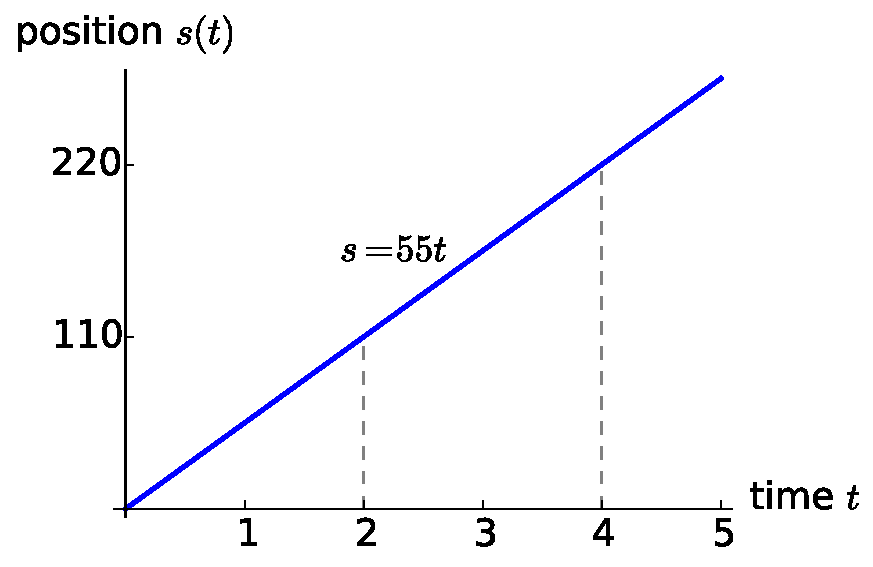
\includegraphics[width=\marginparwidth]{figs/0/linear_position_function.pdf}
\caption{A linear position function.}
\label{fig:0-linear_position_function}
\end{marginfigure}

Also notice that with linear functions, the slope is constant, meaning the slope is the same at every point and over every interval.  So if we wish to know the average or instantaneous rate of change of a linear function, we simply need to calculate the slope of the line!

\begin{marginfigure}[1in] % MARGIN FIGURE
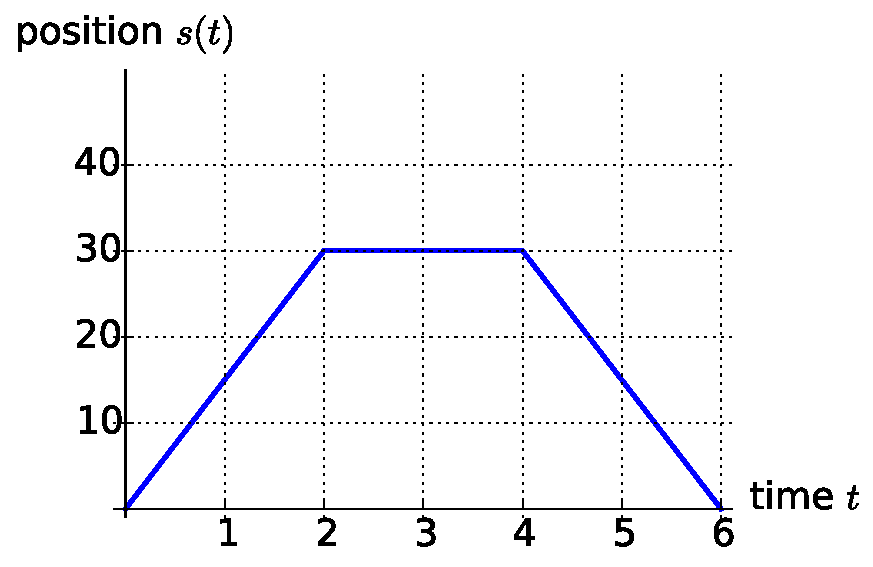
\includegraphics[width=\marginparwidth]{figs/0/piecewise_linear_position_function.pdf}
\caption{A piece-wise linear position function.}
\label{fig:0-piecewise_linear_position_function}
\end{marginfigure}

\begin{example} % EXAMPLE
Use Figure \ref{fig:0-piecewise_linear_position_function} to determine the instantaneous rate of change, or velocity, of the car at $t = 1$, $t = 3$, and $t = 5$. 

\solution When $t = 1$, the position of the car is determined by the line segment passing through the points $(0,0)$ and $(2,3)$.  The slope of that segment is then
\[ \mbox{slope} = \frac{30 - 0}{2 - 0} = \frac{30}{2} = 15, \]
and so the instantaneous rate of change of the car is 15 miles per hour at $t = 1$.

When $t = 3$, the position of the car is determined by the line segment passing through the points $(2,30)$ and $(4,30)$.  The slope of that segment is
\[ \mbox{slope} = \frac{30 - 30}{4 - 2} = 0, \]
and so the instantaneous rate of change of the car is 0 miles per hour at $t = 3$.

Finally, when $t = 5$, the position of the car is determined by the line segment passing through the points $(4,30)$ and $(6,0)$.  The slope of that segment is then
\[ \mbox{slope} = \frac{30 - 0}{4 - 6} = \frac{30}{-2} = -15, \]
and so the instantaneous rate of change of the car is $-15$ miles per hour at $t = 5$.
\end{example}

Now suppose the velocity of the car is constant at $v = 55$ miles per hour starting at time $t=0$. If we wanted to find the position of the car after $t=3$ hours, then we would simply use the equation
\begin{eqnarray*}
\mbox{position}	& = & \mbox{rate} \times \mbox{time} \\
& = & 55 \mbox{ miles per hour} \times 3 \mbox{ hours} \\
& = & 165 \mbox{ miles.} 
\end{eqnarray*}

\begin{marginfigure} % MARGIN FIGURE
\margingraphics{figs/0/constant_velocity_function.pdf}
\caption{The constant velocity function.}
\label{fig:0-constant_velocity_function}
\end{marginfigure}

\begin{marginfigure} % MARGIN FIGURE
\captionsetup[subfigure]{labelformat=empty}
\subfloat{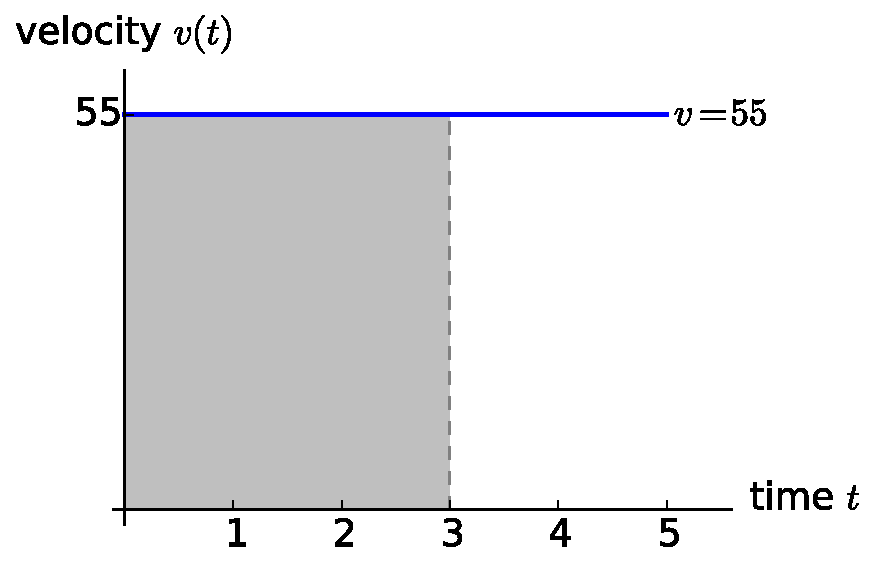
\includegraphics[width=\marginparwidth]{figs/0/position_t3.pdf}}

\subfloat{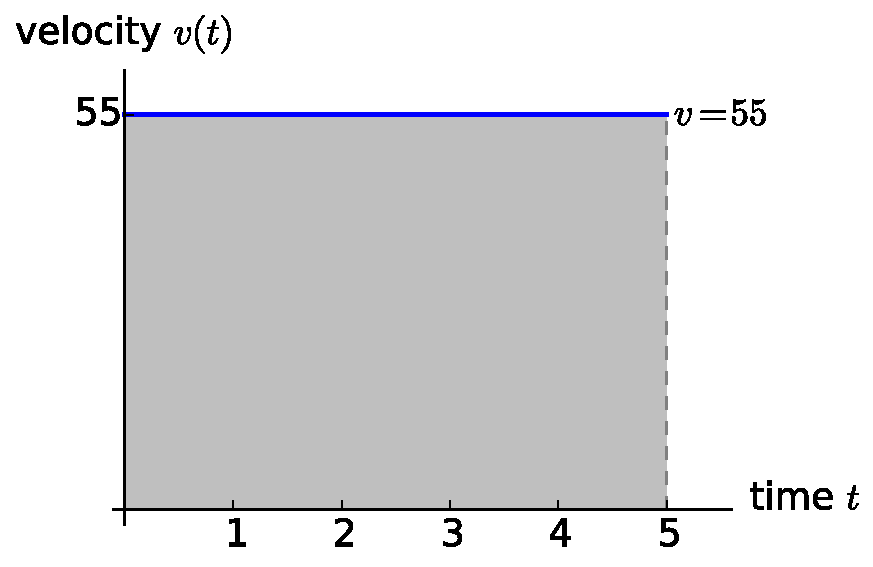
\includegraphics[width=\marginparwidth]{figs/0/position_t5.pdf}}
\caption{Position at $t=3$ and $t=5$ represented by the area of a rectangle.}
\label{fig:0-position_t5}
\end{marginfigure}

\begin{marginfigure}[.5in] % MARGIN FIGURE
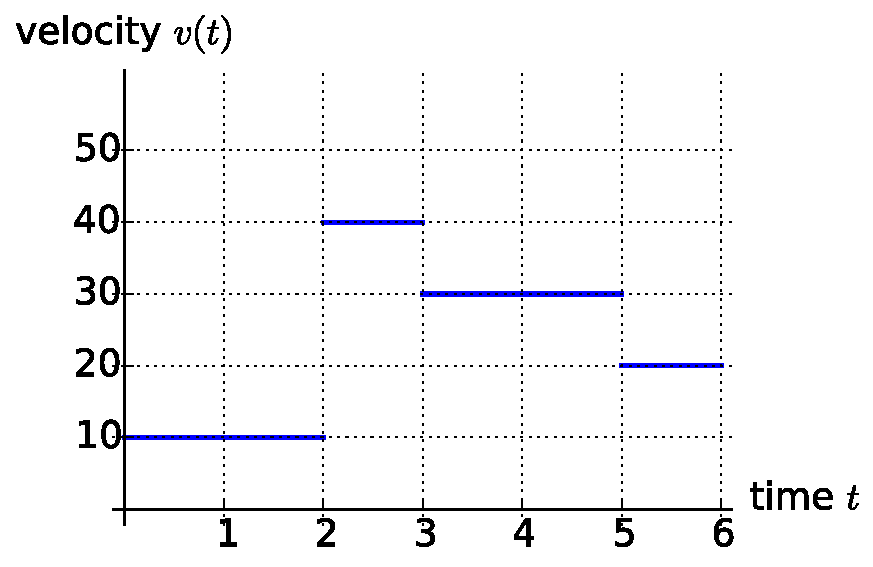
\includegraphics[width=\marginparwidth]{figs/0/piecewise_constant_velocity.pdf}
\caption{A piece-wise constant velocity function.}
\label{fig:0-piecewise_constant_velocity}
\end{marginfigure}

After $5$ hours, the postion would be
\begin{eqnarray*}
\mbox{position}	& = & \mbox{rate} \times \mbox{time} \\
& = & 55 \mbox{ miles per hour} \times 5 \mbox{ hours} \\
& = & 275 \mbox{ miles.} 
\end{eqnarray*}

Geometrically, we can represent the position of the car after 3 hours by the area of the rectangle created by the constant function $v(t) = 55$, the $t$-axis, and the vertical lines $t = 0$ and $t = 3$.  Similarly, we can represent the position after 5 hours geometrically as the area of the region bounded by the $t$-axis and $v(t) = 55$ from $t = 0$ to $t = 5$.  Notice that  region is also a rectangle with height equal to $55$ and width equal to $5 - 0 = 5$.

So in general, if we have a piece-wise constant function--a function consisting of segments of horizontal lines--that represents the velocity of the car (or any other object!), then we can find the position of the car at time $t$ by summing the areas of the rectangles underneath the piece-wise constant function from time $0$ to time $t$.

\begin{example} % EXAMPLE
Use Figure \ref{fig:0-piecewise_constant_velocity} to determine the position of the car at time $t=6$.

\solution In the figure, there are four horizontal line segments that comprise the piece-wise constant function.  So there will be four rectangles whose areas we must calculate, and then we will sum those areas to determine the position of the car at $t=6$.

From $t = 0$ to $t = 2$, the rectangle has height $10$ and width $2$; therefore, its area is $10 \times 2 = 20$.

From $t = 2$ to $t = 3$, the rectangle has height $40$ and width $1$; therefore, its area is $40 \times 1 = 40$.

From $t = 3$ to $t = 5$, the rectangle has height $30$ and width $2$; therefore, its area is $30 \times 2 = 60$.

And from $t = 5$ to $t = 6$, the rectangle has height $20$ and width $1$; therefore, its area is $20 \times 1 = 20$.

So the position of the car at $t = 6$ is $20 + 40 + 60 + 20 = 140$ miles.
\end{example}

What if the velocity function is a piece-wise linear function instead of a piece-wise constant function as seen in Figure~\ref{fig:0-piecewise_linear_velocity}?  Nothing changes with respect to {\em how} we find the position--we still must find the area underneath the function, but the region(s) may not be rectangular.  They may be triangles, trapezoids, or rectangles, which means we may need to remember the area formulas for those polygons.  But it is certainly possible to calculate the position from a piece-wise linear velocity function using only algebra.

\begin{marginfigure} % MARGIN FIGURE
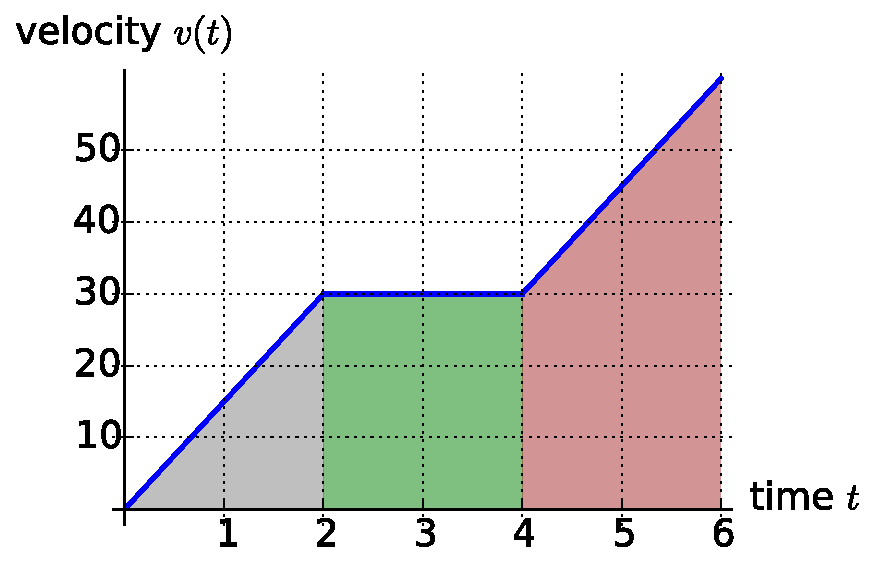
\includegraphics[width=\marginparwidth]{figs/0/piecewise_linear_velocity.pdf}
\caption{A piece-wise linear velocity function.}
\label{fig:0-piecewise_linear_velocity}
\end{marginfigure}

\concept{Slope and Area}{ % CONCEPT
The slope of the position graph $s$ at some point gives the velocity $v$ at that point. The area of the region underneath the velocity graph $v$ from time $0$ to time $t$ gives the position $s$ at time $t$.
}% end concept

So what if we wish to find the instantaneous rate of change, or slope, of a function that is not piece-wise linear?  Or what if we wish to find the total accumulated amount of some quantity, or the area of a region underneath a function, when that function is not piece-wise linear?  Continue reading...

\cleardoublepage
\section{How do we measure velocity?} \label{S:0.2.Velocity}

\begin{goals}
\item How is the average velocity of a moving object connected to the values of its position function?
\item How do we interpret the average velocity of an object geometrically with regard to the graph of its position function?
\item How is the notion of instantaneous velocity connected to average velocity?
\end{goals}

%--------------------------------------
% SUBSECTION INTRODUCTION
%--------------------------------------

\subsection*{Introduction}

We begin with a familiar problem:  a ball being tossed straight up in the air from an initial height.  From this elementary scenario, we will ask questions about how the ball is moving.  These questions will lead us to begin investigating ideas that will be central throughout our study of differential calculus and that have wide-ranging consequences.  In a great deal of our thinking about calculus, we will be well-served by remembering this first example and asking ourselves how the various (sometimes abstract) ideas we are considering are related to the simple act of tossing a ball straight up in the air.  

\begin{pa} \label{PA:0.2}
Suppose that the height $s$ of a ball (in feet) at time $t$ (in seconds) is given by the formula $s(t) = 64 - 16(t-1)^2$.  
\ba
\item Construct an accurate graph of $y = s(t)$ on the time interval $0 \le t \le 3$.  Label at least six distinct points on the graph, including the three points that correspond to when the ball was released, when the ball reaches its highest point, and when the ball lands.

\item In everyday language, describe the behavior of the ball on the time interval $0 < t < 1$ and on time interval $1 < t < 3$.  What occurs at the instant $t = 1$?

\item Consider the expression 
\[ AV_{[0.5,1]} = \frac{s(1) - s(0.5)}{1-0.5}. \]
Compute the value of $AV_{[0.5,1]}$.  What does this value measure geometrically?  What does this value measure physically?  In particular, what are the units on $AV_{[0.5,1]}$?
\ea
\end{pa} \afterpa %Preview ACTIVITY 

%-----------------------------------------------------------------
% SUBSECTION POSITION AND AVERAGE VELOCITY
%-----------------------------------------------------------------
\subsection*{Position and average velocity}

Any moving object has a \emph{position}\index{position} that can be considered a function of \emph{time}.  When this motion is along a straight line, the position is given by a single variable, and we usually let this position be denoted by $s(t)$, which reflects the fact that position is a function of time.  For example, we might view $s(t)$ as telling the mile marker of a car traveling on a straight highway at time $t$ in hours; similarly, the function $s$ described in Preview Activity \ref{PA:0.2} is a position function, where position is measured vertically relative to the ground.

Not only does such a moving object have a position associated with its motion, but on any time interval, the object has an \emph{average velocity}\index{average velocity}.   Think, for example, about driving from one location to another:  the vehicle travels some number of miles over a certain time interval (measured in hours), from which we can compute the vehicle's average velocity.  In this situation, average velocity is the number of miles traveled divided by the time elapsed, which of course is given in \emph{miles per hour}. Similarly, the calculation of $A_{[0.5,1]}$ in Preview Activity \ref{PA:0.2} found the average velocity of the ball on the time interval $[0.5,1]$, measured in feet per second.

In general, we make the following definition:  for an object moving in a straight line whose position at time $t$ is given by the function $s(t)$, the \emph{average velocity\index{average velocity} of the object on the interval from $t = a$ to $t = b$}, denoted $AV_{[a,b]}$, is given by the formula
\[ AV_{[a,b]} = \frac{s(b)-s(a)}{b-a}. \]
Note well: the units on $AV_{[a,b]}$ are 
``units of $s$ per unit of $t$,'' such as ``miles per hour'' or ``feet per second.''

\begin{marginfigure}[6cm] % MARGIN FIGURE
\margingraphics{figs/0/0-2_Act1.pdf}
\caption{A partial plot of $s(t) = 64 - 16(t-1)^2$.} \label{fig:0.2.Act1}
\end{marginfigure}

\begin{activity} \label{A:0.2.1}  The following questions concern the position function given by $s(t) = 64 - 16(t-1)^2$, which is the same function considered in Preview Activity \ref{PA:0.2}.
\ba
	\item Compute the average velocity of the ball on each of the following time intervals: $[0.4,0.8]$, $[0.7,0.8]$, $[0.79, 0.8]$, $[0.799,0.8]$, $[0.8,1.2]$, $[0.8,0.9]$, $[0.8,0.81]$, $[0.8,0.801]$.  Include units for each value.
	\item On the provided graph in Figure~\ref{fig:0.2.Act1}, sketch the line that passes through the points $A=(0.4, s(0.4))$ and $B=(0.8, s(0.8))$.  What is the meaning of the slope of this line?  In light of this meaning, what is a geometric way to interpret each of the values computed in the preceding question?
	\item Use a graphing utility to plot the graph of $s(t) = 64 - 16(t-1)^2$ on an interval containing the value $t = 0.8$.  Then, zoom in repeatedly on the point $(0.8, s(0.8))$.  What do you observe about how the graph appears as you view it more and more closely?  
	\item What do you conjecture is the velocity of the ball at the instant $t = 0.8$?  Why?
\ea
\end{activity}
\begin{smallhint}
\ba
	\item On $[0.4,0.8]$, the average velocity is $AV_{[0.4,0.8]} = \frac{s(0.8)-s(0.4)}{0.8-0.4}$ ft/sec.
	\item Remember that the slope of a line can be found by taking ``rise over run.''  In this context, the slope is found by computing ``change in $s$ over change in $t$.''
	\item While the curve $s(t)$ is a parabola, how does it look up close on a very small interval? 
	\item ``Instantaneous'' velocity can be approximated by average velocity on a very small interval.
\ea
\end{smallhint}
\begin{bighint}
\ba
	\item On $[0.4,0.8]$, the average velocity is $AV_{[0.4,0.8]} = \frac{s(0.8)-s(0.4)}{0.8-0.4}$ ft/sec.  Each of the other average velocities is computed similarly.
	\item Remember that the slope of a line can be found by taking ``rise over run.''  In this context, the slope is found by computing ``change in $s$ over change in $t$.''  Note that each average velocity $\frac{s(b)-s(a)}{b-a}$ can be viewed as the slope of a line between $(a,s(a))$ and $(b,s(b))$.
	\item While the curve $s(t)$ is a parabola, how does it look up close on a very small interval?  What type of familiar function seems to emerge?
	\item ``Instantaneous'' velocity can be approximated by average velocity on a very small interval.  Are the numbers you computed in (a) getting close to a particular value as we look at smaller and smaller intervals surrounding $t = 0.8$?
\ea
\end{bighint}
\begin{activitySolution}
\ba
	\item On $[0.4,0.8]$, the average velocity is $AV_{[0.4,0.8]} = \frac{s(0.8)-s(0.4)}{0.8-0.4} = \frac{63.36-58.24}{0.4} = 12.8$ ft/sec.  On $[0.7,0.8]$, the average velocity is 8 ft/sec.  The other average velocities are, respectively (in the order of the intervals listed in the activity), 6.56, 6.416, 0, 4.8, 6.24, 6.384, all measured in feet per second.
	\item The slope of the line between $A(0.4, s(0.4))$ and $B(0.8, s(0.8))$ is $\frac{s(0.8)-s(0.4)}{0.8-0.4} = 12.8$.  This is precisely the average velocity of the ball between $t = 0.4$ and $t = 0.8$, and indeed each of the average velocities computed in (a) can be viewed as the slope of the line joining the points $(a,s(a))$ and $(b,s(b))$.
	\begin{center}
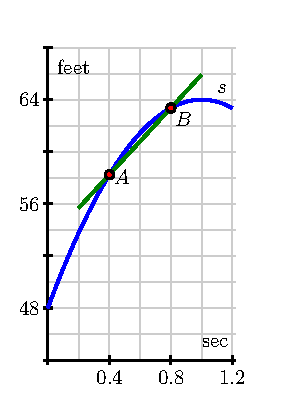
\includegraphics{figures/1_1_Act1Soln.eps}
\end{center}
	\item As we zoom in on the curve $s(t) = 64 - 16(t-1)^2$ at the point $(0.5, 60)$, the graph begins to look like a straight line.  Indeed, it appears to look like a straight line with slope about 6.4.
	\item Observe that the average velocity of the ball on the intervals $[0.799,0.8]$ and $[0.8,0.801]$ is 6.416 and 6.384 feet/sec respectively.  Hence it appears that the ball's velocity at the instant $t = 0.8$ should be about 6.4 feet per second.
\ea
\end{activitySolution}
\aftera %ACTIVITY 

%-----------------------------------------------------
% SUBSECTION INSTANTANEOUS VELOCITY
%-----------------------------------------------------
\subsection*{Instantaneous Velocity}

Whether driving a car, riding a bike, or throwing a ball, we have an intuitive sense that any moving object has a velocity at any given moment -- a number that measures how fast the object is moving \emph{right now}.  For instance, a car's speedometer tells the driver what appears to be the car's velocity at any given instant.  In fact, the posted velocity on a speedometer is really an average velocity that is computed over a very small time interval (by computing how many revolutions the tires have undergone to compute distance traveled), since velocity fundamentally comes from considering a change in position divided by a change in time.  But if we let the time interval over which average velocity is computed become shorter and shorter, then we can progress from average velocity to \emph{instantaneous} velocity.  

Informally, we define the \emph{instantaneous velocity}\index{instantaneous velocity} of a moving object at time $t = a$ to be the value that the average velocity approaches as we take smaller and smaller intervals of time containing $t = a$ to compute the average velocity.  We will develop a more formal definition of this momentarily, one that will end up being the foundation of much of our work in first semester calculus.  For now, it is fine to think of instantaneous velocity this way:  take average velocities on smaller and smaller time intervals, and if those average velocities approach a single number, then that number will be the instantaneous velocity at that point.

\begin{activity}  \label{A:0.2.2}
Each of the following questions concern  $s(t) = 64 - 16(t-1)^2$, the position function from Preview Activity \ref{PA:0.2}.
\ba
	\item Compute the average velocity of the ball on the time interval $[1.5,2]$.  What is different between this value and the average velocity on the interval $[0,0.5]$?
	\item Use appropriate computing technology to estimate the instantaneous velocity of the ball at $t = 1.5$.  Likewise, estimate the instantaneous velocity of the ball at $t = 2$.  Which value is greater?
	\item How is the sign of the instantaneous velocity of the ball related to its behavior at a given point in time?  That is, what does positive instantaneous velocity tell you the ball is doing?  Negative instantaneous velocity?
	\item Without doing any computations, what do you expect to be the instantaneous velocity of the ball at $t = 1$?  Why?
\ea
\end{activity}
\begin{smallhint}
\ba
	\item Remember to use the formula for average velocity from above:  $AV_{[a,b]} = \frac{s(b)-s(a)}{b-a}$.  Think carefully about whether certain quantities are positive or negative.
	\item To estimate the instantaneous velocity at $t = 1.5$, consider average velocities on the intervals $[1.499,1.5]$ and $[1.5,1.501]$.
	\item Think about whether the ball is rising or falling.
	\item What is the average velocity of the ball on small intervals that contain $t = 0$?
\ea
\end{smallhint}
\begin{bighint}
\ba
	\item $AV_{[1.5,2]} = \frac{s(2)-s(1.5)}{2-1.5}$.  Your result should be negative since $s(2) < s(1.5)$.
	\item To estimate the instantaneous velocity at $t = 1.5$, consider average velocities on the intervals $[1.499,1.5]$ and $[1.5,1.501]$.
	\item You should find in (a) that the instantaneous velocity at $t = 1.5$ is negative, while earlier we found that the instantaneous velocity at $t = 0.5$ is positive.  How are these signs connected to whether the ball is rising or falling?
	\item Think about the line through the points $(0.999,s(0.999))$ and $(1,s(1))$ will look like given the ``special'' role of $(1,s(1))$ on the graph of $s(t)$.
\ea
\end{bighint}
\begin{activitySolution}
\ba
	\item $AV_{[1.5,2]} = \frac{s(2)-s(1.5)}{2-1.5} = -24$ ft/sec.  We note that this average velocity is negative, and in fact is the opposite of the average velocity of 24 ft/sec on the interval $[0,0.5]$.
	\item Since $AV_{[1.499,1.5]} = -15.984$ and $AV_{[1.5, 1.501]} = -16.016$, it appears that the instantaneous velocity of the ball at $t = 1.5$ is approximately $-16$ ft/sec.  Similar computations show that at $t = 2$, it appears the instantaneous velocity is about $-32$ ft/sec.  Note that $-16>-32$, so the instantaneous velocity at $t = 1.5$ is greater because it is ``less negative.'' Asking which number is ``greater'' is different from asking which number is ``more negative.''
	\item When the ball is rising, its instantaneous velocity is positive, while when the ball is falling, its instantaneous velocity is negative.
	\item Note that $(1,s(1))$ is the vertex of the parabola given by $s(t)$.  At this point, the ball is neither rising nor falling.  On intervals of the form $[a,1]$, where $a < 1$, the average velocity of the ball is positive; on intervals of form $[1,b]$, where $b > 1$, the average velocity is positive.  Hence we expect the instantaneous velocity of the ball at the moment $t = 1$ to be zero.
\ea
\end{activitySolution}
\aftera
 %ACTIVITY 

At this point we have started to see a close connection between average velocity and instantaneous velocity, as well as how each is connected not only to the physical behavior of the moving object but also to the geometric behavior of the graph of the position function.  In order to make the link between average and instantaneous velocity more formal, we will introduce the notion of \emph{limit} in Section~\ref{S:1.1.Limits}.  As a preview of that concept, we look at a way to consider the limiting value of average velocity through the introduction of a parameter.  Note that if we desire to know the instantaneous velocity at $t = a$ of a moving object with position function $s$, we are interested in computing average velocities on the interval $[a,b]$ for smaller and smaller intervals.  One way to visualize this is to think of the value $b$ as being $b = a + h$, where $h$ is a small number that is allowed to vary.  Thus, we observe that the average velocity of the object on the interval $[a,a+h]$ is
\[ AV_{[a,a+h]} = \frac{s(a+h)-s(a)}{h}, \]
with the denominator being simply $h$ because $(a+h) - a = h$.  Initially, it is fine to think of $h$ being a small positive real number; but it is important to note that we allow $h$ to be a small negative number, too, as this enables us to investigate the average velocity of the moving object on intervals prior to $t = a$, as well as following $t = a$.  When $h < 0$, $AV_{[a,a+h]}$ measures the average velocity on the interval $[a+h,a]$.  

To attempt to find the instantaneous velocity at $t = a$, we investigate what happens as the value of $h$ approaches zero.  We consider this further in the following example.

\begin{example}
For a falling ball whose position function is given by \newline $s(t) = 16 - 16t^2$ where $s$ is measured in feet and $t$ in seconds, find an expression for the average velocity of the ball on a time interval of the form $[0.5, 0.5+h]$ where $-0.5 < h < 0.5$ and $h \ne 0$.  Use this expression to compute the average velocity on $[0.5,0.75]$ and $[0.4,0.5]$, as well as to make a conjecture about the instantaneous velocity at $t = 0.5$.

\solution We make the assumptions that $-0.5 < h < 0.5$ and $h \ne 0$ because $h$ cannot be zero (otherwise there is no interval on which to compute average velocity) and because the function only makes sense on the time interval $0 \le t \le 1$, as this is the duration of time during which the ball is falling.  Observe that we want to compute and simplify $$AV_{[0.5, 0.5+h]} = \frac{s(0.5+h) - s(0.5)}{(0.5+h) - 0.5}.$$  The most unusual part of this computation is finding $s(0.5+h)$.  To do so, we follow the rule that defines the function $s$.  In particular, since $s(t) = 16-16t^2$, we see that 
\begin{eqnarray*}
s(0.5+h) & = & 16 - 16(0.5 + h)^2 \\
& = & 16 - 16(0.25 + h + h^2) \\
& = & 16 - 4 - 16h - 16h^2 \\
& = & 12 - 16h - 16h^2.
\end{eqnarray*}
Now, returning to our computation of the average velocity, we find that 
\begin{eqnarray*}
 AV_{[0.5, 0.5+h]} & = & \frac{s(0.5+h) - s(0.5)}{(0.5+h) - 0.5} \\
& = & \frac{(12 - 16h - 16h^2) - (16 - 16(0.5)^2)}{0.5 + h - 0.5} \\
& = & \frac{12 - 16h - 16h^2 - 12}{h} \\
& = & \frac{-16h - 16h^2}{h}.
\end{eqnarray*}
At this point, we note two things:  first, the expression for average velocity clearly depends on $h$, which it must, since as $h$ changes the average velocity will change.  Further, we note that since $h$ can never equal zero, we may further simplify the most recent expression.  Removing the common factor of $h$ from the numerator and denominator, it follows that
$$ AV_{[0.5, 0.5+h]} = -16 - 16h.$$
Now, for any small positive or negative value of $h$, we can compute the average velocity.  For instance, to obtain the average velocity on $[0.5,0.75]$, we let $h = 0.25$, and the average velocity is $-16 - 16(0.25) = -20$ ft/sec.  To get the average velocity on $[0.4, 0.5]$, we let $h = -0.1$, which tells us the average velocity is $-16 - 16(-0.1) = -14.4$ ft/sec.  Moreover, we can even explore what happens to $AV_{[0.5, 0.5+h]}$ as $h$ gets closer and closer to zero.  As $h$ approaches zero, $-16h$ will also approach zero, and thus it appears that the instantaneous velocity of the ball at $t = 0.5$ should be $-16$ ft/sec.
\end{example} % EXAMPLE

\begin{activity} \label{A:1.1.3}
For the function given by $s(t) = 64 - 16(t-1)^2$ from Preview Activity \ref{PA:0.2}, find the most simplified expression you can for the average velocity of the ball on the interval $[2, 2+h]$.  Use your result to compute the average velocity on $[1.5,2]$ and to estimate the instantaneous velocity at $t = 2$.  Finally, compare your earlier work in Activity~\ref{A:0.2.1}.
\end{activity} 
\begin{smallhint}
Note that $s(2+h) = 64 - 16(2+h-1)^2 = 64 - 16(1+h)^2 = 64 - (16 + 32h + 16h^2) = 48 - 32h - 16h^2$.
\end{smallhint}
\begin{bighint}
Note that $s(2+h) = 64 - 16(2+h-1)^2 = 64 - 16(1+h)^2 = 64 - (16 + 32h + 16h^2) = 48 - 32h - 16h^2$, and then recall that $AV_{[2, 2+h]} = \frac{s(2+h) - s(2)}{h}$.  Finally, you can use a negative value for $h$ to help you find the desired average velocity.
\end{bighint}
\begin{activitySolution}
Observe first that $s(2+h) = 64 - 16(2+h-1)^2 = 64 - 16(1+h)^2 = 64 - (16 + 32h + 16h^2) = 48 - 32h - 16h^2$.  Next, recall that $AV_{[2, 2+h]} = \frac{s(2+h) - s(2)}{h}$, so
$$AV_{[2, 2+h]} = \frac{s(2+h) - s(2)}{h} = \frac{(48 - 32h - 16h^2)-48}{h} = \frac{-32h - 16h^2}{h}.$$
Now, since we assume $h \ne 0$, we can simplify further to find that $AV_{[2, 2+h]} = -32 - 16h$.  Setting $h = -0.5$, it follows $AV_{[1.5,2]} = -32 + 16(0.5) = -24$ ft/sec, and letting $h$ approach zero, we see that $-32 - 16h$ will approach $-32$, so the instantaneous velocity at $t = 2$ appears to be $-32$ feet/sec.  Both results match our earlier work in Activity~\ref{A:0.2.1}.
\end{activitySolution}
\aftera % ACTIVITY

\clearpage

%--------------
% SUMMARY
%--------------
%\begin{marginfigure}[-3.5in] % MARGIN FIGURE
%\margingraphics{figs/0/0-2_Summary.pdf} 
%\caption{The graph of position function $s$ together with the line through $(a,s(a))$ and $(b,s(b))$ whose slope is $m = \frac{s(b)-s(a)}{b-a}$.  The line's slope is the average rate of change of $s$ on the interval $[a,b]$.} \label{F:0.2.Summary}
%\end{marginfigure}
\vspace*{-1cm}
\begin{summary}
\item The average velocity on $[a,b]$ can be viewed geometrically as the slope of the line between the points $(a,s(a))$ and $(b,s(b))$ on the graph of $y = s(t)$, as shown below.% in Figure~\ref{F:0.2.Summary}.

\begin{center}
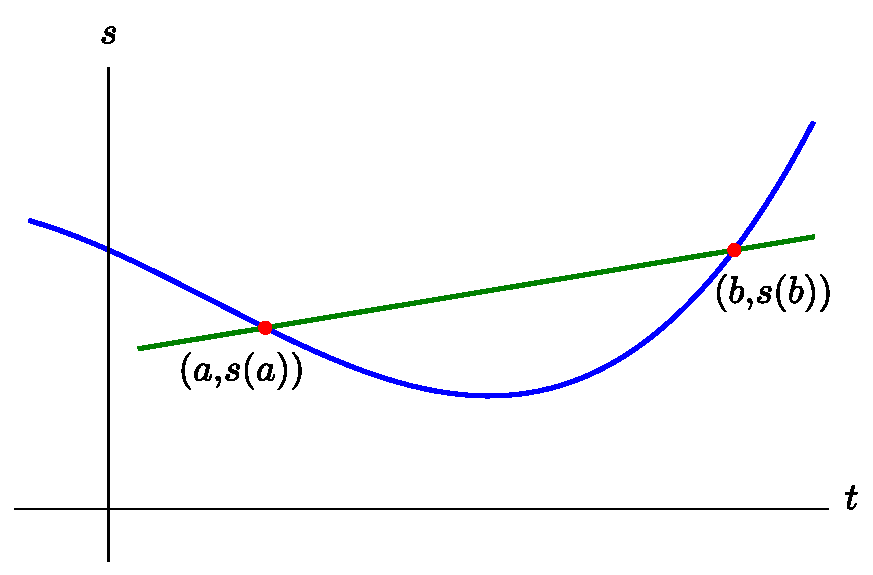
\includegraphics[scale=.35]{figs/0/0-2_Summary.pdf}
\end{center}

\item Given a moving object whose position at time $t$ is given by a function $s$, the average velocity of the object on the time interval $[a,b]$ is given by $AV_{[a,b]} = \frac{s(b) - s(a)}{b-a}$.  Viewing the interval $[a,b]$ as having the form $[a,a+h]$, we equivalently compute average velocity by the formula $AV_{[a,a+h]} = \frac{s(a+h) - s(a)}{h}$.

\item The instantaneous velocity of a moving object at a fixed time is estimated by considering average velocities on shorter and shorter time intervals that contain the instant of interest.
\end{summary}

\clearpage

%-------------------------------
% SUBSECTION EXERCISES
%-------------------------------
\begin{exercises} 

\item \label{Ez:1.1.1} A bungee jumper dives from a tower at time $t=0$.   Her height $h$ (measured in feet) at time $t$ (in seconds) is given by the graph in Figure~\ref{F:1.1.Ez1}.

\begin{marginfigure}[.5cm]
\margingraphics{figures/1_1_Ez1.eps}
\caption{A bungee jumper's height function.} \label{F:1.1.Ez1}
\end{marginfigure}

In this problem, you may base your answers on estimates from the graph or use the fact that the jumper's height function is given by $s(t) = 100\cos(0.75t) \cdot e^{-0.2t}+100$.
  \ba
	\item What is the change in vertical position of the bungee jumper between $t=0$ and $t=15$?
	\item Estimate the jumper's average velocity on each of the following time intervals:  $[0,15]$, $[0,2]$, $[1,6]$, and $[8,10]$.  Include units on your answers.
	\item On what time interval(s) do you think the bungee jumper achieves her greatest average velocity?  Why? 
	\item Estimate the jumper's instantaneous velocity at $t=5$.  Show your work and explain your reasoning, and include units on your answer.
	\item Among the average and instantaneous velocities you computed in earlier questions, which are positive and which are negative?  What does negative velocity indicate?
  \ea 

\begin{exerciseSolution}
\end{exerciseSolution}
\item A diver leaps from a $3$ meter springboard.  His feet leave the board at time $t=0$, he reaches his maximum height of $4.5$ m at $t = 1.1$ seconds, and enters the water at $t = 2.45$.  Once in the water, the diver coasts to the bottom of the pool (depth $3.5$ m), touches bottom at $t=7$, rests for one second, and then pushes off the bottom.  From there he coasts to the surface, and takes his first breath at $t=13$.

\ba
  \item Let $s(t)$ denote the function that gives the height of the diver's feet (in meters) above the water at time $t$.  (Note that the ``height'' of the bottom of the pool is $-3.5$ meters.)  Sketch a carefully labeled graph of $s(t)$ on the provided axes in Figure~\ref{F:1.1.Ez2}.  Include scale and units on the vertical axis.  Be as detailed as possible.

\begin{figure}[h]
  \begin{center}
 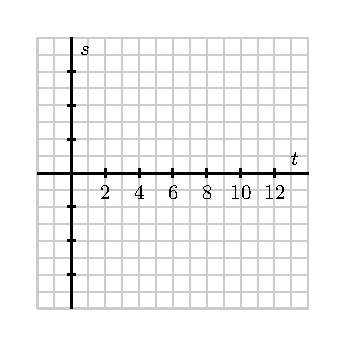
\includegraphics{figures/1_1_Ez2a.eps} \ \  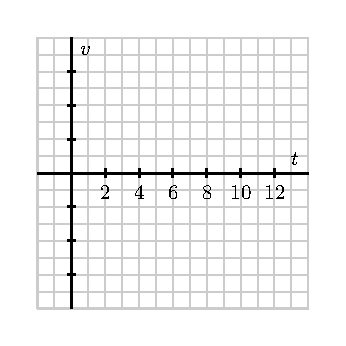
\includegraphics{figures/1_1_Ez2b.eps}
   \end{center}
   \caption{Axes for plotting $s(t)$ in part (a) and $v(t)$ in part (c) of the diver problem.} \label{F:1.1.Ez2}
\end{figure}

  \item Based on your graph in (a), what is the average velocity of the diver between $t = 2.45$ and $t=7$?  Is his average velocity the same on every time interval within $[2.45,7]$? 

  \item Let the function $v(t)$ represent the \emph{instantaneous vertical velocity} of the diver at time $t$ (i.e.~the speed at which the height function $s(t)$ is changing; note that velocity in the upward direction is positive, while the velocity of a falling object is negative).  Based on your understanding of the diver's behavior, as well as your graph of the position function, sketch a carefully labeled graph of $v(t)$ on the axes provided  in Figure~\ref{F:1.1.Ez2}.  Include scale and units on the vertical axis.  Write several sentences that explain how you constructed your graph, discussing when you expect $v(t)$ to be zero, positive, negative, relatively large, and relatively small.
  \item Is there a connection between the two graphs that you can describe?  What can you say about the velocity graph when the height function is increasing?  decreasing?  Make as many observations as you can.
\ea
\begin{exerciseSolution}
\end{exerciseSolution}

\item According to the U.S. census, the population of the city of Grand Rapids, MI, was $181,843$ in $1980$; $189,126$ in $1990$; and $197,800$ in $2000$.

\ba
	\item Between $1980$ and $2000$, by how many people did the population of Grand Rapids grow?
	\item In an average year between $1980$ and $2000$, by how many people did the population of Grand Rapids grow?
	\item Just like we can find the average velocity of a moving body by computing change in position over change in time, we can compute the average rate of change of any function $f$.  In particular, the \emph{average rate of change} of a function $f$ over an interval $[a,b]$ is the quotient
$$\frac{f(b)-f(a)}{b-a}.$$  
What does the quantity $\frac{f(b)-f(a)}{b-a}$ measure on the graph of $y = f(x)$ over the interval $[a,b]$?
	\item Let $P(t)$ represent the population of Grand Rapids at time $t$, where $t$ is measured in years from January $1$, $1980$.  What is the average rate of change of $P$ on the interval $t = 0$ to $t = 20$?  What are the units on this quantity?
	\item If we assume the the population of Grand Rapids is growing at a rate of approximately $4$\% per decade,  we can model the population function with the formula $$P(t) = 181843 (1.04)^{t/10}.$$  Use this formula to compute the average rate of change of the population on the intervals $[5,10]$, $[5,9]$, $[5,8]$, $[5,7]$, and $[5,6]$.
	\item How fast do you think the population of Grand Rapids was changing on January $1$, $1985$?  Said differently, at what rate do you think people were being added to the population of Grand Rapids as of January $1$, $1985$?  How many additional people should the city have expected in the following year?  Why?
\ea

\end{exercises}
\afterexercises
 

\cleardoublepage
\chapter{Limits}\label{CH:1}

\section{The notion of limit} \label{S:1.1.Limits}

\begin{goals}
\item What is the behavior of a function arbitrarily close to, but not necessarily at, a specific point?
\item What is the mathematical notion of \emph{limit} and what role do limits play in the study of functions?
\item What is the meaning of the notation $\ds \lim_{x \to a} f(x) = L$?
\item How do we go about determining the value of the limit of a function at a point?
\item How does the notion of limit allow us to move from average velocity to instantaneous velocity?
\end{goals}

%-----------------------------------
% SUBSECTION INTRODUCTION
%-----------------------------------
\subsection*{Introduction}

Functions are at the heart of mathematics: a function is a process or rule that associates each individual input to exactly one corresponding output.  Students learn in courses prior to calculus that there are many different ways to represent functions, including through formulas, graphs, tables, and even words.  For example, the squaring function can be thought of in any of these ways.  In words, the squaring function takes any real number $x$ and computes its square.  The formulaic and graphical representations go hand in hand, as $y = f(x) = x^2$ is one of the simplest curves to graph.  Finally, we can also partially represent this function through a table of values, essentially by listing some of the ordered pairs that lie on the curve, such as  $(-2,4)$, $(-1,1)$, $(0,0)$, $(1,1)$, and $(2,4)$.

Functions are especially important in calculus because they often model important phenomena -- the location of a moving object at a given time, the rate at which an automobile is consuming gasoline at a certain velocity, the reaction of a patient to the size of a dose of a drug -- and calculus can be used to study how these output quantities change in response to changes in the input variable.  Moreover, thinking about concepts like average and instantaneous velocity leads us naturally from an initial function to a related, sometimes more complicated function.  As one example of this, think about the falling ball whose position function is given by $s(t) = 64 - 16t^2$ and the average velocity of the ball on the interval $[1,x]$.  Observe that
\[ AV_{[1,x]} = \frac{s(x) - s(1)}{x-1} = \frac{(64-16x^2) - (64-16)}{x-1} = \frac{16 - 16x^2}{x-1}. \]
Now, two things are essential to note:  this average velocity depends on $x$ (indeed, $AV_{[1,x]}$ is a function of $x$), and our most focused interest in this function occurs near $x = 1$, which is where the function is not defined.  Said differently, the function $g(x) = \frac{16 - 16x^2}{x-1}$ tells us the average velocity of the ball on the interval from $t = 1$ to $t = x$, and if we are interested in the instantaneous velocity of the ball when $t = 1$, we'd like to know what happens to $g(x)$ as $x$ gets closer and closer to $1$.  At the same time, $g(1)$ is not defined, because it leads to the quotient $0/0$.

This is where the idea of \emph{limits} comes in.  By using a limit, we'll be able to allow $x$ to get arbitrarily close, but not equal, to $1$ and fully understand the behavior of $g(x)$ near this value.  We'll develop key language, notation, and conceptual understanding in what follows, but for now we consider a preliminary activity that uses the graphical interpretation of a function to explore points on a graph where interesting behavior occurs.

\begin{marginfigure}[8cm]
\margingraphics{figures/1_2_PA1.eps} 
\caption{Graph of $y = g(x)$ for Preview Activity~\ref{PA:1.1}.} \label{fig:1.1.PA1}
\end{marginfigure}

\begin{pa} \label{PA:1.1}
Suppose that $g$ is the function given by the Figure~\ref{fig:1.1.PA1}.  Use the graph to answer each of the following questions. 
\ba
	\item Determine the values $g(-2)$, $g(-1)$, $g(0)$, $g(1)$, and $g(2)$, if defined.  If the function value is not defined, explain what feature of the graph tells you this.
	\item For each of the values $a = -1$, $a = 0$, and $a = 2$, complete the following sentence: ``As $x$ gets closer and closer (but not equal) to $a$, $g(x)$ gets as close as we want to \underline{\hspace{0.3in}}.''
	\item What happens as $x$ gets closer and closer (but not equal) to $a = 1$?  Does the function $g(x)$ get as close as we would like to a single value?
\ea

\end{pa} \afterpa %ACTIVITY

%-----------------------------------------------------------------
% SUBSECTION THE AVERAGE VALUE OF A FUNCTION
%-----------------------------------------------------------------
\subsection*{The Idea of a Limit}

Limits can be thought of as a way to study the tendency or trend of a function as the input variable approaches a fixed value, or even as the input variable increases or decreases without bound.  Here, we focus on what it means to say that ``a function $f$ has limit $L$ as $x$ approaches $a$.''  To begin, we think about a recent example.

In Preview Activity \ref{PA:1.1}, you saw that for the given function $g$, as $x$ gets closer and closer (but not equal) to $0$, $g(x)$ gets as close as we want to the value $4$.  At first, this may feel counterintuitive, because the value of $g(0)$ is $1$, not $4$.  By their very definition, limits regard the behavior of a function \emph{arbitrarily close to} a fixed input, but the value of the function \emph{at} the fixed input does not matter.  More formally\footnote{What follows here is not what mathematicians consider the formal definition of a limit.  To be completely precise, it is necessary to quantify both what it means to say ``as close to $L$ as we like'' and ``sufficiently close to $a$.''  That can be accomplished through what is traditionally called the epsilon-delta definition of limits, which will be covered in Section \ref{S:1.4.precise}.}, we say the following.

\definition{The Limit of a Function}{ %DEFINITION
Given a function $f$, a fixed input $x = a$, and a real number $L$, we say that \emph{$f$ has limit\index{limit!definition} $L$ as $x$ approaches $a$}, and write
\[ \lim_{x \to a} f(x) = L \]
provided that we can make $f(x)$ as close to $L$ as we like by taking $x$ sufficiently close (but not equal) to $a$.  If we cannot make $f(x)$ as close to a single value as we would like as $x$ approaches $a$, then we say that \emph{$f$ does not have a limit as $x$ approaches $a$.}
} % end definition

For the function $g$ pictured in Figure \ref{fig:1.1.PA1}, we can make the following observations:  
\[ \ds \lim_{x \to -1} g(x) = 3, \ \ds \lim_{x \to 0} g(x) = 4, \ \mbox{and} \ \ds \lim_{x \to 2} g(x) = 1, \] 
but $g$ does not have a limit as $x \to 1$.  When working graphically, it suffices to ask if the function approaches a single value from each side of the fixed input, while understanding that the function value right at the fixed input is irrelevant.  This reasoning explains the values of the first three stated limits.  In a situation such as the jump in the graph of $g$ at $x = 1$, the issue is that if we approach $x = 1$ from the left, the function values tend to get as close to $3$ as we'd like, but if we approach $x = 1$ from the right, the function values get as close to $2$ as we'd like, and there is no single number that all of these function values approach.  This is why the limit of $g$ does not exist at $x = 1$.

For any function $f$, there are typically three ways to answer the question ``does $f$ have a limit at $x = a$, and if so, what is the limit?''  The first is to reason graphically as we have just done with the example from Preview Activity \ref{PA:1.1}.  If we have a formula for $f(x)$, there are two additional possibilities:  (1) evaluate the function at a sequence of inputs that approach $a$ on either side, typically using some sort of computing technology, and ask if the sequence of outputs seems to approach a single value; (2) use the algebraic form of the function to understand the trend in its output as the input values approach $a$.  The first approach only produces an approximation of the value of the limit, while the latter can often be used to determine the limit exactly.  The following examples demonstrate the  approaches of using a table and graph to evaluate limits.

\begin{margintable}
\scalebox{1.1}{
\begin{tabular}{cc}
	\raisebox{-.5in}{
	\begin{tabular}[b]{r|l} 
	$x$ & $f(x)$ \\ 
	\hline $-0.9$ & $2.9$ \\ 
	$-0.99$ & $2.99$ \\ 
	$-0.999$ & $2.999$ \\ 
	$-0.9999$ & $2.9999$ \\ 
	$-1.1$ & $3.1$ \\ 
	$-1.01$ & $3.01$ \\ 
	$-1.001$ & $3.001$ \\ 
	$-1.0001$ & $3.0001$ \\ 
	\end{tabular} } &	
	\raisebox{-.5in}{
	\begin{tabular}[b]{r|l} 
	$x$ & $f(x)$ \\ 
	\hline $-1.9$ & $3.9$ \\ 
	$-1.99$ & $3.99$ \\ 
	$-1.999$ & $3.999$ \\ 
	$-1.9999$ & $3.9999$ \\ 
	$-2.1$ & $4.1$ \\ 
	$-2.01$ & $4.01$ \\ 
	$-2.001$ & $4.001$ \\ 
	$-2.0001$ & $4.0001$ \\ 
	\end{tabular} }
\end{tabular}
} % end scalebox 
\caption{Function values near $-1$ and $-2$.} \label{T:1-1_Eg1}
\end{margintable}

\begin{marginfigure}
\margingraphics{figures/1_2_Ex1f.eps}
\caption{The graph of $f(x) = \frac{4-x^2}{x+2}$ near $-1$ and $-2$.}\label{fig:1-1_Eg1}
\end{marginfigure}

\begin{example} \label{Ex:1.1.Eg1}
Use both tables and graphical approaches to investigate and, if possible, estimate or determine the value of the limit for the following function at the specified values.  
\[ \ds f(x) = \frac{4-x^2}{x+2}; \quad a = -1, \ a = -2 \]

\solution We first construct tables of values near $a = -1$ and $a = -2$, see Table~\ref{T:1-1_Eg1}, along with a graph of $f$, see Figure~\ref{fig:1-1_Eg1}.  

From the left table, it appears that we can make $f$ as close as we want to $3$ by taking $x$ sufficiently close to $-1$, which suggests that $\ds \lim_{x \to -1} f(x) = 3$.	This is also consistent with the graph of $f$.  

From the right table, it appears that we can make $f$ as close as we want to $4$ by taking $x$ sufficiently close, but not equal since $f(-2)$ is not defined, to $-2$, which suggests that $\ds \lim_{x \to -4} f(x) = 4$.	Remember, limits ask, ``To where is the function going?'', not ``What is the value of the function?''  Again, this observation is  consistent with the graph of $f$.  

%Next we turn to the function $g$, and construct two tables and a graph.
%\begin{figure}[h]
%\centering
%\begin{tabular}{ccc}
%	\raisebox{-.05in}{\begin{tabular}[b]{r|l} $x$ & $g(x)$ \\ \hline 2.9 & 0.84864 \\ 2.99 & 0.86428 \\ 2.999 & 0.86585 \\ 2.9999 & 0.86601 \\ 3.1 & 0.88351 \\ 3.01 &  0.86777 \\ 3.001 & 0.86620 \\ 3.0001 &  0.86604 \\ \end{tabular} } &	
%	\raisebox{-.05in}{\begin{tabular}[b]{r|l} $x$ & $g(x)$ \\ \hline -0.1 & 0 \\ -0.01 & 0 \\ -0.001 & 0 \\ -0.0001 & 0 \\ 0.1 & 0 \\ 0.01 & 0 \\ 0.001 & 0 \\ 0.0001 & 0 \\ \end{tabular} } &
%	\hspace{0.25in} 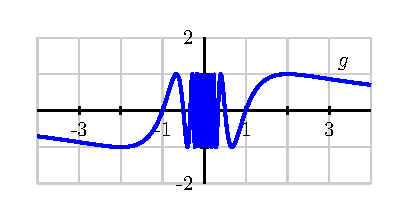
\includegraphics{figures/1_2_Ex1g.eps} 
%\end{tabular}
%\caption{Tables and graph for $\ds g(x) = \sin\left(\frac{\pi}{x}\right)$.} \label{F:1.2.Ex1g}
%\end{figure}

%First, as $x \to 3$, it appears from the data (and the graph) that the function is approaching approximately $0.866025$.  To be precise, we have to use the fact that $\frac{\pi}{x} \to \frac{\pi}{3}$, and thus we find that $g(x) = \sin(\frac{\pi}{x}) \to \sin(\frac{\pi}{3})$ as $x \to 3$.  The exact value of $\sin(\frac{\pi}{3})$ is $\frac{\sqrt{3}}{2}$, which is approximately 0.8660254038.  Thus, we see that
%$$\lim_{x \to 3} g(x) = \frac{\sqrt{3}}{2}.$$
%
%As $x \to 0$, we observe that $\frac{\pi}{x}$ does not behave in an elementary way.  When $x$ is positive and approaching zero, we are dividing by smaller and smaller positive values, and $\frac{\pi}{x}$ increases without bound.  When $x$ is negative and approaching zero, $\frac{\pi}{x}$ decreases without bound.  In this sense, as we get close to $x = 0$, the inputs to the sine function are growing rapidly, and this leads to wild oscillations in the graph of $g$.  It is an instructive exercise to plot the function $g(x) = \sin\left(\frac{\pi}{x}\right)$ with a graphing utility and then zoom in on $x = 0$.  Doing so shows that the function never settles down to a single value near the origin and suggests that $g$ does not have a limit at $x = 0$.

\end{example} % EXAMPLE

\begin{margintable}
\scalebox{1.15}{
\begin{tabular}{cc}
	\raisebox{-.05in}{
	\begin{tabular}[b]{r|l} 
	$x$ & $g(x)$ \\ 
	\hline 2.9 & 0.84864 \\ 
	2.99 & 0.86428 \\ 
	2.999 & 0.86585 \\ 
	2.9999 & 0.86601 \\ 
	3.1 & 0.88351 \\ 
	3.01 &  0.86777 \\ 
	3.001 & 0.86620 \\ 
	3.0001 &  0.86604 \\ 
	\end{tabular} } &	
	\raisebox{-.05in}{
	\begin{tabular}[b]{r|l} 
	$x$ & $g(x)$ \\ 
	\hline -0.1 & 0 \\ 
	-0.01 & 0 \\ 
	-0.001 & 0 \\ 
	-0.0001 & 0 \\ 
	0.1 & 0 \\ 
	0.01 & 0 \\ 
	0.001 & 0 \\ 
	0.0001 & 0 \\ 
	\end{tabular} } 
\end{tabular}
} % end scalebox
\caption{Tables for $\ds g(x) = \sin\left(\frac{\pi}{x}\right)$.} \label{T:1-1_Eg2}
\end{margintable}

\begin{marginfigure}
\margingraphics{figures/1_2_Ex1g.eps}
\caption{The graph of \newline $g(x)=\sin\left( \frac{\pi}{x} \right)$ near $3$ and $0$.}\label{fig:1-1_Eg2}
\end{marginfigure}

%	\hspace{0.25in} 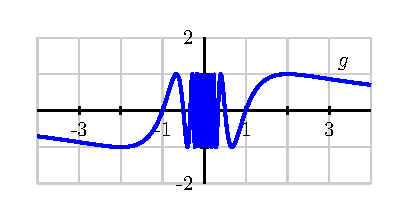
\includegraphics{figures/1_2_Ex1g.eps} 

\begin{example} \label{Ex:1.1.Eg2}
Use both tables and graphical approaches to investigate and, if possible, estimate or determine the value of the limit for the following function at the specified values. 
\[ \ds g(x) = \sin\left( \frac{\pi}{x} \right); \quad a = 3, \ a = 0\]

\solution Again, we construct two tables and a graph, see Table~\ref{T:1-1_Eg2} and Figure~\ref{fig:1-1_Eg2}.

First, as $x \to 3$, it appears from the data (and the graph) that the function is approaching approximately $0.866025$.  To be precise, we have to use the fact that $\frac{\pi}{x} \to \frac{\pi}{3}$, and thus we find that $g(x) = \sin(\frac{\pi}{x}) \to \sin(\frac{\pi}{3})$ as $x \to 3$.  The exact value of $\sin(\frac{\pi}{3})$ is $\frac{\sqrt{3}}{2}$, which is approximately 0.8660254038.  Thus, we see that
$$\lim_{x \to 3} g(x) = \frac{\sqrt{3}}{2}.$$

As $x \to 0$, we observe that $\frac{\pi}{x}$ does not behave in an elementary way.  When $x$ is positive and approaching zero, we are dividing by smaller and smaller positive values, and $\frac{\pi}{x}$ increases without bound.  When $x$ is negative and approaching zero, $\frac{\pi}{x}$ decreases without bound.  In this sense, as we get close to $x = 0$, the inputs to the sine function are growing rapidly, and this leads to wild oscillations in the graph of $g$.  It is an instructive exercise to plot the function $g(x) = \sin\left(\frac{\pi}{x}\right)$ with a graphing utility and then zoom in on $x = 0$.  Doing so shows that the function never settles down to a single value near the origin and suggests that $g$ does not have a limit at $x = 0$.
\end{example} % EXAMPLE

\begin{margintable}[6cm]
\begin{tabular}{c|c||c|c}
	$x$ & $f(x)$ & $x$ & $f(x)$ \\ \hline
	$0.5$ & $1.5$ & $1.5$ & \hspace{.75in} \\
	$0.9$ & \hspace{.75in} & $1.1$ & $2.1$ \\
	$0.99$ & $1.99$ & $1.01$ & \hspace{.75in} \\
	$0.999$ & \hspace{.75in} & $1.001$ & $2.001$ \\
\end{tabular}
\caption{Tabe of values near $x=1$.}
\label{T:1-1_Act1}
\end{margintable}

\begin{activity} \label{A:1.1.1}  Consider the function $f(x) = \dfrac{x^2 - 1}{x - 1}$.
\ba
\item Does the value of $f(1)$ exist? Why/why not?

\item Use a calculator or spreadsheet to fill in the blanks of Table~\ref{T:1-1_Act1}. Some of these have already been done for you; your calculations should not be drastically different from the ones already here. For example a calculation equal to 22.5 is very likely incorrect. Based on the table, estimate the value of $\ds \lim_{x \to 1} \frac{x^2 - 1}{x-1}$. 

\item Plot an accurate graph of the function $f$.  It should be a straight line.  Using your plot, what is $f(1)$?  What is $\ds \lim_{x \to 1} f(x)$?

\item Now use algebra to simplify the fraction $\dfrac{x^2 - 1}{x - 1}$. Call this new function $g(x)$.  What is $\ds \lim_{x \to 1} g(x)$? How is this limit related to the limit of $f(x)$ as $x$ approaches $1$?
\ea
\end{activity}

\aftera
 % ACTIVITY

An important lesson to take from Example~\ref{Ex:1.1.Eg2} is that both graphs and tables can be misleading when determining the value of a limit.  While a table of values is useful for investigating the possible value of a limit, we should also use other tools to confirm the value, if we think the table suggests the limit exists.

%-----------------------------------------------------------------------
% SUBSECTION IDENTIFYING WHEN LIMITS DO NOT EXIST
%-----------------------------------------------------------------------
\subsection{Identifying When Limits Do Not Exist}

As we have seen in Example~\ref{Ex:1.1.Eg2}, a function may not have a limit for all values of $x$. That is, we cannot say $\ds \lim_{x\to a}f(x)=L$ for some numbers $L$ for all values of $a$, for there may not be a number that $f(x)$ is approaching. There are three ways in which a limit may fail to exist. \index{limit!does not exist}
\begin{enumerate}[1)]
\item The function $f(x)$ may approach different values on either side of $a$.
\item The function may grow without upper or lower bound as $x$ approaches $a$.
\item The function may oscillate as $x$ approaches $a$, which we saw in Example~\ref{Ex:1.1.Eg2}.
\end{enumerate}

\begin{example} \label{Ex:1.1.Eg5}
Explore why $\ds \lim_{x\to 1} f(x)$ does not exist, where 
\[ f(x) = \left\{ \begin{array}{cl} x^2-2x+3 & x\leq 1 \\ x & x>1 \end{array} \right..\]

\solution A graph of $f(x)$ around $x=1$ is given in Figure~\ref{fig:1-1_Eg5}. It is clear that as $x$ approaches 1, $f(x)$ does not approach a single number. Instead, $f(x)$ approaches two different numbers. When considering values of $x$ less than 1 (approaching 1 from the left), $f(x)$ is approaching 2; when considering values of $x$ greater than 1 (approaching 1 from the right), $f(x)$ is approaching 1. Recognizing this behavior is important; we'll study this in greater depth later. Right now, it suffices to say that the limit does not exist since $f(x)$ is not approaching a single value as $x$ approaches 1.
\end{example}

\begin{marginfigure}[-8cm]
\margingraphics{figs/1/fignolimit1.pdf}
\caption{Observing no limit as $x\to 1$.}\label{fig:1-1_Eg5}
\end{marginfigure} % EXAMPLE

\begin{marginfigure}[1cm]
\margingraphics{figs/1/fignolimit2.pdf}
\caption{Observing no limit as $x \to 1$.}\label{fig:1-1_Eg6}
\end{marginfigure}

\begin{example} \label{Ex:1.1.Eg6}
Explore why $\ds \lim_{x\to 1} \frac{1}{(x-1)^2}$ does not exist.

\solution A graph of $\ds f(x) = \frac{1}{(x-1)^2}$ is given in Figure~\ref{fig:1-1_Eg6}. It shows that as $x$ approaches 1, $f(x)$ grows without bound in the positive direction. 

We can deduce this on our own, without the aid of the graph or table. If $x$ is near 1, then $(x-1)^2$ is very small, and: 
\[ \frac{1}{\text{very small number}} \rightarrow \text{very large number}.\]
Since $f(x)$ is not approaching a single number (growing without bound), we conclude that 
\[ \lim_{x \to 1} \frac{1}{(x-1)^2} \] 
does not exist.
\end{example} % EXAMPLE

%----------------------------------------------------------------------------
% SUBSECTION COMPUTING LIMITS
%----------------------------------------------------------------------------
\subsection{Computing Limits} 

Thus far, our method of finding a limit is making a really good approximation either graphically or numerically.  Later, we will cover the precise method of $\epsilon$--$\delta$ proofs\footnote{See Section~\ref{S:1.4.precise} for more on the precise definition of a limit.} which can be quite cumbersome. Now, we will cover a series of laws which allow us to find limits analytically. 

Suppose that $\ds \lim_{x\to 2} f(x)=2$ and $\ds \lim_{x\to 2} g(x) = 3$. What is \newline $\ds \lim_{x\to 2}(f(x)+g(x))$? Intuition tells us that the limit should be $5$, as we wish limits to behave in a nice way. The following concept states that already established limits do behave nicely.

\concept{Limit Laws}{\small % CONCEPT
Let $b$, $c$, $L$ and $K$ be real numbers, let $n$ be a positive integer, and let $f$ and $g$ be functions with the following limits: \index{limit!properties}
\[ \lim_{x \to c}f(x) = L \text{\ and\ } \lim_{x\to c} g(x) = K. \]
The following limits hold.
\begin{enumerate}[1)]
\item \parbox{80pt}{Constants:} $\ds \lim_{x\to c} b = b$
\item \parbox{80pt}{Identity: } $\ds \lim_{x\to c} x = c$
\item \parbox{80pt}{Sums/Differences:} $\ds \lim_{x\to c}(f(x)\pm g(x)) = L\pm K$
\item \parbox{80pt}{Scalar Multiples:}	$\ds \lim_{x\to c} b\cdot f(x) = bL$
\item \parbox{80pt}{Products:} $\ds \lim_{x\to c} f(x)\cdot g(x) = LK$
\item \parbox{80pt}{Quotients:} $\ds \lim_{x\to c} f(x)/g(x) = L/K$, ($K\neq 0)$
\item \parbox{80pt}{Powers:} 	$\ds \lim_{x\to c} f(x)^n = L^n$
\item \parbox{80pt}{Roots:} \parbox[t]{185pt}{$\ds \lim_{x\to c} \sqrt[n]{f(x)} = \sqrt[n]{L}$ \qquad \small (if $n$ is even then $L$ must be greater than $0$.)}
\item \parbox{80pt}{Compositions:} \parbox[t]{200pt}{Adjust our previously given limit situation to: 
\[ \lim_{x\to c}f(x) = L \text{\ and\ } \lim_{x\to L} g(x) = K.\] 
Then $\ds \lim_{x\to c}g(f(x)) = K$.}
\end{enumerate}
} % end concept

\begin{example} \label{Ex:1.1.Eg3}
Let $\ds \lim_{x\to 2} f(x)=2$, $\ds  \lim_{x\to 2} g(x) = 3$ and $\ds p(x) = 3x^2-5x+7$. Find the following limits:

\begin{enumerate}[1)]
\item $\ds \lim_{x\to 2} \big(f(x) + g(x)\big)$
\item $\ds \lim_{x\to 2} \big(5f(x) + g(x)^2\big)$
\item $\ds \lim_{x\to 2} p(x)$
\end{enumerate}

\solution

\begin{enumerate}[1)]
\item Using the Sum/Difference rule, we know that \newline $\ds \lim_{x\to 2} \big(f(x) + g(x)\big) = 2+3 =5$.
\item Using the Scalar Multiple, Sum/Difference, and Power rules, we find that $\ds \lim_{x\to 2} \big(5f(x) + g(x)^2\big) = 5\cdot 2 + 3^2 = 19.$
\item Here we combine the Power, Scalar Multiple, Sum/Difference and Constant Rules. We show quite a few steps, but in general these can be omitted:
\begin{align*}
\lim_{x\to 2} p(x) &= \lim_{x\to 2} (3x^2-5x+7) \\
&= \lim_{x\to 2} 3x^2-\lim_{x\to 2} 5x+\lim_{x\to 2}7 \\
&= 3\cdot 2^2 - 5\cdot 2+7 \\
&= 9
\end{align*}
\end{enumerate}
\end{example} %EXAMPLE

Notice that in the last part of the previous example, we have
\[ \lim_{x \to 2} p(x) = p(2) = 9,\]
meaning that we could have evaluated the limit simply by directly substituting the value of $a$ into the function.  That is possible because the function $p(x)$ is {\em continuous}\sidenote{See Section~\ref{S:1.3.Continuity} for more on the notion of continuity.}, which means that the limit of the function at any point is equal to its function value.

From Example~\ref{Ex:1.1.Eg1}, we can evaluate the limit $\ds \lim_{x \to -1} \frac{4-x^2}{x+2}$ by evaluating the function at $x = -1$:
\[ \lim_{x \to -1} \frac{4-x^2}{x+2} = \frac{4 - (-1)^2}{-1 + 2} = \frac{4-1}{1} = 3. \]
Or from Example~\ref{Ex:1.1.Eg2}, we can evaluate the limit $\ds \lim_{x \to 3} \sin \left( \frac{\pi}{x} \right)$ by evaluating the function at $x = 3$:
\[ \lim_{x \to 3} \sin \left( \frac{\pi}{x} \right) = \sin \left( \frac{\pi}{3} \right) = \frac{\sqrt{3}}{2}. \]
This method is quite important and is stated again for emphasis.

\concept{Direct Substitution} % CONCEPT
{If $f$ is a continuous function and $a$ is in the domain of $f$, then 
\[ \lim_{x \to a} f(x) = f(a) \] 
} %end concept

For $f(x)$ in Example~\ref{Ex:1.1.Eg1}, the situation is more complicated when $x \to -2$ since $f(-2)$ is not defined.  If we attempt to evaluate the limit using direct substitution, we observe that 
\[ \lim_{x \to -2} \frac{4-x^2}{x+2} = \frac{4 - (-2)^2}{-2 + 2} = \frac{4-4}{-2+2} = \frac{0}{0}. \]
We call $0/0$ an \emph{indeterminate form}\index{indeterminate}, or mathematical gibberish, and it tells us nothing about the limit---it could exist, it could not exist, we just don't know.  We simply observe that it tells us there is somehow more work to do.  From the table and graph of Example~\ref{Ex:1.1.Eg1}, it appears that $f$ should have a limit of $4$ at $x = -2$.  To see algebraically why this is the case, let's work directly with the form of $f(x)$.  Observe that
\begin{eqnarray*}
\lim_{x \to -2} f(x) & = & \lim_{x \to -2} \frac{4-x^2}{x+2} \\
& = & \lim_{x \to -2} \frac{(2-x)(2+x)}{x+2}. \\
\end{eqnarray*}
At this point, it is important to observe that since we are taking the limit as $x \to -2$, we are considering $x$ values that are close, but not equal, to $-2$.  Since we never actually allow $x$ to equal $-2$, the quotient $\frac{2+x}{x+2}$ has value 1 for every possible value of $x$.  Thus, we can simplify the most recent expression above, and now find that
\[ \lim_{x \to -2} \frac{4-x^2}{x+2} = \lim_{x \to -2} \frac{(2-x)(2+x)}{x+2} = \lim_{x \to -2} (2-x). \]
Because $2-x$ is simply a linear function, this limit is now easy to determine, and its value clearly is $4$.  Thus, from several points of view we've seen that $\ds\lim_{x \to -2} f(x) = 4.$

\begin{activity} \label{A:1.1.2}  Determine the exact value of the limit by using algebra to simplify the function. 
\ba
		\item $\ds \lim_{x \to -5} \frac{x^2 - 25}{x+5}$
		\item $\ds \lim_{x \to 0} \frac{(2+x)^3 - 8}{x}$
		\item $\ds \lim_{x \to 0} \frac{\sqrt{x+1} - 1}{x}$
\ea
\end{activity}
\begin{smallhint}
\ba
	\item $(x^2 - 25)$ can be factored.
	\item Expand the expression $(2+x)^3$, and then combine like terms in the numerator.
	\item Try multiplying the given function by this fancy form of 1: $\frac{\sqrt{x+1} + 1}{\sqrt{x+1} + 1}$.
\ea
\end{smallhint}
\begin{bighint}
\ba
	\item $(x^2 - 25) = (x+5)(x-5)$.
	\item Expand the expression $(2+x)^3$ using the rule $(a+b)^3 = a^3 + 3a^2b + 3ab^2 + b^3$, and then combine like terms in the numerator.
	\item Try multiplying the given function by this fancy form of 1: $\frac{\sqrt{x+1} + 1}{\sqrt{x+1} + 1}$.  Expand and simplify the numerator, and then see what happens as $x \to 0$.
\ea
\end{bighint}
\begin{activitySolution}
Estimating the values of the limits with tables is straightforward and should suggest the exact values stated below.
\ba
	\item $\ds \lim_{x \to 1} \frac{x^2 - 1}{x-1} = \lim_{x \to 1} \frac{(x+1)(x-1)}{x-1} = \lim_{x \to 1} (x+1) = 2$. 
	\item $\ds \lim_{x \to 0} \frac{(2+x)^3 - 8}{x} = \lim_{x \to 0} \frac{8 + 12x + 6x^2 + x^3 - 8}{x} = \lim_{x \to 0} \frac{12x + 6x^2 + x^3}{x} =  \lim_{x \to 0} (12 + 6x + x^2) = 12$.
	\item $\ds \lim_{x \to 0} \frac{\sqrt{x+1} - 1}{x} = \lim_{x \to 0} \frac{\sqrt{x+1} - 1}{x} \cdot \frac{\sqrt{x+1} + 1}{\sqrt{x+1} + 1} = \lim_{x \to 0} \frac{x+1-1}{x(\sqrt{x+1}+1)} = \lim_{x \to 0} \frac{1}{\sqrt{x+1}+1} = \frac{1}{2}.$
\ea
\end{activitySolution}
\aftera
 % ACTIVITY

The section could have been titled ``Using Known Limits to Find Unknown Limits.'' By knowing certain limits of functions, we can find limits involving sums, products, powers, etc., of these functions. We further the development of such comparative tools with the Squeeze Theorem, a clever and intuitive way to find the value of some limits. 

Suppose we have functions $f$, $g$ and $h$ where $g$ always takes on values between $f$ and $h$; that is, for all $x$ in an interval, 
\[ f(x) \leq g(x) \leq h(x). \] 
If $f$ and $h$ have the same limit at $c$, and $g$  is always ``squeezed'' between them, then $g$ must have the same limit as well. That is what the Squeeze Theorem states.

\concept{Squeeze Theorem} % CONCEPT
{Let $f$, $g$ and $h$ be functions on an open interval $I$ containing $c$ such that for all $x$ in $I$, $f(x)\leq g(x) \leq h(x)$. If 
\[ \lim_{x\to c} f(x) = L = \lim_{x\to c} h(x),\] 
then 
\[ \lim_{x\to c} g(x) = L.\] \index{limit!Squeeze Theorem}\index{Squeeze Theorem}
} % end concept

It can take some work to figure out appropriate functions by which to ``squeeze'' the given function you are trying to evaluate a limit of. However, that is generally the only place work is necessary; the theorem makes the ``evaluating the limit part'' very simple. %We use the Squeeze Theorem in the following example to prove that $\ds \lim_{x\to 0} \frac{\sin(x)}{x} = 1$.

\begin{example}\label{Ex:1.1.Eg9}
Given $4x-9 \leq f(x) \leq x^2-4x+7$, use the Squeeze Theorem to find $\ds \lim_{x \to 4} f(x)$.

\solution We begin by finding $\ds \lim_{x \to 4} (4x-9)$ and \newline $\ds \lim_{x \to 4} (x^2-4x+7)$. 
\[ \lim_{x \to 4} (4x-9) = 4(4)-9 = 7 \]
and 
\[ \lim_{x \to 4} (x^2-4x+7) = (4)^2-4(4)+7 = 7. \]
Therefore,
\[ \lim_{x \to 4} (4x-9) = 7 = \lim_{x \to 4} (x^2-4x+7),\]
and by the Squeeze Theorem, $\ds \lim_{x \to 4} f(x) = 7$.
\end{example} % EXAMPLE

\begin{activity}  \label{A:1.1.5}
In this activity, we prove $\ds \lim_{\theta \to 0} \frac{\sin(\theta)}{\theta} = 1$ using the squeeze theorem.  
\ba
	\item Draw the part of the unit circle that lies in the first quadrant. Place a point on the circle in the first quadrant and label it $(x,y)$.
	\item Draw the line connecting the origin to the point $(x,y)$ on the same graph. Label the angle between the line and the $x-axis$ as $\theta$.
	\item Find the area of the sector of the unit circle subtended by $\theta$ that you drew above.
	\item Draw a vertical line from the point $(x,y)$ to the $x$-axis. This will form a right triangle. \label{small}
	\item Find the area of the triangle in (\ref{small}) in terms of $\theta$. You will need to use trig functions. 
	\item Draw a line on the picture connecting the points $(1,0)$ and $(1,1)$. This will also form a right triangle. \label{large}
	\item Find the area of the triangle in (\ref{large}). You will need to use trig functions.
	\item What is the relationship between the three areas you found? Write this as an inequality.
	\item Write this inequality so that it involves the function $\frac{\sin(\theta)}{\theta}$.
	\item Now apply the squeeze theorem to get the result.
\ea
\end{activity}

%\begin{marginfigure}
%\margingraphics{figs/1/figSqueeze1.pdf}
%\caption{The unit circle and related triangles.}\label{fig:1-1_Eg4}
%\end{marginfigure}

\begin{activitySolution}
	We begin by considering the unit circle. Each point on the unit circle has coordinates $(\cos (\theta),\sin (\theta))$ for some angle $\theta$ as shown in Figure~\ref{fig:1-1_Eg4}. Using similar triangles, we can extend the line from the origin through the point to the point $(1,\tan (\theta))$, as shown. (Here we are assuming that $0 \leq \theta \leq \pi/2$. Later we will show that we can also consider $\theta \leq 0$.)

The area of the large triangle is $\frac{1}{2} \tan(\theta)$; the area of the sector is $\theta/2$; the area of the triangle contained inside the sector is $\frac{1}{2} \sin(\theta)$. It is then clear from the diagram that 
\[ \frac{\tan (\theta)}{2} \geq \frac{\theta}{2} \geq \frac{\sin (\theta)}{2}.\]

Multiply all terms by $\ds \frac{2}{\sin(\theta)}$, giving 
\[ \frac{1}{\cos(\theta)} \geq \frac{\theta}{\sin (\theta)} \geq 1.\]

Taking reciprocals reverses the inequalities, giving 
\[ \cos (\theta) \leq \frac{\sin(\theta)}{\theta} \leq 1.\]
These inequalities hold for all values of $\theta$ near 0, even negative values, since $\cos (-\theta) = \cos(\theta)$ and $\sin (-\theta) = -\sin (\theta)$.

Now take the limit of everything as $\theta \to 0$.

\[ \lim_{\theta \to 0} \cos (\theta) \leq \lim_{\theta \to 0} \frac{\sin(\theta)}{\theta} \leq \lim_{\theta \to 0}  1 \]
\[ \cos 0 \leq \lim_{\theta \to 0} \frac{\sin(\theta)}{\theta} \leq  1 \]
\[ 1 \leq \lim_{\theta \to 0} \frac{\sin(\theta)}{\theta} \leq  1 \]

By the Squeeze Theorem, $\ds \lim_{\theta \to 0} \frac{\sin(\theta)}{\theta}=1$.
\end{activitySolution}
\aftera
 % ACTIVITY

%------------------------------------------
% SUBSECTION ONE-SIDED LIMITS
%------------------------------------------
\subsection*{One-Sided Limits}

In this section, we explored the three ways in which limits of functions failed to exist: 
\begin{enumerate}[1)]
\item The function approached different values from the left and right,
\item The function grows without bound, and 
\item The function oscillates as $x$ approaches $a$.
\end{enumerate}
	
Now we explore in depth the concepts behind item \#1 by introducing the \textit{one-sided limit}. We begin with  definitions that are very similar to the definition of the limit given earlier, but the notation is slightly different.

\definition{One-Sided Limits}{ % DEFINTION
\textbf{Left-Sided Limit:} \index{limit!one sided}\index{limit!right sided}\index{limit!left sided} Let $f$ be a function defined on an open interval containing $a$. The notation 
\[ \lim_{x \to a^-} f(x) = L \] 
is read as ``the limit of $f(x)$ as $x$ approaches $a$ from the left is $L$,'' or ``the \textit{left-sided limit of $f$ at $a$ is L}''.\\

\noindent\textbf{Right-Sided Limit:} Let $f$ be a function defined on an open interval containing $a$. The notation 
\[ \lim_{x \to a^+} f(x) = L \] 
is read as ``the limit of $f(x)$ as $x$ approaches $a$ from the right is $L$,'' or ``the \textit{right-sided limit of $f$ at $a$ is L}''.
} % end definition

Practically speaking, when evaluating a left-hand limit, we consider only values of $x$ ``to the left of $a$,'' i.e., where $x<a$. The admittedly imperfect notation $x \to a^-$ is used to imply that we look at values of $x$ to the left of $a$. The notation has nothing to do with positive or negative values of either $x$ or $a$. 

A similar statement holds for evaluating right-hand limits; there we consider only values of $x$ to the right of $a$, i.e., $x>a$. We can use the Limit Laws given earlier to help us evaluate these limits; we just restrict our view to one side of $a$.

\begin{marginfigure}[8cm]
\margingraphics{figs/1/figOneSidedLimits1.pdf}
\caption{The graph of $f$.}\label{fig:1-1_Eg7}
\end{marginfigure}

%\mfigure{.7}{A graph of $f$ in Example \ref{ex_onesidea}.}{fig:onesided1}{figures/figOneSidedLimits1}}

\begin{example} \label{Ex:1.1.Eg7}
Let $\ds f(x) = \left\{\begin{array}{cc} x & 0\leq x\leq 1 \\ 3-x & 1<x<2\end{array},\right.$ as shown in Figure~\ref{fig:1-1_Eg7}. Find each of the following: 
\begin{multicols}{2}
\begin{enumerate}[1)]
\item		$\ds \lim_{x\to 1^-} f(x)$
\item		$\ds \lim_{x\to 1^+} f(x)$
\item		$\ds \lim_{x\to 1} f(x)$
\item		$\ds f(1)$
\item		$\ds \lim_{x\to 0^+} f(x)$
\item		$f(0)$
\item		$\ds \lim_{x\to 2^-} f(x)$
\item		$f(2)$
\end{enumerate}
\end{multicols}

\solution For these problems, the visual aid of the graph is likely more effective in evaluating the limits than using $f$ itself. Therefore we will refer often to the graph.
\begin{enumerate}[1)]
\item As $x$ goes to $1$ \textit{from the left}, we see that $f(x)$ is approaching the value of $1$. Therefore $\ds \lim_{x\to 1^-} f(x) =1.$

\item As $x$ goes to $1$ \textit{from the right}, we see that $f(x)$ is approaching the value of $2$. Recall that it does not matter that there is an ``open circle'' there; we are evaluating a limit, not the value of the function. Therefore $\ds \lim_{x\to 1^+} f(x)=2$.

\item The limit of $f$ as $x$ approaches $1$ does not exist, as discussed earlier. The function does not approach one particular value, but two different values from the left and the right.

\item Using the definition and by looking at the graph we see that $f(1) = 1$.

\item As $x$ goes to $0$ from the right, we see that $f(x)$ is also approaching $0$. Therefore $\ds \lim_{x\to 0^+} f(x)=0$. Note we cannot consider a left-hand limit at $0$ as $f$ is not defined for values of $x<0$.

\item Using the definition and the graph, $f(0) = 0$.

\item As $x$ goes to $2$ from the left, we see that $f(x)$ is approaching the value of $1$. Therefore $\ds \lim_{x\to 2^-} f(x)=1.$

\item The graph and the definition of the function show that $f(2)$ is not defined.
\end{enumerate}
\end{example}


 % EXAMPLE

Note how the left and right-hand limits were different; this, of course, causes the two-sided limit to not exist. The following theorem states what is fairly intuitive: the two-sided limit exists precisely when the left and right-hand limits are equal.

\concept{Limits and One Sided Limits} % CONCEPT
{Let $f$ be a function defined on an open interval $I$ containing $a$. \index{limit!does not exist} Then 
\[ \lim_{x \to a}f(x) = L\] 
if, and only if, 
\[ \lim_{x \to a^-}f(x) = L \quad \text{and} \quad \lim_{x \to a^+}f(x) = L.\]
} % end concept

The phrase ``if, and only if'' means the two statements are \textit{equivalent}: they are either both true or both false. If the limit equals $L$, then the left and right hand limits both equal $L$. If the limit is not equal to $L$, then at least one of the left and right-hand limits is not equal to $L$ (it may not even exist).

One thing to consider is that the value of the function may/may not be equal to the value(s) of its left/right-hand limits, even when these limits agree.

\begin{marginfigure}[8cm]
\margingraphics{figs/1/figOneSidedLimits3.pdf}
\caption{The graph of $f$.}\label{fig:1-1_Eg8}
\end{marginfigure}

\begin{example} \label{Ex:1.1.Eg8}
Let $f(x) = \left\{\begin{array}{cc} (x-1)^2 & 0\leq x\leq 2, x\neq 1\\ 1 & x=1\end{array},\right.$ as shown in Figure~\ref{fig:1-1_Eg8}. Evaluate the following.
\begin{multicols}{2}
\begin{enumerate}[1)]
\item $\ds \lim_{x\to 1^-} f(x)$
\item $\ds \lim_{x\to 1^+} f(x)$
\item $\ds \lim_{x\to 1} f(x)$
\item $f(1)$
\end{enumerate}
\end{multicols}

\solution It is clear by looking at the graph that both the left and right-hand limits of $f$, as $x$ approaches $1$, is $0$. Thus it is also clear that the limit is $0$; i.e., $\ds \lim_{x\to 1} f(x) = 0$. It is also clearly stated that $f(1) = 1$.
\end{example} % EXAMPLE

This concludes a rather lengthy introduction to the notion of limits.  It is important to remember that our primary motivation for considering limits of functions comes from our interest in studying the rate of change of a function.  To that end, we close this section by revisiting our previous work with average and instantaneous velocity and highlighting the role that limits play. 

%-----------------------------------------------------
% SUBSECTION INSTANTANEOUS VELOCITY
%-----------------------------------------------------
\subsection*{Instantaneous Velocity}

Suppose that we have a moving object whose position at time $t$ is given by a function $s$.  We know that the average velocity of the object on the time interval $[a,b]$ is $AV_{[a,b]} = \frac{s(b)-s(a)}{b-a}.$  We define the \emph{instantaneous velocity} \index{instantaneous velocity} at $a$ to be the limit of average velocity as $b$ approaches $a$.  Note particularly that as $b \to a$, the length of the time interval gets shorter and shorter (while always including $a$).  In Section~\ref{S:2.1.DerivativePt}, we will introduce a helpful shorthand notation to represent the instantaneous rate of change.  For now, we will write $IV_{t=a}$ for the instantaneous velocity at $t = a$, and thus
$$IV_{t=a} = \lim_{b \to a} AV_{[a,b]} = \lim_{b \to a} \frac{s(b)-s(a)}{b-a}.$$
Equivalently, if we think of the changing value $b$ as being of the form $b = a + h$, where $h$ is some small number, then we may instead write
$$IV_{t=a} = \lim_{h \to 0} AV_{[a,a+h]} = \lim_{h \to 0} \frac{s(a+h)-s(a)}{h}.$$
Again, the most important idea here is that to compute instantaneous velocity\index{instantaneous velocity}, we take a limit of average velocities as the time interval shrinks.  Two different activities offer the opportunity to investigate these ideas and the role of limits further. \\

\begin{activity}  \label{A:1.1.3}
Consider a moving object whose position function is given by $s(t) = t^2$, where $s$ is measured in meters and $t$ is measured in minutes.  
\ba
	\item Determine the most simplified expression for the average velocity of the object on the interval $[3, 3+h]$, where $h > 0$.
	\item Determine the average velocity of the object on the interval $[3,3.2]$.  Include units on your answer.
	\item Determine the instantaneous velocity of the object when $t = 3$.  Include units on your answer.
\ea
\end{activity}
\begin{smallhint}
\ba
	\item $s(3+h) = (3+h)^2$.
	\item Recall that $AV_{[a,b]} = \frac{s(b)-s(a)}{b-a}$.
	\item Consider $\lim_{h \to 0} \frac{s(3+h)-s(3)}{h}$ and use your work in (a).
\ea
\end{smallhint}
\begin{bighint}
\ba
	\item $s(3+h) = (3+h)^2 = 9 + 6h + h^2$; show that $s(3+h) - s(3) = 6h + h^2$.
	\item Compute $AV_{[3,3.2]} = \frac{s(3.2)-s(3)}{3.2-3}$.
	\item Consider $\lim_{h \to 0} \frac{s(3+h)-s(3)}{h} = \lim_{h \to 0} \frac{6h + h^2}{h}$.
\ea
\end{bighint}
\begin{activitySolution}
\ba
	\item Observe that $AV_{[3, 3+h]} =  \frac{s(3+h)-s(3)}{h} = \frac{(3+h)^2 - 3^2}{h} = \frac{9 + 6h + h^2 - 9}{h} = \frac{6h + h^2}{h} = \frac{h(6 + h)}{h} = 6 + h.$
	\item Using the expression just found in (a) with $h = 0.2$, $AV_{[3,3.2]} = 6 + 0.2 = 6.2$ meters/min.
	\item Taking the limit of average velocity and using our work from (a), we find that
	$$IV_{t = 3} = \lim_{h \to 0} AV_{[3, 3+h]} = \lim_{h \to 0} 6+h = 6,$$
	so the instantaneous velocity of the object when $t = 3$ is 6 meters per minute.
\ea
\end{activitySolution}
\aftera
 % ACTIVITY

The closing activity of this section asks you to make some connections among average velocity, instantaneous velocity, and slopes of certain lines.
\newpage
\begin{marginfigure}
\margingraphics{figures/1_2_Act3.eps} 
\caption{Plot of the position function $y = s(t)$ in Activity~\ref{A:1.1.4}.}
\end{marginfigure}

\begin{activity} \label{A:1.1.4}
For the moving object whose position $s$ at time $t$ is given by the graph below, answer each of the following questions.  Assume that $s$ is measured in feet and $t$ is measured in seconds.

\ba
	\item Use the graph to estimate the average velocity of the object on each of the following intervals: $[0.5,1]$, $[1.5,2.5]$, $[0,5]$.  Draw each line whose slope represents the average velocity you seek.
	\item How could you use average velocities or slopes of lines to estimate the instantaneous velocity of the object at a fixed time?
	\item Use the graph to estimate the instantaneous velocity of the object when $t = 2$.  Should this instantaneous velocity at $t = 2$ be greater or less than the average velocity on $[1.5,2.5]$ that you computed in (a)?  Why?
\ea
\end{activity} 
\begin{smallhint}
\ba
	\item Remember that average velocity on an interval computes the quotient of ``change in $s$ over change in $t$.''  This is the slope of the line between the corresponding two points on the graph of $s$.
	\item Think about shorter and shorter time intervals and drawing the lines whose slopes represent average velocity.
	\item Think about zooming in on the graph at $t = 2$ and drawing a line that, up close, looks just like the curve $s(t)$.  What is the approximate slope of that line?
\ea
\end{smallhint}
\begin{bighint}
\ba
	\item Remember that average velocity on an interval computes the quotient of ``change in $s$ over change in $t$.''  This is the slope of the line between the corresponding two points on the graph of $s$.  For example, the average velocity on $[0.5,1]$ is $\frac{1-1}{1-0.5} = 0$.
	\item Think about shorter and shorter time intervals and drawing the lines whose slopes represent average velocity.  If those lines' slopes are approaching a single number, that number represents the instantaneous velocity.
	\item Think about zooming in on the graph at $t = 2$ and drawing a line that, up close, looks just like the curve $s(t)$.  What is the approximate slope of that line?  By drawing this line that looks like $s(t)$ near the point $(2,s(2))$ and comparing the line through the points $(1.5,s(1.5))$ and $(2.5, s(2.5))$, you should be able to compare the lines and see which has greater slope.
\ea
\end{bighint}
\begin{activitySolution}
\ba
	\item The average velocity on $[0.5,1]$ is the slope of the line joining the points $(0.5,s(0.5))$ and $(1,s(1))$, which is $AV_{[0.5,1]} = \frac{1-1}{1-0.5} = 0$.  On $[1.5,2.5]$, we similarly find $AV_{[1.5,2.5]} = \frac{3-1}{2.5-1.5} = 2$, and on $[0,5]$, we have $AV_{[0,5]} = \frac{5-0}{5-0} = 1$.
	\item  Take shorter and shorter time intervals and draw the lines whose slopes represent average velocity.  If those lines' slopes are approaching a single number, that number represents the instantaneous velocity.  For example, to estimate the instantaneous velocity at $t = 2$, we might consider average velocities on $[2,3]$, $[2,2.5]$, and $[2,2.25]$.
	\item  If we draw the line through $(2,2)$ and $(2.1,s(2.1))$, it looks like the line's slope is approximately 2.5: if we go over one grid-width, we appear to go up about 2.5.  The slope of this line is clearly greater than the slope of the line through $(1.5, s(1.5))$ and $(2.5, s(2.5))$, which is 2. Hence the instantaneous velocity at $t = 2$ is greater than the average velocity on $[1.5,2.5]$.
\ea
\end{activitySolution}
\aftera
 % ACTIVITY

%\begin{authornote}
%This is an author note.
%\end{authornote}

%--------------
% SUMMARY
%--------------
\begin{summary}
\item Limits enable us to examine trends in function behavior near a specific point.  In particular, taking a limit at a given point asks if the function values nearby tend to approach a particular fixed value.

\item When we write $\ds \lim_{x \to a} f(x) = L$, we read this as saying ``the limit of $f$ as $x$ approaches $a$ is $L$,'' and this means that we can make the value of $f(x)$ as close to $L$ as we want by taking $x$ sufficiently close (but not equal) to $a$.

\item If we desire to know $\ds \lim_{x \to a} f(x)$ for a given value of $a$ and a known function $f$, we can estimate this value from the graph of $f$ or by generating a table of function values that result from a sequence of $x$-values that are closer and closer to $a$.  If we want the exact value of the limit, we need to work with the function algebraically and see if we can use familiar properties of known, basic functions to understand how different parts of the formula for $f$ change as $x \to a$. 

\item The instantaneous velocity of a moving object at a fixed time is found by taking the limit of average velocities of the object over shorter and shorter time intervals that all contain the time of interest.
\end{summary}

\clearpage

%--------------
% EXERCISES
%--------------
\begin{adjustwidth*}{}{-2.25in}
\textbf{{\large Exercises}}
\setlength{\columnsep}{25pt}
\begin{multicols*}{2}
\noindent Terms and Concepts \small

\begin{enumerate}[1)]
\item In your own words, what does it mean to ``find the limit of $f(x)$ as $x$ approaches 3''?
\item An expression of the form $\frac00$ is called \underline{\hskip 15pt}.
\item T/F: The limit of $f(x)$ as $x$ approaches $5$ is always $f(5)$.
\item T/F: If $\ds \lim_{x\to 1^-} f(x) = 5$, then $\ds \lim_{x\to 1} f(x) = 5$.
\item T/F: If $\ds \lim_{x\to 1^-} f(x) = 5$, then $\ds \lim_{x\to 1^+} f(x) = 5$.
\item T/F: If $\ds \lim_{x\to 1} f(x) = 5$, then $\ds \lim_{x\to 1^-} f(x) = 5$.
\item Describe three situations where $\displaystyle \lim_{x\to c}f(x)$ does not exist.
\end{enumerate} 

\noindent {\normalsize Problems\\} \small

\noindent In the following exercises, evaluate each expression using the given graph of $f(x)$.

\begin{enumerate}[1),resume]
\item 
\begin{minipage}{\linewidth}\centering
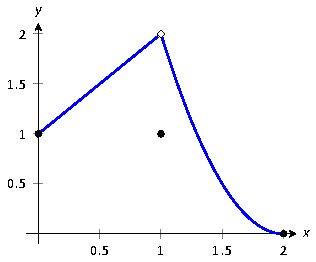
\includegraphics[scale=.8]{figures/fig01_04_ex_05}
\end{minipage}

\noindent\begin{minipage}[t]{.5\linewidth}
\begin{enumerate}
\item		$\ds \lim_{x\to 1^-} f(x)$
\item		$\ds \lim_{x\to 1^+} f(x)$
\item		$\ds \lim_{x\to 1} f(x)$
\end{enumerate}
\end{minipage}
\noindent\begin{minipage}[t]{.5\linewidth}
\begin{enumerate}\addtocounter{enumii}{3}
\item		$f(1)$
\item		$\ds \lim_{x\to 0^-} f(x)$
\item		$\ds \lim_{x\to 0^+} f(x)$
\end{enumerate}
\end{minipage}

\item
\begin{minipage}{\linewidth}\centering
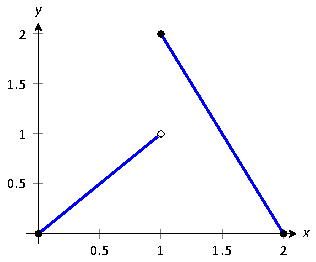
\includegraphics[scale=.8]{figures/fig01_04_ex_06}
\end{minipage}

\noindent\begin{minipage}[t]{.5\linewidth}
\begin{enumerate}
\item		$\ds \lim_{x\to 1^-} f(x)$
\item		$\ds \lim_{x\to 1^+} f(x)$
\item		$\ds \lim_{x\to 1} f(x)$
\end{enumerate}
\end{minipage}
\noindent\begin{minipage}[t]{.5\linewidth}
\begin{enumerate}\addtocounter{enumii}{3}
\item		$f(1)$
\item		$\ds \lim_{x\to 2^-} f(x)$
\item		$\ds \lim_{x\to 2^+} f(x)$
\end{enumerate}
\end{minipage}

\item
\begin{minipage}{\linewidth}\centering
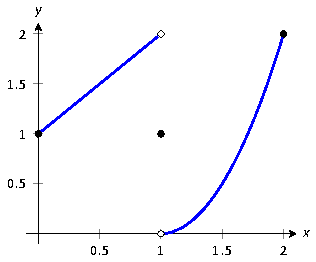
\includegraphics[scale=.8]{figures/fig01_04_ex_08}
\end{minipage}

\noindent\begin{minipage}[t]{.5\linewidth}
\begin{enumerate}
\item		$\ds \lim_{x\to 1^-} f(x)$
\item		$\ds \lim_{x\to 1^+} f(x)$
\end{enumerate}
\end{minipage}
\noindent\begin{minipage}[t]{.5\linewidth}
\begin{enumerate}\addtocounter{enumii}{2}
\item		$\ds \lim_{x\to 1} f(x)$
\item		$f(1)$
%\item		$\ds \lim_{x\to 2^-} f(x)$
%\item		$\ds \lim_{x\to 0^+} f(x)$
\end{enumerate}
\end{minipage}

\end{enumerate}

\vspace{.5cm}

\noindent Using:

\begin{tabular}{lll}
$\ds \lim_{x \to 9}f(x) = 6$ & \quad\quad &$\ds \lim_{x \to 6} f(x) = 9$\\
$\ds \lim_{x \to 9}g(x) = 3$ &  & $\ds \lim_{x \to 6} g(x) = 3$
\end{tabular}

\noindent evaluate the limits given in the following exercises, where possible. If it is not possible to know, state so.
\begin{enumerate}[1),resume]
\item $\ds \lim_{x\to9}(f(x)+g(x))$
\item $\ds \lim_{x\to9}(3f(x)/g(x))$
\item $\ds \lim_{x\to9}\left(\frac{f(x)-2g(x)}{g(x)}\right)$
\item $\ds \lim_{x\to6}\left(\frac{f(x)}{3-g(x)}\right)$
\item $\ds \lim_{x\to9}g\big(f(x)\big)$
\item $\ds \lim_{x\to6}f\big(g(x)\big)$
\item $\ds \lim_{x\to6}g\big(f(f(x))\big)$
\item $\ds \lim_{x\to6}f(x)g(x)-f\,^2(x)+g^2(x)$
\end{enumerate}

\vspace{.5cm}

\noindent Using:

\begin{tabular}{lll}
$\ds \lim_{x\to1}f(x) = 2$ & \quad\quad &$\ds \lim_{x\to10} f(x) = 1$\\
$\ds \lim_{x\to1}g(x) = 0$ &  & $\ds \lim_{x\to10} g(x) = \pi$
\end{tabular}

\noindent evaluate the limits given in the following exercises, where possible. If it is not possible to know, state so.
\begin{multicols}{2}
\begin{enumerate}[1),resume]
\item $\ds \lim_{x\to1}f(x)^{g(x)}$
\item $\ds \lim_{x\to10}\cos \big(g(x)\big)$
\item $\ds \lim_{x\to1}f(x)g(x)$
\item {$\ds \lim_{x\to1}g\big(5f(x)\big)$}
\end{enumerate}
\end{multicols}

\vspace{.5cm}

\noindent In the following exercises, evaluate the limit.
\begin{multicols}{2}
\begin{enumerate}[1),start=23]
\item {$\ds \lim_{x\to3}x^2-3x+7$}
\item {$\ds \lim_{x\to\pi}\frac{3x+1}{1-x}$}
\item {$\ds \lim_{x\to\pi}\frac{x^2+3x+5}{5x^2-2x-3}$}
\item {$\ds \lim_{x\to\pi}\left(\frac{x-3}{x-5}\right)^7$}
\item {$\ds \lim_{x\to\pi/4}\cos x\sin x$}
\item {$\ds \lim_{x\to0}\ln x$}
\end{enumerate}
\end{multicols}

%------------------------------------------
% END OF EXERCISES ON FIRST PAGE
%------------------------------------------
\end{multicols*}
\end{adjustwidth*}

\clearpage

\begin{adjustwidth*}{}{-2.25in}
\setlength{\columnsep}{25pt}
\begin{multicols*}{2}\small

\begin{multicols}{2}
\begin{enumerate}[1),start=29]
\item {$\ds \lim_{x\to3}4^{x^3-8x}$}
\item {$\ds \lim_{x\to\pi/6} \csc x$}
\item {$\ds \lim_{x\to0} \ln(1+x)$}
\item {$\ds \lim_{x\to6^-} \frac{x^2-4 x-12}{x^2-13 x+42}$}
\item {$\ds \lim_{x\to0^+} \frac{x^2+2 x}{x^2-2 x}$}
\item {$\ds \lim_{x\to2^-} \frac{x^2+6 x-16}{x^2-3 x+2}$}
\item {$\ds \lim_{x\to2^+}\frac{x^2-10 x+16}{x^2-x-2}$}
\item {$\ds \lim_{x\to-2}\frac{x^2-5 x-14}{x^2+10 x+16}$}
\item {$\ds \lim_{x\to-1}\frac{x^2+9 x+8}{x^2-6 x-7}$}
\item $\ds \lim_{x \to 1} \frac{x-1}{\sqrt{x} - 1}$
\item $\ds \lim_{x \to 0} \frac{\sqrt{x+4} - 2}{x}$
\item $\ds \lim_{x \to 0} \frac{\sqrt{16 + x} - 4}{x}$
\end{enumerate}
\end{multicols}

\vspace{.5cm}

\noindent Use the Squeeze Theorem, where appropriate, to evaluate the following limits.
\begin{enumerate}[1),start=41]
\item {$\ds \lim_{x \to 0} x \sin\left( \frac{1}{x} \right)$}
\item {$\ds \lim_{x\to0} \sin x\cos\left(\frac{1}{x^2}\right)$}
\item {$\ds \lim_{x\to3} f(x)$, where $x^2\leq f(x) \leq 3x$ on $[0,3]$.}
\end{enumerate}

\vspace{.5cm}

\noindent Using the techniques you learned in Activity~\ref{A:1.1.3} and Activity~\ref{A:1.1.4}, determine the instantaneous velocity of some object with given position function and specific instant.
\begin{enumerate}[1),start=44]
\item $\ds s(t) = -7t + 2; \quad t=3$
\item $\ds s(t) = 9t + 0.06; \quad t=1$
\item $\ds s(t) = t^2 + 3t - 7; \quad t=1$
\item $\ds s(t) = \frac{1}{t+1}; \quad t=2$
\end{enumerate}

%---------------------------------------------
% END OF EXERCISES ON SECOND PAGE
%---------------------------------------------
\end{multicols*}
\end{adjustwidth*}
\afterexercises 

\cleardoublepage

\section{Limits involving infinity}\label{S:1.2.Infinity}

\begin{goals}
\item What does it mean to say that $\ds \lim_{x \to \infty} f(x) = L$ and $\ds \lim_{x \to a} f(x) = \infty$?
\item What is the connection between limits involving infinity and the asymptotes of a function?
\end{goals}

%--------------------------------------
% SUBSECTION INTRODUCTION
%--------------------------------------
\subsection{Introduction}

\begin{marginfigure}[2.25in]
\margingraphics{figures/2_8_Infty.eps}
\caption{The graph of $f(x) = \frac{1}{x}$.} \label{fig:2.8.Infty}
\end{marginfigure}

The concept of infinity\index{infinity}, denoted $\infty$, arises naturally in calculus, like it does in much of mathematics.  It is important to note from the outset that $\infty$ is a concept, but not a number itself.  Indeed, the notion of $\infty$ naturally invokes the idea of limits.  Consider, for example, the function $f(x) = \frac{1}{x}$, whose graph is pictured in Figure~\ref{fig:2.8.Infty}.

We note that $x = 0$ is not in the domain of $f$, so we may naturally wonder what happens as $x \to 0$.  As $x \to 0^+$, we observe that $f(x)$ \emph{increases without bound}.  That is, we can make the value of $f(x)$ as large as we like by taking $x$ closer and closer (but not equal) to $0$, while keeping $x > 0$.  This is a good way to think about what infinity represents:  a quantity is tending to infinity if there is no single number that the quantity is always less than. 

Recall that when we write $\ds \lim_{x \to a} f(x) = L$, this means that we can make $f(x)$ as close to $L$ as we'd like by taking $x$ sufficiently close (but not equal) to $a$.  We thus expand this notation and language to include the possibility that either $L$ or $a$ can be $\infty$.  For instance, for $f(x) = \frac{1}{x}$, we now write
$$\lim_{x \to 0^+} \frac{1}{x} = \infty,$$
by which we mean that we can make $\frac{1}{x}$ as large as we like by taking $x$ sufficiently close (but not equal) to $0$.  When we write the limit is equal to $\infty$ or $-\infty$, we call that limit an {\em infinite limit}.

Note that we are not saying the limit exists.  It doesn't since the function does not approach a single, unique real number as $x \to 0^+$.  We just give a special designation for a limit that does not exist because the function grows without bound in the positive or negative direction. 

In a similar way, we naturally write
$$\lim_{x \to \infty} \frac{1}{x} = 0,$$
since we can make $\frac{1}{x}$ as close to $0$ as we'd like by taking $x$ sufficiently large (i.e., by letting $x$ increase without bound).  This limit does exist because $0$ is a single, unique real number.

In general, we understand the notation $\ds \lim_{x \to a} f(x) = \infty$ to mean that we can make $f(x)$ as large as we'd like by taking $x$ sufficiently close (but not equal) to $a$, and the notation $\ds \lim_{x \to \infty} f(x) = L$ to mean that we can make $f(x)$ as close to $L$ as we'd like by taking $x$ sufficiently large.  This notation applies to left- and right-hand limits, plus we can also use limits involving $-\infty$.  For example, returning to Figure~\ref{fig:2.8.Infty} and $f(x) = \frac{1}{x}$, we can say that
$$\lim_{x \to 0^-} \frac{1}{x} = -\infty \ \ \mbox{and} \ \ \lim_{x \to -\infty} \frac{1}{x} = 0.$$
Finally, we write
$$\lim_{x \to \infty} f(x) = \infty$$
when we can make the value of $f(x)$ as large as we'd like by taking $x$ sufficiently large.  For example, $$\lim_{x \to \infty} x^2 = \infty.$$

\begin{marginfigure}[6cm]
\margingraphics{figs/1/1-2_PA.pdf}
\caption{The graph of $y = f(x)$.} \label{fig:1.2.PA1}
\end{marginfigure}

\begin{pa} \label{PA:1.2}
Using the graph of $f$ in Figure~\ref{fig:1.2.PA1}, evaluate the following, being sure to use any special designations if needed.

\begin{multicols}{2}
\ba
\item $\ds \lim_{x \to -\infty} f(x)$
\item $\ds \lim_{x \to -2^-} f(x)$
\item $\ds \lim_{x \to -2^+} f(x)$
\item $\ds \lim_{x \to -2} f(x)$
\item $\ds f(0)$
\item $\ds \lim_{x \to 0} f(x)$
\item $\ds \lim_{x \to 2^-} f(x)$
\item $\ds \lim_{x \to 2^+} f(x)$
\item $\ds \lim_{x \to 2} f(x)$
\item $\ds \lim_{x \to \infty} f(x)$
\ea
\end{multicols}
\end{pa} 

\afterpa

 % PREVIEW ACTIVITY

Note particularly that limits involving infinity identify \emph{vertical} and \emph{horizontal asymptotes} \index{asymptote} \index{asymptote!vertical} \index{asymptote!horizontal} of a function.  If $\ds \lim_{x \to a} f(x) = \infty$, then $x = a$ is a vertical asymptote of $f$, while if $\ds \lim_{x \to \infty} f(x) = L$, then $y = L$ is a horizontal asymptote of $f$.  Similar statements can be made using $-\infty$, as well as with left- and right-hand limits as $x \to a^-$ or $x \to a^+$.

%---------------------------------------
% SUBSECTION INFINITE LIMITS
%---------------------------------------
\subsection*{Infinite Limits}

We can easily determine if $\ds \lim_{x \to a} f(x)$ is an infinite limit by observing the graph of $f(x)$.  But what if we have no graph?  How do we determine if $\ds \lim_{x \to a} f(x)$ is an infinite limit or not?

In Section~\ref{S:1.1.Limits}, we learned the method of Direct Substitution to evaluate limits.  Now, we can use that method to determine if a limit is an infinite limit.  Certainly, if
\[ \lim_{x \to a} f(x) = f(a) = \pm \infty, \]
then we have an infinite limit.  However, we may also have an infinite limit if
\[ \lim_{x \to a} f(x) = f(a) = \frac{\mbox{a nonzero real number}}{0} \ . \]

\begin{marginfigure} % MARGIN FIGURE
\margingraphics{figs/1/figoneoverxsquared.pdf}
\caption{Graphing $f(x) = 1/x^2$ for values of $x$ near 0.}\label{fig:oneoverxsquared}
\end{marginfigure}

Consider $f(x) = 1/x^2$ as shown in Figure~\ref{fig:oneoverxsquared} and $\ds \lim_{x \to 0} f(x)$. Note that if evaluate $f(0)$, we have
\[ f(0) = \frac{1}{0^2} = \frac{1}{0}. \]
But also observe in the graph how, as $x$ approaches $0$ from both the left and the right, $f(x)$ grows without bound. So we can state that 
\[ \lim_{x \to 0} \frac{1}{x^2}=\infty.\]

Consider $f(x) = 1/x$ as shown in Figure~\ref{fig:2.8.Infty} one more time.  Again, if we evaluate $f(0)$, then we have
\[ f(0) = \frac{1}{0}, \]
but observing the graph, we see that the function grows without bound in different directions from the left and right.  Since that happens, we do not give a special designation to this limit and simply say that the limit as $x \to 0$ does not exist, i.e.,
\[ \lim_{x \to 0} \frac{1}{x} = \enskip \mbox{Does Not Exist.} \]

So we can determine if we have an infinite limit when by Direct Substitution, we have $f(a) = \frac{\mbox{a nonzero real number}}{0}$ and then comparing the individual left- and right-sided limits.  If they're the same, then we give the appropriate special designation.  If not, then we simply say the limit does not exist.

\begin{example} \label{Ex:1.2.Eg1}
Evaluate the possible infinite limit:  $\ds \lim_{x \to 1} \frac{1}{(x-1)^2}$.

\solution By Direct Substitution, we have
\[ \lim_{x \to 1} \frac{1}{(x-1)^2} = \frac{1}{(1-1)^2} = \frac{1}{0}, \]
so now we need to compare the one-sided limits
\[  \lim_{x \to 1^-} \frac{1}{(x-1)^2} \quad \mbox{and} \quad \lim_{x \to 1^+} \frac{1}{(x-1)^2}. \]
As $x \to 1^-$, the quantity $(x-1)^2 \to 0$ and is positive; therefore, $\ds \lim_{x \to 1^-} \frac{1}{(x-1)^2} = \infty$.  As $x \to 1^+$, the quantity $(x-1)^2 \to 0$ and is positive; therefore, $\ds \lim_{x \to 1^+} \frac{1}{(x-1)^2} = \infty$, and we can say that
\[ \lim_{x \to 1} \frac{1}{(x-1)^2} = \infty. \]
\end{example} % EXAMPLE

\begin{example} \label{Ex:1.2.Eg1}
Evaluate the possible infinite limit:  $\ds \lim_{x \to 1} \frac{1}{(x-1)^3}$.

\solution By Direct Substitution, we have
\[ \lim_{x \to 1} \frac{1}{(x-1)^3} = \frac{1}{(1-1)^3} = \frac{1}{0}, \]
so now we need to compare the one-sided limits
\[  \lim_{x \to 1^-} \frac{1}{(x-1)^3} \quad \mbox{and} \quad \lim_{x \to 1^+} \frac{1}{(x-1)^3}. \]
As $x \to 1^-$, the quantity $(x-1)^3 \to 0$ and is negative; therefore, $\ds \lim_{x \to 1^-} \frac{1}{(x-1)^3} = -\infty$.  As $x \to 1^+$, the quantity $(x-1)^3 \to 0$ and is positive; therefore, $\ds \lim_{x \to 1^+} \frac{1}{(x-1)^3} = \infty$, and we can say that
\[ \lim_{x \to 1} \frac{1}{(x-1)^2} = \enskip \mbox{Does not exist}. \]
\end{example} % EXAMPLE

\begin{activity} \label{A:1.2.1}  Evaluate the following infinite limits analytically.  
\ba
\item 
	\begin{enumerate*}[i)] 
	\item $\ds \lim_{x \to 2^+} \frac{1}{x-2} \quad$ 
	\item $\ds \lim_{x \to 2^-} \frac{1}{x-2} \quad$
	\item $\ds \lim_{x \to 2} \frac{1}{x-2}$ 
	\end{enumerate*}
	
\item 
	\begin{enumerate*}[i)] 
	\item $\ds \lim_{x \to 3^+} \frac{x+2}{(x-3)^3} \quad$ 
	\item $\ds \lim_{x \to 3^-} \frac{x+2}{(x-3)^3} \quad$
	\item $\ds \lim_{x \to 3} \frac{x+2}{(x-3)^3}$ 
	\end{enumerate*}
	
\item
	\begin{enumerate*}[i)] 
	\item $\ds \lim_{x \to 4^+} \frac{x-5}{(x-4)^2} \quad$ 
	\item $\ds \lim_{x \to 4^-} \frac{x-5}{(x-4)^2} \quad$
	\item $\ds \lim_{x \to 4} \frac{x-5}{(x-4)^2}$ 
	\end{enumerate*}
\ea
\end{activity}
\begin{smallhint}
\ba
	\item $(x^2 - 1)$ can be factored.
	\item Expand the expression $(2+x)^3$, and then combine like terms in the numerator.
	\item Try multiplying the given function by this fancy form of 1: $\frac{\sqrt{x+1} + 1}{\sqrt{x+1} + 1}$.
\ea
\end{smallhint}
\begin{bighint}
\ba
	\item $(x^2 - 1) = (x+1)(x-1)$.
	\item Expand the expression $(2+x)^3$ using the rule $(a+b)^3 = a^3 + 3a^2b + 3ab^2 + b^3$, and then combine like terms in the numerator.
	\item Try multiplying the given function by this fancy form of 1: $\frac{\sqrt{x+1} + 1}{\sqrt{x+1} + 1}$.  Expand and simplify the numerator, and then see what happens as $x \to 0$.
\ea
\end{bighint}
\begin{activitySolution}
Estimating the values of the limits with tables is straightforward and should suggest the exact values stated below.
\ba
	\item $\ds \lim_{x \to 1} \frac{x^2 - 1}{x-1} = \lim_{x \to 1} \frac{(x+1)(x-1)}{x-1} = \lim_{x \to 1} (x+1) = 2$. 
	\item $\ds \lim_{x \to 0} \frac{(2+x)^3 - 8}{x} = \lim_{x \to 0} \frac{8 + 12x + 6x^2 + x^3 - 8}{x} = \lim_{x \to 0} \frac{12x + 6x^2 + x^3}{x} =  \lim_{x \to 0} (12 + 6x + x^2) = 12$.
	\item $\ds \lim_{x \to 0} \frac{\sqrt{x+1} - 1}{x} = \lim_{x \to 0} \frac{\sqrt{x+1} - 1}{x} \cdot \frac{\sqrt{x+1} + 1}{\sqrt{x+1} + 1} = \lim_{x \to 0} \frac{x+1-1}{x(\sqrt{x+1}+1)} = \lim_{x \to 0} \frac{1}{\sqrt{x+1}+1} = \frac{1}{2}.$
\ea
\end{activitySolution}
\aftera
 % ACTIVITY

%-------------------------------------------
% SUBSECTION LIMITS AT INFINITY
%-------------------------------------------
\subsection{Limits at Infinity}

In precalculus classes, it is common to study the \emph{end behavior} of certain families of functions, by which we mean the behavior of a function as $x \to \infty$ and as $x \to -\infty$, or the limit of the function as $x \to \infty$ and as $x \to -\infty$.

For polynomial functions of the form 
\[ p(x) = a_n x^n + a_{n-1}x^{n-1} + \cdots a_1 x + a_0,\] 
the limit at infinity, or end behavior, depends on the sign of $a_n$ and whether the highest power $n$ is even or odd.  If $n$ is even and $a_n$ is positive, then $\ds \lim_{x \to \infty} p(x) = \infty$ and $\ds \lim_{x \to -\infty} p(x) = \infty$, as in the plot of $g$ in Figure~\ref{fig:1-2_Enda}.  If instead $a_n$ is negative, then $\ds \lim_{x \to \infty} p(x) = -\infty$ and $\ds \lim_{x \to -\infty} p(x) = -\infty$.  In the situation where $n$ is odd, then either $\ds \lim_{x \to \infty} p(x) = \infty$ and $\ds \lim_{x \to -\infty} p(x) = \infty$ (which occurs when $a_n$ is positive, as in the graph of $f$ in Figure~\ref{fig:1-2_Enda}), or $\ds \lim_{x \to \infty} p(x) = \infty$ and $\ds \lim_{x \to -\infty} p(x) = \infty$ (when $a_n$ is negative).

\begin{marginfigure}[-7cm] % MARGIN FIGURE
\margingraphics{figs/1/1-2_Enda.pdf}
\caption{The graphs of $f(x) = x^3 - 16x$ and $g(x) = x^4 - 16x^2-8$.}\label{fig:1-2_Enda}
\end{marginfigure}

\begin{marginfigure} % MARGIN FIGURE
\margingraphics{figs/1/1-2_Endb.pdf}
\caption{The graph of $f(x) =\sin(x)$.}\label{fig:1-2_Endb}
\end{marginfigure}

A function can fail to have a limit as $x \to \infty$.  For example, consider the plot of the sine function at right in Figure~\ref{fig:1-2_Endb}.  Because the function continues oscillating between $-1$ and $1$ as $x \to \infty$, we say that $\ds \lim_{x \to \infty} \sin(x)$ does not exist.

Finally, it is straightforward to analyze the behavior of any rational function as $x \to \infty$.  Consider, for example, the function 
\[ q(x) =  \frac{3x^2 - 4x + 5}{7x^2 + 9x - 10}. \]
Note that both $(3x^2 - 4x + 5) \to \infty$ as $x \to \infty$ and $(7x^2 + 9x - 10) \to \infty$ as $x \to \infty$.  Here we say that $\ds \lim_{x \to \infty} q(x)$ has indeterminate form $\ds \frac{\infty}{\infty}$, much like we did when we encountered limits of the form $\ds \frac{0}{0}$.  We can determine the value of this limit through a standard algebraic approach.  Multiplying the numerator and denominator each by $\frac{1}{x^2}$, we find that
\begin{eqnarray*}
\lim_{x \to \infty} q(x) & = & \lim_{x \to \infty} \frac{3x^2 - 4x + 5}{7x^2 + 9x - 10} \cdot \frac{\frac{1}{x^2}}{\frac{1}{x^2}} \\
& = & \lim_{x \to \infty} \frac{3 - 4\frac{1}{x} + 5\frac{1}{x^2}}{7 + 9\frac{1}{x} - 10\frac{1}{x^2}} \\
& = & \frac{3}{7}
\end{eqnarray*}
since $\frac{1}{x^2} \to 0$ and $\frac{1}{x} \to 0$ as $x \to \infty$.  This shows that the rational function $q$ has a horizontal asymptote at $y = \frac{3}{7}$.  A similar approach can be used to determine the limit of any rational function as $x \to \infty$.

\begin{activity} \label{A:1.2.2}  Evaluate $\ds \lim_{x \to \infty} f(x)$ and $\ds \lim_{x \to -\infty} f(x)$ for each of the rational functions.  
\begin{multicols}{2}
\ba
\item $\ds f(x) = \frac{4x}{20x+1}$
	
\item $\ds f(x) = \frac{3x^3 - 7}{x^4 + 5x^2}$
	
\item $\ds f(x) = \frac{4x^2 - 8}{8x^2 + 5x + 2}$

\item $\ds f(x) = \frac{-x^3 + 1}{2x + 8}$
\ea
\end{multicols}
\end{activity}
\begin{smallhint}
\ba
	\item $(x^2 - 1)$ can be factored.
	\item Expand the expression $(2+x)^3$, and then combine like terms in the numerator.
	\item Try multiplying the given function by this fancy form of 1: $\frac{\sqrt{x+1} + 1}{\sqrt{x+1} + 1}$.
\ea
\end{smallhint}
\begin{bighint}
\ba
	\item $(x^2 - 1) = (x+1)(x-1)$.
	\item Expand the expression $(2+x)^3$ using the rule $(a+b)^3 = a^3 + 3a^2b + 3ab^2 + b^3$, and then combine like terms in the numerator.
	\item Try multiplying the given function by this fancy form of 1: $\frac{\sqrt{x+1} + 1}{\sqrt{x+1} + 1}$.  Expand and simplify the numerator, and then see what happens as $x \to 0$.
\ea
\end{bighint}
\begin{activitySolution}
Estimating the values of the limits with tables is straightforward and should suggest the exact values stated below.
\ba
	\item $\ds \lim_{x \to 1} \frac{x^2 - 1}{x-1} = \lim_{x \to 1} \frac{(x+1)(x-1)}{x-1} = \lim_{x \to 1} (x+1) = 2$. 
	\item $\ds \lim_{x \to 0} \frac{(2+x)^3 - 8}{x} = \lim_{x \to 0} \frac{8 + 12x + 6x^2 + x^3 - 8}{x} = \lim_{x \to 0} \frac{12x + 6x^2 + x^3}{x} =  \lim_{x \to 0} (12 + 6x + x^2) = 12$.
	\item $\ds \lim_{x \to 0} \frac{\sqrt{x+1} - 1}{x} = \lim_{x \to 0} \frac{\sqrt{x+1} - 1}{x} \cdot \frac{\sqrt{x+1} + 1}{\sqrt{x+1} + 1} = \lim_{x \to 0} \frac{x+1-1}{x(\sqrt{x+1}+1)} = \lim_{x \to 0} \frac{1}{\sqrt{x+1}+1} = \frac{1}{2}.$
\ea
\end{activitySolution}
\aftera
 % ACTIVITY

%-------------
% SUMMARY
%-------------
\begin{summary}
\item With respect to the standard notation of a limit
\[ \lim_{x \to a} f(x) = L, \]
we can let express limits where either the value $a$ or $L$ grows without bound in the positive or negative directions.

\item The notions of {\em vertical and horizontal asymptotes} are directly connected to infinite limits and limits at infinity respectively.

\item The {\em end behavior} of a function is directly connected to limits at infinity.
\end{summary}

\clearpage

%--------------
% EXERCISES
%--------------
\begin{adjustwidth*}{}{-2.25in}
\textbf{{\large Exercises}}
\setlength{\columnsep}{25pt}
\begin{multicols*}{2}
\noindent Terms and Concepts \small

\begin{enumerate}[1)]
\item {T/F: If $\ds \lim_{x\to 5} f(x) = \infty$, then we are implicitly stating that the limit exists.}
\item {T/F: If $\ds \lim_{x\to \infty} f(x) = 5$, then we are implicitly stating that the limit exists.}
\item {T/F: If $\ds \lim_{x\to 1^-} f(x) = -\infty$, then $\ds \lim_{x\to 1^+} f(x) = \infty$}
\item {T/F: If $\ds \lim_{x\to 5} f(x) = \infty$, then $f$ has a vertical asymptote at $x=5$.}
\item {T/F: $\infty/0$ is not an indeterminate form.}
\item {Construct a function with a vertical asymptote at $x=5$ and a horizontal asymptote at $y=5$.}
%\item {Let $\ds \lim_{x\to 7} f(x) = \infty$. Explain how we know that $f$ is/is not continuous at $x=7$.}
\end{enumerate} 

\noindent {\normalsize Problems\\} \small

\noindent In exercises 7--12, evaluate each limit using the given graph of $f(x)$.

\begin{enumerate}[1),resume]
\item 
{$\ds f(x) = \frac{1}{(x+1)^2}$
\begin{enumerate}
\item		$\ds \lim_{x\to -1^-} f(x)$
\item		$\ds \lim_{x\to -1^+} f(x)$
\end{enumerate}

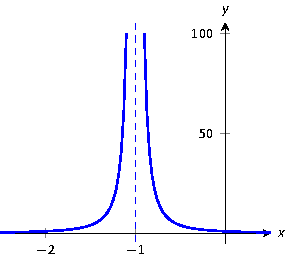
\includegraphics[scale=.8]{figures/fig01_06_ex_09}
}

\item
{$\ds f(x) = \frac{1}{(x-3)(x-5)^2}$.

\begin{minipage}[t]{.5\linewidth}
\begin{enumerate}
\item		$\ds \lim_{x\to 3^-} f(x)$
\item		$\ds \lim_{x\to 3^+} f(x)$
\item		$\ds \lim_{x\to 3} f(x)$
\end{enumerate}
\end{minipage}
\begin{minipage}[t]{.5\linewidth}
\begin{enumerate}\addtocounter{enumii}{3}
\item		$\ds \lim_{x\to 5^-} f(x)$
\item		$\ds \lim_{x\to 5^+} f(x)$
\item		$\ds \lim_{x\to 5} f(x)$
\end{enumerate}
\end{minipage}

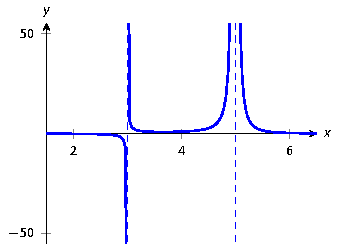
\includegraphics[scale=.8]{figures/fig01_06_ex_10}
}

\item
{$\ds f(x) = \frac{1}{e^x+1}$

\begin{minipage}[t]{.5\linewidth}
\begin{enumerate}
\item		$\ds \lim_{x\to -\infty} f(x)$
\item		$\ds \lim_{x\to \infty} f(x)$
\end{enumerate}
\end{minipage}
\begin{minipage}[t]{.5\linewidth}
\begin{enumerate}\addtocounter{enumii}{2}
\item		$\ds \lim_{x\to 0^-} f(x)$
\item		$\ds \lim_{x\to 0^+} f(x)$
\end{enumerate}
\end{minipage}

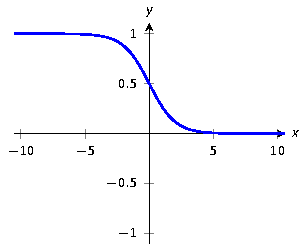
\includegraphics[scale=.8]{figures/fig01_06_ex_11}
}

\item
{$\ds f(x) = x^2\sin (\pi x)$

\begin{enumerate}
\item		$\ds \lim_{x\to -\infty} f(x)$
\item		$\ds \lim_{x\to \infty} f(x)$
\end{enumerate}

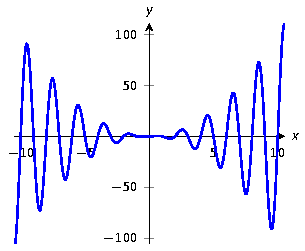
\includegraphics[scale=.8]{figures/fig01_06_ex_12}
}

\item
{$\ds f(x) = \cos (x)$

\begin{enumerate}
\item		$\ds \lim_{x\to -\infty} f(x)$
\item		$\ds \lim_{x\to \infty} f(x)$
\end{enumerate}

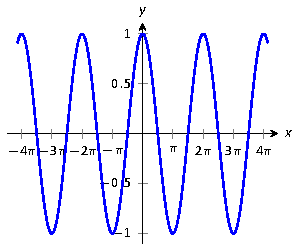
\includegraphics[scale=.8]{figures/fig01_06_ex_13}
}

\item
{$\ds f(x) = 2^x+10$
\begin{enumerate}
\item		$\ds \lim_{x\to -\infty} f(x)$
\item		$\ds \lim_{x\to \infty} f(x)$
\end{enumerate}

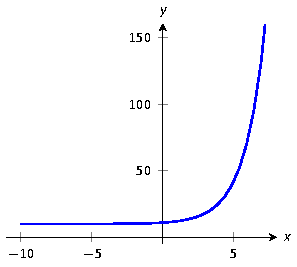
\includegraphics[scale=.8]{figures/fig01_06_ex_40}
}

\end{enumerate}

\vspace{.5cm}

%------------------------------------------
% END OF EXERCISES ON FIRST PAGE
%------------------------------------------
\end{multicols*}
\end{adjustwidth*}

\clearpage

\begin{adjustwidth*}{}{-2.25in}
\setlength{\columnsep}{25pt}
\begin{multicols*}{2}\small

In exercises 13--23, evaluate the limit.

\begin{multicols}{2}
\begin{enumerate}[1),start=13]
\item {$\ds \lim_{x \to -3^+} \frac{x-2}{x+3}$}
\item {$\ds \lim_{x \to 5^-} \frac{4}{x-5}$}
\item {$\ds \lim_{x \to 1} \frac{3-x}{(x-1)^2}$}
\item {$\ds \lim_{x \to \pi^-} \cot(x)$}
\item {$\ds \lim_{x\to\infty} \frac{x^3+2x^2+1}{5-x}$}
\item {$\ds \lim_{x\to-\infty} \frac{x^3+2x^2+1}{x^2-5}$}
\item {$\ds \lim_{x\to-\infty} \frac{x^3+2x^2+1}{5-x^2}$}
\item {$\ds \lim_{x \to \infty} \left( x - \sqrt{x} \right)$}
\item $\ds \lim_{x \to \infty} \frac{x+2}{\sqrt{9x^2 + 8}}$
\item $\ds \lim_{x \to -\infty} \frac{\sin^2(x)}{x^2}$
\item $\ds \lim_{x \to -\infty} \left( x^4 + x^5 \right)$
\end{enumerate}
\end{multicols}

\vspace{.5cm}

%---------------------------------------------
% END OF EXERCISES ON SECOND PAGE
%---------------------------------------------
\end{multicols*}
\end{adjustwidth*}
\afterexercises 

\cleardoublepage
\section{Continuity} \label{S:1.3.Continuity}

\begin{goals}
\item What does it mean to say that a function $f$ is continuous at $x = a$?  What role do limits play in determining whether or not a function is continuous at a point?
\item What properties do continuous functions have? 
\item How can we use continuous functions?
\end{goals}

%--------------------------------------
% SUBSECTION INTRODUCTION
%--------------------------------------
\subsection*{Introduction}

In Section~\ref{S:1.1.Limits}, we learned about how the concept of limits can be used to study the trend of a function near a fixed input value.  As we study such trends, we are fundamentally interested in knowing how well-behaved the function is at the given point, say $x = a$.  In this present section, we aim to expand our perspective and develop language and understanding to quantify how the function acts and how its value changes near a particular point.  Beyond thinking about whether or not the function has a limit $L$ at $x = a$, we will also consider the value of the function $f(a)$ and how this value is related to $\ds \lim_{x \to a} f(x)$.  Throughout,  we will build on and formalize ideas that we have encountered in several settings.

We begin to consider these issues through the following preview activity that asks you to consider the graph of a function with a variety of interesting behaviors.

\begin{marginfigure}[8cm]
\margingraphics{figures/1_7_PA1.eps}
\caption{The graph of $y = f(x)$.} \label{fig:1.3.PA1}
\end{marginfigure}

\begin{pa} \label{PA:1.3}
A function $f$ defined on $-4 < x < 4$ is given by the graph in Figure~\ref{fig:1.3.PA1}.  Use the graph to answer each of the following questions.  Note: to the right of $x = 2$, the graph of $f$ is exhibiting infinite oscillatory behavior similar to the function $\sin(\frac{\pi}{x})$ that we encountered in the key example early in Section~\ref{S:1.1.Limits}.

\ba
\item For each of the values $a = -3, -2, -1, 0, 1, 2, 3$, determine whether or not $\ds \lim_{x \to a} f(x)$ exists.  If the function has a limit $L$ at a given point, state the value of the limit using the notation $\ds \lim_{x \to a} f(x) = L$.  If the function does not have a limit at a given point, write a sentence to explain why.

\item For each of the values of $a$ from part (a) where $f$ has a limit, determine the value of $f(a)$ at each such point.  

\item For each of the values $a = -3, -2, -1, 0, 1, 2, 3$,  does $f(a)$ have the same value as $\ds \lim_{x \to a} f(x)$?
\ea
\end{pa} 

\afterpa

 % ACTIVITY 

%---------------------------------------
% SUBSECTION CONTINUITY
%---------------------------------------
\subsection*{Being continuous at a point} \index{continuous}

Intuitively, a function is continuous if we can draw it without ever lifting our pencil from the page.  Alternatively, we might say that the graph of a continuous function has no jumps or holes in it.  We first consider three specific situations in Figure~\ref{fig:1-3_Con} where all three functions have a limit at $a = 1$, and then work to make the idea of continuity more precise.

\begin{marginfigure} % MARGIN FIGURE
\captionsetup[subfigure]{labelformat=empty}
\subfloat{\margingraphics{figs/1/1-3_Cona.pdf}}

\subfloat{\margingraphics{figs/1/1-3_Conb.pdf}}

\subfloat{\margingraphics{figs/1/1-3_Conc.pdf}}
\caption{Functions $f$, $g$, and $h$ that demonstrate subtly different behaviors at $a = 1$.}
\label{fig:1-3_Con}
\end{marginfigure}

Note that  $f(1)$ is not defined, which leads to the resulting hole in the graph of $f$ at $a = 1$.  We will naturally say that $f$ is \emph{not continuous at $a = 1$}.  For the next function $g$ in in Figure~\ref{fig:1-3_Con}, we observe that while $\ds \lim_{x \to 1} g(x) = 3$, the value of $g(1) = 2$, and thus the limit does not equal the function value.  Here, too, we will say that $g$ is \emph{not continuous}, even though the function is defined at $a = 1$.  Finally, the function $h$ appears to be the most well-behaved of all three, since at $a = 1$ its limit and its function value agree.  That is,
\[ \lim_{x \to 1} h(x) = 3 = h(1). \]
With no hole or jump in the graph of $h$ at $a = 1$, we desire to say that $h$ is \emph{continuous} there.

More formally, we make the following definition.

\definition{Continuity}{ % DEFINITION
A function $f$ is \emph{continuous} \index{continuous at $x = a$} provided that
\begin{itemize}
\item $f$ has a limit as $x \to a$,
\item $f$ is defined at $x = a$, and
\item $\ds \lim_{x \to a} f(x) = f(a).$
\end{itemize}
A function $f$ is \emph{continuous} on an open interval I if $f$ is continuous at $c$ for all c in I. 

\begin{center}{\large {\bf Continuity at Endpoints}}\end{center}

A function $f$ is continuous at a left-endpoint, $a$, of a closed interval $[a,b]$, or {\em continuous from the right}, if
\[ \lim_{x \to a^+} f(x) = f(a), \]
and $f$ is continuous at a right-endpoint, $b$, of a closed interval $[a,b]$, or {\em continuous from the left}, if
\[ \lim_{x \to b^-} f(x) = f(b), \]
}% end definition

Conditions (a) and (b) are technically contained implicitly in (c), but we state them explicitly to emphasize their individual importance.  In words, (c) essentially says that a function is continuous at $x = a$ provided that its limit as $x \to a$ exists and equals its function value at $x = a$.  Thus, continuous functions are particularly nice:  to evaluate the limit of a continuous function at a point, all we need to do is evaluate the function.

\begin{example}\label{Ex:1.3.Eg1} %%Finding intervals of continuity 
Let $f$ be defined as shown in Figure~\ref{fig:1-3_Eg1}. Give the interval(s) on which $f$ is continuous.

\solution We proceed by examining the three criteria for continuity.
\begin{enumerate}[1)]
\item The limits $\ds \lim_{x \to a} f(x)$ exists for all $a$ between $0$ and $3$.
\item $f(a)$ is defined for all $a$ between $0$ and $3$, \textit{except for} $a=1$. We know immediately that $f$ cannot be continuous at $x=1$.
\item The limit $\ds \lim_{x \to a} f(x) = f(a)$ for all $a$ between $0$ and $3$, except, of course, for $a=1$. 
\item The function is defined at both $x = 0$ and $x = 3$, and both $\ds\lim_{x \to 0^+} f(x) = f(0)$ and $\ds\lim_{x \to 3^-} f(x) = f(3)$.
\end{enumerate}

Therefore, we conclude that $f$ is continuous at every point of $[0,3]$ except at $x=1$. Therefore $f$ is continuous on $[0,1)$ and $(1,3]$.
\end{example}

\begin{marginfigure}[-8cm]
\margingraphics{figs/1/figContinuous1.pdf}
\caption{A graph of $f$ in Example~\ref{Ex:1.3.Eg1}.}\label{fig:1-3_Eg1}
\end{marginfigure} % EXAMPLE 20 1.5 APEX

Let's now consider $p(x) = x^2 - 2x + 3$.  It can be proved that every polynomial is a continuous function at every real number, and thus if we would like to know                                                                                 $\lim_{x \to 2} p(x)$, we simply compute
$$\lim_{x \to 2} (x^2 - 2x + 3) = 2^2 - 2 \cdot 2 + 3 = 3.$$
This route of substituting an input value to evaluate a limit works anytime we know the function being considered is continuous.  Besides polynomial functions, all exponential functions and the sine and cosine functions are continuous at every point, as are many other familiar functions and combinations thereof.  

\begin{example}  % Determining intervals on which a function is continuous.
For each of the following functions, give the domain of the function and the interval(s) on which it is continuous.

\begin{enumerate}[1)]
\item $f(x) = 1/x$			
\item $f(x) = \sin(x)$
\item $f(x) = \sqrt{x}$
\item $f(x) = \sqrt{1-x^2}$
\item $f(x) = |x|$		
\end{enumerate}

\solution We examine each in turn.	
\begin{enumerate}[1)]
\item The domain of $f(x) = 1/x$ is $(-\infty,0) \cup (0,\infty)$. As it is a rational function, we apply the limit laws to recognize that $f$ is continuous on all of its domain.

\item The domain of $f(x) = \sin(x)$ is all real numbers, or $(-\infty,\infty)$. Applying the limit laws shows that $\sin x$ is continuous everywhere.

\item The domain of $f(x) = \sqrt{x}$ is $[0,\infty)$. Applying the limit laws shows that $f(x) = \sqrt{x}$ is continuous on its domain of $[0,\infty)$.

\item The domain of $f(x) = \sqrt{1-x^2}$ is $[-1,1]$. Applying the limit laws shows that $f$ is continuous on all of its domain, $[-1,1]$.

\item The domain of $f(x) = |x|$ is $(-\infty,\infty)$. We can define the absolute value function as $\ds f(x) = \left\{\begin{array}{cc} -x & x<0 \\ x & x\geq 0\end{array}\right.$. Each ``piece'' of this piece-wise defined function is continuous on all of its domain, giving that $f$ is continuous on $(-\infty,0)$ and $[0,\infty)$. As we saw before, we cannot assume this implies that $f$ is continuous on $(-\infty,\infty)$; we need to check that $\ds \lim_{x \to 0}f(x) = f(0)$, as $x=0$ is the point where $f$ transitions from one ``piece'' of its definition to the other. It is easy to verify that this is indeed true, hence we conclude that $f(x) = |x|$ is continuous everywhere.
\end{enumerate}
\end{example} % EXAMPLE 23 1.5 APEX

\begin{marginfigure}[6cm]
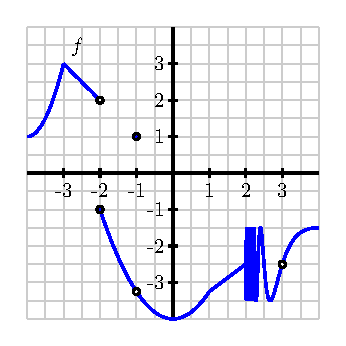
\includegraphics{figures/1_7_PA1.eps}
\caption{The graph of $y = f(x)$ for Activity~\ref{A:1.3.1}.} \label{fig:1-3_A1}
\end{marginfigure}

\begin{activity} \label{A:1.3.1}
This activity builds on your work in Preview Activity~\ref{PA:1.3}, using the same function $f$ as given by the graph that is repeated in Figure~\ref{fig:1-3_A1}.

\ba
	\item At which values of $a$ does $\ds \lim_{x \to a} f(x)$ not exist?
	\item At which values of $a$ is $f(a)$ not defined?
	\item At which values of $a$ does $f$ have a limit, but $\ds \lim_{x \to a} f(x) \ne f(a)$?
	\item State all values of $a$ for which $f$ is not continuous at $x = a$.
	\item Which condition is stronger, and hence implies the other:   $f$  has a limit at $x = a$ or  $f$ is continuous at $x = a$?  Explain, and hence complete the following sentence:  ``If $f$ \underline{\hspace{1.5in}} at $x = a$, then $f$ \underline{\hspace{1.5in}} at $x = a$,'' where you complete the blanks with \emph{has a limit} and \emph{is continuous}, using each phrase once.
\ea
\end{activity}
\begin{smallhint}
\ba
	\item Consider the left- and right-hand limits at each value.
	\item Carefully examine places on the graph where there's an open circle.
	\item Are there locations on the graph where the function has a limit but there's a hole in the graph?
	\item Remember that at least one of three conditions must fail: if the function lacks a limit, if the function is undefined, or if the limit exists but does not equal the function value, then $f$ is not continuous at the point.
	\item Note that the definition of being continuous requires the limit to exist.
\ea
\end{smallhint}
\begin{bighint}
\ba
	\item Consider the left- and right-hand limits at each value, and recall that they must both exist and be equal in order for the overall limit to exist.
	\item Carefully examine places on the graph where there's an open circle; at such locations, look vertically to see if the function has an assigned value at that point.
	\item Are there locations on the graph where the function has a limit but there's a hole in the graph?
	\item Remember that at least one of three conditions must fail: if the function lacks a limit, if the function is undefined, or if the limit exists but does not equal the function value, then $f$ is not continuous at the point.
	\item Note that the definition of being continuous requires the limit to exist.
\ea
\end{bighint}
\begin{activitySolution}
\ba
	\item $\lim_{x \to a} f(x)$ does not exist at $a = -2$ since $\lim_{x \to -2^-} f(x) = 2 \ne -1 = \lim_{x \to -2^+}$ and $\lim_{x \to a} f(x)$ does not exist at $a = +2$ since $\lim_{x \to 2^+} f(x)$ does not exist due to the infinitely oscillatory behavior of $f$.
	\item The only point at which $f$ is not defined is at $a = 3$.
	\item At $x = -1$, note that $\lim_{x \to -1} f(x)$ exists (and appears to have value approximately $-3.25$), but $f(-1) = 1$, and thus $\lim_{x \to -1} f(x) \ne f(-1)$.  At $x = 3$, $\lim_{x \to 3} f(x) = -2.5$, but $f(3)$ is not defined, so the limit exists but does not equal the function value.
	\item Based on our work in (a), (b), and (c), $f$ is not continuous at $a=-2$ and $a = 2$ because $f$ does not have a limit at those points; $f$ is not continuous at $a = 3$ since $f$ is not defined there; and $f$ is not continuous at $a = -1$ because at that point its limit does not equal its function value.
	\item ``If $f$ \underline{is continuous} at $x = a$, then $f$ \underline{has a limit} at $x = a$,'' since one of the defining properties of ``being continuous'' at $x = a$ is that the function has a limit at that input value.  This shows that being continuous is a stronger condition than having a limit.
\ea
\end{activitySolution}
\aftera % ACTIVITY 1.20 in AC 1.7

\begin{activity} \label{A:1.3.2}
State the interval(s) on which each of the following functions is continuous.
\bmtwo
\ba
\item $\ds f(x) = \sqrt{x-1} + \sqrt{5-x}$
\item $\ds f(x) = x\sin(x)$
\item $\ds f(x) = \tan(x)$
\item $\ds f(x) = \sqrt{\ln(x)}$
\ea
\emtwo
\end{activity}
\begin{smallhint}
\ba
	\item Consider the left- and right-hand limits at each value.
	\item Carefully examine places on the graph where there's an open circle.
	\item Are there locations on the graph where the function has a limit but there's a hole in the graph?
	\item Remember that at least one of three conditions must fail: if the function lacks a limit, if the function is undefined, or if the limit exists but does not equal the function value, then $f$ is not continuous at the point.
	\item Note that the definition of being continuous requires the limit to exist.
\ea
\end{smallhint}
\begin{bighint}
\ba
	\item Consider the left- and right-hand limits at each value, and recall that they must both exist and be equal in order for the overall limit to exist.
	\item Carefully examine places on the graph where there's an open circle; at such locations, look vertically to see if the function has an assigned value at that point.
	\item Are there locations on the graph where the function has a limit but there's a hole in the graph?
	\item Remember that at least one of three conditions must fail: if the function lacks a limit, if the function is undefined, or if the limit exists but does not equal the function value, then $f$ is not continuous at the point.
	\item Note that the definition of being continuous requires the limit to exist.
\ea
\end{bighint}
\begin{activitySolution}
\ba
	\item $\lim_{x \to a} f(x)$ does not exist at $a = -2$ since $\lim_{x \to -2^-} f(x) = 2 \ne -1 = \lim_{x \to -2^+}$ and $\lim_{x \to a} f(x)$ does not exist at $a = +2$ since $\lim_{x \to 2^+} f(x)$ does not exist due to the infinitely oscillatory behavior of $f$.
	\item The only point at which $f$ is not defined is at $a = 3$.
	\item At $x = -1$, note that $\lim_{x \to -1} f(x)$ exists (and appears to have value approximately $-3.25$), but $f(-1) = 1$, and thus $\lim_{x \to -1} f(x) \ne f(-1)$.  At $x = 3$, $\lim_{x \to 3} f(x) = -2.5$, but $f(3)$ is not defined, so the limit exists but does not equal the function value.
	\item Based on our work in (a), (b), and (c), $f$ is not continuous at $a=-2$ and $a = 2$ because $f$ does not have a limit at those points; $f$ is not continuous at $a = 3$ since $f$ is not defined there; and $f$ is not continuous at $a = -1$ because at that point its limit does not equal its function value.
	\item ``If $f$ \underline{is continuous} at $x = a$, then $f$ \underline{has a limit} at $x = a$,'' since one of the defining properties of ``being continuous'' at $x = a$ is that the function has a limit at that input value.  This shows that being continuous is a stronger condition than having a limit.
\ea
\end{activitySolution}
\aftera % ACTIVITY 

%----------------------------------------------------------
% SUBSECTION INTERMEDIATE VALUE THEOREM
%----------------------------------------------------------
\subsection*{Intermediate Value Theorem}

This intuitive notion of continuity does help us understand another important concept as follows. Suppose $f$ is defined on $[1,2]$ and $f(1) = -10$ and $f(2) = 5$. If $f$ is continuous on $[1,2]$ (i.e., its graph can be sketched as a continuous line from $(1,-10)$ to $(2,5)$) then we know intuitively that somewhere on $[1,2]$ $f$ must be equal to $-9$, and $-8$, and $-7,\ -6,\ \ldots,\ 0,\ 1/2,$ etc. In short, $f$ takes on all \textit{intermediate} values between $-10$ and $5$. It may take on more values; $f$ may actually equal 6 at some time, for instance, but we are guaranteed all values between $-10$ and $5$. 

While this notion seems intuitive, it is not trivial to prove and its importance is profound. Therefore the concept is stated in the form of a theorem.

\concept{Intermediate Value Theorem}{% CONCEPT
Let $f$ be a continuous function on $[a,b]$ and, without loss of generality, let $f(a) < f(b)$. Then for every value $y$, where $f(a) < y < f(b)$, there is a value $c$ in $[a,b]$ such that $f(c) = y$. 
}% end concept

One important application of the Intermediate Value Theorem is root finding. Given a function $f$, we are often interested in finding values of $x$ where $f(x) = 0$. These roots may be very difficult to find exactly. Good approximations can be found through successive applications of this theorem. Suppose through direct computation we find that $f(a) <0 $ and $f(b)>0$, where $a<b$. The Intermediate Value Theorem states that there is a $c$ in $[a,b]$ such that $f(c) = 0$. The theorem does not give us any clue as to where that value is in the interval $[a,b]$, just that it exists. 

There is a technique that produces a good approximation of $c$. Let $d$ be the midpoint of the interval $[a,b]$ and consider $f(d)$. There are three possibilities:
\begin{enumerate}[1)]
\item $f(d) = 0$ -- we got lucky and stumbled on the actual value. We stop as we found a root.
\item $f(d) <0$ Then we know there is a root of $f$ on the interval $[d,b]$ -- we have halved the size of our interval, hence are closer to a good approximation of the root.
\item $f(d) >0$ Then we know there is a root of $f$ on the interval $[a,d]$ -- again,we have halved the size of our interval, hence are closer to a good approximation of the root.
\end{enumerate}
	
Successively applying this technique is called the \emph{Bisection Method} \index{Bisection Method} of root finding. We continue until the interval is sufficiently small. We demonstrate this in the following example.

\begin{marginfigure}[6cm]
\margingraphics{figs/1/figXMinusCosX.pdf} 
\caption{Graphing a root of $f(x) = x-\cos(x)$.}\label{fig:1-3_Eg3}
\end{marginfigure}

\begin{margintable}
\scalebox{1.1}{
\begin{tabular}{ccc}
Iteration \# & Interval & Midpoint Sign \\ \hline
			1 & $[0.7,0.9]$ & $f(0.8) >0$ \\
			2 & $[0.7,0.8] $ & $f(0.75) >0$ \\
			3 & $[0.7,0.75]$ & $f(0.725)<0$\\
			4 & $[0.725,0.75]$ & $f(0.7375)<0$\\
			5 & $[0.7375,0.75]$ & $f(0.7438)>0$\\
			6 & $[0.7375,0.7438]$ & $f(0.7407)>0$\\
			7 & $[0.7375,0.7407]$ & $f(0.7391)>0$\\
			8 & $[0.7375,0.7391]$ & $f(0.7383)<0$\\
			9 & $[0.7383,0.7391]$ & $f(0.7387)<0$\\
			10 & $[0.7387,0.7391]$ & $f(0.7389)<0$\\
			11 & $[0.7389,0.7391]$ & $f(0.7390)<0$\\
			12 & $[0.7390,0.7391]$ &   \\
\end{tabular}
} % end scalebox 
\caption{Iterations of the Bisection Method of Root Finding}\label{T:1-3_Eg3}
\end{margintable}

\begin{example}   %Using the Bisection Method 
Approximate the root of $f(x) = x-\cos x$, accurate to three places after the decimal.

\solution Consider the graph of $f(x) = x-\cos x$, shown in Figure~\ref{fig:1-3_Eg3}. It is clear that the graph crosses the $x$-axis somewhere near $x=0.8$. To start the Bisection Method, pick an interval that contains $0.8$. We choose $[0.7,0.9]$. Note that all we care about are signs of $f(x)$, not their actual value, so this is all we display.

\begin{description}
\item[Iteration 1:] $f(0.7) < 0$, $f(0.9) > 0$, and $f(0.8) >0$. So replace $0.9$ with $0.8$ and repeat.
\item[Iteration 2:] $f(0.7)<0$, $f(0.8) > 0$, and at the midpoint, $0.75$, we have $f(0.75) >0 $. So replace $0.8$ with $0.75$ and repeat. Note that we don't need to continue to check the endpoints, just the midpoint. Thus we put the rest of the iterations in Table~\ref{T:1-3_Eg3}.
\end{description}

Notice that in the $12^{\text{th}}$ iteration we have the endpoints of the interval each starting with $0.739$. Thus we have narrowed the zero down to an accuracy of the first three places after the decimal. Using a computer, we have 
\[ f(0.7390) = -0.00014, \quad f(0.7391) = 0.000024. \] 
Either endpoint of the interval gives a good approximation of where $f$ is $0$. The Intermediate Value Theorem states that the actual zero is still within this interval. While we do not know its exact value, we know it starts with $0.739$. 

This type of exercise is rarely done by hand. Rather, it is simple to program a computer to run such an algorithm and stop when the endpoints differ by a preset small amount. One of the authors did write such a program and found the zero of $f$, accurate to $10$ places after the decimal, to be $0.7390851332$. While it took a few minutes to write the program, it took less than a thousandth of a second for the program to run the necessary $35$ iterations. In less than $8$ hundredths of a second, the zero was calculated to $100$ decimal places (with less than $200$ iterations).
\end{example}
 % EXAMPLE

It is a simple matter to extend the Bisection Method to solve similar problems to $f(x) = 0$. For instance, we can solve $f(x) = 1$. This may seem obvious, but to many it is not. It actually works very well to define a new function $g$ where $g(x) = f(x) - 1$. Then use the Bisection Method to solve $g(x)=0$.  

Similarly, given two functions $f$ and $g$, we can use the Bisection Method to solve $f(x) = g(x)$. Once again, create a new function $h$ where $h(x) = f(x)-g(x)$ and solve $h(x) = 0$. 

\begin{activity} \label{A:1.3.3}
Use the Bisection Method to approximate, accurate to two decimal places, the value of the root of the given functions and intervals.

\ba
\item $\ds f(x) = x^2 + 2x - 4; \quad [1,1.5]$
\item $\ds f(x) = e^x - 2; \quad [0.65, 0.7]$
\ea
\end{activity}

\aftera % ACTIVITY 

%--------------
% SUMMARY
%--------------
\begin{summary}
%\item A function $f$ has limit $L$ as $x \to a$ if and only if $f$ has a left-hand limit at $x = a$, has a right-hand limit at $x = a$, and the left- and right-hand limits are equal.  Visually, this means that there can be a hole in the graph at $x = a$, but the function must approach the same single value from either side of $x = a$.
\item A function $f$ is continuous at $x = a$ whenever $f(a)$ is defined, $f$ has a limit as $x \to a$, and the value of the limit and the value of the function agree.  This guarantees that there is not a hole or jump in the graph of $f$ at $x = a$.

\item We can use the Intermediate Value Theorem to determine if there may be a root of a continuous function on a closed interval.
%\item A function $f$ is differentiable at $x = a$ whenever $f'(a)$ exists, which means that $f$ has a tangent line at $(a,f(a))$ and thus $f$ is locally linear at the value $x = a$.  Informally, this means that the function looks like a line when viewed up close at $(a,f(a))$ and that there is not a corner point or cusp at $(a,f(a))$. 
%\item Of the three conditions discussed in this section (having a limit at $x = a$, being continuous at $x = a$, and being differentiable at $x = a$), the strongest condition is being differentiable, and the next strongest is being continuous.  In particular, if $f$ is differentiable at $x = a$, then $f$ is also continuous at $x = a$, and if $f$ is continuous at $x = a$, then $f$ has a limit at $x = a$.
\end{summary}

\clearpage

%--------------
% EXERCISES
%--------------
\begin{adjustwidth*}{}{-2.25in}
\textbf{{\large Exercises}}
\setlength{\columnsep}{25pt}
\begin{multicols*}{2}
\noindent Terms and Concepts \small

\begin{enumerate}[1)]
\item {In your own words, describe what it means for a function to be continuous.}
\item {In your own words, describe what the Intermediate Value Theorem states.}
\item {What is a ``root'' of a function?}
\item {Given functions $f$ and $g$ on an interval $I$, how can the Bisection Method be used to find a value $c$ where $f(c) = g(c)$?}
\item {T/F:	If $f$ is defined on an open interval containing $c$, and $\ds \lim_{x\to c}f(x)$ exists, then $f$ is continuous at $c$.}
\item {T/F: If $f$ is continuous at $c$, then $\ds \lim_{x\to c}f(x)$ exists.}
\item {T/F: If $f$ is continuous at $c$, then $\ds \lim_{x\to c^+}f(x) = f(c)$.}
\item {T/F: If $f$ is continuous on $[a,b]$, then $\ds\lim_{x\to a^-}f(x) = f(a)$.}
\item {T/F: If $f$ is continuous on $[0,1)$ and $[1,2)$, then $f$ is continuous on $[0,2)$.}
\item {T/F: The sum of continuous functions is also continuous.}
\end{enumerate} 

\noindent {\normalsize Problems\\} \small

\noindent In exercises 11--17, a graph of $f$ is given along with a value $a$.  Determine if $f$ is continuous at $a$; if it is not, state why it is not.

\begin{enumerate}[1),resume]
\item
{\noindent $a = 1$

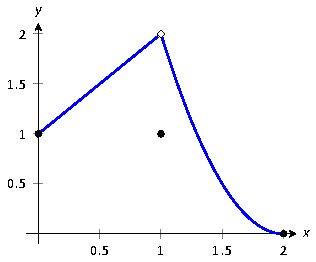
\includegraphics[scale=.8]{figures/fig01_04_ex_05}
}

\item
{\noindent $a = 1$

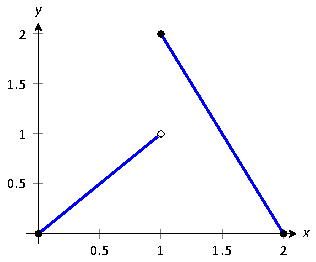
\includegraphics[scale=.8]{figures/fig01_04_ex_06}
}

\vspace{.5cm}

\item
{\noindent $a = 1$

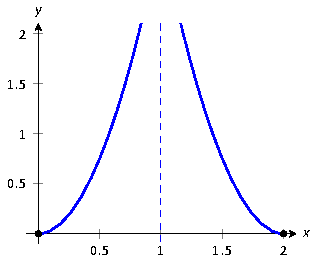
\includegraphics[scale=.8]{figures/fig01_04_ex_07}
}

\item
{\noindent $a = 0$

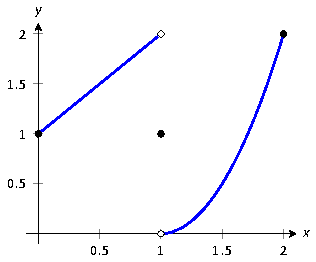
\includegraphics[scale=.8]{figures/fig01_04_ex_08}
}

\item
{\noindent $a = 1$

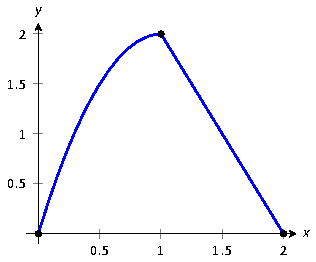
\includegraphics[scale=.8]{figures/fig01_04_ex_09}
}

\item
{\noindent $a = 4$

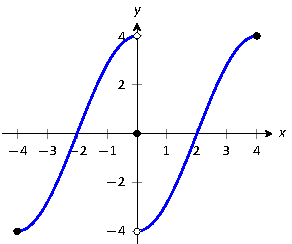
\includegraphics[scale=.8]{figures/fig01_04_ex_10}
}

\item
{\begin{enumerate}
\item		$a = -2$
\item		$a=0$
\item		$a=2$
\end{enumerate}

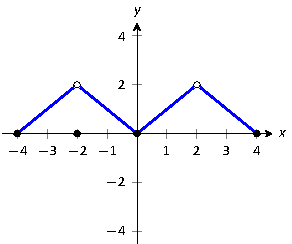
\includegraphics[scale=.8]{figures/fig01_04_ex_11}
}

\end{enumerate}

\vspace{.5cm}

%------------------------------------------
% END OF EXERCISES ON FIRST PAGE
%------------------------------------------
\end{multicols*}
\end{adjustwidth*}

\clearpage

\begin{adjustwidth*}{}{-2.25in}
\setlength{\columnsep}{25pt}
\begin{multicols*}{2}\small

In exercises 18--21, determine if $f$ is continuous at the indicated values.  If not, explain why.

\begin{enumerate}[1),start=18]
\item 
{$\ds f(x) = \left\{\begin{array}{ccc} 
1		& & x=0\\
\ds\frac{\sin(x)}{x} & & x>0
\end{array}\right.
$
\begin{enumerate}
\item		$x=0$
\item		$x=\pi$
\end{enumerate}
}

\item 
{$\ds f(x) = \left\{\begin{array}{ccc} 
x^3-x		& & x<1\\
x-2 & & x\geq 1
\end{array}\right.
$
\begin{enumerate}
\item		$x=0$
\item		$x=1$
\end{enumerate}
}

\item 
{$\ds f(x) = \left\{\begin{array}{ccc} 
\ds\frac{x^2+5x+4}{x^2+3x+2}		& &  x\neq -1\\
3 & & x=-1
\end{array}\right.
$
\begin{enumerate}
\item		$x=-1$
\item		$x=10$
\end{enumerate}
}

\item
{$\ds f(x) = \left\{\begin{array}{ccc}
\ds\frac{x^2-64}{x^2-11 x+24}		& &  x\neq 8\\
5 & & x=8
\end{array}\right.
$
\begin{enumerate}
\item		$x=0$
\item		$x=8$
\end{enumerate}
}
\end{enumerate}

\vspace{.5cm}

\noindent In exercises 22--32, give the intervals on which the given function is continuous.

\begin{enumerate}[1),start=22]
\item $\ds f(x) = x^2-3x+9$
\item $\ds g(x) = \sqrt{x^2-4}$
\item $\ds h(k) = \sqrt{1-k}+\sqrt{k+1}$
\item $\ds f(t) = \sqrt{5t^2-30}$
\item $\ds g(t) = \frac{1}{\sqrt{1-t^2}}$
\item $\ds g(x) = \frac{1}{1+x^2}$
\item $\ds f(x) = e^x$
\item $\ds g(s) = \ln s$
\item $\ds h(t) = \cos(t)$
\item $\ds f(k) = \sqrt{1-e^k}$
\item $\ds f(x) = \sin(e^x+x^2)$
\end{enumerate}

\vspace{.5cm}

\noindent In exercises 33--34, use the Bisection Method to approximate, accurate to two decimal places, the value of the root of the given function in the given interval.

\begin{enumerate}[1),start=33]
\item $\ds f(x) = \sin(x) - \frac{1}{2}; \quad [0.5, 0.55]$
\item $\ds f(x) = \cos(x) - \sin(x); \quad [0.7, 0.8]$
\end{enumerate}

%---------------------------------------------
% END OF EXERCISES ON SECOND PAGE
%---------------------------------------------
\end{multicols*}
\end{adjustwidth*}
\afterexercises 

\cleardoublepage
\section{Epsilon-Delta Definition of a Limit} \label{S:1.4.precise}

\begin{goals}
\item What do we mean by saying "arbitrarily close"?
\item What is the precise definition of a \emph{limit}?
\item What are $\epsilon$ and $\delta$ and how do they help in determining the value of the limit of a function at a point?
\end{goals}

%-----------------------------------
% SUBSECTION INTRODUCTION
%-----------------------------------
\subsection*{Introduction}

Recall our definition of a limit of a function from Section~\ref{S:1.1.Limits}.

\definition{The Limit of a Function}{ %DEFINITION 
Given a function $f$, a fixed input $x = a$, and a real number $L$, we say that \emph{$f$ has limit\index{limit!definition} $L$ as $x$ approaches $a$}, and write
\[ \lim_{x \to a} f(x) = L \]
provided that we can make $f(x)$ as close to $L$ as we like by taking $x$ sufficiently close (but not equal) to $a$.  If we cannot make $f(x)$ as close to a single value as we would like as $x$ approaches $a$, then we say that \emph{$f$ does not have a limit as $x$ approaches $a$.}
} % end definition

The problem with this definition is that the words "approaches" and "close" are not exact.  In what way does the variable $x$ approach $a$? How "close" do $x$ and $y$ have to be to $a$ and $L$, respectively? Finally, what determines "sufficiently close"? The precise definition we describe in this section comes from formalizing our original definition.  A quick restatement gets us closer to what we want:

\begin{description}
\item ``If $x$ is within a certain \textit{tolerance level} of $a$, then the corresponding value $y=f(x)$ is within a certain \textit{tolerance level} of $L$.''
\end{description}

The accepted notation for the $x$-tolerance is the lowercase Greek letter delta, or $\delta$, and the $y$-tolerance is lowercase epsilon, or $\epsilon$. One more rephrasing nearly gets us to the actual definition:

\begin{description}
\item ``If $x$ is within $\delta$ units of $a$, then the corresponding value of $y$ is within $\epsilon$ units of $L$.''
\end{description}

Note that this means (let the "$\longrightarrow$" represent the word "implies"):
$\ds a - \delta < x < a + \delta \longrightarrow L - \epsilon < y < L + \epsilon$ or  $\ds |x - a| < \delta \longrightarrow  |y - L| < \epsilon$. The point is that $\delta$ and $\epsilon$, being tolerances, can be any positive (but typically small) values.  Finally, we have the formal definition of the limit with the notation  seen in the previous section.

\definition{The Limit of a Function $f$} %DEFINITION 
{Let $f$ be a function defined on an open interval containing $a$. The notation $$\displaystyle \lim_{x\rightarrow a} f(x) = L,$$ read as ``the limit of $f(x)$, as $x$ approaches $a$, is $L$,'' 
means that given any $\epsilon > 0$, there exists $\delta > 0$ such that 
whenever $|x - a| < \delta$, we have $|f(x) - L| < \epsilon$.\index{limit!definition}
}% end definition

Mathematicians often enjoy writing ideas without using any words. Here is the wordless definition of the limit:
{\small \[ \ds \lim_{x \to a} f(x) = L \iff \forall \ \epsilon > 0, \exists \ \delta > 0 \ \mbox{s.t.} \ |x - a| < \delta \longrightarrow |f(x) - L| < \epsilon. \]}
There is an emphasis here that we may have passed over before.  In the definition, the $y$-tolerance $\epsilon$ is given \textit{first} and then the limit will exist {\em if} we can find an $x$-tolerance $\delta$ that works.  

It is time for an example.  Note that the explanation is long, but it will take you through all steps necessary to understand the ideas.

%\ifthenelse{\boolean{longpage}}%
%{\mtable{.4}{Illustrating the $\epsilon-\delta$ process.}{fig:choose_e_d}{%
		%\begin{tabular}{cc} 
		%\myincludegraphics{figures/figLimitProof1a}&
		%\myincludegraphics{figures/figLimitProof1b}
		%\end{tabular}
		%\vskip \baselineskip
		%\parbox{200pt}{\centering With $\epsilon=0.5$, we pick any $\delta < 1.75$.}
		%}
%}
%\mtable{.45}{Illustrating the $\epsilon-\delta$ process.}{fig:choose_e_d}{%
%		\begin{tabular}{c} 
%		\myincludegraphics{figures/figLimitProof1a}\\
%		\myincludegraphics{figures/figLimitProof1b}\\
%		\noindent\parbox{200pt}{With $\epsilon=0.5$, we pick any $\delta < 1.75$.}
%		\end{tabular}
%	}

\begin{marginfigure}[7cm] % MARGIN FIGURE
\captionsetup[subfigure]{labelformat=empty}
\subfloat{\margingraphics{figures/figLimitProof1a}}

\subfloat{\margingraphics{figures/figLimitProof1b}}
\caption{Illustrating the $\epsilon-\delta$ process. With $\epsilon=0.5$, we pick any $\delta < 1.75$.}
\label{fig:1-4_Eg1}
\end{marginfigure}

\begin{example} \label{Ex:1.4.Eg1}
Show that $\ds \lim_{x \to 4} \sqrt{x} = 2 $.

\solution Before we use the formal definition, let's try some numerical tolerances.  What if the $y$ tolerance is $0.5$, or $\epsilon =0.5$?  How close to $4$ does $x$ have to be so that $y$ is within $0.5$ units of $2$ (or $1.5 < y < 2.5$)?  In this case, we can just square these values since $y = \sqrt{x}$ to get
$1.5^2 < x < 2.5^2,$ or 
\[ 2.25 < x < 6.25.\]
So, what is the desired $x$ tolerance?  Remember, we want to find a symmetric interval of $x$ values, namely
$4 - \delta < x < 4 + \delta$.  The lower bound of $2.25$ is $1.75$ units from $4$; the upper bound of $6.25$ is $2.25$ units from $4$. We need the smaller of these two distances; we must have $\delta = 1.75$. See Figure~\ref{fig:1-4_Eg1}.

Now read it in the correct way:  For the $y$ tolerance $\epsilon =0.5$, we have found an $x$ tolerance, $\delta = 1.75$, so that whenever $x$ is within $\delta$ units of $4$, then $y$ is within $\epsilon$ units of $2$.  That's what we were trying to find.
  
Let's try another value of $\epsilon$.  What if the $y$ tolerance is $0.01$, or $\epsilon =0.01$?  How close to $4$ does $x$ have to be in order for $y$ to be within $0.01$ units of $2$ (or $1.99 < y < 2.01$)?  Again, we just square these values to get $1.99^2 < x < 2.01^2$, or 
\[ 3.9601 < x < 4.0401.\]  
So, what is the desired $x$ tolerance?  In this case we must have $\delta = 0.0399$.  Note that in some sense, it looks like there are two tolerances (below $4$ of $0.0399$ units and above $4$ of $0.0401$ units).  However, we couldn't use the larger value of $0.0401$ for $\delta$ since then the interval for $x$ would be  $3.9599 < x < 4.0401$ resulting in $y$ values of $1.98995 < y < 2.01$ (which contains values NOT within $0.01$ units of $2$).

What we have so far: if $\epsilon =0.5$, then $\delta = 1.75$ and if $\epsilon =0.01$, then $\delta = 0.0399$. A pattern is not easy to see, so we switch to general $\epsilon$ and $\delta$ and do the calculations symbolically.  We start by assuming $y=\sqrt{x}$ is within $\epsilon$ units of $2$:
\begin{eqnarray*}
|y - 2| < \epsilon &\\
-\epsilon < y - 2 < \epsilon& \qquad \textrm{(Absolute value)}\\
-\epsilon < \sqrt{x} - 2 < \epsilon  &\qquad (y=\sqrt{x})\\
2 - \epsilon < \sqrt{x} < 2+ \epsilon &\qquad \textrm{ (Add 2)}\\
(2 - \epsilon)^2 < x < (2+ \epsilon) ^2 &\qquad \textrm{ (Square all)}\\
4 - 4\epsilon + \epsilon^2 < x < 4 + 4\epsilon + \epsilon^2 &\qquad \textrm{ (Expand)}\\
4 - (4\epsilon - \epsilon^2) < x < 4 + (4\epsilon + \epsilon^2) &\qquad \textrm{ (Rewrite)}
\end{eqnarray*}

Since we want this last interval to describe an $x$ tolerance around $4$, we have that either $\delta = 4\epsilon + \epsilon^2$ or $\delta = 4\epsilon - \epsilon^2$. However, as we saw in the case when $\epsilon = 0.01$, we want the smaller of the two values for $\delta$.  So, to conclude this part, we set
$\delta$ equal to the minimum of these two values, or $\delta = \min\{4\epsilon + \epsilon^2, 4\epsilon - \epsilon^2\}$.  Since $\epsilon > 0$, the minimum will occur when $\delta = 4\epsilon - \epsilon^2$.  That's the formula!  

We can check this for our previous values.  If $\epsilon=0.5$, the formula gives
$\delta = 4(0.5) - (0.5)^2 = 1.75$ and when $\epsilon=0.01$, the formula gives $\delta = 4(0.01) - (0.01)^2 = 0.399$.

So given any $\epsilon >0$, we can set $\delta = 4\epsilon - \epsilon^2$ and the limit definition is satisfied.  We have shown formally (and finally!) that $\displaystyle \lim_{x\rightarrow 4} \sqrt{x} = 2 $.
\end{example}

%FOOTNOTE $**$: Actually, it is a pain, but this won't work if $\epsilon \ge 4$.  This shouldn't really occur since $\epsilon$ is supposed to be small, but it could happen.  In the cases where $\epsilon \ge 4$, just take $\delta = 1$ and you'll be fine. %EXAMPLE
 
If you are thinking this process is long, you would be right.  The previous example is also a bit unsatisfying in that $\sqrt{4}=2$; why work so hard to prove something so obvious? Many $\epsilon-\delta$ proofs are long and difficult to do. In this section, we will focus on examples where the answer is, frankly, obvious, because the non--obvious examples are even harder.  That is why theorems about limits are so useful! After doing a few more $\epsilon$--$\delta$ proofs, you will really appreciate the analytical "short cuts" we previously discussed. 

\begin{example} \label{Ex:1.4.Eg2} 
Show that $\ds \lim_{x \to 2} x^2 = 4$.

\solution Let's do this example symbolically from the start.  Let $\epsilon > 0$ be given; we want $|y-4| < \epsilon$, i.e.,  $|x^2-4| < \epsilon$.  How do we find $\delta$ such that when $|x-2| < \delta$, we are guaranteed that $|x^2-4|<\epsilon$?% for some $\delta$ (in terms of $\epsilon$)?

This is a bit trickier than the previous example, but let's start by noticing that 
$|x^2-4| = |x-2|\cdot|x+2|$.  Consider:
\begin{equation} |x^2-4| < \epsilon \longrightarrow |x-2|\cdot|x+2| < \epsilon \longrightarrow |x-2| < \frac{\epsilon}{|x+2|}.
\label{eq:limit1}
\end{equation} 
Could we not set $\ds \delta = \frac{\epsilon}{|x+2|}$?  

We are close to an answer, but the catch is that $\delta$ must be a \textit{constant} value (so it can't contain $x$).  There is a way to work around this, but we do have to make an assumption.  Remember that $\epsilon$ is supposed to be a small number, which implies that $\delta$ will also be a small value.  In particular, we can (probably) assume that $\delta < 1$.  If this is true, then $|x-2| < \delta$ would imply that $|x-2| < 1$, giving $1 < x < 3$.  

Now, back to the fraction $\ds \frac{\epsilon}{|x+2|}$.  If $1<x<3$, then $3<x+2<5$.  Taking reciprocals, we have $\ds \frac{1}{5}<\frac{1}{|x+2|}<\frac{1}{3}$ so that, in particular, 
\begin{equation} \frac{\epsilon}{5}<\frac{\epsilon}{|x+2|}.
\label{eq:limit2}
\end{equation}  
This suggests that we set 
$\ds \delta = \frac{\epsilon}{5}$. To see why, let's go back to the equations:

\begin{eqnarray*}
|x - 2| &<& \delta \\
|x - 2| &<& \frac{\epsilon}{5} \\%\qquad \text{\small(Our choice of $\delta$)}\\
|x - 2|\cdot|x + 2| &<& |x + 2|\cdot\frac{\epsilon}{5} \\%\qquad \text{\small(Multiply by $|x+2|$)}\\
|x^2 - 4|&<& |x + 2|\cdot\frac{\epsilon}{5} \\%\qquad \text{\small(Combine left side)}\\
|x^2 - 4|&<& |x + 2|\cdot\frac{\epsilon}{5} <|x + 2|\cdot\frac{\epsilon}{|x+2|}=\epsilon  %\qquad \text{\small(Using (\ref{eq:limit2}) as long as $\delta <1$)}
\end{eqnarray*}

We have arrived at $|x^2 - 4|<\epsilon$ as desired.  Note again, in order to make this happen we needed $\delta$ to first be less than 1.  That is a safe assumption; we want $\epsilon$ to be arbitrarily small, forcing $\delta$ to also be small. 

We have also picked $\delta$ to be smaller than ``necessary.'' We could get by with a slightly larger $\delta$, as shown in Figure~\ref{fig:1-4_Eg2}. The dashed, red lines show the boundaries defined by our choice of $\epsilon$. The gray, dashed lines show the boundaries defined by setting $\delta = \epsilon/5$. Note how these gray lines are within the red lines. That is perfectly fine; by choosing $x$ within the gray lines we are guaranteed that $f(x)$ will be within $\epsilon$ of $4$.%If the value we eventually used for $\delta$, namely $\epsilon/5$, is not less than 1, this proof won't work.  For the final fix, we instead set $\delta$ to be the minimum of 1 and $\epsilon/5$. This way all calculations above work.  

In summary, given $\epsilon > 0$, set $\delta=\epsilon/5$.  Then $|x - 2| < \delta$ implies 
$|x^2 - 4|< \epsilon$ (i.e. $|y - 4|< \epsilon$) as desired.  We have shown that $\ds \lim_{x\rightarrow 2} x^2 = 4 $. Figure~\ref{fig:1-4_Eg2} gives a visualization of this; by restricting $x$ to values within $\delta = \epsilon/5$ of $2$, we see that $f(x)$ is within $\epsilon$ of $4$.
\end{example}

\begin{marginfigure}[-8cm]
%\margingraphics{figures/figLimitProof2a}
\margingraphics{figs/1/1-4_Eg2.pdf}
\caption{Choosing $\delta = \epsilon/5$ in Example \ref{Ex:1.4.Eg2}.}\label{fig:1-4_Eg2}
\end{marginfigure} %EXAMPLE

\begin{example} \label{Ex:1.4.Eg3}
Show that $\ds \lim_{x \to 0} e^x = 1 $.

\solution Symbolically, we want to take the equation $|e^x - 1| < \epsilon$ and unravel it to the form $|x-0| < \delta$.  Let's look at some calculations:
\begin{eqnarray*}
|e^x - 1| < \epsilon&\\
-\epsilon < e^x - 1 < \epsilon& \qquad \textrm{(Definition of absolute value)}\\
1-\epsilon < e^x < 1+\epsilon & \qquad \textrm{(Add 1)}\\
\ln(1-\epsilon) < x < \ln(1+\epsilon) & \qquad \textrm{(Take natural logs)}
\end{eqnarray*}
Making the safe assumption that $\epsilon<1$ ensures the last inequality is valid (i.e., so that $\ln (1-\epsilon)$ is defined). Recall $\ln(1)= 0$ and $\ln(x)<0$ when $0<x<1$. So $\ln (1-\epsilon) <0$, hence we consider its absolute value. We can then set $\delta$ to be the minimum of $|\ln(1-\epsilon)|$ and $\ln(1+\epsilon)$; i.e.,  
%  Well, there is a catch.  The value of $\epsilon$ is supposed to be small, but if it happens that $\epsilon \ge 1$, then $\ln(1-\epsilon)$ would be undefined!  The way to work around this is to simply define a new epsilon that is guaranteed to be smaller than the original epsilon \textit{and} less than 1 (let's say less than 1/2 just to be on the safe side).  Let's call this new value $\epsilon_1$ and define it to be $\epsilon_1 = \min\{\epsilon, 1/2\}$.  Then we can use the calculations above to define 
\[ \delta = \min\{|\ln(1-\epsilon)|, \ln(1+\epsilon)\}. \]


Now, we work through the actual the proof:

\begin{eqnarray*}
|x - 0|<\delta\\
-\delta < x < \delta& \qquad \textrm{(Definition of absolute value)}\\
\ln(1-\epsilon) < x < \ln(1+\epsilon) & \qquad \textrm{(By our choice of}\; \delta)\\
1-\epsilon < e^x < 1+\epsilon & \qquad \textrm{(Exponentiate)}\\
-\epsilon < e^x - 1 < \epsilon & \qquad \textrm{(Subtract 1)}\\
%-\epsilon < e^x - 1 < \epsilon & \qquad \textrm{(Since}\; \epsilon_1 \le \epsilon)\\
\end{eqnarray*}

In summary, given $\epsilon > 0$, let $\delta = \min\{|\ln(1-\epsilon |, \ln(1+\epsilon)\}$. Then $|x - 0| < \delta$ implies $|e^x - 1|< \epsilon$ as desired.  We have shown that $\displaystyle \lim_{x\rightarrow 0} e^x = 1 $.
\end{example} %EXAMPLE

We note that we could actually show that $\ds \lim_{x \to a} e^x = e^a$ for any constant $a$.  We do this by factoring out $e^a$ from both sides, leaving us to show $\ds \lim_{x \to a} e^{x-a} = 1$ instead.  By using the substitution $y=x-a$, this reduces to showing $\lim_{y \to 0} e^y = 1 $ which we just did in the last example.  As an added benefit, this shows that in fact the function $f(x)=e^x$ is \textit{continuous} at all values of $x$.

%-----------------------------------------------------
% SUBSECTION LIMITS INVOLVING INFINITY
%-----------------------------------------------------
\subsection*{Limits involving infinity}

In the graph of $\ds f(x)= \frac{1}{x^2}$ shown in Figure~\ref{fig:oneoverxsquaredb}, we see that near $0$, the function explodes, getting larger and larger, heading off to positive infinity.

\begin{marginfigure}[1cm]
\margingraphics{figures/figoneoverxsquared} %APEX limits with infinity
\caption{Graph of $f(x) = 1/x^2$. }\label{fig:oneoverxsquaredb}
\end{marginfigure}

Recall from Section~\ref{S:1.2.Infinity} that in a case like this, we write
\[ \lim_{x \to 0} \frac{1}{x^2}=\infty. \]
We can make this notion precise as follows:

\definition{Limit of Infinity, $\infty$} %DEFINITON
{We say $\ds \lim_{x\rightarrow c} f(x)=\infty$ if for every $M>0$ there exists $\delta>0$ such that if $0<|x-c|<\delta$ then $f(x)\geq M$. %\index{limit!of infinity}  
}

This is just like the $\epsilon$--$\delta$ definition of a limit above.  In that definition, given any (small) value $\epsilon$, if we let $x$ get close enough to $c$ (within $\delta$ units of $c$) then $f(x)$ is guaranteed to be within $\epsilon$ of $f(c)$.  Here, given any (large) value $M$, if we let $x$ get close enough to $c$ (within $\delta$ units of $c$), then $f(x)$ will be at least as large as $M$.  In other words, if we get close enough to $c$, then we can make $f(x)$ as large as we want.  We can define limits equal to $-\infty$ in a similar way.

Once again note that by saying $\ds \lim_{x\to c}f(x) = \infty$ we are implicitly stating that \textit{the} limit of $f(x)$, as $x$ approaches $c$, \textit{does not exist.} A limit only exists when $f(x)$ approaches an actual numeric value. We use the concept of limits that approach infinity because they are helpful and descriptive. 

\begin{marginfigure}[8cm]
\margingraphics{figures/fignolimit2} %APEX limit infinity example
\caption{Observing infinite limit as $x\to 1$ in Example \ref{Ex:1.4.Eg4}.}\label{fig:1.4.Eg4}
\end{marginfigure}

\begin{example} \label{Ex:1.4.Eg4}
Find $\ds \lim_{x \to 1}\frac1{(x-1)^2}$ as shown in Figure~\ref{fig:1.4.Eg4}

\solution In Example~\ref{Ex:1.2.Eg1} of Section~\ref{S:1.2.Infinity}, by inspecting values of $x$ close to $1$ we concluded that this limit does not exist.  That is, it cannot equal any real number.  But the limit could be infinite.  And in fact, we see that the function does appear to be growing larger and larger, as $f(.99)=10^4$, $f(.999)=10^6$, $f(.9999)=10^8$.  A similar thing happens on the other side of $1$.  In general, let a ``large'' value $M$ be given. Let $\delta=1/\sqrt{M}$. If $x$ is within $\delta$ of $1$, i.e., if $|x-1|<1/\sqrt{M}$, then:
\begin{align*}
|x-1| &< \frac{1}{\sqrt{M}} \\
(x-1)^2 &< \frac{1}{M}\\
\frac{1}{(x-1)^2} &> M,
\end{align*}
which is what we wanted to show.  So we may say $\ds \lim_{x \to 1}1/{(x-1)^2}=\infty$.
\end{example} %EXAMPLE

%-----------------------------------------------------
% SUBSECTION LIMITS INVOLVING INFINITY
%-----------------------------------------------------
\subsection*{Limits at infinity}

Let's again consider $f(x) =\frac{1}{x^2}$, as shown in Figure \ref{fig:oneoverxsquaredb}. Note that as $x$ gets very large, $f(x)$ gets very, very close to zero. We represent this concept with notation such as
\[ \lim_{x \to \infty} \frac1{x^2}=0, \]
and give the following precise definition.

%\begin{marginfigure}[1cm]
%\margingraphics{figures/figoneoverxsquared} %APEX limits with infinity
%\caption{Graph of $f(x) = 1/x^2$. }\label{fig:oneoverxsquared}
%\end{marginfigure}

\definition{Limits at Infinity} %\label{precise.limit.infinity}
{\begin{enumerate}
\item We say $\ds\lim_{x\rightarrow\infty} f(x)=L$ if for every $\epsilon>0$ there exists $N>0$ such that if $x\geq N$, then $|f(x)-L|<\epsilon$.\index{limit!at infinity} 

\item We say $\ds\lim_{x\rightarrow-\infty} f(x)=L$ if for every $\epsilon>0$ there exists $N<0$ such that if $x\leq N$, then $|f(x)-L|<\epsilon$.
\end{enumerate}
}

This says that $f$ is sufficiently close to $L$ whenever $x$ is sufficiently large. In other words, if $x$ is greater than some number $N$ then $f(x)$ is between $L-\epsilon$ and $L+\epsilon$. If a smaller $\epsilon$ is chosen, a larger value of $N$ may be required. 

\begin{marginfigure}[-3cm]
\margingraphics{figures/2_8_Infty.eps} %graph of 1/x 
\caption{Observing limit as $x \to \infty$ in Example \ref{Ex:1.4.Eg5}.}\label{fig:1.4.Eg5}
\end{marginfigure}

\begin{margintable} %not sure if scalebox is needed
\begin{center}
\scalebox{1.25}{
	\begin{tabular}[b]{r|l} 
	$\epsilon$ & $N$ \\ 
	\hline $1$ & $1$ \\ 
	$0.2$ & $5$ \\ 
	$0.1$ & $10$ \\ 
	$0.05$ & $20$ \\ 
	$0.01$ & $100$ \\ 
	\end{tabular}
} % end scalebox 
\end{center}
\caption{Values of $\epsilon$ and corresponding values of $N$.} \label{T:1-4_Eg5}
\end{margintable}

\begin{example} \label{Ex:1.4.Eg5}
Show $\ds \lim_{x \to \infty}\frac{1}{x} = 0$ as shown in Figure~\ref{fig:1.4.Eg5}.

\solution By the precise definition of limits at infinity, given $\epsilon>0$, we need to find $N$ such that if $x>N$ then $\lvert \frac{1}{x} - 0 \rvert < \epsilon$.  Since $x$ is approcahing $\infty$, we may assume $x>0$. Then $\frac{1}{x}<\epsilon$ and thus $x>\frac{1}{\epsilon}$. Let $N=\frac{1}{\epsilon}$. If $x>N$ then $\lvert \frac{1}{x} - 0 \rvert < \epsilon$, which is what we wanted to show.  So we may say $\ds \lim_{x \to \infty} \frac{1}{x}=0$.
If we choose smaller values for $\epsilon$, we will need bigger values for $N$ but the inequality will still hold. Table~\ref{T:1-4_Eg5} shows different values of $\epsilon$ and the corresponding values of $N$. 


\end{example} %EXAMPLE

\vspace{2cm}

%-------------
% SUMMARY
%-------------
\begin{summary}
\item We now have definitions of limit that do not include arbitrary measures such as ``approaches'' or ``sufficiently close to''.

 \item The precise definitions given in this section are used to prove the Limit Laws we gave in Section~\ref{S:1.1.Limits}.
\end{summary}

\clearpage

%--------------
% EXERCISES
%--------------
\begin{adjustwidth*}{}{-2.25in}
\textbf{{\large Exercises}}
\setlength{\columnsep}{25pt}
\begin{multicols*}{2}
\noindent Terms and Concepts \small

\begin{enumerate}[1)]
\item What is wrong with the following ``definition'' of a limit?
	\begin{quote}
``The limit of $f(x)$, as $x$ approaches $a$, is $K$'' means that given any $\delta>0$ there exists $\epsilon>0$ such that whenever $|f(x)-K|< \epsilon$, we have $|x-a|<\delta$.
	\end{quote}
\item Which is given first in establishing a limit, the $x$--tolerance or the $y$--tolerance?
\item T/F: $\delta$ must always be positive.
\item T/F: $\epsilon$ must always be positive.
\end{enumerate} 

\noindent {\normalsize Problems\\} \small

\noindent In exercises 5--11, prove the given limit using an $\epsilon - \delta$ proof.

\begin{enumerate}[1),resume]
\item {$\displaystyle \lim_{x\to 2} 5 = 5$}
\item {$\displaystyle \lim_{x\to 5} 3-x = -2$}
\item {$\displaystyle \lim_{x\to 3} x^2-3 = 6$}
\item {$\displaystyle \lim_{x\to 4} x^2+x-5 = 15$}
\item {$\displaystyle \lim_{x\to 2} x^3-1 = 7$}
\item {$\displaystyle \lim_{x\to 0} e^{2x}-1 = 0$}
\item {$\displaystyle \lim_{x\to 0} \sin x= 0$ (Hint: use the fact that $|\sin x| \leq |x|$, with equality only when $x=0$.)}
\end{enumerate}

\vspace{.5cm}

%------------------------------------------
% END OF EXERCISES ON FIRST PAGE
%------------------------------------------
\end{multicols*}
\end{adjustwidth*}
\afterexercises 

\cleardoublepage

\chapter{Derivatives}\label{CH:2}

\section{Derivatives and Rates of Change} \label{S:2.1.DerivativePt}

\begin{goals}
\item How is the average rate of change of a function on a given interval defined, and what does this quantity measure?
\item How is the instantaneous rate of change of a function at a particular point defined?  How is the instantaneous rate of change linked to average rate of change?
\item What is the derivative of a function at a given point?  What does this derivative value measure? How do we interpret the derivative value graphically?
\item How are limits used formally in the computation of derivatives? 
\item In contexts other than the position of a moving object, what does the derivative of a function measure?
\item What are the units on the derivative function $f'$, and how are they related to the units of the original function $f$?
\item What is a central difference, and how can one be used to estimate the value of the derivative at a point from given function data?
\item Given the value of the derivative of a function at a point, what can we infer about how the value of the function changes nearby?
\end{goals}

%--------------------------------------
% SUBSECTION INTRODUCTION
%--------------------------------------
\subsection*{Introduction}

An idea that sits at the foundations of calculus is the \emph{instantaneous rate of change} of a function.  This rate of change is always considered with respect to change in the input variable, often at a particular fixed input value.  This is a generalization of the notion of instantaneous velocity and essentially allows us to consider the question "how do we measure how fast a particular function is changing at a given point?"  When the original function represents the position of a moving object, this instantaneous rate of change is precisely velocity, and might be measured in units such as feet per second.  But in other contexts, instantaneous rate of change could measure the number of cells added to a bacteria culture per day, the number of additional gallons of gasoline consumed by going one mile per additional mile per hour in a car's velocity, or the number of dollars added to a mortgage payment for each percentage increase in interest rate.  Regardless of the presence of a physical or practical interpretation of a function, the instantaneous rate of change may also be interpreted geometrically in connection to the function's graph, and this connection is also foundational to many of the main ideas in calculus.

In what follows, we will introduce terminology and notation that makes it easier to talk about the instantaneous rate of change of a function at a point.  In addition, just as instantaneous velocity is defined in terms of average velocity, the more general instantaneous rate of change will be connected to the more general average rate of change.  Recall that for a moving object with position function $s$, its average velocity on the time interval $t = a$ to $t = a+h$ is given by the quotient 
\[ AV_{[a,a+h]} = \frac{s(a+h)-s(a)}{h}. \]
In a similar way, we make the following definition for an arbitrary function $y = f(x).$

\definition{Average Rate of Change}{ %DEFINITION
For a function $f$, the \emph{average rate of change}\index{average rate of change} of $f$ on the interval $[a,a+h]$ is given by the value
\[ AV_{[a,a+h]} = \frac{f(a+h)-f(a)}{h}. \]
} % end definition

Equivalently, if we want to consider the average rate of change of $f$ on $[a,b]$, we compute 
\[ AV_{[a,b]} = \frac{f(b)-f(a)}{b-a}. \]
It is essential to understand how the average rate of change of $f$ on an interval is connected to its graph.

%\newpage % The figure in the preview activity bleeds onto the previous page.  If it gets `worked out', delete this line.

\begin{marginfigure}
\includegraphics{figures/1_3_PA1.eps}
\caption{Plot of $y = f(x)$ for Preview Activity~\ref{PA:2.1}.} \label{fig:2.1.PA1}
\end{marginfigure}

\begin{pa} \label{PA:2.1}
Suppose that $f$ is the function given by the graph in Figure~\ref{fig:2.1.PA1} and that $a$ and $a+h$ are the input values as labeled on the $x$-axis.  Use the graph in Figure~\ref{fig:2.1.PA1} to answer the following questions.

\ba
	\item Locate and label the points $(a,f(a))$ and $(a+h, f(a+h))$ on the graph.
	\item Construct a right triangle whose hypotenuse is the line segment from $(a,f(a))$ to $(a+h,f(a+h))$.  What are the lengths of the respective legs of this triangle?
	\item What is the slope of the line that connects the points $(a,f(a))$ and $(a+h, f(a+h))$?
	\item Write a meaningful sentence that explains how the average rate of change of the function on a given interval and the slope of a related line are connected.
\ea
\end{pa} \afterpa % PREVIEW ACTIVITY 

%-------------------------------------------------
% SUBSECTION DERIVATIVE AT A POINT
%-------------------------------------------------
\subsection*{The Derivative of a Function at a Point}

Just as we defined instantaneous velocity in terms of average velocity, we now define the instantaneous rate of change of a function at a point in terms of the average rate of change of the function $f$ over related intervals.  In addition, we give a special name to "the instantaneous rate of change of $f$ at $a$,"\index{instantaneous rate of change} calling this quantity "the \emph{derivative} of $f$ at $a$," with this value being represented by the shorthand notation $f'(a)$.   Specifically, we make the following definition.

\definition{Derivative at a Point}{ %DEFINITION
Let $f$ be a function and $x = a$ a value in the function's domain.  We define the \emph{derivative of $f$ with respect to $x$ evaluated at $x = a$}\index{derivative!definition}, denoted $f'(a)$, by the formula
\[ f'(a) = \lim_{h \to 0} \frac{f(a+h)-f(a)}{h}, \]
provided this limit exists. We say that a function that has a derivative at $x = a$ is \emph{differentiable}\index{differentiable} at $x = a$.
} % end definition

Aloud, we read the symbol $f'(a)$ as either "$f$-prime at $a$" or "the derivative of $f$ evaluated at $x = a$."  Much of the next several chapters will be devoted to understanding, computing, applying, and interpreting derivatives.  For now, we make the following important notes.
\begin{itemize}
	\item The derivative of $f$ at the value $x = a$ is defined as the limit of the average rate of change of $f$ on the interval $[a,a+h]$ as $h \to 0$.  It is possible for this limit not to exist, so not every function has a derivative at every point.
	\item The derivative is a generalization of the instantaneous velocity of a position function:  when $y = s(t)$ is a position function of a moving body, $s'(a)$ tells us the instantaneous velocity of the body at time $t=a$.
	\item Because the units on $\frac{f(a+h)-f(a)}{h}$ are ``units of $f$ per unit of $x$,'' the derivative has these very same units.  For instance, if $s$ measures position in feet and $t$ measures time in seconds, the units on $s'(a)$ are feet per second. 
	\item Because the quantity $\frac{f(a+h)-f(a)}{h}$ represents the slope of the line through $(a,f(a))$ and $(a+h, f(a+h))$, when we compute the derivative we are taking the limit of a collection of slopes of lines, and thus the derivative itself represents the slope of a particularly important line.
\end{itemize}
While all of the above ideas are important and we will add depth and perspective to them through additional time and study, for now it is most essential to recognize how the derivative of a function at a given value represents the slope of a certain line.  Thus, we expand upon the last bullet item above.

As we move from an average rate of change to an instantaneous one, we can think of one point as "sliding towards" another.  In particular, provided the function has a derivative at $(a,f(a))$, the point $(a+h,f(a+h))$ will approach $(a,f(a))$ as $h \to 0$.  Because this process of taking a limit is a dynamic one, it can be helpful to use computing technology to visualize what the limit is accomplishing.  While there are many different options\sidenote[][-1in]{For a helpful collection of java applets, consider the work of David Austin of Grand Valley State University at \href{http://gvsu.edu/s/5r}{\texttt{http://gvsu.edu/s/5r}}, and the particularly relevant example at \href{http://gvsu.edu/s/5s}{\texttt{http://gvsu.edu/s/5s}}.  For applets that have been built in Geogebra, a nice example is the work of Marc Renault of Shippensburg University at \href{http://gvsu.edu/s/5p}{\texttt{http://gvsu.edu/s/5p}}, with the example at \href{http://gvsu.edu/s/5q}{\texttt{http://gvsu.edu/s/5q}} being especially fitting for our work in this section.  There are scores of other examples posted by other authors on the internet.}, one of the best is a java applet in which the user is able to control the point that is moving.   See the examples referenced in the footnote here, or consider building your own, perhaps using the fantastic free program Geogebra\sidenote{Available for free download from \href{http://geogebra.org}{\texttt{http://geogebra.org}}.}.

\begin{figure*} % MARGIN FIGURE
\begin{center}
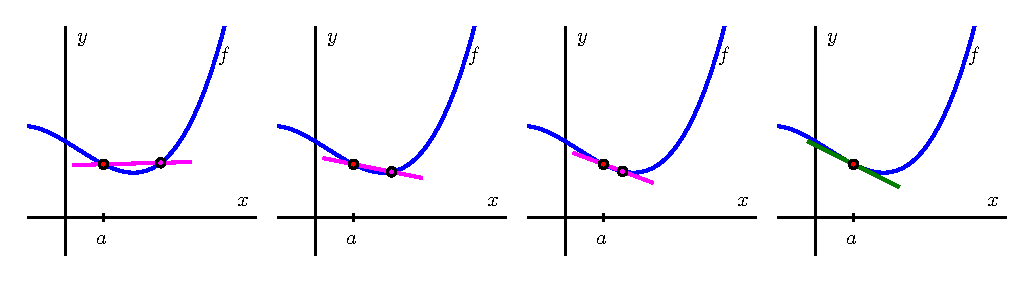
\includegraphics{figures/1_3_SecToTanSeq.eps} %figure ACTIVE
\caption{A sequence of secant lines approaching the tangent line to $f$ at $(a,f(a))$.} \label{fig:2.1.SeqToTanSeq}
\end{center}
\end{figure*}

In Figure~\ref{fig:2.1.SeqToTanSeq}, we provide a sequence of figures with several different lines through the points $(a, f(a))$ and $(a+h,f(a+h))$ that are generated by different values of $h$.  These lines (shown in the first three figures in magenta), are often called \emph{secant lines} \index{secant line} to the curve $y = f(x)$.  A secant line to a curve is simply a line that passes through two points that lie on the curve.  For each such line, the slope of the secant line is $m = \frac{f(a+h) - f(a)}{h}$, where the value of $h$ depends on the location of the point we choose.  We can see in the diagram how, as $h \to 0$, the secant lines start to approach a single line that passes through the point $(a,f(a))$.  In the situation where the limit of the slopes of the secant lines exists, we say that the resulting value is the slope of the \emph{tangent line} to the curve.  This tangent line\index{tangent line} (shown in the right-most figure in green) to the graph of $y = f(x)$ at the point $(a,f(a))$ is the line through $(a,f(a))$ whose slope is $m = f'(a)$.  

\begin{marginfigure} % MARGIN FIGURE
\margingraphics{figures/1_3_SecToTan.eps} %FIGURE ACTIVE 
\caption{A sequence of secant lines approaching the tangent line to $f$ at $(a,f(a))$.  At right, we zoom in on the point $(a,f(a))$.  The slope of the tangent line (in green) to $f$ at $(a,f(a))$ is given by $f'(a)$.} \label{fig:2.1.SeqToTan}
\end{marginfigure}

As we will see in subsequent study, the existence of the tangent line at $x = a$ is connected to whether or not the function $f$ looks like a straight line when viewed up close at $(a,f(a))$, which can also be seen in Figure~\ref{fig:2.1.SeqToTan}, where we combine the four graphs in Figure~\ref{fig:2.1.SeqToTanSeq} into the single one on the left, and then we zoom in on the box centered at $(a,f(a))$, with that view expanded on the right (with two of the secant lines omitted).  Note how the tangent line sits relative to the curve $y = f(x)$ at $(a,f(a))$ and how closely it resembles the curve near $x = a$.

At this time, it is most important to note that $f'(a)$, the instantaneous rate of change of $f$ with respect to $x$ at $x = a$, also measures the slope of the tangent line\index{tangent line!slope} to the curve $y = f(x)$ at $(a,f(a))$.  The following example demonstrates several key ideas involving the derivative of a function.

\begin{example} \label{Ex:2.1.Eg1}
For the function given by $f(x) = x - x^2$, use the limit definition of the derivative to compute $f'(2)$.  In addition, discuss the meaning of this value and draw a labeled graph that supports your explanation. 

\solution From the limit definition, we know that
$$f'(2) = \lim_{h \to 0} \frac{f(2+h)-f(2)}{h}.$$
Now we use the rule for $f$, and observe that $f(2) = 2 - 2^2 = -2$ and $f(2+h) = (2+h) - (2+h)^2.$  Substituting these values into the limit definition, we have that
$$f'(2) = \lim_{h \to 0} \frac{(2+h) - (2+h)^2 -  (-2)}{h}.$$
Observe that with $h$ in the denominator and our desire to let $h \to 0$, we have to wait to take the limit (that is, we wait to actually let $h$ approach $0$).  Thus, we do additional algebra.  Expanding and distributing in the numerator,
$$f'(2) = \lim_{h \to 0} \frac{2+h - 4 - 4h - h^2 + 2}{h}.$$
Combining like terms, we have
$$f'(2) = \lim_{h \to 0} \frac{ -3h - h^2}{h}.$$
Next, we observe that there is a common factor of $h$ in both the numerator and denominator, which allows us to simplify and find that
$$f'(2) = \lim_{h \to 0} (-3-h).$$
Finally, we are able to take the limit as $h \to 0$, and thus conclude that $f'(2) = -3$.

Now, we know that $f'(2)$ represents the slope of the tangent line to the curve $y = x - x^2$ at the point $(2,-2)$; $f'(2)$ is also the instantaneous rate of change of $f$ at the point $(2,-2)$.  Graphing both the function and the line through $(2,-2)$ with slope $m = f'(2) = -3$, we indeed see that by calculating the derivative, we have found the slope of the tangent line at this point, as shown in Figure~\ref{fig:2.1.Eg1}.
\end{example}

\begin{marginfigure}[-6cm]
\margingraphics{figs/2/2-1_Eg1.pdf} %Tangent line ex 1.3 active
\caption{The tangent line to $y = x - x^2$ at the point $(2,-2)$.}\label{fig:2.1.Eg1}
\end{marginfigure} % EXAMPLE

\begin{marginfigure}[1cm]
\margingraphics{figures/figtangent1} %FIG EXAMPLE 33 apex
\caption{A graph of $f(x) = 3x^2+5x-7$ and its tangent lines at $x=1$ and $x=3$.}\label{fig:2.1.Eg3}
\end{marginfigure}

\begin{example} \label{Ex:2.1.Eg3}
Let $f(x) = 3x^2+5x-7$. Find: 
\begin{enumerate*}[1)]
\item $f'(1)$; 	
\item the equation of the tangent line to the graph of $f$ at $x=1$; 
\item $f'(3)$; and 
\item the equation of the tangent line to the graph $f$ at $x=3$.
\end{enumerate*}
	
\solution
\begin{enumerate}[1)]
\item We compute this directly using the definition of the derivative at a point.
\begin{align*}
f'(1) &= \lim_{h \to 0} \frac{f(1+h)-f(1)}{h} \\
&=	\lim_{h \to 0} \frac{3(1+h)^2+5(1+h)-7 - (3(1)^2+5(1)-7)}{h}\\
&=	\lim_{h\to 0} \frac{3h^2+11h}{h}\\
&= 	\lim_{h\to 0} 3h+11=11.
%&= 11.
\end{align*}

\item The tangent line at $x=1$ has slope $f'(1)$ and goes through the point $(1,f(1)) = (1,1)$. Thus the tangent line has equation, in point-slope form, $y = 11(x-1) + 1$. In slope-intercept form we have $y = 11x-10$.
	
\item Again, using the definition,
\begin{align*}
f'(3) &=	\lim_{h \to 0} \frac{f(3+h)-f(3)}{h} \\
&=	\lim_{h \to 0} \frac{3(3+h)^2+5(3+h)-7 - (3(3)^2+5(3)-7)}{h} \\
&=	\lim_{h \to 0} \frac{3h^2+23h}{h}\\
&= \lim_{h \to 0} 3h+23 = 23
%&= 23.
\end{align*}
	
\item The tangent line at $x=3$ has slope $23$ and goes through the point $(3,f(3)) = (3,35)$. Thus the tangent line has equation $y=23(x-3)+35 = 23x-34$.
\end{enumerate}
\end{example} % EXAMPLE APEX example 31

The following activities will help you explore a variety of key ideas related to derivatives.

\begin{activity} \label{A:2.1.1}
Consider the function $f$ whose formula is $\ds f(x) = 3 - 2x$.
\ba
	\item What familiar type of function is $f$?  What can you say about the slope of $f$ at every value of $x$?
	\item Compute the average rate of change of $f$ on the intervals $[1,4]$, $[3,7]$, and $[5,5+h]$; simplify each result as much as possible.  What do you notice about these quantities?
	\item Use the limit definition of the derivative to compute the exact instantaneous rate of change of $f$ with respect to $x$ at the value $a = 1$.  That is, compute $f'(1)$ using the limit definition.  Show your work.  Is your result surprising?
	\item Without doing any additional computations, what are the values of $f'(2)$, $f'(\pi)$, and $f'(-\sqrt{2})$?  Why?
\ea
\end{activity}
\begin{smallhint}
\ba
	\item If $f(x) = 3x^2 + 2x - 4$, we say ``$f$ is quadratic.''  If $f(x) = 5 e^{2x-1}$, we say ``$f$ is exponential.''  What do we say about $f(x) = 3-2x$.  
	\item Remember that to compute the average rate of change of $f$ on $[a,b]$, we calculate $\frac{f(b)-f(a)}{b-a}$.
	\item Observe that $f(1+h) = 3 - 2(1+h) = 3 - 2 - 2h = 1 - 2h$.
	\item Think about the how the graph of $f$ appears.  What is the same at every point?
\ea
\end{smallhint}
\begin{bighint}
\ba
	\item Observe that the function $f$ is of the form $f(x) = mx + b$.
	\item To compute the average rate of change of $f$ on $[1,4]$, we calculate $\frac{f(4)-f(1)}{4-1}$.
	\item Note that $f(1+h) - f(1) = (3 - 2(1+h)) - (3-2) = 3 - 2 - 2h - 1 = -2h$.
	\item Remember that $f'(a)$ represents the slope of the function $f$ at the value $a$.
\ea
\end{bighint}
\begin{activitySolution}
\ba
	\item Because $f(x) = 3 - 2x$ is of the form $f(x) = mx + b$, we call $f$ a \emph{linear} function.
	\item The average rate of change on $[1,4]$ is $\frac{f(4)-f(1)}{4-1} = \frac{-5 - 1}{3} = -2$.  Similar calculations show the average rate of change on $[3,7]$ is also $-2$.  On $[5,5+h]$, observe that 
	$$\frac{f(5+h)-f(5)}{h} = \frac{3-2(5+h) - (3-10)}{h} = \frac{3 - 10 - 2h + 7}{h} = \frac{-2h}{h} = -2.$$
	\item Using the limit definition of the derivative, we find that
	\begin{eqnarray*}
		f'(1) & = & \lim_{h \to 0} \frac{f(1+h) - f(1)}{h} \\
			& = & \lim_{h \to 0} \frac{(3 - 2(1+h)) - (3-2)}{h} \\
			& = & \lim_{h \to 0} \frac{3 - 2 - 2h - 1}{h} \\
			& = & \lim_{h \to 0} \frac{-2h}{h} \\
			& = & \lim_{h \to 0} -2 \\
			& = & -2.
	\end{eqnarray*}
\ea
\end{activitySolution}
\aftera % ACTIVITY

\begin{marginfigure}[9cm]	
\margingraphics{figures/1_3_Act2.eps}
\caption{Axes for plotting $y = s(t)$ in Activity~\ref{A:2.1.2}.} \label{fig:2.1.Act2}
\end{marginfigure}

\begin{activity}  \label{A:2.1.2}
A water balloon is tossed vertically in the air from a window.  The balloon's height in feet at time $t$ in seconds after being launched is given by $s(t) = -16t^2 + 16t + 32$. Use this function to respond to each of the following questions.
\ba
	\item Sketch an accurate, labeled graph of $s$ on the axes provided in Figure~\ref{fig:2.1.Act2}.  You should be able to do this without using computing technology.
		
	\item Compute the average rate of change of $s$ on the time interval $[1,2]$.  Include units on your answer and write one sentence to explain the meaning of the value you found.  
	\item Use the limit definition to compute the instantaneous rate of change of $s$ with respect to time, $t$, at the instant $a = 1$.  Show your work using proper notation, include units on your answer, and write one sentence to explain the meaning of the value you found.
	\item On your graph in (a), sketch two lines:  one whose slope represents the average rate of change of $s$ on $[1,2]$, the other whose slope represents the instantaneous rate of change of $s$ at the instant $a=1$.  Label each line clearly.
	\item For what values of $a$ do you expect $s'(a)$ to be positive?  Why?  Answer the same questions when ``positive'' is replaced by ``negative'' and  ``zero.'' 
\ea
\end{activity}
\begin{smallhint}
\ba
	\item Observe that $(t^2 - t - 2) = (t-2)(t+1)$ and that $s(t)$ has its vertex at $t = \frac{1}{2}$.
	\item Recall the formula for average rate of change.
	\item Note that $s(1+h) = -16(1+h)^2 + 16(1+h) + 32$.
	\item Think about a secant line and a tangent line.
	\item A line with positive slope is one that is rising; a line with negative slope is one that is falling.
\ea
\end{smallhint}
\begin{bighint}
\ba
	\item Show that the quadratic function has $t$-intercepts at $(2,0)$ and $(-1,0)$; $s$-intercept $(0,32)$; and vertex at the point where $t = \frac{1}{2}$.
	\item Compute $\frac{s(2)-s(1)}{2-1}$.
	\item Observe that $s(1+h) - s(1) = (-16(1+h)^2 + 16(1+h) + 32) - (-16(1)^2 + 16(1) + 32) = -16 - 32h - 16h^2 + 16 + 16h + 32 - 32$ and combine like terms carefully.
	\item Consider the line through $(1,s(1))$ and $(2,s(2))$, as well as the line through $(1,s(1))$ with slope $s'(1)$.
	\item Observe that whenever the ball is rising, it's position function is rising, and thus the slope of its tangent line at any such point will be positive.
\ea
\end{bighint}
\begin{activitySolution}
\ba
	\item Since $s(t) = -16t^2 + 16t + 32 = -16(t^2 - t - 2) = -16(t-2)(t+1)$, $s$ has $t$-intercepts at $(2,0)$ and $(-1,0)$; the $s$-intercept is clearly $(0,32)$; and the vertex is $(\frac{1}{2},36)$.
	\item Observe that $\frac{s(2)-s(1)}{2-1} = \frac{0 - 32}{1} = -32$ feet per second.  This value represents the average rate at which the ball is falling over the time interval from $t = 1$ to $t = 2$.
	\item We compute $s'(1)$ as follows:
	\begin{eqnarray*}
		s'(1) & = & \lim_{h \to 0} \frac{s(1+h)-s(1)}{h} \\
		       & = & \lim_{h \to 0} \frac{(-16(1+h)^2 + 16(1+h) + 32) - (-16(1)^2 + 16(1) + 32)}{h} \\
		       & = & \lim_{h \to 0} \frac{-16 - 32h - 16h^2 + 16 + 16h + 32 - 32}{h} \\
		       & = & \lim_{h \to 0} \frac{-16h - 16h^2}{h} \\
		       & = & \lim_{h \to 0} (-16-16h) \\
		       & = & -16.
	\end{eqnarray*}  
	\item We plot and label the secant line through $(1,s(1))$ and $(2,s(2))$, as well as the tangent line through $(1,s(1))$ with slope $s'(1)$.

	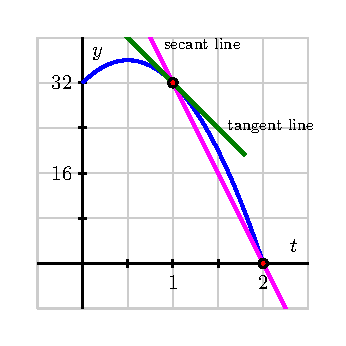
\includegraphics{figures/1_3_Act2Soln.eps}
	
	\item Observe that whenever the ball is rising, it's position function is rising, and thus the slope of its tangent line at any such point will be positive. This means that we should find $s'(a)$ to be positive whenever $0 \le a < \frac{1}{2}$, and similarly $s'(a)$ to be negative whenever $\frac{1}{2} < a < 2$ (which is when the ball is falling).  At the instant $a = \frac{1}{2}$, the ball is at its vertex and is neither rising nor falling, and at that point, $s'(\frac{1}{2}) = 0.$
\ea
\end{activitySolution}
\aftera % ACTIVITY  

\newpage

\begin{marginfigure}[1cm]
\margingraphics{figures/1_3_Act3.eps} 
\caption{Axes for plotting $y = P(t)$ in Activity~\ref{A:2.1.3}.} \label{fig:2.1.Act3}
\end{marginfigure}

\begin{activity}  \label{A:2.1.3}
A rapidly growing city in Arizona has its population $P$ at time $t$, where $t$ is the number of decades after the year $2010$, modeled by the formula $P(t) = 25000 e^{t/5}$.  Use this function to respond to the following questions.
\ba
	\item Sketch an accurate graph of $P$ for $t = 0$ to $t = 5$ on the axes provided in Figure~\ref{fig:2.1.Act3}.  Label the scale on the axes carefully.
	
	\item Compute the average rate of change of $P$ between $2030$ and $2050$.  Include units on your answer and write one sentence to explain the meaning (in everyday language) of the value you found.
	\item Use the limit definition to write an expression for the instantaneous rate of change of $P$ with respect to time, $t$, at the instant $a = 2$.  Explain why this limit is difficult to evaluate exactly.  
	\item Estimate the limit in (c) for the instantaneous rate of change of $P$ at the instant $a = 2$ by using several small $h$ values.  Once you have determined an accurate estimate of $P'(2)$, include units on your answer, and write one sentence (using everyday language) to explain the meaning of the value you found.
	\item On your graph above, sketch two lines:  one whose slope represents the average rate of change of $P$ on $[2,4]$, the other whose slope represents the instantaneous rate of change of $P$ at the instant $a=2$.
	\item In a carefully-worded sentence, describe the behavior of $P'(a)$ as $a$ increases in value.  What does this reflect about the behavior of the given function $P$?
\ea
\end{activity}
\begin{smallhint}
\ba
	\item $P(t)$ is the standard exponential function, scaled by $25000$.
	\item Use the formula for the average rate of change of a function.
	\item Because of the exponential nature of $P(t)$, we're not able to simplify $\frac{P(2+h)-P(2)}{h}$ in a way that removes $h$ from the denominator.  
	\item Try using $h = 0.001, 0.0001, 0.00001$ and $h = -0.001, -0.0001, -0.00001$.  Be careful not to round or use computing precision that is too limited.  
	\item For the first line, think about the points $(2,P(2))$ and $(4,P(4))$.
	\item Visualize the slope of the tangent line and how it changes as a point moves along the curve.
\ea
\end{smallhint}
\begin{bighint}
\ba
	\item $P(t)$ is the standard exponential function, scaled by $25000$.
	\item Remember that $AV_{[2,4]} = \frac{P(4)-P(2)}{4-2}$, and that the units on $P$ are people, while $t$ is the number of decades after 2010. 
	\item Note that
	$$P'(2) = \lim_{h \to 0} \frac{P(2+h)-P(2)}{h} = \lim_{h \to 0} \frac{25000 e^{2+h}-25000e^2}{h}.$$  
	\item Try using $h = 0.001, 0.0001, 0.00001$ and $h = -0.001, -0.0001, -0.00001$.  Be careful not to round or use computing precision that is too limited.  Think about how using the two values of $h$ nearest 0 together could give you the most accurate result.
	\item For the first line, think about the points $(2,P(2))$ and $(4,P(4))$.  For the second, try the line through $(2,P(2))$ with slope $P'(2)$.
	\item Visualize the slope of the tangent line and how it changes as a point moves along the curve.  Does the slope of the tangent line increase, decrease, or stay the same as the point of tangency moves along the curve from right to left?
\ea
\end{bighint}
\begin{activitySolution}
\ba
	\item 	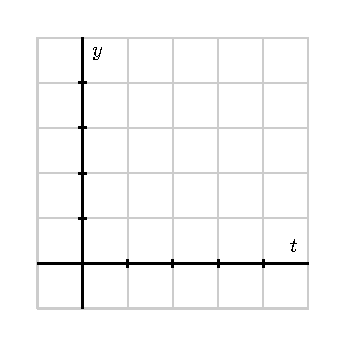
\includegraphics{figures/1_3_Act3.eps}
	\item $AV_{[2,4]} = \frac{P(4)-P(2)}{4-2} = \frac{25000e^{4/5} - 25000e^{2/5}}{2} \approx 9171$ people per decade is expected to be the average rate of change of the city's population over the two decades from 2030 to 2050.
	\item Note that
	\begin{eqnarray*} P'(2) & = & \lim_{h \to 0} \frac{P(2+h)-P(2)}{h} = \lim_{h \to 0} \frac{25000 e^{(2+h)/5}-25000e^{2/5}}{h} \\
	                                 & = &  \lim_{h \to 0} \frac{25000 e^{2/5} e^{h/5} -25000e^{2/5}}{h} =  \lim_{h \to 0} 25000e^{2/5}\left( \frac{e^{h/5} - 1}{h}\right)	\end{eqnarray*}
Because there is no way to remove a factor of $h$ from the numerator, we cannot eliminate the $h$ that is making the denominator go to zero, so it appears we need to be content estimating the limit with small values of $h$.
	\item Using $h = 0.00001$, we find $\frac{P(2+0.00001)-P(2)}{0.00001} \approx 7457$; using $h = -0.00001$, we find $\frac{P(2-0.00001)-P(2)}{-0.00001} \approx 7460$.  Averaging these two results, we find that
	$$P'(2) =  \lim_{h \to 0} \frac{P(2+h)-P(2)}{h} \approx 7458.5$$
	which is measured in people per decade.
	\item See the graph provided in (a) above.  The magenta line has slope equal to the average rate of change of $P$ on $[2,4]$, while the green line is the tangent line at $(2,P(2))$ with slope $P'(2)$.
	\item If we consider the point where $t = a$ and let $a$ start at 0 and then increase, it appears that the tangent line's slope at the point $(a,P(a))$ will increase as $a$ increases.
\ea
\end{activitySolution}
\aftera % ACTIVITY

%------------------------------------------------------------------
% SUBSECTION UNITS OF THE DERIVATIVE FUNCTION
%------------------------------------------------------------------
\subsection*{Units of the derivative function}

As we now know, the derivative of the function $f$ at a fixed value $x$ is given by
$$f'(x) = \ds \lim_{h \to 0} \frac{f(x+h)-f(x)}{h},$$  and this value has several different interpretations.  If we set $x = a$, one meaning of $f'(a)$ is  the slope of the tangent line at the point $(a,f(a))$.

In alternate notation, we also sometimes equivalently write $\frac{df}{dx}$ or $\frac{dy}{dx}$ instead of $f'(x)$, and these notations help us to further see the units (and thus the meaning) of the derivative as it is viewed as \emph{the instantaneous rate of change of $f$ with respect to $x$}\index{instantaneous rate of change}.  Note that the units on the slope of the secant line, $\frac{f(x+h)-f(x)}{h}$, are ``units of $f$ per unit of $x$.''  Thus, when we take the limit to get $f'(x)$, we get these same units on the derivative $f'(x)$:  units of $f$ per unit of $x$.  Regardless of the function $f$ under consideration (and regardless of the variables being used), it is helpful to remember that the units on the derivative function are ``units of output per unit of input,'' in terms of the input and output of the original function.

For example, say that we have a function $y = P(t)$, where $P$ measures the population of a city (in thousands) at the start of year $t$ (where $t = 0$ corresponds to $2010$ AD), and we are told that $P'(2) = 21.37$.  What is the meaning of this value?  Well, since $P$ is measured in thousands and $t$ is measured in years, we can say that the instantaneous rate of change of the city's population with respect to time at the start of $2012$ is $21.37$ thousand people per year.  We therefore expect that in the coming year, about $21,370$ people will be added to the city's population.

%----------------------------------------------------
% SUBSECTION ESTIMATING DERIVATIVES 
%----------------------------------------------------
\subsection*{Estimating Derivatives}

An interesting and powerful feature of mathematics is that it can often be thought of both in abstract terms and in applied ones.  For instance, calculus can be developed almost entirely as an abstract collection of ideas that focus on properties of arbitrary functions.  At the same time, calculus can also be very directly connected to our experience of physical reality by considering functions that represent meaningful processes.  We have already seen that for a position function $y = s(t)$, say for a ball being tossed straight up in the air, the ball's velocity at time $t$ is given by $v(t) = s'(t)$, the derivative of the position function.  Further, recall that if $s(t)$ is measured in feet at time $t$, the units on $v(t) = s'(t)$ are feet per second.

In what follows, we investigate several different functions, each with specific physical meaning, and think about how the units on the independent variable, dependent variable, and the derivative function add to our understanding.  To start, we consider the familiar problem of a position function of a moving object.

\begin{marginfigure}[8cm]
\margingraphics{figures/1_5_PA1.eps}
\caption{The graph of $y = s(t)$, the position of the car along highway $46$, which tells its distance in miles from Gackle, ND, at time $t$ in minutes.} \label{fig:2.1.Act4}
\end{marginfigure}

\begin{activity}  \label{A:2.1.4}
One of the longest stretches of straight (and flat) road in North America can be found on the Great Plains in the state of North Dakota on state highway $46$, which lies just south of the interstate highway I-$94$ and runs through the town of Gackle.  A car leaves town (at time $t = 0$) and heads east on highway $46$; its position in miles from Gackle at time $t$ in minutes is given by the graph of the function in Figure~\ref{fig:2.1.Act4}.  Three important points are labeled on the graph; where the curve looks linear, assume that it is indeed a straight line.

\ba
	\item In everyday language, describe the behavior of the car over the provided time interval.  In particular, discuss what is happening on the time intervals $[57,68]$ and $[68,104]$.
	\item Find the slope of the line between the points $(57,63.8)$ and $(104,106.8)$.  What are the units on this slope?  What does the slope represent?
	\item Find the average rate of change of the car's position on the interval $[68,104]$.  Include units on your answer.
	\item Estimate the instantaneous rate of change of the car's position at the moment $t = 80$.  Write a sentence to explain your reasoning and the meaning of this value.
\ea
\end{activity} % ACTIVITY

%-----------------------------------------------------------------------------------
% SUBSECTION TOWARD MORE ACCURATE DERIVATIVE ESTIMATES
%-----------------------------------------------------------------------------------
\subsection*{Toward more accurate derivative estimates}

It is also helpful to recall that when we want to estimate the value of $f'(x)$ at a given $x$, we can use the \emph{difference quotient} \index{difference quotient} $\frac{f(x+h)-f(x)}{h}$ with a relatively small value of $h$.  In doing so, we should use both positive and negative values of $h$ in order to make sure we account for the behavior of the function on both sides of the point of interest.  To that end, we consider the following brief example to demonstrate the notion of a \emph{central difference} and its role in estimating derivatives.

\begin{example} \label{Ex:2.1.Eg2}
Suppose that $y = f(x)$ is a function for which three values are known:  $f(1) = 2.5$, $f(2) = 3.25$, and $f(3) = 3.625$.  Estimate $f'(2)$.

\solution We know that $\ds f'(2) = \lim_{h \to 0} \frac{f(2+h) - f(2)}{h}$.  But since we don't have a graph for $y = f(x)$ nor a formula for the function, we can neither sketch a tangent line nor evaluate the limit exactly.  We can't even use smaller and smaller values of $h$ to estimate the limit.  Instead, we have just two choices:  using $h = -1$ or $h = 1$, depending on which point we pair with $(2,3.25)$.

So, one estimate is
$$f'(2) \approx \frac{f(1)-f(2)}{1-2} = \frac{2.5-3.25}{-1} = 0.75.$$
The other is
$$f'(2) \approx \frac{f(3)-f(2)}{3-2} = \frac{3.625-3.25}{1} = 0.375.$$
Since the first approximation looks only backward from the point $(2,3.25)$ and the second approximation looks only forward from $(2,3.25)$, it makes sense to average these two values in order to account for behavior on both sides of the point of interest.  Doing so, we find that
$$f'(2) \approx \frac{0.75 + 0.375}{2} = 0.5625.$$
\end{example} % EXAMPLE

\begin{marginfigure}[1cm] % MARGIN FIGURE
\margingraphics{figures/1_5_Ex1.eps}
\caption{At left, the graph of $y = f(x)$ along with the secant line through $(1,2.5)$ and $(2,3.25)$, the secant line through $(2, 3.25)$ and $(3,3.625)$, as well as the tangent line.  At right, the same graph along with the secant line through $(1,2.5)$ and $(3,3.625)$, plus the tangent line.}\label{fig:2.1.Eg2}
\end{marginfigure}

The intuitive approach to average the two estimates found in Example~\ref{Ex:2.1.Eg2} is in fact the best possible estimate to $f'(2)$ when we have just two function values for $f$ on opposite sides of the point of interest.  To see why, we think about the diagram in Figure~\ref{fig:2.1.Eg2}, which shows a possible function $y = f(x)$ that satisfies the data given in Example~\ref{Ex:2.1.Eg2}.  On the left, we see the two secant lines with slopes that come from computing the \emph{backward difference} \index{backward difference} $\frac{f(1)-f(2)}{1-2} = 0.75$ and from the \emph{forward difference} \index{forward difference} $\frac{f(3)-f(2)}{3-2} = 0.375.$  Note how the first such line's slope over-estimates the slope of the tangent line at $(2,f(2))$, while the second line's slope underestimates $f'(2)$.  On the right, however, we see the secant line whose slope is given by the \emph{central difference} \index{central difference} 
\[ \frac{f(3)-f(1)}{3-1} = \frac{3.625-2.5}{2} = \frac{1.125}{2} = 0.5625.\]

Note that this central difference has the exact same value as the average of the forward difference and backward difference (and it is straightforward to explain why this always holds), and moreover that the central difference yields a very good approximation to the derivative's value, in part because the secant line that uses both a point before and after the point of tangency yields a line that is closer to being parallel to the tangent line.  

In general, the central difference approximation to the value of the first derivative is given by 
$$f'(a) \approx \frac{f(a+h) - f(a-h)}{2h},$$
and this quantity measures the slope of the secant line to $y = f(x)$ through the points $(a-h, f(a-h))$ and $(a+h, f(a+h))$. Anytime we have symmetric data surrounding a point at which we desire to estimate the derivative, the central difference is an ideal choice for so doing.

The following activities will further explore the meaning of the derivative in several different contexts while also viewing the derivative from graphical, numerical, and algebraic perspectives.

\begin{margintable}[8cm]
\begin{center}
\scalebox{1.5}{
\begin{tabular}{| l || l |}
\hline
$t$ & $F(t)$ \\ \hline \hline
$0$ & $70$\\ \hline
$15$ & $180.5$ \\ \hline
$30$ & $251$ \\ \hline
$45$ & $296$ \\ \hline
$60$ & $324.5$ \\ \hline
$75$ & $342.8$ \\ \hline
$90$ & $354.5$  \\ \hline
\end{tabular}
} % end scalebox 
\caption{The temperature of a potato in an oven at various times.} \label{T:2.1.5}
\end{center}
\end{margintable}

\begin{activity} \label{A:2.1.5}
A potato is placed in an oven, and the potato's temperature $F$ (in degrees Fahrenheit) at various points in time is taken and recorded in Table~\ref{T:2.1.5}. Time $t$ is measured in minutes.

\ba
	\item Use a central difference to estimate the instantaneous rate of change of the temperature of the potato at $t= 30$. Include units on your answer. 
	\item Use a central difference to estimate the instantaneous rate of change of the temperature of the potato at $t= 60$. Include units on your answer. 
	\item Without doing any calculation, which do you expect to be greater: $F'(75)$ or $F'(90)$?  Why?
	\item Suppose it is given that $F(64) = 330.28$ and $F'(64) = 1.341$.  What are the units on these two quantities?  What do you expect the temperature of the potato to be when $t = 65$?  when $t = 66$?  Why?
	\item Write a couple of careful sentences that describe the behavior of the temperature of the potato on the time interval $[0,90]$, as well as the behavior of the instantaneous rate of change of the temperature of the potato on the same time interval.
\ea

\end{activity}
\begin{smallhint}
\ba
	\item Think about quantities such as $\frac{F(45)-F(30)}{45-30}$.
	\item See the note in (a).
	\item Is $F$ changing faster at $t = 75$ or at $t = 90$?
	\item Remember that the units on $F'$ will be ``degrees Fahrenheit per minute.''
	\item Be careful to distinguish between the temperature, $F$, and the rate of change of temperature, $F'$, in your commentary.
\ea
\end{smallhint}
\begin{bighint}
\ba
	\item Think about quantities such as $\frac{F(45)-F(30)}{45-30}$ and $\frac{F(15)-F(30)}{15-30}$.
	\item See the note in (a).
	\item What overall trend do you observe in the instantaneous rate of change of $F$, based on the overall trend in temperature $F$?
	\item Remember that the units on $F'$ will be ``degrees Fahrenheit per minute.''
	\item Be careful to distinguish between the temperature, $F$, and the rate of change of temperature, $F'$, in your commentary.
\ea
\end{bighint}
\begin{activitySolution}
\ba
	\item Using the central difference, we find that 
	$$F'(30) \approx \frac{F(45)-F(15)}{45-15} = \frac{296-180.5}{30} = 3.85$$
	degrees per minute.
	\item Using the central difference, we find that 
	$$F'(60) \approx \frac{F(75)-F(45)}{45-15} = \frac{342.8-296}{30} = 1.56$$
	degrees per minute.
	\item Over each subsequent time interval, we see that the amount of increase in the potato's temperature gets less and less, thus we expect the value of $F'(t)$ to get smaller and smaller as time goes on.  We therefore expect $F'(75) > F'(90)$.
	\item The value $F(64) = 330.28$ is the temperature of the potato in degrees Fahrenheit at time 64, while $F'(64) = 1.341$ measures the instantaneous rate of change of the potato's temperature with respect to time at the instant $t = 64$, and its units are degrees per minute.  Because at time $t = 64$ the potato's temperature is increasing at 1.341 degrees per minute, we expect that at $t = 65$, the temperature will be about 1.341 degrees greater than at $t = 64$, or in other words $F(65) \approx 330.28 + 1.341 = 331.621$.  Similarly, at $t = 66$, two minutes have elapsed from $t = 64$, so we expect an increase of $2 \dot 1.341$ degrees:  $F(66) \approx 330.28 + 2 \cdot 1.341 = 332.962$. 
	\item Throughout the time interval $[0,90]$, the temperature $F$ of the potato is increasing.  But as time goes on, the rate at which the temperature is rising appears to be decreasing.  That is, while the values of $F$ continue to get larger as time progresses, the values of $F'$ are getting smaller (while still remaining positive). We thus might say that ``the temperature of the potato is increasing, but at a decreasing rate.''
\ea
\end{activitySolution}
\aftera %ACTIVITY

\begin{example} \label{Ex:2.1.Eg4}
A company manufactures rope, and the total cost of producing $r$ feet of rope is $C(r)$ dollars.  What does it mean to say that $C(2000) = 800$? What are the units of $C'(r)$? Suppose that $C(2000) = 800$ and $C'(2000) = 0.35$.  Estimate $C(2100)$, and justify your estimate by writing at least one sentence that explains your thinking. Which of the following statements do you think is true, and why?
	\begin{itemize}
		\item $C'(2000) < C'(3000)$
		\item $C'(2000) = C'(3000)$
		\item $C'(2000) > C'(3000)$
	\end{itemize}
Suppose someone claims that $C'(5000) = -0.1$.  What would the practical meaning of this derivative value tell you about the approximate cost of the next foot of rope?  Is this possible?  Why or why not?  
	
\solution When we say $C(2000) = 800$, we mean that the total cost of producing $2000$ feet of rope is $800$ dollars.  Remember that the units on any derivative are ``units of output per unit of input,'' and the units of $C'(r)$ are ``dollars per foot.''

If $C(2000) = 800$ and $C'(2000) = 0.35$, then we know once $2000$ feet of rope are produced, the total cost function is increasing at $\$0.35$ per additional foot of rope.  Then, if we manufacture an additional $100$ feet of rope, the additional total cost will be approximately 
\[ 100 \ \mbox{feet} \cdot 0.35 \ \frac{\mbox{dollars}}{\mbox{foot}} = 35 \ \mbox{dollars}. \]
Therefore, we find that $C(2100) \approx C(2000) + 35 = 835,$ or that the cost to make $2100$ feet of rope is about $\$835$.

Either $C'(2000) = C'(3000)$ or $C'(2000) > C'(3000)$, since we expect the cost per foot of additional rope to either stay constant or to get smaller as the production volume increases.  Said differently, the instantaneous rate of change of the total cost function should either be constant or decrease due to economy of scale.

It is impossible to have $C'(5000) = -0.1$ and indeed to have any negative derivative value for the total cost function.  The total cost function $C(r)$ can never decrease, because it doesn't make sense for the total cost of producing $5001$ feet of rope to be less than the total cost of producing $5000$ feet of rope.

\end{example} %ACTIVITY  %this is a lot of activities we may need to narrow

\begin{activity} \label{A:2.1.7}
Researchers at a major car company have found a function that relates gasoline consumption to speed for a particular model of car.  In particular, they have determined that the consumption $C$, in {\bfseries liters per kilometer}, at a given speed $s$, is given by a function $C = f(s)$, where $s$ is the car's speed in {\bf kilometers per hour}. 
	\ba
	  \item Data provided by the car company tells us that $f(80) = 0.015$, $f(90) = 0.02$, and $f(100) = 0.027$.  Use this information to estimate the instantaneous rate of change of fuel consumption with respect to speed at $s = 90$.  Be as accurate as possible, use proper notation, and include units on your answer.
	  \item By writing a complete sentence, interpret the meaning (in the context of fuel consumption) of ``$f(80) = 0.015$.'' 
	  \item Write at least one complete sentence that interprets the meaning of the value of $f'(90)$ that you estimated in (a).
	\ea
\end{activity}
\begin{smallhint}
\ba
	\item Try a central difference.
	\item What is happening when the car is traveling at 80 km/hr?
	\item Remember that units on the derivative are ``units of output per unit of input.''
\ea
\end{smallhint}
\begin{bighint}
\ba
	\item Remember that $f'(a) \approx \frac{f(a+h)-f(a-h)}{2h}$ and use appropriate values of $a$ and $h$.
	\item Complete the following sentence: ``When the car is traveling at 80 kilometers per hour, it is using fuel at a rate of 0.015 $\ldots$''
	\item Remember that units on the derivative are ``units of output per unit of input,'' even when the input and/or output are rates themselves.
\ea
\end{bighint}
\begin{activitySolution}
\ba
	\item Using a central difference, we have
	$$f'(90) = \frac{f(100) - f(80}{100-80} = \frac{0.027 - 0.015}{20} = \frac{0.012}{20} = 0.0006$$
	which tells us that $f'(90) = 0.0006$ liters per kilometer per kilometer per hour.
	\item When the car is traveling at 80 kilometers per hour, it is using fuel at a rate of 0.015 liters per kilometer.  That is, at the given speed, for each additional kilometer the car travels, it uses an additional 0.015 liters of fuel.
	\item To say that $f'(90) = 0.0006$ liters per kilometer per kilometer per hour means that when the car is traveling at 90 kilometers per hour, its rate of fuel consumption per kilometer is increasing at a rate of 0.0006 liters per kilometer per kilometer per hour.  If we increase our speed from 90 to 91 km/hr, we would expect our rate of fuel consumption to rise by 0.0006 liters for each additional kilometer driven.
\ea
\end{activitySolution}
\aftera %ACTIVITY

%--------------
% SUMMARY
%--------------
\begin{summary}
\item The average rate of change of a function $f$ on the interval $[a,b]$ is $\ds \frac{f(b)-f(a)}{b-a}$.  The units on the average rate of change are units of $f$ per unit of $x$, and the numerical value of the average rate of change represents the slope of the secant line between the points $(a,f(a))$ and $(b,f(b))$ on the graph of $y = f(x)$.  If we view the interval as being $[a,a+h]$ instead of $[a,b]$, the meaning is still the same, but the average rate of change is now computed by  $\ds \frac{f(a+h)-f(a)}{h}$.

\item The instantaneous rate of change with respect to $x$ of a function $f$ at a value $x = a$ is denoted $f'(a)$ (read ``the derivative of $f$ evaluated at $a$'' or ``$f$-prime at $a$'') and is defined by the formula
$$f'(a) = \lim_{h \to 0} \frac{f(a+h)-f(a)}{h},$$
provided the limit exists.  Note particularly that the instantaneous rate of change at $x = a$ is the limit of the average rate of change on $[a,a+h]$ as $h \to 0$.

\item Provided the derivative $f'(a)$  exists, its value tells us the instantaneous rate of change of $f$ with respect to $x$ at $x = a$, which geometrically is the slope of the tangent line to the curve $y = f(x)$ at the point $(a,f(a))$.  We even say that $f'(a)$ is the \emph{slope of the curve} $y = f(x)$ at the point $(a,f(a))$.

\item Limits are the link between average rate of change and instantaneous rate of change: they allow us to move from the rate of change over an interval to the rate of change at a single point.

%\item Regardless of the context of a given function $y=f(x)$, the derivative always measures the instantaneous rate of change of the output variable with respect to the input variable.

%\item The units on the derivative function $y = f'(x)$ are units of $f$ per unit of $x$.  Again, this measures how fast the output of the function $f$ changes when the input of the function changes.

\item The central difference approximation to the value of the first derivative is given by 
$$f'(a) \approx \frac{f(a+h) - f(a-h)}{2h},$$
and this quantity measures the slope of the secant line to $y = f(x)$ through the points $(a-h, f(a-h))$ and $(a+h, f(a+h))$.  The central difference generates a good approximation of the derivative's value any time we have symmetric data surrounding a point of interest.

\item Knowing the derivative and function values at a single point enables us to estimate other function values nearby.  If, for example, we know that $f'(7) = 2$, then we know that at $x = 7$, the function $f$ is increasing at an instantaneous rate of $2$ units of output for every one unit of input.  Thus, we expect $f(8)$ to be approximately $2$ units greater than $f(7)$.  The value is approximate because we don't know that the rate of change stays the same as $x$ changes.
\end{summary}

\clearpage

%--------------
% EXERCISES
%--------------
\begin{adjustwidth*}{}{-2.25in}
\textbf{{\large Exercises}}
\setlength{\columnsep}{25pt}
\begin{multicols*}{2}
\noindent Terms and Concepts \small
\begin{enumerate}[1)]
\item {T/F: Let $f$ be a position function. The average rate of change on $[a,b]$ is the slope of the line through the points $(a, f(a))$ and $(b,f(b))$.}
\item {T/F: The definition of the derivative of a function at a point involves taking a limit.}
\item {In your own words, explain the difference between the average rate of change and instantaneous rate of change.}
\item What is the instantaneous rate of change of position called?
\item Given a function $y=f(x)$, in your own words describe how to find the units of $f'(x)$.
\item Let $V(x)$ measure the volume, in decibels, measured inside a restaurant with $x$ customers. What are the units of $V'(x)$?
\item Let $v(t)$ measure the velocity, in ft/s, of a car moving in a straight line $t$ seconds after starting. What are the units of $v'(t)$?
\end{enumerate} 

\noindent {\normalsize Problems} \small

\noindent {\bf In exercises 8--14, a function and an $x$-value $a$ are given.
\begin{enumerate}[a),leftmargin=12pt]
\item Find the derivative of the function at the given point.
\item Find the tangent line to the graph of the function at $a$.
\end{enumerate}}

\begin{enumerate}[1),resume]
\item $\ds f(x) = 6; \quad a = -2$
\item $\ds f(x) = 2x; \quad a = 3$
\item $\ds h(x) = 4 - 3x; \quad a = 7$
\item $\ds g(x) = x^2; \quad a = 2$
\item $\ds f(x) = 3x^2 - x + 4; \quad a = -1$
\item $\ds h(x) = \frac{1}{x}; \quad a = -2$
\item $\ds r(x) = \frac{1}{x-2}; \quad a = 3$
\end{enumerate}

\noindent {\bf In exercises 15--17, use a central difference to estimate the instantaneous rates of change at the indicated values.}
\begin{enumerate}[1),resume]
\item The yearly profits $P(t)$, in millions of dollars, of a certain company from $1990$ to $1996$ are given in the following table.

\scalebox{0.85}{\begin{tabular}{|c|c|c|c|c|c|c|c|}
\hline
Year & $1990$ & $1991$ & $1992$ & $1993$ & $1994$ & $1995$ & $1996$ \\ \hline
Profit & $0.5$ & $1.0$ & $1.2$ & $1.6$ & $2.5$ & $1.6$ & $2.0$ \\ \hline
\end{tabular}}% end scalebox

Estimate $P'(1991)$, $P'(1993)$, and $P'(1995)$.  Include units in your answers.

\item The position, $s(t)$, of an object moving in a straight line at time $t$ is given by the following table.

\begin{center}
\scalebox{0.85}{\begin{tabular}{|c|c|c|c|c|c|}
\hline
$t$ & $0$ & $0.5$ & $1$ & $1.5$ & $2$  \\ \hline
$s(t)$ & $0$ & $30$ & $52$ & $66$ & $72$  \\ \hline
\end{tabular}}% end scalebox
\end{center}

Estimate $s'(0.5)$, $s'(1)$, and $s'(1.5)$.  Include units in your answers.

\item The average price, $p(t)$, for a ticket to a movie theater in North America for selected years is shown in the following table.

 \scalebox{0.85}{\begin{tabular}{|c|c|c|c|c|c|c|c|}
\hline
Year & $1987$ & $1991$ & $1995$ & $1999$ & $2003$ & $2007$ & $2009$ \\ \hline
Price (\$) & $3.91$ & $4.21$ & $4.35$ & $5.06$ & $6.03$ & $6.88$ & $7.50$ \\ \hline
\end{tabular}}% end scalebox

{\footnotesize (Source: National Association of Theater Owners, www.natoonline.org)}

\ba
\item Estimate $p'(1991)$ and $p'(2003)$.  Include units in your answers.
\item Are we able to estimate $p'(2007)$ using a central difference?  Why or why not?
\ea

\item A cup of coffee has its temperature $F$ (in degrees Fahrenheit) at time $t$ given by the function $F(t) = 75 + 110 e^{-0.05t}$, where time is measured in minutes.
\ba
\item Use a central difference with $h = 0.01$ to estimate the value of $F'(10)$.
\item What are the units on the value of $F'(10)$ that you computed in (a)?  What is the practical meaning of the value of $F'(10)$?
\item Which do you expect to be greater: $F'(10)$ or $F'(20)$?  Why?  
\item Write a sentence that describes the behavior of the function $y = F'(t)$ on the time interval $0 \le t \le 30$.  How do you think its graph will look?  Why?
\ea

\item The temperature change $T$ (in Fahrenheit degrees), in a patient, that is generated by a dose $q$ (in milliliters), of a drug, is given by the function $T = f(q)$.
\ba
\item What does it mean to say $f(50) = 0.75$?  Write a complete sentence to explain, using correct units.
\item A person's sensitivity, $s$, to the drug is defined by the function $s(q) = f'(q)$.  What are the units of sensitivity?
\item Suppose that $f'(50) = -0.02$.  Write a complete sentence to explain the meaning of this value.  Include in your response the information given in (a).
\ea

\end{enumerate}

%------------------------------------------
% END OF EXERCISES ON FIRST PAGE
%------------------------------------------
\end{multicols*}
\end{adjustwidth*}

\clearpage

\begin{adjustwidth*}{}{-2.25in}
\setlength{\columnsep}{25pt}
\begin{multicols*}{2}\small

\begin{enumerate}[1),start=20]
\item The velocity of a ball that has been tossed vertically in the air is given by $v(t) = 16 - 32t$, where $v$ is measured in feet per second, and $t$ is measured in seconds.  The ball is in the air from $t = 0$ until $t = 2$.
\ba
\item When is the ball's velocity greatest?
\item Determine the value of $v'(1)$.  Justify your thinking.
\item What are the units on the value of $v'(1)$?  What does this value and the corresponding units tell you about the behavior of the ball at time $t = 1$?  
\item What is the physical meaning of the function $v'(t)$?
\ea

\item The value, $V$, of a particular automobile (in dollars) depends on the number of miles, $m$, the car has been driven, according to the function $V = h(m)$.  
\ba
\item Suppose that $h(40000) = 15500$ and $h(55000) = 13200$.  What is the average rate of change of $h$ on the interval $[40000,55000]$, and what are the units on this value?
\item In addition to the information given in (a), say that $h(70000) = 11100$.  Determine the best possible estimate of $h'(55000)$ and write one sentence to explain the meaning of your result, including units on your answer.
\item Which value do you expect to be greater: $h'(30000)$ or $h'(80000)$?  Why?
\item Write a sentence to describe the long-term behavior of the function $V = h(m)$, plus another sentence to describe the long-term behavior of $h'(m)$.  Provide your discussion in practical terms regarding the value of the car and the rate at which that value is changing.
\ea

\end{enumerate}

%------------------------------------------------
% END OF EXERCISES ON SECOND PAGE
%------------------------------------------------
\end{multicols*}
\end{adjustwidth*}
\afterexercises 

\cleardoublepage
\section{The derivative function} \label{S:2.2.DerivativeFxn}

\begin{goals}
\item How does the limit definition of the derivative of a function $f$ lead to an entirely new (but related) function $f'$?
\item What is the difference between writing $f'(a)$ and $f'(x)$?
\item How is the graph of the derivative function $f'(x)$ connected to the graph of $f(x)$?
\item What are some examples of functions $f$ for which $f'$ is not defined at one or more points?
\item What does it mean graphically to say that a function $f$ is differentiable at $x = a$?  How is this connected to the function being locally linear? 
\end{goals}

%--------------------------------------
% SUBSECTION INTRODUCTION
%--------------------------------------
\subsection*{Introduction}

Given a function $y = f(x)$, we now know that if we are interested in the instantaneous rate of change of the function at $x = a$, or equivalently the slope of the tangent line to $y = f(x)$ at $x = a$, we can compute the value $f'(a)$.  In all of our examples to date, we have arbitrarily identified a particular value of $a$ as our point of interest: $a = 1$, $a = 3$, etc.  But it is not hard to imagine that we will often be interested in the derivative value for more than just one $a$-value, and possibly for many of them.  In this section, we explore how we can move from computing simply $f'(1)$ or $f'(3)$ to working more generally with $f'(a)$, and indeed $f'(x)$.  Said differently, we will work toward understanding how the so-called process of "taking the derivative" generates a new function that is derived from the original function $y = f(x)$.  The following preview activity starts us down this path.

\begin{pa} \label{PA:1.4}
Consider the function $f(x) = 4x - x^2$.
\ba
	\item Use the limit definition to compute the following derivative values:  $f'(0)$, $f'(1)$, $f'(2)$, and $f'(3)$.
	\item Observe that the work to find $f'(a)$ is the same, regardless of the value of $a$.  Based on your work in (a), what do you conjecture is the value of $f'(4)$?  How about $f'(5)$?  (Note: you should \emph{not} use the limit definition of the derivative to find either value.)
	\item Conjecture a formula for $f'(a)$ that depends only on the value $a$.  That is, in the same way that we have a formula for $f(x)$ (recall $f(x) = 4x - x^2$), see if you can use your work above to guess a formula for $f'(a)$ in terms of $a$.
\ea
\end{pa} \afterpa % PREVIEW ACTIVITY

%-----------------------------------
% SUBSECTION DERIVATIVE FUNCTION
%-----------------------------------
\subsection*{How the derivative is itself a function}

In your work in Preview Activity~\ref{PA:1.4} with $f(x) = 4x - x^2$, you may have found several patterns.  One comes from observing that $f'(0) = 4$, $f'(1) = 2$, $f'(2) = 0$, and $f'(3) = -2$.  That sequence of values leads us naturally to conjecture that $f'(4) = -4$ and $f'(5) = -6.$  Even more than these individual numbers, if we consider the role of $0$, $1$, $2$, and $3$ in the process of computing the value of the derivative through the limit definition, we observe that the particular number has very little effect on our work.  To see this more clearly, we compute $f'(a)$, where $a$ represents a number to be named later.  Following the now standard process of using the limit definition of the derivative, 
\begin{eqnarray*}
f'(a) & = & \lim_{h \to 0} \frac{f(a + h) - f(a)}{h} \\
& = & \lim_{h \to 0} \frac{4(a + h) - (a + h)^2 - (4a-a^2)}{h} \\
& = & \lim_{h \to 0} \frac{4a + 4h - a^2 - 2ha - h^2 - 4a+a^2}{h} \\
& = & \lim_{h \to 0} \frac{4h - 2ha - h^2}{h} \\
& = & \lim_{h \to 0} \frac{h(4 - 2a - h)}{h} \\
& = & \lim_{h \to 0} (4 - 2a - h).
\end{eqnarray*}
Here we observe that neither $4$ nor $2a$ depend on the value of $h$, so as $h \to 0$, $(4 - 2a - h) \to (4 - 2a)$.  Thus, $f'(a) = 4 - 2a$.

This observation is consistent with the specific values we found above:  e.g., $f'(3) = 4 - 2(3) = -2$.  And indeed, our work with $a$ confirms that while the particular value of $a$ at which we evaluate the derivative affects the value of the derivative, that value has almost no bearing on the process of computing the derivative.   We note further that the letter being used is immaterial:  whether we call it $a$, $x$, or anything else, the derivative at a given value is simply given by ``$4$ minus $2$ times the value.''  We choose to use $x$ for consistency with the original function given by $y = f(x)$, as well as for the purpose of graphing the derivative function, and thus we have found that for the function $f(x) = 4x - x^2$, it follows that $f'(x) = 4 - 2x.$

\begin{marginfigure} % MARGIN FIGURE
\margingraphics{figures/1_4_ffprimeplot.eps} %figure 1.18 Active
\caption{The graphs of $f(x) = 4x - x^2$ (at left) and $f'(x) = 4 - 2x$ (at right).  Slopes on the graph of $f$ correspond to heights on the graph of $f'$.}
\label{fig:2-2_ffprime}
\end{marginfigure}

Because the value of the derivative function is so closely linked to the graphical behavior of the original function, it makes sense to look at both of these functions plotted on the same domain.  In Figure~\ref{fig:2-2_ffprime}, on the left we show a plot of $f(x) = 4x - x^2$ together with a selection of tangent lines at the points we've considered above.  On the right, we show a plot of $f'(x) = 4 - 2x$ with emphasis on the heights of the derivative graph at the same selection of points.  Notice the connection between colors in the left and right graph:  the green tangent line on the original graph is tied to the green point on the right graph in the following way:  \emph{the slope of the tangent line} at a point on the left-hand graph is the same as the \emph{height} at the corresponding point on the right-hand graph.  That is, at each respective value of $x$, the slope of the tangent line to the original function at that $x$-value is the same as the height of the derivative function at that $x$-value.  Do note, however, that the units on the vertical axes are different:  in the left graph, the vertical units are simply the output units of $f$.  On the right-hand graph of $y = f'(x)$, the units on the vertical axis are units of $f$ per unit of $x$.

\marginnote{Of course, this relationship between the graph of a function $y = f(x)$ and its derivative is a dynamic one.  An excellent way to explore how the graph of $f(x)$ generates the graph of $f'(x)$ is through a java applet.  See, for instance, the applets at \href{http://gvsu.edu/s/5C}{\texttt{http://gvsu.edu/s/5C}} or \href{http://gvsu.edu/s/5D}{\texttt{http://gvsu.edu/s/5D}}, via the sites of David Austin(\href{http://gvsu.edu/s/5r}{\texttt{http://gvsu.edu/s/5r}}) and Marc Renault(\href{http://gvsu.edu/s/5p}{\texttt{http://gvsu.edu/s/5p}}).}

In Section~\ref{S:2.1.DerivativePt} when we first defined the derivative, we wrote the definition in terms of a value $a$ to find $f'(a)$.  As we have seen above, the letter $a$ is merely a placeholder, and it often makes more sense to use $x$ instead.  For the record, here we restate the  definition of the derivative\index{derivative!definition}.

\definition{Derivative as a Function}{ %DEFINITION
Let $f$ be a function and $x$ a value in the function's domain.  We define the \emph{derivative of $f$ with respect to $x$ at the value $x$}, denoted $f'(x)$, by the formula
$\ds f'(x) = \lim_{h \to 0} \frac{f(x+h)-f(x)}{h},$
provided this limit exists. \\

\noindent\textbf{Notation:} 
Let $y = f(x)$. The following notation all represents the derivative:
\[ f'(x) = y' = \frac{dy}{dx} = \frac{df}{dx} = \frac{d}{dx}(f) = \frac{d}{dx}(y). \]
} % end definition

\marginnote{\textbf{Important:} The notation $\ds \frac{dy}{dx}$ is one symbol; it is \textbf{not} the fraction ``$dy/dx$''. The notation, while somewhat confusing at first, was chosen with care. A fraction--looking symbol was chosen because the derivative has many fraction--like properties. Among other places, we see these properties at work when we talk about the units of the derivative, when we discuss the Chain Rule, and when we learn about integration (topics that appear in later sections and chapters)}

We now may take two different perspectives on thinking about the derivative function:  given a graph of $y = f(x)$, how does this graph lead to the graph of the derivative function $y = f'(x)$?  and given a formula for $y = f(x)$, how does the limit definition of the derivative generate a formula for $y = f'(x)$?  We first explore the graphical relationship in the following activity. 

\begin{activity} \label{A:2.2.1}
For each given graph of $y = f(x)$, sketch an approximate graph of its derivative function, $y = f'(x)$, on the axes immediately below.  The scale of the grid for the graph of $f$ is $1 \times 1$; assume the horizontal scale of the grid for the graph of $f'$ is identical to that for $f$.  If necessary, adjust and label the vertical scale on the axes for the graph of $f'$.

Write several sentences that describe your overall process for sketching the graph of the derivative function, given the graph the original function.  What are the values of the derivative function that you tend to identify first?  What do you do thereafter?  How do key traits of the graph of the derivative function exemplify properties of the graph of the original function?
\end{activity}

\begin{adjustwidth*}{}{-.855in}
\begin{center}
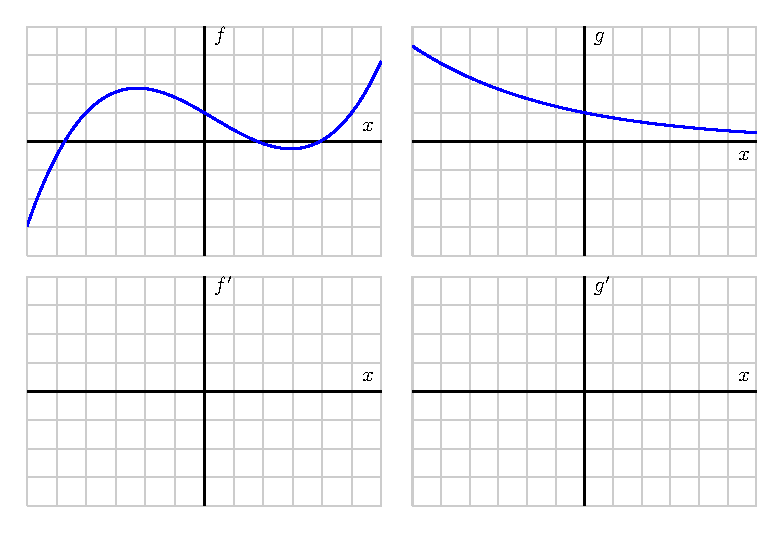
\includegraphics{figures/1_4_Act1a.eps} 
\centerline{\hspace{4in}}
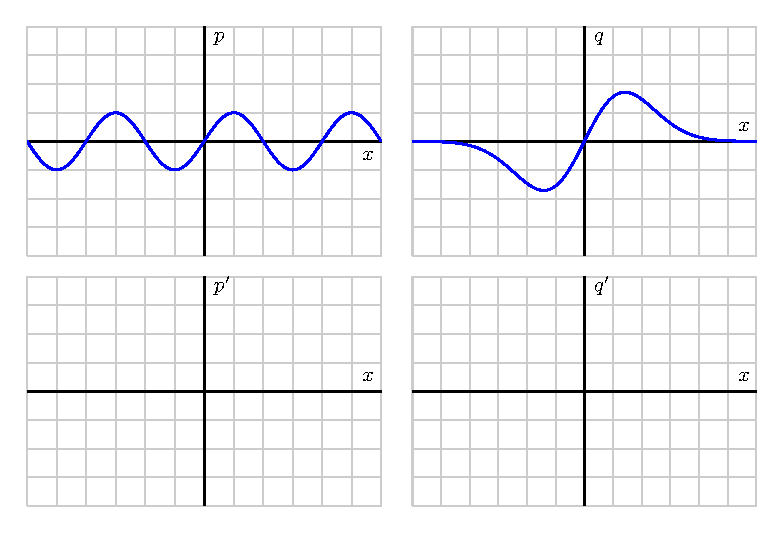
\includegraphics{figures/1_4_Act1b.eps}
\end{center}
\end{adjustwidth*}

\begin{center}
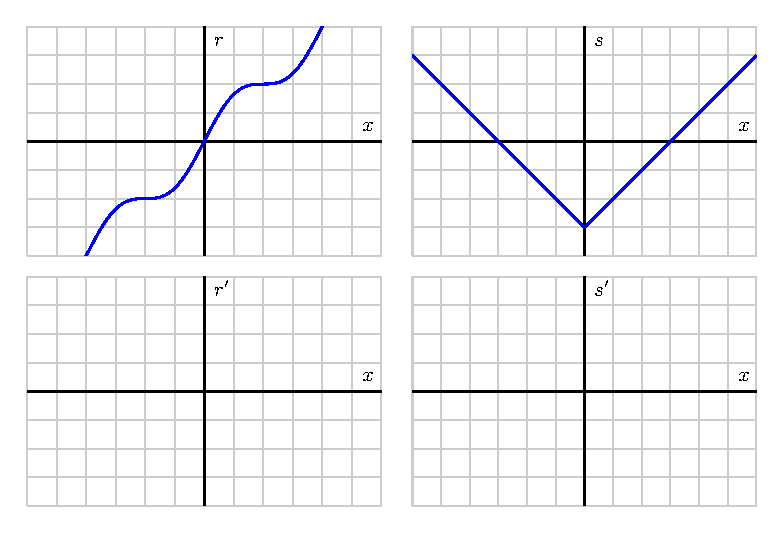
\includegraphics{figures/1_4_Act1c.eps}
\centerline{\hspace{4in}}
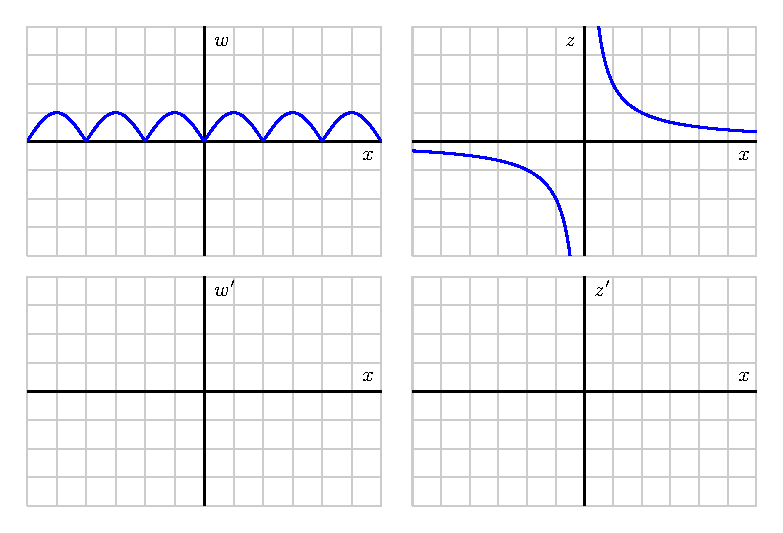
\includegraphics{figures/1_4_Act1d.eps}
\end{center}


\begin{smallhint}
Points where the slope of the tangent line is equal to zero are particularly important.  Try finding these points first in your effort to plot $y = f'(x)$ and plotting those zero values on the axes where you'll graph $y = f'(x)$.  
\end{smallhint}
\begin{bighint}
Points where the slope of the tangent line is equal to zero are particularly important.  Try finding these points first in your effort to plot $y = f'(x)$ and plotting those zero values on the axes where you'll graph $y = f'(x)$.  After doing so, think carefully as well about the questions: at this point, is $f'(x)$ positive or negative?  is $f'(x)$ big or small.  Use these ideas to help you sketch the derivative graph for the following functions.
\end{bighint}
\begin{activitySolution}
\begin{center}
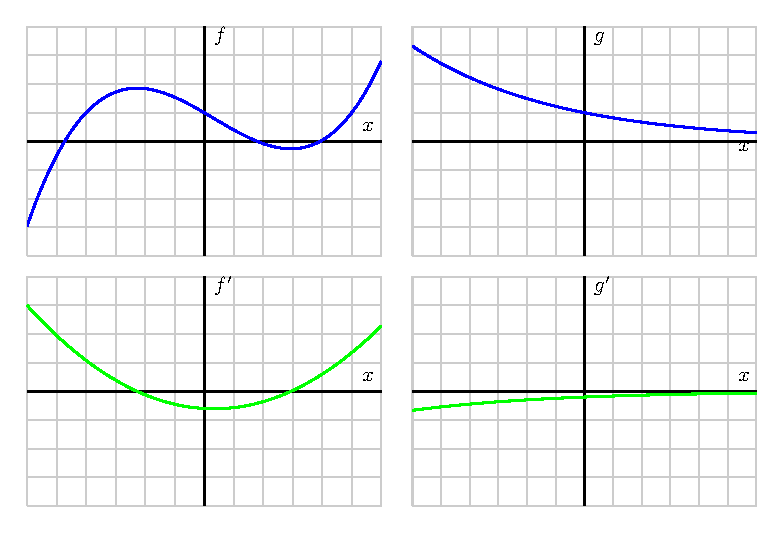
\includegraphics{figures/1_4_Act1aSoln.eps} \\
\underline{\hspace{4in}}\\
\ \\
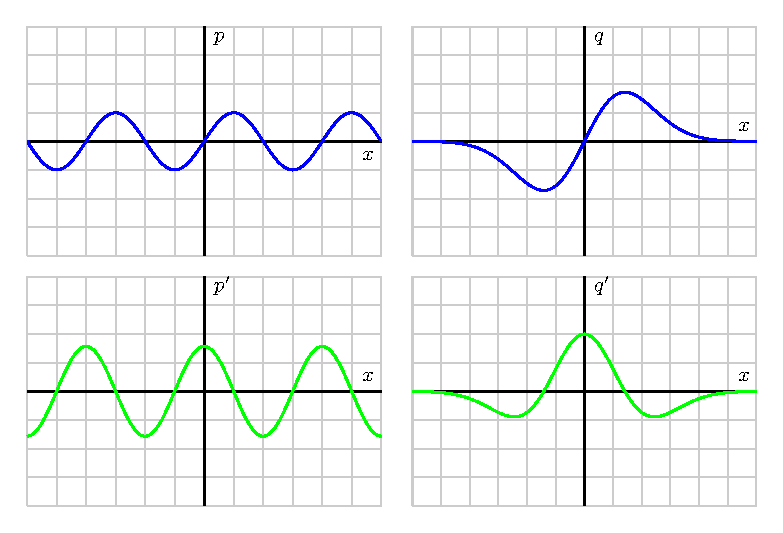
\includegraphics{figures/1_4_Act1bSoln.eps}
\end{center}

\begin{center}
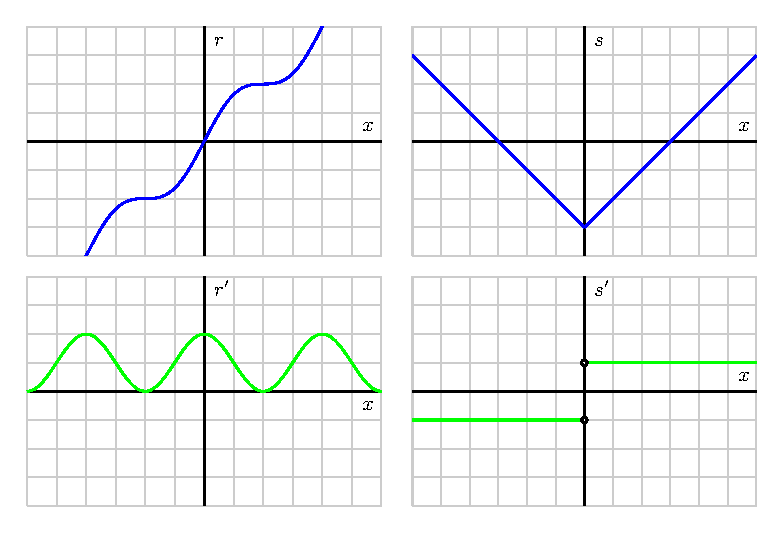
\includegraphics{figures/1_4_Act1cSoln.eps} \\
\underline{\hspace{4in}}\\
\ \\
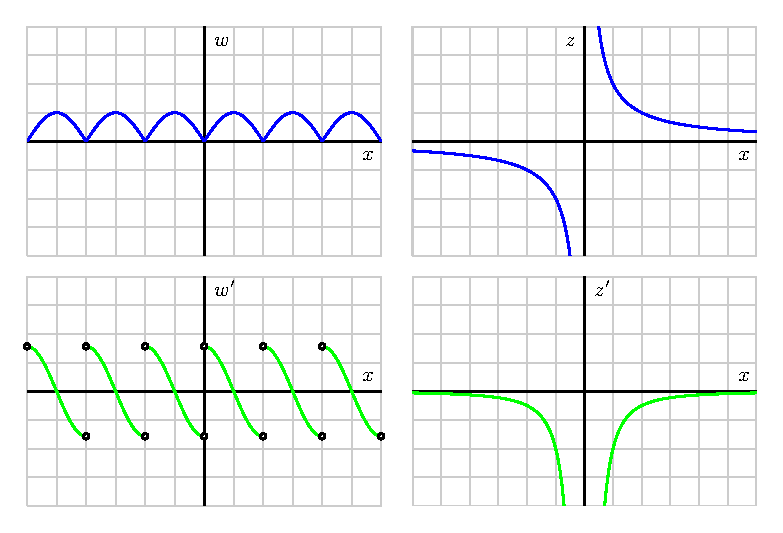
\includegraphics{figures/1_4_Act1dSoln.eps}
\end{center}
\end{activitySolution}
\aftera % ACTIVITY 

\marginnote{For a dynamic investigation that allows you to experiment with graphing $f'$ when given the graph of $f$, see \href{http://gvsu.edu/s/8y}{\texttt{http://gvsu.edu/s/8y}}.(Source: Marc Renault, Calculus Applets Using Geogebra.)} 

Now, recall the opening example of this section:  we began with the function $y = f(x) = 4x - x^2$ and used the limit definition of the derivative to show that $f'(a) = 4 - 2a$, or equivalently that $f'(x) = 4 - 2x$.  We subsequently graphed the functions $f$ and $f'$ as shown in Figure~\ref{fig:2-2_ffprime}.  Following Activity~\ref{A:2.2.1}, we now understand that we could have constructed a fairly accurate graph of $f'(x)$ \emph{without} knowing a formula for either $f$ or $f'$.  At the same time, it is ideal to know a formula for the derivative function whenever it is possible to find one.

\begin{example} \label{Ex:2.2.Eg1}
Let $f(x) = 3x^2+5x-7$. Find $f'(x)$.

\solution We apply the definition of the derivative.
\begin{align*}
f'(x) &= \lim_{h \to 0} \frac{f(x+h)-f(x)}{h} \\
&=	\lim_{h \to 0} \frac{3(x+h)^2+5(x+h)-7-(3x^2+5x-7)}{h}\\
&=	\lim_{h \to 0} \frac{3h^2 +6xh+5h}{h}\\
&= \lim_{h \to 0} 3h+6x+5 \\
&= 6x+5
\end{align*}
So $f'(x) = 6x+5$. Recall in Example~\ref{Ex:2.1.Eg2} of Section~\ref{S:2.1.DerivativePt}, we found that $f'(1) = 11$ and $f'(3) = 23$. Note our new computation of $f'(x)$ affirm these facts.
\end{example}

 % EXAMPLE

\begin{example} \label{Ex:2.2.Eg2}
Let $\ds f(x) = \frac{1}{x+1}$. Find $f'(x)$.

\solution We again apply the definition of the derivative.
\begin{align*}
f'(x) &= \lim_{h \to 0} \frac{f(x+h)-f(x)}{h}\\
&=	\lim_{h\to 0} \frac{\frac{1}{x+h+1}-\frac{1}{x+1}}{h} \intertext{Now find a common denominator then subtract; pull $1/h$ out front to facilitate reading.}
&= \lim_{h\to 0} \frac{1}{h}\cdot\left(\frac{x+1}{(x+1)(x+h+1)} - \frac{x+h+1}{(x+1)(x+h+1)}\right)\\
&=	\lim_{h\to 0} \frac 1h\cdot\left(\frac{x+1-(x+h+1)}{(x+1)(x+h+1)}\right)\\
&=	\lim_{h\to 0} \frac1h\cdot\left(\frac{-h}{(x+1)(x+h+1)}\right)\\
&=	\lim_{h\to 0} \frac{-1}{(x+1)(x+h+1)} \\
&= \frac{-1}{(x+1)(x+1)}\\
&= \frac{-1}{(x+1)^2}
\end{align*}
	
So $\ds f'(x) = \frac{-1}{(x+1)^2}$. To practice our notation, we could also state 
\[ \ds \frac{d}{dx}\left(\frac{1}{x+1}\right) = \frac{-1}{(x+1)^2}. \]
\end{example}

 %EXAMPLE

In the next activity, we further explore the more algebraic approach to finding $f'(x)$:  given a formula for $y = f(x)$, the limit definition of the derivative will be used to develop a formula for $f'(x)$.  

\begin{activity} \label{A:2.2.2}
For each of the listed functions, determine a formula for the derivative function.  For the first two, determine the formula for the derivative by thinking about the nature of the given function and its slope at various points; do not use the limit definition.  For the latter four, use the limit definition.  Pay careful attention to the function names and independent variables.  It is important to be comfortable with using letters other than $f$ and $x$.  For example, given a function $p(z)$, we call its derivative $p'(z)$.
\begin{multicols}{3}
\ba
	\item $\ds (x) = 1$
	\item $\ds g(t) = t$
	\item $\ds p(z) = z^2$
	\item $\ds q(s) = s^3$
	\item $\ds F(t) = \frac{1}{t}$
	\item $\ds G(y) = \sqrt{y}$
\ea
\end{multicols}

\end{activity}
\begin{smallhint}
\ba
	\item  What is the slope of the function at every point?
	\item  What is the slope of the function at every point?
	\item  $p(z+h) = (z+h)^2$
	\item  $q(s+h) = (s+h)^3$
	\item  $F(t+h) = \frac{1}{t+h}$
	\item  $G(y+h) = \sqrt{y+h}$
\ea
\end{smallhint}
\begin{bighint}
\ba
	\item  The function is a horizontal line.
	\item  The function is a line with slope 1.
	\item  $p(z+h) - p(z) = (z+h)^2 - z^2 = z^2 + 2zh + h^2 - z^2$
	\item  $q(s+h) - q(s) = (s+h)^3 - s^3 = s^3 + 3s^2h + 3sh^2 + h^3 - s^3$
	\item  Find a common denominator for $ \frac{1}{t+h} - \frac{1}{t}$.
	\item  Multiply the difference quotient by this form of 1: $\frac{\sqrt{y+h} + \sqrt{y}}{\sqrt{y+h} + \sqrt{y}}.$
\ea
\end{bighint}
\begin{activitySolution}
\ba
	\item  $f'(x) = 0$ because the slope of the tangent line to the horizontal line given by $f(x) = 1$ is zero at every value of $x$.
	\item  $g'(t) = 1$ because the slope of the tangent line to the line given by $g(t) = t$ is 1 at every value of $t$.
	\item  \begin{eqnarray*}
		p'(z) & = & \lim_{h \to 0} \frac{p(z+h) - p(z)}{h} \\
		       & = & \lim_{h \to 0} \frac{(z+h)^2 - z^2}{h} \\
		       & = & \lim_{h \to 0} \frac{z^2 + 2zh + h^2 - z^2}{h} \\
		       & = & \lim_{h \to 0} \frac{2zh + h^2}{h} \\
		       & = & \lim_{h \to 0} 2z + h \\
		       & = & 2z
		 \end{eqnarray*}
		 
	\item  \begin{eqnarray*}
		q'(s) & = & \lim_{h \to 0} \frac{q(s+h) - q(s)}{h} \\
		       & = & \lim_{h \to 0} \frac{(s+h)^3 - s^3}{h} \\
		       & = & \lim_{h \to 0} \frac{s^3 + 3s^2h + 3sh^2 + h^3 - s^3}{h} \\
		       & = & \lim_{h \to 0} \frac{3s^2h + 3sh^2 + h^2}{h} \\
		       & = & \lim_{h \to 0} 3s^2 + 3sh + h \\
		       & = & 3s^2
		 \end{eqnarray*}
	\item  \begin{eqnarray*}
		F'(t) & = & \lim_{h \to 0} \frac{F(t+h) - F(s)}{h} \\
		       & = & \lim_{h \to 0} \frac{\frac{1}{t+h} - \frac{1}{t}}{h} \\
		       & = & \lim_{h \to 0} \frac{\frac{t - (t+h)}{t(t+h)}}{h} \\
		       & = & \lim_{h \to 0} \frac{-h}{ht(t+h)} \\
		       & = & \lim_{h \to 0} \frac{-1}{t(t+h)} \\
		       & = & \frac{-1}{t^2}
		 \end{eqnarray*}
	\item  \begin{eqnarray*}
		G'(y) & = & \lim_{h \to 0} \frac{G(y+h) - G(y)}{h} \\
		       & = & \lim_{h \to 0} \frac{\sqrt{y+h}-\sqrt{y}}{h} \\
		       & = & \lim_{h \to 0} \frac{\sqrt{y+h}-\sqrt{y}}{h} \cdot \frac{\sqrt{y+h} + \sqrt{y}}{\sqrt{y+h} + \sqrt{y}} \\
		       & = & \lim_{h \to 0} \frac{(y+h)-y}{h(\sqrt{y+h} + \sqrt{y})} \\
		       & = & \lim_{h \to 0} \frac{h}{h(\sqrt{y+h} + \sqrt{y})} \\
		       & = & \lim_{h \to 0} \frac{1}{\sqrt{y+h} + \sqrt{y}} \\
		       & = & \frac{1}{2\sqrt{y}}
		 \end{eqnarray*}		 
\ea
\end{activitySolution}
\aftera % ACTIVITY 

%-------------------------------------------
% SUBSECTION DIFFERENTIABILITY
%-------------------------------------------
\subsection*{Differentiability}

We recall that a function $f$ is said to be differentiable at $x = a$ whenever $f'(a)$ exists.  Moreover, for $f'(a)$ to exist, we know that the function $y = f(x)$ must have a tangent line at the point $(a,f(a))$, since $f'(a)$ is precisely the slope of this line.  In order to even ask if $f$ has a tangent line at $(a,f(a))$, it is necessary that $f$ be continuous at $x = a$: if $f$ fails to have a limit at $x = a$, if $f(a)$ is not defined, or if $f(a)$ does not equal the value of $\ds \lim_{x \to a} f(x)$, then it doesn't even make sense to talk about a tangent line to the curve at this point.

Indeed, it can be proved formally that if a function $f$ is differentiable at $x = a$, then it must be continuous at $x = a$.  So, if $f$ is not continuous at $x = a$, then it is automatically the case that $f$ is not differentiable there.  For example, in Figure~\ref{fig:1-3_Con} from our early discussion of continuity, both $f$ and $g$ fail to be differentiable at $x = 1$ because neither function is continuous at $x = 1$.  But can a function fail to be differentiable at a point where the function is continuous?

In Figure~\ref{F:1.7.NotDiff}, we consider the situation where a function has a sharp corner at a point.  For the pictured function $f$, we observe that $f$ is clearly continuous at $a = 1$, since $\ds\lim_{x \to 1} f(x) = 1 = f(1).$

\begin{marginfigure} % MARGIN FIGURE
\margingraphics{figures/1_7_NotDiff.eps}
\caption{A function $f$ that is continuous at $a = 1$ but not differentiable at $a = 1$; at right, we zoom in on the point $(1,1)$ in a magnified version of the box in the left-hand plot.} \label{F:1.7.NotDiff}
\end{marginfigure}

But the function $f$ in Figure~\ref{F:1.7.NotDiff} is not differentiable at $a = 1$ because $f'(1)$ fails to exist.  One way to see this is to observe that $f'(x) = -1$ for every value of $x$ that is less than $1$, while $f'(x) = +1$ for every value of $x$ that is greater than $1$.  That makes it seem that either $+1$ or $-1$ would be equally good candidates for the value of the derivative at $x = 1$.   Alternately, we could use the limit definition of the derivative to attempt to compute $f'(1)$, and discover that the derivative does not exist.  Finally, we can also see visually that the function $f$ in Figure~\ref{F:1.7.NotDiff} does not have a tangent line.  When we zoom in on $(1,1)$ on the graph of $f$, no matter how closely we examine the function, it will always look like a ``V'', and never like a single line, which tells us there is no possibility for a tangent line there.  

To make a more general observation, if a function does have a tangent line at a given point, when we zoom in on the point of tangency, the function and the tangent line should appear essentially indistinguishable\footnote{See, for instance, \href{http://gvsu.edu/s/6J}{\texttt{http://gvsu.edu/s/6J}} for an applet (due to David Austin, GVSU) where zooming in shows the increasing similarity between the tangent line and the curve.  }.  Conversely, if we have a function such that when we zoom in on a point the function looks like a single straight line, then the function should have a tangent line there, and thus be differentiable.  Hence, a function that is differentiable at $x = a$ will, up close, look more and more like its tangent line at $(a,f(a))$, and thus we say that a function is differentiable at $x = a$ is \emph{locally linear}. \index{locally linear}

\begin{marginfigure}[1.5cm] % MARGIN FIGURE
\captionsetup[subfigure]{labelformat=empty}
\subfloat{\margingraphics{figures/figabsolutevalue}}

\subfloat{\margingraphics{figures/figabsolutevalueprime}}
\caption{Above: The absolute value function, $f(x) = |x|$. Notice how the slope of the lines (and hence the tangent lines) abruptly changes at $x=0$. Below: A graph of the derivative of $f(x) = |x|$.}\label{fig:2-2_Eg3.1}
\end{marginfigure}

\begin{example} \label{Ex:2.2.Eg3}
Find the derivative of the absolute value function---see Figure~\ref{fig:2-2_Eg3.1}.
\[ f(x) = |x| = \left\{\begin{array}{cc} -x & x<0 \\ x & x\geq 0\end{array}.\right. \]

\solution We need to evaluate $\ds \lim_{h \to 0}\frac{f(x+h)-f(x)}{h}.$ As $f$ is piecewise--defined, we need to consider separately the limits when $x<0$ and when $x>0$. 

When $x<0$:
\begin{align*}
\frac{d}{dx}\big(-x\big) 	&= \lim_{h\to 0}\frac{-(x+h) - (-x)}{h} \\
&=	\lim_{h \to 0}\frac{-h}{h}\\
&=	\lim_{h \to 0}-1 \\
&=	-1.
\end{align*}
When $x>0$, a similar computation shows that $\ds \frac{d}{dx}\big( x \big) = 1$. \\

We need to also find the derivative at $x=0$. By the definition of the derivative at a point, we have 
\[ f'(0) = \lim_{h \to 0}\frac{f(0+h)-f(0)}{h}.\]
Since $x=0$ is the point where our function's definition switches from one piece to other, we need to consider left and right-hand limits. Consider the following, where we compute the left and right hand limits side by side.

\noindent\begin{minipage}[b]{.5\linewidth}
\begin{align*}
\lim_{h \to 0^-} \frac{f(0+h)-f(0)}{h} &= \\
\lim_{h \to 0^-} \frac{-h-0}{h} &= \\
\lim_{h \to 0^-} -1 & =-1
\end{align*}
\end{minipage}\rule{.5pt}{70pt}
\begin{minipage}[b]{.5\linewidth}
\begin{align*}
\lim_{h \to 0^+} \frac{f(0+h)-f(0)}{h} &= \\
\lim_{h \to 0^+} \frac{h-0}{h} &= \\
\lim_{h \to 0^+} 1 & =1
\end{align*}
\end{minipage}
%		
%		$$\begin{array}{ccccc}
%		\displaystyle \lim_{h\to0}\frac{f(0+h)-f(0)}{h} & = & \displaystyle\lim_{h\to0^-}\frac{f(0+h)-f(0)}{h} &=&\displaystyle\lim_{h\to0^+}\frac{f(0+h)-f(0)}{h}\\
%	\rule{0pt}{20pt}	&= & \displaystyle\lim_{h\to0^-}\frac{-h-0}{h} &=&\displaystyle\lim_{h\to0^+}\frac{h-0}{h}\\
%	\rule{0pt}{15pt}	&= & \displaystyle\lim_{h\to0^-}-1 &=&\displaystyle\lim_{h\to0^+}1\\
%	\rule{0pt}{12pt}	&= & -1 &=& 1\ !\\
%		\end{array}$$
%		
		
The last lines of each column tell the story: the left and right hand limits are not equal. Therefore the limit does not exist at $0$, and $f$ is not differentiable at $0$.
So we have 
\[ f'(x) = \left\{\begin{array}{cc} -1 & x<0 \\ 1 & x>0\end{array}.\right.\] 
At $x=0$, $f'(x)$ does not exist; there is a jump discontinuity at $0$; see Figure~\ref{fig:2-2_Eg3.1}. So $f(x) = |x|$ is differentiable everywhere except at $0$. 
\end{example}

 %EXAMPLE

\begin{marginfigure}[6cm]
\margingraphics{figures/1_7_PA1.eps}
\caption{The graph of $y = f(x)$ for Activity~\ref{A:2.2.3}.} \label{fig:2.2.Act3}
\end{marginfigure}

\begin{activity} \label{A:2.2.3} 
In this activity, we classify the points at which a function does not have a limit and is neither continuous nor differentiable.  Let $f$ be the function given in Figure~\ref{fig:2.2.Act3}.
\ba
\item State all values of $a$ for which $f$ does not have a limit at $x = a$.  For each, provide a reason for your conclusion.
\item State all values of $a$ for which $f$ is not continuous at $x = a$.  For each, provide a reason for your conclusion.
\item State all values of $a$ for which $f$ is not differentiable at $x = a$.  For each, provide a reason for your conclusion.
\item True or false: if a function $p$ is differentiable at $x = b$, then $\ds \lim_{x \to b} p(x)$ must exist.  Why?	
\ea

\end{activity}
\begin{smallhint}
\ba
	\item What type of function is $g$ for all $x < 0$?  For all $x > 0$?
	\item Recall that $g'(0) = \lim_{h \to 0} \frac{g(0 + h) - g(0)}{h}.$
	\item What is the value of $|h|$ when $h < 0$?
	\item You might start by identifying points where $f$ is not continuous.
	\item What does being differentiable at a point tell you about continuity there?	
\ea
\end{smallhint}
\begin{bighint}
\ba
	\item Think about how $g$ is a piecewise linear function.
	\item Recall that $g'(0) = \lim_{h \to 0} \frac{g(0 + h) - g(0)}{h}.$
	\item What is the value of $|h|$ when $h < 0$?  What does this tell you about $\frac{|h|}{h}$ when $h < 0$?
	\item Start by identifying points where $f$ is not continuous.  Then strive to identify any corner points.
	\item What does being differentiable at a point tell you about continuity at that point?	
\ea
\end{bighint}
\begin{activitySolution}
\ba
	\item We know that $g(x) = |x|$ is given by the formula $g(x) = -x$ when $x < 0$ and by $g(x) = x$ when $x \ge 0$.  Each of these pieces of $g$ is a straight line, so at every point other than the point where they meet, the function $g$ has a well-defined slope, and thus is differentiable. 
	\item Observe that
	\begin{eqnarray*}
		g'(0) & = & \lim_{h \to 0} \frac{g(0+h)-g(0)}{h} \\
			& = & \lim_{h \to 0} \frac{|0+h|-|0|}{h} \\
			& = & \lim_{h \to 0} \frac{|h|}{h}
	\end{eqnarray*}
	\item Following up on our work in (b), note that whenever $h > 0$, $|h| = h$, and thus
	$$\lim_{h \to 0^+} \frac{|h|}{h} = \lim_{h \to 0^+} \frac{h}{h} = 1,$$
	while whenever $h < 0$, $|h| = -h$, and thus
	$$\lim_{h \to 0^-} \frac{|h|}{h} = \lim_{h \to 0^-} \frac{-h}{h} = -1$$
	Since the right- and left-hand limits are not equal, it follows that 
	$$g'(0) =  \lim_{h \to 0} \frac{|h|}{h}$$
	does not exist.

	\item $f$ is not differentiable at $a = -2, -1, 2, 3$ because at each of these points $f$ is not continuous.  In addition, $f$ is not differentiable at $a = -3$ and $a = 1$ because the graph of $f$ has a corner point (or cusp) at each of these values.  
	\item True: if a function $p$ is differentiable at $x = b$, then $\lim_{x \to b} p(x)$ must exist.  This is true because we know that if $p$ is differentiable at a point, then $p$ is continuous there, and anytime a function is continuous at a point, it must have a limit there.	
\ea
\end{activitySolution}
\aftera % ACTIVITY This needs to now be redone!!

%--------------
% SUMMARY
%--------------
\begin{summary}
\item The limit definition of the derivative, $f'(x) = \lim_{h \to 0} \frac{f(x+h)-f(x)}{h}$, produces a value for each $x$ at which the derivative is defined, and this leads to a new function whose formula is $y = f'(x)$.  Hence we talk both about a given function $f$ and its derivative $f'$.  

\item There is essentially no difference between writing $f'(a)$ (as we did regularly in Section~\ref{S:2.1.DerivativePt}) and writing $f'(x)$.  In either case, the variable is just a placeholder that is used to define the rule for the derivative function.

\item Given the graph of a function $y = f(x)$, we can sketch an approximate graph of its derivative $y = f'(x)$ by observing that \emph{heights} on the derivative's graph correspond to \emph{slopes} on the original function's graph.

\item In this section, we encountered some functions that had sharp corners on their graphs, such as the shifted absolute value function.  At such points, the derivative fails to exist, and we say that $f$ is not differentiable there.  For now, it suffices to understand this as a consequence of the jump that must occur in the derivative function at a sharp corner on the graph of the original function.  
\end{summary}

%--------------
% EXERCISES
%--------------
\begin{adjustwidth*}{}{-2.25in}
\textbf{{\large Exercises}}
\setlength{\columnsep}{25pt}
\begin{multicols*}{2}
\noindent Terms and Concepts \small
\begin{enumerate}[1)]
\item {T/F: Let $f$ be a position function. The average rate of change on $[a,b]$ is the slope of the line through the points $(a, f(a))$ and $(b,f(b))$.}
\item {T/F: The definition of the derivative of a function at a point involves taking a limit.}
\item {In your own words, explain the difference between the average rate of change and instantaneous rate of change.}
\item Let $y = f(x)$. Give three different notations equivalent to ``$f'(x)$.''
\end{enumerate} 

\noindent {\normalsize Problems} \small

\noindent {\bf In exercises 5--8, a graph of a function is given. Using the graph, sketch $f'(x)$.}

\begin{enumerate}[1),resume]
\item 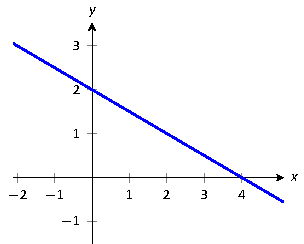
\includegraphics[scale=.8]{figures/fig02_01_ex_26}
\item 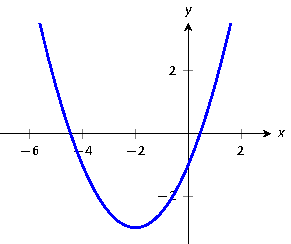
\includegraphics[scale=.8]{figures/fig02_01_ex_27}
\item 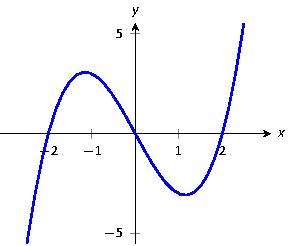
\includegraphics[scale=.8]{figures/fig02_01_ex_28}
\item \includegraphics[scale=.8]{figures/fig02_01_ex_29}

\item Using the graph of $g(x)$ below, answer the following questions.
\ba
\item Where is $g(x) > 0$?
\item Where is $g(x) < 0$?
\item Where is $g(x) = 0$?
\item Where is $g'(x) < 0$?
\item Where is $g'(x) > 0$?
\item Where is $g'(x) = 0$?
\ea

\includegraphics[scale=.8]{figures/fig02_01_ex_30}

\item Let $f$ be a function with the following properties:  $f$ is differentiable at every value of $x$ (that is, $f$ has a derivative at every point), $f(-2) = 1$, and $f'(-2) = -2$, $f'(-1) = -1$, $f'(0) = 0$, $f'(1) = 1$, and $f'(2) = 2$.
\ba
	\item On the axes provided at left below, sketch a possible graph of $y = f(x)$.  Explain why your graph meets the stated criteria.
	\item On the axes at right below, sketch a possible graph of $y = f'(x)$.  What type of curve does the provided data suggest for the graph of $y = f'(x)$?
	\item Conjecture a formula for the function $y = f(x)$.  Use the limit definition of the derivative to determine the corresponding formula for $y = f'(x)$.  Discuss both graphical and algebraic evidence for whether or not your conjecture is correct.
\ea

\includegraphics[scale=.75]{figures/1_2_Ez3.eps} 
\end{enumerate}

%------------------------------------------
% END OF EXERCISES ON FIRST PAGE
%------------------------------------------
\end{multicols*}
\end{adjustwidth*}

\clearpage

\begin{adjustwidth*}{}{-2.25in}
\setlength{\columnsep}{25pt}
\begin{multicols*}{2}\small

\begin{enumerate}[1),start=11]
\item Let $g$ be a continuous function (that is, one with no jumps or holes in the graph) and suppose that a graph of $y= g'(x)$ is given by the graph on the right below.

\includegraphics[scale=.75]{figures/1_4_Ez2.eps} %\ \  \includegraphics{figures/1_2_Ez3.eps}

\ba
\item Observe that for every value of $x$ that satisfies $0 < x < 2$, the value of $g'(x)$ is constant.  What does this tell you about the behavior of the graph of $y = g(x)$ on this interval?
\item On what intervals other than $0 < x < 2$ do you expect $y = g(x)$ to be a linear function?  Why?
\item At which values of $x$ is $g'(x)$ not defined?  What behavior does this lead you to expect to see in the graph of $y=g(x)$?
\item Suppose that $g(0) = 1$.  On the axes provided at left, sketch an accurate graph of $y = g(x)$.
\ea

\item Consider the graph of the function $y = p(x)$ that is provided below on the left.  Assume that each portion of the graph of $p$ is a straight line, as pictured.

\includegraphics[scale=.75]{figures/1_7_Ez2.eps}

\ba
\item State all values of $a$ for which $\lim_{x \to a} p(x)$ does not exist.
\item State all values of $a$ for which $p$ is not continuous at $a$.
\item State all values of $a$ for which $p$ is not differentiable at $x = a$.
\item On the axes provided on the right, sketch an accurate graph of $y = p'(x)$.
\ea

\item For each of the following prompts, give an example of a function that satisfies the stated criteria.  A formula or a graph, with reasoning, is sufficient for each.  If no such example is possible, explain why.
\ba
\item A function $f$ that is continuous at $a = 2$ but not differentiable at $a = 2$.
\item A function $g$ that is differentiable at $a = 3$ but does not have a limit at $a=3$.
\item A function $h$ that has a limit at $a = -2$, is defined at $a = -2$, but is not continuous at $a = -2$.
\item A function $p$ that satisfies all of the following:
\begin{itemize}
\item $p(-1) = 3$ and $\ds\lim_{x \to -1} p(x) = 2$
\item $p(0) = 1$ and $p'(0) = 0$
\item $\ds\lim_{x \to 1} p(x) = p(1)$ and $p'(1)$ does not exist
\end{itemize}
\ea
\end{enumerate}

\vspace{.25cm}

\noindent {\bf For exercises 14--22, use the limit definition of the derivative to compute the derivative function.}

\bmtwo
\begin{enumerate}[1),resume]
\item $\ds f(x) = 8x$
\item $\ds y = x^2$
\item $\ds g(x) = 2x^2 + 3x$
\item $\ds s(t) = \frac{1}{\ds \sqrt{t}}$
\item $\ds r(x) = \frac{1}{x^2}$
\item $\ds f(x) = \ds\sqrt{3x-1}$
\item $\ds f(x) = \ds\sqrt{8x}$
\item $\ds s(t) = \frac{1}{t + 5}$
\item $\ds y = \frac{1}{2x - 1}$
\end{enumerate}
\emtwo

%------------------------------------------------
% END OF EXERCISES ON SECOND PAGE
%------------------------------------------------
\end{multicols*}
\end{adjustwidth*}
\afterexercises 

\cleardoublepage
\section{The second derivative} \label{S:2.3.SecondD}

\begin{goals}
\item How does the derivative of a function tell us whether the function is increasing or decreasing at a point or on an interval?
\item What can we learn by taking the derivative of the derivative (to achieve the \emph{second} derivative) of a function $f$?
\item What does it mean to say that a function is concave up or concave down?  How are these characteristics connected to certain properties of the derivative of the function?
\item What are the units on the second derivative?  How do they help us understand the rate of change of the rate of change?
\end{goals}

%--------------------------------------
% SUBSECTION INTRODUCTION
%--------------------------------------
\subsection*{Introduction}

\begin{marginfigure}[8cm] % MARGIN FIGURE
\margingraphics{figures/1_6_Intro.eps} %ACTIVE 1.25
\caption{Two tangent lines on a graph demonstrate how the slope of the tangent line tells us whether the function is rising or falling, as well as whether it is doing so rapidly or slowly.}\label{fig:2-3_Intro}
\end{marginfigure}

Given a differentiable function $y= f(x)$, we know that its derivative, $y = f'(x)$, is a related function whose output at a value $x=a$ tells us the slope of the tangent line to $y = f(x)$ at the point $(a,f(a))$.  That is, heights on the derivative graph tell us the values of slopes on the original function's graph.  Therefore, the derivative tells us important information about the function $f$.  

At any point where $f'(x)$ is positive, it means that the slope of the tangent line to $f$ is positive, and therefore the function $f$ is increasing (or rising) \index{increasing} at that point.  Similarly, if $f'(a)$ is negative, we know that the graph of $f$ is decreasing \index{decreasing} (or falling) at that point.   

In the next part of our study, we work to understand not only \emph{whether} the function $f$ is increasing or decreasing at a point or on an interval, but also \emph{how} the function $f$ is increasing or decreasing.  Comparing the two tangent lines shown in Figure~\ref{fig:2-3_Intro}, we see that at point $A$, the value of $f'(x)$ is positive and relatively close to zero, which coincides with the graph rising slowly.  By contrast, at point $B$, the derivative is negative and relatively large in absolute value, which is tied to the fact that $f$ is decreasing rapidly at $B$.  It also makes sense to not only ask whether the value of the derivative function is positive or negative and whether the derivative is large or small, but also to ask "how is the derivative changing?"

We also now know that the derivative, $y = f'(x)$, is itself a function.  This means that we can consider taking its derivative -- the derivative of the derivative -- and therefore ask questions like "what does the derivative of the derivative tell us about how the original function behaves?"  As we have done regularly in our work to date, we start with an investigation of a familiar problem in the context of a moving object.  

\begin{marginfigure}[1cm]
\margingraphics{figures/1_6_PA1.eps}
\caption{The graph of $y = s(t)$, the position of the car (measured in thousands of feet from its starting location) at time $t$ in minutes.} \label{fig:2.3.PA1}
\end{marginfigure}

\begin{pa} \label{PA:2.3}
The position of a car driving along a straight road at time $t$ in minutes is given by the function $y = s(t)$ that is pictured in Figure~\ref{fig:2.3.PA1}.  The car's position function has units measured in thousands of feet.  For instance, the point $(2,4)$ on the graph indicates that after $2$ minutes, the car has traveled $4000$ feet.

\ba
	\item In everyday language, describe the behavior of the car over the provided time interval.  In particular, you should carefully discuss what is happening on each of the time intervals $[0,1]$, $[1,2]$, $[2,3]$, $[3,4]$, and $[4,5]$, plus provide commentary overall on what the car is doing on the interval $[0,12]$.
	\item On the lefthand axes provided in Figure~\ref{fig:2.3.PA1b}, sketch a careful, accurate graph of $y = s'(t)$.
	\item What is the meaning of the function $y = s'(t)$ in the context of the given problem?  What can we say about the car's behavior when $s'(t)$ is positive?  when $s'(t)$ is zero?  when $s'(t)$ is negative?
	\item Rename the function you graphed in (b) to be called $y = v(t)$.  Describe the behavior of $v$ in words, using phrases like ``$v$ is increasing on the interval $\ldots$'' and ``$v$ is constant on the interval $\ldots$.''
	\item Sketch a graph of the function $y = v'(t)$ on the righthand axes provide in Figure~\ref{fig:2.3.PA1b}.  Write at least one sentence to explain how the behavior of $v'(t)$ is connected to the graph of $y=v(t)$.
\ea

\end{pa} 

\begin{figure}
\includegraphics{figures/1_6_PA1b.eps}
\caption{Axes for plotting $y = v(t) = s'(t)$ and $y = v'(t)$.} \label{fig:2.3.PA1b}
\end{figure}

\afterpa

 % PREVIEW ACTIVITY

%-----------------------------------
% SUBSECTION INCREASE,DECREASE
%-----------------------------------
\subsection*{Increasing, decreasing, or neither}

When we look at the graph of a function, there are features that strike us naturally, and common language can be used to name these features.  In many different settings so far, we have intuitively used the words \emph{increasing} and \emph{decreasing} to describe a function's graph.  Here we connect these terms more formally to a function's behavior on an interval of input values.

\definition{Increasing/Decreasing}{% DEFINITION
Given a function $f(x)$ defined on the interval $(a,b)$, we say that \emph{$f$ is increasing on $(a,b)$} provided that for all $x$, $y$ in the interval $(a,b)$, if $x < y$, then $f(x) < f(y)$.  Similarly, we say that \emph{$f$ is decreasing on $(a,b)$} provided that for all $x$, $y$ in the interval $(a,b)$, if $x < y$, then $f(x) > f(y)$.
} % end definition

Simply put, an increasing function is one that is rising as we move from left to right along the graph, and a decreasing function is one that falls as the value of the input increases.  For a function that has a derivative at a point, we will also talk about whether or not the function is increasing or decreasing \emph{at that point}.  Moreover, the fact of whether or not the function is increasing, decreasing, or neither at a given point depends precisely on the value of the derivative at that point.

\concept{Increasing/Decreasing at a Point}{% CONCEPT
Let $f$ be a function that is differentiable at $x = a$.  Then $f$ is increasing at $x = a$ if and only if $f'(a) > 0$ and $f$ is decreasing at $x = a$ if and only if $f'(a) < 0$.  If $f'(a) = 0$, then we say $f$ is neither increasing nor decreasing at $x = a$.
} % end concept

\begin{marginfigure}[1cm] % MARGIN FIGURE
\margingraphics{figures/1_6_Intro2.eps} %ACTIVE 1.28
\caption{A function that is decreasing at $A$, increasing at $B$, and more generally, decreasing on the intervals $-3 < x < -2$ and $0 < x  < 2$ and increasing on $-2 < x < 0$ and $2 < x < 3$.} \label{fig:2.3.Intro2}
\end{marginfigure}

For example, the function pictured in Figure~\ref{fig:2.3.Intro2} is increasing at any point at which $f'(x)$ is positive, and hence is increasing on the entire interval $-2 < x < 0$.  Note that at both $x = \pm 2$ and $x = 0$, we say that $f$ is neither increasing nor decreasing, because $f'(x) = 0$ at these values.

\begin{example} \label{Ex:2.3.Eg1}
Let $f(x) = x^3+x^2-x+1$. Find intervals on which $f$ is increasing or decreasing.

\solution We first find the values where $f$ is neither increasing or decreasing. Given $f'(x) = 3x^2+2x-1 = (3x-1)(x+1)$, then  $f'(x) = 0$ when $x=-1$ and when $x=1/3$. Notice that $f'$ is never undefined.

Since an interval was not specified for us to consider, we consider the entire domain of $f$, which is $(-\infty,\infty)$. We thus break the whole real line into three subintervals based on the two values where the derivative is zero: $(-\infty,-1)$, $(-1,1/3)$ and $(1/3,\infty)$. This is shown in Figure \ref{F:2.3.Eg1-1}.

We now pick a value $p$ in each subinterval and find the sign of $f'(p)$. All we care about is the sign, so we do not actually have to fully compute $f'(p)$; pick "nice" values that make this simple.

\noindent\textbf{Subinterval 1}, $(-\infty,-1)$:\quad We (arbitrarily) pick $p=-2$. We can compute $f'(-2)$ directly: $f'(-2) = 3(-2)^2+2(-2)-1=7>0$. We conclude that $f$ is increasing on $(-\infty,-1)$.

Note we can arrive at the same conclusion without computation. For instance, we could choose $p=-100$. The first term in $f'(-100)$, i.e., $3(-100)^2$ is clearly positive and very large. The other terms are small in comparison, so we know $f'(-100)>0$. All we need is the sign.\\

\noindent\textbf{Subinterval 2}, $(-1,1/3)$:\quad We pick $p=0$ since that value seems easy to deal with. $f'(0) = -1<0$. We conclude $f$ is decreasing on $(-1,1/3)$.\\

\noindent\textbf{Subinterval 3}, $(1/3,\infty)$:\quad Pick an arbitrarily large value for $p>1/3$ and note that $f'(p) =3p^2+2p-1 >0$. We conclude that $f$ is increasing on $(1/3,\infty)$.

We can verify our calculations by considering Figure \ref{F:2.3.Eg1-2}, where $f$ is graphed in blue. The graph also presents $f'$ in red; note how $f'>0$ when $f$ is increasing and $f'<0$ when $f$ is decreasing.
\end{example}

\begin{marginfigure}[-15cm]
\margingraphics{figures/figincrline1} %APEX EX 84 
\caption{Number line for $f$ in Example \ref{Ex:2.3.Eg1}.}\label{F:2.3.Eg1-1}
\end{marginfigure}

\begin{marginfigure}[-6cm]
\margingraphics{figures/figincr1} %APEX EX 84
\caption{A graph of $f(x)$ in Example \ref{Ex:2.3.Eg1}, showing where $f$ is increasing and decreasing.}\label{F:2.3.Eg1-2}
\end{marginfigure} %EXAMPLE

%-----------------------------------
% SUBSECTION SECOND DERIVATIVE
%-----------------------------------
\subsection*{The Second Derivative} \index{second derivative}

For any function, we are now accustomed to investigating its behavior by thinking about its derivative.  Given a function $f$, its derivative is a new function, one that is given by the rule
\[ f'(x) = \lim_{h \to 0} \frac{f(x+h)-f(x)}{h}. \]
Because $f'$ is itself a function, it is perfectly feasible for us to consider the derivative of the derivative, which is the new function $y = [f'(x)]'$.  We call this resulting function \emph{the second derivative}\index{second derivative} of $y = f(x)$, and denote the second derivative by $y = f''(x)$.
Due to the presence of multiple possible derivatives, we will sometimes call $f'$ ``the first derivative'' of $f$, rather than simply ``the derivative'' of $f$. Formally, the second derivative is defined by the limit definition of the derivative of the first derivative:
\[ f''(x) = \lim_{h \to 0} \frac{f'(x+h)-f'(x)}{h}. \]

We note that all of the established meaning of the derivative function still holds, so when we compute $y = f''(x)$, this new function measures slopes of tangent lines to the curve $y = f'(x)$, as well as the instantaneous rate of change of $y = f'(x)$.  In other words, just as the first derivative measures the rate at which the original function changes, the second derivative measures the rate at which the first derivative changes.  This means that the second derivative tracks the instantaneous rate of change of the instantaneous rate of change of $f$.  That is, the second derivative will help us to understand how the rate of change of the original function is itself changing.

%-----------------------------------
% SUBSECTION CONCAVITY
%-----------------------------------
\subsection*{Concavity}

In addition to asking \emph{whether} a function is increasing or decreasing, it is also natural to inquire \emph{how} a function is increasing or decreasing.  To begin, there are three basic behaviors that an increasing function can demonstrate on an interval, as pictured in Figure~\ref{fig:2.3optsi}:  the function can increase more and more rapidly, increase at the same rate, or increase in a way that is slowing down.  Fundamentally, we are beginning to think about how a particular curve bends, with the natural comparison being made to lines, which don't bend at all.  More than this, we want to understand how the bend in a function's graph is tied to behavior characterized by the first derivative of the function.

\begin{figure*} % FIGURE
\begin{flushleft}
\captionsetup[subfigure]{labelformat=empty}
\subfloat{\includegraphics[scale=.5]{figs/2/2-3_Cona.pdf}}
\subfloat{\includegraphics[scale=.5]{figs/2/2-3_Conb.pdf}}
\subfloat{\includegraphics[scale=.5]{figs/2/2-3_Conc.pdf}}
\caption{Three functions that are all increasing, but doing so at an increasing rate, at a constant rate, and at a decreasing rate, respectively.}\label{fig:2.3optsi}
\end{flushleft}
\end{figure*}

For the leftmost curve in Figure~\ref{fig:2.3optsi}, picture a sequence of tangent lines to the curve.  As we move from left to right, the slopes of those tangent lines will increase.  Therefore, the rate of change of the pictured function is increasing, and this explains why we say this function is \emph{increasing at an increasing rate}.  For the rightmost graph in Figure~\ref{fig:2.3optsi}, observe that as $x$ increases, the function increases but the slope of the tangent line decreases, hence this function is \emph{increasing at a decreasing rate}.

Of course, similar options hold for how a function can decrease.  Here we must be extra careful with our language, since decreasing functions involve negative slopes, and negative numbers present an interesting situation in the tension between common language and mathematical language.  For example, it can be tempting to say that ``$-100$ is bigger than $-2$.''  But we must remember that when we say one number is greater than another, this describes how the numbers lie on a number line:  $x < y$ provided that $x$ lies to the left of $y$.  So of course, $-100$ is less than $-2$.  Informally, it might be helpful to say that ``$-100$ is more negative than $-2$.''  This leads us to note particularly that when a function's values are negative, and those values subsequently get more negative, the function must be decreasing.

Now consider the three graphs shown in Figure~\ref{fig:2.3optsd}.  Clearly the middle graph demonstrates the behavior of a function decreasing at a constant rate.  If we think about a sequence of tangent lines to the first curve that progress from left to right, we see that the slopes of these lines get less and less negative as we move from left to right.  That means that the values of the first derivative, while all negative, are increasing, and thus we say that the leftmost curve is \emph{decreasing at an increasing rate}.

\begin{figure*}[h] % FIGURE
\begin{flushright}
\captionsetup[subfigure]{labelformat=empty}
\subfloat{\includegraphics[scale=.5]{figs/2/2-3_Cond.pdf}}
\subfloat{\includegraphics[scale=.5]{figs/2/2-3_Cone.pdf}}
\subfloat{\includegraphics[scale=.5]{figs/2/2-3_Conf.pdf}}
\caption{From left to right, three functions that are all decreasing, but doing so in different ways.}\label{fig:2.3optsd}
\end{flushright}
\end{figure*}

This leaves only the rightmost curve in Figure~\ref{fig:2.3optsd} to consider.  For that function, the slope of the tangent line is negative throughout the pictured interval, but as we move from left to right, the slopes get more and more negative.  Hence the slope of the curve is decreasing, and we say that the function is \emph{decreasing at a decreasing rate}.

This leads us to introduce the notion of \emph{concavity} \index{concavity} which provides simpler language to describe some of these behaviors.  Informally, when a curve opens up on a given interval, like the upright parabola $y = x^2$ or the exponential growth function $y = e^x$, we say that the curve is \emph{concave up} on that interval.  Likewise, when a curve opens down, such as the parabola $y = -x^2$ or the opposite of the exponential function $y = -e^{x}$, we say that the function is \emph{concave down}.  This behavior is linked to both the first and second derivatives of the function.  

\begin{marginfigure}[0cm] % MARGIN FIGURE
\margingraphics{figures/1_6_concavity.eps}
\caption{At left, a function that is concave up; at right, one that is concave down.}\label{fig:2-3_concavity}
\end{marginfigure}

In Figure~\ref{fig:2-3_concavity}, we see two functions along with a sequence of tangent lines to each.  On the lefthand plot where the function is concave up, observe that the tangent lines to the curve always lie below the curve itself and that, as we move from left to right, the slope of the tangent line is increasing.  Said differently, the function $f$ is concave up on the interval shown because its derivative, $f'$, is increasing on that interval.  Similarly, on the righthand plot in Figure~\ref{fig:2-3_concavity}, where the function shown is concave down, there we see that the tangent lines alway lie above the curve and that the value of the slope of the tangent line is decreasing as we move from left to right.  Hence, what makes $f$ concave down on the interval is the fact that its derivative, $f'$, is decreasing.

We state these most recent observations formally as the definitions of the terms \emph{concave up} and \emph{concave down}.

\definition{Concave Up/Down} % DEFINITION
{Let $f$ be a differentiable function on an interval $(a,b)$.  Then $f$ is \emph{concave up} \index{concave up} on $(a,b)$ if and only if $f'$ is increasing on $(a,b)$;  $f$ is \emph{concave down} \index{concave down} on $(a,b)$ if and only if $f'$ is decreasing on $(a,b)$.
} % end definition

\begin{marginfigure}[6cm]
\margingraphics{figures/figconcline1} %APEX EX 87
\caption{A number line determining the concavity of $f$ in Example \ref{Ex:2.3.Eg2}.}\label{F:2.3.Eg2-1}
\end{marginfigure}

\begin{marginfigure}[1cm]
\margingraphics{figures/figconc1} %APEX EX 87
\caption{A graph of $f(x)$ used in Example \ref{Ex:2.3.Eg2}.}\label{F:2.3.Eg2-2}
\end{marginfigure}

\begin{example} \label{Ex:2.3.Eg2}
Let $f(x)=x^3-3x+1$. Find the intervals on which $f$ is concave up/down.

\solution We first find the values where $f$ is neither increasing or decreasing.  Given $f'(x)=3x^2-3$ and $f''(x)=6x$, then $f''(x) = 0$ only when $x=0$. Notice that $f''$ is never undefined.

Since an interval was not specified for us to consider, we consider the entire domain of $f$, which is $(-\infty,\infty)$. We use a process similar to the one used in Example~\ref{Ex:2.3.Eg1} to determine the intervals where $f$ is increasing/decreasing. Thus break the whole real line into two subintervals based on the value where the second derivative is zero: $(-\infty,0)$ and $(0,\infty)$. \\

\noindent\textbf{Subinterval 1}, $(-\infty,0)$:\quad Picking any value $c<0$, we can easily see that $f''(c)<0$; so $f$ is concave down on $(-\infty,0)$. \\

\noindent\textbf{Subinterval 2}, $(0, \infty)$:\quad  Picking any value $c>0$, we can easily see that $f''(c)>0$; so $f$ is concave up on $(0,\infty)$. \\

The number line in Figure \ref{F:2.3.Eg2-1} illustrates the process of determining concavity; Figure \ref{F:2.3.Eg2-1} shows a graph of $f$ in blue and $f''(x)$ in red, confirming our results. Notice how $f$ is concave down precisely when $f''(x)<0$ and concave up when $f''(x)>0$.
\end{example} % EXAMPLE

The following activities lead us to further explore how the first and second derivatives of a function determine the behavior and shape of its graph.  We begin by revisiting Preview Activity~\ref{PA:2.3}.

\begin{activity} \label{A:2.3.1}
The position of a car driving along a straight road at time $t$ in minutes is given by the function $y = s(t)$ that is pictured in Figure~\ref{fig:2.3.A1}.  The car's position function has units measured in thousands of feet.  Remember that you worked with this function and sketched graphs of $y = v(t) = s'(t)$ and $y = v'(t)$ in Preview Activity~\ref{PA:2.3}.

\ba
\item On what intervals is the position function $y = s(t)$ increasing? decreasing?  Why?
\item On which intervals is the velocity function $y = v(t) = s'(t)$ increasing? decreasing? neither?  Why?
\item \emph{Acceleration} \index{acceleration} is defined to be the instantaneous rate of change of velocity, as the acceleration of an object measures the rate at which the velocity of the object is changing.  Say that the car's acceleration function is named $a(t)$.  How is $a(t)$ computed from $v(t)$?  How is $a(t)$ computed from $s(t)$?  Explain.
\item What can you say about $s''$ whenever $s'$ is increasing?  Why?
\item Using only the words \emph{increasing}, \emph{decreasing}, \emph{constant}, \emph{concave up}, \emph{concave down}, and \emph{linear}, complete the following sentences.  For the position function $s$ with velocity $v$ and acceleration $a$,
	\begin{itemize}
		\item on an interval where $v$ is positive, $s$ is \underline{\hspace{1.5in}}.
		\item on an interval where $v$ is negative, $s$ is \underline{\hspace{1.5in}}. 
		\item on an interval where $v$ is zero, $s$ is \underline{\hspace{1.5in}}.

		\item on an interval where $a$ is positive, $v$ is \underline{\hspace{1.5in}}.
		\item on an interval where $a$ is negative, $v$ is \underline{\hspace{1.5in}}. 
		\item on an interval where $a$ is zero, $v$ is \underline{\hspace{1.5in}}.

		\item on an interval where $a$ is positive, $s$ is \underline{\hspace{1.5in}}.
		\item on an interval where $a$ is negative, $s$ is \underline{\hspace{1.5in}}. 
		\item on an interval where $a$ is zero, $s$ is \underline{\hspace{1.5in}}.
	\end{itemize}
\ea

\end{activity}

\begin{marginfigure}[-18cm]
\includegraphics{figures/1_6_PA1.eps}
\caption{The graph of $y = s(t)$, the position of the car (measured in thousands of feet from its starting location) at time $t$ in minutes.} \label{fig:2.3.A1}
\end{marginfigure}


\begin{smallhint}
\ba
	\item Remember that a function is increasing on an interval if and only if its first derivative is positive on the interval.
	\item See (a).
	\item Remember that the first derivative of a function measures its instantaneous rate of change.
	\item Think about how $s''(t) = [s'(t)]'$.
	\item Be very careful with your letters:  $s$, $v$, and $a$. 
\ea
\end{smallhint}
\begin{bighint}
\ba
	\item Remember that a function is increasing on an interval if and only if its first derivative is positive on the interval and that $v(t) = s'(t)$.
	\item See (a), and note that $v'(t) = s''(t)$.
	\item Remember that the first derivative of a function measures its instantaneous rate of change, so $s''(t)$ measures the instantaneous rate of change of $v(t) = s'(t)$.
	\item Note that $s''(t) = [s'(t)]'$, so $s''(t)$ is the slope of the tangent line to $y = s'(t)$.
	\item Be very careful with your letters:  $s$, $v$, and $a$.  For instance, note that when acceleration is positive, velocity must be increasing.
\ea
\end{bighint}
\begin{activitySolution}
\ba
	\item The position function $y = s(t)$ increasing on the intervals $0<t<2$, $3<t<5$, $7<t<9$, and $10<t<12$, because at every point in such intervals, $s'(t)$ is positive.  For the provided function, $s(t)$ is never decreasing because its derivative is never negative.
	\item The velocity function $y = v(t)$ appears to be increasing on the intervals $0<t<1$, $3<t<4$, $7<t<8$, and $10<t<11$ because the curve $y = s(t)$ is concave up which corresponds to an increasing first derivative $y =s'(t)$.  Similarly, $y = v(t)$ appears to be decreasing on the intervals $1<t<2$, $4<t<5$, $8<t<9$, and $11<t<12$ because the curve $y = s(t)$ is concave down which corresponds to a decreasing first derivative $y =s'(t)$.  On the intervals $2<t<3$, $5<t<7$, and $9<t<10$, the curve $y = s(t)$ is constant, and thus linear, so neither concave up nor concave down.  
	\item Since $a(t)$ is the instantaneous rate of change of $v(t)$, $a(t) = v'(t)$.  And because $v(t) = s'(t)$, it follows that $a(t) = v'(t) = [s'(t)]' = s''(t)$, so acceleration is the second derivative of position. 
	\item Because $s''(t)$ is the first derivative of $s'(t)$, when $s'(t)$ is increasing, $s''(t)$ must be positive.
	\item For the position function $s(t)$ with velocity $v(t)$ and acceleration $a(t)$,
	\begin{itemize}
		\item on an interval where $v(t)$ is positive, $s(t)$ is \underline{increasing}.
		\item on an interval where $v(t)$ is negative, $s(t)$ is \underline{decreasing}. 
		\item on an interval where $v(t)$ is zero, $s(t)$ is \underline{constant}.

		\item on an interval where $a(t)$ is positive, $v(t)$ is \underline{increasing}.
		\item on an interval where $a(t)$ is negative, $v(t)$ is \underline{decreasing}. 
		\item on an interval where $a(t)$ is zero, $v(t)$ is \underline{constant}.

		\item on an interval where $a(t)$ is positive, $s(t)$ is \underline{concave up}.
		\item on an interval where $a(t)$ is negative, $s(t)$ is \underline{concave down}. 
		\item on an interval where $a(t)$ is zero, $s(t)$ is \underline{linear}.
	\end{itemize}
\ea
\end{activitySolution}
\aftera %ACTIVITY

The context of position, velocity, and acceleration is an excellent one in which to understand how a function, its first derivative, and its second derivative are related to one another.  In Activity~\ref{A:2.3.1}, we can replace $s$, $v$, and $a$ with an arbitrary function $f$ and its derivatives $f'$ and $f''$, and essentially all the same observations hold.  In particular, note that $f'$ is increasing if and only if $f$ is concave up, and similarly $f'$ is increasing if and only if $f''$ is positive.  Likewise, $f'$ is decreasing if and only if $f$ is concave down, and $f'$ is decreasing if and only if $f''$ is negative.

\newpage

\vspace*{-.75cm}

\begin{margintable}[1cm]
\begin{center}
\scalebox{1.25}{
\begin{tabular}{cc}
\begin{tabular}{| l || l |}
\hline
$t$ & $F(t)$ \\ \hline \hline
$0$ & $70$ \\ \hline
$15$ & $180.5$ \\ \hline
$30$ & $251$ \\ \hline
$45$ & $296$ \\ \hline
$60$ & $324.5$ \\ \hline
$75$ & $342.8$ \\ \hline
$90$ & $354.5$  \\ \hline
\end{tabular}
&
\begin{tabular}{| l || l |}
\hline
$t$ & $F'(t)$ \\ \hline \hline
$0$ & NA\\ \hline
$15$ & $6.03$ \\ \hline
$30$ & $3.85$ \\ \hline
$45$ & $2.45$ \\ \hline
$60$ & $1.56$ \\ \hline
$75$ & $1.00$ \\ \hline
$90$ & NA  \\ \hline
\end{tabular}
\end{tabular}

} % end scalebox
\end{center}
\caption{The temperatures and rates of change of the temperature of a potato in an oven.}\label{T:2-3_Act2}
\end{margintable}

\begin{activity} \label{A:2.3.3}
A potato is placed in an oven, and the potato's temperature $F$ (in degrees Fahrenheit) at various points in time is taken and recorded in Table~\ref{T:2-3_Act2}. Time $t$ is measured in minutes.  In Activity~\ref{A:2.1.5}, we computed approximations to $F'(30)$ and $F'(60)$ using central differences.  Those values and more are also provided in Table~\ref{T:2-3_Act2}, along with several others computed in the same way.

\ba
	\item What are the units on the values of $F'(t)$? 
	\item Use a central difference to estimate the value of $F''(30)$.
	\item What is the meaning of the value of $F''(30)$ that you have computed in (b) in terms of the potato's temperature?  Write several careful sentences that discuss, with appropriate units, the values of $F(30)$, $F'(30)$, and $F''(30)$, and explain the overall behavior of the potato's temperature at this point in time.
	\item Overall, is the potato's temperature increasing at an increasing rate, increasing at a constant rate, or increasing at a decreasing rate?  Why?
\ea

\end{activity}
\begin{smallhint}
\ba
	\item Remember that the derivative's units are ``units of output per unit of input.'' 
	\item To estimate $g'(a)$, we can use 
	$$g'(a) \approx \frac{g(a+h)-g(a-h)}{2h}$$
	for an appropriate choice of $h$.
	\item For each of the values $F'(30)$ and $F''(30)$, think about what they tell you about expected upcoming behavior in $F(t)$ and $F'(t)$, respectively.
	\item Think concavity.
\ea
\end{smallhint}
\begin{bighint}
\ba
	\item Remember that the derivative's units are ``units of output per unit of input.'' 
	\item To estimate $g'(a)$, we can use 
	$$g'(a) \approx \frac{g(a+h)-g(a-h)}{2h}$$
	for an appropriate choice of $h$.  So, observe that
	$$F''(a) \approx \frac{F'(a+h)-F'(a-h)}{2h}$$
	\item For each of the values $F'(30)$ and $F''(30)$, think about what they tell you about expected upcoming behavior in $F(t)$ and $F'(t)$, respectively.  What do you expect to be the values of $F(31)$ and $F'(31)$?  Why?
	\item Examine the given data and think about how the graph of $y = F(t)$ will appear.
\ea
\end{bighint}
\begin{activitySolution}
\ba
	\item $F'(t)$ has units measured in degrees Fahrenheit per minute. 
	\item Using a central difference, 
	$$F''(30) \approx \frac{F'(45)-F'(15)}{30} = \frac{2.45-6.03}{30} \approx -0.119.$$
	\item The value $F''(30) \approx -0.119$, which is measured in degrees per minute per minute tells us, along with the other data, that at the moment $t = 30$, the temperature of the potato is 251 degrees, that its temperature is rising at a rate of 3.85 degrees per minute, and that the rate at which the temperature is rising is \emph{falling} at a rate of -0.119 degrees per minute per minute.  That is, while the temperature is rising, it is rising at a slower and slower rate.  At $t = 31$, we'd expect that the rate of increase of the potato's temperature would have dropped to about 3.73 degrees per minute.
	\item The potato's temperature increasing at a decreasing rate because the values of the first derivative of $F$ are falling.  Equivalently, this is because the value of $F''(t)$ is negative throughout the given time interval.
\ea
\end{activitySolution}
\aftera %ACTIVITY

%\begin{figure}

%\caption{Two given functions $f$, with axes provided for plotting $f'$ and $f''$ below.} \label{F:1.6.A2}
%\end{figure}


\begin{activity} \label{A:2.3.2}
This activity builds on our experience and understanding of how to sketch the graph of $f'$ given the graph of $f$.  Below, given the graph of a function $f$, sketch $f'$ and then sketch $f''$.  In addition, for each, write several careful sentences in the spirit of those in Activity~\ref{A:2.3.1} that connect the behaviors of $f$, $f'$, and $f''$.  For instance, write something such as
\begin{quote}
``$f'$ is \underline{\hspace{1.5in}} on the interval \underline{\hspace{0.5in}}, which is connected to the fact that $f$ is \underline{\hspace{1.5in}} on the same interval \underline{\hspace{0.5in}}, and $f''$ is \underline{\hspace{1.5in}} on the interval as well...''
\end{quote}
but of course with the blanks filled in.  Throughout, view the scale of the grid for the graph of $f$ as being $1 \times 1$, and assume the horizontal scale of the grid for the graph of $f'$ is identical to that for $f$.  If you need to adjust the vertical scale on the axes for the graph of $f'$ or $f''$, you should label that accordingly.
\end{activity}

%\begin{adjustwidth*}{}{-.85in}
%\begin{center}
%\includegraphics{figures/1_4_Act1a.eps} 
%\centerline{\hspace{4in}}
%\includegraphics{figures/1_4_Act1b.eps}
%\end{center}
%\end{adjustwidth*}

\begin{adjustwidth*}{}{-1.5in}
\includegraphics[scale=.5]{figs/2/2-3_Act2a.pdf}
\includegraphics[scale=.5]{figs/2/2-3_Act2b.pdf}
\end{adjustwidth*}

\begin{smallhint}
Remember that to plot $y = f'(x)$, it is helpful to first identify where $f'(x) = 0.$
\end{smallhint}
\begin{bighint}
Remember that to plot $y = f'(x)$, it is helpful to first identify where $f'(x) = 0$, and then ask where $y = f'(x)$ is positive and negative.  In a similar way, once $y = f'(x)$ has been plotted, to construct the graph of $y=f''(x)$, it is useful to note where the slope of the tangent line to $y = f'(x)$ is zero, as well as where such slopes are positive and negative.  Heights on the graph of $y = f''(x)$ will correspond to slopes on $y = f'(x)$.
\end{bighint}
\begin{activitySolution}
The graphs of $f'$ and $f''$ are plotted in Figure~***.
%%%%HMMM
%\begin{figure}[h]
%\begin{center}
%\includegraphics{figures/1_6_Act2Soln.eps}
%\caption{Two given functions $f$, with axes provided for plotting $f'$ and $f''$ below.} \label{F:1.6.A2Soln}
%\end{center}
%\end{figure}
%plus commentary after updating the figure
\end{activitySolution}
\aftera %ACTIVITY

%---------------------------------------------
% SUBSECTION HIGHER DERIVATIVES
%---------------------------------------------
\subsection*{Higher Derivatives}
So far in this section we have discussed how the derivative of a function $f$ is itself a function, therefore we can take its derivative. We can repeat this process as long as the corresponding limits exist. The following concept introduces the notation we use for higher derivatives. 

\concept{Higher Order Derivatives}{ % CONCEPT
Let $y=f(x)$ be a differentiable function on $I$. \index{derivative!higher order} \index{derivative!notation}
\begin{enumerate}[1)]
\item The \textit{second derivative} of $f$ is: 
	\[ f''(x) = \frac{d}{dx}\Big( f'(x) \Big) = \frac{d}{dx} \left( \frac{dy}{dx} \right) = \frac{d^2y}{dx^2}=y''. \]
\item The \textit{third derivative} of $f$ is: 
	\[ f'''(x) = \frac{d}{dx} \Big( f''(x) \Big) = \frac{d}{dx} \left( \frac{d^2y}{dx^2} \right) = \frac{d^3y}{dx^3}=y'''.\]
\item The \textit{n$^{\text{th}}$ derivative} of $f$ is:
	\[ f^{(n)}(x) = \frac{d}{dx} \left( f^{(n-1)}(x) \right) = \frac{d}{dx} \left( \frac{d^{n-1}y}{dx^{n-1}} \right) = \frac{d^ny}{dx^n}=y^{(n)}. \]
\end{enumerate}
} % end concept

In general, when finding the fourth derivative and on, we resort to the $f^{(4)}(x)$ notation, not $f''''(x)$; after a while, too many ticks is too confusing. Let's practice using this new concept.

\begin{example} \label{Ex:2.3.Eg3}
Find the first four derivatives of $f(x) = 4x^2$.

\solution Using the limit definition of the derivative, we compute the first derivative as
\begin{align*}
f'(x) & = \lim_{h \to 0} \frac{f(x+h) - f(x)}{h} \\
& = \lim_{h \to 0} \frac{4(x+h)^2 - 4x^2}{h} = \lim_{h \to 0} \frac{4(x^2 + 2xh + h^2) - 4x^2}{h} \\
&= \lim_{h \to 0} \frac{4x^2 + 8xh + 4h^2 - 4x^2}{h} = \lim_{h \to 0} \frac{8xh + 4h^2}{h} \\
&= \lim_{h \to 0} \frac{h(8x + 4h)}{h} = \lim_{h \to 0} 8x + 4h = 8x.
\end{align*}

We compute the second derivative as
\begin{align*}
f''(x) &= \lim_{h \to 0} \frac{f'(x+h) - f'(x)}{h} \\
&= \lim_{h \to 0} \frac{8(x+h) - 8x}{h} = \lim_{h \to 0} \frac{8x + 8h - 8x}{h} \\
&= \lim_{h \to 0} \frac{8h}{h} = \lim_{h \to 0} 8 = 8.
\end{align*}

We compute the third derivative as
\begin{align*}
f'''(x) &= \lim_{h \to 0} \frac{f''(x+h) - f''(x)}{h} \\
&= \lim_{h \to 0} \frac{8 - 8}{h} = \lim_{h \to 0} \frac{0}{h} = 0.
\end{align*}

We compute the fourth derivative as
\begin{align*}
f^{(4)}(x) &= \lim_{h \to 0} \frac{f'''(x+h) - f'''(x)}{h} \\
&= \lim_{h \to 0} \frac{0 - 0}{h} = \lim_{h \to 0} \frac{0}{h} = 0.
\end{align*}

\end{example} %EXAMPLE

It can be difficult to consider the meaning of the third, and higher order, derivatives. The third derivative is "the rate of change of the rate of change of the rate of change of $f$." That is essentially meaningless to the uninitiated. In the context of our position/velocity/acceleration example, the third derivative is the "rate of change of acceleration," commonly referred to as "jerk." 

Make no mistake: higher order derivatives have great importance even if their practical interpretations are hard (or "impossible") to understand. The mathematical topic of \textit{series} makes extensive use of higher order derivatives.

\begin{summary}
\item A differentiable function $f$ is increasing at a point or on an interval whenever its first derivative is positive, and decreasing whenever its first derivative is negative.
\item By taking the derivative of the derivative of a function $f$, we arrive at the second derivative, $f''$.  The second derivative measures the instantaneous rate of change of the first derivative, and thus the sign of the second derivative tells us whether or not the slope of the tangent line to $f$ is increasing or decreasing.
\item A differentiable function is concave up whenever its first derivative is increasing (or equivalently whenever its second derivative is positive), and concave down whenever its first derivative is decreasing (or equivalently whenever its second derivative is negative).  %Examples of functions that are everywhere concave up are $y = x^2$ and $y = e^x$; examples of functions that are everywhere concave down are $y = -x^2$ and $y = -e^x$.
\item The units on the second derivative are "units of output per unit of input per unit of input."  They tell us how the value of the derivative function is changing in response to changes in the input.  In other words, the second derivative tells us the rate of change of the rate of change of the original function.
\end{summary}

%--------------
% EXERCISES
%--------------
\begin{adjustwidth*}{}{-2.25in}
\textbf{{\large Exercises}}
\setlength{\columnsep}{25pt}
\begin{multicols*}{2}
\noindent Terms and Concepts \small
\begin{enumerate}[1)]
\item Explain in  your own words what the second derivative ``means.''
\item If $f(x)$ describes a position function, then $f'(x)$ describes what kind of function? What kind of function is $f''(x)$?
\item Let $f(x)$ be a function measured in pounds, where $x$ is measured in feet. What are the units of $f''(x)$?
\item Explain in your own words how to find the third derivative of a function $f(x)$.
\end{enumerate} 

\noindent {\normalsize Problems} \small

%\noindent {\bf In exercises 5--8, a graph of a function is given. Using the graph, sketch $f'(x)$.}

\begin{enumerate}[1),resume]
\item Suppose that $y = f(x)$ is a differentiable function for which the following information is known:  $f(2) = -3$, $f'(2) = 1.5$, $f''(2) = -0.25$.
\ba
	\item Is $f$ increasing or decreasing at $x = 2$?  Is $f$ concave up or concave down at $x = 2$?
	\item Do you expect $f(2.1)$ to be greater than $-3$, equal to $-3$, or less than $-3$?  Why?
	\item Do you expect $f'(2.1)$ to be greater than $1.5$, equal to $1.5$, or less than $1.5$?  Why?
	\item Sketch a graph of $y = f(x)$ near $(2,f(2))$ and include a graph of the tangent line.  
\ea

\item For a certain function $y = g(x)$, its derivative is given by the function pictured below.
\begin{center}
\includegraphics[scale=.75]{figures/1_6_Ez2.eps}
\end{center}
\ba
	\item What is the approximate slope of the tangent line to $y = g(x)$ at the point $(2,g(2))$?
	\item How many real number solutions can there be to the equation $g(x) = 0$?  Justify your conclusion fully and carefully by explaining what you know about how the graph of $g$ must behave based on the given graph of $g'$.
	\item On the interval $-3 < x < 3$, how many times does the concavity of $g$ change?  Why?
	\item Use the provided graph to estimate the value of $g''(2)$.
\ea

\item For each prompt that follows, sketch a possible graph of a function on the interval $-3 < x < 3$ that satisfies the stated properties.
\ba
	\item $y = f(x)$ such that $f$ is increasing on $-3 < x < 3$, $f$ is concave up on $-3 < x < 0$, and $f$ is concave down on $0 < x < 3$.
	\item $y = g(x)$ such that $g$ is increasing on $-3 < x < 3$, $g$ is concave down on $-3 < x < 0$, and $g$ is concave up on $0 < x < 3$.
	\item $y = h(x)$ such that $h$ is decreasing on $-3 < x < 3$, $h$ is concave up on $-3 < x < -1$, neither concave up nor concave down on $-1 < x < 1$, and $h$ is concave down on $1 < x < 3$.
	\item $y = p(x)$ such that $p$ is decreasing and concave down on $-3 < x < 0$ and $p$ is increasing and concave down on $0 < x < 3$.
\ea

\item A bungee jumper's height $h$ (in feet ) at time $t$ (in seconds) is given in the table below.
\ba
	\item Use the given data to estimate $h'(4.5)$, $h'(5)$, and $h'(5.5)$.  At which of these times is the bungee jumper rising most rapidly?
	\item Use the given data and your work in (a) to estimate $h''(5)$.
	\item What physical property of the bungee jumper does the value of $h''(5)$ measure?  What are its units?
	\item Based on the data, on what approximate time intervals is the function $y = h(t)$ concave down?  What is happening to the velocity of the bungee jumper on these time intervals?
\ea

\begin{center}
\begin{tabular}{ccc}
\begin{tabular}{| l | l |} \hline
$t$ & $h(t)$ \\ \hline \hline
$0.0$ & $200$ \\ \hline
$0.5$ & $184.2$ \\ \hline
$1.0$ & $159.9$ \\ \hline
$1.5$ & $131.9$ \\ \hline
$2.0$ & $104.7$ \\ \hline
$2.5$ & $81.8$ \\ \hline
$3.0$ & $65.5$ \\ \hline
$3.5$ & $56.8$ \\ \hline
$4.0$ & $55.5$ \\ \hline
$4.5$ & $60.4$ \\ \hline
$5.0$ & $69.8$ \\ \hline
\end{tabular}
& &
\begin{tabular}{| l | l |} \hline
$t$ & $h(t)$ \\ \hline \hline
$5.5$ & $81.6$ \\ \hline
$6.0$ & $93.7$ \\ \hline
$6.5$ & $104.4$ \\ \hline
$7.0$ & $112.6$ \\ \hline
$7.5$ & $117.7$ \\ \hline
$8.0$ & $119.4$ \\ \hline
$8.5$ & $118.2$ \\ \hline
$9.0$ & $114.8$ \\ \hline
$9.5$ & $110.0$ \\ \hline
$10.0$ & $104.7$ \\ \hline
\end{tabular}
\end{tabular}
\end{center}

\end{enumerate}

%------------------------------------------
% END OF EXERCISES ON FIRST PAGE
%------------------------------------------
\end{multicols*}
\end{adjustwidth*}

\afterexercises 

\cleardoublepage
\section{Basic derivative rules} \label{S:2.4.BasicRules}

\begin{goals}
\item What are alternate notations for the derivative?
\item How can we sometimes use the algebraic structure of a function $f(x)$ to easily compute a formula for $f'(x)$?
\item What is the derivative of a power function of the form $f(x) = x^n$?  What is the derivative of an exponential function of form $f(x) = a^x$?
\item If we know the derivative of $y = f(x)$, how is the derivative of $y = k f(x)$ computed, where $k$ is a constant?
\item If we know the derivatives of $y = f(x)$ and $y = g(x)$, how is the derivative of $y = f(x) + g(x)$ computed?
\item What do the graphs of $y = \sin(x)$ and $y = \cos(x)$ suggest as formulas for their respective derivatives?
\end{goals}

%-----------------------------------
% SUBSECTION INTRODUCTION
%-----------------------------------
\subsection*{Introduction}

So far in this chapter, we developed the concept of the derivative of a function.  We now know that the derivative $f'$ of a function $f$ measures the instantaneous rate of change of $f$ with respect to $x$ as well as the slope of the tangent line to $y=f(x)$ at any given value of $x$.  To date, we have focused primarily on interpreting the derivative graphically or, in the context of functions in a physical setting, as a meaningful rate of change.  To actually calculate the value of the derivative at a specific point, we have typically relied on the limit definition of the derivative.

In this section, we will investigate how the limit definition of the derivative
\[ f'(x) = \lim_{h \to 0} \frac{f(x+h)-f(x)}{h} \]
leads to interesting patterns and rules that enable us to quickly find a formula for $f'(x)$ based on the formula for $f(x)$ \emph{without} using the limit definition directly.  For example, we already know that if $f(x) = x$, then it follows that $f'(x) = 1$.  While we could use the limit definition of the derivative to confirm this, we know it to be true because $f(x)$ is a linear function with slope $1$ at every value of $x$.  One of our goals is to be able to take standard functions, say ones such as $g(x) = 4x^7 - \sin(x) + 3e^x$, and, based on the algebraic form of the function, be able to apply shortcuts to almost immediately determine the formula for $g'(x)$.

\begin{pa} \label{PA:2.4}
Functions of the form $f(x) = x^n$, where $n = 1, 2, 3, \ldots$, are often called \emph{power functions}.  The first two questions below revisit work we did earlier, and the following questions extend those ideas to higher powers of $x$.
\ba
	\item Use the limit definition of the derivative to find $f'(x)$ for $f(x) = x^2$.
	\item Use the limit definition of the derivative to find $f'(x)$ for $f(x) = x^3$.
	\item Use the limit definition of the derivative to find $f'(x)$ for $f(x) = x^4$.  (Hint: $(a+b)^4 = a^4 + 4a^3b + 6a^2b^2 + 4ab^3 + b^4$.  Apply this rule to $(x+h)^4$ within the limit definition.)
	\item Based on your work in (a), (b), and (c), what do you conjecture is the derivative of $f(x) = x^5$?  Of $f(x) = x^{13}$?
	\item Conjecture a formula for the derivative of $f(x) = x^n$ that holds for any positive integer $n$.  That is, given $f(x) = x^n$ where $n$ is a positive integer, what do you think is the formula for $f'(x)$? 
\ea
\end{pa} \afterpa % PREVIEW ACTIVITY

%------------------------------------------
% SUBSECTION SOME KEY NOTATION
%------------------------------------------
%\subsection*{Some Key Notation}

%In addition to our usual $f'$ notation for the derivative, there are other ways to symbolically denote the derivative of a function, as well as the instruction to take the derivative.  We know that if we have a function, say  $f(x) = x^2$, that we can denote its derivative by $f'(x)$, and we write $f'(x) = 2x$.  Equivalently, if we are thinking more about the relationship between $y$ and $x$, we sometimes denote the derivative of $y$ with respect to $x$ with the symbol 
%$$\frac{dy}{dx}$$
%which we read ``dee-y dee-x.''  This notation comes from the fact that the derivative is related to the slope of a line, and slope is measured by $\frac{\triangle y}{\triangle x}$.  Note that while we read $\frac{\triangle y}{\triangle x}$ as ``change in $y$ over change in $x$,'' for the derivative symbol $\frac{dy}{dx}$, we view this is a single symbol, not a quotient of two quantities\footnote{That is, we do \emph{not} say ``dee-y over dee-x.''}.  For example, if $y = x^2$, we'll write that the derivative is $\frac{dy}{dx} = 2x.$

%Furthermore, we use a variant of $\frac{dy}{dx}$ notation to convey the instruction to take the derivative of a certain quantity with respect to a given variable.  In particular, if we write
%$$\frac{d}{dx}\left[ \Box \right]$$
%this means ``take the derivative of the quantity in $\Box$ with respect to $x$.''  To continue our example above with the squaring function, here we may write $\frac{d}{dx}[x^2] = 2x.$

%It is important to note that the independent variable can be different from $x$.  If we have $f(z) = z^2$, we then write $f'(z) = 2z$.  Similarly, if $y = t^2$, we can say $\frac{dy}{dt} = 2t$.  And changing the variable and derivative notation once more, it is also true that $\frac{d}{dq}[q^2] = 2q$.  This notation may also be applied to second derivatives:  $f''(z) =  \frac{d}{dz}\left[\frac{df}{dz}\right] = \frac{d^2 f}{dz^2}$.

%In what follows, we'll be working to widely expand our repertoire of functions for which we can quickly compute the corresponding derivative formula

%-----------------------------------------------------------------------------
% SUBSECTION CONSTANT, POWER, AND EXPONENTIAL FUNCTIONS
%-----------------------------------------------------------------------------
\subsection*{Constant, Power, and Exponential Functions}

So far, we have worked with the derivative formula for two important classes of functions:  constant functions and power functions.  For the first kind, observe that if $f(x) = c$ is a constant function, then its graph is a horizontal line with slope zero at every point.  Thus, $\frac{d}{dx}[c] = 0$.  We summarize this with the following rule.

\concept{Constant Rule \index{derivative!constant function}}{ % CONCEPT
For any real number $c$, if $f(x) = c$, then 
\[ f'(x) = 0. \]
} % end concept
Thus, if $f(x) = 7$, then $f'(x) = 0$.  Similarly, $\frac{d}{dx} [\sqrt{3}] = 0.$ 

\marginnote{The proof of the Constant Rule is found by applying the definition of the derivative, see Exercise~\ref{E:2.4-45}.}

For power functions, from your work in Preview Activity~\ref{PA:2.1}, you have conjectured that for any positive integer $n$, if $f(x) = x^n$, then $f'(x) = nx^{n-1}$.  Not only can this rule be formally proved to hold for any positive integer $n$ (see Activity~\ref{A:2.4.Act6}), but also for any nonzero real number (see Section~\ref{S:2.8.Inverse}).  

\concept{Power Rule \index{derivative!power function}}{ % CONCEPT
For any nonzero real number, if $f(x) = x^n$, then 
\[ f'(x) = nx^{n-1}. \]
} % end concept

This rule for power functions allows us to find derivatives such as the following:  if $g(z) = z^{-3}$, then $g'(z) = -3z^{-4}$.  Similarly, if $h(t) = t^{7/5}$, then $\frac{dh}{dt} = \frac{7}{5}t^{2/5}$; likewise, $\frac{d}{dq} [q^{\pi}] = \pi q^{\pi - 1}$. 

\begin{activity} \label{A:2.4.Act6}
Let $f(x) = x^n$, where $n$ is a positive integer.  The goal of this problem is to prove the Power Rule for derivatives, that we used in earlier work in this section.
\ba
\item State the Binomial Theorem.

\item Using the Binomial Theorem, expand $(x + h)^n$ for some positive integer $n$.

\item Use the limit definition of the derivative along with the Binomial Theorem to show that
\[ f'(x) = \lim_{h \to 0} \dfrac{x^n+nx^{n-1}h + \frac{n(n-1)}{2}x^{n-2}h^2 \cdots h^n - x^n}{h}. \]

\item Simplify the numerator of the derivative so that each term is multiplied by some expression in terms of $h$.

\item Reduce and compute the limit using algebra.
\ea

\end{activity}  % ACTIVITY need to write--Use binomial theorem to prove power rule for positive integers.

As we next turn to thinking about derivatives of combinations of basic functions, it will be instructive to have one more type of basic function whose derivative formula we know.  For now, we simply state this rule without explanation or justification; we will explore why this rule is true in Activity~\ref{A:2.4.Act5}, first we will encounter graphical reasoning for why the rule is plausible in Activity~\ref{A:2.4.Act4}.

\begin{marginfigure}[8cm]
\margingraphics{figures/2_2_PA1a.eps}
\caption{At left, the graph of $y = g(x) = 2^x$. At right, axes for plotting $y = g'(x)$.} \label{fig:2.4.Act4}
\end{marginfigure}

\begin{activity} \label{A:2.4.Act4}
Consider the function $g(x) = 2^x$, which is graphed in Figure~\ref{fig:2.4.Act4}.
\ba
	\item At each of $x = -2, -1, 0, 1, 2$, use a straightedge to sketch an accurate tangent line to $y = g(x)$.
	\item Use the provided grid to estimate the slope of the tangent line you drew at each point in (a).
	\item Use the limit definition of the derivative to estimate $g'(0)$ by using small values of $h$, and compare the result to your visual estimate for the slope of the tangent line to $y = g(x)$ at $x = 0$ in (b).
	\item Based on your work in (a), (b), and (c), sketch an accurate graph of $y = g'(x)$ on the axes adjacent to the graph of $y = g(x)$.
	\item Write at least one sentence that explains why it is reasonable to think that $g'(x) = cg(x)$, where $c$ is a constant.  In addition, calculate $\ln(2)$, and then discuss how this value, combined with your work above, reasonably suggests that $g'(x) = 2^x \ln(2)$.
\ea

\end{activity} %\afterpa % ACTIVITY Active preview 2.2

\concept{Exponential Rule \index{derivative!exponential function}}{ %CONCEPT
For any positive real number $a$, if $f(x) = a^x$, then 
\[ f'(x) = a^x \ln(a). \]
} % end concept

For instance, this rule tells us that if $f(x) = 2^x$, then $f'(x) = 2^x \ln(2)$.  Similarly, for $p(t) = 10^t$, $p'(t) = 10^t \ln(10)$.  It is especially important to note that when $a = e$, where $e$ is the base of the natural logarithm function, we have that 
$$\frac{d}{dx} [e^x] = e^x \ln(e) = e^x$$
since $\ln(e) = 1$.  This is an extremely important property of the function $e^x$:  its derivative function is itself!

\begin{activity} \label{A:2.4.Act5}
Let $f(x) = a^x$.  The goal of this problem is to explore how the value of $a$ affects the derivative of $f(x)$, without assuming we know the rule for $\frac{d}{dx}[a^x]$ that we have stated and used in earlier work in this section.
\ba
	\item Use the limit definition of the derivative to show that
	$$f'(x) = \lim_{h \to 0} \frac{a^x \cdot a^h - a^x}{h}.$$
	\item Explain why it is also true that
	$$f'(x) = a^x \cdot \lim_{h \to 0} \frac{a^h - 1}{h}.$$
	\item Use computing technology and small values of $h$ to estimate the value of 
	$$L = \lim_{h \to 0} \frac{a^h - 1}{h}$$
	when $a = 2$.  Do likewise when $a = 3$.
	\item Note that it would be ideal if the value of the limit $L$ was $1$, for then $f$ would be a particularly special function:  its derivative would be simply $a^x$, which would mean that its derivative is itself.  By experimenting with different values of $a$ between $2$ and $3$, try to find a value for $a$ for which 
	$$L = \lim_{h \to 0} \frac{a^h - 1}{h} = 1.$$
	\item Compute $\ln(2)$ and $\ln(3)$.  What does your work in (b) and (c) suggest is true about $\frac{d}{dx}[2^x]$ and $\frac{d}{dx}[2^x]$.
	\item How do your investigations in (d) lead to a particularly important fact about the number $e$?
\ea

\end{activity}  % ACTIVITY 

Finally, note carefully the distinction between power functions  and exponential functions:  in power functions, the variable is in the base, as in $x^2$, while in exponential functions, the variable is in the power, as in $2^x$.  As we can see from the rules, this makes a big difference in the form of the derivative.

The following activity will check your understanding of the derivatives of the three basic types of functions noted above.

\begin{activity} \label{A:2.1.1}  Use the three rules above to determine the derivative of each of the following functions.  For each, state your answer using full and proper notation, labeling the derivative with its name.  For example, if you are given a function $h(z)$, you should write ``$h'(z) = $'' or ``$\frac{dh}{dz} = $'' as part of your response.

\bmthree
\ba
	\item $\ds f(t) = \pi$
	\item $\ds g(z) = 7^z$
	\item $\ds h(w) = w^{3/4}$
	\item $\ds p(x) = 3^{1/2}$
	\item $\ds r(t) = (\sqrt{2})^t$
	\item $\ds \frac{d}{dq}[q^{-1}]$
	\item $\ds m(t) = \frac{1}{t^3}$
\ea
\emthree

\end{activity}
\begin{smallhint}
\ba
	\item Is $\pi$ a variable or a constant?
	\item Is $g$ a power or exponential function?
	\item Is $h$ a power or exponential function?
	\item Is $3^{1/2}$ a constant or a variable?
	\item $\sqrt{2}$ is a constant
	\item Remember the notation here means ``take the derivative with respect to $q$ of $q^{-1}$.''
	\item Rewrite the fraction using a negative exponent.
\ea
\end{smallhint}
\begin{bighint}
\ba
	\item Note that $\pi$ is a constant.
	\item Observe that $g$ an exponential function.
	\item $h$ is a power function.
	\item $3^{1/2}$ is a constant.
	\item $\sqrt{2}$ is a constant, so $r$ is an exponential function.
	\item Remember the notation here means ``take the derivative with respect to $q$ of $q^{-1}$.''  Note that $q{-1}$ is a power function.
	\item Recall that $\frac{1}{t^3} = t^{-3}$.
\ea
\end{bighint}
\begin{activitySolution}
\ba
	\item $f(t) = \pi$ is constant, so $f'(t) = 0$.
	\item $g(z) = 7^z$ is an exponential function, so $g'(z) = 7^z \ln(7)$.
	\item $h(w) = w^{3/4}$ is a power function, thus $h'(w) = \frac{3}{4} w^{-1/4}$.
	\item $p(x) = 3^{1/2}$ is constant, and therefore $\frac{dp}{dx} = 0$.
	\item $r(t) = (\sqrt{2})^t$ is exponential (since $\sqrt{2}$ is a constant), and so we have $r'(t) = (\sqrt{2})^t \ln (\sqrt{2})$.
	\item $\frac{d}{dq}[q^{-1}] = -q^{-2}$, by the rule for power functions.
	\item $m(t) = \frac{1}{t^3} = t^{-3}$, so $\frac{dm}{dt} = -3t^{-4} = -\frac{3}{t^4}$.
\ea
\end{activitySolution}
\aftera % ACTIVITY

%---------------------------------------------------------------------------
% SUBSECTION CONSTANT MULTIPLES AND SUMS OF FUNCTIONS
%---------------------------------------------------------------------------
\subsection*{Constant Multiples and Sums of Functions}

Of course, most of the functions we encounter in mathematics are more complicated than being simply constant, a power of a variable, or a base raised to a variable power.  In this section and several following, we will learn how to quickly compute the derivative of a function constructed as an algebraic combination of basic functions.  For instance, we'd like to be able to understand how to take the derivative of a polynomial function such as $p(t) = 3t^5 - 7t^4 + t^2 - 9$, which is a function made up of constant multiples and sums of powers of $t$.  To that end, we develop two new rules:  the Constant Multiple Rule and the Sum Rule.

Say we have a function $y = f(x)$ whose derivative formula is known.  How is the derivative of $y = kf(x)$ related to the derivative of the original function?  Recall that when we multiply a function by a constant $k$, we vertically stretch the graph by a factor of $|k|$ (and reflect the graph across $y = 0$ if $k < 0$).  This vertical stretch affects the slope of the graph, making the slope of the function $y = kf(x)$ be $k$ times as steep as the slope of $y = f(x)$.  In terms of the derivative, this is essentially saying that when we multiply a function by a factor of $k$, we change the value of its derivative by a factor of $k$ as well.  Thus, the Constant Multiple Rule holds:

\concept{The Constant Multiple Rule \index{constant multiple rule}}{ % CONCEPT
For any real number $k$, if $f(x)$ is a differentiable function with derivative $f'(x)$, then 
\[ \frac{d}{dx}[k f(x)] = k f'(x). \]
} % end concept

\marginnote{The Constant Multiple Rule can be formally proved as a consequence of properties of limits, using the limit definition of the derivative, see Exercise~\ref{E:2.4-46}}

In words, this rule says that ``the derivative of a constant times a function is the constant times the derivative of the function.''  For example, if $g(t) = 3 \cdot 5^t$, we have $g'(t) = 3 \cdot 5^t \ln(5)$.  Similarly, $\frac{d}{dz} [5z^{-2}] = 5 (-2z^{-3})$.

Next we examine what happens when we take a sum of two functions.  If we have $y = f(x)$ and $y = g(x)$, we can compute a new function $y = (f+g)(x)$ by adding the outputs of the two functions:  $(f+g)(x) = f(x) + g(x)$.  Not only does this result in the value of the new function being the sum of the values of the two known functions, but also the slope of the new function is the sum of the slopes of the known functions.  Therefore,  we arrive at the following Sum Rule for derivatives:

\concept{ The Sum Rule\index{sum rule}}{
If $f(x)$ and $g(x)$ are differentiable functions with derivatives $f'(x)$ and $g'(x)$ respectively, then 
\[ \frac{d}{dx}[f(x) + g(x)] = f'(x) + g'(x). \]
} % end concept

\marginnote{Like the Constant Multiple Rule, the Sum Rule can be formally proved as a consequence of properties of limits, using the limit definition of the derivative, see Exercise~\ref{E:2.4-47}.}

In words, the Sum Rule tells us that ``the derivative of a sum is the sum of the derivatives.''  It also tells us that any time we take a sum of two differentiable functions, the result must also be differentiable.  Furthermore, because we can view the difference function $y = (f-g)(x) = f(x) - g(x)$ as $y = f(x) + (-1 \cdot g(x))$, the Sum Rule and Constant Multiple Rules together tell us that $\frac{d}{dx}[f(x) + (-1 \cdot g(x))] = f'(x) - g'(x)$, or that ``the derivative of a difference is the difference of the derivatives.''  Hence we can now compute derivatives of sums and differences of elementary functions.  For instance, $\frac{d}{dw} (2^w + w^2) = 2^w \ln(2) + 2w$, and if $h(q) = 3q^6 - 4q^{-3}$, then $h'(q) = 3 (6q^5) - 4(-3q^{-4}) = 18q^5 + 12q^{-4}$.

\newpage

\begin{activity} \label{A:2.1.2}  Use only the rules for constant, power, and exponential functions, together with the Constant Multiple and Sum Rules,  to compute the derivative of each function below with respect to the given independent variable.  Note well that we do not yet know any rules for how to differentiate the product or quotient of functions.  This means that you may have to do some algebra first on the functions below before you can actually use existing rules to compute the desired derivative formula.  In each case, label the derivative you calculate with its name using proper notation such as $f'(x)$, $h'(z)$, $dr/dt$, etc.

\setlength{\columnsep}{5pt}
\bmtwo
\ba
	  \item $\ds f(x) = x^{5/3} - x^4 + 2^x$
	  \item $\ds g(x) = 14e^x + 3x^5 - x$
	  \item $\ds h(z) = \sqrt{z} + \frac{1}{z^4} + 5^z$
	  \item $\ds r(t) = \sqrt{53} \, t^7 - \pi e^t + e^4$
	  \item $\ds s(y) = (y^2 + 1)(y^2 - 1)$
	  \item $\ds q(x) = \ds \frac{x^3 - x + 2}{x}$
	  \item $\ds p(a) = 3a^4 - 2a^3 + 7a^2 - a + 12$
\ea
\emtwo

\end{activity}
\begin{smallhint}
\ba
	  \item Use the sum rule.
	  \item Use the sum rule together with the constant multiple rule.
	  \item How can you rewrite $\sqrt{z}$ using exponents?
	  \item Is $e^4$ a constant or variable?
	  \item Expand the product before attempting to find the derivative.
	  \item Rewrite the single fraction as a sum of three fractions, and simplify.
	  \item Note that ``$a$'' is the independent variable.
\ea
\end{smallhint}
\begin{bighint}
\ba
	  \item Use the sum rule; think about which functions in the sum are power functions and which are exponential.
	  \item Use the sum rule together with the constant multiple rule.  Note which functions are exponential and which are powers of $x$.
	  \item Recall that $\sqrt{z} = z^{1/2}$; also rewrite $\frac{1}{z^4}$ as a power of $z$.
	  \item Note that $\sqrt{53}$, $\pi$, and $e^4$ are all constants.
	  \item Expand the product and combine like terms before attempting to find the derivative.
	  \item Rewrite the single fraction as a sum of three fractions, and simplify.  That is, note that $q(x) = \ds \frac{x^3 - x + 2}{x} = \ds \frac{x^3}{x} - \frac{x}{x} + \frac{2}{x}$
	  \item Note that ``$a$'' is the independent variable and $p(a)$ is simply a polynomial in $a$.
\ea
\end{bighint}
\begin{activitySolution}
\ba
	  \item $f(x) = x^{5/3} - x^4 + 2^x$, so by the sum rule, $f'(x) = \frac{5}{3}x^{2/3} - 4 x^3 + 2^x \ln(2).$
	  \item $g(x) = 14e^x + 3x^5 - x$, so by the sum and constant multiple rules, $g'(x) = 14e^x + 3 \cdot 5x^4 - 1$.
	  \item $h(z) = \sqrt{z} + \frac{1}{z^4} + 5^z = z^{1/2} + z^{-4} + 5^z$, thus $h'(z) = \frac{1}{2}z^{-1/2} - 4z^{-5} + 5^z \ln(5)$.
	  \item Since $r(t) = \sqrt{53} \, t^7 - \pi e^t + e^4$ and $\sqrt{53}$, $\pi$, and $e^4$ are all constants, it follows from the sum and constant multiple rules, as well as the derivative of a constant rule, that $\frac{dr}{dt} = \sqrt{53} \cdot 7 t^6 - \pi e^t$.  (Note particularly that $\frac{d}{dt}[e^4] = 0$ since $e^4$ is constant.
	  \item $s(y) = (y^2 + 1)(y^2 - 1)= y^4 - 1$, thus $\frac{ds}{dy} = 4y^3$.
	  \item $q(x) = \ds \frac{x^3 - x + 2}{x} = \ds \frac{x^3}{x} - \frac{x}{x} + \frac{2}{x} = x^2 - 1 + 2x^{-1}$.  Now it follows that $q'(x) = 2x - 2x^{-2}$.
	  \item $p(a) = 3a^4 - 2a^3 + 7a^2 - a + 12$, so $p'(a) = 12a^3 - 6 a^2 + 14a - 1.$
\ea
\end{activitySolution}
\aftera % ACTIVITY

In the same way that we have shortcut rules to help us find derivatives, we introduce some language that is simpler and shorter.  Often, rather than say ``take the derivative of $f$,'' we'll instead say simply ``differentiate $f$.''  This phrasing is tied to the notion of having a derivative to begin with:  if the derivative exists at a point, we say ``$f$ is differentiable,'' which is tied to the fact that $f$ can be differentiated.

As we work more and more with the algebraic structure of functions, it is important to strive to develop a big picture view of what we are doing.  Here, we can note several general observations based on the rules we have so far.  One is that the derivative of any polynomial function will be another polynomial function, and that the degree of the derivative is one less than the degree of the original function.  For instance, if $p(t) = 7t^5 - 4t^3 + 8t$, $p$ is a degree $5$ polynomial, and its derivative, $p'(t) = 35t^4 - 12t^2 + 8$, is a degree $4$ polynomial.  Additionally, the derivative of any exponential function is another exponential function: for example, if $g(z) = 7 \cdot 2^z$, then $g'(z) = 7 \cdot 2^z \ln(2)$, which is also exponential.

Furthermore, while our current emphasis is on learning shortcut rules for finding derivatives without directly using the limit definition, we should be certain not to lose sight of the fact that all of the meaning of the derivative still holds that we developed earlier in this chapter.  That is, anytime we compute a derivative, that derivative measures the instantaneous rate of change of the original function, as well as the slope of the tangent line at any selected point on the curve.  The following activity asks you to combine the just-developed derivative rules with some key perspectives that we studied earlier.

\begin{activity} \label{A:2.4.3}  
Each of the following questions asks you to use derivatives to answer key questions about functions.  Be sure to think carefully about each question and to use proper notation in your responses.
\ba
	\item Find the slope of the tangent line to $h(z) = \sqrt{z} + \frac{1}{z}$ at the point where $z = 4$.
	\item A population of cells is growing in such a way that its total number in millions is given by the function $P(t) = 2(1.37)^t + 32$, where $t$ is measured in days.  
	\begin{enumerate}
	  \item[i.] Determine the instantaneous rate at which the population is growing on day $4$, and include units on your answer.  
	  \item[ii.] Is the population growing at an increasing rate or growing at a decreasing rate on day $4$?  Explain.
	\end{enumerate}
	\item Find an equation for the tangent line to the curve $p(a) = 3a^4 - 2a^3 + 7a^2 - a + 12$ at the point where $a=-1$.
	\item What is the difference between being asked to find the \emph{slope} of the tangent line (asked in (a)) and the \emph{equation} of the tangent line (asked in (c))?
\ea
\end{activity}
\begin{smallhint}
\ba
	  \item How would $h'(z)$ help you answer the question?
	  \item Think about finding both $P'(t)$ and $P''(t)$.
	  \item What two important pieces of information do you need to know to determine the equation of a line?
	  \item What information do you find in both (a) and (c)?
\ea
\end{smallhint}
\begin{bighint}
\ba
	  \item Remember that $h'(a)$ tells us the slope of the tangent line to $y = h(z)$ at the point $(a,h(a))$.
	  \item Think about how the units on $P'(t)$ are the units of $P$ per unit of $t$.  For the second question, consider the meaning of $P''(t)$.
	  \item Find both $(-1,p(-1))$ and $p'(-1)$.
	  \item Note that both questions require you to find the value of the given function's derivative at a particular point.  How is that value used differently in questions (a) and (c)?
\ea
\end{bighint}
\begin{activitySolution}
\ba
	  \item Note that since $h(z) = z^{1/2} + z^{-1}$, we have $h'(z) = \frac{1}{2}z^{-1/2} - z^{-2}$.  Thus, $h'(4) = \frac{1}{2(4)^{1/2}} - \frac{1}{4^2} = \frac{1}{4} - \frac{1}{16} = \frac{3}{16}.$  Thus, the slope of the tangent line to $h(z)$ at the point where $z = 4$ is $\frac{3}{16}$.
	  \item For (i.), note that $P'(t) = 2(1.37)^t \ln(1.37)$, and therefore $P'(4) =  2(1.37)^4 \ln(1.37) \approx 2.218$ million cells per day.  For (ii.), we can compute $P''(t)$ and find that $P''(t) = 2(1.37)^t \ln(1.37) \ln(1.37)$ and therefore find that $P''(4) \approx  0.69825$.  Since $P''(4)$ is positive, this tells us that the instantaneous rate of change $P'(t)$ is increasing at $t = 4$, and thus the population is growing at an increasing rate.
	  \item Given $p(a) = 3a^4 - 2a^3 + 7a^2 - a + 12$, first observe that $p(-1) = 3 + 2 + 7 + 1 + 12 = 25$, so the tangent line will pass through $(-1,25)$.  Further, since $p'(a) = 12a^3 - 6a^2 + 14a - 1$, we have $p'(-1) = -12 - 6 - 14 - 1 = -33$, which is the slope of the tangent line.  The equation of the tangent line is therefore $y - 25 = -33(a+1)$.
	  \item The biggest difference is that (a) asks for the \emph{slope} of the tangent line, while (c) asks for the \emph{equation} of the tangent line.  The latter requires the slope of the tangent line, but the slope and equation are two different entities.
\ea
\end{activitySolution}
\aftera % ACTIVITY

%---------------------------------------------------------------------------
% SUBSECTION THE SINE AND COSINE FUNCTIONS
%---------------------------------------------------------------------------
\subsection*{The sine and cosine functions}

The sine and cosine functions are among the most important functions in all of mathematics.  Sometimes called the \emph{circular} functions due to their genesis in the unit circle%\footnote{See Appendix * for a brief review of important trigonometry.}
, these periodic functions play a key role in modeling repeating phenomena such as the location of a point on a bicycle tire, the behavior of an oscillating mass attached to a spring, tidal elevations, and more.  Like polynomial and exponential functions, the sine and cosine functions are considered basic functions, ones that are often used in the building of more complicated functions.  As such, we would like to know formulas for $\frac{d}{dx} [\sin(x)]$ and $\frac{d}{dx} [\cos(x)]$, and the next two activities lead us to that end.



%\vspace{-1.5cm}

\begin{activity} \label{A:2.4.7}  Consider the function $f(x) = \sin(x)$, which is graphed in Figure~\ref{F:2.4.A7}.  Note carefully that the grid in the diagram does not have boxes that are $1 \times 1$, but rather approximately $1.57 \times 1$, as the horizontal scale of the grid is $\pi/2$ units per box.
\ba
	\item At each of $x = -2\pi, -\frac{3\pi}{2}, -\pi, -\frac{\pi}{2}, 0, \frac{\pi}{2}, \pi, \frac{3\pi}{2}, 2\pi,$ use a straightedge to sketch an accurate tangent line to $y = f(x)$.
	\item Use the provided grid to estimate the slope of the tangent line you drew at each point.  Pay careful attention to the scale of the grid.
	\item Use the limit definition of the derivative to estimate $f'(0)$ by using small values of $h$, and compare the result to your visual estimate for the slope of the tangent line to $y = f(x)$ at $x = 0$ in (b).  Using periodicity, what does this result suggest about $f'(2\pi)$?  about $f'(-2\pi)$?  
	\item Based on your work in (a), (b), and (c), sketch an accurate graph of $y = f'(x)$ on the axes adjacent to the graph of $y = f(x)$.
	\item What familiar function do you think is the derivative of $f(x) = \sin(x)$?
\ea
\end{activity}

\vspace{-1cm}

\begin{figure*} %FIGURE MAY NEED TO BE FULLWIDTH?
\begin{flushleft}
\includegraphics{figures/2_2_sine.eps}
\caption{At left, the graph of $y = f(x) = \sin(x)$.} \label{F:2.4.A7}
\end{flushleft}
\end{figure*}

\begin{smallhint}
\ba
	\item It's very important to use a straightedge for accuracy.
	\item First determine the slopes that appear to be zero.  Then estimate $f'(0)$ carefully using the grid.  Use symmetry and periodicity to help you estimate other nonzero slopes on the graph.
	\item $f'(0) \approx \frac{\sin(h)}{h}$ for small values of $h$. 
	\item Recall that heights on $f'$ come from slopes on $f$.
	\item It might be reasonable to expect that the derivative of a trigonometric function is another trigonometric function.
\ea
\end{smallhint}
\begin{bighint}
\ba
	\item It's very important to use a straightedge for accuracy.
	\item $f'(0) \approx 1$, as for each grid box we move horizontally, we go up about 1.5 grid boxes.
	\item $f'(0) \approx \frac{\sin(h)}{h}$ for small values of $h$.  Try using $h = 0.001$ and $h = -.001$. 
	\item Recall that heights on $f'$ come from slopes on $f$.  From your earlier work, you should know several places $f'(x) = 0$, plus that $f'(0) \approx 1$.  Plot these values on the grid for $y = f'(x)$.
	\item It might be reasonable to expect that the derivative of a trigonometric function is another trigonometric function, or possibly some multiple of such a function.
\ea 
\end{bighint}
\begin{activitySolution}
\ba
	\item See the figure below.
	\item Reading left to right from $-2\pi, \ldots, 2\pi$ with stepsize $\pi/2$, the respective slopes of tangent lines appear to be $1,0,-1,0,1,0,-1,0,1$.
	\item From the limit definition,
	\begin{eqnarray*}
	f'(0) & = & \lim_{h \to 0} \frac{f(0 + h) - f(0)}{h} \\
	       & = & \lim_{h \to 0} \frac{\sin(0 + h) - \sin(0)}{h} \\
	       & = & \lim_{h \to 0} \frac{\sin(h)}{h} 
	\end{eqnarray*}
	Because we cannot simplify the fraction $\frac{\sin(h)}{h}$ any further algebraically, we estimate the value of the limit using small values of $h$.  Doing so, it appears that $\lim_{h \to 0} \frac{\sin(h)}{h}  = 1$, and thus $f'(0) = 1$.  This matches the estimate generated visually by sketching the tangent line at $(0,f(0))$.  Finally, by the periodicity of the sine function, we expect the value of the derivative at 0 to match the derivative value at $-2\pi$ and $2\pi$.
	\item See the figure below.
	\item It appears that $\frac{d}{dx}[\sin(x)] = \cos(x)$.
\ea
%\begin{figure}[h]
\begin{center}
\includegraphics{figures/2_2_sineSoln.eps} %SOLUTION FIGURE??
%\caption{At left, the graph of $y = f(x) = \sin(x)$ along with several tangent lines.  At right, the graph of $y = f'(x)$, where the heights on the graph of $f'(x)$ come from slopes on the graph of $f$.} \label{F:2.2.A1Soln}
\end{center}
%\end{figure}
\end{activitySolution}
\aftera %ACTIVITY

\vspace{-.5cm}

\begin{activity} \label{A:2.4.Act8}  Consider the function $g(x) = \cos(x)$, which is graphed in Figure~\ref{F:2.4.A8}.  Note carefully that the grid in the diagram does not have boxes that are $1 \times 1$, but rather approximately $1.57 \times 1$, as the horizontal scale of the grid is $\pi/2$ units per box.

\ba
	\item At each of $x = -2\pi, -\frac{3\pi}{2}, -\pi, -\frac{\pi}{2}, 0, \frac{\pi}{2}, \pi, \frac{3\pi}{2}, 2\pi,$ use a straightedge to sketch an accurate tangent line to $y = g(x)$.
	\item Use the provided grid to estimate the slope of the tangent line you drew at each point.  Again, note the scale of the axes and grid.
	\item Use the limit definition of the derivative to estimate $g'(\frac{\pi}{2})$ by using small values of $h$, and compare the result to your visual estimate for the slope of the tangent line to $y = g(x)$ at $x = \frac{\pi}{2}$ in (b).  Using periodicity, what does this result suggest about $g'(-\frac{3\pi}{2})$?  can symmetry on the graph help you estimate other slopes easily?  
	\item Based on your work in (a), (b), and (c), sketch an accurate graph of $y = g'(x)$ on the axes adjacent to the graph of $y = g(x)$.
	\item What familiar function do you think is the derivative of $g(x) = \cos(x)$?
\ea
\end{activity}

\vspace{-1cm}

\begin{figure*}
\begin{flushleft}
\includegraphics{figures/2_2_cosine.eps}
\caption{At left, the graph of $y = g(x) = \cos(x)$.} \label{F:2.4.A8}
\end{flushleft}
\end{figure*}

\begin{smallhint}
\ba
	\item It's very important to use a straightedge for accuracy.
	\item First determine the slopes that appear to be zero.  Then estimate $g'(\frac{\pi}{2})$ carefully using the grid.  Use symmetry and periodicity to help you estimate other nonzero slopes on the graph.
	\item $g'(\frac{\pi}{2}) \approx \frac{\cos(\frac{\pi}{2}+h)}{h}$ for small values of $h$. 
	\item Recall that heights on $g'$ come from slopes on $g$.
	\item It might be reasonable to expect that the derivative of a trigonometric function is another trigonometric function.
\ea
\end{smallhint}
\begin{bighint}
\ba
	\item It's very important to use a straightedge for accuracy.
	\item $g'(\frac{\pi}{2}) \approx -1$, as for each grid box we move horizontally, we go down about 1.5 grid boxes.
	\item $g'(\frac{\pi}{2}) \approx \frac{\cos(\frac{\pi}{2}+h)}{h}$ for small values of $h$.  Try using $h = 0.001$ and $h = -.001$. 
	\item Recall that heights on $g'$ come from slopes on $g$.  From your earlier work, you should know several places $g'(x) = 0$, plus that $g'(0) \approx 1$.  Plot these values on the grid for $y = g'(x)$.
	\item It might be reasonable to expect that the derivative of a trigonometric function is another trigonometric function, or possibly some multiple of such a function.
\ea 
\end{bighint}
\begin{activitySolution}
\ba
	\item See the figure below.
	\item Reading left to right from $-2\pi, \ldots, 2\pi$ with stepsize $\pi/2$, the respective slopes of tangent lines appear to be $0,-1,0,1,0,-1,0,1,0$.
	\item From the limit definition,
	\begin{eqnarray*}
	g'(\frac{\pi}{2}) & = & \lim_{h \to 0} \frac{g(\frac{\pi}{2} + h) - g(\frac{\pi}{2})}{h} \\
	       & = & \lim_{h \to 0} \frac{\cos(\frac{\pi}{2} + h) - \cos(\frac{\pi}{2})}{h} \\
	       & = & \lim_{h \to 0} \frac{\cos(\frac{\pi}{2}h)}{h} 
	\end{eqnarray*}
	Because we cannot simplify the fraction $\frac{\cos(\frac{\pi}{2}+h)}{h}$ any further algebraically, we estimate the value of the limit using small values of $h$.  Doing so, it appears that $\lim_{h \to 0} \frac{\cos(\frac{\pi}{2}+h)}{h}  = -1$, and thus $g'(\frac{\pi}{2}) = -1$.  This matches the estimate generated visually by sketching the tangent line at $(\frac{\pi}{2},g(\frac{\pi}{2}))$.  Finally, by the periodicity of the sine function, we expect the value of the derivative at $\frac{\pi}{2}$ to match the derivative value at $-\frac{3\pi}{2}$.
	\item See the figure below.
	\item It appears that $\frac{d}{dx}[\cos(x)] = -\sin(x)$.
\ea
%\begin{figure}[h]
\begin{center}
\includegraphics{figures/2_2_cosineSoln.eps} %FIGURE SOLN???
%\caption{At left, the graph of $y = f(x) = \sin(x)$ along with several tangent lines.  At right, the graph of $y = f'(x)$, where the heights on the graph of $f'(x)$ come from slopes on the graph of $f$.} \label{F:2.2.A1Soln}
\end{center}
%\end{figure}
\end{activitySolution}
\aftera %ACTIVITY

The results of the two preceding activities suggest that the sine and cosine functions not only have the beautiful interrelationships that are learned in a course in trigonometry -- connections such as the identities $\sin^2(x) + \cos^2(x) = 1$ and $\cos(x - \frac{\pi}{2}) = \sin(x)$ -- but that they are even further linked through calculus, as the derivative of each involves the other.  The following rules summarize the results of the activities. 

\concept{Sine and Cosine Functions \index{derivative!sine} \index{derivative!cosine}}{ For all real numbers $x$,  $$\frac{d}{dx} [\sin(x)] = \cos(x) \ \ \mbox{and} \ \ \frac{d}{dx} [\cos(x)] = -\sin(x)$$
} % end concept

\marginnote[-1cm]{These two rules may be formally proved using the limit definition of the derivative and the expansion identities for $\sin(x+h)$ and $\cos(x+h)$, see Activity-\ref{A:2.4.Act9}.}

\begin{activity} \label{A:2.4.Act9}  
In this problem, we explore how the limit definition of the derivative more formally shows that $\frac{d}{dx}[\sin(x)] = \cos(x)$.   Letting $f(x) = \sin(x)$, note that the limit definition of the derivative tells us that
	$$f'(x) = \lim_{h \to 0} \frac{\sin(x+h) - \sin(x)}{h}.$$
\ba
	\item Recall the trigonometric identity for the sine of a sum of angles $\alpha$ and $\beta$: $\sin(\alpha + \beta) = \sin(\alpha)\cos(\beta) + \cos(\alpha)\sin(\beta)$.  Use this identity and some algebra to show that
	$$f'(x) = \lim_{h \to 0} \frac{\sin(x)(\cos(h)-1) + \cos(x)\sin(h)}{h}.$$
	\item Next, note that as $h$ changes, $x$ remains constant. Explain why it therefore makes sense to say that
	$$f'(x) = \sin(x) \cdot \lim_{h \to 0} \frac{\cos(h) -1 }{h} + \cos(x) \cdot \lim_{h \to 0} \frac{\sin(h)}{h}.$$
	\item Finally, use small values of $h$ to estimate the values of the two limits in (c):
	$$\lim_{h \to 0} \frac{\cos(h) - 1}{h} \ \ \mbox{and} \ \ \lim_{h \to 0} \frac{\sin(h)}{h}.$$
	\item What do your results in (c) thus tell you about $f'(x)$?
	\item By emulating the steps taken above, use the limit definition of the derivative to argue convincingly that $\frac{d}{dx}[\cos(x)] = -\sin(x).$
\ea 

\end{activity}
%\begin{smallhint}
%\ba
%	\item Recall the constant multiple and sum rules.
%	\item $f'(\frac{\pi}{6})$ tells us the slope of the tangent line at $(\frac{\pi}{6},\frac{\pi}{6})$.
%	\item Find both $(\frac{\pi}{2}, g(\frac{\pi}{2}))$ and $g'(\frac{\pi}{2})$.
%	\item $\sin(\frac{\pi}{2})$ is a constant.
%	\item $P'(a)$ tells us the instantaneous rate of change of $P$ with respect to time at the instant $t = a$, and its units are ``units of $P$ per unit of time.''
%\ea
%\end{smallhint}
%\begin{bighint}
%\ba
%	\item Recall the constant multiple and sum rules.
%	\item $f'(a)$ tells us the slope of the tangent line at $(a,f(a))$.
%	\item Find both a point on the tangent line and the slope of the tangent line.
%	\item $\sin(\frac{\pi}{2})$ is a constant.
%	\item $P'(a)$ tells us the instantaneous rate of change of $P$ with respect to time at the instant $t = a$.
%\ea
%\end{bighint}
%\begin{activitySolution}
%\ba
%	\item By the sum and constant multiple rules, $\frac{dh}{dt} = 3(-\sin(t)) - 4(\cos(t)) = -3\sin(t) - 4\cos(t)$.
%	\item The exact slope of the tangent line to $y = f(x) = 2x + \frac{\sin(x)}{2}$ at $x = \frac{\pi}{6}$ is given by $f'(\frac{\pi}{6})$.  So, we first compute $f'(x)$.  Using the sum and constant multiple rules, $f'(x) = 2 + \frac{1}{2}\cos(x)$, and thus $f'(\frac{\pi}{6}) = 2 + \frac{1}{2} \cos(\frac{\pi}{6}) = 2 + \frac{\sqrt{3}}{4}.$
%	\item The tangent line passes through the point $(\frac{\pi}{2}, g(\frac{\pi}{2}))$ with slope $g'(\frac{\pi}{2})$.  We observe first that $g(\frac{\pi}{2}) = (\frac{\pi}{2})^2 + 2\cos(\frac{\pi}{2}) = \frac{\pi^2}{4}$.  Next, we compute the derivative function, $g'(x)$, and find that
%	$$g'(x) = 2x - 2\sin(x).$$
%	Thus, $g(\frac{\pi}{2}) = 2 \cdot \frac{\pi}{2} - 2 \sin(\frac{\pi}{2}) = \pi - 1$.
%	
%	Hence the equation of the tangent line (in point-slope form) is given by 
%	$$y - \frac{\pi^2}{4} = (\pi-1)(x-\frac{\pi}{2}).$$
%	\item Noting that $\sin(\frac{\pi}{2})$ is a constant, we have $p'(z) = 4z^3 + 4^z \ln(4) - 4\sin(z)$.
	
%	\item The value of $P'(2)$ will tell us the instantaneous rate of change of $P$ at the instant two decades have elapsed.  Observe that $P'(t) = 8\cos(t)$, and thus $P'(2) = 8\cos(2) \approx -3.329$ hundred animals per decade.  This tells us that the instantaneous rate of change of $P$ on January 1, 2030 is about $-3329$ animals per decade, which tells us that the animal population is shrinking considerably at this point in time.  We might say that for whatever the population is on January 1, 2030, we expect that population to drop by about 3300 animals over the next ten years, provided the current population trend continues.
%\ea
%\end{activitySolution}
\aftera %ACTIVITY

We have now added two additional functions to our library of basic functions whose derivatives we know: power functions, exponential functions, and the sine and cosine functions.  The constant multiple and sum rules still hold, of course, and all of the inherent meaning of the derivative persists, regardless of the functions that are used to constitute a given choice of $f(x)$.  The following activity puts our new knowledge of the derivatives of $\sin(x)$ and $\cos(x)$ to work.

\begin{activity} \label{A:2.4.Act10}  Answer each of the following questions.  Where a derivative is requested, be sure to label the derivative function with its name using proper notation.
\ba
	\item Determine the derivative of $h(t) = 3\cos(t) - 4\sin(t)$.
	\item Find the exact slope of the tangent line to $y = f(x) = 2x + \frac{\sin(x)}{2}$ at the point where $x = \frac{\pi}{6}$.
	\item Find the equation of the tangent line to $y = g(x) = x^2 + 2\cos(x)$ at the point where $x = \frac{\pi}{2}$.
	\item Determine the derivative of $p(z) = z^4 + 4^z + 4\cos(z) - \sin(\frac{\pi}{2})$.
	\item The function $P(t) = 24 + 8\sin(t)$ represents a population of a particular kind of animal that lives on a small island, where $P$ is measured in hundreds and $t$ is measured in decades since January $1$, $2010$.  What is the instantaneous rate of change of $P$ on January $1$, $2030$?  What are the units of this quantity?  Write a sentence in everyday language that explains how the population is behaving at this point in time.
\ea

\end{activity}
\begin{smallhint}
\ba
	\item Recall the constant multiple and sum rules.
	\item $f'(\frac{\pi}{6})$ tells us the slope of the tangent line at $(\frac{\pi}{6},\frac{\pi}{6})$.
	\item Find both $(\frac{\pi}{2}, g(\frac{\pi}{2}))$ and $g'(\frac{\pi}{2})$.
	\item $\sin(\frac{\pi}{2})$ is a constant.
	\item $P'(a)$ tells us the instantaneous rate of change of $P$ with respect to time at the instant $t = a$, and its units are ``units of $P$ per unit of time.''
\ea
\end{smallhint}
\begin{bighint}
\ba
	\item Recall the constant multiple and sum rules.
	\item $f'(a)$ tells us the slope of the tangent line at $(a,f(a))$.
	\item Find both a point on the tangent line and the slope of the tangent line.
	\item $\sin(\frac{\pi}{2})$ is a constant.
	\item $P'(a)$ tells us the instantaneous rate of change of $P$ with respect to time at the instant $t = a$.
\ea
\end{bighint}
\begin{activitySolution}
\ba
	\item By the sum and constant multiple rules, $\frac{dh}{dt} = 3(-\sin(t)) - 4(\cos(t)) = -3\sin(t) - 4\cos(t)$.
	\item The exact slope of the tangent line to $y = f(x) = 2x + \frac{\sin(x)}{2}$ at $x = \frac{\pi}{6}$ is given by $f'(\frac{\pi}{6})$.  So, we first compute $f'(x)$.  Using the sum and constant multiple rules, $f'(x) = 2 + \frac{1}{2}\cos(x)$, and thus $f'(\frac{\pi}{6}) = 2 + \frac{1}{2} \cos(\frac{\pi}{6}) = 2 + \frac{\sqrt{3}}{4}.$
	\item The tangent line passes through the point $(\frac{\pi}{2}, g(\frac{\pi}{2}))$ with slope $g'(\frac{\pi}{2})$.  We observe first that $g(\frac{\pi}{2}) = (\frac{\pi}{2})^2 + 2\cos(\frac{\pi}{2}) = \frac{\pi^2}{4}$.  Next, we compute the derivative function, $g'(x)$, and find that
	$$g'(x) = 2x - 2\sin(x).$$
	Thus, $g(\frac{\pi}{2}) = 2 \cdot \frac{\pi}{2} - 2 \sin(\frac{\pi}{2}) = \pi - 1$.
	
	Hence the equation of the tangent line (in point-slope form) is given by 
	$$y - \frac{\pi^2}{4} = (\pi-1)(x-\frac{\pi}{2}).$$
	\item Noting that $\sin(\frac{\pi}{2})$ is a constant, we have $p'(z) = 4z^3 + 4^z \ln(4) - 4\sin(z)$.
	
	\item The value of $P'(2)$ will tell us the instantaneous rate of change of $P$ at the instant two decades have elapsed.  Observe that $P'(t) = 8\cos(t)$, and thus $P'(2) = 8\cos(2) \approx -3.329$ hundred animals per decade.  This tells us that the instantaneous rate of change of $P$ on January 1, 2030 is about $-3329$ animals per decade, which tells us that the animal population is shrinking considerably at this point in time.  We might say that for whatever the population is on January 1, 2030, we expect that population to drop by about 3300 animals over the next ten years, provided the current population trend continues.
\ea
\end{activitySolution}
\aftera %ACTIVITY

%-------------
% SUMMARY
%-------------
\begin{summary}
\item Given a differentiable function $y = f(x)$, we can express the derivative of $f$ in several different notations:  $f'(x)$, $\frac{df}{dx}$, $\frac{dy}{dx}$, and $\frac{d}{dx}[f(x)]$.
\item The limit definition of the derivative leads to patterns among certain families of functions that enable us to compute derivative formulas without resorting directly to the limit definition.  For example, if $f$ is a power function of the form $f(x) = x^n$, then $f'(x) = nx^{n-1}$ for any real number $n$ other than $0$.  This is called the Rule for Power Functions.
\item We have stated a rule for derivatives of exponential functions in the same spirit as the rule for power functions:  for any positive real number $a$, if $f(x) = a^x$, then $f'(x) = a^x \ln(a)$.
\item If we are given a constant multiple of a function whose derivative we know, or a sum of functions whose derivatives we know, the Constant Multiple and Sum Rules make it straightforward to compute the derivative of the overall function.  More formally, if $f(x)$ and $g(x)$ are differentiable with derivatives $f'(x)$ and $g'(x)$ and $a$ and $b$ are constants, then
$$\frac{d}{dx} \left[af(x) + bg(x)\right] = af'(x) + bg'(x).$$
\item If we consider the graph of an exponential function $f(x) = a^x$ (where $a > 1$), the graph of $f'(x)$ behaves similarly, appearing exponential and as a possibly scaled version of the original function $a^x$.  For $f(x) = 2^x$, careful analysis of the graph and its slopes suggests that $\frac{d}{dx}[2^x] = 2^x \ln(2)$.
\item By carefully analyzing the graphs of $y = \sin(x)$ and $y = \cos(x)$, plus using the limit definition of the derivative at select points, we found that $\frac{d}{dx} [\sin(x)] = \cos(x)$ and $\frac{d}{dx} [\cos(x)] = -\sin(x)$.
\end{summary}

\clearpage

%--------------
% EXERCISES
%--------------
\begin{adjustwidth*}{}{-2.25in}
\textbf{{\large Exercises}}
\setlength{\columnsep}{25pt}
\begin{multicols*}{2}
\noindent Terms and Concepts \small
\begin{enumerate}[1)]
\item What is the name of the rule which states that $\ds \frac{d}{dx}\big(x^n\big) = nx^{n-1}$, where $n>0$ is an integer?
\item Give an example of a function $f(x)$ where $f'(x) = f(x)$.
\item Give an example of a function $f(x)$ where $f'(x) = 0$.
\item The derivative rules introduced in this section explain how to compute the derivative of which of the following functions?

\setlength{\columnsep}{15pt}
\bmtwo
\ba
\item $\ds g(x) = 3x^2-x+17$ 
\item $\ds h(x) = 5\ln(x)$ 
\item $\ds j(x) = \sin(x) \cos(x)$ 
\item $\ds k(x) = e^{x^2}$
\item $\ds m(x) = \sqrt{x}$
\item $\ds f(x) = \frac{3}{x^2}$ 
\ea
\emtwo
\setlength{\columnsep}{25pt}
\end{enumerate} 

\noindent {\normalsize Problems} \small

\noindent {\bf In exercises 5--13, compute the derivative of the given function.}

\begin{enumerate}[1),resume]
\item $\ds f(x) = 7x^2-5x+7$
\item $\ds g(x) = 14x^3+7x^2+11x-29$
\item $\ds m(t) = 9t^5-\frac{1}{8}t^3+3t-8$
\item $\ds f(\theta) = 9\sin(\theta) + 10\cos(\theta)$
\item $\ds f(r) = 6e^r$
\item $\ds g(t) = 10t^4-\cos(t) +7\sin(t)$
\item $\ds p(s) = \frac{1}{4}s^4+\frac{1}{3}s^3+\frac{1}{2}s^2+s+1$
\item $\ds h(t) = e^t - \sin(t) - \cos(t)$
\item $\ds g(t) = (1+3t)^2$
\end{enumerate}

\noindent {\bf In exercises 14--19, compute the first four derivatives of the given function.}

\begin{enumerate}[1),resume]
\item $\ds f(x) = x^6$
\item $\ds g(x) = 2\cos(x)$
\item $\ds h(t) = t^2 - e^t$
\item $\ds p(\theta) = \theta^4-\theta^3$
\item $\ds f(\theta) = \sin(\theta)-\cos(\theta)$
\item $f(x)=1,100$
\end{enumerate}

\noindent {\bf In exercises 20--24, find the equation of the tangent line of the function at the given point.}

\begin{enumerate}[1),resume]
\item $\ds f(x)=x^3-x$ at $x=1$
\item $\ds f(t)=e^t+3$ at $t=0$
\item $\ds f(x)=4\sin(x)$ at $x=\pi/2$
\item $\ds f(x)=-2\cos(x)$ at $x=\pi/4$
\item $\ds f(x)=2x+3$ at $x=5$

\item Let $f$ and $g$ be differentiable functions for which the following information is known:  $f(2) = 5$, $g(2) = -3$, $f'(2) = -1/2$, $g'(2) = 2$.
\ba
	\item Let $h$ be the new function defined by the rule $h(x) = 3f(x) - 4g(x)$.  Determine $h(2)$ and $h'(2)$.
	\item Find an equation for the tangent line to $y = h(x)$ at the point $(2,h(2))$.
	\item Let $p$ be the function defined by the rule $p(x) = -2f(x) + \frac{1}{2}g(x)$.  Is $p$ increasing, decreasing, or neither at $a = 2$?  Why?
	\item Estimate the value of $p(2.03)$ by using the local linearization of $p$ at the point $(2,p(2))$.
\ea

\item Consider the functions $r(t) = t^t$ and $s(t) = \arccos(t)$, for which you are given the facts that $r'(t) = t^t(\ln(t) + 1)$ and $s'(t) = -\frac{1}{\sqrt{1-t^2}}$.  Do not be concerned with where these derivative formulas come from.  We restrict our interest in both functions to the domain $0 < t < 1$.
\ba
	\item Let $w(t) = 3t^t - 2\arccos(t)$.  Determine $w'(t)$.
	\item Find an equation for the tangent line to $y = w(t)$ at the point $(\frac{1}{2}, w(\frac{1}{2}))$.
	\item Let $v(t) = t^t + \arccos(t)$.  Is $v$ increasing or decreasing at the instant $t = \frac{1}{2}$?  Why?
\ea

\item Let functions $p$ and $q$ be the piecewise linear functions given by their respective graphs given below.  Use the graphs to answer the following questions.
\begin{center}
\includegraphics[scale=.7]{figures/2_1_Ez3.eps}
\end{center}
\ba
	\item At what values of $x$ is $p$ not differentiable?  At what values of $x$ is $q$ not differentiable? Why?
	\item Let $r(x) = p(x) + 2q(x)$.  At what values of $x$ is $r$ not differentiable? Why?
	\item Determine $r'(-2)$ and $r'(0)$.
	\item Find an equation for the tangent line to $y = r(x)$ at the point $(2,r(2))$.
\ea

\item Use the definition of the derivative to prove the Constant Rule for differentiation. \label{E:2.4-45}

\item Use the definition of the derivative to prove the Constant Multiple Rule for differentiation. \label{E:2.4-46}

\item Use the definition of the derivative to prove the Sum Rule for differentiation. \label{E:2.4-47}
\end{enumerate}

%------------------------------------------
% END OF EXERCISES ON FIRST PAGE
%------------------------------------------
\end{multicols*}
\end{adjustwidth*}

\afterexercises 

\cleardoublepage
\section{The product and quotient rules} \label{S:2.5.ProdQuot}

\begin{goals}
\item How does the algebraic structure of a function direct us in computing its derivative using shortcut rules?
\item How do we compute the derivative of a product of two basic functions in terms of the derivatives of the basic functions?
\item How do we compute the derivative of a quotient of two basic functions in terms of the derivatives of the basic functions?
\item How do the product and quotient rules combine with the sum and constant multiple rules to expand the library of functions we can quickly differentiate?
\item What are the derivatives of the tangent, cotangent, secant, and cosecant functions?
\item How do the derivatives of $\tan(x)$, $\cot(x)$, $\sec(x)$, and $\csc(x)$ combine with other derivative rules we have developed to expand the library of functions we can quickly differentiate?
\end{goals}

%--------------------------------------
% SUBSECTION INTRODUCTION
%--------------------------------------
\subsection*{Introduction}

So far, the basic functions we know how to differentiate include power functions ($x^n$), exponential functions ($a^x$), and the two fundamental trigonometric functions ($\sin(x)$ and $\cos(x)$).  With the sum rule and constant multiple rules, we can also compute the derivative of combined functions such as
$$f(x) = 7x^{11} - 4 \cdot 9^x + \pi \sin(x) - \sqrt{3}\cos(x),$$
because the function $f$ is fundamentally a sum of basic functions.  Indeed, we can now quickly say that $f'(x) = 77x^{10} - 4 \cdot 9^x \ln(9) + \pi \cos(x) + \sqrt{3} \sin(x)$.  

But we can of course combine basic functions in ways other than multiplying them by constants and taking sums and differences.  For example, we could consider the function that results from a product of two basic functions, such as $$p(z) = z^3 \cos(z),$$
or another that is generated by the quotient of two basic functions, one like
$$q(t) = \frac{\sin(t)}{2^t}.$$
While the derivative of a sum is the sum of the derivatives, it turns out that the rules for computing derivatives of products and quotients are more complicated.  In what follows we explore why this is the case, what the product and quotient rules actually say, and work to expand our repertoire of functions we can easily differentiate.  To start, Preview Activity~\ref{PA:2.5} asks you to investigate the derivative of a product and quotient of two polynomials.

\begin{pa} \label{PA:2.5}
Let $f$ and $g$ be the functions defined by $f(t) = 2t^2$ and $g(t) = t^3 + 4t$.
\ba
	\item Determine $f'(t)$ and $g'(t)$.
	\item Let $p(t) = 2t^2 (t^3 + 4t)$ and observe that $p(t) = f(t) \cdot g(t)$.  Rewrite the formula for $p$ by distributing the $2t^2$ term.  Then, compute $p'(t)$ using the sum and constant multiple rules.
	\item True or false: $p'(t) = f'(t) \cdot g'(t)$.  
	\item Let $\ds q(t) = \frac{t^3 + 4t}{2t^2}$ and observe that $\ds q(t) = \frac{g(t)}{f(t)}$.  Rewrite the formula for $q$ by dividing each term in the numerator by the denominator and simplify to write $q$ as a sum of constant multiples of powers of $t$.  Then, compute $q'(t)$ using the sum and constant multiple rules.
	\item True or false: $\ds q'(t) = \frac{g'(t)}{f'(t)}$.  
\ea

\end{pa} \afterpa % PREVIEW ACTIVITY

%-----------------------------------
% SUBSECTION PRODUCT RULE
%-----------------------------------
\subsection*{The product rule}

As parts (b) and (d) of Preview Activity~\ref{PA:2.5} show, it is not true in general that the derivative of a product of two functions is the product of the derivatives of those functions.  Indeed, the rule for differentiating a function of the form $p(x) = f(x) \cdot g(x)$ in terms of the derivatives of $f$ and $g$ is more complicated than simply taking the product of the derivatives of $f$ and $g$.  To see further why this is the case, as well as to begin to understand how the product rule actually works, we consider an example involving meaningful functions.

Say that an investor is regularly purchasing stock in a particular company.  Let $N(t)$ be a function that represents the number of shares owned on day $t$, where $t = 0$ represents the first day on which shares were purchased.  Further, let $S(t)$ be a function that gives the value of one share of the stock on day $t$; note that the units on $S(t)$ are dollars per share.  Moreover, to compute the total value on day $t$ of the stock held by the investor, we use the function $V(t) = N(t) \cdot S(t)$.  By taking the product 
$$V(t) = N(t) \, \mbox{shares} \cdot S(t) \, \mbox{dollars per share},$$ 
we have the total value in dollars of the shares held.  Observe that over time, both the number of shares and the value of a given share will vary.  The derivative $N'(t)$ measures the rate at which the number of shares held is changing, while $S'(t)$ measures the rate at which the value per share is changing.  The big question we'd like to answer is: how do these respective rates of change affect the rate of change of the total value function?

To help better understand the relationship among changes in $N$, $S$, and $V$, let's consider some specific data.  Suppose that on day $100$, the investor owns $520$ shares of stock and the stock's current value is $\$27.50$ per share.  This tells us that $N(100) = 520$ and $S(100) = 27.50$.  In addition, say that on day $100$, the investor purchases an additional $12$ shares (so the number of shares held is rising at a rate of $12$ shares per day), and that on that same day the price of the stock is rising at a rate of $0.75$ dollars per share per day.  Viewed in calculus notation, this tells us that $N'(100) = 12$ (shares per day) and $S'(100) = 0.75$ (dollars per share per day).  At what rate is the value of the investor's total holdings changing on day $100$?

Observe that the increase in total value comes from two sources: the growing number of shares, and the rising value of each share.  If only the number of shares is rising (and the value of each share is constant), the rate at which which total value would rise is found by computing the product of the current value of the shares with the rate at which the number of shares is changing.  That is, the rate at which total value would change is given by \small
\[ S(100) \cdot N'(100) = 27.50 \, \frac{\mbox{dollars}}{\mbox{share}} \cdot 12 \, \frac{\mbox{shares}}{\mbox{day}} = 330 \, \frac{\mbox{dollars}}{\mbox{day}}.\] \normalsize
Note particularly how the units make sense and explain that we are finding the rate at which the total value $V$ is changing, measured in dollars per day.  If instead the number of shares is constant, but the value of each share is rising, then the rate at which the total value would rise is found similarly by taking the product of the number of shares with the rate of change of share value.  In particular, the rate total value is rising is \small
\[ N(100) \cdot S'(100) = 520 \, \mbox{shares} \cdot 0.75 \, \frac{\mbox{dollars per share}}{\mbox{day}} = 390 \, \frac{\mbox{dollars}}{\mbox{day}}. \] \normalsize
Of course, when both the number of shares is changing and the value of each share is changing, we have to include both of these sources, and hence the rate at which the total value is rising is \small
\begin{align*}
V'(100) & = S(100) \cdot N'(100) + N(100) \cdot S'(100) \\
& = 330 + 390 = 720 \, \frac{\mbox{dollars}}{\mbox{day}}.
\end{align*}\normalsize

This tells us that we expect the total value of the investor's holdings to rise by about $\$720$ on the 100th day.\sidenote[][-4cm]{While this example highlights why the product rule is true, there are some subtle issues to recognize.  For one, if the stock's value really does rise exactly $\$0.75$ on day $100$, and the number of shares really rises by $12$ on day $100$, then we'd expect that $V(101) = N(101) \cdot S(101) = 532 \cdot 28.25 = 15029$.  If, as noted above, we expect the total value to rise by $\$720$, then with $V(100) = N(100) \cdot S(100) = 520 \cdot 27.50 = 14300$, then it seems like we should find that $V(101) = V(100) + 720 = 15020.$  Why do the two results differ by $9$?  One way to understand why this difference occurs is to recognize that $N'(100) = 12$ represents an \emph{instantaneous} rate of change, while our (informal) discussion has also thought of this number as the total change in the number of shares over the course of a single day.  The formal proof of the product rule reconciles this issue by taking the limit as the change in the input tends to zero.}

Next, we expand our perspective from the specific example above to the more general and abstract setting of a product $p$ of two differentiable functions, $f$ and $g$.  If we have $P(x) = f(x) \cdot g(x)$, our work above suggests that $P'(x) = f(x) g'(x) + g(x) f'(x).$ Indeed, a formal proof using the limit definition of the derivative can be given to show that the following rule, called the \emph{product rule}\index{product rule}, holds in general.

\concept{ Product Rule \index{product rule}}{ % CONCEPT
If $f$ and $g$ are differentiable functions, then their product $P(x) = f(x) \cdot g(x)$ is also a differentiable function, and
\[ P'(x) = f(x) g'(x) + g(x) f'(x). \]
} %end concept

\begin{example} \label{Ex:2.5.Eg1}
Use the definition of the derivative to prove the Product Rule for differentiation.

\solution By the limit definition, we have 
\[ \frac{d}{dx}\Big(f(x)g(x)\Big) =\lim_{h \to 0} \frac{f(x+h)g(x+h)-f(x)g(x)}{h}.\] 
We now do something a bit unexpected; add $0$ to the numerator (so that nothing is changed) in the form of $-f(x+h)g(x)+f(x+h)g(x)$, then do some regrouping as shown.
\begin{align*}
\left.\right.& \frac{d}{dx}\Big(f(x)g(x)\Big) \\
&=\lim_{h\to0} \frac{f(x+h)g(x+h)-f(x)g(x)}{h} \quad \parbox{120pt}{ (now add $0$ to the numerator) } \\
&=	\lim_{h\to0} \frac{f(x+h)g(x+h)-f(x+h)g(x)+f(x+h)g(x)-f(x)g(x)}{h} \\ % \quad \parbox{100pt}{\small (regroup)} \\
&=	\lim_{h\to0} \frac{\Big(f(x+h)g(x+h)-f(x+h)g(x)\Big)+\Big(f(x+h)g(x)-f(x)g(x)\Big)}{h}\\
&=	\lim_{h\to0} \frac{f(x+h)g(x+h)-f(x+h)g(x)}{h}+\lim_{h\to0}\frac{f(x+h)g(x)-f(x)g(x)}{h} \\ %\quad\parbox{100pt}{\small (factor)}\\
&=\lim_{h\to0} f(x+h)\frac{g(x+h)-g(x)}{h}+\lim_{h\to0}\frac{f(x+h)-f(x)}{h}g(x) \\ %\quad\parbox{100pt}{\small (apply limits)}\\
&=f(x)g'(x) + \fp(x)g(x)
\end{align*}
\end{example} %EXAMPLE (PRODUCT RULE PROOF)

In light of the earlier example involving shares of stock, the product rule also makes sense intuitively:  the rate of change of $P$ should take into account both how fast $f$ and $g$ are changing, as well as how large $f$ and $g$ are at the point of interest.  Furthermore, we note in words what the product rule says:  if $P$ is the product of two functions $f$ (the first function) and $g$ (the second), then "the derivative of $P$ is the first times the derivative of the second, plus the second times the derivative of the first."  It is often a helpful mental exercise to say this phrasing aloud when executing the product rule.

\begin{example} \label{Ex:2.5.Eg3}
Use the Product Rule to compute the derivative of $P(z) = z^3 \cdot \cos(z)$. 

\solution The first function is $z^3$ and the second function is $\cos(z)$.  By the product rule, $P'$ will be given by the first, $z^3$, times the derivative of the second, $-\sin(z)$, plus the second, $\cos(z)$, times the derivative of the first,  $3z^2$.  That is,
\[ P'(z) = z^3(-\sin(z)) + \cos(z) 3z^2 = -z^3 \sin(z) + 3z^2 \cos(z).\]
\end{example} % EXAMPLE

The following activity further explores the use of the product rule.

\begin{activity} \label{A:2.5.1}  Use the product rule to answer each of the questions below.  Throughout, be sure to carefully label any derivative you find by name.  That is, if you're given a formula for $f(x)$, clearly label the formula you find for $f'(x)$.  It is not necessary to algebraically simplify any of the derivatives you compute.
\ba
	\item Let $m(w)=3w^{17} 4^w$.  Find $m'(w)$.
	\item Let $h(t) = (\sin(t) + \cos(t))t^4$.  Find $h'(t)$.
	\item Determine the slope of the tangent line to the curve $y = f(x)$ at the point where $a = 1$ if $f$ is given by the rule $f(x) = e^x \sin(x)$.
	\item Find the tangent line approximation $L(x)$ to the function $y = g(x)$ at the point where $a = -1$ if $g$ is given by the rule $g(x) = (x^2 + x) 2^x$.
\ea

\end{activity}
\begin{smallhint}
\ba
	\item Let the first function be $3w^{17}$.
	\item Let the first function be $(\sin(t) + \cos(t))$.
	\item Remember that the slope of the tangent line to $y = f(x)$ at $(a,f(a))$ is given by $f'(a)$.
	\item Remember that $L(x) = g(a) + g'(a)(x-a).$
\ea
\end{smallhint}
\begin{bighint}
\ba
	\item Let the first function be $3w^{17}$ and the second function be $4^w$.
	\item Let the first function be $(\sin(t) + \cos(t))$ and the second function be $t^4$.
	\item Remember that the slope of the tangent line to $y = f(x)$ at $(a,f(a))$ is given by $f'(a)$.
	\item Remember that $L(x) = g(a) + g'(a)(x-a).$  In differentiating $g$, let the first function be $(x^2 + x)$.
\ea
\end{bighint}
\begin{activitySolution}
\ba
	\item By the product rule, 
	$$m'(w) = 3w^{17} \cdot 4^w \ln(4) + 4^w \cdot 3w^17.$$ 
	\item By the product rule, 
	$$h'(t) = (\sin(t) + \cos(t)) \cdot 4t^3 + t^4 \cdot (\cos(t) - \sin(t)).$$ 
	\item To determine the slope of the tangent line at $a = 1$, we want to find $f'(1)$.  Since $f(x) = e^x \sin(x)$, the product rule tells us that $f'(x) = e^x \cdot \cos(x) + \sin(x) \cdot e^x$.  Thus, $f'(1) = e^1 \cdot \cos(1) + \sin(1) \cdot e^1 = e(\cos(1) + \sin(1)) \approx 3.756$.
	\item First, observe that $g(-1) = ((-1)^2 - 1) \cdot 2^{-1} = 0$.  Further, by the product rule, $g'(x) = (x^2 + x) \cdot 2^x \ln(2) + 2^x \cdot (2x + 1)$, and therefore $g'(-1) = ((-1)^2 - 1) \cdot 2^{-1} \ln(2) + 2^{-1} \cdot (2(-1) + 1) = 0 + \frac{1}{2}(-1) = -\frac{1}{2}.$  Therefore,
	$$L(x) = g(-1) + g'(-1)(x+1) = 0 - \frac{1}{2}(x+1) = -\frac{1}{2}(x+1).$$
\ea
\end{activitySolution}
\aftera %ACTIVITY

%---------------------------------------
% SUBSECTION QUOTIENT RULE
%---------------------------------------
\subsection*{The quotient rule}

Because quotients and products are closely linked, we can use the product rule to understand how to take the derivative of a quotient.  In particular, let $Q(x)$ be defined by $Q(x) = f(x)/g(x)$, where $f$ and $g$ are both differentiable functions.  We desire a formula for $Q'$ in terms of $f$, $g$, $f'$, and $g'$.  It turns out that $Q$ is differentiable everywhere that $g(x) \ne 0$.  Moreover, taking the formula $Q = f/g$ and multiplying both sides by $g$, we can observe that 
\[ f(x) = Q(x) \cdot g(x). \]
Thus, we can use the product rule to differentiate $f$.  Doing so,
\[ f'(x) = Q(x) g'(x) + g(x) Q'(x).\]
Since we want to know a formula for $Q'$, we work to solve this most recent equation for $Q'(x)$, finding first that
\[ Q'(x) g(x) = f'(x) - Q(x) g'(x).\]
Dividing both sides by $g(x)$, we have
\[ Q'(x) = \frac{f'(x) - Q(x) g'(x)}{g(x)}.\]
Finally, we also recall that $Q(x) = \frac{f(x)}{g(x)}.$  Using this expression in the preceding equation and simplifying, we have
\begin{eqnarray*}
Q'(x) & = & \frac{f'(x) - \frac{f(x)}{g(x)} g'(x)}{g(x)} \\
	& = & \frac{f'(x) - \frac{f(x)}{g(x)} g'(x)}{g(x)} \cdot \frac{g(x)}{g(x)} \\
	& = & \frac{g(x) f'(x) -  f(x) g'(x)}{g(x)^2}. 
\end{eqnarray*}
This shows the fundamental argument for why the \emph{quotient rule} holds.

\concept{ Quotient Rule \index{quotient rule}}{ % CONCEPT
If $f$ and $g$ are differentiable functions, then their quotient $Q(x) = \frac{f(x)}{g(x)}$ is also a differentiable function for all $x$ where $g(x) \ne 0$, and
\[ Q'(x) = \frac{g(x)f'(x) - f(x) g'(x)}{g(x)^2}.\]
} %end concept

Like the product rule, it can be helpful to think of the quotient rule verbally.  If a function $Q$ is the quotient of a top function $f$ and a bottom function $g$, then $Q'$ is given by ``the bottom times the derivative of the top, minus the top times the derivative of the bottom, all over the bottom squared.''  

\begin{example} \label{Ex:2.5.Eg4}
Use the Quotient Rule to compute the derivative of $Q(t) = \sin(t)/2^t$. 

\solution We can identify the top function as $\sin(t)$ and the bottom function as $2^t$.  By the quotient rule, we then have that $Q'$ will be given by the bottom, $2^t$, times the derivative of the top, $\cos(t)$, minus the top, $\sin(t)$, times the derivative of the bottom, $2^t \ln(2)$, all over the bottom squared, $(2^t)^2$.  That is,
\[ Q'(t) = \frac{2^t \cos(t) - \sin(t) 2^t \ln(2)}{(2^t)^2}.\]

In this particular example, it is possible to simplify $Q'(t)$ by removing a factor of $2^t$ from both the numerator and denominator, hence finding that
\[ Q'(t) = \frac{\cos(t) - \sin(t) \ln(2)}{2^t}. \]
In general, we must be careful in doing any such simplification, as we don't want to correctly execute the quotient rule but then find an incorrect overall derivative due to an algebra error.  As such, we will often place more emphasis on correctly using derivative rules than we will on simplifying the result that follows.
\end{example} %EXAMPLE

The following activity further explores the use of the quotient rule.

\begin{activity} \label{A:2.5.2} Use the quotient rule to answer each of the questions below.  Throughout, be sure to carefully label any derivative you find by name.  
That is, if you're given a formula for $f(x)$, clearly label the formula you find for $f'(x)$.  It is not necessary to algebraically simplify any of the derivatives you compute.
\ba
	\item Let $\ds r(z)=\frac{3^z}{z^4 + 1}$.  Find $r'(z)$.
	\item Let $\ds v(t) = \frac{\sin(t)}{\cos(t) + t^2}$.  Find $v'(t)$.
	\item Determine the slope of the tangent line to the curve $\displaystyle R(x) = \frac{x^2 - 2x - 8}{x^2 - 9}$ at the point where $x = 0$.
	\item When a camera flashes, the intensity $I$ of light seen by the eye is given by the function
$$I(t) = \frac{100t}{e^t},$$
where $I$ is measured in candles and $t$ is measured in milliseconds.  Compute $I'(0.5)$, $I'(2)$, and $I'(5)$; include appropriate units on each value; and discuss the meaning of each.
\ea
\end{activity}
\begin{smallhint}
\ba
	\item When applying the quotient rule, use parentheses around the bottom function, $z^4 + 1$, to ensure that when you compute ``the bottom times the derivative of the top'' that the rule is applied correctly.
	\item When applying the quotient rule, use parentheses around the bottom function, $\cos(t) + t^2$, and its derivative to ensure that the rule is applied correctly.
	\item Remember one of the key interpretations of the derivative.
	\item Let the top function be $100t$ and simply use the constant multiple rule to find its derivative.
\ea
\end{smallhint}
\begin{bighint}
\ba
	\item When applying the quotient rule, use parentheses around the bottom function, $z^4 + 1$, to ensure that when you compute ``the bottom times the derivative of the top'' that the rule is applied correctly.
	\item When applying the quotient rule, use parentheses around the bottom function, $\cos(t) + t^2$, and its derivative to ensure that the rule is applied correctly.
	\item Remember that the derivative evaluated at a particular value gives the slope of the tangent line there.
	\item Let the top function be $100t$ and simply use the constant multiple rule to find its derivative.  Further, note that since the units on $I$ are candles and those on $t$ are milliseconds, the units on $I'(t)$ will be candles per millisecond.
\ea
\end{bighint}
\begin{activitySolution}
\ba
	\item By the quotient rule,
	$$r'(z)=\frac{(z^4+1) 3^z \ln(3) - 3^z(4z^3)}{(z^4 + 1)^2}.$$
	\item By the quotient rule, 
	$$v'(t) = \frac{(\cos(t) + t^2)\cos(t) - \sin(t)(\sin(t) + 2t)}{(\cos(t) + t^2)^2}.$$
	\item We first compute $R'(x)$.  By the quotient rule,
	$$R'(x) = \frac{(x^2 - 9)(2x - 2) - (x^2 - 2x - 8)(2x)}{(x^2 - 9)^2}.$$
	From this, it follows that $R'(0) = \frac{(-9)(-2)-(-8)(0)}{(-9)^2} = -\frac{2}{9}$, which is the slope of the tangent line to the curve at the point where $x = 0$.
	\item By the quotient rule and algebraic simplification,
$$I'(t) = \frac{e^t 100 - 100te^t}{(e^t)^2} = \frac{100-100t}{e^t}.$$
Thus, $I'(0.5) = \frac{50}{e^{0.5}} \approx 30.327$, $I'(2) = \frac{-100}{e^{2}} \approx -13.534$, and $I'(5) = \frac{-400}{e^4} \approx -2.695$, each measured in candles per millisecond.  These results show that at $t = 0.5$, the intensity of the flash is increasing rapidly, while at $t = 2$ and $t = 5$, the intensity is decreasing, with the intensity decreasing more rapidly when $t = 2$.
\ea
\end{activitySolution}
\aftera %ACTIVITY

%------------------------------------------
% SUBSECTION COMBINING RULES
%------------------------------------------
\subsection*{Combining rules}

One of the challenges to learning to apply various derivative shortcut rules correctly and effectively is recognizing the fundamental structure of a function.  For instance, consider the function given by
$$f(x) = x\sin(x) + \frac{x^2}{\cos(x) + 2}.$$
How do we decide which rules to apply?  Our first task is to recognize the overall structure of the given function.  Observe that the function $f$ is fundamentally a sum of two slightly less complicated functions, so we can apply the sum rule\sidenote[][-2cm]{When taking a derivative that involves the use of multiple derivative rules, it is often helpful to use the notation $\frac{d}{dx} \left[ ~~\right]$ to wait to apply subsequent rules.  This is demonstrated in each of the two examples presented here.} and get
\begin{eqnarray*}
f'(x) & = & \frac{d}{dx} \left[ x\sin(x) + \frac{x^2}{\cos(x) + 2} \right] \\
	& = & \frac{d}{dx} \left[ x\sin(x) \right] + \frac{d}{dx}\left[ \frac{x^2}{\cos(x) + 2} \right]  
\end{eqnarray*}
Now, the left-hand term above is a product, so the product rule is needed there, while the right-hand term is a quotient, so the quotient rule is required.  Applying these rules respectively, we find that
\begin{eqnarray*}
 f'(x) & = & \left( x \cos(x) + \sin(x) \right) + \frac{(\cos(x) + 2) 2x - x^2(-\sin(x))}{(\cos(x) + 2)^2} \\
        & = & x \cos(x) + \sin(x) + \frac{2x\cos(x) + 4x^2 + x^2\sin(x)}{(\cos(x) + 2)^2}.
\end{eqnarray*}

We next consider how the situation changes with the function defined by
$$s(y) = \frac{y \cdot 7^y}{y^2 + 1}.$$ 
Overall, $s$ is a quotient of two simpler function, so the quotient rule will be needed.  Here, we execute the quotient rule and use the notation $\frac{d}{dy}$ to defer the computation of the derivative of the numerator and derivative of the denominator.  Thus,
$$s'(y) = \frac{(y^2 + 1) \cdot \frac{d}{dy}\left[ y \cdot 7^y \right] - y \cdot 7^y \cdot \frac{d}{dy}\left[y^2 + 1 \right]}{(y^2 + 1)^2}.$$
Now, there remain two derivatives to calculate.  The first one, $\frac{d}{dy}\left[ y \cdot 7^y \right]$ calls for use of the product rule, while the second, $\frac{d}{dy}\left[y^2 + 1 \right]$ takes only an elementary application of the sum rule.  Applying these rules, we now have
$$s'(y) = \frac{(y^2 + 1) [y \cdot 7^y \ln(7) + 7^y \cdot 1] - y \cdot 7^y [2y]}{(y^2 + 1)^2}.$$
While some minor simplification is possible, we are content to leave $s'(y)$ in its current form, having found the desired derivative of $s$.  In summary, to compute the derivative of $s$, we applied the quotient rule.  In so doing, when it was time to compute the derivative of the top function, we used the product rule; at the point where we found the derivative of the bottom function, we used the sum rule.

In general, one of the main keys to success in applying derivative rules is to recognize the structure of the function, followed by the careful and diligent application of relevant derivative rules.  The best way to get good at this process is by doing a large number of exercises, and the next activity provides some practice and exploration to that end.

\begin{activity} \label{A:2.5.3} Use relevant derivative rules to answer each of the questions below.  Throughout, be sure to use proper notation and carefully label any derivative you find by name.  
\ba
	\item Let $\ds f(r) = (5r^3 + \sin(r))(4^r - 2\cos(r))$.  Find $f'(r)$.  
	\item Let $\displaystyle p(t) = \frac{\cos(t)}{t^6 \cdot 6^t}$.  Find $p'(t)$.
	\item Let $\ds g(z) = 3z^7 e^z - 2z^2 \sin(z) + \frac{z}{z^2 + 1}.$  Find $g'(z)$.
	\item A moving particle has its position in feet at time $t$ in seconds given by the function $\ds s(t) = \frac{3\cos(t) - \sin(t)}{e^t}$.  Find the particle's instantaneous velocity at the moment $t = 1$.
	\item Suppose that $f(x)$ and $g(x)$ are differentiable functions and it is known that $f(3) = -2$, $f'(3) = 7$, $g(3) = 4$, and  $g'(3) = -1$.  If $p(x) = f(x) \cdot g(x)$ and $\displaystyle q(x) = \frac{f(x)}{g(x)}$, calculate $p'(3)$ and $q'(3)$.
\ea
\end{activity}
\begin{smallhint}
\ba
	\item Observe that $f$ is fundamentally a product.  Which is the first function?  The second?  
	\item Note that $p$ has the overall structure of a quotient.
	\item Think about how $g$ is a sum of three functions.  What is the structure of each of the three functions in the sum?
	\item How is the velocity of a moving object related to its position?
	\item Since we know $p(x) = f(x) \cdot g(x)$, it follows $p'(x) = f(x) g'(x) + g(x) f'(x).$
\ea
\end{smallhint}
\begin{bighint}
\ba
	\item Observe that $f$ is fundamentally a product.  Which is the first function?  The second?  What rule(s) are needed to differentiate the first function?  The second? 
	\item Note that $p$ has the overall structure of a quotient.  What is the structure of the bottom function?
	\item Think about how $g$ is a sum of three functions.  What is the structure of each of the three functions in the sum?
	\item How is the velocity of a moving object related to its position?  What is the structure of $s(t)$?
	\item Since we know $p(x) = f(x) \cdot g(x)$, it follows $p'(x) = f(x) g'(x) + g(x) f'(x)$ for any value of $x$.  How can you use the given information?
\ea
\end{bighint}
\begin{activitySolution}
\ba
	\item Using the product rule, followed by the sum and constant multiple rule, observe that
	\begin{eqnarray*}
	f'(r) & = & (5r^3 + \sin(r))\frac{d}{dr}[4^r - 2\cos(r)] +  (4^r - 2\cos(r))\frac{d}{dr}[5r^3 + \sin(r)] \\
	      & = &  (5r^3 + \sin(r))[4^r \ln(4) + 2\sin(r)] +  (4^r - 2\cos(r))[15r^2 + \cos(r)]
	\end{eqnarray*}
	\item We use the quotient rule on $p$, followed by the product rule to differentiate the denominator, finding that
	\begin{eqnarray*}
	  p'(t) & = & \frac{t^6 \cdot 6^t \frac{d}{dt}[\cos(t)] - \cos(t) \frac{d}{dt}[t^6 \cdot 6^t]}{(t^6 \cdot 6^t)^2} \\
	         & = & \frac{t^6 \cdot 6^t [-\sin(t)] - \cos(t) [t^6 \cdot 6^t \ln(6) + 6^t \cdot 6t^5]}{(t^6 \cdot 6^t)^2}
	\end{eqnarray*}
		
	\item Using the sum and constant multiple rules, it follows first that
	$$g'(z) = 3 \frac{d}{dz}[z^7 e^z] - 2\frac{d}{dz}[z^2 \sin(z)] + \frac{d}{dz}\left[ \frac{z}{z^2 + 1} \right].$$  
	Applying the product rule in the first two terms and the quotient rule in the third, we find that
	$$g'(z) = 3 [z^7 e^z +  7z^6e^z] - 2[z^2 \cos(z) + 2z\sin(z)] + \frac{(z^2+1) 1 - z(2z)}{(z^2 + 1)^2}.$$  

	\item The particle's instantaneous velocity at the moment $t = 1$ is given by $s'(1)$.  We use the quotient rule to find $s'(t)$, and simplify by removing a common factor of $e^t$ to get
	$$s'(t) = \frac{e^t(-3\sin(t) - \cos(t))-(3\cos(t) - \sin(t))e^t}{(e^t)^2} = \frac{-2\sin(t)-4\cos(t)}{e^t}.$$
	Thus, $s'(1) = \frac{-2\sin(1)-4\cos(1)}{e^1} \approx -1.414$, which is the particle's instantaneous velocity in feet per second at the moment $t = 1$.
	\item Since $p(x) = f(x) \cdot g(x)$, the product rule tells us
	$$p'(x) = f(x)g'(x) + g(x)f'(x),$$
	and since $\displaystyle q(x) = \frac{f(x)}{g(x)}$, by the quotient rule we know
	$$q'(x) = \frac{g(x)f'(x)-f(x)g'(x)}{g(x)^2}.$$
	Using the given information ($f(3) = -2$, $f'(3) = 7$, $g(3) = 4$, and  $g'(3) = -1$) we now see that
	$$p'(3) = f(3)g'(3) + g(3)f'(3) = (-2)(-1) + (4)(7) = 30$$
	and
	$$q'(x) = \frac{g(3)f'(3)-f(3)g'(3)}{g(3)^2} = \frac{(4)(7) - (-2)(-1)}{4^2} = \frac{13}{8}.$$
\ea
\end{activitySolution}
\aftera %ACTIVITY

As the algebraic complexity of the functions we are able to differentiate continues to increase, it is important to remember that all of the derivative's meaning continues to hold.  Regardless of the structure of the function $f$, the value of $f'(a)$ tells us the instantaneous rate of change of $f$ with respect to $x$ at the moment $x = a$, as well as the slope of the tangent line to $y = f(x)$ at the point $(a,f(a))$.

%--------------------------------------------------
% SUBSECTION OTHER TRIG FUNCTIONS
%--------------------------------------------------
\subsection*{Derivatives of the tangent, cotangent, secant, and cosecant functions} \index{cotangent} \index{secant} \index{cosecant}

\begin{activity} \label{A:2.5.Act4}
Consider the function $\ds f(x) = \tan(x)$, and remember that $\ds \tan(x) = \frac{\sin(x)}{\cos(x)}$.
\ba
	\item What is the domain of $f$?
	\item Use the quotient rule to show that one expression for $f'(x)$ is
	$$f'(x) = \frac{\cos(x)\cos(x) + \sin(x)\sin(x)}{\cos^2(x)}.$$
	\item What is the Fundamental Trigonometric Identity?  How can this identity be used to find a simpler form for $f'(x)$?
	\item Recall that $\ds \sec(x) = \frac{1}{\cos(x)}$.  How can we express $f'(x)$ in terms of the secant function?
	\item For what values of $x$ is $f'(x)$ defined?  How does this set compare to the domain of $f$?
\ea
\end{activity} 
%\afterpa %ACTIVITY

In Activity~\ref{A:2.5.Act4}, we found that the derivative of the tangent function can be expressed in several ways, but most simply in terms of the secant function.  Next, we develop the derivative of the cotangent function.

Let $g(x) = \cot(x)$.  To find $g'(x)$, we observe that $g(x) = \frac{\cos(x)}{\sin(x)}$ and apply the quotient rule.  Hence
\begin{eqnarray*}
	g'(x) & = & \frac{\sin(x)(-\sin(x)) - \cos(x) \cos(x)}{\sin^2(x)} \\
	        & = & -\frac{\sin^2(x) + \cos^2(x)}{\sin^2(x)}
\end{eqnarray*}
By the Fundamental Trigonometric Identity, we see that $g'(x) = -\frac{1}{\sin^2(x)}$; recalling that $\csc(x) = \frac{1}{\sin(x)}$, it follows that we can most simply express $g'$ by the rule
$$g'(x) = -\csc^2(x).$$
Note that neither $g$ nor $g'$ is defined when $\sin(x) = 0$, which occurs at every integer multiple of $\pi$.  Hence we have the following rule.

\concept{ Cotangent Function \index{derivative!cotangent}}{ % CONCEPT
For all real numbers $x$ such that $x \ne k\pi$, where $k = 0,$ $\pm 1,$ $\pm 2, \ldots$,  
\[ \frac{d}{dx} [\cot(x)] = -\csc^2(x). \]
} %end concept

Observe that the shortcut rule for the cotangent function is very similar to the rule we discovered in Activity~\ref{A:2.5.Act4} for the tangent function.

\concept{ Tangent Function \index{derivative!tangent}}{  % CONCEPT
For all real numbers $x$ such that $x \ne \frac{k\pi}{2}$, where $k = \pm 1,$ $\pm 2, \ldots$,  
\[ \frac{d}{dx} [\tan(x)] = \sec^2(x). \]
} %end concept

In the next two activities, we develop the rules for differentiating the secant and cosecant functions.

\begin{activity} \label{A:2.5.5}  
Let $h(x) = \sec(x)$ and recall that $\ds \sec(x) = \frac{1}{\cos(x)}$.
\ba
	\item What is the domain of $h$?
	\item Use the quotient rule to develop a formula for $h'(x)$ that is expressed completely in terms of $\sin(x)$ and $\cos(x)$.
	\item How can you use other relationships among trigonometric functions to write $h'(x)$ only in terms of $\tan(x)$ and $\sec(x)$?
	\item What is the domain of $h'$?  How does this compare to the domain of $h$? 
\ea
\end{activity}
\begin{smallhint}
\ba
	\item For what values of $x$ is $\cos(x) = 0$?
	\item Don't forget that $\frac{d}{dx}[1] = 0$.
	\item Consider rewriting $\frac{\sin(x)}{\cos^2(x)}$ as $\frac{1}{\cos(x)} \cdot \frac{\sin(x)}{\cos(x)}$.
	\item Observe that $\cos(x)$ is still present in the denominator of $h'(x)$. 
\ea
\end{smallhint}
\begin{bighint}
\ba
	\item Remember that one value of $x$ for which $\cos(x) = 0$ is $x = \frac{\pi}{2}$.  What are the others?
	\item Don't forget that $\frac{d}{dx}[1] = 0$, and be careful with your signs.
	\item Consider rewriting $\frac{\sin(x)}{\cos^2(x)}$ as $\frac{1}{\cos(x)} \cdot \frac{\sin(x)}{\cos(x)}$.
	\item Observe that $\cos(x)$ is still present in the denominator of $h'(x)$. 
\ea
\end{bighint}
\begin{activitySolution}
\ba
	\item $h(x) = \sec(x)$ is defined for all $x$ for which $\cos(x) \ne 0$.  Hence the domain of $h$ is all real numbers $x$ such that $x \ne \frac{k\pi}{2}$, where $k = \pm 1, \pm 2, \ldots$.
	\item By the quotient rule,
	$$h'(x) = \frac{0 - 1  (-\sin(x))}{\cos^2(x)} = \frac{\sin(x)}{\cos^2(x)}.$$
	\item Observe that $h'(x) = \frac{\sin(x)}{\cos^2(x)} = \frac{1}{\cos(x)} \cdot \frac{\sin(x)}{\cos(x)},$ so
	$$h'(x) = \sec(x) \tan(x).$$
	\item The derivative $h'(x)$ is, like $h(x)$, defined for all values of $x$ for which $\cos(x) \ne 0$.  Therefore, $h$ and $h'$ have the same domain:  all real numbers $x$ such that $x \ne \frac{k\pi}{2}$, where $k = \pm 1, \pm 2, \ldots$.
\ea
\end{activitySolution}
\aftera %ACTIVITY

\begin{activity} \label{A:2.5.6}  
Let $p(x) = \csc(x)$ and recall that $\ds \csc(x) = \frac{1}{\sin(x)}$.
\ba
	\item What is the domain of $p$?
	\item Use the quotient rule to develop a formula for $p'(x)$ that is expressed completely in terms of $\sin(x)$ and $\cos(x)$.
	\item How can you use other relationships among trigonometric functions to write $p'(x)$ only in terms of $\cot(x)$ and $\csc(x)$?
	\item What is the domain of $p'$?  How does this compare to the domain of $p$? 
\ea
\end{activity}
\begin{smallhint}
\ba
	\item For what values of $x$ is $\sin(x) = 0$?
	\item Don't forget that $\frac{d}{dx}[1] = 0$.
	\item Consider rewriting $\frac{\cos(x)}{\sin^2(x)}$ as $\frac{1}{\sin(x)} \cdot \frac{\cos(x)}{\sin(x)}$.
	\item Observe that $\sin(x)$ is still present in the denominator of $h'(x)$. 
\ea
\end{smallhint}
\begin{bighint}
\ba
	\item Remember that one value of $x$ for which $\sin(x) = 0$ is $x = \pi$.  What are the others?
	\item Don't forget that $\frac{d}{dx}[1] = 0$, and be careful with your signs.
	\item Consider rewriting $\frac{\cos(x)}{\sin^2(x)}$ as $\frac{1}{\sin(x)} \cdot \frac{\cos(x)}{\sin(x)}$.
	\item Observe that $\sin(x)$ is still present in the denominator of $h'(x)$. 
\ea
\end{bighint}
\begin{activitySolution}
\ba
	\item $p(x) = \csc(x)$ is defined for all $x$ for which $\sin(x) \ne 0$.  Hence the domain of $h$ is all real numbers $x$ such that $x k\pi$, where $k = 0, \pm 1, \pm 2, \ldots$.
	\item By the quotient rule,
	$$h'(x) = \frac{0 - 1 \cdot (\cos(x))}{\sin^2(x)} = -\frac{\cos(x)}{\sin^2(x)}.$$
	\item Observe that $h'(x) = -\frac{\cos(x)}{\sin^2(x)} = -\frac{1}{\sin(x)} \cdot \frac{\cos(x)}{\sin(x)},$ so
	$$h'(x) = -\csc(x) \cot(x).$$
	\item The derivative $p'(x)$ is, like $p(x)$, defined for all values of $x$ for which $\sin(x) \ne 0$.  Therefore, $p$ and $p'$ have the same domain:  all real numbers $x$ such that $x \ne k\pi$, where $k = 0, \pm 1, \pm 2, \ldots$.
\ea
\end{activitySolution}
\aftera %ACTIVITY

The quotient rule has thus enabled us to determine the derivatives of the tangent, cotangent, secant, and cosecant functions, expanding our overall library of basic functions we can differentiate.  Moreover, we observe that just as the derivative of any polynomial function is a polynomial, and the derivative of any exponential function is another exponential function, so it is that the derivative of any basic trigonometric function is another function that consists of basic trigonometric functions.  This makes sense because all trigonometric functions are periodic, and hence their derivatives will be periodic, too.

As has been and will continue to be the case throughout our work in Chapter~\ref{CH:2}, the derivative retains all of its fundamental meaning as an instantaneous rate of change and as the slope of the tangent line to the function under consideration.  Our present work primarily expands the list of functions for which we can quickly determine a formula for the derivative.  Moreover, with the addition of $\tan(x)$, $\cot(x)$, $\sec(x)$, and $\csc(x)$ to our library of basic functions, there are many more functions we can differentiate through the sum, constant multiple, product, and quotient rules.  

\begin{example} \label{Ex:2.5.Eg5}
Find the derivative of $\ds f(x) = \frac{5x^2}{\sin(x)}$ using the Quotient Rule. Rewrite $f$ as $f(x) = 5x^2\csc(x)$, find $f'$ using the Product Rule and verify the two answers are the same.

\solution Directly applying the Quotient Rule gives:
\begin{align*}
\frac{d}{dx}\left(\frac{5x^2}{\sin(x)}\right) &= \frac{\sin(x) \cdot 10x - 5x^2\cdot \cos(x)}{\sin^2(x)} \\
&=	\frac{10x\sin(x) - 5x^2\cos(x)}{\sin^2(x)}.
\end{align*}

We now find $\fp$ using the Product Rule, considering $f$ as $f(x) = 5x^2\csc(x)$.
\begin{align*}
\fp(x) &= \frac{d}{dx}\Big(5x^2\csc(x)\Big) \\
&=	\parbox{140pt}{$5x^2(-\csc(x) \cot(x)) + \csc(x) 10x$} \text{\small (now rewrite trig functions)}\\
&= 5x^2\cdot \frac{-1}{\sin(x)}\cdot \frac{\cos(x)}{\sin(x)} + \frac{10x}{\sin(x)}\\
&=	\parbox{140pt}{$\ds\frac{-5x^2\cos(x)}{\sin ^2(x)}+\frac{10x}{\sin(x)}$} \text{\small (get common denominator)}\\
&= \frac{10x\sin(x) - 5x^2\cos(x)}{\sin^2(x)}
\end{align*}
Finding $f'$ using either method returned the same result. At first, the answers looked different, but some algebra verified they are the same. In general, there is not one final form that we seek; the immediate result from the Product Rule is fine. Work to "simplify" your results into a form that is most readable and useful to you.
\end{example} %EXAMPLE

\begin{activity} \label{A:2.5.7}  Answer each of the following questions.  Where a derivative is requested, be sure to label the derivative function with its name using proper notation.
\ba
	\item  Let $f(x) = 5 \sec(x) - 2\csc(x)$.  Find the slope of the tangent line to $f$ at the point where $x =\frac{\pi}{3}$.
	\item Let $p(z) = z^2\sec(z) - z\cot(z)$.  Find the instantaneous rate of change of $p$ at the point where $z = \frac{\pi}{4}$.
        \item Let $h(t) = \displaystyle \frac{\tan (t)}{t^2+1} - 2e^t \cos(t)$.  Find $h'(t)$.
        \item Let $g(r) = \displaystyle \frac{r \sec(r) }{5^r}$.  Find $g'(r)$.
        \item When a mass hangs from a spring and is set in motion, the object's position oscillates in a way that the size of the oscillations decrease.  This is usually called a \emph{damped oscillation}.  Suppose that for a particular object, its displacement from equilibrium (where the object sits at rest) is modeled by the function $$s(t) = \frac{15 \sin(t)}{e^t}.$$
Assume that $s$ is measured in inches and $t$ in seconds.  Sketch a graph of this function for $t \ge 0$ to see how it represents the situation described.  Then compute $ds/dt$, state the units on this function, and explain what it tells you about the object's motion.  Finally, compute and interpret $s'(2)$.
\ea
\end{activity}
\begin{smallhint}
\ba
	\item  What rule(s) can help you determine $f'(x)$?
	\item Note that $p$ is a sum of two functions.  What rule is needed to differentiate each term in the sum?
	\item Observe that $h$ is a sum of two functions; the first term in the sum is a quotient, while the second is a product.
        \item What is the overall structure of $g$?  What is the algebraic structure of the numerator of $g$?
        \item Keep in mind that the derivative of position tells us the instantaneous velocity.
\ea
\end{smallhint}
\begin{bighint}
\ba
	\item Use the sum and constant multiple rules help you determine $f'(x)$.
	\item Note that $p$ is a sum of two functions and that each term in the sum is a product.
	\item Observe that $h$ is a sum of two functions; the first term in the sum is a quotient, while the second is a product.
        \item What is the overall structure of $g$?  What is the algebraic structure of the numerator of $g$?
        \item Keep in mind that the derivative of position tells us the instantaneous velocity, and observe that differentiating $s$ will require the quotient rule.
\ea
\end{bighint}
\begin{activitySolution}
\ba
	\item Using the sum and constant multiple rules along with the formulas for the derivatives of $\sec(x)$ and $\csc(x)$, we find that
	$$f'(x) = 5 \sec(x)\tan(x) + 2\csc(x)\cot(x).$$  Therefore, the slope of the tangent line to $f$ at the point where $x =\frac{\pi}{3}$ is given by $m = f'(\frac{\pi}{3}) =  5 \sec(\frac{\pi}{3})\tan(\frac{\pi}{3}) + 2\csc(\frac{\pi}{3})\cot(\frac{\pi}{3}) = 5 \cdot 2 \cdot \sqrt{3} + 2 \cdot \frac{2}{\sqrt{3}} \cdot \frac{1}{\sqrt{3}} = 10\sqrt{3} + \frac{4}{3}.$
	\item By the sum rule and two applications of the product rule, we have
	\begin{eqnarray*}
	p'(z) & = & \frac{d}{dz}[z^2\sec(z)] - \frac{d}{dz}[z\cot(z)] \\  
	       & = &  [z^2 \sec(z) \tan(z) + \sec(z) \cdot 2z] - [z(-\csc^2(z)) + \cot(z) \cdot 1] \\
	       & = &  z^2 \sec(z) \tan(z) + 2z\sec(z) + z\csc^2(z) - \cot(z).
	\end{eqnarray*}
	Thus, the instantaneous rate of change of $p$ at the point where $z = \frac{\pi}{4}$ is
	\begin{eqnarray*}
	p'(\frac{\pi}{4}) & = &  (\frac{\pi}{4})^2 \sec(\frac{\pi}{4}) \tan(\frac{\pi}{4}) + 2\frac{\pi}{4}\sec(\frac{\pi}{4}) + \frac{\pi}{4}\csc^2(\frac{\pi}{4}) - \cot(\frac{\pi}{4}) \\
	 		     & = &  \frac{\pi^2}{16} \sqrt{2} + 2\frac{\pi}{4}\sqrt{2} + \frac{\pi}{4}2 - 1 \\
			     & = &  \frac{\pi^2}{16} \sqrt{2} + \frac{\sqrt{2}\pi}{2} + \frac{\pi}{2} - 1 
	\end{eqnarray*}
        \item Using the sum and constant multiple rules, followed by the quotient rule on the first term and the product rule on the second, we find that
        \begin{eqnarray*}
        		h'(t) & = & \frac{d}{dt}\left[ \frac{\tan (t)}{t^2+1} \right] - 2\frac{d}{dt}\left[e^t \cos(t)\right] \\
		       & = & \frac{(t^2+1) \sec^2(t) - \tan(t) (2t)}{(t^2 + 1)^2} - 2(e^t(-\sin(t)) + \cos(t)e^t) \\
		       & = &  \frac{(t^2+1) \sec^2(t) - 2t \tan(t)}{(t^2 + 1)^2} + 2e^t \sin(t) - 2 e^t\cos(t)
	\end{eqnarray*} 
        \item Note that $g$ is fundamentally a quotient, so we need to use the quotient rule.  But the numerator of $g$ is a product, so the product rule will be required to compute the derivative of the top function.  Executing the quotient rule and proceeding, we find that
        \begin{eqnarray*}
        g'(r) & = & \frac{5^r \frac{d}{dr}[r \sec(r)] - r\sec(r) \cdot 5^r \ln(5) }{(5^r)^2}\\
      		& = & \frac{5^r [r \sec(r) \tan(r) + \sec(r) \cdot 1] - r\sec(r) \cdot 5^r \ln(5) }{(5^r)^2}\\
		& = & \frac{r \sec(r) \tan(r) + \sec(r) - r 5^r \sec(r)}{5^r}
	\end{eqnarray*}
        \item By the quotient rule, 
        $$\frac{ds}{dt} = \frac{e^t \cdot 15 \cos(t) - 15\sin(t) \cdot e^t}{(e^t)^2} = \frac{15\cos(t) - 15\sin(t)}{e^t}.$$
The function $\frac{ds}{dt} = s'(t)$ measures the instantaneous vertical velocity of the mass that is attached to the spring.  In particular, $s'(2) = \frac{15\cos(2) - 15\sin(2)}{e^2} \approx -2.69$ inches per second, which tells us at the instant $t = 2$, the mass is moving downward at an instantaneous rate of 2.69 inches per second.
\ea
\end{activitySolution}
\aftera %ACTIVITY

%--------------
% SUMMARY
%--------------
\begin{summary}
\item If a function is a sum, product, or quotient of simpler functions, then we can use the sum, product, or quotient rules to differentiate the overall function in terms of the simpler functions and their derivatives.  
\item The product rule tells us that if $P$ is a product of differentiable functions $f$ and $g$ according to the rule $P(x) = f(x) g(x)$, then 
$$P'(x) = f(x)g'(x) + g(x)f'(x).$$
\item The quotient rule tells us that if $Q$ is a quotient of differentiable functions $f$ and $g$ according to the rule $Q(x) = \frac{f(x)}{g(x)}$, $g(x) \ne 0$, then 
$$Q'(x) = \frac{g(x)f'(x) - f(x)g'(x)}{g(x)^2}.$$
\item The product and quotient rules now complement the constant multiple and sum rules and enable us to compute the derivative of any function that consists of sums, constant multiples, products, and quotients of basic functions we already know how to differentiate.  For instance, if $F$ has the form
$$F(x) = \frac{2a(x) - 5b(x)}{c(x) \cdot d(x)},$$
then $F$ is fundamentally a quotient, and the numerator is a sum of constant multiples and the denominator is a product.  Hence the derivative of $F$ can be found by applying the quotient rule and then using the sum and constant multiple rules to differentiate the numerator and the product rule to differentiate the denominator.
\item The derivatives of the other four trigonometric functions are
$$\frac{d}{dx}[\tan(x)] = \sec^2(x), \ \ \frac{d}{dx}[\cot(x)] = -\csc^2(x),$$ 
$$\frac{d}{dx}[\sec(x)] = \sec(x)\tan(x), \ \mbox{and} \ \frac{d}{dx}[\csc(x)] = -\csc(x)\cot(x).$$
Each derivative exists and is defined on the same domain as the original function.  For example, both the tangent function and its derivative are defined for all real numbers $x$ such that $x \ne \frac{k\pi}{2}$, where $k = \pm 1, \pm 2, \ldots$.
\item The above four rules for the derivatives of the tangent, cotangent, secant, and cosecant can be used along with the rules for power functions, exponential functions, and the sine and cosine, as well as the sum, constant multiple, product, and quotient rules, to quickly differentiate a wide range of different functions.
\end{summary}

\clearpage

%--------------
% EXERCISES
%--------------
\begin{adjustwidth*}{}{-2.25in}
\textbf{{\large Exercises}}
\setlength{\columnsep}{25pt}
\begin{multicols*}{2}
\noindent Terms and Concepts \small
\begin{enumerate}[1)]
\item T/F: The Product Rule states that $\ds \frac{d}{dx}\big(x^2\sin(x)\big) = 2x\cos(x)$.
\item T/F: The Quotient Rule states that $\ds \frac{d}{dx}\left(\frac{x^2}{\sin(x)}\right) = \frac{\cos(x)}{2x}$.
\item T/F: Regardless of the function, there is always exactly one right way of computing its derivative.
\end{enumerate} 

\noindent {\normalsize Problems} \small

\noindent {\bf In exercises 4--7, 
\ba
\item Use the Product Rule to differentiate the function.
\item Manipulate the function algebraically and differentiate without the Product Rule.
\item Show that the answers from (a) and (b) are equivalent.
\ea}

\begin{enumerate}[1),resume]
\item $\ds f(x) = x(x^2 + 3x)$
\item $\ds g(x) = 2x^2(5x^3)$
\item $\ds m(t) = (2t-1)(t+4)$
\item $\ds f(\theta) = (\theta^2 + 5)(3-\theta^3)$
\end{enumerate}

\noindent {\bf In exercises 8--12, 
\ba
\item Use the Quotient Rule to differentiate the function.
\item Manipulate the function algebraically and differentiate without the Quotient Rule.
\item Show that the answers from (a) and (b) are equivalent.
\ea}

\begin{enumerate}[1),resume]
\item $\ds f(x) = \frac{x^2 + 3}{x}$
\item $\ds g(x) = \frac{x^3 - 2x^2}{2x^2}$
\item $\ds h(s) = \frac{3}{4s^3}$
\item $\ds f(t) = \frac{t^2 - 1}{t + 1}$
\item $\ds f(x) = \frac{x^4 + 2x^3}{x + 2}$
\end{enumerate}

\noindent {\bf In exercises 13--26, differentiate the given function.}

\begin{enumerate}[1),resume]
\item $\ds f(x) = x \sin(x)$
\item $\ds f(t) = \frac{1}{t^2} (\csc(t) - 4)$
\item $\ds f(x) = \frac{x+7}{\sqrt{x}}$
\item $\ds g(x) = \frac{x^5}{\cos(x) - 2x^2}$
\item $\ds h(t) = \cot(t) - e^t$
\item $\ds h(x) = 7x^2 + 6x - 2$
\item $\ds f(x) = (16x^3 + 24x^2 + 3x) \frac{7x - 1}{16x^3 + 24x^2 + 3x}$
\item $\ds f(t) = \sqrt[5]{t} (\sec(t) + e^t)$
\item $\ds f(x) = \frac{\sin(x)}{\cos(x) + 3}$
\item $\ds g(x) = e^2 (\sin(\pi/4) - 1)$
\item $\ds g(t) = 4t^3 e^t - \sin(t) \cos(t)$
\item $\ds h(t) = \frac{2^t + 3}{3^t + 2}$
\item $\ds f(x) = x^2 e^x \tan(x)$
\item $\ds g(x) = 2x \sin(x) \sec(x)$
\end{enumerate}

\noindent {\bf In exercises 27--30, find the equation of the tangent line of the function at the given point.}

\begin{enumerate}[1),resume]
\item $\ds g(s) = e^s(s^2 + 2)$ at $(0,2)$
\item $\ds g(t) = t \sin(t)$ at $(3\pi/2, -3\pi/2)$
\item $\ds f(x) = \frac{x^2}{x-1}$ at $(2,4)$
\item $\ds f(t) = \frac{\cos(t) - 8t}{t + 1}$ at $(0,-5)$
\end{enumerate}

\noindent {\bf In exercises 31--34, find the $x$-values where the function has a horizontal tangent line.}

\begin{enumerate}[1),resume]
\item $\ds f(x) = 6x^2 - 18x - 24$
\item $\ds f(x) = x \sin(x)$ on $[-1,1]$
\item $\ds g(x) = \frac{x}{x+1}$
\item $\ds h(x) = \frac{x^2}{x+1}$
\end{enumerate}

\noindent {\bf In exercises 35--38, find the indicated derivative.}

\begin{enumerate}[1),resume]
\item $\ds f(x) = x \sin(x)$; find $f''(x)$
\item $\ds f(x) = x \sin(x)$; find $f^{(4)}(x)$
\item $\ds f(x) = \csc(x)$; find $f''(x)$
\item $\ds f(x) = (x^3 - 5x + 2)(x^2 + x - 7)$; find $f^{(8)}(x)$

\item Let $f$ and $g$ be differentiable functions for which the following information is known:  $f(2) = 5$, $g(2) = -3$, $f'(2) = -1/2$, $g'(2) = 2$.
\ba
	\item Let $h$ be the new function defined by the rule $h(x) = g(x) \cdot f(x)$.  Determine $h(2)$ and $h'(2)$.
	\item Find an equation for the tangent line to $y = h(x)$ at the point $(2,h(2))$.
	\item Let $r$ be the function defined by the rule $r(x) = \frac{g(x)}{f(x)}$.  Is $r$ increasing, decreasing, or neither at $a = 2$?  Why?
	\item Estimate the value of $r(2.06)$ by using the local linearization of $p$ at the point $(2,p(2))$.
\ea
\end{enumerate}

%------------------------------------------
% END OF EXERCISES ON FIRST PAGE
%------------------------------------------
\end{multicols*}
\end{adjustwidth*}

\clearpage

\begin{adjustwidth*}{}{-2.25in}
\setlength{\columnsep}{25pt}
\begin{multicols*}{2}\small

\begin{enumerate}[1),start=40]
\item Consider the functions $r(t) = t^t$ and $s(t) = \arccos(t)$, for which you are given the facts that $r'(t) = t^t(\ln(t) + 1)$ and $s'(t) = -\frac{1}{\sqrt{1-t^2}}$.  Do not be concerned with where these derivative formulas come from.  We restrict our interest in both functions to the domain $0 < t < 1$.
\ba
	\item Let $w(t) = t^t \arccos(t)$.  Determine $w'(t)$.
	\item Find an equation for the tangent line to $y = w(t)$ at the point $(\frac{1}{2}, w(\frac{1}{2}))$.
	\item Let $v(t) = \frac{t^t}{\arccos(t)}$.  Is $v$ increasing or decreasing at the instant $t = \frac{1}{2}$?  Why?
\ea

\item Let functions $p$ and $q$ be the piecewise linear functions given by their respective graphs below.  Use the graphs to answer the following questions.
\begin{center}
\includegraphics[scale=.75]{figures/2_1_Ez3.eps}
\end{center}
\ba
	\item Let $r(x) = p(x) \cdot q(x)$.  Determine $r'(-2)$ and $r'(0)$.
	\item Are there values of $x$ for which $r'(x)$ does not exist?  If so, which values, and why?
	\item Find an equation for the tangent line to $y = r(x)$ at the point $(2,r(2))$.
	\item Let $z(x) = \frac{q(x)}{p(x)}$.  Determine $z'(0)$ and $z'(2)$.
	\item Are there values of $x$ for which $z'(x)$ does not exist?  If so, which values, and why?	
\ea

\item A farmer with large land holdings has historically grown a wide variety of crops.  With the price of ethanol fuel rising, he decides that it would be prudent to devote more and more of his acreage to producing corn.  As he grows more and more corn, he learns efficiencies that increase his yield per acre.  In the present year, he used 7000 acres of his land to grow corn, and that land had an average yield of 170 bushels per acre.  At the current time, he plans to increase his number of acres devoted to growing corn at a rate of 600 acres/year, and he expects that right now his average yield is increasing at a rate of 8 bushels per acre per year.  Use this information to answer the following questions.
\ba
	\item Say that the present year is $t = 0$, that $A(t)$ denotes the number of acres the farmer devotes to growing corn in year $t$, $Y(t)$ represents the average yield in year $t$ (measured in bushels per acre), and $C(t)$ is the total number of bushels of corn the farmer produces.  What is the formula for $C(t)$ in terms of $A(t)$ and $Y(t)$?  Why?
	\item What is the value of $C(0)$?  What does it measure?
	\item Write an expression for $C'(t)$ in terms of $A(t)$, $A'(t)$, $Y(t)$, and $Y'(t)$.  Explain your thinking.
	\item What is the value of $C'(0)$?  What does it measure?
	\item Based on the given information and your work above, estimate the value of $C(1)$.	
\ea

\item Let $f(v)$ be the gas consumption (in liters/km) of a car going at velocity $v$ (in km/hour). In other words, $f(v)$ tells you how many liters of gas the car uses to go one  kilometer if it is traveling at $v$ kilometers per hour. In addition, suppose that $f(80)=0.05$ and $f'(80) = 0.0004$.
\ba
	\item Let $g(v)$ be the distance the same car goes on one liter of gas at velocity $v$.  What is the relationship between $f(v)$ and $g(v)$? Hence find $g(80)$ and $g'(80)$.
      	\item Let $h(v)$ be the gas consumption in liters per hour of a car going at velocity $v$. In other words, $h(v)$ tells you how many liters of gas the car uses in one hour if it is going at velocity $v$.   What is the algebraic relationship between $h(v)$ and $f(v)$?  Hence find $h(80)$ and $h'(80)$.     
	\item How would you explain the practical meaning of these function and derivative values to a driver who knows no calculus?  Include units on each of the function and derivative values you discuss in your response.  
\ea

\item An object moving vertically has its height at time $t$ (measured in feet, with time in seconds) given by the function $h(t) = 3 + \frac{2\cos(t)}{1.2^t}$.
\ba
	\item What is the object's instantaneous velocity when $t =2$?
	\item What is the object's acceleration at the instant $t = 2$?
	\item Describe in everyday language the behavior of the object at the instant $t = 2$.
\ea

\item Let $f(x) = \sin(x) \cot(x)$.
\ba
	\item Use the product rule to find $f'(x)$.
	\item True or false: for all real numbers $x$, $f(x) = \cos(x)$.
	\item Explain why the function that you found in (a) is almost the opposite of the sine function, but not quite.  (Hint: convert all of the trigonometric functions in (a) to sines and cosines, and work to simplify.  Think carefully about the domain of $f$ and the domain of $f'$.)
\ea
\end{enumerate}

%---------------------------------------------
% END OF EXERCISES ON SECOND PAGE
%---------------------------------------------
\end{multicols*}
\end{adjustwidth*}

\afterexercises 

\cleardoublepage
\section{The chain rule} \label{S:2.6.Chain}

\begin{goals}
\item What is a composite function and how do we recognize its structure algebraically?
\item Given a composite function $C(x) = f(g(x))$ that is built from differentiable functions $f$ and $g$, how do we compute $C'(x)$?  What is the statement of the Chain Rule?
\end{goals}

%-----------------------------------
% SUBSECTION INTRODUCTION
%-----------------------------------
\subsection*{Introduction}

In addition to learning how to differentiate a variety of basic functions, we have also been developing our ability to understand how to use rules to differentiate certain algebraic combinations of them.  For example, we not only know how to take the derivative of $f(x) = \sin(x)$ and $g(x) = x^2$, but now we can quickly find the derivative of each of the following combinations of $f$ and $g$:
$$s(x) = 3x^2 - 5\sin(x),$$
$$p(x) = x^2 \sin(x), \mbox{and}$$
$$q(x) = \frac{\sin(x)}{x^2}.$$
Finding $s'$ uses the sum and constant multiple rules, determining $p'$ requires the product rule, and $q'$ can be attained with the quotient rule.  Again, we note the importance of recognizing the algebraic structure of a given function in order to find its derivative:  $s(x) = 3g(x) - 5f(x)$, $p(x) = g(x) \cdot f(x)$, and $q(x) =\frac{f(x)}{g(x)}.$

There is one more natural way to algebraically combine basic functions, and that is by \emph{composing} them.  For instance, let's consider the function
$$C(x) = \sin(x^2),$$
and observe that any input $x$ passes through a \emph{chain} of functions.  In particular, in the process that defines the  function $C(x)$, $x$ is first squared, and then the sine of the result is taken.  Using an arrow diagram,
$$x \longrightarrow x^2 \longrightarrow \sin(x^2).$$
In terms of the elementary functions $f$ and $g$, we observe that $x$ is first input in the function $g$, and then the result is used as the input in $f$.  Said differently, we can write
$$C(x) = f(g(x)) = \sin(x^2)$$
and say that $C$ is the \emph{composition} \index{composition} of $f$ and $g$.  %We will refer to $g$, the function that is first applied to $x$, as the \emph{inner} function, while $f$, the function that is applied to the result, is the \emph{outer} function.

The main question that we answer in the present section is: given a composite function $C(x) = f(g(x))$ that is built from differentiable functions $f$ and $g$, how do we compute $C'(x)$ in terms of $f$, $g$, $f'$, and $g'$?  In the same way that the rate of change of a product of two functions, $p(x) = f(x) \cdot g(x)$, depends on the behavior of both $f$ and $g$, it makes sense intuitively that the rate of change of a composite function $C(x) = f(g(x))$ will also depend on some combination of $f$ and $g$ and their derivatives.  The rule that describes how to compute $C'$ in terms of $f$ and $g$ and their derivatives will be called the \emph{chain rule}.

But before we can learn what the chain rule says and why it works, we first need to be comfortable decomposing composite functions so that we can correctly identify the functions that produce the composition, as we did in the example above with $C(x) = \sin(x^2).$ 

\begin{pa} \label{PA:2.6}
For each function given below, identify its fundamental algebraic structure.  In particular, is the given function a sum, product, quotient, or composition of basic functions?  If the function is a composition of basic functions, state a formula for the functions that make up the composition so that the overall composite function can be written in the form $f(g(x))$.  If the function is a sum, product, or quotient of basic functions, use the appropriate rule to determine its derivative. 
\bmtwo
\ba
	\item $h(x) = \tan(2^x)$
	\item $p(x) = 2^x \tan(x)$
	\item $r(x) = (\tan(x))^2$
	\item $m(x) = e^{\tan(x)}$
	\item $w(x) = \sqrt{x} + \tan(x)$
	\item $z(x) = \sqrt{\tan(x)}$
\ea
\emtwo
\end{pa} 
\afterpa % PREVIEW ACTIVITY

%----------------------------------------------------------------
% SUBSECTION CHAINING TOGETHER RATES OF CHANGE
%----------------------------------------------------------------
\subsection{Chaining together rates of change}

Before we continue our discussion of the chain rule, let's focus on how we can ``chain'' the rates of change of some quantity together to produce yet another rate of change.

Suppose three friends $x$, $y$, and $u$ are chopping wood, and they each chop at different rates. If $y$ chops twice as fast as $u$, then we can notate the rate at which $y$ chops wood with respect to $u$, using one of the alternate notations for the derivative, as
\[ \ds \frac{dy}{du} = 2. \]
And the notation is read as ``The rate of change of $y$ with respect to $u$ is $2$.''

If $u$ chops six times as fast as $x$, then we can notate the rate at which $u$ chops wood with respect to $x$ as
\[ \ds \frac{du}{dx} = 6. \]
This notation is read as ``The rate of change of $u$ with respect to $x$ is 6.''

A natural question would then be ``How much faster is $y$ chopping wood than $x$?'' Or ``What is the rate of change of $y$ with respect to $x$?'' Or ``What is $\frac{dy}{dx}$?''

We can find it by multiplying the rate at which $y$ chops wood with respect to $u$ times the rate at which $u$ chops wood with respect to $x$, yielding:
\[ \ds \frac{dy}{dx} = \frac{dy}{du} \cdot \frac{du}{dx} . \]
So we have that $y$ chops $12 = 2 \cdot 6$ times faster than $x$.

Now suppose there are $26$ friends $a$, $b$, $c$, $d$, ..., $x$, $y$, and $z$.  Again, they are all chopping wood and we know the following rates of change:
\[ \frac{da}{db}, \ \frac{db}{dc}, \ \frac{dc}{dd}, \ ..., \ \frac{dx}{dy}, \ \mbox{and} \ \frac{dy}{dz}. \]
How can we compute $\frac{da}{dz}$?  Once again we'll multiply the rates of change together, yielding
\[ \frac{da}{dz} = \frac{da}{db} \cdot \frac{db}{dc} \cdot \frac{dc}{dd} \cdot \ \cdots \ \cdot \frac{dx}{dy} \cdot \frac{dy}{dz}. \]

It is important to realize that we \textit{are not} canceling these terms; the derivative notation of $\frac{dy}{dx}$ or $\frac{db}{dc}$ is one symbol. It is equally important to realize that this notation was chosen precisely because of this behavior. It makes applying the Chain Rule easy with multiple variables. For instance,
\[ \frac{dy}{dt} = \frac{dy}{d\bigcirc} \cdot \frac{d\bigcirc}{d\triangle} \cdot \frac{d\triangle}{dt}. \]
where $\bigcirc$ and $\triangle$ are any variables you'd like to use.

\begin{marginfigure} % MARGIN FIGURE
\begin{center}
\includegraphics{figures/figchainrulegears.pdf}
\end{center}
\caption{A series of gears to demonstrate the Chain Rule. Note how $\frac{dy}{dx} = \frac{dy}{du}\cdot\frac{du}{dx}$}
\label{fig:chainrulegears}
\end{marginfigure}

One of the most common ways of ``visualizing'' the Chain Rule is to consider a set of gears, as shown in Figure~\ref{fig:chainrulegears}. The gears have $36$, $18$, and $6$ teeth, respectively. That means for every revolution of the $x$ gear, the $u$ gear revolves twice. That is: $\frac{du}{dx} = 2$. Likewise, every revolution of $u$ causes $3$ revolutions of $y$: $\frac{dy}{du} = 3$. How does $y$ change with respect to $x$? For each revolution of $x$, $y$ revolves $6$ times; that is, $$\frac{dy}{dx} = \frac{dy}{du}\cdot \frac{du}{dx} = 2\cdot 3 = 6.$$
We can then extend the Chain Rule with more variables by adding more gears to the picture.

%------------------------------------
% SUBSECTION THE CHAIN RULE
%------------------------------------
\subsection*{The chain rule}

Let's now return to the question of differentiating composite functions and the function $f(x) = \sin(x^2)$.  From Preview Activity~\ref{PA:2.6}, we know that we can ``decompose'' this composition by identifying the two functions that make up the composition.  For this function, that would be $\sin(x)$ and $x^2$, and we can rewrite our original function as
\[ y = \sin(u) \quad \mbox{where} \quad u = x^2 \] 
by introducing a simple substitution into the composition.

We'd like to know $f'(x)$, or alternately $\frac{dy}{dx}$, and as we saw in the previous subsection, if we know $\frac{dy}{du}$ and $\frac{du}{dx}$, then we have
\[ \frac{dy}{dx} = \frac{dy}{du} \cdot \frac{du}{dx}. \]
Since we've rewritten $y = \sin(u)$ and $u = x^2$, then their individual respective derivatives are
\[ \frac{dy}{du} = \cos(u) \quad \mbox{and} \quad \frac{du}{dx} = 2x, \]
and we can compute the derivative of the original function as
\begin{align*}
\frac{dy}{dx} &= \frac{dy}{du} \cdot \frac{du}{dx} \\
&= \cos(u) \cdot 2x \\
&= \cos(x^2) \cdot 2x
\end{align*}
where we write our computed derivative in terms of the variables with which we started.

%One of the challenges of differentiating a composite function is that it often cannot be written in an alternate algebraic form.  For instance, the function $C(x) = \sin(x^2)$ cannot be expanded or otherwise rewritten, so it presents no alternate approaches to taking the derivative.  But other composite functions can be expanded or simplified, and these present a way to begin to explore how the chain rule might have to work.  To that end, we consider three examples of composite functions that present alternate means of finding the derivative.

%\begin{example} \label{Ex:2.6.Eg4}
Suppose three friends $x$, $y$, and $u$ are chopping wood, and they chop at different rates.  If $y$ chops twice as fast as $u$ and $u$ chops six times as fast as $x$, 	
how much is faster is $y$ chopping wood than $x$?

\solution
 If $y$ chops twice as fast as $u$, then we can write the rate at which $y$ chops wood with respect to $u$ as 
	\[ \ds \frac{dy}{du} = 2. \] 
"The rate of change of y with respect to u is 2."
If $u$ chops six times as fast as $x$, then we can write the rate at which $u$ chops wood with respect to $x$ as \[ \ds \frac{du}{dx} = 6. \] 
"The rate of change of u with respect to x is 6."
By asking how much faster is $y$ chopping than $x$,  we want to know 
"The rate of change of y with respect to x."
The rate of change of $y$ with respect to $x$ is
	\[ \ds \frac{dy}{dx}. \] 	
	We can find it by multiplying the rate at which $y$ chops wood with respect to $u$ and the rate at which $u$ chops wood with respect to $x$, yielding:
	\[ \ds \frac{dy}{dx} = \frac{dy}{du} \cdot \frac{du}{dx} . \] 
So we have that $y$ chops $12 = 2 \cdot 6$ times faster $y$ chops than $x$.	
	
\end{example} %EXAMPLE

%\begin{example} \label{Ex:2.6.Eg1}
Let $f(x) = -4x + 7$ and $g(x) = 3x - 5$.  Determine a formula for $C(x) = f(g(x))$ and compute $C'(x)$.  How is $C'$ related to $f$ and $g$ and their derivatives?

\solution By the rules given for $f$ and $g$, 
\begin{align*}
C(x) & =  f(g(x)) \\
& =  f(3x-5) \\
& =  -4(3x-5) + 7 \\
& =  -12x + 20 + 7 \\
& =  -12x + 27.
\end{align*}
Thus, $C'(x) = -12$.  Noting that $f'(x) = -4$ and $g'(x) = 3$, we observe that $C'$ appears to be the product of $f'$ and $g'$.
\end{example} % EXAMPLE

%From one perspective, Example~\ref{Ex:2.6.Eg1} may be too elementary.  Linear functions are the simplest of all functions, and perhaps composing linear functions (which yields another linear function) does not exemplify the true complexity that is involved with differentiating a composition of more complicated functions.  At the same time, we should remember the perspective that any differentiable function is \emph{locally} linear, so any function with a derivative behaves like a line when viewed up close.  From this point of view, the fact that the derivatives of $f$ and $g$ are multiplied to find the derivative of their composition turns out to be a key insight.

We now consider a second example %involving a nonlinear function
 to gain further understanding of how differentiating a composite function involves the basic functions that combine to form it.

\begin{example} \label{Ex:2.6.Eg2}
Let $C(x) = \sin(2x).$  Use the double angle identity to rewrite $C$ as a product of basic functions, and use the product rule to find $C'$.  Rewrite $C'$ in the simplest form possible.  

\solution By the double angle identity for the sine function,
$$C(x) = \sin(2x) = 2\sin(x)\cos(x).$$
Applying the product rule and simplifying,
$$C'(x) = 2\sin(x)(-\sin(x)) + \cos(x)(2\cos(x)) = 2(\cos^2(x) - \sin^2(x)).$$
Next, we recall that one of the double angle identities for the cosine function tells us that 
$$\cos(2x) = \cos^2(x) - \sin^2(x).$$
Substituting this result in our expression for $C'(x)$, we now have that $\ds C'(x) = 2 \cos(2x)$.
\end{example} % EXAMPLE

So from Example~\ref{Ex:2.6.Eg2}, we see that if $C(x) = \sin(2x)$, then $C'(x) = 2\cos(2x)$.  Letting $u(x) = 2x$ and $f(u) = \sin(u)$, we observe that $C(x) = f(u(x))$.  Moreover, with $\frac{du}{dx} = 2$ and $\frac{df}{du} = \cos(u)$, it follows that we can view the structure of $C'(x)$ as
$$C'(x) = \dfrac{dC}{dx} = 2\cos(2x) =  \dfrac{du}{dx} \cdot \dfrac{df}{du}.$$
In this example, we see that for the composite function $C(x) = f(u(x))$, the derivative $C'$ is constituted by multiplying the derivatives of $f$, $\frac{df}{du}$, and $u$, $\frac{du}{dx}$ but with the special condition that $f'$ is evaluated at $u(x)$.% rather than at $x$.

It makes sense intuitively that these two quantities are involved in understanding the rate of change of a composite function:  if we are considering $C(x) = f(u(x))$ and asking how fast $C$ is changing at a given $x$ value as $x$ changes, it clearly matters how fast $u$ is changing with respect to $x$, as well as how fast $f$ is changing with respect to $u(x)$.  It turns out that this structure holds not only for the functions in Example~\ref{Ex:2.6.Eg2}, but indeed for all differentiable functions\footnote{Like other differentiation rules, the Chain Rule can be proved formally using the limit definition of the derivative.} as is stated in the Chain Rule.

\concept{Chain Rule \index{chain rule}}{ % CONCEPT
If $g$ is differentiable at $x$ and $f$ is differentiable at $g(x)$, then the composite function $C$ defined by $C(x) = f(g(x))$ is differentiable at $x$ and  
$$C'(x) = f'(g(x)) g'(x).$$

Alternately, if $y$ can be written as a differentiable function of $u$ where $u$ is a differentiable function of $x$, then
\[ \frac{dy}{dx} = \frac{dy}{du} \cdot \frac{du}{dx}. \]
This version is know as the Leibniz notation of the Chain Rule.
} % end concept

As with the product and quotient rules, it is often helpful to think verbally about what the chain rule says: ``If $C$ is a composite function defined by an {\em outer} function $f$ and an {\em inner} function $g$, then $C'$ is given by the derivative of the outer function, evaluated at the inner function, times the derivative of the inner function.''  

At least initially in working particular examples requiring the chain rule, it can be also be helpful to clearly identify the inner function $g$ and outer function $f$, compute their derivatives individually, and then put all of the pieces together to generate the derivative of the overall composite function.  To see what we mean by this, consider the function
$$r(x) = (\tan(x))^2.$$
The function $r$ is composite, with inner function $g(x) = \tan(x)$ and outer function $f(x) = x^2$.  Organizing the key information involving $f$, $g$, and their derivatives, we have

\begin{center}
\begin{tabular}{lcl}
$f(x) = x^2$ & \hspace{0.5in} & $g(x) = \tan(x)$ \\
$f'(x) = 2x$ & \hspace{0.5in} & $g'(x) = \sec^2(x)$ \\
$f'(g(x)) = 2\tan(x)$ & \hspace{0.5in} & \ \\
\end{tabular}
\end{center}

Applying the chain rule, which tells us that $r'(x) = f'(g(x)) g'(x)$, we find that for $r(x) = (\tan(x))^2$, its derivative is
$$r'(x) = 2\tan(x) \sec^2(x).$$

Using the Leibniz notation to differentiate this function, we first rewrite
\[ r = u^2 \quad \mbox{where} \quad u = \tan(x). \]
Their individual respective derivatives are
\[ \frac{dr}{du} = 2u \quad \mbox{and} \quad \frac{du}{dx} = \sec^2(x); \]
therefore,
\begin{align*}
\frac{dr}{dx} &= \frac{dr}{du} \cdot \frac{du}{dx} \\
&= 2u \cdot \sec^2(x) \\
&= 2 \tan(x) \sec^2(x).
\end{align*}

As a side note, we remark that another way to write $r(x)$ is $r(x) = \tan^2(x)$.  Observe that in this format, the composite nature of the function is more implicit, but this is common notation for powers of trigonometric functions:  $\cos^4(x)$, $\sin^5(x)$, and $\sec^2(x)$ are all composite functions, with the outer function a power function and the inner function a trigonometric one.

\begin{example} \label{Ex:2.6.Eg5}
Find the derivatives of the following functions:
\begin{enumerate}[1)]
\item $y = \sec(3x)$
%\item $y= e^{3x}$
%\item $y = \sin{2x}$
\item $y= \sqrt{4x^3-2x^2}$
\item $y = e^{-x^2}$
\end{enumerate}

\solution
\begin{enumerate}[1)]
\item Consider $y = \sec(3x)$. Recognize that this is a composition of functions, where $f(x) = \sec x$ and $g(x) = 3x$. Thus 
\[ y' = f'(g(x))\cdot g'(x) = \sec(3x)\tan(3x)\cdot 3 = 3\sec(3x)\tan(3x).\] 
Using the Leibniz notation to differentiate this function, we first rewrite
\[ y = \sec(u) \quad \mbox{where} \quad u = 3x. \]
Their individual respective derivatives are
\[ \frac{dy}{du} = \sec(u) \tan(u) \quad \mbox{and} \quad \frac{du}{dx} = 3; \]
therefore,
\begin{align*}
\frac{dy}{dx} &= \frac{dy}{du} \cdot \frac{du}{dx} \\
&= \sec(u) \tan(u) \cdot 3 \\
&= 3\sec(3x)\tan(3x).
\end{align*}
		
\item Recognize that $y = \sqrt{4x^3-2x^2}$ is the composition of $f(x) = \sqrt{x}$ and $g(x) = 4x^3-2x^2$. Also, recall that 
$$\frac{d}{dx}\Big(\sqrt{x}\Big) = \frac{1}{2\sqrt{x}}.$$ 
This leads us to:
\begin{align*}
y' &= \frac{1}{2\sqrt{4x^3-2x^2}} \cdot (12x^2-4x) \\
&= \frac{12x^2-4x}{2\sqrt{4x^3-2x^2}}= \frac{4x(3x-1)}{2\sqrt{4x^3-2x^2}} \\
&= \frac{2x(3x-1)}{\sqrt{4x^3-2x^2}}.
\end{align*}
Using the Leibniz notation to differentiate this function, we first rewrite
\[ y = \sqrt{u} \quad \mbox{where} \quad u = 4x^3-2x^2. \]
Their individual respective derivatives are
\[ \frac{dy}{du} = \frac{1}{2}u^{-1/2} \quad \mbox{and} \quad \frac{du}{dx} = 12x^2 - 4x; \]
therefore,
\begin{align*}
\frac{dy}{dx} &= \frac{dy}{du} \cdot \frac{du}{dx} \\
&= \frac{1}{2\sqrt{u}} \cdot 12x^2-4x \\
&= \frac{2x(3x-1)}{\sqrt{4x^3-2x^2}}.
\end{align*}
		
\item Recognize  that $y = e^{-x^2}$ is the composition of $f(x) = e^x$ and $g(x) = -x^2$. Remembering that $f'(x) = e^x$, we have 
$$y' = e^{-x^2}\cdot (-2x) = (-2x)e^{-x^2}.$$
Using the Leibniz notation to differentiate this function, we first rewrite
\[ y = e^{u} \quad \mbox{where} \quad u = -x^2. \]
Their individual respective derivatives are
\[ \frac{dy}{du} = e^u \quad \mbox{and} \quad \frac{du}{dx} = -2x; \]
therefore,
\begin{align*}
\frac{dy}{dx} &= \frac{dy}{du} \cdot \frac{du}{dx} \\
&= e^u \cdot (-2x) \\
&= (-2x)e^{-x^2}.
\end{align*}
\end{enumerate}

\end{example} %EXAMPLE

The chain rule now substantially expands the library of functions we can differentiate, as the following activity demonstrates.

\begin{activity} \label{A:2.5.1}  
For each function given below, identify an inner function $g$ and outer function $f$ to write the function in the form $f(g(x))$.  Then, determine $f'(x)$, $g'(x)$, and $f'(g(x))$, and finally apply the chain rule to determine the derivative of the given function. Also, use the Leibniz notation of the chain rule for each function. 
\ba
	   \item $h(x) = \cos(x^4)$
	   \item  $p(x) = \sqrt{ \tan(x) }$
           \item $s(x) = 2^{\sin(x)}$
           \item $z(x) = \cot^5(x)$
           \item $m(x) = (\sec(x) + e^x)^9$
\ea
\end{activity}
\begin{smallhint}
\ba
	   \item The outer function is $f(x) = \cos(x)$.
	   \item The outer function is $f(x) = \sqrt{x}$.
           \item The outer function is $f(x) = 2^x$.
           \item The outer function is $f(x) = x^5$.
           \item The outer function is $f(x) = x^9$.
\ea
\end{smallhint}
\begin{bighint}
\ba
	   \item The outer function is $f(x) = \cos(x)$, while the inner function is $g(x) = x^4$.
	   \item The outer function is $f(x) = \sqrt{x}$, while the inner function is $g(x) = \tan(x)$.
           \item The outer function is $f(x) = 2^x$, while the inner function is $g(x) = \sin(x)$.
           \item The outer function is $f(x) = x^5$, while the inner function is $g(x) = \cot(x)$.
           \item The outer function is $f(x) = x^9$, while the inner function is $g(x) = \sec(x) + e^x$.
\ea
\end{bighint}
\begin{activitySolution}
\ba
	   \item The outer function is $f(x) = \cos(x)$, while the inner function is $g(x) = x^4$, and we know that 
	   $$f'(x) = -\sin(x), g'(x) = 4x^3, \ \mbox{and} \ f'(g(x)) = -\sin(x^4).$$
	   Hence, by the chain rule,
	   $$h'(x) = f'(g(x))g'(x) = -4x^3\sin(x^4).$$
	   \item The outer function is $f(x) = \sqrt{x}$, while the inner function is $g(x) = \tan(x)$, and we know that 
	   $$f'(x) = \frac{1}{2\sqrt{x}}, g'(x) = \sec^2(x), \ \mbox{and} \ f'(g(x)) = \frac{1}{2\sqrt{\tan(x)}}.$$
	   Hence, by the chain rule,
	   $$h'(x) = f'(g(x))g'(x) = \frac{\sec^2(x)}{2\sqrt{\tan(x)}}.$$
           \item The outer function is $f(x) = 2^x$, while the inner function is $g(x) = \sin(x)$, and we know that 
	   $$f'(x) = 2^x \ln(2), g'(x) = \cos(x), \ \mbox{and} \ f'(g(x)) = 2^{\sin(x)}\ln(2).$$
	   Hence, by the chain rule,
	   $$h'(x) = f'(g(x))g'(x) = 2^{\sin(x)}\ln(2)\cos(x).$$
           \item The outer function is $f(x) = x^5$, while the inner function is $g(x) = \cot(x)$, and we know that 
	   $$f'(x) = 5x^4, g'(x) = -\csc^2(x), \ \mbox{and} \ f'(g(x)) = 5\cot^4(x).$$
	   Hence, by the chain rule,
	   $$h'(x) = f'(g(x))g'(x) = -5\cot^4(x) \csc^2(x).$$
           \item The outer function is $f(x) = x^9$, while the inner function is $g(x) = \sec(x) + e^x$, and we know that 
	   $$f'(x) = 9x^8, g'(x) = \sec(x)\tan(x) + e^x, \ \mbox{and} \ f'(g(x)) = 9(\sec(x)+e^x)^8.$$
	   Hence, by the chain rule,
	   $$h'(x) = f'(g(x))g'(x) = 9(\sec(x)+e^x)^8 (\sec(x)\tan(x) + e^x).$$
\ea
\end{activitySolution}
\aftera % ACTIVITY

%------------------------------------------------------------------
% SUBSECTION USING MULTIPLE RULES SIMULTANEOUSLY
%------------------------------------------------------------------
\subsection*{Using multiple rules simultaneously}

The chain rule now joins the sum, constant multiple, product, and quotient rules in our collection of the different techniques for finding the derivative of a function through understanding its algebraic structure and the basic functions that constitute it.  It takes substantial practice to get comfortable with navigating multiple rules in a single problem; using proper notation and taking a few extra steps can be particularly helpful as well.  We demonstrate with two examples and then provide further opportunity for practice in the following activity.

\begin{example} \label{Ex:2.6.Eg3}
Find a formula for the derivative of $h(t) = 3^{t^2 + 2t}\sec^4(t)$. 

\solution We first observe that the most basic structure of $h$ is that it is the product of two functions:  $h(t) = a(t) \cdot b(t)$ where $a(t) = 3^{t^2 + 2t}$ and $b(t) = \sec^4(t)$.  Therefore, we see that we will need to use the product rule to differentiate $h$.  When it comes time to differentiate $a$ and $b$ in their roles in the product rule, we observe that since each is a composite function, the chain rule will be needed.  We therefore begin by working separately to compute $a'(t)$ and $b'(t)$.

Writing $a(t) = f(g(t)) = 3^{t^2 + 2t}$, and finding the derivatives of $f$ and $g$, we have
\begin{center}
\begin{tabular}{lcl}
$f(t) = 3^t$ & \hspace{0.5in} & $g(t) = t^2 + 2t$ \\
$f'(t) = 3^t \ln(3)$ & \hspace{0.5in} & $g'(t) = 2t+1$ \\
$f'(g(t)) = 3^{t^2 + 2t}\ln(3)$ & \hspace{0.5in} & \ \\
\end{tabular}
\end{center}
Thus, by the chain rule, it follows that $a'(t) = f'(g(t))g'(t) = 3^{t^2 + 2t}\ln(3) (2t+1).$

Turning next to $b$, we write $b(t) = r(s(t)) = \sec^4(t)$ and find the derivatives of $r$ and $g$.  Doing so, 
\begin{center}
\begin{tabular}{lcl}
$r(t) = t^4$ & \hspace{0.5in} & $s(t) = \sec(t)$ \\
$r'(t) = 4t^3$ & \hspace{0.5in} & $s'(t) = \sec(t)\tan(t)$ \\
$r'(s(t)) = 4\sec^3(t)$ & \hspace{0.5in} & \ \\
\end{tabular}
\end{center}
By the chain rule, we now know that 
\[ b'(t) = r'(s(t))s'(t) = 4\sec^3(t)\sec(t)\tan(t) = 4 \sec^4(t) \tan(t). \]

Now we are finally ready to compute the derivative of the overall function $h$.  Recalling that $h(t) = 3^{t^2 + 2t}\sec^4(t)$, by the product rule we have
$$h'(t) = 3^{t^2 + 2t} \frac{d}{dt}[\sec^4(t)] + \sec^4(t) \frac{d}{dt}[3^{t^2 + 2t}].$$
From our work above with $a$ and $b$, we know the derivatives of $3^{t^2 + 2t}$ and $\sec^4(t)$, and therefore
$$h'(t) = 3^{t^2 + 2t} 4\sec^4(t) \tan(t) + \sec^4(t) 3^{t^2 + 2t}\ln(3) (2t+2).$$
\end{example} % EXAMPLE

\begin{example} \label{Ex:2.6.Eg6}
Find the derivatives of $\ds f(x) = \frac{5x^3}{e^{-x^2}}.$

\solution
We must employ the Quotient Rule along with the Chain Rule. Again, proceed step--by--step.
\begin{align*}
f'(x) &= \frac{e^{-x^2}\big(15x^2\big) - 5x^3\big((-2x)e^{-x^2}\big)}{\big(e^{-x^2}\big)^2} \\ &=\frac{e^{-x^2}\big(30x^4+15x^2\big)}{e^{-2x^2}}\\
 &= e^{x^2}\big(30x^4+15x^2\big).
\end{align*}

	
\end{example} % EXAMPLE the quotient rule along with the chain rule.

\begin{activity} \label{A:2.5.2}  
For each of the following functions, find the function's derivative.  State the rule(s) you use, label relevant derivatives appropriately, and be sure to clearly identify your overall answer. 
\bmtwo 
\ba
	\item $p(r) = 4\sqrt{r^6 + 2e^r}$
	\item $m(v) = \sin(v^2) \cos(v^3)$
	\item $\ds h(y) = \frac{\cos(10y)}{e^{4y}+1}$
	\item $s(z) = 2^{z^2 \sec (z)}$
	\item $\ds c(x) = \sin(e^{x^2})$
\ea
\emtwo
\end{activity}
\begin{smallhint}
\ba
	\item Use the constant multiple rule first, followed by the chain rule.
	\item Observe that $m$ is fundamentally a product of composite functions.
	\item Note that $h$ is a quotient of composite functions.
	\item The function $s$ is a composite function with outer function $2^z$.
	\item It is possible for a function to be a composite function with more than two functions in the chain.
\ea
\end{smallhint}
\begin{bighint}
\ba
	\item Note that $p'(r) = 4\frac{d}{dr}[\sqrt{r^6 + 2e^r}].$  Now use the chain rule to complete the remaining derivative.
	\item Observe that by the product rule, $m'(v) = \sin(v^2) \frac{d}{dv}[\cos(v^3)] + \cos(v^3) \frac{d}{dv}[\sin(v^2)].$  What rule is needed to execute the remaining two derivatives?
	\item Note that by the quotient rule,
	$$h'(y) = \frac{(e^{4y}+1) \frac{d}{dy}[\cos(10y)] - \cos(10y) \frac{d}{dy}[e^{4y}+1]}{(e^{4y}+1)^2}.$$
	What work remains to find $h'(y)$?
	\item By the chain rule, $s'(z) = 2^{z^2\sec(z)} \ln(2) \frac{d}{dz}[z^2 \sec(z)]$.  What rule should next be applied?
	\item If we first apply the chain rule to the outer function (the sine function), note that 
	$$c'(x) = \cos(e^{x^2}) \frac{d}{dx}[e^{x^2}].$$
	What rule is needed to differentiate the inner function, $e^{x^2}$?
\ea
\end{bighint}
\begin{activitySolution}
\ba
	\item By the constant multiple rule, $p'(r) = 4\frac{d}{dr}[\sqrt{r^6 + 2e^r}].$  Using the chain rule to complete the remaining derivative, we see that
	$$p'(r) = 4 \frac{1}{2\sqrt{r^6 + 2e^r}} \frac{d}{dr}[r^6 + 2e^r] = \frac{4(6r^5 + 2e^r)}{2\sqrt{r^6 + 2e^r}}.$$
	\item Observe that by the product rule, $m'(v) = \sin(v^2) \frac{d}{dv}[\cos(v^3)] + \cos(v^3) \frac{d}{dv}[\sin(v^2)].$  Applying the chain rule to differentiate $\cos(v^3)$ and $\sin(v^2)$, we see that 
	$$m'(v) = \sin(v^2) [-\sin(v^3) \cdot 3v^2] + \cos(v^3) [\cos(v^2) \cdot 2v] = -3v^2 \sin(v^2)\sin(v^3) + 2v \cos(v^3)\cos(v^2).$$ 
	\item By the quotient rule,
	$$h'(y) = \frac{(e^{4y}+1) \frac{d}{dy}[\cos(10y)] - \cos(10y) \frac{d}{dy}[e^{4y}+1]}{(e^{4y}+1)^2}.$$
	Applying the chain rule to differentiate $\cos(10y)$ and $e^{4y}$, it follows
	$$h'(y) = \frac{(e^{4y}+1) [-10\sin(10y)] - \cos(10y) [4e^{4y}]}{(e^{4y}+1)^2}.$$
	\item By the chain rule, $s'(z) = 2^{z^2\sec(z)} \ln(2) \frac{d}{dz}[z^2 \sec(z)]$.  Then by the product rule, we find that
	$$s'(z) = 2^{z^2\sec(z)} \ln(2) [z^2 \sec(z)\tan(z) + \sec(z) \cdot 2z].$$
	\item If we first apply the chain rule to the outer function (the sine function), note that 
	$$c'(x) = \cos(e^{x^2}) \frac{d}{dx}[e^{x^2}].$$
	Next, we again apply the chain rule, but this time to $e^{x^2}$, and get
	$$c'(x) = \cos(e^{x^2}) [e^{x^2}\cdot 2x].$$
\ea
\end{activitySolution}
\aftera % ACTIVITY

The chain rule now adds substantially to our ability to do different familiar problems that involve derivatives.  Whether finding the equation of the tangent line to a curve, the instantaneous velocity of a moving particle, or the instantaneous rate of change of a certain quantity, if the function under consideration involves a composition of other functions, the chain rule is indispensable.

\begin{activity} \label{A:2.5.3}   
Use known derivative rules, including the chain rule, as needed to answer each of the following questions.
\ba
	\item Find an equation for the tangent line to the curve $y= \sqrt{e^x + 3}$ at the point where $x=0$.

  	\item If $\displaystyle s(t) = \frac{1}{(t^2+1)^3}$ represents the position function of a particle moving horizontally along an axis at time $t$ (where $s$ is measured in inches and $t$ in seconds), find the particle's instantaneous velocity at $t=1$.  Is the particle moving to the left or right at that instant?

  	\item At sea level, air pressure is $30$ inches of mercury.  At an altitude of $h$ feet above sea level, the air pressure, $P$, in inches of mercury, is given by the function
$$P = 30 e^{-0.0000323 h}.$$
Compute $dP/dh$ and explain what this derivative function tells you about air pressure, including a discussion of the units on $dP/dh$.  In addition, determine how fast the air pressure is changing for a pilot of a small plane passing through an altitude of $1000$ feet.
  	
	\item Suppose that $f(x)$ and $g(x)$ are differentiable functions and that the following information about them is known:
	
\begin{center}
\begin{tabular}{ | c | c | c | c | c | }
   \hline 
   $x$ 	& $f(x)$  	& $f'(x)$	& $g(x)$	& $g'(x)$ \\  \hline

   $-1$ 	& $2$	& $-5$ & $-3$ &  $4$ \\ \hline

   $2$ 	& $-3$	& $4$ & $-1$ &  $2$ \\ \hline
\end{tabular}
\end{center}

If $C(x)$ is a function given by the formula $f(g(x))$, determine $C'(2)$.   In addition, if $D(x)$ is the function $f(f(x))$, find $D'(-1)$. 
\ea
\end{activity}
\begin{smallhint}
\ba
	\item Let $f(x) = \sqrt{e^x + 3}.$ Find $f'(x)$ and $f'(0)$.
  	\item Recall that $s'(t)$ tells us the instantaneous velocity at time $t$.
  	\item Note that the units on $dP/dh$ are inches of mercury per foot.
  	\item Since $C(x) = f(g(x)),$ it follows $C'(x) = f'(g(x))g'(x).$  What is $C'(2)$?
\ea
\end{smallhint}
\begin{bighint}
\ba
	\item Let $f(x) = \sqrt{e^x + 3}.$ Find $f'(x)$ and $f'(0)$ and recall the point-slope form of the tangent line.
  	\item Recall that $s'(t)$ tells us the instantaneous velocity at time $t$.  Consider writing $s(t) = (t^2 + 1)^{-3}$ for ease of differentiation.
  	\item Note that the units on $dP/dh$ are inches of mercury per foot so this derivative measures the instantaneous rate of change of barometric pressure with respect to elevation.  
  	\item Since $C(x) = f(g(x)),$ it follows $C'(x) = f'(g(x))g'(x).$  What is $C'(2)$?  What does the chain rule tell us about $\frac{d}{dx}[f(f(x))]$?
\ea
\end{bighint}
\begin{activitySolution}
\ba
	\item Let $f(x) = \sqrt{e^x + 3}.$ By the chain rule $f'(x) = \frac{e^x}{2\sqrt{e^x + 3}}$, and thus $f'(0) = \frac{1}{4}$.  Note further that $f(0) = \sqrt{1 + 3} = 2$.  The tangent line is therefore the line through $(0,2)$ with slope $1/4$, which is
	$$y - 2 = \frac{1}{4}(x-0).$$
  	\item Observe that $s(t) = (t^2 + 1)^{-3}$, and thus by the chain rule, $s'(t) = -3(t^2 + 1)^{-4}(2t).$  We therefore see that $s'(1) = -\frac{6}{16} = -\frac{3}{8}$ inches per second, so the particle is moving left at the instant $t = 1$.
  	\item First, $P'(h) = \frac{dP}{dh} = 30 e^{-0.0000323h} (-0.0000323).$  Therefore, $P'(1000) = 30 e^{-0.0323} (-0.0000323) \approx -0.000938$ inches of mercury per foot.  This tells us that the barometric pressure is dropping very slightly for each additional foot of elevation gaine.
	  
  	\item Since $C(x) = f(g(x)),$ it follows $C'(x) = f'(g(x))g'(x).$  Therefore, $C'(2) = f'(g(2))g'(2)$.  From the given table, $g(2) = -1$, so applying this result and using additional given information,
	$$C'(2) = f'(-1) g'(2) = (-5)(2) = -10.$$  
	For $D(x) = f(f(x))$, the chain rule tells us that $D'(x) = f'(f(x))f'(x)$, so $D'(-1) = f'(f(-1))f'(-1)$.  Using the given table, it follows
	$$D'(-1) = f'(2)f'(-1) = (4)(-5) = -20.$$ 
\ea
\end{activitySolution}
\aftera % ACTIVITY

%---------------------------------------------------------------------------------
% SUBSECTION THE COMPOSITE VERSION OF BASIC FUNCTION RULES
%---------------------------------------------------------------------------------
\subsection*{The composite version of basic function rules}

As we gain more experience with differentiating complicated functions, we will become more comfortable in the process of simply writing down the derivative without taking multiple steps.  We demonstrate part of this perspective here by showing how we can find a composite rule that corresponds to two of our basic functions.  For instance, we know that $\frac{d}{dx}[\sin(x)] = \cos(x)$.  If we instead want to know
$$\frac{d}{dx}[\sin(u(x))],$$
where $u$ is a differentiable function of $x$, then this requires the chain rule with the sine function as the outer function.  Applying the chain rule,
$$\frac{d}{dx}[\sin(u(x))] = \cos(u(x)) \cdot u'(x).$$
Similarly, since $\frac{d}{dx}[a^x] = a^x \ln(a)$, it follows by the chain rule that 
$$\frac{d}{dx}[a^{u(x)}] = a^{u(x)} \ln(a).$$
In the process of getting comfortable with derivative rules, an excellent exercise is to write down a list of all basic functions whose derivatives are known, list those derivatives, and then write the corresponding chain rule for the composite version with the inner function being an unknown function $u(x)$ and the outer function being the known basic function.  These versions of the chain rule are particularly simple when the inner function is linear, since the derivative of a linear function is a constant.  For instance,
$$\frac{d}{dx} \left[ (5x+7)^{10} \right] = 10(5x+7)^9 \cdot 5,$$
$$\frac{d}{dx} \left[ \tan(17x) \right] = 17\sec^2(17x), \ \mbox{and}$$
$$\frac{d}{dx} \left[ e^{-3x} \right] = -3e^{-3x}.$$

%-------------
% SUMMARY
%-------------
\begin{summary}
\item A composite function is one where the input variable $x$ first passes through one function, and then the resulting output passes through another.  For example, the function $h(x) = 2^{\sin(x)}$ is composite since $x \longrightarrow \sin(x) \longrightarrow 2^{\sin(x)}.$

\item Given a composite function $C(x) = f(g(x))$ that is built from differentiable functions $f$ and $g$, the chain rule tells us that we compute $C'(x)$ in terms of $f$, $g$, $f'$, and $g'$ according to the formula
$$C'(x) = f'(g(x)) g'(x).$$  

\item Given a composite function $y= f(g(x))$ that can be rewritten as $y = f(u)$ where $u = g(x)$, then the Leibniz version of the chain rule tells us that we compute $\frac{dy}{dx}$ according to the formula
$$\frac{dy}{dx} = \frac{dy}{du} \cdot \frac{du}{dx}.$$  
\end{summary}

\clearpage

%--------------
% EXERCISES
%--------------
\begin{adjustwidth*}{}{-2.25in}
\textbf{{\large Exercises}}
\setlength{\columnsep}{25pt}
\begin{multicols*}{2}
\noindent Terms and Concepts \small
\begin{enumerate}[1)]
\item T/F: The chain rule describes how to evaluate the derivative of a composition of functions.
\item T/F: The Generalized Power Rule states that $\ds \frac{d}{dx}\Big( g(x)^n\Big) = n\big(g(x)\big)^{n-1}$.
\item T/F: $\ds \frac{d}{dx}\big(3^x\big) \approx 1.1\cdot3^x$.
\item T/F: $\ds \frac{dx}{dy} = \frac{dx}{dt}\cdot \frac{dt}{dy}$
\item Let $u(x)$ be a differentiable function.  For each of the following functions, determine the derivative.  Each response will involve $u$ and/or $u'$.
\ba
	\item $p(x) = e^{u(x)}$
	\item $q(x) = u(e^x)$
	\item $r(x) = \cot(u(x))$
	\item $s(x) = u(\cot(x))$
	\item $a(x) = u(x^4)$
	\item $b(x) = u^4(x)$
\ea
\end{enumerate} 

\noindent {\normalsize Problems} \small

\noindent {\bf In exercises 6--23, compute the derivative of the given function.}

\begin{enumerate}[1),resume]
\item $\ds f(x) = (4x^3 - x)^{10}$
\item $\ds f(t) = (3t-2)^5$
\item $\ds g(x) = (\sin(x) + \cos(x))^3$
\item $\ds h(t) = e^{3t^2 + t -1}$
\item $\ds f(x) = \left( x + \frac{1}{x} \right)^4$
\item $\ds f(x) = \cos(3x)$
\item $\ds g(x) = \tan(5x)$
\item $\ds h(t) = \sin^4(2t)$
\item $\ds p(t) = \cos^3(t^2 + 3t + 1)$
\item $\ds h(r) = 4^r$
\item $\ds g(t) = 5^{\cos(t)}$
\item $\ds v(t) = 15^2$
\item $\ds m(w) = \frac{3^w}{2^w}$
\item $\ds m(w) = \frac{3^w + 1}{2^w}$
\item $\ds f(x) = \frac{3^{x^2} + x}{2^{x^2}}$
\item $\ds f(x) = x^2 \sin(5x)$
\item $\ds g(t) = \cos(t^2 + 3t) \sin(5t - 7)$
\item $\ds g(x) = \cos\left( \frac{1}{x} \right) e^{5x^2}$
\end{enumerate}

\noindent {\bf In exercises 24--27, find the equation of the tangent line to the graph of the function at the given point.}

\begin{enumerate}[1),resume]
\item $\ds f(x) = (4x^3 - x)^{10}$ at $x = 0$
\item $\ds f(t) = (3t-2)^5$ at $t = 1$
\item $\ds g(x) = (\sin(x) + \cos(x))^3$ at $x = \pi/2$
\item $\ds h(t) = e^{3t^2 + t -1}$ at $t = -1$

\item Consider the basic functions $f(x) = x^3$ and $g(x) = \sin(x)$.
\ba
	\item Let $h(x) = f(g(x))$.  Find the exact instantaneous rate of change of $h$ at the point where $x = \frac{\pi}{4}.$
	\item Which function is changing most rapidly at $x = 0.25$:  $h(x) = f(g(x))$ or $r(x) = g(f(x))$?  Why?
	\item Let $h(x) = f(g(x))$ and $r(x) = g(f(x))$.  Which of these functions has a derivative that is periodic?  Why?
\ea

\item If a spherical tank of radius 4 feet has $h$ feet of water present in the tank, then the volume of water in the tank is given by the formula
$$V = \frac{\pi}{3} h^2(12-h).$$
\ba
	\item At what instantaneous rate is the volume of water in the tank changing with respect to the \emph{height} of the water at the instant $h = 1$?  What are the units on this quantity?
	\item Now suppose that the height of water in the tank is being regulated by an inflow and outflow (e.g., a faucet and a drain) so that the height of the water at time $t$ is given by the rule $h(t) = \sin(\pi t) + 1$, where $t$ is measured in hours (and $h$ is still measured in feet).  At what rate is the height of the water changing with respect to time at the instant $t = 2$?
	\item Continuing under the assumptions in (b), at what instantaneous rate is the volume of water in the tank changing with respect to \emph{time} at the instant $t = 2$?  
	\item What are the main differences between the rates found in (a) and (c)?  Include a discussion of the relevant units.
\ea
\end{enumerate}

%------------------------------------------
% END OF EXERCISES ON FIRST PAGE
%------------------------------------------
\end{multicols*}
\end{adjustwidth*}

\clearpage

\begin{adjustwidth*}{}{-2.25in}
\setlength{\columnsep}{25pt}
\begin{multicols*}{2}\small

\begin{enumerate}[1),start=30]
\item Let functions $p$ and $q$ be the piecewise linear functions given by their respective graphs below.  Use the graphs to answer the following questions.
\begin{center}
\includegraphics{figures/2_1_Ez3.eps}
\end{center}
\ba
	\item Let $C(x) = p(q(x))$.  Determine $C'(0)$ and $C'(3)$.
	\item Find a value of $x$ for which $C'(x)$ does not exist.  Explain your thinking.
	\item Let $Y(x) = q(q(x))$ and $Z(x) = q(p(x))$.  Determine $Y'(-2)$ and $Z'(0)$.	
\ea
\end{enumerate}

%---------------------------------------------
% END OF EXERCISES ON SECOND PAGE
%---------------------------------------------
\end{multicols*}
\end{adjustwidth*}

\afterexercises 

\cleardoublepage
\section{Derivatives of functions given implicitly} \label{S:2.7.Implicit}

\begin{goals}
\item What does it mean to say that a curve is an implicit function of $x$, rather than an explicit function of $x$?
\item How does implicit differentiation enable us to find a formula for $\frac{dy}{dx}$ when $y$ is an implicit function of $x$?
\item In the context of an implicit curve, how can we use $\frac{dy}{dx}$ to answer important questions about the tangent line to the curve?
\end{goals}

%-----------------------------------
% SUBSECTION INTRODUCTION
%-----------------------------------
\subsection*{Introduction}

In all of our studies with derivatives to date, we have worked in a setting where we can express a formula for the function of interest explicitly in terms of $x$.  But there are many interesting curves that are determined by an equation involving $x$ and $y$ for which it is impossible to solve for $y$ in terms of $x$.

\begin{figure*}[h]
\includegraphics{figures/2_7_Intro.eps}
\caption{At left, the circle given by $x^2 + y^2 = 16$.  In the middle, the portion of the circle $x^2 + y^2 = 16$ that has been highlighted in the box at left.  And at right, the lemniscate given by $x^3 - y^3 = 6xy$.} \label{fig:2.7.Intro}
\end{figure*}

Perhaps the simplest and most natural of all such curves are circles.  Because of the circle's symmetry, for each $x$ value strictly between the endpoints of the horizontal diameter, there are two corresponding $y$-values.  For instance, in Figure~\ref{fig:2.7.Intro}, we have labeled $A = (-3,\sqrt{7})$ and $B = (-3,-\sqrt{7})$, and these points demonstrate that the circle fails the vertical line test.  Hence, it is impossible to represent the circle through a single function of the form $y = f(x)$.  At the same time, portions of the circle can be represented explicitly as a function of $x$, such as the highlighted arc that is magnified in the center of Figure~\ref{fig:2.7.Intro}.  Moreover, it is evident that the circle is locally linear, so we ought to be able to find a tangent line to the curve at every point; thus, it makes sense to wonder if we can compute $\frac{dy}{dx}$ at any point on the circle, even though we cannot write $y$ explicitly as a function of $x$.  Finally, we note that the righthand curve in Figure~\ref{fig:2.7.Intro} is called a \emph{lemniscate} \index{lemniscate} and is just one of many fascinating possibilities for implicitly given curves.

In working with implicit functions, we will often be interested in finding an equation for $\frac{dy}{dx}$ that tells us the slope of the tangent line to the curve at a point $(x,y)$.  To do so, it will be necessary for us to work with $y$ while thinking of $y$ as a function of $x$, but without being able to write an explicit formula for $y$ in terms of $x$.  The following preview activity reminds us of some ways we can compute derivatives of functions in settings where the function's formula is not known.  For instance, recall the earlier example $\frac{d}{dx}[e^{u(x)}] = e^{u(x)}u'(x)$.

\begin{pa} \label{PA:2.7}
Let $f$ be a differentiable function of $x$ (whose formula is not known) and recall that $\frac{d}{dx}[f(x)]$ and $f'(x)$ are interchangeable notations.  Determine each of the following derivatives of combinations of explicit functions of $x$, the unknown function $f$, and an arbitrary constant $c$.
\bmtwo
\ba
	\item $\ds \frac{d}{dx} \left[ x^2 + f(x) \right]$
	\item $\ds \frac{d}{dx} \left[ x^2 f(x) \right]$
	\item $\ds \frac{d}{dx} \left[ c + x + f(x)^2 \right]$
	\item $\ds \frac{d}{dx} \left[ f(x^2) \right]$
	\item $\ds \frac{d}{dx} \left[ xf(x) + f(cx) + cf(x) \right]$
\ea
\emtwo
\end{pa} 
\afterpa % PREVIEW ACTIVITY

%-------------------------------------------------
% SUBSECTION IMPLICIT DIFFERENTIATION
%-------------------------------------------------
\subsection*{Implicit Differentiation}

Because a circle is perhaps the simplest of all curves that cannot be represented explicitly as a single function of $x$, we begin our exploration of implicit differentiation with the example of the circle given by $x^2 + y^2 = 16.$  It is visually apparent that this curve is locally linear, so it makes sense for us to want to find the slope of the tangent line to the curve at any point, and moreover to think that the curve is differentiable.  The big question is:  how do we find a formula for $\frac{dy}{dx}$, the slope of the tangent line to the circle at a given point on the circle?  By viewing $y$ as an \emph{implicit}\footnote{Essentially the idea of an implicit function is that it can be broken into pieces where each piece can be viewed as an explicit function of $x$, and the combination of those pieces constitutes the full implicit function.  For the circle, we could choose to take the top half as one explicit function of $x$, and the bottom half as another.} \index{implicit function} function of $x$, we essentially think of $y$ as some function whose formula $f(x)$ is unknown, but which we can differentiate.  Just as $y$ represents an unknown formula, so too its derivative with respect to $x$, $\frac{dy}{dx}$, will be (at least temporarily) unknown.

Consider the equation $x^2 + y^2 = 16$ and view $y$ as an unknown differentiable function of $x$.  Differentiating both sides of the equation with respect to $x$, we have 
$$\frac{d}{dx} \left[ x^2 + y^2 \right] = \frac{d}{dx} \left[ 16 \right].$$
On the right, the derivative of the constant $16$ is $0$, and on the left we can apply the sum rule, so it follows that
$$\frac{d}{dx} \left[ x^2 \right]  + \frac{d}{dx} \left[ y^2 \right] = 0.$$
Next, it is essential that we recognize the different roles being played by $x$ and $y$.  Since $x$ is the independent variable, it is the variable with respect to which we are differentiating, and thus $\frac{d}{dx} \left[x^2\right] = 2x.$  But $y$ is the dependent variable and $y$ is an implicit function of $x$.  Thus, when we want to compute $\frac{d}{dx}[y^2]$ it is identical to the situation in Preview Activity~\ref{PA:2.7} where we computed $\frac{d}{dx}[f(x)^2]$.  In both situations, we have an unknown function being squared, and we seek the derivative of the result.  This requires the chain rule, by which we find that $\frac{d}{dx}[y^2] = 2y^1 \frac{dy}{dx}.$  Therefore, continuing our work in differentiating both sides of $x^2 + y^2 = 16$, we now have that
$$2x + 2y \frac{dy}{dx} = 0.$$
Since our goal is to find an expression for $\frac{dy}{dx}$, we solve this most recent equation for $\frac{dy}{dx}$.  Subtracting $2x$ from both sides and dividing by $2y$,
$$\frac{dy}{dx} = -\frac{2x}{2y} = -\frac{x}{y}.$$

\begin{marginfigure} % MARGIN FIGURE
\margingraphics{figures/2_7_Circle.eps}
\caption{The circle given by $x^2 + y^2 = 16$ with point $(a,b)$ on the circle and the tangent line at that point, with labeled slopes of the radial line, $m_r$, and tangent line, $m_t$.} \label{fig:2.7.Circle}
\end{marginfigure}

There are several important things to observe about the result that $\frac{dy}{dx} = -\frac{x}{y}$.  First, this expression for the derivative involves both $x$ and $y$.  It makes sense that this should be the case, since for each value of $x$ between $-4$ and $4$, there are two corresponding points on the circle, and the slope of the tangent line is different at each of these points.  Second, this formula is entirely consistent with our understanding of circles.  If we consider the radius from the origin to the point $(a,b)$, the slope of this line segment is $m_r = \frac{b}{a}$.  The tangent line to the circle at $(a,b)$ will be perpendicular to the radius, and thus have slope $m_t = -\frac{a}{b}$, as shown in Figure~\ref{fig:2.7.Circle}.  Finally, the slope of the tangent line is zero at $(0,4)$ and $(0,-4)$, and is undefined at $(-4,0)$ and $(4,0)$; all of these values are consistent with the formula $\frac{dy}{dx} = -\frac{x}{y}$.

We consider the following more complicated example to investigate and demonstrate some additional algebraic issues that arise in problems involving implicit differentiation.

\newpage

\begin{marginfigure}[1cm]
\includegraphics{figures/2_7_Ex1.eps}
\caption{The curve $x^3 + y^2 - 2xy = 2$.} \label{fig:2-7_Eg1}
\end{marginfigure}

\begin{example} \label{Ex:2.7.Eg1}
For the curve given implicitly by $x^3 + y^2 - 2xy = 2$, shown in Figure~\ref{fig:2-7_Eg1}, find the slope of the tangent line at $(-1,1)$.

\solution We begin by differentiating the curve's equation implicitly.  Taking the derivative of each side with respect to $x$,
$$\frac{d}{dx}\left[ x^3 + y^2 - 2xy \right] = \frac{d}{dx} \left[ 2 \right],$$
by the sum rule and the fact that the derivative of a constant is zero, we have
$$\frac{d}{dx}[x^3] + \frac{d}{dx}[y^2] - \frac{d}{dx}[2xy] = 0.$$
For the three derivatives we now must execute, the first uses the simple power rule, the second requires the chain rule (since $y$ is an implicit function of $x$), and the third necessitates the product rule (again since $y$ is a function of $x$).  Applying these rules, we now find that
$$3x^2 + 2y\frac{dy}{dx} - [2x \frac{dy}{dx} + 2y] = 0.$$
Remembering that our goal is to find an expression for $\frac{dy}{dx}$ so that we can determine the slope of a particular tangent line, we want to solve the preceding equation for $\frac{dy}{dx}$.  To do so, we get all of the terms involving $\frac{dy}{dx}$ on one side of the equation and then factor.  Expanding and then subtracting $3x^2 - 2y$ from both sides, it follows that
$$2y\frac{dy}{dx} - 2x \frac{dy}{dx}= 2y - 3x^2.$$
Factoring the left side to isolate $\frac{dy}{dx}$, we have
$$\frac{dy}{dx}(2y - 2x) = 2y - 3x^2.$$
Finally, we divide both sides by $(2y - 2x)$ and conclude that
$$\frac{dy}{dx} = \frac{2y-3x^2}{2y-2x}.$$
Here again, the expression for $\frac{dy}{dx}$ depends on both $x$ and $y$.  To find the slope of the tangent line at $(-1,1)$, we substitute this point in the formula for $\frac{dy}{dx}$, using the notation
$$ \left. \frac{dy}{dx} \right|_{(-1,1)} = \frac{2(1)-3(-1)^2}{2(1)-2(-1)} = -\frac14.$$
This value matches our visual estimate of the slope of the tangent line shown in Figure~\ref{fig:2-7_Eg1}.

%We now proceed to find all points on the curve where the tangent line is horizontal.  To have a horizontal tangent line, it must be the case that $\frac{dy}{dx} = 0$.  Taking the formula we derived for $\frac{dy}{dx}$, for this expression to be zero, its numerator must be zero, and thus $2y - 3x^2 = 0$, so that $y = \frac{3}{2}x^2.$  This tells us that at any point on the curve $x^3 + y^2 - 2xy = 2$ where $y = \frac{3}{2}x^2$, the tangent line will be horizontal.  To find the actual values of such points, we combine the two conditions $x^3 + y^2 - 2xy = 2$ and $y = \frac{3}{2}x^2$ by substituting the latter into the former.  Doing so, we get the equation
%$$x^3 + \left(\frac{3}{2}x^2\right)^2 - 2x \left(\frac{3}{2}x^2\right) = 2,$$
%which is solely in terms of $x$.  Expanding, combining like terms, and rearranging, we have
%$$9x^4 - 8x^3 - 8 = 0.$$
%Using a graphing utility or computer algebra system, we find that the approximate solutions to this equation are $x \approx -0.806374, 1.29664$.  Hence, these are the $x$-coordinates at which the curve $x^3 + y^2 - 2xy = 2$ has a horizontal tangent line. To find the corresponding $y$-coordinates, we substitute each value for $x$ and solve the resulting quadratic equation in $y$.  For example, using $x \approx -0.806374$, we have
%$$(-0.806374)^3 + y^2 - 2(-0.806374)y = 2,$$
%so that
%$$y^2 + 1.61275y - 2.152434 = 0,$$
%which has approximate solutions $y \approx -2.58811, 0.97536$.  From the graph (or from the fact that $y = \frac{3}{2}x^2$ at any point where the tangent line is horizontal), we know to reject the negative $y$-value, and thus $A \approx (-0.806374, 0.97536)$ is one point at which the tangent line is horizontal.  
%\begin{figure}[h]
%\begin{center}
%\includegraphics{figures/2_7_Ex1a.eps}
%\caption{The curve $x^3 + y^2 - 2xy = 2$ and its horizontal tangent lines at $A \approx (-0.806374, 0.97536)$ and $B \approx (1.29664, 2.5219)$.} \label{F:2.7.Ex1a}
%\end{center}
%\end{figure}
%Executing similar work with $x \approx 1.29664$, it follows $y \approx 2.5219$, the other point at which there is a horizontal tangent line is $B \approx (1.29664, 2.5219)$.  The points $A$ and $B$ and these horizontal tangent lines are exemplified in Figure~\ref{F:2.7.Ex1a}.
\end{example} % EXAMPLE

Example~\ref{Ex:2.7.Eg1} shows that it is possible when differentiating implicitly to have multiple terms involving $\frac{dy}{dx}$.  Regardless of the particular curve involved, our approach will be similar each time.  After differentiating, we expand so that each side of the equation is a sum of terms, some of which involve $\frac{dy}{dx}$.  Next, addition and subtraction are used to get all terms involving $\frac{dy}{dx}$ on one side of the equation, with all remaining terms on the other.   Finally, we factor to get a single instance of $\frac{dy}{dx}$, and then divide to solve for $\frac{dy}{dx}$.

Note, too, that since $\frac{dy}{dx}$ is often a function of both $x$ and $y$, we use the notation 
$$ \left. \frac{dy}{dx} \right|_{(a,b)}$$
to denote the evaluation of $\frac{dy}{dx}$ at the point $(a,b)$.  This is analogous to writing $f'(a)$ when $f'$ depends on a single variable.

Finally, there is a big difference between writing $\frac{d}{dx}$ and $\frac{dy}{dx}$.  For example,
$$\frac{d}{dx}[x^2 + y^2]$$
gives an instruction to take the derivative with respect to $x$ of the quantity $x^2 + y^2$, presumably where $y$ is a function of $x$.  On the other hand,
$$\frac{dy}{dx}(x^2 + y^2)$$
means the product of the derivative of $y$ with respect to $x$ with the quantity $x^2 + y^2$.  Understanding this notational subtlety is essential. 

\begin{marginfigure}[8cm]
\margingraphics{figures/figimplicit2} %APEX Example 66
\caption{The function $\sin(y)+y^3 = 6-x^3$ and its tangent line at the point $(\sqrt[3]{6},0)$.}\label{fig:2.7.eg2}
\end{marginfigure}

\begin{example} \label{Ex:2.7.Eg2}
Find the equation of the line tangent to the curve of the implicitly defined function $\sin(y) + y^3=6-x^3$ at the point $(\sqrt[3]6,0)$.

\solution We start by taking the derivative of both sides (thus maintaining the equality.) We have :
$$ \frac{d}{dx}\Big(\sin(y) + y^3\Big)=\frac{d}{dx}\Big(6-x^3\Big).$$
The right hand side is easy; it returns $-3x^2$. 

The left hand side requires more consideration. We take the derivative term--by--term, and we can see that 
$$\frac{d}{dx}\Big(\sin(y)\Big) = \cos(y) \cdot y'.$$ 
%The derivative of $\sin(y)$ is $\cos(y)y'$.  The reason for this is the chain rule. Since $y$ itself depends on $x$, the term $\sin(y)$ is really a function inside of a function, $y$ being a function of $x$.
(Note that we used $y'$ instead of $dy/dx$ to notate the derivative of $y$.  It does not matter which notation we use, but if you choose to use $y'$, don't let it become $y^1$!) We apply the same process to the $y^3$ term. 
$$\frac{d}{dx}\Big(y^3\Big) = \frac{d}{dx}\Big((y)^3\Big) = 3(y)^2\cdot y'.$$
%Similarly, the derivative of $y^3$ is $3y^2y'$.  
Putting this together with the right hand side, we have
$$\cos(y)y'+3y^2y' = -3x^2.$$
Now solve for $y'$.
\begin{align*}
\cos(y)y'+3y^2y' 	&= -3x^2\\
\big(\cos(y)+3y^2\big)y' &=	-3x^2\\
y'&= \frac{-3x^2}{\cos(y)+3y^2}
\end{align*}
We find the slope of the tangent line at the point  $(\sqrt[3]6,0)$ by substituting $\sqrt[3]6$ for $x$ and $0$ for $y$. Thus at the point $(\sqrt[3]6,0)$, we have the slope as $$y' = \frac{-3(\sqrt[3]{6})^2}{\cos(0) + 3\cdot0^2} = \frac{-3\sqrt[3]{36}}{1} \approx -9.91.$$

Therefore the equation of the tangent line to the implicitly defined function $\sin(y) + y^3=6-x^3$ at the point $(\sqrt[3]{6},0)$ is $$y = -3\sqrt[3]{36}(x-\sqrt[3]{6})+0 \approx -9.91x+18.$$ The curve and this tangent line are shown in Figure \ref{fig:2.7.eg2}.
\end{example} % EXAMPLE

%The following activities present opportunities to explore several different problems involving implicit differentiation.

\begin{marginfigure}[6cm]
\margingraphics{figures/figimplicit5} %APEX Example 68
\caption{A graph of the implicitly defined function $\sin(x^2y^2)+y^3=x+y$.}\label{fig:2.7.eg3-1}
\end{marginfigure}

\begin{marginfigure}
\margingraphics{figures/figimplicit6} %APEX Example 68
\caption{A graph of the implicitly defined function $\sin(x^2y^2)+y^3=x+y$ and certain tangent lines.}\label{fig:2.7.eg3-2}
\end{marginfigure}

\begin{example} \label{Ex:2.7.Eg3}
Given the implicitly defined function $\sin(x^2y^2)+y^3=x+y$, find $y'$.

\solution
Differentiating term by term, we find the most difficulty in the first term.  It requires both the Chain and Product Rules.
		\begin{align*}
		\frac{d}{dx}\Big(\sin(x^2y^2)\Big) &= \cos(x^2y^2)\cdot\frac{d}{dx}\Big(x^2y^2\Big) \\
																				&= \cos(x^2y^2)\cdot\big(x^2(2yy')+2xy^2\big)\\
																				&= 2(x^2yy'+xy^2)\cos(x^2y^2).
		\end{align*}  

We leave the derivatives of the other terms to the reader. After taking the derivatives of both sides, we have
$$2(x^2yy'+xy^2)\cos(x^2y^2) + 3y^2y' = 1 + y'.$$

We now have to be careful to properly solve for $y'$, particularly because of the product on the left.  It is best to multiply out the product.  Doing this, we get
$$2x^2y\cos(x^2y^2)y' + 2xy^2\cos(x^2y^2) + 3y^2y' = 1 + y'.$$
From here we can safely move around terms to get the following:
$$2x^2y\cos(x^2y^2)y' + 3y^2y' - y' = 1 - 2xy^2\cos(x^2y^2).$$
Then we can solve for $y'$ to get
$$y' = \frac{1 - 2xy^2\cos(x^2y^2)}{2x^2y\cos(x^2y^2)+3y^2-1}.$$

A graph of this implicit function is given in Figure \ref{fig:2.7.eg3-1}. It is easy to verify that the points $(0,0)$, $(0,1)$ and $(0,-1)$ all lie on the graph. We can find the slopes of the tangent lines at each of these points using our formula for $y'$. 

At $(0,0)$, the slope is $-1$.

At $(0,1)$, the slope is $1/2$.

At $(0,-1)$, the slope is also $1/2$.

The tangent lines have been added to the graph of the function in Figure \ref{fig:2.7.eg3-2}.
	
\end{example} % EXAMPLE

\begin{marginfigure}[5cm]
\includegraphics{figures/2_7_Act1.eps}
\caption{The curve $x = y^5 - 5y^3 + 4y$.} \label{fig:2.7.Act1}
\end{marginfigure}

\begin{activity} \label{A:2.7.1}  
Consider the curve defined by the equation $x = y^5 - 5y^3 + 4y$, whose graph is pictured in Figure~\ref{fig:2.7.Act1}.

\ba
	\item Explain why it is not possible to express $y$ as an explicit function of $x$.

	\item Use implicit differentiation to find a formula for $dy/dx$.

	\item Use your result from part (b) to find an equation of the line tangent to the graph of $x = y^5 -
5y^3 + 4y$ at the point $(0, 1)$.

	\item Use your result from part (b) to determine all of the points at
which the graph of $x = y^5 - 5y^3 + 4y$ has a vertical tangent
line.
\ea
\end{activity}
\begin{smallhint}
\ba
	\item Does the graph pass the vertical line test?
	\item Note, for instance, that $\frac{d}{dx}[y^5] = 5y^4$.
	\item Remember the meaning of $\left. \frac{dy}{dx} \right|_{(0,1)}$.
	\item What is the slope of a vertical line?
\ea
\end{smallhint}
\begin{bighint}
\ba
	\item Does the graph pass the vertical line test?  Can you solve the degree 5 equation $x = y^5 - 5y^3 + 4y$ for $y$?
	\item Note, for instance, that $\frac{d}{dx}[y^5] = 5y^4$.  After differentiating, factor to get a single instance of $\frac{dy}{dx}$ on one side of the equation.
	\item Remember the meaning of $\left. \frac{dy}{dx} \right|_{(0,1)}$ and that point-slope form of a line is $y - y_0 = m(x-x_0)$.
	\item A line is vertical if and only if its slope is undefined.  What point(s) make $\frac{dy}{dx}$ undefined?
\ea
\end{bighint}
\begin{activitySolution}
\ba
	\item Because the graph of the curve fails the vertical line test, $y$ cannot be a function of $x$.  This also confirms our intuition that there is not an algebraic means by which we can rearrange the equation $x = y^5 - 5y^3 + 4y$ to write $y$ in terms of $x$.
	\item We differentiate implicitly, taking the derivative of each side with respect to $x$,
	$$\frac{d}{dx}[x ]= \frac{d}{dx}[y^5 - 5y^3 + 4y],$$
	and evaluate the elementary derivative on the left and use the sum rule on the right to find that
	$$1 = \frac{d}{dx}[y^5] - \frac{d}{dx}[5y^3] + \frac{d}{dx}[4y].$$
	By the chain and constant multiple rules, viewing $y$ as a function of $x$, we now have
	$$1 = 5y^4\frac{dy}{dx} - 15y^2\frac{dy}{dx} + 4\frac{dy}{dx}.$$
	Factoring,
	$$1 = \frac{dy}{dx}(5y^4 - 15y^2 + 4),$$
	and therefore
	$$\frac{dy}{dx} = \frac{1}{5y^4 - 15y^2 + 4}.$$
	\item To find an equation of the line tangent to the graph of $x = y^5 - 5y^3 + 4y$ at the point $(0, 1)$, we only need the slope of the tangent line.  Hence we compute 
	$$\left. \frac{dy}{dx} \right|_{(0,1)} = \frac{1}{5 \cdot 1^4 - 15 \cdot 1^2 + 4} = -\frac{1}{6}.$$
	Therefore, the equation of the tangent line is
	$$y - 1 = -\frac{1}{6}(x-0)$$
	or $y = -\frac{1}{6}x + 1$.
	\item Since a line is vertical whenever its slope is undefined, we seek all points $(x,y)$ that make $\frac{dy}{dx}$ undefined.  This will occur precisely when the denominator, $5y^4 - 15y^2 + 4$, is zero.  Using a graphing utility or computer algebra system to solve the equation $5y^4 - 15y^2 + 4 = 0$, we find that this happens at the four approximate $y$-values $y \approx \pm 0.543912, \pm 1.64443$.  For each such value, we use the original equation $x = y^5 - 5y^3 + 4y$ to find the $x$-value of the point.  Doing so, we have established that there are four points at which the tangent line is vertical, and they are approximately $(1.418697,0.543912)$, $(-1.418697,-0.543912)$, $(-3.63143, 1.64443)$, and $(3.63143, -1.64443)$. 
\ea
\end{activitySolution}
\aftera % ACTIVITY

Two natural questions to ask about any curve involve where the tangent line can be vertical or horizontal.  To be horizontal, the slope of the tangent line must be zero, while to be vertical, the slope must be undefined.  It is typically the case when differentiating implicitly that the formula for $\frac{dy}{dx}$ is expressed as a quotient of functions of $x$ and $y$, say
$$\frac{dy}{dx} = \frac{p(x,y)}{q(x,y)}.$$  
Thus, we observe that the tangent line will be horizontal precisely when the numerator is zero and the denominator is nonzero, making the slope of the tangent line zero.  Similarly, the tangent line will be vertical whenever $q(x,y) = 0$ and $p(x,y) \ne 0$, making the slope undefined.  If both $x$ and $y$ are involved in an equation such as $p(x,y) = 0$, we try to solve for one of them in terms of the other, and then use the resulting condition in the original equation that defines the curve to find an equation in a single variable that we can solve to determine the point(s) that lie on the curve at which the condition holds.  It is not always possible to execute the desired algebra due to the possibly complicated combinations of functions that often arise.  

\begin{activity} \label{A:2.7.2}  
Consider the curve defined by the equation $y(y^2-1)(y-2) = x(x-1)(x-2)$, whose graph is pictured in Figure~\ref{fig:2.7.Act2}.

Through implicit differentiation, it can be shown that
$$\frac{dy}{dx} = \frac{(x-1)(x-2) + x(x-2) + x(x-1)}{(y^2-1)(y-2) + 2y^2(y-2) + y(y^2-1)}.$$
Use this fact to answer each of the following questions.
\ba
	\item Determine all points $(x,y)$ at which the tangent line to the curve is horizontal.  (Use technology appropriately to find the needed zeros of the relevant polynomial function.)
	\item Determine all points $(x,y)$ at which the tangent line is vertical.  (Use technology appropriately to find the needed zeros of the relevant polynomial function.)
	\item Find the equation of the tangent line to the curve at one of the points where $x = 1$.  
\ea
\end{activity}

\begin{marginfigure}[-5cm]
\includegraphics{figures/2_7_Act2.eps}
\caption{The curve $y(y^2-1)(y-2) = x(x-1)(x-2)$.} \label{fig:2.7.Act2}
\end{marginfigure}

\begin{smallhint}
\ba
	\item Note that the numerator of $\frac{dy}{dx}$ is a quadratic function of $x$.
	\item The denominator of $\frac{dy}{dx}$ is a cubic function of $y$.
	\item When $x = 1$, then $y$ must satisfy the equation $y(y^2-1)(y-2) = 0$.
\ea
\end{smallhint}
\begin{bighint}
\ba
	\item Note that the numerator of $\frac{dy}{dx}$ is a quadratic function of $x$.  What are its zeros?
	\item The denominator of $\frac{dy}{dx}$ is a cubic function of $y$.  Use appropriate technology to determine the zeros of this function.
	\item When $x = 1$, then $y$ must satisfy the equation $y(y^2-1)(y-2) = 0$.  Evaluate $\frac{dy}{dx}$ at one such point and use your result appropriately.
\ea
\end{bighint}
\begin{activitySolution}
\ba
	\item To find where the tangent line to the curve is horizontal, we set $\frac{dy}{dx} = 0$, which requires that the numerator be zero, or in other words that
	$$(x-1)(x-2) + x(x-2) + x(x-1) = 0.$$
	Expanding and combining like terms, we find that $3x^2 - 6x + 2 = 0$, which occurs where $x = \frac{3\pm\sqrt{3}}{3} \approx 0.42265, 1.57735$. From the graph in Figure~\ref{F:2.7.Act2}, we observe that at each such $x$-value, there are several corresponding $y$-values for which the tangent line will be horizontal.  For instance, when $x = 0.42265$, then $y$ must satisfy the equation
	$$y(y^2-1)(y-2) = 0.42265(0.42265-1)(0.42265-2) = 0.384900.$$
	Because this is a quartic equation (degree 4) equation in $y$, we use computational technology to help us find the solutions.  Doing so, we find four approximate values for $y$, $y \approx -1.05782, 0.229478, 0.770522, 2.05782$, and thus our estimates for four points at which the tangent line is horizontal are
	$$(0.42265, -1.05782); (0.42265, 0.229478);  (0.42265, 0.770522); (0.42265, 2.05782).$$
	Similar work can be done to find the four points at which the tangent line is horizontal when $x \approx 1.57735$.
	\item The tangent line to the curve is vertical wherever $\frac{dy}{dx}$ is undefined, which occurs precisely where 
	$$(y^2-1)(y-2) + 2y^2(y-2) + y(y^2-1) = 0.$$
	Expanding and combining like terms, we see that we need to solve the cubic equation $4y^3 - 6y^2 - 2y + 2 = 0$; using a computer algebra system, we find that this occurs when $y = \frac{1}{2}, \frac{1 \pm \sqrt{5}}{2}.$  It now remains to find the $x$-coordinate that corresponds to each such $y$-value.  For instance, when $y = \frac{1}{2}$, $x$ must satisfy
	$$\frac{1}{2}(\frac{1}{4}-1)(\frac{1}{2}-2) = x(x-1)(x-2),$$
	or in other words, $x^3 - 3x^2 + 2x = \frac{9}{16}.$  Here, too, we use technology to determine that there is only one such $x$, and $x \approx 2.21028$.  Similar work can be done to find the $x$-values that correspond to $y = \frac{1 \pm \sqrt{5}}{2}$.
	\item There are four points on the curve where $x = 1$, which correspond to the $y$-values that satisfy $y(y^2-1)(y-2) = 0$: $(1,0)$, $(1,1)$, $(1,-1)$, $(1,2)$.  We choose the point $(1,1)$ and evaluate $\frac{dy}{dx}$ at this point.  Doing so,
	  $$\left.\frac{dy}{dx} \right|_{(1,1)} = \frac{(1-1)(1-2) + 1(1-2) + 1(1-1)}{(1^2-1)(1-2) + 2\cdot 1^2(1-2) + 1(1^2-1)} = \frac{-1}{-2} = \frac{1}{2}.$$
Thus, the equation of the tangent line to the curve at $(1,1)$ is $y - 1 = \frac{1}{2}(x-1)$.
\ea
\end{activitySolution}
\aftera % ACTIVITY

%----------------------------------------------------------------
% SUBSECTION IMPLICIT DIFFERENTIATION AND THE SECOND DERIVATIVE
%----------------------------------------------------------------
\subsection*{Implicit Differentiation and the Second Derivative}

We can use implicit differentiation to find higher order derivatives. In theory, this is simple: first find $\frac{dy}{dx}$, then take its derivative with respect to $x$. In practice, it is not hard, but it often requires a bit of algebra. We demonstrate this in an example.

\begin{example} \label{Ex:2.7.Eg4}
Given $x^2+y^2=1$, find $\ds\frac{d^2y}{dx^2} = y''$. 

\solution
Taking derivatives, we get $2x+2yy'=0$.  Solving for $y'$  gives: $$\ds y' = \frac{-x}{y}.$$ 
To find $y''$, we apply implicit differentiation to $y'$.
\begin{align*}
y'' &= \frac{d}{dx}\big(y'\big) \\
		&= \frac{d}{dx}\left(-\frac xy\right) \\
		&= -\frac{y(1) - x(y')}{y^2} 
\intertext{Replace $y'$ with $-x/y$:}
		&= -\frac{y-x(-x/y)}{y^2}\\
		&= -\frac{y+x^2/y}{y^2}\\
		&= -\frac{y^2 + x^2}{y^3}
\end{align*}
We can see that $y''>0$ when $y<0$ and $y''<0$ when $y>0$. In Section~\ref{S:3.2.Tests}, we will see how this relates to the shape of the graph.
\end{example} %EXAMPLE

The closing activity in this section offers more opportunities to practice implicit differentiation.

\begin{activity} \label{A:2.7.3}  
  For each of the following curves, use implicit differentiation to find $dy/dx$, $d^2y/dx^2$, and determine the equation of the tangent line at the given point.
  	\ba
		\item $x^3 - y^3 = 6xy$, \ \ $(-3,3)$
		\item $\sin(y) + y = x^3 + x$, \ \ $(0,0)$
		\item $x e^{-xy} = y^2$, \ \ $(0.571433,1)$
	\ea
\end{activity}
\begin{smallhint}
\ba
	\item Note that $\frac{d}{dx}[6xy]$ requires the product rule.
	\item With $y$ being a function of $x$, $\frac{d}{dx}[\sin(y)]$ requires the chain rule.
	\item To calculate $\frac{d}{dx}[x e^{-xy}]$, first use the product rule and temporarily defer computing $\frac{d}{dx}[e^{-xy}]$.
\ea
\end{smallhint}
\begin{bighint}
\ba
	\item Note that $\frac{d}{dx}[6xy]$ requires the product rule; don't forget to use the chain rule for $\frac{d}{dx}[y^3]$.
	\item With $y$ being a function of $x$, $\frac{d}{dx}[\sin(y)]$ requires the chain rule.
	\item To calculate $\frac{d}{dx}[x e^{-xy}]$, first use the product rule; when you compute compute $\frac{d}{dx}[e^{-xy}]$, note that this uses the chain rule and that differentiating the inner function will again use the product rule.
\ea
\end{bighint}
\begin{activitySolution}
	\ba
		\item Differentiating with respect to $x$,
		$$\frac{d}{dx}[x^3 - y^3] = \frac{d}{dx}[6xy],$$
		so that by the chain and product rules we have
		$$3x^2 - 3y^2 \frac{dy}{dx} = 6x\frac{dy}{dx}+ 6y.$$
		Rearranging to get all terms with $\frac{dy}{dx}$ on the same side, it follows that
		$$-3y^2 \frac{dy}{dx} - 6x\frac{dy}{dx} = 6y-3x^2,$$
		and thus
		$$\frac{dy}{dx}(-3y^2 - 6x) = 6y-3x^2.$$
		Finally, we have established that 
		$$\frac{dy}{dx} = \frac{6y-3x^2}{-3y^2 - 6x},$$
		so evaluating at
		 $(-3,3)$, we have
		 $\left. \frac{dy}{dx} \right|_{(-3,3)} = \frac{6(3)-3(-3)^2}{-3(3)^2 - 6(3)} = -1.$
		 Thus, the tangent line has equation $y - 3 = -1(x+3).$
		\item After differentiating with respect to $x$, we have
		 $$\cos(y) \frac{dy}{dx} + \frac{dy}{dx} = 3x^2 + 1.$$
		 Taking the usual steps to solve for $\frac{dy}{dx}$, we find that
		 $$\frac{dy}{dx} = \frac{3x^2 + 1}{\cos(y) + 1}.$$
		 Evaluating the slope of the tangent line at
		 $(0,0)$, we have
		 $\left. \frac{dy}{dx} \right|_{(0,0)} = \frac{1}{2},$
		 and thus the tangent line at $(0,0)$ has equation $y = \frac{1}{2}x$.		
		\item When we differentiate both sides with respect to $x$, 
		$$\frac{d}{dx}[x e^{-xy}] = \frac{d}{dx}[y^2],$$
		we first observe that the product rule is needed on the left and the chain rule on the right.  Applying those rules, we have
		$$x\frac{d}{dx}[e^{-xy}] + e^{-xy} = 2y\frac{dy}{dx}.$$
		Next, we apply the chain rule to differentiate $e^{-xy}$, which yields
		$$xe^{-xy}\frac{d}{dx}[-xy] + e^{-xy} = 2y\frac{dy}{dx}.$$
		Finally, to complete the process of differentiation, we use the product rule and get
		$$xe^{-xy}(-x\frac{dy}{dx} - y) + e^{-xy} = 2y\frac{dy}{dx}.$$
		To solve for $\frac{dy}{dx}$, we first expand to have
		$$-x^2e^{-xy}\frac{dy}{dx} - xye^{-xy} + e^{-xy} = 2y\frac{dy}{dx},$$
		and then the usual algebraic work may be done to deduce that
		$$\frac{dy}{dx} = \frac{-xye^{-xy} + e^{-xy}}{x^2e^{-xy}+2}.$$
		Evaluating at the point
		$(0.571433,1)$, it follows that the slope of the tangent line is
		$$\left. \frac{dy}{dx} \right|_{(0.571433,1)} = \frac{-0.571433 e^{-0.571433} + e^{-0.571433}}{(0.571433)^2e^{-0.571433}+2} \approx 0.110794.$$
		Thus, the tangent line is given by $y - 1 = 0.110794(x - 0.571433)$. 
	\ea
\end{activitySolution}
\aftera % ACTIVITY 

%-------------
% SUMMARY
%-------------
\begin{summary}
\item When we have an equation involving $x$ and $y$ where $y$ cannot be solved for explicitly in terms of $x$, but where portions of the curve can be thought of as being generated by explicit functions of $x$, we say that $y$ is an implicit function of $x$.  A good example of such a curve is the unit circle.
\item In the process of implicit differentiation, we take the equation that generates an implicitly given curve and differentiate both sides with respect to $x$ while treating $y$ as a function of $x$.  In so doing, the chain rule leads $\frac{dy}{dx}$ to arise, and then we may subsequently solve for $\frac{dy}{dx}$ using algebra. 
\item While $\frac{dy}{dx}$ may now involve both the variables $x$ and $y$, $\frac{dy}{dx}$ still measures the slope of the tangent line to the curve, and thus this derivative may be used to decide when the tangent line is horizontal $\left( \frac{dy}{dx} = 0 \right)$ or vertical $\left( \frac{dy}{dx} \text{ is undefined}\right)$, or to find the equation of the tangent line at a particular point on the curve.
\end{summary}

\clearpage

%--------------
% EXERCISES
%--------------
\begin{adjustwidth*}{}{-2.25in}
\textbf{{\large Exercises}}
\setlength{\columnsep}{25pt}
\begin{multicols*}{2}
\noindent Terms and Concepts \small
\begin{enumerate}[1)]
\item In your own words, explain the difference between implicit functions and explicit functions.
\item Implicit differentiation is based on what other differentiation rule?
\end{enumerate} 

\noindent {\normalsize Problems} \small

\noindent {\bf In exercises 3--6, compute the derivative of the given function.}

\begin{enumerate}[1),resume]
\item $\ds f(x) = \sqrt[3]{x}$
\item $\ds f(t) = \sqrt{1-t^2}$
\item $\ds g(t) = \sqrt{t}\sin(t)$
\item $\ds h(x) = x^{1.5}$
\end{enumerate}

\noindent {\bf In exercises 7--17, compute the derivative using implicit differentiation.}

\begin{enumerate}[1),resume]
\item $\ds x^4+y^2+y=7$
\item $\ds x^{2/5}+y^{2/5}=1$
\item $\ds \cos (x)+\sin (y)=1$
\item $\ds \frac{x}{y}=10$
\item $\ds \frac{y}{x}=10$
\item $\ds x^2e^2+2^y=5$
\item $\ds x^2\tan(y)=50$
\item $\ds (3 x^2+2 y^3)^4=2$
\item $\ds (y^2+2y-x)^2=200$
\item $\ds \frac{x^2+y}{x+y^2}=17$
\item $\ds \frac{\sin (x)+y}{\cos (y)+x}=1$
\end{enumerate}

\noindent {\bf In exercises 18--22, find the equation of the tangent line to the graph of the implicitly defined function at the given points.}

\begin{enumerate}[1),resume]
\item $\ds x^{2/5}+y^{2/5} = 1$
\begin{enumerate}
\item	At $(1,0)$.
\item	At $(0.1,0.281)$ (which does not \textit{exactly} lie on the curve, but is very close).
\end{enumerate}
\includegraphics[scale=.8]{figures/fig02_06_ex_23}

\item $\ds x^{4}+y^{4} = 1$
\begin{enumerate}
\item	At $(1,0)$.
\item	At $(\sqrt{0.6},\sqrt{0.8})$.
\item	At $(0,1)$.
\end{enumerate}
\includegraphics[scale=.8]{figures/fig02_06_ex_24}

\item $\ds (x^2+y^2-4)^3 = 108y^2$
\begin{enumerate}
\item	At $(0,4)$.
\item	At $(2,-\sqrt[4]{108})$.
\end{enumerate}
\includegraphics[scale=.8]{figures/fig02_06_ex_25}

\item $\ds (x^2+y^2+x)^2 = x^2+y^2$
\begin{enumerate}
\item	At $(0,1)$.
\item	At $\ds \left(-\frac34, \frac{3 \sqrt{3}}{4}\right)$.
\end{enumerate}
\includegraphics[scale=.8]{figures/fig02_06_ex_26}

\item $\ds (x-2)^2+(y-3)^2=9$
\begin{enumerate}
\item	At $\ds \left(\frac72,\frac{6+3\sqrt{3}}{2}\right)$.
\item	At $\ds\left(\frac{4+3\sqrt{3}}{2}, \frac32\right)$.
\end{enumerate}
\includegraphics[scale=.8]{figures/fig02_06_ex_27}
\end{enumerate}

%------------------------------------------
% END OF EXERCISES ON FIRST PAGE
%------------------------------------------
\end{multicols*}
\end{adjustwidth*}

\clearpage

\begin{adjustwidth*}{}{-2.25in}
\setlength{\columnsep}{25pt}
\begin{multicols*}{2}\small

\noindent{\bf In exercises 23--26, compute the second derivative of the implicitly defined function.}

\begin{enumerate}[1),start=23]
\item $\ds x^4+y^2+y=7$
\item $\ds x^{2/5}+y^{2/5}=1$
\item $\ds \cos (x)+\sin (y)=1$
\item $\ds \frac{x}{y}=10$

\item Consider the curve given by the equation $2y^3+y^2-y^5 = x^4 - 2x^3  + x^2$.  Find all points at which the tangent line to the curve is horizontal or vertical.

\item For the curve given by the equation $\sin(x+y) + \cos(x-y) = 1$, find the equation of the tangent line to the curve at the point $(\frac{\pi}{2}, \frac{\pi}{2})$.
\end{enumerate}

%---------------------------------------------
% END OF EXERCISES ON SECOND PAGE
%---------------------------------------------
\end{multicols*}
\end{adjustwidth*}

\afterexercises 

\cleardoublepage
\section{Derivatives of inverse functions} \label{S:2.8.Inverse}

\begin{goals}
\item What is the derivative of the natural logarithm function?
\item What are the derivatives of the inverse trigonometric functions $\arcsin(x)$ and $\arctan(x)$?
\item If $g$ is the inverse of a differentiable function $f$, how is $g'$ computed in terms of $f$, $f'$, and $g$?
\end{goals}

%-----------------------------------
% SUBSECTION INTRODUCTION
%-----------------------------------
\subsection*{Introduction}

Much of mathematics centers on the notion of a function.  Indeed, throughout our study of calculus, we are investigating the behavior of functions, often doing so with particular emphasis on how fast the output of the function changes in response to changes in the input.  Because each function represents a process, a natural question to ask is whether or not the particular process can be reversed.  That is, if we know the output that results from the function, can we determine the input that led to it?  Connected to this question, we now also ask: if we know how fast a particular process is changing, can we determine how fast the inverse process is changing?

As we have noted, one of the most important functions in all of mathematics is the natural exponential function $f(x) = e^x$.  Because the natural logarithm, $g(x) = \ln(x)$, is the inverse of the natural exponential function, the natural logarithm is similarly important.  One of our goals in this section is to learn how to differentiate the logarithm function, and thus expand our library of basic functions with known derivative formulas.  First, we investigate a more familiar setting to refresh some of the basic concepts surrounding functions and their inverses.

\begin{pa} \label{PA:2.8}
The equation $y = \frac{5}{9}(x-32)$ relates a temperature given in $x$ degrees Fahrenheit to the corresponding temperature $y$ measured in degrees Celcius.  
\ba
	\item Solve the equation $y = \frac{5}{9}(x-32)$ for $x$ to write $x$ (Fahrenheit temperature) in terms of $y$ (Celcius temperature).
	\item Let $C(x) = \frac{5}{9}(x-32)$ be the function that takes a Fahrenheit temperature as input and produces the Celcius temperature as output.  In addition,  let $F(y)$ be the function that converts a temperature given in $y$ degrees Celcius to the temperature $F(y)$ measured in degrees Fahrenheit.  Use your work in (a) to write a formula for $F(y)$.
	\item Next consider the new function defined by $p(x) = F(C(x))$.  Use the formulas for $F$ and $C$ to determine an expression for $p(x)$ and simplify this expression as much as possible.  What do you observe?
	\item Now, let $r(y) = C(F(y))$.  Use the formulas for $F$ and $C$ to determine an expression for $r(y)$ and simplify this expression as much as possible.  What do you observe?
	\item What is the value of $C'(x)$?  of $F'(y)$?  How do these values appear to be related?
\ea
\end{pa} 
\afterpa % PREVIEW ACTIVITY

%-----------------------------------------------------------------
% SUBSECTION BASIC FACT ABOUT INVERSE FUNCTIONS
%-----------------------------------------------------------------
\subsection*{Basic facts about inverse functions}

A function \index{function} $f : A \to B$ is a rule that associates each element in the set $A$ to one and only one element in the set $B$.  We call $A$ the \emph{domain} \index{domain} of $f$ and $B$ the \emph{codomain} \index{codomain}of $f$.  If there exists a function $g : B \to A$ such that $g(f(a)) = a$ for every possible choice of $a$ in the set $A$ and $f(g(b)) = b$ for every $b$ in the set $B$, then we say that $g$ is the \emph{inverse} of $f$.  We often use the notation $f^{-1}$ (read ``$f$-inverse'') to denote the inverse of $f$.  Perhaps the most essential thing to observe about the inverse function is that it undoes the work of $f$.  Indeed, if $y = f(x)$, then
$$f^{-1}(y) = f^{-1}(f(x)) = x,$$
and this leads us to another key observation:  writing $y = f(x)$ and $x = f^{-1}(y)$ say the exact same thing.  The only difference between the two equations is one of perspective -- one is solved for $x$, while the other is solved for $y$.

Here we briefly remind ourselves of some key facts about inverse functions.  For a function $f : A \to B$, 
\begin{itemize}
\item $f$ has an inverse if and only if $f$ is one-to-one\sidenote[][-1cm]{A function $f$ is \emph{one-to-one} \index{one-to-one} provided that no two distinct inputs lead to the same output.} and onto\sidenote[][]{A function $f$ is \emph{onto} \index{onto} provided that every possible element of the codomain can be realized as an output of the function for some choice of input from the domain.};

\item provided $f^{-1}$ exists, the domain of $f^{-1}$ is the codomain of $f$, and the codomain of $f^{-1}$ is the domain of $f$;

\item $f^{-1}(f(x)) = x$ for every $x$ in the domain of $f$ and $f(f^{-1}(y)) = y$ for every $y$ in the codomain of $f$;

\item $y = f(x)$ if and only if $x = f^{-1}(y)$.
\end{itemize}

\begin{marginfigure} % MARGIN FIGURE
\margingraphics{figures/2_6_InversePlot.eps}
\caption{A graph of a function $y = f(x)$ along with its inverse, $y = f^{-1}(x)$.} \label{F:2.6.InversePlot}
\end{marginfigure}

The last stated fact reveals a special relationship between the graphs of $f$ and $f^{-1}$.  In particular, if we consider $y = f(x)$ and a point $(x,y)$ that lies on the graph of $f$, then it is also true that $x = f^{-1}(y)$, which means that the point $(y,x)$ lies on the graph of $f^{-1}$.  This shows us that the graphs of $f$ and $f^{-1}$ are the reflections of one another across the line $y = x$, since reflecting across $y = x$ is precisely the geometric action that swaps the coordinates in an ordered pair.  In Figure~\ref{F:2.6.InversePlot}, we see this exemplified for the function $y = f(x) = 2^x$ and its inverse, with the points $(-1,\frac{1}{2})$ and $(\frac{1}{2},-1)$ highlighting the reflection of the curves across $y = x$.

To close our review of important facts about inverses, we recall that the natural exponential function $y = f(x) = e^x$ has an inverse function, and its inverse is the natural logarithm, $x = f^{-1}(y) = \ln(y)$.  Indeed, writing $y = e^x$ is interchangeable with $x = \ln(y)$, plus
$\ln(e^x) = x$ for every real number $x$ and $e^{\ln(y)} = y$ for every positive real number $y.$

%-------------------------------------------------------------------------------------
% SUBSECTION THE DERIVATIVE OF THE NATURAL LOGARITHM FUNCTION
%-------------------------------------------------------------------------------------
\subsection*{The derivative of the natural logarithm function}

In what follows, we determine a formula for the derivative of $g(x) = \ln(x)$.  To do so, we take advantage of the fact that we know the derivative of the natural exponential function, which is the inverse of $g$.  In particular, we know that writing $g(x) = \ln(x)$ is equivalent to writing $e^{g(x)} = x$.  Now we differentiate both sides of this most recent equation.  In particular, we observe that
$$\frac{d}{dx}\left[e^{g(x)}\right] = \frac{d}{dx}[x].$$
The righthand side is simply $1$; applying the chain rule to the left side, we find that
$$e^{g(x)} g'(x) = 1.$$
Since our goal is to determine $g'(x)$, we solve for $g'(x)$, so 
$$g'(x) = \frac{1}{e^{g(x)}}.$$
Finally, we recall that since $g(x) = \ln(x)$, $e^{g(x)} = e^{\ln(x)} = x$, and thus
$$g'(x) = \frac{1}{x}.$$

\concept{Natural Logarithm \index{derivative!logarithm}}{ %CONCEPT
For all positive real numbers $x$, 
\[ \ds \frac{d}{dx}[\ln(x)] = \frac{1}{x}.\] 
} % end concept

This rule for the natural logarithm function now joins our list of other basic derivative rules that we have already established.  There are two particularly interesting things to note about the fact that $\frac{d}{dx}[\ln(x)] = \frac{1}{x}$. One is that this rule is restricted to only apply to positive values of $x$, as these are the only values for which the original function is defined.  The other is that for the first time in our work, differentiating a basic function of a particular type has led to a function of a very different nature:  the derivative of the natural logarithm is not another logarithm, nor even an exponential function, but rather a rational one.

Derivatives of logarithms may now be computed in concert with all of the rules known to date.  For instance, if $f(t) = \ln(t^2 + 1)$, then by the chain rule, $f'(t) = \frac{1}{t^2 + 1} \cdot 2t$.


\begin{example} \label{Ex:2.8.Eg1}
Find the derivatives of the following functions. 

			\begin{enumerate}[1)]
			\item		$y = \ln (4x^3-2x^2)$
			\item		$g(x) = x\ln(x) - x$.
			\end{enumerate}

\solution
\begin{enumerate}[1)]
\item Recognize that $y = \ln (4x^3-2x^2)$ is the composition of $f(x) = \ln(x)$ and $g(x) = 4x^3-2x^2$. Also, recall that $$\frac{d}{dx}\Big(\ln(x)\Big) = \frac{1}{x}.$$ This leads us to:
		$$y' = \frac{1}{4x^3-2x^2} \cdot (12x^2-4x) = \frac{12x^2-4x}{4x^3-2x^2}= \frac{4x(3x-1)}{2x(2x^2-x)} = \frac{2(3x-1)}{2x^2-x}.$$
\item We use the Product Rule to find $$\ds \frac{d}{dx}\Big(x\ln(x)\Big) = x\cdot 1/x + 1\cdot \ln(x) = 1+\ln(x)$$ Using this result, we compute $$\ds \frac{d}{dx}\Big(x\ln(x)-x\Big) = 1+\ln(x)-1 = \ln(x).$$ 
		\end{enumerate}
%This seems significant; if the natural log function $\ln x$ is an important function (it is), it %seems worthwhile to know a function whose derivative is $\ln x$. We have found one. (We leave it %to the reader to find another; a correct answer will be \textit{very} similar to this one.)

\end{example} %EXAMPLE

\begin{activity} \label{A:2.8.1}  
For each function given below, find its derivative.
\ba
	   \item $h(x) = x^2\ln(x)$
	   \item  $p(t) = \ds \frac{\ln(t)}{e^t + 1}$
           \item $s(y) = \ln(\cos(y) + 2)$
           \item $z(x) = \tan(\ln(x))$
           \item $m(z) = \ln(\ln(z))$
\ea
\end{activity}
\begin{smallhint}
\ba
	   \item Is $h$ a product, quotient, or composition of basic functions?
	   \item Is $p$ a product, quotient, or composition of basic functions?
	   \item Is $s$ a product, quotient, or composition of basic functions?
	   \item Is $z$ a product, quotient, or composition of basic functions?
	   \item Is $m$ a product, quotient, or composition of basic functions?
\ea
\end{smallhint}
\begin{bighint}
\ba
	   \item Try using the product rule.
	   \item Note that $p$ is a quotient of basic functions.
	   \item Observe that $s$ is a composite function with $f(y) = \ln(y)$ as the outer function.
	   \item What is the outer function in this composite function?  The inner function?
	   \item The natural log function is being composed with itself.  What are the inner and outer functions?
\ea
\end{bighint}
\begin{activitySolution}
\ba
	   \item By the product rule, 
	   $$h'(x) = x^2\cdot \frac{1}{x} + \ln(x) \cdot 2x = x + 2x\ln(x).$$
	   \item By the quotient rule, 
	   $$p'(t) = \frac{(e^t + 1) \frac{1}{t} - \ln(t) \cdot e^t}{(e^t + 1)^2}.$$
           \item The chain rule tells us that
           $$s'(y) = \frac{1}{\cos(y) + 2)} \cdot (-\sin(y)).$$
           \item Again using the chain rule,
           $$z'(x) = \sec^2(\ln(x)) \cdot \frac{1}{x}.$$
           \item Noting that $m$ is composite with the natural logarithm function serving as both the inner and outer function, we find that
           $$m'(z) = \frac{1}{\ln(z)} \cdot \frac{1}{z}.$$
\ea
\end{activitySolution}
\aftera % ACTIVITY

In addition to the important rule we have derived for the derivative of the natural log functions, there are additional interesting connections to note between the graphs of $f(x) = e^x$ and $f^{-1}(x) = \ln(x)$.

In Figure~\ref{F:2.6.LogExp}, we are reminded that since the natural exponential function has the property that its derivative is itself, the slope of the tangent to $y = e^x$ is equal to the height of the curve at that point.  For instance, at the point $A = (\ln(0.5), 0.5)$, the slope of the tangent line is $m_A = 0.5$, and at $B = (\ln(5), 5)$, the tangent line's slope is $m_B = 5$.  At the corresponding points $A'$ and $B'$ on the graph of the natural logarithm function (which come from reflecting across the line $y = x$), we know that the slope of the tangent line is the reciprocal of the $x$-coordinate of the point (since $\frac{d}{dx}[\ln(x)] = \frac{1}{x}$).  Thus, with $A' = (0.5, \ln(0.5))$, we have $m_{A'} = \frac{1}{0.5} = 2$, and at $B' = (5, \ln(5))$, $m_{B'} = \frac{1}{5}$.

\begin{marginfigure}[-2cm] % MARGIN FIGURE
\margingraphics{figures/2_6_LogExp.eps}
\caption{A graph of the function $y = e^x$ along with its inverse, $y = \ln(x)$, where both functions are viewed using the input variable $x$.} \label{F:2.6.LogExp}
\end{marginfigure}

In particular, we observe that $m_{A'} = \frac{1}{m_A}$ and $m_{B'} = \frac{1}{m_B}$.  This is not a coincidence, but in fact holds for any curve $y = f(x)$ and its inverse, provided the inverse exists.  One rationale for why this is the case is due to the reflection across $y = x$: in so doing, we essentially change the roles of $x$ and $y$, thus reversing the rise and run, which leads to the slope of the inverse function at the reflected point being the reciprocal of the slope of the original function.  At the close of this section, we will also look at how the chain rule provides us with an algebraic formulation of this general phenomenon.

%--------------------------------------------------------------------------------------------
% SUBSECTION INVERSE TRIGONOMETRIC FUNCTIONS AND THEIR DERIVATIVES
%--------------------------------------------------------------------------------------------
\subsection*{Inverse trigonometric functions and their derivatives}

Trigonometric functions are periodic, so they fail to be one-to-one, and thus do not have inverses.  However, if we restrict the domain of each trigonometric function, we can force the function to be one-to-one.  For instance, consider the sine function on the domain $[-\frac{\pi}{2}, \frac{\pi}{2}]$.  

\begin{marginfigure}[3cm] % MARGIN FIGURE
\margingraphics{figures/2_6_arcsine.eps}
\caption{A graph of $f(x) = \sin(x)$ (in blue), restricted to the domain $[-\frac{\pi}{2}, \frac{\pi}{2}]$, along with its inverse, $f^{-1}(x) = \arcsin(x)$ (in magenta).} \label{F:2.6.arcsine}
\end{marginfigure}

Because no output of the sine function is repeated on this interval, the function is one-to-one and thus has an inverse.  In particular, if we view $f(x) = \sin(x)$ as having domain $[-\frac{\pi}{2}, \frac{\pi}{2}]$ and codomain $[-1,1]$, then there exists an inverse function $f^{-1}$ such that
$$f^{-1} : [-1,1] \to \left[-\frac{\pi}{2}, \frac{\pi}{2}\right].$$
We call $f^{-1}$ the \emph{arcsine} \index{arcsine} (or inverse sine) function and write $f^{-1}(y) = \arcsin(y).$  It is especially important to remember that writing
$$y = \sin(x) \ \ \mbox{and} \ \ x = \arcsin(y)$$
say the exact same thing.  We often read ``the arcsine of $y$'' as ``the angle whose sine is $y$.''  For example, we say that $\frac{\pi}{6}$ is the angle whose sine is $\frac{1}{2}$, which can be written more concisely as $\arcsin(\frac{1}{2}) = \frac{\pi}{6}$, which is equivalent to writing $\sin(\frac{\pi}{6}) = \frac{1}{2}.$

Next, we determine the derivative of the arcsine function.  Letting $h(x) = \arcsin(x)$, our goal is to find $h'(x)$.  Since $h(x)$ is the angle whose sine is $x$, it is equivalent to write
$$\sin(h(x)) = x.$$
Differentiating both sides of the previous equation, we have
$$\frac{d}{dx}[\sin(h(x))] = \frac{d}{dx}[x],$$
and by the fact that the righthand side is simply $1$ and by the chain rule applied to the left side,
$$\cos(h(x)) h'(x) = 1.$$
Solving for $h'(x)$, it follows that
$$h'(x) = \frac{1}{\cos(h(x))}.$$
Finally, we recall that $h(x) = \arcsin(x)$, so the denominator of $h'(x)$ is the function $\cos(\arcsin(x))$, or in other words, ``the cosine of the angle whose sine is $x$.''  A bit of right triangle trigonometry allows us to simplify this expression considerably.

\begin{marginfigure} % MARGIN FIGURE
\includegraphics{figures/2_6_cosarcsin.eps}
\caption{The right triangle that corresponds to the angle $\theta = \arcsin(x)$.} \label{F:2.6.cosarcsin}
\end{marginfigure}

Let's say that $\theta = \arcsin(x)$, so that $\theta$ is the angle whose sine is $x$.  From this, it follows that we can picture $\theta$ as an angle in a right triangle with hypotenuse $1$ and a vertical leg of length $x$, as shown in Figure~\ref{F:2.6.cosarcsin}.  The horizontal leg must be $\sqrt{1-x^2}$, by the Pythagorean Theorem.  Now, note particularly that $\theta = \arcsin(x)$ since $\sin(\theta) = x$, and recall that we want to know a different expression for $\cos(\arcsin(x))$.  From the figure, $\cos(\arcsin(x)) = \cos(\theta) = \sqrt{1-x^2}.$

Thus, returning to our earlier work where we established that if $h(x) = \arcsin(x)$, then $h'(x) = \frac{1}{\cos(\arcsin(x))}$, we have now shown that
$$h'(x) = \frac{1}{\sqrt{1-x^2}}.$$

\concept{Derivative of Inverse Sine \index{derivative!arcsine}}{ % CONCEPT
For all real numbers $x$ such that $-1 < x < 1$, $$\ds \frac{d}{dx}[\arcsin(x)] = \frac{1}{\sqrt{1-x^2}}.$$ 
} % end concept

Using similar techniques, we can find the derivatives of all the inverse trigonometric functions. In Table \ref{fig:domain_trig} we show the restrictions of the domains of the standard trigonometric functions that allow them to be invertible.

\begin{table*} \label{fig:domain_trig}
\begin{tabular}{cccccc}
Function & Domain & Range &\parbox[b]{40pt}{\centering Inverse Function} & Domain & Range\\ \hline
\rule{0pt}{12pt} $\sin x$ & $[-\pi/2, \pi/2]$ & $[-1,1]$&$\arcsin x$ & $[-1,1]$ & $[-\pi/2, \pi/2]$ \\
\rule{0pt}{12pt}$\cos x$ & $[0,\pi]$ & $[-1,1]$&$\arccos(x)$ & $[-1,1]$ & $[0,\pi]$ \\
\rule{0pt}{12pt}$\tan x$ & $(-\pi/2,\pi/2)$ & $(-\infty,\infty)$&$\arctan(x)$ & $(-\infty,\infty)$ & $(-\pi/2,\pi/2)$	\\
\rule{0pt}{12pt} $\csc x$ & $[-\pi/2,0)\cup (0, \pi/2]$ & $(-\infty,-1]\cup [1,\infty)$&$\arccsc x$ & $(-\infty,-1]\cup [1,\infty)$ & $[-\pi/2,0)\cup (0, \pi/2]$  \\
\rule{0pt}{12pt}$\sec x$ & $[0,\pi/2)\cup (\pi/2,\pi]$ & $(-\infty,-1]\cup [1,\infty)$&$\arcsec(x)$ & $(-\infty,-1]\cup [1,\infty)$ & $[0,\pi/2)\cup (\pi/2,\pi]$ \\
\rule{0pt}{12pt}$\cot x$ & $(0,\pi)$ & $(-\infty,\infty)$&$\arccot(x)$ &  $ (-\infty,\infty)$ & $(0,\pi)$	
\end{tabular}
%\captionsetup{type=figure}
\caption{Domains and ranges of the trigonometric and inverse trigonometric functions.}
\end{table*}

\begin{activity} \label{A:2.8.2}  
The following prompts in this activity will lead you to develop the derivative of the inverse tangent function.
\ba
	\item Let $r(x) = \arctan(x)$.  Use the relationship between the arctangent and tangent functions to rewrite this equation using only the tangent function.
	\item Differentiate both sides of the equation you found in (a).  Solve the resulting equation for $r'(x)$, writing $r'(x)$ as simply as possible in terms of a trigonometric function evaluated at $r(x)$.
	\item Recall that $r(x) = \arctan(x)$.  Update your expression for $r'(x)$ so that it only involves trigonometric functions and the independent variable $x$.
	\item Introduce a right triangle with angle $\theta$ so that $\theta = \arctan(x)$.  What are the three sides of the triangle?
	\item In terms of only $x$ and $1$, what is the value of $\cos(\arctan(x))$?
	\item Use the results of your work above to find an expression involving only $1$ and $x$ for $r'(x)$.
\ea
\end{activity}
\begin{smallhint}
\ba
	\item Recall that for any function and its inverse, writing $y = f^{-1}(x)$ is equivalent to writing $f(y) = x$.
	\item Apply the chain rule to differentiate $\tan(r(x))$.
	\item This question is only asking you to substitute the expression for $r(x)$ into what you found in (b).
	\item Let the vertical leg of the triangle be $x$.  What must the horizontal leg be?
	\item Recall that the cosine of an angle is the length of the adjacent leg over the length of they hypotenuse.
	\item Note that $\cos^2(\alpha) = (\cos(\alpha))^2.$
\ea
\end{smallhint}
\begin{bighint}
\ba
	\item Recall that for any function and its inverse, writing $y = f^{-1}(x)$ is equivalent to writing $f(y) = x$.
	\item Remember that $\frac{d}{dx}[\tan(u(x))] = \sec^2(u(x)) u'(x)$.
	\item This question is only asking you to substitute the expression for $r(x)$ into what you found in (b).
	\item Let the vertical leg of the triangle be $x$.  What must the horizontal leg be?  From there, how can you find the hypotenuse?
	\item Recall that the cosine of an angle is the length of the adjacent leg over the length of they hypotenuse.
	\item Note that $\cos^2(\alpha) = (\cos(\alpha))^2.$
\ea\end{bighint}
\begin{activitySolution}
\ba
	\item Since $r(x) = \arctan(x)$, it is equivalent to write $\tan(r(x)) = x$.
	\item Differentiating, we have $\frac{d}{dx}[\tan(r(x))] = \frac{d}{dx}[x]$, so
	$$\sec^2(r(x)) r'(x) = 1,$$
	and thus 
	$$r'(x) = \frac{1}{\sec^2(r(x))} = \cos^2(r(x)),$$
	since $\frac{1}{\sec(\alpha)} = \cos(\alpha).$
	\item Since $r(x) = \arctan(x)$, we now have that $r'(x) = \cos^2(\arctan(x)).$
	\item Letting $\theta = \arctan(x)$, it follows that we can view $\theta$ as an angle in a right triangle with legs $1$ and $x$ (so that $\tan(\theta) = \frac{x}{1}$, and thus by the Pythagorean Theorem, the triangle's hypotenuse is $\sqrt{1+x^2}$, as shown below.
	\begin{center}
	\includegraphics{figures/2_6_cosarctan.eps}
	\end{center}
	\item To evaluate $\cos(\arctan(x))$, we use the right triangle developed in (d) and observe that 
	$$\cos(\arctan(x)) = \frac{1}{\sqrt{1+x^2}}.$$
	\item Finally, we recall that we know $r'(x) = \cos^2(\arctan(x)) = \left( \cos(\arctan(x)) \right)^2$.  Having established that $\cos(\arctan(x)) = \frac{1}{\sqrt{1+x^2}}$, we now have that
	$$r'(x) = \frac{1}{1+x^2}.$$
\ea
\end{activitySolution}
\aftera % ACTIVITY

In Activity~\ref{A:2.8.2}, we developed the derivative of the inverse tangent function. The derivatives for the other inverse trigonometric functions can be established similarly. 

\concept{Derivatives of Inverse Trigonometric Functions}
{The inverse trigonometric functions are differentiable on their domains (as listed in Table \ref{fig:domain_trig}) and their derivatives are as follows:\\ \small

\bmtwo
\begin{enumerate}[1)]
\item $\ds \frac{d}{dx}\big(\arcsin(x)\big) = \frac{1}{\sqrt{1-x^2}}$ 
\item $\ds \frac{d}{dx}\big(\arcsec(x)\big) = \frac{1}{|x|\sqrt{x^2-1}}$
\item $\ds \frac{d}{dx}\big(\arctan(x)\big) = \frac{1}{1+x^2}$
\item $\ds \frac{d}{dx}\big(\arccos(x)\big) = -\frac{1}{\sqrt{1-x^2}}$ 
\item $\ds \frac{d}{dx}\big(\arccsc(x)\big) = -\frac{1}{|x|\sqrt{x^2-1}}$
\item $\ds \frac{d}{dx}\big(\arccot(x)\big) = -\frac{1}{1+x^2}$
\end{enumerate}\index{derivative!inverse trig.} \normalsize
\emtwo
} %end CONCEPT	

Note how the last three derivatives are merely the opposites of the first three, respectively. Because of this, the first three are used almost exclusively throughout this text. 

With these rules added to our library of derivatives of basic functions, we can differentiate even more functions using derivative shortcuts.  In Activity~\ref{A:2.8.3}, we see each of these rules at work.

\begin{activity} \label{A:2.8.3}   Determine the derivative of each of the following functions.
\ba
	  \item $\displaystyle f(x) = x^3 \arctan(x) + e^x \ln(x)$
           \item $\displaystyle p(t) = 2^{t\arcsin(t)}$
           \item $\displaystyle h(z) = (\arcsin(5z) + \arctan(4-z))^{27}$
  	  \item $\displaystyle s(y) = \cot(\arctan(y))$
  	  \item $\displaystyle m(v) = \ln(\sin^2(v)+1)$
  	 \item $\displaystyle g(w) = \arctan\left( \frac{\ln(w)}{1+w^2} \right)$
\ea
\end{activity}
\begin{smallhint}
\ba
	\item Use the sum rule followed by the product rule on each term in the sum.
	\item Use the chain rule first.  What rule is needed to differentiate $t\arcsin(t)$?
	\item Note that the chain rule is needed to differentiate $\arcsin(5z)$.
	\item You can use right triangle trigonometry to simplify the function first.
	\item Use the chain rule twice.
	\item Think about the overall structure of this function.
\ea
\end{smallhint}
\begin{bighint}
\ba
	\item Use the sum rule followed by the product rule on each term in the sum.
	\item Use the chain rule first.  What rule is needed to differentiate $t\arcsin(t)$?
	\item Note that the chain rule is needed to differentiate $\arcsin(5z)$.
	\item You can use right triangle trigonometry to simplify the function first.
	\item Use the chain rule twice.
	\item Think about the overall structure of this function.
\ea
\end{bighint}
\begin{activitySolution}
\ba
	  \item By the sum rule followed by two applications of the product rule,
	  \begin{eqnarray*}
	   f'(x) & = & \frac{d}{dx}[x^3 \arctan(x)] + \frac{d}{dx}[e^x \ln(x)] \\
	   	& = & \left[x^3 \cdot \frac{1}{1+x^2} + \arctan(x) \cdot 3x^2 \right] + \left[e^x \cdot \frac{1}{x} + \ln(x) \cdot e^x\right]
	  \end{eqnarray*}
           \item Using the chain rule followed by the product rule,
           \begin{eqnarray*}
           p'(t) & = & 2^{t\arcsin(t)} \ln(2) \frac{d}{dt}[t\arcsin(t)] \\
            	& = & 2^{t\arcsin(t)} \ln(2) [t \cdot \frac{1}{\sqrt{1-t^2}} + \arcsin(t) \cdot 1]
	\end{eqnarray*} 
           \item Applying the chain rule twice,
           \begin{eqnarray*}
            h'(z) & = & 27(\arcsin(5z) + \arctan(4-z))^{26} \frac{d}{dz}[\arcsin(5z) + \arctan(4-z)] \\
            	& = & 27(\arcsin(5z) + \arctan(4-z))^{26} \left[\frac{1}{1-(5z)^2} \cdot \frac{d}{dz}[5z] + \frac{1}{1+(4-z)^2} \cdot \frac{d}{dz}[4-z] \right] \\
            	& = & 27(\arcsin(5z) + \arctan(4-z))^{26} \left[\frac{1}{1-(5z)^2} \cdot 5 + \frac{1}{1+(4-z)^2} \cdot (-1) \right] \\
	  \end{eqnarray*}
  	  \item Using right triangle trigonometry, it is straightforward to show that $\cot(\arctan(y)) = \frac{1}{y}$.  As such, $s'(y) = -\frac{1}{y^2}.$
  	  \item By two applications of the chain rule (noting particularly that $\sin^2(v) = (\sin(v))^2$, we have
	  \begin{eqnarray*}
	   m'(v) & = & \frac{1}{\sin^2(v)+1} \cdot \frac{d}{dv} \left[ \sin^2(v) + 1 \right] \\
	   	& = &  \frac{1}{\sin^2(v)+1} \cdot \left[ 2\sin(v)\cos(v) \right] 
	\end{eqnarray*}
  	 \item By the chain rule followed by the quotient rule,
	 \begin{eqnarray*}
	 g'(w) & = & \frac{1}{1+ \left( \frac{\ln(w)}{1+w^2} \right)^2} \cdot \frac{d}{dw} \left[ \frac{\ln(w)}{1+w^2} \right] \\
	 	& = & \frac{1}{1+ \left( \frac{\ln(w)}{1+w^2} \right)^2} \cdot \left[ \frac{(1+w^2) \frac{1}{w} - \ln(w) \cdot 2w}{(1+w^2)^2} \right]
	\end{eqnarray*}
\ea
\end{activitySolution}
\aftera % ACTIVITY 

%----------------------------------------------------------------------------------------------------------------------------
% SUBSECTION THE LINK BETWEEN THE DERIVATIVE OF A FUNCTION AND THE DERIVATIVE OF ITS INVERSE
%----------------------------------------------------------------------------------------------------------------------------
\subsection*{The link between the derivative of a function and the derivative of its inverse}

In Figure~\ref{F:2.6.LogExp}, we saw an interesting relationship between the slopes of tangent lines to the natural exponential and natural logarithm functions at points that corresponded to reflection across the line $y = x$.  In particular, we observed that for a point such as $(\ln(2), 2)$ on the graph of $f(x) = e^x$, the slope of the tangent line at this point is $f'(\ln(2)) = 2$, while at the corresponding point $(2, \ln(2))$ on the graph of $f^{-1}(x) = \ln(x)$, the slope of the tangent line at this point is $(f^{-1})'(2) = \frac{1}{2}$, which is the reciprocal of $f'(\ln(2))$.

That the two corresponding tangent lines having slopes that are reciprocals of one another is not a coincidence.  If we consider the general setting of a differentiable function $f$ with differentiable inverse $g$ such that $y = f(x)$ if and only if $x = g(y)$, then we know that $f(g(x)) = x$ for every $x$ in the domain of $f^{-1}$.  Differentiating both sides of this equation with respect to $x$, we have
$$\frac{d}{dx} [f(g(x))] = \frac{d}{dx} [x],$$
and by the chain rule,
$$f'(g(x)) g'(x) = 1.$$
Solving for $g'(x)$, we have 
$$g'(x) = \frac{1}{f'(g(x))}.$$
Here we see that the slope of the tangent line to the inverse function $g$ at the point $(x,g(x))$ is precisely the reciprocal of the slope of the tangent line to the original function $f$ at the point $(g(x),f(g(x))) = (g(x),x)$.

\begin{marginfigure} % MARGIN FIGURE
\margingraphics{figures/2_6_GenInv.eps}
\caption{A graph of function $y = f(x)$ along with its inverse, $y = g(x) = f^{-1}(x)$.  Observe that the slopes of the two tangent lines are reciprocals of one another.} \label{F:2.6.GenInv}
\end{marginfigure}

To see this more clearly, consider the graph of the function $y = f(x)$ shown in Figure~\ref{F:2.6.GenInv}, along with its inverse $y = g(x)$.  Given a point $(a,b)$ that lies on the graph of $f$, we know that $(b,a)$ lies on the graph of $g$; said differently, $f(a) = b$ and $g(b) = a$.  Now, applying the rule that
$$g'(x) = \frac{1}{f'(g(x))}$$
to the value $x = b$, we have 
$$g'(b) = \frac{1}{f'(g(b))} = \frac{1}{f'(a)},$$
which is precisely what we see in the figure:  the slope of the tangent line to $g$ at $(b,a)$ is the reciprocal of the slope of the tangent line to $f$ at $(a,b)$, since these two lines are reflections of one another across the line $y = x$.

\concept{Derivative of an inverse function}{ % CONCEPT
Suppose that $f$ is a differentiable function with inverse $g$ and that $(a,b)$ is a point that lies on the graph of $f$ at which $f'(a) \ne 0$.  Then
$$g'(b) = \frac{1}{f'(a)}.$$
More generally, for any $x$ in the domain of $g'$, we have
$$g'(x) = \frac{1}{f'(g(x))}.$$ 
} % end concept

The rules we derived for $\ln(x)$, $\arcsin(x)$, and $\arctan(x)$ are all just specific examples of this general property of the derivative of an inverse function.  For example, with $g(x) = \ln(x)$ and $f(x) = e^x$, it follows that
$$g'(x) = \frac{1}{f'(g(x))} = \frac{1}{e^{\ln(x)}} = \frac{1}{x}.$$

\begin{example} \label{Ex:2.8.Eg2}
Let $\ds f(x)=\tan \left( x^3+x+\frac{\pi}{4} \right)$ with domain restricted %to $(-\sqrt[3]{3\pi/4},\sqrt[3]{\pi/4})$ 
so that $f$ is one-to-one. Find $(f^{-1})^\prime(1)$.

\solution We begin by finding the derivative of $f$ using the chain rule.
$$ f'(x) = \sec^2 \left( x^3+x+\frac{\pi}{4} \right) \cdot (3x^2+1) = (3x^2+1) \sec^2 \left( x^3+x+\frac{\pi}{4} \right)$$ 
Next, we apply the derivative of an inverse rule.
$$ (f^{-1})'(b) = \dfrac{1}{f'(f^{-1}(b))} = \dfrac{1}{(3a^2+1) \sec^2 \left( a^3+a+\frac{\pi}{4} \right)} $$
Notice $f(0)=1$. Therefore, $f^{-1}(1)=0$. Finally we have the result
$$ (f^{-1})'(1) = \dfrac{1}{(3(0)^2+1) \sec^2 \left( 0^3+0+\frac{\pi}{4} \right)} = \dfrac{1}{2} $$
\end{example} % EXAMPLE

%-----------------------------------------------------------
% SUBSECTION LOGARITHMIC DIFFERENTIATION
%-----------------------------------------------------------
\subsection{Logarithmic Differentiation}

Consider the function $y=x^x$; it is graphed in Figure \ref{fig:logdiffa}. It is well--defined for $x>0$ and we might be interested in finding equations of lines tangent and normal to its graph. How do we take its derivative?\index{logarithmic differentiation}

\begin{marginfigure}[2cm] % MARGIN FIGURE
\margingraphics{figures/figlogdiffa.pdf}
\caption{A plot of $y=x^x$.} \label{fig:logdiffa}
\end{marginfigure}
%\mfigure{.45}{A plot of $y=x^x$.}{fig:logdiffa}{figures/figlogdiffa}

The function is not a power function: it has a ``power'' of $x$, not a constant. It is not an exponential function: it has a ``base'' of $x$, not a constant. 

A differentiation technique known as \emph{logarithmic differentiation} becomes useful here. The basic principle is this: take the natural log of both sides of an equation $y=f(x)$, then use implicit differentiation to find $y'$. We demonstrate this in the following example.

\begin{example} \label{Ex:2.8.Eg3}
Given $y=x^x$, use logarithmic differentiation to find $y'$.

\solution As suggested above, we start by taking the natural log of both sides then applying implicit differentiation.
\begin{align*}
y &= x^x \\
\ln (y) &= \parbox{50pt}{$\ln (x^x)$} \text{\small (apply logarithm rule)}\\
\ln (y) &= \parbox{50pt}{$x\ln(x)$}  \text{\small (now use implicit differentiation)}\\
\frac{d}{dx}\Big(\ln (y)\Big) &= \frac{d}{dx}\Big(x\ln(x)\Big) \\
\frac{y'}{y} &= \ln(x) + x\cdot\frac1x\\
\frac{y'}{y} &= \ln(x) + 1\\
y' &= \parbox{50pt}{$y\big(\ln(x)+1\big)$} \text{\small (now substitute $y=x^x$)}\\
y' &= x^x\big(\ln(x)+1\big).
\end{align*} 

To ``test'' our answer, let's use it to find the equation of the tangent line at $x=1.5$. The point on the graph our tangent line must pass through is $(1.5, 1.5^{1.5}) \approx (1.5, 1.837)$. Using the equation for $y'$, we find the slope as
$$y' = 1.5^{1.5}\big(\ln(1.5)+1\big) \approx 1.837(1.405) \approx 2.582.$$
Thus the equation of the tangent line is $y = 1.6833(x-1.5)+1.837$. Figure \ref{fig:logdiffb} graphs $y=x^x$ along with this tangent line.
\end{example}

\begin{marginfigure}[-7cm] % MARGIN FIGURE
\margingraphics{figures/figimplicit10.pdf}
\caption{A plot of $y=x^x$.} \label{fig:logdiffb}
\end{marginfigure}
%\mfigure{.8}{A graph of $y=x^x$ and its tangent line at $x=1.5$.}{fig:implicit10}{figures/figimplicit10} % EXAMPLE

However, is it possible, or even wise, to use Logarithmic Differentation at other times? Consider the function
\[ \ds y = \frac{\sqrt{x}(x^2 + 1)^3}{\sin(x)}. \] 
If we used logarithmic differentiation, then it would certainly be possible to make the function much simpler to work with if we broke it apart using the laws of logarithms.  Let's try it!

\begin{example} \label{Ex:2.8.Eg3}
Given $\ds y = \frac{\sqrt{x}(x^2 + 1)^3}{\sin(x)}$, use logarithmic differentiation to find $y'$.

\solution As before, we start by taking the natural log of both sides then applying implicit differentiation.
\begin{align*}
y &= \frac{\sqrt{x}(x^2 + 1)^3}{\sin(x)} \\
\ln{y} &= \ln \left( \frac{\sqrt{x}(x^2 + 1)^3}{\sin(x)}  \right) \enskip \text{\small (apply logarithm rule)} \\
\ln (y) &= \ln \left( \sqrt{x}(x^2 + 1)^3 \right) - \ln( \sin(x) ) \\
\ln (y) &= \ln{\sqrt{x}} + \ln(x^2 + 1)^3 - \ln(\sin(x)) \\
\ln (y) &= \frac{1}{2} \ln(x) + 3\ln(x^2 + 1) - \ln(\sin(x)) \\
\frac{d}{dx}\Big(\ln (y)\Big) &= \frac{d}{dx}\Big( \frac{1}{2} \ln(x) + 3\ln(x^2 + 1) - \ln(\sin(x)) \Big) \\
\frac{y'}{y} &= \frac{1}{2} \cdot \frac{1}{x} + 3\cdot\frac{1}{x^2+1}\cdot 2x - \frac{1}{\sin(x)} \cdot \cos(x) \\
\frac{y'}{y} &= \frac{1}{2x} + \frac{6x}{x^2+1} - \cot(x) \\
y' &=y \left( \frac{1}{2x} + \frac{6x}{x^2+1} - \cot(x) \right) \\
y' &= \frac{\sqrt{x}(x^2 + 1)^3}{\sin(x)} \left( \frac{1}{2x} + \frac{6x}{x^2+1} - \cot(x) \right).
\end{align*} 
\end{example} % EXAMPLE

So it seems that we can use logarithmic differentiation on functions that aren't of the form $\ds f(x)^{g(x)}$ to break apart a complex function into one of many pieces whereby differentiating each piece is easier.

%------------------------------------------------------
% SUBSECTION PROOF OF THE POWER RULE
%------------------------------------------------------
\subsection{Proof of the Power Rule}

Now that we have inverse relationships and the derivatives of logarithmic and exponential functions, we can finally prove the Power Rule for Differentiation.

\concept{Power Rule}{ % CONCEPT
For any nonzero real number, if $f(x) = x^n$, then 
\[ f'(x) = nx^{n-1}. \]
} % end concept

\proof By the inverse relationships, we can write
\[ \frac{d}{dx}[x^n] \quad = \quad \frac{d}{dx}\left[e^{\ln(x^n)}\right] \quad = \quad \frac{d}{dx}\left[e^{n \cdot \ln(x)}\right], \] 
which we can differentiate as
\[ \frac{d}{dx}\left[e^{n \cdot \ln(x)}\right]  = e^{n \cdot \ln(x)} \cdot n \cdot \frac{1}{x}. \] 
We can use the inverse relationships to back-substitute
\[ \ds \frac{dy}{dx} = x^n \cdot n \cdot \frac{1}{x} \Rightarrow \frac{dy}{dx} = n \cdot \frac{x^n}{x} = n \cdot x^{n-1}. \]

We conclude this section and chapter by restating many of the rules we have used to find derivatives throughout this chapter. The following is intended to be a reference for future work.

\concept{Glossary of Derivatives of Elementary Functions} % CONCEPT
{Let $u$ and $v$ be differentiable functions, and let $a$, $c$ and $n$ be a real numbers, $a>0$, $n\neq 0$. \\ \small

\bmtwo
\begin{enumerate}[1)]
\item $\frac{d}{dx}\big(cu\big) = cu'$
\item $\frac{d}{dx}\big(u\cdot v\big) = uv'+u'v$
\item $\frac{d}{dx}\big(u(v)\big) = u'(v)v'$
\item $\frac{d}{dx}\big(x\big) = 1$
\item $\frac{d}{dx}\big(e^x\big) = e^x$
\item $\frac{d}{dx}\big(\ln(x)\big) = \frac{1}{x}$
\item $\frac{d}{dx}\big(\sin(x)\big) = \cos(x)$
\item $\frac{d}{dx}\big(\csc(x)\big) = -\csc(x)\cot(x)$
\item $\frac{d}{dx}\big(\tan(x)\big) = \sec^2(x)$
\item $\frac{d}{dx}\big(\arcsin(x)\big) = \frac{1}{\sqrt{1-x^2}}$
\item $\frac{d}{dx}\big(\arccsc(x)\big) = -\frac{1}{|x|\sqrt{x^2-1}}$
\item $\frac{d}{dx}\big(\arctan(x)\big) = \frac{1}{1+x^2}$
\item $\frac{d}{dx}\big(u\pm v\big) = u'\pm v'$
\item $\frac{d}{dx}\big(\frac uv\big) = \frac{u'v-uv'}{v^2}$
\item $\frac{d}{dx}\big(c\big) = 0$
\item $\frac{d}{dx}\big(x^n\big) = nx^{n-1}$
\item $\frac{d}{dx}\big(a^x\big) = \ln(a) \cdot a^x$
\item $\frac{d}{dx}\big(\log_a(x)\big) = \frac{1}{\ln(a)}\cdot\frac{1}{x}$
\item $\frac{d}{dx}\big(\cos(x)\big) = -\sin(x)$
\item $\frac{d}{dx}\big(\sec(x)\big) = \sec(x)\tan(x)$
\item $\frac{d}{dx}\big(\cot(x)\big) = -\csc^2(x)$
\item $\frac{d}{dx}\big(\arccos(x)\big) = -\frac{1}{\sqrt{1-x^2}}$
\item $\frac{d}{dx}\big(\arcsec(x)\big) = \frac{1}{|x|\sqrt{x^2-1}}$
\item $\frac{d}{dx}\big(\arccot(x)\big) = -\frac{1}{1+x^2}$
\end{enumerate}
\emtwo
\normalsize
} % end concept

%-------------
% SUMMARY
%-------------
\begin{summary}
\item For all positive real numbers $x$, $\ds \frac{d}{dx}[\ln(x)] = \frac{1}{x}$.
\item For all real numbers $x$ such that $-1 \le x \le 1$, $\ds \frac{d}{dx}[\arcsin(x)] = \frac{1}{\sqrt{1-x^2}}$.  In addition, for all real numbers $x$, $\ds \frac{d}{dx}[\arctan(x)] = \frac{1}{1+x^2}$.
\item If $g$ is the inverse of a differentiable function $f$, then for any point $x$ in the domain of $g'$, \\ $\ds g'(x) = \frac{1}{f'(g(x))}.$
\end{summary}

\clearpage

%--------------
% EXERCISES
%--------------
\begin{adjustwidth*}{}{-2.25in}
\textbf{{\large Exercises}}
\setlength{\columnsep}{25pt}
\begin{multicols*}{2}
\noindent Terms and Concepts \small
\begin{enumerate}[1)]
\item T/F: Every function has an inverse.
\item In your own words explain what it means for a function to be ``one to one.''
\item If $(1,10)$ lies on the graph of $y=f(x)$, what can be said about the graph of $y=f^{-1}(x)$?
\item If $(1,10)$ lies on the graph of $y=f(x)$ and $\fp(1) = 5$, what can be said about $y=f^{-1}(x)$?
\end{enumerate} 

\noindent {\normalsize Problems} \small

\noindent {\bf In exercises 5--8, verify that the given functions are inverses.}

\begin{enumerate}[1),resume]
\item $\ds f(x) = 2x+6$ and $g(x) = \frac12x-3$
\item $\ds f(x) = x^2+6x+11$, $x\geq 3$ and 

$g(x) = \sqrt{x-2}-3$, $x\geq 2$
\item $\ds f(x) = \frac{3}{x-5}$, $x\neq 5$ and 

$\ds g(x) = \frac{3+5x}{x}$, $x\neq 0$
\item $\ds f(x) = \frac{x+1}{x-1}$, $x\neq 1$ and $g(x) = f(x)$
\end{enumerate}

\noindent {\bf In exercises 9--14, an invertible function $f(x)$ is given along with a point that lies on its graph.  Evaluate $\left( f^{-1} \right)'(x)$ at the indicated value.}

\begin{enumerate}[1),resume]
\item $\ds f(x) = 5x+10$

Point$=(2,20)$ 

Evaluate $\left(f^{-1}\right)'(20)$

\item $\ds f(x) = x^2-2x+4$, $x\geq 1$

Point$=(3,7)$ 

Evaluate $\left(f^{-1}\right)'(7)$

\item $\ds f(x) = \sin 2x$, $-\pi/4\leq x\leq \pi/4$

Point$=(\pi/6,\sqrt{3}/2)$ 

Evaluate $\left(f^{-1}\right)'(\sqrt{3}/2)$

\item $\ds f(x) = x^3-6x^2+15x-2$

Point$=(1,8)$ 

Evaluate $\left(f^{-1}\right)'(8)$

\item $\ds f(x) = \frac{1}{1+x^2}$, $x\geq 0$

Point$=(1,1/2)$ 

Evaluate $\left(f^{-1}\right)'(1/2)$

\item $\ds f(x) = 6e^{3x}$

Point$=(0,6)$ 

Evaluate $\left(f^{-1}\right)'(6)$
\end{enumerate}

\noindent {\bf In exercises 15--28, compute the derivative of the given function.}

\begin{enumerate}[1),resume]
\item $\ds h(t) = \arcsin(2t)$

\item $\ds f(t) = \arcsec(2t)$

\item $\ds g(x) = \arctan(2x)$

\item $\ds f(x) = x \arcsin(x)$

\item $\ds g(t) = \sin(t) \arccos(t)$

\item $\ds f(t) = \ln(t e^t)$

\item $\ds h(x) = \frac{\arcsin(x)}{\arccos(x)}$

\item $\ds g(x) = \arctan(\sqrt{x})$

\item $\ds f(x) = \arcsec(1/x)$

\item $\ds f(x) = \sin(\arcsin(x))$

	\item $f(x) = \ln(2\arctan(x) + 3\arcsin(x) + 5)$
	\item $r(z) = \arctan(\ln(\arcsin(z)))$
	\item $q(t) = \arctan^2(3t) \arcsin^4(7t)$ 
	\item $\ds g(v) =  \ln\left( \frac{\arctan(v)}{\arcsin(v) + v^2} \right)$
\end{enumerate}

\noindent {\bf In exercises 29--34, use logarithmic differentiation to find $\frac{dy}{dx}$, then find the equation of the tangent line at the indicated $x$-value.}

\begin{enumerate}[1),resume]
\item $\ds y=(1+x)^{1/x}$,\quad $x=1$
\item $\ds y=(2x)^{x^2}$,\quad $x=1$
\item $\ds y=\frac{x^{x}}{x+1}$,\quad $x=1$
\item $\ds y=x^{\sin (x)+2}$,\quad $x=\pi/2$
\item $\ds y=\frac{x+1}{x+2}$,\quad $x=1$
\item $\ds y=\frac{(x+1)(x+2)}{(x+3)(x+4)}$,\quad $x=0$
\end{enumerate}

\noindent {\bf In exercises 35--36, find the equation of the tangent line to the graph of the function at the indicated value.}

\begin{enumerate}[1),resume]
\item $\ds f(x) = \arcsin(x)$ at $x = \frac{\sqrt{2}}{2}$
\item $\ds f(x) = \arccos(2x)$ at $x = \frac{\sqrt{3}}{4}$

\item Let $f(x) = \frac{1}{4}x^3 + 4.$
\ba
	\item Sketch a graph of $y = f(x)$ and explain why $f$ is an invertible function.
	\item Let $g$ be the inverse of $f$ and determine a formula for $g$.
	\item Compute $f'(x)$, $g'(x)$, $f'(2)$, and $g'(6)$.  What is the special relationship between $f'(2)$ and $g'(6)$?  Why?
\ea

\end{enumerate}

%------------------------------------------
% END OF EXERCISES ON FIRST PAGE
%------------------------------------------
\end{multicols*}
\end{adjustwidth*}

\clearpage

\begin{adjustwidth*}{}{-2.25in}
\setlength{\columnsep}{25pt}
\begin{multicols*}{2}\small

\begin{enumerate}[1),start=38]

\item Consider the graph of $y = f(x)$ provided below and use it to answer the following questions.
\begin{center}
\includegraphics[scale=.75]{figures/2_6_Ez4.eps}
\end{center}
\ba
	\item Use the provided graph to estimate the value of $f'(1)$.
	\item Sketch an approximate graph of $y = f^{-1}(x)$.  Label at least three distinct points on the graph that correspond to three points on the graph of $f$.
	\item Based on your work in (a), what is the value of $(f^{-1})'(-1)$?  Why?
\ea

\item Let $h(x) = x + \sin(x)$.
\ba
	\item Sketch a graph of $y = h(x)$ and explain why $h$ must be invertible.
	\item Explain why it does not appear to be algebraically possible to determine a formula for $h^{-1}$.
	\item Observe that the point $(\frac{\pi}{2}, \frac{\pi}{2} + 1)$ lies on the graph of $y = h(x)$.  Determine the value of $(h^{-1})'(\frac{\pi}{2} + 1)$.
\ea
\end{enumerate}

%---------------------------------------------
% END OF EXERCISES ON SECOND PAGE
%---------------------------------------------
\end{multicols*}
\end{adjustwidth*}

\afterexercises 

\cleardoublepage
\chapter{Applications of Derivatives}\label{CH:3}

\section{Related rates} \label{S:3.1.RelatedRates}

\begin{goals}
\item If two quantities that are related, such as the radius and volume of a spherical balloon, are both changing as implicit functions of time, how are their rates of change related?  That is, how does the relationship between the values of the quantities affect the relationship between their respective derivatives with respect to time?
\end{goals} 

%--------------------------------------
% SUBSECTION INTRODUCTION
%--------------------------------------
\subsection*{Introduction}

In most of our study of derivatives so far, we have worked in settings where one quantity (often called $y$) depends explicitly on another (say $x$), and in some way we have been interested in the instantaneous rate at which $y$ changes with respect to $x$, leading us to compute $\frac{dy}{dx}$.  These settings emphasize how the derivative enables us to quantify how the quantity $y$ is changing as $x$ changes at a given $x$-value.

We are next going to consider situations where multiple quantities are related to one another and changing, but where each quantity can be considered an implicit function of the variable $t$, which represents time.  Through knowing how the quantities are related, we will be interested in determining how their respective rates of change with respect to time are related.  For example, suppose that air is being pumped into a spherical balloon in such a way that its volume increases at a constant rate of $20$ cubic inches per second.  It makes sense that since the balloon's volume and radius are related, by knowing how fast the volume is changing, we ought to be able to relate this rate to how fast the radius is changing.  More specifically, can we find how fast the radius of the balloon is increasing at the moment the balloon's diameter is $12$ inches?

The following preview activity leads you through the steps to answer this question.

\begin{pa} \label{PA:3.5}
A spherical balloon is being inflated at a constant rate of $20$ cubic inches per second.  How fast is the radius of the balloon changing at the instant the balloon's diameter is $12$ inches?  Is the radius changing more rapidly when $d = 12$ or when $d = 16$?  Why?
\ba
	\item Draw several spheres with different radii, and observe that as volume changes, the radius, diameter, and surface area of the balloon also change.  
	\item Recall that the volume of a sphere of radius $r$ is $V = \frac{4}{3} \pi r^3$.  Note well that in the setting of this problem, \emph{both} $V$ and $r$ are changing as time $t$ changes, and thus both $V$ and $r$ may be viewed as implicit functions of $t$, with respective derivatives $\frac{dV}{dt}$ and $\frac{dr}{dt}$.  
	
	Differentiate both sides of the equation $V = \frac{4}{3} \pi r^3$ with respect to $t$ (using the chain rule on the right) to find a formula for $\frac{dV}{dt}$ that depends on both $r$ and $\frac{dr}{dt}$.
	\item At this point in the problem, by differentiating we have ``related the rates'' of change of $V$ and $r$.  Recall that we are given in the problem that the balloon is being inflated at a constant \emph{rate} of $20$ cubic inches per second.  Is this rate the value of $\frac{dr}{dt}$ or $\frac{dV}{dt}$?  Why?
	\item From part (c), we know the value of $\frac{dV}{dt}$ at every value of $t$.  Next, observe that when the diameter of the balloon is $12$, we know the value of the radius.  In the equation $\frac{dV}{dt} = 4\pi r^2 \frac{dr}{dt}$, substitute these values for the relevant quantities and solve for the remaining unknown quantity, which is $\frac{dr}{dt}$.  How fast is the radius changing at the instant $d = 12$?
	\item How is the situation different when $d = 16$?  When is the radius changing more rapidly, when $d = 12$ or when $d = 16$?
\ea
\end{pa} 
\afterpa % PREVIEW

%----------------------------------------------------
% SUBSECTION RELATED RATES PROBLEMS
%----------------------------------------------------
\subsection*{Related Rates Problems}

In problems where two or more quantities can be related to one another, and all of the variables involved can be viewed as implicit functions of time, $t$, we are often interested in how the rates of change of the individual quantities with respect to time are themselves related; we call these \emph{related rates} problems.\index{related rates}  Often these problems involve identifying one or more key underlying geometric relationships to relate the variables involved.  Once we have an equation establishing the fundamental relationship among variables, we differentiate implicitly with respect to time to find connections among the rates of change.

For example, consider the situation where sand is being dumped by a conveyor belt on a pile so that the sand forms a right circular cone, as pictured in Figure~\ref{F:3.1.ConeEx}.

\begin{marginfigure}[-2cm] % MARGIN FIGURE
\margingraphics{figures/3_5_ConeEx.eps}
\caption{A conical pile of sand.} \label{F:3.1.ConeEx}
\end{marginfigure}

As sand falls from the conveyor belt onto the top of the pile, obviously several features of the sand pile will change:  the volume of the pile will grow, the height will increase, and the radius will get bigger, too.  All of these quantities are related to one another, and the rate at which each is changing is related to the rate at which sand falls from the conveyor.

The first key steps in any related rates problem involve identifying which variables are changing and how they are related.  In the current problem involving a conical pile of sand, we observe that the radius and height of the pile are related to the volume of the pile by the standard equation for the volume of a cone,
$$V = \frac{1}{3} \pi r^2 h.$$
Viewing each of $V$, $r$, and $h$ as functions of $t$, we can differentiate implicitly to determine an equation that relates their respective rates of change.  Taking the derivative of each side of the equation with respect to $t$, 
$$\frac{d}{dt}[V] = \frac{d}{dt}\left[\frac{1}{3} \pi r^2 h\right].$$
On the left, $\frac{d}{dt}[V]$ is simply $\frac{dV}{dt}$.  On the right, the situation is more complicated, as both $r$ and $h$ are implicit functions of $t$, hence we have to use the product and chain rules.  Doing so, we find that
\begin{align*}
\frac{dV}{dt} & =  \frac{d}{dt}\left[\frac{1}{3} \pi r^2 h\right] \\
& = \frac{1}{3} \pi r^2 \frac{d}{dt}[h] + \frac{1}{3} \pi h \frac{d}{dt}[r^2] \\
& =  \frac{1}{3} \pi r^2 \frac{dh}{dt} + \frac{1}{3} \pi h 2r \frac{dr}{dt}
\end{align*}
Note particularly how we are using ideas from Section~\ref{S:2.7.Implicit} on implicit differentiation.  There we found that when $y$ is an implicit function of $x$, $\frac{d}{dx}[y^2] = 2y \frac{dy}{dx}$.  The exact same thing is occurring here when we compute $\frac{d}{dt}[r^2] = 2r \frac{dr}{dt}$.

With our arrival at the equation
$$
\frac{dV}{dt} = \frac{1}{3} \pi r^2 \frac{dh}{dt} + \frac{2}{3} \pi rh \frac{dr}{dt},
$$
we have now related the rates of change of $V$, $h$, and $r$.  If we are given sufficient information, we may then find the value of one or more of these rates of change at one or more points in time.  Say, for instance, that we know the following:  (a) sand falls from the conveyor in such a way that the height of the pile is always half the radius, and (b) sand falls from the conveyor belt at a constant rate of $10$ cubic feet per minute.  With this information given, we can answer questions such as: how fast is the height of the sandpile changing at the moment the radius is $4$ feet?

The information that the height is always half the radius tells us that for all values of $t$, $h = \frac{1}{2}r$.  Differentiating with respect to $t$, it follows that $\frac{dh}{dt} = \frac{1}{2} \frac{dr}{dt}$.  These relationships enable us to relate $\frac{dV}{dt}$ exclusively to just one of $r$ or $h$.  Substituting the expressions involving $r$ and $\frac{dr}{dt}$ for $h$ and $\frac{dh}{dt}$, we now have that 
\begin{equation} \label{E:ConeRR}
\frac{dV}{dt} = \frac{1}{3} \pi r^2 \cdot \frac{1}{2} \frac{dr}{dt} + \frac{2}{3} \pi r \cdot \frac{1}{2}r \cdot \frac{dr}{dt}.
\end{equation}
Since sand falls from the conveyor at the constant rate of $10$ cubic feet per minute, this tells us the value of $\frac{dV}{dt}$, the rate at which the volume of the sand pile changes.  In particular, $\frac{dV}{dt} = 10$ ft$^3$/min.  Furthermore, since we are interested in how fast the height of the pile is changing at the instant $r = 4$, we use the value $r = 4$ along with $\frac{dV}{dt} = 10$ in Equation~(\ref{E:ConeRR}), and hence find that \small
$$10 = \frac{1}{3} \pi 4^2 \cdot \frac{1}{2}  \left. \frac{dr}{dt} \right|_{r=4} + \frac{2}{3} \pi 4 \cdot \frac{1}{2}4 \cdot \left. \frac{dr}{dt} \right|_{r=4} = \frac{8}{3}\pi \left. \frac{dr}{dt} \right|_{r=4} + \frac{16}{3} \pi \left. \frac{dr}{dt} \right|_{r=4}.$$ \normalsize
With only the value of $\left. \frac{dr}{dt} \right|_{r=4}$ remaining unknown, we solve for $\left. \frac{dr}{dt} \right|_{r=4}$ and find that $10 = 8 \pi \left. \frac{dr}{dt} \right|_{r=4}$, so that
$$\left. \frac{dr}{dt} \right|_{r=4} = \frac{10}{8\pi} \approx 0.39789$$
feet per second.  Because we were interested in how fast the height of the pile was changing at this instant, we want to know $\frac{dh}{dt}$ when $r = 4$.  Since $\frac{dh}{dt} = \frac{1}{2} \frac{dr}{dt}$ for all values of $t$, it follows 
$$\left. \frac{dh}{dt} \right|_{r=4} = \frac{5}{8\pi} \approx 0.19894 \ \mbox{ft/min}.$$

Note particularly how we distinguish between the notations $\frac{dr}{dt}$ and $\left. \frac{dr}{dt} \right|_{r=4}$.  The former represents the rate of change of $r$ with respect to $t$ at an arbitrary value of $t$, while the latter is the rate of change of $r$ with respect to $t$ at a particular moment, in fact the moment $r = 4$.  While we don't know the exact value of $t$, because information is provided about the value of $r$, it is important to distinguish that we are using this more specific data.

The relationship between $h$ and $r$, with $h = \frac{1}{2}r$ for all values of $t$, enables us to transition easily between questions involving $r$ and $h$.  Indeed, had we known this information at the problem's outset, we could have immediately simplified our work.  Using $h = \frac{1}{2}r$, it follows that since $V = \frac{1}{3} \pi r^2 h$, we can write $V$ solely in terms of $r$ to have
$$V = \frac{1}{3} \pi r^2 \left(\frac{1}{2}h\right) = \frac{1}{6} \pi r^3.$$
From this last equation, differentiating with respect to $t$ implies
$$\frac{dV}{dt} = \frac{1}{2} \pi r^2,$$
from which the same conclusions made earlier about $\frac{dr}{dt}$ and $\frac{dh}{dt}$ can be made.

Our work with the sandpile problem above is similar in many ways to our approach in Preview Activity~\ref{PA:3.5}, and these steps are typical of most related rates problems.  In certain ways, they also resemble work we will do in Applied Optimization problems in Section~\ref{S:3.4.Applied}, and here we summarize the main approach for consideration in subsequent problems.
\begin{itemize}
\item Identify the quantities in the problem that are changing and choose clearly defined variable names for them.  Draw one or more figures that clearly represent the situation.
\item Determine all rates of change that are known or given and identify the rate(s) of change to be found.
\item Find an equation that relates the variables whose rates of change are known to those variables whose rates of change are to be found.
\item Differentiate implicitly with respect to $t$ to relate the rates of change of the involved quantities. 
\item Evaluate the derivatives and variables at the information relevant to the instant at which a certain rate of change is sought.  Use proper notation to identify when a derivative is being evaluated at a particular instant, such as $\left. \frac{dr}{dt} \right|_{r=4}$.
\end{itemize}

In the first step of identifying changing quantities and drawing a picture, it is important to think about the dynamic ways in which the involved quantities change.  Sometimes a sequence of pictures can be helpful; for some already-drawn pictures that can be easily modified as applets built in Geogebra, see the following links\footnote{We again refer to the work of Prof.~Marc Renault of Shippensburg University, found at \href{http://gvsu.edu/s/5p}{\texttt{http://gvsu.edu/s/5p}}.} which represent 
\begin{itemize}
\item how a circular oil slick's area grows as its radius increases: \href{http://gvsu.edu/s/9n}{\texttt{http://gvsu.edu/s/9n}};
\item how the location of the base of a ladder and its height along a wall change as the ladder slides: \href{http://gvsu.edu/s/9o}{\texttt{http://gvsu.edu/s/9o}};
\item how the water level changes in a conical tank as it fills with water at a constant rate \href{http://gvsu.edu/s/9p}{\texttt{http://gvsu.edu/s/9p}} (compare the problem in Activity~\ref{A:3.1.1}); and
\item how a skateboarder's shadow changes as he moves past a lamppost: \href{http://gvsu.edu/s/9q}{\texttt{http://gvsu.edu/s/9q}}.
\end{itemize}
Drawing well-labeled diagrams and envisioning how different parts of the figure change is a key part of understanding related rates problems and being successful at solving them.

\begin{example} \label{Ex:3.2.Eg1}
Water streams out of a faucet at a rate of $2$ in$^3$/s onto a flat surface at a constant rate, forming a circular puddle that is $1/8$ in deep. 
\begin{enumerate}[1)]
\item At what rate is the area of the puddle growing?
\item At what rate is the radius of the circle growing?
\end{enumerate}

\solution 
\begin{enumerate}[1)]
\item We can answer this question two ways: using ``common sense'' or related rates. The common sense method states that the volume of the puddle is growing by $2$ in$^3$/s, where 
	\begin{center} volume of puddle $=$ area of circle $\times$ depth.\end{center}
Since the depth is constant at $1/8$ in, the area must be growing by 16 in$^2$/s.

This approach reveals the underlying related--rates principle. Let $V$ and $A$ represent the Volume and Area of the puddle. We know $V= A\times \frac18$. Take the derivative of both sides with respect to $t$, employing implicit differentiation.
\begin{align*}
V &= \frac18A\\
\frac{d}{dt}\big(V\big) &= \frac{d}{dt}\left(\frac18A\right)\\
\frac{dV}{dt} &=	\frac18\frac{dA}{dt}
\end{align*} 
Since $\frac{dV}{dt} = 2$, we know $2 = \frac18\frac{dA}{dt}$, and hence $\frac{dA}{dt} = 16$. The area is growing by $16$ in$^2$/s.

\item		To start, we need an equation that relates what we know to the radius. We just learned something about the surface area of the circular puddle, and we know $A = \pi r^2$. We should be able to learn about the rate at which the radius is growing with this information. 

Implicitly derive both sides of $A=\pi r^2$ with respect to $t$:
\begin{align*}
	A 	&= \pi r^2 \\
	\frac{d}{dt}\big(A\big) &= \frac{d}{dt}\big(\pi r^2\big)\\
	\frac{dA}{dt} &= 2\pi r\frac{dr}{dt}
\end{align*}

Our work above told us that $\frac{dA}{dt} = 16$ in$^2$/s. Solving for $\frac{dr}{dt}$, we have $$\frac{dr}{dt} = \frac{8}{\pi r}.$$

Note how our answer is not a number, but rather a function of $r$. In other words, \textit{the rate at which the radius is growing depends on how big the circle already is.} If the circle is very large, adding $2$ in$^3$ of water will not make the circle much bigger at all. If the circle is dime--sized, adding the same amount of water will make a radical change in the radius of the circle.

In some ways, our problem was (intentionally) ill--posed. We need to specify a current radius in order to know a rate of change. When the puddle has a radius of $10$ in, the radius is growing at a rate of $$
\frac{dr}{dt} = \frac{8}{10\pi} = \frac{4}{5\pi} \approx 0.25\text{ in/s}.$$
 
\end{enumerate}
\end{example} % EXAMPLE

\begin{marginfigure}[8cm]
\margingraphics{figures/figrr3} %APEX Example 98
\caption{A sketch of a police car (at bottom) attempting to measure the speed of a car (at right) in Example \ref{Ex:3.1.Eg1}.}\label{fig:3.1.Eg1}
\end{marginfigure}

\marginnote{Example~\ref{Ex:3.1.Eg1} is both interesting and impractical. It highlights the difficulty in using radar in a non--linear fashion, and explains why ``in real life'' the police officer would follow the other driver to determine their speed, and not pull out pencil and paper.  The principles here are important, though. Many automated vehicles make judgments about other moving objects based on perceived distances and radar--like measurements using related--rates ideas.}

\begin{example} \label{Ex:3.1.Eg1}
Radar guns measure the rate of distance change between the gun and the object it is measuring. For instance, a reading of ``$55$ mph'' means the object is moving away from the gun at a rate of $55$ miles per hour, whereas a measurement of ``$-25$ mph'' would mean that the object is approaching the gun at a rate of $25$ miles per hour.

If the radar gun is moving (say, attached to a police car) then radar readouts are only immediately understandable if the gun and the object are moving along the same line. If a police officer is traveling $60$ mph and gets a readout of $15$ mph, he knows that the car ahead of him is moving away at a rate of $15$ miles an hour, meaning the car is traveling $75$ mph. (This straight--line principle is one reason officers park on the side of the highway and try to shoot straight back down the road. It gives the most accurate reading.)

Suppose an officer is driving due north at $60$ mph and sees a car moving due east, as shown in Figure \ref{fig:3.1.Eg1}. Using his radar gun, he measures a reading of $-5$ mph. By using landmarks, he believes both he and the other car are about $1/2$ mile from the intersection of their two roads. 

If the speed limit on the other road is $55$ mph, is the other driver speeding?

\solution Using the diagram in Figure \ref{fig:3.1.Eg1}, let's label what we know about the situation. As both the police officer and other driver are $1/2$ mile from the intersection, we have $A = 1/2$, $B = 1/2$, and through the Pythagorean Theorem, $C = 1/\sqrt{2}\approx 0.707$. 

We know the police officer is traveling at $60$ mph; therefore, $\frac{dA}{dt} = -60$ since his distance from the intersection is decreasing. The radar measurement is $\frac{dC}{dt} = -5$. We want to find $\frac{dB}{dt}$. 

We need an equation that contains relates $B$ to $A$ and/or $C$. The Pythagorean Theorem seems like a good choice: $A^2+B^2 = C^2$. Differentiate both sides with respect to $t$:
\begin{align*}
A^2 + B^2 &= C^2 \\
\frac{d}{dt}\left(A^2+B^2\right) &= \frac{d}{dt}\left(C^2\right) \\
2A\frac{dA}{dt} + 2B\frac{dB}{dt} &= 2C\frac{dC}{dt}
\end{align*}

We have values for everything except $\frac{dB}{dt}$. Solving for this we have 
\begin{align*}
\frac{dB}{dt} &= \frac{C\frac{dC}{dt}- A\frac{dA}{dt}}{B} \\
&= \frac{ \frac{1}{\sqrt{2}}(-5)  - \frac{1}{2}(-60) }{1/2}\\
&\approx 52.93\text{ mph}.
\end{align*}
The other driver does not appear to be speeding.	
\end{example} % EXAMPLE

\begin{marginfigure}[8cm]
\margingraphics{figures/figrr4} %APEX ex 99
\caption{Tracking a speeding car (at left) with a rotating camera.}\label{fig:3.2.Eg3}
\end{marginfigure}

\begin{example} \label{Ex:3.2.Eg3}
A camera is placed on a tripod $10$ ft from the side of a road. The camera is to turn to track a car that is to drive by at $100$ mph for a promotional video. The video's planners want to know what kind of motor the tripod should be equipped with in order to properly track the car as it passes by.  Figure \ref{fig:3.2.Eg3} shows the proposed setup.
How fast must the camera be able to turn to track the car?

\solution We seek information about how fast the camera is to \textit{turn}; therefore, we need an equation that will relate an angle $\theta$ to the position of the camera and the speed and position of the car.

Figure \ref{fig:3.2.Eg3} suggests we use a trigonometric equation. Letting $x$ represent the distance the car is from the point on the road directly in front of the camera, we have 
\begin{equation}\tan \theta = \frac{x}{10}.\label{eq:rr4}\end{equation} 
As the car is moving at $100$ mph, we have $\frac{dx}{dt} = -100$ mph since the distance between the car and the camera is decreasing. We need to convert the measurements to common units; rewrite $100$ mph in terms of ft/s:
$$\frac{dx}{dt} = -100\frac{\text{m}}{\text{h}} = -100\frac{\text{m}}{\text{h}}\cdot5280\frac{\text{f}}{\text{m}}\cdot\frac{1}{3600}\frac{\text{h}}{\text{s}} =-146.\overline{6}\text{ ft/s}.$$
Now take the derivative of both sides of Equation \eqref{eq:rr4} using implicit differentiation:
\begin{align}
		\tan \theta &= \frac{x}{10} \notag \\
		\frac{d}{dt}\big(\tan \theta\big) &= \frac{d}{dt}\left(\frac{x}{10}\right)\notag \\
		\sec^2\theta\,\frac{d\theta}{dt} &= \frac{1}{10}\frac{dx}{dt}\notag\\
		\frac{d\theta}{dt} &= \frac{\cos^2\theta}{10}\frac{dx}{dt}\label{eq:rr4b}
\end{align}
We want to know the fastest the camera has to turn. Common sense tells us this is when the car is directly in front of the camera (i.e., when $\theta = 0$). Our mathematics bears this out. In Equation \eqref{eq:rr4b} we see this is when $\cos^2\theta$ is largest; this is when $\cos \theta = 1$, or when $\theta = 0$.

With $\frac{dx}{dt} \approx -146.67$ ft/s, we have 
	$$\frac{d\theta}{dt} = \frac{1 \ \text{rad}}{10 \ \text{ft}}-146.67\text{ ft/s} = -14.667 \ \text{radians/s}.$$
What does this number mean? Recall that $1$ circular revolution goes through $2\pi$ radians, thus $-14.667$ rad/s means $-14.667/(2\pi)\approx -2.33$ revolutions per second.  So the camera needs to be able to rotate at least $2.33$ times per second.

\end{example} % EXAMPLE

\begin{activity} \label{A:3.1.1} A water tank has the shape of an inverted circular cone (point down) with a base of radius $6$ feet and a depth of $8$ feet.  Suppose that water is being pumped into the tank at a constant instantaneous rate of $4$ cubic feet per minute.
\ba
	\item Draw a picture of the conical tank, including a sketch of the water level at a point in time when the tank is not yet full.  Introduce variables that measure the radius of the water's surface and the water's depth in the tank, and label them on your figure.
	\item Say that $r$ is the radius and $h$ the depth of the water at a given time, $t$.  What equation relates the radius and height of the water, and why?
	\item Determine an equation that relates the volume of water in the tank at time $t$ to the depth $h$ of the water at that time.
	\item Through differentiation, find an equation that relates the instantaneous rate of change of water volume with respect to time to the instantaneous rate of change of water depth at time $t$.
	\item Find the instantaneous rate at which the water level is rising when the water in the tank is $3$ feet deep.
	\item When is the water rising most rapidly:  at $h = 3$, $h = 4$, or $h = 5$?
\ea
\end{activity}
\begin{smallhint}
\ba
	\item[(b)] Think about similar triangles.
	\item[(c)] Recall that the volume of a cone is $V = \frac{1}{3} \pi r^2 h$.
	\item[(d)] Remember to differentiate implicitly with respect to $t$.
	\item[(e)] Use $h = 3$ and the fact that the value of $\frac{dV}{dt}$ is given.
	\item[(f)] Consider \href{http://gvsu.edu/s/9p}{\texttt{http://gvsu.edu/s/9p}}.  Why does this phenomenon occur?
\ea
\end{smallhint}
\begin{bighint}
\ba
	\item[(b)] Think about similar triangles and how the ratio of $r$ to $h$ must be constant.
	\item[(c)] Recall that the volume of a cone is $V = \frac{1}{3} \pi r^2 h$, and use the relationship established in (b) to write $r$ in terms of $h$.
	\item[(d)] Remember to differentiate implicitly with respect to $t$ and use the chain rule appropriately.
	\item[(e)] Use $h = 3$ and the fact that the value of $\frac{dV}{dt}$ is given.  Solve for $\frac{dh}{dt}$.
	\item[(f)] Consider \href{http://gvsu.edu/s/9p}{\texttt{http://gvsu.edu/s/9p}}.  Why does this phenomenon occur?
\ea
\end{bighint}
\begin{activitySolution}
\ba
	\item Letting $r$ represent the water's radius at time $t$ and $h$ the water's depth, we see the following situation:
	\begin{center}
	\includegraphics{figures/3_5_Act1Soln.eps}
	\end{center}
	\item Observe that the right triangle with legs of length $h$ and $r$ is similar to the right triangle with legs of length $8$ and $6$, respectively, based on how the water assumes the shape of the tank, and thus $\frac{r}{h} = \frac{6}{8}$, so that $r = \frac{3}{4}h$.
	\item Since the water in the tank always takes the shape of a circular cone, the volume of water in the tank at time $t$ is given by $V = \frac{1}{3}\pi r^2 h$.  Because we have established that $r = \frac{3}{4}h$, it follows that
	$$V = \frac{1}{3}\pi \left( \frac{3}{4}h \right)^2 h = \frac{3}{16} \pi h^3.$$ 
	\item Differentiating with respect to $t$, we now find
	$$\frac{dV}{dt} = \frac{1}{16} \pi h^2 \frac{dh}{dt},$$
	which relates the rates of change of $V$ and $h$.
	\item It is given in the problem setting that water is entering the tank at a rate of 4 cubic feet per minute, hence $\frac{dV}{dt} = 4$, and we are interested in the rate of change of the water's depth when $h = 3$.  Substituting these values into the equation that relates $\frac{dV}{dt}$ and $\frac{dh}{dt}$, we find that
	$$4 =  \frac{1}{16} \pi 3^2 \left. \frac{dh}{dt} \right|_{h=3},$$
	so that $\left. \frac{dh}{dt} \right|_{h=3} = \frac{64}{9\pi} \approx 2.2635$ feet per minute.
\ea
\end{activitySolution}
\aftera % ACTIVITY

Recognizing familiar geometric configurations is one way that we relate the changing quantities in a given problem.  For instance, while the problem in Activity~\ref{A:3.1.1} is centered on a conical tank, one of the most important observations is that there are two key right triangles present.  In another setting, a right triangle might be indicative of an opportunity to take advantage of the Pythagorean Theorem to relate the legs of the triangle.  But in the conical tank, the fact that the water at any time fills a portion of the tank in such a way that the ratio of radius to depth is constant turns out to be the most important relationship with which to work.  That enables us to write $r$ in terms of $h$ and reduce the overall problem to one where the volume of water depends simply on $h$, and hence to subsequently relate $\frac{dV}{dt}$ and $\frac{dh}{dt}$.  In other situations where a changing angle is involved, a right triangle may offer the opportunity to find relationships among various parts of the triangle using trigonometric functions.

\begin{activity} \label{A:3.1.2}  A television camera is positioned $4000$ feet from the base of a rocket launching pad.  The angle of elevation of the camera has to change at the correct rate in order to keep the rocket in sight.  In addition, the auto-focus of the camera has to take into account the increasing distance between the camera and the rocket.  We assume that the rocket rises vertically.  (A similar problem is discussed and pictured dynamically at \href{http://gvsu.edu/s/9t}{\texttt{http://gvsu.edu/s/9t}}.  Exploring the applet at the link will be helpful to you in answering the questions that follow.)
\ba
	\item Draw a figure that summarizes the given situation.  What parts of the picture are changing?  What parts are constant?  Introduce appropriate variables to represent the quantities that are changing.
	\item Find an equation that relates the camera's angle of elevation to the height of the rocket, and then find an equation that relates the instantaneous rate of change of the camera's elevation angle to the instantaneous rate of change of the rocket's height (where all rates of change are with respect to time).
	\item Find an equation that relates the distance from the camera to the rocket to the rocket's height, as well as an equation that relates the instantaneous rate of change of distance from the camera to the rocket to the instantaneous rate of change of the rocket's height (where all rates of change are with respect to time).
	\item Suppose that the rocket's speed is $600$ ft/sec at the instant it has risen $3000$ feet.  How fast is the distance from the television camera to the rocket changing at that moment?  If the camera is following the rocket, how fast is the camera's angle of elevation changing at that same moment?
	\item If from an elevation of $3000$ feet onward the rocket continues to rise at $600$ feet/sec, will the rate of change of distance with respect to time be greater when the elevation is $4000$ feet than it was at $3000$ feet, or less?  Why?  
\ea
\end{activity}
\begin{smallhint}
\ba
	\item Let $\theta$ represent the camera angle and note that one leg of the right triangle is constant.  Which two are changing?
	\item Think trigonometrically.
	\item Think like Pythagoras.
	\item Use the facts that $h = 3000$ and $\frac{dh}{dt} = 600$ in your preceding work.
	\item You can answer this question intuitively or by changing the value of $h$ in your work in (d).
\ea
\end{smallhint}
\begin{bighint}
\ba
	\item Let $\theta$ represent the camera angle and note that one leg of the right triangle is constant.  Note that both the hypotenuse and the vertical leg of the triangle are changing as the rocket rises.
	\item Think trigonometrically; which trigonometric function will only use the rocket's height along with the constant value of 4000?
	\item Use the Pythagorean Theorem to relate the three sides of the right triangle.
	\item Use the facts that $h = 3000$ and $\frac{dh}{dt} = 600$ in your preceding work.  Note that these only apply after you have completed the work of differentiation, because $h$ is changing, not constant at 3000 feet.
	\item You can answer this question intuitively or by changing the value of $h$ in your work in (d).
\ea
\end{bighint}
\begin{activitySolution}
\ba
	\item Letting $\theta$ be the camera's elevation angle, $h$ the rocket's height, and $z$ the distance from the camera to the rocket, we have the following situation at a given point in time:
	\begin{center}
	\includegraphics{figures/3_5_Act2Soln.eps}
	\end{center}
	\item To relate $\theta$ and $h$, observe that the tangent function is a good choice, since $\tan(\theta) = \frac{h}{4000}$, so that
	$$h = 4000 \tan(\theta).$$
	Differentiating implicitly with respect to $t$, we find that
	$$\frac{dh}{dt} = 4000 \sec^2 (\theta) \frac{d\theta}{dt}.$$
	\item To relate $z$ and $h$, the Pythagorean Theorem is natural to consider.  By this famous result, 
	$$h^2 + 4000^2 = z^2.$$
	Differentiating both sides implicitly with respect to $t$, it follows
	$$2h \frac{dh}{dt} = 2z \frac{dz}{dt},$$
	and thus $h \frac{dh}{dt} = z \frac{dz}{dt}.$
	\item Using the given fact that the rocket's speed is 600 ft/sec at the instant it has risen 3000 feet, we know that $\left. \frac{dh}{dt} \right|_{h=3000} = 600$.  Note further in the triangle that when $h = 3000$, it follows $z = 5000$, since the base leg of the triangle is constant at 4000, by using the Pythagorean Theorem.  Substituting this information from the instant $h = 3000$ into the equation that relates the rates of change of $z$ and $h$ found in (c), we find that 
	$$2 \cdot 3000 \cdot 600 = 2 \cdot 5000 \cdot \left. \frac{dz}{dt} \right|_{h=3000}.$$
	Solving for $\left. \frac{dz}{dt} \right|_{h=3000}$ we have 
	$$\left. \frac{dz}{dt} \right|_{h=3000} = \frac{1800}{5} = 360 \ \mbox{feet/sec}.$$
	
	To answer the question about how fast the camera angle is changing, we use the same information but now in the equation we found in (b) that relates the rates of change of $\theta$ and $h$:
	$$\frac{dh}{dt} = 4000 \sec^2 (\theta) \frac{d\theta}{dt}.$$
	Observe that when $h = 3000$, in the 3000-4000-5000 right triangle, it follows that $\cos(\theta) = \frac{4}{5}$, so $\sec(\theta) = \frac{5}{4}$.  Thus, using the instantaneous information,
	$$600 = 4000 \cdot \frac{25}{16} \left. \frac{d\theta}{dt} \right|_{h=3000},$$
	and thus
	$$ \left. \frac{d\theta}{dt} \right|_{h=3000} = \frac{6 \cdot 16}{40 \cdot 25} = \frac{12}{125},$$
	which is measured in radians per second.
	\item Recalling that $2h \frac{dh}{dt} = 2z \frac{dz}{dt}$, it follows that 
	$$\frac{dz}{dt} = \frac{h}{z} \frac{dh}{dt}.$$
	Using this equation when $h = 3000$ and $\frac{dh}{dt} = 600$ led us to conclude that $\left. \frac{dz}{dt} \right|_{h=3000} = \frac{3}{5} \cdot 600 = 360 \ \mbox{feet/sec}$.  If we instead use $h = 4000$, it follows that $z = 4000\sqrt{2}$, so that
	$$\left. \frac{dz}{dt} \right|_{h=4000} = \frac{4}{4\sqrt{2}} \cdot 600 \approx 424.26 \ \mbox{feet/sec}.$$
	Indeed, $\frac{dz}{dt}$ is an increasing function of $h$, provided that $\frac{dh}{dt}$ is constant, because we can write $h^2 + 4000^2 = z^2$, so $z = \sqrt{h^2 + 4000^2}$, making
	$$\frac{dz}{dt} = \frac{h}{\sqrt{h^2 + 4000^2}} \frac{dh}{dt} = \frac{h}{\sqrt{h^2 + 4000^2}} 600.$$
	It is straightforward to verify that $\frac{h}{\sqrt{h^2 + 4000^2}}$ is an increasing function of $h$.
\ea
\end{activitySolution}
\aftera





 % ACTIVITY

In addition to being able to find instantaneous rates of change at particular points in time, we are often able to make more general observations about how particular rates themselves will change over time.  For instance, when a conical tank (point down) is filling with water at a constant rate, we naturally intuit that the depth of the water should increase more slowly over time.  Note how carefully we need to speak:  we mean to say that while the depth, $h$, of the water is increasing, its rate of change $\frac{dh}{dt}$ is decreasing (both as a function of $t$ and as a function of $h$).  These observations may often be made by taking the general equation that relates the various rates and solving for one of them, and doing this without substituting any particular values for known variables or rates.  For instance, in the conical tank problem in Activity~\ref{A:3.1.1}, we established that 
$$\frac{dV}{dt} = \frac{1}{16} \pi h^2 \frac{dh}{dt},$$
and hence
$$\frac{dh}{dt} = \frac{16}{\pi h^2} \frac{dV}{dt}.$$
Provided that $\frac{dV}{dt}$ is constant, it is immediately apparent that as $h$ gets larger, $\frac{dh}{dt}$ will get smaller, while always remaining positive.  Hence, the depth of the water is increasing at a decreasing rate.

\begin{activity} \label{A:3.1.3}  As pictured in the applet at~\href{http://gvsu.edu/s/9q}{\texttt{http://gvsu.edu/s/9q}}, a skateboarder who is $6$ feet tall rides under a $15$ foot tall lamppost at a constant rate of $3$ feet per second.  We are interested in understanding how fast his shadow is changing at various points in time.
\ba
	\item Draw an appropriate right triangle that represents a snapshot in time of the skateboarder, lamppost, and his shadow.  Let $x$ denote the horizontal distance from the base of the lamppost to the skateboarder and $s$ represent the length of his shadow.  Label these quantities, as well as the skateboarder's height and the lamppost's height on the diagram.
	\item Observe that the skateboarder and the lamppost represent parallel line segments in the diagram, and thus similar triangles are present.  Use similar triangles to establish an equation that relates $x$ and $s$.
	\item Use your work in (b) to find an equation that relates $\frac{dx}{dt}$ and $\frac{ds}{dt}$.
	\item At what rate is the length of the skateboarder's shadow increasing at the instant the skateboarder is $8$ feet from the lamppost?
	\item As the skateboarder's distance from the lamppost increases, is his shadow's length increasing at an increasing rate, increasing at a decreasing rate, or increasing at a constant rate?
	\item Which is moving more rapidly:  the skateboarder or the tip of his shadow?  Explain, and justify your answer.
\ea
\end{activity}
\begin{smallhint}
\ba
	\item Note that the lengths of the legs of the right triangle will be $15$ for the vertical one and $x + s$ for the horizontal one.
	\item The small triangle formed by the skateboarder and his shadow, with legs $6$ and $s$ is similar to the large triangle that has the lamppost as one of its legs.
	\item Simplify the equation in (b) as much as possible before differentiating implicitly with respect to $t$.
	\item Find $\left. \frac{ds}{dt} \right|_{x=8}$.
	\item Does the equation that relates $\frac{dx}{dt}$ and $\frac{ds}{dt}$ involve $x$?  Is $\frac{dx}{dt}$ changing or constant?
	\item Let $y$ represent the location of the tip of the shadow, so that $y = x + s$.
\ea
\end{smallhint}
\begin{bighint}
\ba
	\item Note that the lengths of the legs of the overall right triangle will be $15$ for the vertical one and $x + s$ for the horizontal one, with a smaller right triangle with legs of length 6 and $s$.
	\item The small triangle formed by the skateboarder and his shadow, with legs $6$ and $s$ is similar to the large triangle that has legs of length $15$ and $x + s$.  Remember that the ratios of the lengths of legs of similar triangles must be equal.
	\item Simplify the equation in (b) as much as possible before differentiating implicitly with respect to $t$.
	\item Find $\left. \frac{ds}{dt} \right|_{x=8}$.  Your answer should not depend on the value of $x$.
	\item Does the equation that relates $\frac{dx}{dt}$ and $\frac{ds}{dt}$ involve $x$?  Is $\frac{dx}{dt}$ changing or constant?
	\item Let $y$ represent the location of the tip of the shadow, so that $y = x + s$.  Observe that you can then write $\frac{dy}{dt}$ in terms of $\frac{dx}{dt}$ and $\frac{ds}{dt}$.
\ea
\end{bighint}
\begin{activitySolution}
\ba
	\item The given information leads us to construct the following diagram:
	\begin{center}
	\includegraphics{figures/3_5_Act3Soln.eps}
	\end{center}
	\item The small triangle formed by the skateboarder and his shadow, with legs of length $6$ and $s$ is similar to the large triangle that has the lamppost as one of its legs (length 15) and horizontal leg of length $x + s$.  Because the ratios of the lengths of the legs of these two triangles is equal, we have
	$$\frac{s}{6} = \frac{s+x}{15}.$$  
	Simplifying, we have $15s = 6s + 6x$, so that $9s = 2x$, or most simply, $3s = 2x$.
	\item Differentiating with respect to $t$, it is immediate that $3 \frac{ds}{dt} = 2\frac{dx}{dt}$.
	\item Since $\frac{ds}{dt} = \frac{2}{3} \frac{dx}{dt}$, and $\frac{dx}{dt} = 3$, it follows $\frac{ds}{dt} = 2$ for every value of $t$ (and $x$).  Thus, $\left. \frac{ds}{dt} \right|_{x=8} = 2$ feet per second.
	\item Because $\frac{ds}{dt}$ is constant, the shadow's length is increasing at a constant rate (irrespective of the distance from the skateboarder to the lamppost). 
	\item Let $y$ represent the location of the tip of the shadow, so that $y = x + s$.  Observe that we can now compute $\frac{dy}{dt}$ in terms of $\frac{dx}{dt}$ and $\frac{ds}{dt}$, with $\frac{dy}{dt} = \frac{dx}{dt} + \frac{ds}{dt} = 3 + 2 = 5$ feet/sec, and hence the tip of the shadow is moving more rapidly than the skateboarder himself.
\ea
\end{activitySolution}
\aftera





 % ACTIVITY

As we progress further into related rates problems, less direction will be provided.  In the first three activities of this section, we have been provided with guided instruction to build a solution in a step by step way.  For the closing activity and the following exercises, most of the detailed work is left to the reader.

\begin{activity} \label{A:3.1.4}  
A baseball diamond is $90'$ square.  A batter who hits a ball along the third base line runs to first base.  At what rate is the distance between the ball and first base changing when the ball is halfway to third base, if at that instant the ball is traveling $100$ feet/sec?  At what rate is the distance between the ball and the runner changing at the same instant, if at the same instant the runner is $1/8$ of the way to first base running at $30$ feet/sec?
\end{activity}
\begin{smallhint}
Let $x$ denote the position of the ball along the third base line at time $t$, and $z$ the distance from the ball to first base.  Note that the basepaths meet at 90 degree angles.
\end{smallhint}
\begin{bighint}
Let $x$ denote the position of the ball along the third base line at time $t$, and $z$ the distance from the ball to first base.  Note that the basepaths meet at 90 degree angles.  Find a right triangle in which you can use the Pythagorean Theorem.  When including the runner for the second question, let $r$ denote the runner's position at time $t$, and again work with a key right triangle.
\end{bighint}
\begin{activitySolution}
We let $x$ denote the position of the ball at time $t$ and $z$ the distance from the ball to first base, as pictured below.
\begin{center}
\includegraphics{figures/3_5_Act4Soln1.eps}
\end{center}
By the Pythagorean Theorem, we know that $x^2 + 90^2 = z^2$; differentiating with respect to $t$, we have
$$2x\frac{dx}{dt} = 2z\frac{dz}{dt}.$$
At the instant the ball is halfway to third base, we know $x = 45$ and $\left. \frac{dx}{dt} \right|_{x = 45} = 100$.  Moreover, by Pythagoras, $z^2 = 90^2 + 45^2$, so $z = 45\sqrt{5}$.  Thus,
$$2 \cdot 45 \cdot 100 = 2 \cdot 45 \sqrt{5} \cdot \left. \frac{dz}{dt} \right|_{x = 45},$$
so 
$$\left. \frac{dz}{dt} \right|_{x = 45} = \frac{100}{\sqrt{5}} \approx 44.7214 \ \mbox{feet/sec}.$$

For the second question, we still let $x$ represent the ball's position at time $t$, but now we introduce $r$ as the runner's position at time $t$ and let $s$ be the distance between the runner and the ball.  In this setting, as seen in the diagram below,
\begin{center}
\includegraphics{figures/3_5_Act4Soln2.eps}
\end{center}
$x$, $r$, and $s$ form the sides of a right triangle, so that
$$x^2 + r^2 = s^2,$$
by the Pythagorean Theorem.  Differentiating each side with respect to $t$, it follows that the three rates of change are related by the equation
$$2x \frac{dx}{dt} + 2r \frac{dr}{dt} = 2s \frac{ds}{dt}.$$
We are given that at the instant $x = 45$, $r = \frac{90}{8}$, so by Pythagoras, $s = \frac{45}{4}\sqrt{17}$.  In addition, at this same instant we know that $\left. \frac{dx}{dt} \right|_{x = 45} = 100$ and $\left. \frac{dr}{dt} \right|_{x = 45} = 30$.  Applying this information,
$$2 \cdot 45 \cdot 100 + 2 \cdot \frac{45}{4} \cdot 30 = 2 \cdot \frac{45}{4}\sqrt{17} \cdot \left. \frac{ds}{dt} \right|_{x = 45}$$
and therefore
$$\left. \frac{ds}{dt} \right|_{x = 45} = \frac{430}{\sqrt{17}} \approx 104.2903 \ \mbox{feet/sec}.$$
\end{activitySolution}
\aftera % ACTIVITY

%-------------
% SUMMARY
%-------------
\begin{summary}
\item When two or more related quantities are changing as implicit functions of time, their rates of change can be related by implicitly differentiating the equation that relates the quantities themselves.  For instance, if the sides of a right triangle are all changing as functions of time, say having lengths $x$, $y$, and $z$, then these quantities are related by the Pythagorean Theorem: $x^2 + y^2 = z^2$.  It follows by implicitly differentiating with respect to $t$ that their rates are related by the equation
$$2x \frac{dx}{dt} + 2y\frac{dy}{dt} = 2z \frac{dz}{dt},$$ 
so that if we know the values of $x$, $y$, and $z$ at a particular time, as well as two of the three rates, we can deduce the value of the third.
\end{summary}

\clearpage

%--------------
% EXERCISES
%--------------
\begin{adjustwidth*}{}{-2.25in}
\textbf{{\large Exercises}}
\setlength{\columnsep}{25pt}
\begin{multicols*}{2}
\noindent Terms and Concepts \small
\begin{enumerate}[1)]
\item T/F: Implicit differentiation is often used when solving ``related rates'' type problems.
\end{enumerate} 

\noindent {\normalsize Problems} \small

\begin{enumerate}[1),resume]
\item Water flows onto a flat surface at a rate of $5$ cm$^3$/s forming a circular puddle $10$ mm deep. How fast is the radius growing when the radius is:
	\begin{enumerate}
	\item		$1$ cm?
	\item		$10$ cm?
	\item		$100$ cm?
	\end{enumerate}
	
\item A circular balloon is inflated with air flowing at a rate of $10$ cm$^3$/s. How fast is the radius of the balloon increasing when the radius is:
	\begin{enumerate}
	\item		$1$ cm?
	\item		$10$ cm?
	\item		$100$ cm?
	\end{enumerate}
	
\item Consider the traffic situation introduced in Example~\ref{Ex:3.1.Eg1}. How fast is the ``other car'' traveling if the officer and the other car are each $1/2$ mile from the intersection, the officer is traveling $50$ mph, and the radar reading is $70$ mph?

\item Consider the traffic situation introduced in Example \ref{Ex:3.1.Eg1}. How fast is the ``other car'' traveling if the officer and the other car are each $1$ mile from the intersection, the officer is traveling $60$ mph, and the radar reading is $80$ mph?

\item \label{exer:04_02_ex_07}An F-22 aircraft is flying at $500$ mph with an elevation of  $10,000$ ft on a straight--line path that will take it directly over an anti--aircraft gun. 

\includegraphics{figures/fig04_02_ex_07}

How fast must the gun be able to turn to accurately track the aircraft when the plane is:
\begin{enumerate}
\item	$1$ mile away?
\item	$1/5$ mile away?
\item	Directly overhead?
\end{enumerate}

\item An F-$22$ aircraft is flying at $500$ mph with an elevation of  $100$ ft on a straight--line path that will take it directly over an anti--aircraft gun as in Exercise \ref{exer:04_02_ex_07} (note the lower elevation here).

How fast must the gun be able to turn to accurately track the aircraft when the plane is:
\begin{enumerate}
\item	$1000$ feet away?
\item	$100$ feet away?
\item	Directly overhead?
\end{enumerate}

\item A $24$ ft. ladder is leaning against a house while the base is pulled away at a constant rate of $1$ ft/s.

\includegraphics{figures/fig04_02_ex_09}

At what rate is the top of the ladder sliding down the side of the house when the base is:
\begin{enumerate}
\item	$1$ foot from the house?
\item	$10$ feet from the house?
\item	$23$ feet from the house?
\item	$24$ feet from the house?
\end{enumerate}

\item A boat is being pulled into a dock at a constant rate of $30$ ft/min by a winch located $10$ ft above the deck of the boat.

\includegraphics{figures/fig04_02_ex_10}

At what rate is the boat approaching the dock when the boat is:
\begin{enumerate}
\item	$50$ feet out?
\item	$15$ feet out?
\item	$1$ foot from the dock?
\item	What happens when the length of rope pulling in the boat is less than 10 feet long?
\end{enumerate}

\item An inverted cylindrical cone, $20$ ft deep and $10$ ft across at the top, is being filled with water at a rate of $10$ ft$^3$/min. At what rate is the water rising in the tank when the depth of the water is:
\begin{enumerate}
\item	1 foot?
\item	10 feet?
\item	19 feet?
\end{enumerate}
How long will the tank take to fill when starting at empty?

\item A hot air balloon lifts off from ground rising vertically. From $100$ feet away, a $5$' woman tracks the path of the balloon. When her sightline with the balloon makes a $45^\circ$ angle with the horizontal, she notes the angle is increasing at about $5^\circ$/min. 
\begin{enumerate}
\item		What is the elevation of the balloon?
\item		How fast is it rising?
\end{enumerate}



\end{enumerate}

%------------------------------------------
% END OF EXERCISES ON FIRST PAGE
%------------------------------------------
\end{multicols*}
\end{adjustwidth*}

\clearpage

\begin{adjustwidth*}{}{-2.25in}
\setlength{\columnsep}{25pt}
\begin{multicols*}{2}\small

\begin{enumerate}[1),start=12]

\item \label{exer:04_02_ex_12}A rope, attached to a weight, goes up through a pulley at the ceiling and back down to a worker. The man holds the rope at the same height as the connection point between rope and weight.

\includegraphics[scale=1.25]{figures/fig04_02_ex_12}

Suppose the man stands directly next to the weight (i.e., a total rope length of $60$ ft) and begins to walk away at a rate of $2$ ft/s. How fast is the weight rising when the man has walked:
\begin{enumerate}
\item	$10$ feet?
\item	$40$ feet?
\end{enumerate}
How far must the man walk to raise the weight all the way to the pulley?

\item Consider the situation described in Exercise \ref{exer:04_02_ex_12}. Suppose the man starts $40$ ft from the weight and begins to walk away at a rate of $2$ ft/s. 
\begin{enumerate}
\item	How long is the rope?
\item	How fast is the weight rising after the man has walked $10$ feet?
\item	How fast is the weight rising after the man has walked $40$ feet?
\item	How far must the man walk to raise the weight all the way to the pulley?
\end{enumerate}

\item A company that produces landscaping materials is dumping sand into a conical pile. The sand is being poured at a rate of $5$ ft$^3$/sec; the physical properties of the sand, in conjunction with gravity, ensure that the cone's height is roughly $2/3$ the length of the diameter of the circular base. 

How fast is the cone rising when it has a height of $30$ feet?

\item A baseball diamond is a square with sides $90$ feet long.  Suppose a baseball player is advancing from second to third base at the rate of $24$ feet per second, and an umpire is standing on home plate.  Let  $\theta$ be the angle between the third baseline and the line of sight from the umpire to the runner.  How fast is $\theta$ changing when the runner is $30$ feet from third base?
	
\item Sand is being dumped off a conveyor belt onto a pile in such a way that the pile forms in the shape of a cone whose radius is always equal to its height.  Assuming that the sand is being dumped at a rate of $10$ cubic feet per minute, how fast is the height of the pile changing when there are $1000$ cubic feet on the pile?
	
\item A swimming pool is $60$ feet long and $25$ feet wide. Its depth varies uniformly from $3$ feet at the shallow end to $15$ feet at the deep end, as shown below.
\includegraphics{figures/3_5_Ez3.eps}
Suppose the pool has been emptied and is now being filled with water at a rate of $800$ cubic feet per minute. At what rate is the depth of water (measured at the deepest point of the pool) increasing when it is $5$ feet deep at that end?  Over time, describe how the depth of the water will increase:  at an increasing rate, at a decreasing rate, or at a constant rate.  Explain.

\end{enumerate}

%---------------------------------------------
% END OF EXERCISES ON SECOND PAGE
%---------------------------------------------
\end{multicols*}
\end{adjustwidth*}

\afterexercises 

\cleardoublepage
\section{Using derivatives to identify extreme values of a function} \label{S:3.2.Tests}

\begin{goals}
\item What are the critical values of a function $f$ and how are they connected to identifying the most extreme values the function achieves?
\item How does the first derivative of a function reveal important information about the behavior of the function, including the function's extreme values?
\item How can the second derivative of a function be used to help identify extreme values of the function?
\end{goals}

%--------------------------------------
% SUBSECTION INTRODUCTION
%--------------------------------------
\subsection*{Introduction}

In many different settings, we are interested in knowing where a function achieves its least and greatest values.  These can be important in applications -- say to identify a point at which maximum profit or minimum cost occurs -- or in theory to understand how to characterize the behavior of a function or a family of related functions.  Consider the simple and familiar example of a parabolic function such as $s(t) = -16t^2 + 32t + 48$ (shown at left in Figure~\ref{fig:3.2.Intro}) that represents the height of an object tossed vertically:  its maximum value occurs at the vertex of the parabola and represents the highest value that the object reaches.  Moreover, this maximum value identifies an especially important point on the graph, the point at which the curve changes from increasing to decreasing.

\begin{marginfigure}[1cm] % MARGIN FIGURE
\margingraphics{figures/3_1_Intro.eps}
\caption{At left, $s(t) = -16t^2 + 24t + 32$ whose vertex is $(\frac{3}{4}, 41)$; at right, a function $g$ that demonstrates several high and low points.} \label{fig:3.2.Intro}
\end{marginfigure}

More generally, for any function we consider, we can investigate where its lowest and highest points occur in comparison to points nearby or to all possible points on the graph.  Given a function $f$, we say that $f(c)$ is a \emph{global} or \emph{absolute maximum}  \index{maximum!global} \index{maximum!absolute} provided that $f(c) \ge f(x)$ for all $x$ in the domain of $f$, and similarly call $f(c)$ a \emph{global} \index{minimum!global} or \emph{absolute minimum} \index{minimum!absolute} whenever $f(c) \le f(x)$ for all $x$ in the domain of $f$.  For instance, for the function $g$ given at right in Figure~\ref{fig:3.2.Intro}, $g$ has a global maximum of $g(c)$, but $g$ does not appear to have a global minimum, as the graph of $g$ seems to decrease without bound.  We note that the point $(c,g(c))$ marks a fundamental change in the behavior of $g$, where $g$ changes from increasing to decreasing; similar things happen at both $(a,g(a))$ and $(b,g(b))$, although these points are not global mins or maxes.  

For any function $f$, we say that $f(c)$ is a \emph{local maximum} \index{maximum!local} or \emph{relative maximum} \index{maximum!relative} provided that $f(c) \ge f(x)$ for all $x$ near $c$, while $f(c)$ is called a \emph{local} \index{minimum!local} or \emph{relative minimum} \index{minimum!relative} whenever $f(c) \le f(x)$ for all $x$ near $c$.  Any maximum or minimum may be called an \emph{extreme value} \index{extreme value} of $f$.  For example, in Figure~\ref{fig:3.2.Intro}, $g$ has a relative minimum of $g(b)$ at the point $(b,g(b))$ and a relative maximum of $g(a)$ at $(a,g(a))$.  We have already identified the global maximum of $g$ as $g(c)$; this global maximum can also be considered a relative maximum.  

We would like to use fundamental calculus ideas to help us identify and classify key function behavior, including the location of relative extremes.  Of course, if we are given a graph of a function, it is often straightforward to locate these important behaviors visually.  We investigate this situation in the following preview activity.

\begin{marginfigure}[6cm]
\includegraphics{figures/3_1_PA1.eps}
\caption{The graph of a function $h$ on the interval $[-3,3]$.} \label{fig:3.1.PA1}
\end{marginfigure}

\begin{pa} \label{PA:3.1}
Consider the function $h$ given by the graph in Figure~\ref{fig:3.1.PA1}.  Use the graph to answer each of the following questions.

\ba
	\item Identify all values $c$ for which $h(c)$ is a local maximum of $h$.
	\item Identify all values $c$ for which $h(c)$ is a local minimum of $h$.
	\item Does $h$ have a global maximum?  If so, what is the value of this global maximum?
	\item Does $h$ have a global minimum?  If so, what is its value?
	\item Identify all values of $c$ for which $h'(c) = 0$.
	\item Identify all values of $c$ for which $h'(c)$ does not exist.
	\item True or false: every relative maximum and minimum of $h$ occurs at a point where $h'(c)$ is either zero or does not exist.
	\item True or false: at every point where $h'(c)$ is zero or does not exist, $h$ has a relative maximum or minimum.
\ea
\end{pa} \afterpa % PREVIEW ACTIVITY

%-------------------------------------------------------
% SUBSECTION INCREASING/DECREASING TEST
%-------------------------------------------------------
\subsection*{Increasing/Decreasing test}

Before we continue examining extreme values of a function, let's recall a topic we discussed that we will use throughout this section.
In Section~\ref{S:2.3.SecondD}, we discussed that whether a function is increasing or decreasing depends precisely on the value of the derivative at a point. Repeating the idea here, a function is increasing at $x=a$ if and only if $f'(a)>0$ and decreasing at $x=a$ if and only if $f'(a)<0$. This can be expanded to intervals in the domain of the function which we state in the following concept.

\concept{Test for Increasing/Decreasing Functions} % CONCEPT
{Let $f$ be a continuous function on $[a,b]$ and differentiable on $(a,b)$.
\begin{enumerate}
\item If $f'(c) > 0$ for all $c$ in $(a,b)$, then $f$ is increasing on $[a,b]$.
\item If $f'(c) <0$ for all $c$ in $(a,b)$, then $f$ is decreasing on $[a,b]$.
\item If $f'(c) =0$ for all $c$ in $(a,b)$, then $f$ is constant on $[a,b]$.
\end{enumerate}
} %end concept

If $f'(x)=0$ for a finite number of $x$ values as oppossed to the entire interval $(a,b)$\footnote{If $f$ is constant on $[a,b]$, then the graph of $f$ is a horizontal line and therefore its rate of change is $0$ for values in $(a,b)$.}, the function is neither increasing or decreasing at those values.  The values where $f'(x)= 0$ are very important in identifying extreme values and require more examination.

%-----------------------------------------------------------------------------------
% SUBSECTION CRITICAL VALUES AND THE FIRST DERIVATIVE TEST
%-----------------------------------------------------------------------------------
\subsection*{Critical values and the first derivative test}
 
If a function has a relative extreme value at a point $(c,f(c))$, the function must change its behavior at $c$ regarding whether it is increasing or decreasing before or after the point.

\begin{figure*} % FIGURE
\includegraphics{figures/3_1_extremes.eps}
\caption{From left to right, a function with a relative maximum where its derivative is zero; a function with a relative maximum where its derivative is undefined; a function with neither a maximum nor a minimum at a point where its derivative is zero; a function with a relative minimum where its derivative is zero; and a function with a relative minimum where its derivative is undefined.} \label{fig:3.2.extremes}
\end{figure*} 

For example, if a continuous function has a relative maximum at $c$, such as those pictured in the two leftmost functions in Figure~\ref{fig:3.2.extremes}, then it is both necessary and sufficient that the function change from being increasing just before $c$ to decreasing just after $c$.  In the same way, a continuous function has a relative minimum at $c$ if and only if the function changes from decreasing to increasing at $c$.  See, for instance, the two functions pictured at right in Figure~\ref{fig:3.2.extremes}.  There are only two possible ways for these changes in behavior to occur:  either $f'(c) = 0$ or $f'(c)$ is undefined.  

Because these values of $c$ are so important, we call them \emph{critical values}.  More specifically, we say that a function $f$ has a \emph{critical value} \index{critical value} at  $x = c$ provided that $f'(c) = 0$ or $f'(c)$ is undefined.   Critical values provide us with the only possible locations where the function $f$ may have relative extremes.  Note that not every critical value produces a maximum or minimum; in the middle graph of Figure~\ref{fig:3.2.extremes}, the function pictured there has a horizontal tangent line at the noted point, but the function is increasing before and increasing after, so the critical value does not yield a location where the function is greater than every value nearby, nor less than every value nearby.

The \emph{first derivative test} \index{first derivative test} summarizes how sign changes in the first derivative indicate the presence of a local maximum or minimum for a given function.

\concept{First Derivative Test\index{first derivative test}} { % CONCEPT
If $p$ is a critical value of a continuous function $f$ that is differentiable near $p$ (except possibly at $x = p$), then $f$ has a relative maximum at $p$ if and only if $f'$ changes sign from positive to negative at $p$, and $f$ has a relative minimum at $p$ if and only if $f'$ changes sign from negative to positive at $p$.
} % end concept

We consider an example to show one way the first derivative test can be used to identify the relative extreme values of a function.

\begin{marginfigure}[8cm]
\margingraphics{figures/3_1_signchart.eps} %Active ex3.1 
\caption{The first derivative sign chart for a function $f$ whose derivative is given by the formula $f'(x) = e^{-2x}(3-x)(x+1)^2$.} \label{fig:3.2.signchart}
\end{marginfigure}

\begin{example} \label{Ex:3.2.Eg1}
Let $f$ be a function whose derivative is given by the formula $f'(x) = e^{-2x}(3-x)(x+1)^2$.  Determine all critical values of $f$ and decide whether a relative maximum, relative minimum, or neither occurs at each.

\solution Since we already have $f'(x)$ written in factored form, it is straightforward to find the critical values  of $f$.  Since $f'(x)$ is defined for all values of $x$, we need only determine where $f'(x) = 0$.  From the equation
$$e^{-2x}(3-x)(x+1)^2 = 0$$
and the zero product property, it follows that $x = 3$ and $x = -1$ are critical values of $f$.  (Note particularly that there is no value of $x$ that makes $e^{-2x} = 0$.)  

Next, to apply the first derivative test, we'd like to know the sign of $f'(x)$ at values near the critical values.  Because the critical values are the only locations at which $f'$ can change sign, it follows that the sign of the derivative is the same on each of the intervals created by the critical values:  for instance, the sign of $f'$ must be the same for every value of $x < -1$.  We create a first derivative sign chart to summarize the sign of $f'$ on the relevant intervals along with the corresponding behavior of $f$.

The first derivative sign chart in Figure~\ref{fig:3.2.signchart} comes from thinking about the sign of each of the terms in the factored form of $f'(x)$ at one selected point in the interval under consideration.  For instance, for $x < -1$, we could consider $x = -2$ and determine the sign of $e^{-2x}$, $(3-x)$, and $(x+1)^2$ at the value $x = -2$.  We note that both $e^{-2x}$ and $(x+1)^2$ are positive regardless of the value of $x$, while $(3-x)$ is also positive at $x = -2$.  Hence, each of the three terms in $f'$ is positive, which we indicate by writing ``$+++$.''  Taking the product of three positive terms obviously results in a value that is positive, which we denote by the ``$+$'' in the interval to the left of $x = -1$ indicating the overall sign of $f'$.  And, since $f'$ is positive on that interval, we further know that $f$ is increasing, which we summarize by writing ``INC'' to represent the corresponding behavior of $f$.  In a similar way, we find that $f'$ is positive and $f$ is increasing on $-1 < x < 3$, and $f'$ is negative and $f$ is decreasing for $x > 3$.

Now, by the first derivative test, to find relative extremes of $f$ we look for critical value at which $f'$ changes sign.  In this example, $f'$ only changes sign at $x = 3$, where $f'$ changes from positive to negative, and thus $f$ has a relative maximum at $x = 3$.  While $f$ has a critical value at $x = -1$, since $f$ is increasing both before and after $x = -1$, $f$ has neither a minimum nor a maximum at $x = -1$.
\end{example} % EXAMPLE

\begin{marginfigure}[4cm]
\margingraphics{figures/figincr2} %APEX ex85 p.138
\caption{A graph of $f(x)$ and $f'(x)$ in Example~\ref{Ex:3.2.Eg2}, showing where $f$ is increasing and decreasing.} \label{fig:eg3.2.graph}
\end{marginfigure}

\begin{marginfigure}[4cm]
\margingraphics{figures/figincrline2} %APEX ex85 p.138
\caption{Number line for $f$ in Example \ref{Ex:3.2.Eg2}.}
\label{F:3.2.signchart}
\end{marginfigure}

\begin{example} \label{Ex:3.2.Eg2}
Find the intervals on which $f$ is increasing and decreasing, and use the First Derivative Test to determine the relative extrema of $f$, where 
$$f(x) = \frac{x^2+3}{x-1}.$$

\solution We start by calculating $\fp$ using the Quotient Rule. We find
$$\fp(x) = \frac{x^2-2x-3}{(x-1)^2}.$$
We need to find the critical values of $f$; we want to know when $\fp(x)=0$ and when $\fp$ is not defined. That latter is straightforward: when the denominator of $\fp$ is $0$, $\fp$ is undefined. That occurs when $x=1$. $\fp(x)=0$ when the numerator of $\fp$ is $0$. That occurs when $x^2-2x-3 = (x-3)(x+1) = 0$; i.e., when $x=-1,3$. 

We have found that $f$ has three critical numbers, dividing the real number line into $4$ subintervals: $$(-\infty,-1), \quad (-1, 1), \quad (1,3) \quad \text{and} \quad (3,\infty).$$ Pick a number $p$ from each subinterval and test the sign of \fp\ at $p$ to determine whether $f$ is increasing or decreasing on that interval. Again, we do well to avoid complicated computations; notice that the denominator of $\fp$ is \textit{always} positive so we can ignore it during our work.\\

\noindent\textbf{Interval 1}, $(-\infty,-1)$:\quad  Choosing a very small number (i.e., a negative number with a large magnitude) $p$ returns $p^2-2p-3$ in the numerator of $\fp$; that will be positive. Hence $f$ is increasing on $(-\infty,-1)$.\\

\noindent\textbf{Interval 2}, $(-1,1)$:\quad Choosing $0$ seems simple: $\fp(0)=-3<0$. We conclude $f$ is decreasing on $(-1,1)$.\\

\noindent\textbf{Interval 3}, $(1,3)$:\quad Choosing $2$ seems simple: $\fp(2) = -3<0$. Again, $f$ is decreasing.\\

\noindent \textbf{Interval 4}, $(3,\infty)$:\quad	Choosing a very large number $p$ from this subinterval will give a positive numerator and (of course) a positive denominator. So $f$ is increasing on $(3,\infty)$.\\

In summary, $f$ is increasing on the set $(-\infty,-1)\cup (3,\infty)$ and is decreasing on the set $(-1,1)\cup (1,3)$. Since at $x=-1$, the sign of $\fp$ switched from positive to negative, then $f(-1)$ is a relative maximum of $f$. At $x=3$, the sign of $\fp$ switched from negative to positive, meaning $f(3)$ is a relative minimum. At $x=1$, $f$ is not defined, so there is no relative extrema at $x=1$.
 
This is summarized in the number line shown in Figure \ref{F:3.2.signchart}. Also, Figure \ref{fig:eg3.2.graph} shows a graph of $f$, confirming our calculations. This figure also shows $\fp$ in red, again demonstrating that $f$ is increasing when $\fp>0$ and decreasing when $\fp<0$.

%\centering
%\includegraphics{figures/figincrline2}
%\captionsetup{type=figure}%
%\caption{Number line for $f$ in Example \ref{ex_incr2}.}\label{fig:incrline2}
\end{example} % EXAMPLE

\begin{activity} \label{A:3.2.1}  Suppose that $g(x)$ is a function continuous for every value of $x \ne 2$ whose first derivative is $\ds g'(x) = \frac{(x+4)(x-1)^2}{x-2}$.  Further, assume that it is known that $g$ has a vertical asymptote at $x = 2$.
\ba
  \item Determine all critical values of $g$.
  \item By developing a carefully labeled first derivative sign chart, decide whether $g$ has  as a local maximum, local minimum, or neither at each critical value.
  \item Does $g$ have a global maximum? global minimum? Justify your claims.
  \item What is the value of $\ds \lim_{x \to \infty} g'(x)$?  What does the value of this limit tell you about the long-term behavior of $g$?
  \item Sketch a possible graph of $y = g(x)$.
\ea
\end{activity}
\begin{smallhint}
\ba
	\item For which $x$ is $g'(x) = 0$?
	\item Note that $(x-1)^2$ is positive for all $x \ne 1$.
	\item Use your first derivative sign chart from (b).
	\item Try expanding the numerator before evaluating the limit.
	\item Think carefully about the information from the sign chart found in (b).
\ea
\end{smallhint}
\begin{bighint}
\ba
	\item For which $x$ is $g'(x) = 0$?  Remember that a fraction's value is zero if and only if its numerator is zero.
	\item Note that $(x-1)^2$ is positive for all $x \ne 1$.  How do the signs of $(x+4)$ and $(x-2)$ then determine the overall sign of $g'(x)$?
	\item Use your first derivative sign chart from (b) and remember to the first derivative test.
	\item Try expanding the numerator before evaluating the limit and think about what you know about the limit of a rational function as $x \to \infty$.
	\item Focus on where $g$ is increasing and decreasing, along with where it must have a horizontal tangent line.
\ea
\end{bighint}
\begin{activitySolution}
\ba
  \item Since $\ds g'(x) = \frac{(x+4)(x-1)^2}{x-2}$, we see that $g'(x) = 0$ implies that $x = -4$ or $x = 1$.  While $x = 2$ makes $g'$ undefined, we are told that $g$ has a vertical asymptote at $x = 2$, so $x = 2$ is not in the domain of $g$, and hence is technically not a critical value of $g$.  Nonetheless, we place $x = 2$ on our first derivative sign chart since the vertical asymptote is a location at which $g'$ may change sign.
  \item The first derivative sign chart shows that $g'(x) > 0$ for $x < -4$, $g'(x) < 0$ for $-4 < x < 1$, $g'(x) < 0$ for $1 < x < 2$, and $g'(x) > 0$ for $x > 2$.  By the first derivative test, $g$ has a local maximum at $x = -4$ and neither a max nor min at $x = 1$.  As these are the only two critical values, these are the only two locations for possible extremes.  (Note: although $g$ changes from decreasing to increasing at $x = 2$, this is due to a vertical asymptote, and $g$ does not have a minimum there.)
  \item Because $g$ is decreasing as $x \to 2^-$ (where $g$ has a vertical asymptote), $g$ does not have a global minimum.  For $x > 2$, $g$ is always increasing, which suggests that $g$ does not have a global maximum (though we do not know for sure that $g$ increases without bound).
  \item We observe that
  \begin{eqnarray*} 
  	\lim_{x \to \infty} g'(x) & = & \lim_{x \to \infty} \frac{(x+4)(x-1)^2}{x-2} \\
					& = & \lim_{x \to \infty} \frac{x^3 + 2x^2 - 7x + 4}{x-2} \cdot \frac{\frac{1}{x}}{\frac{1}{x}} \\
					& = & \lim_{x \to \infty} \frac{x^2 + 2x - 7 + \frac{4}{x}}{1 - \frac{2}{x}} \\
					& = & \infty
  \end{eqnarray*}
Since $g'(x) \to \infty$ as $x \to \infty$, this tells us that $g$ increases without bound as $x \to \infty$.
  \item From all of our work above, we know that $g$ has a local maximum at $x = -4$, a horizontal tangent line with neither a max nor min at $x = 1$, and a vertical asymptote at $x = 2$, plus $g$ and $g'$ both increase without bound as $x \to \infty$.  Thus, a possible graph of $g$ is the following.
  \begin{center}
  	\includegraphics{figures/3_1_Act1Soln.eps}
  \end{center}
\ea
\end{activitySolution}
\aftera % ACTIVITY

%---------------------------------------------------------
% SUBSECTION THE SECOND DERIVATIVE TEST
%---------------------------------------------------------
\subsection*{The second derivative test}

Recall that the second derivative of a function tells us several important things about the behavior of the function itself.  For instance, if $f''$ is positive on an interval, then we know that $f'$ is increasing on that interval and, consequently, that $f$ is concave up,\footnote{See Section~\ref{S:2.3.SecondD} for the definition of concavity.} which also tells us that throughout the interval the tangent line to $y = f(x)$ lies below the curve at every point.  In this situation where we know that $f'(p) = 0$, it turns out that the sign of the second derivative determines whether $f$ has a local minimum or local maximum at the critical value $p$.

In Figure~\ref{fig:3.2.2Dtest}, we see the four possibilities for a function $f$ that has a critical point $p$ at which $f'(p) = 0$, provided $f''(p)$ is not zero on an interval including $p$ (except possibly at $p$).  On either side of the critical point, $f''$ can be either positive or negative, and hence $f$ can be either concave up or concave down.  In the first two graphs, $f$ does not change concavity at $p$, and in those situations, $f$ has either a local minimum or local maximum.  In particular, if $f'(p) = 0$ and $f''(p) < 0$, then we know $f$ is concave down at $p$ with a horizontal tangent line, and this guarantees $f$ has a local maximum there.  This fact, along with the corresponding statement for when $f''(p)$ is positive, is stated in the \emph{second derivative test}. 

\begin{figure*} % FIGURE
\includegraphics{figures/3_1_2Dtest.eps} %active p156
\caption{Four possible graphs of a function $f$ with a horizontal tangent line at a critical value.} \label{fig:3.2.2Dtest}
\end{figure*}

\concept{Second Derivative Test\index{second derivative test}} { %CONCEPT 
If $p$ is a critical value of a continuous function $f$ such that $f'(p) = 0$ and $f''(p) \ne 0$, then $f$ has a relative maximum at $p$ if and only if $f''(p) < 0$, and $f$ has a relative minimum at $p$ if and only if $f''(p) > 0$.
} % end concept

In the event that $f''(p) = 0$, the second derivative test is inconclusive.  That is, the test doesn't provide us any information.  This is because if $f''(p) = 0$, it is possible that $f$ has a local minimum, local maximum, or neither.\footnote{Consider the functions $f(x) = x^4$, $g(x) = -x^4$, and $h(x) = x^3$ at the critical point $p = 0$.}

Just as a first derivative sign chart reveals all of the increasing and decreasing behavior of a function, we can construct a second derivative sign chart that demonstrates all of the important information involving concavity.

\begin{marginfigure}[6cm]
\margingraphics{figures/3_1_signchart2.eps} %Active p.157
\caption{The first derivative sign chart for $f$ when $f'(x) = 3x^4 - 9x^2 = 3x^2(x^2-3)$ in Example \ref{Ex:3.2.Eg3}.}
\label{F:3.2.signchart2}
\end{marginfigure}

\begin{example} \label{Ex:3.2.Eg3}
Let $f(x)$ be a function whose first derivative is $f'(x) = 3x^4 - 9x^2$.  Construct both first and second derivative sign charts for $f$, fully discuss where $f$ is increasing and decreasing and concave up and concave down, identify all relative extreme values, and sketch a possible graph of $f$.

\solution Since we know $f'(x) = 3x^4 - 9x^2$, we can find the critical values of $f$ by solving $3x^4 - 9x^2 = 0$.  Factoring, we observe that
$$0 = 3x^2(x^2 - 3) = 3x^2(x+\sqrt{3})(x-\sqrt{3}),$$
so that $x = 0, \pm\sqrt{3}$ are the three critical values of $f$.  It then follows that the first derivative sign chart for $f$ is given in Figure~\ref{F:3.2.signchart2}.

Thus, $f$ is increasing on the intervals $(-\infty, -\sqrt{3})$ and $(\sqrt{3}, \infty)$, while $f$ is decreasing on $(-\sqrt{3},0)$ and $(0, \sqrt{3})$.  Note particularly that by the first derivative test, this information tells us that $f$ has a local maximum at $x = -\sqrt{3}$ and a local minimum at $x = \sqrt{3}$.  While $f$ also has a critical value at $x = 0$, neither a maximum nor minimum occurs there since $f'$ does not change sign at $x = 0$.

Next, we move on to investigate concavity.  Differentiating $f'(x) = 3x^4 - 9x^2$, we see that $f''(x) = 12x^3 - 18x$.  Since we are interested in knowing the intervals on which $f''$ is positive and negative, we first find where $f''(x) = 0$.  Observe that
$$0 = 12x^3 - 18x = 12x\left(x^2 - \frac{3}{2}\right) = 12x\left(x+\sqrt{\frac{3}{2}}\right)\left(x-\sqrt{\frac{3}{2}}\right),$$
which implies that $x = 0, \pm\sqrt{\frac{3}{2}}$.  Building a sign chart for $f''$ in the exact same way we do so for $f'$, we see the result shown in Figure~\ref{F:3.2.signchart3}.

Therefore, $f$ is concave down on the intervals $\left( -\infty, -\sqrt{\frac{3}{2}} \right)$ and $\left( 0, \sqrt{\frac{3}{2}} \right)$, and concave up on $\left( 0, \sqrt{\frac{3}{2}} \right)$ and $\left( \sqrt{\frac{3}{2}}, \infty \right)$.

Putting all of the above information together, we now see a complete and accurate possible graph of $f$ in Figure~\ref{F:3.2.Eg3}.  

The point $A = (-\sqrt{3}, f(-\sqrt{3}))$ is a local maximum, as $f$ is increasing prior to $A$ and decreasing after; similarly, the point $E = (\sqrt{3}, f(\sqrt{3}))$ is a local minimum.  Note, too, that $f$ is concave down at $A$ and concave up at $B$, which is consistent both with our second derivative sign chart and the second derivative test.  At points $B$ and $D$, concavity changes, as we saw in the results of the second derivative sign chart in Figure~\ref{F:3.2.signchart3}.  Finally, at point $C$, $f$ has a critical value with a horizontal tangent line, but neither a maximum nor a minimum occurs there since $f$ is decreasing both before and after $C$.  It is also the case that concavity changes at $C$.

While we completely understand where $f$ is increasing and decreasing, where $f$ is concave up and concave down, and where $f$ has relative extremes, we do not know any specific information about the $y$-coordinates of points on the curve.  For instance, while we know that $f$ has a local maximum at $x = -\sqrt{3}$, we don't know the value of that maximum because we do not know $f(-\sqrt{3})$.  Any vertical translation of our sketch of $f$ in Figure~\ref{F:3.2.Eg3} would satisfy the given criteria for $f$.
\end{example}

\begin{marginfigure}[-18cm]
\margingraphics{figures/3_1_signchart3.eps} %Active p.157
\caption{The second derivative sign chart for $f$ when $f'(x) = 3x^4 - 9x^2 = 3x^2(x^2-3)$ in Example \ref{Ex:3.2.Eg3}.}
\label{F:3.2.signchart3}
\end{marginfigure}

\begin{marginfigure}[-7cm]
\margingraphics{figures/3_1_Ex2.eps} %Active p.158
\caption{A possible graph of the function $f$ in Example \ref{Ex:3.2.Eg3}.}
\label{F:3.2.Eg3}
\end{marginfigure} % EXAMPLE

Points $B$, $C$, and $D$ in Figure~\ref{F:3.2.Eg3} are locations at which the concavity of $f$ changes.  We give a special name to any such point:  if $p$ is a value in the domain of a continuous function $f$ at which $f$ changes concavity, then we say that $(p,f(p))$ is an \emph{inflection point} \index{inflection point} of $f$.  Just as we look for locations where $f$ changes from increasing to decreasing at points where $f'(p) = 0$ or $f'(p)$ is undefined, so too we find where $f''(p) = 0$ or $f''(p)$ is undefined to see if there are points of inflection at these locations.

It is important at this point in our study to remind ourselves of the big picture that derivatives help to paint:  the sign of the first derivative $f'$ tells us \emph{whether} the function $f$ is increasing or decreasing, while the sign of the second derivative $f''$ tells us \emph{how} the function $f$ is increasing or decreasing. \pagebreak

\begin{marginfigure}
\margingraphics{figures/3_1_Act2.eps} 
\caption{The graph of $y = g''(x)$.} \label{F:3.1.Act2}
\end{marginfigure}

\begin{activity} \label{A:3.1.2}  Suppose that $g$ is a function whose second derivative, $g''$, is given by the following graph.

\ba 
  \item Find all points of inflection of $g$. 
  \item Fully describe the concavity of $g$ by making an appropriate sign chart.  
  \item Suppose you are given that $g'(-1.67857351) = 0$.  Is there is a local maximum, local minimum, or neither (for the function $g$) at this critical value of $g$, or is it impossible to say?  Why?
  \item Assuming that $g''(x)$ is a polynomial (and that all important behavior of $g''$ is seen in the given graph, what degree polynomial do you think $g(x)$ is?  Why?
\ea
\end{activity}
\begin{smallhint}
\ba 
  \item What must be true of $g''(x)$ at a point of inflection?
  \item Use the given graph to decide where $g''$ is positive and negative.
  \item What does the second derivative test say?
  \item Can you guess a formula for $g''(x)$ based on its graph?
\ea
\end{smallhint}
\begin{bighint}
\ba 
  \item At what points on the given graph does $g''(x)$ change sign?
  \item From the given graph, where is $g''(x) > 0$?  $g''(x) < 0$?
  \item What does the second derivative test say?  What is $g''(-1.67857351)$?
  \item Can you guess a formula for $g''(x)$ based on its graph?  Note that $g''$ appears to have a repeated root at $x = 2$.
\ea
\end{bighint}
\begin{activitySolution}
\ba 
  \item Based on the given graph of $g''$, the only point at which $g''$ changes sign is $x = -1$, and hence this is an inflection point of $g$. 
  \item Note that $g''(x) > 0$ for $x < -1$, $g''(x) < 0$ for $-1 < x < 2$, and $g''(x) < 0$ for $x > 2$.  This tells us that $g$ is concave up for $x < -1$, concave down for $-1 < x < 2$, and concave down for $x > 2$.
  \item Given that $g'(-1.67857351) = 0$, we know that $g$ has a horizontal tangent line at this critical value.  In addition, from the given graph of $g''$, we see that $g''( -1.67857351) > 0$ and observe that $g$ is concave up at $x$-values near $-1.67857351$.  By the second derivative test, $g$ has a local minimum at $x = -1.67857351$.
  \item From the given graph, since $g''$ has a simple zero at $x = -1$ and a repeated zero at $x = 2$, it appears that $g''$ is a degree 3 polynomial.  If so, then $g'$ is a degree 4 polynomial, and $g$ is a degree 5 polynomial.
\ea
\end{activitySolution}
\aftera % ACTIVITY

We end this section with an application problem to help us better understand inflection points.

\begin{marginfigure}[2cm]
\margingraphics{figures/figconc3} %APEX ex89 p.145
\caption{A graph of $S(t)$ in Example \ref{Ex:3.2.Eg4}, modeling the sale of a product over time. }
\label{F:3.2.Eg4}
\end{marginfigure}

\begin{marginfigure}[0cm]
\margingraphics{figures/figconc3b} %APEX ex89 p.145
\caption{A graph of $S(t)$ and $S'(t)$ in Example~\ref{Ex:3.2.Eg4}.}
\label{F:3.2.Eg4b}
\end{marginfigure}

\begin{example} \label{Ex:3.2.Eg4}
The sales of a certain product over a three-year span are modeled by $S(t)= t^4-8t^2+20$, where $t$ is the time in years, shown in Figure \ref{F:3.2.Eg4}.  Over the first two years, sales are decreasing.  Find the point at which sales are decreasing at their greatest rate.

\solution We want to maximize the rate of decrease, which is to say, we want to find where $S'$ has a minimum.  To do this, we find where $S''$ is $0$.  We find $S'(t)=4t^3-16t$ and $S''(t)=12t^2-16$.  Setting $S''(t)=0$ and solving, we get $t=\sqrt{4/3}\approx 1.16$ (we ignore the negative value of $t$ since it does not lie in the domain of our function $S$).

This is both the inflection point and the point of maximum decrease.  This is the point at which things first start looking up for the company.  After the inflection point, it will still take some time before sales start to increase, but at least sales are not decreasing quite as quickly as they had been.

A graph of $S(t)$ and $S'(t)$ is given in Figure \ref{F:3.2.Eg4b}. When $S'(t)<0$, sales are decreasing; note how at $t\approx 1.16$, $S'(t)$ is minimized. That is, sales are decreasing at the fastest rate at $t\approx 1.16$.  On the interval of $(1.16,2)$, $S$ is decreasing but concave up, so the decline in sales is ``leveling off.''
\end{example} % EXAMPLE

%-----------------------------------------
% SUBSECTION CURVE SKETCHING
%-----------------------------------------
\subsection{Curve Sketching}

We have been learning how we can understand the behavior of a function based on its first and second derivatives. While we have been treating the properties of a function separately (increasing and decreasing, concave up and concave down, etc.), we combine them here to produce an accurate graph of the function without plotting lots of extraneous points.

Why bother? Graphing utilities are very accessible, whether on a computer, a hand--held calculator, or a smartphone. These resources are usually very fast and accurate. We will see that our method is not particularly fast -- it will require time (but it is not \textit{hard}). So again: why bother?

We are attempting to understand the behavior of a function $f$ based on the information given by its derivatives. While all of a function's derivatives relay information about it, it turns out that ``most'' of the behavior we care about is explained by $f'$ and $f''$. Understanding the interactions between the graph of $f$ and $f'$ and $f''$ is important. To gain this understanding, one might argue that all that is needed is to look at lots of graphs. This is true to a point, but is somewhat similar to stating that one understands how an engine works after looking only at pictures. It is true that the basic ideas will be conveyed, but ``hands--on'' access increases understanding.

The following concept summarizes what we have learned so far that is applicable to sketching function graphs and gives a framework for putting that information together. It is followed by several examples.

\concept{Curve Sketching\index{curve sketching}} % CONCEPT
{To produce an accurate sketch for a given function $f$, consider the following steps.
\begin{enumerate}[1)]
\item Find the domain of $f$. %Generally, we assume that the domain is the entire real line then find restrictions, such as where a denominator is 0 or where negatives appear under the radical.
\item Find the critical values of $f$.
\item Find the possible points of inflection of $f$.
\item Find the location of any vertical asymptotes of $f$--those values of $a$ such that $\ds \lim_{x \to a^{\pm}} f(x) = \pm \infty$ (usually done in conjunction with item $1$ above).
\item Consider the limits $\ds\lim_{x\to-\infty}f(x)$ and $\ds\lim_{x\to\infty}f(x)$ to determine the end behavior/horizontal asymptotes of the function.
%\item		Create a number line that includes all critical points, possible points of inflection, and locations of vertical asymptotes. For each interval created, determine whether $f$ is increasing or decreasing, concave up or down.
%\item		Evaluate $f$ at each critical point and possible point of inflection. Plot these points on a set of axes. Connect these points with curves exhibiting the proper concavity. Sketch asymptotes and $x$ and $y$ intercepts were applicable.
%\item		Find the domain of $f$. Generally, we assume that the domain is the entire real line then find restrictions, such as where a denominator is 0 or where negatives appear under the radical.
%\item		Find the critical values of $f$.
%\item		Find the possible points of inflection of $f$.
%\item		Find the location of any vertical asymptotes of $f$ (usually done in conjunction with item 1 above).
%\item		Consider the limits $\lim_{x\to-\infty}f(x)$ and $\lim_{x\to\infty}f(x)$ to determine the end behavior of the function.
\item Determine the intervals for which $f$ is increasing or decreasing and concave up or down.
\item Evaluate $f$ at each critical point and possible point of inflection. Plot these points on a set of axes, and connect them with curves exhibiting the proper behavior. Sketch asymptotes and $x$ and $y$ intercepts where applicable.
\end{enumerate}
} % end concept

\pagebreak

\vspace*{-.25cm}

\begin{marginfigure} % MARGIN FIGURE
%\captionsetup[subfigure]{labelformat=empty}
\subfloat[]{\margingraphics{figures/figsketch1a}}

\subfloat[]{\margingraphics{figures/figsketch1b}}

\subfloat[]{\margingraphics{figures/figsketch1}}
\caption{Sketching $f$ in Example~\ref{Ex:3.2.Eg6}.}
\label{fig:sketch1}
\end{marginfigure}

\begin{example} \label{Ex:3.2.Eg6}
Sketch $f(x) = 3x^3-10x^2+7x+5$.

\solution We follow the steps outlined in the Curve Sketching Concept.
\begin{enumerate}[1)]
\item The domain of $f$ is the entire real line; there are no values $x$ for which $f(x)$ is not defined.
\item Find the critical values of $f$. We compute $\fp(x) = 9x^2-20x+7$. Use the Quadratic Formula to find the roots of $\fp$:
$$x = \frac{20\pm \sqrt{(-20)^2-4(9)(7)}}{2(9)} = \frac19\left(10\pm\sqrt{37}\right) \Rightarrow x\approx 0.435, 1.787.$$

\item Find the possible points of inflection of $f$. Compute $\fpp(x) = 18x-20$. We have $$\fpp(x) = 0 \Rightarrow x= 10/9 \approx 1.111.$$

\item There are no vertical asymptotes.
\item We determine the end behavior using limits as $x$ approaches $\pm$infinity.				
$$\lim_{x\to -\infty} f(x) = -\infty \qquad \lim_{x\to \infty}f(x) = \infty.$$
We do not have any horizontal asymptotes.

\item We place the values $x=(10\pm\sqrt{37})/9$ and $x=10/9$ on a number line, as shown as shown below. We mark each subinterval as increasing or decreasing, concave up or down.

\begin{center}
\includegraphics[scale=.75]{figures/figsketchline1}
\end{center}

\item We plot the appropriate points on axes as shown in Figure~\ref{fig:sketch1}-(a) and connect the points with straight lines. In Figure~\ref{fig:sketch1}-(b) we adjust these lines to demonstrate the proper concavity. Our curve crosses the $y$ axis at $y=5$ and crosses the $x$ axis near $x=-0.424$. In Figure~\ref{fig:sketch1}-(c) we show a graph of $f$ drawn with a computer program, verifying the accuracy of our sketch.
\end{enumerate}
\end{example} % EXAMPLE

\begin{example} \label{Ex:3.2.Eg5}
Sketch $\ds f(x) = \frac{x^2-x-2}{x^2-x-6}$.

\solution We follow the steps outlined in the Curve Sketching Concept.

\begin{enumerate}[1)]
\item In determining the domain, we assume it is all real numbers and looks for restrictions. We find that at $x=-2$ and $x=3$, $f(x)$ is not defined. So the domain of $f$ is $D = \{\text{real numbers } x\ | \ x\neq -2,3\}$.

\item To find the critical values of $f$, we first find $f'(x)$. Using the Quotient Rule, we find 
$$f'(x) = \frac{-8x+4}{(x^2+x-6)^2} = \frac{-8x+4}{(x-3)^2(x+2)^2}.$$
		
We find that $\fp(x) = 0$ when $x = 1/2$, and $\fp$ is undefined when $x=-2,3$. 
		
\item To find the possible points of inflection, we find $\fpp(x)$, again employing the Quotient Rule: 
$$\fpp(x) = \frac{24x^2-24x+56}{(x-3)^3(x+2)^3}.$$
		
We find that $\fpp(x)$ is never $0$ (setting the numerator equal to $0$ and solving for $x$, we find the only roots to this quadratic are complex) and $\fpp$ is undefined when $x=-2,3$. Thus concavity will possibly only change at $x=-2$ and $x=3$.
		
\item The vertical asymptotes of $f$ are at $x=-2$ and $x=3$, the places where $f$ is undefined.
		
\item There is a horizontal asymptote of $y=1$, as $\ds \lim_{x\to -\infty}f(x) = 1$ and $\ds\lim_{x\to\infty}f(x) =1$.
		
\item We place the values $x=1/2$, $x=-2$ and $x=3$ on a number line as shown below. We mark in each interval whether $f$ is increasing or decreasing, concave up or down. We see that $f$ has a relative maximum at $x=1/2$; concavity changes only at the vertical asymptotes.

\begin{center}
\includegraphics[scale=.75]{figures/figsketchline2}
\end{center}

\item In Figure~\ref{fig:sketch2}-(a), we plot the points from the number line on a set of axes and connect the points with straight lines to get a general idea of what the function looks like (these lines effectively only convey increasing/decreasing information). 

In Figure~\ref{fig:sketch2}-(b), we adjust the graph with the appropriate concavity. We also show $f$ crossing the $x$ axis at $x=-1$ and $x=2$.

Figure~\ref{fig:sketch2}-(c) shows a computer generated graph of $f$, which verifies the accuracy of our sketch.
\end{enumerate}
\end{example}

\begin{marginfigure}[-16cm] % MARGIN FIGURE
%\captionsetup[subfigure]{labelformat=empty}
\subfloat[]{\margingraphics{figures/figsketch2a}}

\subfloat[]{\margingraphics{figures/figsketch2b}}

\subfloat[]{\margingraphics{figures/figsketch2}}
\caption{Sketching $f$ in Example~\ref{Ex:3.2.Eg5}.}
\label{fig:sketch2}
\end{marginfigure} % EXAMPLE

\begin{example} \label{Ex:3.2.Eg7}
Sketch $\ds f(x) = \frac{5(x-2)(x+1)}{x^2+2x+4}.$

\solution We again follow the steps outlined in the Curve Sketching Concept.
\begin{enumerate}[1)]
\item We assume that the domain of $f$ is all real numbers and consider restrictions. The only restrictions come when the denominator is 0, but this never occurs. Therefore the domain of $f$ is all real numbers, $\mathbb{R}$.
\item We find the critical values of $f$ by setting $\fp(x)=0$ and solving for $x$. We find 
$$\fp(x) = \frac{15x(x+4)}{(x^2+2x+4)^2} \quad \Rightarrow \quad \fp(x) = 0 \text{ when } \ x=-4,0.$$
\item We find the possible points of inflection by solving $\fpp(x) = 0$ for $x$. We find
$$\fpp(x) = -\frac{30x^3+180x^2-240}{(x^2+2x+4)^3} .$$ The cubic in the numerator does not factor very ``nicely.'' We instead approximate the roots at $x= -5.759$, $x=-1.305$ and $x=1.064$.
			
\item There are no vertical asymptotes.
\item We have a horizontal asymptote of $y=5$, as $\ds \lim_{x\to-\infty}f(x) = \lim_{x\to\infty}f(x) = 5$.
\item We place the critical points and possible points on a number line as shown below and mark each interval as increasing/decreasing, concave up/down appropriately.
	
\begin{center}
\includegraphics[scale=.75]{figures/figsketchline3}
\end{center}
	
\item In Figure~\ref{fig:sketch3}-(a) we plot the significant points from the number line as well as the two roots of $f$, $x=-1$ and $x=2$, and connect the points with straight lines to get a general impression about the graph. In Figure~\ref{fig:sketch3}-(b), we add concavity. Figure~\ref{fig:sketch3}-(c) shows a computer generated graph of $f$, affirming our results.		
\end{enumerate}
\end{example}

\begin{marginfigure}[-4cm] % MARGIN FIGURE
%\captionsetup[subfigure]{labelformat=empty}
\subfloat[]{\margingraphics{figures/figsketch3a}}

\subfloat[]{\margingraphics{figures/figsketch3b}}

\subfloat[]{\margingraphics{figures/figsketch3}}
\caption{Sketching $f$ in Example~\ref{Ex:3.2.Eg7}.}
\label{fig:sketch3}
\end{marginfigure} % EXAMPLE

In each of our examples, we found significant points on the graph of $f$ that corresponding to changes in increasing/decreasing or concavity. We connected these points with straight lines, then adjusted for concavity, and finished by showing a very accurate, computer generated graph.

Why are computer graphics so good? It is not because computers are ``smarter'' than we are. Rather, it is largely because computers are much faster at computing than we are. In general, computers graph functions much like most students do when first learning to draw graphs: they plot equally spaced points, then connect the dots using lines. By using lots of points, the connecting lines are short and the graph looks smooth. 

This does a fine job of graphing in most cases (in fact, this is the method used for many graphs in this text). However, in regions where the graph is very ``curvy,'' this can generate noticeable sharp edges on the graph unless a large number of points are used. High quality computer algebra systems, such as \textit{Mathematica}, use special algorithms to plot lots of points only where the graph is ``curvy.''

In Figure~\ref{fig:mathematica_sinx}, a graph of $y=\sin(x)$ is given, generated by \textit{Mathematica}. The small points represent each of the places \textit{Mathematica} sampled the function. Notice how at the ``bends'' of $\sin(x)$, lots of points are used; where $\sin(x)$ is relatively straight, fewer points are used. (Many points are also used at the endpoints to ensure the ``end behavior'' is accurate.) 

\begin{marginfigure} % MARGIN FIGURE
\margingraphics{figures/figmathematica_sinx}
\caption{A graph of $y=\sin(x)$ generated by \textit{Mathematica}.}\label{fig:mathematica_sinx}
\end{marginfigure}

How does \textit{Mathematica} know where the graph is ``curvy''? Calculus. When we study \textit{curvature} in multivariate calculus, we will see how the first and second derivatives of a function work together to provide a measurement of ``curviness.'' \textit{Mathematica} employs algorithms to determine regions of ``high curvature'' and plots extra points there.

%-------------------------------------------------------
% SUMMARY
%-------------------------------------------------------
\begin{summary}
\item The critical values of a continuous function $f$ are the values of $p$ for which $f'(p) = 0$ or $f'(p)$ does not exist.  These values are important because they identify horizontal tangent lines or corner points on the graph, which are the only possible locations at which a local maximum or local minimum can occur.
\item Given a differentiable function $f$, whenever $f'$ is positive, $f$ is increasing; whenever $f'$ is negative, $f$ is decreasing.  The first derivative test tells us that at any point where $f$ changes from increasing to decreasing, $f$ has a local maximum, while conversely at any point where $f$ changes from decreasing to increasing $f$ has a local minimum.
\item Given a twice differentiable function $f$, if we have a horizontal tangent line at $x = p$ and $f''(p)$ is nonzero, then the fact that $f''$ tells us the concavity of $f$ will determine whether $f$ has a maximum or minimum at $x = p$.  In particular, if $f'(p) = 0$ and $f''(p) < 0$, then $f$ is concave down at $p$ and $f$ has a local maximum there, while if $f'(p) = 0$ and $f''(p) > 0$, then $f$ has a local minimum at $p$.  If $f'(p) = 0$ and $f''(p) = 0$, then the second derivative does not tell us whether $f$ has a local extreme at $p$ or not.
\end{summary}

\clearpage

%--------------
% EXERCISES
%--------------
\begin{adjustwidth*}{}{-2.25in}
\textbf{{\large Exercises}}
\setlength{\columnsep}{25pt}
\begin{multicols*}{2}
\noindent Terms and Concepts \small
\begin{enumerate}[1)]
\item In your own words describe what it means for a function to be increasing.
\item What does a decreasing function ``look like''?
\item Sketch a graph of a function on $[0,2]$ that is increasing but not strictly increasing.
\item Give an example of a function describing a situation where it is ``bad'' to be increasing and ``good'' to be decreasing.
\item A function $f$ has derivative $\fp(x) = (\sin(x)+2)e^{x^2+1}$, where $\fp(x) >1 $ for all $x$. Is $f$ increasing, decreasing, or can we not tell from the given information?
\item Sketch a graph of a function $f(x)$ that is:
	\ba
	\item		Increasing, concave up on $(0,1)$,
	\item		increasing, concave down on $(1,2)$,
	\item		decreasing, concave down on $(2,3)$ and 
	\item		increasing, concave down on $(3,4)$.
	\ea
\item Is is possible for a function to be increasing and concave down on $(0,\infty)$ with a horizontal asymptote of $y=1$? If so, give a sketch of such a function.
\item Is is possible for a function to be increasing and concave up on $(0,\infty)$ with a horizontal asymptote of $y=1$? If so, give a sketch of such a function.
\end{enumerate} 

\noindent {\normalsize Problems} \small

\noindent{\bf In exercises 9--18, a function is given.
\ba
\item Find the critical numbers of $f$.
\item Determine the intervals on which $f$ is increasing and decreasing.
\item Use the First Derivative Test to determine whether each critical point is a local maximum, local minimum, or neither.
\item Use the Second Derivative Test to determine whether each critical point is a local maximum, local minimum, or if the test fails.
\ea}

\begin{enumerate}[1),resume]
\item $\ds f(x) =x^2+2x-3$
	
\item $\ds f(x) =x^3+3x^2+3$
	
\item $\ds f(x) =2 x^3+x^2-x+3$

\item $\ds f(x) =x^3-3x^2+3x-1$

\item $\ds f(x) =\frac{1}{x^2-2x+2}$

\item $\ds f(x) =\frac{x^2-4}{x^2-1}$

\item $\ds f(x) =\frac{x}{x^2-2x-8}$

\item $\ds f(x) =\frac{(x-2)^{2/3}}{x}$

\item $\ds f(x) =\sin x\cos x$ on $(-\pi,\pi)$

\item $\ds f(x) =x^5-5x$
\end{enumerate}

\noindent{\bf In exercises 19--31, a function is given.
\ba
\item Find the possible points of inflection of $f$.
\item Determine the intervals on which $f$ is concave up and concave down.
\item Determine whether each possible point of inflection is in fact a point of inflection.
\ea}

\begin{enumerate}[1),resume]
\item $\ds f(x) = x^2-2x+1$ \label{exer:03_04_ex_16}
\item $\ds f(x) = -x^2-5x+7$
\item $\ds f(x) = x^3-x+1$
\item $\ds f(x) = 2x^3-3x^2+9x+5$
\item $\ds f(x) = \frac{x^4}{4}+\frac{x^3}{3}-2 x+3$
\item $\ds f(x) = -3 x^4+8 x^3+6 x^2-24 x+2$
\item $\ds f(x) = x^4-4x^3+6x^2-4x+1$
\item $\ds f(x) = \frac{1}{x^2+1}$
\item $\ds f(x) = \frac{x}{x^2-1}$
\item $\ds f(x) = \sin x + \cos x$ on $(-\pi,\pi)$
\item $\ds f(x) = x^2e^x$
\item $\ds f(x) = x^2\ln x$
\item $\ds f(x) = e^{-x^2}$\label{exer:03_04_ex_28}
\end{enumerate}

\noindent{\bf In exercises 32--45, sketch a graph of the given function using the steps outlined in the Curve Sketching Concept.}

\begin{enumerate}[1),resume]
\item $\ds f(x) = x^3-2x^2+4x+1$
\item $\ds f(x) = -x^3+5x^2-3x+2$
\item $\ds f(x) = x^3+3x^2+3x+1$
\item $\ds f(x) = x^3-x^2-x+1$
\item $\ds f(x) = (x-2)\ln (x-2)$
\item $\ds f(x) = (x-2)^2\ln (x-2)$
\item $\ds f(x) = \frac{x^2-4}{x^2}$
\item $\ds f(x) = \frac{x^2-4x+3}{x^2-6x+8}$
\item $\ds f(x) = \frac{x^2-2x+1}{x^2-6x+8}$
\item $\ds f(x) = x\sqrt{x+1}$
\item $\ds f(x) = x^2e^x$
\item $\ds f(x) = \sin x \cos x$ on $[-\pi,\pi]$
\item $\ds f(x) = (x-3)^{2/3} + 2$
\item $\ds f(x) = \frac{(x-1)^{2/3}}{x}$
\end{enumerate}

%------------------------------------------
% END OF EXERCISES ON FIRST PAGE
%------------------------------------------
\end{multicols*}
\end{adjustwidth*}

%\clearpage
%
%\begin{adjustwidth*}{}{-2.25in}
%\setlength{\columnsep}{25pt}
%\begin{multicols*}{2}\small
%
%\begin{enumerate}[1),start=12]
%
%\item \label{exer:04_02_ex_12}A rope, attached to a weight, goes up through a pulley at the ceiling and back down to a worker. The man holds the rope at the same height as the connection point between rope and weight.
%
%\includegraphics[scale=1.25]{figures/fig04_02_ex_12}
%
%Suppose the man stands directly next to the weight (i.e., a total rope length of 60 ft) and begins to walk away at a rate of 2ft/s. How fast is the weight rising when the man has walked:
%\begin{enumerate}
%\item	10 feet?
%\item	40 feet?
%\end{enumerate}
%How far must the man walk to raise the weight all the way to the pulley?
%
%\item Consider the situation described in Exercise \ref{exer:04_02_ex_12}. Suppose the man starts 40ft from the weight and begins to walk away at a rate of 2ft/s. 
%\begin{enumerate}
%\item	How long is the rope?
%\item	How fast is the weight rising after the man has walked 10 feet?
%\item	How fast is the weight rising after the man has walked 40 feet?
%\item	How far must the man walk to raise the weight all the way to the pulley?
%\end{enumerate}
%
%\item A company that produces landscaping materials is dumping sand into a conical pile. The sand is being poured at a rate of 5ft$^3$/sec; the physical properties of the sand, in conjunction with gravity, ensure that the cone's height is roughly 2/3 the length of the diameter of the circular base. 
%
%How fast is the cone rising when it has a height of 30 feet?
%
%\item A baseball diamond is a square with sides 90 feet long.  Suppose a baseball player is advancing from second to third base at the rate of 24 feet per second, and an umpire is standing on home plate.  Let  $\theta$ be the angle between the third baseline and the line of sight from the umpire to the runner.  How fast is $\theta$ changing when the runner is 30 feet from third base?
%	
%\item Sand is being dumped off a conveyor belt onto a pile in such a way that the pile forms in the shape of a cone whose radius is always equal to its height.  Assuming that the sand is being dumped at a rate of 10 cubic feet per minute, how fast is the height of the pile changing when there are 1000 cubic feet on the pile?
%	
%\item A swimming pool is 60 feet long and 25 feet wide. Its depth varies uniformly from 3 feet at the shallow end to 15 feet at the deep end, as shown below.
%\includegraphics{figures/3_5_Ez3.eps}
%Suppose the pool has been emptied and is now being filled with water at a rate of 800 cubic feet per minute. At what rate is the depth of water (measured at the deepest point of the pool) increasing when it is 5 feet deep at that end?  Over time, describe how the depth of the water will increase:  at an increasing rate, at a decreasing rate, or at a constant rate.  Explain.
%
%\end{enumerate}
%
%%---------------------------------------------
%% END OF EXERCISES ON SECOND PAGE
%%---------------------------------------------
%\end{multicols*}
%\end{adjustwidth*}

\afterexercises 

\cleardoublepage
\section{Global Optimization} \label{S:3.3.Optimization}

\begin{goals}
\item What are the differences between finding relative extreme values and global extreme values of a function?
\item How is the process of finding the global maximum or minimum of a function over the function's entire domain different from determining the global maximum or minimum on a restricted domain?
\item For a function that is guaranteed to have both a global maximum and global minimum on a closed, bounded interval, what are the possible points at which these extreme values occur?
\end{goals}

%--------------------------------------
% SUBSECTION INTRODUCTION
%--------------------------------------
\subsection*{Introduction}

We have seen that we can use the first derivative of a function to determine where the function is increasing or decreasing, and the second derivative to know where the function is concave up or concave down.  Each of these approaches provides us with key information that helps us determine the overall shape and behavior of the graph, as well as whether the function has a relative minimum or relative maximum at a given critical value.  Remember that the difference between a relative maximum and a global maximum is that there is a relative maximum of $f$ at $x = p$ if $f(p) \ge f(x)$ for all $x$ near $p$, while there is a global maximum at $p$ if $f(p) \ge f(x)$ for all $x$ in the domain of $f$.  

\begin{marginfigure}[3cm] % MARGIN FIGURE
\margingraphics{figures/3_3_Intro.eps}
\caption{A function $f$ with a global maximum, but no global minimum.} \label{F:3.3.Intro}
\end{marginfigure}

For instance, in Figure~\ref{F:3.3.Intro}, we see a function $f$ that has a global maximum at $x = c$ and a relative maximum at $x = a$, since $f(c)$ is greater than $f(x)$ for every value of $x$, while $f(a)$ is only greater than the value of $f(x)$ for $x$ near $a$.  Since the function appears to decrease without bound, $f$ has no global minimum, though clearly $f$ has a relative minimum at $x = b$.

Our emphasis in this section is on finding the global extreme values of a function (if they exist).  In so doing, we will either be interested in the behavior of the function over its entire domain or on some restricted portion.  The former situation is familiar and similar to work that we did in the two preceding sections of the text.  We explore this through a particular example in the following preview activity.

\begin{pa} \label{PA:3.3}
Let $\ds f(x) = 2 + \frac{3}{1+(x+1)^2}$.
\ba
	\item Determine all of the critical values of $f$.
	\item Construct a first derivative sign chart for $f$ and thus determine all intervals on which $f$ is increasing or decreasing.
	\item Does $f$ have a global maximum?  If so, why, and what is its value and where is the maximum attained?  If not, explain why.
	\item Determine $\ds \lim_{x \to \infty} f(x)$ and $\ds \lim_{x \to -\infty} f(x)$.
	\item Explain why $f(x) > 2$ for every value of $x$.
	\item Does $f$ have a global minimum?  If so, why, and what is its value and where is the minimum attained?  If not, explain why.
\ea
\end{pa} \afterpa %PREVIEW

%------------------------------------------------
% SUBSECTION GLOBAL OPTIMIZATION
%-----------------------------------------------
\subsection*{Global Optimization}

For the functions in Figure~\ref{F:3.3.Intro} and Preview Activity~\ref{PA:3.3}, we were interested in finding the global minimum and global maximum on the entire domain, which turned out to be $(-\infty, \infty)$ for each.  At other times, our perspective on a function might be more focused due to some restriction on its domain.  For example, rather than considering $f(x) = 2 + \frac{3}{1+(x+1)^2}$ for every value of $x$,  perhaps instead we are only interested in those $x$ for which $0 \le x \le 4$, and we would like to know which values of $x$ in the interval $[0,4]$ produce the largest possible and smallest possible values of $f$.  We are accustomed to critical values playing a key role in determining the location of extreme values of a function; now, by restricting the domain to an interval, it makes sense that the endpoints of the interval will also be important to consider, as we see in the following activity.  When limiting ourselves to a particular interval, we will often refer to the \emph{absolute} maximum or minimum value, rather than the \emph{global} maximum or minimum.

\begin{activity} \label{A:3.3.1}  Let $g(x) = \frac{1}{3}x^3 - 2x + 2.$
	\ba
	\item Find all critical values of $g$ that lie in the interval $-2 \le x \le 3$.
	\item Use a graphing utility to construct the graph of $g$ on the interval $-2 \le x \le 3$.
	\item From the graph, determine the $x$-values at which the absolute minimum and absolute maximum of $g$ occur on the interval $[-2,3]$.
	\item How do your answers change if we instead consider the interval $-2 \le x \le 2$?
	\item What if we instead consider the interval $-2 \le x \le 1$?
	\ea
\end{activity}
\begin{smallhint}
	\ba
	\item Check that each critical value you find satisfies $-2 \le x \le 3$.
	\item \href{http://wolframalpha.com}{\texttt{http://wolframalfpha.com}} is a great choice.
	\item On the graph, look for the lowest and highest possible values of the function.
	\item Ask yourself the same questions as (a)-(c), simply using the new interval.
	\ea
\end{smallhint}
\begin{bighint}
	\ba
	\item Check that each critical value you find satisfies $-2 \le x \le 3$.
	\item \href{http://wolframalpha.com}{\texttt{http://wolframalfpha.com}} is a great choice.
	\item On the graph, look for the lowest and highest possible values of the function.
	\item Ask yourself the same questions as (a)-(c), simply using the new interval.
	\ea
\end{bighint}
\begin{activitySolution}
	\ba
	\item Since $g'(x) = x^2 - 2$, the critical values of $g$ are $x = \pm \sqrt{2} \approx \pm 1.414$, both of which lie in the interval $-2 \le x \le 3$.
	\item The figure shown below shows three related plots, each with the emphases on the interval provided in (c), (d), and (e).
	\begin{center}
	\includegraphics{figures/3_3_Act1Soln.eps}
	\end{center}
	\item On $[-2,3]$, $g$ has a global maximum at $x = 3$ and a global minimum at $x = \sqrt{2}$.
	\item On $[-2,2]$, $g$ has a global maximum at $x = -\sqrt{2}$ and a global minimum at $x = \sqrt{2}$.
	\item On $[-2,3]$, $g$ has a global maximum at $x = -\sqrt{2}$ and a global minimum at $x = 1$.
	\ea
\end{activitySolution}
\aftera %ACTIVITY

In Activity~\ref{A:3.3.1}, we saw how the absolute maximum and absolute minimum of a function on a closed, bounded interval $[a,b]$, depend not only on the critical values of the function, but also on the selected values of $a$ and $b$.  These observations demonstrate several important facts that hold much more generally.  First, we state an important result called the Extreme Value Theorem.

\concept{The Extreme Value Theorem\index{extreme value theorem}} % CONCEPT
{If $f$ is a continuous function on a closed interval $[a,b]$, then $f$ attains both an absolute minimum and absolute maximum on $[a,b]$.  That is, for some value $x_m$ such that $a \le x_m \le b$, it follows that $f(x_m) \le f(x)$ for all $x$ in $[a,b]$.  Similarly, there is a value $x_M$ in $[a,b]$ such that $f(x_M) \geq f(x)$ for all $x$ in $[a,b]$.  Letting $m = f(x_m)$ and $M = f(x_M)$, it follows that $m \le f(x) \le M$ for all $x$ in $[a,b]$.
} % end concept

The Extreme Value Theorem tells us that provided a function is continuous on any closed interval, $[a,b]$, the function has to achieve both an absolute minimum and an absolute maximum.  Note, however, that this result does not tell us where these extreme values occur, but rather only that they must exist.  As seen in the examples of Activity~\ref{A:3.3.1}, it is apparent that the only possible locations for absolute extremes are either the endpoints of the interval or at a critical value (the latter being where a relative miniumum or maximum could occur, which is a potential location for an absolute extreme).  Thus, we have the following approach to finding the absolute maximum and minimum of a continuous function $f$ on the interval $[a,b]$:
\begin{itemize}
	\item find all critical values of $f$ that lie in the interval;
	\item evaluate the function $f$ at each critical value in the interval and at each endpoint of the interval;
	\item from among the noted function values, the smallest is the absolute minimum of $f$ on the interval, while the largest is the absolute maximum.
\end{itemize}

\begin{marginfigure}
\margingraphics{figures/figextval4} %APEX ex78 
\caption{A graph of $f(x) = 2x^3+3x^2-12x$ on $[0,3]$ as in Example \ref{Ex:3.3.Eg2}. } \label{F:3.3.Ex2}
\end{marginfigure}

\begin{margintable}
\begin{center}
\scalebox{1.25}{
\begin{tabular}{cc} 
$x$ & $f(x)$ \\ \hline \rule{0pt}{10pt}
 $0$ & $0$ \\ 
 $1$ & $-7$\\
 $3$ & $45$ 
\end{tabular}
}% end scalebox
\end{center}
\caption{Finding the extreme values of $f$ in Example \ref{Ex:3.3.Eg2}.} \label{T:3.3.Ex2}
\end{margintable}

\begin{example} \label{Ex:3.3.Eg2}
Find the extreme values of $f(x) = 2x^3+3x^2-12x$ on $[0,3]$, graphed in Figure~\ref{F:3.3.Ex2}.

\solution
We follow the steps outlined. We first evaluate $f$ at the endpoints: $$f(0) = 0 \quad \text{and}\quad f(3) =45.$$

Next, we find the critical values of $f$ on $[0,3]$. $\fp(x) = 6x^2+6x-12 = 6(x+2)(x-1)$; therefore the critical values of $f$ are $x=-2$ and $x=1$. Since $x=-2$ does not lie in the interval $[0,3]$, we ignore it. Evaluating $f$ at the only critical number in our interval gives: $f(1) = -7$. 

The table in Table~\ref{T:3.3.Ex2} gives $f$ evaluated at the ``important'' $x$ values in $[0,3]$. We can easily see the maximum and minimum values of $f$: the maximum value is $45$ and the minimum value is $-7$.


\end{example} % EXAMPLE

\begin{example} \label{Ex:3.3.Eg3}
Find the maximum and minimum values of $f$ on $[-4,2]$, where $$f(x) = \left\{\begin{array}{cc} (x-1)^2 & x\leq 0 \\ x+1 & x>0 \end{array}\right. .$$

\solution
Here $f$ is piecewise--defined, but we can still apply our approach. Evaluating $f$ at the endpoints gives: 
$$ f(-4) = 25 \quad \text{and} \quad f(2) = 3.$$

We now find the critical numbers of $f$. We have to define $\fp$ in a piecewise manner; it is $$\fp(x) =\left\{\begin{array}{cc} 2(x-1) & x < 0 \\ 1 & x>0 \end{array}\right. .$$ Note that while $f$ is defined for all of $[-4,2]$, $\fp$ is not, as the derivative of $f$ does not exist when $x=0$. (From the left, the derivative approaches $-2$; from the right the derivative is $1$.) Thus one critical number of $f$ is $x=0$.

We now set $\fp(x) = 0$. When $x >0$, $\fp(x)$ is never $0$.  When $x<0$, $\fp(x)$ is also never $0$. (We may be tempted to say that $\fp(x) = 0 $ when $x=1$. However, this is nonsensical, for we only consider $\fp(x) = 2(x-1)$ when $x<0$, so we will ignore a solution that says $x=1$. 

So we have three important $x$ values to consider: $x= -4, 2$ and $0$. Evaluating $f$ at each gives, respectively, $25$, $3$ and $1$, shown in Table~\ref{T:3.3.Ex3}. Thus the absolute minimum of $f$ is $1$; the absolute maximum of $f$ is $25$. Our answer is confirmed by the graph of $f$ in Figure \ref{F:3.3.Ex3}.
\end{example}

\begin{marginfigure}[-18cm]
\margingraphics{figures/figextval5} %APEX ex79 
\caption{A graph of $f(x)$ on $[-4,2]$ as in Example \ref{Ex:3.3.Eg3}. } \label{F:3.3.Ex3}
\end{marginfigure}

\begin{margintable}[-6cm]
\begin{center}
\scalebox{1.25}{
\begin{tabular}{cc} 
$x$ & $f(x)$ \\ \hline \rule{0pt}{10pt} 
$-4$ & $25$ \\ 
$0$ & $1$ \\ 
$2$ & $3$
\end{tabular}
} % end scalebox
\end{center}
\caption{Finding the extreme values of $f$ in Example \ref{Ex:3.3.Eg3}.} \label{T:3.3.Ex3}
\end{margintable} % EXAMPLE

\begin{marginfigure}[-1cm]
\margingraphics{figures/figextval6} %APEX ex80 
\caption{A graph of $f(x)=\cos(x^2)$ on $[-2,2]$ as in Example \ref{Ex:3.3.Eg4}. } \label{F:3.3.Ex4}
\end{marginfigure}

\begin{margintable}
\begin{center}
\scalebox{1.25}{
\begin{tabular}{cc} 
$x$ & $f(x)$ \\ \hline \rule{0pt}{10pt} 
$-2$ & $-0.65$ \\ 
$-\sqrt{\pi}$ & $-1$ \\
$0$ & $1$\\
$\sqrt{\pi}$ & $-1$ \\
$2$ & $-0.65$
\end{tabular}
} % end scalebox
\end{center}
\caption{Finding the extreme values of $f(x)= \cos (x^2)$ in Example \ref{Ex:3.3.Eg4}.} \label{T:3.3.Ex4}
\end{margintable}

\begin{example} \label{Ex:3.3.Eg4}
Find the extrema of  $f(x) = \cos (x^2)$ on $[-2,2]$.

\solution
We again our approach to find extrema. Evaluating $f$ at the endpoints of the interval gives: $f(-2) = f(2) = \cos (4) \approx -0.6536.$ We now find the critical values of $f$.

Applying the Chain Rule, we find $\fp(x) = -2x\sin (x^2)$. Set $\fp(x) = 0$ and solve for $x$ to find the critical values of $f$. 

We have $\fp(x) = 0$ when $x = 0$ and when $\sin (x^2) = 0$. In general, $\sin(t) = 0$ when $t = \ldots -2\pi, -\pi, 0, \pi, \ldots$ Thus $\sin (x^2) = 0$ when $x^2 = 0, \pi, 2\pi, \ldots$ ($x^2$ is always positive so we ignore $-\pi$, etc.) So $\sin (x^2)=0$ when $x= 0, \pm \sqrt{\pi}, \pm\sqrt{2\pi}, \ldots$. The only values to fall in the given interval of $[-2,2]$ are $-\sqrt{\pi}$ and $\sqrt{\pi}$, approximately $\pm 1.77$.

We again construct a table of important values in Table~\ref{T:3.3.Ex4}. In this example we have $5$ values to consider: $x= 0, \pm 2, \pm\sqrt{\pi}$. 

From the table it is clear that the maximum value of $f$ on $[-2,2]$ is $1$; the minimum value is $-1$. The graph in Figure \ref{F:3.3.Ex4} confirms our results.
\end{example} % EXAMPLE

\begin{activity} \label{A:3.3.2}  Find the \emph{exact} absolute maximum and minimum of each function on the stated interval.
	\ba
	\item $h(x) = xe^{-x}$, $[0,3]$
	\item $p(t) = \sin(t) + \cos(t)$, $[-\frac{\pi}{2}, \frac{\pi}{2}]$
	\item $q(x) = \frac{x^2}{x-2}$, $[3,7]$
	\item $f(x) = 4 - e^{-(x-2)^2}$, $(-\infty, \infty)$
	\item $h(x) =  xe^{-ax}$, $[0, \frac{2}{a}]$ ($a > 0$)
	\item $f(x) = b - e^{-(x-a)^2}$, $(-\infty, \infty)$, $a, b > 0$
	\ea
\end{activity}
\begin{smallhint}
\ba
	\item After computing $h'(x)$, factor to write the derivative as a product.
	\item The sine and cosine functions have the same value at $\frac{\pi}{4} \pm k\pi$ for any integer $k$.
	\item Upon finding $q'(x)$, factor its numerator.
	\item Remember that $e^{-(x-2)^2}$ is never zero.
\ea
\end{smallhint}
\begin{bighint}
\ba
	\item After computing $h'(x)$, factor to write the derivative as a product.  Remember that $e^{-x} \ne 0$ for all $x$.
	\item The sine and cosine functions have the same value at $\frac{\pi}{4} \pm k\pi$ for any integer $k$.  Which of these occur within the given interval?
	\item Upon finding $q'(x)$, factor its numerator.  Observe that even though $q'(2)$ is not defined, $2$ is not a critical number because $q(2)$ is not defined; moreover, $2$ is not in the interval under consideration.
	\item Remember that $e^{-(x-2)^2}$ is never zero.  Note that the domain being considered is all real numbers.
\ea
\end{bighint}
\begin{activitySolution}
	\ba
	\item For $h(x) = xe^{-x}$, we know that $h'(x) = xe^{-x}(-1) + e^{-x} = e^{-x}(-x+1)$.  Therefore, the only critical value of $h$ is $x = 1$.  Next, we compute $h(1)$, $h(0)$, and $h(3)$.  Observe that 
	\begin{itemize}
	\item	$h(1) = e^{-1} \approx 0.36788$
	\item  $h(0) = 0$
	\item  $h(3) = 3e^{-3} \approx 0.14936$
	\end{itemize}
	Thus, on $[0,3]$, the absolute maximum of $h$ is $e^{-1}$ and the absolute minimum is $0$.
	\item Given $p(t) = \sin(t) + \cos(t)$, it follows $p'(t) = \cos(t) - \sin(t)$, so $p'(t) = 0$ implies that $\cos(t) =\sin(t)$.   The sine and cosine functions have the same value at $\frac{\pi}{4} \pm k\pi$ for any integer $k$.  The only time this occurs in $[-\frac{\pi}{2}, \frac{\pi}{2}]$ is for $x = \frac{\pi}{4}$, and thus this is the only critical value of $p$ in the given interval.  Now,
	\begin{itemize}
	\item	$p(\frac{\pi}{4}) = \sin(\frac{\pi}{4}) + \cos(\frac{\pi}{4}) = \frac{\sqrt{2}}{2} + \frac{\sqrt{2}}{2} = \sqrt{2} \approx 1.41421$
	\item $p(-\frac{\pi}{2}) = \sin(-\frac{\pi}{2}) + \cos(-\frac{\pi}{2}) = -1 + 0 = -1$
	\item  $p(\frac{\pi}{2}) = \sin(\frac{\pi}{2}) + \cos(\frac{\pi}{2}) = 1 + 0 = 1$
	\end{itemize}	
	Therefore, on $[-\frac{\pi}{2},\frac{\pi}{2}]$, the absolute maximum of $p$ is $\sqrt{2}$ and the absolute minimum is $-1$. 
	\item With $q(x) = \frac{x^2}{x-2}$, we have 
	$$q'(x) = \frac{(x-2)(2x) - x^2(1)}{(x-2)^2} = \frac{2x^2 - 4x - x^2}{(x-2)^2} = \frac{x^2-4x}{(x-2)^2} = \frac{x(x-4)}{(x-2)^2}.$$
	Hence, the critical values of $q$ are $x = 0$ and $x = 4$.  Only the latter critical value lies in the interval $[3,7]$, and thus we evaluate $q$ and find
	\begin{itemize}
	\item $q(4) = \frac{16}{2} = 8$
	\item $q(3) = \frac{9}{1} = 9$
	\item $q(7) = \frac{49}{5} = 9.8$
	\end{itemize} 
	We now see that on $[3,7]$ the absolute maximum of $q$ is 9.8 and the absolute minimum is 8.
	\item Here, we first observe that we are working on the domain of all real numbers, not a closed bounded interval.  Hence, we need to think about the overall behavior of the function.  First, since $f(x) = 4 - e^{-(x-2)^2}$, by the chain rule we see that $f'(x) = -e^{-(x-2)^2}(-2(x-2)) = 2(x-2)e^{-(x-2)^2}.$  Since $e^{-(x-2)^2}$ is always positive (in particular, never zero), it follows that the only critical value of $f$ is $x = 2$.  Furthermore, with $f'(x) = 2(x-2)e^{-(x-2)^2}$, we see that for $x < 2$, $f'(x) < 0$, while for $x > 2$, $f'(x) > 0$.  This tells us by the first derivative test that $f$ is decreasing for $x < 2$ and increasing for $x > 2$, which tells us that $f$ has an absolute minimum at $x = 2$, and $f$ does not have an absolute maximum.
	\ea
\end{activitySolution}
\aftera %ACTIVITY

One of the big lessons in finding absolute extreme values is the realization that the interval we choose has nearly the same impact on the problem as the function under consideration.  Consider, for instance, the function pictured in Figure~\ref{F:3.3.Interval}.

\begin{marginfigure}[1cm] % MARGIN FIGURE
\margingraphics{figures/3_3_Interval.eps}
\caption{A function $g$ considered on three different intervals.} \label{F:3.3.Interval}
\end{marginfigure}

In sequence, from left to right, as we see the interval under consideration change from $[-2,3]$ to $[-2,2]$ to $[-2,1]$, we move from having two critical values in the interval with the absolute minimum at one critical value and the absolute maximum at the right endpoint, to still having both critical numbers in the interval but then with the absolute minimum and maximum at the two critical values, to finally having just one critical value in the interval with the absolute maximum at one critical value and the absolute minimum at one endpoint.  It is particularly essential to always remember to only consider the critical values that lie within the interval.

%--------------------------------------------------------------
% SUBSECTION MOVING TOWARDS APPLICATIONS
%--------------------------------------------------------------
\subsection*{Moving towards applications}

In Section~\ref{S:3.4.AppliedOpt}, we will focus almost exclusively on applied optimization problems:  problems where we seek to find the absolute maximum or minimum value of a function that represents some physical situation.  We conclude this current section with an example of one such problem because it highlights the role that a closed, bounded domain can play in finding absolute extrema.  In addition, these problems often involve considerable preliminary work to develop the function which is to be optimized, and this example demonstrates that process.

\begin{example} \label{Ex:3.3.Eg1}
A $20$ cm piece of wire is cut into two pieces.  One piece is used to form a square and the other an equilateral triangle.  How should the wire be cut to maximize the total area enclosed by the square and triangle?  to minimize the area?

\solution
We begin by constructing a picture that exemplifies the given situation.  The primary variable in the problem is where we decide to cut the wire.  We thus label that point $x$, and note that the remaining portion of the wire then has length $20-x$

As shown in Figure~\ref{F:3.3.Ex1}, we see that the $x$ cm of the wire that are used to form the equilateral triangle result in a triangle with three sides of length $\frac{x}{3}$.  For the remaining $20-x$ cm of wire, the square that results will have each side of length $\frac{20-x}{4}$.

At this point, we note that there are obvious restrictions on $x$:  in particular, $0 \le x \le 20$.  In the extreme cases, all of the wire is being used to make just one figure.  For instance, if $x = 0$, then all $20$ cm of wire are used to make a square that is $5 \times 5$.

Now, our overall goal is to find the absolute minimum and absolute maximum areas that can be enclosed.  We note that the area of the triangle is $A_{\triangle} = \frac{1}{2} bh = \frac{1}{2} \cdot \frac{x}{3} \cdot \frac{x\sqrt{3}}{6}$, since the height of an equilateral triangle is $\sqrt{3}$ times half the length of the base.  Further, the area of the square is $A_{\Box} = s^2 = \left( \frac{20-x}{4} \right)^2$.  Therefore, the total area function is
$$A(x) = \frac{\sqrt{3}x^2}{36} + \left( \frac{20-x}{4} \right)^2.$$
Again, note that we are only considering this function on the restricted domain $[0,20]$ and we seek its absolute minimum and absolute maximum.

Differentiating $A(x)$, we have
$$A'(x) = \frac{\sqrt{3}x}{18} + 2\left( \frac{20-x}{4} \right)\left( -\frac{1}{4} \right) = \frac{\sqrt{3}}{18} x + \frac{1}{8}x - \frac{5}{2}.$$
Setting $A'(x) = 0$, it follows that $x = \frac{180}{4\sqrt{3}+9} \approx 11.3007$ is the only critical value of $A$, and we note that this lies within the interval $[0,20]$.  

Evaluating $A$ at the critical value and endpoints, we see that
\begin{itemize}
	\item $\ds A\left(\frac{180}{4\sqrt{3}+9}\right) = \frac{\sqrt{3}(\frac{180}{4\sqrt{3}+9})^2}{4} + \left( \frac{20-\frac{180}{4\sqrt{3}+9}}{4} \right)^2 \approx 10.8741$
	\item $\ds A(0) = 25$
	\item $\ds A(20) = \frac{\sqrt{3}}{36}(400) = \frac{100}{9} \sqrt{3} \approx 19.2450$
\end{itemize}
Thus, the absolute minimum occurs when $x \approx 11.3007$ and results in the minimum area of approximately $10.8741$ square centimeters, while the absolute maximum occurs when we invest all of the wire in the square (and none in the triangle), resulting in 25 square centimeters of area.  These results are confirmed by a plot of $y = A(x)$ on the interval $[0,20]$, as shown in Figure~\ref{F:3.3.Ex1Plot}.
\end{example}

\begin{marginfigure}[-32cm]
\margingraphics{figures/3_3_Ex1.eps} %Active ex3.4 
\caption{A 20 cm piece of wire cut into two pieces, one of which forms an equilateral triangle, the other which yields a square.} \label{F:3.3.Ex1}
\end{marginfigure}

\begin{marginfigure}[-10cm]
\margingraphics{figures/3_3_Ex1Plot.eps} 
\caption{A plot of the area function from Example~\ref{Ex:3.3.Eg1}.} \label{F:3.3.Ex1Plot}
\end{marginfigure} % EXAMPLE

\begin{activity} \label{A:3.3.3}  A piece of cardboard that is $10 \times 15$ (each measured in inches) is being made into a box without a top.  To do so, squares are cut from each corner of the box and the remaining sides are folded up.  If the box needs to be at least $1$ inch deep and no more than $3$ inches deep, what is the maximum possible volume of the box?  what is the minimum volume?  Justify your answers using calculus.
\ba
	\item Draw a labeled diagram that shows the given information.  What variable should we introduce to represent the choice we make in creating the box?  Label the diagram appropriately with the variable, and write a sentence to state what the variable represents.
	\item Determine a formula for the function $V$ (that depends on the variable in (a)) that tells us the volume of the box.
	\item What is the domain of the function $V$?  That is, what values of $x$ make sense for input?  Are there additional restrictions provided in the problem?
	\item Determine all critical values of the function $V$.
	\item Evaluate $V$ at each of the endpoints of the domain and at any critical values that lie in the domain.
	\item What is the maximum possible volume of the box?  the minimum?
\ea
\end{activity}
\begin{smallhint}
\ba
	\item Consider letting the length of one side of the removed squares be represented by $x$.
	\item Remember that the volume of a box is length $\times$ width $\times$ height.
	\item Read the given information carefully and think about the picture.
	\item Note that since $V$ is a cubic function, $V'$ is quadratic.
	\item Which critical values satisfy $1 \le x \le 3$?
	\item Evaluate the function at appropriate points.
\ea
\end{smallhint}
\begin{bighint}
\ba
	\item Consider letting the length of one side of the removed squares be represented by $x$.  Note, then, that one side of the box will have length $10 - 2x$.
	\item Remember that the volume of a box is length $\times$ width $\times$ height.  Write each of length, width, and height in terms of $x$.
	\item Read the given information carefully and think about the picture.
	\item Note that since $V$ is a cubic function, $V'$ is quadratic, so you can find the critical values exactly.
	\item Which critical values satisfy $1 \le x \le 3$?
	\item Evaluate the function at appropriate points and see which is greatest and which is least.
\ea
\end{bighint}
\begin{activitySolution}
\ba
	\item We let $x$ represent the length of a side of the square that is cut from each corner, so that we have the following picture:
	\begin{center}
	\includegraphics{figures/3_3_Act3Soln.eps}
	\end{center}
	\item Because the box has dimensions $(10-2x) \times (15-2x) \times x$, the volume of the box is given by 
	$$V(x) = x (10-2x) (15-2x) = 4x^3 - 50x^2 + 150x.$$
	\item Clearly the smallest $x$ can be is 0 and the largest $x$ can be is 5, since one side of the cardboard has length 10.  But we're told in the problem to restrict the value of $x$ to $1 \le x \le 3$, so this is the domain we use for $V$, even though $V$ is defined for every real number $x$.
	\item Since $V'(x) = 12x^2 - 100x + 150$, it follows that the critical values (where $V'(x) = 0$) are
	$$x = \frac{25 \pm 5\sqrt{7}}{6} \approx 6.371459426, 1.961873908.$$
	\item Only the latter critical number is in the relevant domain of $V$, and hence we consider
	\begin{itemize}
		\item $V(1.961873908) = 132.0382370$
		\item $V(1) = 104$
		\item $V(3) = 108$
	\end{itemize} 
	\item Hence the absolute maximum possible volume of the box is 132.0382370 and occurs when $x = 1.961873908$, while the absolute minimum is 104, which occurs when $x=1$.
\ea
\end{activitySolution}
\aftera %ACTIVITY

The approaches shown in Example~\ref{Ex:3.3.Eg1} and experienced in Activity~\ref{A:3.3.3} include standard steps that we undertake in almost every applied optimization problem:  we draw a picture to demonstrate the situation, introduce one or more variables to represent quantities that are changing, work to find a function that models the quantity to be optimized, and then decide an appropriate domain for that function.  Once that work is done, we are in the familiar situation of finding the absolute minimum and maximum of a function over a particular domain, at which time we apply the calculus ideas that we have been studying to this point in Chapter~\ref{CH:3}.

%--------------
% SUMMARY
%--------------
\begin{summary}
\item To find relative extreme values of a function, we normally use a first derivative sign chart and classify all of the function's critical values.  If instead we are interested in absolute extreme values, we first decide whether we are considering the entire domain of the function or a particular interval.  
\item In the case of finding global extremes over the function's entire domain, we again use a first or second derivative sign chart in an effort to make overall conclusions about whether or not the function can have a absolute maximum or minimum.
If we are working to find absolute extremes on a restricted interval, then we first identify all critical values of the function that lie in the interval.
\item For a continuous function on a closed, bounded interval, the only possible points at which absolute extreme values occur are the critical values and the endpoints.  Thus, to find said absolute extremes, we simply evaluate the function at each endpoint and each critical value in the interval, and then we compare the results to decide which is largest (the absolute maximum) and which is smallest (the absolute minimum). 
\end{summary}

\clearpage

%--------------
% EXERCISES
%--------------
\begin{adjustwidth*}{}{-2.25in}
\textbf{{\large Exercises}}
\setlength{\columnsep}{25pt}
\begin{multicols*}{2}
\noindent Terms and Concepts \small
\begin{enumerate}[1)]
\item Describe what an ``extreme value'' of a function is in your own words.
\item Sketch the graph of a function $f$ on $(-1,1)$ that has both a maximum and minimum value.
\item Describe the difference between and absolute and relative maximum in your own words.
\item Sketch the graph of a function $f$ where $f$ has a relative maximum at $x=1$ and $\fp(1)$ is undefined.
\item T/F: If $c$ is a critical value of a function $f$, then $f$ has either a relative maximum or relative minimum at $x=c$. 
\end{enumerate} 

\noindent {\normalsize Problems} \small

\noindent{\bf In exercises 6--7, identify each of the marked points as an absolute maximum or minimum, a local maximum or minimum, or none of the above.}

\begin{enumerate}[1),resume]
\item \begin{minipage}{\linewidth}
\includegraphics[scale=.8]{figures/fig03_01_ex_06}
\end{minipage}

\item \begin{minipage}{\linewidth}
\includegraphics[scale=.8]{figures/fig03_01_ex_07}
\end{minipage}
\end{enumerate}

\noindent{\bf In exercises 8--17, find the absolute extreme values of the given function on the specified interval.}

\begin{enumerate}[1),resume]
\item $\ds f(x) = x^2 + x + 4$\quad on \quad $[-1,2]$.
\item $\ds f(x) = x^3 - \frac{9}{2}x^2 - 30 x + 3$\quad  on \quad $[0,6]$.
\item $\ds f(x) = 3 \sin(x)$ \quad  on \quad $[\pi/4,2\pi/3]$.
\item $\ds f(x) = x^2 \sqrt{4-x^2}$ \quad  on \quad $[-2,2]$.
\item $\ds f(x) = x + \frac{3}{x}$ \quad  on \quad $[1,5]$.
\item $\ds f(x) = \frac{x^2}{x^2 + 5}$\quad  on \quad $[-3,5]$.
\item $\ds f(x) = e^x \cos(x)$\quad  on \quad $[0,\pi]$.
\item $\ds f(x) = e^x \sin(x)$\quad  on \quad $[0,\pi]$.
\item $\ds f(x) = \frac{\ln(x)}{x}$\quad  on \quad $[1,4]$.
\item $\ds f(x) = x^{2/3} - x$\quad  on \quad $[0,2]$.

\item Based on the given information about each function, decide whether the function has global maximum, a global minimum, neither, both, or that it is not possible to say without more information.  Assume that each function is twice differentiable and defined for all real numbers, unless noted otherwise.  In each case, write one sentence to explain your conclusion.
	\ba
		\item $f$ is a function such that $f''(x) < 0$ for every $x$.
		\item $g$ is a function with two critical values $a$ and $b$ (where $a < b$), and $g'(x) < 0$ for $x < a$, $g'(x) < 0$ for $a < x < b$, and $g'(x) > 0$ for $x > b$.
		\item $h$ is a function with two critical values $a$ and $b$ (where $a < b$), and $h'(x) < 0$ for $x < a$, $h'(x) > 0$ for $a < x < b$, and $h'(x) < 0$ for $x > b$.  In addition, $\lim_{x \to \infty} h(x) = 0$ and $\lim_{x \to -\infty} h(x) = 0$.
		\item $p$ is a function differentiable everywhere except at $x = a$ and $p''(x) > 0$ for $x < a$ and $p''(x) < 0$ for $x > a$.
	\ea

\item For each of the functions described below (each continuous on $[a,b]$), state the location of the function's absolute maximum and absolute minimum on the interval $[a,b]$, or say there is not enough information provided to make a conclusion.  Assume that any critical values mentioned in the problem statement represent all of the critical numbers the function has in $[a,b]$.  In each case, write one sentence to explain your answer.

	\ba
		\item $f'(x) \le 0$ for all $x$ in $[a,b]$
		\item $g$ has a critical value at $c$ such that $a < c< b$ and $g'(x) > 0$ for $x < c$ and $g'(x) < 0$ for $x > c$
		\item $h(a) = h(b)$ and $h''(x) < 0$ for all $x$ in $[a,b]$
		\item $p(a) > 0$, $p(b) < 0$, and for the critical value $c$ such that $a < c < b$, $p'(x) < 0$ for $x < c$ and $p'(x) > 0$ for $x > c$
	\ea

	\item Let $s(t) = 3\sin(2(t-\frac{\pi}{6})) + 5.$  Find the exact absolute maximum and minimum of $s$ on the provided intervals by testing the endpoints and finding and evaluating all relevant critical values of $s$.
	\ba
		\item $[\frac{\pi}{6}, \frac{7\pi}{6}]$
		\item $[0, \frac{\pi}{2}]$
		\item $[0, 2\pi]$
		\item $[\frac{\pi}{3}, \frac{5\pi}{6}]$
	\ea	
\end{enumerate}

%------------------------------------------
% END OF EXERCISES ON FIRST PAGE
%------------------------------------------
\end{multicols*}
\end{adjustwidth*}

%\clearpage
%
%\begin{adjustwidth*}{}{-2.25in}
%\setlength{\columnsep}{25pt}
%\begin{multicols*}{2}\small
%
%\begin{enumerate}[1),start=12]
%
%\item \label{exer:04_02_ex_12}A rope, attached to a weight, goes up through a pulley at the ceiling and back down to a worker. The man holds the rope at the same height as the connection point between rope and weight.
%
%\includegraphics[scale=1.25]{figures/fig04_02_ex_12}
%
%Suppose the man stands directly next to the weight (i.e., a total rope length of 60 ft) and begins to walk away at a rate of 2ft/s. How fast is the weight rising when the man has walked:
%\begin{enumerate}
%\item	10 feet?
%\item	40 feet?
%\end{enumerate}
%How far must the man walk to raise the weight all the way to the pulley?
%
%\item Consider the situation described in Exercise \ref{exer:04_02_ex_12}. Suppose the man starts 40ft from the weight and begins to walk away at a rate of 2ft/s. 
%\begin{enumerate}
%\item	How long is the rope?
%\item	How fast is the weight rising after the man has walked 10 feet?
%\item	How fast is the weight rising after the man has walked 40 feet?
%\item	How far must the man walk to raise the weight all the way to the pulley?
%\end{enumerate}
%
%\item A company that produces landscaping materials is dumping sand into a conical pile. The sand is being poured at a rate of 5ft$^3$/sec; the physical properties of the sand, in conjunction with gravity, ensure that the cone's height is roughly 2/3 the length of the diameter of the circular base. 
%
%How fast is the cone rising when it has a height of 30 feet?
%
%\item A baseball diamond is a square with sides 90 feet long.  Suppose a baseball player is advancing from second to third base at the rate of 24 feet per second, and an umpire is standing on home plate.  Let  $\theta$ be the angle between the third baseline and the line of sight from the umpire to the runner.  How fast is $\theta$ changing when the runner is 30 feet from third base?
%	
%\item Sand is being dumped off a conveyor belt onto a pile in such a way that the pile forms in the shape of a cone whose radius is always equal to its height.  Assuming that the sand is being dumped at a rate of 10 cubic feet per minute, how fast is the height of the pile changing when there are 1000 cubic feet on the pile?
%	
%\item A swimming pool is 60 feet long and 25 feet wide. Its depth varies uniformly from 3 feet at the shallow end to 15 feet at the deep end, as shown below.
%\includegraphics{figures/3_5_Ez3.eps}
%Suppose the pool has been emptied and is now being filled with water at a rate of 800 cubic feet per minute. At what rate is the depth of water (measured at the deepest point of the pool) increasing when it is 5 feet deep at that end?  Over time, describe how the depth of the water will increase:  at an increasing rate, at a decreasing rate, or at a constant rate.  Explain.
%
%\end{enumerate}
%
%%---------------------------------------------
%% END OF EXERCISES ON SECOND PAGE
%%---------------------------------------------
%\end{multicols*}
%\end{adjustwidth*}

\afterexercises 

\cleardoublepage
\section{Applied Optimization} \label{S:3.4.AppliedOpt}

\begin{goals}
\item In a setting where a situation is described for which optimal parameters are sought, how do we develop a function that models the situation and use calculus to find the desired maximum or minimum?
\end{goals} 

%-----------------------------------
% SUBSECTION INTRODUCTION
%-----------------------------------
\subsection*{Introduction}

Near the conclusion of Section~\ref{S:3.3.Optimization}, we considered two examples of optimization problems where determining the function to be optimized was part of a broader question.  In Example~\ref{Ex:3.3.Eg1}, we sought to use a single piece of wire to build two geometric figures (an equilateral triangle and square) and to understand how various choices for how to cut the wire led to different values of the area enclosed.  One of our conclusions was that in order to maximize the total combined area enclosed by the triangle and square, all of the wire must be used to make a square.  In the subsequent Activity~\ref{A:3.3.3}, we investigated how the volume of a box constructed from a piece of cardboard by removing squares from each corner and folding up the sides depends on the size of the squares removed.

Both of these problems exemplify situations where there is not a function explicitly provided to optimize.  Rather, we first worked to understand the given information in the problem, drawing a figure and introducing variables, and then sought to develop a formula for a function that models the quantity (area or volume, in the two examples, respectively) to be optimized.  Once the function was established, we then considered what domain was appropriate on which to pursue the desired absolute minimum or maximum (or both).  At this point in the problem, we are finally ready to apply the ideas of calculus to determine and justify the absolute minimum or maximum.  Thus, what is primarily different about problems of this type is that the problem-solver must do considerable work to introduce variables and develop the correct function and domain to represent the described situation. 

Throughout what follows in the current section, the primary emphasis is on the reader solving problems.  Initially, some substantial guidance is provided, with the problems progressing to require greater independence as we move along. \newpage

\vspace*{-.5cm}

\begin{marginfigure}[2cm]
\margingraphics{figures/3_4_PA1.eps}
\caption{A rectangular parcel with a square end.} \label{F:3.4.PA1}
\end{marginfigure}

\begin{pa} \label{PA:3.4}
According to U.S.~postal regulations, the girth plus the length of a parcel sent by mail may not exceed $108$ inches, where by ``girth'' we mean the perimeter of the smallest end.  What is the largest possible volume of a rectangular parcel with a square end that can be sent by mail?  What are the dimensions of the package of largest volume? 

\ba
	\item Let $x$ represent the length of one side of the square end and $y$ the length of the longer side.  Label these quantities appropriately on the image shown in Figure~\ref{F:3.4.PA1}.
	\item What is the quantity to be optimized in this problem?  Find a formula for this quantity in terms of $x$ and $y$.
	\item The problem statement tells us that the parcel's girth plus length may not exceed $108$ inches.  In order to maximize volume, we assume that we will actually need the girth plus length to equal $108$ inches.  What equation does this produce involving $x$ and $y$?
	\item Solve the equation you found in (c) for one of $x$ or $y$ (whichever is easier).
	\item Now use your work in (b) and (d) to determine a formula for the volume of the parcel so that this formula is a function of a single variable.
	\item Over what domain should we consider this function?  Note that both $x$ and $y$ must be positive; how does the constraint that girth plus length is $108$ inches produce intervals of possible values for $x$ and $y$?
	\item Find the absolute maximum of the volume of the parcel on the domain you established in (f) and hence also determine the dimensions of the box of greatest volume.  Justify that you've found the maximum using calculus.
\ea
\end{pa} 
\afterpa % PREVIEW

%----------------------------------------------------
% SUBSECTION MORE APPLIED OPTIMIZATION
%----------------------------------------------------
\subsection*{More applied optimization problems}

Many of the steps in Preview Activity~\ref{PA:3.4} are ones that we will execute in any applied optimization problem.  We briefly summarize those here to provide an overview of our approach in subsequent questions.

\begin{itemize}
	\item Draw a picture and introduce variables.  It is essential to first understand what quantities are allowed to vary in the problem and then to represent those values with variables.  Constructing a figure with the variables labeled is almost always an essential first step.  Sometimes drawing several diagrams can be especially helpful to get a sense of the situation.  A nice example of this can be seen at \href{http://gvsu.edu/s/99}{\texttt{http://gvsu.edu/s/99}}, where the choice of where to bend a piece of wire into the shape of a rectangle determines both the rectangle's shape and area.
	\item Identify the quantity to be optimized as well as any key relationships among the variable quantities.  Essentially this step involves writing equations that involve the variables that have been introduced: one to represent the quantity whose minimum or maximum is sought, and possibly others that show how multiple variables in the problem may be interrelated.
	\item Determine a function of a single variable that models the quantity to be optimized; this may involve using other relationships among variables to eliminate one or more variables in the function formula.  For example, in Preview Activity~\ref{PA:3.4}, we initially found that $V = x^2 y$, but then the additional relationship that $4x + y = 108$ (girth plus length equals $108$ inches) allows us to relate $x$ and $y$ and thus observe equivalently that $y = 108-4x$.  Substituting for $y$ in the volume equation yields $V(x) = x^2(108-4x)$, and thus we have written the volume as a function of the single variable $x$.
	\item Decide the domain on which to consider the function being optimized.  Often the physical constraints of the problem will limit the possible values that the independent variable can take on.  Thinking back to the diagram describing the overall situation and any relationships among variables in the problem often helps identify the smallest and largest values of the input variable.
	\item Use calculus to identify the absolute maximum and/or minimum of the quantity being optimized.  This always involves finding the critical values of the function first.  Then, depending on the domain, we either construct a first derivative sign chart (for an open or unbounded interval) or evaluate the function at the endpoints and critical values (for a closed, bounded interval), using ideas we've studied so far in Chapter~\ref{CH:3}.
	\item Finally, we make certain we have answered the question:  does the question seek the absolute maximum of a quantity, or the values of the variables that produce the maximum?  That is, finding the absolute maximum volume of a parcel is different from finding the dimensions of the parcel that produce the maximum.
\end{itemize}

\begin{marginfigure}[5cm]
\margingraphics{figures/figopt1b} %APEX ex100 
\caption{A sketch of the enclosure in Example~\ref{Ex:3.4.Eg1} } \label{F:3.4.Ex1}
\end{marginfigure}

\begin{example} \label{Ex:3.4.Eg1}
A man has $100$ feet of fencing, a large yard, and a small dog. He wants to create a rectangular enclosure for his dog with the fencing that provides the maximal area. What dimensions provide the maximal area?

\solution One can likely guess the correct answer -- that is great. We will proceed to show how calculus can provide this answer in a context that proves this answer is correct.

It helps to make a sketch of the situation. Our enclosure is sketched twice in Figure~\ref{F:3.4.Ex1}, either with green grass and nice fence boards or as a simple rectangle. Either way, drawing a rectangle forces us to realize that we need to know the dimensions of this rectangle so we can create an area function -- after all, we are trying to maximize the area.

We let $x$ and $y$ denote the lengths of the sides of the rectangle. Clearly, $$\text{Area}=xy.$$

We do not yet know how to handle functions with $2$ variables; we need to reduce this down to a single variable. We know more about the situation: the man has $100$ feet of fencing. By knowing the perimeter of the rectangle must be $100$, we can create another equation: $$\text{Perimeter} = 100 = 2x+2y.$$

We now have $2$ equations and $2$ unknowns. In the latter equation, we solve for $y$:
$$y = 50-x.$$ Now substitute this expression for $y$ in the area equation:
$$ \text{Area} = A(x) = x(50-x).$$ Note we now have an equation of one variable; we can truly call the Area a function of $x$. 

This function only makes sense when $0 < x < 50$, otherwise we get negative values of area. So we find the extreme values of $A(x)$ on the interval $[0,50]$. 

To find the critical points, we take the derivative of $A(x)$ and set it equal to $0$, then solve for $x$.
\begin{align*}
A(x) &= x(50-x) \\
&= 50x-x^2 \\
A'(x) 	&= 50-2x
\end{align*}
We solve $50-2x=0$ to find $x=25$; this is the only critical point. We evaluate $A(x)$ at the endpoints of our interval and at this critical point to find the extreme values; in this case, all we care about is the maximum.

Clearly $A(0)=0$ and $A(50)=0$, whereas $A(25) = 625 \text{ft}^2$. This is the maximum. Since we earlier found $y = 50-x$, we find that $y$ is also $25$. Thus the dimensions of the rectangular enclosure with perimeter of $100$ ft. with maximum area is a square, with sides of length $25$ ft.


\end{example} % EXAMPLE

\begin{marginfigure}[6cm]
\margingraphics{figures/figopt2b} %APEX ex101 
\caption{A sketch of the enclosure in Example~\ref{Ex:3.4.Eg2} } \label{F:3.4.Ex2}
\end{marginfigure}

\begin{example} \label{Ex:3.4.Eg2}
A woman has a $100$ feet of fencing, a small dog, and a large yard that contains a stream (that is mostly straight). She wants to create a rectangular enclosure with maximal area that uses the stream as one side. (Apparently her dog won't swim away.) What dimensions provide the maximal area?

\solution We are maximizing \textit{area}. A sketch of the region will help; Figure~\ref{F:3.4.Ex2} gives two sketches of the proposed enclosed area. A key feature of the sketches is to acknowledge that one side is not fenced. 

As in the example before, $$\text{Area} = xy.$$ This is our fundamental equation. This defines area as a function of two variables, so we need another equation to  reduce it to one variable.  We again appeal to the perimeter; here the perimeter is $$\text{Perimeter} = 100 = x+2y.$$ Note how this is different than in our previous example.

We now reduce the fundamental equation to a single variable. In the perimeter equation, solve for $y$: $y = 50 - \frac{1}{2}x$. We can now write Area as 
$$\text{Area} = A(x) = x \left( 50- \frac{1}{2}x \right) = 50x - \frac{1}{2}x^2.$$ Area is now defined as a function of one variable.
	
We want the area to be nonnegative. Since $\ds A(x) = x \left( 50- \frac{1}{2}x \right)$, we want $x > 0$ and $50- \frac{1}{2}x > 0$. The latter inequality implies that $x < 100$, so $0 < x < 100$. 
	
Now let's find the critical points. We have $A'(x) = 50-x$; setting this equal to $0$ and solving for $x$ returns $x=50$. This gives an area of $$A(50) = 50(25) = 1250.$$  At the endpoints, the minimum is found, giving an area of $0$.
	
We earlier set $y = 50- \frac{1}{2}x$; thus $y = 25$. Thus our rectangle will have two sides of length $25$ and one side of length $50$, with a total area of $1250$ ft$^2$.
\end{example} % EXAMPLE

\begin{activity} \label{A:3.4.1} A soup can in the shape of a right circular cylinder is to be made from two materials.  The material for the side of the can costs \$$0.015$ per square inch and the material for the lids costs \$$0.027$ per square inch.  Suppose that we desire to construct a can that has a volume of $16$ cubic inches.  What dimensions minimize the cost of the can?
\ba
	\item Draw a picture of the can and label its dimensions with appropriate variables.
	\item Use your variables to determine expressions for the volume, surface area, and cost of the can.
	\item Determine the total cost function as a function of a single variable.  What is the domain on which you should consider this function?
	\item Find the absolute minimum cost and the dimensions that produce this value.
\ea
\end{activity}
\begin{smallhint}
\ba
	\item Note that both the radius and the height of the can are variable.
	\item Remember that volume is the area of the base times the height, while surface are can be thought of in terms of the area of the two lids, plus the area of the ``side'' of the can.
	\item Use the fact that $V = 16$ to write one of the variables in terms of the other to get the cost as a function of a single variable.
	\item Differentiate the total cost function and find its critical value(s) first.
\ea
\end{smallhint}
\begin{bighint}
\ba
	\item Note that both the radius and the height of the can are variable.
	\item Remember that volume is the area of the base times the height, while surface are can be thought of in terms of the area of the two lids, plus the area of the ``side'' of the can.  The side of the can has the shape of a rectangle (think about cutting the cylinder vertically and unrollling it).  The cost of the can is directly related to surface area.  For instance, the cost of the lids is $2 \cdot 0.027 \cdot$(area of one lid).
	\item Use the fact that $V = 16$ to write one of the variables in terms of the other to get the cost as a function of a single variable.
	\item Differentiate the total cost function and find its critical value(s) first.  Use either the first or second derivative test to justify your conclusion.
\ea
\end{bighint}
\begin{activitySolution}
\ba
	\item We let $r$ be the radius of the base of the cylindrical can and $h$ be its height.
	\item Volume is the area of the base times the height, so $V = \pi r^2 h$.  Surface area is the area of the lids plus the area of the side, the latter of which is a rectangle with height $h$ and width the perimeter of the base.  Hence, $S = 2 \pi r^2 + 2 \pi r h$.  Finally, the total cost is the cost of the lids plus the cost of the sides, which is
	$$C = 2 \pi r^2 \cdot 0.027 + 2 \pi r h \cdot 0.015.$$
	\item Because the volume is fixed at 16 cubic inches, we know that $16 =  \pi r^2 h$.  Solving for $h$, $h = \frac{16}{\pi r^2}$.  Substituting this expression for $h$ in the formula for total cost, we now have that
	$$C = 2 \pi r^2 \cdot 0.027 + 2 \pi r \left( \frac{16}{\pi r^2} \right) \cdot 0.015 = 0.054 \pi r^2 + 0.48 \frac{1}{r} .$$
	With $C(r) = 0.054 \pi r^2 + 0.48 \frac{1}{r}$, we note that the only constraint on $r$ is that $r > 0$, hence this is the domain on which we seek to minimize $C$.
	\item Noting that $C'(r) = 0.108 \pi r - 0.48 \frac{1}{r^2}$, we set $C'(r) = 0$ and solve for $r$ to find that 
	$$0.108 \pi r = \frac{0.48}{r^2},$$
	so that $r^3 = \frac{0.48}{0.108 \pi} \approx 1.41471$, from which it follows that $r = \sqrt[3]{ \frac{0.48}{0.108 \pi} } \approx 1.12259$ is the only critical value of $C$.
	At this point, we can use either the first or second derivative test to justify that $C$ has an absolute minimum at $r = 1.12259$.  We choose to use the second derivative test; note that $C''(r) = 0.108 \pi + 0.96 \frac{1}{r^3}$, which is always positive for $r > 0$, hence $C$ is always concave up on the relevant domain ($r > 0$), which makes $r = \sqrt[3]{ \frac{0.48}{0.108 \pi} } \approx 1.12259$ where the absolute minimum of $C$ occurs.  In addition, we note that since $h = \frac{16}{\pi r^2}$, the corresponding $h$ value is $h \approx 4.041337$, and the overall minimum cost is $C(1.12259) \approx 0.64137$.
\ea\end{activitySolution}
\aftera % ACTIVITY

Familiarity with common geometric formulas is particularly helpful in problems like the one in Activity~\ref{A:3.4.1}.  Sometimes those involve perimeter, area, volume, or surface area.  At other times, the constraints of a problem introduce right triangles (where the Pythagorean Theorem applies) or other functions whose formulas provide relationships among variables present.

\begin{marginfigure}[4cm]
\margingraphics{figures/figopt3b} %APEX ex102 
\caption{Running a power line from the power station to an offshore facility with minimal cost in Example~\ref{Ex:3.4.Eg3} } \label{F:3.4.Ex3}
\end{marginfigure}

\begin{marginfigure}[4cm]
\margingraphics{figures/figopt3c} %APEX ex102 
\caption{Labeling unknown distances in Example \ref{Ex:3.4.Eg3} } \label{F:3.4.Ex3-2}
\end{marginfigure}

\begin{example} \label{Ex:3.4.Eg3}
A power line needs to be run from a power station located on the beach to an offshore facility. Figure~\ref{F:3.4.Ex3} shows the distances between the power station to the facility.

It costs \$$50$/ft. to run a power line along the land, and \$$130$/ft. to run a power line under water. How much of the power line should be run along the land to minimize the overall cost? What is the minimal cost?

\solution
We will follow the strategy implicitly, without specifically numbering steps.

There are two immediate solutions that we could consider, each of which we will reject through ``common sense.'' First, we could minimize the distance by directly connecting the two locations with a straight line. However, this requires that all the wire be laid underwater, which is likely the most costly option because of the expense to protect the line from seawater. Second, we could minimize the underwater length by running a wire all $5000$ ft. along the beach, directly across from the offshore facility. This has the undesired effect of having the longest distance of all, probably ensuring a non--minimal cost.

The optimal solution likely has the line being run along the ground for a while, then underwater, as the figure implies. We need to label our unknown distances -- the distance run along the ground and the distance run underwater. Recognizing that the underwater distance can be measured as the hypotenuse of a right triangle, we choose to label the distances as shown in Figure \ref{F:3.4.Ex3-2}.

By choosing $x$ as we did, we make the expression under the square root simple. We now create the cost function. 

$$
\begin{array}{ccccc}
\text{Cost} &=&  \text{land cost} &+ & \text{water cost} \\
&	& \text{\$$50$}\times \text{land distance} &+& \text{\$$130$}\times \text{water distance} \\
&	& 50(5000-x) &+& 130\sqrt{x^2+1000^2}.\\
\end{array}
$$

So we have $C(x) = 50(5000-x)+ 130\sqrt{x^2+1000^2}$. This function only makes sense on the interval $[0,5000]$. While we are fairly certain the endpoints will not give a minimal cost, we still evaluate $C(x)$ at each to verify.
$$C(0) = 380,000 \quad\quad C(5000) \approx 662,873.$$

We now find the critical values of $C(x)$. We compute $C'(x)$ as 
$$C'(x) = -50+\frac{130x}{\sqrt{x^2+1000^2}}.$$

Recognize that this is never undefined. Setting $C'(x)=0$ and solving for $x$, we have:
\begin{align*}
-50+\frac{130x}{\sqrt{x^2+1000^2}} &= 0 \\
\frac{130x}{\sqrt{x^2+1000^2}}  &= 50\\
\frac{130^2x^2}{x^2+1000^2} &= 50^2\\
130^2x^2 &= 50^2(x^2+1000^2) \\
130^2x^2-50^2x^2 &= 50^2\cdot1000^2\\
14400 x^2 &= 50,000^2\\
x^2 &= \frac{50,000^2}{14400}\\
x & = \frac{50,000}{120} =416\frac23
\end{align*}

Evaluating $C(x)$ at $x=416.67$ gives a cost of about \$$370,000$. The distance the power line is laid along land is $5000-416.67 = 4583.33$ ft., and the underwater distance is $\sqrt{416.67^2+1000^2} \approx 1083$ ft.

\end{example} % EXAMPLE

\begin{marginfigure}[6cm]
\margingraphics{figures/3_4_Act2.eps}
\caption{A hiker walks from $P$ to $Z$ to the cabin, as pictured.} \label{F:3.4.Act2}
\end{marginfigure}

\begin{activity} \label{A:3.4.2}  A hiker starting at a point $P$ on a straight road walks east towards point $Q$, which is on the road and $3$ kilometers from point $P$.  Two kilometers due north of point $Q$ is a cabin.  The hiker will walk down the road for a while, at a pace of $8$ kilometers per hour.  At some point $Z$ between $P$ and $Q$, the hiker leaves the road and makes a straight line towards the cabin through the woods, hiking at a pace of $3$ kph, as pictured in Figure~\ref{F:3.4.Act2}.  In order to minimize the time to go from $P$ to $Z$ to the cabin, where should the hiker turn into the forest?

\end{activity}
\begin{smallhint}
Let $x$ be the distance from $Z$ to $Q$. What is then the distance from $P$ to $Z$ in terms of $x$?  How about the distance from $Z$ to the cabin?  How does time depend on distance and rate?
\end{smallhint}
\begin{bighint}
Let $x$ be the distance from $Z$ to $Q$. What is then the distance from $P$ to $Z$ in terms of $x$?  How about the distance from $Z$ to the cabin?  Remember that since distance equals rate times time, time is given by distance divided by rate.  Find an expression for the total time, $T$, as a function of $x$.
\end{bighint}
\begin{activitySolution}
We begin by letting $x$ be the distance from $Z$ to $Q$.  Since it is 3 km from $P$ to $Q$, the distance from $P$ to $Z$ is $3-x$.  Further, by the Pythagorean Theorem, the distance from $Z$ to the cabin is $\sqrt{4+x^2}$.

Next, we want to determine the hiker's time as a function of $x$.  Because distance equals rate times time, time is thus distance divided by rate.  Along the road, the hiker's distance is $3-x$ km and her rate is $8$ km/hr, thus her time on the road, $T_r$ is
$$T_r = \frac{3-x}{8}.$$
Once she enters the woods, her rate drops to $3$ km/hr and travels a distance of $\sqrt{4+x^2}$ km, making her time in the woods, $T_w$, given by
$$T_w = \frac{\sqrt{4+x^2}}{3}.$$
Thus, the hiker's total time is given by the function
$$T(x) = \frac{3-x}{8} + \frac{\sqrt{4+x^2}}{3}.$$

Because the only values of $x$ that make sense to use are $0 \le x \le 3$ (using either negative values or values greater than 3 clearly add unnecessary time to the trip), we use this domain for $T$ and now seek the absolute minimum of $T$ on $[0,3]$.  First, we find that
$$T'(x) = -\frac{1}{8} + \frac{1}{3} \cdot \frac{1}{2} (4+x^2)^{-1/2} (2x) = -\frac{1}{8} + \frac{x}{3\sqrt{4+x^2}}.$$
Setting $T'(x) = 0$ and solving for $x$, we have $\frac{x}{3\sqrt{4+x^2}} = \frac{1}{8}$, so $8x = 3\sqrt{4+x^2}$.  Squaring both sides, $64x^2 = 9(4+x^2) = 36 + 9x^2$.  Hence, $55x^2 = 36$, so $x = \sqrt{\frac{36}{55}} \approx 0.80904$.  (We don't consider the critical value $x = -\sqrt{\frac{36}{55}}$ because this doesn't lie in the relevant domain of $T$.)

Finally, we evaluate $T$ at the only critical value in the interval and at the interval's endpoints.  Doing so, we find $T(0) = \frac{3}{8} + \frac{2}{3} \approx 1.0417$, $T(3) = \frac{\sqrt{13}{3}} \approx 1.20185$, and $T(\sqrt{\frac{36}{55}}) = \frac{3}{8} + \frac{\sqrt{55}}{12} \approx 0.99302$, and thus the absolute minimum time the hiker can achieve is $0.99302$ hours, which is attained by hiking about 2.2 km from $P$ to $Q$ and then turning into the woods for the remainder of the trip.
\end{activitySolution}
\aftera %ACTIVITY

In more geometric problems, we often use curves or functions to provide natural constraints.  For instance, we could investigate which isosceles triangle that circumscribes a unit circle has the smallest area, which you can explore for yourself at \href{http://gvsu.edu/s/9b}{\texttt{http://gvsu.edu/s/9b}}.  Or similarly, for a region bounded by a parabola, we might seek the rectangle of largest area that fits beneath the curve, as shown at \href{http://gvsu.edu/s/9c}{\texttt{http://gvsu.edu/s/9c}}.  The next activity is similar to the latter problem.

\begin{activity} \label{A:3.4.3}  
Consider the region in the $x$-$y$ plane that is bounded by the $x$-axis and the function $f(x) = 25-x^2$.  Construct a rectangle whose base lies on the $x$-axis and is centered at the origin, and whose sides extend vertically until they intersect the curve $y = 25-x^2$.  Which such rectangle has the maximum possible area?  Which such rectangle has the greatest perimeter?  (Challenge: answer the same questions in terms of positive parameters $a$ and $b$ for the function $f(x) = b-ax^2$.)
\end{activity}
\begin{smallhint}
Let $x$ represent half the width of the rectangle's base.  How does the rectangle's height depend on $x$?
\end{smallhint}
\begin{bighint}
Let $x$ represent half the width of the rectangle's base.  How does the rectangle's height depend on $x$?  Don't forget that every point that lies on the parabola is of the form $(x,25-x^2)$.  
\end{bighint}
\begin{activitySolution}
Letting $x$ represent half the width of the rectangle's base, it follows that the rectangle's height is $25-x^2$.  Hence the area of the rectangle is
$$A(x) = 2x(25-x^2) = 50x - 2x^3.$$ 
Based on the region, the only possible values of $x$ are for $0 \le x \le 5$; moreover, it is evident that for either $x = 0$ or $x = 5$, the area of the corresponding rectangle is zero, which can't be where the maximum occurs.  Differentiating,
$$A'(x) = 50 - 6x^2,$$
so we find the critical value of $A$ by solving $6x^2 = 50$, which yields $x = \frac{5}{\sqrt{3}} \approx 2.8868$, which results in the maximum possible area of 
$$A(\frac{5}{\sqrt{3}}) = \frac{500}{9}\sqrt{3} \approx 96.225$$
square units.

To maximize perimeter, we note that the rectangle's perimeter is 
$$P(x) = 2x + (25-x^2) + 2x + (25 - x^2) = -2x^2 + 4x + 50.$$
It is straightforward to show that the only critical number of the quadratic function $P$ occurs when $x = 1$ and that the corresponding absolute maximum value is $P(1) = 52$.

Finally, to consider combined area and perimeter, examine the function $f(x) = A(x) + P(x)$ on the interval $0 \le x \le 5.$  You should find that the only relevant critical number is $x = \frac{\sqrt{82}-1}{3}$ and that the absolute maximum of $f$ occurs at that value.
\end{activitySolution}
\aftera %ACTIVITY



\begin{activity} \label{A:3.4.4}  
A trough is being constructed by bending a $4 \times 24$ (measured in feet) rectangular piece of sheet metal.  Two symmetric folds $2$ feet apart will be made parallel to the longest side of the rectangle so that the trough has cross-sections in the shape of a trapezoid, as pictured in Figure~\ref{F:3.4.Act4}.  At what angle should the folds be made to produce the trough of maximum volume?

\end{activity}

\begin{marginfigure}[-3cm]
\margingraphics{figures/3_4_Act4.eps}
\caption{A cross-section of the trough formed by folding to an angle of $\theta$.} \label{F:3.4.Act4}
\end{marginfigure}


\begin{smallhint}
Drop altitudes from the top of the trough to the base of length 2.  In the two triangles that are formed, what are the lengths of the legs in terms of $\theta$?
\end{smallhint}
\begin{bighint}
Drop altitudes from the top of the trough to the base of length 2.  In the two triangles that are formed, what are the lengths of the legs in terms of $\theta$?  What is the overall area in terms of $\theta$?  (Note that since the length of the trough is constant, the volume will be maximized by maximizing cross-sectional area.)  Finally, after you differentiate $A(\theta)$, use the identity $\sin^2(\theta) = 1 - \cos^2(\theta)$ to write $A'(\theta)$ solely in terms of the cosine function and note that the result is a quadratic equation in $\cos(theta)$.
\end{bighint}
\begin{activitySolution}
Once we choose the angle $\theta$, the two right triangles in the trapezoid are determined, and each has a horizontal leg of length $\cos(\theta)$ and a vertical leg of length $\sin(\theta)$.  Thus, the sum of the areas of the two triangles is $\sin(\theta) \cos(\theta)$, and the area of the rectangle between them is $2\sin(theta)$.  Hence, the area of the trapezoidal cross-section is $A(\theta) = \sin(\theta) \cos(\theta) + 2 \sin(\theta)$.  Because the length of the trough is constant, the trough's volume will be maximized by maximizing cross-sectional area.  Note, too, that the domain for $\theta$ is $0 \le \theta \le \frac{\pi}{2}$.

Differentiating, we find that
$$A'(\theta) = \sin(\theta) (-\sin(\theta)) + \cos(\theta) \cos(\theta) + 2 \cos(\theta) = -\sin^2(\theta) + \cos^2(\theta) + 2 \cos(\theta).$$
Using the identity $\sin^2(\theta) = 1 - \cos^2(\theta)$, it follows that
$$A'(\theta) = \cos^2(\theta) - 1 + \cos^2(\theta) + 2 \cos(\theta) = 2\cos^2(\theta) + 2 \cos(\theta) - 1.$$
This most recent equation is quadratic in $\cos(\theta)$, so letting $u = \cos(\theta)$, we can start to solve the equation $A'(\theta) = 0$ by solving $2u^2 + 2u - 1 = 0$.  Doing so, we find that 
$$u = \frac{-1 \pm \sqrt{3}}{2} \approx 0.3660254, -1.3660254,$$
so only $u = \frac{-1 + \sqrt{3}}{2}$ will be a potential value of the cosine function from an angle that lies in the interval $[0,\frac{\pi}{2}]$.  Now, recalling that $\cos(\theta) = u$, to find the critical value $\theta$, we solve $\cos(\theta) = \frac{-1 + \sqrt{3}}{2}$, which implies $\theta = \arccos(\frac{-1 + \sqrt{3}}{2}) \approx 1.19606$ radians, or $\theta \approx 68.5292^\circ$.

Finally, to confirm that $A$ has an absolute maximum at $\theta = \arccos(\frac{-1 + \sqrt{3}}{2}) \approx 1.19606$, we consider this value as well as the endpoints of $[0, \frac{\pi}{2}]$, and evaluate $A$ to find that $A(0) = 0$, $A(\frac{\pi}{2}) = 2$, and $A(1.19606) \approx 2.2018$, which is the absolute maximum possible cross-sectional area.
\end{activitySolution}
\aftera %ACTIVITY

%-------------
% SUMMARY
%-------------
\begin{summary}
\item While there is no single algorithm that works in every situation where optimization is used, in most of the problems we consider, the following steps are helpful:  draw a picture and introduce variables; identify the quantity to be optimized and find relationships among the variables; determine a function of a single variable that models the quantity to be optimized; decide the domain on which to consider the function being optimized; use calculus to identify the absolute maximum and/or minimum of the quantity being optimized.
\end{summary}

\clearpage

%--------------
% EXERCISES
%--------------
\begin{adjustwidth*}{}{-2.25in}
\textbf{{\large Exercises}}
\setlength{\columnsep}{25pt}
\begin{multicols*}{2}
\noindent Terms and Concepts \small
\begin{enumerate}[1)]
\item T/F: An ``optimization problem'' is essentially an ``extreme values'' problem in a ``story problem'' setting.
\item T/F: This section teaches one to find the extreme values of function that have more than one variable.
\end{enumerate} 

\noindent {\normalsize Problems} \small

\begin{enumerate}[1),resume]
\item Find the maximum product of two numbers (not necessarily integers) that have a sum of $100$.
\item Find the minimum sum of two numbers whose product is $500$.
\item Find the maximum sum of two numbers whose product is $500$.
\item Find the maximum sum of two numbers, each of which is in $[0,300]$ whose product is $500$.
\item Find the maximal area of a right triangle with hypotenuse of length $1$. 
\item A rancher has $1000$ feet of fencing in which to construct adjacent, equally sized rectangular pens. What dimensions should these pens have to maximize the enclosed area?

\noindent\begin{minipage}{\linewidth}
\centering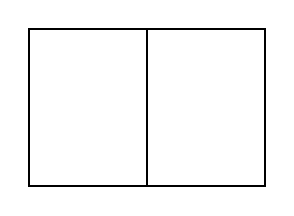
\begin{tikzpicture}
\draw [thick](0,0) rectangle (3,2);
\draw [thick](1.5,0) -- (1.5,2);
\end{tikzpicture}
\end{minipage}

\item A standard soda can is roughly cylindrical and holds $355$ cm$^3$ of liquid. What dimensions should the cylinder be to minimize the material needed to produce the can? Based on your dimensions, determine whether or not the standard can is produced to minimize the material costs.
\item Find the dimensions of a cylindrical can with a volume of $206$ in$^3$ that minimizes the surface area.

The ``\#10 can''is a standard sized can used by the restaurant industry that holds about $206$ in$^3$ with a diameter of $6 \frac{2}{16}$ in and height of $7$ in. Does it seem these dimensions where chosen with minimization in mind?

\item The strength $S$ of a wooden beam is directly proportional to its cross sectional  width $w$ and the square of its height $h$; that is, $S = kwh^2$ for some constant $k$. 

\noindent\begin{minipage}{\linewidth}
\centering
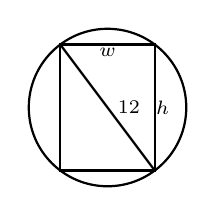
\begin{tikzpicture}
\draw [thick](0,0) circle (1cm);
\draw [thick](-.6,.8) -- node [pos=.5,right] {\scriptsize $12$} (.6,-.8);
\draw [thick](-.6,-.8) rectangle (.6,.8);
\draw (.7,0) node {\scriptsize $h$} (0,.7) node {\scriptsize $w$};
\end{tikzpicture}
\end{minipage}

Given a circular log with diameter of $12$ inches, what sized beam can be cut from the log with maximum strength?

\item A power line is to be run to an offshore facility in the manner described in Example~\ref{Ex:3.4.Eg3}. The offshore facility is $2$ miles at sea and $5$ miles along the shoreline from the power plant. It costs \$ $50,000$ per mile to lay a power line underground and \$ $80,000$ to run the line underwater. 

How much of the power line should be run underground to minimize the overall costs?
\item A power line is to be run to an offshore facility in the manner described in Example~\ref{Ex:3.4.Eg3}. The offshore facility is $5$ miles at sea and $2$ miles along the shoreline from the power plant. It costs $\$50,000$ per mile to lay a power line underground and $\$80,000$ to run the line underwater. 

How much of the power line should be run underground to minimize the overall costs?

\item A woman throws a stick into a lake for her dog to fetch; the stick is $20$ feet down the shore line and $15$ feet into the water from there. The dog may jump directly into the water and swim, or run along the shore line to get closer to the stick before swimming. The dog runs about $22$ ft/s and swims about $1.5$ ft/s. 

How far along the shore should the dog run to minimize the time it takes to get to the stick?

\item A woman throws a stick into a lake for her dog to fetch; the stick is $15$ feet down the shore line and $30$ feet into the water from there. The dog may jump directly into the water and swim, or run along the shore line to get closer to the stick before swimming. The dog runs about $22$ ft/s and swims about $1.5$ ft/s. 

How far along the shore should the dog run to minimize the time it takes to get to the stick? \textit{(Google ``calculus dog'' to learn more about a dog's ability to minimize times.)}

\item What are the dimensions of the rectangle with largest area that can be drawn inside the unit circle?

	\item A rectangular box with a square bottom and closed top is to be made from two materials.  The material for the side costs $\$1.50$ per square foot and the material for the bottom costs $\$3.00$ per square foot.  If you are willing to spend $\$15$ on the box, what is the largest volume it can contain?  Justify your answer completely using calculus.

\end{enumerate}

%------------------------------------------
% END OF EXERCISES ON FIRST PAGE
%------------------------------------------
\end{multicols*}
\end{adjustwidth*}

\clearpage

\begin{adjustwidth*}{}{-2.25in}
\setlength{\columnsep}{25pt}
\begin{multicols*}{2}\small

\begin{enumerate}[1),start=18]
	\item A farmer wants to start raising cows, horses, goats, and sheep, and desires to have a rectangular pasture for the animals to graze in.  However, no two different kinds of animals can graze together.  In order to minimize the amount of fencing she will need, she has decided to enclose a large rectangular area and then divide it into four equally sized pens, or grazing areas.  She has decided to purchase $7500$ ft of fencing.  What is the maximum possible area that each of the four pens will enclose?
	\item Two vertical towers of heights $60$ ft and $80$ ft stand on level ground, with their bases $100$ ft apart.  A cable that is stretched from the top of one pole to some point on the ground between the poles, and then to the top of the other pole.   What is the minimum possible length of cable required?  Justify your answer completely using calculus.
	\item A company is designing propane tanks that are cylindrical with hemispherical ends.   Assume that the company wants tanks that will hold $1000$ cubic feet of gas, and that the ends are more expensive to make, costing $\$5$ per square foot, while the cylindrical barrel between the ends costs $\$2$ per square foot.  Use calculus to determine the minimum cost to construct such a tank.
\end{enumerate}

%---------------------------------------------
% END OF EXERCISES ON SECOND PAGE
%---------------------------------------------
\end{multicols*}
\end{adjustwidth*}

\afterexercises 

\cleardoublepage
\section{The Mean Value Theorem}\label{S:3.5.MeanValue}

\begin{goals}
\item In a setting where the average rate of change of a function $f$ is known for a given interval, is there a value where the function has an instantaneous rate of change equal to the average rate of change? 
\end{goals} 

%--------------------------------------
% SUBSECTION INTRODUCTION
%--------------------------------------
\subsection*{Introduction}

We motivate this section with the following question: Suppose you leave your house and drive to your friend's house in a city $120$ miles away, completing the trip in two hours.  At any point during the trip do you necessarily have to be going $60$ miles per hour?

In answering this question, it is clear that the \textit{average} speed for the entire trip is $60$ mph (i.e. $120$ miles in $2$ hours), but the question is whether or not your \textit{instantaneous} speed is ever exactly $60$ mph. More simply, does your speedometer ever read exactly $60$ mph?  The answer, under some very reasonable assumptions, is ``yes.''

Let's now see why this situation is in a calculus text by translating it into mathematical symbols.

First assume that the function $y = f(t)$ gives the distance (in miles) traveled from your home at time $t$ (in hours) where $0\le t\le 2$.  In particular, this gives $f(0)=0$ and $f(2)=120$.  The slope of the secant line connecting the starting and ending points $(0,f(0))$ and $(2,f(2))$ is therefore 
$$
\frac{\Delta f}{\Delta t} = \frac{f(2)-f(0)}{2-0} = \frac{120-0}{2} = 60 \, \text{mph}.
$$

The slope at any point on the graph itself is given by the derivative $\fp(t)$.  So, since the answer to the question above is ``yes,'' this means that at some time during the trip, the derivative takes on the value of $60$ mph.  Symbolically, 
$$
\fp(c) = \frac{f(2)-f(0)}{2-0} = 60
$$
for some time $0\le c \le 2.$ 

\begin{pa} \label{PA:3.5}
On a recent vacation trip, Michelle traveled 200 miles on a toll road in 3 hours. 
\ba
	\item Plot points on the graph to represent Michelle's distance traveled, d, at a given time, t, where $t=0$ represents the time she started driving on the toll road.  
	\item Draw a possible distance function, d(t), on the graph.  
	\item On the second graph, plot Michelle's velocity, v(t). What was her average velocity during the trip?
	\item Based on the distance function, does she ever exceed this average velocity? If yes, explain by finding a time where she exceeds the average velocity. If not, explain why.
	\item If Michelle had to stop to pay her toll when entering the toll road, does she ever exceed the average velocity?
\ea
\end{pa} 
\afterpa

\begin{marginfigure}[-1.75cm]
\subfloat{\margingraphics{figures/3_5_PA1a.pdf}} 

\subfloat{\margingraphics{figures/3_5_PA1b.pdf}}
\caption{Axes for plotting $y = d(t)$ and $y=v(t)=d'(t)$.} \label{fig:3.5.PA1}
\end{marginfigure} %PREVIEW needs written toll road problem?

%-----------------------------------------------
% SUBSECTION MEAN VALUE THEOREM
%-----------------------------------------------
\subsection*{The Mean Value Theorem}

Can we generalize the velocity problem above to any function? In other words, given any function $y=f(x)$ and a range $a\leq x \leq b$, does the value of the derivative at some point between $a$ and $b$ have to match the slope of the secant line connecting the points $(a,f(a))$ and $(b,f(b))$?  Or equivalently, does the equation 
$\fp(c) = \frac{f(b)-f(a)}{b-a}$ have to hold for some $a < c < b$?

The following Activity will explore what properties $f$ must possess in order for the equation 
$\fp(c) = \frac{f(b)-f(a)}{b-a}$ to hold for some $a < c < b$.

\begin{marginfigure}[2cm] % MARGIN FIGURE
\begin{center}
\subfloat[$f_1(x) = 1/x^2$]{\includegraphics[scale=.3]{figs/3/activity351a.pdf}}
\hspace{.25cm}
\subfloat[$f_2(x) = |x|$]{\includegraphics[scale=.3]{figs/3/activity351b.pdf}}
\caption{The functions $f_1(x) = 1/x^2$ and $f_2(x) = |x|$ used in Activity~\ref{A:3.5.1}}
\label{fig:act351}
\end{center}
\end{marginfigure}

\begin{activity} \label{A:3.5.1}  Consider functions 
$$f_1(x)=\frac{1}{x^2}\quad \text{and} \quad f_2(x) = |x|$$ 
with $a=-1$ and $b=1$ as shown in Figure~\ref{fig:act351}-(a) and -(b), respectively. 
\ba
 \item For $f_1(x)$, find the slope of the secant line connecting the points $(a,f(a))$ and $(b,f(b))$.
 \item Find a value $c$ in $(a,b)$ such that $f_1'(c)$ equals the slope of the secant line connecting the points $(a,f(a))$ and $(b,f(b))$. Was it possible to find $c$? If not, what went wrong?
  \item For $f_2(x)$, find the slope of the secant line connecting the points $(a,f(a))$ and $(b,f(b))$.
 \item Find a value $c$ in $(a,b)$ such that $f_2'(c)$ equals the slope of the secant line connecting the points $(a,f(a))$ and $(b,f(b))$. Was it possible to find $c$? If not, what went wrong?
	\ea
\end{activity}

\aftera % ACTIVITY

So what went ``wrong''?  It may not be surprising to find that the discontinuity of $f_1$ and the corner of $f_2$ play a role.  If our functions had been continuous and differentiable, would we have been able to find that special value $c$? This is our motivation for the following theorem.

\concept{The Mean Value Theorem of Differentiation\label{C:MVT}}  % CONCEPT
{Let $y=f(x)$ be a continuous function on the closed interval $[a,b]$ and differentiable on the open interval $(a,b)$. There exists a value $c$, $a < c < b$, such that \index{Mean Value Theorem!of differentiation}\index{derivative!Mean Value Theorem}
$$
\fp(c) = \frac{f(b)-f(a)}{b-a}.
$$
That is, there is a value $c$ in $(a,b)$ where the instantaneous rate of change of $f$ at $c$ is equal to the average rate of change of $f$ on $[a,b]$.} % end concept

Note that the reasons that the functions in Activity\ref{A:3.5.1} fail are indeed that $f_1$ has a discontinuity on the interval $[-1,1]$ and $f_2$ is not differentiable at the origin.

We will give a proof of the Mean Value Theorem below. To do so, we use another theorem, called Rolle's Theorem, stated here.

\concept{Rolle's Theorem\label{C:Rolles}} % CONCEPT
{Let $f$ be continuous on $[a,b]$ and differentiable on $(a,b)$, where $f(a) = f(b)$. There is some $c$ in $(a,b)$ such that $\fp(c) = 0.$\index{Rolle's Theorem}} % end CONCEPT

\begin{marginfigure}[1cm] % MARGIN FIGURE
\margingraphics{figures/figmvt3}
\caption{A graph of $f(x) = x^3-5x^2+3x+5$, where $f(a) = f(b)$. Note the existence of $c$, where $a<c<b$, where $\fp(c)=0$.}\label{fig:mvt3}
\end{marginfigure}

Consider Figure \ref{fig:mvt3} where the graph of a function $f$ is given, where $f(a) = f(b)$. It should make intuitive sense that if $f$ is differentiable (and hence, continuous) that there would be a value $c$ in $(a,b)$ where $\fp(c)=0$; that is, there would be a local maximum or minimum of $f$ in $(a,b)$. Rolle's Theorem guarantees at least one; there may be more. 

Rolle's Theorem is really just a special case of the Mean Value Theorem. If $f(a) = f(b)$, then the \textit{average} rate of change on $(a,b)$ is $0$, and the theorem guarantees some $c$ where $\fp(c)=0$. We will prove Rolle's Theorem, then use it to prove the Mean Value Theorem.\\

\proof (Rolle's Theorem) Let $f$ be differentiable on $(a,b)$ where $f(a)=f(b)$. We consider two cases. 

\noindent\textbf{Case 1:} Consider the case when $f$ is constant on $[a,b]$; that is, $f(x) = f(a) = f(b)$ for all $x$ in $[a,b]$. Then $\fp(x) = 0$ for all $x$ in $[a,b]$, showing there is at least one value $c$ in $(a,b)$ where $\fp(c)=0$.

\noindent\textbf{Case 2:} Now assume that $f$ is not constant on $[a,b]$. The Extreme Value Theorem guarantees that $f$ has a maximal and minimal value on $[a,b]$, found either at the endpoints or at a critical value in $(a,b)$. Since $f(a)=f(b)$ and $f$ is not constant, it is clear that the maximum and minimum cannot \textit{both} be found at the endpoints. Assume, without loss of generality, that the maximum of $f$ is not found at the endpoints. Therefore there is a $c$ in $(a,b)$ such that $f(c)$ is the maximum value of $f$. Thus $c$ must be a critical number of $f$; since $f$ is differentiable, we have that $\fp(c) = 0$, completing the proof of the theorem. \hfill $\square$\\

\proof (Mean Value Theorem) Define the function $$g(x) = f(x) - \frac{f(b)-f(a)}{b-a}x.$$  We know $g$ is differentiable on $(a,b)$ and  continuous on $[a,b]$ since $f$ is. We can show $g(a)=g(b)$ (it is actually easier to show $g(b)-g(a)=0$, which suffices). We can then apply Rolle's theorem to guarantee the existence of $c \in (a,b)$ such that $g'(c) = 0$.  But note that $$0= g'(c) = \fp(c) - \frac{f(b)-f(a)}{b-a} \ ;$$ hence $$\fp(c) = \frac{f(b)-f(a)}{b-a},$$ which is what we sought to prove.\hfill $\square$\\

Going back to the very beginning of the section, we see that the only assumption we would need about our distance function $f(t)$ is that it be continuous and differentiable for $t$ from $0$ to $2$ hours (both reasonable assumptions).  By the Mean Value Theorem, we are guaranteed a time during the trip where our instantaneous speed is $60$ mph. This fact is used in practice. Some law enforcement agencies monitor traffic speeds while in aircraft. They do not measure speed with radar, but rather by timing individual cars as they pass over lines painted on the highway whose distances apart are known. The officer is able to measure the \textit{average} speed of a car between the painted lines; if that average speed is greater than the posted speed limit, the officer is assured that the driver exceeded the speed limit at some time.

Note that the Mean Value Theorem is an \textit{existence} theorem. It states that a special value $c$ \textit{exists}, but it does not give any indication about how to find it.  To do so, we must be able to solve equations, which sometimes can be very difficult.  The following example demonstrates the process for finding a special value $c$.



\begin{example} \label{Ex:3.5.Eg1}
Consider $f(x) = x^3+5x+5$ on $[-3,3]$. Find $c$ in $[-3,3]$ that satisfies the Mean Value Theorem.

\solution
The average rate of change of $f$ on $[-3,3]$ is:
		$$\frac{f(3)-f(-3)}{3-(-3)} = \frac{84}{6} = 14.$$
		
We want to find $c$ such that $\fp(c) = 14$. We find $\fp(x) = 3x^2+5$. We set this equal to $14$ and solve for $x$. 
		\begin{align*}
		3x^2 +5 &= 14\\
		x^2  &= 3\\
		x &= \pm \sqrt{3} \approx \pm 1.732
		\end{align*}
		
We have found $2$ values $c$ in $[-3,3]$ where the instantaneous rate of change is equal to the average rate of change; the Mean Value Theorem guaranteed at least one. In Figure~\ref{F:3.5.Ex1} $f$ is graphed with a dashed line representing the average rate of change; the lines tangent to $f$ at $x=\pm \sqrt{3}$ are also given. Note how these lines are parallel (i.e., have the same slope) as the dashed line.

\end{example}

\begin{marginfigure}[-8cm]
\margingraphics{figures/figmvt4} %APEX ex83
\caption{Demonstrating the Mean Value Theorem in Example~\ref{Ex:3.5.Eg1}}\label{F:3.5.Ex1}
\end{marginfigure} % EXAMPLE

In the next activty, we examine two other results based on the Mean Value Theorem.


\begin{activity} \label{A:3.5.2}  In this activity, we will discuss two important consequences of the Mean Value Theorem.  
\ba
 \item Suppose $f'(x)=0$ for $x$ in $[a,b]$. What can we say about $f(x)$ on the interval $[a,b]$?
 \item Given two functions $f$ and $g$ defined on $[a,b]$ such that $f'(x)=g'(x)$ for all $x$ in $[a,b]$, what can we say about the functions themselves? How are $f$ and $g$ related?
	\ea
\end{activity}

\aftera % ACTIVITY

The Mean Value Theorem has practical use (for instance, the speed monitoring application mentioned before) in the sciences and other applications.  However, it turns out that when we need the Mean Value Theorem in mathematics, existence is all we need, and it is mostly used to advance other theory.

%--------------
% SUMMARY
%--------------
\begin{summary}
\item If $f$ is a continuous function on the closed interval $[a,b]$ and differentiable on the open interval $(a,b)$. There exists a value $c$, $a < c < b$, such that $\fp(c) = \frac{f(b)-f(a)}{b-a}$, i.e. the instantaneous rate of change of $f$ at $c$ is equal to the average rate of change of $f$ on $[a,b]$.
\end{summary}

%--------------
% EXERCISES
%--------------
\begin{adjustwidth*}{}{-2.25in}
\textbf{{\large Exercises}}
\setlength{\columnsep}{25pt}
\begin{multicols*}{2}
\noindent Terms and Concepts \small
\begin{enumerate}[1)]
\item Explain in your own words what the Mean Value Theorem states.
\item Explain in your own words what Rolle's Theorem states.
\end{enumerate} 

\noindent {\normalsize Problems} \small

\noindent{\bf In exercises 3--10, a function $f(x)$ and interval $[a,b]$ are given.  Check if Rolle's Theorem can be applied, and if so, find $c$ in $[a,b]$ such that $f'(c) = 0$.}

\begin{enumerate}[1),resume]
\item $f(x) = 6$ on $[-1,1]$.
\item $f(x) = 6x$ on $[-1,1]$.
\item $f(x) = x^2+x-6$ on $[-3,2]$.
\item $f(x) = x^2+x-2$ on $[-3,2]$.
\item $f(x) = x^2+x$ on $[-2,2]$.
\item $f(x) = \sin x$ on $[\pi/6,5\pi/6]$.
\item $f(x) = \cos x$ on $[0,\pi]$.
\item $\ds f(x) = \frac{1}{x^2-2x+1}$ on $[0,2]$.
\end{enumerate}

\noindent{\bf In exercises 11-20, a function $f(x)$ and interval $[a,b]$ are given Check if the Mean Value Theorem can be applied, and if so, find a value $c$ guaranteed by the Mean Value Theorem.}

\begin{enumerate}[1),resume]
\item $\ds f(x) = x^2+3x-1$ on $[-2,2]$.
\item $\ds f(x) = 5x^2-6x+8$ on $[0,5]$.
\item $\ds f(x) = \sqrt{9-x^2}$ on $[0,3]$.
\item $\ds f(x) = \sqrt{25-x}$ on $[0,9]$.
\item $\ds f(x) = \ln x$ on $[1,5]$.
\item $\ds f(x) = \tan x$ on $[-\pi/4,\pi/4]$.
\item $\ds f(x) = x^3-2x^2+x+1$ on $[-2,2]$.
\item $\ds f(x) = 2x^3-5x^2+6x+1$ on $[-5,2]$.
\item $\ds f(x) = \sin^{-1} x$ on $[-1,1]$.
\item $\ds f(x) =\frac{x^2-9}{x^2-1}$ on $[0,2]$.
\end{enumerate}

\begin{enumerate}[1),resume]
\item Show that the equation $6x^4 -7x+1 =0$ does not have more
than two distinct real roots.
%\begin{answer}
%Seeking a contradiction, suppose that we have 3 real roots, call them
%$a$, $b$, and $c$. By Rolle's Theorem, $24x^3-7$ must have a root on
%both $(a,b)$ and $(b,c)$, but this is impossible as $24x^3-7$ has only
%one real root.
%\end{answer}

\item Let $f(x)$ be differentiable on $\mathbb{R}$. Suppose that $f'(x) \ne
0$ for every $x$. Prove that $f$ has at most one real root.
%\begin{answer}
%Seeking a contradiction, suppose that we have 2 real roots, call them
%$a$, $b$. By Rolle's Theorem, $f'(x)$ must have a root on $(a,b)$, but
%this is impossible.
%\end{answer}


\item Two runners start a race at the same time and finish in a tie. Prove that at some time during the race they have the same speed.
\end{enumerate}

%------------------------------------------
% END OF EXERCISES ON FIRST PAGE
%------------------------------------------
\end{multicols*}
\end{adjustwidth*}

\afterexercises 

\cleardoublepage
\section{The Tangent Line Approximation} \label{S:3.6.LinApprox}

\begin{goals}
\item What is the formula for the general tangent line approximation to a differentiable function $y = f(x)$ at the point $(a,f(a))$?
\item What is the principle of local linearity and what is the local linearization of a differentiable function $f$ at a point $(a,f(a))$?
\item How does knowing just the tangent line approximation tell us information about the behavior of the original function itself near the point of approximation?  How does knowing the second derivative's value at this point provide us additional knowledge of the original function's behavior?
\end{goals}

%--------------------------------------
% SUBSECTION INTRODUCTION
%--------------------------------------
\subsection*{Introduction}

Among all functions, linear functions are simplest.  One of the powerful consequences of a function $y = f(x)$ being differentiable at a point $(a,f(a))$ is that, up close, the function $y = f(x)$ is locally linear and looks like its tangent line at that point.  In certain circumstances, this allows us to approximate the original function $f$ with a simpler function $L$ that is linear: this can be advantageous when we have limited information about $f$ or when $f$ is computationally or algebraically complicated.  We will explore all of these situations in what follows.

It is essential to recall that when $f$ is differentiable at $x = a$, the value of $f'(a)$ provides the slope of the tangent line to $y = f(x)$ at the point $(a,f(a))$.  By knowing both a point on the line and the slope of the line we are thus able to find the equation of the tangent line.  Preview Activity~\ref{PA:3.6} will refresh these concepts through a key example and set the stage for further study.

\begin{marginfigure}[8cm]
\margingraphics{figures/1_8_PA1.eps}
\caption{Axes for plotting $y = g(x)$ and its tangent line to the point $(2,g(2))$.} \label{F:1.8.PA1}
\end{marginfigure}

\begin{pa} \label{PA:3.6}
Consider the function $y = g(x) = -x^2+3x+2$.

\ba
	\item Use the limit definition of the derivative to compute a formula for $y = g'(x)$.
	\item Determine the slope of the tangent line to $y = g(x)$ at the value $x = 2$.
	\item Compute $g(2)$.
	\item Find an equation for the tangent line to $y = g(x)$ at the point $(2,g(2))$.  Write your result in point-slope form. Recall that a line with slope $m$ that passes through $(x_0,y_0)$ has equation $y - y_0 = m(x - x_0)$, and this is the \emph{point-slope form} of the equation.
	\item On the axes provided in Figure~\ref{F:1.8.PA1}, sketch an accurate, labeled graph of $y = g(x)$ along with its tangent line at the point $(2,g(2))$.
\ea
\end{pa} 

\afterpa

 % PREVIEW

%--------------------------------------
% SUBSECTION TANGENT LINE	
%--------------------------------------
\subsection*{The tangent line}\index{tangent line!equation}

Given a function $f$ that is differentiable at $x = a$, we know that we can determine the slope of the tangent line to $y = f(x)$ at $(a,f(a))$ by computing $f'(a)$.  The resulting tangent line through $(a,f(a))$ with slope $m = f'(a)$ has its equation in point-slope form given by
$$y - f(a) = f'(a)(x-a),$$
which we can also express as $y = f'(a)(x-a) + f(a)$.  Note well: there is a major difference between $f(a)$ and $f(x)$ in this context.  The former is a constant that results from using the given fixed value of $a$, while the latter is the general expression for the rule that defines the function.  The same is true for $f'(a)$ and $f'(x)$: we must carefully distinguish between these expressions.  Each time we find the tangent line, we need to evaluate the function and its derivative at a fixed $a$-value.


\begin{marginfigure}[1cm] % MARGIN FIGURE
\margingraphics{figures/1_8_TanLine.eps}
\caption{A function $y = f(x)$ and its tangent line at the point $(a,f(a))$: at left, from a distance, and at right, up close.  At right, we label the tangent line function by $y = L(x)$ and observe that for $x $ near $a$, $f(x) \approx L(x)$.} \label{F:3.6.TanLine}
\end{marginfigure}

In Figure~\ref{F:3.6.TanLine}, we see a labeled plot of the graph of a function $f$ and its tangent line at the point $(a,f(a))$.  Notice how when we zoom in we see the local linearity of $f$ more clearly highlighted as the function and its tangent line are nearly indistinguishable up close.  This can also be seen dynamically in the java applet at \href{http://gvsu.edu/s/6J}{\texttt{http://gvsu.edu/s/6J}}.

%--------------------------------------
% SUBSECTION LOCAL LINEARIZATION	
%--------------------------------------
\subsection*{The local linearization} \index{local linearization}

A slight change in perspective and notation will enable us to be more precise in discussing how the tangent line to $y = f(x)$ at $(a,f(a))$ approximates $f$ near $x = a$.  Taking the equation for the tangent line and solving for $y$, we observe that the tangent line is given by
$$y = f'(a)(x-a) + f(a)$$
and moreover that this line is itself a function of $x$.  Replacing the variable $y$ with the expression $L(x)$, we call
$$L(x) = f'(a)(x-a) + f(a)$$
the \emph{local linearization of $f$} at the point $(a,f(a))$.  In this notation, it is particularly important to observe that $L(x)$ is nothing more than a new name for the tangent line, and that for $x$ close to $a$, we have that $f(x) \approx L(x)$.

Say, for example, that we know that a function $y = f(x)$ has its tangent line approximation given by $L(x) = 3 - 2(x-1)$ at the point $(1,3)$, but we do not know anything else about the function $f$.  If we are interested in estimating a value of $f(x)$ for $x$ near $1$, such as $f(1.2)$, we can use the fact that $f(1.2) \approx L(1.2)$ and hence
$$f(1.2) \approx L(1.2) = 3 - 2(1.2-1) = 3 - 2(0.2) = 2.6.$$
Again, much of the new perspective here is only in notation since $y = L(x)$ is simply a new name for the tangent line function.  In light of this new notation and our observations above, we note that since $L(x) = f(a) + f'(a)(x-a)$ and $L(x) \approx f(x)$ for $x$ near $a$, it also follows that we can write
$$f(x) \approx f(a) + f'(a)(x-a) \ \mbox{for} \  x \ \mbox{near} \ a.$$

The next activity explores some additional important properties of the local linearization $y = L(x)$ to a function $f$ at given $a$-value.

\begin{marginfigure}[6cm]
\margingraphics{figures/1_8_Act1.eps}
\caption{Axes for plotting $y = L(x)$ and $y = g(x)$.} \label{F:1.8.Act1}
\end{marginfigure}

\begin{activity} \label{A:3.6.1}
Suppose it is known that for a given differentiable function $y = g(x)$, its local linearization at the point where $a = -1$ is given by $L(x) = -2 + 3(x+1)$.
\ba
	\item Compute the values of $L(-1)$ and $L'(-1)$.
	\item What must be the values of $g(-1)$ and $g'(-1)$?  Why?
	\item Do you expect the value of $g(-1.03)$ to be greater than or less than the value of $g(-1)$?  Why?
	\item Use the local linearization to estimate the value of $g(-1.03)$.
	\item Suppose that you also know that $g''(-1) = 2.$  What does this tell you about the graph of $y = g(x)$ at $a = -1$?
	\item For $x$ near $-1$, sketch the graph of the local linearization $y = L(x)$ as well as a possible graph of $y = g(x)$ on the axes provided in Figure~\ref{F:1.8.Act1}.
\ea

\end{activity}

\begin{smallhint}
\ba
	\item Follow the rule for $L$.
	\item Recall that the form of the local linearization is $L(x) = g(a) + g'(a)(x-a)$.
	\item Is the function $g$ increasing or decreasing at $a = -1$?
	\item Remember that $g(-1.03) \approx L(-1.03)$.
	\item What does the second derivative tell you about the shape of a curve?
	\item Use your work above.
\ea
\end{smallhint}

\begin{bighint}
\ba
	\item Follow the rule for $L$ and note that you can easily compute $L'(x)$.
	\item Recall that the form of the local linearization is $L(x) = g(a) + g'(a)(x-a)$.  What is the value of $a$ for the given function $L$?
	\item Observe that the value of $g'(-1)$ tells you whether the function $g$ increasing or decreasing at $a = -1$.
	\item Remember that $g(-1.03) \approx L(-1.03)$ and you know a rule for $L(x)$.
	\item What does a positive second derivative tell you about the shape of a curve at a point?
	\item Use your work above, and think about the value, slope, and concavity of $y = g(x)$ at $a = -1$.
\ea
\end{bighint}




\aftera % ACTIVITY

As we saw in the example provided by Activity~\ref{A:3.6.1}, the local linearization $y = L(x)$ is a linear function that shares two important values with the function $y = f(x)$ that it is derived from.  In particular, observe that since $L(x) = f(a) + f'(a)(x-a)$, it follows that $L(a) = f(a)$.  In addition, since $L$ is a linear function, its derivative is its slope.  Hence, $L'(x) = f'(a)$ for every value of $x$, and specifically $L'(a) = f'(a)$.  Therefore, we see that $L$ is a linear function that has both the same value and the same slope as the function $f$ at the point $(a,f(a))$.

In situations where we know the linear approximation $y = L(x)$, we therefore know the original function's value and slope at the point of tangency.  What remains unknown, however, is the shape of the function $f$ at the point of tangency.  There are essentially four possibilities, as enumerated in Figure~\ref{F:3.6.Options}.  

\begin{marginfigure}[1cm] % MARGIN FIGURE
\margingraphics{figures/1_8_Options.eps}
\caption{Four possible graphs for a nonlinear differentiable function and how it can be situated relative to its tangent line at a point.} \label{F:3.6.Options}
\end{marginfigure}

These stem from the fact that there are three options for the value of the second derivative:  either $f''(a) <0$, $f''(a) = 0$, or $f''(a) > 0$.  If $f''(a) > 0$, then we know the graph of $f$ is concave up, and we see the first possibility on the left, where the tangent line lies entirely below the curve.  If $f''(a) < 0$, then we find ourselves in the second situation (from left) where $f$ is concave down and the tangent line lies above the curve.  In the situation where $f''(a) = 0$ and $f''$ changes sign at $x = a$, the concavity of the graph will change, and we will see either the third or fourth option\footnote{It is possible to have $f''(a) = 0$ and have $f''$ not change sign at $x = a$, in which case the graph will look like one of the first two options.}.  A fifth option (that is not very interesting) can occur, which is where the function $f$ is linear, and so $f(x) = L(x)$ for all values of $x$.

The plots in Figure~\ref{F:3.6.Options} highlight yet another important thing that we can learn from the concavity of the graph near the point of tangency: whether the tangent line lies above or below the curve itself.  This is key because it tells us whether or not the tangent line approximation's values will be too large or too small in comparison to the true value of $f$.  For instance, in the first situation in the leftmost plot in Figure~\ref{F:3.6.Options} where $f''(a) > 0$, since the tangent line falls below the curve, we know that $L(x) \le f(x)$ for all values of $x$ near $a$.

We explore these ideas further in the following activity.

\begin{marginfigure}[6cm]
\margingraphics{figures/1_8_Act2.eps}
\caption{At center, a graph of $y = f'(x)$; at left, axes for plotting $y = f(x)$; at right, axes for plotting $y = f''(x)$.} \label{F:1.8.Act2}
\end{marginfigure}

\begin{activity} \label{A:1.8.2}
This activity concerns a function $f(x)$ about which the following information is known:
\begin{itemize}
	\item $f$ is a differentiable function defined at every real number $x$
	\item $f(2) = -1$
	\item $y = f'(x)$ has its graph given in Figure~\ref{F:1.8.Act2}
\end{itemize}


Your task is to determine as much information as possible about $f$ (especially near the value $a = 2$) by responding to the questions below.
\ba
	\item Find a formula for the tangent line approximation, $L(x)$, to $f$ at the point $(2,-1)$.
	\item Use the tangent line approximation to estimate the value of $f(2.07)$.  Show your work carefully and clearly.
	\item Sketch a graph of $y = f''(x)$ on the righthand grid in Figure~\ref{F:1.8.Act2}; label it appropriately.
	\item Is the slope of the tangent line to $y = f(x)$ increasing, decreasing, or neither when $x = 2$?  Explain.
	\item Sketch a possible graph of $y = f(x)$ near $x = 2$ on the lefthand grid in Figure~\ref{F:1.8.Act2}.  Include a sketch of $y=L(x)$ (found in part (a)).  Explain how you know the graph of $y = f(x)$ looks like you have drawn it.   
	\item Does your estimate in (b) over- or under-estimate the true value of $f(2)$?  Why?
\ea
\end{activity}
\begin{smallhint}
\ba
	\item Find the value of $f'(2)$ from the given graph of $f$.
	\item Remember that $f(2.07) \approx L(2.07)$.
	\item The graph of $y = f''(x)$ is the derivative of the graph of $y = f'(x)$.
	\item Is $f'$ increasing, decreasing, or neither when $x = 2$? 
	\item Draw $y = L(x)$ first.  Then think about options for $f$ relative to the graph of $L$.  
	\item Does the tangent line lie above or below the graph of $y = f(x)$ at $(2,3)$?
\ea
\end{smallhint}
\begin{bighint}
\ba
	\item Find the value of $f'(2)$ from the given graph of $f$, and note that you are given that $f(2) = -1$.
	\item Remember that $f(2.07) \approx L(2.07)$.
	\item The graph of $y = f''(x)$ is the derivative of the graph of $y = f'(x)$.  Where must $f''(x) = 0$?  Where is $f''(x)$ positive?
	\item Is $f'$ increasing, decreasing, or neither when $x = 2$?  Use the given graph of $y = f'(x)$ to help you decide.
	\item Draw $y = L(x)$ first.  Then think about options for $f$ relative to the graph of $L$.  Is $f$ concave up or concave down before $x = 2$?  after $x = 2$?
	\item Does the tangent line lie above or below the graph of $y = f(x)$ at $(2,3)$?  You may have to consider values less than $x = 2$ and values greater than $x = 2$.
\ea
\end{bighint}
\begin{activitySolution}
\ba
	\item Since $f(2) = -1$ and $f'(2) = 2$, we have $L(x) = -1 + 2(x-2)$.
	\item Using our work in (a), $f(2.07) \approx L(2.07) = -1 + 2(2.07-2) = -1 + 2\cdot 0.07 = -0.86$.  
	\item See the plot below.
	\item Is the slope of the tangent line to $y = f(x)$ is increasing for $x < 2$ because $y = f'(x)$ is an increasing function on this interval.  Similarly, for $x > 2$, the slope of the tangent line to $y = f(x)$ is decreasing.  Right at $x = 2$, the slope of the tangent line to $y = f(x)$ is neither increasing nor decreasing.
	\item See the plot below.  Note that $y = f(x)$ is concave up for $x < 2$ since $f'$ is increasing on that interval, and $y = f(x)$ is concave down for $x > 2$ since $f'$ is decreasing there.  Hence $y = f(x)$ changes from concave up to concave down right at $x = 2$, which is also the point near 2 where the graph of $y = f(x)$ is steepest.
	\item Because the tangent line to $y = f(x)$ lies above the graph  of $f$ to the right of $x = 2$, our estimate of $f(2.07)$ is too large -- the local linearization overshoots the true value of $f$ at this point.
\ea

\begin{center}
\includegraphics{figures/1_8_Act2.eps}
\end{center}
\end{activitySolution}
\aftera % ACTIVITY

The idea that a differentiable function looks linear and can be well-approximated by a linear function is an important one that finds wide application in calculus.  For example, by approximating a function with its local linearization, it is possible to develop an effective algorithm to estimate the zeroes of a function.  Local linearity also helps us to make further sense of certain challenging limits.  For instance, we have seen that a limit such as
$$\lim_{x \to 0} \frac{\sin(x)}{x}$$
is indeterminate because both its numerator and denominator tend to $0$.  While there is no algebra that we can do to simplify $\frac{\sin(x)}{x}$, it is straightforward to show that the linearization of $f(x) = \sin(x)$ at the point $(0,0)$ is given by $L(x) = x$.  Hence, for values of $x$ near $0$, $\sin(x) \approx x$.  As such, for values of $x$ near $0$, 
$$\frac{\sin(x)}{x} \approx \frac{x}{x} = 1,$$
which makes plausible the fact that $$\lim_{x \to 0} \frac{\sin(x)}{x} = 1.$$
These ideas and other applications of local linearity will be explored later on in our work.

%--------------------------------------
% SUBSECTION DIFFERENTIALS
%--------------------------------------
\subsection*{Differentials}

Recall that the derivative of a function $f$ can be used to find the slopes of lines tangent to the graph of $f$. At $x=a$, the tangent line to the graph of $f$ has equation $$y = f(a) + \fp(a)(x-a).$$
The tangent line can be used to find good approximations of $f(x)$ for values of $x$ near $a$. 

%For instance, we can approximate $\sin 1.1$ using the tangent line to the graph of $f(x)=\sin x$ at $x=\pi/3 \approx 1.05.$ Recall that $\sin (\pi/3) = \sqrt{3}/2 \approx 0.866$, and $\cos (\pi/3) = 1/2$. Thus the tangent line to $f(x) = \sin x$ at $x=\pi/3$ is: $$ \ell(x) = \frac12(x-\pi/3)+0.866.$$
%
%\begin{marginfigure}[-6cm] % MARGIN FIGURE
%\subfloat[]{\margingraphics{figures/figdiffal1a}}
%
%\subfloat[]{\margingraphics{figures/figdiffal1}}
%\caption{Graphing $f(x) = \sin x$ and its tangent line at $x=\pi/3$ in order to estimate $\sin 1.1$.}\label{fig:diffal1}
%\end{marginfigure}
%
%In Figure \ref{fig:diffal1}(a), we see a graph of $f(x) = \sin x$ graphed along with its tangent line at $x=\pi/3$. The small rectangle shows the region that is displayed in Figure \ref{fig:diffal1}(b). In this figure, we see how we are approximating $\sin 1.1$ with the tangent line, evaluated at $1.1$. Together, the two figures show how close these values are.
%
%Using this line to approximate $\sin 1.1$, we have:
%\begin{align*}
%\ell(1.1) &= \frac12(1.1-\pi/3)+0.866 \\
%&= \frac12(0.053)+0.866 = 0.8925.
%\end{align*}
%(We leave it to the reader to see how good of an approximation this is.)

We now generalize this concept. Given $f(x)$ and an $x$--value $a$,  the tangent line is $L(x) = f(a) + \fp(a)(x-a)$. Clearly, $L(a) = f(a)$. Let $\dx$ be a small number, representing a small change in $x$ value. We assert that:
$$f(a+\dx) \approx L(a+\dx),$$ since the tangent line to a function approximates well the values of that function near $x=a$. 

As the $x$ value changes from $a$ to $a+\dx$, the $y$ value of $f$ changes from $f(a)$ to $f(a+\dx)$. We call this change of $y$ value $\dy$. That is:
$$\dy = f(a+\dx)-f(a).$$
Replacing $f(a+\dx)$ with its tangent line approximation, we have 
\begin{align} \dy &\approx L(a+\dx) - f(a) \notag\\
&= \fp(a)\big((a+\dx)-a\big)+f(a) - f(a)\notag \\
&=\fp(a)\dx		\label{eq:differential}
\end{align}

This final equation is important; we'll come back to it in a moment.

We introduce two new variables, $dx$ and $dy$ in the context of a formal definition. %We defined $dx = \dx$; that is, it is a small change in $x$. We define

\definition{Differentials of $x$ and $y$} % DEFINITION
{Let $y=f(x)$ be differentiable. The \textbf{differential of $x$}, denoted $dx$, is any nonzero real number (usually taken to be a small number).\index{differential}\index{derivative!differential} The \textbf{differential of $y$}, denoted $dy$, is $$dy = \fp(x)dx.$$
} % end definition

It is helpful to organize our new concepts and notations in one place.

\concept{Differential Notation\index{differential!notation}} % CONCEPT
{Let $y = f(x)$ be a differentiable function. 
\ba
\item $\dx$ represents a small, nonzero change in $x$ value.
\item $dx$ represents a small, nonzero change in $x$ value (i.e., $\dx = dx$).
\item $\dy$ is the change in $y$ value as $x$ changes by $\dx$; hence $$\dy = f(x+\dx)-f(x).$$
\item $dy = \fp(x)dx$ which, by Equation (\ref{eq:differential}), is an \textit{approximation} of the change in $y$ value as $x$ changes by $\dx$; $dy \approx \dy$; see Figure~\ref{fig:differentials}.
\ea
} % end concept

\begin{marginfigure}[-3cm] % MARGIN FIGURE
\margingraphics{figs/3/differentials.pdf}
\caption{A graph describing the relationship of differentials.}
\label{fig:differentials}
\end{marginfigure}

What is the value of differentials? Like many mathematical concepts, differentials provide both practical and theoretical benefits. We explore both here.

\begin{example} \label{Ex:3.6.Eg1}
Consider $f(x) = x^2$. Knowing $f(3) = 9$, approximate $f(3.1)$.

\solution The $x$ value is changing from $x=3$ to $x=3.1$; therefore, we see that $dx=0.1$. If we know how much the $y$ value changes from $f(3)$ to $f(3.1)$ (i.e., if we know $\dy$), we will know exactly what $f(3.1)$ is (since we already know $f(3)$). We can approximate $\dy$ with $dy$.
\begin{align*} 
\dy &\approx dy \\
&= \fp(3)dx \\
&= 2\cdot 3\cdot 0.1 = 0.6.
\end{align*}

We expect the $y$ value to change by about $0.6$, so we approximate $f(3.1) \approx 9.6.$

We leave it to the reader to verify this, but the preceding discussion links the differential to the tangent line of $f(x)$ at $x=3$. One can verify that the tangent line, evaluated at $x=3.1$, also gives $y=9.6$.
\end{example} % EXAMPLE

Of course, it is easy to compute the actual answer (by hand or with a calculator): $3.1^2 = 9.61.$ (Before we get too cynical and say ``Then why bother?'', note our approximation is \textit{really} good!)

So why bother?

In ``most'' real life situations, we do not know the function that describes a particular behavior. Instead, we can only take measurements of how things change -- measurements of the derivative.

Imagine water flowing down a winding channel. It is easy to measure the speed and direction (i.e., the \textit{velocity}) of water at any location. It is very hard to create a function that describes the overall flow, hence it is hard to predict where a floating object placed at the beginning of the channel will end up. However, we can \textit{approximate} the path of an object using differentials. Over small intervals, the path taken by a floating object is essentially linear. Differentials allow us to approximate the true path by piecing together lots of short, linear paths. This technique is called Euler's Method, studied in introductory Differential Equations courses.

We use differentials once more to approximate the value of a function. Even though calculators are very accessible, it is neat to see how these techniques can sometimes be used to easily compute something that looks rather hard.

\begin{example} \label{Ex:3.6.Eg2}
Approximate $\sqrt{4.5}$.

\solution We expect $\sqrt{4.5} \approx 2$, yet we can do better. Let $f(x) = \sqrt{x}$, and let $c=4$. Thus $f(4) = 2$. We can compute $\fp(x) = 1/(2\sqrt{x})$, so $\fp(4) = 1/4$. 

We approximate the difference between $f(4.5)$ and $f(4)$ using differentials, with $dx = 0.5$:
$$f(4.5)-f(4) = \dy \approx dy = \fp(4)\cdot dx = 1/4 \cdot 1/2 = 1/8 = 0.125.$$
The approximate change in $f$ from $x=4$ to $x=4.5$ is $0.125$, so we approximate $\sqrt{4.5} \approx 2.125.$
\end{example} % EXAMPLE

Differentials are important when we discuss \textit{integration}. When we study that topic, we will use notation such as $$\int f(x)\ dx$$ quite often. While we don't discuss here what all of that notation means, note the existence of the differential $dx$. Proper handling of \textit{integrals} comes with proper handling of differentials. 

In light of that, we practice finding differentials in general.

\begin{example} \label{Ex:3.6.Eg3}
In each of the following, find the differential $dy$.
\begin{center}
1) $y = \sin x$ \qquad\quad 2) $y = e^x(x^2+2)$ \quad\qquad 3) $y = \sqrt{x^2+3x-1}$
\end{center}

\solution
\begin{enumerate}[1)]
\item $y = \sin x$:	\quad As $f(x) = \sin x$, $\fp(x) = \cos x$. Thus $$dy = \cos (x)dx.$$

\item $y = e^x(x^2+2)$:\quad Let $f(x) = e^x(x^2+2)$. We need $\fp(x)$, requiring the Product Rule. 

We have $\fp(x) = e^x(x^2+2) + 2xe^x$, so $$dy = (e^x(x^2+2) + 2xe^x)dx.$$

\item $y = \sqrt{x^2+3x-1}$:\quad	Let $f(x) = \sqrt{x^2+3x-1}$; we need $\fp(x)$, requiring the Chain Rule.

We have $\ds \fp(x) = \frac{1}{2}(x^2+3x-1)^{-\frac12}(2x+3) = \frac{2x+3}{2\sqrt{x^2+3x-1}}.$ Thus 
$$ dy = \frac{(2x+3)dx}{2\sqrt{x^2+3x-1}}.$$
\end{enumerate}
\end{example} % EXAMPLE

Finding the differential $dy$ of $y=f(x)$ is really no harder than finding the derivative of $f$; we just \textit{multiply} $\fp(x)$ by $dx$. It is important to remember that we are not simply adding the symbol ``$dx$'' at the end.

We have seen a practical use of differentials as they offer a good method of making certain approximations. Another use is \textit{error propagation.} Suppose a length is measured to be $x$, although the actual value is $x+\dx$ (where we hope $\dx$ is small). This measurement of $x$ may be used to compute some other value; we can think of this as $f(x)$ for some function $f$. As the true length is $x+\dx$, one really should have computed $f(x+\dx)$. The difference between $f(x)$ and $f(x+\dx)$ is the propagated error. 

How close are $f(x)$ and $f(x+\dx)$? This is a difference in ``y'' values; $$f(x+\dx)-f(x) = \dy \approx dy.$$ We can approximate the propagated error using differentials.

\begin{example} \label{Ex:3.6.Eg4}
A steel ball bearing is to be manufactured with a diameter of 2cm. The manufacturing process has a tolerance of $\pm 0.1$ mm in the diameter. Given that the density of steel is about $7.85$ g/cm$^3$, estimate the propagated error in the mass of the ball bearing.

\solution The mass of a ball bearing is found using the equation mass = volume $\times$ density. In this situation the mass function is a product of the radius of the ball bearing, hence it is $m = 7.85\frac43\pi r^3$. The differential of the mass is $$dm = 31.4\pi r^2 dr.$$ The radius is to be $1$ cm; the manufacturing tolerance in the radius is $\pm 0.05$ mm, or $\pm 0.005$ cm. The propagated error is approximately:
\begin{align*}
\Delta m & \approx dm \\
&= 31.4\pi (1)^2 (\pm 0.005) \\
&= \pm 0.493\text{ g}
\end{align*}
Is this error significant? It certainly depends on the application, but we can get an idea by computing the \textit{relative error}. The ratio between amount of error to the total mass is
\begin{align*}
\frac{dm}{m} &= \pm \frac{0.493}{7.85\frac43\pi} \\
&=\pm \frac{0.493}{32.88}\\
&=\pm 0.015,
\end{align*}
or $\pm 1.5$\%. 

We leave it to the reader to confirm this, but if the diameter of the ball was supposed to be $10$ cm, the same manufacturing tolerance would give a propagated error in mass of $\pm12.33$ g, which corresponds to a \textit{percent error} of $\pm0.188$\%. While the amount of error is much greater ($12.33 > 0.493$), the percent error is much lower.
\end{example} % EXAMPLE

\clearpage

%-------------
% SUMMARY
%-------------
\begin{summary}
\item The tangent line to a differentiable function $y = f(x)$ at the point $(a,f(a))$ is given in point-slope form by the equation
$$y - f(a) = f'(a)(x-a).$$
\item The principle of local linearity tells us that if we zoom in on a point where a function $y = f(x)$ is differentiable, the function should become indistinguishable from its tangent line.  That is, a differentiable function looks linear when viewed up close.  We rename the tangent line to be the function $y = L(x)$ where $L(x) = f(a) + f'(a)(x-a)$ and note that $f(x) \approx L(x)$ for all $x$ near $x = a$.
\item If we know the tangent line approximation $L(x) = f(a) + f'(a)(x-a)$, then because $L(a) = f(a)$ and $L'(a) = f'(a)$, we also know both the value and the derivative of the function $y = f(x)$ at the point where $x = a$.  In other words, the linear approximation tells us the height and slope of the original function.  If, in addition, we know the value of $f''(a)$, we then know whether the tangent line lies above or below the graph of $y = f(x)$ depending on the concavity of $f$.
\end{summary}

\clearpage

%--------------
% EXERCISES
%--------------
\begin{adjustwidth*}{}{-2.25in}
\textbf{{\large Exercises}}
\setlength{\columnsep}{25pt}
\begin{multicols*}{2}
\noindent Terms and Concepts \small
\begin{enumerate}[1)]
\item T/F: Given a differentiable function $y=f(x)$, we are generally free to choose a value for $dx$, which then determines the value of $dy$.
\item T/F: The symbols ``$dx$'' and ``$\dx$'' represent the same concept.
\item T/F: The symbols ``$dy$'' and ``$\dy$'' represent the same concept.
\item T/F: Differentials are important in the study of integration.
\item When could the linearization of a function $f(x)$ at $x=a$ be a constant function?
\item How are differentials and tangent lines related?
\end{enumerate} 

\noindent {\normalsize Problems} \small

\noindent{\bf In exercises 7--11, use differentials to approximate the given value by hand.}

\begin{enumerate}[1),resume]
\item $2.05^2$
\item $5.1^3$
\item $\sqrt{16.5}$
\item $\sqrt[3]{63}$
\item $\sin 3$

\item A certain function $y=p(x)$ has its local linearization at $a = 3$ given by $L(x) = -2x + 5$.

\ba
	\item What are the values of $p(3)$ and $p'(3)$?  Why?
	\item Estimate the value of $p(2.79)$.
	\item Suppose that $p''(3) = 0$ and you know that $p''(x) < 0$ for $x < 3$.  Is your estimate in (b) too large or too small?
	\item Suppose that $p''(x) > 0$ for $x > 3$.  Use this fact and the additional information above to sketch an accurate graph of $y = p(x)$ near $x = 3$.  Include a sketch of $y = L(x)$ in your work.
\ea

%ITEM
\item A potato is placed in an oven, and the potato's temperature $F$ (in degrees Fahrenheit) at various points in time is taken and recorded in the following table. Time $t$ is measured in minutes.

\scalebox{.9}{
\begin{tabular}{|c||c|c|c|c|c|c|c|}
\hline
$t$ & $0$ & $15$ & $30$ & $45$ & $60$ & $75$ & $90$ \\ \hline% $F(t)$ \\ \hline \hline
$F(t)$ & $70$ & $180.5$ & $251$ & $296$ & $324.5$ & $342.8$ & $354.5$ \\ \hline
\end{tabular}
} % end scalebox

%\begin{tabular}{| l || l |}
%\hline
%$t$ & $F(t)$ \\ \hline \hline
%0 & 70\\ \hline
%15 & 180.5 \\ \hline
%30 & 251 \\ \hline
%45 & 296 \\ \hline
%60 & 324.5 \\ \hline
%75 & 342.8 \\ \hline
%90 & 354.5  \\ \hline
%\end{tabular}

\ba
	\item Use a central difference to estimate $F'(60)$.  Use this estimate as needed in subsequent questions.
	\item Find the local linearization $y = L(t)$ to the function $y = F(t)$ at the point where $a = 60$.
	\item Determine an estimate for $F(63)$ by employing the local linearization.  
	\item Do you think your estimate in (c) is too large or too small?  Why?
\ea

%ITEM
\item An object moving along a straight line path has a differentiable position function $y = s(t)$.  It is known that at time $t = 9$ seconds, the object's position is $s = 4$ feet (measured from its starting point at $t = 0$).  Furthermore, the object's instantaneous velocity at $t = 9$ is $-1.2$ feet per second, and its acceleration at the same instant is $0.08$ feet per second per second.

\ba
	\item Use local linearity to estimate the position of the object at $t = 9.34$.
	\item Is your estimate likely too large or too small?  Why?
	\item In everyday language, describe the behavior of the moving object at $t = 9$.  Is it moving toward its starting point or away from it? Is its velocity increasing or decreasing?
\ea

%ITEM
\item For a certain function $f$, its derivative is known to be $f'(x) = (x-1)e^{-x^2}$.  Note that you do not know a formula for $y = f(x)$.
\ba  
  	\item At what $x$-value(s) is $f'(x) = 0$?  Justify your answer algebraically, but include a graph of $f'$ to support your conclusion.
	\item Reasoning graphically, for what intervals of $x$-values is $f''(x) > 0$?  What does this tell you about the  behavior of the original function $f$?  Explain.
	\item Assuming that $f(2) = -3$, estimate the value of $f(1.88)$ by finding and using the tangent line approximation to $f$ at $x=2$.  Is your estimate larger or smaller than the true value of $f(1.88)$?  Justify your answer.
\ea
\end{enumerate}

\noindent{\bf In exercises 16--25, compute the differential.}

\begin{enumerate}[1),resume]
\item $y=x^2+3x-5$
\item $y=x^7-x^5$
\item $\ds y=\frac{1}{4x^2}$
\item $\ds y=(2x+\sin x)^2$
\item $\ds y=x^2e^{3x}$
\item $\ds y=\frac{4}{x^4}$
\item $\ds y=\frac{2x}{\tan x + 1}$
\item $\ds y=\ln (5x)$
\item $\ds y=e^x\sin x$
\item $\ds y=\cos (\sin x)$
\end{enumerate}

%------------------------------------------
% END OF EXERCISES ON FIRST PAGE
%------------------------------------------
\end{multicols*}
\end{adjustwidth*}

\clearpage

\begin{adjustwidth*}{}{-2.25in}
\setlength{\columnsep}{25pt}
\begin{multicols*}{2}\small

\begin{enumerate}[1),start=26]
\item A set of plastic spheres are to be made with a diameter of 1cm. If the manufacturing process is accurate to 1mm, what is the propagated error in volume of the spheres?

\item The distance, in feet, a stone drops in $t$ seconds is given by $d(t) = 16t^2$. The depth of a hole is to be approximated by dropping a rock and listening for it to hit the bottom. What is the propagated error if the time measurement is accurate to $2/10^{\text{ths}}$ of a second and the measured time is:
	\ba
	\item 2 seconds?
	\item	5 seconds?
	\ea

\item What is the propagated error in the measurement of the cross sectional area of a circular log if the diameter is measured at $15''$, accurate to $1/4''$?

\item A wall is to be painted that is $8'$ high and is measured to be $10',\ 7''$ long. Find the propagated error in the measurement of the wall's surface area if the measurement is accurate to $1/2''$. 

\item \label{exer:04_04_ex_34}The length $l$ of a long wall is to be calculated by measuring the angle $\theta$ shown in the diagram (not to scale). Assume the formed triangle is an isosceles triangle. The measured angle is $143^\circ$, accurate to $1^\circ$. 

\begin{minipage}{\linewidth}
\centering
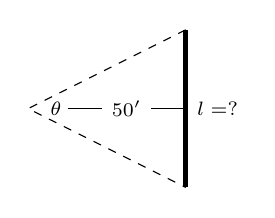
\begin{tikzpicture}
\draw [ultra thick] (1,-1) -- node [pos=.5,right] {\scriptsize $l=$?}(1,1);
\draw [dashed] (1,1) -- (-1,0) node [xshift=10pt] {\scriptsize $\theta$} -- (1,-1);
\draw (-.5,0) -- node [pos=.5,draw=white,fill=white] {\scriptsize $50'$} (1,0);
\end{tikzpicture}
\end{minipage}

\begin{enumerate}
\item		What is the measured length of the wall?
\item		What is the propagated error? 
\item		What is the percent error?
%\item		What is a key assumption about the location where the angle is measured? 
\end{enumerate}

\item \label{exer:04_04_ex_35} The length $l$ of a long wall is to be approximated. The angle $\theta$, as shown in the diagram (not to scale), is measured to be $85.2^\circ$, accurate to $1^\circ$. Assume that the triangle formed is a right triangle.

\begin{minipage}{\linewidth}
\centering
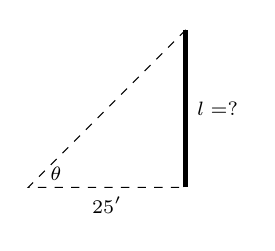
\begin{tikzpicture}
\draw [ultra thick] (1,-1) -- node [pos=.5,right] {\scriptsize $l=$?}(1,1);
\draw [dashed] (1,1) -- (-1,-1) node [xshift=10pt,yshift=5pt] {\scriptsize $\theta$} -- node [pos=.5,below] {\scriptsize $25'$} (1,-1);
%\draw (-.5,0) -- node [pos=.5,draw=white,fill=white] {\scriptsize $50'$} (1,0);
\end{tikzpicture}
\end{minipage}

\begin{enumerate}
\item		What is the measured length $l$ of the wall?
\item		What is the propagated error? 
\item		What is the percent error?
\end{enumerate}

\item \label{exer:04_04_ex_36} Answer the questions of Exercise \ref{exer:04_04_ex_35}, but with a measured angle of $71.5^\circ$, accurate to $1^\circ$, measured from a point $100'$ from the wall.

\item The length of the walls in Exercises \ref{exer:04_04_ex_35} -- \ref{exer:04_04_ex_34} are essentially the same. Which setup gives the most accurate result?

\item Consider the setup in Exercises \ref{exer:04_04_ex_34}. This time, assume the angle measurement of $143^\circ$ is exact but the measured $50'$ from the wall is accurate to $6''$. What is the approximate percent error?

%\item Use differentials to estimate the amount of paint needed to
%apply a coat of paint 0.02 cm thick to a sphere with diameter $40$
%meters. (Recall that the volume of a sphere of radius $r$ is $V
%=(4/3)\pi r^3$. Notice that you are given that $dr=0.02$.)
%%% \begin{answer} $dV=8\pi/25$

\end{enumerate}

\noindent{\bf Marginal Analysis.}

Differentials are used in economics to approximate changes in revenue, cost and profit. The  total revenue, $R$, for selling $x$ units of a product is given by
\[ R=xp\]  
When the number of units increases by one, the change in $x$ is $\delta x=1$, and the change in $R$ is \[ dR = \frac{dR}{dx} dx. \]
The differential $dR$ is the change in revenue that accompanies the sale of one additional unit and is called \emph{marginal revenue}. Similarly, differentials can be used to find the marginal profit, $dP$, and the marginal cost, $dC$. 
\begin{enumerate}[1),start=35]
\item		The demand function for a product is modeled by $p=\sqrt{400-x}$. What is the marginal revenue as sales increase from $256$ units to $257$ units?
\item		The profit derived from selling $x$ units of an item is modeled by $P=-0.5x^3+2500x-6000$. What is the marginal profit as sales increase from $50$ units to $51$ units?
\item		The cost of producing $x$ units of an item is modeled by $C=0.05x^2+4x+10$. What is the marginal cost as production increases from $12$ units to $13$ units?
\item 		Suppose the demand for a product is equal to the inverse of the square of the price. Find the marginal revenue when the price is $\$10$ per unit.
\end{enumerate}

%------------------------------------------------
% END OF EXERCISES ON SECOND PAGE
%------------------------------------------------
\end{multicols*}
\end{adjustwidth*}

\afterexercises 

\cleardoublepage
\section{Using Derivatives to Evaluate Limits} \label{S:3.7.LHR}

\begin{goals}
\item How can derivatives be used to help us evaluate indeterminate limits of the form $\frac{0}{0}$?
\item What does it mean to say that $\lim_{x \to \infty} f(x) = L$ and $\lim_{x \to a} f(x) = \infty$?
\item How can derivatives assist us in evaluating indeterminate limits of the form $\frac{\infty}{\infty}$?
\end{goals}

%--------------------------------------
% SUBSECTION INTRODUCTION
%--------------------------------------
\subsection*{Introduction}

Because differential calculus is based on the definition of the derivative, and the definition of the derivative involves a limit, there is a sense in which all of calculus rests on limits.  In addition, the limit involved in the limit definition of the derivative is one that always generates an indeterminate form of $\frac{0}{0}$.  If $f$ is a differentiable function for which $f'(x)$ exists, then when we consider
$$f'(x) = \lim_{h \to 0} \frac{f(x+h)-f(x)}{h},$$
it follows that not only does $h \to 0$ in the denominator, but also $(f(x+h)-f(x)) \to 0$ in the numerator, since $f$ is continuous.   Thus, the fundamental form of the limit involved in the definition of $f'(x)$ is $\frac{0}{0}$.  Remember, saying a limit has an indeterminate form only means that we don't yet know its value and have more work to do:  indeed, limits of the form $\frac{0}{0}$ can take on any value, as is evidenced by evaluating $f'(x)$ for varying values of $x$ for a function such as $f'(x) = x^2$.

Of course, we have learned many different techniques for evaluating the limits that result from the derivative definition, and including a large number of shortcut rules that enable us to evaluate these limits quickly and easily.  In this section, we turn the situation upside-down:  rather than using limits to evaluate derivatives, we explore how to use derivatives to evaluate certain limits.  This topic will combine several different ideas, including limits, derivative shortcuts, local linearity, and the tangent line approximation.

\begin{pa} \label{PA:3.7}
Let $h$ be the function given by $\ds h(x) = \frac{x^5 + x - 2}{x^2 - 1}$.
\ba
	\item What is the domain of $h$?
	\item Explain why $\displaystyle\lim_{x \to 1} \frac{x^5 + x
- 2}{x^2 - 1}$ results in an indeterminate form.
	\item Next we will investigate the behavior of both the numerator and denominator of $h$ near the point where $x = 1$.  Let $f(x) = x^5 + x - 2$
and $g(x) = x^2 - 1$. Find the local linearizations of $f$ and $g$ at $a = 1$, and call these functions $L_f(x)$ and $L_g(x)$, respectively.
	\item Explain why $\ds h(x) \approx \frac{L_f(x)}{L_g(x)}$ for $x$ near $a = 1$.
	\item Using your work from (c) and (d), evaluate 
	$$\lim_{x \to 1} \frac{L_f(x)}{L_g(x)}.$$
	What do you think your result tells us about $\ds \lim_{x \to 1} h(x)$?
	\item Investigate the function $h(x)$ graphically and numerically near $x = 1$.  What do you think is the value of $\ds \lim_{x \to 1} h(x)$?
\ea
\end{pa} 
\afterpa % PREVIEW ACTIVITY

%-------------------------------------------------------------------------------------------------------------------
% SUBSECTION USING DERIVATIVES TO EVALUATE INDETERMINATE LIMITS OF THE FORM 0/0
%-------------------------------------------------------------------------------------------------------------------
\subsection*{Using derivatives to evaluate indeterminate limits of the form $\frac{0}{0}$.}

The fundamental idea of Preview Activity~\ref{PA:3.7} -- that we can evaluate an indeterminate limit of the form $\frac{0}{0}$ by replacing each of the numerator and denominator with their local linearizations at the point of interest -- can be generalized in a way that enables us to easily evaluate a wide range of limits.  We begin by assuming that we have a function $h(x)$ that can be written in the form $h(x) = \frac{f(x)}{g(x)}$ where $f$ and $g$ are both differentiable at $x=a$ and for which $f(a) = g(a) = 0$.  We are interested in finding a way to evaluate the indeterminate limit given by
$\ds \lim_{x \to a} h(x).$

\begin{marginfigure} % MARGIN FIGURE
\margingraphics{figures/2_8_LHR.eps}
\caption{At left, the graphs of $f$ and $g$ near the value $a$, along with their tangent line approximations $L_f$ and $L_g$ at $x = a$.  At right, zooming in on the point $a$ and the four graphs.} \label{F:2.8.LHR}
\end{marginfigure}

In Figure~\ref{F:2.8.LHR}, we see a visual representation of the situation involving such functions $f$ and $g$.  In particular, we see that both $f$ and $g$ have an $x$-intercept at the point where $x = a$.  In addition, since each function is differentiable, each is locally linear, and we can find their respective tangent line approximations $L_f$ and $L_g$ at $x = a$, which are also shown in the figure.  Since we are interested in the limit of $\frac{f(x)}{g(x)}$ as $x \to a$, the individual behaviors of $f(x)$ and $g(x)$ as $x \to a$ are key to understand.  Here, we take advantage of the fact that each function and its tangent line approximation become indistinguishable as $x \to a$.

First, let's reall that $L_f(x) = f'(a)(x-a) + f(a)$ and $L_g(x) = g'(a)(x-a) +g(a)$.  The critical observation we make is that when taking the limit, because $x$ is getting arbitrarily close to $a$, we can replace $f$ with $L_f$ and replace $g$ with $L_g$, and thus we observe that
\begin{eqnarray*}
\lim_{x \to a} \frac{f(x)}{g(x)} & = & \lim_{x \to a} \frac{L_f(x)}{L_g(x)} \\
& = & \lim_{x \to a} \frac{f'(a)(x-a) + f(a)}{g'(a)(x-a) + g(a)}.
\end{eqnarray*}
Next, we remember a key fundamental assumption: that both $f(a) = 0$ and $g(a) = 0$, as this is precisely what makes the original limit indeterminate.  Substituting these values for $f(a)$ and $g(a)$ in the limit above, we now have
\begin{eqnarray*}
\lim_{x \to a} \frac{f(x)}{g(x)} & = & \lim_{x \to a} \frac{f'(a)(x-a)}{g'(a)(x-a)} \\
& = & \lim_{x \to a} \frac{f'(a)}{g'(a)},
\end{eqnarray*}
where the latter equality holds since $x$ is approaching (but not equal to) $a$, so $\frac{x-a}{x-a} = 1$. 
Finally, we note that $\frac{f'(a)}{g'(a)}$ is constant with respect to $x$, and thus
$$\lim_{x \to a} \frac{f(x)}{g(x)} = \frac{f'(a)}{g'(a)}.$$
We have, of course, implicitly made the assumption that $g'(a) \ne 0$, which is essential to the overall limit having the value $\frac{f'(a)}{g'(a)}$.  We summarize our work above with the statement of L'Hopital's Rule, which is the formal name of the result we have shown.

\concept{L'Hopital's Rule\index{L'Hopital's rule}} % CONCEPT
{Let $f$ and $g$ be differentiable at $x=a$, and suppose that
\mbox{$f(a) = g(a) = 0$} and that $g'(a) \neq 0$.  Then
$$ \lim_{x \to a} \frac{f(x)}{g(x)} = \frac{f'(a)}{g'(a)}.$$ 
} % end concept

In practice, we typically work with a slightly more general version of L'Hopital's Rule, which states that (under the identical assumptions as the boxed rule above) 
$$\lim_{x \to a} \frac{f(x)}{g(x)} = \lim_{x \to a} \frac{f'(x)}{g'(x)},$$
provided the righthand limit exists.  This form reflects the fundamental benefit of L'Hopital's Rule:  if $\frac{f(x)}{g(x)}$ produces an indeterminate limit of form $\frac{0}{0}$ as $x \to a$, it is equivalent to consider the limit of the quotient of the two functions' derivatives, $\frac{f'(x)}{g'(x)}.$  For example, if we consider the limit from Preview Activity~\ref{PA:3.7},
$$\lim_{x \to 1} \frac{x^5 + x - 2}{x^2 - 1},$$
by L'Hopital's Rule we have that
$$
\lim_{x \to 1} \frac{x^5 + x - 2}{x^2 - 1} = \lim_{x \to 1} \frac{5x^4 + 1}{2x} = \frac{6}{2} = 3. \\
$$
By being able to replace the numerator and denominator with their respective derivatives, we often move from an indeterminate limit to one whose value we can easily determine.  

\begin{activity} \label{A:3.7.1}  
Evaluate each of the following limits.  If you use L'Hopital's Rule, indicate where it was used, and be certain its hypotheses are met before you apply it.
\ba
\item $\ds \lim_{x \to 0} \frac{\ln(1 + x)}{x}$
\item $\ds \lim_{x \to \pi} \frac{\cos(x)}{x}$
\item $\ds \lim_{x \to 1} \frac{2 \ln(x)}{1-e^{x-1}}$
\item $\ds \lim_{x \to 0} \frac{\sin(x) - x}{\cos(2x)-1}$ 
\ea
\end{activity}
\begin{smallhint}
\ba
	\item Remember that $\ln(1) = 0$.
	\item Note that $x \to \pi$, not $x \to 0$.
	\item Observe that $e^{x-1} \to 1$ as $x \to 1$.
	\item If necessary, L'Hopital's Rule can be applied more than once.
\ea
\end{smallhint}
\begin{bighint}
\ba
	\item Remember that $\ln(1) = 0$, so this limit takes on the indeterminate form $\frac{0}{0}$.
	\item Note that $x \to \pi$, not $x \to 0$, so this limit is not indeterminate.  The denominator tends to $\pi$; what does the numerator approach?
	\item Observe that $e^{x-1} \to 1$ as $x \to 1$, so this limit is indeterminate in the form $\frac{0}{0}$.
	\item After one application of L'Hopital's Rule, you should find yet another indeterminate form, to which you can again apply the rule.
\ea
\end{bighint}
\begin{activitySolution}
\ba
\item As $x \to 0$, we see that $\ln(1+x) \to \ln(1) = 0$, thus this limit has an indeterminate form.  By L'Hopital's Rule, we have
$$\ds \lim_{x \to 0} \frac{\ln(1 + x)}{x} = \ds \lim_{x \to 0} \frac{\frac{1}{1 + x}}{1}.$$
As this limit is no longer indeterminate, we may simply allow $x \to 0$, and thus we find that
$$\ds \lim_{x \to 0} \frac{\ln(1 + x)}{x} = \frac{\frac{1}{1 + 0}}{1} = 1.$$
\item Observe that
$$\lim_{x \to \pi} \frac{\cos(x)}{x} = \frac{\cos(\pi)}{\pi} = -\frac{1}{\pi},$$
since this limit is not indeterminate because the function $\frac{\cos(x)}{x}$ is continuous at $x = \pi$.
\item Since $\ln(x) \to 0$ and $e^{x-1} \to 1$ as $x \to 0$, this limit is indeterminate with form $\frac{0}{0}$.  Hence, by L'Hopital's Rule, 
$$\lim_{x \to 1} \frac{2 \ln(x)}{1-e^{x-1}} = \lim_{x \to 1} \frac{\frac{2}{x}}{-e^{x-1}}.$$
The updated limit is not indeterminate, and allowing $x \to 1$, we find
$$\lim_{x \to 1} \frac{2 \ln(x)}{1-e^{x-1}} = \frac{\frac{2}{1}}{-e^{0}} = -2.$$ 
\item Since the given limit is indeterminate of form $\frac{0}{0}$, by L'Hopital's Rule we have
$$\lim_{x \to 0} \frac{\sin(x) - x}{\cos(2x)-1} =  \lim_{x \to 0} \frac{\cos(x) - 1}{-2\sin(2x)}.$$
Now, as $x \to 0$, $\cos(x) \to 1$ and $\sin(2x) \to 0$, which makes the latest limit also indeterminate in form $\frac{0}{0}$.  Applying L'Hopital's Rule a second time, we now have
$$\lim_{x \to 0} \frac{\sin(x) - x}{\cos(2x)-1} =  \lim_{x \to 0} \frac{-\sin(x)}{-4\cos(2x)}.$$
In the newest limit, we note that $\sin(x) \to 0$ but $\cos(2x) \to 1$ as $x \to 0$, so the numerator is tending to 0 while the denominator is approaching $-4$.  Thus, the value of the limit is determined to be
$$\lim_{x \to 0} \frac{\sin(x) - x}{\cos(2x)-1} =  -4.$$
\ea
\end{activitySolution}
\aftera % ACTIVITY

\begin{marginfigure} % MARGIN FIGURE
\margingraphics{figures/2_8_LHR2.eps}
\caption{Two functions $f$ and $g$ that satisfy L'Hopital's Rule.} \label{F:2.8.LHR2}
\end{marginfigure}

While L'Hopital's Rule can be applied in an entirely algebraic way, it is important to remember that the genesis of the rule is graphical:  the main idea is that the slopes of the tangent lines to $f$ and $g$ at $x = a$ determine the value of the limit of $\frac{f(x)}{g(x)}$ as $x \to a$.  We see this in Figure~\ref{F:2.8.LHR2}, which is a modified version of Figure~\ref{F:2.8.LHR}, where we can see from the grid that $f'(a) = 2$ and $g'(a) = -1$, hence by L'Hopital's Rule, 
$$\lim_{x \to a}\frac{f(x)}{g(x)} = \frac{f'(a)}{g'(a)} = \frac{2}{-1} = -2.$$
Indeed, what we observe is that it's not the fact that $f$ and $g$ both approach zero that matters most, but rather the \emph{rate} at which each approaches zero that determines the value of the limit.  This is a good way to remember what L'Hopital's Rule says:  if $f(a) = g(a) = 0$, then the limit of $\frac{f(x)}{g(x)}$ as $x \to a$ is given by the ratio of the slopes of $f$ and $g$ at $x = a$.

\begin{figure*}
\begin{flushleft}
\includegraphics{figures/2_8_Act2.eps}
\caption{Three graphs referenced in the questions of Activity~\ref{A:3.7.2}.} \label{F:2.8.Act2}
\end{flushleft}
\end{figure*}

\begin{activity} \label{A:3.7.2}  
In this activity, we reason graphically to evaluate limits of ratios of functions about which some information is known.

\ba
	\item Use the left-hand graph to determine the values of $f(2)$, $f'(2)$, $g(2)$, and $g'(2)$.  Then, evaluate 
	$$\lim_{x \to 2} \frac{f(x)}{g(x)}.$$
	\item Use the middle graph to find $p(2)$, $p'(2)$, $q(2)$, and $q'(2)$.  Then, determine the value of
	$$\lim_{x \to 2} \frac{p(x)}{q(x)}.$$
	\item Use the right-hand graph to compute $r(2)$, $r'(2)$, $s(2)$, $s'(2)$.  Explain why you cannot determine the exact value of 
	$$\lim_{x \to 2} \frac{r(x)}{s(x)}$$
	without further information being provided, but that you can determine the sign of $\lim_{x \to 2} \frac{r(x)}{s(x)}$.  In addition, state what the sign of the limit will be, with justification.
\ea
\end{activity}
\begin{smallhint}
\ba
	\item Don't forget that $f'(a)$ measures the slope of the tangent line to $y = f(x)$ at the point $(a,f(a))$.
	\item Do the functions $p$ and $q$ meet the criteria of L'Hopital's Rule?
	\item Remember that L'Hopital's Rule can be applied more than once to a particular limit.
\ea
\end{smallhint}
\begin{bighint}
\ba
	\item Don't forget that $f'(a)$ measures the slope of the tangent line to $y = f(x)$ at the point $(a,f(a))$.  Think about whether or not L'Hopital's Rule applies to the limit under consideration.
	\item Do the functions $p$ and $q$ meet the criteria of L'Hopital's Rule?  If not, what are your options for evaluating the limit?
	\item Remember that L'Hopital's Rule can be applied more than once to a particular limit and that the sign of $f''(a)$ is connected to to the concavity of the graph of $f$ at the value $x = a$.
\ea
\end{bighint}
\begin{activitySolution}
\ba
	\item From the given graph, we observe that $f(2) = 0$, $f'(2) = \frac{1}{2}$, $g(2)=0$, and $g'(2) = 4$.  By L'Hopital's Rule, 
	$$\lim_{x \to 2} \frac{f(x)}{g(x)} = \frac{f'(2)}{g'(2)} = \frac{\frac{1}{2}}{4} = \frac{1}{8}.$$
	\item The given graph tells us that $p(2) = 1.5$, $p'(2)=-1$, $q(2)=1.5$, and $q'(2)=0$.  Note well that the given limit,
	$$\lim_{x \to 2} \frac{p(x)}{q(x)},$$
	is not indeterminate, and thus L'Hopital's Rule does not apply.  Rather, since $p(x) \to 1.5$ and $q(x) \to 1.5$ as $x \to 2$, we have that 
	$$\lim_{x \to 2} \frac{p(x)}{q(x)} = \frac{p(2)}{q(2)} = \frac{1.5}{1.5} = 1.$$
	\item From the third graph,  $r(2)=0$, $r'(2)=0$, $s(2)=0$, $s'(2)=0$.  By L'Hopital's Rule,
	$$\lim_{x \to 2} \frac{r(x)}{s(x)} = \lim_{x \to 2} \frac{r'(x)}{s'(x)},$$
	but this limit is still indeterminate, so by L'Hopital's Rule again,
	$$\lim_{x \to 2} \frac{r(x)}{s(x)} = \lim_{x \to 2} \frac{r''(x)}{s''(x)} = \frac{r''(2)}{s''(2)},$$
provided that $s''(2) \ne 0$.  Since we do not know the values of $r''(2)$ and $s''(2)$, we can't determine the actual value of the limit, but from the graph it appears that $r''(2) > 0$ (since $r$ is concave up) and that $s''(2) < 0$ (because $s$ is concave down), and therefore
	$$\lim_{x \to 2} \frac{r(x)}{s(x)} < 0.$$
\ea
\end{activitySolution}
\aftera % ACTIVITY

%-----------------------------------------------------
% SUBSECTION LIMITS INVOLVING INFINITY
%-----------------------------------------------------
\subsection*{Limits involving $\infty$}

The concept of infinity\index{infinity}, denoted $\infty$, arises naturally in calculus, like it does in much of mathematics.  It is important to note from the outset that $\infty$ is a concept, but not a number itself.  Indeed, the notion of $\infty$ naturally invokes the idea of limits.  Consider, for example, the function $f(x) = \frac{1}{x}$, whose graph is pictured in Figure~\ref{F:2.8.Infty}.

\begin{marginfigure} % MARGIN FIGURE
\includegraphics{figures/2_8_Infty.eps}
\caption{The graph of $f(x) = \frac{1}{x}$.} \label{F:2.8.Infty}
\end{marginfigure}

We note that $x = 0$ is not in the domain of $f$, so we may naturally wonder what happens as $x \to 0$.  As $x \to 0^+$, we observe that $f(x)$ \emph{increases without bound}.  That is, we can make the value of $f(x)$ as large as we like by taking $x$ closer and closer (but not equal) to $0$, while keeping $x > 0$.  This is a good way to think about what infinity represents:  a quantity is tending to infinity if there is no single number that the quantity is always less than. 

Recall that when we write $\ds \lim_{x \to a} f(x) = L$, this means that can make $f(x)$ as close to $L$ as we'd like by taking $x$ sufficiently close (but not equal) to $a$.  We thus expand this notation and language to include the possibility that either $L$ or $a$ can be $\infty$.  For instance, for $f(x) = \frac{1}{x}$, we now write
$$\lim_{x \to 0^+} \frac{1}{x} = \infty,$$
by which we mean that we can make $\frac{1}{x}$ as large as we like by taking $x$ sufficiently close (but not equal) to $0$.  In a similar way, we naturally write
$$\lim_{x \to \infty} \frac{1}{x} = 0,$$
since we can make $\frac{1}{x}$ as close to $0$ as we'd like by taking $x$ sufficiently large (i.e., by letting $x$ increase without bound).

In general, we understand the notation $\ds \lim_{x \to a} f(x) = \infty$ to mean that we can make $f(x)$ as large as we'd like by taking $x$ sufficiently close (but not equal) to $a$, and the notation $\ds \lim_{x \to \infty} f(x) = L$ to mean that we can make $f(x)$ as close to $L$ as we'd like by taking $x$ sufficiently large.  This notation applies to left- and right-hand limits, plus we can also use limits involving $-\infty$.  For example, returning to Figure~\ref{F:2.8.Infty} and $f(x) = \frac{1}{x}$, we can say that
$$\lim_{x \to 0^-} \frac{1}{x} = -\infty \ \ \mbox{and} \ \ \lim_{x \to -\infty} \frac{1}{x} = 0.$$
Finally, we write
$$\lim_{x \to \infty} f(x) = \infty$$
when we can make the value of $f(x)$ as large as we'd like by taking $x$ sufficiently large.  For example, $$\lim_{x \to \infty} x^2 = \infty.$$

Note particularly that limits involving infinity identify \emph{vertical} and \emph{horizontal asymptotes} \index{asymptote} \index{asymptote!vertical} \index{asymptote!horizontal} of a function.  If $\lim_{x \to a} f(x) = \infty$, then $x = a$ is a vertical asymptote of $f$, while if $\lim_{x \to \infty} f(x) = L$, then $y = L$ is a horizontal asymptote of $f$.  Similar statements can be made using $-\infty$, as well as with left- and right-hand limits as $x \to a^-$ or $x \to a^+$.

In precalculus classes, it is common to study the \emph{end behavior} of certain families of functions, by which we mean the behavior of a function as $x \to \infty$ and as $x \to -\infty$.  Here we briefly examine a library of some familiar functions and note the values of several limits involving $\infty$.

\begin{figure*} % FIGURE
\begin{flushleft}
\includegraphics{figures/2_8_InftyLib.eps}
\caption{Graphs of some familiar functions whose end behavior as $x \to \pm \infty$ is known.  In the middle graph, $f(x) = x^3 - 16x$ and $g(x) = x^4 - 16x^2 - 8$.} \label{F:2.8.InftyLib}
\end{flushleft}
\end{figure*}

For the natural exponential function $e^x$, we note that $\ds\lim_{x \to \infty} e^x = \infty$ and $\ds \lim_{x \to -\infty} e^x = 0,$ while for the related exponential decay function $e^{-x}$, observe that these limits are reversed, with \newline $\ds \lim_{x \to \infty} e^{-x} = 0$ and $\ds \lim_{x \to -\infty} e^{-x} = \infty.$  Turning to the natural logarithm function, we have $\ds \lim_{x \to 0^+} \ln(x) = -\infty$ and $\ds \lim_{x \to \infty} \ln(x) = \infty.$  While both $e^x$ and $\ln(x)$ grow without bound as $x \to \infty$, the exponential function does so much more quickly than the logarithm function does.  We'll soon use limits to quantify what we mean by ``quickly.''

For polynomial functions of the form $$p(x) = a_n x^n + a_{n-1}x^{n-1} + \cdots a_1 x + a_0,$$ the end behavior depends on the sign of $a_n$ and whether the highest power $n$ is even or odd.  If $n$ is even and $a_n$ is positive, then $\ds\lim_{x \to \infty} p(x) = \infty$ and $\ds\lim_{x \to -\infty} p(x) = \infty$, as in the plot of $g$ in Figure~\ref{F:2.8.InftyLib}.  If instead $a_n$ is negative, then $\ds\lim_{x \to \infty} p(x) = -\infty$ and $\ds\lim_{x \to -\infty} p(x) = -\infty$.  In the situation where $n$ is odd, then either $\ds\lim_{x \to \infty} p(x) = \infty$ and $\ds\lim_{x \to -\infty} p(x) = \infty$ (which occurs when $a_n$ is positive, as in the graph of $f$ in Figure~\ref{F:2.8.InftyLib}), or $\ds\lim_{x \to \infty} p(x) = \infty$ and $\ds\lim_{x \to -\infty} p(x) = \infty$ (when $a_n$ is negative).

A function can fail to have a limit as $x \to \infty$.  For example, consider the plot of the sine function at right in Figure~\ref{F:2.8.InftyLib}.  Because the function continues oscillating between $-1$ and $1$ as $x \to \infty$, we say that $\ds\lim_{x \to \infty} \sin(x)$ does not exist.

Finally, it is straightforward to analyze the behavior of any rational function as $x \to \infty$.  Consider, for example, the function 
$$q(x) =  \frac{3x^2 - 4x + 5}{7x^2 + 9x - 10}.$$
Note that both $(3x^2 - 4x + 5) \to \infty$ as $x \to \infty$ and $(7x^2 + 9x - 10) \to \infty$ as $x \to \infty$.  Here we say that $\ds\lim_{x \to \infty} q(x)$ has indeterminate form $\frac{\infty}{\infty}$, much like we did when we encountered limits of the form $\frac{0}{0}$.  We can determine the value of this limit through a standard algebraic approach.  Multiplying the numerator and denominator each by $\frac{1}{x^2}$, we find that
\begin{eqnarray*}
\lim_{x \to \infty} q(x) & = & \lim_{x \to \infty} \frac{3x^2 - 4x + 5}{7x^2 + 9x - 10} \cdot \frac{\frac{1}{x^2}}{\frac{1}{x^2}} \\
& = & \lim_{x \to \infty} \frac{3 - 4\frac{1}{x} + 5\frac{1}{x^2}}{7 + 9\frac{1}{x} - 10\frac{1}{x^2}} \\
& = & \frac{3}{7}
\end{eqnarray*}
since $\frac{1}{x^2} \to 0$ and $\frac{1}{x} \to 0$ as $x \to \infty$.  This shows that the rational function $q$ has a horizontal asymptote at $y = \frac{3}{7}$.  A similar approach can be used to determine the limit of any rational function as $x \to \infty$.

But how should we handle a limit such as
$$\lim_{x \to \infty} \frac{x^2}{e^x}?$$
Here, both $x^2 \to \infty$ and $e^x \to \infty$, but there is not an obvious algebraic approach that enables us to find the limit's value.  Fortunately, it turns out that L'Hopital's Rule extends to cases involving infinity.

\concept{L'Hopital's Rule ($\infty$)\index{L'Hopital's rule}}{ % CONCEPT
 If $f$ and $g$ are differentiable and both approach zero or both approach $\pm \infty$ as $x \to a$ (where $a$ is allowed to be $\infty$), then
$$\lim_{x \to a} \frac{f(x)}{g(x)} = \lim_{x \to a} \frac{f'(x)}{g'(x)}.$$
} % end concept

To evaluate $\lim_{x \to \infty} \frac{x^2}{e^x}$, we observe that we can apply L'Hopital's Rule, since both $x^2 \to \infty$ and $e^x \to \infty$.  Doing so, it follows that
$$\lim_{x \to \infty} \frac{x^2}{e^x} = \lim_{x \to \infty} \frac{2x}{e^x}.$$
This updated limit is still indeterminate and of the form $\frac{\infty}{\infty}$, but it is simpler since $2x$ has replaced $x^2$.  Hence, we can apply L'Hopital's Rule again, by which we find that
$$\lim_{x \to \infty} \frac{x^2}{e^x} = \lim_{x \to \infty} \frac{2x}{e^x} = \lim_{x \to \infty} \frac{2}{e^x}.$$
Now, since $2$ is constant and $e^x \to \infty$ as $x \to \infty$, it follows that $\frac{2}{e^x} \to 0$ as $x \to \infty$, which shows that
$$\lim_{x \to \infty} \frac{x^2}{e^x} = 0.$$

\begin{activity} \label{A:3.7.3}  
Evaluate each of the following limits.  If you use L'Hopital's Rule, indicate where it was used, and be certain its hypotheses are met before you apply it.
\ba
  \item $\ds \lim_{x \to \infty} \frac{x}{\ln(x)}$  
  \item $\ds \lim_{x \to \infty} \frac{e^{x} + x}{2e^{x} + x^2}$ 
  \item $\ds \lim_{x \to 0^+} \frac{\ln(x)}{\frac{1}{x}}$  
  \item $\ds \lim_{x \to \frac{\pi}{2}^-} \frac{\tan(x)}{x-\frac{\pi}{2}}$
  \item $\ds \lim_{x \to \infty} xe^{-x}$
\ea
\end{activity}
\begin{smallhint}
\ba
	\item Remember that $\ln(x) \to \infty$ as $x \to infty$.
	\item Both the numerator and denominator tend to $\infty$ as $x \to \infty$.
	\item Note that $x \to 0^+$, not $\infty$.
	\item As $x \to \frac{\pi}{2}^-$, $\tan(x) \to \infty$.
	\item Observe that $e^{-x} = \frac{1}{e^x}$.
\ea
\end{smallhint}
\begin{bighint}
\ba
	\item Remember that $\ln(x) \to \infty$ as $x \to infty$, so this limit is indeterminate.
	\item Both the numerator and denominator tend to $\infty$ as $x \to \infty$.  Remember that L'Hopital's Rule can be applied more than once, if needed.
	\item Note that $x \to 0^+$, not $\infty$, and that $\ln(x) \to -\infty$ as $x \to 0^+$.
	\item As $x \to \frac{\pi}{2}^-$, $\tan(x) \to \infty$.  
	\item Observe that $e^{-x} = \frac{1}{e^x}$, so this limit can be rearranged to have indeterminate form $\frac{\infty}{\infty}.$
\ea
\end{bighint}
\begin{activitySolution}
\ba
  \item As both numerator and denominator tend to $\infty$ as $x \to \infty$, by L'Hopital's Rule followed by some elementary algebra,
  $$ \lim_{x \to \infty} \frac{x}{\ln(x)} = \lim_{x \to \infty} \frac{1}{\frac{1}{x}} = \lim_{x \to \infty} x = \infty.$$  
  \item Because this limit has indeterminate form $\frac{\infty}{\infty}$, L'Hopital's Rule tells us that
  $$ \lim_{x \to \infty} \frac{e^{x} + x}{2e^{x} + x^2} = \lim_{x \to \infty} \frac{e^{x} + 1}{2e^{x} + 2x}.$$
  The latest limit is indeterminate for the same reason, and a second application of the rule shows
  $$ \lim_{x \to \infty} \frac{e^{x} + x}{2e^{x} + x^2} = \lim_{x \to \infty} \frac{e^{x}}{2e^{x} + 2}.$$
  Note how each application of the rule produces a simpler numerator and denominator.  With one more use of L'Hopital's Rule, followed by a simple algebraic simplification, we have
  $$ \lim_{x \to \infty} \frac{e^{x} + x}{2e^{x} + x^2} = \lim_{x \to \infty} \frac{e^{x}}{2e^{x}} = \lim_{x \to \infty} \frac{1}{2} = \frac{1}{2}.$$
  \item As $x \to 0^+$, $\ln(x) \to -\infty$ and $\frac{1}{x} \to +\infty$, thus by L'Hopital's Rule,
  $$ \lim_{x \to 0^+} \frac{\ln(x)}{\frac{1}{x}} = \lim_{x \to 0^+} \frac{\frac{1}{x}}{-\frac{1}{x^2}}.$$
  Reciprocating, multiplying, and simplifying, it follows that  
    $$ \lim_{x \to 0^+} \frac{\ln(x)}{\frac{1}{x}} = \lim_{x \to 0^+} \frac{1}{x}\cdot \frac{x^2}{-1} = \lim_{x \to 0^+} -x = 0.$$ 
  \item Here, the numerator tends to $\infty$ while the denominator tends to $0^-$.  Note well that this limit is not indeterminate, but rather produces a collection of fractions with large positive numerators and small negative denominators.  Hence
  $$\ds \lim_{x \to \frac{\pi}{2}^-} \frac{\tan(x)}{x-\frac{\pi}{2}} = -\infty.$$
  In particular, we observe that L'Hopital's Rule is not applicable here.
  \item In its original form, $\ds \lim_{x \to \infty} xe^{-x}$, is indeterminate of form $\infty \cdot 0$.  Rewriting $e^{-x}$ as $\frac{1}{e^x}$, a straightforward application of L'Hopital's Rule tells us that
  $$ \lim_{x \to \infty} xe^{-x} = \lim_{x \to \infty} \frac{x}{e^x} = \lim_{x \to \infty} \frac{1}{e^x}.$$
  Since $e^x \to \infty$ as $x \to \infty$, we find that
  $$\lim_{x \to \infty} xe^{-x} = 0.$$
\ea
\end{activitySolution}
\aftera % ACTIVITY

When we are considering the limit of a quotient of two functions $\frac{f(x)}{g(x)}$ that results in an indeterminate form of $\frac{\infty}{\infty}$, in essence we are asking which function is growing faster without bound.  We say that the function $g$ \emph{dominates} the function $f$ as $x \to \infty$ provided that 
$$\lim_{x \to \infty} \frac{f(x)}{g(x)} = 0,$$
whereas $f$ dominates $g$ provided that $\ds\lim_{x \to \infty} \frac{f(x)}{g(x)} = \infty$.  Finally, if the value of $\ds\lim_{x \to \infty} \frac{f(x)}{g(x)}$ is finite and nonzero, we say that $f$ and $g$ \emph{grow at the same rate}.  For example, from earlier work we know that $\ds\lim_{x \to \infty} \frac{x^2}{e^x} = 0,$ so $e^x$ dominates $x^2$, while $\ds\lim_{x \to \infty} \frac{3x^2 - 4x + 5}{7x^2 + 9x - 10} = \frac{3}{7}$, so $f(x) = 3x^2 - 4x + 5$ and $g(x) = 7x^2 + 9x - 10$ grow at the same rate.

%-----------------------------------------------------------------------------------------------------
% SUBSECTION INDETERMINATE FORMS 0 TIMES INFINITY AND INFINITY MINUS INFINITY
%-----------------------------------------------------------------------------------------------------
\subsection{Indeterminate Forms $0\cdot\infty$ and $\infty-\infty$}

L'H\^opital's Rule can only be applied to ratios of functions. When faced with an indeterminate form such as $0 \cdot \infty$ or $\infty - \infty$, we can sometimes apply algebra to rewrite the limit so that l'H\^opital's Rule can be applied. We demonstrate the general idea in the next example.

\begin{example} \label{Ex:3.7.Eg1}
Evaluate the following limits.
\bmtwo
\begin{enumerate}[1)]
\item $\ds \lim_{x\to0^+} x\cdot e^{1/x}$
\item	 $\ds \lim_{x\to0^-} x\cdot e^{1/x}$
\item	 $\ds \lim_{x\to\infty} \Big( \ln(x+1)-\ln x \Big)$
\item	 $\ds \lim_{x\to\infty} \big( x^2-e^x \big)$
\end{enumerate}
\emtwo

\solution
\begin{enumerate}[1)]
%ITEM
\item	As $x\rightarrow 0^+$, $x\rightarrow 0$ and $e^{1/x}\rightarrow \infty$. Thus we have the indeterminate form $0\cdot\infty$. We rewrite the expression $x\cdot e^{1/x}$ as $\ds\frac{e^{1/x}}{1/x}$; now, as $x\rightarrow 0^+$, we get the indeterminate form $\infty/\infty$ to which l'H\^opital's Rule can be applied. 
$$ \lim_{x\to0^+} x\cdot e^{1/x} = \lim_{x\to 0^+} \frac{e^{1/x}}{1/x} = \lim_{x\to 0^+}\frac{(-1/x^2)e^{1/x}}{-1/x^2} =\lim_{x\to 0^+}e^{1/x} =\infty.$$

Interpretation: $e^{1/x}$ grows ``faster'' than $x$ shrinks to zero, meaning their product grows without bound.

%ITEM
\item	As $x\rightarrow 0^-$, $x\rightarrow 0$ and $e^{1/x}\rightarrow e^{-\infty}\rightarrow 0$. The the limit evaluates to $0\cdot 0$ which is not an indeterminate form. We conclude then that $$\lim_{x\to 0^-}x\cdot e^{1/x} = 0.$$

%ITEM
\item	This limit initially evaluates to the indeterminate form $\infty-\infty$. By applying a logarithmic rule, we can rewrite the limit as 
$$ \lim_{x\to\infty} \Big( \ln(x+1)-\ln x \Big) = \lim_{x\to \infty} \ln \left(\frac{x+1}x\right).$$

As $x\rightarrow \infty$, the argument of the $\ln$ term approaches $\infty/\infty$, to which we can apply l'H\^opital's Rule.
$$\lim_{x\to\infty} \frac{x+1}x = \frac11=1.$$

Since $x\rightarrow \infty$ implies $\ds\frac{x+1}x\rightarrow 1$, it follows that 
$$x\rightarrow \infty \quad \text{ implies }\quad \ln\left(\frac{x+1}x\right)\rightarrow \ln 1=0.$$

Thus $$ \lim_{x\to\infty} \ln(x+1)-\ln x = \lim_{x\to \infty} \ln \left(\frac{x+1}x\right)=0.$$
Interpretation: since this limit evaluates to $0$, it means that for large $x$, there is essentially no difference between $\ln (x+1)$ and $\ln x$; their difference is essentially $0$.

%ITEM
\item	The limit $\ds \lim_{x\to\infty} \big( x^2-e^x \big)$ initially returns the indeterminate form $\infty-\infty$. We can rewrite the expression by factoring out $x^2$; $\ds x^2-e^x = x^2\left(1-\frac{e^x}{x^2}\right).$ We need to evaluate how $e^x/x^2$ behaves as $x\rightarrow \infty$:
$$\lim_{x\to\infty}\frac{e^x}{x^2} = \lim_{x\to\infty} \frac{e^x}{2x} = \lim_{x\to\infty} \frac{e^x}{2} = \infty.$$

Thus $\lim_{x\to\infty}x^2(1-e^x/x^2)$ evaluates to $\infty\cdot(-\infty)$, which is not an indeterminate form; rather, $\infty\cdot(-\infty)$ evaluates to $-\infty$. We conclude that 
$\ds \lim_{x\to\infty} x^2-e^x = -\infty.$

Interpretation: as $x$ gets large, the difference between $x^2$ and $e^x$ grows very large.
\end{enumerate}
\end{example} % EXAMPLE

%------------------------------------------------------
% SUBSECTION INDETERMINATE FORMS 0^0, ...
%------------------------------------------------------
\subsection{Indeterminate Forms $0^0$, $1^\infty$ and $\infty^0$}

When faced with an indeterminate form that involves a power, it often helps to employ the natural logarithmic function. 

\concept{Evaluating Limits Involving Indeterminate Forms $0^0$, $1^\infty$ and $\infty^0$} % CONCEPT
{If $\ds \lim_{x \to c} \ln \big( f(x) \big) = L$,\quad then 
$\ds \lim_{x \to c} f(x) = \lim_{x \to c} e^{\ln( f(x) )} = e\,^L.$ \index{limit!indeterminate form}\index{indeterminate form}
} % end concept

\begin{example} \label{Ex:3.7.Eg2}
Evaluate the following limits.
\bmtwo
\begin{enumerate}[1)]
\item $\ds \lim_{x\to\infty} \left(1+\frac1x\right)^x $
\item $\ds \lim_{x\to0^+} x^x.$
\end{enumerate}
\emtwo

\solution
\begin{enumerate}[1)]
\item	This limit is a special limit, and it has important applications within mathematics and finance. Note that the exponent approaches $\infty$ while the base approaches $1$, leading to the indeterminate form $1^\infty$. Let $f(x) = (1+1/x)^x$; the problem asks to evaluate $\ds\lim_{x\to\infty}f(x)$. Let's first evaluate $\ds \lim_{x\to\infty}\ln\big(f(x)\big)$.
\begin{align*}
\lim_{x\to\infty}\ln\big(f(x)\big) & = \lim_{x\to\infty} \ln \left(1+\frac1x\right)^x \\
			&= \lim_{x\to\infty} x\ln\left(1+\frac1x\right)\\
			&=  \lim_{x\to\infty} \frac{\ln\left(1+\frac1x\right)}{1/x}\\
			\intertext{This produces the indeterminate form $0/0$, so we apply l'H\^opital's Rule.}
			&=	\lim_{x\to\infty} \frac{\frac{1}{1+1/x}\cdot(-1/x^2)}{(-1/x^2)} \\
			&= \lim_{x\to\infty}\frac{1}{1+1/x}\\
			&= 1.
\end{align*}
Thus $\ds\lim_{x\to\infty} \ln \big(f(x)\big) = 1$, and
$$\lim_{x\to\infty}\left(1+\frac1x\right)^x = \lim_{x\to\infty} f(x) =  \lim_{x\to\infty}e^{\ln (f(x))} = e^1 = e.$$

%ITEM
\item	This limit leads to the indeterminate form $0^0$. Let $f(x) = x^x$ and consider first $\ds\lim_{x\to0^+} \ln\big(f(x)\big)$. 
\begin{align*}
\lim_{x\to0^+} \ln\big(f(x)\big) &= \lim_{x\to0^+} \ln\left(x^x\right) \\
			&= \lim_{x\to0^+} x\ln x \\
			&= \lim_{x\to0^+} \frac{\ln x}{1/x}.\\
			\intertext{This produces the indeterminate form $-\infty/\infty$ so we apply l'H\^opital's Rule.}
			&=	\lim_{x\to0^+} \frac{1/x}{-1/x^2} \\
			&= \lim_{x\to0^+} -x \\
			&= 0.
\end{align*}
Thus $\ds\lim_{x\to0^+} \ln\big(f(x)\big) =0$, and
$$\lim_{x\to0^+} x^x = \lim_{x\to0^+} f(x) = \lim_{x\to0^+} e^{\ln(f(x))} = e^0 = 1.$$
This result is supported by the graph of $f(x)=x^x$ given in Figure~\ref{fig:LHR4}.
\end{enumerate}
\end{example}

\begin{marginfigure}[-6cm]
\margingraphics{figures/figLHR4}
\caption{A graph of $f(x)=x^x$ supporting the fact that as $x\to 0^+$, $f(x)\to 1$.}\label{fig:LHR4}
\end{marginfigure}% EXAMPLE

\pagebreak

\begin{activity} \label{A:3.7.4}  
Evaluate each of the following limits.  If you use L'Hopital's Rule, indicate where it was used, and be certain its hypotheses are met before you apply it.
\ba
\item $\ds \lim_{x \to 0^+} x\ln(x)$
\item $\ds \lim_{x \to \infty} \sqrt{x^2+x}- \sqrt{x}$
\item $\ds \lim_{x \to 1} \frac{x}{x-1}- \frac{1}{\ln x}$
\item $\ds \lim_{x \to 0} (1+nx)^{\frac1x}$ 
\item $\ds \lim_{x \to 1} x^{\frac{1}{1-x}}$ 
\ea
\end{activity}
%\begin{smallhint}
%\ba
%	\item Remember that $\ln(1) = 0$.
%	\item Note that $x \to \pi$, not $x \to 0$.
%	\item Observe that $e^{x-1} \to 1$ as $x \to 1$.
%	\item If necessary, L'Hopital's Rule can be applied more than once.
%\ea
%\end{smallhint}
%\begin{bighint}
%\ba
%	\item Remember that $\ln(1) = 0$, so this limit takes on the indeterminate form $\frac{0}{0}$.
%	\item Note that $x \to \pi$, not $x \to 0$, so this limit is not indeterminate.  The denominator tends to $\pi$; what does the numerator approach?
%	\item Observe that $e^{x-1} \to 1$ as $x \to 1$, so this limit is indeterminate in the form $\frac{0}{0}$.
%	\item After one application of L'Hopital's Rule, you should find yet another indeterminate form, to which you can again apply the rule.
%\ea
%\end{bighint}
%\begin{activitySolution}
%\ba
%\item As $x \to 0$, we see that $\ln(1+x) \to \ln(1) = 0$, thus this limit has an indeterminate form.  By L'Hopital's Rule, we have
%$$\ds \lim_{x \to 0} \frac{\ln(1 + x)}{x} = \ds \lim_{x \to 0} \frac{\frac{1}{1 + x}}{1}.$$
%As this limit is no longer indeterminate, we may simply allow $x \to 0$, and thus we find that
%$$\ds \lim_{x \to 0} \frac{\ln(1 + x)}{x} = \frac{\frac{1}{1 + 0}}{1} = 1.$$
%\item Observe that
%$$\lim_{x \to \pi} \frac{\cos(x)}{x} = \frac{\cos(\pi)}{\pi} = -\frac{1}{\pi},$$
%since this limit is not indeterminate because the function $\frac{\cos(x)}{x}$ is continuous at $x = \pi$.
%\item Since $\ln(x) \to 0$ and $e^{x-1} \to 1$ as $x \to 0$, this limit is indeterminate with form $\frac{0}{0}$.  Hence, by L'Hopital's Rule, 
%$$\lim_{x \to 1} \frac{2 \ln(x)}{1-e^{x-1}} = \lim_{x \to 1} \frac{\frac{2}{x}}{-e^{x-1}}.$$
%The updated limit is not indeterminate, and allowing $x \to 1$, we find
%$$\lim_{x \to 1} \frac{2 \ln(x)}{1-e^{x-1}} = \frac{\frac{2}{1}}{-e^{0}} = -2.$$ 
%\item Since the given limit is indeterminate of form $\frac{0}{0}$, by L'Hopital's Rule we have
%$$\lim_{x \to 0} \frac{\sin(x) - x}{\cos(2x)-1} =  \lim_{x \to 0} \frac{\cos(x) - 1}{-2\sin(2x)}.$$
%Now, as $x \to 0$, $\cos(x) \to 1$ and $\sin(2x) \to 0$, which makes the latest limit also indeterminate in form $\frac{0}{0}$.  Applying L'Hopital's Rule a second time, we now have
%$$\lim_{x \to 0} \frac{\sin(x) - x}{\cos(2x)-1} =  \lim_{x \to 0} \frac{-\sin(x)}{-4\cos(2x)}.$$
%In the newest limit, we note that $\sin(x) \to 0$ but $\cos(2x) \to 1$ as $x \to 0$, so the numerator is tending to 0 while the denominator is approaching $-4$.  Thus, the value of the limit is determined to be
%$$\lim_{x \to 0} \frac{\sin(x) - x}{\cos(2x)-1} =  -4.$$
%\ea
%\end{activitySolution}
\aftera % ACTIVITY

Our brief revisit of limits will be especially rewarded when we consider \textit{improper integration} in Section~\ref{S:5.5.Improper}. 

%-------------
% SUMMARY
%-------------
\begin{summary}
\item Derivatives be used to help us evaluate indeterminate limits of the form $\frac{0}{0}$ through L'Hopital's Rule, which is developed by replacing the functions in the numerator and denominator with their tangent line approximations.  In particular, if $f(a) = g(a) = 0$ and $f$ and $g$ are differentiable at $a$, L'Hopital's Rule tells us that 
$$\lim_{x \to a}\frac{f(x)}{g(x)} = \lim_{x \to a}\frac{f'(x)}{g'(x)}.$$
\item When we write $x \to \infty$, this means that $x$ is increasing without bound.  We thus use $\infty$ along with limit notation to write $\lim_{x \to \infty} f(x) = L$, which means we can make $f(x)$ as close to $L$ as we like by choosing $x$ to be sufficiently large, and similarly $\lim_{x \to a} f(x) = \infty$, which means we can make $f(x)$ as large as we like by choosing $x$ sufficiently close to $a$.
\item A version of L'Hopital's Rule also allows us to use derivatives to assist us in evaluating indeterminate limits of the form $\frac{\infty}{\infty}$.  In particular, if $f$ and $g$ are differentiable and both approach zero or both approach $\pm \infty$ as $x \to a$ (where $a$ is allowed to be $\infty$), then
$$\lim_{x \to a} \frac{f(x)}{g(x)} = \lim_{x \to a} \frac{f'(x)}{g'(x)}.$$
\end{summary}

\clearpage

%--------------
% EXERCISES
%--------------
\begin{adjustwidth*}{}{-2.25in}
\textbf{{\large Exercises}}
\setlength{\columnsep}{25pt}
\begin{multicols*}{2}
\noindent Terms and Concepts \small
\begin{enumerate}[1)]
\item List the different indeterminate forms described in this section.
\item T/F: l'H\^opital's Rule provides a faster method of computing derivatives.
\item T/F: l'H\^opital's Rule states that $\ds \frac{d}{dx}\left[\frac{f(x)}{g(x)}\right] = \frac{\fp(x)}{g'(x)}.$
\item Explain what the indeterminate form ``$1^\infty$'' means.
\item Fill in the blanks: The Quotient Rule is applied to $\ds \frac{f(x)}{g(x)}$ when taking \underline{\hskip .5in}; l'H\^opital's Rule is applied when taking certain \underline{\hskip .5in}.
\item Create (but do not evaluate!) a limit that returns ``$\infty^0$''.
\item Create a function $f(x)$ such that $\ds \lim_{x\to 1}f(x)$ returns ``$0^0$''.
\end{enumerate} 

\noindent {\normalsize Problems} \small

\noindent{\bf In exercises 8--52, evaluate the given limit.}

\begin{enumerate}[1),resume]
\item {$\ds \lim_{x\to 1} \frac{x^2+x-2}{x-1}$}
\item {$\ds \lim_{x\to 2} \frac{x^2+x-6}{x^2-7x+10}$}
\item {$\ds \lim_{x\to \pi} \frac{\sin (x)}{x-\pi}$}
\item {$\ds \lim_{x\to \pi/4} \frac{\sin (x)-\cos (x)}{\cos (2x)}$}
\item {$\ds \lim_{x\to 0} \frac{\sin (5x)}{x}$}
\item {$\ds \lim_{x\to 0} \frac{\sin (2x)}{x+2}$}
\item {$\ds \lim_{x\to 0} \frac{\sin (2x)}{\sin (3x)}$}
\item {$\ds \lim_{x\to 0} \frac{\sin (ax)}{\sin (bx)}$}
\item {$\ds \lim_{x\to 0^+} \frac{e^x-1}{x^2}$}
\item {$\ds \lim_{x\to 0^+} \frac{e^x-x-1}{x^2}$}
\item {$\ds \lim_{x\to 0^+} \frac{x-\sin (x)}{x^3-x^2}$}
\item {$\ds \lim_{x\to \infty} \frac{x^4}{e^x}$}
\item {$\ds \lim_{x\to \infty} \frac{\sqrt{x}}{e^x}$}
\item {$\ds \lim_{x\to \infty} \frac{e^x}{\sqrt{x}}$}
\item {$\ds \lim_{x\to \infty} \frac{e^x}{2^x}$}
\item {$\ds \lim_{x\to \infty} \frac{e^x}{3^x}$}
\item {$\ds \lim_{x\to 3} \frac{x^3-5x^2+3x+9}{x^3-7x^2+15x-9}$}
\item {$\ds \lim_{x\to -2} \frac{x^3+4x^2+4x}{x^3+7x^2+16x+12}$}
\item {$\ds \lim_{x\to \infty} \frac{\ln (x)}{x}$}
\item {$\ds \lim_{x\to \infty} \frac{\ln (x^2)}{x}$}
\item {$\ds \lim_{x\to \infty} \frac{\Big(\ln (x)\Big)^2}{x}$}
\item {$\ds \lim_{x\to 0^+} x\cdot \ln (x)$}
\item {$\ds \lim_{x\to 0^+} \sqrt{x}\cdot \ln (x)$}
\item {$\ds \lim_{x\to \infty} x^3-x^2$}
\item {$\ds \lim_{x\to \infty} \sqrt{x}-\ln (x)$}
\item {$\ds \lim_{x\to -\infty} xe^x$}
\item {$\ds \lim_{x\to 0^+} \frac{1}{x^2}e^{-1/x}$}
\item {$\ds \lim_{x\to 0^+} (1+x)^{1/x}$}
\item {$\ds \lim_{x\to 0^+} (2x)^{x}$}
\item {$\ds \lim_{x\to 0^+} (2/x)^{x}$}
\item {$\ds \lim_{x\to 0^+} (\sin (x))^{x}$ \quad Hint: use the Squeeze Theorem.}
\item {$\ds \lim_{x\to 1^-} (1-x)^{1-x}$}
\item {$\ds \lim_{x\to \infty} (x)^{1/x}$}
\item {$\ds \lim_{x\to \infty} (1/x)^{x}$}
\item {$\ds \lim_{x\to 1^+} (\ln (x))^{1-x}$}
\item {$\ds \lim_{x\to \infty} (1+x)^{1/x}$}
\item {$\ds \lim_{x\to \infty} (1+x^2)^{1/x}$}
\item {$\ds \lim_{x\to \pi/2} \tan (x)\cos (x)$}
\item {$\ds \lim_{x\to \pi/2} \tan (x)\sin (2x)$}
\item {$\ds \lim_{x\to 1^+} \frac{1}{\ln (x)} - \frac{1}{x-1}$}
\item {$\ds \lim_{x\to 3^+} \frac{5}{x^2-9} - \frac{x}{x-3}$}
\item {$\ds \lim_{x\to \infty} x\tan (1/x)$}
\item {$\ds \lim_{x\to \infty} \frac{(\ln (x))^3}{x}$}
\item {$\ds \lim_{x\to 1} \frac{x^2+x-2}{\ln (x)}$}
\item {$\ds \lim_{x\to 0^+} xe^{1/x}$}
\end{enumerate}

%------------------------------------------
% END OF EXERCISES ON FIRST PAGE
%------------------------------------------
\end{multicols*}
\end{adjustwidth*}

\afterexercises 

\cleardoublepage
\section{Newton's Method}\label{S:3.8.Newtons}

\begin{goals}% NEED GOALS
\item If we are unable to solve an equation algebraically, how can we approximate the solutions of the equation using calculus?
\end{goals}

%--------------------------------------
% SUBSECTION INTRODUCTION
%--------------------------------------
\subsection*{Introduction}

Solving equations is one of the most important things we do in mathematics, yet we are surprisingly limited in what we can solve analytically.  For instance, equations as simple as $x^5+x+1=0$ or $\cos(x) =x $ cannot be solved by algebraic methods in terms of familiar functions.  Fortunately, there are methods that can give us \textit{approximate} solutions to equations like these.  These methods can usually give an approximation correct to as many decimal places as we like. In Section~\ref{S:1.3.Continuity} we learned about the Bisection Method.  This section focuses on another technique (which generally works faster), called Newton's Method.

\begin{pa} \label{PA:3.8}
The graph of $f(x)$ is shown in Figure \ref{fig:3.8.PA1}. 
\ba
	\item Draw the tangent line to $f(x)$ at $x=a_0$ and extend the tangent line until it intersects the $x$ axis. 
	\item Label the $x$-intecept of the tangent line as $a_1$. What do you notice about $a_1$ and the root of $f(x)$?
	\item Now draw the tangent line to $f(x)$ at $x=a_1$ and extend the tangent line until it intersects the $x$ axis.
	\item  Label the $x$-intecept of the tangent line as $a_2$. What do you notice about $a_2$ and the root of $f(x)$?
	\item If we continue this process, what do think happens to the distance between $a_n$ and the root of $f(x)$?
\ea
\end{pa} 
\afterpa

\begin{marginfigure}[-6cm]
\margingraphics{figures/3_8_PA1.pdf}
\caption{The graph of $y=f(x)$ in Preview Activity \ref{PA:3.8}}\label{fig:3.8.PA1}
\end{marginfigure} % PREVIEW ACTIVITY

%-------------------------------------------
% SUBSECTION NEWTON'S METHOD
%-------------------------------------------
\subsection*{Newton's Method}

Newton's Method is built around tangent lines.  The main idea is that if $x$ is sufficiently close to a root of $f(x)$, then the  tangent line to the graph at $(x,f(x))$ will cross the $x$-axis at a point closer to the root than $x$.  

We start Newton's Method with an initial guess about roughly where the root is.  Call this $x_0$. (See Figure~\ref{fig:newt1}-(a).)  Draw the tangent line to the graph at $(x_0,f(x_0))$ and see where it meets the $x$-axis. Call this value $x_1$.  Then repeat the process -- draw the tangent line to the graph at $(x_1, f(x_1))$ and see where it meets the $x$-axis. (See Figure \ref{fig:newt1}-(b).) Call this value $x_2$.  Repeat the process again to get $x_3$, $x_4$, etc.  This sequence of points will often converge rather quickly to a root of $f$.  

\begin{marginfigure}[0cm] % MARGIN FIGURE
\begin{center}
\subfloat[]{\includegraphics[scale=.8]{figures/fignewt1a}}

\subfloat[]{\includegraphics[scale=.8]{figures/fignewt1b}}

\subfloat[]{\includegraphics[scale=.8]{figures/fignewt1c}}
\caption{Demonstrating the geometric concept behind Newton's Method.}\label{fig:newt1}
\end{center}
\end{marginfigure}

We can use this \textit{geometric} process to create an \textit{algebraic} process.  Let's look at how we found $x_1$.  We started with the tangent line to the graph at $(x_0,f(x_0))$.  The slope of this tangent line is $\fp(x_0)$ and the equation of the line is
$$y=\fp(x_0)(x-x_0)+f(x_0).$$
This line crosses the $x$-axis when $y=0$, and the $x$--value where it crosses is what we called $x_1$. So let $y=0$ and replace $x$ with $x_1$, giving the equation: 
$$ 0 = \fp(x_0)(x_1-x_0)+f(x_0).$$ 
Now solve for $x_1$:
$$x_1=x_0-\frac{f(x_0)}{\fp(x_0)}.$$
Since we repeat the same geometric process to find $x_2$ from $x_1$, we have
$$x_2=x_1-\frac{f(x_1)}{\fp(x_1)}.$$
In general, given an approximation $x_n$, we can find the next approximation, $x_{n+1}$ as follows:
$$x_{n+1} = x_{n} - \frac{f(x_{n})}{\fp(x_{n})}.$$

We summarize this process as follows.

\concept{Newton's Method} % CONCEPT
{Let $f$ be a differentiable function on an interval $I$ with a root in $I$. To approximate the value of the root, accurate to $d$ decimal places:\index{Newton's Method}
\begin{enumerate}
\item Choose a value $x_0$ as an initial approximation of the root. (This is often done by looking at a graph of $f$.)
\item	 Create successive approximations iteratively; given an approximation $x_n$, compute the next approximation $x_{n+1}$ as $$x_{n+1} = x_n - \frac{f(x_n)}{\fp(x_n)}.$$
\item Stop the iterations when successive approximations do not differ in the first $d$ places after the decimal point.
\end{enumerate}
} % end concept

\marginnote{Newton's Method is not infallible. The sequence of approximate values may not converge, or it may converge so slowly that one is ``tricked'' into thinking a certain approximation is better than it actually is. These issues will be discussed at the end of the section.}

Let's practice Newton's Method with a concrete example.

\begin{example} \label{Ex:3.8.Eg1}
Approximate the real root of $x^3-x^2-1=0$,  accurate to the first $3$ places after the decimal, using Newton's Method and an initial approximation of $x_0=1$.

\solution To begin, we compute $\fp(x)=3x^2-2x$.  Then we apply the Newton's Method algorithm. 
\begin{align*}
x_1&=1-\frac{f(1)}{\fp(1)}=1-\frac{1^3-1^2-1}{3\cdot 1^2-2\cdot 1}=2,\\
x_2&=2-\frac{f(2)}{\fp(2)}=2-\frac{2^3-2^2-1}{3\cdot 2^2-2\cdot 2}=1.625,\\
x_3&=1.625-\frac{f(1.625)}{\fp(1.625)} = 1.625-\frac{1.625^3-1.625^2-1}{3\cdot 1.625^2-2\cdot 1.625}\approx 1.48579. \\
x_4 &= 1.48579 - \frac{f(1.48579)}{\fp(1.48579)} \approx  1.46596\\
x_5 &= 1.46596 - \frac{f(1.46596)}{\fp(1.46596)} \approx 1.46557
\end{align*}
We performed $5$ iterations of Newton's Method to find a root accurate to the first $3$ places after the decimal; our final approximation is $1.465.$ The exact value of the root, to six decimal places, is $1.465571$;  It turns out that our $x_5$ is accurate to more than just $3$ decimal places.

A graph of $f(x)$ is given in Figure~\ref{fig:newt2}. We can see from the graph that our initial approximation of $x_0=1$ was not particularly accurate; a closer guess would have been $x_0=1.5$. Our choice was based on ease of initial calculation, and shows that Newton's Method can be robust enough that we do not have to make a very accurate initial approximation.
\end{example}

\begin{marginfigure}[-6cm]
\margingraphics{figures/fignewt2}
\caption{A graph of $f(x) = x^3-x^2-1$ in Example~\ref{Ex:3.8.Eg1}.}\label{fig:newt2}
\end{marginfigure} % EXAMPLE

We can automate this process on a calculator that has an \verb+Ans+ key that returns the result of the previous calculation.  Start by pressing \verb+1+ and then \texttt{Enter}. (We have just entered our initial guess, $x_0=1$.)  Now  compute 
$$\text{\tt Ans} - \frac{f(\text{\tt Ans})}{\fp(\text{\tt Ans})}$$ 
by entering the following and repeatedly press the \texttt{Enter} key:
\begin{center}
\verb+Ans-(Ans^3-Ans^2-1)/(3*Ans^2-2*Ans)+
\end{center}
Each time we press the \texttt{Enter} key, we are finding the successive approximations, $x_1$, $x_2$, \dots, and each one is getting closer to the root.  In fact, once we get past around $x_7$ or so, the approximations don't appear to be changing.  They actually are changing, but the change is far enough to the right of the decimal point that it doesn't show up on the calculator's display.  When this happens, we can be pretty confident that we have found an accurate approximation.

Using a calculator in this manner makes the calculations simple; many iterations can be computed very quickly. In general, one would usually run Newton's Method in this way, finding approximations until the difference between two successive approximations is less than some prescribed tolerance, maybe $10^{-10}$, whatever is necessary for the problem at hand.

\begin{example} \label{Ex:3.8.Eg2}
Use Newton's Method to approximate a solution to $\cos(x) = x$, accurate to $5$ places after the decimal.

\solution Newton's Method provides a method of solving $f(x) = 0$; it is not (directly) a method for solving equations like $f(x) = g(x)$. However, this is not a problem; we can rewrite the latter equation as $f(x) - g(x)=0$ and then use Newton's Method. 

So we rewrite $\cos(x)=x$ as $\cos(x)-x=0$.  Written this way, we are finding a root of $f(x)=\cos(x)-x$.  We compute $\fp(x)=-\sin{x} - 1$.  Next we need a starting value, $x_0$.  Consider Figure~\ref{fig:newt3}, where $f(x) = \cos(x)-x$ is graphed. It seems that $x_0=0.75$ is pretty close to the root, so we will use that as our $x_0$. (The figure also shows the graphs of $y=\cos(x)$ and $y=x$, drawn in red. Note how they intersect at the same $x$ value as when $f(x) = 0$.)

We now compute $x_1$, $x_2$, etc.  The formula for $x_1$ is 
$$x_1 = 0.75 - \frac{\cos(0.75)-0.75}{-\sin(0.75)-1}\approx 0.7391111388.$$
To $10$ decimal places, this gives $.7391111388$.  Apply Newton's Method again to find $x_2$:
$$x_2 = 0.7391111388 - \frac{\cos(0.7391111388)-0.7391111388}{-\sin(0.7391111388)-1}\approx 0.7390851334.$$
We can continue this way, but it is really best to automate this process.  On a calculator with an Ans key, we would start by pressing $0.75$, then \texttt{Enter}, inputting our initial approximation. We then enter:
$$\text{\tt Ans} - {\tt (cos(Ans)-Ans)/(-sin(Ans)-1)}$$ 

Repeatedly pressing the \texttt{Enter} key gives successive approximations.  We quickly find:
\begin{align*}
x_3 &= 0.7390851332\\
x_4 &= 0.7390851332.
\end{align*}
Our approximations $x_2$ and $x_3$ did not differ for at least the first $5$ places after the decimal, so we could have stopped. However, using our calculator in the manner described is easy, so finding $x_4$ was not hard. It is interesting to see how we found an approximation, accurate to as many decimal places as our calculator displays, in just $4$ iterations.
\end{example}

\begin{marginfigure}[-6cm]
\margingraphics{figures/fignewt3}
\caption{A graph of $f(x)=\cos x-x$ used to find an initial approximation of its root.}\label{fig:newt3}
\end{marginfigure} % EXAMPLE

If you know how to program, you can translate the following pseudocode into your favorite language to perform the computation in this problem.
\begin{center}
\begin{verbatim}
x = .75
while true
    oldx = x
    x = x - (cos(x)-x)/(-sin(x)-1)
    print x
    if abs(x-oldx) < .0000000001
        break
\end{verbatim}
\end{center}

This code calculates $x_1$, $x_2$, etc., storing each result in the variable \texttt{x}.  The previous approximation is stored in the variable \texttt{oldx}.  We continue looping until the difference between two successive approximations, \texttt{abs(x-oldx)}, is less than some small tolerance, in this case,
\texttt{.0000000001}.

%--------------------------------------------------------------------
% SUBSECTION CONVERGENCE OF NEWTON'S METHOD
%--------------------------------------------------------------------
\subsection{Convergence of Newton's Method}

What should one use for the initial guess, $x_0$?  Generally, the closer to the actual root the initial guess is, the better.  However, some initial guesses should be avoided.  For instance, consider Example~\ref{Ex:3.8.Eg1} where we sought the root to $f(x) = x^3-x^2-1$.  Choosing  $x_0=0$ would have been a particularly poor choice. Consider Figure~\ref{fig:newt2a}, where $f(x)$ is graphed along with its tangent line at $x=0$. Since $\fp(0)=0$, the tangent line is horizontal and does not intersect the $x$--axis. Graphically, we see that Newton's Method fails.

\begin{marginfigure}[-13cm] % MARGIN FIGURE
\margingraphics{figures/fignewt2a}
\caption{A graph of $f(x) = x^3-x^2-1$, showing why an initial approximation of $x_0=0$ with Newton's Method fails.}\label{fig:newt2a}
\end{marginfigure}

We can also see analytically that it fails. Since $$x_1 = 0 -\frac{f(0)}{\fp(0)}$$ and $\fp(0)=0$, we see that $x_1$ is not well defined.  

This problem can also occur if, for instance, it turns out that $\fp(x_5)=0$. Adjusting the initial approximation $x_0$ will likely ameliorate the problem.

It is also possible for Newton's Method to not converge while each successive approximation is well defined. Consider $f(x) = x^{1/3}$, as shown in Figure~\ref{fig:newt4}. It is clear that the root is $x=0$, but let's approximate this with $x_0=0.1$. Figure \ref{fig:newt4}-(a) shows graphically the calculation of $x_1$; notice how it is farther from the root than $x_0$. Figures \ref{fig:newt4}-(b) and -(c) show the calculation of $x_2$ and $x_3$, which are even farther away; our successive approximations are getting worse. (It turns out that in this particular example, each successive approximation is twice as far from the true answer as the previous approximation.)

\begin{marginfigure}[-10cm] % MARGIN FIGURE
\begin{center}
\subfloat[]{\includegraphics[scale=.75]{figures/fignewt4a}}

\subfloat[]{\includegraphics[scale=.75]{figures/fignewt4b}}

\subfloat[]{\includegraphics[scale=.75]{figures/fignewt4c}}
\caption{Newton's Method fails to find a root of $f(x) = x^{1/3}$, regardless of the choice of $x_0$.}\label{fig:newt4}
\end{center}
\end{marginfigure}

There is no ``fix'' to this problem; Newton's Method simply will not work and another method must be used.

While Newton's Method does not always work, it does work ``most of the time,'' and it is generally very fast. Once the approximations get close to the root, Newton's Method can as much as double the number of correct decimal places with each successive approximation. A course in Numerical Analysis will introduce the reader to more iterative root finding methods, as well as give greater detail about the strengths and weaknesses of Newton's Method.

%-------------
% SUMMARY
%-------------
\begin{summary} % NEED SUMMARY
\item Derivatives and tangent lines can be used to approximate the solutions of an equation.  Create successive approximations iteratively; given an approximation $x_n$, compute the next approximation $x_{n+1}$ as $$x_{n+1} = x_n - \frac{f(x_n)}{\fp(x_n)}.$$
\end{summary}

\clearpage

%--------------
% EXERCISES
%--------------
\begin{adjustwidth*}{}{-2.25in}
\textbf{{\large Exercises}}
\setlength{\columnsep}{25pt}
\begin{multicols*}{2}
\noindent Terms and Concepts \small
\begin{enumerate}[1)]
\item T/F: Given a function $f(x)$, Newton's Method produces an exact solution to $f(x) = 0$.
\item T/F: In order to get a solution to $f(x)=0$ accurate to $d$ places after the decimal, at least $d+1$ iterations of Newton's Method must be used.
\end{enumerate} 

\noindent {\normalsize Problems} \small

\noindent{\bf In exercises 3--7, the roots of $f(x)$ are known or are easily found. Use 5 iterations of Newton's Method with the given initial approximation to approximate the root. Compare it to the known value of the root.}

\begin{enumerate}[1),resume]
\item $f(x) = \cos x$, $x_0=1.5$
\item $f(x) = \sin x$, $x_0=1$
\item $f(x) = x^2+x-2$, $x_0=0$
\item $f(x) = x^2-2$, $x_0=1.5$
\item $f(x) = \ln x$, $x_0=2$
\end{enumerate}

\noindent{\bf In exercises 8--11, use Newton's Method to approximate all roots of the given functions accurate to 3 places after the decimal.
If an interval is given, find only the roots that lie in that interval.}

\begin{enumerate}[1),resume]
\item $f(x) = x^3+5x^2-x-1$
\item $f(x) = x^4+2x^3-7x^2-x+5$
\item $f(x) = x^{17}-2x^{13}-10x^8+10$ on $(-2,2)$
\item $f(x) = x^2\cos x + (x-1)\sin x$ on $(-3,3)$
\end{enumerate}

\noindent{\bf In exercises 12--15, use Newton's Method to approximate when the given functions are equal, accurate to 3 places after the decimal.}

\begin{enumerate}[1),resume]
\item $f(x) = x^2$, $g(x) = \cos x$
\item $f(x) = x^2-1$, $g(x) = \sin x$
\item $f(x) = e^{x^2}$, $g(x) = \cos x$
\item $f(x) = x$, $g(x) = \tan x$ on $[-6,6]$

\item Why does Newton's Method fail in finding a root of $f(x) = x^3-3x^2+x+3$ when $x_0=1$?

\item Why does Newton's Method fail in finding a root of $f(x) = -17x^4+130x^3-301x^2+156x+156$ when $x_0=1$?

\item A rectangular piece of cardboard of dimensions $8\times 17$
is used to make an open-top box by cutting out a small square of side
$x$ from each corner and bending up the sides. 
If $x=2$, then the volume of the box is $2\cdot 4\cdot 13=104$. Use
Newton's method to find a value of $x$ for which the box has volume
100, accurate to 3 significant figures.
%\begin{answer} $2.19$ or $1.26$
%\end{answer}

\end{enumerate}

%------------------------------------------
% END OF EXERCISES ON FIRST PAGE
%------------------------------------------
\end{multicols*}
\end{adjustwidth*}

\afterexercises 

\cleardoublepage
\chapter{Integration}\label{CH:4}

%\morefloats

\section{Determining distance traveled from velocity} \label{S:4.1.VelocityDistance}

\begin{goals}
\item If we know the velocity of a moving body at every point in a given interval, can we determine the distance the object has traveled on the time interval?
\item How is the problem of finding distance traveled related to finding the area under a certain curve?
%\item What does it mean to antidifferentiate a function and why is this process relevant to finding distance traveled?
\item If velocity is negative, how does this impact the problem of finding distance traveled?
\end{goals}

%----------------------------------
% SUBSECTION INTRODUCTION
%----------------------------------
\subsection*{Introduction}

In the first section of the text, we considered a situation where a moving object had a known position at time $t$.  In particular, we stipulated that a tennis ball tossed into the air had its height $s$ (in feet) at time $t$ (in seconds) given by $s(t) = 64 - 16(t-1)^2$.  From this starting point, we investigated the average velocity of the ball on a given interval $[a,b]$, computed by the difference quotient $\frac{s(b)-s(a)}{b-a}$, and eventually found that we could determine the exact instantaneous velocity of the ball at time $t$ by taking the derivative of the position function,
\[s'(t) = \lim_{h \to 0} \frac{s(t+h)-s(t)}{h}.\]
Thus, given a differentiable position function, we are able to know the exact velocity of the moving object at any point in time.

Moreover, from this foundational problem involving position and velocity we have learned a great deal.  Given a differentiable function $f$, we are now able to find its derivative and use this derivative to determine the function's instantaneous rate of change at any point in the domain, as well as to find where the function is increasing or decreasing, is concave up or concave down, and has relative extremes.  The vast majority of the problems and applications we have considered have involved the situation where a particular function is known and we seek information that relies on knowing the function's instantaneous rate of change.  That is, we have typically proceeded from a function $f$ to its derivative, $f'$, and then used the meaning of the derivative to help us answer important questions.  

In a much smaller number of situations so far, we have encountered the reverse situation where we instead know the derivative, $f'$, and have tried to deduce information about $f$.  It is this particular problem that will be the focus of our attention in most of Chapter~\ref{CH:4}: if we know the instantaneous rate of change of a function, are we able to determine the function itself?  To begin, we start with a more focused question:  if we know the instantaneous velocity of an object moving along a straight line path, can we determine its corresponding position function? 

\begin{marginfigure}
\margingraphics{figs/4/preview_4-1a.pdf}
\caption{Axes for plotting $y = v(t)$.} \label{fig:4.1.PA1a}
\end{marginfigure}

\begin{marginfigure}[.25in]
\margingraphics{figs/4/preview_4-1b.pdf}
\caption{Axes for plotting $y = s(t)$.} \label{fig:4.1.PA1b}
\end{marginfigure}

\begin{pa} \label{PA:4.1}
Suppose that a person is taking a walk along a long straight path and walks at a constant rate of 3 miles per hour.
\ba
\item On the axes provided in Figure~\ref{fig:4.1.PA1a}, sketch a labeled graph of the velocity function $v(t) = 3$.  

Note that while the scale on the two sets of axes is the same, the units on the axes provided in Figure~\ref{fig:4.1.PA1a} differ from those in Figure~\ref{fig:4.1.PA1b}.

\item How far did the person travel during the two hours?  How is this distance related to the area of a certain region under the graph of $y = v(t)$?

\item Find an algebraic formula, $s(t)$, for the position of the person at time $t$, assuming that $s(0) = 0$.  Explain your thinking.

\item On the axes provided in Figure~\ref{fig:4.1.PA1b}, sketch a labeled graph of the position function $y = s(t)$.

\item For what values of $t$ is the position function $s$ increasing?  Explain why this is the case using relevant information about the velocity function $v$.
\ea
\end{pa} 
\afterpa % PREVIEW ACTIVITY

%-------------------------------------------------------------------------------
% SUBSECTION AREA UNDER THE GRAPH OF THE VELOCITY FUNCTION
%-------------------------------------------------------------------------------
\subsection*{Area under the graph of the velocity function}\index{area!under velocity function}

In Preview Activity~\ref{PA:4.1}, we encountered a fundamental fact:  when a moving object's velocity is constant (and positive), the area under the velocity curve over a given interval tells us the distance the object traveled.   
As seen in Figure~\ref{fig:4-1_VelArea1a}, if we consider an object moving at 2 miles per hour over the time interval $[1,1.5]$, then the area $A_1$ of the shaded region under $y = v(t)$ on $[1,1.5]$ is
\[ A _1= 2 \, \frac{\mbox{miles}}{\mbox{hour}} \cdot \frac{1}{2} \, \mbox{hours} = 1 \, \mbox{mile}. \] 
This principle holds in general simply due to the fact that distance equals rate times time, provided the rate is constant.  Thus, if $v(t)$ is constant on the interval $[a,b]$, then the distance traveled on $[a,b]$ is the area $A$ that is given by 
\[ A = v(a) (b-a) = v(a) \triangle t, \]
where $\triangle t$ is the change in $t$ over the interval.  Note, too, that we could use any value of $v(t)$ on the interval $[a,b]$, since the velocity is constant; we simply chose $v(a)$, the value at the interval's left endpoint.  For several examples where the velocity function is piecewise constant, see \href{http://gvsu.edu/s/9T}{\texttt{http://gvsu.edu/s/9T}}.

\begin{marginfigure}[-7cm] % MARGIN FIGURE
\margingraphics{figs/4/4-1_VelArea1a.pdf}
\caption{A constant velocity function.} \label{fig:4-1_VelArea1a}
\end{marginfigure}

\begin{marginfigure}[.5cm] % MARGIN FIGURE
\margingraphics{figs/4/4-1_VelArea1b.pdf}
\caption{A non-constant velocity function.} \label{fig:4-1_VelArea1b}
\end{marginfigure}

\begin{marginfigure}[.5cm] % MARGIN FIGURE
\margingraphics{figs/4/4-1_VelArea2.pdf}
\caption{Using six rectangles to estimate the area under $y = v(t)$ on $[0,3]$.} \label{fig:4-1_VelArea2}
\end{marginfigure}	

The situation is obviously more complicated when the velocity function is not constant.  At the same time, on relatively small intervals on which $v(t)$ does not vary much, the area principle allows us to estimate the distance the moving object travels on that time interval.  For instance, for the non-constant velocity function shown in Figure~\ref{fig:4-1_VelArea1b}, we see that on the interval $[1,1.5]$, velocity varies from $v(1) = 2.5$ down to $v(1.5) \approx 2.1$.  Hence, one estimate for distance traveled is the area of the pictured rectangle, 
\[A_2 = v(1) \triangle t = 2.5 \, \frac{\mbox{miles}}{\mbox{hour}} \cdot \frac{1}{2} \, \mbox{hours} = 1.25 \, \mbox{miles}.\]
Because $v$ is decreasing on $[1,1.5]$ and the rectangle lies above the curve, clearly $A_2 = 1.25$ is an over-estimate of the actual distance traveled.

If we want to estimate the area under the non-constant velocity function on a wider interval, say $[0,3]$, it becomes apparent that one rectangle probably will not give a good approximation.  Instead, we could use the six rectangles pictured in Figure~\ref{fig:4-1_VelArea2},  find the area of each rectangle, and add up the total.  Obviously there are choices to make and issues to understand: how many rectangles should we use?  Where should we evaluate the function to decide the rectangle's height?  What happens if velocity is sometimes negative?  Can we attain the exact area under any non-constant curve?  These questions and more are ones we will study in what follows; for now it suffices to realize that the simple idea of the area of a rectangle gives us a powerful tool for estimating both distance traveled from a velocity function as well as the area under an arbitrary curve.  To explore the setting of multiple rectangles to approximate area under a non-constant velocity function, see the applet found at \href{http://gvsu.edu/s/9U}{\texttt{http://gvsu.edu/s/9U}}.

\begin{activity} \label{A:4.1.1}  Suppose that a person is walking in such a way that her velocity varies slightly according to the information given in Table~\ref{tab:act_4-1-1} and Figure~\ref{F:4.1.Act1}.
%\begin{center} 
%\begin{tabular}{|c||c|c|c|c|c|c|c|c|c|}
%\hline
%$t$ & 0.00 & $0.25$ & $0.50$ & $0.75$ & 1.00 & $1.25$ & $1.50$ & $1.75$ & $2.00$ \\ \hline \hline
%$v(t)$ & $1.5000$ & $1.7891$ & $1.9375$ & $1.9922$ & $2.0000$ & $2.0078$ & $2.0625$ & $2.2109$ & $2.5000$ \\ \hline
%\end{tabular}
%\end{center}
%\begin{figure}[h]
%\begin{center}
%\includegraphics{figures/4_1_Act1.eps}
%\end{center}
%\caption{The graph of $y = v(t)$.} \label{F:4.1.Act1}
%\end{figure}
\ba
	\item Using the grid, graph, and given data appropriately, estimate the distance traveled by the walker during the two hour interval from $t = 0$ to $t = 2$.  You should use time intervals of width $\triangle t = 0.5$, choosing a way to use the function consistently to determine the height of each rectangle in order to approximate distance traveled.
	\item How could you get a better approximation of the distance traveled on $[0,2]$?  Explain, and then find this new estimate.
	\item Now suppose that you know that $v$ is given by $v(t) = 0.5t^3-1.5t^2+1.5t+1.5$. Remember that $v$ is the derivative of the walker's position function, $s$.  Find a formula for $s$ so that $s' = v$.
	\item Based on your work in (c), what is the value of $s(2) - s(0)$?  What is the meaning of this quantity? 
\ea
\end{activity}

\begin{margintable}[-10cm] % MARGIN TABLE
\begin{center}
\scalebox{1.25}{
\begin{tabular}{c|c}
\hline
$t$ & $v(t)$ \\
\hline \hline
$0.00$ & $1.5000$ \\
$0.25$ & $1.7891$ \\
$0.50$ & $1.9375$ \\
$0.75$ & $1.9922$ \\
$1.00$ & $2.0000$ \\
$1.25$ & $2.0078$ \\
$1.50$ & $2.0625$ \\
$1.75$ & $2.2109$ \\
$2.00$ & $2.5000$ \\
\hline
\end{tabular}
} % end scalebox
\end{center}
\caption{A table of velocities.}
\label{tab:act_4-1-1}
\end{margintable}

\begin{marginfigure}[-2cm] % MARGIN FIGURE
\begin{center}
\margingraphics{figs/4/activity_4-1-1.pdf}
\end{center}
\caption{The graph of $y = v(t)$.} \label{F:4.1.Act1}
\end{marginfigure}
\begin{smallhint}
\ba
	\item For instance, the approximate distance traveled on $[0,0.5]$ can be computed by $v(0) \cdot 0.5 = 1.5 \cdot 0.5 = 0.75$ miles.
	\item Think about the possibility of using a larger number of rectangles.
	\item If $v(t) = t^3$ and we seek a function $s$ such that $s' = v$, note that $s$ has to involve $t^4$.
	\item Observe that this quantity is measuring a change in position.
\ea
\end{smallhint}
\begin{bighint}
\ba
	\item For instance, the approximate distance traveled on $[0,0.5]$ can be computed by $v(0) \cdot 0.5 = 1.5 \cdot 0.5 = 0.75$ mile, while the approximate distance on $[0.5,1]$ can be computed by $v(0.5) \cdot 0.5 = 1.9375 \cdot 0.5 = 0.9688$.
	\item Think about the possibility of using a larger number of rectangles that are narrower in width.
	\item If $v(t) = t^3$ and we seek a function $s$ such that $s' = v$, note that one possible formula for $s$ is $s(t) = \frac{1}{4}t^4$.
	\item Observe that this quantity is measuring a change in position.  How is its value connected to other earlier work you've done?
\ea
\end{bighint}
\begin{activitySolution}
\ba
	\item Using rectangles of width $\triangle t = 0.5$ and choosing to set the heights of the rectangles from the function value at the left end of the interval, we see the following graph and find the sum of the areas of the rectangles to be
	\begin{center}
		\includegraphics{figures/4_1_Act1Soln.eps}
	\end{center}
	\begin{eqnarray*}
	A & = & v(0.0) \cdot 0.5 + v(0.5) \cdot 0.5 + v(1.0) \cdot 0.5 + v(1.5) \cdot 0.5 \\
	   & = & 1.500 \cdot 0.5 + 1.9375 \cdot 0.5 +  2.000 \cdot 0.5 + 2.0625 \cdot 0.5 \\
	   & = & 3.75
	\end{eqnarray*}
	Thus, the distance traveled is approximately $D \approx 3.75$ miles.
	\item It appears that a better approximation could be found using narrower rectangles.  If we move to 8 rectangles of width $0.25$, similar computations show that $D \approx 3.875$.
	\item By thinking about how the power rule for differentiation works, we can undo this rule and find a position function $s$ whose derivative is $v$.  For instance, since $\frac{d}{dt}[t^4] = 4t^3$, we see that $\frac{d}{dt}[\frac{1}{8}t^4] = \frac{1}{2}t^3$.  Thus, if we let 
	$$s(t) = \frac{1}{8}t^4 - \frac{1}{2} t^3 + \frac{3}{4} t^2 + \frac{3}{2}t,$$
	then it is straightforward to check that $s'(t) = \frac{1}{2}t^3 - \frac{3}{2}t^2 + \frac{3}{2}t + \frac{3}{2}$, which is precisely the formula for $v(t)$ that we were given.
	\item By the rule found in (c) for $s$, we have that $s(2) - s(0) = \frac{1}{8}2^4 - \frac{1}{2}2^3 + \frac{3}{4}2^2 + \frac{3}{2} 2 = 2 - 4 + 3 + 3 = 4$.  This is the change in the walker's position over the time interval $[0,2]$, and since the velocity is always positive, this is actually the exact distance traveled.  We see how both earlier estimates ($3.75$ and $3.785$) are good approximations to this value.
\ea
\end{activitySolution}
\aftera % ACTIVITY

%-------------------------------------------------------------------------------
% SUBSECTION TWO APPROACHES: AREA AND ANTIDIFFERENTIATION
%-------------------------------------------------------------------------------
\subsection*{Two approaches: area and antidifferentiation}\index{antidifferentiation}\index{distance traveled}

When the velocity of a moving object is positive, the object's position is always increasing.  While we will soon consider situations where velocity is negative and think about the ramifications of this condition on distance traveled, for now we continue to assume that we are working with a positive velocity function.  In that setting, we have established that whenever $v$ is actually constant, the exact distance traveled on an interval is the area under the velocity curve; furthermore, we have observed that when $v$ is not constant, we can estimate the total distance traveled by finding the areas of rectangles that help to approximate the area under the velocity curve on the given interval.  Hence, we see the importance of the problem of finding the area between a curve and the horizontal axis:  besides being an interesting geometric question, in the setting of the curve being the (positive) velocity of a moving object, the area under the curve over an interval tells us the exact distance traveled on the interval.  We can estimate this area any time we have a graph of the velocity function or a table of data that tells us some relevant values of the function.

In Activity~\ref{A:4.1.1}, we also encountered an alternate approach to finding the distance traveled.  In particular, if we know a formula for the instantaneous velocity, $y = v(t)$, of the moving body at time $t$, then we realize that $v$ must be the derivative of some corresponding position function $s$.  If we can find a formula for $s$ from the formula for $v$, it follows that we know the position of the object at time $t$.  In addition, under the assumption that velocity is positive, the change in position over a given interval then tells us the distance traveled on that interval.  

\begin{marginfigure}[0cm] % MARGIN FIGURE
\margingraphics{figs/4/preview_4-1asolution.pdf}
\caption{The velocity function $v(t) = 3$.} \label{fig:preview_4-1asolution}
\end{marginfigure}

For a simple example, consider the situation from Preview Activity~\ref{PA:4.1}, where a person is walking along a straight line and has velocity function $v(t) = 3$ mph.
As pictured in Figure~\ref{fig:preview_4-1asolution} and Figure~\ref{fig:preview_4-1bsolution}, we see the already noted relationship between area and distance traveled on the velocity function.  In addition, because the velocity is constant at 3, we know that if\footnote{Here we are making the implicit assumption that $s(0) = 0$; we will further discuss the different possibilities for values of $s(0)$ in subsequent study.} $s(t) = 3t$, then $s'(t) = 3$, so $s(t) = 3t$ is a function whose derivative is $v(t)$.  Furthermore, we now observe that $s(1.5) = 4.5$ and $s(0.25) = 0.75$, which are the respective locations of the person at times $t = 0.25$ and $t = 1.5$, and therefore
\[ s(1.5) - s(0.25) = 4.5 - 0.75 = 3.75 \ \mbox{miles}. \]
This is not only the change in position on $[0.25,1.5]$, but also precisely the distance traveled on $[0.25,1.5]$, which can also be computed by finding the area under the velocity curve over the same interval.  There are profound ideas and connections present in this example that we will spend much of the remainder of Chapter~\ref{CH:4} studying and exploring.

\begin{marginfigure}[0cm] % MARGIN FIGURE
\margingraphics{figs/4/preview_4-1bsolution.pdf}
\caption{The position function $s(t) = 3t$.} \label{fig:preview_4-1bsolution}
\end{marginfigure}

For now, it is most important to observe that if we are given a formula for a velocity function $v$, it can be very helpful to find a function $s$ that satisfies $s' = v$.  In this context, we say that $s$ is an \emph{antiderivative} of $v$.  More generally, just as we say that $f'$ is the derivative of $f$ for a given function $f$, if we are given a function $g$ and $G$ is a function such that $G' = g$, we say that $G$ is an \emph{antiderivative} \index{antiderivative} of $g$.  For example, if $g(x) = 3x^2 + 2x$, an antiderivative of $g$ is $G(x) = x^3 + x^2$, since $G'(x) = g(x)$.  Note that we say ``an'' antiderivative of $g$ rather than ``the'' antiderivative of $g$ because $H(x) = x^3 + x^2 + 5$ is also a function whose derivative is $g$, and thus $H$ is another antiderivative of $g$.  

\begin{marginfigure}
\margingraphics{figs/4/activity_4-1-2.pdf}
\caption{The graph of $y = v(t)$.} \label{fig:activity_4-1-2}
\end{marginfigure}

\begin{activity} \label{A:4.1.2}  A ball is tossed vertically in such a way that its velocity function is given by $v(t) = 32 - 32t$, where $t$ is measured in seconds and $v$ in feet per second.  Assume that this function is valid for $0 \le t \le 2$.
\ba
\item For what values of $t$ is the velocity of the ball positive?  What does this tell you about the motion of the ball on this interval of time values?

\item Find an antiderivative, $s$, of $v$ that satisfies $s(0) = 0$.  

\item Compute the value of $s(1) - s(\frac{1}{2})$.  What is the meaning of the value you find?

\item Using the graph of $y = v(t)$ provided in Figure~\ref{fig:activity_4-1-2}, find the exact area of the region under the velocity curve between $t = \frac{1}{2}$ and $t = 1$.  What is the meaning of the value you find?

\item Answer the same questions as in (c) and (d) but instead using the interval $[0,1]$.

\item What is the value of $s(2) - s(0)$?  What does this result tell you about the flight of the ball?  How is this value connected to the provided graph of $y = v(t)$?  Explain.
\ea
\end{activity}

\begin{smallhint}
\ba
	\item Where is velocity zero?
	\item Since $v$ is linear, note that $s$ must be quadratic.
	\item Observe that you are taking the difference between two values of the position function.
	\item The region whose area is sought is triangular.
	\item See (c) and (d) above.
	\item What does it mean for the change of the ball's position to be zero?
\ea
\end{smallhint}
\begin{bighint}
\ba
	\item Where is velocity zero? Recall that positive velocity makes the position function increasing.
	\item Since $v$ is linear, note that $s$ must be quadratic.  What function has derivative $32$?  What function has derivative $32t$?
	\item Observe that you are taking the difference between two values of the position function.
	\item The region whose area is sought is triangular.  Simply use the known formula for the area of a triangle; do not use approximating rectangles.
	\item See (c) and (d) above.
	\item What does it mean for the change of the ball's position to be zero?  How should we think of the area that lies beneath the $t$-axis on the interval $1 < t < 2$?
\ea
\end{bighint}
\begin{activitySolution}
\ba
	\item Note that $v(1) = 0$ and for $0 < t < 1$, $v(t) > 0$.  This means that on the interval $(0,1)$, the position function $s$ is increasing because velocity is positive.
	\item We can check that the derivative of $s(t) = 32t - 16t^2$ is $s'(t) = v(t) = 32 - 32t$, and that $s(0) = 0$, so this is the antiderivative of $v$ that we desire.
	\item Now, $s(1) - s(\frac{1}{2}) = (32 - 16) - (16 - 4) = 4$, which is the change in position of the ball on the interval $[\frac{1}{2},1]$.  Equivalently, since $v$ is positive through this interval, 4 feet is the vertical distance the ball traveled during this time.
	\item On the interval from $t = \frac{1}{2}$ to $t = 1$, the corresponding area under the velocity curve is the area of the right triangular region whose width is $\frac{1}{2}$ seconds and whose height is $v(\frac{1}{2}) = 16$ feet/sec.  That area is therefore $A = \frac{1}{2} bh = \frac{1}{2} \cdot \frac{1}{2} \cdot 16 = 4$ feet.  This is the total distance the ball traveled vertically on $[0,\frac{1}{2}]$.
	\item $s(1) - s(0) = (32 - 16) - (0-0) = 16$, which is the vertical distance the ball traveled on the interval $[0,1]$.  The area under the velocity curve on $[0,1]$ is the area of the triangle with height 32 (ft/sec) and base 1 (second), which is $A = \frac{1}{2} \cdot 1 \cdot 32 = 16$ feet.  These two results are identical, in part due to the fact that we are using two different perspectives to compute the same quantity, which is distance traveled.
	\item Observe that $s(2) - s(0) = (32 - 32) - (0 - 0) = 0$.  This means that the ball has zero change in position on the interval $[0,2]$.  But we already established that on the interval $[0,1]$, the ball traveled 16 feet vertically; since the velocity becomes negative on the interval $1 < t < 2$, there we know the ball's position is decreasing, so it is falling back to earth.  The resulting zero change in position means that at $t = 2$ the ball has returned to the location from which it was tossed.  If we view the area between the velocity function and the $t$-axis as being negative wherever $v$ is negative, then we see that the areas of the two triangles involved are opposites, which in some sense results in the ``total area'' being zero, matching the change in position.
\ea
\end{activitySolution}
\aftera % ACTIVITY

%---------------------------------------------------
% SUBSECTION WHEN VELOCITY IS NEGATIVE
%---------------------------------------------------
\subsection*{When velocity is negative}

Most of our work in this section has occurred under the assumption that velocity is positive.  This hypothesis guarantees that the movement of the object under consideration is always in a single direction, and hence ensures that the moving body's change in position is the same as the distance it travels on a given interval.  As we saw in Activity~\ref{A:4.1.2}, there are natural settings in which a moving object's velocity is negative; we would like to understand this scenario fully as well.

Consider a simple example where a person goes for a walk on a beach along a stretch of very straight shoreline that runs east-west.  We can naturally assume that their initial position is $s(0) = 0$, and further stipulate that their position function increases as they move east from their starting location.  For instance, a position of $s = 1$ mile represents being one mile east of the start location, while $s = -1$ tells us the person is one mile west of where they began walking on the beach.  Now suppose the person walks in the following manner.  From the outset at $t = 0$, the person walks due east at a constant rate of $3$ mph for 1.5 hours.  After 1.5 hours, the person stops abruptly and begins walking due west at the constant rate of $4$ mph and does so for 0.5 hours.  Then, after another abrupt stop and start, the person resumes walking at a constant rate of $3$ mph to the east for one more hour.  What is the total distance the person traveled on the time interval $t = 0$ to $t = 3$?  What is the person's total change in position over that time?

On one hand, these are elementary questions to answer because the velocity involved is constant on each interval.  From $t = 0$ to $t = 1.5$, the person traveled 
\[ D_{[0,1.5]} = 3 \ \mbox{miles per hour} \times 1.5 \ \mbox{hours} = 4.5 \ \mbox{miles}.\]
Similarly, on $t = 1.5$ to $t = 2$, having a different rate, the distance traveled is
\[D_{[1.5,2]} = 4 \ \mbox{miles per hour} \times 0.5 \ \mbox{hours} = 2 \ \mbox{miles}.\]
Finally, similar calculations reveal that in the final hour, the person walked
\[D_{[2,3]} = 3 \ \mbox{miles per hour} \times 1 \ \mbox{hours} = 3 \ \mbox{miles},\]
so the total distance traveled is
\[D = D_{[0,1.5]} + D_{[1.5,2]} + D_{[2,3]} = 4.5 + 2 + 3 = 9.5 \ \mbox{miles}.\]
Since the velocity on $1.5 < t < 2$ is actually $v = -4$, being negative to indicate motion in the westward direction, this tells us that the person first walked 4.5 miles east, then 2 miles west, followed by 3 more miles east.  Thus, the walker's total change in position is
\[\mbox{change in position} = 4.5 - 2 + 3 = 5.5 \ \mbox{miles}.\]

\begin{marginfigure}[0cm] % MARGIN FIGURE
\margingraphics{figs/4/4-1_NegVel.pdf}
\caption{The velocity function of the person walking.} \label{fig:4-1_NegVel}
\end{marginfigure}

\begin{marginfigure}[0cm] % MARGIN FIGURE
\margingraphics{figs/4/4-1_NegVelb.pdf}
\caption{The position function of the person walking.} \label{fig:4-1_NegVelb}
\end{marginfigure}

While we have been able to answer these questions fairly easily, it is also important to think about this problem graphically in order to generalize our solution to the more complicated setting when velocity is not constant, as well as to note the particular impact that negative velocity has.

In Figure~\ref{fig:4-1_NegVel} and Figure~\ref{fig:4-1_NegVelb}, we see how the distances we computed above can be viewed as areas:  $A_1 = 4.5$ comes from taking rate times time ($3 \cdot 1.5$), as do $A_2$ and $A_3$ for the second and third rectangles.  The big new issue is that while $A_2$ is an area (and is therefore positive), because this area involves an interval on which the velocity function is negative, its area has a negative sign associated with it.  This helps us to distinguish between distance traveled and change in position.

The distance traveled is the sum of the areas,
\[D = A_1 + A_2 + A_3 = 4.5 + 2 + 3 = 9.5 \ \mbox{miles}.\]
But the change in position has to account for the sign associated with the area, where those above the $t$-axis are considered positive while those below the $t$-axis are viewed as negative, so that 
\[s(3) - s(0) = (+4.5) + (-2) + (+3) = 5.5 \ \mbox{miles},\]
assigning the ``$-2$'' to the area in the interval $[1.5,2]$ because there velocity is negative and the person is walking in the ``negative'' direction.  In other words, the person walks 4.5 miles in the positive direction, followed by two miles in the negative direction, and then 3 more miles in the positive direction.  This effect of velocity being negative is also seen in the graph of the function $y=s(t)$, which has a negative slope (specifically, its slope is $-4$) on the interval $1.5<t<2$ since the velocity is $-4$ on that interval, which shows the person's position function is decreasing due to the fact that she is walking west, rather than east.  On the intervals where she is walking east, the velocity function is positive and the slope of the position function $s$ is therefore also positive.

To summarize, we see that if velocity is sometimes negative, this makes the moving object's change in position different from its distance traveled.  By viewing the intervals on which velocity is positive and negative separately, we may compute the distance traveled on each such interval, and then depending on whether we desire total distance traveled or total change in position, we may account for negative velocities that account for negative change in position, while still contributing positively to total distance traveled.  We close this section with one additional activity that further explores the effects of negative velocity on the problem of finding change in position and total distance traveled.

%\begin{figure}
%\includegraphics[width=\textwidth]{figs/4/activity_4-1-3a.pdf}
%\caption{The velocity function of a moving object.} \label{fig:activity_4-1-3a}
%\end{figure}

\begin{marginfigure}[6cm]
\margingraphics{figs/4/activity_4-1-3a.pdf}
\caption{The velocity function of a moving object.} \label{fig:activity_4-1-3a}
\end{marginfigure}

\begin{marginfigure}[0cm]
\margingraphics{figs/4/activity_4-1-3b.pdf}
\caption{The position function of a moving object.} \label{fig:activity_4-1-3b}
\end{marginfigure}

\begin{activity} \label{A:4.1.3}  Suppose that an object moving along a straight line path has its velocity $v$ (in meters per second) at time $t$ (in seconds) given by the piecewise linear function whose graph is pictured in Figure~\ref{fig:activity_4-1-3a}.  We view movement to the right as being in the positive direction (with positive velocity), while movement to the left is in the negative direction.

Suppose further that the object's initial position at time $t = 0$ is $s(0) = 1$.
\ba
\item Determine the total distance traveled and the total change in position on the time interval $0 \le t \le 2$.  What is the object's position at $t = 2$?

\item On what time intervals is the moving object's position function increasing?  Why?  On what intervals is the object's position decreasing?  Why?

\item What is the object's position at $t = 8$?  How many total meters has it traveled to get to this point (including distance in both directions)?  Is this different from the object's total change in position on $t = 0$ to $t = 8$?

\item Find the exact position of the object at $t = 1, 2, 3, \ldots, 8$ and use this data to sketch an accurate graph of $y = s(t)$ on the axes provided.  How can you use the provided information about $y = v(t)$ to determine the concavity of $s$ on each relevant interval?
\ea
\end{activity}

\begin{smallhint}
\ba
	\item Find the area of each triangular region formed between $y = v(t)$ and the $t$-axis.
	\item Recall that $v = s'$, and here we are given complete information about $v$.
	\item Be careful to address whether $v$ is positive or negative when calculating areas and adding the results.
	\item Consider finding the area bounded by $y = v(t)$ and the $t$-axis on each interval $[0,1]$, $[1,2]$, $\ldots$.
\ea
\end{smallhint}
\begin{bighint}
\ba
	\item Find the area of the triangular regions formed between $y = v(t)$ and the $t$-axis on $[0,1]$ and $[1,2]$.
	\item Recall that $v = s'$, and here we are given complete information about $v$.
	\item Be careful to address whether $v$ is positive or negative when calculating areas and adding the results.
	\item Consider finding the area bounded by $y = v(t)$ and the $t$-axis on each interval $[0,1]$, $[1,2]$, $\ldots$.
\ea
\end{bighint}
\begin{activitySolution}
\ba
	\item By finding the area of the triangular regions formed between $y = v(t)$ and the $t$-axis on $[0,1]$ and $[1,2]$ (each of which is $1$), it follows that the object's total distance traveled is $2$, while its change in position is $0$.  The latter is true since the net signed area bounded by $v$ on $[0,2]$ is $1 - 1 = 0$.
	\item The object's position is increasing wherever its velocity is positive, hence for $0 \le t < 1$ and $4 < 5 < 8>$.
	\item By calculating the area bounded by the curve, we find 1 unit of area on $[0,1]$, 4 units of area on $[1,4]$, and 8 units of area on $[4,8]$, thus the total distance traveled on $0 \le t \le 8$ is $D = 1 + 4 + 8$ meters.  As the change in position is given by the net signed area on this interval, we find that the change in position is
	$$s(8) - s(0) = 1 - 4 + 8 = 5 \ \mbox{m}.$$
	\item In the figure below, at left we list all of the areas bounded by $v$ on each one-unit subinterval.  Along with the given starting point that $s(0) = 1$, we use the resulting changes in position to plot points for the function $s$.  For instance, we know $s(1) - s(0) = 1$, hence $s(1) = 2$.  Similarly, $s(2) - s(1) = -1$, thus $s(2) = 1$.  Continuing across the interval, we generate the function $s$ that is pictured at right.  Note that the portion of $s$ from $t = 2$ to $t = 3$ is linear because $v$ is constant there, while the other parts of $s$ appear to be quadratic, as they correspond to intervals where $v$ is linear.
\ea
\begin{center}
\includegraphics{figures/4_1_Act3Soln.eps}
\end{center}
\end{activitySolution}
\aftera





 % ACTIVITY

\clearpage

%-------------
% SUMMARY
%-------------
\begin{summary}
\item If we know the velocity of a moving body at every point in a given interval and the velocity is positive throughout, we can estimate the object's distance traveled and in some circumstances determine this value exactly.

\item In particular, when velocity is positive on an interval, we can find the total distance traveled by finding the area under the velocity curve and above the $t$-axis on the given time interval.  We may only be able to estimate this area, depending on the shape of the velocity curve.

\item The antiderivative of a function $f$ is a new function $F$ whose derivative is $f$.  That is, $F$ is an antiderivative of $f$ provided that $F' = f$.  In the context of velocity and position, if we know a velocity function $v$, an antiderivative of $v$ is a position function $s$ that satisfies $s' = v$.  If $v$ is positive on a given interval, say $[a,b]$, then the change in position, $s(b) - s(a)$, measures the distance the moving object traveled on $[a,b]$.

\item In the setting where velocity is sometimes negative, this means that the object is sometimes traveling in the opposite direction (depending on whether velocity is positive or negative), and thus involves the object backtracking.  To determine distance traveled, we have to think about the problem separately on intervals where velocity is positive and negative and account for the change in position on each such interval.
\end{summary}

\clearpage

%--------------
% EXERCISES
%--------------
\begin{adjustwidth*}{}{-2.25in}
\textbf{{\large Exercises}}
\setlength{\columnsep}{25pt}
\begin{multicols*}{2}
%\noindent Terms and Concepts \small
%\begin{enumerate}[1)]
%\item blank
%\end{enumerate} 

\noindent {\normalsize Problems} \small

\begin{enumerate}[1)]
%Item 
\item Along the eastern shore of Lake Michigan from Lake Macatawa (near Holland) to Grand Haven, there is a bike path that runs almost directly north-south.  For the purposes of this problem, assume the road is completely straight, and that the function $s(t)$ tracks the position of the biker along this path in miles north of Pigeon Lake, which lies roughly halfway between the ends of the bike path.  
  
Suppose that the biker's velocity function is given by the graph below on the time interval $0 \le t \le 4$ (where $t$ is measured in hours), and that $s(0) = 1$.
\begin{center}
\includegraphics[scale=.6]{figures/4_1_Ez1.eps}
\end{center}
\ba
	\item Approximately how far north of Pigeon Lake was the cyclist when she was the greatest distance away from Pigeon Lake?  At what time did this occur?
	\item What is the cyclist's total change in position on the time interval $0 \le t \le 2$?  At $t = 2$, was she north or south of Pigeon Lake?
	\item What is the total distance the biker traveled on $0 \le t \le 4$?  At the end of the ride, how close was she to the point at which she started?
	\item Sketch an approximate graph of $y = s(t)$, the position function of the cyclist, on the interval $0 \le t \le 4$.  Label at least four important points on the graph of $s$.
\ea

%Item
\item A toy rocket is launched vertically from the ground on a day with no wind.  The rocket's vertical velocity at time $t$ (in seconds) is given by $v(t)= 500-32t$ feet/sec.
  \ba
  	\item At what time after the rocket is launched does the rocket's velocity equal zero?  Call this time value $a$.  What happens to the rocket at $t = a$?
	\item Find the value of the total area enclosed by $y = v(t)$ and the $t$-axis on the interval $0 \le t \le a$.  What does this area represent in terms of the physical setting of the problem?
	\item Find a function $s$ such that $s'(t) = v(t)$, or an antiderivative of $v(t)$.
	\item Compute the value of $s(a) - s(0)$.  What does this number represent in terms of the physical setting of the problem?
	\item Compute $s(5) - s(1)$.  What does this number tell you about the rocket's flight?
  \ea
  
%Item
  \item An object moving along a horizontal axis has its instantaneous velocity at time $t$ in seconds given by the function $v$ pictured below, where $v$ is measured in feet/sec.
\begin{center}
\includegraphics[scale=.75]{figures/4_1_Ez3.eps}
\end{center}
Assume that the curves that make up the parts of the graph of $y=v(t)$ are either portions of straight lines or portions of circles.
 \ba
 	\item Determine the exact total distance the object traveled on $0 \le t \le 2$.
	\item What is the value and meaning of $s(5) - s(2)$, where $y = s(t)$ is the position function of the moving object?
	\item On which time interval did the object travel the greatest distance: $[0,2]$, $[2,4]$, or $[5,7]$?
	\item On which time interval(s) is the position function $s$ increasing?  At which point(s) does $s$ achieve a relative maximum?
 \ea
 
%Item
  \item Filters at a water treatment plant become dirtier over time and thus become less effective; they are replaced every $30$ days.  During one $30$-day period, the rate, $p(t)$, at which pollution passes through the filters into a nearby lake (in units of particulate matter per day) is measured every $6$ days and is given in the following table.  The time $t$  is measured in days since the filters were replaced.
\begin{center}
\begin{tabular}{|l|c|c|c|c|c|c|}
\hline
Day, $t$ & $0$ & $6$ & $12$ &	$18$ & $24$ & $30$ \\
\hline
$p(t)$ & $7$ & $8$ & $10$ &	$13$ & $18$ & $35$ \\
\hline
\end{tabular}
\end{center}
\ba
	\item Plot the given data on a set of axes with time on the horizontal axis and the rate of pollution on the vertical axis.
	\item Explain why the amount of pollution that entered the lake during this $30$-day period would be given exactly by the area bounded by $y = p(t)$ and the $t$-axis on the time interval $[0,30]$.
	\item Estimate the total amount of pollution entering the lake during this $30$-day period.  Carefully explain how you determined your estimate.
\ea
\end{enumerate}

%------------------------------------------
% END OF EXERCISES ON FIRST PAGE
%------------------------------------------
\end{multicols*}
\end{adjustwidth*}

\clearpage

\begin{adjustwidth*}{}{-2.25in}
\setlength{\columnsep}{25pt}
\begin{multicols*}{2}\small

\noindent{\bf In Exercises 5--6, a graph of the velocity function of an object moving in a straight line is given.  Answer the questions based on the graph.}

\begin{enumerate}[1),start=5]
%ITEM
\item \begin{minipage}{\linewidth}
\includegraphics[scale=.8]{figures/fig05_02_ex_14}
\end{minipage}
\begin{enumerate}
\item		What is the object's maximum velocity?
\item		What is the object's maximum displacement?
\item		What is the object's total displacement on $[0,3]$?
\end{enumerate}

%ITEM
\item \begin{minipage}{\linewidth}
\includegraphics[scale=.8]{figures/fig05_02_ex_15}
\end{minipage}
\begin{enumerate}
\item		What is the object's maximum velocity?
\item		What is the object's maximum displacement?
\item		What is the object's total displacement on $[0,5]$?
\end{enumerate}

%ITEM 
\item An object is thrown straight up with a velocity, in ft/s, given by $v(t) = -32t+64$, where $t$ is in seconds, from a height of $48$ feet.
\begin{enumerate}
\item		What is the object's maximum velocity?
\item		What is the object's maximum displacement?
\item		When does the maximum displacement occur?
\item		When will the object reach a height of 0? (Hint: find when the displacement is $-48$ft.)
\end{enumerate}

%ITEM
\item An object is thrown straight up with a velocity, in ft/s, given by $v(t) = -32t+96$, where $t$ is in seconds, from a height of $64$ feet.
\begin{enumerate}
\item		What is the object's initial velocity?
\item		When is the object's displacement $0$?
\item		How long does it take for the object to return to its initial height?
\item		When will the object reach a height of $210$ feet?
\end{enumerate}
\end{enumerate}

%---------------------------------------------
% END OF EXERCISES ON SECOND PAGE
%---------------------------------------------
\end{multicols*}
\end{adjustwidth*}

\afterexercises 

\cleardoublepage
\section{Riemann Sums} \label{S:4.2.Riemann}

\begin{goals}
\item How can we use a Riemann sum to estimate the area between a given curve and the horizontal axis over a particular interval?

\item What are the differences among left, right, middle, and random Riemann sums?

\item What is sigma notation and how does this enable us to write Riemann sums in an abbreviated form?
\end{goals}

%----------------------------------
% SUBSECTION INTRODUCTION
%----------------------------------
\subsection*{Introduction}

\begin{marginfigure}[3in] % MARGIN FIGURE
\margingraphics{figs/4/4-2_Intro.pdf}
\caption{A velocity function that is sometimes negative.} \label{fig:4.2_Intro}
\end{marginfigure}

In Section~\ref{S:4.1.VelocityDistance}, we learned that if we have a moving object with velocity function $v$, whenever $v(t)$ is positive, the area between $y = v(t)$ and the $t$-axis over a given time interval tells us the distance traveled by the object over that time period; in addition, if $v(t)$ is sometimes negative and we view the area of any region below the $t$-axis as having an associated negative sign, then the sum of these signed areas over a given interval tells us the moving object's change in position over the time interval.

For instance, for the velocity function given in Figure~\ref{fig:4.2_Intro}, if the areas of shaded regions are $A_1$, $A_2$, and $A_3$ as labeled, then the total distance $D$ traveled by the moving object on $[a,b]$ is 
\[ D = A_1 + A_2 + A_3, \]
while the total change in the object's position on $[a,b]$ is 
\[ s(b) - s(a) = A_1 - A_2 + A_3. \]
Because the motion is in the negative direction on the interval where $v(t) < 0$, we subtract $A_2$ when determining the object's total change in position.

Of course, finding $D$ and $s(b)-s(a)$ for the situation given in Figure~\ref{fig:4.2_Intro} presumes that we can actually find the areas represented by $A_1$, $A_2$, and $A_3$.  In most of our work in Section~\ref{S:4.1.VelocityDistance}, such as in Activities~\ref{A:4.1.2} and~\ref{A:4.1.3}, we worked with velocity functions that were either constant or linear, so that by finding the areas of rectangles and triangles, we could find the area bounded by the velocity function and the horizontal axis exactly.  But when the curve that bounds a region is not one for which we have a known formula for area, we are unable to find this area exactly.  Indeed, this is one of our biggest goals in Chapter~\ref{CH:4}: to learn how to find the exact area bounded between a curve and the horizontal axis for as many different types of functions as possible.  

To begin, we expand on the ideas in Activity~\ref{A:4.1.1}, where we encountered a nonlinear velocity function and approximated the area under the curve using four and eight rectangles, respectively.  In the following preview activity, we focus on three different options for deciding how to find the heights of the rectangles we will use.

\begin{marginfigure}[2cm] % MARGIN FIGURE
\captionsetup[subfigure]{labelformat=empty}
\begin{center}
\subfloat{\includegraphics[scale=.5]{figs/4/preview_4-2a.pdf}}

\subfloat{\includegraphics[scale=.5]{figs/4/preview_4-2b.pdf}}

\subfloat{\includegraphics[scale=.5]{figs/4/preview_4-2c.pdf}}
\caption{Estimating the area under $y = v(t)$.} \label{fig:4.2.PA1}
\end{center}
\end{marginfigure}

%\begin{marginfigure} % MARGIN FIGURE
%\captionsetup[subfigure]{labelformat=empty}
%\subfloat{\includegraphics[width=\marginparwidth]{figs/0/position_t3.pdf}}
%
%\subfloat{\includegraphics[width=\marginparwidth]{figs/0/position_t5.pdf}}
%\caption{Position at $t=3$ and $t=5$ represented by the area of a rectangle.}
%\label{fig:0-position_t5}
%\end{marginfigure}

\begin{pa} \label{PA:4.2}
A person walking along a straight path has her velocity in miles per hour at time $t$ given by the function $v(t) = 0.25t^3-1.5t^2+3t+0.25$, for times in the interval $0 \le t \le 2$.  The graph of this function is also given in each of the three diagrams. Note that in each diagram, we use four rectangles to estimate the area under $y = v(t)$ on the interval $[0,2]$, but the method by which the four rectangles' respective heights are decided varies among the three individual graphs.
\ba
\item How are the heights of rectangles in the left-most diagram being chosen?  Explain, and hence determine the value of 
\[ S = A_1 + A_2 + A_3 + A_4 \]
by evaluating the function $y = v(t)$ at appropriately chosen values and observing the width of each rectangle.  Note, for example, that 
\[ A_3 = v(1) \cdot \frac{1}{2} = 2 \cdot \frac{1}{2} = 1. \]

\item Explain how the heights of rectangles are being chosen in the middle diagram and find the value of
\[ T = B_1 + B_2 + B_3 + B_4. \]

\item Likewise, determine the pattern of how heights of rectangles are chosen in the right-most diagram and determine
\[ U = C_1 + C_2 + C_3 + C_4. \]
	
\item Of the estimates $S$, $T$, and $U$, which do you think is the best approximation of $D$, the total distance the person traveled on $[0,2]$?  Why?
\ea
\end{pa} 
\afterpa % PREVIEW ACTIVITY

%-------------------------------------
% SUBSECTION SIGMA NOTATION
%-------------------------------------
\subsection*{Sigma Notation}

It is apparent from several different problems that sums of areas of rectangles is one of the main ways to approximate the area under a curve over a given interval.  Intuitively, we expect that using a larger number of thinner rectangles will provide a way to improve the estimates we are computing.  As such, we anticipate dealing with sums with a large number of terms.  To do so, we introduce the use of so-called \emph{sigma notation}\index{sigma notation}, named for the Greek letter $\Sigma$, which is the capital letter $S$ in the Greek alphabet.

For example, say we are interested in the sum
\[ 1 + 2 + 3 + \cdots + 100, \]
which is the sum of the first $100$ natural numbers.  Sigma notation provides a shorthand notation that recognizes the general pattern in the terms of the sum.  It is equivalent to write
\[ \sum_{k=1}^{100} k =  1 + 2 + 3 + \cdots + 100. \]
We read the symbol $\ds \sum_{k=1}^{100} k$ as ``the sum from $k$ equals $1$ to $100$ of $k$.''  The variable $k$ is usually called the index of summation, and the letter that is used for this variable is immaterial.  

Suppose we wish to add up a list of numbers $a_1$, $a_2$, $a_3$, \ldots, $a_9$. Instead of writing $\ds a_1+a_2+a_3+a_4+a_5+a_6+a_7+a_8+a_9,$
we use sigma notation and write 
\[ \sum_{i=1}^9 a_i. \]
Again, the capital sigma represents the term ``sum.'' The index of summation in this example is $i$. By convention, the index takes on only the integer values between (and including) the lower and upper bounds. 

Each summand in sigma notation involves a function of the index; for example,
\begin{eqnarray*}
\sum_{k=1}^{10} (k^2 + 2k) & = & (1^2 + 2\cdot 1) + (2^2 + 2\cdot 2) + (3^2 + 2\cdot 3) \\
& & + \cdots + (10^2 + 2\cdot 10),
\end{eqnarray*}
and more generally,
$$\sum_{k=1}^n f(k) = f(1) + f(2) + \cdots + f(n).$$
Sigma notation allows us the flexibility to easily vary the function being used to track the pattern in the sum, as well as to adjust the number of terms in the sum simply by changing the value of $n$.  We test our understanding of this new notation in the following activity.

\begin{activity} \label{A:4.2.1}  For each sum written in sigma notation, write the sum long-hand and evaluate the sum to find its value.  For each sum written in expanded form, write the sum in sigma notation.
\ba
	\item $\ds \sum_{k=1}^{5} (k^2 + 2)$
	\item $\ds \sum_{i=3}^{6} (2i-1)$
	\item $\ds 3 + 7 + 11 + 15 +  \cdots + 27$
	\item $\ds 4 + 8 + 16 + 32 \cdots + 256$
	\item $\ds \sum_{i=1}^{6} \frac{1}{2^i}$
\ea
\end{activity}
\begin{smallhint}
\ba
	\item Observe that when $k = 1$, $k^2 + 2 = 1^2 + 2 = 3$.  This is the first term in the sum.
	\item Note that this sum starts at $i = 3$.
	\item Since the terms in the sum increase by 4, try a function $f(k)$ that somehow involves $4k$.
	\item What pattern do you observe in the terms of the sum?
	\item Write every term in the sum as a fraction with denominator $2^6 = 64$.
\ea
\end{smallhint}
\begin{bighint}
\ba
	\item Observe that when $k = 1$, $k^2 + 2 = 1^2 + 2 = 3$.  This is the first term in the sum.  The last term in the sum occurs when $k = 5$, which is $5^2 + 2 = 27$.
	\item Note that this sum starts at $i = 3$ and the first term is $(2\cdot 3 - 1) = 5$.
	\item Since the terms in the sum increase by 4, try a function $f(k)$ that somehow involves $4k$.  You have freedom to decide where your index $k$ starts; try $k = 1$.
	\item What pattern do you observe in the terms of the sum?
	\item Write every term in the sum as a fraction with denominator $2^6 = 64$.
\ea
\end{bighint}
\begin{activitySolution}
\ba
	\item 
	\begin{eqnarray*}
	 \sum_{k=1}^{5} (k^2 + 2) & = & (1^2 + 2) + (2^2 + 2) + (3^2 + 2) + (4^2 + 2) + (5^2 + 2) \\
	 					& = & 3 + 6 + 11 + 17 + 27 \\
						& = & 64
	\end{eqnarray*}
	\item 
	\begin{eqnarray*}
	 \sum_{i=3}^{6} (2i-1) & = & (2 \cdot 3 - 1) + (2 \cdot 4- 1) + (2 \cdot 5 - 1) + (2 \cdot 6 - 1) \\
	 				& = & 5 + 7 + 9 + 11 \\
					& = & 32
	\end{eqnarray*}
	\item Observe that each term in the sum
	$$\ds 3 + 7 + 11 + 15 +  \cdots + 27$$
	differs from the previous term by 4.  If we view $4$ as $4 = 4 \cdot 1 - 1$ and $7$ as $7 = 4 \cdot 2 - 1$, we see that the pattern may be represented through the function $f(k) = 4k-1$, so that
	$$\ds 3 + 7 + 11 + 15 +  \cdots + 27 = \sum_{k=1}^{7} 4k-1.$$
	We note that $k=7$ is the end value of the index since $4 \cdot 7  = 28$.
	\item The sum $\ds 4 + 8 + 16 + 32 + \cdots + 256$ is a sum of powers of $2$, which we can express in sigma notation as
	$$4 + 8 + 16 + 32 + \cdots + 256 = \sum{i=2}^{8} 2^i.$$
	\item
	\begin{eqnarray*}
	  \sum_{i=1}^{6} \frac{1}{2^i} & = & \frac{1}{2} + \frac{1}{2^2} + \cdots + \frac{1}{2^6} \\
	  					& = & \frac{32}{64} + \frac{16}{64} + \frac{8}{64} + \frac{4}{64} + \frac{2}{64} + \frac{1}{64} \\
						& = & \frac{63}{64}.
	\end{eqnarray*}
\ea
\end{activitySolution}
\aftera % ACTIVITY

It might seem odd to stress a new, concise way of writing summations only to write each term out as we add them up. It is. Therefore, we give some properties of summations that allow us to work with them without writing individual terms. 

\definition{Properties of Summations\index{summation!properties}} % DEFINITION
{
\begin{enumerate}[1)]
\item	$\ds \sum_{i=1}^n c = c\cdot n$, where $c$ is a constant.
\item	$\ds \sum_{i=1}^n c\cdot a_i = c\cdot\sum_{i=1}^n a_i$
\item	$\ds \sum_{i=m}^n (a_i\pm b_i) = \sum_{i=m}^n a_i \pm \sum_{i=m}^n b_i$
\end{enumerate}
\begin{multicols}{2}
\begin{enumerate}[1),resume]
\item	$\ds \sum_{i=m}^j a_i + \sum_{i=j+1}^n  a_i = \sum_{i=m}^n a_i$
\item	$\ds \sum_{i=1}^n i = \frac{n(n+1)}2$
\item	$\ds \sum_{i=1}^n i^2 = \frac{n(n+1)(2n+1)}6$
\item	$\ds \sum_{i=1}^n i^3 = \left(\frac{n(n+1)}2\right)^2$
\end{enumerate}
\end{multicols}
$\left.\right.$
} % end definition

\begin{example} % EXAMPLE
Evaluate $\ds  \sum_{i=1}^6 (2i-1)$. 

\solution 
\begin{align*}
\sum_{i=1}^6 (2i-1) & = \sum_{i=1}^6 2i - \sum_{i=1}^6 1 \\
& = 2\sum_{i=1}^6 i - \sum_{i=1}^6 1 \\
& = 2 \left( \frac{6(6+1)}{2} \right) - 6 \\
& = 42-6 \\
& = 36
\end{align*}
We obtained the same answer without writing out all six terms. When dealing with small sizes of $n$, it may be faster to write the terms out by hand. However, the Properties of Summations are incredibly important when dealing with large sums as we'll soon see.
\end{example} % EXAMPLE 

%-------------------------------------
% SUBSECTION RIEMANN SUMS
%-------------------------------------
\subsection*{Riemann Sums}

When a moving body has a positive velocity function $y = v(t)$ on a given interval $[a,b]$, we know that the area under the curve over the interval is the total distance the body travels on $[a,b]$.  While this is the fundamental motivating force behind our interest in the area bounded by a function, we are also interested more generally in being able to find the exact area bounded by $y = f(x)$ on an interval $[a,b]$, regardless of the meaning or context of the function $f$.  For now, we continue to focus on determining an accurate estimate of this area through the use of a sum of the areas of rectangles, doing so in the setting where $f(x) \ge 0$ on $[a,b]$.  Throughout, unless otherwise indicated, we also assume that $f$ is continuous on $[a,b]$.

The first choice we make in any such approximation is the number of rectangles.  If we say that the total number of rectangles is $n$, and we desire $n$ rectangles of equal width to subdivide the interval $[a,b]$, then each rectangle must have width $\triangle x = \frac{b-a}{n}$. We observe further that $x_1 = x_0 + \triangle x$, $x_2 = x_0 + 2 \triangle x$, and thus in general $x_{i} = a + i\triangle x,$ as pictured in Figure~\ref{fig:4-2_Interval}.

\begin{marginfigure} % MARGIN FIGURE
\margingraphics{figs/4/4-2_Interval.pdf}
\caption{Subdividing the interval $[a,b]$ into $n$ subintervals of equal length $\Delta x$.} \label{fig:4-2_Interval}
\end{marginfigure}

We use each subinterval $[x_i, x_{i+1}]$ as the base of a rectangle, and next must choose how to decide the height of the rectangle that will be used to approximate the area under $y = f(x)$ on the subinterval.  There are three standard choices:  use the left endpoint of each subinterval, the right endpoint of each subinterval, or the midpoint of each.  These are precisely the options encountered in Preview Activity~\ref{PA:4.2} and seen in Figure~\ref{fig:4.2.PA1}.  We next explore how these choices can be reflected in sigma notation.

If we now consider an arbitrary positive function $f$ on $[a,b]$ with the interval subdivided as shown in Figure~\ref{fig:4-2_Interval}, and choose to use left endpoints, then on each interval of the form $[x_{i}, x_{i+1}]$, the area of the rectangle formed is given by
\[ A_{i+1} = f(x_i) \cdot \triangle x,\]
as seen in Figure~\ref{fig:4.2_LeftSum}.

\begin{marginfigure} % MARGIN FIGURE
\margingraphics{figs/4/4-2_LeftSum.pdf}
\caption{Subdividing the interval $[a,b]$ into $n$ subintervals of equal length $\triangle x$ and approximating the area under $y = f(x)$ over $[a,b]$ using left rectangles.} \label{fig:4.2_LeftSum}
\end{marginfigure}

If we let $L_n$ denote the sum of the areas of rectangles whose heights are given by the function value at each respective left endpoint, then we see that
\begin{eqnarray*}
L_n & = & A_1 + A_2 + \cdots + A_{i+1} + \cdots + A_n \\
	& = & f(x_0) \cdot \triangle x + f(x_1) \cdot \triangle x + \cdots + f(x_i) \cdot \triangle x \\ 
& & + \cdots + f(x_{n-1}) \cdot \triangle x.
\end{eqnarray*}
In the more compact sigma notation, we have 
\[ L_n = \sum_{i = 0}^{n-1} f(x_i) \triangle x. \]
Note particularly that since the index of summation begins at $0$ and ends at $n-1$, there are indeed $n$ terms in this sum.  We call $L_n$ the \emph{left Riemann sum} \index{Riemann sum} \index{Riemann sum!left} for the function $f$ on the interval $[a,b]$.

\begin{marginfigure}[3in] % MARGIN FIGURE
\margingraphics{figures/4_2_RenaultAppletRS.pdf}
\caption{A snapshot of the applet found at \href{http://gvsu.edu/s/a9}{\texttt{http://gvsu.edu/s/a9}}.} \label{F:4.2.RenaultAppletRS}
\end{marginfigure}

There are now two fundamental issues to explore:  the number of rectangles we choose to use and the selection of the pattern by which we identify the height of each rectangle.  It is best to explore these choices dynamically, and the applet found at \href{http://gvsu.edu/s/a9}{\texttt{http://gvsu.edu/s/a9}} is a particularly useful one.  There we see the image shown in Figure~\ref{F:4.2.RenaultAppletRS}, but with the opportunity to adjust the slider bars for the left endpoint and the number of subintervals.  By moving the sliders, we can see how the heights of the rectangles change as we consider left endpoints, midpoints, and right endpoints, as well as the impact that a larger number of narrower rectangles has on the approximation of the exact area bounded by the function and the horizontal axis.  

To see how the Riemann sums for right endpoints and midpoints are constructed, we consider Figure~\ref{fig:4-2_RightSum} and Figure~\ref{fig:4-2_MidSum}. For the sum with right endpoints, we see that the area of the rectangle on an arbitrary interval $[x_i, x_{i+1}]$ is given by
\[ B_{i+1} = f(x_{i+1}) \cdot \triangle x, \]
so that the sum of all such areas of rectangles is given by
\begin{eqnarray*}
R_n & = & B_1 + B_2 + \cdots + B_{i+1} + \cdots + B_n \\
& = &  f(x_1) \cdot \triangle x + f(x_2) \cdot \triangle x + \cdots + f(x_{i+1}) \cdot \triangle x \\
& & + \cdots + f(x_{n}) \cdot \triangle x \\ 
& = & \sum_{i=1}^{n} f(x_i) \triangle x.
\end{eqnarray*}
We call $R_n$ the \emph{right Riemann sum} \index{Riemann sum!right} for the function $f$ on the interval $[a,b]$.  

For the sum that uses midpoints, we introduce the notation
\[ \overline{x}_{i+1} = \frac{x_{i} + x_{i+1}}{2} \]
so that $\overline{x}_{i+1}$ is the midpoint of the interval $[x_i, x_{i+1}]$.  For instance, for the rectangle with area $C_1$ in Figure~\ref{fig:4-2_MidSum}, we now have
\[ C_1 = f(\overline{x}_1) \cdot \triangle x. \]

\begin{marginfigure}[-7cm] % MARGIN FIGURE
\margingraphics{figs/4/4-2_RightSum.pdf}
\caption{Riemann sums using right endpoints.} \label{fig:4-2_RightSum}
\end{marginfigure}

\begin{marginfigure} % MARGIN FIGURE
\margingraphics{figs/4/4-2_MidSum.pdf}
\caption{Riemann sums using midpoints.} \label{fig:4-2_MidSum}
\end{marginfigure}

Hence, the sum of all the areas of rectangles that use midpoints is 
\begin{eqnarray*}
M_n & = & C_1 + C_2 + \cdots + C_{i+1} + \cdots + C_n \\
& = &  f(\overline{x_1}) \cdot \triangle x + f(\overline{x_2}) \cdot \triangle x + \cdots + f(\overline{x}_{i+1}) \cdot \triangle x \\
& & + \cdots + f(\overline{x}_{n}) \cdot \triangle x \\ 
& = & \sum_{i=1}^{n} f(\overline{x}_i) \triangle x,
\end{eqnarray*}
and we say that $M_n$ is the \emph{middle Riemann sum} \index{Riemann sum!middle} for $f$ on $[a,b]$.

\begin{example} % EXAMPLE
Approximate the area of the region under $y=4x-x^2$ on the interval $[0,4]$ using $L_4$, $R_4$, and $M_4$. 

\solution We partition the interval $[0,4]$ into the four subintervals $[0,1]$, $[1,2]$, $[2,3]$, and $[3,4]$. In Figure~\ref{fig:apex_5-3_Area1}-(a) we see $4$ rectangles drawn on $f(x) = 4x-x^2$ using the $L_4$. Note how in the first subinterval, $[0,1]$, the rectangle has height $f(0)=0$. We add up the areas of each rectangle, which is width $\times$ height, for our $L_4$ approximation:
\begin{eqnarray*}
L_4 & = & 1 \cdot f(0) + 1 \cdot f(1)+ 1 \cdot f(2) + 1 \cdot f(3) \\
& = & 0+3+4+3 \\
& = & 10.
\end{eqnarray*}
	
Figure~\ref{fig:apex_5-3_Area1}-(b) shows $4$ rectangles drawn under $f$ using $R_4$; note how the rectangle on the subinterval $[3,4]$ has height $0$.  Our approximation gives the same answer as before, though calculated a different way:
\begin{eqnarray*}
R_4 & = & 1 \cdot f(1) + 1 \cdot f(2)+ 1 \cdot f(3) + 1 \cdot f(4) \\
& = & 3+4+3+0 \\
& = & 10.
\end{eqnarray*}

Figure~\ref{fig:apex_5-3_Area1}-(c) shows $4$ rectangles drawn under $f$ using $M_4$. Notice that the height of each of the rectangles is determined by the point in the middle of each subinterval, which are $0.5$, $1.5$, $2.5$, and $3.5$. So
\begin{eqnarray*}
M_4 & = & 1 \cdot f(0.5) + 1 \cdot f(1.5)+ 1 \cdot f(2.5) + 1 \cdot f(3.5) \\
& = & 1.75 + 3.75 + 3.75 + 1.75 \\
& = & 11.
\end{eqnarray*}
\end{example}

\begin{marginfigure} % MARGIN FIGURE
\begin{center}
%\captionsetup[subfigure]{labelformat=empty}
\subfloat[$L_n$]{\includegraphics[scale=.5]{figs/4/apex_5-3_Area1Ln.pdf}}
%\caption{Approximating the area under $y=4x-x^2$ on $[0,4]$ using $L_n$} \label{fig:apex_5-3_Area1}

\subfloat[$R_n$]{\includegraphics[scale=.5]{figs/4/apex_5-3_Area1Rn.pdf}}
%\caption{Approximating the area under $y=4x-x^2$ on $[0,4]$ using $R_n$} \label{fig:apex_5-3_Area1}

\subfloat[$M_n$]{\includegraphics[scale=.5]{figs/4/apex_5-3_Area1Mn.pdf}}
\caption{Approximating the area under $y=4x-x^2$ on $[0,4]$ using $L_n$, $R_n$, and $M_n$} \label{fig:apex_5-3_Area1}
\end{center}
\end{marginfigure} % EXAMPLE

When $f(x) \ge 0$ on $[a,b]$, each of the Riemann sums $L_n$, $R_n$, and $M_n$ provides an estimate of the area under the curve $y = f(x)$ over the interval $[a,b]$; momentarily, we will discuss the meaning of Riemann sums in the setting when $f$ is sometimes negative.  We also recall that in the context of a nonnegative velocity function $y = v(t)$, the corresponding Riemann sums are approximating the distance traveled on $[a,b]$ by the moving object with velocity function $v$.

There is a more general way to think of Riemann sums, and that is to not restrict the choice of where the function is evaluated to determine the respective rectangle heights.  That is, rather than saying we'll always choose left endpoints, or always choose midpoints, we simply say that a point $x_{i+1}^*$ will be selected at random in the interval $[x_i, x_{i+1}]$ (so that $x_i \le x_{i+1}^* \le x_{i+1}$), which makes the Riemann sum given by
\begin{eqnarray*}
\ds \sum_{i=1}^{n} f(x_i^*) \triangle x & = & f(x_1^*) \cdot \triangle x + f(x_2^*) \cdot \triangle x + \cdots + f(x_{i+1}^*) \cdot \triangle x \\
& & + \cdots + f(x_n^*) \cdot \triangle x.
\end{eqnarray*}
At \href{http://gvsu.edu/s/a9}{\texttt{http://gvsu.edu/s/a9}}, the applet noted earlier and referenced in Figure~\ref{F:4.2.RenaultAppletRS}, by unchecking the ``relative'' box at the top left, and instead checking ``random,'' we can easily explore the effect of using random point locations in subintervals on a given Riemann sum.  In computational practice, we most often use $L_n$, $R_n$, or $M_n$, while the random Riemann sum is useful in theoretical discussions.  In the following activity, we investigate several different Riemann sums for a particular velocity function.

\begin{marginfigure}[8cm] % MARGIN FIGURE
\margingraphics{figs/4/apex_5-3_Area1Rn16.pdf}
\caption{Approximating the area under $y~=~4x-x^2$ on $[0,4]$ using $R_n$ with $n=16$.} \label{fig:apex_5-3_Area1Rn16}
\end{marginfigure}

\begin{example} % EXAMPLE
Approximate the area under $y=4x-x^2$ on $[0,4]$ using $R_n$ and summation formulas with $16$ and $1000$ equally spaced intervals.

\solution Using $16$ rectangles, we can approximate the area as 
\[ \sum_{i=1}^{16} f(x_i) \Delta x \]
where $\Delta x = 4/16 = 1/4$ and $x_i = 0 + i \Delta x = i \Delta x$. Using the properties of summations, we have
\begin{eqnarray}
\mbox{Area} & \approx & R_{16}  = \sum_{i=1}^{16} f(x_i) \Delta x \notag \\
&=& \sum_{i=1}^{16} f( i\Delta x ) \Delta x \notag \\
&=& \sum_{i=1}^{16} \left( 4i \Delta x - (i \Delta x)^2 \right) \Delta x \notag \\
&=& \sum_{i=1}^{16} \left( 4i \Delta x^2 - i^2 \Delta x^3 \right) \notag \\		
&=& \left( 4\Delta x^2 \right) \sum_{i=1}^{16} i - \left( \Delta x^3 \right) \sum_{i=1}^{16} i^2 \label{eq:rie7} \\ %\label{eq:rie7}
&=& (4\Delta x^2)\frac{16\cdot 17}{2} - \left( \Delta x^3 \right) \frac{16(17)(33)}6 \notag \\
&=&	4 \cdot \left( \frac{1}{4} \right)^2 \cdot \frac{16\cdot 17}{2} - \left( \frac{1}{4} \right)^3 \cdot \frac{16(17)(33)}{6} \notag \\
&=&	2 \cdot 17 - \frac{17 \cdot 11}{8} \notag \\
&=& \frac{85}{8} = 10.625 \notag
\end{eqnarray}
We were able to sum up the areas of $16$ rectangles with very little computation. Notice  Equation \eqref{eq:rie7}; by changing the $16$'s to $1,000$'s (and appropriately changing the value of $\Delta x$ to $4/1000$), we can use that equation to sum up $1000$ rectangles!
\begin{align*}
\mbox{Area} & \approx R_{1000} = \sum_{i=1}^{1000} f(x_i) \Delta x \\
&= \left( 4 \Delta x^2 \right) \sum_{i=1}^{1000} i - \left(\Delta x^3 \right) \sum_{i=1}^{1000} i^2 \\
&= \left( 4 \Delta x^2 \right) \frac{1000 \cdot 1001}{2} - \left( \Delta x^3 \right) \frac{1000(1001)(2001)}6 \\
&= 4 \cdot (0.004)^2 \cdot 500500 - (0.004)^3\cdot 333,833,500\\
&= 10.666656
\end{align*}

Using this many rectangles, it's likely that we have a good approximation of the area under $y=4x-x^2$ on $[0,4]$. That is, the area is approximately $10.666656$.
\end{example} % EXAMPLE

\begin{activity} \label{A:4.2.2}  Suppose that an object moving along a straight line path has its velocity in feet per second at time $t$ in seconds given by $\ds v(t) = \frac{2}{9}(t-3)^2 + 2$.
\ba
\item Carefully sketch the region whose exact area will tell you the value of the distance the object traveled on the time interval $2 \le t \le 5$.
	
\item Estimate the distance traveled on $[2,5]$ by computing $L_4$, $R_4$, and $M_4$.

\item Does averaging $L_4$ and $R_4$ result in the same value as $M_4$?  If not, what do you think the average of $L_4$ and $R_4$ measures?

\item For this question, think about an arbitrary function $f$, rather than the particular function $v$ given above.  If $f$ is positive and increasing on $[a,b]$, will $L_n$ over-estimate or under-estimate the exact area under $f$ on $[a,b]$?  Will $R_n$ over- or under-estimate the exact area under $f$ on $[a,b]$? Explain.
\ea
\end{activity}

\begin{smallhint}
\ba
	\item Note that $y = v(t)$ is a parabola with vertex $(3,2)$.
	\item Recall the formulas for $L_n$, $R_n$, and $M_n$.
	\item Think about what the average of $L_1$ and $R_1$ measures.
	\item Consider carefully the role of endpoints in generating $L_n$ and $R_n$.
\ea
\end{smallhint}
\begin{bighint}
\ba
	\item Note that $y = v(t)$ is a parabola with vertex $(3,2)$.
	\item Recall the formulas for $L_n$, $R_n$, and $M_n$.
	\item Think about what the average of $L_1$ and $R_1$ measures.
	\item Consider carefully the role of endpoints in generating $L_n$ and $R_n$ and what you know about the behavior of an always increasing function.
\ea
\end{bighint}
\begin{activitySolution}
\ba
	\item The region whose exact area tells us the value of the distance the object traveled on the time interval $2 \le t \le 5$ is shown below.
	\begin{center}
		\includegraphics{figures/4_2_Act2Soln.eps}
	\end{center}
	\item $L_4 = \frac{311}{48} \approx 6.47917$, 
	        $R_4 = \frac{335}{48} \approx 6.97917$, and 
	        $M_4 = \frac{637}{96} \approx 6.63542$.
	\item The average of $L_4$ and $R_4$ is
	$$\frac{L_4 + M_4}{2} = \frac{311+335}{96} = \frac{646}{96} \ne \frac{637}{96} = M_4.$$
	This average actually measures what would result from using four trapezoids, rather than rectangles, to estimate the area on each subinterval.  One reason this is so is because the area of a trapezoid is the average of the bases times the width, and the ``bases'' are given by the function values at the left and right endpoints.
	\item If $f$ is positive and increasing on $[a,b]$, $L_n$ will under-estimate the exact area under $f$ on $[a,b]$.  Because $f$ is increasing, its value at the left endpoint of any subinterval will be lower than every other function value in the interval, and thus the rectangle with that height lies exclusively below the curve.  In a similar way, $R_n$ over-estimates the exact area under $f$ on $[a,b]$.
\ea
\end{activitySolution}
\aftera % ACTIVITY

%------------------------------------------------------------------------
% SUBSECTION WHEN THE FUNCTION IS SOMETIMES NEGATIVE
%------------------------------------------------------------------------
\subsection*{When the function is sometimes negative}

For a Riemann sum such as 
$$L_n = \sum_{i=0}^{n-1} f(x_i) \triangle x,$$
we can of course compute the sum even when $f$ takes on negative values.  We know that when $f$ is positive on $[a,b]$, the corresponding left Riemann sum $L_n$ estimates the area bounded by $f$ and the horizontal axis over the interval.

\begin{marginfigure}[-5cm] % MARGIN FIGURE
\margingraphics{figs/4/4-2_NegFa.pdf}
\caption{A left Riemann sum for a function $f$ that is sometimes negative.} \label{fig:4-2_NegFa}
\end{marginfigure}

For a function such as the one pictured in Figure~\ref{fig:4-2_NegFa}, where in the figure a left Riemann sum is being taken with $12$ subintervals over $[a,d]$, we observe that the function is negative on the interval $b \le x \le c$, and so for the four left endpoints that fall in $[b,c]$, the terms $f(x_i) \triangle x$ have negative function values.  This means that those four terms in the Riemann sum produce an estimate of the \emph{opposite} of the area bounded by $y = f(x)$ and the $x$-axis on $[b,c]$.

In Figure~\ref{fig:4-2_NegFb}, we also see evidence that by increasing the number of rectangles used in a Riemann sum, it appears that the approximation of the area (or the opposite of the area) bounded by a curve appears to improve.  For instance,  we use $24$ left rectangles, and from the shaded areas, it appears that we have decreased the error from the approximation that uses $12$.  When we proceed to Section~\ref{S:4.3.DefiniteIntegral}, we will discuss the natural idea of letting the number of rectangles in the sum increase without bound.  

\begin{marginfigure}[-7cm] % MARGIN FIGURE
\margingraphics{figs/4/4-2_NegFb.pdf}
\caption{A left Riemann sum using more rectangles for a function $f$ that is sometimes negative.} \label{fig:4-2_NegFb}
\end{marginfigure}

\begin{marginfigure} % MARGIN FIGURE
\margingraphics{figs/4/4-2_NegFc.pdf}
\caption{The areas bounded by $f$ on the interval $[a,d]$.} \label{fig:4-2_NegFc}
\end{marginfigure}

For now, it is most important for us to observe that, in general, any Riemann sum of a continuous function $f$ on an interval $[a,b]$ approximates the difference between the area that lies above the horizontal axis on $[a,b]$ and under $f$ and the area that lies below the horizontal axis on $[a,b]$ and above $f$.  In the notation of Figure~\ref{fig:4-2_NegFc}, we may say that
$$L_{24} \approx A_1 - A_2 + A_3,$$
where $L_{24}$ is the left Riemann sum using $24$ subintervals shown in the middle graph, and $A_1$ and $A_3$ are the areas of the regions where $f$ is positive on the interval of interest, while $A_2$ is the area of the region where $f$ is negative.  We will also call the quantity $A_1 - A_2 + A_3$ the \emph{net signed area} \index{net signed area} bounded by $f$ over the interval $[a,d]$, where by the phrase ``signed area'' we indicate that we are attaching a minus sign to the areas of regions that fall below the horizontal axis.

Finally, we recall from the introduction to this present section that in the context where the function $f$ represents the velocity of a moving object, the total sum of the areas bounded by the curve tells us the total distance traveled over the relevant time interval, while the total net signed area bounded by the curve computes the object's change in position on the interval.

\begin{marginfigure}[7cm] % MARGIN FIGURE
\margingraphics{figs/4/apex_5-3_Area2M.pdf}
\caption{Approximating net signed area of $f(x)=5x+2$ using the Midpoint Rule and $10$ evenly spaced subintervals.} \label{fig:apex_5-3_Area2M}
\end{marginfigure}

\begin{example}\label{eg:NetAreaM10} % EXAMPLE
Approximate the net area between $f(x)= 5x+2$ and the $x$-axis on $[-2,3]$ using the Midpoint Rule and 10 equally spaced intervals.

\solution Beginning with $\Delta x$ and $x_i$, we have
\[ \Delta x = \frac{3 - (-2)}{10} = \frac{1}{2} \quad \text{and} \quad x_i = -2 + \frac{1}{2} \cdot i = \frac{i}{2} - 2.\]
As we are using the Midpoint Rule, we will also need $x_{i-1}$ and $\ds \frac{x_{i-1}+x_i}{2}$. Since $\ds x_i = \frac{i}{2} - 2$,  $\ds x_{i-1} =\frac{i-1}{2} - 2 = \frac{i}{2} - \frac{5}{2}$.
Then 
\[ \frac{x_{i-1}+x_i}{2} = \frac{\ds\frac{i}{2} - \frac{5}{2} +\frac{i}{2} - 2}{2} = \frac{\ds i-\frac{9}{2}}{2} = \frac{i}{2} - \frac{9}{4}.\]
We now construct the Riemann sum and compute its value using summation formulas.
\begin{align*}
\mbox{Area} & \approx M_{10} = \sum_{i=1}^{10} f\left( \frac{x_{i-1}+x_i}{2} \right) \Delta x \\
&=	\sum_{i=1}^{10} f \left( \frac{i}{2} - \frac{9}{4} \right) \Delta x \\
&=	\sum_{i=1}^{10} \left( 5 \left( \frac{i}{2} - \frac{9}{4} \right) + 2 \right) \Delta x \\
&=	\Delta x\sum_{i=1}^{10}\left[\left(\frac{5}{2}\right)i - \frac{37}{4}\right]\\
&=	\Delta x\left(\frac{5}2\sum_{i=1}^{10} (i) - \sum_{i=1}^{10}\left(\frac{37}{4}\right)\right) \\
&= \frac12\left(\frac52\cdot\frac{10(11)}{2} - 10\cdot\frac{37}4\right)  \\
&= \frac{45}2 = 22.5.
\end{align*}
\end{example} % EXAMPLE

\newpage

\vspace*{-.5cm}

\begin{activity} \label{A:4.2.3}  Suppose that an object moving along a straight line path has its velocity $v$ (in feet per second) at time $t$ (in seconds) given by 
\[ v(t) = \frac{1}{2}t^2 - 3t + \frac{7}{2}. \]
\ba
\item Compute $M_5$, the middle Riemann sum, for $v$ on the time interval $[1,5]$.  Be sure to clearly identify the value of $\triangle t$ as well as the locations of $t_0$, $t_1$, $\cdots$, $t_5$.  In addition, provide a careful sketch of the function and the corresponding rectangles that are being used in the sum.

\item Building on your work in (a), estimate the total change in position of the object on the interval $[1,5]$.

\item Building on your work in (a) and (b), estimate the total distance traveled by the object on $[1,5]$.

\item Use appropriate computing technology (For instance, consider the applet at \href{http://gvsu.edu/s/a9}{\texttt{http://gvsu.edu/s/a9}} and change the function and adjust the locations of the blue points that represent the interval endpoints $a$ and $b$.) to compute $M_{10}$ and $M_{20}$.  What exact value do you think the middle sum eventually approaches as $n$ increases without bound?  What does that number represent in the physical context of the overall problem?
	
\ea
\end{activity}
\begin{smallhint}
\ba
	\item Note that $\triangle t = \frac{5-1}{5}$.
	\item Change in position is tied to the net signed area bounded by the velocity function.
	\item Think about how total distance is different from change in position when the velocity is sometimes negative.
	\item Besides the noted applet, computer algebra systems such as \emph{Maple} and \emph{Mathematica} offer this utility.
\ea
\end{smallhint}
\begin{bighint}
\ba
	\item Note that $\triangle t = \frac{5-1}{5}$, so, for example, $t_1 = 1 + \frac{4}{5} = 1.8$.
	\item Change in position is tied to the net signed area bounded by the velocity function.
	\item Think about how total distance is different from change in position when the velocity is sometimes negative.
	\item Besides the noted applet, computer algebra systems such as \emph{Maple} and \emph{Mathematica} offer this utility.
\ea
\end{bighint}
\begin{activitySolution}
\ba
	\item For this Riemann sum with five subintervals, $\triangle t = \frac{5-1}{5} = \frac{4}{5}$, so $t_0 = 1$, $t_1 = 1.8$, $t_2 = 2.6$, $t_3 = 3.4$, $t_4 = 4.2$ and $t_5 = 4$.  It follows that
	\begin{eqnarray*}
		M_5 & = & v(1.4) \triangle t + v(2.2) \triangle t + v(3.0) \triangle t + v(3.8) \triangle t + v(4.6) \\
			& = & \frac{7}{25} \cdot \frac{4}{5} - \frac{17}{25} \cdot \frac{4}{5} - 1 \cdot \frac{4}{5} - \frac{17}{25} \cdot \frac{4}{5} +  \frac{7}{25} \cdot \frac{4}{5} \\
			& = & -\frac{36}{25} = -1.44
	\end{eqnarray*}	
	A sketch is shown below.
	\begin{center}
		\includegraphics{figures/4_2_Act3Soln.eps}
	\end{center}
	\item Since the net signed area bounded by $v$ on $[1,5]$ represents the total change in position of the object on the interval $[1,5]$, it follows that $M_5$ estimates the total change in position.  Hence, the change in position is approximately $-1.44$ feet.
	\item To estimate the total distance traveled by the object on $[1,5]$, we have to calculate the total area between the curve and the $t$-axis.  Thus,
	$$D \approx \frac{7}{25} \cdot \frac{4}{5} + \frac{17}{25} \cdot \frac{4}{5} + 1 \cdot \frac{4}{5} + \frac{17}{25} \cdot \frac{4}{5} +  \frac{7}{25} \cdot \frac{4}{5} = \frac{292}{125} \approx 2.336.$$
	\item Using appropriate technology, $M_{10} = -1.36$ and $M_{20} = -1.34$.  Further calculations suggest that $M_n \to -\frac{4}{3} = -1.\overline{33}$ as $n \to \infty$, and this number represents the object's total change in position on $[1,5]$.
\ea
\end{activitySolution}
\aftera





 % ACTIVITY

\vspace*{-.5cm}

%-------------
% SUMMARY
%-------------
\begin{summary}
\item A Riemann sum is simply a sum of products of the form $f(x_i^*) \triangle x$ that estimates the area between a positive function and the horizontal axis over a given interval.  If the function is sometimes negative on the interval, the Riemann sum estimates the difference between the areas that lie above the horizontal axis and those that lie below the axis.
\item The three most common types of Riemann sums are left, right, and middle sums, plus we can also work with a more general, random Riemann sum.  The only difference among these sums is the location of the point at which the function is evaluated to determine the height of the rectangle whose area is being computed in the sum.  For a left Riemann sum, we evaluate the function at the left endpoint of each subinterval, while for right and middle sums, we use right endpoints and midpoints, respectively.

\item The left, right, and middle Riemann sums are denoted $L_n$, $R_n$, and $M_n$, with formulas
\[ L_n = f(x_0) \triangle x + f(x_1) \triangle x + \cdots + f(x_{n-1}) \triangle x = \sum_{i = 0}^{n-1} f(x_i) \triangle x, \]
\[ R_n = f(x_1) \triangle x + f(x_2) \triangle x + \cdots + f(x_{n}) \triangle x = \sum_{i = 1}^{n} f(x_i) \triangle x,\]
\[ M_n = f(\overline{x}_1) \triangle x + f(\overline{x}_2) \triangle x + \cdots + f(\overline{x}_{n}) \triangle x = \sum_{i = 1}^{n} f(\overline{x}_i) \triangle x,\]
where $x_0 = a$, $x_i = a + i\triangle x$, and $x_n = b$, using $\triangle x = \frac{b-a}{n}$.  For the midpoint sum, $\overline{x}_{i} = (x_{i-1} + x_i)/2$.
\end{summary} 

\clearpage

%--------------
% EXERCISES
%--------------
\begin{adjustwidth*}{}{-2.25in}
\textbf{{\large Exercises}}
\setlength{\columnsep}{25pt}
\begin{multicols*}{2}
\noindent Terms and Concepts \small
\begin{enumerate}[1)]
\item A fundamental calculus technique is to use \underline{\hskip .5in} to refine approximations to get an exact answer.
\item What is the upper bound in the summation $\ds \sum_{i=7}^{14} (48i-201)$?
\item This section approximates using what geometric shape?
\item T/F: A sum using $R_n$ is an example of a Riemann Sum.
\end{enumerate} 

\noindent {\normalsize Problems} \small

\noindent{\bf In exercises 5--11, write out each term of the summation and compute the sum.}

\bmtwo
\begin{enumerate}[1),resume]
\item $\ds \sum_{i=2}^{4} i^2$
\item $\ds \sum_{i=-1}^{3} (4i-2)$
\item $\ds \sum_{i=-2}^{2} \sin (\pi i/2)$
\item $\ds \sum_{i=1}^{5} \frac1i$
\item $\ds \sum_{i=1}^{6} (-1)^ii$
\item $\ds \sum_{i=1}^{4} \left(\frac{1}{i} - \frac{1}{i+1}\right)$
\item $\ds \sum_{i=0}^{5} (-1)^i\cos (\pi i)$
\end{enumerate}
\emtwo

\noindent{\bf In exercises 12--15, write each sum in summation notation.}

\begin{enumerate}[1),start=12]
\item $3+6+9+12+15$
\item $-1+0+3+8+15+24+35+48+63$
\item $\ds \frac12+\frac23+\frac34+\frac45$
\item $\ds 1-e+e^2-e^3+e^4$
\end{enumerate}

\noindent{\bf In exercises 16--25, evaluate the summation.}

\bmtwo
\begin{enumerate}[1),resume]
\item $\ds \sum_{i=1}^{25} i$
\item $\ds \sum_{i=1}^{10} (3i^2-2i)$
\item $\ds \sum_{i=1}^{15} (2i^3-10)$
\item $\ds \sum_{i=1}^{10} (i^3-3i^2+2i+7)$
\end{enumerate}
\emtwo
\begin{enumerate}[1),start=20]
\item $\ds \sum_{i=1}^{10} (-4i^3+10i^2-7i+11)$
\item $1+4+9+ \ldots +361+400$
\end{enumerate}

\bmtwo
\begin{enumerate}[1),start=22]
\item $\ds \sum_{i=11}^{20} i$
\item $\ds \sum_{i=16}^{25} i^3$
\item $\ds \sum_{i=7}^{12} 4$
\item $\ds \sum_{i=5}^{10} 4i^3$
\end{enumerate}
\emtwo

\columnbreak

\noindent{\bf In exercises 26--31, approximate the area under the given function using the given conditions.}

\begin{enumerate}[1),start=26]
\item $\ds f(x) = x^2$ on $[-3,3]$ with 6 rectangles using $L_n$.
\item $\ds f(x) = 5-x^2$ on $[0,2]$ with 4 rectangles using $M_n$.
\item $\ds f(x) = \sin(x)$ on $[0,\pi]$ with 6 rectangles using $R_n$.
\item $\ds f(x) = 2^x$ on $[0,3]$ with 5 rectangles using $L_n$.
\item $\ds f(x) = \ln(x)$ on $[1,2]$ with 3 rectangles using $M_n$.
\item $\ds f(x) = \frac{1}{x}$ on $[1,9]$ with 4 rectangles using $R_n$.
\end{enumerate}

\noindent{\bf In exercises 32--37, 
\ba
\item find a formula to approximate the area under the given function using $n$ subintervals and the provided rule;
\item evaluate the formula using $n=10, \ 100$, and $1000$; and
\item find the limit of the formula as $n \to \infty$ to compute the exact value of the area under the given function.
\ea}

\begin{enumerate}[1),resume]
\item $\ds f(x) = x^3$ on $[0,1]$ using $R_n$.
\item $\ds f(x) = 3x^2$ on $[-1,1]$ using $L_n$.
\item $\ds f(x) = 3x-1$ on $[-1,3]$ using $M_n$.
\item $\ds f(x) = 2x^2 - 3$ on $[1,4]$ using $L_n$.
\item $\ds f(x) = 5 - x$ on $[-10,10]$ using $R_n$.
\item $\ds f(x) = x^3 - x^2$ on $[0,1]$ using $R_n$.

  \item Consider the function $f(x) = 3x + 4$.
  \ba
  	\item Compute $M_4$ for $y=f(x)$ on the interval $[2,5]$.  Be sure to clearly identify the value of $\triangle x$, as well as the locations of $x_0, x_1, \ldots, x_4$.  Include a careful sketch of the function and the corresponding rectangles being used in the sum.
	\item Use a familiar geometric formula to determine the exact value of the area of the region bounded by $y = f(x)$ and the $x$-axis on $[2,5]$.
	\item Explain why the values you computed in (a) and (b) turn out to be the same.  Will this be true if we use a number different than $n = 4$ and compute $M_n$?  Will $L_4$ or $R_4$ have the same value as the exact area of the region found in (b)?
	\item Describe the collection of functions $g$ for which it will always be the case that $M_n$, regardless of the value of $n$, gives the exact net signed area bounded between the function $g$ and the $x$-axis on the interval $[a,b]$.
  \ea	
\end{enumerate}

%------------------------------------------
% END OF EXERCISES ON FIRST PAGE
%------------------------------------------
\end{multicols*}
\end{adjustwidth*}

\clearpage

\begin{adjustwidth*}{}{-2.25in}
\setlength{\columnsep}{25pt}
\begin{multicols*}{2}\small

\begin{enumerate}[1),start=39]
%ITEM
\item Let $S$ be the sum given by
\begin{align*}
S = & ((1.4)^2 + 1) \cdot 0.4 + ((1.8)^2 + 1) \cdot 0.4 \\
& + ((2.2)^2 + 1) \cdot 0.4 + ((2.6)^2 + 1) \cdot 0.4 \\
& +((3.0)^2 + 1) \cdot 0.4
\end{align*}
  	\ba
		\item Assume that $S$ is a right Riemann sum.  For what function $f$ and what interval $[a,b]$ is $S$ an approximation of the area under $f$ and above the $x$-axis on $[a,b]$?  Why?
		\item How does your answer to (a) change if $S$ is a left Riemann sum?  a middle Riemann sum?
		\item Suppose that $S$ really is a right Riemann sum.  What is geometric quantity does $S$ approximate?
		\item Use sigma notation to write a new sum $R$ that is the right Riemann sum for the same function, but that uses twice as many subintervals as $S$.
	\ea
	
%ITEM
	\item A car traveling along a straight road is braking and its velocity, in ft/sec, is measured at several different points in time, as given in the following table.
\begin{center}
\begin{tabular}{|l|c|c|c|c|c|c|c|}
\hline
seconds, $t$ & $0$ & $0.3$ & $0.6$ & $0.9$ & $1.2$ & $1.5$ & $1.8$ \\
\hline
$v(t)$ & $100$ & $88$ & $74$ & $59$ & $40$ & $19$ & $0$ \\
\hline
\end{tabular}
\end{center}
\ba
	\item Plot the given data on a set of axes with time on the horizontal axis and the velocity on the vertical axis.
	\item Estimate the total distance traveled during the car the time brakes using a middle Riemann sum with 3 subintervals.
	\item Estimate the total distance traveled on $[0,1.8]$ by computing $L_6$, $R_6$, and $\frac{1}{2}(L_6 + R_6)$.
	\item Assuming that $v(t)$ is always decreasing on $[0,1.8]$, what is the maximum possible distance the car traveled before it stopped?  Why?
\ea

%ITEM
	\item The rate at which pollution escapes a scrubbing process at a manufacturing plant increases over time as filters and other technologies become less effective.  For this particular example, assume that the rate of pollution (in tons per week) is given by the function $r$ that is pictured below.
\begin{center}
\includegraphics[scale=.75]{figures/4_2_Ez4.eps}
\end{center}
	\ba
		\item Use the graph to estimate the value of $M_4$ on the interval $[0,4]$.
		\item What is the meaning of $M_4$ in terms of the pollution discharged by the plant?
		\item Suppose that $r(t) = 0.5 e^{0.5t}$.  Use this formula for $r$ to compute $L_5$ on $[0,4]$.  
		\item Determine an upper bound on the total amount of pollution that can escape the plant during the pictured four week time period that is accurate within an error of at most one ton of pollution.
	\ea
\end{enumerate}

%---------------------------------------------
% END OF EXERCISES ON SECOND PAGE
%---------------------------------------------
\end{multicols*}
\end{adjustwidth*}

\afterexercises 

\cleardoublepage
\section{The Definite Integral} \label{S:4.3.DefiniteIntegral}

\begin{goals}
\item How does increasing the number of subintervals affect the accuracy of the approximation generated by a Riemann sum?
\item What is the definition of the definite integral of a function $f$ over the interval $[a,b]$?
\item What does the definite integral measure exactly, and what are some of the key properties of the definite integral?
\end{goals}

%--------------------------------------
% SUBSECTION INTRODUCTION
%--------------------------------------
\subsection*{Introduction}

In this chapter, we have computed or approximated the net signed area that is bounded by a function on a given interval. We now give mathematical notation to signify the net signed area.  

\definition{Net Signed Area as The Definite Integral}% DEFINITION
{Let $y=f(x)$ be defined on a closed interval $[a,b]$. The net signed area from $x=a$ to $x=b$ under $f$ is signified by the {\em definite integral} of $f$ on $[a,b]$, which is denoted 
\[ \int_a^b f(x)\ dx.\]
} % end definition

The area definition of the definite integral allows us to compute the definite integral of some simple functions using geometry as we did in section 4.1.

\begin{marginfigure} % MARGIN FIGURE
\margingraphics{figs/4/4-3_TrapArea.pdf}
\caption{The area bounded by $f(x)=2x+1$ and the $x$-axis on the interval $[1,4]$.} \label{fig:4-3_TrapArea}
\end{marginfigure}
  
For instance, if we wish to evaluate the definite integral \\$\ds\int_1^4 (2x+1) \, dx$, we can observe that the region bounded by this function and the $x$-axis is the trapezoid shown in Figure~\ref{fig:4-3_TrapArea}, and by the known formula for the area of a trapezoid, its area is $A = \frac{1}{2}(3+9) \cdot 3 = 18$, so
\[ \int_1^4 (2x+1) \, dx = 18. \]

\pagebreak

\begin{marginfigure} % MARGIN FIGURE
\margingraphics{figs/4/apex_5-2_Def1a.pdf}
\caption{A graph of $f(x) = 2x-4$.} \label{fig:apex_5-2_Def1a}
\end{marginfigure}

\begin{marginfigure}[1cm] % MARGIN FIGURE
\margingraphics{figs/4/apex_5-2_Def1b.pdf}
\caption{A graph of $f(x) = \sqrt{9-x^2}$.} \label{fig:apex_5-2_Def1b}
\end{marginfigure}

\begin{example} % EXAMPLE
Evaluate the following definite integrals using geometry.
\begin{multicols}{2}
\begin{enumerate}[1),leftmargin=*]
\item $\ds \int_{-2}^5 (2x-4) \ dx$
\item $\ds \int_{-3}^3 \sqrt{9-x^2} \ dx$
\end{enumerate}
\end{multicols}

\solution
\begin{enumerate}[1),leftmargin=*]
\item It is useful to sketch the function in the integrand, as shown in Figure \ref{fig:apex_5-2_Def1a}. We see we need to compute the areas of two regions, which we have labeled $R_1$ and $R_2$. Both are triangles, so the area computation is straightforward:
\[ R_1 = \frac{1}{2}(4)(8) = 16 \qquad R_2 = \frac{1}{2}(3)6 = 9.\]
Region $R_1$ lies under the $x$-axis, hence it is counted as negative area (we can think of the height as being ``$-8$''), so 
\[ \int_{-2}^5(2x-4)\ dx = 9-16 = -7. \]

\item Recognize that the integrand of this definite integral is a half circle, as sketched in Figure \ref{fig:apex_5-2_Def1b}, with radius $3$. Thus the area is:
\[ \int_{-3}^3 \sqrt{9-x^2}\ dx = \frac{1}{2}\pi r^2 = \frac{9}{2}\pi. \]
\end{enumerate}
\end{example}   % EXAMPLE

In section 4.2, we found evidence that if we increase the number of rectangles in a Riemann sum, our accuracy of the approximation of the net signed area. We thus explore the natural idea of allowing the number of rectangles to increase without bound in an effort to compute the exact net signed area bounded by a function on an interval.  In addition, it is important to think about the differences among left, right, and middle Riemann sums and the different results they generate as the value of $n$ increases.  As we have done throughout our investigations with area, we begin with functions that are exclusively positive on the interval under consideration.

\pagebreak

\begin{marginfigure}[1cm] % MARGIN FIGURE
\margingraphics{figs/4/4-3_EckApplet.pdf}
\caption{A left Riemann sum with 5 subintervals for the function $f(x) = \frac{3}{1+x^2}$ on the interval $[-5,5]$.  The value of the sum is $L_5 = 7.43076923$.} \label{fig:4-3_EckApplet}
\end{marginfigure}

\begin{marginfigure}[1cm] % MARGIN FIGURE
\margingraphics{figs/4/4-3_EckApplet2.pdf}
\caption{A left Riemann sum with 5 subintervals for the function $f(x) = 2x+1$ on the interval $[1,4]$.  The value of the sum is $L_5 = 16.2$.} \label{fig:4-3_EckApplet2}
\end{marginfigure}

\begin{pa} \label{PA:4.3}
Consider the applet found at \href{http://gvsu.edu/s/aw}{\texttt{http://gvsu.edu/s/aw}}.  There, you will initially see the situation shown in Figure~\ref{fig:4-3_EckApplet}.

Observe that we can change the window in which the function is viewed, as well as the function itself.  Set the minimum and maximum values of $x$ and $y$ so that we view the function on the window where $1 \le x \le 4$ and $-1 \le y \le 12$, where the function is $f(x) = 2x + 1$ (note that you need to enter ``\texttt{2*x+1}'' as the function's formula).  You should see the updated figure shown in Figure~\ref{fig:4-3_EckApplet2}.

Note that the value of the Riemann sum of our choice is displayed in the upper left corner of the window.  Further, by updating the value in the ``Intervals'' window and/or the ``Method'', we can see the different value of the Riemann sum that arises by clicking the ``Compute!'' button.
\ba
	\item Update the applet so that the function being considered is $f(x) = 2x+1$ on $[1,4]$, as directed above.  For this function on this interval, compute $L_{n}$, $M_{n}$,  $R_{n}$ for $n = 10$, $n = 100$, and $n = 1000$.  What do you conjecture is the exact area bounded by $f(x) = 2x+1$ and the $x$-axis on $[1,4]$?
	\item Use basic geometry to determine the exact area bounded by $f(x) = 2x+1$ and the $x$-axis on $[1,4]$.
	\item Based on your work in (a) and (b), what do you observe occurs when we increase the number of subintervals used in the Riemann sum?
	\item Update the applet to consider the function $f(x) = x^2 + 1$ on the interval $[1,4]$ (note that you will want to increase the maximum value of $y$ to at least $17$, and you need to enter ``\texttt{x\^{}2 + 1}'' for the function formula).  Use the applet to compute $L_{n}$, $M_{n}$,  $R_{n}$ for $n = 10$, $n = 100$, and $n = 1000$.  What do you conjecture is the exact area bounded by $f(x) = x^2+1$ and the $x$-axis on $[1,4]$?
	\item Why can we not compute the exact value of the area bounded by $f(x) = x^2+1$ and the $x$-axis on $[1,4]$ using a formula like we did in (b)?
\ea
\end{pa} 
\afterpa % PREVIEW ACTIVITY

%--------------------------------------------------------------------------------------
% SUBSECTION THE FORMAL DEFINITION OF THE DEFINITE INTEGRAL
%--------------------------------------------------------------------------------------
\subsection*{The formal definition of the definite integral} \index{definite integral!definition}

In both examples in Preview Activity~\ref{PA:4.3}, we saw that as the number of rectangles got larger and larger, the values of $L_n$, $M_n$, and $R_n$ all grew closer and closer to the same value.  It turns out that this occurs for any continuous function on an interval $[a,b]$, and even more generally for a Riemann sum using any point $x_{i+1}^*$ in the interval $[x_i, x_{i+1}]$.  Said differently, as we let $n \to \infty$, it doesn't really matter where we choose to evaluate the function within a given subinterval, because
\[ \lim_{n \to \infty} L_n = \lim_{n \to \infty} R_n = \lim_{n \to \infty} M_n = \lim_{n \to \infty} \sum_{i=1}^{n} f(x_i^*) \triangle x.\]
That these limits always exist (and share the same value) for a continuous\footnote{It turns out that a function need not be continuous in order to have a definite integral.  For our purposes, we assume that the functions we consider are continuous on the interval(s) of interest.  It is straightforward to see that any function that is piecewise continuous on an interval of interest will also have a well-defined definite integral.} function $f$ allows us to make the following definition.

\definition{The Definite Integral}{ \label{def:4.3.DefInt} % DEFINITION
The \emph{definite integral} of a continuous function $f$ on the interval $[a,b]$, denoted $\ds \int_a^b f(x) \, dx$, is the real number given by
\[ \int_a^b f(x) \, dx = \lim_{n \to \infty} \sum_{i=1}^{n} f(x_i^*) \triangle x,\]
where $\Delta x = \frac{b-a}{n}$, $x_i = a + i\triangle x$ (for $i = 0, \ldots, n$), and $x_i^*$ satisfies $x_{i-1} \le x_i^* \le x_i$ (for $i = 1, \ldots, n$).
} % end definition

We call the symbol $\int$ the \emph{integral sign}\index{integral sign}, the values $a$ and $b$ the \emph{limits or bounds of integration}\index{limits of integration}\index{bounds of integration}, and the function $f$ the \emph{integrand}\index{integrand}.  The process of determining the real number $\int_a^b f(x) \, dx$ is called \emph{evaluating the definite integral}.  While we will come to understand that there are several different interpretations of the value of the definite integral, for now the most important is that $\int_a^b f(x) \, dx$ measures the net signed area bounded by $y = f(x)$ and the $x$-axis on the interval $[a,b]$.  

\begin{marginfigure} % MARGIN FIGURE
\margingraphics{figs/4/4-2_NegFc.pdf}
\caption{A continuous function $f$ on the interval $[a,d]$.} \label{fig:4-3_NegFc}
\end{marginfigure}

For example, in the notation of the definite integral, if $f$ is the function pictured in Figure~\ref{fig:4-3_NegFc} and $A_1$, $A_2$, and $A_3$ are the exact areas bounded by $f$ and the $x$-axis on the respective intervals $[a,b]$, $[b,c]$, and $[c,d]$, then
\[ \int_a^b f(x) \, dx = A_1, \ \int_b^c f(x) \, dx = -A_2, \ \int_c^d f(x) \, dx = A_3, \]
and
\[ \int_a^d f(x) \, dx = A_1 - A_2 + A_3. \]
We can also use definite integrals to express the change in position and distance traveled by a moving object.  In the setting of a velocity function $v$ on an interval $[a,b]$, it follows from our work above and in preceding sections that the change in position, $s(b) - s(a)$, is given by
\[ s(b) - s(a) = \int_a^b v(t) \, dt. \]
If the velocity function is nonnegative on $[a,b]$, then $\int_a^b v(t) \,dt$ tells us the distance the object traveled.  When velocity is sometimes negative on $[a,b],$ the areas bounded by the function on intervals where $v$ does not change sign can be found using integrals, and the sum of these values will tell us the distance the object traveled. 

If we wish to compute the value of a definite integral using the definition, we have to take the limit of a sum.  While this is possible to do in select circumstances, it is also tedious and time-consuming; therefore, we typically take the limit of only relatively simple sums.  

\begin{example} % EXAMPLE
Use limits to compute the exact value of
\[ A = \int_0^4 (4x-x^2) \ dx, \]
supposing that 
\[ A \approx \frac{32}{3}\left(1-\frac{1}{n^2}\right). \]

\solution Taking the limit as $n \to \infty$, 
\[ A = \lim_{n \to \infty} \frac{32}{3} \left( 1-\frac{1}{n^2} \right) = \frac{32}{3}. \]
\end{example} % EXAMPLE

\begin{example} % EXAMPLE
Find a formula that approximates $\ds \int_{-2}^3 (5x+2) \ dx$ using $R_n$; then take the limit as $n \to \infty$ to find the exact area.

\solution We have $\ds \Delta x = \frac{3 - (-2)}{n} = \frac{5}{n}$ and $\ds x_i = -2 + \frac{5}{n}i$,
and we construct the Riemann sum and compute its value using summation formulas.
\begin{align*}
\int_{-2}^3 (5x+2) \ dx & \approx \sum_{i=1}^{n} f(x_i) \Delta x \\
&=	\sum_{i=1}^{n} f(-2 + i \Delta x )\Delta x \\
&=	\sum_{i=1}^{n} \big( 5 (-2 + i \Delta x ) + 2 \big) \Delta x \\
&=	\Delta x \sum_{i=1}^{n} \left[ \left( 5 \Delta x \right) i - 8 \right] \\
&=	\Delta x \left[ 5 \Delta x \sum_{i=1}^{n} (i) - \sum_{i=1}^{n}8 \right] \\
&= \frac{5}{n} \left[ \frac{25}{n} \cdot \frac{n(n+1)}{2} - 8 \cdot n \right]  \\
&= \frac{125n(n+1)}{2n^2} - 40.
\end{align*}

%\marginfigure{.55}{Approximating $\int_{-2}^3 (5x+2)\ dx$ using the Midpoint Rule and 10 evenly spaced subintervals in Example \ref{ex_rie8}.}{fig:rie8}{figures/figrie8}
% this picture needs corrected

Taking the limit we get 
\[ \int_{-2}^{3} (5x+2) \; dx = \lim_{n \to \infty} \frac{125n(n+1)}{2n^2} - 40 = \frac{45}{2}. \]
\end{example}  % EXAMPLE

%\begin{marginfigure} % MARGIN FIGURE
%\margingraphics{figs/4/apex_5-3_Area3R.pdf}
%\caption{Approximating $\int_{-1}^5 x^3\ dx$ using $R_n$.} \label{fig:apex_5-3_Area3R}
%\end{marginfigure}

\begin{activity} \label{A:4.3.4} % ACTIVITY
Use the properties of summations and limits to find the exact net area of the region underneath the function $x^3$ on the interval $[-1,5]$.

\ba
\item Sketch a graph of $f(x) = x^3$.
\item Find formulas for $\Delta x$ and $x_i$ in terms of $n$.
\item Generate an approximation for $\int_{-1}^{5} x^3 \ dx$ in terms of $n$.
\item Using the approximation you found in (c), take the limit as $n \to \infty$ to find the exact net area.
\ea
\end{activity} % EXAMPLE %%% Make this example an activity!!!

In Section~\ref{S:4.4.FTC}, we will learn the Second Part of the Fundamental Theorem of Calculus, a theorem that provides an analytical process for evaluating a large class of definite integrals.  This will enable us to determine the exact net signed area bounded by a continuous function and the $x$-axis in many circumstances, including examples such as $\ds\int_1^4 (x^2 + 1) \, dx$, which we approximated by Riemann sums in Preview Activity~\ref{PA:4.3}.

For now, our goal is to understand the meaning and properties of the definite integral, rather than how to actually compute its value using ideas in calculus.  Thus, we temporarily rely on the net signed area interpretation of the definite integral and observe that if a given curve produces regions whose areas we can compute exactly through known area formulas, we can thus compute the exact value of the integral.

\begin{marginfigure}[6cm] % MARGIN FIGURE
\margingraphics{figs/4/activity_4-3-1.pdf}
\caption{A function $g$ that is piecewise defined; each piece of the function is part of a circle or part of a line.} \label{fig:activity_4-3-1}
\end{marginfigure}

\begin{activity} \label{A:4.3.1}  Use known geometric formulas and the net signed area interpretation of the definite integral to evaluate each of the definite integrals below.
\ba
	\item $\ds \int_0^1 3x \, dx$
	\item $\ds \int_{-1}^4 (2-2x) \, dx$
	\item $\ds \int_{-1}^1 \sqrt{1-x^2} \, dx$
	\item $\ds \int_{-3}^4 g(x) \, dx$, where $g$ is the function pictured in Figure~\ref{fig:activity_4-3-1}.  Assume that each portion of $g$ is either part of a line or part of a circle.
\ea
%\begin{figure}[h]
%\begin{center}
%\includegraphics{figures/4_3_Act1.eps}
%\caption{A function $g$ that is piecewise defined; each piece of the function is part of a circle or part of a line.} \label{F:4.3.Act1}
%\end{center}
%\end{figure}
\end{activity}
\begin{smallhint}
\ba
	\item Sketch the region bounded by $y = 3x$ and the $x$-axis on $[0,1]$.
	\item Sketch the region bounded by $y = 2-2x$ and the $x$-axis on $[-1,4]$.
	\item Observe that $y = \sqrt{1-x^2}$ is the top half the circle whose equation is $x^2 + y^2 = 1$.
	\item Use known formulas for the area of a triangle, square, or circle appropriately.
\ea
\end{smallhint}
\begin{bighint}
\ba
	\item Sketch the region bounded by $y = 3x$ and the $x$-axis on $[0,1]$ and observe that it forms a familiar geometric shape.
	\item Sketch the region bounded by $y = 2-2x$ and the $x$-axis on $[-1,4]$; think carefully about the role of signed area in determining the value of the integral, and subdivide the problem by considering regions on which the curve is positive and negative.
	\item Observe that $y = \sqrt{1-x^2}$ is the top half the circle whose equation is $x^2 + y^2 = 1$.
	\item Use known formulas for the area of a triangle, square, or circle appropriately.  Keep in mind the role of signed area when dealing with the portions of the region that lie below the $x$-axis.
\ea
\end{bighint}
\begin{activitySolution}
\ba
	\item Because $y = 3x$ and the $x$-axis bound a triangle with base of length 1 and height $3$ on the interval $[0,1]$, it follows that 
	$$\ds \int_0^1 3x \, dx = \frac{1}{2} \cdot 1 \cdot 3 = \frac{3}{2}.$$
	\item For $\ds \int_{-1}^4 (2-2x) \, dx$, we first sketch the region bounded by the function, as shown below.
	\begin{center}
	\includegraphics{figures/4_3_Act1bSoln.eps}
	\end{center}
	The line creates two triangles, one with area $A_1 = \frac{1}{2} \cdot 2 \cdot 4 = 4$ and the other with area $A_2 = \frac{1}{2} \cdot 3 \cdot 6 = 9$.  Since the latter area corresponds to a region below the $x$-axis, we associate a negative sign to it, and hence find that
	$$\int_{-1}^4 (2-2x) \, dx = A_1 - A_2 = 4 - 9 = -5.$$
	\item For $\ds \int_{-1}^1 \sqrt{1-x^2} \, dx$, we simply observe that this function is the top half of a circle of radius 1, and thus the bounded region is a semicircle of radius 1, thus having an area of $\frac{\pi}{2}$.  Therefore,
	$$\ds \int_{-1}^1 \sqrt{1-x^2} \, dx = \frac{\pi}{2}.$$
	\item Finally, for $\ds \int_{-3}^4 g(x) \, dx$, where $g$ is the function pictured in Figure~\ref{F:4.3.Act1}, we consider the function on seven consecutive subintervals of length 1.  Observe that on $[-3,-2]$, the bounded area is $\frac{1}{2}$.  On $[-2,-1]$, the area is $\frac{1}{4} \pi$.  Similarly, on the next five subintervals of length 1, the areas bounded are respectively $\frac{1}{2}$, $1$, $\frac{1}{2}$, $\frac{1}{4} \pi$, and $\frac{1}{4} \pi$.  Thus, the value of the integral is
	$$\int_{-3}^4 g(x) \, dx = \frac{1}{2} + \frac{\pi}{4} - \frac{1}{2} - 1 - \frac{1}{2} + \frac{\pi}{4} + \frac{\pi}{4} = \frac{3\pi}{4} - \frac{3}{2},$$
	which is approximately 0.8562.
\ea
\end{activitySolution}
\aftera % ACTIVITY

%-----------------------------------------------------------------------------
% SUBSECTION SOME PROPERTIES OF THE DEFINITE INTEGRAL
%-----------------------------------------------------------------------------
\subsection*{Some properties of the definite integral}

With the perspective that the definite integral of a function $f$ over an interval $[a,b]$ measures the net signed area bounded by $f$ and the $x$-axis over the interval, we naturally arrive at several different standard properties of the definite integral.  In addition, it is helpful to remember that the definite integral is defined in terms of Riemann sums that fundamentally consist of the areas of rectangles.

\concept{Properties of the Definite Integral} % CONCEPT
{Let $f$ and $g$ be defined on a closed interval $I$ that contains the values $a$, $b$ and $c$, and let $k$ be a constant. The following hold:\index{integration!definite!properties}\index{definite integral!properties}
\begin{enumerate}[1)]
\item $\ds \int_a^a f(x) \ dx = 0$

\item $\ds \int_a^b f(x) \ dx + \int_b^c f(x)\ dx = \int_a^cf(x)\ dx$

\item $\ds \int_b^a f(x) \ dx = -\int_a^b f(x)\ dx$

\item $\ds \int_a^b k \cdot f(x) \ dx = k \cdot \int_a^b f(x) \ dx$

\item $\ds \int_a^b \big( f(x)\pm g(x) \big) \ dx = \int_a^b f(x) \ dx \pm \int_a^b g(x) \ dx$
\end{enumerate}
} % end concept

We give a brief justification the properties here.
\begin{enumerate}[1)]
\item If we consider the definite integral $\int_a^a f(x) \, dx$ for any real number $a$, it is evident that no area is being bounded because the interval begins and ends with the same point.  Hence, this definite integral is $0$.
   
\begin{marginfigure} % MARGIN FIGURE
\margingraphics{figs/4/4-3_AddProp.pdf}
\caption{A continuous function $f$ on the interval $[a,d]$.} \label{fig:4-3_AddProp}
\end{marginfigure}
		
\item This states that total area is the sum of the areas of subregions. In Figure~\ref{fig:4-3_AddProp}, we see that  \small
$$\int_a^b f(x) \, dx = A_1, \ \int_b^c f(x) \, dx = A_2, \ \mbox{and} \ \int_a^c f(x) \, dx = A_1 + A_2.$$ \normalsize
It is important to note that this still holds true even if $a<b<c$ is not true. 

\item This result makes sense because if we integrate from $a$ to $b$, then in the defining Riemann sum $\triangle x = \frac{b-a}{n}$, while if we integrate from $b$ to $a$, $\triangle x = \frac{a-b}{n} = -\frac{b-a}{n}$, and this is the only change in the sum used to define the integral.

\item First, let's consider the situation pictured in Figure~\ref{fig:4-3_ConstMultb}, where we examine the effect of multiplying a function  in Figure~\ref{fig:4-3_ConstMulta} by a factor of $2$ on the area it bounds with the $x$-axis.  Because multiplying the function by $2$ doubles its height at every $x$-value, we see that if we consider a typical rectangle from a Riemann sum, the difference in area comes from the changed height of the rectangle:  $f(x_i)$ for the original function, versus $2f(x_i)$ in the doubled function, in the case of left sum.  Hence, we see that for the pictured rectangles with areas $A$ and $B$, it follows $B = 2A$.  As this will happen in every such rectangle, regardless of the value of $n$ and the type of sum we use, we see that in the limit, the area of the red region bounded by $y = 2f(x)$ will be twice that of the area of the blue region bounded by $y = f(x)$.  As there is nothing special about the value $2$ compared to an arbitrary constant $k$, it turns out that the general principle holds.

\begin{marginfigure}[-9cm] % MARGIN FIGURE
\begin{center}
\includegraphics[scale=.5]{figs/4/4-3_ConstMulta.pdf}
\caption{The area bounded by $y = f(x)$ on $[a,b]$.} \label{fig:4-3_ConstMulta}
\end{center}
\end{marginfigure}

\begin{marginfigure}[-1cm] % MARGIN FIGURE
\begin{center}
\includegraphics[scale=.5]{figs/4/4-3_ConstMultb.pdf}
\caption{The area bounded by $y = 2f(x)$ on $[a,b]$.} \label{fig:4-3_ConstMultb}
\end{center}
\end{marginfigure}

\item Finally, we see a similar situation geometrically with the sum of two functions $f$ and $g$. In particular, as shown in Figure~\ref{fig:4-3_Sum}, if we take the sum of two functions $f$ and $g$, at every point in the interval, the height of the function $f+g$ is given by $(f+g)(x_i) = f(x_i) + g(x_i)$, which is the sum of the individual function values of $f$ and $g$ (taken at left endpoints).  Hence, for the pictured rectangles with areas $A$, $B$, and $C$, it follows that $C = A + B$, and because this will occur for every such rectangle, in the limit the area of the gray region will be the sum of the areas of the blue and red regions.  

\begin{figure*} % FULLWIDTH FIGURE
\begin{flushright}
\captionsetup[subfigure]{labelformat=empty}
\subfloat{\includegraphics[scale=.5]{figs/4/4-3_Suma.pdf}}
\hspace{.25cm}
\subfloat{\includegraphics[scale=.5]{figs/4/4-3_Sumb.pdf}}
\hspace{.25cm}
\subfloat{\includegraphics[scale=.5]{figs/4/4-3_Sumc.pdf}}
\caption{The areas bounded by $y = f(x)$ and $y = g(x)$ on $[a,b]$, as well as the area bounded by $y = f(x) + g(x)$.}
\label{fig:4-3_Sum}
\end{flushright}
\end{figure*}
\end{enumerate}

\begin{activity} \label{A:4.3.2}  Suppose that the following information is known about the functions $f$, $g$, $x^2$, and $x^3$:
\begin{itemize}
	\item $\ds \int_0^2 f(x) \, dx = -3$; $\ds \int_2^5 f(x) \, dx = 2$
	\item $\ds \int_0^2 g(x) \, dx = 4$; $\ds \int_2^5 g(x) \, dx = -1$
	\item $\ds \int_0^2 x^2 \, dx = \frac{8}{3}$; $\ds \int_2^5 x^2 \, dx = \frac{117}{3}$
	\item $\ds \int_0^2 x^3 \, dx = 4$; $\ds \int_2^5 x^3 \, dx = \frac{609}{4} $
\end{itemize}
Use the provided information and the rules discussed in the preceding section to evaluate each of the following definite integrals.
\bmtwo\ba
	\item $\ds \int_5^2 f(x) \, dx$
	\item $\ds \int_0^5 g(x) \, dx$
	\item $\ds \int_0^5 (f(x) + g(x))\, dx$
	\item $\ds \int_2^5 (3x^2 - 4x^3) \, dx$
	\item $\ds \int_5^0 (2x^3 - 7g(x)) \, dx$
\ea\emtwo
\end{activity}
\begin{smallhint}
\ba
	\item Note that the value of $\int_2^5 f(x) \, dx$ is given.
	\item Use the values of $\int_0^2 g(x) \,dx$ and $\int_2^5 g(x) \,dx$.
	\item First find $\int_0^5 f(x) \, dx$ and $\int_0^5 g(x) \, dx$.
	\item Use the sum and constant multiple rules.
	\item First write $\int_5^0 (2x^3 - 7g(x)) \, dx = -\int_0^5 (2x^3 - 7g(x)) \, dx$.
\ea
\end{smallhint}
\begin{bighint}
\ba
	\item Note that the value of $\int_2^5 f(x) \, dx$ is given.
	\item Use the values of $\int_0^2 g(x) \,dx$ and $\int_2^5 g(x) \,dx$.
	\item First find $\int_0^5 f(x) \, dx$ and $\int_0^5 g(x) \, dx$; then use the sum rule.
	\item Use the sum and constant multiple rules.  Observe that $\int_2^5 (3x^2 - 4x^3) \, dx = 3\int_2^5 x^2 \, dx - 4\int_2^5 x^3 \, dx.$
	\item First write $\int_5^0 (2x^3 - 7g(x)) \, dx = -\int_0^5 (2x^3 - 7g(x)) \, dx$.  Then use the sum and constant multiple rules.
\ea
\end{bighint}
\begin{activitySolution}
\ba
	\item Note that the value of $\int_2^5 f(x) \, dx$ is given, and thus
	$$\int_5^2 f(x) \,dx = -\int_2^5 f(x) \, dx = -2.$$
	\item Since $\int_0^2 g(x) \,dx = 4$ and $\int_2^5 g(x) \,dx = -1$, we have
	$$\int_0^5 g(x) \,dx = \int_0^2 g(x) \,dx + \int_2^5 g(x) \,dx = 4 + (-1) = 3.$$
	\item First, using work from and similar to that in (c), we find $\int_0^5 f(x) \, dx = -3 + 2 = -1$ and $\int_0^5 g(x) \, dx = 3$, thus by the sum rule,
	$$\int_0^5 (f(x) + g(x))\, dx = \int_0^5 f(x)\, dx + \int_0^5 g(x)\, dx = -1 + 3 = 2.$$
	\item By the sum and constant multiple rules,
	$$\int_2^5 (3x^2 - 4x^3) \, dx = 3\int_2^5 x^2 \, dx - 4\int_2^5 x^3 \, dx = 3 \cdot \frac{8}{3} - 4 \frac{609}{4} = 8 - 609 = -608.$$
	\item First, we write $\int_5^0 (2x^3 - 7g(x)) \, dx = -\int_0^5 (2x^3 - 7g(x)) \, dx$.  Then, using the sum and constant multiple rules, it follows
\begin{eqnarray*}
	\int_5^0 (2x^3 - 7g(x)) \, dx & = & -\int_0^5 (2x^3 - 7g(x)) \, dx \\
					& = & -\left(2 \int_0^5 x^3 \, dx - 7 \int_0^5 g(x) \,dx \right) \\
					& = & -2 \left(\frac{8}{3} + \frac{117}{3}\right)  + 7 \left(4 +  (-1))\right) \\
					& = & -\frac{250}{3} + 21 \\
					& = & -\frac{187}{3}.
\end{eqnarray*}
\ea
\end{activitySolution}
\aftera % ACTIVITY

%-------------
% SUMMARY
%-------------
\begin{summary}
\item Any Riemann sum of a continuous function $f$ on an interval $[a,b]$ provides an estimate of the net signed area bounded by the function and the horizontal axis on the interval.  Increasing the number of subintervals in the Riemann sum improves the accuracy of this estimate, and letting the number of subintervals increase without bound results in the values of the corresponding Riemann sums approaching the exact value of the enclosed net signed area.

\item When we take the just described limit of Riemann sums, we arrive at what we call the definite integral of $f$ over the interval $[a,b]$.  In particular, the symbol $\int_a^b f(x) \, dx$ denotes the definite integral of $f$ over $[a,b]$, and this quantity is defined by the equation
\[ \int_a^b f(x) \, dx = \lim_{n \to \infty} \sum_{i=1}^{n} f(x_i^*) \triangle x, \]
where $\triangle x = \frac{b-a}{n}$, $x_i = a + i\triangle x$ (for $i = 0, \ldots, n$), and $x_i^*$ satisfies $x_{i-1} \le x_i^* \le x_i$ (for $i = 1, \ldots, n$).

\item The definite integral $\int_a^b f(x) \,dx$ measures the exact net signed area bounded by $f$ and the horizontal axis on $[a,b]$. %; in addition, the value of the definite integral is related to what we call the average value of the function on $[a,b]$: $f_{\mbox{\tiny{AVG}}[a,b]} = \frac{1}{b-a} \cdot \int_a^b f(x) \, dx.$  
In the setting where we consider the integral of a velocity function $v$, $\int_a^b v(t) \,dt$ measures the exact change in position of the moving object on $[a,b]$; when $v$ is nonnegative, $\int_a^b v(t) \,dt$ is the object's distance traveled on $[a,b]$.  

\item The definite integral is a sophisticated sum, and thus has some of the same natural properties that finite sums have.  Perhaps most important of these is how the definite integral respects sums and constant multiples of functions, which can be summarized by the rule
\[ \ds \int_a^b [c f(x) \pm k g(x)] \,dx = c \int_a^b f(x) \,dx \pm k \int_a^b g(x) \,dx \]
where $f$ and $g$ are continuous functions on $[a,b]$ and $c$ and $k$ are arbitrary constants.
\end{summary}

\clearpage

%--------------
% EXERCISES
%--------------
\begin{adjustwidth*}{}{-2.25in}
\textbf{{\large Exercises}}
\setlength{\columnsep}{25pt}
\begin{multicols*}{2}
\noindent Terms and Concepts \small
\begin{enumerate}[1)]
\item What is ``total signed area''?
\item What is ``displacement''?
\item What is $\ds \int_3^3 \sin (x)\ dx$?
\item Give a single definite integral that has the same value as 

$\ds \int_0^1(2x+3)\ dx + \int_1^2 (2x+3)\ dx$.
\end{enumerate} 

\noindent {\normalsize Problems} \small

\noindent{\bf In exercises 5--9, a graph of a function $f(x)$ is given.  Using the geometry of the graph, evaluate the definite integral.}

\begin{enumerate}[1),resume]
\item \noindent
\begin{minipage}{\linewidth}
\includegraphics[scale=.8]{figures/fig05_02_ex_05}
\end{minipage}
\bmtwo
\begin{enumerate}
\item		$\ds \int_0^1 (-2x+4)\ dx$
\item		$\ds \int_0^2 (-2x+4)\ dx$
\item		$\ds \int_0^3 (-2x+4)\ dx$
\item		$\ds \int_1^3 (-2x+4)\ dx$
\item		$\ds \int_2^4 (-2x+4)\ dx$
\item		$\ds \int_0^1 (-6x+12)\ dx$
\end{enumerate}
\emtwo

\item\noindent
\begin{minipage}{\linewidth}
\includegraphics[scale=.8]{figures/fig05_02_ex_06}
\end{minipage}
\bmtwo
\begin{enumerate}
\item		$\ds \int_0^2 f(x)\ dx$
\item		$\ds \int_0^3 f(x)\ dx$
\item		$\ds \int_0^5 f(x)\ dx$
\item		$\ds \int_2^5 f(x)\ dx$
\item		$\ds \int_5^3 f(x)\ dx$
\item		$\ds \int_0^3 -2f(x)\ dx$
\end{enumerate}
\emtwo

\item \noindent
\begin{minipage}{\linewidth}
\includegraphics[scale=.8]{figures/fig05_02_ex_07}
\end{minipage}
\bmtwo
\begin{enumerate}
\item		$\ds \int_0^2 f(x)\ dx$
\item		$\ds \int_2^4 f(x)\ dx$
\item		$\ds \int_2^4 2f(x)\ dx$
\item		$\ds \int_0^1 4x\ dx$
\item		$\ds \int_2^3 (2x-4)\ dx$
\item		$\ds \int_2^3 (4x-8)\ dx$
\end{enumerate}
\emtwo

\item \noindent
\begin{minipage}{\linewidth}
\includegraphics[scale=.8]{figures/fig05_02_ex_08}
\end{minipage}
\bmtwo
\begin{enumerate}
\item		$\ds \int_0^1 (x-1)\ dx$
\item		$\ds \int_0^2 (x-1)\ dx$
\item		$\ds \int_0^3 (x-1)\ dx$
\item		$\ds \int_2^3 (x-1)\ dx$
\item		$\ds \int_1^4 (x-1)\ dx$
\item		$\ds \int_1^4 \big((x-1)+1\big)\ dx$
\end{enumerate}
\emtwo

\item \noindent
\begin{minipage}{\linewidth}
\includegraphics[scale=.8]{figures/fig05_02_ex_09}
\end{minipage}
\bmtwo
\begin{enumerate}
\item		$\ds \int_0^2 f(x)\ dx$
\item		$\ds \int_2^4 f(x)\ dx$
\item		$\ds \int_0^4 f(x)\ dx$
\item		$\ds \int_0^4 5f(x)\ dx$
\end{enumerate}
\emtwo
\end{enumerate}

\noindent{\bf In exercises 10--13, a graph of a function $f(x)$ is given; the numbers inside the shaded regions give the area of that region.  Evaluate the definite integrals using this area information.}

\begin{enumerate}[1),resume]
\item \noindent
\begin{minipage}{\linewidth}
\includegraphics[scale=.8]{figures/fig05_02_ex_10}
\end{minipage}
\bmtwo
\begin{enumerate}
\item		$\ds \int_0^1 f(x)\ dx$
\item		$\ds \int_0^2 f(x)\ dx$
\item		$\ds \int_0^3 f(x)\ dx$
\item		$\ds \int_1^2 -3f(x)\ dx$
\end{enumerate}
\emtwo


\end{enumerate}

%------------------------------------------
% END OF EXERCISES ON FIRST PAGE
%------------------------------------------
\end{multicols*}
\end{adjustwidth*}

\clearpage

\begin{adjustwidth*}{}{-2.25in}
\setlength{\columnsep}{25pt}
\begin{multicols*}{2}\small

\begin{enumerate}[1),start=11]
\item \noindent
\begin{minipage}{\linewidth}
\includegraphics[scale=.8]{figures/fig05_02_ex_11}
\end{minipage}
\bmtwo
\begin{enumerate}
\item		$\ds \int_0^2 f(x)\ dx$
\item		$\ds \int_2^4 f(x)\ dx$
\item		$\ds \int_0^4 f(x)\ dx$
\item		$\ds \int_0^1 f(x)\ dx$
\end{enumerate}
\emtwo

\item \noindent
\begin{minipage}{\linewidth}
\includegraphics[scale=.8]{figures/fig05_02_ex_12}
\end{minipage}
\bmtwo
\begin{enumerate}
\item		$\ds \int_{-2}^{-1} f(x)\ dx$
\item		$\ds \int_1^2 f(x)\ dx$
\item		$\ds \int_{-1}^1 f(x)\ dx$
\item		$\ds \int_0^1 f(x)\ dx$
\end{enumerate}
\emtwo

\item \noindent
\begin{minipage}{\linewidth}
\includegraphics[scale=.8]{figures/fig05_02_ex_13}
\end{minipage}
\bmtwo
\begin{enumerate}
\item		$\ds \int_{0}^{2} 5x^2\ dx$
\item		$\ds \int_0^2 (x^2+3)\ dx$
\item		$\ds \int_{1}^3 (x-1)^2\ dx$
\item		$\ds \int_2^4 \big((x-2)^2+5\big)\ dx$
\end{enumerate}
\emtwo

\end{enumerate}

\noindent{\bf In exercises 14--17, let
\bmtwo
\begin{itemize}
\item $\ds \int_0^2 f(x) \ dx = 5,$
\item $\ds \int_0^3 f(x) \ dx = 7,$
\item $\ds \int_0^2 g(x) \ dx = -3$, and
\item $\ds \int_2^3 g(x) \ dx = 5.$
\end{itemize}
\emtwo
Use these values to evaluate the given definite integrals.}

\begin{enumerate}[1),resume]
\item $\ds \int_0^2 \big(f(x)+g(x)\big) \ dx$
\item $\ds \int_0^3 \big(f(x)-g(x)\big) \ dx$
\item $\ds \int_2^3 \big(3f(x)+2g(x)\big) \ dx$
\item Find values for $a$ and $b$ such that 

$\ds \int_0^3 \big(af(x)+bg(x)\big) \ dx=0$
\end{enumerate}

\noindent{\bf In exercises 18--21, let 
\bmtwo
\begin{itemize}
\item $\ds \int_0^3 s(t) \ dt = 10,$
\item $\ds \int_3^5 s(t) \ dx = 8,$
\item $\ds \int_3^5 r(t) \ dx = -1$, and
\item $\ds \int_0^5 r(t) \ dx = 11.$
\end{itemize}
\emtwo
Use these values to evaluate the given definite integrals.}

\begin{enumerate}[1),resume]
\item $\ds \int_0^3 \big(s(t) + r(t)\big)\ dt$
\item $\ds \int_5^0 \big(s(t) - r(t)\big)\ dt$
\item $\ds \int_3^3 \big(\pi s(t) - 7r(t)\big)\ dt$
\item Find values for $a$ and $b$ such that 

$\ds \int_0^5 \big(ar(t)+bs(t)\big) \ dt=0$

 \item The velocity of an object moving along an axis is given by the piecewise linear function $v$ that is pictured below.  Assume that the object is moving to the right when its velocity is positive, and moving to the left when its velocity is negative.  Assume that the given velocity function is valid for $t = 0$ to $t = 4$.
\begin{center}
\includegraphics[scale=.75]{figures/4_3_Ez1.eps}
\end{center}
	\ba
		\item Write an expression involving definite integrals whose value is the total change in position of the object on the interval $[0,4]$.
		\item Use the provided graph of $v$ to determine the value of the total change in position on $[0,4]$.
		\item Write an expression involving definite integrals whose value is the total distance traveled by the object on $[0,4]$.  What is the exact value of the total distance traveled on $[0,4]$?
		\item What is the object's exact average velocity on $[0,4]$?
		\item Find an algebraic formula for the object's position function on $[0, 1.5]$ that satisfies $s(0) = 0$.
	\ea
\end{enumerate}

%---------------------------------------------
% END OF EXERCISES ON SECOND PAGE
%---------------------------------------------
\end{multicols*}
\end{adjustwidth*}

\afterexercises 

\cleardoublepage
\section{The Fundamental Theorem of Calculus, Part I} \label{S:4.4.FTCI}

\begin{goals}
\item Given a function $f$, how does the rule $\ds A(x) = \int_a^x f(t) \, dt$ define a new function $A$?
\item What is the statement of the Fundamental Theorem of Calculus, and how do we apply the theorem?
\end{goals}

%-----------------------------------
% SUBSECTION INTRODUCTION
%-----------------------------------
\subsection*{Introduction}

\begin{marginfigure}[2.5in] % MARGIN FIGURE
\margingraphics{figs/4/4-4_Areafb.pdf}
\caption{A function $f$ and its corresponding area function $A(x) = \int_0^x f(t) \ dt$.} \label{fig:4-4_Areaf}
\end{marginfigure}

Given a continuous function $f$ defined on $[a,b]$, we define the corresponding integral, or area, function $A$ according to the rule 
\begin{equation} \label{E:intfxn}
A(x) = \int_a^x f(t) \, dt.
\end{equation}
Note particularly that because we are using the variable $x$ as the independent variable in the function $A$, and $x$ determines the other endpoint of the interval over which we integrate (starting from $a$), we need to use a variable other than $x$ as the variable of integration.  A standard choice is $t$, but any variable other than $x$ is acceptable.

One way to think of the function $A$ is as the ``net-signed area from $a$ up to $x$'' function, where we consider the region bounded by $y = f(t)$ on the relevant interval.  For example, in Figure~\ref{fig:4-4_Areaf}, we see a given function $f$ and its corresponding area function (choosing $a = 0$), $A(x) = \int_0^x f(t) \ dt$.

\begin{marginfigure} % MARGIN FIGURE
\captionsetup[subfigure]{labelformat=empty}
\subfloat{\margingraphics{figs/4/4-4_Areaf2a.pdf}}

\subfloat{\margingraphics{figs/4/4-4_Areaf2b.pdf}}
\caption{The area under $f$ and the height of $A(x)$.} \label{fig:4-4_Areaf2a}
\end{marginfigure}

Note particularly that the function $A$ measures the net-signed area from $t = 0$ to $t = x$ bounded by the curve $y = f(t)$; this value is then reported as the corresponding height on the graph of $y = A(x)$---see Figure~\ref{fig:4-4_Areaf2a}.  It is even more natural to think of this relationship between $f$ and $A$ dynamically.  At \href{http://gvsu.edu/s/cz}{\texttt{http://gvsu.edu/s/cz}}, we find a java applet that brings this relationship to life.  There, the user can move the red point on the function $f$ and see how the corresponding height changes at the light blue point on the graph of $A$.

\begin{pa} \label{PA:4.4}
Consider the function $A$ defined by the rule
\[ A(x) = \int_1^x f(t) \ dt, \]
where $f(t) = 4-2t$ as seen in Figure~\ref{fig:preview_4-4}.

\ba
\item Compute $A(1)$ and $A(2)$ exactly using geometry.

\item Suppose that we can produce a formula for $A(x)$ that does not use integrals, and suppose that formula is $\ds A(x) = -x^2 + 4x - 3$.  Observe that $f$ is a linear function; what kind of function is this additional formula for $A$?
%Use the First Fundamental Theorem of Calculus to find an equivalent formula for $A(x)$ that does not involve integrals.  That is, use the first FTC to evaluate $\int_1^x (4-2t) \, dt$.

%\item Observe that $f$ is a linear function; what kind of function is $A$?

\item Using the additional formula for $A(x)$ found in (b) that does not involve integrals, compute $A(1)$, $A(2)$, and $A'(x)$.

\item While we have defined $f$ by the rule $f(t) = 4-2t$, it is equivalent to say that $f$ is given by the rule $f(x) = 4 - 2x$.  What do you observe about the relationship between $A$ and $f$?
\ea
\end{pa}
\begin{marginfigure}[-3cm] % MARGIN FIGURE
\margingraphics{figs/4/preview_4-4.pdf}
\caption{$f(t) = 4-2t$} \label{fig:preview_4-4}
\end{marginfigure} 
\afterpa % PREVIEW ACTIVITY

The choice of the lower bournd of integration $a$ is somewhat arbitrary.  In the activity that follows, we explore how the value of $a$ affects the graph of the integral function, as well as some additional related issues.

\begin{marginfigure} % MARGIN FIGURE
\margingraphics{figs/4/activity_4-4-1a.pdf}
\caption{$y = g(t)$} \label{fig:activity_4-4-1a}
\end{marginfigure}

\begin{marginfigure} % MARGIN FIGURE
\margingraphics{figs/4/activity_4-4-1b.pdf}
\caption{Sketch $A(x) = \int_1^x g(t) \ dt$} \label{fig:activity_4-4-1b}
\end{marginfigure}

\begin{activity} \label{A:4.4.2}  
Suppose that $g$ is given by the graph at left in Figure~\ref{fig:activity_4-4-1a} and that $A$ is the corresponding integral function defined by $A(x) = \int_1^x g(t) \, dt$.
\ba
	\item On what interval(s) is $A$ an increasing function?  On what intervals is $A$ decreasing?  Why?
	\item On what interval(s) do you think $A$ is concave up?  concave down?  Why?
	\item At what point(s) does $A$ have a relative minimum?  a relative maximum?
	\item Use the given information to determine the exact values of $A(0)$, $A(1)$, $A(2)$, $A(3)$, $A(4)$, $A(5)$, and $A(6)$.
	\item Based on your responses to all of the preceding questions, sketch a complete and accurate graph of $y = A(x)$ on the axes provided, being sure to indicate the behavior of $A$ for $x < 0$ and $x > 6$.
	\item How does the graph of $B$ compare to $A$ if $B$ is instead defined by $B(x) = \int_0^x g(t) \, dt$?
\ea

\end{activity}
\begin{smallhint}
 \ba
	\item Where is $A$ accumulating positive signed area?	
	\item As $A$ accumulates positive or negative signed area, where is the rate at which such area is accumulated increasing?
	\item Where does $A$ change from accumulating positive signed area to accumulating negative signed area?
	\item Note, for instance, that $A(2) = \int_1^2 g(t) \, dt$.
	\item Use your work in (a)-(d) appropriately.
	\item What is the value of $B(0)$?  How does this compare to $A(0)$?
\ea
\end{smallhint}
\begin{bighint}
 \ba
	\item Where is $A$ accumulating positive signed area? Where is $A$ accumulating negative signed area?
	\item As $A$ accumulates positive or negative signed area, where is the rate at which such area is accumulated increasing?  Contrast, for instance, the behavior of $A$ on the intervals $(0,1)$ and $(1,2)$.
	\item Where does $A$ change from accumulating positive signed area to accumulating negative signed area?  From negative to positive?
	\item Note, for instance, that $A(2) = \int_1^2 g(t) \, dt$, $A(0) = \int_1^0 g(t) \, dt$, and particularly that $A(1) = \int_1^1 g(t) \, dt = 0$.
	\item Use your work in (a)-(d) appropriately.
	\item What is the value of $B(0)$?  How does this compare to $A02)$?  What if we compare $B(1)$ and $A(1)$?
\ea
\end{bighint}
\begin{activitySolution}
\ba
	\item $A$ is accumulating positive signed area wherever $g$ is positive, and thus $A$ is increasing on $(0,1.5)$, $(4,6)$;  $A$ is accumulating negative signed area and therefore decreasing wherever $g$ is negative, which occurs on $(1.5,4)$.
	\item Here we want to consider where $A$ is changing at an increasing rate (concave up) or changing at a decreasing rate (concave down).  On $(0,1)$ and $(4,5)$, $A$ is increasing, and we can also see that since $g$ is increasing, $A$ is increasing at an increasing rate.  Similarly, on $(3,4)$ (where $g$ is negative so $A$ is decreasing), since $g$ is increasing it follows that $A$ is decreasing at an increasing rate.  Thus, $A$ is concave up on $(0,1)$ and $(3,5)$.  Analogous reasoning shows that $A$ is concave down on $(1,3)$ and $(5,6)$.
	\item Based on our work in (a), we see that $A$ changes from increasing to decreasing at $x = 1.5$, and thus $A$ has a relative maximum there.  Similarly, $A$ has a relative minimum at $x = 4$.
	\item Using the fact that $g$ is piecewise linear and the definition of $A$, we find that $A(0) = \int_1^0 g(t) \, dt = -\int_0^1 g(t) \, dt = -\frac{1}{2}$; $A(1) = \int_1^1 g(t) \, dt = 0$; $A(2) = \int_1^2 g(t) \, dt = 0$.  Analogous reasoning shows that $A(3) = -2$, $A(4) = -3.5$, $A(5) = -2$, $A(6) = -0.5$.
	\item Use your work in (a)-(d) appropriately.
	\item Note that $B(0) = 0$, while $A(0) = -\frac{1}{2}$.  Likewise, $B(1) = \frac{1}{2}$, while $A(1) = 0$.  Indeed, we can see that for any value of $x$, $B(x) = A(x) + \frac{1}{2}$.
\ea
\end{activitySolution}
\aftera % ACTIVITY %change to not do FTCII

%--------------------------------------------------------------------
% SUBSECTION THE FUNDAMENTAL THEOREM OF CALCULUS
%--------------------------------------------------------------------
\subsection*{The Fundamental Theorem of Calculus} \index{fundamental theorem of calculus}

We can also apply calculus ideas to $A(x)$; in particular, we can compute its derivative. While this may seem like an innocuous thing to do, it has far--reaching implications, as demonstrated by the fact that the result is given as an important theorem.

\concept{Fundamental Theorem of Calculus, Part 1} % CONCEPT
{Let $f$ be continuous on $[a,b]$ and let $\ds A(x) = \int_a^x f(t)\ dt$. Then $A$ is a differentiable function on $(a,b)$, and\index{Fundamental Theorem of Calculus}\index{integration!Fun. Thm. of Calc.}
\[ A'(x)=f(x). \]
} % end concept

\proof In general, if $f$ is any continuous function, and we define the function $A$ by the rule 
\[ A(x) = \int_a^x f(t) \ dt, \]
where $a$ is an arbitrary constant, then we can show that $A$ is an antiderivative of $f$.  To see why, let's demonstrate that $A'(x) = f(x)$ by using the limit definition of the derivative.  Doing so, we observe that
\begin{align}
A'(x) &= \lim_{h \to 0} \frac{A(x+h) - A(x)}{h} \notag \\
&= \lim_{h \to 0} \frac{\int_a^{x+h} f(t) \, dt - \int_a^x f(t) \, dt}{h} \notag \\
&= \lim_{h \to 0} \frac{\int_x^{x+h} f(t) \, dt}{h}, \label{E:FTC2limdef}
\end{align}
where Equation~(\ref{E:FTC2limdef}) in the preceding chain follows from the fact that $\int_a^x f(t) \,dt + \int_x^{x+h} f(t) \, dt = \int_a^{x+h} f(t) \, dt$.  Now, observe that for small values of $h$,
\[ \int_x^{x+h} f(t) \ dt \approx f(x) \cdot h, \]
\begin{marginfigure} % MARGIN FIGURE
\margingraphics{figs/4/4-4_FTCh.pdf}
\caption{Approximating the area under $f$ from $x$ to $x+h$.} \label{fig:4-4_FTCh}
\end{marginfigure}
\noindent by a simple left-hand approximation of the integral. Thus, as we take the limit in Equation~(\ref{E:FTC2limdef}) as $h$ approaches $0$, it follows that
\[ A'(x) =  \lim_{h \to 0} \frac{\int_x^{x+h} f(t) \, dt}{h} = \lim_{h \to 0} \frac{f(x) \cdot h}{h} = f(x). \]
\qed

\begin{example} % EXAMPLE
Let $\ds A(x) = \int_{-5}^x  \left( t^2 + \sin(t) \right) \ dt$.  What is $A'(x)$?

\solution Using the Fundamental Theorem of Calculus, we have 
\[ A'(x) = x^2 + \sin(x). \]
\end{example} % EXAMPLE

\begin{example} % EXAMPLE
Let $\ds A(x) = \int_{\pi}^x \sin(t^2) \ dt$.  What is $A'(x)$?

\solution Using the Fundamental Theorem of Calculus, we have 
\[ A'(x) = \sin(x^2). \]
\end{example} % EXAMPLE

\begin{activity} \label{A:5.2.2}  Evaluate each of the following indefinite integrals.  

\bmtwo
\ba
	\item $\int \tan^3(x)\sec^2(x) \, dx$
	\item $\int \tan^4(x)\sec^4(x) \, dx$
	\item $\int \tan^3(x)\sec^3(x) \, dx $
	\item $\int \sin(6x)\sin(3x) \, dx $
\ea
\emtwo
\end{activity}
\begin{smallhint}
\ba
	\item Small hints for each of the prompts above.
\ea
\end{smallhint}
\begin{bighint}
\ba
	\item Big hints for each of the prompts above.
\ea
\end{bighint}
\begin{activitySolution}
\ba
	\item Solutions for each of the prompts above.
\ea
\end{activitySolution}
\aftera % ACTIVITY 

%-------------------------------------------------------------------------------------------
% SUBSECTION THE FUNDAMENT THEOREM AND THE CHAIN RULE
%-------------------------------------------------------------------------------------------
\subsection{The Fundamental Theorem and the Chain Rule}

The Fundamental Theorem of Calculus states that given $A(x) = \int_a^x f(t)\ dt$,  $A'(x) = f(x)$, or we can use other notation to write $\frac{d}{dx}\left[ A(x) \right] = f(x)$. It may be of further use to compose such a function with another. As an example, we may compose $A(x)$ with $g(x)$ to get 
\[ (A \circ g)(x) = \int_a^{g(x)} f(t) \ dt.\]
What is the derivative of such a function?\index{Fundamental Theorem of Calculus!and Chain Rule} Since it is a composition, the Chain Rule can be employed.  We decompose the composition as
\[ y = \int_a^u f(t) \ dt \quad \mbox{where} \quad u = g(x). \]
Using the Leibniz version of the Chain Rule, we have
\[ \frac{dy}{dx} = \frac{dy}{du} \cdot \frac{du}{dx}, \] 
where
\[ \frac{dy}{du} = f(u) \quad \mbox{and} \quad \frac{du}{dx} = g'(x). \]
Therefore,
\[ \frac{dy}{dx} = f(u) \cdot g'(x) = f \left( g(x) \right) \cdot g'(x). \]

\begin{example} % EXAMPLE
Using the FTC and the Chain Rule, compute the derivative of $\ds A(x) = \int_2^{x^2} \ln(t) \ dt$.

\solution Noticing that this function is a composition, we can decompose it as
\[ y = \int_2^u \ln(t) \ dt \quad \mbox{where} \quad u = x^2. \]
Using the Leibniz version of the Chain Rule, we have
\[ \frac{dy}{dx} = \frac{dy}{du} \cdot \frac{du}{dx}, \] 
where
\[ \frac{dy}{du} = \ln(u) \quad \mbox{and} \quad \frac{du}{dx} = 2x. \]
Therefore,
\[ \frac{dy}{dx} = \ln(u) \cdot 2x = \ln \left( x^2 \right) \cdot 2x. \]
\end{example} % EXAMPLE

\begin{example} % EXAMPLE 
Compute the derivative of $\ds A(x) = \int_{\cos(x)}^5 t^3\ dt.$

\solution Note that $\ds A(x) = -\int_5^{\cos(x)} t^3\ dt$, which is again a composition. We can decompose it as
\[ y = -\int_5^u t^3 \ dt \quad \mbox{where} \quad u = \cos(x). \]
Using the Leibniz version of the Chain Rule, we have
\[ \frac{dy}{dx} = \frac{dy}{du} \cdot \frac{du}{dx}, \] 
where
\[ \frac{dy}{du} = -u^3 \quad \mbox{and} \quad \frac{du}{dx} = -sin(x). \]
Therefore,
\[ \frac{dy}{dx} = -u^3 \cdot -sin(x) = \cos^3(x) \cdot \sin(x). \]
\end{example} % EXAMPLE

\begin{activity} \label{A:5.2.2}  Evaluate each of the following indefinite integrals.  

\bmtwo
\ba
	\item $\int \tan^3(x)\sec^2(x) \, dx$
	\item $\int \tan^4(x)\sec^4(x) \, dx$
	\item $\int \tan^3(x)\sec^3(x) \, dx $
	\item $\int \sin(6x)\sin(3x) \, dx $
\ea
\emtwo
\end{activity}
\begin{smallhint}
\ba
	\item Small hints for each of the prompts above.
\ea
\end{smallhint}
\begin{bighint}
\ba
	\item Big hints for each of the prompts above.
\ea
\end{bighint}
\begin{activitySolution}
\ba
	\item Solutions for each of the prompts above.
\ea
\end{activitySolution}
\aftera % ACTIVITY

%--------------------------------------------------------------------
% SUBSECTION UNDERSTANDING INTEGRAL FUNCTIONS
%--------------------------------------------------------------------
\subsection*{Understanding Integral Functions}%\index{}\index{}

The FTC provides us with a means to construct an antiderivative of any continuous function.  In particular, if we are given a continuous function $g$ and wish to find an antiderivative of $G$, we can now say that 
\[ G(x) = \int_c^x g(t) \ dt \]
provides the rule for such an antiderivative, and moreover that $G(c) = 0$.  Note especially that we know that $G'(x) = g(x)$.  We sometimes want to write this relationship between $G$ and $g$ from a different notational perspective.  In particular, observe that
\begin{equation} \label{E:diffint}
\frac{d}{dx} \left[ \int_c^x g(t) \, dt \right] = g(x).
\end{equation}
This result can be particularly useful when we're given an integral function such as $G$ and wish to understand properties of its graph by recognizing that $G'(x) = g(x)$, while not necessarily being able to exactly evaluate the definite integral $\int_c^x g(t) \ dt$.  

To see how this is the case, let's investigate the behavior of the integral function 
\[ E(x) = \int_0^x e^{-t^2} \ dt. \]
$E$ is closely related to the well known \emph{error function}\index{error functin}\footnote{The error function is defined by the rule $\ds \mbox{erf}(x)~=~\frac{2}{\sqrt{\pi}} \int_0^x e^{-t^2} \,dt$ and has the key property that $0 \le \mbox{erf}(x) < 1$ for all $x \ge 0$ and moreover that $\ds \lim_{x \to \infty} \mbox{erf}(x) = 1$.}, a function that is particularly important in probability and statistics.  It turns out that the function $e^{-t^2}$ does not have an elementary antiderivative that we can express without integrals.  That is, whereas a function such as $f(t) = 4-2t$ has elementary antiderivative $F(t) = 4t - t^2$, we are unable to find a simple formula for an antiderivative of $e^{-t^2}$ that does not involve a definite integral.  We will learn more about finding (complicated) algebraic formulas for antiderivatives without definite integrals in the chapter on infinite series.

Returning our attention to the function $E$, while we cannot evaluate $E$ exactly for any value other than $x = 0$, 
we still can gain a tremendous amount of information about the function $E$.  To begin, applying the rule in Equation~(\ref{E:diffint}) to $E$, it follows that
\[ E'(x) = \frac{d}{dx} \left[ \int_0^x e^{-t^2} \ dt \right] = e^{-x^2}, \]
so we know a formula for the derivative of $E$.  Moreover, we know that $E(0) = 0$.  This information is precisely the type we were given in problems such as the one in Activity~\ref{A:3.2.1} and others in Section~\ref{S:3.2.Tests}, where we were given information about the derivative of a function, but lacked a formula for the function itself.  

Here, using the first and second derivatives of $E$, along with the fact that $E(0) = 0$, we can determine more information about the behavior of $E$.  First, with $E'(x) = e^{-x^2}$, we note that for all real numbers $x$, $e^{-x^2} > 0$, and thus $E'(x) > 0$ for all $x$.  Thus $E$ is an always increasing function.  Further, we note that as $x \to \infty$, $E'(x) = e^{-x^2} \to 0$, hence the slope of the function $E$ tends to zero as $x \to \infty$ (and similarly as $x \to -\infty$).  This tells us that $E$ has horizontal asymptotes as $x$ increases or decreases without bound. 

In addition, we can observe that $E''(x) = -2xe^{-x^2}$, and that $E''(0) = 0$, while $E''(x) < 0$ for $x > 0$ and $E''(x) > 0$ for $x < 0$.  This information tells us that $E$ is concave up for $x<0$ and concave down for $x > 0$ with a point of inflection at $x = 0$.  

The only thing we lack at this point is a sense of how big $E$ can get as $x$ increases.  If we use a midpoint Riemann sum with 10 subintervals to estimate $E(2)$, we see that $E(2) \approx 0.8822$; a similar calculation to estimate $E(3)$ shows little change ($E(3) \approx 0.8862$), so it appears that as $x$ increases without bound, $E$ approaches a value just larger than $0.886$.  Putting all of this information together (and using the symmetry of $f(t) = e^{-t^2}$), we see the results shown in Figure~\ref{fig:4-4_erfa}.

\begin{marginfigure}[-4cm] % MARGIN FIGURE
\captionsetup[subfigure]{labelformat=empty}
\subfloat{\margingraphics{figs/4/4-4_erfa.pdf}}

\subfloat{\margingraphics{figs/4/4-4_erfb.pdf}}
\caption{At top, the graph of $f(t) = e^{-t^2}$.  At bottom, the integral function $E(x) = \int_0^x e^{-t^2} \,dt$, which is the unique antiderivative of $f$ that satisfies $E(0) = 0$.} \label{fig:4-4_erfa}
\end{marginfigure}

Again, $E$ is the antiderivative of $f(t) = e^{-t^2}$ that satisfies $E(0) = 0$.  Moreover, the values on the graph of $y = E(x)$ represent the net-signed area of the region bounded by $f(t) = e^{-t^2}$ from $0$ up to $x$.  We see that the value of $E$ increases rapidly near zero but then levels off $x$ increases since there is less and less additional accumulated area bounded by $f(t) = e^{-t^2}$ as $x$ increases.

\begin{activity} \label{A:5.2.2}  Evaluate each of the following indefinite integrals.  

\bmtwo
\ba
	\item $\int \tan^3(x)\sec^2(x) \, dx$
	\item $\int \tan^4(x)\sec^4(x) \, dx$
	\item $\int \tan^3(x)\sec^3(x) \, dx $
	\item $\int \sin(6x)\sin(3x) \, dx $
\ea
\emtwo
\end{activity}
\begin{smallhint}
\ba
	\item Small hints for each of the prompts above.
\ea
\end{smallhint}
\begin{bighint}
\ba
	\item Big hints for each of the prompts above.
\ea
\end{bighint}
\begin{activitySolution}
\ba
	\item Solutions for each of the prompts above.
\ea
\end{activitySolution}
\aftera

%-------------
% SUMMARY
%-------------
\begin{summary} 
\item Given a function $f$, the rule $A(x) = \int_a^x f(t) \ dt$ defines a new function $A$ that measures the net-signed area bounded by $f$ on the interval $[a,x]$.  We call the function $A$ the integral function corresponding to $f$.

\item The Fundamental Theorem of Calculus part I is the following:  if $f$ is a continuous function and $a$ is any constant, then $A(x) = \int_a^x f(t) \ dt$ is the unique antiderivative of $f$ that satisfies $A(c) = 0$.

\item The Chain Rule can be applied to functions of the form: $F\big( g(x) \big) = \int_a^{g(x)} f(t) \ dt$.   
\[ \frac{d}{dx} \Big( F \big( g(x) \big) \Big) = F' \big( g(x) \big) g'(x) = f \big( g(x) \big) g'(x).\]
\end{summary}

\clearpage

%--------------
% EXERCISES
%--------------
\begin{adjustwidth*}{}{-2.25in}
\textbf{{\large Exercises}}
\setlength{\columnsep}{25pt}
\begin{multicols*}{2}
\noindent {\normalsize Problems} \small

\begin{enumerate}[1)]
% ITEM 
\item Let $g$ be the function pictured below at left, and let $F$ be defined by $F(x) = \int_{2}^x g(t) \, dt.$ Assume that the shaded areas have values $A_1 = 4.3$, $A_2 = 12.7$, $A_3 = 0.4$, and $A_4 = 1.8$.  Assume further that the portion of $A_2$ that lies between $x = 0.5$ and $x = 2$ is $5.4$.  
  
Sketch a carefully labeled graph of $F$ on the axes provided, and include a written analysis of how you know where $g$ is zero, increasing, decreasing, CCU, and CCD. 
 
\includegraphics[scale=.75]{figures/5_2_Ez1.eps}

%ITEM
\item The tide removes sand from the beach at a small ocean park at a rate modeled by the function $$R(t) = 2 + 5\sin \left( \frac{4\pi t}{25} \right)$$
A pumping station adds sand to the beach at rate modeled by the function
$$S(t) = \frac{15t}{1+3t}$$
Both $R(t)$ and $S(t)$ are measured in cubic yards of sand per hour, $t$ is measured in hours, and the valid times are $0 \le t \le 6$.  At time $t = 0$, the beach holds $2500$ cubic yards of sand.

	\ba
		\item What definite integral measures how much sand the tide will remove during the time period $0 \le t \le 6$?  Why? 
		\item Write an expression for $Y(x)$, the total number of cubic yards of sand on the beach at time $x$.  Carefully explain your thinking and reasoning.
		\item At what instantaneous rate is the total number of cubic yards of sand on the beach at time $t = 4$ changing?  
		\item Over the time interval $0 \le t \le 6$, at what time $t$ is the amount of sand on the beach least?  What is this minimum value?  Explain and justify your answers fully.
	\ea
	
%ITEM
\item When an aircraft attempts to climb as rapidly as
possible, its climb rate (in feet per minute) decreases as altitude
increases, because the air is less dense at higher altitudes.
Given below is a table showing performance data for a certain
single engine aircraft, giving its climb rate at various altitudes, where  $c(h)$ denotes the climb rate of the airplane at an altitude $h$.

\begin{center}
\scalebox{.9}{
  \begin{tabular}{|c||c|c|c|c|c|c|}%%c|c|c|c|c|}
    \hline
    $h$ (feet)& $0$ & $1000$ & $2000$ & $3000$ & $4000$ & $5000$ \\%&6000&7000&8000&9000&10,000\\
    \hline
    $c$ (ft/min)& $925$ & $875$ & $830$ & $780$ & $730$ & $685$ \\%&635&585&535&490&440\\
    \hline
    \hline
    $h$ (feet)& $6000$ & $7000$ & $8000$ & $9000$ & $10,000$ &\\
    \hline
    $c$ (ft/min)& $635$ & $585$ & $535$ & $490$ & $440$ &\\
    \hline    
  \end{tabular}
} % end scalebox
\end{center}

 Let a new function $m$, that also depends on $h$, (say $y = m(h)$) measure
the number of minutes required for a plane at altitude $h$ to climb the
next foot of altitude.
\ba
	\item[a.] Determine a similar table of values for $m(h)$ and explain how it is related to the table above.  Be sure to discuss the units on $m$.

	\item[b.] Give a careful interpretation of a function whose derivative
is $m(h)$.  Describe what the input is and what the output is.  Also,
explain in plain English what the function tells us.

	\item[c.] Determine a definite integral whose value tells us exactly the number of minutes required for the airplane to ascend to
$10,000$ feet of altitude.  Clearly explain why the value of this integral has the required meaning.  

	\item[d.] Determine a formula for a function $M(h)$ whose value tells us the exact number of minutes required for the airplane to ascend to $h$ feet of altitude.

	\item[e.] Estimate the values of $M(6000)$ and $M(10000)$ as accurately as you can.  Include units on your results.
\ea
\end{enumerate}

\noindent{\bf In exercises 4--7, find $F'(x)$.}

\begin{enumerate}[1),resume]
\item $\ds F(x) = \int_2^{x^3+x} \frac{1}{t}\ dt$
\item $\ds F(x) = \int_{x^3}^{0} t^3\ dt$
\item $\ds F(x) = \int_{x}^{x^2} (t+2)\ dt$
\item $\ds F(x) = \int_{\ln x}^{e^x} \sin t\ dt$
\end{enumerate}

%------------------------------------------
% END OF EXERCISES ON FIRST PAGE
%------------------------------------------
\end{multicols*}
\end{adjustwidth*}

%\clearpage
%
%\begin{adjustwidth*}{}{-2.25in}
%\setlength{\columnsep}{25pt}
%\begin{multicols*}{2}\small
%
%\noindent{\bf In Exercises 69--72, an acceleration function of an object moving along a straight line is given. Find the change of the object's velocity over the given time interval.}
%
%\begin{enumerate}[1),start=69]
%\item $a(t) = -32$ ft/s$^2$ on $[0,2]$
%\item $a(t) = 10$ ft/s$^2$ on $[0,5]$
%\item $a(t) = t$ ft/s$^2$ on $[0,2]$
%\item $a(t) = \cos t$ ft/s$^2$ on $[0,\pi]$
%
%    \item A function $f$ is given piecewise by the formula
%  $$f(x) = \left\{ 
%  	\begin{array}{lr}
%	-x^2 + 2x + 1, & \ \mbox{if} \ 0 \le x < 2 \\
%	-x + 3, & \ \mbox{if} \ 2 \le x < 3 \\
%	x^2 - 8x + 15, & \ \mbox{if} \ 3 \le x \le 5
%	\end{array}
%	\right.
%  $$
%  \ba
%  	\item Determine the exact value of the net signed area enclosed by $f$ and the $x$-axis on the interval $[2,5]$.
%	\item Compute the exact average value of $f$ on $[0,5]$.
%	\item Find a formula for a function $g$ on $5 \le x \le 7$ so that if we extend the above definition of $f$ so that $f(x) = g(x)$ if $5 \le x \le 7$, it follows that $\int_0^7 f(x) \, dx = 0.$
%  \ea
%\end{enumerate}
%
%\begin{enumerate}[1),resume]
% \item The instantaneous velocity (in meters per minute) of a moving object is given by the function $v$ as pictured below.  Assume that on the interval $0 \le t \le 4$, $v(t)$ is given by $v(t) = -\frac{1}{4}t^3 + \frac{3}{2}t^2 + 1$, and that on every other interval $v$ is piecewise linear, as shown.
%
%\includegraphics[scale=.75]{figures/4_4_Ez2.eps}
%
%    \ba
%  	\item Determine the exact distance traveled by the object on the time interval $0 \le t \le 4$.
%	\item What is the object's average velocity on $[12,24]$?
%	\item At what time is the object's acceleration greatest?
%	\item Suppose that the velocity of the object is increased by a constant value $c$ for all values of $t$.  What value of $c$ will make the object's total distance traveled on $[12,24]$ be 210 meters?
%  \ea
%  
%    \item When an aircraft attempts to climb as rapidly as
%possible, its climb rate (in feet per minute) decreases as altitude
%increases, because the air is less dense at higher altitudes.
%Given below is a table showing performance data for a certain
%single engine aircraft, giving its climb rate at various altitudes, where  $c(h)$ denotes the climb rate of the airplane at an altitude $h$.
%
%
%\begin{center}
%\scalebox{.85}{
%  \begin{tabular}{|c||c|c|c|c|c|c|}
%    \hline
%    $h$ (feet)&0&1000&2000&3000&4000&5000\\
%    \hline
%    $c$ (ft/min)&925&875&830&780&730&685\\
%    \hline
%    \hline
%    $h$ (feet)&6000&7000&8000&9000&10,000&\\
%    \hline
%    $c$ (ft/min)&635&585&535&490&440&\\
%    \hline
%  \end{tabular}
%  }
%\end{center}
%
%
% Let a new function called $m(h)$ measure
%the number of minutes required for a plane at altitude $h$ to climb the
%next foot of altitude.
%\ba
%	\item Determine a similar table of values for $m(h)$ and explain how it is related to the table above.  Be sure to explain the units.
%
%	\item Give a careful interpretation of a function whose derivative
%is $m(h)$.  Describe what the input is and what the output is.  Also,
%explain in plain English what the function tells us.
%
%	\item Determine a definite integral whose value tells us exactly the number of minutes required for the airplane to ascend to
%10,000 feet of altitude.  Clearly explain why the value of this integral has the required meaning.
%
%	\item Use the Riemann sum $M_5$ to estimate the value of the integral you found in (c).  Include units on your result.
%\ea
%
%
%\end{enumerate}
%
%%---------------------------------------------
%% END OF EXERCISES ON SECOND PAGE
%%---------------------------------------------
%\end{multicols*}
%\end{adjustwidth*}

\afterexercises 

\cleardoublepage

\section{The Fundamental Theorem of Calculus, part II} \label{S:4.4.FTC}

\begin{goals}
\item How can we find the exact value of a definite integral without taking the limit of a Riemann sum?
\item What is the statement of the Fundamental Theorem of Calculus Part II, and how do antiderivatives of functions play a key role in applying the theorem?
\item What is the meaning of the definite integral of a rate of change in contexts other than when the rate of change represents velocity?
\item What is an indefinite integral and how is its notation used in discussing antiderivatives?
\item How do the First and Second Fundamental Theorems of Calculus enable us to formally see how differentiation and integration are almost inverse processes?
\end{goals}

%------------------------------------
% SUBSECTION INTRODUCTION
%------------------------------------
\subsection*{Introduction}

\begin{marginfigure}[5in] % MARGIN FIGURE
\margingraphics{figs/4/4-5_VelF.pdf}
\caption{A velocity function.} \label{fig:4-5_VelF}
\end{marginfigure}

Much of our work in Chapter~\ref{CH:4} has been motivated by the velocity-distance problem:  if we know the instantaneous velocity function, $v(t)$, for a moving object on a given time interval $[a,b]$, can we determine its exact distance traveled on $[a,b]$?  In the vast majority of our discussion in Sections~\ref{S:4.1.VelocityDistance}-\ref{S:4.3.DefiniteIntegral}, we have focused on the fact that this distance traveled is connected to the area bounded by $y = v(t)$ and the $t$-axis on $[a,b]$.  In particular, for any nonnegative velocity function $y = v(t)$ on $[a,b]$, we know that the exact area bounded by the velocity curve and the $t$-axis on the interval tells us the total distance traveled, which is also the value of the definite integral $\int_a^b v(t) \, dt$.  In the situation where velocity is sometimes negative, the total area bounded by the velocity function still tells us distance traveled, while the net signed area that the function bounds tells us the object's change in position.  Recall, for instance, the introduction to Section~\ref{S:4.2.Riemann}, where we observed that for the velocity function in Figure~\ref{fig:4-5_VelF}, the total distance $D$ traveled by the moving object on $[a,b]$ is 
\[ D = A_1 + A_2 + A_3, \]
while the total change in the object's position on $[a,b]$ is 
\[ s(b) - s(a) = A_1 - A_2 + A_3. \]
While the areas $A_1$, $A_2$, and $A_3$, which are each given by definite integrals, may be computed through limits of Riemann sums (and in select special circumstances through familiar geometric formulas), in the present section we turn our attention to an alternate approach, similar to the one we encountered in Activity~\ref{A:4.1.2}.  To explore these ideas further, we consider the following preview activity.

\begin{pa} \label{PA:4.5}
A student with a third floor dormitory window $32$ feet off the ground tosses a water balloon straight up in the air with an initial velocity of $16$ feet per second.  It turns out that the instantaneous velocity of the water balloon is given by the velocity function $v(t) = -32t + 16$, where $v$ is measured in feet per second and $t$ is measured in seconds.
\ba
\item Let $s(t)$ represent the height of the water balloon above the ground at time $t$, and note that $s$ is an antiderivative of $v$.  That is, $v$ is the derivative of $s$: $v(t) = s'(t)$.  Find a formula for $s(t)$ that satisfies the initial condition that the balloon is tossed from $32$ feet above ground.  In other words, make your formula for $s$ satisfy $s(0) = 32$.
\item At what time does the water balloon reach its maximum height?  At what time does the water balloon land?
\item Compute the three differences $s \left( \frac{1}{2} \right) - s(0)$, $s(2) - s \left( \frac{1}{2} \right)$, and $s(2) - s(0)$.  What do these differences represent?
\item What is the total vertical distance traveled by the water balloon from the time it is tossed until the time it lands?
\item Sketch a graph of the velocity function $y = v(t)$ on the time interval $[0,2]$.  What is the total net signed area bounded by $y = v(t)$ and the $t$-axis on $[0,2]$?  Answer this question in two ways:  first by using your work above, and then by using a familiar geometric formula to compute areas of certain relevant regions.
\ea
\end{pa} 

\afterpa % PREVIEW ACTIVITY

%-------------------------------------------------------------------------------
% SUBSECTION THE FUNDAMENTAL THEOREM OF CALCULUS, PART II
%-------------------------------------------------------------------------------
\subsection*{The Fundamental Theorem of Calculus, Part II} \index{fundamental theorem of calculus}

\begin{marginfigure}[2in] % MARGIN FIGURE
\margingraphics{figs/4/4-5_VelV.pdf}
\caption{Finding the distance traveled when we know an object's velocity function $v$.} \label{fig:4-5_VelV}
\end{marginfigure}

Consider the setting where we know the position function $s(t)$ of an object moving along an axis, as well as its corresponding velocity function $v(t)$, and for the moment let us assume that $v(t)$ is positive on $[a,b]$.  Then, as shown in Figure~\ref{fig:4-5_VelV}, we know two different perspectives on the distance, $D$, the object travels: one is that $D = s(b) - s(a)$, which is the object's change in position.  The other is that the distance traveled is the area under the velocity curve, which is given by the definite integral, so $D = \int_a^b v(t) \, dt$.

Of course, since both of these expressions tell us the distance traveled, it follows that they are equal, so
\begin{equation} \label{E:FTCVel}
s(b) - s(a) = \int_a^b v(t) \, dt.
\end{equation}
Furthermore, we know that Equation~(\ref{E:FTCVel}) holds even when velocity is sometimes negative, since $s(b) - s(a)$ is the object's change in position over $[a,b]$, which is simultaneously measured by the total net signed area on $[a,b]$ given by $\int_a^b v(t) \, dt$.

Perhaps the most powerful part of Equation~(\ref{E:FTCVel}) lies in the fact that we can compute the integral's value if we can find a formula for $s$.  Remember, $s$ and $v$ are related by the fact that $v$ is the derivative of $s$, or equivalently that $s$ is an \emph{antiderivative} of $v$.  For example, if we have an object whose velocity is $v(t) = 3t^2 + 40$ feet per second (which is always nonnegative), and wish to know the distance traveled on the interval $[1,5]$, we have that
\begin{eqnarray*}
D & = & \int_1^5 v(t) \,dt \\
& = & \int_1^5 (3t^2 + 40) \, dt \\
& = & s(5) - s(1),
\end{eqnarray*}
where $s$ is an antiderivative of $v$.  We know that the derivative of $t^3$ is $3t^2$ and that the derivative of $40t$ is $40$, so it follows that if $s(t) = t^3 + 40t$, then $s$ is a function whose derivative is $v(t) = s'(t) = 3t^2 + 40$, and thus we have found an antiderivative of $v$.  Therefore,
\begin{eqnarray*}
D & = & \int_1^5 3t^2 + 40 \, dt \\
& = & s(5) - s(1) \\
& = & (5^3 + 40 \cdot 5) - (1^3 + 40\cdot 1) \\
& = & 284 \ \mbox{feet}.
\end{eqnarray*} 

\begin{marginfigure}[2in] % MARGIN FIGURE
\margingraphics{figs/4/4-5_VelC.pdf}
\caption{The exact area of the region enclosed by $v(t) = 3t^2 + 40$ on $[1,5]$.} \label{fig:4-5_VelC}
\end{marginfigure}

Note the key lesson of this example:  to find the distance traveled, we needed to compute the area under a curve, which is given by the definite integral.  But to evaluate the integral, we found an antiderivative, $s$, of the velocity function, and then computed the total change in $s$ on the interval.  In particular, observe that we have found the exact area of the region shown in Figure~\ref{fig:4-5_VelC}, and done so without a familiar formula (such as those for the area of a triangle or circle) and without directly computing the limit of a Riemann sum. As we proceed to thinking about contexts other than just velocity and position, it turns out to be advantageous to have a shorthand symbol for a function's antiderivative.  In the general setting of a continuous function $f$, we will often denote an antiderivative of $f$ by $F$, so that the relationship between $F$ and $f$ is that $F'(x) = f(x)$ for all relevant $x$.  Using the notation $V$ in place of $s$ (so that $V$ is an antiderivative of $v$) in Equation~(\ref{E:FTCVel}), we find it is equivalent to write that
\begin{equation} \label{E:FTCV} % EQUATION
V(b) - V(a) = \int_a^b v(t) \, dt.
\end{equation}
 Now, in the general setting of wanting to evaluate the definite integral $\int_a^b f(x) \, dx$ for an arbitrary continuous function $f$, we could certainly think of $f$ as representing the velocity of some moving object, and $x$ as the variable that represents time.  And again, Equations~(\ref{E:FTCVel}) and~(\ref{E:FTCV}) hold for any continuous velocity function, even when $v$ is sometimes negative.   This leads us to see that Equation~(\ref{E:FTCV}) tells us something even more important than the change in position of a moving object: it offers a shortcut route to evaluating any definite integral, provided that we can find an antiderivative of the integrand.  The second part of the Fundamental Theorem of Calculus (FTCII) \index{FTCII} summarizes these observations.
 
\concept{The Fundamental Theorem of Calculus, part II} % CONCEPT
{If $f$ is a continuous function on $[a,b]$, and $F$ is any antiderivative of $f$, then
\[ \int_a^b f(x) \ dx = F(b) - F(a). \]
} % end concept

\proof We can use the first part of the Fundamental Theorem to prove the second part.  In the first part, we showed that the integral, or area, function 
\[ A(x) = \int_a^x f(t) \ dt \quad \mbox{for} \quad a \leq x \leq b \]
is an antiderivative of the function $f$.  We have also shown by the Mean Value Theorem that if two functions have the same derivative, then they must differ by only a constant.  In other words, if both $A$ and $F$ are antiderivatives of $f$, then $\ds F(x) = A(x) + C$, where $C$ is an arbitrary constant.

Recall that $A(a) = 0$, which implies that $F(a) = A(a) + C = C$.  Notice also that $F(b) = A(b) + C$, and we have
\begin{eqnarray*}
F(b) - F(a) & = & [A(b) + C] - [A(a) + C] \\
& = & A(b) - A(a) \\
& = & A(b).
\end{eqnarray*}
And what is $A(b)$ with respect to the area function?  $\ds A(b) = \int_a^b f(t) \ dt$, which is the same as $\ds \int_a^b f(x) \ dx$. So
\begin{eqnarray*}
F(b) - F(a) & = & \int_a^b f(x) \ dx.
\end{eqnarray*}
\qed

A common alternate notation for $F(b) - F(a)$ is 
\[ F(b) - F(a) = F(x) \Big|_a^b \]
where we read the righthand side as ``the function $F$ evaluated from $a$ to $b$.''  In this notation, the FTCII says that
\[ \int_a^b f(x) \ dx = F(x) \Big|_a^b. \]

The FTCII opens the door to evaluating exactly a wide range of integrals.  In particular, if we are interested in a definite integral for which we can find an antiderivative $F$ for the integrand $f$, then we can evaluate the integral exactly.  For instance since $\frac{d}{dx}[\frac{1}{3}x^3] = x^2$, the FTCII tells us that
\begin{eqnarray*}
\int_0^1 x^2 \, dx & = & \left. \frac{1}{3} \ x^3 \right|_0^1 \\
& = & \frac{1}{3} \ (1)^3 - \frac{1}{3} \ (0)^3 \\
& = & \frac{1}{3}.
\end{eqnarray*}

\vspace*{-.25cm}

\begin{example} % EXAMPLE
We spent a great deal of time in the previous sections studying $\int_0^4(4x-x^2)\ dx$. Using the second part of the Fundamental Theorem of Calculus (FTCII), let's evaluate this definite integral.

\solution We need an antiderivative of $f(x)=4x-x^2$, or a function whose derivative is $4x - x^2$.  Such a function, and hence antiderivative of $f(x)$, would be $F(x) = 2x^2 - \frac{1}{3}x^3$.

By FTCII,
\[ \int_a^b f(x) = F(b) - F(a); \] 
therefore,
\begin{align*}
\int_0^4 \left( 4x - x^2 \right) \ dx & = F(4) - F(0) \\
& = \left. 2x^2 - \frac{1}{3}x^3 \right|_0^4 \\
& = \left( 2(4)^2-\frac{1}{3}4^3 \right) - \left( 0 - 0 \right) \\
& =  32-\frac{64}{3} = \frac{32}{3}.
\end{align*}
Notice that this is the same answer we obtained using limits in the previous sections, just with much less work.
\end{example} % EXAMPLE

\begin{example}
Suppose a ball is thrown straight up with velocity given by $v(t) = -32t+20$ ft/s, where $t$ is measured in seconds. Find, and interpret, $\ds \int_0^1 v(t) \ dt.$

\solution Using the second part of the Fundamental Theorem of Calculus, we have 
\begin{align*}
\int_0^1 v(t)\ dt &= \int_0^1 (-32t+20)\ dt \\
			&= -16t^2 + 20t\Big|_0^1 \\
			&= 4
\end{align*}
Thus if a ball is thrown straight up into the air with velocity $v(t) = -32t+20$, the height of the ball, $1$ second later, will be $4$ feet above the initial height. (Note that the ball has \textit{traveled} much farther. It has gone up to its peak and is falling down, but the difference between its height at $t=0$ and $t=1$ is $4$ feet.)
\end{example} % EXAMPLE

But finding an antiderivative can be far from simple; in fact, often finding a formula for an antiderivative is very hard or even impossible.  While we can differentiate just about any function, even some relatively simple ones don't have an elementary antiderivative.  A significant portion of integral calculus (which is the main focus of second semester college calculus) is devoted to understanding the problem of finding antiderivatives.

%---------------------------------------------
% SUBSECTION BASIC ANTIDERIVATIVES
%---------------------------------------------
\subsection*{Basic antiderivatives}

The general problem of finding an antiderivative is difficult.  In part, this is due to the fact that we are trying to undo the process of differentiating, and the undoing is much more difficult than the doing.  For example, while it is evident that an antiderivative of $f(x) = \sin(x)$ is $F(x) = -\cos(x)$ and that an antiderivative of $g(x) = x^2$ is $G(x) = \frac{1}{3} x^3$, combinations of $f$ and $g$ can be far more complicated.  Consider such functions as
\[ 5\sin(x) - 4x^2, \enskip x^2 \sin(x), \enskip \frac{\sin(x)}{x^2}, \enskip \mbox{and} \ \sin(x^2). \]
What is involved in trying to find an antiderivative for each?  From our experience with derivative rules, we know that while derivatives of sums and constant multiples of  basic functions are simple to execute, derivatives involving products, quotients, and composites of familiar functions are much more complicated.  Thus, it stands to reason that antidifferentiating products, quotients, and composites of basic functions may be even more challenging.  We defer our study of all but the most elementary antiderivatives to later in the text.

We do note that each time we have a function for which we know its derivative, we have a \emph{function-derivative pair}, which also leads us to knowing the antiderivative of a function.  For instance, since we know that 
\[ \frac{d}{dx}[-\cos(x)] = \sin(x), \]
it follows that $F(x) = -\cos(x)$ is an antiderivative of $f(x) = \sin(x)$.  It is equivalent to say that $f(x) = \sin(x)$ is the derivative of $F(x) = -\cos(x)$, and thus $F$ and $f$ together form the function-derivative pair.  Clearly, every basic derivative rule leads us to such a pair, and thus to a known antiderivative.   In Activity~\ref{A:4.5.1}, we will construct a list of most of the basic antiderivatives we know at this time.  Furthermore, those rules will enable us to antidifferentiate sums and constant multiples of basic functions.  For example, if $f(x) = 5\sin(x) - 4x^2$, note that since $-\cos(x)$ is an antiderivative of $\sin(x)$ and $\frac{1}{3}x^3$ is an antiderivative of $x^2$, it follows that 
\[ F(x) = -5\cos(x) - 4\cdot \frac{1}{3}x^3 \]
is an antiderivative of $f$, by the sum and constant multiple rules for differentiation.

\begin{margintable}[12cm] % MARGIN TABLE
\scalebox{1.25}{
\begin{tabular}{|l||c|}
   \hline 
\T Function & Antiderivative \ \B \\
\hline \hline
\T $k$, ($k$ is constant) & \ \B \\
\hline
\T $x^n$, $n \ne -1$ & \  \B \\
\hline 
\T $\frac{1}{x}$, $x > 0$ & \ \B \\ 
\hline
\T $\sin(x)$ & \ \B \\
\hline
\T $\cos(x)$ & \ \B \\
\hline
\T $\sec(x) \tan(x)$ & \ \B \\
\hline
\T $\csc(x) \cot(x)$ & \ \B \\
\hline
\T $\sec^2 (x)$ & \ \B \\
\hline
\T $\csc^2 (x)$ & \ \B \\
\hline
\T $e^x$  & \ \B \\
\hline
\T $a^x$ $(a > 1)$  & \ \B \\
\hline
\T $\frac{1}{1+x^2}$ & \ \B \\
\hline
\T $\frac{1}{\sqrt{1-x^2}}$ & \ \B \\
\hline
\end{tabular}
} % end scalebox 
\caption{Familiar basic functions and their antiderivatives.} \label{T:4.4.Act2}
\end{margintable}

\begin{activity} \label{A:4.5.1}  Use your knowledge of derivatives of basic functions to complete the table of antiderivatives.  For each entry, your task is to find a function $F$ whose derivative is the given function $f$.  When finished, use the FTCII and the results in the table to evaluate the given definite integrals.
\ba
\item $\ds \int_{-2}^2 x^3\ dx$
\item $\ds \int_0^\pi \sin x\ dx$
\item $\ds \int_0^5 e^t\ dt$
\item $\ds \int_4^9 \sqrt{u}\ du$
\item $\ds \int_1^5 2\ dx$
\item  $\ds \int_0^1 \left(x^3 - x - e^x + 2\right) \,dx$
\item  $\ds \int_0^{\pi/3} (2\sin (t) - 4\cos(t) + \sec^2(t) - \pi) \, dt$
\item  $\ds \int_0^1 (\sqrt{x}-x^2) \, dx$
\ea
\end{activity}

\begin{smallhint}
For the table, you might start by constructing a list of all the basic functions whose derivative you know.  For the three definite integrals, be sure to recall the sum and constant multiple rules, which work not only for differentiating, but also for antidifferentiating.
\end{smallhint}
\begin{bighint}
For the table, you might start by constructing a list of all the basic functions whose derivative you know.  For example, we know that $\frac{d}{dx} [\csc(x)] = -\csc(x) \cot(x).$  For the three definite integrals, be sure to recall the sum and constant multiple rules, which work not only for differentiating, but also for antidifferentiating.  Then use the FTC.
\end{bighint}
\begin{activitySolution}
\vfill \ 
\pagebreak

\begin{center}
\begin{tabular}{ | l || l | }
   \hline 
\T given function, $f(x)$ \hspace{1.25in} &  antiderivative, $F(x)$  \hspace{1.15in} \ \B \\
\hline \hline
\T $k$, ($k \ne 0$) & $kx$ \B \\
\hline
\T $x^n$, $n \ne -1$ & $\frac{1}{n+1}x^{n+1}$ \B \\
\hline 
\T $\frac{1}{x}$, $x > 0$ & $\ln(x)$ \B \\ 
\hline
\T $\sin(x)$ & $-\cos(x)$ \B \\
\hline
\T $\cos(x)$ & $\sin(x)$ \B \\
\hline
\T $\sec(x) \tan(x)$ & $\sec(x)$ \B \\
\hline
\T $\csc(x) \cot(x)$ & $-\csc(x)$ \B \\
\hline
\T $\sec^2 (x)$ & $\tan(x)$ \B \\
\hline
\T $\csc^2 (x)$ & $\cot(x)$ \B \\
\hline
\T $e^x$  & $e^x$ \B \\
\hline
\T $a^x$ $(a > 1)$  & $\frac{1}{\ln(a)} a^x$ \B \\
\hline
\T $\frac{1}{1+x^2}$ & $\arctan(x)$ \B \\
\hline
\T $\frac{1}{\sqrt{1-x^2}}$ & $\arcsin(x)$ \B \\
\hline
\end{tabular} 
\end{center}

\ba
         \item  By standard antiderivative rules and the FTC, 
         \begin{eqnarray*}
           \int_0^1 \left(x^3 - x - e^x + 2\right) \,dx & = & \left. \frac{1}{4} x^4 - \frac{1}{2}x^2 - e^x + 2x \right|_0^1 \\
           			& = &  \left(\frac{1}{4} (1)^4 - \frac{1}{2}(1)^2 - e^1 + 2(1) \right) -   \left(\frac{1}{4} (0)^4 - \frac{1}{2}(0)^2 - e^0 + 2(0) \right) \\
			& = &  \frac{1}{4} - \frac{1}{2} - e + 2 -  \left(0 - 0 - 1 + 0 \right) \\
			& = & -\frac{1}{4} - e + 3 \\
			& = & \frac{11}{4} - 3.
	\end{eqnarray*}
	\item  Calculating the needed antiderivative and applying the FTC,
	\begin{eqnarray*}
	  \int_0^{\pi/3} (2\sin (t) - 4\cos(t) + \sec^2(t) - \pi) \, dt & = & \left. \left(-2\cos(t) - 4\sin(t) + \tan(t) - \pi t \right) \right|_0^{\pi/3} \\
	  		& = & \left(-2\cos(\pi/3) - 4\sin(\pi/3) + \tan(\pi/3) - \pi (\pi/3) \right) - \\
			& \ &  \left(-2\cos(0)) - 4\sin(0) + \tan(0) - \pi (0) \right) \\
			& = & -2 \cdot \frac{1}{2} - 4 \cdot \frac{\sqrt{3}}{2} + \sqrt{3} - \frac{\pi^2}{3} - (-2 - 0 + 0 - 0) \\
			& = & 1 - \sqrt{3} - \frac{\pi^2}{3}.
	\end{eqnarray*}
	\item  Noting that $\frac{d}{dx}[\frac{2}{3} x^{3/2}] = x^{1/2}$, we find that
	\begin{eqnarray*}
	   \int_0^1 (\sqrt{x} - x^2) \, dx & = & \left. \frac{2}{3}x^{3/2} - \frac{1}{3}x^3 \right|_0^1 \\
	    				& = & \frac{2}{3} - \frac{1}{3} - (0 - 0 ) \\
					& = & \frac{1}{3}.
	\end{eqnarray*}
\ea
\end{activitySolution}
\aftera % ACTIVITY

We now revisit the fact that each function has more than one antiderivative.  Because the derivative of any constant is zero, any time we seek an arbitrary antiderivative, we may add a constant of our choice.  For instance, if we want to determine an antiderivative of $g(x) = x^2$, we know that $G(x) = \frac{1}{3}x^3$ is one such function.  But we could alternately have chosen $G(x) = \frac{1}{3}x^3 + 7$, since in this case as well, $G'(x) = x^2$.  In some contexts later on in calculus, it is important to discuss the most general antiderivative of a function.  If $g(x) = x^2$, we say that the \emph{general antiderivative} \index{antiderivative!general} or \emph{indefinite integral} of $g$ is 
\[ G(x) = \frac{1}{3}x^3 + C, \]
where $C$ represents an arbitrary real number constant.  Regardless of the formula for $g$, including $+C$ in the formula for its antiderivative $G$ results in the most general possible antiderivative.

\definition{General Antiderivatives/Indefinite Integrals} % DEFINITION
{Let a function $f(x)$ be given. A \textbf{general antiderivative} or \textbf{indefinite integral} of $f(x)$ is the infinite family of  functions 
\[ F(x) + C\]
where $C$ is an arbitrary constant such that 
\[ F'(x) = f(x).\]
}% end definition

Given a function $f$ and one of its antiderivatives $F$, we know \textit{all} antiderivatives of $f$ have the form $F(x) + C$ for some constant $C$. Using the above definition, we can say that
\[ \int f(x) \ dx = F(x) + C. \]
Let's analyze this indefinite integral notation.\index{integration!notation}

\begin{figure}[h]
\begin{center}
\includegraphics[scale=1.375]{figs/4/4-5_figanti1.pdf}
\caption{Understanding the indefinite integral notation.}\label{fig:4-5_figanti1}
\end{center}
\end{figure}

\begin{example}
Evaluate $\ds \int (3x^2 + 4x+5)\ dx$. 

\solution We seek a function $F(x)$ whose derivative is $3x^2+4x+5$. When taking derivatives, we can consider functions term-by-term, so we can also do that here.

What functions have a derivative of $3x^2$? Some thought will lead us to a cubic, specifically $x^3+C_1$, where $C_1$ is a constant. 

What functions have a derivative of $4x$? Here the $x$ term is raised to the first power, so we likely seek a quadratic. Some thought should lead us to $2x^2+C_2$, where $C_2$ is a constant.

Finally, what functions have a derivative of $5$? Functions of the form $5x+C_3$, where $C_3$ is a constant.

Our answer appears to be 
\[ \int (3x^2+4x+5)\ dx = x^3+C_1+2x^2+C_2+5x+C_3.\]
We do not need three separate constants of integration; combine them as one constant, giving the final answer of 
\[ \int (3x^2+4x+5)\ dx = x^3+2x^2+5x+C.\]
It is easy to verify our answer; take the derivative of $x^3+2x^3+5x+C$ and see we indeed get $3x^2+4x+5$.
\end{example} % EXAMPLE

This final step of ``verifying our answer'' is important both practically and theoretically. In general, taking derivatives is easier than finding antiderivatives so checking our work is easy and vital as we learn.  We also see that taking the derivative of our answer returns the function in the integrand. Thus we can say that: 
\[ \frac{d}{dx}\left(\int f(x)\ dx\right) = f(x). \]
Differentiation ``undoes'' the work done by antidifferentiation. 

%--------------------------------------------------
% SUBSECTION INITIAL VALUE PROBLEMS
%--------------------------------------------------
\subsection*{Initial Value Problems}

We have seen that the derivative of a position function gave a velocity function, and the derivative of a velocity function describes the acceleration.\index{initial value problem} We can now go ``the other way:'' the antiderivative of an acceleration function gives a velocity function, etc. While there is just one derivative of a given function, there are infinite antiderivatives. Therefore we cannot ask ``What is \textit{the} velocity of an object whose acceleration is $-32$ft/s$^2$?'', since there is more than one answer. 

We can find \textit{the} answer if we provide more information with the question, as done in the following example.

\begin{example}
The acceleration due to gravity of a falling object is $-32$ ft/s$^2$. At time $t=3$, a falling object had a velocity of $-10$ ft/s. Find the equation of the object's velocity.
We want to know a velocity function, $v(t)$. We know two things:
\begin{itemize}
\item The acceleration, i.e., $v'(t)= -32$, and
\item the velocity at a specific time, i.e., $v(3) = -10$.
\end{itemize}
Using the first piece of information, we know that $v(t)$ is an antiderivative of $v'(t)=-32$. So we begin by finding the indefinite integral of $-32$:
\[ \int (-32)\ dt = -32t+C=v(t). \]
Now we use the fact that $v(3)=-10$ to find $C$:
\begin{align*}
v(t) &= -32t+C \\
v(3) &= -10 \\
-32(3)+C &= -10\\
C &= 86
\end{align*}

Thus $v(t)= -32t+86$. We can use this equation to understand the motion of the object: when $t=0$, the object had a velocity of $v(0) = 86$ ft/s. Since the velocity is positive, the object was moving upward.

When did the object begin moving down? Immediately after $v(t) = 0$:
\[ -32t+86 = 0 \quad \Rightarrow \quad  t = \frac{43}{16}  \approx 2.69\text{ s}. \]
Recognize that we are able to determine quite a bit about the path of the object knowing just its acceleration and its velocity at a single point in time.
\end{example} % EXAMPLE

\begin{example}
Find $f(t)$, given that $f''(t) = \cos t$, $f'(0) = 3$ and $f(0) = 5$.
We start by finding $f'(t)$, which is an antiderivative of $f''(t)$:
\[ \int f''(t)\ dt = \int \cos t\ dt = \sin t + C = f'(t). \]
	
So $f'(t) = \sin t+C$ for the correct value of $C$. We are given that $f'(0) = 3$, so:
\[ f'(0) = 3 \quad \Rightarrow \quad \sin 0+C = 3 \quad \Rightarrow \quad C=3. \]
Using the initial value, we have found $f'(t) = \sin t+ 3.$
		
We now find $f(t)$ by integrating again.

\[ \int f'(t) \ dt = \int (\sin t+3)\ dt = -\cos t + 3t + C. \]
We are given that $f(0) = 5$, so
\begin{align*}
-\cos 0 + 3(0) + C &= 5 \\
-1 + C &= 5\\
C &= 6
\end{align*}
Thus $f(t) = -\cos t + 3t + 6$.
\end{example} % EXAMPLE

\begin{activity} \label{A:4.5.2}  Given the following velocity functions and initial positions of some objects, produce the position functions of the objects.
\ba
\item $\ds v(t) = 3t - 5; \enskip s(1) = 3$
\item $\ds v(t) = 8 \sin(t); \enskip s(\pi/6) = 8$
\item $\ds v(t) = \frac{3}{t} + 6; \enskip s(1) = 8$
\ea
\end{activity}
 % ACTIVITY

%-------------------------------------------------------------------------------------------
% SUBSECTION DIFFERENTIATING AN INTEGRAL FUNCTION
%-------------------------------------------------------------------------------------------

\subsection*{Differentiating an Integral Function}

We have seen that the Fundamental Theorem of Calculus (FTC) enables us to construct an antiderivative $F$ of any continuous function $f$ by defining $A$ by the corresponding integral function $A(x) = \int_c^x f(t) \, dt$.  Said differently, if we have a function of the form $A(x) = \int_c^x f(t) \, dt$, then we know that $A'(x) = \frac{d}{dx} \left[\int_c^x f(t) \, dt \right] = f(x)$.  This shows that integral functions, while perhaps having the most complicated formulas of any functions we have encountered, are nonetheless particularly simple to differentiate.  For instance, if 
\[ A(x) = \int_{\pi}^x \sin(t^2) \ dt, \]
then by the FTC, we know immediately that
\[ A'(x) = \sin(x^2). \]

Restating this result more generally for an arbitrary function $f$, we know by the FTC that
\[ \frac{d}{dx} \left[ \int_a^x f(t) \, dt \right] = f(x). \]
In words, the last equation essentially says that ``the derivative of the integral function whose integrand is $f$, is $f$.''  In this sense, we see that if we first integrate the function $f$ from $t = a$ to $t = x$, and then differentiate with respect to $x$, these two processes ``undo'' one another.

Taking a different approach, say we begin with a function $f(t)$ and differentiate with respect to $t$.  What happens if we follow this by integrating the result from $t = a$ to $t = x$?  That is, what can we say about the quantity
\[ \int_a^x \frac{d}{dt} \left[ f(t) \right] \, dt? \]
Here, we use the First FTC and note that $f(t)$ is an antiderivative of $\frac{d}{dt} \left[ f(t) \right].$  Applying this result and evaluating the antiderivative function, we see that
\begin{eqnarray*}
\int_a^x \frac{d}{dt} \left[ f(t) \right] \, dt & = & f(t) \bigg\vert_a^x \\
							& = & f(x) - f(a).
\end{eqnarray*} 
Thus, we see that if we apply the processes of first differentiating $f$ and then integrating the result from $a$ to $x$, we return to the function $f$, minus the constant value $f(a)$.  So in this situation, the two processes almost undo one another, up to the constant $f(a)$.

The observations made in the preceding two paragraphs demonstrate that differentiating and integrating (where we integrate from a constant up to a variable) are almost inverse processes.  In one sense, this should not be surprising:  integrating involves antidifferentiating, which reverses the process of differentiating.  On the other hand, we see that there is some subtlety involved, as integrating the derivative of a function does not quite produce the function itself.  This is connected to a key fact we observed, which is that any function has an entire family of antiderivatives, and any two of those antiderivatives differ only by a constant.

\newpage

%-------------
% SUMMARY
%-------------
\begin{summary}
\item We can find the exact value of a definite integral without taking the limit of a Riemann sum or using a familiar area formula by finding the antiderivative of the integrand, and hence applying the Fundamental Theorem of Calculus.
\item The Fundamental Theorem of Calculus says that if $f$ is a continuous function on $[a,b]$ and $F$ is an antiderivative of $f$, then
\[ \int_a^b f(x) \, dx = F(b) - F(a). \]
Hence, if we can find an antiderivative for the integrand $f$, evaluating the definite integral comes from simply computing the change in $F$ on $[a,b]$. 
\item A slightly different perspective on the FTC allows us to restate it as the Total Change Theorem, which says that
\[ \int_a^b f'(x) \, dx = f(b) - f(a), \]
for any continuously differentiable function $f$.   This means that the definite integral of the instantaneous rate of change of a function $f$ on an interval $[a,b]$ is equal to the total change in the function $f$ on $[a,b]$.
\end{summary}

\clearpage

%--------------
% EXERCISES
%--------------
\begin{adjustwidth*}{}{-2.25in}
\textbf{{\large Exercises}}
\setlength{\columnsep}{25pt}
\begin{multicols*}{2}
\noindent Terms and Concepts \small
\begin{enumerate}[1)]
\item Define the term ``antiderivative'' in your own words.
\item Is it more accurate to refer to ``the'' antiderivative of $f(x)$ or ``an'' antiderivative of $f(x)$?
\item Use your own words to define the indefinite integral of $f(x)$.
\item Fill in the blanks: ``Inverse operations do the \underline{\hskip .5in} things in the \underline{\hskip .5in} order.''
\item The derivative of a position function is a \underline{\hskip .5in} function.
\item The antiderivative of an acceleration function is a \underline{\hskip .5in} function.
\item How are definite and indefinite integrals related?
\item What constant of integration is most commonly used when evaluating definite integrals?
\item The definite integral can be used to find ``the area under a curve.'' Give two other uses for definite integrals.
\end{enumerate} 

\noindent {\normalsize Problems} \small

\noindent{\bf In exercises 4--27, evaluate the indefinite integral.}

\bmtwo
\begin{enumerate}[1),resume]
\item $\ds \int 3x^3\ dx$
\item $\ds \int x^8\ dx$
\item $\ds \int (10x^2-2)\ dx$
\item $\ds \int  dt$
\item $\ds \int 1\  ds$
\item $\ds \int \frac{1}{3t^2}\  dt$
\item $\ds \int \frac{3}{t^2}\  dt$
\item $\ds \int \frac{1}{\sqrt{x}}\  dx$
\item $\ds \int \sec^2(\theta)\  d\theta$
\item $\ds \int \sin(\theta)\  d\theta$
\item $\ds \int 5e^\theta\  d\theta$
\item $\ds \int 3^t\  dt$
\item $\ds \int \frac{5^t}{2}\  dt$
\item $\ds \int (2t+3)^2\  dt$
\item $\ds \int (t^2+3)(t^3-2t)\  dt$
\item $\ds \int x^2x^3\  dx$
\item $\ds \int e^\pi\  dx$
\item $\ds \int t\  dx$
\end{enumerate}
\emtwo

\noindent{\bf In exercises 28--38, solve the initial value problem.}

\begin{enumerate}[1),start=28]
\item $\fp(x) = \sin (x)$ and $f(0)= 2$
\item $\fp(x) = 5e^x$ and $f(0)= 10$
\item $\fp(x) = 4x^3-3x^2$ and $f(-1)= 9$
\item $\fp(x) = \sec^2 (x)$ and $f(\pi/4)= 5$
\item $\fp(x) = 7^x$ and $f(2)= 1$
\item $\fpp(x) = 5$ and $\fp(0)= 7$, $f(0) = 3$
\item $\fpp(x) = 7x$ and $\fp(1)= -1$, $f(1) = 10$
\item $\fpp(x) = 5e^x$ and $\fp(0)= 3$, $f(0) = 5$
\item $\fpp(x) = \sin (\theta)$ and $\fp(\pi)= 2$, $f(\pi) = 4$
\item $\fpp(x) = 24x^2+2^x-\cos (x)$ and $\fp(0)= 5$, $f(0) = 0$
\item $\fpp(x) = 0$ and $\fp(1)= 3$, $f(1) = 1$
\end{enumerate}

\noindent{\bf In exercises 39--51, evaluate the definite integral.}

\bmtwo
\begin{enumerate}[1),resume]
\item $\ds\int_1^3 (3x^2-2x+1)\ dx$
\item $\ds\int_0^4 (x-1)^2\ dx$
\item $\ds\int_{-1}^1 (x^3-x^5)\ dx$
\item $\ds\int_{\pi/2}^\pi \cos (x)\ dx$
\item $\ds\int_{0}^{\pi/4} \sec^2 (x)\ dx$
\item $\ds\int_{1}^{e} \frac1x \ dx$
\item $\ds\int_{-1}^{1} 5^x \ dx$
\item $\ds\int_{-2}^{-1} (4-2x^3) \ dx$
\item $\ds\int_{1}^{3} e^x \ dx$
\item $\ds\int_{0}^{4} \sqrt{t} \ dt$
\item $\ds\int_{9}^{25} \frac{1}{\sqrt{t}} \ dt$
\item $\ds\int_{1}^{8} \sqrt[3]{x} \ dx$
\item $\ds\int_{1}^{2} \frac1{x} \ dx$
\item $\ds\int_{1}^{2} \frac1{x^2} \ dx$
\item $\ds\int_{1}^{2} \frac1{x^3} \ dx$
\item $\ds\int_{0}^{1} x \ dx$
\item $\ds\int_{0}^{1} x^2 \ dx$
\item $\ds\int_{0}^{1} x^3 \ dx$
\item $\ds\int_{0}^{1} x^{100} \ dx$
\item $\ds\int_{-4}^{4} \ dx$
\item $\ds\int_{-10}^{-5} 3\ dx$
\item $\ds\int_{-2}^{2} 0\ dx$
\item $\ds \int_{\pi/6}^{\pi/3} \csc (x)\cot (x)\ dx$
\end{enumerate}
\emtwo

\begin{enumerate}[1),start=62]
\item $\ds\int_{0}^{\pi} (2\cos (x) - 2\sin (x)) \ dx$
\item Explain why:
\begin{enumerate}
\item		$\ds \int_{-1}^1 x^n\ dx=0$, when $n$ is a positive, odd integer, and 
\item		$\ds \int_{-1}^1 x^n\ dx = 2\int_{0}^1 x^n\ dx$ when $n$ is a positive, even integer.
\end{enumerate}
\end{enumerate}

\noindent{\bf In exercises 64--68, a velocity function of an object moving along a straight line is given. Find the displacement of the object over the given time interval.}

\begin{enumerate}[1),resume]
\item $v(t) = -32t+20$ ft/s on $[0,5]$
\item $v(t) = -32t+200$ ft/s on $[0,10]$
\item $v(t) = 2^t$ mph on $[-1,1]$
\item $v(t) = \cos (t)$ ft/s on $[0,3\pi/2]$
\item $v(t) = \sqrt[4]{t}$ ft/s on $[0,16]$
\end{enumerate}

%------------------------------------------
% END OF EXERCISES ON FIRST PAGE
%------------------------------------------
\end{multicols*}
\end{adjustwidth*}

\clearpage

\begin{adjustwidth*}{}{-2.25in}
\setlength{\columnsep}{25pt}
\begin{multicols*}{2}\small

\noindent{\bf In Exercises 69--72, an acceleration function of an object moving along a straight line is given. Find the change of the object's velocity over the given time interval.}

\begin{enumerate}[1),start=69]
\item $a(t) = -32$ ft/s$^2$ on $[0,2]$
\item $a(t) = 10$ ft/s$^2$ on $[0,5]$
\item $a(t) = t$ ft/s$^2$ on $[0,2]$
\item $a(t) = \cos (t)$ ft/s$^2$ on $[0,\pi]$

    \item A function $f$ is given piecewise by the formula
  $$f(x) = \left\{ 
  	\begin{array}{lr}
	-x^2 + 2x + 1, & \ \mbox{if} \ 0 \le x < 2 \\
	-x + 3, & \ \mbox{if} \ 2 \le x < 3 \\
	x^2 - 8x + 15, & \ \mbox{if} \ 3 \le x \le 5
	\end{array}
	\right.
  $$
  \ba
  	\item Determine the exact value of the net signed area enclosed by $f$ and the $x$-axis on the interval $[2,5]$.
	\item Compute the exact average value of $f$ on $[0,5]$.
	\item Find a formula for a function $g$ on $5 \le x \le 7$ so that if we extend the above definition of $f$ so that $f(x) = g(x)$ if $5 \le x \le 7$, it follows that $\int_0^7 f(x) \, dx = 0.$
  \ea
\end{enumerate}

\begin{enumerate}[1),resume]
 \item The instantaneous velocity (in meters per minute) of a moving object is given by the function $v$ as pictured below.  Assume that on the interval $0 \le t \le 4$, $v(t)$ is given by $v(t) = -\frac{1}{4}t^3 + \frac{3}{2}t^2 + 1$, and that on every other interval $v$ is piecewise linear, as shown.

\includegraphics[scale=.75]{figures/4_4_Ez2.eps}

    \ba
  	\item Determine the exact distance traveled by the object on the time interval $0 \le t \le 4$.
	\item What is the object's average velocity on $[12,24]$?
	\item At what time is the object's acceleration greatest?
	\item Suppose that the velocity of the object is increased by a constant value $c$ for all values of $t$.  What value of $c$ will make the object's total distance traveled on $[12,24]$ be $210$ meters?
  \ea
  
    \item When an aircraft attempts to climb as rapidly as
possible, its climb rate (in feet per minute) decreases as altitude
increases, because the air is less dense at higher altitudes.
Given below is a table showing performance data for a certain
single engine aircraft, giving its climb rate at various altitudes, where  $c(h)$ denotes the climb rate of the airplane at an altitude $h$.


\begin{center}
\scalebox{.85}{
  \begin{tabular}{|c||c|c|c|c|c|c|}
    \hline
    $h$ (feet)& $0$ & $1000$ & $2000$ & $3000$ & $4000$ & $5000$\\
    \hline
    $c$ (ft/min)& $925$ & $875$ & $830$ & $780$ & $730$ & $685$\\
    \hline
    \hline
    $h$ (feet)& $6000$ & $7000$ & $8000$ & $9000$ & $10,000$ &\\
    \hline
    $c$ (ft/min)& $635$ & $585$ & $535$ & $490$ & $440$ &\\
    \hline
  \end{tabular}
  }
\end{center}


 Let a new function called $m(h)$ measure
the number of minutes required for a plane at altitude $h$ to climb the
next foot of altitude.
\ba
	\item Determine a similar table of values for $m(h)$ and explain how it is related to the table above.  Be sure to explain the units.

	\item Give a careful interpretation of a function whose derivative
is $m(h)$.  Describe what the input is and what the output is.  Also,
explain in plain English what the function tells us.

	\item Determine a definite integral whose value tells us exactly the number of minutes required for the airplane to ascend to
$10,000$ feet of altitude.  Clearly explain why the value of this integral has the required meaning.

	\item Use the Riemann sum $M_5$ to estimate the value of the integral you found in (c).  Include units on your result.
\ea


\end{enumerate}

%---------------------------------------------
% END OF EXERCISES ON SECOND PAGE
%---------------------------------------------
\end{multicols*}
\end{adjustwidth*}

\afterexercises 

\cleardoublepage
\section{Integration by Substitution} \label{S:4.6.Substitution}

\begin{goals}
\item How can we begin to find algebraic formulas for antiderivatives of more complicated algebraic functions?
\item How does the technique of $u$-substitution work to help us evaluate certain indefinite and definite integrals, and how does this process rely on identifying function-derivative pairs?
\end{goals}

%----------------------------------
% SUBSECTION INTRODUCTION
%----------------------------------
\subsection*{Introduction}

In Section~\ref{S:4.4.FTC}, we learned the key role that antiderivatives play in the the process of evaluating definite integrals exactly.  In particular, we know that if $F$ is any antiderivative of $f$, then
\[ \int_a^b f(x) \ dx = F(b) - F(a). \]
Furthermore, we realized that each elementary derivative rule developed in Chapter~\ref{CH:2} leads to a corresponding elementary antiderivative, as summarized in Table~\ref{T:4.4.Act2}.  Thus, if we wish to evaluate an integral such as 
\[ \int_0^1 \left(x^3 - \sqrt{x} + 5^x \right) \ dx, \]
it is straightforward to do so, since we can easily antidifferentiate $f(x) = x^3 - \sqrt{x} + 5^x.$ 

Because an algebraic formula for an antiderivative of $f$ enables us to evaluate the definite integral $\int_a^b f(x) \, dx$ exactly, we have a natural interest in being able to find such algebraic antiderivatives.\sidenote{Note that we emphasize \emph{algebraic} antiderivatives, as opposed to any antiderivative, since we know by the Fundamental Theorem of Calculus that $G(x) = \int_a^x f(t) \, dt$ is indeed an antiderivative of the given function $f$, but one that still involves a definite integral.}  

However, suppose we wish to evaluate the following indefinite integral.
\[ \int 2x \sqrt{1 + x^2} \ dx \]
Referencing Table~\ref{T:4.4.Act2}, notice that none of the antiderivatives involve a linear function of $x$ multiplied by a root function of $x$, which might tell us that none of the derivative rules we learned in Chapter~\ref{CH:2} give us a way to antidifferentiate the above integrand.  But in fact,
\[ \int 2x \sqrt{1 + x^2} \ dx = \frac{2}{3}\left( 1 + x^2 \right)^{3/2} + C.  \]

We know that we can easily check the evaluation of any indefinite integral simply by differentiating.  Doing so, we have
\begin{align*}
\frac{d}{dx}\left[ \frac{2}{3}\left( 1 + x^2 \right)^{3/2} + C \right] & = \frac{2}{3} \cdot \frac{3}{2} \left( 1 + x^2 \right)^{1/2} \cdot (2x) + 0 \\
& = \left( 1 + x^2 \right)^{1/2} \cdot (2x) \\
& = 2x \sqrt{1 + x^2}.
\end{align*}
While differentiating, we used a very specific rule from Chapter~\ref{CH:2}---the Chain Rule!  In fact, in every problem we encounter in this section, if we wish to check our integration by differentiating, we must use the Chain Rule.  Our goal in this section is to develop a method of integrating such that we ``undo'' the Chain Rule for differentiation.

\begin{pa} \label{PA:4.6}
In Section~\ref{S:2.6.Chain}, we learned the Chain Rule and how it can be applied to find the derivative of a composite function.  In particular, if $g$ is a differentiable function of $x$, and $f$ is a differentiable function of $g(x)$, then
$$\frac{d}{dx} \left[ f(g(x))  \right] = f'(g(x)) \cdot g'(x).$$
In words, we say that the derivative of a composite function $c(x) = f(g(x))$, where $f$ is considered the ``outer'' function and $g(x)$ the ``inner'' function, is ``the derivative of the outer function, evaluated at the inner function, times the derivative of the inner function.''  

For each of the following functions, use the Chain Rule to find the function's derivative.
\ba
\item $f(x) = e^{3x^2}$
\item $h(x) = \sin(3x + 4)$
\item $p(x) = \arctan\left( \sqrt{x} \right)$
\item $q(x) = (2-7x)^4$
\item $r(x) = \ln \left( 4-11x^3 \right)$
\ea
\end{pa} 
\afterpa % PREVIEW ACTIVITY

%----------------------------------------
% SUBSECTION U-SUBSTITUTION
%---------------------------------------
\subsection*{Reversing the Chain Rule: $u$-substitution} \index{$u$-substitution}

It is important to explicitly remember that differentiation and antidifferentiation are essentially inverse processes; that they are not quite inverse processes is due to the $+C$ that arises when antidifferentiating.  This close relationship enables us to take any known derivative rule and translate it to a corresponding rule for an indefinite integral.  

Restating the relationship defined by the Chain Rule given in Preview Activity~\ref{PA:4.6} in terms of an indefinite integral, we have
\begin{equation} \label{E:usubst} % EQUATION
\int f'(g(x)) g'(x) \, dx = f(g(x))+C.
\end{equation}
Hence, Equation~(\ref{E:usubst}) tells us that if we can take a given function and view its algebraic structure as $f'(g(x)) g'(x)$ for some appropriate choices of $f$ and $g$, then we can antidifferentiate the function by reversing the Chain Rule.  It is especially notable that both $g(x)$ and $g'(x)$ appear in the form of $f'(g(x)) g'(x)$; we will sometimes say that we seek to \emph{identify a function-derivative pair}\index{function-derivative pair} when trying to apply the rule in Equation~(\ref{E:usubst}).

In the situation where we can identify a function-derivative pair, we will introduce a new variable $u$ to represent the function $g(x)$.  Observing that with $u = g(x)$, it follows in Leibniz notation that $\frac{du}{dx} = g'(x)$, so that in terms of differentials\footnote{If we recall from the definition of the derivative that $\frac{du}{dx} \approx \frac{\triangle{u}}{\triangle{x}}$ and use the fact that $\frac{du}{dx} = g'(x)$, then we see that $g'(x) \approx \frac{\triangle{u}}{\triangle{x}}$.  Solving for $\triangle u$, $\triangle u \approx g'(x) \triangle x$.  It is this last relationship that, when expressed in ``differential'' notation enables us to write $du = g'(x) \, dx$ in the change of variable formula.}, $du = g'(x)\, dx$.  Now converting the indefinite integral of interest to a new one in terms of $u$, we have  
\[ \int f'(g(x)) g'(x) \ dx = \int f'(u) \ du. \]
To emphasize the importance of this concept, we restate it.
 
\concept{Integration by Substitution} %CONCEPT	
{Let $f$ and $g$ be differentiable functions, where the range of $g$ is an interval $I$ and the domain of $f$ is contained in $I$. Then \index{integration!by substitution}
\[ \int f'(g(x))g'(x)\ dx = f(g(x)) + C. \]
If $u = g(x)$, then $du = g'(x) \ dx$ and 
\[ \int f'(g(x))g'(x)\ dx = \int f'(u)\ du = f(u)+C = f(g(x))+C. \]
} % end concept

When $f'$ is an elementary function whose antiderivative is known, we can easily evaluate the indefinite integral in $u$, and then go on to determine the desired overall antiderivative of $f'(g(x)) g'(x)$.  We call this process \textbf{$u$-substitution}.  To see $u$-substitution at work, we consider the following example.

\begin{example} \label{Ex:4.6.usub1} % EXAMPLE
Evaluate the indefinite integral
\[ \int 4x^3 \cdot \sin (x^4 + 3) \ dx \]
and check the result by differentiating.

\solution
We can make several key algebraic observations regarding the integrand, $4x^3 \cdot \sin (x^4 + 3)$.  

First, $\sin (x^4 + 3)$ is a composite function; as such, we know we'll need a more sophisticated approach to antidifferentiating.  

Second, $4x^3$ is the derivative of $(x^4 + 3)$.  Thus, $4x^3$ and $(x^4 + 3)$ are a \emph{function-derivative} pair. 

Furthermore, we know the antiderivative of $f(u) = \sin(u)$.  The combination of these observations suggests that we can evaluate the given indefinite integral by reversing the chain rule through $u$-substitution.

Let $u = x^4 + 3$, hence $\frac{du}{dx} = 4x^3.$  In differential notation, it follows that 
\[ du = 4x^3 \, dx. \]
Observe the original indefinite integral may now be written 
\[ \int \sin (x^4 + 3) \cdot 4x^3 \ dx, \]
and by substituting the expressions in terms of $u$ for the expressions in terms of $x$ (specifically $u$ for $x^4 + 3$ and $du$ for $4x^3 \ dx$), it follows that
\[ \int \sin (x^4 + 3) \cdot 4x^3 \ dx = \int \sin(u) \cdot \ du. \]
Now we may evaluate the original integral by first evaluating the easier integral in $u$, followed by replacing $u$ by the expression $x^4 + 3$.  Doing so, we find
\begin{eqnarray*}
\int \sin (x^4 + 3) \cdot 4x^3 \, dx & = & \int \sin(u) \cdot \ du \\
& = & -\cos(u) + C \\
& = & -\cos(x^4 + 3) + C.
\end{eqnarray*}
To check our work, we observe by the Chain Rule that
\begin{eqnarray*}
\frac{d}{dx} \left[ -\cos(x^4 + 3) + C \right]  & = & -( -\sin(x^4 + 3) \cdot 4x^3) \\
& = & \sin(x^4 + 3) \cdot 4x^3,
\end{eqnarray*}
which is indeed the original integrand.
\end{example} % EXAMPLE

An essential observation about our work in Example~\ref{Ex:4.6.usub1} is that the $u$-substitution only worked because the function multiplying $\sin (x^4 + 3)$ was $4x^3$.  If instead that function was $x^2$ or $x^4$, the substitution process may not (and likely would not) have worked.  This is one of the primary challenges of antidifferentiation: slight changes in the integrand make tremendous differences.  For instance, we can use $u$-substitution with $u = x^2$ and $du = 2x \ dx$ to find that
\begin{eqnarray*}
\int xe^{x^2} \ dx & = & \int e^u \cdot \frac{1}{2} \ du \\
& = & \frac{1}{2} \int e^u \, du \\
& = & \frac{1}{2} e^u + C \\
& = & \frac{1}{2} e^{x^2} + C.
\end{eqnarray*}
If, however, we consider the similar indefinite integral
\[ \int e^{x^2} \ dx, \]
the missing $x$ to multiply $e^{x^2}$ makes the $u$-substitution $u = x^2$ no longer possible.  Hence, part of the lesson of $u$-substitution is just how specialized the process is: it only applies to situations where, up to a missing constant, the integrand that is present is the result of applying the Chain Rule to a different, related function.

Let's look at some more examples of $u$-substitution.

\begin{example} \label{Ex:4.6.usub2}
Evaluate $\ds \int \frac{7}{-3x+1}\ dx$.

\solution
First notice this integrand is a composition of 
\[ f(x) = \frac{7}{x} \quad \mbox{and} \quad g(x) = -3x+1. \]
Therefore, we begin our substitution by letting $\ds u = -3x+1$, which implies
\[ \frac{du}{dx} = -3 \quad \Rightarrow \quad du = -3 \ dx. \]
The integrand lacks a $-3$; hence divide the previous equation by $-3$ to obtain 
\[ - \frac{1}{3} du = dx.\]
We can now evaluate the integral through substitution.
\begin{align*}
\int \frac{7}{-3x+1}\ dx & = \int \frac{7}{u} \cdot -\frac{1}{3} du \\
&= -\frac{7}{3} \int \frac{1}{u} \ du \\
&= -\frac{7}{3} \ln |u| + C\\
&= -\frac{7}{3} \ln|-3x+1| + C.
\end{align*}
\end{example} % EXAMPLE

Not all integrals that benefit from substitution have a clear ``inside'' function. Several of the following examples will demonstrate ways in which this occurs.

\begin{example} \label{eg:4.6.usub3} 
Evaluate $\ds \int \sin(x) \cos(x) \ dx$.

\solution
There is not a composition of functions here to exploit; rather, just a product of functions. 

In this example, let $u = \sin(x)$. Then $du = \cos(x) \ dx$, which we have as part of the integrand! The substitution becomes very straightforward:
\begin{align*}
\int \sin(x) \cos(x) \ dx & = \int u \ du \\
&= \frac{1}{2}u^2+ C \\
&= \frac{1}{2} \sin^2(x) + C.
\end{align*}
One would do well to ask ``What would happen if we let $u = \cos(x)$?'' The answer: the result is just as easy to find, yet looks very different. The challenge to the reader is to evaluate the integral letting $u = \cos(x)$ and discovering why the answer is the same, yet looks different.
\end{example} % EXAMPLE

Do not be afraid to experiment; when given an integral to evaluate, it is often beneficial to think ``If I let $u$ be \textit{this}, then $du$ must be \textit{that} \ldots'' and see if this helps simplify the integral at all.

\begin{example} \label{Ex:4.6.ussub4} % EXAMPLE
Evaluate $\ds \int \frac{1}{x \ln(x)} \ dx$.

\solution
This is another example where there does not seem to be an obvious composition of functions. Again: choose something for $u$ and consider what this implies $du$ must be. If $u$ can be chosen such that $du$ also appears in the integrand, then we have chosen well.

Suppose
\[ u = \frac{1}{x} \quad \mbox{which implies} \quad du = -\frac{1}{x^2} \ dx;\]
however, that does not seem helpful. Suppose we let
\[ u = \ln x \quad \mbox{which implies} \quad du = \frac{1}{x} \ dx;\]
now that is part of the integrand. Thus:
\begin{align*}
\int \frac1{x\ln x}\ dx 	&=	\int \frac{1}{\underbrace{\ln x}_{1/u}}\underbrace{\frac1x\ dx}_{du} \\
&= \int \frac1u\ du \\
&= \ln |u| + C \\
&= \ln | \ln x| + C.
\end{align*}
The final answer is interesting; the natural log of the natural log. Take the derivative to confirm this answer is indeed correct.
\end{example} % EXAMPLE

The next two examples will help fill in some missing pieces of our antiderivative knowledge. We know the antiderivatives of the sine and cosine functions; what about the other standard functions tangent, cotangent, secant and cosecant? We discover these next.

\begin{example} \label{eg:4.6.usub5} % EXAMPLE
Evaluate $\ds \int \tan(x) \ dx.$

\solution
The previous paragraph established that we did not know the antiderivatives of tangent, hence we must assume that we have learned something in this section that  can help us evaluate this indefinite integral. 

Rewrite $\tan(x)$ as $\frac{\sin(x)}{\cos(x)}$. While the presence of a composition of functions may not be immediately obvious, recognize that $\cos(x)$ is ``inside'' the $\frac{1}{x}$ function. Therefore, we see if setting $u = \cos(x)$ returns usable results. We have that $du = -\sin(x) \ dx$, hence $-du = \sin(x) \ dx$. We can integrate:
\begin{align*}
\int \tan(x) \ dx &= \int \frac{\sin(x)}{\cos(x)}\ dx \\
&= \int \frac1{\underbrace{\cos(x)}_u}\underbrace{\sin(x) \ dx}_{-du} \\
&= \int \frac {-1}u \ du\\
&= -\ln |u| + C \\
&= -\ln |\cos(x)| + C.
\end{align*}
Some texts prefer to bring the $-1$ inside the logarithm as a power of $\cos(x)$, as in:
\begin{align*}
-\ln |\cos(x)| + C &= \ln |(\cos(x))^{-1}| + C\\
&= \ln \left| \frac{1}{\cos(x)}\right| + C\\
&= \ln |\sec(x)| + C.
\end{align*}
Thus the result they give is $\int \tan x \ dx = \ln|\sec(x)| + C$. These two answers are equivalent.
\end{example} % EXAMPLE

\begin{example} \label{eg:4.6.usub6} % EXAMPLE
Evaluate $\ds\int \sec(x) \ dx$.

\solution
This example employs a wonderful trick: multiply the integrand by ``$1$'' so that we see how to integrate more clearly. In this case, we write ``$1$'' as
\[ 1 = \frac{\sec x + \tan x}{\sec x + \tan x}. \]
This may seem like it came out of left field, but it works beautifully. Consider:
\begin{align*}
\int \sec x\ dx	&=	\int \sec x\cdot \frac{\sec x + \tan x}{\sec x + \tan x}\ dx \\
&= \int \frac{\sec^2 x + \sec x\tan x}{\sec x + \tan x}\ dx.\\
\intertext{Now let $u = \sec x+\tan x$; this means $du = (\sec x\tan x+ \sec^2 x)\ dx$, which is our numerator. Thus:}
&= \int \frac{du}{u} \\
&= \ln |u| + C \\
&= \ln |\sec x+\tan x| + C.
\end{align*}
\end{example} % EXAMPLE

We can use similar techniques to those used in Examples \ref{eg:4.6.usub5} and \ref{eg:4.6.usub6} to find antiderivatives of $\cot x$ and $\csc x$ (which the reader can explore in the exercises.)

\begin{activity} \label{A:4.6.1}  Evaluate each of the following indefinite integrals by using these steps:
\begin{itemize}
  \item Find two functions within the integrand that form (up to a possible missing constant) a function-derivative pair;
  \item Make a substitution and convert the integral to one involving $u$ and $du$;
  \item Evaluate the new integral in $u$;
  \item Convert the resulting function of $u$ back to a function of $x$ by using your earlier substitution;
  \item Check your work by differentiating the function of $x$.  You should come up with the integrand originally given.
\end{itemize}

\ba
	\item $\ds \int \frac{x^2}{5x^3+1} \, dx$
	\item $\ds \int e^x \sin(e^x) \, dx$
	\item $\ds \int \frac{\cos(\sqrt{x})}{\sqrt{x}}~dx$
\ea
\end{activity}
\begin{smallhint}
\ba
	\item Small hints for each of the prompts above.
\ea
\end{smallhint}
\begin{bighint}
\ba
	\item Big hints for each of the prompts above.
\ea
\end{bighint}
\begin{activitySolution}
\ba
	\item Solutions for each of the prompts above.
\ea
\end{activitySolution}
\aftera % ACTIVITY

%-----------------------------------------------------
% SUBSECTION U-SUBSTITUTION WITH DEFINITE INTEGRALS
%-----------------------------------------------------
\subsection*{Evaluating Definite Integrals via $u$-substitution}

This section has focused on $u$-substitution as a means to evaluate indefinite integrals of functions that can be written, up to a constant multiple, in the form $f(g(x))g'(x)$.  However, much of the time integration is used in the context of definite integrals involving such functions. We need to be careful with the corresponding limits of integration.  Consider, for instance, the definite integral
\[ \int_2^5 xe^{x^2} \ dx. \]
Whenever we write a definite integral, it is implicit that the limits of integration correspond to the variable of integration.  To be more explicit, observe that
\[ \int_2^5 xe^{x^2} \ dx = \int_{x=2}^{x=5} xe^{x^2} \ dx. \]
When we execute a $u$-substitution, we change the \emph{variable} of integration; it is essential to note that this also changes the \emph{limits} of integration.  For instance, with the substitution $u = x^2$ and $du = 2x \, dx$, it also follows that when $x = 2$, $u = (2)^2 = 4$, and when $x = 5$, $u = (5)^2 = 25.$  Thus, under the change of variables of $u$-substitution, we now have
\begin{eqnarray*}
\int_{x=2}^{x=5} xe^{x^2} \ dx & = & \int_{u=4}^{u=25} e^{u} \cdot \frac{1}{2} \ du \\
& = & \left. \frac{1}{2}e^u \right|_{u=4}^{u=25} \\
& = & \frac{1}{2}e^{25} - \frac{1}{2}e^4.
\end{eqnarray*}

Alternatively, we could consider the related indefinite integral $\int_2^5 xe^{x^2} \, dx,$ find the antiderivative $\frac{1}{2}e^{x^2}$ through $u$-substitution, and then evaluate the original definite integral.  From that perspective, we'd have
\begin{eqnarray*}
\int_{2}^{5} xe^{x^2} \, dx & = & \left. \frac{1}{2}e^{x^2} \right|_{2}^{5} \\
& = & \frac{1}{2}e^{25} - \frac{1}{2}e^4,
\end{eqnarray*}
which is, of course, the same result.

\concept{Substitution with Definite Integrals} %CONCEPT
{Let $f$ and $g$ be differentiable functions, where the range of $g$ is an interval $I$ that contains the domain of $f$. Then \index{integration!definite!and substitution}\index{definite integral!and substitution}
\[ \int_a^b f'\big(g(x)\big)g'(x)\ dx = \int_{g(a)}^{g(b)} f'(u)\ du. \]
} % end concept

Let's look at more examples.

\begin{example} \label{Ex:4.6.sub7}
Evaluate $\ds\int_0^2 \cos(3x-1)\ dx$.

\solution
In this example, we begin with
\[ u = 3x - 1 \quad \mbox{and} \quad \frac{du}{dx} = 3 \Rightarrow \frac{1}{3}du = dx. \]
Rewriting the bounds of integration with respect to $u$, we have $u(2) = 3 \cdot 2 - 1 = 5$ and $u(0) = 3 \cdot 0 - 1 = -1$.   We now evaluate the definite integral:
\begin{align*}
\int_1^2 \cos(3x-1) \ dx &=	\int_{-1}^5 \cos(u) \cdot \frac{1}{3} \ du \\
&= \frac{1}{3} \sin(u) \Big|_{-1}^5 \\
&= \frac{1}{3}\big( \sin(5) - \sin(-1) \big)\\
&\approx -0.039.
\end{align*}
Notice how once we converted the integral to be in terms of $u$, we never went back to using $x$.

%The graphs in Figure \ref{fig:subst12} tell more of the story. In (a) the area defined by the original integrand is shaded, whereas in (b) the area defined by the new integrand is shaded. In this particular situation, the areas look very similar; the new region is ``shorter'' but ``wider,'' giving the same area.
\end{example} % EXAMPLE

\begin{example} \label{eg:4.6.sub8} 
Evaluate $\ds \int_0^{\pi/2} \sin(x) \cos(x) \ dx$.

\solution
We saw the corresponding indefinite integral in Example \ref{eg:4.6.usub3}. In that example we set $u = \sin(x)$ but stated that we could have let $u = \cos(x)$. For variety, we do the latter here.

Let $u = g(x) = \cos(x)$, giving $du = -\sin(x) \ dx$. The new upper bound is $g(\pi/2) = 0$; the new lower bound is $g(0) = 1$. Note how the lower bound is actually larger than the upper bound now. We have
\begin{align*}
\int_0^{\pi/2} \sin(x) \cos(x)\ dx &= \int_1^0 u \ (-1) du \\
&= \int_1^0 -u \ du \quad \text{\scriptsize (switch bounds \& change sign)}\\
&=	\int_0^1 u \ du\\
&= \frac{1}{2} u^2 \Big|_0^1\\
&= 1/2.
\end{align*}
\end{example} % EXAMPLE

\begin{activity} \label{A:4.6.2}  Evaluate each of the following definite integrals exactly through an appropriate $u$-substitution.

\ba
	\item $\ds \int_1^2 \frac{x}{1 + 4x^2} \, dx$
	\item $\ds \int_0^1 e^{-x} (2e^{-x}+3)^{9} \, dx$
	\item $\ds \int_{2/\pi}^{4/\pi} \frac{\cos\left(\frac{1}{x}\right)}{x^{2}} \,dx$
\ea
\end{activity}
\begin{smallhint}
\ba
	\item Small hints for each of the prompts above.
\ea
\end{smallhint}
\begin{bighint}
\ba
	\item Big hints for each of the prompts above.
\ea
\end{bighint}
\begin{activitySolution}
\ba
	\item Solutions for each of the prompts above.
\ea
\end{activitySolution}
\aftera % ACTIVITY

\newpage

%-------------
% SUMMARY
%-------------
\begin{summary}
\item To begin to find algebraic formulas for antiderivatives of more complicated algebraic functions, we need to think carefully about how we can reverse known differentiation rules.  To that end, it is essential that we understand and recall known derivatives of basic functions, as well as the standard derivative rules.

\item The indefinite integral provides notation for antiderivatives.  When we write ``$\int f(x) \, dx$,'' we mean ``the general antiderivative of $f$.''  In particular, if we have functions $f$ and $F$ such that $F' = f$, the following two statements say the exact thing:
\[ \frac{d}{dx}[F(x)] = f(x) \ \mbox{and} \ \int f(x) \, dx = F(x) + C. \]
That is, $f$ is the derivative of $F$, and $F$ is an antiderivative of $f$.

\item The technique of $u$-substitution helps us evaluate indefinite integrals of the form 
\[\int f(g(x))g'(x) \, dx\]
through the substitutions $u = g(x)$ and $du = g'(x) \, dx$, so that
\[ \int f(g(x))g'(x) \, dx = \int f(u) \, du. \]
A key part of choosing the expression in $x$ represented by $u$ is the identification of a function-derivative pair.  To do so, we often look for an ``inner'' function $g(x)$ that is part of a composite function, while investigating whether $g'(x)$ (or a constant multiple of $g'(x)$) is present as a multiplying factor of the integrand.
\end{summary}

\clearpage

%--------------
% EXERCISES
%--------------
\begin{adjustwidth*}{}{-2.25in}
\textbf{{\large Exercises}}
\setlength{\columnsep}{25pt}
\begin{multicols*}{2}
\noindent Terms and Concepts \small
\begin{enumerate}[1)]
\item Substitution ``undoes'' what derivative rule?
\item T/F: One can use algebra to rewrite the integrand of an integral to make it easier to evaluate.
\end{enumerate} 

\noindent {\normalsize Problems} \small

\noindent{\bf In exercises 3--14, evaluate the indefinite integral to develop an understanding of Substitution.}

\begin{enumerate}[1),resume]
\item $\ds \int 3 x^2 \left(x^3-5\right)^7 dx $
\item $\ds \int (2 x-5) \left(x^2-5 x+7\right)^3 dx $
\item $\ds \int x \left(x^2+1\right)^8 dx $
\item $\ds \int (12 x+14) \left(3 x^2+7 x-1\right)^5 dx $
\item $\ds \int \frac{1}{2 x+7} dx $
\item $\ds \int \frac{1}{\sqrt{2 x+3}} dx $
\item $\ds \int \frac{x}{\sqrt{x+3}} dx $
\item $\ds \int \frac{x^3-x}{\sqrt{x}} dx $
\item $\ds \int \frac{e^{\sqrt{x}}}{\sqrt{x}} dx $
\item $\ds \int \frac{x^4}{\sqrt{x^5+1}} dx $
\item $\ds \int \frac{\frac{1}{x}+1}{x^2} dx $
\item $\ds \int \frac{\ln(x)}{x} dx $
\end{enumerate}

\noindent{\bf In Exercises 15--21, use Substitution to evaluate the indefinite integral involving trigonometric functions.}

\begin{enumerate}[1),resume]
\item $\ds \int \sin ^2(x) \cos (x) dx $
\item $\ds \int \cos (3-6 x) dx $
\item $\ds \int \sec ^2(4-x) dx $
\item $\ds \int \sec (2 x) dx $
\item $\ds \int \tan ^2(x) \sec ^2(x) dx $
\item $\ds \int x \cos \left(x^2\right) dx $
\item $\ds \int \tan ^2(x) dx $
\end{enumerate}

\columnbreak

\noindent{\bf In Exercises 22--28, use Substitution to evaluate the indefinite integral involving exponential functions.}

\begin{enumerate}[1),resume]
\item $\ds \int e^{3 x-1} dx $
\item $\ds \int e^{x^3} x^2 dx $
\item $\ds \int e^{x^2-2 x+1} (x-1) dx $
\item $\ds \int \frac{e^x+1}{e^x} dx $
\item $\ds \int \frac{e^x-e^{-x}}{e^{2x}} dx $
\item $\ds \int 3^{3 x} dx $
\item $\ds \int 4^{2 x} dx $
\end{enumerate}

\noindent{\bf In Exercises 29--31, use Substitution to evaluate the indefinite integral involving logarithmic functions.}

\begin{enumerate}[1),resume]
\item $\ds \int \frac{\ln ^2(x)}{x} dx $
\item $\ds \int \frac{\ln \left(x^3\right)}{x} dx $
\item $\ds \int \frac{1}{x \ln \left(x^2\right)} dx $
\end{enumerate}

\noindent{\bf In Exercises 32--37, use Substitution to evaluate the indefinite integral involving rational functions.}

\begin{enumerate}[1),resume]
\item $\ds \int \frac{x^2 + 3x + 1}{x} dx $
\item $\ds \int \frac{x^3+x^2+x+1}{x} dx $
\item $\ds \int \frac{x^3-1}{x+1} dx $
\item $\ds \int \frac{x^2+2 x-5}{x-3} dx $
\item $\ds \int \frac{3 x^2-5 x+7}{x+1} dx $
\item $\ds \int \frac{x^2+2 x+1}{x^3+3 x^2+3 x} dx $
\end{enumerate}

\noindent{\bf In Exercises 38--47, use Substitution to evaluate the indefinite integral involving inverse trigonometric functions.}

\begin{enumerate}[1),resume]
\item $\ds \int \frac{7}{x^2+7} dx $
\item $\ds \int \frac{3}{\sqrt{9-x^2}} dx $
\item $\ds \int \frac{14}{\sqrt{5-x^2}} dx $
\item $\ds \int \frac{2}{x \sqrt{x^2-9}} dx $
\end{enumerate}

%------------------------------------------
% END OF EXERCISES ON FIRST PAGE
%------------------------------------------
\end{multicols*}
\end{adjustwidth*}

\clearpage

\begin{adjustwidth*}{}{-2.25in}
\setlength{\columnsep}{25pt}
\begin{multicols*}{2}\small

\begin{enumerate}[1),start=42]
\item $\ds \int \frac{5}{\sqrt{x^4-16 x^2}} dx $
\item $\ds \int \frac{x}{\sqrt{1-x^4}} dx $
\item $\ds \int \frac{1}{x^2-2 x+8} dx $
\item $\ds \int \frac{2}{\sqrt{-x^2+6 x+7}} dx $
\item $\ds \int \frac{3}{\sqrt{-x^2+8 x+9}} dx $
\item $\ds \int \frac{5}{x^2+6 x+34} dx $
\end{enumerate}

\vspace{.25cm}

\noindent{\bf In Exercises 48--72, use Substitution to evaluate the indefinite integral. }

\begin{enumerate}[1),resume]
\item $\ds \int \frac{x^2}{\left(x^3+3\right)^2} dx $
\item $\ds \int \left(3 x^2+2 x\right) \left(5 x^3+5 x^2+2\right)^8 dx $
\item $\ds \int \frac{x}{\sqrt{1-x^2}} dx $
\item $\ds \int x^2 \csc ^2\left(x^3+1\right) dx $
\item $\ds \int \sin (x) \sqrt{\cos (x)} dx $
\item $\ds \int \frac{1}{x-5} dx $
\item $\ds \int \frac{7}{3 x+2} dx $
\item $\ds \int \frac{3 x^3+4 x^2+2 x-22}{x^2+3 x+5} dx $
\item $\ds \int \frac{2 x+7}{x^2+7 x+3} dx $
\item $\ds \int \frac{9 (2 x+3)}{3 x^2+9 x+7} dx $
\item $\ds \int \frac{-x^3+14 x^2-46 x-7}{x^2-7 x+1} dx $
\item $\ds \int \frac{x}{x^4+81} dx $
\item $\ds \int \frac{2}{4 x^2+1} dx $
\item $\ds \int \frac{1}{x \sqrt{4 x^2-1}} dx $
\item $\ds \int \frac{1}{\sqrt{16-9 x^2}} dx $

\item $\ds \int \frac{3 x-2}{x^2-2 x+10} dx $
\item $\ds \int \frac{7-2 x}{x^2+12 x+61} dx $
\item $\ds \int \frac{x^2+5 x-2}{x^2-10 x+32} dx $
\item $\ds \int \frac{x^3}{x^2+9} dx $
\item $\ds \int \frac{x^3-x}{x^2+4 x+9} dx $
\item $\ds \int \frac{\sin (x)}{\cos ^2(x)+1} dx $
\item $\ds \int \frac{\cos (x)}{\sin ^2(x)+1} dx $
\item $\ds \int \frac{\cos (x)}{1-\sin ^2(x)} dx $
\item $\ds \int \frac{3 x-3}{\sqrt{x^2-2 x-6}} dx $
\item $\ds \int \frac{x-3}{\sqrt{x^2-6 x+8}} dx $
\end{enumerate}

\noindent{\bf In Exercises 73--80, use Substitution to evaluate the definite integral. }

\begin{enumerate}[1),resume]
\item $\ds \int_1^3 \frac{1}{x-5} dx $
\item $\ds \int_2^6 x\sqrt{x-2} dx $
\item $\ds \int_{-\pi/2}^{\pi/2} \sin^2(x) \cos (x)\ dx $
\item $\ds \int_{0}^{1} 2x(1-x^2)^4\ dx $
\item $\ds \int_{-2}^{-1} (x+1)e^{x^2+2x+1}\ dx $
\item $\ds \int_{-1}^{1} \frac{1}{1+x^2}\ dx $
\item $\ds \int_{2}^{4} \frac{1}{x^2-6x+10}\ dx $
\item $\ds \int_{1}^{\sqrt{3}} \frac{1}{\sqrt{4-x^2}}\ dx $

  \item For the town of Mathland, MI, residential power consumption has shown certain trends over recent years.  Based on data reflecting average usage, engineers at the power company have modeled the town's rate of energy consumption by the function
 $$r(t) = 4 + \sin(0.263t + 4.7) + \cos(0.526t+9.4).$$
Here, $t$ measures time in hours after midnight on a typical weekday, and $r$ is the rate of consumption in megawatts at time $t$. %{\em Note: The unit megawatt is itself a rate, which measures energy consumption per unit time.  A megawatt-hour is the total amount of energy that is equivalent to a constant stream of 1 megawatt of power being sustained for 1 hour.}
Units are critical throughout this problem.
	\ba
		\item Sketch a carefully labeled graph of $r(t)$ on the interval $[0,24]$ and explain its meaning.  Why is this a reasonable model of power consumption?
		\item Without calculating its value, explain the meaning of $\int_0^{24} r(t) \, dt$.   Include appropriate units on your answer.
		
  		\item Determine the exact amount of power Mathland consumes in a typical day.  
		\item What is Mathland's average rate of energy consumption in a given $24$-hour period?  What are the units on this quantity?
	\ea
\end{enumerate}

%---------------------------------------------
% END OF EXERCISES ON SECOND PAGE
%---------------------------------------------
\end{multicols*}
\end{adjustwidth*}

\afterexercises 

\cleardoublepage
\section{More with Integrals} \label{S:4.7.MoreIntegrals}

\begin{goals}
\item How can we use definite integrals to determine the average $y$-value of a function?
\item How can we use definite integrals to measure the area between two curves?
\item How do we decide whether to integrate with respect to $x$ or with respect to $y$ when we try to find the area of a region?
\end{goals} 

%-----------------------------------
% SUBSECTION INTRODUCTION
%-----------------------------------
\subsection*{Introduction}

Early in our work with the definite integral, we learned that if we have a nonnegative velocity function, $v$, for an object moving along an axis, the area under the velocity function between $a$ and $b$ tells us the distance the object traveled on that time interval.  Moreover, based on the definition of the definite integral, that area is given precisely by $\int_a^b v(t) \, dt$.  Indeed, for any nonnegative function $f$ on an interval $[a,b]$, we know that $\int_a^b f(x) \, dx$ measures the area bounded by the curve and the $x$-axis between $x = a$ and $x = b$.

In this section, we will further explore definite integrals including some important properties of integrals.  In Preview Activity~\ref{PA:4.7}, we begin this investigation with a refresher of certain contexts. 

\begin{pa} \label{PA:4.7}  Consider the following test scores of a particular student.
\[ 83, \enskip 75, \enskip 92, \enskip 68 \]

\ba
\item Calculate the student's average test score.
\item Would the method used in (a) to determine the average score change depending on the number of tests?
\item Is it necessarily the case that the student's average test score must equal exactly one of their actual test scores? Why or why not?
\ea

\noindent Consider a circle of radius $5$ and a square of side length $2$.

\ba
\item Compute the areas of the circle and square.
\item Suppose the square is placed wholly inside the circle.  How would you compute the area of the region inside the circle but outside the square?  What is the area of that region?
\ea
\end{pa} 
\afterpa % PREVIEW ACTIVITY Change activity or the order of the section

%-----------------------------------------------------------------
% SUBSECTION THE AVERAGE VALUE OF A FUNCTION
%-----------------------------------------------------------------
\subsection*{The Average Value of a Function}\index{average value of a function}

One of the most valuable applications of the definite integral is that it provides a way to meaningfully discuss the average value of a function, even for a function that takes on infinitely many values.  Suppose we wish to take the average of $n$ numbers $y_1$, $y_2$, $\ldots$, $y_n$.  We do so by computing
\[ \mbox{Avg} = \frac{y_1 + y_2 + \cdots + y_n}{n}. \]

Since integrals arise from Riemann sums in which we add $n$ values of a function, it should not be surprising that evaluating an integral is something like averaging the output values of a function.  Consider, for instance, the right Riemann sum $R_n$ of a function $f$, which is given by
\begin{align*}
R_n & = f(x_1) \triangle x + f(x_2) \triangle x + \cdots + f(x_n) \triangle x \\
& = \left( f(x_1) + f(x_2) + \cdots + f(x_n) \right) \triangle x.
\end{align*}
Since $\triangle x = \frac{b-a}{n}$, we can thus write 
\begin{align} \label{E:RAvg}
R_n &  = (f(x_1) + f(x_2) + \cdots + f(x_n))\cdot \frac{b-a}{n} \notag \\
& = (b-a) \frac{f(x_1) + f(x_2) + \cdots + f(x_n)}{n}.
\end{align}
Here, we see that the right Riemann sum with $n$ subintervals is the length of the interval $(b-a)$ times the average of the $n$ function values found at the right endpoints.  And just as with our efforts to compute area, we see that the larger the value of $n$ we use, the more accurate our average of the values of $f$ will be.  Indeed, we will define the average value of $f$ on $[a,b]$ to be 
\[ f_{\mbox{\tiny{AVG}}[a,b]} = \lim_{n \to \infty} \frac{f(x_1) + f(x_2) + \cdots + f(x_n)}{n}.\]  
But we also know that for any continuous function $f$ on $[a,b]$, taking the limit of a Riemann sum leads precisely to the definite integral.  That is, $\ds \lim_{n \to \infty} R_n = \int_a^b f(x) \, dx$, and thus taking the limit as $n \to \infty$ in Equation~(\ref{E:RAvg}), we have that
\begin{equation} \label{E:RAvg2} % EQUATION
\int_a^b f(x) \, dx = (b-a) \cdot f_{\mbox{\tiny{AVG}}[a,b]}.
\end{equation}
Solving Equation~(\ref{E:RAvg2}) for $f_{\mbox{\tiny{AVG}}[a,b]}$, we have the following general principle.

\concept{Average Value of a Function} % CONCEPT
{If $f$ is a continuous function on $[a,b]$, then its average value on $[a,b]$ is given by the formula
\[ f_{\mbox{\tiny{AVG}}[a,b]} = \frac{1}{b-a} \cdot \int_a^b f(x) \, dx. \]
} % end concept

\begin{marginfigure} % MARGIN FIGURE
\captionsetup[subfigure]{labelformat=empty}
\subfloat{\margingraphics{figs/4/4-7_AvgVala.pdf}}

\subfloat{\margingraphics{figs/4/4-7_AvgValb.pdf}}

\subfloat{\margingraphics{figs/4/4-7_AvgValc.pdf}}
\caption{A function $y = f(x)$, the area it bounds, and its average value on $[a,b]$.} \label{fig:4-7_AvgVal}
\end{marginfigure}

Observe that Equation~(\ref{E:RAvg2}) tells us another way to interpret the definite integral:  the definite integral of a function $f$ from $a$ to $b$ is the length of the interval $(b-a)$ times the average value of the function on the interval.  In addition, Equation~(\ref{E:RAvg2}) has a natural visual interpretation when the function $f$ is nonnegative on $[a,b]$.  

Consider Figure~\ref{fig:4-7_AvgVal}, where we see at the top the shaded region whose area is $\int_a^b f(x) \, dx$, in the middle the shaded rectangle whose dimensions are $(b-a)$ by $f_{\mbox{\tiny{AVG}}[a,b]}$, and at the bottom these two figures superimposed.  Specifically, note that in dark green we show the horizontal line $y = f_{\mbox{\tiny{AVG}}[a,b]}$.  Thus, the area of the green rectangle is given by $(b-a) \cdot f_{\mbox{\tiny{AVG}}[a,b]}$, which is precisely the value of $\int_a^b f(x) \, dx$.  Said differently, the area of the blue region in the top figure is the same as that of the green rectangle in the middle figure; this can also be seen by observing that the areas $A_1$ and $A_2$ in the bottom figure appear to be equal.  Ultimately, the average value of a function enables us to construct a {\em single} rectangle whose area is the same as the value of the definite integral of the function on the interval.  

The java applet at \href{http://gvsu.edu/s/az}{\texttt{http://gvsu.edu/s/az}} provides an opportunity to explore how the average value of the function changes as the interval changes, through an image similar to that found in Figure~\ref{fig:4-7_AvgVal}.

\begin{activity} \label{A:4.7.av}  Suppose that $\ds v(t) = \sqrt{4-(t-2)^2}$ tells us the instantaneous velocity of a moving object on the interval $0 \le t \le 4$, where $t$ is measured in minutes and $v$ is measured in meters per minute.
\ba
\item Sketch an accurate graph of $y = v(t)$.  What kind of curve is $\ds y = \sqrt{4-(t-2)^2}$?
\item Evaluate $\ds \int_0^4 v(t) \, dt$.
\item In terms of the physical problem of the moving object with velocity $v(t)$, what is the meaning of $\ds \int_0^4 v(t) \, dt$?  Include units on your answer.
\item Determine the exact average value of $v(t)$ on $[0,4]$.  Include units on your answer.
\item Sketch a rectangle whose base is the line segment from $t=0$ to $t = 4$ on the $t$-axis such that the rectangle's area is equal to the value of $\ds \int_0^4 v(t) \, dt$.  What is the rectangle's exact height?
\item How can you use the average value you found in (d) to compute the total distance traveled by the moving object over $[0,4]$?
\ea
\end{activity}
\begin{smallhint}
\ba
	\item Note that $y = \sqrt{4-(t-2)^2}$ is part of the curve given by $(t-2)^2 + y^2 = 4$.
	\item What familiar shape is generated by the curve $y = v(t)$?
	\item Recall the meaning of the area bounded by a nonnegative velocity function on a given interval.
	\item From the meaning of the average value of a function, we know $v_{\mbox{\tiny{AVG}}}[a,b] = \frac{1}{b-a}  \int_a^b v(t) \, dt$.
	\item Consider a key recent figure in the text.
	\item Distance equals average rate times $\ldots$.
\ea
\end{smallhint}
\begin{bighint}
\ba
	\item Note that $y = \sqrt{4-(t-2)^2}$ is the top half of the curve given by $(t-2)^2 + y^2 = 4$, which is a familiar one.
	\item What familiar shape is generated by the curve $y = v(t)$?  What known formula for area helps?
	\item Recall the meaning of the area bounded by a nonnegative velocity function on a given interval.  See, for instance, Section~\ref{S:4.1.VelocityDistance}.
	\item From the meaning of the average value of a function, we know $v_{\mbox{\tiny{AVG}}}[a,b] = \frac{1}{b-a}  \int_a^b v(t) \, dt$.  What are $a$ and $b$ in this problem?
	\item Consider a key recent figure in the text and construct a similar drawing for the given function $v$.
	\item Distance equals average rate times time!
\ea
\end{bighint}
\begin{activitySolution}
\ba
	\item The curve $y = v(t) = \sqrt{4-(t-2)^2}$ is the top half of the circle $(t-2)^2 + y^2 = 4$, which has radius 2 and is centered at $(2,0)$.
	\item Thus, the value of $\int_0^4 v(t) \, dt$ is the area of a semicircle of radius 2, which is $\frac{1}{2} \pi (2)^2 = 2\pi$.
	\item Because the velocity $v(t)$ is always nonnegative in this problem, the meaning of $\int_0^4 v(t) \, dt = 2\pi$ is both the distance traveled and the change in position of the object on the interval $0 \le t \le \pi$.  Specifically, the object moved $2 \pi$ meters in 4 minutes.
	\item We know $v_{\mbox{\tiny{AVG}}}[a,b] = \frac{1}{b-a}  \int_a^b v(t) \, dt$, so
	$$v_{\mbox{\tiny{AVG}}}[0,4] = \frac{1}{4-0}  \int_0^4 \sqrt{4-(t-2)^2} \, dt = \frac{1}{4} 2\pi = \frac{\pi}{2},$$
	which is measured in meters per minute, since the units on ``4'' are minutes and on ``$2\pi$'' are meters.
	\item Constructing a figure similar to those shown in this section on the topic of average value of a function, we find the following, which demonstrates a rectangle having the same area as the semicircle.
	\begin{center}
	  \includegraphics{figures/4_3_Act3Soln.eps}
	\end{center}
	The height of the rectangle is the average value of $v$, specifically $v_{\mbox{\tiny{AVG}}}[0,4] = \frac{\pi}{2} \approx 1.57$.
	\item Knowing that average velocity is $\frac{\pi}{2}$, it follows from the fact that distance traveled equals average rate times time (provided velocity is always nonnegative), we have
	$$D = \frac{\pi}{2} \cdot 4 = 2\pi.$$
	We see from (c) or (f) that we are simply considering the situation from two different perspectives: if we know the distance traveled, we can find average velocity, or if we know average velocity, we can find distance traveled.
\ea
\end{activitySolution}
\aftera





 % ACTIVITY

%----------------------------------------------------------------------------
% SUBSECTION THE MEAN VALUE THEOREM FOR INTEGRALS
%----------------------------------------------------------------------------
\subsection*{The Mean Value Theorem for Integrals}

The average value of a function brings us to an important theoretical result.  The Mean Value Theorem for Integrals says that if $f$ is continuous on the interval $[a,b]$, then there exists at least one point $c$ in the interval $[a,b]$ such that $f(c)$ equals the average value of $f$ on $[a,b]$.  In other words, the horizontal line $y = f_{\mbox{\tiny{AVG}}[a,b]}$ intersects the graph of $f$ for some point $c$ in $[a,b]$, or over the interval $[a,b]$, the average value of a function $f$ must equal its actual value at least once.\footnote{Compare this statement to the Mean Value Theorem for Derivatives, which says that over the interval $[a,b]$ the instantaneous rate of change of some function must equal its average rate of change at least once.}

\concept{Mean Value Theorem for Integrals}
{Let $f$  be continuous on the interval $[a,b]$.  There exists a point $c$ in $[a,b]$ such that
\[ f(c) = \frac{1}{b-a} \int_a^b f(x) \ dx. \]
} % end concept

\proof We begin by letting $F(x) = \int_a^x f(t) \ dt$ and noticing that $F$ is continuous on the interval $[a,b]$ and differentiable on the interval $(a,b)$ by the Fundamental Theorem of Calculus.  Applying the Mean Value Theorem for Derivatives to $F$, we can conclude that there exists at least one point $c$ in $(a,b)$ such that
\[ F'(c) = f(c) = \frac{F(b) - F(a)}{b-a}. \]
By the FTCII, we know that $F(b) - F(a)$ equals $\int_a^b f(x) \ dx$, so we can write
\[ f(c) = \frac{1}{b-a} \cdot F(b) - F(a) = \frac{1}{b-a} \int_a^b f(x) \ dx \]
where $c$ is some point in the interval $(a,b)$.
\qed

%----------------------------------------------------
% SUBSECTION AREA BETWEEN TWO CURVES
%----------------------------------------------------
\subsection*{The Area Between Two Curves} \index{area}

In Preview Activity~\ref{PA:4.7}, we encountered a notion that extends to area between two curves:  we can subtract the area of one region from the area of another to calculate the area ``between'' the regions.

\begin{marginfigure}[2cm] % MARGIN FIGURE
\captionsetup[subfigure]{labelformat=empty}
\subfloat{\margingraphics{figs/4/4-7_ABCa.pdf}}

\subfloat{\margingraphics{figs/4/4-7_ABCb.pdf}}

\subfloat{\margingraphics{figs/4/4-7_ABCc.pdf}}
\caption{The areas bounded by the functions $f(x) = (x-1)^2 + 1$ and $g(x) = x+2$ on the interval $[0,3]$.} \label{fig:4-7_ABC}
\end{marginfigure}

For the functions $f(x) = (x-1)^2 + 1$ and $g(x) = x+2$, shown in Figure~\ref{fig:4-7_ABC}, we see that the upper curve is $g(x) = x+2$, and that the graphs intersect at $x = 0$ and $x=3$.  Note that we can find where these functions intersect by setting the functions equal to each other and solving for $x$:
\begin{align*}
f(x) & = g(x) \\
(x-1)^2 + 1 & = x+2 \\
x^2 - 2x +2 & = x+2 \\
x^2 - 3x & = 0 \\
x(x-3) & = 0 \\
\Rightarrow x &= 0,3.
\end{align*}
On the interval $[0,3]$, the area beneath $g$ is
\[ \int_0^3 (x+2) \, dx = \frac{21}{2}, \]
while the area under $f$ on the same interval is
\[ \int_0^3 [(x-1)^2 + 1] \, dx = 6. \]
Thus, the area between the curves is 
\begin{equation} \label{E:DiffOfInt} % EQUATION
A = \int_0^3 (x+2) \, dx -  \int_0^3 [(x-1)^2 + 1] \, dx = \frac{21}{2} - 6 = \frac{9}{2}.
\end{equation}

\begin{marginfigure} % MARGIN FIGURE
\margingraphics{figs/4/4-7_ABCd.pdf}
\caption{The area bounded by the functions $f(x) = (x-1)^2 + 1$ and $g(x) = x+2$ on the interval $[0,3]$.} 
\label{fig:4-7_ABCd}
\end{marginfigure}

A slightly different perspective is also helpful here:  if we take the region between two curves and slice it up into thin vertical rectangles (in the same spirit as we originally sliced the region between a single curve and the $x$-axis in Section~\ref{S:4.2.Riemann}), then we see that the height of a typical rectangle is given by the difference between the two functions.  For example, for the rectangle shown in Figure~\ref{fig:4-7_ABCd}, we see that the rectangle's height is $g(x) - f(x)$, while its width can be viewed as $\triangle x$, and thus the area of the rectangle is
\[ A_{\mbox{\small{rect}}} = (g(x) - f(x)) \triangle x. \]
In addition, the area between the two curves on the interval $[0,3]$ is then approximated by the Riemann sum
\[ A \approx \sum_{i=1}^{n} (g(x_i) - f(x_i)) \triangle x, \]
and then as we let $n \to \infty$, it follows that the area is given by the single definite integral
\begin{equation} \label{E:IntOfDiff} % EQUATION 
A = \int_0^3 (g(x) - f(x)) \, dx.
\end{equation}
In our work with applications of the definite integral, we will often find it helpful to think of a ``representative slice'' and how the definite integral may be used to add these slices to find the exact value of a desired quantity.  Here, the integral essentially sums the areas of thin rectangles.

Also, we note that whether we think of the area between two curves as stemming from the difference between the area bounded by the individual curves (as in Equation~(\ref{E:DiffOfInt})) or as the limit of a Riemann sum that adds the areas of thin rectangles between the curves (as in Equation~(\ref{E:IntOfDiff})), these two results are the same, since the difference of two integrals is the integral of the difference:
\[ \int_0^3 g(x) \, dx -  \int_0^3 f(x) \ dx = \int_0^3 (g(x) - f(x)) \ dx. \]

Finally, notice that if we had computed
\[ \int_0^3 (f(x) - g(x)) \ dx \mbox{ instead of } \int_0^3 (g(x) - f(x)) \ dx, \]
then our result would have been $\ds -\frac{9}{2}$, which has the same magnitude as the correct result, but the sign is negative.  Whereas the net signed area underneath a function can be either positive or negative, the area that is bounded by or between two curves will be positive.  Therefore, we can simply take the absolute value of our negative result to get the correct result, leading to the following concept.

\concept{Area Between Curves} % CONCEPT 
{If two curves $y = f(x)$ and $y = g(x)$ intersect only at $x=a$ and $x=b$ on $[a,b]$, then the area between the curves on the interval $[a,b]$ is 
\[ A = \left| \int_a^b (f(x) - g(x)) \ dx \right|. \]
} % end concept

\begin{example} % EXAMPLE
Find the area of the region bounded by $y=x^2+x-5$ and $y=3x-2$.

\solution We begin by finding the $x$-values at which the functions intersect. 
\begin{align*} x^2+x-5 &= 3x-2 \\
(x^2+x-5) - (3x-2) &= 0\\
x^2-2x-3 &= 0\\
(x-3)(x+1) &= 0\\
x&=-1,\ 3.
\end{align*}
Therefore, the area is 
\begin{align*}
\int_{-1}^3\big(3x-2 -(x^2+x-5)\big)\ dx &= \int_{-1}^3 (-x^2+2x+3)\ dx \\
&=\left.\left(-\frac13x^3+x^2+3x\right)\right|_{-1}^3 \\
&=-\frac{27}{3}+9+9-\left(\frac13+1-3\right)\\
&= \frac{32}{3}.
\end{align*}
\end{example} % EXAMPLE

\begin{activity} \label{A:4.4.2}  In each of the following problems, our goal is to determine the area of the region described.  For each region, (i) determine the intersection points of the curves, (ii) sketch the region whose area is being found, (iii) draw and label a representative slice, and (iv) state the area of the representative slice.  Then, state a definite integral whose value is the exact area of the region, and evaluate the integral to find the numeric value of the region's area.
\ba
	\item The finite region bounded by $y = \sqrt{x}$ and $y = \frac{1}{4}x$.
	\item The finite region bounded by $y = 12-2x^2$ and $y = x^2 - 8$.
	\item The area bounded by the $y$-axis, $f(x) = \cos(x)$, and $g(x) = \sin(x)$, where we consider the region formed by the first positive value of $x$ for which $f$ and $g$ intersect.
	\item The finite regions between the curves $y = x^3-x$ and $y = x^2$.
\ea
\end{activity}
\begin{smallhint}
\ba
	\item Small hints for each of the prompts above.
\ea
\end{smallhint}
\begin{bighint}
\ba
	\item Big hints for each of the prompts above.
\ea
\end{bighint}
\begin{activitySolution}
\ba
	\item Solutions for each of the prompts above.
\ea
\end{activitySolution}
\aftera % ACTIVITY

%-----------------------------------------------------------------------
% SUBSECTION FINDING AREA WITH HORIZONTAL SLICES
%-----------------------------------------------------------------------
\subsection*{Finding Area with Horizontal Slices}

At times, the shape of a geometric region may dictate that we need to use horizontal rectangular slices, rather than vertical ones.  For instance, consider the region bounded by the parabola $x = y^2 - 1$ and the line $y = x-1$, pictured in Figure~\ref{fig:4-7_ABCe}.  First, we observe that by solving the second equation for $x$ and writing $x = y + 1$, we can then determine the $y$-values at which the curves intersect by again setting the curves equal to each other and solving for $y$:
\begin{align*}
y^2 - 1 & = y+1 \\
y^2 - y - 2 &= 0 \\
(y-2)(y+1) &= 0 \\
\Rightarrow y &= -1,2.
\end{align*}

\begin{marginfigure}[-6cm] % MARGIN FIGURE
\margingraphics{figs/4/4-7_ABCe.pdf}
\caption{The area bounded by the functions $x = y^2-1$ and $y = x-1$.} 
\label{fig:4-7_ABCe}
\end{marginfigure}

We can use the $y$-values to determine the $x$-values at which the curves intersect, which are $x=0$ and $x=3$. We see that if we attempt to use vertical rectangles to slice up the area, at certain values of $x$ (specifically from $x = -1$ to $x = 0$, as seen in Figure~\ref{fig:4-7_ABCf}), the curves that govern the top and bottom of the rectangle are one and the same.  This suggests, as shown in Figure~\ref{fig:4-7_ABCg}, that we try using horizontal rectangles as a way to think about the area of the region.

\begin{marginfigure}
\margingraphics{figs/4/4-7_ABCf.pdf}
\caption{The area bounded by the functions $x = y^2-1$ and $y = x-1$ with the region sliced vertically.} 
\label{fig:4-7_ABCf}
\end{marginfigure}

For such a horizontal rectangle, note that its width depends on $y$, the height at which the rectangle is constructed.  In particular, at a height $y$ between $y = -1$ and $y = 2$, the right end of a representative rectangle is determined by the line, $x = y+1$, while the left end of the rectangle is determined by the parabola, $x = y^2-1$, and the thickness of the rectangle is $\triangle y$.  

\begin{marginfigure}
\margingraphics{figs/4/4-7_ABCg.pdf}
\caption{The area bounded by the functions $x = y^2-1$ and $y = x-1$ with the region sliced horizontally.} 
\label{fig:4-7_ABCg}
\end{marginfigure}

Therefore, the area of the rectangle is
\[ A_{\mbox{\small{rect}}} = [(y+1) - (y^2-1)] \triangle y, \]
from which it follows that the area between the two curves on the $y$-interval $[-1,2]$ is approximated by the Riemann sum
\[ A \approx \sum_{i=1}^{n} [(y_i+1)-(y_i^2-1)] \triangle y.\]
Taking the limit of the Riemann sum, it follows that the area of the region is
\begin{equation} \label{E:IntWRTy} % EQUATION
A = \int_{y=-1}^{y=2} [(y+1) - (y^2-1)] \, dy.
\end{equation}
We emphasize that we are integrating with respect to $y$; this is dictated by the fact that we chose to use horizontal rectangles whose widths depend on $y$ and whose thickness is denoted $\triangle y$.  It is a straightforward exercise to evaluate the integral in Equation~(\ref{E:IntWRTy}) and find that $A = \frac{9}{2}$.

Just as with the use of vertical rectangles of thickness $\triangle x$, we have a general principle for finding the area between two curves, which we state as follows.

\concept{Area Between Curves}
{If two curves $x = f(y)$ and $x = g(y)$ intersect only at $y=c$ and $y=d$ on $[c,d]$, then the area between the curves on the interval $[c,d]$ is 
\[ A = \left| \int_{y=c}^{y=d} (f(y) - g(y)) \ dy \right|. \]
} % end concept

\begin{activity} \label{A:4.7.3}  In each of the following problems, our goal is to determine the area of the region described.  For each region, 
\begin{enumerate}[(i),leftmargin=*]
\item determine the intersection points of the curves,
\item sketch the region whose area is being found,
\item draw and label a representative slice, and
\item state the area of the representative slice.
\end{enumerate}
Then, state a definite integral whose value is the exact area of the region, and evaluate the integral to find the numeric value of the region's area.  {\bf Note well:} At the step where you draw a representative slice, you need to make a choice about whether to slice vertically or horizontally.
\ba
	\item The finite region bounded by $x=y^2$ and $x=6-2y^2$.
	\item The finite region bounded by $x=1-y^2$ and $x = 2-2y^2$.
	\item The area bounded by the $x$-axis, $y=x^2$, and $y=2-x$.
	\item The finite regions between the curves $x=y^2-2y$ and $y=x$.

\ea

\end{activity}
\begin{smallhint}
\ba
	\item Small hints for each of the prompts above.
\ea
\end{smallhint}
\begin{bighint}
\ba
	\item Big hints for each of the prompts above.
\ea
\end{bighint}
\begin{activitySolution}
\ba
	\item Solutions for each of the prompts above.
\ea
\end{activitySolution}
\aftera

\begin{summary}
\item The definite integral $\int_a^b f(x) \,dx$ measures the exact net signed area bounded by $f$ and the horizontal axis on $[a,b]$; in addition, the value of the definite integral is related to what we call the average value of the function on $[a,b]$: $f_{\mbox{\tiny{AVG}}[a,b]} = \frac{1}{b-a} \cdot \int_a^b f(x) \, dx.$  

\item To find the area between two curves, we think about slicing the region into thin rectangles.  If, for instance, the area of a typical rectangle on the interval $x = a$ to $x = b$ is given by $A_{\mbox{\small{rect}}} = (g(x) - f(x)) \triangle x,$ then the exact area of the region is given by the definite integral
\[ A = \int_a^b (g(x)-f(x))\, dx. \]

\item The shape of the region usually dictates whether we should use vertical rectangles of thickness $\triangle x$ or horizontal rectangles of thickness $\triangle y$.  We desire to have the height of the rectangle governed by the difference between two curves:  if those curves are best thought of as functions of $y$, we use horizontal rectangles, whereas if those curves are best viewed as functions of $x$, we use vertical rectangles.
\end{summary}

%--------------
% EXERCISES
%--------------
\begin{adjustwidth*}{}{-2.25in}
\textbf{{\large Exercises}}
\setlength{\columnsep}{25pt}
\begin{multicols*}{2}
\noindent {\normalsize Problems} \small

\noindent{\bf In exercises 1--7, find the average value of the function on the given interval.}

\begin{enumerate}[1)]
\item $f(x)=\sin(x)$ on $[0,\pi/2]$
\item $y=\sin(x)$ on $[0,\pi]$
\item $y=x$ on $[0,4]$
\item $\ds f(x) = \frac{1}{1+x^2}$ on $[1,\sqrt{3}]$
\item $y=x^3$ on $[0,4]$
\item $g(t) = 1/t$ on $[1,e]$
\item $f(x) = \sec^2(x)$ on $[-\pi/4, \pi/4]$
\end{enumerate}

\noindent{\bf In exercises 8--11, find a value $c$ guaranteed by the Mean Value Theorem.}

\begin{enumerate}[1),resume]
\item $\ds \int_0^2 x^2\ dx$
\item $\ds \int_{-2}^2 x^2\ dx$
\item $\ds \int_{0}^1 e^x\ dx$
\item $\ds \int_{0}^{16} \sqrt{x}\ dx$
\end{enumerate}

\noindent{\bf In exercises 12--14, find the area of the shaded region in each given figure.}

\bmtwo
\begin{enumerate}[1),resume]
\item \noindent
\begin{minipage}{\linewidth}
\includegraphics[scale=.35]{figs/4/4-7_Exa.pdf}
\end{minipage}

\item \noindent
\begin{minipage}{\linewidth}
\includegraphics[scale=.35]{figs/4/4-7_Exc.pdf}
\end{minipage}

\item \noindent
\begin{minipage}{\linewidth}
\includegraphics[scale=.35]{figs/4/4-7_Exb.pdf}
\end{minipage}
\end{enumerate}
\emtwo

\noindent{\bf In exercises 15--21, sketch the given functions and find the area of the enclosed region.}

\begin{enumerate}[1),start=15]
\item $y=2x$, $y=5x$, and $x= 3$.
\item $y=-x+1$, $y=3x+6$, $x=2$ and $x= -1$.
\item $y=x^2-2x+5$ and $y=5x-5$.
\item $y=2x^2+2x-5$ and $y=x^2+3x+7$.
\item $y = \cos(x)$ and $y = 1 - \cos(x)$ on $[0,\pi]$
\item $x = 1 - y^2$ and $x = y^2 - 1$
\item $4x + y^2 = 12$ and $x = y$

\item Suppose that the value of a car in dollars after $t$ years of use is $V(t) = 45,000e^{-0.25t}$. What is the average value of the yacht over its first $8$ years of use?

\item Water is run at a constant rate of $3$ ft$^3$/min to fill a cylindrical tank of radius $4$ ft and height $6$ ft. Assuming that the tank is initially empty, determine the average weight of the water in the tank over the time period required to fill it. Take the weight density of water to be $62.4$ lb/ft$^3$.
\end{enumerate}

%------------------------------------------
% END OF EXERCISES ON FIRST PAGE
%------------------------------------------
\end{multicols*}
\end{adjustwidth*}

%\clearpage
%
%\begin{adjustwidth*}{}{-2.25in}
%\setlength{\columnsep}{25pt}
%\begin{multicols*}{2}\small
%
%\end{enumerate}
%
%%---------------------------------------------
%% END OF EXERCISES ON SECOND PAGE
%%---------------------------------------------
%\end{multicols*}
%\end{adjustwidth*}

\afterexercises 

\cleardoublepage
%\chapter{Topics of Integration}\label{CH:5}

The previous chapter introduced the antiderivative and connected it to signed areas under a curve through the Fundamental Theorem of Calculus. The next chapter explores more applications of definite integrals than just area. As evaluating definite integrals will become important, we will want to find antiderivatives of a variety of functions.

This chapter is devoted to exploring techniques of antidifferentiation. While not every function has an antiderivative in terms of elementary functions, % we need to say what these are.
 we can still find antiderivatives of many.

%***************************
% SECTION INTEGRATION BY PARTS
%***************************
\section{Integration by Parts} \label{S:5.1.Parts}

\begin{goals}
\item How do we evaluate indefinite integrals that involve products of basic functions such as $\int x \sin(x) \, dx$ and $\int x e^x \, dx$?
\item What is the method of integration by parts and how can we consistently apply it to integrate products of basic functions?
\item How does the algebraic structure of functions guide us in identifying $u$ and $dv$ in using integration by parts?
\end{goals}

%-----------------------------------
%SUBSECTION: INTRODUCTION
%-----------------------------------
\subsection*{Introduction}

In Section~\ref{S:4.6.Substitution}, we learned the technique of $u$-substitution for evaluating indefinite integrals that involve certain composite functions.  For example, the indefinite integral $\int x^3 \sin(x^4) \, dx$ is perfectly suited to $u$-substitution, since not only is there a composite function present, but there is also a {\em function-derivative} pair that allows us to rewrite the composite function so that we may integrate.  Through $u$-substitution, we learned a general situation where recognizing the algebraic structure of a function can enable us to find its antiderivative.  

It is natural to ask similar questions to those we considered in Section~\ref{S:4.6.Substitution} about functions with a different elementary algebraic structure:  those that are the product of basic functions.  For instance, suppose we are interested in evaluating the indefinite integral
$$\int x \sin(x) \, dx.$$
Here, there is not a composite function present, but rather a product of the basic functions $f(x) = x$ and $g(x) = \sin(x)$.  From our work in Section~\ref{S:2.5.ProdQuot} with the Product Rule, we know that it is relatively complicated to compute the derivative of the product of two functions, so we should expect that antidifferentiating a product should be similarly involved.  In addition, intuitively we expect that evaluating $\int x \sin(x) \, dx$ will involve somehow reversing the Product Rule.

To that end, in Preview Activity~\ref{PA:5.1} we refresh our understanding of the Product Rule and then investigate some indefinite integrals that involve products of basic functions.

\begin{pa} \label{PA:5.1}
In Section~\ref{S:2.5.ProdQuot}, we developed the Product Rule and studied how it is employed to differentiate a product of two functions.  In particular, recall that if $f$ and $g$ are differentiable functions of $x$, then
$$\frac{d}{dx} \left[ f(x) \cdot g(x)  \right] = f(x) \cdot g'(x) + g(x) \cdot f'(x).$$ 
\ba
	\item For each of the following functions, use the Product Rule to find the function's derivative.  Be sure to label each derivative by name (e.g., the derivative of $g(x)$ should be labeled $g'(x)$).
	\be
		\item[i.] $g(x) = x\sin(x)$
		\item[ii.] $h(x) = xe^x$
		\item[iii.] $p(x) = x\ln(x)$
		\item[iv.] $q(x) = x^2 \cos(x)$
		\item[v.] $r(x) = e^x \sin(x)$
	\ee
	\item Use your work in (a) to help you evaluate the following indefinite integrals.  Use differentiation to check your work.
	\be
		\item[i.] $\ds \int xe^x + e^x \, dx$
		\item[ii.] $\ds \int e^x(\sin(x) + \cos(x)) \, dx$
		\item[iii.] $\ds \int 2x\cos(x) - x^2 \sin(x) \, dx$
		\item[iv.] $\ds \int x\cos(x) + \sin(x) \, dx$
		\item[v.] $\ds \int 1 + \ln(x) \, dx$
	\ee
	\item Observe that the examples in (b) work nicely because of the derivatives you were asked to calculate in (a).  Each integrand in (b) is precisely the result of differentiating one of the products of basic functions found in (a).  To see what happens when an integrand is still a product but not necessarily the result of differentiating an elementary product, we consider how to evaluate 
	$$\int x\cos(x) \, dx.$$
	\be
		\item[i.] First, observe that 
		$$\frac{d}{dx} \left[ x\sin(x) \right] = x\cos(x) + \sin(x).$$
		Integrating both sides indefinitely and using the fact that the integral of a sum is the sum of the integrals, we find that
		$$\int \left(\frac{d}{dx} \left[ x\sin(x) \right] \right) \, dx = \int  x\cos(x) \, dx +  \int \sin(x) \, dx.$$
		In this last equation, evaluate the indefinite integral on the left side as well as the rightmost indefinite integral on the right.
		\item[ii.] In the most recent equation from (i.), solve the equation for the expression $\int x \cos(x) \, dx$.
		\item[iii.] For which product of basic functions have you now found the antiderivative?
	\ee
\ea
\end{pa} 
\afterpa %PREVIEW

%---------------------------------------------
% SUBSECTION INTEGRATION BY PARTS
%---------------------------------------------
\subsection*{Reversing the Product Rule: Integration by Parts} \index{integration by parts}

Problem (c) in Preview Activity~\ref{PA:5.1} provides a clue for how we develop the general technique known as Integration by Parts, which comes from reversing the Product Rule.  Recall that the Product Rule states that
$$\frac{d}{dx} \left[ f(x) g(x) \right] = f(x) g'(x) + g(x)  f'(x).$$
Integrating both sides of this equation indefinitely with respect to $x$, it follows that
\begin{equation} \label{E:intprod}
\int \frac{d}{dx} \left[ f(x)  g(x) \right] \, dx = \int f(x) g'(x) \, dx + \int g(x)  f'(x) \, dx.
\end{equation}
On the left in Equation~(\ref{E:intprod}), we recognize that we have the indefinite integral of the derivative of a function which, up to an additional constant, is the original function itself.  Temporarily omitting the constant that may arise, we equivalently have 
\begin{equation} \label{E:intprod2}
f(x)  g(x) = \int f(x) g'(x) \, dx + \int g(x)  f'(x) \, dx.
\end{equation}
The most important thing to observe about Equation~(\ref{E:intprod2}) is that it provides us with a choice of two integrals to evaluate.  That is, in a situation where we can identify two functions $f$ and $g$, if we can integrate $f(x) g'(x)$, then we know the indefinite integral of $g(x) f'(x)$, and vice versa.  To that end, we choose the first indefinite integral on the left in Equation~(\ref{E:intprod2}) and solve for it to generate the rule
\begin{equation} \label{E:IBP1}
\int f(x) g'(x) \, dx  = f(x)  g(x) -  \int g(x)  f'(x) \, dx.
\end{equation}
Often we express Equation~(\ref{E:IBP1}) in terms of the variables $u$ and $v$, where $u = f(x)$ and $v = g(x)$.  Note that in differential notation, $du = f'(x) \, dx$ and $dv = g'(x) \, dx$, and thus we can state the rule for Integration by Parts in its most common form as follows.

\concept{Integration by Parts} %CONCEPT
{Let $u$ and $v$ be differentiable functions of $x$ on an interval $I$ containing $a$ and $b$. Then 
$$\int u\ dv = uv - \int v\ du,$$ and \index{integration!by parts}
$$\int_{x=a}^{x=b} u\ dv = uv\Big|_a^b - \int_{x=a}^{x=b}v\ du.$$
} %END CONCEPT

To apply Integration by Parts, we look for a product of basic functions that we can identify as $u$ and $dv$.  If we can antidifferentiate $dv$ to find $v$, and evaluating $\int v \, du$ is not more difficult than evaluating $\int u \, dv$, then this substitution usually proves to be fruitful.  To demonstrate, we consider the following example.

\begin{example} \label{eg:5.1.1} % EXAMPLE
Evaluate the indefinite integral
$$\int x\cos(x) \, dx$$
using Integration by Parts.

\solution Whenever we are trying to integrate a product of basic functions through Integration by Parts, we are presented with a choice for $u$ and $dv$.  In the current problem, we can either let $u = x$ and $dv = \cos(x) \, dx$, or let $u = \cos(x)$ and $dv = x \, dx$.  While there is not a universal rule for how to choose $u$ and $dv$, a good guideline is this:  do so in a way that $\int v \, du$ is at least as simple as the original problem $\int u \, dv$.  

In this setting, this leads us to choose $u = x$ and $dv = \cos(x) \, dx$, from which it follows that $du = 1 \, dx$ and $v = \sin(x)$. 

\begin{tabular}{llcll} \\
$u= x$ & $v=\text{?}$ & & $u= x$ & $v=\sin x$ \\
 && $\Rightarrow$ && \\
$du= \text{?}$ & $dv=\cos x\ dx$ & &  $du= 1\ dx$ & $dv=\cos x\ dx$ \\
\end{tabular}

\vspace{.25cm}

With this substitution, the rule for Integration by Parts tells us that
$$\int x \cos(x) \, dx = x \sin(x) - \int \sin(x) \cdot 1 \, dx.$$
At this point, all that remains to do is evaluate the (simpler) integral $\int \sin(x) \cdot 1 \, dx.$  Doing so, we find
$$\int x \cos(x) \, dx = x \sin(x) - (-\cos(x)) + C = x\sin(x) + \cos(x) + C.$$

\end{example}

\marginnote[-4cm]{Observe that if we considered the alternate choice, and let $u = \cos(x)$ and $dv = x \, dx$, then $du = -\sin(x) \, dx$ and $v = \frac{1}{2}x^2$, from which we would write
$$\int x\cos(x) \, dx = \frac{1}{2}x^2 \cos(x) - \int \frac{1}{2}x^2 (-\sin(x)) \, dx.$$
Thus we have replaced the problem of integrating $x \cos(x)$ with that of integrating $\frac{1}{2}x^2 \sin(x)$; the latter is clearly more complicated, which shows that this alternate choice is not as helpful as the first choice.} % EXAMPLE

There are at least two additional important observations to make from Example~\ref{eg:5.1.1}.  First, the general technique of Integration by Parts involves trading the problem of integrating the product of two functions for the problem of integrating the product of two related functions.  In particular, we convert the problem of evaluating $\int u \, dv$ for that of evaluating $\int v \, du$.  This perspective clearly shapes our choice of $u$ and $v$.  In  Example~\ref{eg:5.1.1}, the original integral to evaluate was $\int x \cos(x) \,dx$, and through the substitution provided by Integration by Parts, we were instead able to evaluate $\int \sin(x) \cdot 1 \, dx$.  Note that the original function $x$ was replaced by its derivative, while $\cos(x)$ was replaced by its antiderivative.  Second, observe that when we get to the final stage of evaluating the last remaining antiderivative, it is at this step that we include the integration constant, $+C$.  

\marginnote[4cm]{A useful mnemonic for helping to determine $u$ is ``LIATE,'' where 
\begin{center}L = \textbf{L}ogarithmic, I = \textbf{I}nverse Trig., A = \textbf{A}lgebraic (polynomials), 
T = \textbf{T}rigonometric, and E = \textbf{E}xponential.
\end{center}
If the integrand contains both a logarithmic and an algebraic term, in general letting $u$ be the logarithmic term works best, as indicated by L coming before A in LIATE.}

\begin{example} \label{eg:5.1.2} % EXAMPLE
Evaluate $\displaystyle \int x e^x\,dx$.

\solution
The integrand contains an algebraic term ($x$) and an exponential term ($e^x$). Let $u$ be the algebraic term, so we choose $u=x$ and $dv=e^x\,dx$.  Then $du=dx$ and $v=e^x$ as indicated by the tables below. It is generally useful to make a small table of these values.

%\begin{center}
\begin{tabular}{llcll} \\
$u= x$ & $v=\text{?}$ & & $u= x$ & $v=e^x$ \\
 && $\Rightarrow$ && \\
$du= \text{?}$ & $dv=e^x\ dx$ & &  $du= dx$ & $dv=e^x\ dx$ \\
\end{tabular}
%\end{center}

\vspace{.25cm}

We see $du$ is simpler than $u$, while there is no change in going from $dv$ to $v$.  This is good.  The Integration by Parts formula gives
$$\int x e^x\,dx = xe^x - \int e^x\,dx.$$
The integral on the right is simple; our final answer is
$$\int xe^x\ dx = xe^x - e^x + C.$$
Note again how the antiderivatives contain a product term.
\end{example} % EXAMPLE

\begin{activity} \label{A:5.4.1}  Evaluate each of the following indefinite integrals.  Check each antiderivative that you find by differentiating.
%Convert to Product Rule
\bmtwo
\ba
	\item $\int te^{-t} \, dt$
	\item $\int 4x \sin(3x) \, dx$
	\item $\int z \sec^2(z) \,dz$
	\item $\int x \ln(x) \, dx $
\ea
\emtwo
\end{activity}
\begin{smallhint}
\ba
	\item Small hints for each of the prompts above.
\ea
\end{smallhint}
\begin{bighint}
\ba
	\item Big hints for each of the prompts above.
\ea
\end{bighint}
\begin{activitySolution}
\ba
	\item Solutions for each of the prompts above.
\ea
\end{activitySolution}
\aftera %ACTIVITY

%-------------------------------------------------------------------
% SUBSECTION SUBTLETIES WITH INTEGRATION BY PARTS
%-------------------------------------------------------------------
\subsection*{Some Subtleties with Integration by Parts}

There are situations where Integration by Parts is not an obvious choice, but the technique is appropriate nonetheless.  One guide to understanding why is the observation that integration by parts allows us to replace one function in a product with its derivative while replacing the other with its antiderivative.  For instance, consider the problem of evaluating 
$$\int \arctan(x) \, dx.$$
Initially, this problem seems ill-suited to Integration by Parts since there does not appear to be a product of functions present.  But if we note that $\arctan(x) = \arctan(x) \cdot 1$, and realize that we know the derivative of $\arctan(x)$ as well as the antiderivative of $1$, we see the possibility for the substitution $u = \arctan(x)$ and $dv = 1 \, dx$.  We explore this substitution further in Activity~\ref{A:5.1.2}.

In a related problem, if we consider $\int t^3 \sin(t^2) \, dt$, two key observations can be made about the algebraic structure of the integrand:  there is a composite function present in $\sin(t^2)$, and there is not an obvious function-derivative pair, as we have $t^3$ present (rather than simply $t$) multiplying $\sin(t^2)$.  This problem exemplifies the situation where we sometimes use both $u$-substitution and Integration by Parts in a single problem.  If we write $t^3 = t \cdot t^2$ and consider the indefinite integral
$$\int t \cdot t^2 \cdot \sin(t^2) \, dt,$$
we can use a mix of the two techniques we have recently learned.  First, let $z = t^2$ so that $dz = 2t \, dt$, and thus $t \, dt = \frac{1}{2} \, dz$.  (We are using the variable $z$ to perform a ``$z$-substitution'' since $u$ will be used subsequently in executing Integration by Parts.)  Under this $z$-substitution, we now have 
$$\int t \cdot t^2 \cdot \sin(t^2) \, dt = \int z \cdot \sin(z) \cdot \frac{1}{2} \, dz.$$
The remaining integral is a standard one that can be evaluated by parts.  This, too, is explored further in Activity~\ref{A:5.1.2}.

The problems briefly introduced here exemplify that we sometimes must think creatively in choosing the variables for substitution in Integration by Parts, as well as that it is entirely possible that we will need to use the technique of substitution for an additional change of variables within the process of integrating by parts.  

\begin{example} \label{eg:5.1.3} % EXAMPLE
Evaluate $\ds \int \cos(\ln(x))\ dx$.

\solution
The integrand contains a composition of functions, leading us to think Substitution would be beneficial. Letting $u=\ln(x)$, we have $du = 1/x\ dx$. This seems problematic, as we do not have a $1/x$ in the integrand. But consider:
$$du = \frac 1x\ dx \Rightarrow x\cdot du = dx.$$
Since $u = \ln(x)$, we can use inverse functions and conclude that $x = e^u$. Therefore we have that
\begin{align*}
dx &= x\cdot du \\
		&= e^u\ du.
\end{align*}
We can thus replace $\ln(x)$ with $u$ and $dx$ with $e^u\ du$. Thus we rewrite our integral as 
$$\int \cos(\ln(x))\ dx = \int e^u\cos (u) \ du.$$
We evaluate this integral in the next subsection. Using the result there, we have:
\begin{align*}
\int \cos(\ln x)\ dx &= \int e^u\cos (u) \ du \\
				&= \frac12e^u\big(\sin (u) + \cos (u)\big) + C \\
				&= \frac12e^{\ln(x)} \big(\sin(\ln(x)) + \cos (\ln(x))\big)+C\\
				&= \frac12x \big(\sin(\ln(x)) + \cos (\ln(x))\big)+C
\end{align*}

\end{example} % EXAMPLE

\begin{activity} \label{A:5.1.2}  Evaluate each of the following indefinite integrals, using the provided hints.

\ba
	\item Evaluate $\int \arctan(x) \, dx$ by using Integration by Parts with the substitution $u = \arctan(x)$ and $dv = 1 \, dx$.
	\item Evaluate $\int \ln(z) \,dz$.  Consider a similar substitution to the one in (a).
	\item Use the substitution $z = t^2$ to transform the integral $\int t^3 \sin(t^2) \, dt$ to a new integral in the variable $z$, and evaluate that new integral by parts.
	\item Evaluate $\int s^5 e^{s^3} \, ds$ using an approach similar to that described in (c).
	\item Evaluate $\int e^{2t} \cos(e^t) \, dt$.  You will find it helpful to note that $e^{2t} = e^t \cdot e^t.$
\ea
\end{activity}
\begin{smallhint}
\ba
	\item Small hints for each of the prompts above.
\ea
\end{smallhint}
\begin{bighint}
\ba
	\item Big hints for each of the prompts above.
\ea
\end{bighint}
\begin{activitySolution}
\ba
	\item Solutions for each of the prompts above.
\ea
\end{activitySolution}
\aftera %ACTIVITY

%-------------------------------------------------------------------------
% SUBSECTION USING INTEGRATION BY PARTS MULTIPLE TIMES
%-------------------------------------------------------------------------
\subsection*{Using Integration by Parts Multiple Times} 

We have seen that the technique of Integration by Parts is well suited to integrating the product of basic functions, and that it allows us to essentially trade a given integrand for a new one where one function in the product is replaced by its derivative, while the other is replaced by its antiderivative.  The main goal in this trade of $\int u \, dv$ for $\int v \, du$ is to have the new integral not be more challenging to evaluate than the original one.  At times, it turns out that it can be necessary to apply Integration by Parts more than once in order to ultimately evaluate a given indefinite integral.

For example, if we consider $\int t^2 e^t \, dt$ and let $u = t^2$ and $dv = e^t \, dt$, then it follows that  $du = 2t \, dt$ and $v = e^t$, thus
$$\int t^2 e^t \, dt = t^2 e^t - \int 2t e^t \, dt.$$
The integral on the righthand side is simpler to evaluate than the one on the left, but it still requires Integration by Parts.  Now letting $u = 2t$ and $dv = e^t \, dt$, we have $du = 2\, dt$ and $v = e^t$, so that 
$$\int t^2 e^t \, dt = t^2 e^t - \left( 2t e^t - \int 2 e^t \, dt \right).$$
Note the key role of the parentheses, as it is essential to distribute the minus sign to the entire value of the integral $\int 2t e^t \, dt$.  The final integral on the right in the most recent equation is a basic one; evaluating that integral and distributing the minus sign, we find
$$\int t^2 e^t \, dt = t^2 e^t - 2t e^t +  2 e^t + C.$$

Of course, situations are possible where even more than two applications of Integration by Parts may be necessary.  For instance, in the preceding example, it is apparent that if the integrand was $t^3e^t$ instead, we would have to use Integration by Parts three times.

Next, we consider the slightly different scenario presented by the definite integral $\int e^t \cos(t) \, dt$.  Here, we can choose to let $u$ be either $e^t$ or $\cos(t)$; we pick $u = \cos(t)$, and thus $dv = e^t \, dt$.  With $du = -\sin(t) \, dt$ and $v = e^t$, Integration by Parts tells us that
$$\int e^t \cos(t) \, dt = e^t \cos(t) - \int e^t (-\sin(t))\, dt,$$
or equivalently that
\begin{equation} \label{E:IBPtwice}
\int e^t \cos(t) \, dt = e^t \cos(t) + \int e^t \sin(t) \, dt
\end{equation}
Observe that the integral on the right in Equation~(\ref{E:IBPtwice}), \\ $\int e^t \sin(t) \, dt$, while not being more complicated than the original integral we want to evaluate, it is essentially identical to $\int e^t \cos(t) \, dt$.  While the overall situation isn't necessarily better than what we started with, the problem hasn't gotten worse.  Thus, we proceed by integrating by parts again.  This time we let $u = \sin(t)$ and $dv = e^t \, dt$, so that $du = \cos(t) \, dt$ and $v = e^t$, which implies
\begin{equation} \label{E:IBPtwice2}
\int e^t \cos(t) \, dt = e^t \cos(t) + \left( e^t \sin(t) - \int e^t \cos(t) \, dt \right)
\end{equation}
We seem to be back where we started, as two applications of Integration by Parts has led us back to the original problem, $\int e^t \cos(t) \, dt$.  But if we look closely at Equation~(\ref{E:IBPtwice2}), we see that we can use algebra to solve for the value of the desired integral.  In particular, adding $\int e^t \cos(t) \, dt$ to both sides of the equation, we have 
$$2 \int e^t \cos(t) \, dt = e^t \cos(t) +  e^t \sin(t),$$
and therefore 
$$ \int e^t \cos(t) \, dt = \frac{1}{2} \left( e^t \cos(t) +  e^t \sin(t) \right) + C.$$
\marginnote[-1cm]{This is the result we used in Example~\ref{eg:5.1.3}. }
Note that since we never actually encountered an integral we could evaluate directly, we didn't have the opportunity to add the integration constant $C$ until the final step, at which point we include it as part of the most general antiderivative that we sought from the outset in evaluating an indefinite integral.

\begin{example} \label{eg:5.1.4} % EXAMPLE
Evaluate $\displaystyle \int x^2\cos(x) \ dx$.

\solution The mnemonic suggests letting $u=x^2$ instead of the trigonometric function, hence $dv=\cos(x) \ dx$.  Then $du=2x\,dx$ and $v=\sin(x)$ as shown below. 

\begin{tabular}{llcll} \\
$u= x^2$ & $v=\text{?}$ & & $u= x^2$ & $v=\sin(x)$ \\
 && $\Rightarrow$ && \\
$du= \text{?}$ & $dv=\cos(x)\ dx$ & &  $du= 2x\ dx$ & $dv=\cos(x) \ dx$ \\
\end{tabular}

\vspace{.25cm}

The Integration by Parts formula gives
$$\int x^2\cos(x) \ dx = x^2\sin(x) - \int 2x\sin(x)\,dx.$$
At this point, the integral on the right is indeed simpler than the one we started with, but to evaluate it, we need to do Integration by Parts again. Here we choose $u=2x$ and $dv=\sin(x)$ and fill in the rest below.\\

\begin{tabular}{llcll} \\
$u= 2x$ & $v=\text{?}$ & & $u= 2x$ & $v=-\cos(x)$ \\
 && $\Rightarrow$ && \\
$du= \text{?}$ & $dv=\sin(x)\ dx$ & &  $du= 2\ dx$ & $dv=\sin(x)\ dx$ \\
\end{tabular}

%%%%%%.  Then $du=2\,dx$ and $v=-\cos x$.  We then get
$$\int x^2\cos(x)\,dx = x^2\sin(x) - \left(-2x\cos(x) - \int -2\cos(x)\,dx\right).$$
The integral all the way on the right is now something we can evaluate.  It evaluates to $-2\sin(x)$.  Then going through and simplifying, being careful to keep all the signs straight, our answer is
$$\int x^2\cos(x)\ dx = x^2\sin(x)  + 2x\cos(x) - 2\sin(x) + C.$$

\end{example} % EXAMPLE

\begin{activity} \label{A:5.4.3}  Evaluate each of the following indefinite integrals.

\ba
	\item $\ds \int x^2 \sin(x) \, dx$
	\item $\ds \int t^3 \ln(t) \, dt$
	\item $\ds \int e^z \sin(z) \, dz$
	\item $\ds \int s^2 e^{3s} \, ds$
	\item $\ds \int t \arctan(t) \,dt$ \\ ({\bf Hint:} At a certain point in this problem, it is very helpful to note that $\frac{t^2}{1+t^2} = 1 - \frac{1}{1+t^2}.$)
\ea
\end{activity}
\begin{smallhint}
\ba
	\item Small hints for each of the prompts above.
\ea
\end{smallhint}
\begin{bighint}
\ba
	\item Big hints for each of the prompts above.
\ea
\end{bighint}
\begin{activitySolution}
\ba
	\item Solutions for each of the prompts above.
\ea
\end{activitySolution}
\aftera %ACTIVITY

%------------------------------------------------------------------------------
% SUBSECTION DEFINITE INTEGRALS USING INTEGRATION BY PARTS 
%------------------------------------------------------------------------------
\subsection*{Evaluating Definite Integrals Using Integration by Parts} 

Just as we saw with $u$-substitution in Section~\ref{S:4.6.Substitution}, we can use the technique of Integration by Parts to evaluate a definite integral.  Say, for example, we wish to find the exact value of 
$$\int_0^{\pi/2} t\sin(t) \, dt.$$
One option is to evaluate the related indefinite integral to find that $\int t\sin(t) \, dt = -t \cos(t) + \sin(t) + C,$ and then use the resulting antiderivative along with the Fundamental Theorem of Calculus to find that \small
\begin{eqnarray*}
  \int_0^{\pi/2} t\sin(t) \, dt & = & \left( -t \cos(t) + \sin(t) \right) \bigg\vert_0^{\pi/2} \\
  					& = & \left( -\frac{\pi}{2} \cos\left(\frac{\pi}{2}\right) + \sin\left(\frac{\pi}{2}\right) \right) - \left( -0 \cos(0) + \sin(0) \right) \\
					& = & 1.
\end{eqnarray*} \normalsize

Alternatively, we can apply Integration by Parts and work with definite integrals throughout.  In this perspective, it is essential to remember to evaluate the product $uv$ over the given limits of integration.  To that end, using the substitution $u = t$ and $dv = \sin(t) \, dt$, so that $du = dt$ and $v = -\cos(t)$, we write \small
\begin{eqnarray*}
  \int_0^{\pi/2} t\sin(t) \, dt & = &  -t \cos(t) \bigg\vert_0^{\pi/2} - \int_0^{\pi/2} (-\cos(t)) \, dt \\
  					& = &  -t \cos(t) \bigg\vert_0^{\pi/2}  +  \sin(t) \bigg\vert_0^{\pi/2}  \\
					& = & \left( -\frac{\pi}{2} \cos\left(\frac{\pi}{2}\right) + \sin\left(\frac{\pi}{2}\right) \right) - \left( -0 \cos(0) + \sin(0) \right) \\
					& = & 1.					
\end{eqnarray*} \normalsize
As with any substitution technique, it is important to remember the overall goal of the problem, to use notation carefully and completely, and to think about our end result to ensure that it makes sense in the context of the question being answered.

\begin{example} \label{eg:5.1.5} % EXAMPLE
Evaluate $\displaystyle \int_1^2 x^2 \ln(x) \,dx$.

\solution Once again, our mnemonic suggests we let $u=\ln(x)$.  (We could let $u = x^2$ and $dv = \ln(x)\ dx$, as we now know the antiderivative of $\ln(x)$. However, letting $u = \ln(x)$ makes our next integral much simpler as it removes the logarithm from the integral entirely.)

So we have $u=\ln(x)$ and $dv=x^2\,dx$.  We then get $du = (1/x)\,dx$ and $v=x^3/3$ as shown below.

\begin{tabular}{llcll} \\
$u= \ln(x)$ & $v=\text{?}$ & & $u= \ln(x)$ & $v=x^3/3$ \\
 && $\Rightarrow$ && \\
$du= \text{?}$ & $dv=x^2\ dx$ & &  $du= 1/x\ dx$ & $dv=x^2\ dx$ \\
\end{tabular}
%\captionsetup{type=figure}%
%\caption{Setting up Integration by Parts.}\label{fig:ibp7}
%\end{minipage}\\
%\vskip\baselineskip

The Integration by Parts formula then gives
\begin{align*}
\int_1^2 x^2 \ln(x)\,dx &= \frac{x^3}3\ln(x)\bigg|_1^2 - \int_1^2 \frac{x^3}{3}\,\frac 1x\,dx \\
				&=  \frac{x^3}3\ln(x)\bigg|_1^2 - \int_1^2 \frac{x^2}{3}\,dx \\
				&=  \frac{x^3}3\ln(x)\bigg|_1^2 - \frac{x^3}{9}\bigg|_1^2\\
				&=  \left(\frac{x^3}3\ln(x) - \frac{x^3}{9}\right)\bigg|_1^2\\
				&=	\left(\frac83\ln(2) - \frac89\right)-\left(\frac13\ln(1) - \frac19\right) \\
				&= \frac83\ln(2) - \frac79 
%				&\approx 1.07.
\end{align*}
\end{example} % EXAMPLE

%-------------------------------------------------------------------------------------------------
% SUBSECTION WHEN U-SUBSTITUTION AND INTEGRATION BY PARTS FAILS TO HELP 
%-------------------------------------------------------------------------------------------------
\subsection*{When $u$-substitution and Integration by Parts Fail to Help}

As we close this section, it is important to note that both integration techniques we have discussed apply in relatively limited circumstances.  In particular, it is not hard to find examples of functions for which neither technique produces an antiderivative; indeed, there are many, many functions that appear elementary but that do not have an elementary algebraic antiderivative.  For instance, if we consider the indefinite integrals
$$\int e^{x^2} \, dx \ \ \mbox{and} \ \ \int x \tan(x) \, dx,$$
neither $u$-substitution nor Integration by Parts proves fruitful.  

While there are other integration techniques, some of which we will consider briefly, none of them enables us to find an algebraic antiderivative for $e^{x^2}$ or $x \tan(x)$.  There are at least two key observations to make:  one, we do know from the Fundamental Theorem of Calculus that we can construct an integral antiderivative for each function; and two, antidifferentiation is much, much harder in general than differentiation.  In particular, we observe that $F(x) = \int_0^x e^{t^2} \, dt$ is an antiderivative of $f(x) = e^{x^2}$, and $G(x) = \int_0^{x} t \tan(t) \, dt$ is an antiderivative of $g(x) = x \tan(x)$.  But finding an elementary algebraic formula that doesn't involve integrals for either $F$ or $G$ turns out not only to be impossible through $u$-substitution or Integration by Parts, but indeed impossible altogether.

\clearpage

%-------------
% SUMMARY
%-------------
\begin{summary}
\item Through the method of Integration by Parts, we can evaluate indefinite integrals that involve products of basic functions such as $\int x \sin(x) \, dx$ and $\int x \ln(x) \, dx$ through a substitution that enables us to effectively trade one of the functions in the product for its derivative, and the other for its antiderivative, in an effort to find a different product of functions that is easier to integrate.
\item If we are given an integral whose algebraic structure we can identify as a product of basic functions in the form $\int f(x) g'(x) \, dx$, we can use the substitution $u = f(x)$ and $dv = g'(x) \,dx$ and apply the rule
$$\int u \, dv = uv - \int v \, du$$
in an effort to evaluate the original integral $\int f(x) g'(x) \, dx$ by instead evaluating $\int v \, du = \int f'(x) g(x) \, dx$.
\item When deciding to integrate by parts, we normally have a product of functions present in the integrand and we have to select both $u$ and $dv$.  That selection is guided by the overall principal that we desire the new integral $\int v \, du$ to not be any more difficult or complicated than the original integral $\int u \, dv$.  In addition, it is often helpful to recognize if one of the functions present is much easier to differentiate than antidifferentiate (such as $\ln(x)$), in which case that function often is best assigned the variable $u$.  For sure, when choosing $dv$, the corresponding function must be one that we can antidifferentiate.
\end{summary}

\clearpage

%--------------
% EXERCISES
%--------------
\begin{adjustwidth*}{}{-2.25in}
\textbf{{\large Exercises}}
\setlength{\columnsep}{25pt}
\begin{multicols*}{2}
\noindent Terms and Concepts \small
\begin{enumerate}[1)]
\item T/F: Integration by Parts is useful in evaluating integrands that contain products of functions.
\item T/F: Integration by Parts can be thought of as the ``opposite of the Chain Rule.''
\item For what is ``LIATE'' useful?
\end{enumerate} 

\noindent {\normalsize Problems} \small

\noindent{\bf In exercises 4--32, evaluate the given indefinte integral.}

\begin{enumerate}[1),resume]
\item \label{ibp_prob:4}$\ds \int x\sin x\ dx$
\item $\ds \int xe^{-x}\ dx$
\item $\ds \int x^2\sin x\ dx$
\item $\ds \int x^3\sin x\ dx$
\item $\ds \int xe^{x^2}\ dx$
\item $\ds \int x^3e^{x}\ dx$
\item $\ds \int xe^{-2x}\ dx$
\item $\ds \int e^x\sin x\ dx$
\item \label{ibp_prob:12}$\ds \int e^{2x}\cos x\ dx$
\item $\ds \int e^{2x}\sin (3x)\ dx$
\item $\ds \int e^{5x}\cos (5x)\ dx$
\item $\ds \int \sin x\cos x\ dx$
\item $\ds \int \sin^{-1} x\ dx$
\item $\ds \int \tan^{-1} (2x)\ dx$
\item $\ds \int x\tan^{-1} x\ dx$
\item $\ds \int x\ln x\ dx$
\item $\ds \int (x-2)\ln x\ dx$
\item $\ds \int x\ln (x-1)\ dx$
\item $\ds \int x\ln (x^2)\ dx$
\item $\ds \int x^2\ln x\ dx$
\item $\ds \int \left(\ln x\right)^2\ dx$
\item $\ds \int \left(\ln (x+1)\right)^2\ dx$
\item $\ds \int x\sec^2x\ dx$
\item $\ds \int x\csc^2x\ dx$
\item $\ds \int x\sqrt{x-2}\ dx$
\item $\ds \int x\sqrt{x^2-2}\ dx$
\item $\ds \int \sec x\tan x\ dx$
\item $\ds \int x\sec x\tan x\ dx$
\item $\ds \int x\csc x\cot x\ dx$
\end{enumerate}

\noindent{\bf In exercises 33--37, evaluate the indefinite integral after first making a substitution.}

\begin{enumerate}[1),resume]
\item $\ds \int \sin(\ln x)\ dx$
\item $\ds \int \sin(\sqrt{x})\ dx$
\item $\ds \int \ln(\sqrt{x})\ dx$
\item $\ds \int e^{\sqrt{x}}\ dx$
\item $\ds \int e^{\ln x}\ dx$
\end{enumerate}

\noindent{\bf In exercises 38--46, evaluate the definite integral.  Note that the corresponding indefinite integrals appear in 4--12.}

\begin{enumerate}[1),resume]
\item $\ds \int_0^{\pi} x\sin x\ dx$
\item $\ds \int_{-1}^1 xe^{-x}\ dx$
\item $\ds \int_{-\pi/4}^{\pi/4} x^2\sin x\ dx$
\item $\ds \int_{-\pi/2}^{\pi/2} x^3\sin x\ dx$
\item $\ds \int_0^{\sqrt{\ln{2}}} xe^{x^2}\ dx$
\item $\ds \int_0^1 x^3e^{x}\ dx$
\item $\ds \int_1^2 xe^{-2x}\ dx$
\item $\ds \int_0^{\pi} e^x\sin x\ dx$
\item $\ds \int_{-\pi/2}^{\pi/2} e^{2x}\cos x\ dx$
\end{enumerate}

%------------------------------------------
% END OF EXERCISES ON FIRST PAGE
%------------------------------------------
\end{multicols*}
\end{adjustwidth*}

%\clearpage
%
%\begin{adjustwidth*}{}{-2.25in}
%\setlength{\columnsep}{25pt}
%\begin{multicols*}{2}\small
%
%\end{enumerate}
%
%%---------------------------------------------
%% END OF EXERCISES ON SECOND PAGE
%%---------------------------------------------
%\end{multicols*}
%\end{adjustwidth*}

\afterexercises 

\cleardoublepage
\section{Trigonometric Integrals} \label{S:5.2.TrigInt}

\begin{goals}
\item How do we integrate functions that are products of powers of the trigonometric functions?
\item How do we integrate functions that are products of trigonometric functions whose angles are constant multiples of a single variable?
\end{goals}

%-----------------------------------
%SUBSECTION: INTRODUCTION
%-----------------------------------

\subsection*{Introduction}

Functions involving trigonometric functions are useful for describing periodic behavior.  Learning techniques to integrate such functions helps solve problems involving periodic behavior and build general problem solving skills.
 This section describes several techniques for finding antiderivatives of certain combinations of trigonometric functions.

In Preview Activity~\ref{PA:5.2} we refresh our use of substitution and integration by parts to investigate some indefinite integrals that involve products of trigonometric functions.

\begin{pa} \label{PA:5.2}
In Section~\ref{S:4.6.Substitution}, we used subsitution to integrate composition functions.  In particular, recall that if $f$ and $g$ are differentiable functions of $x$, then
If $u = g(x)$, then $du = g'(x)dx$ and 
\[ \int F'(g(x))g'(x)\ dx = \int F'(u)\ du = F(u)+C = F(g(x))+C. \]
For each of the following integrals, use substitution to evaluate each one. 
	\be
		\item $\int \sin(x)\cos(x) \ dx$
		\item $\int \sin^2(x)\cos(x) \ dx$
		\item $\int \tan(x)\sec^2(x) \ dx$
		\item $\int \tan^3(x)\sec(x) \ dx$
		\item $\int \cos^2(x) \ dx$ Hint: Use the trigonometric identitiy $ \cos^2(x) = \frac{1}{2} + \frac{\cos(2x)}{2}$
	\ee
\end{pa} 
\afterpa %PREVIEW 

%-----------------------------------------------------------------
% SUBSECTION INTEGRALS OF THE FORM $\ds \int \sin^m x\cos^n x\ dx$
%-----------------------------------------------------------------
\subsection*{Integrals of the form $\ds \int \sin^m (x) \cos^n (x)\ dx$} 

In Preview Activity~\ref{PA:5.2}, we integrate $\int \sin(x) \cos(x) \ dx$; the integration is not difficult, and one could easily evaluate the indefinite integral by letting $u=\sin(x) $ or by letting $u = \cos(x)$. This integral is easy since the power of both sine and cosine is $1$. 

What if the power of both sine and cosine are not $1$? Preview Activity~\ref{PA:5.2} gives an idea on how to use substitution to evaluate such integrals. We generalize the integral $\int \sin(x) \cos(x) \ dx$ and consider integrals of the form $\int \sin^m(x) \cos^n(x)\ dx$, where $m$ and $n$ are nonnegative integers. Many times we use the Pythagorean identity $\cos^2 (x) + \sin^2(x) = 1$ to convert high powers of one trigonometric function into the other while leaving a single sine or cosine term in the integrand. This technique will allow us to use substitution to evaluate such integrals, and we summarize it in the following.

\concept{Integrals Involving Powers of Sine and Cosine} %CONCEPT
{Consider $\ds \int \sin^m(x) \cos^n(x) \ dx$, where $m$ and $n$ are nonnegative integers.\index{integration!of trig. powers}
\begin{enumerate}[1)]
\item If $m$ is odd, then $m=2k+1$ for some integer $k$. Rewrite \\
$$ \sin^m(x) = \sin^{2k+1}(x) = \sin^{2k}(x)\sin(x) $$
$$= (\sin^2(x))^k\sin(x) = (1-\cos^2(x))^k\sin(x).$$ 
Then 
$$\int \sin^m(x)\cos^n(x)\ dx $$
$$= \int (1-\cos^2(x))^k\sin(x)\cos^n(x)\ dx = -\int (1-u^2)^ku^n\ du,$$ 
where $u = \cos(x)$ and $du = -\sin(x)\ dx$. 

\item If $n$ is odd, then using substitutions similar to that outlined above we have
$$ \int \sin^m(x)\cos^n(x)\ dx = \int u^m(1-u^2)^k\ du,$$ %
where $u = \sin(x)$ and $du = \cos(x)\ dx$.

\item If both $m$ and $n$ are even, use the power--reducing identities %\small
$$\cos^2(x) = \frac{1+\cos (2x)}{2} \quad \text{and}\quad \sin^2(x) = \frac{1-\cos(2x)}2$$ %\normalsize
to reduce the degree of the integrand. Expand the result and apply the principles again.
\end{enumerate}
} %END CONCEPT

To demonstrate, we consider the following examples.

\begin{example} \label{eg:5.2.1} % EXAMPLE
Evaluate $\ds\int\sin^5(x)\cos^8(x)\ dx$.

\solution The power of the sine term is odd, so we rewrite $\sin^5(x)$ as 
$$\sin^5(x) = \sin^4(x)\sin(x) = (\sin^2(x))^2\sin(x) = (1-\cos^2(x))^2\sin(x).$$
Our integral is now $\ds \int (1-\cos^2(x))^2\cos^8(x)\sin(x)\ dx$. Let $u = \cos(x)$, hence $du = -\sin(x)\ dx$. Making the substitution and expanding the integrand gives
\begin{align*}
\int (1-\cos^2(x))^2\cos^8(x)\sin(x)\ dx &= -\int (1-u^2)^2u^8\ du \\
& = -\int \big(1-2u^2+u^4\big)u^8\ du \\
&= -\int \big(u^8-2u^{10}+u^{12}\big)\ du.
\end{align*}
This final integral is not difficult to evaluate, giving 
\begin{align*} -\int \big(u^8-2u^{10}+u^{12}\big)\ du &= -\frac19u^9 + \frac2{11}u^{11} - \frac1{13}u^{13} + C \\
										&=-\frac19\cos^9(x) + \frac2{11}\cos^{11}(x) - \frac1{13}\cos^{13}(x) + C.
\end{align*}
\end{example} % EXAMPLE

\marginnote[-4cm]{\textbf{Technology Note:} The work we are doing here can be a bit tedious, but the skills it develops (problem solving, algebraic manipulation, etc.) are important. Nowadays problems of this sort are often solved using a computer algebra system. The powerful program \textit{WolframAlpha}\textsuperscript{\textregistered} integrates $\int \sin^5(x)\cos^9(x)\ dx$ as 
\begin{align*}
f(x)&=-\frac{45 \cos (2 x)}{16384}-\frac{5 \cos (4 x)}{8192}+\frac{19 \cos (6x)}{49152}\\
&+\frac{\cos (8 x)}{4096}-\frac{\cos (10 x)}{81920}-\frac{\cos (12x)}{24576}-\frac{\cos (14 x)}{114688},
\end{align*}
which clearly has a different form than our answer in Example \ref{eg:5.2.1}, which is
\begin{align*}
g(x)&=\frac16\sin^6 (x)-\frac12\sin^8 (x)+\frac35\sin^{10} (x)\\
&-\frac13\sin^{12} (x)+\frac{1}{14}\sin^{14} (x).
\end{align*}
Figure \ref{F:5.2_Eg2} shows a graph of $f$ and $g$; they are clearly not equal. We leave it to the reader to recognize why both answers are correct.}

\begin{marginfigure}[1cm]
\margingraphics{figures/figtrigint2.pdf} 
\caption{A plot of $f(x)$ and $g(x)$ from Example \ref{eg:5.2.2} and the Technology Note.}
\label{F:5.2_Eg2}
\end{marginfigure}

\begin{example} \label{eg:5.2.2} % EXAMPLE
Evaluate $\ds \int\sin^5(x)\cos^9(x)\ dx$.

\solution The powers of both the sine and cosine terms are odd, therefore we can apply the techniques of substitution to either power. We choose to work with the power of the cosine term since the previous example used the sine term's power.

We rewrite $\cos^9(x)$ as
\begin{align*} \cos^9(x) &= \cos^8(x)\cos(x) \\
				&= (\cos^2(x))^4\cos(x) \\
				&= (1-\sin^2(x))^4\cos(x) \\
				&= (1-4\sin^2(x)+6\sin^4(x)-4\sin^6(x)+\sin^8(x))\cos(x).
\end{align*}

We rewrite the integral $\ds \int\sin^5(x)\cos^9(x)\ dx$ as 
$$ \int\sin^5(x)\big(1-4\sin^2(x)+6\sin^4(x)-4\sin^6(x)+\sin^8(x)\big)\cos(x)\ dx.$$

Now substitute and integrate, using $u = \sin(x) $ and $du = \cos(x)\ dx$.

\noindent
$\ds \int\sin^5(x)\big(1-4\sin^2(x)+6\sin^4(x)-4\sin^6(x)+\sin^8(x)\big)\cos(x)\ dx =$

\noindent
$\ds \int u^5(1-4u^2+6u^4-4u^6+u^8)\ du = \int\big(u^5-4u^7+6u^9-4u^{11}+u^{13}\big)\ du$

\noindent
$ \ds = \frac16u^6-\frac12u^8+\frac35u^{10}-\frac13u^{12}+\frac{1}{14}u^{14}+C $

\noindent
$ \ds = \frac16\sin^6(x)-\frac12\sin^8(x)+\frac35\sin^{10}(x)-\frac13\sin^{12}(x)+\frac{1}{14}\sin^{14}(x)+C.$
\end{example}

 % EXAMPLE

\begin{example} \label{eg:5.2.3} % EXAMPLE
Evaluate $\ds\int\cos^4(x)\sin^2(x)\ dx$.

\solution The powers of sine and cosine are both even, so we employ the power--reducing formulas and algebra as follows.
\begin{align*}
\int \cos^4(x)\sin^2(x)\ dx &= \int\left(\frac{1+\cos(2x)}{2}\right)^2\left(\frac{1-\cos(2x)}2\right)\ dx \\
				&= \int\frac{1+2\cos(2x)+\cos^2(2x)}4\cdot\frac{1-\cos(2x)}2\ dx\\
				&=	\int \frac18\big(1+\cos(2x)-\cos^2(2x)-\cos^3(2x)\big)\ dx
\end{align*}
The $\cos(2x)$ term is easy to integrate. The $\cos^2(2x)$ term is another trigonometric integral with an even power, requiring the power--reducing formula again. The $\cos^3(2x)$ term is a cosine function with an odd power, requiring a substitution as done before. We integrate each in turn below.

$$\int\cos(2x)\ dx = \frac12\sin(2x)+C.$$

$$\int\cos^2(2x)\ dx = \int \frac{1+\cos(4x)}2\ dx = \frac12\left(x+\frac14\sin(4x)\right)+C.$$

Finally, we rewrite $\cos^3(2x)$ as $$\cos^3(2x) = \cos^2(2x)\cos(2x) = \big(1-\sin^2(2x)\big)\cos(2x).$$
Letting $u=\sin(2x)$, we have $du = 2\cos(2x)\ dx$, hence
\begin{align*}
\int \cos^3(2x)\ dx &= \int\big(1-\sin^2(2x)\big)\cos(2x)\ dx\\
							&= \int \frac12(1-u^2)\ du\\
							&= \frac12\Big(u-\frac13u^3\Big)+C\\
							&=	\frac12\Big(\sin(2x)-\frac13\sin^3(2x)\Big)+C
\end{align*}

Putting all the pieces together, we have

\noindent
$\ds \int \cos^4x\sin^2x\ dx =\int \frac18\big(1+\cos(2x)-\cos^2(2x)-\cos^3(2x)\big)\ dx$

\noindent
$\ds = \frac18\Big[x+\frac12\sin(2x)-\frac12\big(x+\frac14\sin(4x)\big)-\frac12\Big(\sin(2x)-\frac13\sin^3(2x)\Big)\Big]+C $

\noindent 
$\ds =\frac18\Big[\frac12x-\frac18\sin(4x)+\frac16\sin^3(2x)\Big]+C$
\end{example} % EXAMPLE

The process above was a bit long and tedious, but being able to work a problem such as this from start to finish is important.

\begin{activity} \label{A:5.2.1}  Evaluate each of the following indefinite integrals.  

\bmtwo
\ba
	\item $\int \cos^3(x)\sin^2(x) \, dx$
	\item $\int \sin^5(x)\cos^2(x) \, dx$
	\item $\int \sin^3(x)\cos^3(x) \, dx $
	\item $\int \sin^2(x) \, dx $
\ea
\emtwo
\end{activity}
\begin{smallhint}
\ba
	\item Small hints for each of the prompts above.
\ea
\end{smallhint}
\begin{bighint}
\ba
	\item Big hints for each of the prompts above.
\ea
\end{bighint}
\begin{activitySolution}
\ba
	\item Solutions for each of the prompts above.
\ea
\end{activitySolution}
\aftera %ACTIVITY  

%------------------------------------------------
% SUBSECTION Integrals of the form $\ds \int\sin(mx)\sin(nx)\ dx,$ $\ds\int \cos(mx)\cos(nx)\ dx$, and $\ds\int \sin(mx)\cos(nx)\ dx$
%------------------------------------------------
\subsection*{Integrals of the form $\ds \int\sin(mx)\sin(nx)\ dx,$ $\ds\int \cos(mx)\cos(nx)\ dx$, and $\ds\int \sin(mx)\cos(nx)\ dx$}

Functions that contain products of sines and cosines of differing periods are important in many applications including the analysis of sound waves. Integrals of the form \small
$$\int\sin(mx)\sin(nx)\ dx,\quad \int \cos(mx)\cos(nx)\ dx \quad \text{and}\quad\int \sin(mx)\cos(nx)\ dx$$ \normalsize
are best approached by first applying the Product to Sum Formulas, namely
\begin{align*}
\sin(mx)\sin(nx) &= \frac12\Big[\cos\big((m-n)x\big)-\cos\big((m+n)x\big)\Big] \\
\cos(mx)\cos(nx) &= \frac12\Big[\cos\big((m-n)x\big)+\cos\big((m+n)x\big)\Big] \\
\sin(mx)\cos(nx) &=	\frac12\Big[\sin\big((m-n)x\big)+\sin\big((m+n)x\big)\Big]
\end{align*}

\begin{example} \label{eg:5.2.6} % EXAMPLE
Evaluate $\ds\int\sin(5x)\cos(2x)\ dx$.

\solution The application of the formula and subsequent integration are straightforward:
\begin{align*}
\int\sin(5x)\cos(2x)\ dx &= \int \frac12\Big[\sin(3x)+\sin(7x)\Big]\ dx \\
&= -\frac16\cos(3x) - \frac1{14}\cos(7x) + C
\end{align*}
\end{example} % EXAMPLE

%------------------------------------------------------
% SUBSECTION Integrals of the form $\ds\int\tan^mx\sec^nx\ dx$
%------------------------------------------------------
\subsection*{Integrals of the form $\ds\int\tan^m(x)\sec^n(x)\ dx$} 

When evaluating integrals of the form $\int \sin^m(x)\cos^n(x)\ dx$, the Pythagorean Theorem allowed us to convert even powers of sine into even powers of cosine, and vice--versa. If, for instance, the power of sine was odd, we pulled out one $\sin(x)$ and converted the remaining even power of $\sin(x)$ into a function using powers of $\cos(x)$, leading to an easy substitution.

The same basic strategy applies to integrals of the form \newline $\int \tan^m(x)\sec^n(x)\ dx$, albeit a bit more nuanced. The following three facts will prove useful:
\begin{itemize}
\item $\frac{d}{dx}(\tan(x)) = \sec^2(x)$, 
\item $\frac{d}{dx}(\sec(x)) = \sec(x)\tan(x)$ , and 
\item	$1+\tan^2(x) = \sec^2(x)$ (the Pythagorean Theorem).
\end{itemize}

If the integrand can be manipulated to separate a $\sec^2(x)$ term with the remaining secant power even, or if a $\sec(x)\tan(x)$ term can be separated with the remaining $\tan(x)$ power even, the Pythagorean Theorem can be employed, leading to a simple substitution. This strategy is outlined in the following:

\concept{Integrals Involving Powers of Tangent and Secant} % CONCEPT
{Consider $\ds\int\tan^m(x)\sec^n(x)\ dx$, where $m$ and $n$ are nonnegative integers.\index{integration!of trig. powers}
\begin{enumerate}[1)]
\item If $n$ is even, then $n=2k$ for some integer $k$. Rewrite $\sec^n(x)$ as 
$$\sec^n(x) = \sec^{2k}(x) = \sec^{2k-2}(x)\sec^2(x)$$
$$ = (1+\tan^2(x))^{k-1}\sec^2(x).$$
Then
$$\int\tan^m(x)\sec^n(x)\ dx=$$
$$\int\tan^m(x)(1+\tan^2(x))^{k-1}\sec^2(x)\ dx =$$
$$ \int u^m(1+u^2)^{k-1}\ du,$$
where $u = \tan(x)$ and $du = \sec^2(x)\ dx$.

\item If $m$ is odd, then $m=2k+1$ for some integer $k$. Rewrite $\tan^m(x)\sec^n(x)$ as
$$\tan^m(x)\sec^n(x) = \tan^{2k+1}(x)\sec^n(x) = $$
$$\tan^{2k}(x)\sec^{n-1}(x)\sec(x)\tan(x) = $$
$$(\sec^2(x)-1)^k\sec^{n-1}(x)\sec(x)\tan(x).$$
Then
$$\int\tan^m(x)\sec^n(x)\ dx=$$
$$\int(\sec^2(x)-1)^k\sec^{n-1}(x)\sec(x)\tan(x)\ dx = $$
$$\int(u^2-1)^ku^{n-1}\ du,$$
where $u = \sec(x)$ and $du = \sec(x)\tan(x)\ dx$.

\item If $n$ is odd and $m$ is even, then $m=2k$ for some integer $k$. Convert $\tan^m(x) $ to $(\sec^2(x)-1)^k$. Expand the new integrand and use Integration By Parts, with $dv = \sec^2(x)\ dx$.

\item If $m$ is even and $n=0$, rewrite $\tan^m(x)$ as
$$\tan^m(x) = \tan^{m-2}(x)\tan^2(x) = \tan^{m-2}(x)(\sec^2(x)-1) = $$
$$\tan^{m-2}(x)\sec^2(x)-\tan^{m-2}(x).$$
So
$$\int\tan^m(x)\ dx = $$
$$\underbrace{\int\tan^{m-2}(x)\sec^2(x)\ dx}_{\text{\small apply rule \#1}}\quad - \underbrace{\int\tan^{m-2}(x)\ dx}_{\text{\small apply rule \#4 again}}.$$

\end{enumerate}
} %end concept

The techniques described in items $1$) and $2$) above are relatively straightforward, but the techniques in items $3$) and $4$) can be rather tedious. A few examples will help with these methods.

\begin{example} \label{eg:5.2.4} % EXAMPLE
Evaluate $\ds\int \sec^3(x)\ dx$.

\solution We apply rule $3$) as the power of secant is odd and the power of tangent is even ($0$ is an even number). We use Integration by Parts; the rule suggests letting $dv = \sec^2(x)\ dx$, meaning that $u = \sec(x)$. \\ \footnotesize

\begin{tabular}{llcll}  
$u= \sec(x)$ & $v=\text{?}$ &  & $u= \sec(x)$ & $v=\tan(x)$ \\
 && $\Rightarrow$ && \\
$du= \text{?}$ & $dv=\sec^2(x)\ dx$ & & $du= \sec(x)\tan(x)\ dx$ & $dv=\sec^2(x)\ dx$ \\
\end{tabular}\small

\vspace{.25cm}

Employing Integration by Parts, we have
\begin{align*}
\int \sec^3(x)\ dx  	&=	\int \underbrace{\sec(x)}_u\cdot\underbrace{\sec^2(x)\ dx}_{dv}\\
						&=	\sec(x)\tan(x) - \int \sec(x) \tan^2(x)\ dx. \\
\intertext{This new integral also requires applying rule $3$):}
						&= \sec(x)\tan(x) - \int \sec(x) \big(\sec^2(x)-1\big)\ dx\\
						&=	\sec(x)\tan(x) - \int \sec^3(x)\ dx + \int \sec(x)\ dx \\
						&= \sec(x)\tan(x) -\int \sec^3(x)\ dx + \ln|\sec(x)+\tan(x)| \\
\intertext{In previous applications of Integration by Parts, we have seen where the original integral has reappeared in our work. We resolve this by adding $\int \sec^3(x)\ dx$ to both sides, giving:}
2\int \sec^3(x)\ dx &= \sec(x)\tan(x) + \ln|\sec(x)+\tan(x)| \\
\int \sec^3(x)\ dx &= \frac12\Big(\sec(x)\tan(x) + \ln|\sec(x)+\tan(x)|\Big)+C
\end{align*}	
\end{example} % EXAMPLE

\begin{example} \label{eg:5.2.5} % EXAMPLE
Evaluate $\ds\int\tan^6(x)\ dx$.

\solution
We employ rule $4$). 
\begin{align*}
\int \tan^6(x)\ dx &= \int \tan^4(x)\tan^2(x)\ dx \\
			&= \int\tan^4(x)\big(\sec^2(x)-1\big)\ dx\\
			&= \int\tan^4(x)\sec^2(x)\ dx - \int\tan^4(x)\ dx \\
\intertext{Integrate the first integral with substitution, $u=\tan(x)$; integrate the second by employing rule $4$) again.}
			&=	\frac15\tan^5(x)-\int\tan^2(x)\tan^2(x)\ dx\\
			&=	\frac15\tan^5(x)-\int\tan^2(x)\big(\sec^2(x)-1\big)\ dx \\
			&= \frac15\tan^5(x) -\int\tan^2(x)\sec^2(x)\ dx + \int\tan^2(x)\ dx\\
\intertext{Again, use substitution for the first integral and rule $4$) for the second.}
			&= \frac15\tan^5(x)-\frac13\tan^3(x)+\int\big(\sec^2(x)-1\big)\ dx \\
			&= \frac15\tan^5(x)-\frac13\tan^3(x)+\tan(x) - x+C
\end{align*}

\end{example} % EXAMPLE  

\begin{activity} \label{A:5.2.2}  Evaluate each of the following indefinite integrals.  

\bmtwo
\ba
	\item $\int \tan^3(x)\sec^2(x) \, dx$
	\item $\int \tan^4(x)\sec^4(x) \, dx$
	\item $\int \tan^3(x)\sec^3(x) \, dx $
	\item $\int \sin(6x)\sin(3x) \, dx $
\ea
\emtwo
\end{activity}
\begin{smallhint}
\ba
	\item Small hints for each of the prompts above.
\ea
\end{smallhint}
\begin{bighint}
\ba
	\item Big hints for each of the prompts above.
\ea
\end{bighint}
\begin{activitySolution}
\ba
	\item Solutions for each of the prompts above.
\ea
\end{activitySolution}
\aftera % ACTIVITY 

%------------------------------------------------------
% SUBSECTION Integrals of the form $\ds\int\csc^mx\cot^nx\ dx$
%------------------------------------------------------
\subsection*{Integrals of the form $\ds\int\csc^m(x)\cot^n(x)\ dx$} 

We can use similar methods to antidifferentiate integrals involving powers of cosecant and cotangent.  We leave the development of the process and practice to the reader.

%----------------------------------------------------------
% SUMMARY
%----------------------------------------------------------
\begin{summary}
\item The method of Trigonometric Integration enables functions of the form $\ds \sin^m (x) \cos^n (x)$, $\ds \sin(mx)\sin(nx)$, $\ds \cos(mx) \cos(nx)$, and $\ds (mx)\cos(nx)$ to be antidifferentiated.
\item Also using this method, we can antidifferentiate functions of the form $\ds \tan^m(x)\sec^n(x)$ and $\csc^m(x)\cot^n(x)$.
\end{summary}

\clearpage

%--------------
% EXERCISES
%--------------
\begin{adjustwidth*}{}{-2.25in}
\textbf{{\large Exercises}}
\setlength{\columnsep}{25pt}
\begin{multicols*}{2}
\noindent Terms and Concepts \small
\begin{enumerate}[1)]
\item T/F: $\ds \int \sin^2x\cos^2x \ dx$ cannot be evaluated using the techniques described in this section since both powers of $\sin x$ and $\cos x$ are even.
\item T/F: $\ds \int \sin^3x\cos^3x \ dx$ cannot be evaluated using the techniques described in this section since both powers of $\sin x$ and $\cos x$ are odd.
\item T/F: This section addresses how to evaluate indefinite integrals such as $\ds \int \sin^5x\tan^3x\ dx.$
\end{enumerate} 

\noindent {\normalsize Problems} \small

\noindent{\bf In exercises 4--26, evaluate the given indefinte integral.}

\begin{enumerate}[1),resume]
\item $\ds \int \sin x\cos^4x\ dx$
\item $\ds \int \sin^3 x\cos x\ dx$
\item $\ds \int \sin^3 x\cos^2 x\ dx$
\item $\ds \int \sin^3 x\cos^3 x\ dx$
\item $\ds \int \sin^6 x\cos^5 x\ dx$
\item $\ds \int \sin^2 x\cos^7 x\ dx$
\item $\ds \int \sin^2 x\cos^2 x\ dx$
\item $\ds \int \sin(5x)\cos(3x)\ dx$
\item $\ds \int \sin(x)\cos(2x)\ dx$
\item $\ds \int \sin(3x)\sin(7x)\ dx$
\item $\ds \int \sin(\pi x)\sin(2\pi x)\ dx$
\item $\ds \int \cos(x)\cos(2x)\ dx$
\item $\ds \int \cos\left(\frac{\pi}{2} x\right)\cos(\pi x)\ dx$
\item $\ds \int \tan^4x\sec^2x\ dx$
\item $\ds \int \tan^2x\sec^4x\ dx$
\item $\ds \int \tan^3x\sec^4x\ dx$
\item $\ds \int \tan^3x\sec^2x\ dx$
\item $\ds \int \tan^3x\sec^3x\ dx$
\item $\ds \int \tan^5x\sec^5x\ dx$
\item $\ds \int \tan^4x\ dx$
\item $\ds \int \sec^5x\ dx$
\item $\ds \int \tan^2x\sec x\ dx$
\item $\ds \int \tan^2x\sec^3x\ dx$
\end{enumerate}

\noindent{\bf In exercises 27--33, evaluate the definite integral. Note that the corresponding indefinite integrals appear in the previous set.}

\begin{enumerate}[1),resume]
\item $\ds \int_0^{\pi} \sin x\cos^4x\ dx$
\item $\ds \int_{-\pi}^{\pi} \sin^3 x\cos x\ dx$
\item $\ds \int_{-\pi/2}^{\pi/2} \sin^2 x\cos^7 x\ dx$
\item $\ds \int_{0}^{\pi/2} \sin(5 x)\cos(3x)\ dx$
\item $\ds \int_{-\pi/2}^{\pi/2} \cos(x)\cos(2x)\ dx$
\item $\ds \int_{0}^{\pi/4} \tan^4x\sec^2x\ dx$
\item $\ds \int_{-\pi/4}^{\pi/4} \tan^2x\sec^4x\ dx$
\end{enumerate}

%------------------------------------------
% END OF EXERCISES ON FIRST PAGE
%------------------------------------------
\end{multicols*}
\end{adjustwidth*}

%\clearpage
%
%\begin{adjustwidth*}{}{-2.25in}
%\setlength{\columnsep}{25pt}
%\begin{multicols*}{2}\small
%
%\end{enumerate}
%
%%---------------------------------------------
%% END OF EXERCISES ON SECOND PAGE
%%---------------------------------------------
%\end{multicols*}
%\end{adjustwidth*}

\afterexercises 

\cleardoublepage
\section{Trigonometric Substitution} \label{S:5.3.TrigSub}

\begin{goals}
\item What techniques should we use when encountering integras involving expressions containing $\sqrt{a^2-x^2}$, $\sqrt{a^2+x^2}$ and $\sqrt{x^2-a^2}$?
\end{goals}

%-----------------------------------
%SUBSECTION: INTRODUCTION
%-----------------------------------
\subsection*{Introduction}

In Section~\ref{S:4.3.DefiniteIntegral} we defined the definite integral as the ``signed area under the curve.'' In that section we had not yet learned the Fundamental Theorem of Calculus, so we evaluated special definite integrals which described nice, geometric shapes. For instance, we were able to evaluate
\begin{equation}
\int_{-3}^3\sqrt{9-x^2}\ dx = \frac{9\pi}{2}\label{eq:trigsub1}
\end{equation}
 as we recognized that $f(x) = \sqrt{9-x^2}$ described the upper half of a circle with radius $3$. 
 
 We have since learned a number of integration techniques, including Substitution and Integration by Parts, yet we are still unable to evaluate the above integral without resorting to a geometric interpretation. This section introduces Trigonometric Substitution, a method of integration that fills this gap in our integration skill. This technique works on the same principle as Substitution as found in Section~\ref{S:4.6.Substitution}, though it can feel ``backward.'' In Section~\ref{S:4.6.Substitution}, we set $u=f(x)$, for some function $f$, and replaced $f(x)$ with $u$. In this section, we will set $x=f(\theta)$, where $f$ is a trigonometric function, then replace $x$ with $f(\theta)$. 


\begin{pa} \label{PA:5.3}
In Section~\ref{S:2.8.Inverse}, we discussed derivatives of inverse functions including the inverse trigonometric functions $\arcsin (x)$, $\arccos (x)$, and $\arctan (x)$. We will need the techniques to find the derivatives to evaluate integrals of a certain form. Let's review the technique.
Suppose $f(x) = \arcsin (x)$ for $-1<x<1$ and $g(x)=\arctan(x)$ for $-1<x<1$
	\be
		\item Rewrite $f(x)$ as $\theta$. Label the right triangle that corresponds to $\theta=\arcsin(x)$. 
		\item Use the completed triangle to show $$ \tan (\arcsin (x)) = \frac{x}{1-x^2} $$
		\item Rewrite $g(x)$ as $\phi$. Label the right triangle that corresponds to $\phi=\arctan(x)$.
		\item Use the completed triangle to show $$ \cos (\arctan (x)) = \frac{1}{\sqrt{1+x^2}} $$
	\ee
\end{pa} 
\afterpa

%add two triangles like figure 2.41 % PREVIEW 

%-----------------------------------------------------------
% SUBSECTION TRIGONOMETRIC SUBSTITUTION
%-----------------------------------------------------------
\subsection*{Trigonometric Substitution}

We now describe in detail Trigonometric Substitution. This \newline method excels when dealing with integrands that contain \newline $\sqrt{a^2-x^2}$, $\sqrt{x^2-a^2}$ and $\sqrt{x^2+a^2}$. The following Concept outlines the procedure for each case.

\concept{Trigonometric Substitution} % CONCEPT
{\begin{enumerate}[1)]
\item For integrands containing $\sqrt{a^2-x^2}$:\index{integration!trig. subst.} \label{C.5.3-sin}\\[5pt]
	Let $x=a\sin(\theta)$, and $dx = a\cos(\theta)\ d\theta$\\[5pt]	
	Thus $\theta = \arcsin(x/a)$, for $-\pi/2\leq \theta\leq \pi/2$. \\[5pt]	
	On this interval, $\cos(\theta)\geq 0$, so\\[5pt]	
	$\sqrt{a^2-x^2} = a\cos(\theta)$.
		
\item For integrands containing $\sqrt{x^2+a^2}$: \label{C.5.3-tan} \\[5pt]
	Let $x=a\tan(\theta)$, and $dx = a\sec^2(\theta)\ d\theta$\\[5pt]	
	Thus $\theta = \arctan(x/a)$, for $-\pi/2 < \theta < \pi/2$. \\[5pt]	
	On this interval, $\sec(\theta)> 0$, so\\[5pt]	
	$\sqrt{x^2+a^2} = a\sec(\theta)$.
		
\item For integrands containing $\sqrt{x^2-a^2}$: \label{C.5.3-sec} \\[5pt]
	Let $x=a\sec(\theta)$, and $dx = a\sec(\theta)\tan(\theta)\ d\theta$\\[5pt]	
	Thus $\theta = \arcsec(x/a)$. If $x/a\geq 1$, then $0\leq\theta<\pi/2$; if $x/a \leq -1$, then $\pi/2<\theta\leq \pi$.\\[5pt]	
	We restrict our work to where $x\geq a$, so $x/a\geq 1$, and $0\leq\theta<\pi/2$.
	On this interval, $\tan(\theta)\geq 0$, so\\[5pt]	
	$\sqrt{x^2-a^2} = a\tan(\theta)$.
\end{enumerate}
} % end concept

\begin{marginfigure}[-12cm] % MARGIN FIGURE
\subfloat[For integrands containing $\sqrt{a^2-x^2}$.]{\includegraphics[scale=1.25]{figures/figtrigsub_intro1}}

\subfloat[For integrands containing $\sqrt{x^2+a^2}$.]{\includegraphics[scale=1.25]{figures/figtrigsub_intro3}}

\subfloat[For integrands containing $\sqrt{x^2-a^2}$.]{\includegraphics[scale=1.25]{figures/figtrigsub_intro2}}
\caption{The right triangles that correspond to the various trigonometric substitutions.}
\label{fig:trigsub}
\end{marginfigure}

\begin{example} \label{eg:5.3.1} % EXAMPLE
Evaluate $\ds \int_{-3}^3\sqrt{9-x^2}\ dx$.

\solution We begin by noting that $9\sin^2(\theta) + 9\cos^2(\theta) = 9$, and hence $9\cos^2(\theta) = 9-9\sin^2(\theta)$. If we let $x=3\sin(\theta)$, then $9-x^2 = 9-9\sin^2(\theta) = 9\cos^2(\theta)$. 

Setting $x=3\sin(\theta)$ gives  $dx = 3\cos(\theta)\ d\theta$. We are almost ready to substitute. We also wish to change our bounds of integration. The bound $x=-3$ corresponds to $\theta = -\pi/2$ (for when $\theta = -\pi/2$, $x=3\sin(\theta) = -3$). Likewise, the bound of $x=3$ is replaced by the bound $\theta = \pi/2$. Thus
\begin{align*}
\int_{-3}^3\sqrt{9-x^2}\ dx &= \int_{-\pi/2}^{\pi/2} \sqrt{9-9\sin^2(\theta)} (3\cos(\theta))\ d\theta \\
		&= \int_{-\pi/2}^{\pi/2} 3\sqrt{9\cos^2(\theta)} \cos(\theta)\ d\theta \\
		&=\int_{-\pi/2}^{\pi/2} 3|3\cos(\theta)| \cos(\theta)\ d\theta.
		\intertext{On $[-\pi/2,\pi/2]$, $\cos(\theta)$ is always positive, so we can drop the absolute value bars, then employ a power--reducing formula:}
			&= \int_{-\pi/2}^{\pi/2} 9\cos^2(\theta)\ d\theta\\
			&= \int_{-\pi/2}^{\pi/2} \frac{9}{2}\big(1+\cos(2\theta)\big)\ d\theta\\
			& = \frac92 \left(\theta +\frac12\sin(2\theta)\right)\Bigg|_{-\pi/2}^{\pi/2}= \frac92\pi.
\end{align*}
This matches our answer from before.
\end{example} % EXAMPLE

\begin{example} \label{eg:5.3.2} % EXAMPLE

Evaluate $\ds \int \frac{1}{\sqrt{5+x^2}}\ dx.$

\solution We recognize $a=\sqrt{5}$ and  set $x= \sqrt{5}\tan(\theta)$. This makes $dx = \sqrt{5}\sec^2(\theta)\ d\theta$. We will use the fact that $\sqrt{5+x^2} = \sqrt{5+5\tan^2(\theta)} = \sqrt{5\sec^2(\theta)} = \sqrt{5}\sec(\theta).$ Substituting, we have:
\begin{align*}
\int \frac{1}{\sqrt{5+x^2}}\ dx &= \int \frac{1}{\sqrt{5+5\tan^2(\theta)}}\sqrt{5}\sec^2(\theta)\ d\theta \\
			&= \int \frac{\sqrt{5}\sec^2(\theta)}{\sqrt{5}\sec(\theta)} \ d\theta\\
			&= \int \sec(\theta)\ d\theta\\
			&= \ln\big|\sec(\theta)+\tan(\theta)\big|+C.
\end{align*}
While the integration steps are over, we are not yet done. The original problem was stated in terms of $x$, whereas our answer is given in terms of $\theta$. We must convert back to $x$.

The reference triangle given in Figure~\ref{fig:trigsub}-(b) helps. With $x=\sqrt{5}\tan(\theta)$, we have 
$$\tan(\theta) = \frac x{\sqrt{5}}\quad \text{and}\quad \sec(\theta) = \frac{\sqrt{x^2+5}}{\sqrt{5}}.$$
This gives
\begin{align*}
\int \frac{1}{\sqrt{5+x^2}}\ dx &= \ln\big|\sec(\theta)+\tan(\theta)\big|+C \\
     &= \ln\left|\frac{\sqrt{x^2+5}}{\sqrt{5}}+ \frac x{\sqrt{5}}\right|+C.
\end{align*}
We can leave this answer as is, or we can use a logarithmic identity to simplify it. Note:
\begin{align*}
\ln\left|\frac{\sqrt{x^2+5}}{\sqrt{5}}+ \frac x{\sqrt{5}}\right|+C &= \ln\left|\frac{1}{\sqrt{5}}\big(\sqrt{x^2+5}+ x\big)\right|+C \\
   &= \ln\left|\frac{1}{\sqrt{5}}\right| + \ln\big|\sqrt{x^2+5}+ x\big|+C\\
	&=	\ln\big|\sqrt{x^2+5}+ x\big|+C,
\end{align*}
where the $\ln\big(1/\sqrt{5}\big)$ term is absorbed into the constant $C$.

\end{example} % EXAMPLE

\begin{example} \label{eg:5.3.3} % EXAMPLE

Evaluate $\ds \int \sqrt{4x^2-1}\ dx$.

\solution
We start by rewriting the integrand so that it looks like $\sqrt{x^2-a^2}$ for some value of $a$:
\begin{align*}
\sqrt{4x^2-1} &= \sqrt{4\left(x^2-\frac14\right)}\\
		&= 2\sqrt{x^2-\left(\frac12\right)^2}.
\end{align*}
So we have $a=1/2$ and set $x= \frac12\sec(\theta)$, and hence $dx = \frac12\sec(\theta)\tan(\theta)\ d\theta$. %The Key Idea also shows that $\sqrt{x^2-1/2^2} = \frac12\tan\theta$. 
We now rewrite the integral with these substitutions:
\begin{align*}
\int \sqrt{4x^2-1}\ dx &= \int 2\sqrt{x^2-\left(\frac12\right)^2}\ dx\\
			&= \int 2\sqrt{\frac14\sec^2(\theta) - \frac14}\left(\frac12\sec(\theta)\tan(\theta)\right)\ d\theta\\
			&=\int \sqrt{\frac14(\sec^2(\theta)-1)}\Big(\sec(\theta)\tan(\theta)\Big)\ d\theta\\
			&=\int\sqrt{\frac14\tan^2(\theta)}\Big(\sec(\theta)\tan(\theta)\Big)\ d\theta\\
			&=\int \frac12\tan^2(\theta)\sec(\theta)\ d\theta\\
			&=\frac12\int \Big(\sec^2(\theta)-1\Big)\sec(\theta)\ d\theta\\
			&=\frac12\int \big(\sec^3(\theta) - \sec(\theta)\big)\ d\theta.
\end{align*}
We integrated $\sec^3(\theta)$ in Example~\ref{eg:5.2.4} of Section~\ref{S:5.2.TrigInt}, finding its antiderivatives to be
$$\int \sec^3(\theta)\ d\theta = \frac12\Big(\sec(\theta)\tan (\theta) + \ln|\sec (\theta)+\tan (\theta)|\Big)+C.$$
Thus\\

\noindent$ \ds\int \sqrt{4x^2-1}\ dx =\frac12\int \big(\sec^3(\theta) - \sec(\theta)\big)\ d\theta$

\noindent$ \ds= \frac12\left(\frac12\Big(\sec(\theta)\tan (\theta) + \ln|\sec (\theta)+\tan (\theta)|\Big) -\ln|\sec(\theta) + \tan(\theta)|\right) + C$

\noindent$\ds = \frac14\left(\sec(\theta)\tan(\theta) -\ln|\sec(\theta)+\tan(\theta)|\right)+C.$\\

We are not yet done. Our original integral is given in terms of $x$, whereas our final answer, as given, is in terms of $\theta$. We need to rewrite our answer in terms of $x$. With $a=1/2$, and $x=\frac12\sec(\theta)$, the reference triangle in Figure~\ref{fig:trigsub}-(c) shows that 
$$\tan (\theta) = \sqrt{x^2-1/4}/(1/2) = 2\sqrt{x^2-1/4}\quad \text{and}\quad \sec(\theta) = 2x.$$
Thus \\

\noindent $\ds \frac14\big(\sec(\theta)\tan(\theta) -\ln\big|\sec(\theta)+\tan(\theta)\big|\big)+C $

\noindent $\ds = \frac14\big(2x\cdot 2\sqrt{x^2-1/4} - \ln\big|2x + 2\sqrt{x^2-1/4}\big|\big)+C$

\noindent $\ds = \frac14\Big(4x\sqrt{x^2-1/4} - \ln\big|2x + 2\sqrt{x^2-1/4}\big|\Big)+C.$\\
 
The final answer is given in the last line above, repeated here:
$$\int \sqrt{4x^2-1}\ dx = \frac14\Big(4x\sqrt{x^2-1/4} - \ln\big|2x + 2\sqrt{x^2-1/4}\big|\Big)+C.$$

\end{example} % EXAMPLE

\begin{activity} \label{A:5.3.1}  Evaluate each of the following indefinite integrals.  
\bmtwo\ba
	\item $\ds \int \frac{\sqrt{4-x^2}}{x^2}\ dx$
	\item $\ds \int \sqrt{5+4x-x^2} \, dx$
	\item $\ds \int \frac{1}{\sqrt{x^2-6x+13}} \, dx$
	\item $\ds \int \frac{1}{x^3\sqrt{x^2-1}}\, dx$
\ea\emtwo
\end{activity}
\begin{smallhint}
\ba
	\item Small hints for each of the prompts above.
\ea
\end{smallhint}
\begin{bighint}
\ba
	\item Big hints for each of the prompts above.
\ea
\end{bighint}
\begin{activitySolution}
\ba
	\item We use Key Idea \ref{idea:trigsub}(a) with $a=2$, $x=2\sin \theta$, $dx = 2\cos \theta$ and hence $\sqrt{4-x^2} = 2\cos\theta$. This gives
\begin{align*}
\int \frac{\sqrt{4-x^2}}{x^2}\ dx &= \int \frac{2\cos\theta}{4\sin^2\theta}(2\cos\theta)\ d\theta\\
		&= \int \cot^2\theta\ d\theta\\
		&=	\int (\csc^2\theta -1)\ d\theta\\
		&= -\cot\theta -\theta + C.
\end{align*}
We need to rewrite our answer in terms of $x$. Using the reference triangle found in Key Idea \ref{idea:trigsub}(a), we have $\cot\theta = \sqrt{4-x^2}/x$ and $\theta = \sin^{-1}(x/2)$. Thus
$$\int \frac{\sqrt{4-x^2}}{x^2}\ dx = -\frac{\sqrt{4-x^2}}x-\sin^{-1}\left(\frac x2\right) + C.$$
%Solutions for each of the prompts above.
	\item 

\ea
\end{activitySolution}
\aftera %ACTIVITY

Trigonometric Substitution can be applied in many situations, even those not of the form $\sqrt{a^2-x^2}$, $\sqrt{x^2-a^2}$ or $\sqrt{x^2+a^2}$. In the following example, we apply it to an integral that does not involve a square--root. It also shows how several techniques and identities can be combined to obtain a solution.

\begin{example} \label{eg:5.3.4} % EXAMPLE

Evaluate $\ds\int\frac1{(x^2+6x+10)^2}\ dx.$

\solution
We start by completing the square, then make the substitution $u=x+3$, followed by the trigonometric substitution of $u=\tan(\theta)$:
\begin{align}
\int \frac1{(x^2+6x+10)^2}\ dx &= \int \frac1{(u^2+1)^2}\ du. \notag
\intertext{Now make the substitution $u=\tan(\theta)$, $du=\sec^2(\theta)\ d\theta$:}
   &=	\int \frac1{(\tan^2(\theta)+1)^2}\sec^2(\theta)\ d\theta\notag\\
	&= \int\frac 1{(\sec^2(\theta))^2}\sec^2(\theta)\ d\theta\notag\\
	&= \int \cos^2(\theta)\ d\theta.\notag
	\intertext{Applying a power reducing formula, we have}
	&= \int \left(\frac12 +\frac12\cos(2\theta)\right)\ d\theta \notag\\
	&= \frac12\theta + \frac14\sin(2\theta) + C.\label{eq:extrigsub7}
\end{align}
We need to return to the variable $x$. As $u=\tan(\theta)$, $\theta = \arctan(u)$. Using the identity $\sin(2\theta) = 2\sin(\theta)\cos(\theta)$ and using the reference triangle found in Figure~\ref{fig:trigsub}-(b), we have 
$$\frac14\sin(2\theta) = \frac12\frac u{\sqrt{u^2+1}}\cdot\frac 1{\sqrt{u^2+1}} = \frac12\frac u{u^2+1}.$$
Finally, we return to $x$ with the substitution $u=x+3$. We start with the expression in Equation \eqref{eq:extrigsub7}:
\begin{align*}
\frac12\theta + \frac14\sin(2\theta) + C &= \frac12\arctan(u) + \frac12\frac{u}{u^2+1}+C\\
				&= \frac12\arctan(x+3) + \frac{x+3}{2(x^2+6x+10)}+C.
\end{align*}
Stating our final result in one line,
$$\int\frac1{(x^2+6x+10)^2}\ dx=\frac12\arctan(x+3) + \frac{x+3}{2(x^2+6x+10)}+C.$$

\end{example} % EXAMPLE

Our last example returns us to definite integrals, as seen in our first example. Given a definite integral that can be evaluated using Trigonometric Substitution, we could first evaluate the corresponding indefinite integral (by changing from an integral in terms of $x$ to one in terms of $\theta$, then converting back to $x$) and then evaluate using the original bounds. It is much more straightforward, though, to change the bounds as we substitute.

\begin{example} \label{eg:5.3.5} % EXAMPLE

Evaluate $\ds\int_0^5\frac{x^2}{\sqrt{x^2+25}}\ dx$.

\solution
Using \ref{C.5.3-tan}, we set $x=5\tan(\theta)$, $dx = 5\sec^2(\theta)\ d\theta$, and note that $\sqrt{x^2+25} = 5\sec(\theta)$. As we substitute, we can also change the bounds of integration.

The lower bound of the original integral is $x=0$. As $x=5\tan(\theta)$, we solve for $\theta$ and find $\theta = \arctan(x/5)$. Thus the new lower bound is $\theta = \arctan(0) = 0$. The original upper bound is $x=5$, thus the new upper bound is $\theta = \arctan(5/5) = \pi/4$. 

Thus we have 
\begin{align*}
\int_0^5\frac{x^2}{\sqrt{x^2+25}}\ dx &= \int_0^{\pi/4} \frac{25\tan^2(\theta)}{5\sec(\theta)}5\sec^2(\theta)\ d\theta\\
		&= 25\int_0^{\pi/4} \tan^2(\theta)\sec(\theta)\ d\theta.
\end{align*}
We encountered this indefinite integral in Example~\ref{eg:5.3.3} where we found 
$$\int \tan^2(\theta)\sec(\theta) \ d\theta = \frac12\big(\sec(\theta)\tan(\theta)-\ln|\sec(\theta)+\tan(\theta)|\big).$$
So
\begin{align*}
25\int_0^{\pi/4} \tan^2(\theta)\sec(\theta)\ d\theta &= \frac{25}2\big(\sec(\theta)\tan(\theta)-\ln|\sec(\theta)+\tan(\theta)|\big)\Bigg|_0^{\pi/4}\\
&= \frac{25}2\big(\sqrt2-\ln(\sqrt2+1)\big)
%&\approx 6.661.
\end{align*}

\end{example} % EXAMPLE

\begin{activity} \label{A:5.3.2}  Evaluate each of the following definite integrals by using Trigonometric substitution.
\ba
	\item $\ds \int_0^4 \left(16-x^2 \right)^5 \, dx$
	\item $\ds \int_0^{3/2} x \sqrt{4x^2+9} \, dx$
	\item $\ds \int_0^{\sqrt{2}/3} \frac{1}{\sqrt{9x^2-2}} \,dx$
\ea
\end{activity}
\begin{smallhint}
\ba
	\item Small hints for each of the prompts above.
\ea
\end{smallhint}
\begin{bighint}
\ba
	\item Big hints for each of the prompts above.
\ea
\end{bighint}
\begin{activitySolution}
\ba
	\item Solutions for each of the prompts above.
\ea
\end{activitySolution}
\aftera %ACTIVITY

%----------------------------------------------------------
% SUMMARY
%----------------------------------------------------------
\begin{summary}
\item When evaluating integrals involving the expression $\sqrt{a^2-x^2}$, we use the substitution $x=a\sin \theta$.
\item When evaluating integrals involving the expression $\sqrt{a^2+x^2}$, we use the substitution $x=a\tan \theta$.
\item When evaluating integrals involving the expression $\sqrt{x^2-a^2}$, we use the substitution $x=a\sec \theta$.
\end{summary}

\clearpage

%--------------
% EXERCISES
%--------------
\begin{adjustwidth*}{}{-2.25in}
\textbf{{\large Exercises}}
\setlength{\columnsep}{25pt}
\begin{multicols*}{2}
\noindent Terms and Concepts \small
\begin{enumerate}[1)]
\item Trigonometric Substitution works on the same principles as Integration by Substitution, though it can feel ``\underline{\hskip .5in}''.
\item If one uses Trigonometric Substitution on an integrand containing $\sqrt{25-x^2}$, then one should set $x=$\underline{\hskip .5in}.
\item Consider the Pythagorean Identity $\sin^2\theta+\cos^2\theta = 1$.
		\begin{enumerate}
			\item What identity is obtained when both sides are divided by $\cos^2\theta$?
			\item	Use the new identity to simplify $9\tan^2\theta + 9.$
		\end{enumerate}
\item Why does our Concept state that $\sqrt{a^2-x^2} = a\cos\theta$, and not $|a\cos\theta|$?
\end{enumerate} 

\noindent {\normalsize Problems} \small

\noindent{\bf In exercises 5--16, apply Trigonometric Substitution to evaluate the indefinite integral.}

\begin{enumerate}[1),resume]
\item $\ds \int \sqrt{x^2+1}\ dx$\label{06_08_ex_05}
\item $\ds \int \sqrt{x^2+4}\ dx$
\item $\ds \int \sqrt{1-x^2}\ dx$
\item $\ds \int \sqrt{9-x^2}\ dx$
\item $\ds \int \sqrt{x^2-1}\ dx$
\item $\ds \int \sqrt{x^2-16}\ dx$
\item $\ds \int \sqrt{4x^2+1}\ dx$
\item $\ds \int \sqrt{1-9x^2}\ dx$
\item $\ds \int \sqrt{16x^2-1}\ dx$
\item $\ds \int \frac8{\sqrt{x^2+2}}\ dx$
\item $\ds \int \frac3{\sqrt{7-x^2}}\ dx$
\item $\ds \int \frac5{\sqrt{x^2-8}}\ dx$\label{06_08_ex_16}
\end{enumerate}

\noindent{\bf In exercises 17--26, evaluate the definite integrals. Note that some may be evaluated with Trigonometric Substitution.}

\begin{enumerate}[1),resume]
\item $\ds \int \frac x{\sqrt{x^2-3}}\ dx$
\item $\ds \int \frac {\sqrt{x^2-11}}x\ dx$
\item $\ds \int \frac {5x^2}{\sqrt{x^2-10}}\ dx$
\item $\ds \int \frac {1}{(x^2+1)^2}\ dx$
\item $\ds \int \frac {1}{(x^2+4x+13)^2}\ dx$
\item $\ds \int \frac {x}{(x^2+9)^{3/2}}\ dx$
\item $\ds \int x^2(1-x^2)^{-3/2}\ dx$
\item $\ds \int x^2\sqrt{1-x^2}\ dx$
\item $\ds \int \frac{\sqrt{5-x^2}}{7x^2}\ dx$
\item $\ds \int \frac{x^2}{\sqrt{x^2+3}}\ dx$
\end{enumerate}

\noindent{\bf In exercises 27--32, evaluate the definite integrals by making the proper trigonometric substitution \textit{and} changing the bounds of integration.}

\begin{enumerate}[1),resume]
\item $\ds \int_{-1}^1 \sqrt{1-x^2}\ dx$
\item $\ds \int_{4}^8 \sqrt{x^2-16}\ dx$
\item $\ds \int_{0}^2 \sqrt{x^2+4}\ dx$
\item $\ds \int_{-1}^1 \frac1{(x^2+1)^2}\ dx$
\item $\ds \int_{-1}^1 \sqrt{9-x^2}\ dx$
\item $\ds \int_{-1}^1 x^2\sqrt{1-x^2}\ dx$
\end{enumerate}

%------------------------------------------
% END OF EXERCISES ON FIRST PAGE
%------------------------------------------
\end{multicols*}
\end{adjustwidth*}

%\clearpage
%
%\begin{adjustwidth*}{}{-2.25in}
%\setlength{\columnsep}{25pt}
%\begin{multicols*}{2}\small
%
%\end{enumerate}
%
%%---------------------------------------------
%% END OF EXERCISES ON SECOND PAGE
%%---------------------------------------------
%\end{multicols*}
%\end{adjustwidth*}

\afterexercises 

\cleardoublepage
\section{Partial Fractions} \label{S:5.4.PartFrac}

\begin{goals}
\item How does the method of partial fractions enable any rational function to be antidifferentiated?
%\item What role have integral tables historically played in the study of calculus and how can a table be used to evaluate integrals such as $\int \sqrt{a^2 + u^2} \, du$?
%\item What role can a computer algebra system play in the process of finding antiderivatives?
\end{goals}

%--------------------------------------
% SUBSECTION INTRODUCTION
%--------------------------------------
\subsection*{Introduction}

In the preceding sections, we have learned very specific antidifferentiation techniques:  $u$-substitution, integration by parts, trigonometric integration, and trigonometric substitution.  But we have seen that each only works in very specialized circumstances.  For example, while $\int xe^{x^2} \, dx$ may be evaluated by $u$-substitution and $\int x e^x \, dx$ by integration by parts, neither method provides a route to evaluate $\int e^{x^2} \, dx$.  That fact is not a particular shortcoming of these two antidifferentiation techniques, as it turns out there does not exist an elementary algebraic antiderivative for $e^{x^2}$.  Said differently, no matter what antidifferentiation methods we could develop and learn to execute, none of them will be able to provide us with a simple formula that does not involve integrals for a function $F(x)$ that satisfies $F'(x) = e^{x^2}$.

In this section of the text, our main goals are to better understand some classes of functions that can always be antidifferentiated, as well as to learn some options for so doing.  

\begin{pa} \label{PA:5.5}
For each of the indefinite integrals below, the main question is to decide whether the integral can be evaluated using $u$-substitution, integration by parts, a combination of the two, or neither.  For integrals for which your answer is affirmative, state the substitution(s) you would use.  It is not necessary to actually evaluate any of the integrals completely, unless the integral can be evaluated immediately using a familiar basic antiderivative.
\ba
	\item $\ds \int x^2 \sin(x^3) \, dx$, \ \ $\ds \int x^2 \sin(x) \, dx$, \ \  $\ds \int \sin(x^3) \, dx$, \ \  $\ds \int x^5 \sin(x^3) \, dx$ 
	\item $\ds \int \frac{1}{1+x^2} \, dx$, \ \  $\ds \int \frac{x}{1+x^2} \, dx$, \ \  $\ds \int \frac{2x+3}{1+x^2} \, dx$, \ \ $\ds \int \frac{e^x}{1+(e^x)^2} \, dx$, \ \ 
	\item $\ds \int x \ln(x) \, dx$, \ \  $\ds \int \frac{\ln(x)}{x} \, dx$, \ \  $\ds \int \ln(1+x^2) \, dx$, \ \ $\ds \int x\ln(1+x^2) \, dx$, \ \ 
	\item $\ds \int x \sqrt{1-x^2} \, dx$, \ \  $\ds \int \frac{1}{\sqrt{1-x^2}} \, dx$, \ \  $\ds \int \frac{x}{\sqrt{1-x^2}}\, dx$, \ \ $\ds \int \frac{1}{x\sqrt{1-x^2}} \, dx$, \ \ 
\ea
\end{pa} 
\afterpa % PREVIEW ACTIVITY

%------------------------------------------------------------------
% SUBSECTION THE METHOD OF PARTIAL FRACTIONS
%------------------------------------------------------------------
\subsection*{The Method of Partial Fractions} \index{partial fractions}

The method of partial fractions is used to integrate rational functions, and essentially involves reversing the process of finding a common denominator.  For example, suppose we have the function $R(x) = \frac{5x}{x^2 - x - 2}$ and want to evaluate
$$\int \frac{5x}{x^2-x-2} \, dx.$$
Thinking algebraically, if we factor the denominator, we can see how $R$ might come from the sum of two fractions of the form $\frac{A}{x-2} + \frac{B}{x+1}.$  In particular, suppose that
$$\frac{5x}{(x-2)(x+1)} = \frac{A}{x-2} + \frac{B}{x+1}.$$
Multiplying both sides of this last equation by $(x-2)(x+1)$, we find that
$$5x = A(x+1) + B(x-2).$$
Since we want this equation to hold for every value of $x$, we can use insightful choices of specific $x$-values to help us find $A$ and $B$.  Taking $x = -1$, we have
$$5(-1) = A(0) + B(-3),$$
and thus $B = \frac{5}{3}$.  Choosing $x = 2$, it follows
$$5(2) = A(3) + B(0),$$
so $A = \frac{10}{3}.$
Therefore, we now know that 
$$\int \frac{5x}{x^2-x-2} \, dx = \int \frac{10/3}{x-2} + \frac{5/3}{x+1} \, dx.$$
This equivalent integral expression is straightforward to evaluate, and hence we find that
$$\int \frac{5x}{x^2-x-2} \, dx = \frac{10}{3} \ln|x-2| + \frac{5}{3}\ln|x+1| + C.$$

It turns out that for any rational function $R(x) = \frac{P(x)}{Q(x)}$ where the degree of the polynomial $P$ is less than the degree of the polynomial $Q$, the method of partial fractions can be used to rewrite the rational function as a sum of simpler rational functions of one of the following forms:
$$\frac{A}{x-c}, \enskip \frac{A}{(x-c)^n}, \enskip \mbox{or} \enskip \frac{Ax+B}{x^2 + k}$$
where $A$, $B$, and $c$ are real numbers, and $k$ is a positive real number.  Because each of these basic forms is one we can antidifferentiate, partial fractions enables us to antidifferentiate any rational function.

\marginnote[-4cm]{If the degree of $P$ is greater than or equal to the degree of $Q$, long division may be used to write $R$ as the sum of a polynomial plus a rational function where the numerator's degree is less than the denominator's.}

\concept{Partial Fraction Decomposition} % CONCEPT
{Let $\ds \frac{p(x)}{q(x)}$ be a rational function, where the degree of $p$ is less than the degree of $q$.\index{integration!partial fraction decomp.}
\begin{enumerate}[1)]
	\item	\textbf{Linear Terms:} Let $(x-a)$ divide $q(x)$, where $(x-a)^n$ is the highest power of $(x-a)$ that divides $q(x)$. Then the decomposition of $\frac{p(x)}{q(x)}$ will contain the sum
	$$\frac{A_1}{(x-a)} + \frac{A_2}{(x-a)^2} + \cdots +\frac{A_n}{(x-a)^n}.$$
	\item		\textbf{Quadratic Terms:} Let $x^2+bx+c$ divide $q(x)$, where $(x^2+bx+c)^n$ is the highest power of $x^2+bx+c$ that divides $q(x)$. Then the decomposition of $\frac{p(x)}{q(x)}$ will contain the sum 
	$$\frac{B_1x+C_1}{x^2+bx+c}+\frac{B_2x+C_2}{(x^2+bx+c)^2}+\cdots+\frac{B_nx+C_n}{(x^2+bx+c)^n}.$$
	\end{enumerate}
	To find the coefficients $A_i$, $B_i$ and $C_i$:
	\begin{enumerate}[1)]
	\item	Multiply all fractions by $q(x)$, clearing the denominators. Collect like terms.
	\item		Equate the resulting coefficients of the powers of $x$ and solve the resulting system of linear equations.
	\end{enumerate}
	To integrate rational functions of the form  $\ds \frac{1}{a^2 + x^2}$,  use
	$$\int \frac{1}{a^2 + x^2} = \frac{1}{a} \arctan\left( \frac{x}{a} \right) + c $$
} % end concept

\begin{example} \label{eg:5.4.1} % EXAMPLE
Perform the partial fraction decomposition of $\ds \frac{1}{x^2-1}$.

\solution The denominator factors into two linear terms: $x^2-1 = (x-1)(x+1)$. Thus 
$$\frac{1}{x^2-1} = \frac{A}{x-1} + \frac{B}{x+1}.$$
To solve for $A$ and $B$, first multiply through by $x^2-1 = (x-1)(x+1)$:
\begin{align*}
1 &= \frac{A(x-1)(x+1)}{x-1}+\frac{B(x-1)(x+)}{x+1} \\
	&= A(x+1) + B(x-1)\\
	&= Ax+A + Bx-B \\
	\intertext{Now collect like terms.}
	&= (A+B)x + (A-B).
\end{align*}
The next step is key. Note the equality we have:
$$1 = (A+B)x+(A-B).$$
For clarity's sake, rewrite the left hand side as
$$0x+1 = (A+B)x+(A-B).$$
On the left, the coefficient of the $x$ term is $0$; on the right, it is $(A+B)$. Since both sides are equal, we must have that $0=A+B$. 

Likewise, on the left, we have a constant term of $1$; on the right, the constant term is $(A-B)$. Therefore we have $1=A-B$.

We have two linear equations with two unknowns. This one is easy to solve by hand, leading to 
$$\begin{array}{c} A+B = 0 \\ A-B = 1 \end{array} \Rightarrow \begin{array}{c} A=1/2 \\ B = -1/2\end{array}.$$
Thus $$\frac{1}{x^2-1} = \frac{1/2}{x-1}-\frac{1/2}{x+1}.$$
\end{example} % EXAMPLE

\begin{example} \label{eg:5.4.2} % EXAMPLE
Use partial fraction decomposition to integrate $\ds\int\frac{1}{(x-1)(x+2)^2}\ dx.$

\solution We decompose the integrand as follows:
$$\frac{1}{(x-1)(x+2)^2} = \frac{A}{x-1} + \frac{B}{x+2} + \frac{C}{(x+2)^2}.$$
To solve for $A$, $B$ and $C$, we multiply both sides by $(x-1)(x+2)^2$ and collect like terms:
\begin{align}
1 &= A(x+2)^2 + B(x-1)(x+2) + C(x-1)\label{eq:pf3}\\
	&= Ax^2+4Ax+4A + Bx^2 + Bx-2B + Cx-C \notag \\
	&= (A+B)x^2 + (4A+B+C)x + (4A-2B-C)\notag
\end{align}
Equation~\ref{eq:pf3} offers a direct route to finding the values of $A$, $B$ and $C$. Since the equation holds for all values of $x$, it holds in particular when $x=1$. However, when $x=1$, the right hand side simplifies to $A(1+2)^2 = 9A$. Since the left hand side is still $1$, we have $1 = 9A$. Hence $A = 1/9$.

Likewise, the equality holds when $x=-2$; this leads to the equation $1=-3C$. Thus $C = -1/3$.

We can find the value of $B$ by expanding the terms as shown in the example.

We have $$0x^2+0x+ 1 = (A+B)x^2 + (4A+B+C)x + (4A-2B-C)$$
leading to the equations 
$$A+B = 0, \quad 4A+B+C = 0 \quad \text{and} \quad 4A-2B-C = 1.$$
These three equations of three unknowns lead to a unique solution:
$$A = 1/9,\quad B = -1/9 \quad \text{and} \quad C = -1/3.$$
Thus 
$$\int\frac{1}{(x-1)(x+2)^2}\ dx = \int \frac{1/9}{x-1}\ dx + \int \frac{-1/9}{x+2}\ dx + \int \frac{-1/3}{(x+2)^2}\ dx.$$

Each can be integrated with a simple substitution with $u=x-1$ or $u=x+2$. The end result is
$$\int\frac{1}{(x-1)(x+2)^2}\ dx = \frac19\ln|x-1| -\frac19\ln|x+2| +\frac1{3(x+2)}+C.$$
\end{example} % EXAMPLE

\begin{activity} \label{A:5.4.1} For each of the following problems, evaluate the integral by using the method of partial fractions.

\bmthree
\ba
\item $\ds \int \frac{1}{x^2 - 2x - 3} \, dx$
	
\item $\ds \int \frac{x^2+1}{x^3 - x^2} \, dx$
	
\item $\ds \int \frac{x-2}{x^4 + x^2}\, dx$
\ea
\emthree

\end{activity}
\begin{smallhint}
\ba
	\item Small hints for each of the prompts above.
\ea
\end{smallhint}
\begin{bighint}
\ba
	\item Big hints for each of the prompts above.
\ea
\end{bighint}
\begin{activitySolution}
\ba
	\item Solutions for each of the prompts above.
\ea
\end{activitySolution}
\aftera % ACTIVITY

\begin{example} \label{eg:5.4.3} % EXAMPLE
Use partial fraction decomposition to integrate $\ds \int \frac{x^3}{(x-5)(x+3)}\ dx$.

\solution Partial fraction decomposition presumes that the degree of the numerator is less than the degree of the denominator. Since this is not the case here, we begin by using polynomial division to reduce the degree of the numerator. We omit the steps, but encourage the reader to verify that $$\frac{x^3}{(x-5)(x+3)} = x+2+\frac{19x+30}{(x-5)(x+3)}.$$
We can rewrite the new rational function as:
$$\frac{19x+30}{(x-5)(x+3)} = \frac{A}{x-5} + \frac{B}{x+3}$$ for appropriate values of $A$ and $B$. Clearing denominators, we have 

\begin{align*}
19x+30 &= A(x+3) + B(x-5)\\
			&= (A+B)x + (3A-5B).
\intertext{This implies that:}
19&= A+B \\
30&= 3A-5B.\\
\intertext{Solving this system of linear equations gives}
125/8 &=A\\
27/8 &=B.
\end{align*}

We can now integrate.
\begin{align*}
\int \frac{x^3}{(x-5)(x+3)}\ dx &= \int\left(x+2+\frac{125/8}{x-5}+\frac{27/8}{x+3}\right)\ dx \\
&= \frac{x^2}2 + 2x + \frac{125}{8}\ln|x-5| + \frac{27}8\ln|x+3| + C.
\end{align*}
\end{example} % EXAMPLE

\begin{example} \label{eg:5.4.4} % EXAMPLE
Use partial fraction decomposition to evaluate $\ds \int\frac{7x^2+31x+54}{(x+1)(x^2+6x+11)}\ dx.$

\solution The degree of the numerator is less than the degree of the denominator so we have:
\begin{align*}
\frac{7x^2+31x+54}{(x+1)(x^2+6x+11)} &= \frac{A}{x+1} + \frac{Bx+C}{x^2+6x+11}. \\
\intertext{Now clear the denominators.}
7x^2+31x+54 &= A(x^2+6x+11) + (Bx+C)(x+1)\\
					&= (A+B)x^2 + (6A+B+C)x + (11A+C).\\
\intertext{This implies that:}
				7&=A+B\\
				31 &= 6A+B+C\\
				54 &= 11A+C.
\end{align*}
Solving this system of linear equations gives the nice result of $A=5$, $B = 2$ and $C=-1$. Thus
$$\int\frac{7x^2+31x+54}{(x+1)(x^2+6x+11)}\ dx = \int\left(\frac{5}{x+1} + \frac{2x-1}{x^2+6x+11}\right)\ dx.$$

The first term of this new integrand is easy to evaluate; it leads to a $5\ln|x+1|$ term. The second term is not hard, but takes several steps and uses substitution techniques.

The integrand $\ds \frac{2x-1}{x^2+6x+11}$ has a quadratic in the denominator and a linear term in the numerator. This leads us to try substitution. Let $u = x^2+6x+11$, so $du = (2x+6)\ dx$. The numerator is $2x-1$, not $2x+6$, but we can get a $2x+6$ term in the numerator by adding $0$ in the form of ``$7-7$.''
\begin{align*}
\frac{2x-1}{x^2+6x+11} &= \frac{2x-1+7-7}{x^2+6x+11} \\
					&= \frac{2x+6}{x^2+6x+11} - \frac{7}{x^2+6x+11}.
\end{align*}
We can now integrate the first term with substitution, leading to a $\ln|x^2+6x+11|$ term. The final term can be integrated using arctangent. First, complete the square in the denominator:
$$\frac{7}{x^2+6x+11} = \frac{7}{(x+3)^2+2}.$$
An antiderivative of the latter term is
$$\int \frac{7}{x^2+6x+11}\ dx = \frac{7}{\sqrt{2}}\arctan\left(\frac{x+3}{\sqrt{2}}\right)+C.$$

Let's start at the beginning and put all of the steps together.
\begin{align*}
\int\frac{7x^2+31x+54}{(x+1)(x^2+6x+11)}\ dx &= \int\left(\frac{5}{x+1} + \frac{2x-1}{x^2+6x+11}\right)\ dx \\
\end{align*}
\vspace*{-.75cm}
$$= \int\frac{5}{x+1}\ dx  + \int\frac{2x+6}{x^2+6x+11}\ dx -\int\frac{7}{x^2+6x+11}\ dx$$
$$= 5\ln|x+1|+ \ln|x^2+6x+11| -\frac{7}{\sqrt{2}}\arctan\left(\frac{x+3}{\sqrt{2}}\right)+C.$$
As with many other problems in calculus, it is important to remember that one is not expected to ``see'' the final answer immediately after seeing the problem. Rather, given the initial problem, we break it down into smaller problems that are easier to solve. The final answer is a combination of the answers of the smaller problems.
\end{example} % EXAMPLE

\begin{activity} \label{A:5.4.2} For each of the following problems, evaluate the integral by using the method of partial fractions.

\bmtwo
\ba
\item $\ds \int \frac{x^5 + x^2 + 2}{x^3 - x} \, dx$
	
\item $\ds \int \frac{x^5 - 4x^3 + 1}{x^3 - 4x} \, dx$
	
\item $\ds \int \frac{x^3 - 2x^2 + 2x - 2}{x^2 + 1}\, dx$

\item $\ds \int \frac{x^4 + 6x^3 + 10x^2 + x}{x^2 + 6x + 10}\, dx$
\ea
\emtwo

\end{activity}
\begin{smallhint}
\ba
	\item Small hints for each of the prompts above.
\ea
\end{smallhint}
\begin{bighint}
\ba
	\item Big hints for each of the prompts above.
\ea
\end{bighint}
\begin{activitySolution}
\ba
	\item Solutions for each of the prompts above.
\ea
\end{activitySolution}
\aftera % ACTIVITY

Our final example demonstrates how to set up the partial fraction decomposition when the denominator contains each type of factor(a linear factor, a repeated linear factor, a quadratic factor as well as a repeated quadratic factor.

\begin{example} \label{eg:5.4.5} % EXAMPLE
Decompose $\ds f(x)=\frac{1}{(x+5)(x-2)^3(x^2+2x+1)(x^2+x+7)^2}$ without solving for the resulting coefficients.

\solution
The denominator is already factored; we need to decompose $f(x)$ properly. Since $(x+5)$ is a linear term that divides the denominator, there will be a $\ds\frac{A}{x+5}$ term in the decomposition.

As $(x-2)^3$ divides the denominator, we will have the following terms in the decomposition:
$$\frac{B}{x-2},\quad \frac{C}{(x-2)^2}\quad \text{and}\quad \frac{D}{(x-2)^3}.$$

The $x^2+2x+1$ term in the denominator results in a $\ds\frac{Ex+F}{x^2+2x+1}$ term.

Finally, the $(x^2+x+7)^2$ term results in the terms $$\frac{Gx+H}{x^2+x+7}\quad \text{and}\quad \frac{Ix+J}{(x^2+x+7)^2}.$$
All together, we have $\ds \frac{1}{(x+5)(x-2)^3(x^2+2x+1)(x^2+x+7)^2} =$\footnotesize

\[ \frac{A}{x+5} + \frac{B}{x-2}+ \frac{C}{(x-2)^2}+\frac{D}{(x-2)^3}+ \frac{Ex+F}{x^2+2x+1}+ \frac{Gx+H}{x^2+x+7}+\frac{Ix+J}{(x^2+x+7)^2}\]\small

Solving for the coefficients $A$, $B \ldots J$ would be a bit tedious but not ``hard.''

\end{example} % EXAMPLE

Performing the partial fraction decomposition can be very tedious but is an important technique that will be used to solve differential equations. Problems such as the one in Example \ref{eg:5.4.5} can be decomposed using a computer algebra system.
A computer algebra system such as \emph{Maple}, \emph{Mathematica}, or \emph{WolframAlpha} can be used to find the partial fraction decomposition of any rational function.  In \emph{WolframAlpha}, entering 
\begin{quote}
\texttt{partial fraction 5x/(x\^{}2-x-2)}
\end{quote}
results in the output $\ds \frac{5x}{x^2-x-2} = \frac{10}{3(x-2)} + \frac{5}{3(x+1)}.$

%\begin{activity} \label{A:5.5.1}  In this activity we explore the improper integrals $\ds \int_1^{\infty} \frac{1}{x} \, dx$ and $\ds \int_1^{\infty} \frac{1}{x^{3/2}} \, dx$.
\ba
	\item First we investigate $\ds \int_1^{\infty} \frac{1}{x} \, dx$.
	\be
		\item[i.] Use the First FTC to determine the exact values of $\ds \int_1^{10} \frac{1}{x} \, dx$, $\ds \int_1^{1000} \frac{1}{x} \, dx$, and $\ds \int_1^{100000} \frac{1}{x} \, dx$.  Then, use your calculator to compute a decimal approximation of each result.
		\item[ii.]  Use the First FTC to evaluate the definite integral $\ds \int_1^{b} \frac{1}{x} \, dx$ (which results in an expression that depends on $b$).
		\item[iii.]  Now, use your work from (ii.) to evaluate the limit given by
	$$\lim_{b \to \infty}  \int_1^{b} \frac{1}{x} \, dx.$$
	\ee
	\item Next, we investigate $\ds \int_1^{\infty} \frac{1}{x^{3/2}} \, dx$.
	\be
		\item[i.] Use the First FTC to determine the exact values of $\ds \int_1^{10} \frac{1}{x^{3/2}} \, dx$, $\ds \int_1^{1000} \frac{1}{x^{3/2}} \, dx$, and $\ds \int_1^{100000} \frac{1}{x^{3/2}} \, dx$.  Then, use your calculator to compute a decimal approximation of each result.
		\item[ii.]  Use the First FTC to evaluate the definite integral $\ds \int_1^{b} \frac{1}{x^{3/2}} \, dx$ (which results in an expression that depends on $b$).
		\item[iii.]  Now, use your work from (ii.) to evaluate the limit given by
	$$\lim_{b \to \infty}  \int_1^{b} \frac{1}{x^{3/2}} \, dx.$$
	\ee
	\item Plot the functions $y = \frac{1}{x}$ and $y = \frac{1}{x^{3/2}}$ on the same coordinate axes for the values $x = 0 \ldots 10$.  How would you compare their behavior as $x$ increases without bound?  What is similar?  What is different?
	\item How would you characterize the value of $\ds \int_1^{\infty} \frac{1}{x} \, dx$? of $\ds \int_1^{\infty} \frac{1}{x^{3/2}} \, dx$?  What does this tell us about the respective areas bounded by these two curves for $x \ge 1$?
\ea

\end{activity}
\begin{smallhint}
\ba
	\item Small hints for each of the prompts above.
\ea
\end{smallhint}
\begin{bighint}
\ba
	\item Big hints for each of the prompts above.
\ea
\end{bighint}
\begin{activitySolution}
\ba
	\item Solutions for each of the prompts above.
\ea
\end{activitySolution}
\aftera % ACTIVITY

%-------------
% SUMMARY
%-------------
\begin{summary}
\item The method of partial fractions enables any rational function to be antidifferentiated, because any polynomial function can be factored into a product of linear and irreducible quadratic terms.  This allows any rational function to be written as the sum of a polynomial plus rational terms of the form $\frac{A}{(x-c)^n}$ (where $n$ is a natural number) and $\frac{Bx+C}{x^2 + k}$ (where $k$ is a positive real number).
%\item Until the development of computing algebra systems, integral tables enabled students of calculus to more easily evaluate integrals such as $\int \sqrt{a^2 + u^2} \, du$, where $a$ is a positive real number.  A short table of integrals may be found in Appendix~\ref{C:9.IntegralTable}.
%\item Computer algebra systems can play an important role in finding antiderivatives, though we must be cautious to use correct input, to watch for unusual or unfamiliar advanced functions that the CAS may cite in its result, and to consider the possibility that a CAS may need further assistance or insight from us in order to answer a particular question.
\end{summary}

\clearpage

%--------------
% EXERCISES
%--------------
\begin{adjustwidth*}{}{-2.25in}
\textbf{{\large Exercises}}
\setlength{\columnsep}{25pt}
\begin{multicols*}{2}
\noindent Terms and Concepts \small
\begin{enumerate}[1)]
\item Fill in the blank: Partial Fraction Decomposition is a method of rewriting \underline{\hskip .5in} functions.
\item T/F: It is sometimes necessary to use polynomial division before using Partial Fraction Decomposition.
\item Decompose $\ds \frac{1}{x^2-3x}$ without solving for the coefficients.
\item Decompose $\ds \frac{7-x}{x^2-9}$ without solving for the coefficients.
\item Decompose $\ds \frac{x-3}{x^2-7}$ without solving for the coefficients.
\item Decompose $\ds \frac{2x+5}{x^3+7x}$ without solving for the coefficients.
\end{enumerate} 

\noindent {\normalsize Problems} \small

\noindent{\bf In exercises 7--25, evaluate the indefinite integral.}

\begin{enumerate}[1),resume]
\item $\ds \int \frac{7x+7}{x^2+3x-10}\ dx$
\item $\ds \int \frac{7x-2}{x^2+x}\ dx$
\item $\ds \int \frac{-4}{3x^2-12}\ dx$
\item $\ds \int \frac{x+7}{(x+5)^2}\ dx$
\item $\ds \int \frac{-3x-20}{(x+8)^2}\ dx$
\item $\ds \int \frac{9x^2+11x+7}{x(x+1)^2}\ dx$
\item $\ds \int \frac{-12x^2-x+33}{(x-1)(x+3)(3-2x)}\ dx$
\item $\ds \int \frac{94x^2-10x}{(7x+3)(5x-1)(3x-1)}\ dx$
\item $\ds \int \frac{x^2+x+1}{x^2+x-2}\ dx$
\item $\ds \int \frac{x^3}{x^2-x-20}\ dx$
\item $\ds \int \frac{2x^2-4x+6}{x^2-2x+3}\ dx$
\item $\ds \int \frac{1}{x^3+2x^2+3x}\ dx$
\item $\ds \int \frac{x^2+x+5}{x^2+4x+10}\ dx$
\item $\ds \int \frac{12x^2+21x+3}{(x+1)(3x^2+5x-1)}\ dx$
\item $\ds \int \frac{6x^2+8x-4}{(x-3)(x^2+6x+10)}\ dx$
\item $\ds \int \frac{2x^2+x+1}{(x+1)(x^2+9)}\ dx$
\item $\ds \int \frac{x^2-20x-69}{(x-7)(x^2+2x+17)}\ dx$
\item $\ds \int \frac{9x^2-60x+33}{(x-9)(x^2-2x+11)}\ dx$
\item $\ds \int \frac{6x^2+45x+121}{(x+2)(x^2+10x+27)}\ dx$
\end{enumerate}

\noindent{\bf In exercises 26--29, evaluate the definite integral.}

\begin{enumerate}[1),resume]
\item $\ds \int_1^2 \frac{8x+21}{(x+2)(x+3)}\ dx$
\item $\ds \int_0^5 \frac{14x+6}{(3x+2)(x+4)}\ dx$
\item $\ds \int_{-1}^1 \frac{x^2+5x-5}{(x-10)(x^2+4x+5)}\ dx$
\item $\ds \int_{0}^1 \frac{x}{(x+1)(x^2+2x+1)}\ dx$
\end{enumerate}

%------------------------------------------
% END OF EXERCISES ON FIRST PAGE
%------------------------------------------
\end{multicols*}
\end{adjustwidth*}

%\clearpage
%
%\begin{adjustwidth*}{}{-2.25in}
%\setlength{\columnsep}{25pt}
%\begin{multicols*}{2}\small
%
%\end{enumerate}
%
%%---------------------------------------------
%% END OF EXERCISES ON SECOND PAGE
%%---------------------------------------------
%\end{multicols*}
%\end{adjustwidth*}

\afterexercises 

\cleardoublepage
\section{Improper Integrals} \label{S:5.5.Improper}

\begin{goals}
  \item What are improper integrals and why are they important?
  \item What does it mean to say that an improper integral converges or diverges?
  \item What are some typical improper integrals that we can classify as convergent or divergent? 
\end{goals}

%--------------------------------------
% SUBSECTION INTRODUCTION
%--------------------------------------
\subsection*{Introduction}

Another important application of the definite integral 
regards how the likelihood of certain events can be measured.  For example, consider a company that manufactures incandescent light bulbs, and suppose that based on a large volume of test results, they have determined that the fraction of light bulbs that fail between times $t = a$ and $t = b$ of use (where $t$ is measured in months) is given by 
$$\int_a^b 0.3 e^{-0.3t} \, dt.$$
For example, the fraction of light bulbs that fail during their third month of use is given by
\begin{eqnarray*} 
\int_2^3 0.3e^{-0.3t} \, dt & = & -e^{-0.3t} \bigg \vert_2^3 \\
				& = & -e^{-0.9} + e^{-0.6} \\
				& \approx & 0.1422.
\end{eqnarray*}
Thus about 14.22\% of all lightbulbs fail between $t = 2$ and $t = 3$.  %In our upcoming study of the concept of \emph{probability} in Section~\ref{S:6.6.Prob}, we'll also see how such an integral represents the likelihood that a randomly chosen light bulb fails between $t = 2$ and $t = 3$.  
Clearly we could adjust the limits of integration to measure the fraction of light bulbs that fail during any time period of interest.

\begin{pa} \label{PA:5.5}  A company with a large customer base has a call center that receives thousands of calls a day.  After studying the data that represents how long callers wait for assistance, they find that the function $p(t) = 0.25e^{-0.25t}$ models the time customers wait in the following way:  the fraction of customers who wait between $t = a$ and $t = b$ minutes is given by
$$\int_a^b p(t) \, dt.$$  
Use this information to answer the following questions.
\ba
	\item Determine the fraction of callers who wait between $5$ and $10$ minutes.
	\item Determine the fraction of callers who wait between $10$ and $20$ minutes.
	\item Next, let's study how the fraction who wait up to a certain number of minutes:
	\begin{itemize}
		\item[i.] What is the fraction of callers who wait between $0$ and $5$ minutes?
		\item[ii.] What is the fraction of callers who wait between $0$ and $10$ minutes?
		\item[iii.] Between $0$ and $15$ minutes?  Between $0$ and $20$? 
	\end{itemize}
	\item Let $F(b)$ represent the fraction of callers who wait between $0$ and $b$ minutes.  Find a formula for $F(b)$ that involves a definite integral, and then use the First FTC to find a formula for $F(b)$ that does not involve a definite integral.
	\item What is the value of $\ds \lim_{b \to \infty} F(b)$?  Why?
\ea
\end{pa} 
\afterpa % PREVIEW ACTIVITY

%--------------------------------------------------------------
% SUBSECTION IMPROPER INTEGRALS INVOLVING UNBOUNDED INTERVALS
%--------------------------------------------------------------
\subsection*{Improper Integrals Involving Unbounded Intervals} \index{improper integral}

In light of our example with light bulbs that fail, as well as with the problem involving customer wait time in Preview Activity~\ref{PA:5.5}, we see that it is natural to consider questions where we desire to integrate over an interval whose upper limit grows without bound.  For example, if we are interested in the fraction of light bulbs that fail within the first $b$ months of use, we know that the expression
$$\int_0^b 0.3e^{-0.3t} \, dt$$
measures this value.  To think about the fraction of light bulbs that fail \emph{eventually}, we understand that we wish to find
$$\lim_{b \to \infty} \int_0^b 0.3e^{-0.3t} \, dt,$$
for which we will also use the notation 
\begin{equation} \label{E:ImpInt1}
\int_0^\infty 0.3e^{-0.3t} \, dt.
\end{equation}
Note particularly that we are studying the area of an unbounded region, as pictured in Figure~\ref{F:5.5.InfReg}.

\begin{marginfigure} % MARGIN FIGURE
%\begin{center}
\margingraphics{figures/6_5_InfReg.eps}
\caption{At left, the area bounded by $p(t) = 0.3e^{-0.3t}$ on the finite interval $[0,b]$; at right, the result of letting $b \to \infty$.  By ``$\cdots$'' in the righthand figure, we mean that the region extends to the right without bound.} \label{F:5.5.InfReg}
%\end{center}
\end{marginfigure}

Anytime we are interested in an integral for which the interval of integration is unbounded (that is, one for which at least one of the limits of integration involves $\infty$), we say that the integral is {\bf improper}\index{improper integral!unbounded region of integration}.  For instance, the integrals
$$\int_1^{\infty} \frac{1}{x^2} \, dx, \ \ \int_{-\infty}^0 \frac{1}{1+x^2} \, dx, \ \ \mbox{and} \int_{-\infty}^{\infty} e^{-x^2} \, dx$$
are all improper due to having limits of integration that involve $\infty$.  We investigate the value of any such integral be replacing the improper integral with a limit of proper integrals; for an improper integral such as $\int_0^\infty f(x) \, dx$, we write
$$\int_0^\infty f(x) \, dx = \lim_{b \to \infty} \int_0^b f(x) \,dx.$$
We can then attempt to evaluate $\int_0^b f(x) \,dx$ using the FTC, after which we can evaluate the limit.  An immediate and important question arises: is it even possible for the area of such an unbounded region to be finite?  The following activity explores this issue and others in more detail.

\begin{activity} \label{A:5.5.1}  In this activity we explore the improper integrals $\ds \int_1^{\infty} \frac{1}{x} \, dx$ and $\ds \int_1^{\infty} \frac{1}{x^{3/2}} \, dx$.
\ba
	\item First we investigate $\ds \int_1^{\infty} \frac{1}{x} \, dx$.
	\be
		\item[i.] Use the First FTC to determine the exact values of $\ds \int_1^{10} \frac{1}{x} \, dx$, $\ds \int_1^{1000} \frac{1}{x} \, dx$, and $\ds \int_1^{100000} \frac{1}{x} \, dx$.  Then, use your calculator to compute a decimal approximation of each result.
		\item[ii.]  Use the First FTC to evaluate the definite integral $\ds \int_1^{b} \frac{1}{x} \, dx$ (which results in an expression that depends on $b$).
		\item[iii.]  Now, use your work from (ii.) to evaluate the limit given by
	$$\lim_{b \to \infty}  \int_1^{b} \frac{1}{x} \, dx.$$
	\ee
	\item Next, we investigate $\ds \int_1^{\infty} \frac{1}{x^{3/2}} \, dx$.
	\be
		\item[i.] Use the First FTC to determine the exact values of $\ds \int_1^{10} \frac{1}{x^{3/2}} \, dx$, $\ds \int_1^{1000} \frac{1}{x^{3/2}} \, dx$, and $\ds \int_1^{100000} \frac{1}{x^{3/2}} \, dx$.  Then, use your calculator to compute a decimal approximation of each result.
		\item[ii.]  Use the First FTC to evaluate the definite integral $\ds \int_1^{b} \frac{1}{x^{3/2}} \, dx$ (which results in an expression that depends on $b$).
		\item[iii.]  Now, use your work from (ii.) to evaluate the limit given by
	$$\lim_{b \to \infty}  \int_1^{b} \frac{1}{x^{3/2}} \, dx.$$
	\ee
	\item Plot the functions $y = \frac{1}{x}$ and $y = \frac{1}{x^{3/2}}$ on the same coordinate axes for the values $x = 0 \ldots 10$.  How would you compare their behavior as $x$ increases without bound?  What is similar?  What is different?
	\item How would you characterize the value of $\ds \int_1^{\infty} \frac{1}{x} \, dx$? of $\ds \int_1^{\infty} \frac{1}{x^{3/2}} \, dx$?  What does this tell us about the respective areas bounded by these two curves for $x \ge 1$?
\ea

\end{activity}
\begin{smallhint}
\ba
	\item Small hints for each of the prompts above.
\ea
\end{smallhint}
\begin{bighint}
\ba
	\item Big hints for each of the prompts above.
\ea
\end{bighint}
\begin{activitySolution}
\ba
	\item Solutions for each of the prompts above.
\ea
\end{activitySolution}
\aftera %ACTIVITY

\begin{example} \label{eg:5.5.1} % EXAMPLE
Evaluate the following improper integrals.

\bmtwo
\begin{enumerate}[1)]
\item		$\ds\int_1^\infty \frac1{x^2}\ dx$
\item		$\ds\int_1^\infty \frac1{\sqrt{x}}\ dx$
\item		$\ds\int_{-\infty}^0 e^x\ dx$
\item		$\ds\int_{-\infty}^\infty \frac1{1+x^2}\ dx$
\end{enumerate}
\emtwo


\solution
\begin{enumerate}[1)]
\item	$\begin{aligned}[t] 
\int_1^\infty \frac{1}{x^2}\ dx &= \lim_{b\to\infty} \int_1^b\frac1{x^2}\ dx \\ 
&= \lim_{b\to\infty} \frac{-1}{x}\Big|_1^b \\
&= \lim_{b\to\infty} \frac{-1}{b} + 1\\
&= 1.
\end{aligned}$

A graph of the area defined by this integral is given in Figure~\ref{F:5-5-EG1}-(a).
 
\item $\begin{aligned}[t]
\int_1^\infty \frac1{\sqrt{x}}\ dx & = \lim_{b\to\infty}\int_1^b\frac1{\sqrt{x}}\ dx \\
&= \lim_{b\to\infty} 2\sqrt{x}\Big|_1^b \\
&= \lim_{b\to\infty} 2\sqrt{b}-2 \\
&= \infty.
\end{aligned}$
	
The limit does not exist, hence the improper integral $\ds\int_1^\infty\frac1x\ dx$ does not exist. %Compare the graphs in Figures \ref{fig:impint1a} and \ref{fig:impint1b}; notice how the graph of $f(x) = 1/x$ is noticeably larger. This difference is enough to cause the improper integral to diverge.

\item $\begin{aligned}[t]
\int_{-\infty}^0 e^x \ dx &= \lim_{a\to-\infty} \int_a^0e^x\ dx \\
&=  \lim_{a\to-\infty} e^x\Big|_a^0 \\
&= \lim_{a\to-\infty} e^0-e^a \\
&= 1.
\end{aligned}$
		
A graph of the area defined by this integral is given in Figure~\ref{F:5-5-EG1}-(c).

\item We will need to break this into two improper integrals and choose a value of $c \in (-\infty,\infty)$. Any value of $c$ is fine; we choose $c=0$.
\begin{align*}%
\int_{-\infty}^\infty \frac1{1+x^2}\ dx &= \lim_{a\to-\infty} \int_a^0\frac{1}{1+x^2}\ dx + \lim_{b\to\infty} \int_0^b\frac{1}{1+x^2}\ dx \\
&= \lim_{a\to-\infty} \arctan(x)\Big|_a^0 + \lim_{b\to\infty} \arctan(x)\Big|_0^b\\
\intertext{\[= \lim_{a\to-\infty} \left(\arctan(0)-\arctan(a)\right) + \lim_{b\to\infty} \left(\arctan(b)-\arctan(0)\right)\]}
&= \left(0-\frac{-\pi}2\right) + \left(\frac{\pi}2-0\right).\\
\intertext{Each	limit exists, hence the original integral converges and has value:}
&= \pi.
\end{align*}

A graph of the area defined by this integral is given in Figure~\ref{F:5-5-EG1}-(d).
\end{enumerate}
\end{example}

\begin{marginfigure}
\begin{center}
\subfloat[A graph of $f(x) = \frac{1}{x^2}$.]{\includegraphics[scale=.75]{figures/figeximpint1a} }

\subfloat[A graph of $f(x) = \frac{1}{\sqrt{x}}$.]{\includegraphics[scale=.75]{figures/figeximpint1b}}

\subfloat[A graph of $f(x) = e^x$.]{\includegraphics[scale=.75]{figures/figeximpint1c}}

\subfloat[A graph of $f(x) = \frac{1}{1+x^2}$.]{\includegraphics[scale=.75]{figures/figeximpint1d}}
\caption{The various graphs used  in Example~\ref{eg:5.5.1}.}
\label{F:5-5-EG1}
\end{center}
\end{marginfigure} %EXAMPLE

%--------------------------------------------------------------
% SUBSECTION CONVERGENCE AND DIVERGENCE
%--------------------------------------------------------------
\subsection*{Convergence and Divergence} 

Our work so far has suggested that when we consider a nonnegative function $f$ on an interval $[1,\infty]$, such as $f(x) = \frac{1}{x}$ or $f(x) = \frac{1}{x^{3/2}}$, there are at least two possibilities for the value of $\lim_{b \to \infty} \int_1^b f(x) \, dx$:  the limit is finite or infinite.  With these possibilities in mind, we introduce the following terminology.

\concept{Convergence of Improper Integrals with Infinite Bounds} %CONCEPT
{If $f(x)$ is nonnegative for $x \ge a$, then we say that the improper integral $\int_a^{\infty} f(x) \, dx$
\emph{converges}\index{improper integral!converges} provided that 
$$\lim_{b \to \infty} \int_a^{b} f(x) \, dx$$
exists and is finite.  Otherwise, we say that $\int_a^{\infty} f(x) \, dx$ \emph{diverges}\index{improper integral!diverges}.
} %end CONCEPT

We normally restrict our interest to improper integrals for which the integrand is nonnegative.  Further, we note that our primary interest is in functions $f$ for which $\lim_{x \to \infty} f(x) = 0$, for if the function $f$ does not approach $0$ as $x \to \infty$, then it is impossible for $\int_a^{\infty} f(x) \, dx$ to converge.

\begin{activity} \label{A:5.5.2}  Determine whether each of the following improper integrals converges or diverges.  For each integral that converges, find its exact value.
\ba
	\item $\ds \int_1^{\infty} \frac{1}{x^2} \, dx$
	\item $\ds \int_0^{\infty} e^{-x/4} \, dx$
	\item $\ds \int_2^{\infty} \frac{9}{(x+5)^{2/3}} \, dx$
	\item $\ds \int_4^{\infty} \frac{3}{(x+2)^{5/4}} \, dx$
	\item $\ds \int_0^{\infty} x e^{-x/4} \, dx$ 
	%\item $\ds \int_1^{\infty} \frac{1}{x^p} \, dx$, where $p$ is a positive real number
\ea

\end{activity}
\begin{smallhint}
\ba
	\item Small hints for each of the prompts above.
\ea
\end{smallhint}
\begin{bighint}
\ba
	\item Big hints for each of the prompts above.
\ea
\end{bighint}
\begin{activitySolution}
\ba
	\item Solutions for each of the prompts above.
\ea
\end{activitySolution}
\aftera %ACTIVITY

\begin{marginfigure}[4CM]
\margingraphics{figures/figeximpint2} %EXAMPLE 192 APEX
\caption{A graph of $f(x) = \frac{\ln(x)}{x^2}$ in Example \ref{eg:5.5.2}}
\label{F:5-5_Eg2}
\end{marginfigure}

\begin{example} \label{eg:5.5.2} % EXAMPLE
Evaluate the improper integral $\ds \int_1^\infty \frac{\ln( x)}{x^2}\ dx.$

\solution This integral will require the use of Integration by Parts. Let $u = \ln (x)$ and $dv = 1/x^2\ dx$. Then
\begin{align*}
\int_1^\infty\frac{\ln (x)}{x^2}\ dx &= \lim_{b\to\infty}\int_1^b\frac{\ln (x)}{x^2}\ dx \\
&=  \lim_{b\to\infty}\left(-\frac{\ln (x)}{x}\Big|_1^b +\int_1^b \frac{1}{x^2} \ dx \right)\\
&=  \lim_{b\to\infty} \left.\left(-\frac{\ln (x)}{x} -\frac1x\right)\right|_1^b\\
&=	\lim_{b\to\infty} \left(-\frac{\ln (b)}{b}-\frac1b - \left(-\ln (1)-1\right)\right).\\
\intertext{The $1/b$ and $\ln (1)$ terms go to $0$, leaving $\ds \lim_{b\to\infty} -\frac{\ln (b)}b + 1.$ We need to evaluate $\ds \lim_{b\to\infty} \frac{\ln (b)}{b}$ with l'H\^opital's Rule. We have:}
\lim_{b\to\infty}\frac{\ln (b)}b &\stackrel{\ \text{ by LHR \rule[-5pt]{0pt}{3pt}} \ }{=} \lim_{b\to\infty} \frac{1/b}{1} \\
&= 0.
\intertext{Thus the improper integral evaluates as: }
\int_1^\infty\frac{\ln (x)}{x^2}\ dx &= 1.
\end{align*}

\end{example} %EXAMPLE

%--------------------------------------------------------------
% SUBSECTION IMPROPER INTEGRALS INVOLVING UNBOUNDED INTEGRANDS
%--------------------------------------------------------------
\subsection*{Improper Integrals Involving Unbounded Integrands}

It is also possible for an integral to be improper due to the integrand being unbounded on the interval of integration.  For example, if we consider 
$$\int_0^1 \frac{1}{\sqrt{x}} \, dx,$$
we see that because $f(x) = \frac{1}{\sqrt{x}}$ has a vertical asymptote at $x = 0$, $f$ is not continuous on $[0,1]$, and the integral is attempting to represent the area of the unbounded region shown at right in Figure~\ref{F:5.5.InfIntegrand}.

\begin{marginfigure}[-1cm] % MARGIN FIGURE
\margingraphics{figures/6_5_InfIntegrand.eps}
\caption{At left, the area bounded by $f(x) = \frac{1}{\sqrt{x}}$ on the finite interval $[a,1]$; at right, the result of letting $a \to 0^+$, where we see that the shaded region will extend vertically without bound.} \label{F:5.5.InfIntegrand}
\end{marginfigure}

Just as we did with improper integrals involving infinite limits, we address the problem of the integrand being unbounded\index{improper integral!unbounded integrand} by replacing such an improper integral with a limit of proper integrals.  For example, to evaluate $\int_0^1 \frac{1}{\sqrt{x}} \, dx$, we replace $0$ with $a$ and let $a$ approach $0$ from the right.  Thus,
$$\int_0^1 \frac{1}{\sqrt{x}} \, dx = \lim_{a \to 0^+} \int_a^1 \frac{1}{\sqrt{x}} \, dx,$$
and then we evaluate the proper integral $\int_a^1 \frac{1}{\sqrt{x}} \, dx$, followed by taking the limit.  In the same way as with improper integrals involving unbounded regions, we will say that the improper integral converges provided that this limit exists, and diverges otherwise.  In the present example, we observe that
\begin{eqnarray*}
\int_0^1 \frac{1}{\sqrt{x}} \, dx & = & \lim_{a \to 0^+} \int_a^1 \frac{1}{\sqrt{x}} \, dx \\
					& = & \lim_{a \to 0^+} 2\sqrt{x} \big\vert_a^1 \\
					& = & \lim_{a \to 0^+} 2\sqrt{1} - 2\sqrt{a} \\
					& = & 2,
\end{eqnarray*}
and therefore the improper integral $\int_0^1 \frac{1}{\sqrt{x}} \, dx$ converges (to the value $2$).

We have to be particularly careful with unbounded integrands, for they may arise in ways that may not initially be obvious.  Consider, for instance, the integral
$$\int_1^3 \frac{1}{(x-2)^2} \, dx.$$
At first glance we might think that we can simply apply the Fundamental Theorem of Calculus by antidifferentiating $\frac{1}{(x-2)^2}$ to get $-\frac{1}{x-2}$ and then evaluate from $1$ to $3$.  Were we to do so, we would be erroneously applying the FTC because $f(x) = \frac{1}{(x-2)^2}$ fails to be continuous throughout the interval, as seen in Figure~\ref{F:5.5.InfIntegrand2}.

\begin{marginfigure} % MARGIN FIGURE
\includegraphics{figures/6_5_InfIntegrand2.eps}
\caption{The function $f(x) = \frac{1}{(x-2)^2}$ on an interval including $x = 2$.} \label{F:5.5.InfIntegrand2}
\end{marginfigure}

Such an incorrect application of the FTC leads to an impossible result ($-2$), which would itself suggest that something we did must be wrong.  Indeed, we must address the vertical asymptote in $f(x) = \frac{1}{(x-2)^2}$ at $x = 2$ by writing
$$\int_1^3 \frac{1}{(x-2)^2} \, dx = \lim_{a \to 2^-} \int_1^a \frac{1}{(x-2)^2} \, dx + \lim_{b \to 2^+} \int_b^3 \frac{1}{(x-2)^2} \, dx$$
and then evaluate two separate limits of proper integrals.  For instance, doing so for the integral with $a$ approaching $2$ from the left, we find 
\begin{eqnarray*}
\int_1^2 \frac{1}{(x-2)^2} \, dx & = & \lim_{a \to 2^-} \int_1^a \frac{1}{(x-2)^2} \, dx \\
						& = & \lim_{a \to 2^-} -\frac{1}{(x-2)} \bigg\vert_1^a \\
						& = & \lim_{a \to 2^-} -\frac{1}{(a-2)} + \frac{1}{1-2} \\
						& = & \infty,
\end{eqnarray*}
since $\frac{1}{a-2} \to -\infty$ as $a$ approaches $2$ from the left.  Thus, the improper integral $\int_1^2 \frac{1}{(x-2)^2} \, dx$ diverges; similar work shows that $\int_2^3 \frac{1}{(x-2)^2} \, dx$ also diverges.  From either of these two results, we can conclude that  that the original integral, $\int_1^3 \frac{1}{(x-2)^2} \, dx$ diverges, too.  

\begin{activity} \label{A:5.5.3}  For each of the following definite integrals, decide whether the integral is improper or not.  If the integral is proper, evaluate it using the First FTC.  If the integral is improper, determine whether or not the integral converges or diverges; if the integral converges, find its exact value. 
\bmtwo
\ba
	\item $\ds \int_0^1 \frac{1}{x^{1/3}} \, dx$
	\item $\ds \int_0^2 e^{-x} \, dx$
	\item $\ds \int_1^4 \frac{1}{\sqrt{4-x}} \, dx$
	\item $\ds \int_{-2}^2 \frac{1}{x^2} \, dx$
	\item $\ds \int_0^{\pi/2} \tan(x) \, dx$
	\item $\ds \int_0^1 \frac{1}{\sqrt{1-x^2}} \, dx$
\ea
\emtwo

\end{activity}
\begin{smallhint}
\ba
	\item Small hints for each of the prompts above.
\ea
\end{smallhint}
\begin{bighint}
\ba
	\item Big hints for each of the prompts above.
\ea
\end{bighint}
\begin{activitySolution}
\ba
	\item Solutions for each of the prompts above.
\ea
\end{activitySolution}
\aftera %ACTIVITY

\begin{marginfigure}[8cm]
\margingraphics{figures/figimpint3b} %EXAMPLE 193b APEX
\caption{A graph of $f(x)=\frac{1}{x^2}$ in Example~\ref{eg:5.5.3}}
\label{F:5-5_Eg3}
\end{marginfigure}

\begin{example} \label{eg:5.5.3} % EXAMPLE
Evaluate the following improper integral: $\ds  \int_{-1}^1\frac{1}{x^2}\ dx.$

\solution The function $f(x) = 1/x^2$ has a vertical asymptote at $x=0$, as shown in Figure \ref{F:5-5_Eg3}, so this integral is an improper integral. Let's eschew using limits for a moment and proceed without recognizing the improper nature of the integral. This leads to:
\begin{align*}
\int_{-1}^1\frac1{x^2}\ dx &= -\frac1x\Big|_{-1}^1\\
&= -1 - (1)\\
&=-2 
\end{align*}

Clearly the area in question is above the $x$-axis, yet the area is supposedly negative! Why does our answer not match our intuition?  Because the function has a vertical asymptote at $x = 0$. To answer this, evaluate 
\begin{align*}
\int_{-1}^1\frac1{x^2}\ dx &= \lim_{t\to0^-}\int_{-1}^t \frac1{x^2}\ dx + \lim_{t\to0^+}\int_t^1\frac1{x^2}\ dx \\
&= \lim_{t\to0^-}-\frac1x\Big|_{-1}^t + \lim_{t\to0^+}-\frac1x\Big|_t^1\\
&= \lim_{t\to0^-}-\frac1t-1 + \lim_{t\to0^+} -1+\frac1t\\
&\Rightarrow \Big(\infty-1\Big)\ + \ \Big(- 1+\infty\Big).
\end{align*}
Neither limit converges hence the original improper integral diverges. The nonsensical answer we obtained by ignoring the improper nature of the integral is just that: nonsensical.

\end{example} %EXAMPLE

%--------------------------------------------------------------
% SUBSECTION MORE ON CONVERGENCE AND DIVERGENCE
%--------------------------------------------------------------
\subsection*{More on Convergence and Divergence} 

Oftentimes we are interested in knowing simply whether or not an improper integral converges, and not necessarily the value of a convergent integral. There are many integrands that do not have an antiderivative expressible in terms of elementary functions, e.g., $\int_1^{\infty} e^{-x^2} \, dx$. We examine some tools for determining whether such an integral converges or diverges. 
A basic technique in determining convergence of improper integrals is to compare an integrand whose convergence is unknown to an integrand whose convergence is known. We often use integrands of the form $1/x\hskip1pt ^p$ to compare to as their convergence on certain intervals is known. The following activity explores for what values of $p$ do improper integrals involving $1/x\hskip1pt ^p$ converge. 

\begin{activity} \label{A:5.5.4}  The goal of this activity is understand the behavior of improper integrals involving $1/x^p$ for different values of $p$. 

\noindent 1)  Determine the values of $p$ for which $\ds \int_1^{\infty} \frac{1}{x^p} \, dx$ converges using the steps below.

\ba
\item Use the techniques discussed in this section to express  $\ds \int_1^{\infty} \frac{1}{x^p} \, dx$ as a limit. The limit should depend on $p$.
\item If $p>1$, does the limit exist? If it exists find its value.
\item If $p<1$, does the limit exist? If it exists find its value.
\item For what values of $p$, does $\ds \int_1^{\infty} \frac{1}{x^p} \, dx$ converge?
\item For what values of $p$, does $\ds \int_1^{\infty} \frac{1}{x^p} \, dx$ diverge?
\ea

\noindent 2) Determine the values of $p$ for which $\ds \int_0^1 \frac{1}{x^p} \, dx$ converges using the steps below.
\ba
\item Use the techniques discussed in this section to express  $\ds \int_0^1 \frac{1}{x^p} \, dx$ as a limit. The limit should depend on $p$.
\item If $p>1$, does the limit exist? If it exists find its value.
\item If $p<1$, does the limit exist? If it exists find its value.
\item For what values of $p$, does $\ds \int_0^1 \frac{1}{x^p} \, dx$ converge?
\item For what values of $p$, does $\ds \int_0^1 \frac{1}{x^p} \, dx$ diverge?
\ea


\end{activity}
\begin{smallhint}
\ba
	\item Small hints for each of the prompts above.
\ea
\end{smallhint}
\begin{bighint}
\ba
	\item Big hints for each of the prompts above.
\ea
\end{bighint}
\begin{activitySolution}
\ba
	\item Solutions for each of the prompts above.
\ea
\end{activitySolution}
\aftera %ACTIVITY   for integrals involving 1/x^p

Let's see how we can use the results of Activity \ref{A:5.5.4} to determine whether the integral $\int_1^{\infty} e^{-x^2} \, dx$ converges or diverges. First we compare the graphs of $f(x) = e^{-x^2}$ and $g(x)=1/x^2$. In Figure \ref{F:5.5.impint5}, we see that for $x\geq 1$, $0< f(x) < g(x)$.  We also have that the area under $f(x)$ is less than the area under $g(x)$, that is 
$$0 \leq \int_1^{\infty} e^{-x^2} \, dx \leq \int_1^{\infty} \frac1{x^2} \, dx.$$
We can then use the results of Activity \ref{A:5.5.4} (here $p=2$) or Example~\ref{eg:5.5.1} to get 
$$ 0 \leq \int_1^{\infty} e^{-x^2} \, dx \leq 1.$$

\begin{marginfigure} % MARGIN FIGURE
\margingraphics{figs/5/improperfg.pdf}
\caption{Graphs of $f(x) = e^{-x^2}$ and $f(x)= 1/x^2$.}
\label{F:5.5.impint5}
\end{marginfigure}

Therefore the integral $\int_1^{\infty} e^{-x^2} \, dx$ converges since its value is bounded by finite values. This technique to determine convergence is generalized in the following concept. 

\concept{Direct Comparison Test for Improper Integrals}  %CONCEPT
{Let $f$ and $g$ be continuous on $[a,\infty)$ where $0\leq f(x)\leq g(x)$ for all $x$ in $[a,\infty)$. 
	\begin{enumerate}[1)]
	\item		If $\ds \int_a^\infty g(x)\ dx$ converges, then $\ds \int_a^\infty f(x)\ dx$ converges.
	\index{integration!improper}\index{convergence!Direct Comparison Test!for integration}\index{divergence!Direct Comparison Test!for integration}\index{Direct Comparison Test!for integration}\index{convergence!of improper int.}\index{divergence!of improper int.}
	\item		If $\ds \int_a^\infty f(x)\ dx$ diverges, then $\ds \int_a^\infty g(x)\ dx$ diverges.
	\end{enumerate}
} %end CONCEPT

\begin{marginfigure}[4cm]
\margingraphics{figs/5/improperfgb} %EXAMPLE 195b APEX
\caption{A graph of $f(x)=\frac{1}{\sqrt{x^2-x}}$ and $g(x)= \frac{1}{x}$ in Example \ref{eg:5.5.4}}
\label{F:5-5_Eg4}
\end{marginfigure}

\begin{example} \label{eg:5.5.4} % EXAMPLE
Determine the convergence of the following improper integral:
$\ds  \int_{-1}^1\frac{1}{\sqrt{x^2-x}}\ dx.$

\solution
Note that for large values of $x$, $\ds \frac{1}{\sqrt{x^2-x}} \approx \frac{1}{\sqrt{x^2}} =\frac{1}{x}$. We know from Activity \ref{A:5.5.4} that  $\ds \int_3^\infty \frac1x\ dx$ diverges, so we seek to compare the original integrand to $1/x$.

It is easy to see that when $x>0$, we have $x = \sqrt{x^2} > \sqrt{x^2-x}$. Taking reciprocals reverses the inequality, giving $$\frac1x < \frac1{\sqrt{x^2-x}}.$$

We conclude that since $\ds\int_3^\infty\frac1x\ dx$ diverges, $\ds\int_3^\infty\frac1{\sqrt{x^2-x}}\ dx$ diverges as well. Figure \ref{F:5-5_Eg4} illustrates this.
\end{example} %EXAMPLE

Being able to compare ``unknown'' integrals to ``known'' integrals is very useful in determining convergence. However, some of our examples were a little ``too nice.'' For instance, it was convenient that $\ds \frac{1}x < \frac{1}{\sqrt{x^2-x}}$, but what if the ``$-x$'' were replaced with a ``$+2x+5$''? That is, what can we say about the convergence of $\ds \int_3^\infty\frac{1}{\sqrt{x^2+2x+5}}\ dx$? We have $\ds \frac{1}{x} > \frac1{\sqrt{x^2+2x+5}}$, so we cannot use the Direct Comparison Test.

In cases like this (and many more) it is useful to employ the following.

\concept{Limit Comparison Test for Improper Integrals} %CONCEPT
{Let $f$ and $g$ be continuous functions on $[a,\infty)$ where $f(x)>0$ and $g(x)>0$ for all $x$. If $$\lim_{x\to\infty} \frac{f(x)}{g(x)} = L,\qquad 0<L<\infty,$$
	then $$\int_a^\infty f(x)\ dx \quad \text{and} \quad \int_a^\infty g(x)\ dx$$ 
either both converge or both diverge.%
	\index{integration!improper}\index{convergence!Limit Comparison Test!for integration}\index{divergence!Limit Comparison Test!for integration}\index{Limit Comparison Test!for integration}\index{convergence!of improper int.}\index{divergence!of improper int.}
} %end CONCEPT

\begin{marginfigure}[6cm]
\margingraphics{figs/5/improperfgc.pdf} %EXAMPLE 196 APEX
\caption{A graph of $f(x)=\frac{1}{x}$ and $g(x)= \frac{1}{\sqrt{x^2+2x+5}}$ in Example \ref{eg:5.5.5}}
\label{F:5-5_Eg5}
\end{marginfigure}

\begin{example} \label{eg:5.5.5} % EXAMPLE
Determine the convergence of $\ds \int_3^{\infty} \frac{1}{\sqrt{x^2+2x+5}}\ dx$.

\solution
As $x$ gets large, the square root function with the quadratic inside will begin to behave much like $y=x$. So we compare $\ds\frac{1}{\sqrt{x^2+2x+5}}$ to $\ds\frac1x$ with the Limit Comparison Test:

$$
\lim_{x\to\infty} \frac{1/\sqrt{x^2+2x+5}}{1/x} = \lim_{x\to\infty}\frac{x}{\sqrt{x^2+2x+5}}.$$

The immediate evaluation of this limit returns $\infty/\infty$, an indeterminate form. Using l'H\^opital's Rule seems appropriate, but in this situation, it does not lead to useful results. (We encourage the reader to employ l'H\^opital's Rule at least once to verify this.)

The trouble is the square root function. To get rid of it, we employ the following fact: If $\ds \lim_{x\to c} f(x) = L$, then $\ds\lim_{x\to c} f(x)^2 = L^2.$ (This is true when either $c$ or $L$ is $\infty$.) So we consider now the limit
$$\lim_{x\to\infty} \frac{x^2}{x^2+2x+5}.$$ 
This converges to $1$, meaning the original limit also converged to $1$.  Note that the converse of the previous fact is not true in general, i.e., if $\ds \lim_{x\to c} f(x)^2 = L^2$, then $\ds\lim_{x\to c} f(x) \ne L.$

As $x$ gets very large, the function $\frac{1}{\sqrt{x^2+2x+5}}$ looks very much like $\frac1x.$ Since we know that $\int_3^{\infty} \frac1x\ dx$ diverges, by the Limit Comparison Test we know that $\int_3^\infty\frac{1}{\sqrt{x^2+2x+5}}\ dx$ also diverges. Figure \ref{F:5-5_Eg5} graphs $f(x)=1/\sqrt{x^2+2x+5}$ and $f(x)=1/x$, illustrating that as $x$ gets large, the functions become indistinguishable.


\end{example} %EXAMPLE

Both the Direct and Limit Comparison Tests were given in terms of integrals over an infinite interval. There are versions that apply to improper integrals with an infinite range, but as they are a bit wordy and a little more difficult to employ, they are omitted from this text.


%--------------------------------------------------------------
% SUMMARY
%--------------------------------------------------------------
\begin{summary}
  \item An integral $\int_a^b f(x) \, dx$ can be improper if at least one of $a$ or $b$ is $\pm \infty$, making the interval unbounded, or if $f$ has a vertical asymptote at $x = c$ for some value of $c$ that satisfies $a \le c \le b$.  One reason that improper integrals are important is that certain probabilities can be represented by integrals that involve infinite limits.
  \item When we encounter an improper integral, we work to understand it by replacing the improper integral with a limit of proper integrals.  For instance, we write $$\int_a^\infty f(x) \, dx = \lim_{b \to \infty} \int_a^b f(x) \, dx,$$
  and then work to determine whether the limit exists and is finite.  For any improper integral, if the resulting limit of proper integrals exists and is finite, we say the improper integral converges.  Otherwise, the improper integral diverges.
  \item An important class of improper integrals is given by $\ds\int_1^{\infty} \frac{1}{x^p} \, dx$ where $p$ is a positive real number.  We can show that this improper integral converges whenever $p > 1$, and diverges whenever $0 < p \le 1$.  A related class of improper integrals is $\ds \int_0^1 \frac{1}{x^p} \, dx$, which converges for $0 < p < 1$, and diverges for $p \ge 1$.
\end{summary}

%\clearpage

%--------------
% EXERCISES
%--------------
\begin{adjustwidth*}{}{-2.25in}
\textbf{{\large Exercises}}
\setlength{\columnsep}{25pt}
\begin{multicols*}{2}
\noindent Terms and Concepts \small
\begin{enumerate}[1)]
\item If $\ds \lim_{b\to \infty} \int_0^b f(x)\ dx$ exists, then the integral $\ds \int_0^\infty f(x)\ dx$ is said to \underline{\hskip 1in}.
\item If $\ds \int_1^\infty f(x)\ dx=10$, and $0\leq g(x)\leq f(x)$ for all $x$, then we know that $\ds \int_1^\infty g(x)\ dx$  \underline{\hskip 1in}.
\item The definite integral was defined with what two stipulations?
\item For what values of $p$ will $\ds \int_1^\infty \frac1{x^p}\ dx$ converge?
\item For what values of $p$ will $\ds \int_{10}^\infty \frac1{x^p}\ dx$ converge?
\item For what values of $p$ will $\ds \int_{0}^1 \frac1{x^p}\ dx$ converge?
\end{enumerate} 

\noindent {\normalsize Problems} \small

\noindent{\bf In exercises 7--33, evaluate the given improper integral.}

\begin{enumerate}[1),resume]
\item $\ds \int_0^\infty e^{5-2x}\ dx$
\item $\ds \int_1^\infty \frac{1}{x^3}\ dx$
\item $\ds \int_1^\infty x^{-4}\ dx$
\item $\ds \int_{-\infty}^\infty \frac{1}{x^2+9}\ dx$
\item $\ds \int_{-\infty}^0 2^x\ dx$
\item $\ds \int_{-\infty}^0 \left(\frac12\right)^x\ dx$
\item $\ds \int_{-\infty}^\infty\frac{x}{x^2+1}\ dx$
\item $\ds \int_{-\infty}^\infty\frac{x}{x^2+4}\ dx$
\item $\ds \int_{2}^\infty\frac{1}{(x-1)^2}\ dx$
\item $\ds \int_{1}^2\frac{1}{(x-1)^2}\ dx$
\item $\ds \int_{2}^\infty\frac{1}{x-1}\ dx$
\item $\ds \int_{1}^2\frac{1}{x-1}\ dx$
\item $\ds \int_{1}^3\frac{1}{x-2}\ dx$
\item $\ds \int_{0}^\pi \sec^2 x\ dx$
\item $\ds \int_{-2}^1 \frac{1}{\sqrt{|x|}} \ dx$
\item $\ds \int_{-1}^1 \frac 1x \ dx$
\item $\ds \int_{0}^\infty xe^{-x} \ dx$
\item $\ds \int_{0}^\infty xe^{-x^2} \ dx$
\item $\ds \int_{-\infty}^\infty xe^{-x^2} \ dx$
\item $\ds \int_{-\infty}^\infty \frac{1}{e^x+e^{-x}} \ dx$
\item $\ds \int_{0}^1 x\ln x \ dx$
\item $\ds \int_{1}^\infty \frac{\ln x}{x} \ dx$
\item $\ds \int_{0}^1 \ln x \ dx$
\item $\ds \int_{1}^\infty \frac{\ln x}{x^2} \ dx$
\item $\ds \int_{1}^\infty \frac{\ln x}{\sqrt{x}} \ dx$
\item $\ds \int_{0}^\infty e^{-x}\sin x \ dx$
\item $\ds \int_{0}^\infty e^{-x}\cos x \ dx$
\end{enumerate}

\noindent{\bf In exercises 34--43, use the Direct Comparison Test or the Limit Comparison Test to determine whether the given definite integral converges or diverges. Clearly state what test is being used and what function the integrand is being compared to.}

\begin{enumerate}[1),resume]
\item $\ds \int_{10}^\infty \frac{3}{\sqrt{3x^2+2x-5}} \ dx$
\item $\ds \int_{2}^\infty \frac{4}{\sqrt{7x^3-x}} \ dx$
\item $\ds \int_{0}^\infty \frac{\sqrt{x+3}}{\sqrt{x^3-x^2+x+1}} \ dx$
\item $\ds \int_{1}^\infty e^{-x}\ln x \ dx$
\item $\ds \int_{5}^\infty e^{-x^2+3x+1} \ dx$
\item $\ds \int_{0}^\infty \frac{\sqrt{x}}{e^x} \ dx$
\item $\ds \int_{2}^\infty \frac{1}{x^2+\sin x} \ dx$
\item $\ds \int_{0}^\infty \frac{1}{x+e^x} \ dx$
\item $\ds \int_{0}^\infty \frac{1}{e^x-x} \ dx$
\item $\ds \int_{0}^\infty \frac{x}{x^2+\cos x} \ dx$
\end{enumerate}

%------------------------------------------
% END OF EXERCISES ON FIRST PAGE
%------------------------------------------
\end{multicols*}
\end{adjustwidth*}

%\clearpage
%
%\begin{adjustwidth*}{}{-2.25in}
%\setlength{\columnsep}{25pt}
%\begin{multicols*}{2}\small
%
%\end{enumerate}
%
%%---------------------------------------------
%% END OF EXERCISES ON SECOND PAGE
%%---------------------------------------------
%\end{multicols*}
%\end{adjustwidth*}

\afterexercises 

\cleardoublepage
\section{Numerical Integration} \label{S:5.6.NumInt}

\begin{goals}
\item How do we accurately evaluate a definite integral such as $\int_0^1 e^{-x^2} \, dx$ when we cannot use the First Fundamental Theorem of Calculus because the integrand lacks an elementary algebraic antiderivative?  Are there ways to generate accurate estimates without using extremely large values of $n$ in Riemann sums?
\item What is the Trapezoid Rule, and how is it related to left, right, and middle Riemann sums?
\item How are the errors in the Trapezoid Rule and Midpoint Rule related, and how can they be used to develop an even more accurate rule?
\item What role can a computer algebra system play in the process of finding antiderivatives?
\end{goals}

%--------------------------------------
% SUBSECTION INTRODUCTION
%--------------------------------------
\subsection*{Introduction}

When we were first exploring the problem of finding the net-signed area bounded by a curve, we developed the concept of a Riemann sum as a helpful estimation tool and a key step in the definition of the definite integral.  In particular, as we found in Section~\ref{S:4.2.Riemann}, recall that the left, right, and middle Riemann sums of a function $f$ on an interval $[a,b]$ are denoted $L_n$, $R_n$, and $M_n$, with formulas\small
\begin{equation} \label{E:Left}
L_n = f(x_0) \triangle x + f(x_1) \triangle x + \cdots + f(x_{n-1}) \triangle x = \sum_{i = 0}^{n-1} f(x_i) \triangle x,
\end{equation}
\begin{equation} \label{E:Left}R_n = f(x_1) \triangle x + f(x_2) \triangle x + \cdots + f(x_{n}) \triangle x = \sum_{i = 1}^{n} f(x_i) \triangle x,
\end{equation}
\begin{equation} \label{E:Left}M_n = f(\overline{x}_1) \triangle x + f(\overline{x}_2) \triangle x + \cdots + f(\overline{x}_{n}) \triangle x = \sum_{i = 1}^{n} f(\overline{x}_i) \triangle x,
\end{equation}\normalsize
where $x_0 = a$, $x_i = a + i\triangle x$, $x_n = b$, and $\triangle x = \frac{b-a}{n}$.  For the middle sum, note that $\overline{x}_{i} = (x_{i-1} + x_i)/2$.  

Further, recall that a Riemann sum is essentially a sum of (possibly signed) areas of rectangles, and that the value of $n$ determines the number of rectangles, while our choice of left endpoints, right endpoints, or midpoints determines how we use the given function to find the heights of the respective rectangles we choose to use.  Visually, we can see the similarities and differences among these three options in Figure~\ref{F:5.6.LRMsum}, where we consider the function $f(x) = -\frac{1}{20}(x-4)^3 + 7$ on the interval $[1,8]$, and use $5$ rectangles for each of the Riemann sums.

\begin{marginfigure} %MARGIN FIGURE
\margingraphics{figures/5_6_LRMsum.eps}
\caption{Left, right, and middle Riemann sums for $y = f(x)$ on $[1,8]$ with 5 subintervals.} \label{F:5.6.LRMsum}
\end{marginfigure}

While it is a good exercise to compute a few Riemann sums by hand, just to ensure that we understand how they work and how varying the function, the number of subintervals, and the choice of endpoints or midpoints affects the result, it is of course the case that using computing technology is the best way to determine $L_n$, $R_n$, and $M_n$ going forward.  Any computer algebra system will offer this capability; a straightforward option that happens to also be freely available online is the applet\footnote{Mike May, St.~Louis University, applet collection at \href{http://gvsu.edu/s/dQ}{\texttt{http://gvsu.edu/s/dQ}} building upon the work of David Eck \href{http://gvsu.edu/s/av}{\texttt{http://gvsu.edu/s/av}}.} at \href{http://gvsu.edu/s/dP}{\texttt{http://gvsu.edu/s/dP}}.  From this URL, we see the interface in Figure~\ref{F:5.6.MayApplet}.

\begin{marginfigure} %MARGIN FIGURE
\margingraphics{figures/5_6_MayApplet.pdf}
\caption{A snapshot of the applet for computing Riemann sums (and more) found at \href{http://gvsu.edu/s/dP}{\texttt{http://gvsu.edu/s/dP}}.} \label{F:5.6.MayApplet}
\end{marginfigure}

Note that we can adjust the formula for $f(x)$, the window of $x$- and $y$-values of interest, the number of subintervals, and the method.  The pictured result tells us that for $f(x) = x^2$ on the interval $[0,3]$ with 8 subintervals using the left endpoint rule, $\int_0^3 x^2 \, dx \approx L_8$, and $L_8 \approx 7.382815$.  

In what follows in this section we explore several different alternatives, including left, right, and middle Riemann sums, for estimating definite integrals.  One of our main goals is to develop formulas that enable us to estimate definite integrals accurately without having to use exceptionally large numbers of rectangles.

\begin{pa} \label{PA:5.6}
As we begin to investigate ways to approximate definite integrals, it will be insightful to compare results to integrals whose exact values we know.  To that end, the following sequence of questions centers on $\int_0^3 x^2 \, dx$. 
\ba
	\item Use the applet at \href{http://gvsu.edu/s/dP}{\texttt{http://gvsu.edu/s/dP}} with the function $f(x) = x^2$ on the window of $x$ values from $0$ to $3$ and $y$ values from $-1$ to $10$, to compute $L_3$, the left Riemann sum with three subintervals.
	\item Likewise, use the applet to compute $R_3$ and $M_3$, the right and middle Riemann sums with three subintervals, respectively.
	\item Use the Fundamental Theorem of Calculus to compute the exact value of $I = \int_0^3 x^2 \, dx$.
	\item We define the \emph{error} in an approximation of a definite integral to be the difference between the integral's exact value and the approximation's value.  What is the error that results from using $L_3$? From $R_3$?  From $M_3$?
	\item In what follows in this section, we will learn a new approach to estimating the value of a definite integral known as the Trapezoid Rule.  For now, use the ``Trapezoid'' option  in the applet in the pull-down menu for the ``Method'' of estimating the definite integral, and determine the approximation generated by 3 trapezoids.  What is the error in this approximation?  How does it compare to the errors you calculated in (d)?
	\item What is the formula for the area of a trapezoid with bases of length $b_1$ and $b_2$ and height $h$?
\ea
\end{pa} 
\afterpa %PREVIEW

\begin{example} \label{eg:5.6.1} % EXAMPLE
Approximate $\ds \int_0^1e^{-x^2}\ dx$ using the Left and Right Hand Rules with $5$ equally spaced subintervals.

\solution We begin by partitioning the interval $[0,1]$ into $5$ equally spaced intervals. We have $\dx = \frac{1-0}5 = 1/5=0.2$, so $$x_1 = 0,\ x_2 = 0.2,\ x_3 = 0.4,\ x_4 = 0.6,\ x_5 = 0.8,\ \text{and}\ x_6 = 1.$$

Using the Left Hand Rule, we have:

\begin{align*}
\sum_{i=1}^n f(x_i)\dx &= \big(f(x_1)+f(x_2) + f(x_3) + f(x_4) + f(x_5)\big)\dx \\
&= \big(f(0) + f(0.2) + f(0.4) + f(0.6) + f(0.8)\big)\dx \\
&\approx \big(1+0.961 + 0.852 + 0.698 + 0.527)(0.2)\\
&\approx 0.808.
\end{align*}

Using the Right Hand Rule, we have:

\begin{align*}
\sum_{i=1}^n f(x_{i+1})\dx &= \big(f(x_2) + f(x_3) + f(x_4) + f(x_5)+f(x_6)\big)\dx \\
&= \big(f(0.2) + f(0.4) + f(0.6) + f(0.8)+f(1)\big)\dx \\
&\approx \big(0.961 +0.852 + 0.698 + 0.527 + 0.368)(0.2)\\
&\approx 0.681.
\end{align*}

Figure~\ref{F:5-6-eg1} shows the rectangles used in each method to approximate the definite integral. These graphs show that in this particular case, the Left Hand Rule is an over approximation and the Right Hand Rule is an under approximation. To get a better approximation, we could use more rectangles. We could also average the Left and Right Hand Rule results together, giving $$ \frac{0.808 + 0.681}{2} = 0.7445.$$ The actual answer, accurate to $4$ places after the decimal, is $0.7468$, showing our average is a good approximation.
\end{example}

\begin{marginfigure}[-14cm] %MARGIN FIGURE
\subfloat[]{\includegraphics{figures/fignum1b}}

\subfloat[]{\includegraphics{figures/fignum1a}}
\caption{Approximating $\int_0^1e^{-x^2}\ dx$ in Example~\ref{eg:5.6.1}.}
\label{F:5-6-eg1}
\end{marginfigure} %EXAMPLE

%--------------------------------------
% SUBSECTION TRAPEZOID RULE
%--------------------------------------
\subsection*{The Trapezoid Rule} \index{trapezoid rule}

Throughout our work to date with developing and estimating definite integrals, we have used the simplest possible quadrilaterals (that is, rectangles) to subdivide regions with complicated shapes. It is natural, however, to wonder if other familiar shapes might serve us even better.  In particular, our goal is to be able to accurately estimate $\int_a^b f(x) \, dx$ without having to use extremely large values of $n$ in Riemann sums.

\begin{marginfigure}[2cm] %MARGIN FIGURE
\margingraphics{figures/5_6_TRAP.eps}
\caption{Estimating $\int_a^b f(x) \, dx$ using three subintervals and trapezoids, rather than rectangles, where $a = x_0$ and $b = x_3$.} 
\label{F:5.6.TRAP}
\end{marginfigure}

To this end, we consider an alternative to $L_n$, $R_n$, and $M_n$, know as the \emph{Trapezoid Rule}.  The fundamental idea is simple:  rather than using a rectangle to estimate the (signed) area \newline bounded by $y = f(x)$ on a small interval, we use a trapezoid.  For example, in Figure~\ref{F:5.6.TRAP}, we estimate the area under the pictured curve using three subintervals and the trapezoids that result from connecting the corresponding points on the curve with straight lines.

The biggest difference between the Trapezoid Rule and a left, right, or middle Riemann sum is that on each subinterval, the Trapezoid Rule uses two function values, rather than one, to estimate the (signed) area bounded by the curve.  For instance, to compute $D_1$, the area of the trapezoid generated by the curve $y = f(x)$ in Figure~\ref{F:5.6.TRAP} on $[x_0, x_1]$, we observe that the left base of this trapezoid has length $f(x_0)$, while the right base has length $f(x_1)$.  In addition, the height of this trapezoid is $x_1 - x_0 = \triangle x = \frac{b-a}{3}$.  Since the area of a trapezoid is the average of the bases times the height, we have
$$D_1 = \frac{1}{2}(f(x_0) + f(x_1)) \cdot \triangle x.$$
Using similar computations for $D_2$ and $D_3$, we find that $T_3$, the trapezoidal approximation to $\int_a^b f(x) \, dx$ is given by \small
%\begin{align*}
\[T_3  =  D_1 + D_2 + D_3 \]
\[=   \frac{1}{2}(f(x_0) + f(x_1)) \cdot \triangle x +  \frac{1}{2}(f(x_1) + f(x_2)) \cdot \triangle x  +  \frac{1}{2}(f(x_2) + f(x_3)) \cdot \triangle x.\] \normalsize
%	& =   \frac{1}{2}(f(x_0) + f(x_1)) \cdot \triangle x \\
%	& +  \frac{1}{2}(f(x_1) + f(x_2)) \cdot \triangle x \\
%	& +  \frac{1}{2}(f(x_2) + f(x_3)) \cdot \triangle x.
%\end{align*}
Because both left and right endpoints are being used, we can recognize within the trapezoidal approximation the use of both left and right Riemann sums.  In particular, rearranging the expression for $T_3$ by removing a factor of $\frac{1}{2}$, then grouping all of the left endpoint evaluations of $f$, and then grouping all of the right endpoint evaluations of $f$, we have equivalently that \small
\begin{equation} \label{E:Trap3}
T_3 =  \frac{1}{2} \left[ (f(x_0) \triangle x + f(x_1) \triangle x + f(x_2) \triangle x)  + (f(x_1) \triangle x + f(x_2) \triangle x + f(x_3) \triangle x) \right].
\end{equation}\normalsize
At this point, we observe that two familiar sums have arisen.  Since the left Riemann sum is $L_3 = f(x_0) \triangle x + f(x_1) \triangle x + f(x_2)$, and the right Riemann sum is $R_3 = f(x_1) \triangle x + f(x_2) \triangle x + f(x_3) \triangle x$, substituting $L_3$ and $R_3$ for the corresponding expressions in Equation~\ref{E:Trap3}, it follows that
$$T_3 = \frac{1}{2} \left[ L_3 + R_3 \right].$$
We have thus seen the main ideas behind a very important result:  using trapezoids to estimate the (signed) area bounded by a curve is the same as averaging the estimates generated by using left and right endpoints.

\concept{The Trapezoid Rule}{  %CONCEPT
The trapezoidal approximation, $T_n$, of the definite integral $\int_a^b f(x) \, dx$ using $n$ subintervals is given by the rule
\begin{eqnarray*}
T_n & = & \frac{1}{2}(f(x_0) + f(x_1)) \triangle x + \frac{1}{2}(f(x_1) + f(x_2)) \triangle x \\
& & + \cdots + \frac{1}{2}(f(x_{n-1}) + f(x_n)) \triangle x. \\
	& =  & \sum_{i=0}^{n-1} \frac{1}{2}(f(x_i) + f(x_{i+1})) \triangle x.
\end{eqnarray*}
Moreover, with $L_n$ and $R_n$ representing the familiar left and right Riemann sums for estimating the same definite integral, it follows that
$$T_n = \frac{1}{2} \left[ L_n + R_n \right].$$
} %end CONCEPT

\begin{marginfigure}[8cm] %MARGIN FIGURE
\includegraphics{figures/fignum3a} %Example 134 APEX
\caption{Approximating $\int_0^1 e^{-x^2}\ dx$ using 5 trapezoids of equal widths.}
\label{F:5-6-EG2}
\end{marginfigure}

\begin{margintable} %MARGIN TABLE
\begin{center}
\caption{A table of values of $e^{-x^2}$.} 
\label{T:5-6-EG2} 
\begin{tabular}{cc}
$x_i$ & $e^{-x_i^2}$ \\ \hline
$0$ & 1\\
$0.2$ & $0.961$ \\
$0.4$ & $0.852$ \\
$0.6$ & $0.698$ \\
$0.8$ & $0.527$ \\
$1$ & $0.368$
\end{tabular}
\end{center}
\end{margintable}


\begin{example} \label{eg:5.6.2} % EXAMPLE
Use $5$ trapezoids of equal width to approximate $\ds \int_0^1e^{-x^2}\ dx$.

\solution To compute the areas of the $5$ trapezoids in Figure \ref{F:5-6-EG2}, it will again be useful to create a table of values as shown in Table \ref{T:5-6-EG2}. The leftmost trapezoid has legs of length $1$ and $0.961$ and a height of $0.2$. Thus, by our formula, the area of the leftmost trapezoid is: 
$$ \frac{1+0.961}{2}(0.2) = 0.1961.$$
Moving right, the next trapezoid has legs of length $0.961$ and $0.852$ and a height of $0.2$. Thus its area is: $$\frac{0.961+0.852}2(0.2) = 0.1813.$$

The sum of the areas of all $5$ trapezoids is:
\begin{align*}
\frac{1+0.961}{2}(0.2) + \frac{0.961+0.852}2(0.2)+\frac{0.852+0.698}2(0.2)&+ \\
\frac{0.698+0.527}2(0.2)+\frac{0.527+0.368}2(0.2)&= 0.7445.
\end{align*}

Alternatively, if we use the Trapezoid Rule with $n=5$ along with the results from Example~\ref{eg:5.6.1}, we have
\[ T_5  =  \frac{1}{2}\Big[L_5 + R_5 \Big] \approx \frac{1}{2}\Big[ 0.808 + 0.681 \Big] \approx 0.7445 \]
We approximate $\ds \int_0^1 e^{-x^2}\ dx \approx 0.7445.$
\end{example}

 %EXAMPLE

\begin{activity} \label{A:5.6.1}  In this activity, we explore the relationships among the errors generated by left, right, midpoint, and trapezoid approximations to the definite integral $\int_1^2 \frac{1}{x^2} \, dx$. 
\ba
	\item Use the First FTC to evaluate $\int_1^2 \frac{1}{x^2} \, dx$ exactly.
	\item Use appropriate computing technology to compute the following approximations for $\int_1^2 \frac{1}{x^2} \, dx$:  $T_4$, $M_4$, $T_8$, and $M_8$.  
	\item Let the \emph{error} \index{error} \index{trapezoid rule!error} \index{midpoint rule!error} of an approximation be the difference between the exact value of the definite integral and the resulting approximation.  For instance, if we let $E_{T,4}$ represent the error that results from using the trapezoid rule with $4$ subintervals to estimate the integral, we have 
	$$E_{T,4} = \int_1^2 \frac{1}{x^2} \, dx -  T_4.$$
	Similarly, we compute the error of the midpoint rule approximation with 8 subintervals by the formula
	$$E_{M,8} = \int_1^2 \frac{1}{x^2} \, dx -  M_8.$$
	Based on your work in (a) and (b) above, compute $E_{T,4}$, $E_{T,8}$, $E_{M,4}$, $E_{M,8}$.
	\item Which rule consistently over-estimates the exact value of the definite integral?  Which rule consistently under-estimates the definite integral?
	\item What behavior(s) of the function $f(x) = \frac{1}{x^2}$ lead to your observations in (d)?
\ea
\end{activity}
\begin{smallhint}
\ba
	\item Small hints for each of the prompts above.
\ea
\end{smallhint}
\begin{bighint}
\ba
	\item Big hints for each of the prompts above.
\ea
\end{bighint}
\begin{activitySolution}
\ba
	\item Solutions for each of the prompts above.
\ea
\end{activitySolution}
\aftera % ACTIVITY

%---------------------------------------------------
% SUBSECTION COMPARING MIDPOINT AND TRAPEZOID RULE
%---------------------------------------------------
\subsection*{Comparing the Midpoint and Trapezoid Rules}

We know from the definition of the definite integral of a continuous function $f$, that if we let $n$ be large enough, we can make the value of any of the approximations $L_n$, $R_n$, and $M_n$ as close as we'd like (in theory) to the exact value of $\int_a^b f(x) \, dx$.  Thus, it may be natural to wonder why we ever use any rule other than $L_n$ or $R_n$ (with a sufficiently large $n$ value) to estimate a definite integral.  One of the primary reasons is that as $n \to \infty$, $\triangle x = \frac{b-a}{n} \to 0$, and thus in a Riemann sum calculation with a large $n$ value, we end up multiplying by a number that is very close to zero.  Doing so often generates roundoff error, as representing numbers close to zero accurately is a persistent challenge for computers.

Hence, we are exploring ways by which we can estimate definite integrals to high levels of precision, but without having to use extremely large values of $n$.  Paying close attention to patterns in errors, such as those observed in Activity~\ref{A:5.6.1}, is one way to begin to see some alternate approaches.

To begin, we make a comparison of the errors in the Midpoint and Trapezoid rules from two different perspectives.  First, consider a function of consistent concavity on a given interval, and picture approximating the area bounded on that interval by both the Midpoint and Trapezoid rules using a single subinterval.

\begin{marginfigure} %MARGIN FIGURE
\margingraphics{figures/5_6_MidVTrap.eps}
\caption{Estimating $\int_a^b f(x) \, dx$ using a single subinterval: at left, the trapezoid rule; in the middle, the midpoint rule; at right, a modified way to think about the midpoint rule.} 
\label{F:5.6.MidVTrap}
\end{marginfigure}

As seen in Figure~\ref{F:5.6.MidVTrap}, it is evident that whenever the function is concave up on an interval, the Trapezoid Rule with one subinterval, $T_1$, will overestimate the exact value of the definite integral on that interval.  Moreover, from a careful analysis of the line that bounds the top of the rectangle for the Midpoint Rule (shown in magenta), we see that if we rotate this line segment until it is tangent to the curve at the point on the curve used in the Midpoint Rule (as shown at right in Figure~\ref{F:5.6.MidVTrap}), the resulting trapezoid has the same area as $M_1$, and this value is less than the exact value of the definite integral.  Hence, when the function is concave up on the interval, $M_1$ underestimates the integral's true value.

These observations extend easily to the situation where the function's concavity remains consistent but we use higher values of $n$ in the Midpoint and Trapezoid Rules.  Hence, whenever $f$ is concave up on $[a,b]$, $T_n$ will overestimate the value of $\int_a^b f(x) \, dx$, while $M_n$ will underestimate $\int_a^b f(x) \, dx$.   The reverse observations are true in the situation where $f$ is concave down.

Next, we compare the size of the errors between $M_n$ and $T_n$.  Again, we focus on $M_1$ and $T_1$ on an interval where the concavity of $f$ is consistent.  In Figure~\ref{F:5.6.MidTrapError}, the error of the Trapezoid Rule is shaded in red, while the error of the Midpoint Rule is shaded lighter red.  

\begin{marginfigure} %MARGIN FIGURE
\margingraphics{figures/5_6_MidTrapError.eps}
\caption{Comparing the error in estimating $\int_a^b f(x) \, dx$ using a single subinterval: in red, the error from the Trapezoid rule; in light red, the error from the Midpoint rule.} 
\label{F:5.6.MidTrapError}
\end{marginfigure}

It is visually apparent that the error in the Trapezoid Rule is more significant.  To see how much more significant, let's consider two examples and some particular computations.  If we let $f(x) = 1-x^2$ and consider $\int_0^1 f(x) \,dx$, we know by the First FTC that the exact value of the integral is
$$\int_0^1 (1-x^2) \, dx = x - \frac{x^3}{3} \bigg\vert_0^1 = \frac{2}{3}.$$
Using appropriate technology to compute $M_4$, $M_8$, $T_4$, and $T_8$, as well as the corresponding errors $E_{M,4}$, $E_{M,8}$, $E_{T,4}$, and $E_{T,8}$, as we did in Activity~\ref{A:5.6.1}, we find the results summarized in Table~\ref{T:5.6.Ex2}.  Note that in the table, we also include the approximations and their errors for the example $\int_1^2 \frac{1}{x^2} \, dx$ from Activity~\ref{A:5.6.1}.

Recall that for a given function $f$ and interval $[a,b]$, $E_{T,4} = \int_a^b f(x) \,dx - T_4$ calculates the difference between the exact value of the definite integral and the approximation generated by the Trapezoid Rule with $n = 4$.  If we look at not only $E_{T,4}$, but also the other errors generated by using $T_n$ and $M_n$ with $n = 4$ and $n = 8$ in the two examples noted in Table~\ref{T:5.6.Ex2}, we see an evident pattern.  Not only is the sign of the error (which measures whether the rule generates an over- or under-estimate) tied to the rule used and the function's concavity, but the magnitude of the errors generated by $T_n$ and $M_n$ seems closely connected.  In particular, the errors generated by the Midpoint Rule seem to be about half the size of those generated by the Trapezoid Rule. 

\begin{table}[h]\small
\begin{center}
\begin{tabularx}{\textwidth}{|X|l|r||l|r|}
\hline
\T \ & $\int_0^1 (1-x^2) \ dx = 0.\overline{6} $ & \multicolumn{1}{c||}{error} & $\int_1^2 \frac{1}{x^2} \ dx = 0.5$ & \multicolumn{1}{c|}{error} \B \\
\hline \hline
\T $T_4$ & $0.65625$ & $-0.01041667$ & $0.50899376$ & $0.00899376$ \B \\
\hline
\T $M_4$ & $0.671875$ & $0.00520833$ & $0.49554794$ & $-0.00445206$ \B \\
\hline
\T $T_8$ & $0.6640625$ & $-0.00260417$ & $0.50227085$ & $0.00227085$ \B \\
\hline
\T $M_8$ & $0.66796875$ & $0.00130208$ & $0.49886749$ & $-0.00113251$ \B \\
\hline
\end{tabularx}
\end{center}
\caption{Calculations of $T_4$, $M_4$, $T_8$, and $M_8$, along with corresponding errors, for the definite integrals $\int_0^1 (1-x^2) \ dx$ and $\int_1^2 \frac{1}{x^2} \ dx$.}
\label{T:5.6.Ex2}
\end{table}\normalsize

That is, we can observe in both examples that $E_{M,4} \approx -\frac{1}{2} E_{T,4}$ and $E_{M,8} \approx -\frac{1}{2}E_{T,8}$, which demonstrates a property of the Midpoint and Trapezoid Rules that turns out to hold in general: for a function of consistent concavity, the error in the Midpoint Rule has the opposite sign and approximately half the magnitude of the error of the Trapezoid Rule.  Said symbolically,
$$E_{M,n} \approx -\frac{1}{2} E_{T,n}.$$
This important relationship suggests a way to combine the Midpoint and Trapezoid Rules to create an even more accurate approximation to a definite integral.

%--------------------------------------
% SUBSECTION SIMPSON'S RULE
%--------------------------------------
\subsection*{Simpson's Rule} \index{Simpson's rule}  %FIX TO USE PARABOLAS

When we first developed the Trapezoid Rule, we observed that it can equivalently be viewed as resulting from the average of the Left and Right Riemann sums:
$$T_n = \frac{1}{2}(L_n + R_n).$$
Whenever a function is always increasing or always decreasing on the interval $[a,b]$, one of $L_n$ and $R_n$ will over-estimate the true value of $\int_a^b f(x) \, dx$, while the other will under-estimate the integral.  Said differently, the errors found in $L_n$ and $R_n$ will have opposite signs; thus, averaging $L_n$ and $R_n$ eliminates a considerable amount of the error present in the respective approximations.  In a similar way, it makes sense to think about averaging $M_n$ and $T_n$ in order to generate a still more accurate approximation.

At the same time, we've just observed that $M_n$ is typically about twice as accurate as $T_n$.  Thus, we instead choose to use the weighted average \index{weighted average}
\begin{equation} \label{E:Simpson}
S_n = \frac{2M_n + T_n}{3}.
\end{equation}
The rule for $S_n$ giving by Equation~\ref{E:Simpson} is usually known as \emph{Simpson's Rule}. Thomas Simpson was an 18th century mathematician; his idea was to extend the Trapezoid rule, but rather than using straight lines to build trapezoids, to use quadratic functions to build regions whose area was bounded by parabolas (whose areas he could find exactly). Figure \ref{F:5.6.simpson} is an example of approximating a function with parabolas. 

\begin{figure} % FIGURE
\includegraphics[width=\textwidth]{figs/5/simpson.pdf}
\caption{Approximating the area underneath a function using parabolas.}
\label{F:5.6.simpson}
\end{figure}

In general, the equation of a parabola is given by $y=Ax^2+Bx+C$. If we have three points $P_0$, $P_1$, and $P_2$, we can find $A$, $B$, and $C$ so that the points $P_0$, $P_1$, and $P_2$ lie on the graph of the parabola. To simplify the calculations, we consider the interval $[-\Delta x, \Delta x]$ and the corresponding points on the curve $P_0(-\Delta x, y_0)$, $P_1(0,y_1)$, and $P_2(\Delta x, y_2)$. This choice of points splits the interval into two eqaul subintervals. The area under the parabola and above $[-\Delta x, \Delta x]$ is obtained by evaluating

\begin{marginfigure} % MARGIN FIGURE
\margingraphics{figs/5/simpsonb.pdf} 
\caption{Consider the interval $[-\Delta x, \Delta x]$ and the corresponding points on the curve $P_0(-\Delta x, y_0)$, $P_1(0,y_1)$, and $P_2(\Delta x, y_2)$.}
\label{F:5.6.simpsonb}
\end{marginfigure}

\begin{align*}
 \text{Area} = & \int_{-\Delta x}^{\Delta x} Ax^2+Bx+C \, dx = \frac{Ax^3}{3}+\frac{Bx^2}{2}+Cx \Big\vert_{-\Delta x}^{\Delta x} \\
 =& \ 2 \Big( \frac{A(\Delta x)^3}{3} + C\Delta x\Big) = \frac{\Delta x}{3}( 2A(\Delta x)^2 + 6C)
\end{align*}
Since the parabola passes through the points $P_0$, $P_1$, and $P_2$, we know the coordinates of the points must satisfy $y=Ax^2+Bx+C$. Thus, we obtain 
\begin{align*}
y_0 =& \  A(\Delta x)^2 - B \Delta x + C \\
y_1 =& \ C \\
y_2 =& \ A(\Delta x)^2 + B \Delta x + C
\end{align*}     
Adding the first and third equations to $4$ times the second equation, we have 
$$ y_0 + 4y_1 + y_2 = 2A(\Delta x)^2 + 6C $$
Therefore, the area under the parabola is $\frac{\Delta x}{3}(y_0 + 4y_1 + y_2)$.

The area only depends on the $y$-coordinates of the three points. We get a similar expression for approximating the area under $f(x)$ above any interval $[a,b]$.\small
$$ \frac{\Delta x}{3}(y_0 + 4y_1 + y_2) + \frac{\Delta x}{3}(y_2 + 4y_3 + y_4) + \cdots + \frac{\Delta x}{3}(y_{N-2} + 4y_{N-1} + y_N)$$\normalsize
Simplifying we get Simpson's Rule, which we state here as a concept.

\concept{Simpson's Rule} % CONCEPT   
{Let $N$ be an even integer. Suppose $f$ is defined and integrable on $[a,b]$. The Simpson's Rule approximation to $\int_a^b f(x) \, dx$ using $N$ equally spaced subintervals on $[a,b]$ is \small
$$ S_N = \frac{\Delta x}{3} \Big( f(x_0) + 4f(x_1) + 2f(x_2) + 4f(x_3) + \cdots + 4f(x_{N-1}) + f(x_N) \Big) $$ \normalsize
Alternatively, if Midpoint and Trapezoid approximations are known, 
$$S_N = \frac{2M_N + T_N}{3}. $$
} % end CONCEPT

We build upon the results in Table~\ref{T:5.6.Ex2} to see the approximations generated by Simpson's Rule.  In particular, in Table~\ref{T:5.6.Ex3}, we include all of the results in Table~\ref{T:5.6.Ex2}, but include additional results for $\ds S_4 = \frac{2M_4 + T_4}{3}$ and $\ds S_8 = \frac{2M_8 + T_8}{3}$.

The results seen in Table~\ref{T:5.6.Ex3} are striking.  If we consider the $S_8$ approximation of $\ds\int_1^2 \frac{1}{x^2} \, dx$, the error is only $E_{S,8} = 0.0000019434$.  By contrast, $L_8 = 0.5491458502$, so the error of that estimate is $E_{L,8} = -0.0491458502$.  Moreover, we observe that generating the approximations for Simpson's Rule is almost no additional work:  once we have $L_n$, $R_n$, and $M_n$ for a given value of $n$, it is a simple exercise to generate $T_n$, and from there to calculate $S_n$.  The error in the Simpson's Rule approximations of $\int_0^1 x^2 \, dx$ is even smaller.

\begin{table}[h]\small
\begin{center}
\begin{tabularx}{\textwidth}{|X|l|r||l|r|}
\hline
\T \ & $\int_0^1 (1-x^2) \ dx = 0.\overline{6} $ & \multicolumn{1}{c||}{error} & $\int_1^2 \frac{1}{x^2} \ dx = 0.5$ & \multicolumn{1}{c|}{error} \B \\
\hline \hline
\T $T_4$ & $0.65625$ & $-0.01041667$ & $0.50899376$ & $0.00899376$ \B \\
\hline
\T $M_4$ & $0.671875$ & $0.00520833$ & $0.49554794$ & $-0.00445206$ \B \\
\hline
\T $S_4$ & $0.6666666668$ & $10^{-10}$ & $0.50002988$ & $0.00002988$ \B \\
\hline
\T $T_8$ & $0.6640625$ & $-0.00260417$ & $0.50227085$ & $0.00227085$ \B \\
\hline
\T $M_8$ & $0.66796875$ & $0.00130208$ & $0.49886749$ & $-0.00113251$ \B \\
\hline
\T $S_8$ & $0.6666666667$ &  $0$ & $40.50000194$ & $0.00000194$ \B \\
\hline
\end{tabularx} 
\end{center}
\caption{Table~\ref{T:5.6.Ex2} updated to include $S_4$, $S_8$, and the corresponding errors.} \label{T:5.6.Ex3}
\end{table}\normalsize

\begin{margintable}[6cm] %MARGIN TABLE
\begin{center}
\caption{A table of values of $e^{-x^2}$.} 
\label{T:5-6-EG3} 
\begin{tabular}{cc}
$x_i$ & $e^{-x_i^2}$ \\ \hline
$0$ & $1$\\
$0.25$ & $0.939$ \\
$0.5$ & $0.779$ \\
$0.75$ & $0.570$ \\
$1$ & $0.368$\\
\end{tabular}
\end{center}
\end{margintable}


\begin{example} \label{eg:5.6.3} % EXAMPLE
Approximate $\ds\int_0^1 e^{-x^2}\ dx$ using Simpson's Rule and $4$ equally spaced subintervals.

\solution We begin by making a table of values as we have in the past, as shown in Table~\ref{T:5-6-EG3}.

Simpson's Rule states that $$\int_0^1e^{-x^2}\ dx \approx \frac{0.25}{3}\Big[1+4(0.939)+2(0.779)+4(0.570) + 0.368\Big] = 0.7468\overline{3}.$$

Recall in Example \ref{eg:5.6.2} we stated that the correct answer, accurate to $4$ places after the decimal, was $0.7468$. Our approximation with Simpson's Rule, with $4$ subintervals, is better than our approximation with the Trapezoidal Rule using $5$.

Figure~\ref{F:5-6-EG3} shows $f(x) = e^{-x^2}$ along with its approximating parabolas, demonstrating how good our approximation is. The approximating curves are nearly indistinguishable from the actual function.
\end{example}

\begin{marginfigure}[-1cm] %MARGIN FIGURE
\includegraphics{figures/fignum5b} %Example 136 APEX
\caption{Approximating $\int_0^1 e^{-x^2}\ dx$ using Simpson's Rule.}
\label{F:5-6-EG3}
\end{marginfigure} %EXAMPLE

These rules are not only useful for approximating definite integrals such as $\int_0^1 e^{-x^2} \, dx$, for which we cannot find an elementary antiderivative of $e^{-x^2}$, but also for approximating definite integrals in the setting where we are given a function through a table of data.

Similar to how the Midpoint and Trapezoid approximations are exact for linear functions, Simpson's Rule approximations are exact for quadratic and cubic functions.  See additional discussion on this issue later in the section and in the exercises.



\begin{activity} \label{A:5.6.2}  A car traveling along a straight road is braking and its velocity is measured at several different points in time, as given in the following table.  Assume that $v$ is continuous, always decreasing, and always decreasing at a decreasing rate, as is suggested by the data.
\begin{center}
\begin{tabular}{|l|c|c|c|c|c|c|c|}
\hline
seconds, $t$ & $0$ & $0.3$ & $0.6$ & $0.9$ & $1.2$ & $1.5$ & $1.$8 \\
\hline
Velocity in ft/sec, $v(t)$ & $100$ & $99$ & $96$ & $90$ & $80$ & $50$ & $0$ \\
\hline
\end{tabular}
\end{center}
\ba
	\item Plot the given data on the set of axes provided in Figure~\ref{F:5.6.Act2} with time on the horizontal axis and the velocity on the vertical axis.
	\item What definite integral will give you the exact distance the car traveled on $[0,1.8]$?
	\item Estimate the total distance traveled on $[0,1.8]$ by computing $L_3$, $R_3$, and $T_3$.  Which of these under-estimates the true distance traveled?
	\item Estimate the total distance traveled on $[0,1.8]$ by computing $M_3$.  Is this an over- or under-estimate?  Why?
	\item Use your results from (c) and (d) improve your estimate further by using Simpson's Rule.
	\item What is your best estimate of the average velocity of the car on $[0,1.8]$?  Why?  What are the units on this quantity?
\ea

\end{activity}

\begin{marginfigure}[-6cm]
\margingraphics{figures/5_6_Act2.eps}
\caption{Axes for plotting the data in Activity~\ref{A:5.6.2}.} 
\label{F:5.6.Act2}
\end{marginfigure}
\begin{smallhint}
\ba
	\item Small hints for each of the prompts above.
\ea
\end{smallhint}
\begin{bighint}
\ba
	\item Big hints for each of the prompts above.
\ea
\end{bighint}
\begin{activitySolution}
\ba
	\item Solutions for each of the prompts above.
\ea
\end{activitySolution}
\aftera % ACTIVITY

%--------------------------------------------------------------------------------------------------------
% SUBSECTION OVERALL OBSERVATIONS REGARDING L_N, R_N, T_N, M_N, AND S_N
%--------------------------------------------------------------------------------------------------------
\subsection*{Overall observations regarding $L_n$, $R_n$, $T_n$, $M_n$, and $S_n$.}

As we conclude our discussion of numerical approximation of definite integrals, it is important to summarize general trends in how the various rules over- or under-estimate the true value of a definite integral, and by how much.  To revisit some past observations and see some new ones, we consider the following activity.

\begin{marginfigure}[6cm]
\margingraphics{figures/5_6_Act3.eps}
\caption{Axes for plotting the functions in Activity~\ref{A:5.6.3}.} 
\label{F:5.6.Act3}
\end{marginfigure}

\begin{activity} \label{A:5.6.3}  Consider the functions $f(x) = 2-x^2$, $g(x) = 2-x^3$, and $h(x) = 2-x^4$, all on the interval $[0,1]$.  For each of the questions that require a numerical answer in what follows, write your answer exactly in fraction form.
\ba
	\item On the three sets of axes provided in Figure~\ref{F:5.6.Act3}, sketch a graph of each function on the interval $[0,1]$, and compute $L_1$ and $R_1$ for each.  What do you observe?
	\item Compute $M_1$ for each function to approximate $\int_0^1 f(x) \,dx$, $\int_0^1 g(x) \,dx$, and $\int_0^1 h(x) \,dx$, respectively.
	\item Compute $T_1$ for each of the three functions, and hence compute $S_1$ for each of the three functions.
	\item Evaluate each of the integrals $\int_0^1 f(x) \,dx$, $\int_0^1 g(x) \,dx$, and $\int_0^1 h(x) \,dx$ exactly using the First FTC.
	\item For each of the three functions $f$, $g$, and $h$, compare the results of $L_1$, $R_1$, $M_1$, $T_1$, and $S_1$ to the true value of the corresponding definite integral.  What patterns do you observe?
\ea

\end{activity}
\begin{smallhint}
\ba
	\item Small hints for each of the prompts above.
\ea
\end{smallhint}
\begin{bighint}
\ba
	\item Big hints for each of the prompts above.
\ea
\end{bighint}
\begin{activitySolution}
\ba
	\item Solutions for each of the prompts above.
\ea
\end{activitySolution}
\aftera % ACTIVITY

The results seen in the examples in Activity~\ref{A:5.6.3} generalize nicely.  For instance, for any function $f$ that is decreasing on $[a,b]$, $L_n$ will over-estimate the exact value of $\int_a^b f(x) \,dx$, and for any function $f$ that is concave down on $[a,b]$, $M_n$ will over-estimate the exact value of the integral.  An excellent exercise is to write a collection of scenarios of possible function behavior, and then categorize whether each of $L_n$, $R_n$, $T_n$, and $M_n$ is an over- or under-estimate.

Finally, we end this section with a discussion on error analysis when using the Trapezoid and Simpson's Rule. While the details are beyond the scope of this text, there are some formulas that give \textit{bounds} for how good your approximation will be. For instance, the formula might state that the approximation is within $0.1$ of the correct answer. If the approximation is $1.58$, then one knows that the correct answer is between $1.48$ and $1.68$. By using lots of subintervals, one can get an approximation as accurate as one likes. The following concept states what these bounds are.

\concept{Error Bounds in the Trapezoidal Rule and Simpson's Rule} %CONCEPT
{\begin{enumerate}[1)]\index{integration!numerical!Trapezoidal Rule}\index{integration!numerical!Simpson's Rule}
\index{Trapezoidal Rule!error bounds}\index{Simpson's Rule!error bounds}
\index{numerical integration!Trapezoidal Rule!error bounds}\index{numerical integration!Simpson's Rule!error bounds}
\item	Let $E_T$ be the error in approximating $\ds \int_a^b f(x)\ dx$ using the Trapezoidal Rule. 

If $f$ has a continuous $2^\text{nd}$ derivative on $[a,b]$ and $M$ is any upper bound of $\big|\fpp(x)\big|$ on $[a,b]$, then
$$\ds E_T \leq \frac{(b-a)^3}{12n^2}M.$$

\item	Let $E_S$ be the error in approximating $\ds \int_a^b f(x)\ dx$ using Simpson's Rule. 

If $f$ has a continuous $4^\text{th}$ derivative on $[a,b]$ and $M$ is any upper bound of $\big|f\,^{(4)}\big|$ on $[a,b]$, then
$$E_S \leq \frac{(b-a)^5}{180n^4}M.$$
\end{enumerate}
} %end CONCEPT

There are some key things to note about this concept.
\begin{enumerate}[1)]
	\item		The larger the interval, the larger the error. This should make sense intuitively.
	\item		The error shrinks as more subintervals are used (i.e., as $n$ gets larger).  
	\item		The error in Simpson's Rule has a term relating to the 4$^{\text{th}}$ derivative of $f$. Consider a cubic polynomial: it's $4^{\text{th}}$ derivative is $0$. Therefore, the error in approximating the definite integral of a cubic polynomial with Simpson's Rule is $0$ -- Simpson's Rule computes the exact answer!
\end{enumerate}

We revisit Examples \ref{eg:5.6.2} and \ref{eg:5.6.3} and compute the error bounds in the following example.

\begin{marginfigure}[4cm] %MARGIN FIGURE
\includegraphics{figures/fignum7a} %Example 138 APEX
\caption{Graphing $f''(x)$ in Example \ref{eg:5.6.4} to help establish error bounds.}
\label{F:5-6-EG4a}
\end{marginfigure}

\begin{marginfigure}[2cm] %MARGIN FIGURE
\includegraphics{figures/fignum7b} %Example 136 APEX
\caption{Graphing $f\,^{(4)}(x)$ in Example \ref{eg:5.6.4} to help establish error bounds.}
\label{F:5-6-EG4b}
\end{marginfigure}


\begin{example} \label{eg:5.6.4} % EXAMPLE
Find the error bounds when approximating $\ds \int_0^1 e^{-x^2}\ dx$ using the Trapezoidal Rule and $5$ subintervals, and using Simpson's Rule with $4$ subintervals.

\solution \noindent \textbf{Trapezoidal Rule with $n=5$:}

We start by computing the $2^\text{nd}$ derivative of $f(x) = e^{-x^2}$: $$\fpp(x) = e^{-x^2}(4x^2-2).$$ Figure \ref{F:5-6-EG4a} shows a graph of $\fpp(x)$ on $[0,1]$. It is clear that the largest value of $\fpp$, in absolute value, is $2$. Thus we let $M=2$ and apply the error formula.

$$E_T = \frac{(1-0)^3}{12\cdot 5^2}\cdot 2 = 0.00\overline{6}.$$

Our error estimation formula states that our approximation of $0.7445$ found in Example \ref{eg:5.6.2} is within $0.0067$ of the correct answer, hence we know that
$$0.7445-0.0067 = .7378 \leq \int_0^1e^{-x^2}\ dx \leq 0.7512 = 0.7445 + 0.0067.$$ We had earlier computed the exact answer, correct to $4$ decimal places, to be $0.7468$.\\

\noindent\textbf{Simpson's Rule with $n=4$:}

We start by computing the $4^\text{th}$ derivative of $f(x) = e^{-x^2}$: $$f\,^{(4)}(x) = e^{-x^2}(16x^4-48x^2+12).$$ Figure \ref{F:5-6-EG4b} shows a graph of $f\,^{(4)}(x)$ on $[0,1]$. It is clear that the largest value of $f\,^{(4)}$, in absolute value, is $12$. Thus we let $M=12$ and apply the error formula.

$$E_s = \frac{(1-0)^5}{180\cdot 4^4}\cdot 12 = 0.00026.$$

Our error estimation formula states that our approximation of $0.7468\overline{3}$ found in Example \ref{eg:5.6.3} is within $0.00026$ of the correct answer, hence we know that
$$0.74683-0.00026 = .74657 \leq \int_0^1e^{-x^2}\ dx \leq 0.74709 = 0.74683 + 0.00026.$$ 
\end{example}

 %EXAMPLE
 
%--------------
% SUMMARY
%--------------
\begin{summary}
  \item For a definite integral such as $\int_0^1 e^{-x^2} \, dx$ when we cannot use the First Fundamental Theorem of Calculus because the integrand lacks an elementary algebraic antiderivative, we can estimate the integral's value by using a sequence of Riemann sum approximations.  Typically, we start by computing $L_n$, $R_n$, and $M_n$ for one or more chosen values of $n$.
  \item The Trapezoid Rule, which estimates $\int_a^b f(x) \, dx$ by using trapezoids, rather than rectangles, can also be viewed as the average of Left and Right Riemann sums.  That is, $T_n = \frac{1}{2}(L_n + R_n)$.  
  \item The Midpoint Rule is typically twice as accurate as the Trapezoid Rule, and the signs of the respective errors of these rules are opposites.  Hence, by taking the weighted average $S_n = \frac{2M_n + T_n}{3}$, we can build a much more accurate approximation to $\int_a^b f(x) \, dx$ by using approximations we have already computed.  The rule for $S_n$ is known as Simpson's Rule, which can also be developed by approximating a given continuous function with pieces of quadratic polynomials.
\end{summary}

\clearpage

%--------------
% EXERCISES
%--------------
\begin{adjustwidth*}{}{-2.25in}
\textbf{{\large Exercises}}
\setlength{\columnsep}{25pt}
\begin{multicols*}{2}
\noindent Terms and Concepts \small
\begin{enumerate}[1)]
\item T/F: Simpson's Rule is a method of approximating antiderivatives.
\item What are the two basic situations where approximating the value of a definite integral is necessary?
\item Why are the Left and Right Hand Rules rarely used?
\end{enumerate} 

\noindent {\normalsize Problems} \small

\noindent{\bf In exercises 4--11, a definite integral is given.
\ba
\item Approximate the definite integral with $T_4$.
\item Approximate the definite integral with $S_4$.
\item Compute the exact value of the integral.
\ea}

\begin{enumerate}[1),resume]
\item $\ds \int_{-1}^1 x^2\ dx$
\item $\ds \int_{0}^{10} 5x\ dx$
\item $\ds \int_{0}^{\pi} \sin x\ dx$
\item $\ds \int_{0}^{4} \sqrt x\ dx$
\item $\ds \int_{0}^{3} (x^3+2x^2-5x+7)\ dx$
\item $\ds \int_{0}^{1} x^4\ dx$
\item $\ds \int_{0}^{2\pi} \cos x\ dx$
\item $\ds \int_{-3}^{3} \sqrt{9-x^2} \ dx$
\end{enumerate}

\noindent{\bf In exercises 12--19, approximate the definite integral with $T_6$ and $S_6$.}

\begin{enumerate}[1),resume]
\item $\ds \int_{0}^{1} \cos \big(x^2\big) \ dx$
\item $\ds \int_{-1}^{1} e^{x^2} \ dx$
\item $\ds \int_{0}^{5} \sqrt{x^2+1} \ dx$
\item $\ds \int_{0}^{\pi} x\sin x \ dx$
\item $\ds \int_{0}^{\pi/2} \sqrt{\cos x} \ dx$
\item $\ds \int_{1}^{4} \ln x \ dx$
\item $\ds \int_{-1}^{1} \frac{1}{\sin x+2} \ dx$
\item $\ds \int_{0}^{6} \frac{1}{\sin x+2} \ dx$
\end{enumerate}

\noindent{\bf In exercises 20--23, find $n$ such that the error in approximating the definite integral is less than $0.0001$ using $T_n$ and $S_n$.}

\begin{enumerate}[1),resume]
\item $\ds \int_{0}^{\pi} \sin x \ dx$
\item $\ds \int_{1}^{4} \frac{1}{\sqrt x} \ dx$
\item $\ds \int_{0}^{\pi} \cos \big(x^2\big) \ dx$
\item $\ds \int_{0}^{5} x^4 \ dx$
\end{enumerate}

\noindent{\bf In exercises 24--25, a region is given.  Find the area of the region using Simpson's Rule:
\ba
\item where the measurements are in centimeters, taken in $1$ cm increments, and
\item where the measurements are in hundreds of yards, taken in $100$ yd increments.
\ea}

\begin{enumerate}[1),resume]
\item {\begin{minipage}{\linewidth}\includegraphics[scale=1]{figures/fig05_05_ex_01}\end{minipage}}

\item {\begin{minipage}{\linewidth}\includegraphics[scale=1]{figures/fig05_05_ex_02}\end{minipage}}

  \item Consider the definite integral $\int_0^1 x \tan(x) \, dx$.
  \ba
  	\item Explain why this integral cannot be evaluated exactly by using either $u$-substitution or by integrating by parts.
	\item Using 4 subintervals, compute $L_4$, $R_4$, $M_4$, $T_4$, and $S_4$.  
	\item Which of the approximations in (b) is an over-estimate to the true value of $\int_0^1 x \tan(x) \, dx$?  Which is an under-estimate?  How do you know?
  \ea
\end{enumerate}

%------------------------------------------
% END OF EXERCISES ON FIRST PAGE
%------------------------------------------
\end{multicols*}
\end{adjustwidth*}

\clearpage

\begin{adjustwidth*}{}{-2.25in}
\setlength{\columnsep}{25pt}
\begin{multicols*}{2}\small

\begin{enumerate}[1),start=27]
  \item For an unknown function $f(x)$, the following information is known.  
  \begin{itemize}
  	\item $f$ is continuous on $[3,6]$;
	\item $f$ is either always increasing or always decreasing on $[3,6]$;
	\item $f$ has the same concavity throughout the interval $[3,6]$;
	\item As approximations to $\int_3^6 f(x) \, dx$, $L_4 = 7.23$, $R_4 = 6.75$, and $M_4 = 7.05$.
  \end{itemize}
  \ba
  	\item Is $f$ increasing or decreasing on $[3,6]$?  What data tells you?
	\item Is $f$ concave up or concave down on $[3,6]$?  Why?
	\item Determine the best possible estimate you can for $\int_3^6 f(x) \, dx$, based on the given information.
  \ea
  
    \item The rate at which water flows through Table Rock Dam on the White River in Branson, MO, is measured in thousands of cubic feet per second (TCFS).  As engineers open the floodgates, flow rates are recorded according to the following chart.
  \begin{center}
\begin{tabular}{|l|c|c|c|c|c|c|c|}
\hline
seconds, $t$ & 0 & 10 & 20 & 30 & 40 & 50 & 60 \\
\hline
flow in TCFS, $r(t)$ & 2000 & 2100 & 2400 & 3000 & 3900 & 5100 & 6500 \\
\hline
\end{tabular}
\end{center}
	\ba
		\item What definite integral measures the total volume of water to flow through the dam in the 60 second time period provided by the table above?
		\item Use the given data to calculate $M_n$ for the largest possible value of $n$ to approximate the integral you stated in (a).  Do you think $M_n$ over- or under-estimates the exact value of the integral?  Why?
		
		\item Approximate the integral stated in (a) by calculating $S_n$ for the largest possible value of $n$, based on the given data.
		
		\item Compute $\frac{1}{60} S_n$ and $\frac{2000+2100+2400+3000+3900+5100+6500}{7}$.  What quantity do both of these values estimate?  Which is a more accurate approximation?
	\ea
\end{enumerate}

%---------------------------------------------
% END OF EXERCISES ON SECOND PAGE
%---------------------------------------------
\end{multicols*}
\end{adjustwidth*}

\afterexercises 

\cleardoublepage
\section{Other Options for Finding Antiderivatives} \label{S:5.7.OtherOpt}

\begin{goals}
\item What role have integral tables historically played in the study of calculus and how can a table be used to evaluate integrals such as $\int \sqrt{a^2 + u^2} \, du$?
\item What role can a computer algebra system play in the process of finding antiderivatives?
\end{goals}


%--------------------------------------
% SUBSECTION INTRODUCTION
%--------------------------------------
\subsection*{Introduction}

Calculus has a long history, with key ideas going back as far as Greek mathematicians in $400$-$300$ BC.  Its main foundations were first investigated and understood independently by Isaac Newton and Gottfried Wilhelm Leibniz in the late $1600$s, making the modern ideas of calculus well over $300$ years old.  It is instructive to realize that until the late $1980$s, the personal computer essentially did not exist, so calculus (and other mathematics) had to be done by hand for roughly $300$ years.  During the last $30$ years, however, computers have revolutionized many aspects of the world we live in, including mathematics.  In this section we take a short historical tour to precede the following discussion of the role computer algebra systems can play in evaluating indefinite integrals.  In particular, we consider a class of integrals involving certain radical expressions that, until the advent of computer algebra systems, were often evaluated using an integral table.

%--------------------------------------
% SUBSECTION INTEGRAL TABLES
%--------------------------------------
\subsection*{Using an Integral Table}

As seen in the short table of integrals found in Appendix~\ref{C:9.IntegralTable}, there are also many forms of integrals that involve $\sqrt{a^2 \pm w^2}$ and $\sqrt{w^2 - a^2}.$  %These integral rules can be developed using a technique known as \emph{trigonometric substitution} that we choose to omit; instead, we will simply accept the results presented in the table.  
To see how these rules are needed and used, consider the differences among
$$\int \frac{1}{\sqrt{1-x^2}} \,dx, \ \ \  \int \frac{x}{\sqrt{1-x^2}} \,dx, \ \ \  \mbox{and} \ \ \ \int \sqrt{1-x^2} \,dx.$$
The first integral is a familiar basic one, and results in $\arcsin(x) + C$.  The second integral can be evaluated using a standard $u$-substitution with $u = 1-x^2$.  The third, however, would require a trigonometric substitution.

In Appendix~\ref{C:9.IntegralTable}, we find the rule
$$(3) ~ \int \sqrt{u^2 \pm a^2} \, du = \frac{u}{2}\sqrt{u^2 \pm a^2} \pm \frac{a^2}{2}\ln|u + \sqrt{u^2 \pm a^2}| + C.$$
Using the substitutions $a = 1$ and $u = x$ (so that $du = dx$), and choosing the ``$-$'' option from the $\pm$ in the rule, it follows that 
$$\int \sqrt{1-x^2} \, dx = \frac{x}{2} \sqrt{x^2 - 1} - \frac{1}{2} \ln|x + \sqrt{x^2-1}| + C.$$

One important point to note is that whenever we are applying a rule in the table, we are doing a substitution.  This is especially key when the situation is more complicated than allowing $u = x$ as in the last example.  For instance, say we wish to evaluate the integral
$$\int \sqrt{9 + 64x^2} \, dx.$$
Once again, we want to use Rule (3) from the table, but now do so with $a = 3$ and $u = 8x$; we also choose the ``$+$'' option in the rule.  With this substitution, it follows that $du = 8 \ dx$, so $dx = \frac{1}{du}$.  Applying this substitution, 
$$\int \sqrt{9 + 64x^2} \, dx = \int \sqrt{9 + u^2} \cdot \frac{1}{8} \, du = \frac{1}{8} \int \sqrt{9+u^2} \, du.$$
By Rule (3), we now find that\small
\begin{eqnarray*}
  \int \sqrt{9 + 64x^2} \, dx & = & \frac{1}{8} \left( \frac{u}{2}\sqrt{u^2 + 9} + \frac{9}{2}\ln|u + \sqrt{u^2 + 9}| + C \right) \\
  				& = & \frac{1}{8} \left( \frac{8x}{2}\sqrt{64x^2 + 9} + \frac{9}{2}\ln|8x + \sqrt{64x^2 + 9}| + C \right).
\end{eqnarray*}\normalsize
In problems such as this one, it is essential that we not forget to account for the factor of $\frac{1}{8}$ that must be present in the evaluation.

\begin{activity} \label{A:5.7.1} For each of the following integrals, evaluate the integral using substitution and/or an entry from the table found in Appendix~\ref{C:9.IntegralTable}.
\bmtwo
\ba
	\item $\ds \int \sqrt{x^2 + 4} \, dx$

	\item $\ds \int \frac{x}{\sqrt{x^2 +4}} \, dx$
	
	\item $\ds \int \frac{2}{\sqrt{16+25x^2}}\, dx$
	
	\item $\ds \int \frac{1}{x^2 \sqrt{49-36x^2}} \, dx$
	
\ea
\emtwo
\end{activity}
\begin{smallhint}
\ba
	\item Small hints for each of the prompts above.
\ea
\end{smallhint}
\begin{bighint}
\ba
	\item Big hints for each of the prompts above.
\ea
\end{bighint}
\begin{activitySolution}
\ba
	\item Solutions for each of the prompts above.
\ea
\end{activitySolution}
\aftera %ACTIVITY

%----------------------------------------------
% SUBSECTION USING COMPUTER ALGEBRA SYSTEMS
%----------------------------------------------
\subsection*{Using Computer Algebra Systems} 

A computer algebra system (CAS) is a computer program that is capable of executing symbolic mathematics.  For a simple example, if we ask a CAS to solve the equation $ax^2 + bx + c = 0$ for the variable $x$, where $a$, $b$, and $c$ are arbitrary constants, the program will return $x = \frac{-b \pm \sqrt{b^2 - 4ac}}{2a}$.  While research to develop the first CAS dates to the $1960$s, these programs became more common and publicly available in the early $1990$s.  Two prominent early examples are the programs \emph{Maple} and \emph{Mathematica}, which were among the first computer algebra systems to offer a graphical user interface.  Today, \emph{Maple} and \emph{Mathematica} are exceptionally powerful professional software packages that are capable of executing an amazing array of sophisticated mathematical computations.  They are also very expensive, as each is a proprietary program.  The CAS \emph{SAGE} is an open-source, free alternative to \emph{Maple} and \emph{Mathematica}.

For the purposes of this text, when we need to use a CAS, we are going to turn instead to a similar, but somewhat different computational tool, the web-based ``computational knowledge engine'' called \emph{WolframAlpha}.  There are two features of \emph{WolframAlpha} that typically make it more approachable to beginners than the CAS options mentioned above:  (1) unlike \emph{Maple} and \emph{Mathematica}, \emph{WolframAlpha} is free (provided we are willing to suffer through some pop-up advertising); and (2) unlike any of the three, the syntax in  \emph{WolframAlpha} is flexible.  Think of  \emph{WolframAlpha} as being a little bit like doing a Google search: the program will interpret what is input, and then provide a summary of options.

If we want to have \emph{WolframAlpha} evaluate an integral for us, we can provide it syntax such as
\begin{quote}
\texttt{integrate x\^{}2 dx}
\end{quote}
to which the program responds with
$$\int x^2 \, dx = \frac{x^3}{3} + \mbox{constant}.$$
While there is much to be enthusiastic about regarding CAS programs such as \emph{WolframAlpha}, there are several things we should be cautious about:  (1) a CAS only responds to exactly what is input; (2) a CAS can answer using powerful functions from highly advances mathematics; and (3) there are problems that even a CAS cannot do without additional human insight.

Although (1) likely goes without saying, we have to be careful with our input:  if we enter syntax that defines a function other than the problem of interest, the CAS will work with precisely the function we define.  For example, if we are interested in evaluating the integral
$$\int \frac{1}{16-5x^2} \, dx,$$
and we mistakenly enter 
\begin{quote}
\texttt{integrate 1/16 - 5x\^{}2 dx}
\end{quote}
a CAS will (correctly) reply with 
$$\frac{1}{16}x - \frac{5}{3} x^3.$$
It is essential that we are sufficiently well-versed in antidifferentiation to recognize that this function cannot be the the one that we seek:  integrating a rational function such as $\frac{1}{16-5x^2}$, we expect the logarithm function to be present in the result.

Regarding (2), even for a relatively simple integral such as $\int \frac{1}{16-5x^2} \, dx,$ some CASs will invoke advanced functions rather than simple ones.  For instance, if we use \emph{Maple} to execute the command
\begin{quote}
\texttt{int(1/(16-5*x\^{}2), x);}
\end{quote}
the program responds with 
$$\int \frac{1}{16-5x^2} \, dx = \frac{\sqrt{5}}{20} \mbox{arctanh}\left(\frac{\sqrt{5}}{4}x\right).$$ 
While this is correct (save for the missing arbitrary constant, which \emph{Maple} never reports), the inverse hyperbolic tangent function is not a common nor familiar one; a simpler way to express this function can be found by using the partial fractions method, and happens to be the result reported by \emph{WolframAlpha}:\small
$$\int \frac{1}{16-5x^2} \, dx = \frac{1}{8\sqrt{5}} \left(\log(4\sqrt{5}+5\sqrt{x}) - \log(4\sqrt{5}-5\sqrt{x})\right) + \mbox{constant}.$$\normalsize

Using sophisticated functions from more advanced mathematics is sometimes the way a CAS says to the user ``I don't know how to do this problem.''  For example, if we want to evaluate 
$$\int e^{-x^2} \, dx,$$
and we ask \emph{WolframAlpha} to do so, the input
\begin{quote}
\texttt{integrate exp(-x\^{}2) dx}
\end{quote} 
results in the output
$$\int e^{-x^2} \, dx = \frac{\sqrt{\pi}}{2}\mbox{erf}(x) + \mbox{constant}.$$
The function ``erf$(x)$'' is the \emph{error function}\index{error function}, which is actually defined by an integral:
$$\mbox{erf}(x) = \frac{2}{\sqrt{\pi}} \int_0^x e^{-t^2} \, dt.$$
So, in producing output involving an integral, the CAS has basically reported back to us the very question we asked.

Finally, as remarked at (3) above, there are times that a CAS will actually fail without some additional human insight.  If we consider the integral
$$\int (1+x)e^x \sqrt{1+x^2e^{2x}} \, dx $$
and ask \emph{WolframAlpha} to evaluate
\begin{quote}
\texttt{int (1+x) * exp(x) * sqrt(1+x\^{}2 * exp(2x)) dx},
\end{quote}
the program thinks for a moment and then reports
\begin{quote}
(\emph{no result found in terms of standard mathematical functions})
\end{quote}
But if we let $u = xe^{x}$, then $du = (1+x)e^x \, dx$, which means that the preceding integral has form
$$\int (1+x)e^x \sqrt{1+x^2e^{2x}} \, dx = \int \sqrt{1+u^2} \, du, $$
which is a straightforward one for any CAS to evaluate.

So, the above observations regarding computer algebra systems lead us to proceed with some caution:  while any CAS is capable of evaluating a wide range of integrals (both definite and indefinite), there are times when the result can mislead us.  We must think carefully about the meaning of the output, whether it is consistent with what we expect, and whether or not it makes sense to proceed.

\begin{activity} \label{A:5.7.2} Use a CAS to evaluate each of the following integrals.
\vspace{-.5cm}
\bmtwo
\ba
	\item $\ds \int \tan^2(3x) \, dx$

	\item $\ds \int \frac{x}{\sqrt{2x+3}} \, dx$
	
	\item $\ds \int \frac{1}{\sqrt{16-x^2}}\, dx$
	
	\item $\ds \int \frac{1}{1+\sin x} \, dx$
	
\ea
\emtwo
\end{activity}
\begin{smallhint}
\ba
	\item Small hints for each of the prompts above.
\ea
\end{smallhint}
\begin{bighint}
\ba
	\item Big hints for each of the prompts above.
\ea
\end{bighint}
\begin{activitySolution}
\ba
	\item Solutions for each of the prompts above.
\ea
\end{activitySolution}
\aftera %ACTIVITY 

\vspace*{-.8cm}

%----------------------------------------------
% SUBSECTION SUMMARY
%----------------------------------------------
\begin{summary}
\item Until the development of computing algebra systems, integral tables enabled students of calculus to more easily evaluate integrals such as $\int \sqrt{a^2 + u^2} \, du$, where $a$ is a positive real number.  A short table of integrals may be found in Appendix~\ref{C:9.IntegralTable}.
\item Computer algebra systems can play an important role in finding antiderivatives, but we must be cautious to use correct input, watch for unfamiliar advanced functions that the CAS may cite in its result, and consider that a CAS may need further assistance from us in order to answer a particular question.
\end{summary}

\clearpage

%--------------
% EXERCISES
%--------------
\begin{adjustwidth*}{}{-2.25in}
\textbf{{\large Exercises}}
\setlength{\columnsep}{25pt}
\begin{multicols*}{2}
\noindent {\normalsize Problems} \small

\begin{enumerate}[1)]
  \item For each of the following integrals involving rational functions, (1) use a CAS to find the partial fraction decomposition of the integrand; (2) evaluate the integral of the resulting function without the assistance of technology; (3) use a CAS to evaluate the original integral to test and compare your result in (2).
  \ba
  	\item $\ds \int \frac{x^3 + x + 1}{x^4 - 1} \, dx$
	\item $\ds \int \frac{x^5 + x^2 + 3}{x^3 - 6x^2 + 11x - 6} \, dx$
	\item $\ds \int \frac{x^2 - x - 1}{(x-3)^3} \, dx$
  \ea

  \item For each of the following integrals involving radical functions, (1) use an appropriate $u$-substitution along with Appendix~\ref{C:9.IntegralTable} to evaluate the integral without the assistance of technology, and (2) use a CAS to evaluate the original integral to test and compare your result in (1).
  \ba
  	\item $\ds \int \frac{1}{x \sqrt{9x^2 + 25}} \, dx$
	\item $\ds \int x \sqrt{1 + x^4} \, dx$
	\item $\ds \int  e^x \sqrt{4 + e^{2x}} \, dx$
	\item $\ds \int \frac{\tan(x)}{\sqrt{9 - \cos^2(x)}}  \, dx$
  \ea

  
  \item Consider the indefinite integral given by
   $$\int \frac{\sqrt{x+\sqrt{1+x^2}}}{x} \, dx.$$
  	\ba
		\item Explain why $u$-substitution does not offer a way to simplify this integral by discussing at least two different options you might try for $u$.
		\item Explain why integration by parts does not seem to be a reasonable way to proceed, either, by considering one option for $u$ and $dv$.
		\item Is there any line in the integral table in Appendix~\ref{C:9.IntegralTable} that is helpful for this integral?
		\item Evaluate the given integral using \emph{WolframAlpha}.  What do you observe?
	\ea
\end{enumerate}

%------------------------------------------
% END OF EXERCISES ON FIRST PAGE
%------------------------------------------
\end{multicols*}
\end{adjustwidth*}

%\clearpage
%
%\begin{adjustwidth*}{}{-2.25in}
%\setlength{\columnsep}{25pt}
%\begin{multicols*}{2}\small
%
%\begin{enumerate}[1),start=27]
%  \item For an unknown function $f(x)$, the following information is known.  
%  \begin{itemize}
%  	\item $f$ is continuous on $[3,6]$;
%	\item $f$ is either always increasing or always decreasing on $[3,6]$;
%	\item $f$ has the same concavity throughout the interval $[3,6]$;
%	\item As approximations to $\int_3^6 f(x) \, dx$, $L_4 = 7.23$, $R_4 = 6.75$, and $M_4 = 7.05$.
%  \end{itemize}
%  \ba
%  	\item Is $f$ increasing or decreasing on $[3,6]$?  What data tells you?
%	\item Is $f$ concave up or concave down on $[3,6]$?  Why?
%	\item Determine the best possible estimate you can for $\int_3^6 f(x) \, dx$, based on the given information.
%  \ea
%  
%    \item The rate at which water flows through Table Rock Dam on the White River in Branson, MO, is measured in thousands of cubic feet per second (TCFS).  As engineers open the floodgates, flow rates are recorded according to the following chart.
%  \begin{center}
%\begin{tabular}{|l|c|c|c|c|c|c|c|}
%\hline
%seconds, $t$ & 0 & 10 & 20 & 30 & 40 & 50 & 60 \\
%\hline
%flow in TCFS, $r(t)$ & 2000 & 2100 & 2400 & 3000 & 3900 & 5100 & 6500 \\
%\hline
%\end{tabular}
%\end{center}
%	\ba
%		\item What definite integral measures the total volume of water to flow through the dam in the 60 second time period provided by the table above?
%		\item Use the given data to calculate $M_n$ for the largest possible value of $n$ to approximate the integral you stated in (a).  Do you think $M_n$ over- or under-estimates the exact value of the integral?  Why?
%		
%		\item Approximate the integral stated in (a) by calculating $S_n$ for the largest possible value of $n$, based on the given data.
%		
%		\item Compute $\frac{1}{60} S_n$ and $\frac{2000+2100+2400+3000+3900+5100+6500}{7}$.  What quantity do both of these values estimate?  Which is a more accurate approximation?
%	\ea
%\end{enumerate}
%
%%---------------------------------------------
%% END OF EXERCISES ON SECOND PAGE
%%---------------------------------------------
%\end{multicols*}
%\end{adjustwidth*}

\afterexercises 

\cleardoublepage
%\chapter{Applications of Integration}\label{CH:6}

\section{Using Definite Integrals to Find Volume} \label{S:6.1.Volume}

\begin{goals}
\item How can we use a definite integral to find the volume of a three-dimensional solid of revolution that results from revolving a two-dimensional region about a particular axis?
\item In what circumstances do we integrate with respect to $y$ instead of integrating with respect to $x$?
\item What adjustments do we need to make if we revolve about a line other than the $x$- or $y$-axis?
\end{goals}

%-------------------------------
% SUBSECTION INTRODUCTION
%-------------------------------
\subsection*{Introduction}

\begin{marginfigure}[6cm] % MARGIN FIGURE
\includegraphics{figures/6_2_Intro.eps}
\caption{A right circular cylinder.} \label{F:6.1.Intro}
\end{marginfigure}

Just as we can use definite integrals to add up the areas of rectangular slices to find the exact area that lies between two curves, we can also employ integrals to determine the volume of certain regions that have cross-sections of a particular consistent shape.  As a very elementary example, consider a cylinder of radius $2$ and height $3$, as pictured in Figure~\ref{F:6.1.Intro}.  While we know that we can compute the area of any circular cylinder by the formula $V = \pi r^2 h$, if we think about slicing the cylinder into thin pieces, we see that each is a cylinder of radius $r = 2$ and height (thickness) $\triangle x$.  Hence, the volume of a representative slice is
$$V_{\small{\text{slice}}} = \pi \cdot 2^2 \cdot \triangle x.$$
Letting $\triangle x \to 0$ and using a definite integral to add the volumes of the slices, we find that 
$$V = \int_0^3 \pi \cdot 2^2 \, dx.$$
Moreover, since $\ds\int_0^3 4\pi \, dx = 12\pi$, we have found that the volume of the cylinder is $4\pi$.  The principal problem of interest in our upcoming work will be to find the volume of certain solids whose cross-sections are all thin cylinders (or washers) and to do so by using a definite integral.  To that end, we first consider another familiar shape in Preview Activity~\ref{PA:6.1}: a circular cone.

\begin{marginfigure}[4cm]
\includegraphics{figures/6_2_PA1.eps}
\caption{The circular cone described in Preview Activity~\ref{PA:6.1}} \label{F:PA.6.1}
\end{marginfigure}


\begin{pa} \label{PA:6.1}  Consider a circular cone of radius $3$ and height $5$, which we view horizontally as pictured in Figure~\ref{F:PA.6.1}.  Our goal in this activity is to use a definite integral to determine the volume of the cone.

\ba
\item Find a formula for the linear function $y = f(x)$ that is pictured in Figure~\ref{F:PA.6.1}.
\item For the representative slice of thickness $\triangle x$ that is located horizontally at a location $x$ (somewhere between $x = 0$ and $x = 5$), what is the radius of the representative slice?  Note that the radius depends on the value of $x$.
\item What is the volume of the representative slice you found in (b)?
\item What definite integral will sum the volumes of the thin slices across the full horizontal span of the cone?  What is the exact value of this definite integral?
\item Compare the result of your work in (d) to the volume of the cone that comes from using the formula $V_{\text{\small{cone}}} = \frac{1}{3} \pi r^2 h.$
\ea
\end{pa} 
\afterpa % PREVIEW

%--------------------------------------------
% SUBSECTION VOLUME OF A SOLID OF REVOLUTION
%--------------------------------------------
\subsection*{The Volume of a Solid of Revolution} \index{solid of revolution}

A solid of revolution is a three dimensional solid that can be generated by revolving one or more curves around a fixed axis.  For example, we can think of a circular cylinder as a solid of revolution:  in Figure~\ref{F:6.1.Intro}, this could be accomplished by revolving the area between the $x$-axis and the line segment from $(0,2)$ to $(3,2)$ about the $x$-axis.  Likewise, the circular cone in Figure~\ref{F:PA.6.1} is the solid of revolution generated by revolving the area between the $x$-axis and the portion of the line $y = 3 - \frac{3}{5}x$ from $x = 0$ to $x = 5$ about the $x$-axis.  It is particularly important to notice in any solid of revolution that if we slice the solid perpendicular to the axis of revolution, the resulting cross-section is circular.

We consider two examples to highlight some of the natural issues that arise in determining the volume of a solid of revolution.

\begin{example} \label{eg:6.1.1} % EXAMPLE
Find the volume of the solid of revolution generated when the region $R$ bounded by $y = 4-x^2$ and the $x$-axis is revolved about the $x$-axis.

\solution
First, we observe that $y = 4-x^2$ intersects the $x$-axis at the points $(-2,0)$ and $(2,0)$.  When we take the region $R$  that lies between the curve and the $x$-axis on this interval and revolve it about the $x$-axis, we get the three-dimensional solid pictured in Figure~\ref{F:6.1.Ex1}.

Taking a representative slice of the solid located at a value $x$ that lies between $x = -2$ and $x = 2$, we see that the thickness of such a slice is $\triangle x$ (which is also the height of the cylinder-shaped slice), and that the radius of the slice is determined by the curve $y = 4-x^2$.  Hence, we find that 
$$V_{\text{\small{slice}}} = \pi (4-x^2)^2 \triangle x,$$
since the volume of a cylinder of radius $r$ and height $h$ is $V = \pi r^2 h$.

Using a definite integral to sum the volumes of the representative slices, it follows that 
$$V = \int_{-2}^{2} \pi (4-x^2)^2 \, dx.$$
It is straightforward to evaluate the integral and find that the volume is $V = \frac{512}{15}\pi$.	
\end{example}

\begin{marginfigure}[-8cm] %MARGIN FIGURE
\includegraphics{figures/6_2_Ex1.eps}
\caption{The solid of revolution in Example~\ref{eg:6.1.1}.} \label{F:6.1.Ex1}
\end{marginfigure}

 %EXAMPLE

For a solid such as the one in Example~\ref{eg:6.1.1}, where each cross-section is a cylindrical disk, we first find the volume of a typical cross-section (noting particularly how this volume depends on $x$), and then we integrate over the range of $x$-values through which we slice the solid in order to find the exact total volume.  Often, we will be content with simply finding the integral that represents the sought volume; if we desire a numeric value for the integral, we typically use a calculator or computer algebra system to find that value.

The general principle we are using to find the volume of a solid of revolution generated by a single curve is often called the \emph{disk method}\index{disk method}.

\concept{Disk Method}{  % CONCEPT
If $y = r(x)$ is a nonnegative continuous function on $[a,b]$, then the volume of the solid of revolution generated by revolving the region bounded by the function and the $x$-axis about the $x$-axis over this interval is given by
$$V = \int_a^b \pi \left[ r(x) \right]^2 \, dx.$$
} %end CONCEPT

\begin{example} \label{eg:6.1.2} % EXAMPLE
Find the volume of the solid formed by revolving the region $R$ bounded by the curves $y=1/x$, $y=1/2$, and $y=1$ about the $y$-axis.

\solution Since the axis of rotation is vertical, we need to convert the function into a function of $y$ and use horizontal representative slices. Since $y=1/x$ defines the curve, we rewrite it as $x=1/y$. %The bound $x=1$ corresponds to the $y$-bound $y=1$, and the bound $x=2$ corresponds to the $y$-bound $y=1/2$. 

Thus we are rotating the curve $x=1/y$, from $y=1/2$ to $y=1$ about the $y$-axis to form a solid. The curve and sample differential element are sketched in Figure~\ref{F:6-1-EG2}-(a), with a full sketch of the solid in Figure~\ref{F:6-1-EG2}-(b).

We integrate to find the volume:
\begin{align*}
V &= \pi\int_{1/2}^1 \frac{1}{y^2}\ dy \\
	&= -\frac{\pi}y\Big|_{1/2}^1 \\
	&= \pi\ \text{units}^3.
\end{align*}		
\end{example}

\begin{marginfigure}[0cm] %MARGIN FIGURE
\subfloat[]{\margingraphics{figures/figdisk1a}}

\subfloat[]{\margingraphics{figures/figdisk2a}}
\caption{Sketching the solid in Example \ref{eg:6.1.2}.}
\label{F:6-1-EG2}
\end{marginfigure} %EXAMPLE

A different type of solid can emerge when two curves are involved, as we see in the following example.

\begin{marginfigure}[2cm] %MARGIN FIGURE
\margingraphics{figures/6_2_Ex2.eps}
\caption{At left, the solid of revolution in Example~\ref{eg:6.1.3}.  At right, a typical slice with inner radius $r(x)$ and outer radius $R(x)$.} \label{F:6.1.Eg3}
\end{marginfigure}

\begin{example} \label{eg:6.1.3} % EXAMPLE
Find the volume of the solid of revolution generated when the finite region $R$ that lies between $y = 4-x^2$ and $y = x+2$ is revolved about the $x$-axis.


\solution
First, we must determine where the curves $y = 4-x^2$ and $y = x+2$ intersect.  Substituting the expression for $y$ from the second equation into the first equation, we find that $x + 2 = 4-x^2$.  Rearranging, it follows that
$$x^2 + x - 2 = 0,$$
and the solutions to this equation are $x = -2$ and $x = 1$.  The curves therefore cross at $(-2,0)$ and $(1,3)$.

When we take the region $R$  that lies between the curves and revolve it about the $x$-axis, we get the three-dimensional solid pictured at left in Figure~\ref{F:6.1.Eg3}.

Immediately we see a major difference between the solid in this example and the one in Example~\ref{eg:6.1.2}:  here, the three-dimensional solid of revolution isn't ``solid'' in the sense that it has open space in its center.  If we slice the solid perpendicular to the axis of revolution, we observe that in this setting the resulting representative slice is not a solid disk, but rather a \emph{washer}, as pictured at right in Figure~\ref{F:6.1.Eg3}.  Moreover, at a given location $x$ between $x = -2$ and $x = 1$, the small radius $r(x)$ of the inner circle is determined by the curve $y = x+2$, so $r(x) = x+2$.  Similarly, the big radius $R(x)$ comes from the function $y = 4-x^2$, and thus $R(x) = 4-x^2$.

Thus, to find the volume of a representative slice, we compute the volume of the outer disk and subtract the volume of the inner disk.  Since
$$\pi R(x)^2 \triangle x - \pi r(x)^2 \triangle x = \pi [ R(x)^2 - r(x)^2] \triangle x,$$
it follows that the volume of a typical slice is
$$V_{\text{\small{slice}}} = \pi [ (4-x^2)^2 - (x+2)^2 ] \triangle x.$$
Hence, using a definite integral to sum the volumes of the respective slices across the integral, we find that
$$V = \int_{-2}^1 \pi[ (4-x^2)^2 - (x+2)^2 ] \, dx.$$
Evaluating the integral, the volume of the solid of revolution is $\ds V = \frac{108}{5}\pi$.
\end{example} % EXAMPLE

The general principle we are using to find the volume of a solid of revolution generated by revolving a region bounded by two curves is often called the \emph{washer method}\index{washer method}.

\concept{Washer Method}{ % CONCEPT
If $y = R(x)$ and $y = r(x)$ are nonnegative continuous functions on $[a,b]$ that satisfy $R(x) \ge r(x)$ for all $x$ in $[a,b]$, then the volume of the solid of revolution generated by revolving the region between them about the $x$-axis over this interval is given by
$$V = \int_a^b \pi [R(x)^2 - r(x)^2] \, dx.$$
} %end CONCEPT

\begin{activity} \label{A:6.1.1}  
In each of the following questions, draw a careful, labeled sketch of the region described, as well as the solid that results from revolving the region about the stated axis.  In addition, draw a representative slice and state the volume of that slice, along with a definite integral whose value is the volume of the entire solid.  
\ba
\item The region $S$ bounded by the $x$-axis, the curve $y = \sqrt{x}$, and the line $x = 4$; revolve $S$ about the $x$-axis.
\item The region $S$ bounded by the $x$-axis, the curve $y = \sqrt{x}$, and the line $y = 2$; revolve $S$ about the $x$-axis.
\item The finite region $S$ in the first quadrant bounded by the curves $y = \sqrt{x}$ and $y = x^3$; revolve $S$ about the $x$-axis.
\item The finite region $S$ bounded by the curves $y = 2x^2 + 1$ and $y  = x^2 + 4$; revolve $S$ about the $x$-axis.
\item The region $S$ bounded by the $y$-axis, the curve $y = \sqrt{x}$, and the line $y=2$; revolve $S$ about the $y$-axis.  How does the problem change when we revolve about the $y$-axis?
\ea

\end{activity}
\begin{smallhint}
\ba
	\item Small hints for each of the prompts above.
\ea
\end{smallhint}
\begin{bighint}
\ba
	\item Big hints for each of the prompts above.
\ea
\end{bighint}
\begin{activitySolution}
\ba
	\item Solutions for each of the prompts above.
\ea
\end{activitySolution}
\aftera
 % ACTIVITY

%--------------------------------------------
% SUBSECTION REVOLVING ABOUT THE Y-AXIS
%--------------------------------------------
\subsection*{Revolving about the $y$-axis}

As seen in Activity~\ref{A:6.1.1}, problem~(e), the problem changes considerably when we revolve a given region about the $y$-axis.  Foremost, this is due to the fact that representative slices now have thickness $\triangle y$, which means that it becomes necessary to integrate with respect to $y$.  Let's consider a particular example to demonstrate some of the key issues.

\begin{example} \label{eg:6.1.4} % EXAMPLE
Find the volume of the solid of revolution generated when the finite region $R$ that lies between $y = \sqrt{x}$ and $y = x^4$ is revolved about the $y$-axis.

\solution
We observe that these two curves intersect when $x = 1$, hence at the point $(1,1)$.  When we take the region $R$ that lies between the curves and revolve it about the $y$-axis, we get the three-dimensional solid pictured at left in Figure~\ref{F:6.2.Ex3}.

Now, it is particularly important to note that the thickness of a representative slice is $\triangle y$, and that the slices are only cylindrical washers in nature when taken perpendicular to the $y$-axis.  Hence, we envision slicing the solid horizontally, starting at $y = 0$ and proceeding up to $y = 1$.  Because the inner radius is governed by the curve $y = \sqrt{x}$, but from the perspective that $x$ is a function of $y$, we solve for $x$ and get $x = y^2 = r(y)$.  In the same way, we need to view the curve $y = x^4$ (which governs the outer radius) in the form where $x$ is a function of $y$, and hence $x = \sqrt[4]{y}$.  Therefore, we see that the volume of a typical slice is 
$$V_{\mbox{\small{slice}}} = \pi [R(y)^2 - r(y)^2] = \pi[\sqrt[4]{y}^2 - (y^2)^2] \triangle y.$$
Using a definite integral to sum the volume of all the representative slices from $y = 0$ to $y = 1$, the total volume is
$$V = \int_{y=0}^{y=1} \pi \left[ \sqrt[4]{y}^2 - (y^2)^2 \right] \, dy.$$
It is straightforward to evaluate the integral and find that $\ds V = \frac{7}{15} \pi$.
\end{example}

\begin{marginfigure}[-12cm] %MARGIN FIGURE
\margingraphics{figures/6_2_Ex3.eps}
\caption{At left, the solid of revolution in Example~\ref{eg:6.1.4}.  At right, a typical slice with inner radius $r(y)$ and outer radius $R(y)$.} \label{F:6.2.Ex3}
\end{marginfigure}

 % EXAMPLE

\begin{activity} \label{A:6.1.2}  
In each of the following questions, draw a careful, labeled sketch of the region described, as well as the solid that results from revolving the region about the stated axis.  In addition, draw a representative slice and state the volume of that slice, along with a definite integral whose value is the volume of the entire solid.  %It is not necessary to evaluate the integrals you find.
\ba
\item The region $S$ bounded by the $y$-axis, the curve $y = \sqrt{x}$, and the line $y = 2$; revolve $S$ about the $y$-axis.
\item The region $S$ bounded by the $x$-axis, the curve $y = \sqrt{x}$, and the line $x = 4$; revolve $S$ about the $y$-axis.
\item The finite region $S$ in the first quadrant bounded by the curves $y = 2x$ and $y = x^3$; revolve $S$ about the $x$-axis.	
\item The finite region $S$ in the first quadrant bounded by the curves $y = 2x$ and $y = x^3$; revolve $S$ about the $y$-axis.
\item The finite region $S$ bounded by the curves $x = (y-1)^2$ and $y  = x-1$; revolve $S$ about the $y$-axis
\ea

\end{activity}
\begin{smallhint}
\ba
	\item Small hints for each of the prompts above.
\ea
\end{smallhint}
\begin{bighint}
\ba
	\item Big hints for each of the prompts above.
\ea
\end{bighint}
\begin{activitySolution}
\ba
	\item Solutions for each of the prompts above.
\ea
\end{activitySolution}
\aftera
 % ACTIVITY

%--------------------------------------------
% SUBSECTION REVOLVING ABOUT OTHER LINES
%--------------------------------------------
\subsection*{Revolving about horizontal and vertical lines other than the coordinate axes}

Just as we can revolve about one of the coordinate axes ($y = 0$ or $x = 0$), it is also possible to revolve around any horizontal or vertical line.  Doing so essentially adjusts the radii of cylinders or washers involved by a constant value.  A careful, well-labeled plot of the solid of revolution will usually reveal how the different axis of revolution affects the definite integral we set up.  Again, an example is instructive.

\begin{example} \label{eg:6.1.5} % EXAMPLE
Find the volume of the solid of revolution generated when the finite region $S$ that lies between $y = x^2$ and $y = x$ is revolved about the line $y = -1$.

\solution 
Graphing the region between the two curves in the first quadrant between their points of intersection ($(0,0)$ and $(1,1)$) and then revolving the region about the line $y = -1$, we see the solid shown in Figure~\ref{F:6.2.Ex4}.  Each slice of the solid perpendicular to the axis of revolution is a washer, and the radii of each washer are governed by the curves $y = x^2$ and $y = x$.  But we also see that there is one added change:  the axis of revolution adds a fixed length to each radius.  In particular, the inner radius of a typical slice, $r(x)$, is given by $r(x) = x^2 + 1$, while the outer radius is $R(x) = x+1$.  Therefore, the volume of a typical slice is
$$V_{\mbox{\small{slice}}} = \pi[ R(x)^2 - r(x)^2 ] \triangle x = \pi \left[ (x+1)^2 - (x^2 + 1)^2 \right] \triangle x.$$
Finally, we integrate to find the total volume, and 
$$V = \int_0^1  \pi \left[ (x+1)^2 - (x^2 + 1)^2 \right] \, dx = \frac{7}{15} \pi.$$
\end{example}

\begin{marginfigure}[-10cm] %MARGIN FIGURE
\margingraphics{figures/6_2_Ex4.eps}
\caption{The solid of revolution described in Example~\ref{eg:6.1.5}.} \label{F:6.2.Ex4}
\end{marginfigure}

 % EXAMPLE

\begin{activity} \label{A:6.1.3}  In each of the following questions, draw a careful, labeled sketch of the region described, as well as the solid that results from revolving the region about the stated axis.  In addition, draw a representative slice and state the volume of that slice, along with a definite integral whose value is the volume of the entire solid.  For each prompt, use the finite region $S$ in the first quadrant bounded by the curves $y = 2x$ and $y = x^3$.
\ba
	\item Revolve $S$ about the line $y = -2$.	
	\item Revolve $S$ about the line $y = 4$.
	\item Revolve $S$ about the line $x=-1$.	
	\item Revolve $S$ about the line $x = 5$.
\ea

\end{activity}
\begin{smallhint}
\ba
	\item Small hints for each of the prompts above.
\ea
\end{smallhint}
\begin{bighint}
\ba
	\item Big hints for each of the prompts above.
\ea
\end{bighint}
\begin{activitySolution}
\ba
	\item Solutions for each of the prompts above.
\ea
\end{activitySolution}
\aftera
 % ACTIVITY

%--------------------------------------------
% SUBSECTION VOLUMES OF OTHER SOLIDS
%--------------------------------------------
\subsection*{Volumes of Other Solids}

Given an arbitrary solid, we can \textit{approximate} its volume by cutting it into $n$  thin slices. When the slices are thin, each slice can be approximated by a right cylinder with known cross-sectional area . Thus the volume of each slice is approximately its cross-sectional area $\times$ thickness. (These slices are the differential elements.)

By orienting a solid along the $x$-axis, we can let $A(x_i)$ represent the cross-sectional area
of the $i\,^\text{th}$ slice, and let $\dx_i$ represent the thickness of this slice (the thickness is a small change in $x$). The total volume of the solid is approximately:
\begin{align*} \text{Volume} &\approx \sum_{i=1}^n \Big[\text{Area}\ \times\ \text{thickness}\Big] \\
&= \sum_{i=1}^n A(x_i)\dx_i.
\end{align*}
	
Recognize that this is a Riemann Sum. By taking a limit (as the thickness of the slices goes to $0$) we can find the volume exactly. 

\concept{Volume By Cross-Sectional Area} % CONCEPT
{The volume $V$ of a solid, oriented along the $x$-axis with cross-sectional area $A(x)$ from $x=a$ to $x=b$, is \index{integration!volume!cross-sectional area}
$$V = \int_a^b A(x)\ dx.$$
} %end CONCEPT

\begin{marginfigure}[6cm] %MARGIN FIGURE
\margingraphics{figures/figcross_area1}
\caption{Orienting a pyramid along the $x$-axis in Example~\ref{eg:6.1.6}.} \label{F:6.1.Ex6}
\end{marginfigure}

\begin{example} \label{eg:6.1.6} % EXAMPLE
Find the volume of a pyramid with a square base of side length $10$ in and a height of $5$ in.

\solution There are many ways to ``orient'' the pyramid along the $x$-axis; Figure~\ref{F:6.1.Ex6} gives one such way, with the pointed top of the pyramid at the origin and the $x$-axis going through the center of the base.

Each cross section of the pyramid is a square; this is a sample differential element. To determine its area $A(x)$, we need to determine the side lengths of the square.

When $x=5$, the square has side length $10$; when $x=0$, the square has side length $0$. Since the edges of the pyramid are lines, it is easy to figure that each cross-sectional square has side length $2x$, giving $A(x) = (2x)^2=4x^2$. We have 
\begin{align*} 
V &= \int_0^5 4x^2\ dx\\
&= \frac43x^3\Big|_0^5 \\
&=\frac{500}{3}\ \text{in}^3 \approx 166.67\ \text{in}^3.
\end{align*}
We can check our work by consulting the general equation for the volume of a pyramid: %(see the back cover under ``Volume of A General Cone''): 

$$\frac13 \times \text{area of base}\times \text{height.}$$

Certainly, using this formula from geometry is faster than our new method, but the calculus-based method can be applied to much more than just cones.
\end{example}



 % EXAMPLE

%-------------
% SUMMARY
%-------------
\begin{summary}
  \item We can use a definite integral to find the volume of a three-dimensional solid of revolution that results from revolving a two-dimensional region about a particular axis by taking slices perpendicular to the axis of revolution which will then be circular disks or washers.
  \item If we revolve about a vertical line and slice perpendicular to that line, then our slices are horizontal and of thickness $\triangle y$. This leads us to integrate with respect to $y$, as opposed to with respect to $x$ when we slice a solid vertically.
  \item If we revolve about a line other than the $x$- or $y$-axis, we need to carefully account for the shift that occurs in the radius of a typical slice.  Normally, this shift involves taking a sum or difference of the function along with the constant connected to the equation for the horizontal or vertical line; a well-labeled diagram is usually the best way to decide the new expression for the radius.
\end{summary}

\clearpage

%--------------
% EXERCISES
%--------------
\begin{adjustwidth*}{}{-2.25in}
\textbf{{\large Exercises}}
\setlength{\columnsep}{25pt}
\begin{multicols*}{2}
\noindent Terms and Concepts \small
\begin{enumerate}[1)]
\item T/F: A solid of revolution is formed by revolving a shape around an axis.
\item In your own words, explain how the Disk and Washer Methods are related.
\item Explain the how the units of volume are found in the integral: if $A(x)$ has units of in$^2$, how does $\int A(x)\ dx$ have units of in$^3$?
\end{enumerate} 

\noindent {\normalsize Problems} \small

\noindent{\bf In Exercises 4--7, a region of the Cartesian plane is shaded. Use the Disk/Washer Method to find the volume of the solid of revolution formed by revolving the region about the $x$-axis.}

\begin{enumerate}[1),resume]
\item \begin{minipage}{\linewidth}\centering\includegraphics{figures/fig07_02_ex_04}\end{minipage}

\item \begin{minipage}{\linewidth}\centering\includegraphics{figures/fig07_02_ex_05}\end{minipage}

\item \begin{minipage}{\linewidth}\centering\includegraphics{figures/fig07_02_ex_06}\end{minipage}

\item \begin{minipage}{\linewidth}\centering\includegraphics{figures/fig07_02_ex_07}\end{minipage}
\end{enumerate}

\noindent{\bf In Exercises 8-11, a region of the Cartesian plane is shaded. Use the Disk/Washer Method to find the volume of the solid of revolution formed by revolving the region about the $y$-axis.}

\begin{enumerate}[1),resume]
\item \begin{minipage}{\linewidth}\centering\includegraphics{figures/fig07_02_ex_08}\end{minipage}

\item \begin{minipage}{\linewidth}\centering\includegraphics{figures/fig07_02_ex_09}\end{minipage}

\item \begin{minipage}{\linewidth}\centering\includegraphics{figures/fig07_02_ex_10}\end{minipage}
\end{enumerate}

%------------------------------------------
% END OF EXERCISES ON FIRST PAGE
%------------------------------------------
\end{multicols*}
\end{adjustwidth*}

\clearpage

\begin{adjustwidth*}{}{-2.25in}
\setlength{\columnsep}{25pt}
\begin{multicols*}{2}\small

\begin{enumerate}[1),start=11]
\item \begin{minipage}{\linewidth}\centering\includegraphics{figures/fig07_02_ex_11}\end{minipage}

(Hint: Integration By Parts will be necessary, twice. First let $u = \arccos^2x$, then let $u=\arccos x$.)
\end{enumerate}

\vspace{.25cm}

\noindent{\bf In Exercises 12--17, a region of the Cartesian plane is described. Use the Disk/Washer Method to find the volume of
the solid of revolution formed by rotating the region about each of the given axes.}

\begin{enumerate}[1),resume]
\item Region bounded by: $y=\sqrt{x}$, $y=0$ and $x=1$.

Rotate about:

\noindent%
\begin{minipage}[t]{.5\linewidth}
\begin{enumerate}
\item		the $x$-axis
\item		$y=1$
\end{enumerate}
\end{minipage}
\begin{minipage}[t]{.5\linewidth}
\begin{enumerate}\addtocounter{enumii}{2}
\item		the $y$-axis
\item		$x=1$
\end{enumerate}
\end{minipage}

\item Region bounded by: $y=4-x^2$ and $y=0$.

Rotate about:

\noindent%
\begin{minipage}[t]{.5\linewidth}
\begin{enumerate}
\item		the $x$-axis
\item		$y=4$
\end{enumerate}
\end{minipage}
\begin{minipage}[t]{.5\linewidth}
\begin{enumerate}\addtocounter{enumii}{2}
\item		$y=-1$
\item		$x=2$
\end{enumerate}
\end{minipage}

\item The triangle with vertices $(1,1)$, $(1,2)$ and $(2,1)$.

Rotate about:

\noindent%
\begin{minipage}[t]{.5\linewidth}
\begin{enumerate}
\item		the $x$-axis
\item		$y=2$
\end{enumerate}
\end{minipage}
\begin{minipage}[t]{.5\linewidth}
\begin{enumerate}\addtocounter{enumii}{2}
\item		the $y$-axis
\item		$x=1$
\end{enumerate}
\end{minipage}

\item Region bounded by $y=x^2-2x+2$ and $y=2x-1$.

Rotate about:

\noindent%
\begin{minipage}[t]{.5\linewidth}
\begin{enumerate}
\item		the $x$-axis
\item		$y=1$
\end{enumerate}
\end{minipage}
\begin{minipage}[t]{.5\linewidth}
\begin{enumerate}\addtocounter{enumii}{2}
%\item		the $y$-axis
\item		$y=5$
\end{enumerate}
\end{minipage}

\item Region bounded by $y=1/\sqrt{x^2+1}$, $x=-1$, $x=1$ and the $x$-axis.

Rotate about:

\noindent%
\begin{minipage}[t]{.5\linewidth}
\begin{enumerate}
\item		the $x$-axis
\item		$y=1$
\end{enumerate}
\end{minipage}
\begin{minipage}[t]{.5\linewidth}
\begin{enumerate}\addtocounter{enumii}{2}
%\item		the $y$-axis
\item		$y=-1$
\end{enumerate}
\end{minipage}

\item Region bounded by $y=2x$, $y=x$ and $x=2$.

Rotate about:

\noindent%
\begin{minipage}[t]{.5\linewidth}
\begin{enumerate}
\item		the $x$-axis
\item		$y=4$
\end{enumerate}
\end{minipage}
\begin{minipage}[t]{.5\linewidth}
\begin{enumerate}\addtocounter{enumii}{2}
\item		the $y$-axis
\item		$x=2$
\end{enumerate}
\end{minipage}

\end{enumerate}

\noindent{\bf In Exercises 18--21, a solid is described. Orient the solid along the $x$-axis such that a cross-sectional area function $A(x)$ can be obtained, then find the volume of the solid.}

\begin{enumerate}[1),resume]
\item A right circular cone with height of 10 and base radius of 5. \label{ex_07_02_ex_18}

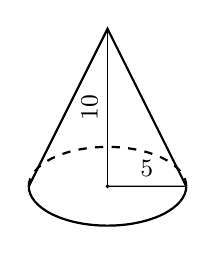
\begin{tikzpicture}[scale=.5]
\begin{scope}[xscale=2]
%\draw [thick](0,0) circle (1);
\draw [thick] (-1,0) arc (180:360:1);
\draw [thick,dashed] (1,0) arc (0:180:1);
\end{scope}

\draw [fill=black] (0,0) circle (1pt) -- node [pos=.5,above] {\small 5} (2,0);
\draw (0,0) -- node [pos=.5,rotate=90,above] {\small 10} (0,4);
\draw [thick] (-2,0) -- (0,4)-- (2,0);
\end{tikzpicture}

\item A skew right circular cone with height of 10 and base radius of 5. (Hint: all cross-sections are circles.)

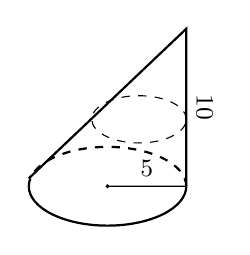
\begin{tikzpicture}[scale=.5]
\begin{scope}[xscale=2]
%\draw [thick](0,0) circle (1);
\draw [thick] (-1,0) arc (180:360:1);
\draw [thick,dashed] (1,0) arc (0:180:1);
\draw [dashed] (.4,1.7) circle (.6);
\end{scope}

\draw [fill=black] (0,0) circle (1pt) -- node [pos=.5,above] {\small 5} (2,0);
%\draw (0,0) -- node [pos=.5,rotate=90,above] {\small 10} (0,4);
\draw [thick] (-2,0.2) -- (2,4)-- node [pos=.5,rotate=-90,above] {\small 10}(2,0);
\end{tikzpicture}

\item A right triangular cone with height of 10 and whose base is a right, isosceles triangle with side length 4.

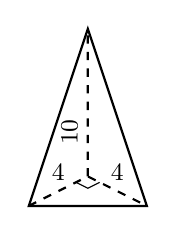
\begin{tikzpicture}[scale=.75]
\draw [thick](-1,0) -- (1,0) -- (0,3)--cycle;
\draw [thick,dashed] (-1,0) --  node [pos=.5,above] {\small 4} (0,.5) -- node [pos=.5,above] {\small 4} (1,0)
											(0,.5)-- node [pos=.3,above,rotate=90] {\small 10} (0,3);
\draw (-.2,.4) -- (0,.3) -- (.2,.4);
\end{tikzpicture}

\item A solid with length 10 with a rectangular base and triangular top, wherein one end is a square with side length 5 and the other end is a triangle with base and height of 5.

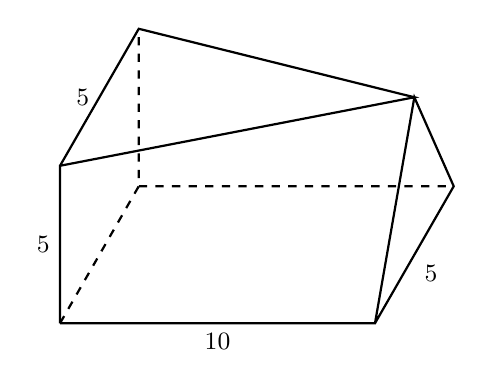
\begin{tikzpicture}[x={(1,0)},z={(0,1)},y={(.5,.87)},scale=.4]

\draw [thick] (0,0,0) -- node[pos=.5,below] {\small 10} (10,0,0) -- (10,2.5,5) -- (10,5,0) -- node [pos=.5,below right] {\small 5} (10,0,0)
							(0,0,0) -- node [pos=.5,left] {\small 5} (0,0,5) -- (10,2.5,5) -- (0,5,5) -- node [pos=.5,left] {\small 5} (0,0,5);
							
\draw [thick,dashed] (0,0,0) -- (0,5,0) -- (0,5,5)
										(0,5,0) -- (10,5,0);



\end{tikzpicture}

\end{enumerate}

%---------------------------------------------
% END OF EXERCISES ON SECOND PAGE
%---------------------------------------------
\end{multicols*}
\end{adjustwidth*}

\afterexercises 

\cleardoublepage
\section{Volume by The Shell Method} \label{S:6.2.ShellMethod}

\begin{goals}
\item Is there other methods to use a definite integral to find the volume of a three-dimensional solid  or a solid of revolution that results from revolving a two-dimensional region about a particular axis? 
\item In what circumstances do we integrate with respect to $y$ instead of integrating with respect to $x$?
\item When is it better to use the Shell Method as oppossed to the Washer Method? 
\end{goals}

%-------------------------------
% SUBSECTION INTRODUCTION
%-------------------------------
\subsection*{Introduction}

Often a given problem can be solved in more than one way. A particular method may be chosen out of convenience, personal preference, or perhaps necessity. Ultimately, it is good to have options.

The previous section introduced the Disk and Washer Methods, which computed the volume of solids of revolution by integrating the cross-sectional area of the solid. This section develops another method of computing volume, the \textbf{Shell Method.} Instead of slicing the solid perpendicular to the axis of rotation creating cross-sections, we now slice it parallel to the axis of rotation, creating ``shells.''

The Preview Activity \ref{PA:6.2} introduces a situation where using the Washer Method from Section \ref{S:6.1.Volume} becomes very tedious. 

\begin{marginfigure}[8cm] % MARGIN FIGURE
\margingraphics{figs/6/PA62.pdf}
\caption{The circular cone described in Preview Activity~\ref{PA:6.2}} \label{F:PA.6.2}
\end{marginfigure}

\begin{pa} \label{PA:6.2}  Consider the function $f(x)=x^2-x^3$, whose graph is in Figure~\ref{F:PA.6.2}.  Our goal in this activity is to use a definite integral to determine the volume of the solid formed by revolving the region bounded by $f(x)$ and $y=0$ about the $y$-axis.

\ba
\item Using the Washer Method, find an expression for the inner and outer radii of a slice.
\item Set up a definite integral to find the volume. If you try to evaluate the integral, what do you notice that happens? 
\item Find where the local maximum occurs.  
\item Use the results of past c) to split the solid into two pieces. Set up two definite integrals to find the volume of the original solid.  
	
\ea
\end{pa} 
\afterpa % PREVIEW need use f=x^2-x^3 and have do disk method

Consider Figure~\ref{fig:6.2.shell}-(a), where the region shown rotated around the $y$-axis forming the solid shown in Figure~\ref{fig:6.2.shell}-(b). A small slice of the region is drawn in Figure~\ref{fig:6.2.shell}-(a), parallel to the axis of rotation. When the region is rotated, this thin slice forms a \textbf{cylindrical shell}, as pictured in Figure~\ref{fig:6.2.shell}-(c). The previous section approximated a solid with lots of thin disks (or washers); we now approximate a solid with many thin cylindrical shells. 

To compute the volume of one shell, first consider the paper label on a soup can with radius $r$ and height $h$. What is the area of this label? A simple way of determining this is to cut the label and lay it out flat, forming a rectangle with height $h$ and length $2\pi r$. Thus the area is $A = 2\pi rh$; see Figure~\ref{F:6.2.soupcan}-(a).

\begin{marginfigure}[-1cm] % MARGIN FIGURE
\begin{center}
\subfloat[]{\includegraphics[scale=.95]{figures/figshell_intro_b}}

\subfloat[]{\includegraphics[scale=.95]{figures/figshell_intro_a}}

\subfloat[]{\includegraphics[scale=.95]{figures/figshell_intro_d}}
\caption{Introducing the Shell Method.}\label{fig:6.2.shell}
\end{center}
\end{marginfigure}

Do a similar process with a cylindrical shell, with height $h$, thickness $\Delta x$, and approximate radius $r$. Cutting the shell and laying it flat forms a rectangular solid with length $2\pi r$, height $h$ and depth $\dx$. Thus the volume is $V \approx 2\pi rh\dx$; see Figure~\ref{F:6.2.soupcan}-(b). (We say ``approximately'' since our radius was an approximation.)

By breaking the solid into $n$ cylindrical shells, we can approximate the volume of the solid as
$$V = \sum_{i=1}^n 2\pi r_ih_i\dx_i,$$ where $r_i$, $h_i$ and $\dx_i$ are the radius, height and thickness of the $i\,^\text{th}$ shell, respectively. 

This is a Riemann Sum. Taking a limit as the thickness of the shells approaches $0$ leads to a definite integral.

\begin{marginfigure}[1cm] % MARGIN FIGURE
\subfloat[]{\margingraphics{figures/figshell_soupcan}}

\subfloat[]{\margingraphics{figures/figshell_unwrapshell}}
\caption{Determining the volume of a thin cylindrical shell.}\label{F:6.2.soupcan}
\end{marginfigure}

\concept{The Shell Method} % CONCEPT
{Let a solid be formed by revolving a region $R$, bounded by $x=a$ and $x=b$, around a vertical axis. Let $r(x)$ represent the distance from the axis of rotation to $x$ (i.e., the radius of a sample shell) and let $h(x)$ represent the height of the solid at $x$ (i.e., the height of the shell). The volume of the solid is 
\index{integration!volume!Shell Method}\index{Shell Method}
$$V = 2\pi\int_a^b r(x)h(x)\ dx.$$
} %end CONCEPT

\textbf{Special Cases:}
\begin{enumerate}[1)]
\item When the region $R$ is bounded above by $y=f(x)$ and below by $y=g(x)$, then $h(x) = f(x)-g(x)$.
\item	When the axis of rotation is the $y$-axis (i.e., $x=0$) then $r(x) = x$.
\end{enumerate}
	
Let's practice using the Shell Method.

\begin{example} \label{eg:6.2.1} % EXAMPLE
Find the volume of the solid formed by rotating the region bounded by $y=0$, $y=1/(1+x^2)$, $x=0$ and $x=1$ about the $y$-axis.

\solution This is the region used to introduce the Shell Method in Figure~\ref{fig:6.2.shell}, but is sketched again in Figure~\ref{F:6.2.Ex1} for closer reference. A line is drawn in the region parallel to the axis of rotation representing a shell that will be carved out as the region is rotated about the $y$-axis. (This is the differential element.)

The distance this line is from the axis of rotation determines $r(x)$; as the distance from $x$ to the $y$-axis is $x$, we have $r(x)=x$. The height of this line determines $h(x)$; the top of the line is at $y=1/(1+x^2)$, whereas the bottom of the line is at $y=0$. Thus $h(x) = 1/(1+x^2)-0 = 1/(1+x^2)$. The region is bounded from $x=0$ to $x=1$, so the volume is 
\begin{align*}
V 	&= 2\pi\int_0^1 \frac{x}{1+x^2}\ dx. \\
\intertext{This requires substitution. Let $u=1+x^2$, so $du = 2x\ dx$. We also change the bounds: $u(0) = 1$ and $u(1) = 2$. Thus we have:}
&= \pi\int_1^2 \frac{1}{u}\ du \\
&= \pi\ln u\Big|_1^2\\
&= \pi\ln 2 \approx 2.178 \ \text{units}^3.
\end{align*}
Note: in order to find this volume using the Disk Method, two integrals would be needed to account for the regions above and below $y=1/2$.
\end{example}

\begin{marginfigure}[-14cm] %MARGIN FIGURE
\margingraphics{figures/figshell1}
\caption{Graphing a region in Example~\ref{eg:6.2.1}.} \label{F:6.2.Ex1}
\end{marginfigure} % EXAMPLE

With the Shell Method, nothing special needs to be accounted for to compute the volume of a solid that has a hole in the middle, as demonstrated next.

\begin{marginfigure}[2cm] %MARGIN FIGURE
\includegraphics{figures/figshell2a}
\caption{Graphing a region in Example~\ref{eg:6.2.2}.} \label{F:6.2.Ex2a}
\end{marginfigure}

\begin{example} \label{eg:6.2.2} % EXAMPLE
Find the volume of the solid formed by rotating the triangular region determined by the points $(0,1)$, $(1,1)$ and $(1,3)$ about the line $x=3$.

\solution
The region is sketched in Figure \ref{F:6.2.Ex2a} along with the differential element, a line within the region parallel to the axis of rotation. 

The height of the differential element is the distance from $y=1$ to $y=2x+1$, the line that connects the points $(0,1)$ and $(1,3)$. Thus $h(x) = 2x+1-1 = 2x$. The radius of the shell formed by the differential element is the distance from $x$ to $x=3$; that is, it is $r(x)=3-x$. The $x$-bounds of the region are $x=0$ to $x=1$, giving
\begin{align*}
V &=	2\pi\int_0^1 (3-x)(2x)\ dx \\
	&= 2\pi\int_0^1 \big(6x-2x^2)\ dx \\
	&= 2\pi\left(3x^2-\frac23x^3\right)\Big|_0^1\\
	&= \frac{14}{3}\pi\approx 14.66 \ \text{units}^3.
\end{align*}
\end{example}

\begin{marginfigure}[-5cm] %MARGIN FIGURE
\includegraphics{figures/figshell2b}
\caption{Graphing a region in Example~\ref{eg:6.2.2}.} \label{F:6.2.Ex2b}
\end{marginfigure} % EXAMPLE

\begin{activity} \label{A:6.2.1}  
In each of the following questions, draw a careful, labeled sketch of the region described, as well as the resulting solid that results from revolving the region about the stated axis.  In addition, draw a representative slice and state the volume of that slice, along with a definite integral whose value is the volume of the entire solid.  It is not necessary to evaluate the integrals you find.
\ba
	\item The region $S$ bounded by the $y$-axis, the curve $y = \sqrt{x}$, and the line $y = 2$; revolve $S$ about the $y$-axis.
	\item The region $S$ bounded by the $x$-axis, the curve $y = \sqrt{x}$, and the line $x = 4$; revolve $S$ about the $y$-axis.
	\item The finite region $S$ in the first quadrant bounded by the curves $y = 2x$ and $y = x^3$; revolve $S$ about the $y$-axis.
	\item The finite region $S$ bounded by the curves $x = (y-1)^2$ and $y  = x-1$; revolve $S$ about the $y$-axis.
	\item How do you answers to this activity compare to the results of Activty \ref{A:6.1.2}?
\ea

\end{activity}
\begin{smallhint}
\ba
	\item Small hints for each of the prompts above.
\ea
\end{smallhint}
\begin{bighint}
\ba
	\item Big hints for each of the prompts above.
\ea
\end{bighint}
\begin{activitySolution}
\ba
	\item Solutions for each of the prompts above.
\ea
\end{activitySolution}
\aftera
 % ACTIVITY

When revolving a region around a horizontal axis, we must consider the radius and height functions in terms of $y$, not $x$.

\begin{marginfigure}[6cm] %MARGIN FIGURE
\includegraphics{figures/figshell3a}
\caption{Graphing a region in Example~\ref{eg:6.2.3}.} \label{F:6.2.Ex3a}
\end{marginfigure}

\begin{example} \label{eg:6.2.3} % EXAMPLE
Find the volume of the solid formed by rotating the region given in Example~\ref{eg:6.2.2} about the $x$-axis.

\solution
The region is sketched in Figure~\ref{F:6.2.Ex3a} with a sample differential element and the solid is sketched in Figure~\ref{F:6.2.Ex3b}. (Note that the region looks slightly different than it did in the previous example as the bounds on the graph have changed.)

The height of the differential element is an $x$-distance, between $x=\frac12y-\frac12$ and $x=1$. Thus $h(y) = 1-(\frac12y-\frac12) = -\frac12y+\frac32.$ The radius is the distance from $y$ to the $x$-axis, so $r(y) =y$. The $y$ bounds of the region are $y=1$ and $y=3$, leading to the integral

\begin{align*}
V &= 2\pi\int_1^3\left[y\left(-\frac12y+\frac32\right)\right]\ dy \\
	&= 2\pi\int_1^3\left[-\frac12y^2+\frac32y\right]\ dy \\
	&= 2\pi\left[-\frac16y^3+\frac34y^2\right]\Big|_1^3 \\
	&= 2\pi\left[\frac94-\frac7{12}\right]\\
	&=	\frac{10}{3}\pi \approx 10.472\ \text{units}^3.
\end{align*}
\end{example}

\begin{marginfigure}[-6cm] %MARGIN FIGURE
\includegraphics{figures/figshell3b}
\caption{Graphing a region in Example~\ref{eg:6.2.3}.} \label{F:6.2.Ex3b}
\end{marginfigure} % EXAMPLE

\begin{activity} \label{A:6.2.2}  
In each of the following questions, draw a careful, labeled sketch of the region described, as well as the resulting solid that results from revolving the region about the stated axis.  In addition, draw a representative slice and state the volume of that slice, along with a definite integral whose value is the volume of the entire solid.  It is not necessary to evaluate the integrals you find.
\ba
	\item The region $S$ bounded by the $y$-axis, the curve $y = \sqrt{x}$, and the line $y = 2$; revolve $S$ about the $y$-axis.
	\item The region $S$ bounded by the $x$-axis, the curve $y = \sqrt{x}$, and the line $x = 4$; revolve $S$ about the $y$-axis.
	\item The finite region $S$ in the first quadrant bounded by the curves $y = 2x$ and $y = x^3$; revolve $S$ about the $x$-axis.	
	\item The finite region $S$ in the first quadrant bounded by the curves $y = 2x$ and $y = x^3$; revolve $S$ about the $y$-axis.
	\item The finite region $S$ bounded by the curves $x = (y-1)^2$ and $y  = x-1$; revolve $S$ about the $y$-axis
\ea

\end{activity}
\begin{smallhint}
\ba
	\item Small hints for each of the prompts above.
\ea
\end{smallhint}
\begin{bighint}
\ba
	\item Big hints for each of the prompts above.
\ea
\end{bighint}
\begin{activitySolution}
\ba
	\item Solutions for each of the prompts above.
\ea
\end{activitySolution}
\aftera
 % ACTIVITY

At the beginning of this section it was stated that ``it is good to have options.'' The next example finds the volume of a solid rather easily with the Shell Method, but using the Washer Method would be quite a chore.

\begin{marginfigure}[7cm] %MARGIN FIGURE
\includegraphics{figures/figshell4a}
\caption{Graphing a region in Example~\ref{eg:6.2.4}.} \label{F:6.2.Ex4a}
\end{marginfigure}

\begin{example} \label{eg:6.2.4} % EXAMPLE
Find the volume of the solid formed by revolving the region bounded by $y= \sin(x)$ and the $x$-axis from $x=0$ to $x=\pi$ about the $y$-axis.

\solution
The region and the resulting solid are given in Figure~\ref{F:6.2.Ex4a} and Figure~\ref{F:6.2.Ex4b} respectively.

The radius of a sample shell is $r(x) = x$; the height of a sample shell is $h(x) = \sin(x)$, each from $x=0$ to $x=\pi$. Thus the volume of the solid is 
\begin{align*}
V &=	2\pi\int_0^{\pi} x\sin(x)\ dx. \\
\intertext{This requires Integration By Parts. Set $u=x$ and $dv=\sin(x)\ dx$; we leave it to the reader to fill in the rest. We have:}
	&= 2\pi\Big[-x\cos(x)\Big|_0^{\pi} +\int_0^{\pi}\cos(x)\ dx \Big] \\
	&= 2\pi\Big[\pi + \sin(x) \Big|_0^{\pi}\ \Big] \\
	&= 2\pi\Big[\pi + 0 \Big] \\
	&= 2\pi^2 \approx 19.74 \ \text{units}^3.
	\end{align*}

Note that in order to use the Washer Method, we would need to solve $y=\sin(x)$ for $x$, requiring the use of the arcsine function. We leave it to the reader to verify that the outside radius function is $R(y) = \pi-\arcsin(y)$ and the inside radius function is $r(y)=\arcsin(y)$. Thus the volume can be computed as $$\pi\int_0^1 \Big[ (\pi-\arcsin(y))^2-(\arcsin(y))^2\Big]\ dy.$$	This integral isn't terrible given that the $\arcsin^2(y)$ terms cancel, but it is more onerous than the integral created by the Shell Method.
\end{example}

\begin{marginfigure}[-8cm] %MARGIN FIGURE
\includegraphics{figures/figshell4b}
\caption{Graphing a region in Example~\ref{eg:6.2.4}.} \label{F:6.2.Ex4b}
\end{marginfigure} % EXAMPLE

%--------------------------------------------
% SUMMARY
%--------------------------------------------
\begin{summary}
  \item We can use a definite integral to find the volume of a three-dimensional solid of revolution that results from revolving a two-dimensional region about a particular axis by taking  slices parallel to the axis of revolution which will then be cylindrical shells.
  \item If we revolve about a vertical line and slice perpendicular to that line, then our shells are vertical and of thickness $\triangle x$. This leads us to integrate with respect to $x$.
	\item If we revolve about a horizontal line and slice parallel to that line, then our shells are horizontal and of thickness $\triangle y$. This leads us to integrate with respect to $y$, as opposed to with respect to $x$ when we slice a solid vertically.
	\item Let a region $R$ be given with $x$-bounds $x=a$ and $x=b$ and $y$-bounds $y=c$ and $y=d$.
\vskip 5pt
\begin{tabular}{cccc}
 		& Washer Method & & Shell Method \rule[-10pt]{0pt}{10pt} \\
 \parbox{50pt}{\centering Horizontal Axis}  & $\ds \pi\int_a^b \big(R(x)^2-r(x)^2\big)\ dx$ & & $\ds 2\pi\int_c^d r(y)h(y)\ dy$ \\ \\
 \parbox{40pt}{\centering Vertical Axis} &  $\ds\pi \int_c^d\big(R(y)^2-r(y)^2\big)\ dy$ & & $\ds 2\pi\int_a^b r(x)h(x)\ dx$
 \end{tabular}
\index{integration!volume!Washer Method}\index{Washer Method}\index{integration!volume!Shell Method}\index{Shell Method}
\end{summary} 

\clearpage

%--------------
% EXERCISES
%--------------
\begin{adjustwidth*}{}{-2.25in}
\textbf{{\large Exercises}}
\setlength{\columnsep}{25pt}
\begin{multicols*}{2}
\noindent Terms and Concepts \small
\begin{enumerate}[1)]
\item T/F: A solid of revolution is formed by revolving a shape around an axis.
\item T/F: The Shell Method can only be used when the Washer Method fails.
\item T/F: The Shell Method works by integrating cross--sectional areas of a solid.
\item T/F: When finding the volume of a solid of revolution that was revolved around a vertical axis, the Shell Method integrates
with respect to $x$.
\end{enumerate} 

\noindent {\normalsize Problems} \small

\noindent{\bf In Exercises 5--8, a region of the Cartesian plane is shaded. Use the Shell Method to find the volume of the solid of revolution formed by revolving the region about the $y$-axis.}

\begin{enumerate}[1),resume]
\item \begin{minipage}{\linewidth}\centering\includegraphics{figures/fig07_02_ex_09}\end{minipage}
\item \begin{minipage}{\linewidth}\centering\includegraphics{figures/fig07_02_ex_06}\end{minipage}
\item \begin{minipage}{\linewidth}\centering\includegraphics{figures/fig07_02_ex_07}\end{minipage}
\item \begin{minipage}{\linewidth}\centering\includegraphics{figures/fig07_02_ex_04}\end{minipage}

%\item \begin{minipage}{\linewidth}\centering\includegraphics{figures/fig07_02_ex_05}\end{minipage}
\end{enumerate}

\noindent{\bf In Exercises 9--12, a region of the Cartesian plane is shaded. Use the Shell Method to find the volume of the solid of revolution formed by revolving the region about the $x$-axis.}

\begin{enumerate}[1),resume]
\item \begin{minipage}{\linewidth}\centering\includegraphics{figures/fig07_02_ex_05}\end{minipage}
\item \begin{minipage}{\linewidth}\centering\includegraphics{figures/fig07_02_ex_10}\end{minipage}
\item \begin{minipage}{\linewidth}\centering\includegraphics{figures/fig07_02_ex_07}\end{minipage}
\end{enumerate}

%------------------------------------------
% END OF EXERCISES ON FIRST PAGE
%------------------------------------------
\end{multicols*}
\end{adjustwidth*}

\clearpage

\begin{adjustwidth*}{}{-2.25in}
\setlength{\columnsep}{25pt}
\begin{multicols*}{2}\small

\begin{enumerate}[1),start=12]
\item \begin{minipage}{\linewidth}\centering\includegraphics{figures/fig07_02_ex_04}\end{minipage}
\end{enumerate}

\vspace{.25cm}

\noindent{\bf In Exercises 13--18, a region of the Cartesian plane is described. Use the Shell Method to find the volume of the solid of revolution formed by rotating the region about each of the given axes.}

\begin{enumerate}[1),resume]
\item Region bounded by: $y=\sqrt{x}$, $y=0$ and $x=1$.

Rotate about:

\noindent%
\begin{minipage}[t]{.5\linewidth}
\begin{enumerate}
\item		the $y$-axis
\item		$x=1$
\end{enumerate}
\end{minipage}
\begin{minipage}[t]{.5\linewidth}
\begin{enumerate}\addtocounter{enumii}{2}
\item		the $x$-axis
\item		$y=1$
\end{enumerate}
\end{minipage}

\item Region bounded by: $y=4-x^2$ and $y=0$.

Rotate about:

\noindent%
\begin{minipage}[t]{.5\linewidth}
\begin{enumerate}
\item		$x=2$
\item		$x=-2$
\end{enumerate}
\end{minipage}
\begin{minipage}[t]{.5\linewidth}
\begin{enumerate}\addtocounter{enumii}{2}
\item		the $x$-axis
\item		$y=4$
\end{enumerate}
\end{minipage}

\item The triangle with vertices $(1,1)$, $(1,2)$ and $(2,1)$.

Rotate about:

\noindent%
\begin{minipage}[t]{.5\linewidth}
\begin{enumerate}
\item		the $y$-axis
\item		$x=1$
\end{enumerate}
\end{minipage}
\begin{minipage}[t]{.5\linewidth}
\begin{enumerate}\addtocounter{enumii}{2}
\item		the $x$-axis
\item		$y=2$
\end{enumerate}
\end{minipage}

\item Region bounded by $y=x^2-2x+2$ and $y=2x-1$.

Rotate about:

\noindent%
\begin{minipage}[t]{.5\linewidth}
\begin{enumerate}
\item		the $y$-axis
\item		$x=1$
\end{enumerate}
\end{minipage}
\begin{minipage}[t]{.5\linewidth}
\begin{enumerate}\addtocounter{enumii}{2}
%\item		the $y$-axis
\item		$x=-1$
\end{enumerate}
\end{minipage}

\item Region bounded by $y=1/\sqrt{x^2+1}$, $x=-1$, $x=1$ and the $x$-axis.

Rotate about:

\noindent%
\begin{minipage}[t]{.5\linewidth}
\begin{enumerate}
\item		the $y$-axis
\item		$x=1$
\end{enumerate}
\end{minipage}
\begin{minipage}[t]{.5\linewidth}
\begin{enumerate}\addtocounter{enumii}{2}
%\item		the $y$-axis
\item		$y=-1$
\end{enumerate}
\end{minipage}

\item Region bounded by $y=2x$, $y=x$ and $x=2$.

Rotate about:

\noindent%
\begin{minipage}[t]{.5\linewidth}
\begin{enumerate}
\item		the $y$-axis
\item		$x=2$
\end{enumerate}
\end{minipage}
\begin{minipage}[t]{.5\linewidth}
\begin{enumerate}\addtocounter{enumii}{2}
\item		the $x$-axis
\item		$y=4$
\end{enumerate}
\end{minipage}

\end{enumerate}

%---------------------------------------------
% END OF EXERCISES ON SECOND PAGE
%---------------------------------------------
\end{multicols*}
\end{adjustwidth*}

\afterexercises 

\cleardoublepage
\section{Arc Length and Surface Area} \label{S:6.3.ArcLength}

\begin{goals}
\item How can a definite integral be used to measure the length of a curve?
\item How can a definite integral be used to measure the surface area of a solid of revolution?
\end{goals}

%-------------------------------
% SUBSECTION INTRODUCTION
%-------------------------------
\subsection*{Introduction}

\begin{marginfigure}[6cm] % MARGIN FIGURE
\margingraphics{figures/6_1_Intro.eps}
\caption{The area between a nonnegative function $f$ and the $x$-axis on the interval $[a,b]$.} \label{F:6.1.Intro}
\end{marginfigure}

Early on in our work with the definite integral, we learned that if we have a nonnegative velocity function, $v$, for an object moving along an axis, the area under the velocity function between $a$ and $b$ tells us the distance the object traveled on that time interval.  Moreover, based on the definition of the definite integral, that area is given precisely by $\int_a^b v(t) \, dt$.  Indeed, for any nonnegative function $f$ on an interval $[a,b]$, we know that $\int_a^b f(x) \, dx$ measures the area bounded by the curve and the $x$-axis between $x = a$ and $x = b$, as shown in Figure~\ref{F:6.1.Intro}.

Through our upcoming work in the present section and chapter, we will explore how definite integrals can be used to represent a variety of different physically important properties.  In Preview Activity~\ref{PA:6.1}, we begin this investigation by seeing how a single definite integral may be used to represent the area between two curves.

\begin{pa} \label{PA:6.3}  In the following, we consider the function $f(x)=1-x^2$ over the interval $[-1,1]$. Our goal is to estimate the length of the curve. 

\ba
\item Graph $f(x)$ over the interval $[-1,1]$. Label the points on the curve that correspond to $x=-1,-\frac12,0,1/2$, and $1$.  

\item Draw the secant line connecting the points $(-1,f(-1)$ and \newline $(-\frac{1}{2},f(-\frac{1}{2}))$. Use the distance formula to find the length of the secant line from $x=-1$ to $x=-\frac12$.
\item Repeat drawing a secant line between the remaining points starting with $(-\frac{1}{2},f(-\frac{1}{2}))$ and $(0,f(0))$. For each line segment , use the distance formula to find the length of the segment.
\item Add the distances together to get an approximation to the length of the curve. 
\item How can we improve our approximation? Write a Riemann sum that will give an improvement to our approximation. 
\ea
\end{pa} 
\afterpa % PREVIEW 

%------------------------------------------
% SUBSECTION FINDING THE LENGTH OF A CURVE
%------------------------------------------
\subsection*{Finding the length of a curve} \index{arc length}

In addition to being able to use definite integrals to find the volumes of solids of revolution, we can also use the definite integral to find the length of a portion of a curve.  We use the same fundamental principle:  we take a curve whose length we cannot easily find, and slice it up into small pieces whose lengths we can easily approximate.  In particular, we take a given curve and subdivide it into small approximating line segments, as shown at left in Figure~\ref{F:6.3.ArcLength}.
  
\begin{marginfigure}[2cm] % MARGIN FIGURE
\margingraphics{figures/6_1_ArcLength.eps}
\caption{At left, a continuous function $y = f(x)$ whose length we seek on the interval $a = x_0$ to $b = x_3$.  At right, a close up view of a portion of the curve.} \label{F:6.3.ArcLength}
\end{marginfigure}

To see how we find such a definite integral that measures arc length on the curve $y = f(x)$ from $x = a$ to $x = b$, we think about the portion of length, $L_{\mbox{\small{slice}}}$, that lies along the curve on a small interval of length $\triangle x$, and estimate the value of $L{\mbox{\small{slice}}}$ using a well-chosen triangle.  In particular, if we consider the right triangle with legs parallel to the coordinate axes and hypotenuse connecting two points on the curve, as seen at right in Figure~\ref{F:6.3.ArcLength}, we see that the length, $h$, of the hypotenuse approximates the length, $L_{\mbox{\small{slice}}}$, of the curve between the two selected points.  Thus,
$$L_{\mbox{\small{slice}}} \approx h = \sqrt{ (\triangle x)^2 + (\triangle y)^2 }.$$
By algebraically rearranging the expression for the length of the hypotenuse, we see how a definite integral can be used to compute the length of a curve.  In particular, observe that by removing a factor of $(\triangle x)^2$, we find that
\begin{eqnarray*}
L_{\mbox{\small{slice}}} & \approx & \sqrt{ (\triangle x)^2 + (\triangle y)^2 } \\
& = & \sqrt{ (\triangle x)^2\left(1 + \frac{(\triangle y)^2}{(\triangle x)^2} \right)} \\
& = & \sqrt{1 + \frac{(\triangle y)^2}{(\triangle x)^2} } \cdot \triangle x.
\end{eqnarray*}
Furthermore, as $n \to \infty$ and $\triangle x \to 0$, it follows that $\frac{\triangle y}{\triangle x} \to \frac{dy}{dx} = f'(x)$.  Thus, we can say that
$$L_{\mbox{\small{slice}}} \approx \sqrt{1 + f'(x)^2} \triangle x.$$
Taking a Riemann sum of all of these slices and letting $n \to \infty$, we arrive at the following fact.

\concept{Arc Length}{ %CONCEPT
Given a differentiable function $f$ on an interval $[a,b]$, the total arc length\index{arc length}, $L$, along the curve $y = f(x)$ from $x = a$ to $x = b$ is given by
$$L = \int_a^b \sqrt{1+f'(x)^2} \, dx.$$
} %end CONCEPT

\begin{example} \label{eg:6.3.1} % EXAMPLE
Find the arc length of $f(x) = x^{3/2}$ from $x=0$ to $x=4$. 

\solution
We begin by finding $\fp(x)= \frac32x^{1/2}$. Using the formula, we find the arc length $L$ as
\begin{align*}
	L &=	\int_0^4 \sqrt{1+\left(\frac32x^{1/2}\right)^2}\ dx \\
		&=	\int_0^4 \sqrt{1+\frac94x} \ dx \\
		&= 	\int_0^4 \left(1+\frac94x\right)^{1/2}\ dx \\
		&=  \frac23\frac49\left(1+\frac94x\right)^{3/2}\Big|_0^4 \\
		&=\frac{8}{27}\left(10^{3/2}-1\right) \approx 9.07 \text{units}.
\end{align*}
A graph of $f$ is given in Figure \ref{F:6.3.Ex1}.
\end{example}

\begin{marginfigure}[-8cm] %MARGIN FIGURE
\includegraphics{figures/figarc1}
\caption{A graph of $f(x) = x^{3/2}$ from Example~\ref{eg:6.3.1}.} \label{F:6.3.Ex1}
\end{marginfigure}

 % EXAMPLE

\begin{example} \label{eg:6.3.2} % EXAMPLE
Find the arc length of $\ds f(x) =\frac18x^2-\ln x$ from $x=1$ to $x=2$.

\solution
This function was chosen specifically because the resulting integral can be evaluated exactly. We begin by finding $\fp(x) = x/4-1/x$. The arc length is 
\begin{align*}
L		&=  \int_1^2 \sqrt{1+ \left(\frac x4-\frac1x\right)^2}\ dx \\
		&= 	\int_1^2 \sqrt{1 + \frac{x^2}{16} -\frac12 + \frac1{x^2} } \ dx \\
\end{align*}
\begin{align*}
\phantom{L}
		&=	\int_1^2 \sqrt{\frac{x^2}{16} +\frac12 + \frac1{x^2} } \ dx \\
		&=	\int_1^2	\sqrt{ \left(\frac x4 + \frac1x\right)^2}\ dx \\
		&= \int_1^2 \left(\frac x4 + \frac1x\right) \ dx \\
		&=  \left(\frac{x^2}8 + \ln x\right)\Bigg|_1^2\\
		&=	\frac38+\ln 2 \approx 1.07 \ \text{units}.
\end{align*}
	
A graph of $f$ is given in Figure \ref{F:6.3.Ex2}; the portion of the curve measured in this problem is in bold.

\end{example}

\begin{marginfigure}[-8cm] %MARGIN FIGURE
\includegraphics{figures/figarc1}
\caption{A graph of $f(x) = \frac18x^2-\ln x$ from Example~\ref{eg:6.3.2}.} \label{F:6.3.Ex2}
\end{marginfigure}

 % EXAMPLE

\begin{margintable}[3cm]
\begin{center}
\scalebox{1.15}{
\begin{tabular}{c | r} 
 $x$ & $\sqrt{1+\cos^2x}$ \\ \hline
 $0$ & $\sqrt{2}$ \\
 $\pi/4$ & $\sqrt{3/2}$ \\
 $\pi/2$ & $1$ \\
 $3 \pi/4$ & $\sqrt{3/2}$ \\
 $\pi$  & $\sqrt{2}$ \\
\end{tabular}}
\end{center}
\caption{A table of values of $y=\sqrt{1+\cos^2x}$ to evaluate a definite integral in Example \ref{eg:6.3.3}.} \label{T:6.3.Ex3}
\end{margintable}

\begin{example} \label{eg:6.3.3} % EXAMPLE
Find the length of the sine curve from $x=0$ to $x=\pi$.

\solution This is somewhat of a mathematical curiosity; in Activity \ref{A:4.5.1} (b) we found the area under one ``hump'' of the sine curve is 2 square units; now we are measuring its arc length.

The setup is straightforward: $f(x) = \sin x$ and $\fp(x) = \cos x$. Thus 
$$L = \int_0^\pi \sqrt{1+\cos^2x}\ dx.$$
This integral \textit{cannot} be evaluated in terms of elementary functions so we will approximate it with Simpson's Method with $n=4$. 

Table~\ref{T:6.3.Ex3} gives $\sqrt{1+\cos^2x}$ evaluated at 5 evenly spaced points in $[0,\pi]$. Simpson's Rule then states that 
\begin{align*}
\int_0^\pi \sqrt{1+\cos^2x}\ dx &\approx	\frac{\pi-0}{4\cdot 3}\left(\sqrt{2}+4\sqrt{3/2}+2(1)+4\sqrt{3/2}+\sqrt{2}\right) \\
			&=3.82918.
\end{align*}
Using a computer with $n=100$ the approximation is $L\approx 3.8202$; our approximation with $n=4$ is quite good.
\end{example} % EXAMPLE

\begin{activity} \label{A:6.3.1}  Each of the following questions somehow involves the arc length along a curve.
\ba
	
	\item Use the definition and appropriate computational technology to determine the arc length along $y = x^2$ from $x = -1$ to $x = 1$.
	\item Find the arc length of $y = \sqrt{4-x^2}$ on the interval $0 \le x \le 4$.  Find this value in two different ways: (a) by using a definite integral, and (b) by using a familiar property of the curve.
	\item Determine the arc length of $y = xe^{3x}$ on the interval $[0,1]$.
	\item Will the integrals that arise calculating arc length typically be ones that we can evaluate exactly using the First FTC, or ones that we need to approximate?  Why?
	\item A moving particle is traveling along the curve given by $y = f(x) = 0.1x^2 + 1$, and does so at a constant rate of 7 cm/sec, where both $x$ and $y$ are measured in cm (that is, the curve $y = f(x)$ is the path along which the object actually travels; the curve is not a ``position function'').  Find the position of the particle when $t = 4$ sec, assuming that when $t = 0$, the particle's location is $(0,f(0))$.
\ea

\end{activity}
\begin{smallhint}
\ba
	\item Small hints for each of the prompts above.
\ea
\end{smallhint}
\begin{bighint}
\ba
	\item Big hints for each of the prompts above.
\ea
\end{bighint}
\begin{activitySolution}
\ba
	\item Solutions for each of the prompts above.
\ea
\end{activitySolution}
\aftera % ACTIVITY

%-------------------------------------------------
% SUBSECTION SURFACE AREA OF SOLIDS OF REVOLUTION
%-------------------------------------------------
\subsection*{Surface Area of Solids of Revolution}

We have already seen how a curve $y=f(x)$ on $[a,b]$ can be revolved around an axis to form a solid. Instead of computing its volume, we now consider its surface area.

\begin{marginfigure}[6cm] % MARGIN FIGURE
\captionsetup[subfigure]{labelformat=empty}
\subfloat{\margingraphics{figures/figarc4b}}

\subfloat{\margingraphics{figures/figarc4}}

\caption{Establishing the formula for surface area.} \label{F:6-3_SurfArea}
\end{marginfigure}

We begin as we have in the previous sections: we partition the interval $[a,b]$ with $n$ subintervals, where the $i\,^{\text{th}}$ subinterval is $[x_i,x_{i+1}]$. On each subinterval, we can approximate the curve $y=f(x)$ with a straight line that connects $f(x_i)$ and $f(x_{i+1})$ as shown in Figure \ref{F:6-3_SurfArea} (a). Revolving this line segment about the $x$-axis creates part of a cone (called the \textit{frustum} of a cone) as shown in Figure \ref{F:6-3_SurfArea} (b). The surface area of a frustum of a cone is $$2\pi\cdot\text{ length }\cdot\text{average of the two radii $R$ and $r$}.$$

The length is given by $L$; we use the material just covered by arc length to state that $$L\approx \sqrt{1+\fp(c_i)}\dx_i$$ for some $c_i$ in the $i\,^\text{th}$ subinterval. The radii are just the function evaluated at the endpoints of the interval. That is, $$R = f(x_{i+1})\quad \text{and}\quad r = f(x_i).$$

Thus the surface area of this sample frustum of the cone is approximately 
$$2\pi\frac{f(x_i)+f(x_{i+1})}2\sqrt{1+\fp(c_i)^2}\dx_i.$$

Since $f$ is a continuous function, the Intermediate Value Theorem states there is some $d_i$ in $[x_i,x_{i+1}]$ such that \newline $\ds f(d_i) = \frac{f(x_i)+f(x_{i+1})}2$; we can use this to rewrite the above equation as
$$2\pi f(d_i)\sqrt{1+\fp(c_i)^2}\dx_i.$$
Summing over all the subintervals we get the total surface area to be approximately 
$$\text{Surface Area}\approx \sum_{i=1}^n 2\pi f(d_i)\sqrt{1+\fp(c_i)^2}\dx_i,$$
which is a Riemann Sum. Taking the limit as the subinterval lengths go to zero gives us the exact surface area, given in the following Key Idea.

\concept{Surface Area of a Solid of Revolution} %CONCEPT
{Let $f$ be differentiable on an open interval containing $[a,b]$ where $\fp$ is also continuous on $[a,b]$. \index{integration!surface area}\index{surface area!solid of revolution}
	\begin{enumerate}[1)]
	\item	The surface area of the solid formed by revolving the graph of $y=f(x)$, where $f(x)\geq0$, about the $x$-axis is
	$$\text{Surface Area} = 2\pi\int_a^b f(x)\sqrt{1+\fp(x)^2}\ dx.$$
	\item	The surface area of the solid formed by revolving the graph of $y=f(x)$ about the $y$-axis, where $a,b\geq0$, is
	$$\text{Surface Area} = 2\pi\int_a^b x\sqrt{1+\fp(x)^2}\ dx.$$
	\end{enumerate}
} %end CONCEPT

\marginnote{When revolving $y=f(x)$ about the $y$-axis, the radii of the resulting frustum are $x_i$ and $x_{i+1}$; their average value is simply the midpoint of the interval. In the limit, this midpoint is just $x$. }

\begin{example} \label{eg:6.3.4} % EXAMPLE
Find the surface area of the solid formed by revolving $y=\sin x$ on $[0,\pi]$ around the $x$-axis, as shown in Figure \ref{F:6.3.Ex4}.

\solution
The setup is relatively straightforward; we have the surface area $SA$ is:
\begin{align*}
SA  &=	2\pi\int_0^\pi \sin x\sqrt{1+\cos^2x}\ dx \\
	&= 2\pi \int_{-1}^1 \sqrt{1+u^2} \ du \\
		&=	2\pi \int_{-\pi/4}^{\pi/4} \sec^3\theta \ d\theta \\
		&= 2\pi\sqrt{2}.		
\end{align*}
The integration above is nontrivial, utilizing Substitution, Trigonometric Substitution, and Integration by Parts.
\end{example}

\begin{marginfigure}[-8cm] %MARGIN FIGURE
\includegraphics{figures/figsa1}
\caption{Revolving $y=\sin x$ on $[0,\pi]$ about the $x$-axis.} \label{F:6.3.Ex4}
\end{marginfigure}



 % EXAMPLE

\begin{example} \label{eg:6.3.5} % EXAMPLE
Find the surface area of the solid formed by revolving the curve $y=x^2$ on $[0,1]$ about:
\begin{enumerate}[1)]
\item the $x$-axis
\item	 the $y$-axis.
\end{enumerate}

\solution
\begin{enumerate}[1)]
\item The integral is straightforward to setup:
\begin{align*}
SA &= 2\pi\int_0^1 x^2\sqrt{1+(2x)^2}\ dx.
\intertext{Like the integral in Example \ref{eg:6.3.4}, this requires Trigonometric Substitution.}
&= \left.\frac{\pi}{32}\left(2(8x^3+x)\sqrt{1+4x^2}-\sinh^{-1}(2x)\right)\right|_0^1\\
&=\frac{\pi}{32}\left(18\sqrt{5}-\sinh^{-1}2\right)\\
&\approx 3.81\ \text{units}^2.
\end{align*}
The solid formed by revolving $y=x^2$ around the $x$-axis is graphed in Figure \ref{F:6.3.Ex5}-(a).
	
\item	 Since we are revolving around the $y$-axis, the ``radius'' of the solid is not $f(x)$ but rather $x$. Thus the integral to compute the surface area is:
\begin{align*}
SA &= 2\pi\int_0^1x\sqrt{1+(2x)^2}\ dx.
\intertext{This integral can be solved using substitution. Set $u=1+4x^2$; the new bounds are $u=1$ to $u=5$. We then have }
&=	\frac{\pi}4\int_1^5 \sqrt{u}\ du \\
&= \left.\frac{\pi}{4}\frac23 u^{3/2}\right|_1^5\\
&= \frac{\pi}6\left(5\sqrt{5}-1\right)\\
&\approx 5.33\ \text{units}^2.
\end{align*}
 The solid formed by revolving $y=x^2$ about the $y$-axis is graphed in Figure \ref{F:6.3.Ex5}-(b).	
\end{enumerate}
\end{example}

\begin{marginfigure}[-15cm] %MARGIN FIGURE
%\captionsetup[subfigure]{labelformat=empty}
\subfloat[]{\margingraphics{figures/figsa2a}}

\vspace{1cm}

\subfloat[]{\margingraphics{figures/figsa2b}}

\caption{The solids used in Example \ref{eg:6.3.5}} \label{F:6.3.Ex5}
\end{marginfigure}



 % EXAMPLE

This last example is a famous mathematical ``paradox.''

\begin{example} \label{eg:6.3.6} % EXAMPLE
%\textbf{The surface area and volume of Gabriel's Horn} 

Consider the solid formed by revolving $y=1/x$ about the $x$-axis on $[1,\infty)$. Find the volume and surface area of this solid. (This shape, as graphed in Figure \ref{F:6.3.Ex6}, is known as ``Gabriel's Horn'' since it looks like a very long horn that only a supernatural person, such as an angel, could play.)\index{Gabriel's Horn}

\solution
To compute the volume it is natural to use the Disk Method. We have:
\begin{align*}
V &= \pi\int_1^\infty \frac{1}{x^2}\ dx \\
	&= \lim_{b\to\infty}\pi\int_1^b\frac{1}{x^2}\ dx \\
	&=	\lim_{b\to\infty} \left.\pi\left(\frac{-1}{x}\right)\right|_1^b \\
	&= \lim_{b\to\infty} \pi\left(1-\frac1b\right) \\
	&= \pi \ \text{units}^3.
\end{align*}
Gabriel's Horn has a finite volume of $\pi$ cubic units. Since we have already seen that objects with infinite length can have a finite area, this is not too difficult to accept.

We now consider its surface area. The integral is straightforward to setup:
\begin{align*}
SA &= 2\pi\int_1^\infty \frac{1}{x}\sqrt{1+1/x^4}\ dx.
\intertext{Integrating this expression is not trivial. We can, however, compare it to other improper integrals. Since $1< \sqrt{1+1/x^4} $ on $[1,\infty)$, we can state that}
2\pi\int_1^\infty \frac{1}{x}\ dx &<2\pi\int_1^\infty \frac{1}{x}\sqrt{1+1/x^4}\ dx .
\end{align*}
The improper integral on the left diverges. Since the integral on the right is larger, we conclude it also diverges, meaning Gabriel's Horn has infinite surface area.

Hence the ``paradox'': we can fill Gabriel's Horn with a finite amount of paint, but since it has infinite surface area, we can never paint it.

Somehow this paradox is striking when we think about it in terms of volume and area. However, we have seen a similar paradox before, as referenced above. We know that the area under the curve $y=1/x^2$ on $[1,\infty)$ is finite, yet the shape has an infinite perimeter. Strange things can occur when we deal with the infinite.

\end{example}

\begin{marginfigure}[-8cm] %MARGIN FIGURE
\margingraphics{figures/figgabriel}
\caption{A graph of Gabriel's Horn.} \label{F:6.3.Ex6}
\end{marginfigure}



 % EXAMPLE

%--------------------------------------------
% SUMMARY
%--------------------------------------------
\begin{summary}
  \item To find the area between two curves, we think about slicing the region into thin rectangles.  If, for instance, the area of a typical rectangle on the interval $x = a$ to $x = b$ is given by $A_{\mbox{\small{rect}}} = (g(x) - f(x)) \triangle x,$ then the exact area of the region is given by the definite integral
  $$A = \int_a^b (g(x)-f(x))\, dx.$$
  \item The shape of the region usually dictates whether we should use vertical rectangles of thickness $\triangle x$ or horizontal rectangles of thickness $\triangle y$.  We desire to have the height of the rectangle governed by the difference between two curves:  if those curves are best thought of as functions of $y$, we use horizontal rectangles, whereas if those curves are best viewed as functions of $x$, we use vertical rectangles.
  \item The arc length, $L$, along the curve $y = f(x)$ from $x = a$ to $x = b$ is given by
$$L = \int_a^b \sqrt{1 + f'(x)^2} \, dx.$$
\end{summary}

\clearpage

%--------------
% EXERCISES
%--------------
\begin{adjustwidth*}{}{-2.25in}
\textbf{{\large Exercises}}
\setlength{\columnsep}{25pt}
\begin{multicols*}{2}
\noindent Terms and Concepts \small
\begin{enumerate}[1)]
\item T/F: The integral formula for computing Arc Length was found by first approximating arc length with straight line segments.
\item T/F: The integral formula for computing Arc Length includes a square--root, meaning the integration is probably easy.
\end{enumerate} 

\noindent {\normalsize Problems} \small

\noindent{\bf In Exercises 3--11, find the arc length of the function on the given integral.}

\begin{enumerate}[1),resume]
\item $\ds f(x) = x$ on $[0, 1]$
\item $\ds f(x) = \sqrt{8x}$ on $[-1, 1]$
\item $\ds f(x) = \frac13x^{3/2}-x^{1/2}$ on $[0,1]$
\item $\ds f(x) = \frac1{12}x^{3}+\frac1x$ on $[1,4]$
\item $\ds f(x) = 2x^{3/2}-\frac16\sqrt{x}$ on $[0,9]$
\item $\ds f(x) = \frac12\big(e^x+e^{-x}\big)$ on $[0, \ln 5]$
\item $\ds f(x) = \frac1{12}x^5+\frac1{5x^3}$ on $[.1, 1]$
\item $\ds f(x) = \ln \big(\sin x\big)$ on $[\pi/6, \pi/2]$
\item $\ds f(x) = \ln \big(\cos x\big)$ on $[0, \pi/4]$
\end{enumerate}

\noindent{\bf In Exercises 12--19, set up the integral to compute the arc length of the function on the given interval. Try to compute the integral by hand, and use a CAS to compute the integral.  Also, use Simpson's Rule with $n = 4$ to approximate the arc length.}

\begin{enumerate}[1),resume]
\item $\ds f(x) = x^2$ on $[0, 1]$.\label{ex_07_04_ex_13}
\item $\ds f(x) = x^{10}$ on $[0, 1]$
\item $\ds f(x) = \sqrt{x}$ on $[0, 1]$
\item $\ds f(x) = \ln x$ on $[1, e]$
\item $\ds f(x) = \sqrt{1-x^2}$ on $[-1, 1]$. (Note: this describes the top half of a circle with radius 1.)
\item $\ds f(x) = \sqrt{1-x^2/9}$ on $[-3, 3]$. (Note: this describes the top half of an ellipse with a major axis of length 6 and a minor axis of length 2.)
\item $\ds f(x) = \frac1x$ on $[1,2]$
\item $\ds f(x) = \sec x$ on $[-\pi/4,\pi/4]$.\label{ex_07_04_ex_20}
\end{enumerate}

\columnbreak

\noindent{\bf In Exercises 20--24, find the surface area of the described solid of revolution.}

\begin{enumerate}[1),resume]
\item The solid formed by revolving $y=2x$ on $[0,1]$ about the $x$-axis.
\item The solid formed by revolving $y=x^2$ on $[0,1]$ about the $y$-axis.
\item The solid formed by revolving $y=x^3$ on $[0,1]$ about the $x$-axis.
\item The solid formed by revolving $y=\sqrt{x}$ on $[0,1]$ about the $x$-axis.
\item The sphere formed by revolving $y=\sqrt{1-x^2}$ on $[-1,1]$ about the $x$-axis.
\end{enumerate}

%------------------------------------------
% END OF EXERCISES ON FIRST PAGE
%------------------------------------------
\end{multicols*}
\end{adjustwidth*}

%\clearpage
%
%\begin{adjustwidth*}{}{-2.25in}
%\setlength{\columnsep}{25pt}
%\begin{multicols*}{2}\small
%
%\begin{enumerate}[1),start=12]
%
%\end{enumerate}
%
%%---------------------------------------------
%% END OF EXERCISES ON SECOND PAGE
%%---------------------------------------------
%\end{multicols*}
%\end{adjustwidth*}

\afterexercises 

\cleardoublepage
\section{Density, Mass, and Center of Mass} \label{S:6.4.Mass}

\begin{goals}
\item How are mass, density, and volume related?  
\item How is the mass of an object with varying density computed?
\item What is the center of mass of an object, and how are definite integrals used to compute it?
\end{goals}

%-----------------------------------
% SUBSECTION INTRODUCTION
%-----------------------------------
\subsection*{Introduction}

We have seen in several different circumstances how studying the units on the integrand and variable of integration enables us to better understand the meaning of a definite integral.  For instance, if $v(t)$ is the velocity of an object moving along an axis, measured in feet per second, while $t$ measures time in seconds, then both the definite integral and its Riemann sum approximation,
$$\int_a^b v(t) \, dt \approx \sum_{i=1}^n v(t_i) \triangle t,$$
have their overall units given by the product of the units of $v(t)$ and $t$: 
\begin{center}(feet/sec)$\cdot$(sec) = feet.
\end{center}
Thus, $\int_a^b v(t) \, dt$ measures the total change in position (in feet) of the moving object.  

This type of unit analysis will be particularly helpful to us in what follows.  To begin, in the following preview activity we consider two different definite integrals where the integrand is a function that measures how a particular quantity is distributed over a region and think about how the units on the integrand and the variable of integration indicate the meaning of the integral.

\begin{pa} \label{PA:6.4}  In each of the following scenarios, we consider the distribution of a quantity along an axis.

\ba
\item Suppose that the function $c(x) = 200 + 100 e^{-0.1x}$ models the density of traffic on a straight road, measured in cars per mile, where $x$ is number of miles east of a major interchange, and consider the definite integral $\int_0^2 (200 + 100 e^{-0.1x}) \, dx$.
\begin{itemize}
\item[i.] What are the units on the product $c(x) \cdot \triangle x$?
\item[ii.] What are the units on the definite integral and its Riemann sum approximation given by
$$\int_0^2 c(x) \, dx \approx \sum_{i=1}^n c(x_i) \triangle x?$$
\item[iii.] Evaluate the definite integral $\int_0^2 c(x) \, dx = \int_0^2 (200 + 100 e^{-0.1x}) \, dx$ and write one sentence to explain the meaning of the value you find.
\end{itemize}
\item On a 6 foot long shelf filled with books, the function $B$ models the distribution of the weight of the books, measured in pounds per inch, where $x$ is the number of inches from the left end of the bookshelf.  Let $B(x)$ be given by the rule $B(x) = 0.5 + \frac{1}{(x+1)^2}$.
\begin{itemize}
\item[i.] What are the units on the product $B(x) \cdot \triangle x$?
\item[ii.] What are the units on the definite integral and its Riemann sum approximation given by
$$\int_{12}^{36} B(x) \, dx \approx \sum_{i=1}^n B(x_i) \triangle x?$$
\item[iii.] Evaluate the definite integral $\int_{0}^{72} B(x) \, dx = \int_0^{72} (0.5 + \frac{1}{(x+1)^2}) \, dx$ and write one sentence to explain the meaning of the value you find.
\end{itemize}
\ea
\end{pa} 
\afterpa % PREVIEW

%---------------------------
% SUBSECTION DENSITY
%---------------------------
\subsection*{Density} \index{density}

The \emph{mass} \index{mass} of a quantity, typically measured in metric units such as grams or kilograms, is a measure of the amount of a quantity.  In a corresponding way, the \emph{density} of an object measures the distribution of mass per unit volume.  For instance, if a brick has mass $3$ kg and volume $0.002$ m$^3$, then the density of the brick is 
$$\frac{3 \mbox{kg}}{0.002 \mbox{m}^3} = 1500 \frac{\mbox{kg}}{\mbox{m}^3}.$$
As another example, the mass density of water is $1000$ kg/m$^3$.  Each of these relationships demonstrate the following general principle.  

\concept{Density, Mass, \& Volume}{ % CONCEPT
For an object of constant density $d$, with mass $m$ and volume $V$, 
$$d = \frac{m}{V}, \ \mbox{or} \ m = d \cdot V.$$
} % end concept

But what happens when the density is not constant?

If we consider the formula $m = d \cdot V$, it is reminiscent of two other equations that we have used frequently in recent work:  for a body moving in a fixed direction, distance = rate $\cdot$ time, and, for a rectangle, its area is given by $A = l \cdot w$.  These formulas hold when the principal quantities involved, such as the rate the body moves and the height of the rectangle, are \emph{constant}.  When these quantities are not constant, we have turned to the definite integral for assistance.  The main idea in each situation is that by working with small slices of the quantity that is varying, we can use a definite integral to add up the values of small pieces on which the quantity of interest (such as the velocity of a moving object) are approximately constant.

For example, in the setting where we have a nonnegative velocity function that is not constant, over a short time interval $\triangle t$ we know that the distance traveled is approximately $v(t) \triangle t$, since $v(t)$ is almost constant on a small interval, and for a constant rate, distance = rate $\cdot$ time.  Similarly, if we are thinking about the area under a nonnegative function $f$ whose value is changing, on a short interval $\triangle x$ the area under the curve is approximately the area of the rectangle whose height is $f(x)$ and whose width is $\triangle x$:  $f(x) \triangle x$.  Both of these principles are represented visually in Figure~\ref{F:6.3.VelArea}.  

\begin{marginfigure} % MARGIN FIGURE
\margingraphics{figures/6_3_VelArea.eps}
\caption{At left, estimating a small amount of distance traveled, $v(t) \triangle t$, and at right, a small amount of area under the curve, $f(x) \triangle x$.} \label{F:6.3.VelArea}
\end{marginfigure}

In a similar way, if we consider the setting where the density of some quantity is not constant, the definite integral enables us to still compute the overall mass of the quantity.  Throughout, we will focus on problems where the density varies in only one dimension, say along a single axis, and think about how mass is distributed relative to location along the axis.  

Let's consider a thin bar of length $b$ that is situated so its left end is at the origin, where $x = 0$, and assume that the bar has constant cross-sectional area of $1$ cm$^2$.  We let the function $\rho(x)$ represent the mass density function of the bar, measured in grams per cubic centimeter.  That is, given a location $x$, $\rho(x)$ tells us approximately how much mass will be found in a one-centimeter wide slice of the bar at $x$.

\begin{marginfigure} % MARGIN FIGURE
\margingraphics{figures/6_3_Bar.eps}
\caption{A thin bar of constant cross-sectional area $1$ cm$^2$ with density function $\rho(x)$ g/cm$^3$.} \label{F:6.3.Bar}
\end{marginfigure}

If we now consider a thin slice of the bar of width $\triangle x$, as pictured in Figure~\ref{F:6.3.Bar}, the volume of such a slice is the cross-sectional area times $\triangle x$.  Since the cross-sections each have constant area $1$ cm$^2$, it follows that the volume of the slice is $1 \triangle x$ cm$^3$.  Moreover, since mass is the product of density and volume (when density is constant), we see that the mass of this given slice is approximately
$$\mbox{mass}_{\mbox{slice}} \approx \rho(x) \ \frac{\mbox{g}}{\mbox{cm}^3} \cdot 1 \triangle x \ \mbox{cm}^3 = \rho(x) \cdot \triangle x \ \mbox{g}.$$

Hence, for the corresponding Riemann sum (and thus for the integral that it approximates),
$$\sum_{i=1}^n \rho(x_i) \triangle x \approx \int_0^b \rho(x) \, dx,$$
we see that these quantities measure the mass of the bar between $0$ and $b$.   (The Riemann sum is an approximation, while the integral will be the exact mass.)

At this point, we note that we will be focused primarily on situations where mass is distributed relative to horizontal location, $x$, for objects whose cross-sectional area is constant.  In that setting, it makes sense to think of the density function $\rho(x)$ with units ``mass per unit length,'' such as g/cm.  Thus, when we compute $\rho(x) \cdot \triangle x$ on a small slice $\triangle x$, the resulting units are g/cm $\cdot$ cm = g, which thus measures the mass of the slice.  The general principle follows.

\concept{Mass}{ % CONCEPT
For an object of constant cross-sectional area whose mass is distributed along a single axis according to the function $\rho(x)$ (whose units are units of mass per unit of length), the total mass, $M$ of the object between $x = a$ and $x = b$ is given by
$$M = \int_a^b \rho(x) \, dx.$$
} % end concept

\begin{example} \label{eg:6.4.1} % EXAMPLE
A thin bar occupies the interval $0 \leq x \leq 2$ and it has a density in kg/m of $\rho(x) = 1+ x^2$. Find the mass of the bar. 

\solution
The mass of the bar in kilograms is 
\begin{align*}
	m &=	\int_a^b \rho(x) \ dx \\
		&=	\int_0^2 (1+x^2) \ dx \\
		&= 	\left(x+\frac{x^3}{3} \right) \Big|_0^2 \\
		&= \frac{14}{3} \text{kg}.
\end{align*}

\end{example}

%\begin{marginfigure}[-8cm] %MARGIN FIGURE
%\includegraphics{figures/figarc1}
%\caption{A graph of $f(x) = x^{3/2}$ from Example~\ref{eg:6.3.1}.} \label{F:6.3.Ex1}
%\end{marginfigure}

 %EXAMPLE

\begin{activity} \label{A:6.4.1}  Consider the following situations in which mass is distributed in a non-constant manner.
\ba
	\item Suppose that a thin rod with constant cross-sectional area of 1 cm$^2$ has its mass distributed according to the density function $\rho(x) = 2e^{-0.2x}$, where $x$ is the distance in cm from the left end of the rod, and the units on $\rho(x)$ are g/cm.  If the rod is 10 cm long, determine the exact mass of the rod.
	
	\item Consider the cone that has a base of radius 4 m and a height of 5 m.  Picture the cone lying horizontally with the center of its base at the origin and think of the cone as a solid of revolution.  
	\begin{itemize}
		\item[i.]  Write and evaluate a definite integral whose value is the volume of the cone.

		\item[ii.]  Next, suppose that the cone has uniform density of 800 kg/m$^3$.  What is the mass of the solid cone?

		\item[iii.] Now suppose that the cone's density is not uniform, but rather that the cone is most dense at its base.  In particular, assume that the density of the cone is uniform across cross sections parallel to its base, but that in each such cross section that is a distance $x$ units from the origin, the density of the cross section is given by the function $\rho(x) = 400 + \frac{200}{1+x^2}$, measured in kg/m$^3$.  Determine and evaluate a definite integral whose value is the mass of this cone of non-uniform density.  Do so by first thinking about the mass of a given slice of the cone $x$ units away from the base; remember that in such a slice, the density will be \emph{essentially constant}.
	\end{itemize}

	\item Let a thin rod of constant cross-sectional area 1 cm$^2$ and length 12 cm have its mass be distributed according to the density function $\rho(x) = \frac{1}{25}(x-15)^2$, measured in g/cm.  Find the exact location $z$ at which to cut the bar so that the two pieces will each have identical mass.

\ea

\end{activity}
\begin{smallhint}
\ba
	\item Small hints for each of the prompts above.
\ea
\end{smallhint}
\begin{bighint}
\ba
	\item Big hints for each of the prompts above.
\ea
\end{bighint}
\begin{activitySolution}
\ba
	\item Solutions for each of the prompts above.
\ea
\end{activitySolution}
\aftera % ACTIVITY

%-------------------------------------------
% SUBSECTION WEIGHTED AVERAGES
%-------------------------------------------
\subsection*{Weighted Averages}

\begin{margintable}
\begin{center}
\begin{tabular}{ | l || c | c | c |}
   \hline 
   class & grade & grade points & credits  \\
   \hline \hline
   chemistry & B+ & $3.3$ & $5$ \\
   \hline
   calculus & A- & $3.7$ & $4$ \\
   \hline
   history & B- & $2.7$ & $3$ \\
   \hline
   psychology & B- & $2.7$ & $3$ \\
   \hline
\end{tabular} 
\end{center}
\caption{A college student's semester grades.} \label{T:6.3.grades}
\end{margintable}

The concept of an average is a natural one, and one that we have used repeatedly as part of our understanding of the meaning of the definite integral.  If we have $n$ values $a_1$, $a_2$, $\ldots$, $a_n$, we know that their average is given by
$$\frac{a_1 + a_2 + \cdots + a_n}{n},$$
and for a quantity being measured by a function $f$ on an interval $[a,b]$, the average value of the quantity on $[a,b]$ is
$$\frac{1}{b-a} \int_a^b f(x) \, dx.$$
As we continue to think about problems involving the distribution of mass, it is natural to consider the idea of a \emph{weighted} average, \index{weighted average} where certain quantities involved are counted more in the average.

A common use of weighted averages is in the computation of a student's GPA, where grades are weighted according to credit hours.  Let's consider the scenario in Table~\ref{T:6.3.grades}.

If all of the classes were of the same weight (i.e., the same number of credits), the student's GPA would simply be calculated by taking the average
$$\frac{3.3 + 3.7 + 2.7 + 2.7}{4} = 3.1.$$
But since the chemistry and calculus courses have higher weights (of $5$ and $4$ credits respectively), we actually compute the GPA according to the weighted average 
$$\frac{3.3 \cdot 5 + 3.7 \cdot 4 + 2.7 \cdot 3 + 2.7 \cdot 3}{5 + 4 + 3 + 3} = 3.1\overline{6}.$$
The weighted average reflects the fact that chemistry and calculus, as courses with higher credits, have a greater impact on the students' grade point average.  Note particularly that in the weighted average, each grade gets multiplied by its weight, and we divide by the sum of the weights.

In the following activity, we explore further how weighted averages can be used to find the balancing point of a physical system.

\begin{activity} \label{A:6.4.2} For quantities of equal weight, such as two children on a teeter-totter, the balancing point is found by taking the average of their locations.  When the weights of the quantities differ, we use a weighted average of their respective locations to find the balancing point. 
\ba
	\item Suppose that a shelf is 6 feet long, with its left end situated at $x = 0$.  If one book of weight 1 lb is placed at $x_1 = 0$, and another book of weight 1 lb is placed at $x_2 = 6$, what is the location of $\overline{x}$, the point at which the shelf would (theoretically) balance on a fulcrum?
	\item Now, say that we place four books on the shelf, each weighing 1 lb:  at $x_1 = 0$, at $x_2 = 2$, at $x_3 = 4$, and at $x_4 = 6$.  Find $\overline{x}$, the balancing point of the shelf.
	\item How does $\overline{x}$ change if we change the location of the third book?  Say the locations of the 1-lb books are  $x_1 = 0$, $x_2 = 2$, $x_3 = 3$, and $x_4 = 6$.  
	\item Next, suppose that we place four books on the shelf, but of varying weights:  at $x_1 = 0$ a 2-lb book, at $x_2 = 2$ a 3-lb book, and $x_3 = 4$ a 1-lb book, and at $x_4 = 6$ a 1-lb book.  Use a weighted average of the locations to find $\overline{x}$, the balancing point of the shelf.  How does the balancing point in this scenario compare to that found in (b)?
	\item What happens if we change the location of one of the books?  Say that we keep everything the same in (d), except that $x_3 = 5$.  How does $\overline{x}$ change?  
	\item What happens if we change the weight of one of the books?  Say that we keep everything the same in (d), except that the book at $x_3 = 4$ now weighs 2 lbs.  How does $\overline{x}$ change?
	\item Experiment with a couple of different scenarios of your choosing where you move the location of one of the books to the left, or you decrease the weight of one of the books.
	\item Write a couple of sentences to explain how adjusting the location of one of the books or the weight of one of the books affects the location of the balancing point of the shelf.  Think carefully here about how your changes should be considered relative to the location of the balancing point $\overline{x}$ of the current scenario.
\ea

\end{activity}
\begin{smallhint}
\ba
	\item Small hints for each of the prompts above.
\ea
\end{smallhint}
\begin{bighint}
\ba
	\item Big hints for each of the prompts above.
\ea
\end{bighint}
\begin{activitySolution}
\ba
	\item Solutions for each of the prompts above.
\ea
\end{activitySolution}
\aftera % ACTIVITY

%--------------------------------------
% SUBSECTION CENTER OF MASS
%--------------------------------------
\subsection*{Center of Mass} 

In Activity~\ref{A:6.4.2}, we saw that the balancing point of a system of point-masses\footnote{In the activity, we actually used \emph{weight} rather than \emph{mass}.  Since weight is computed by the gravitational constant times mass, the computations for the balancing point result in the same location regardless of whether we use weight or mass, since the gravitational constant is present in both the numerator and denominator of the weighted average.} (such as books on a shelf) is found by taking a weighted average of their respective locations.  In the activity, we were computing the \emph{center of mass} of a system of masses distributed along an axis, which is the balancing point of the axis on which the masses rest.

\definition{Center of Mass}{ % DEFINITION
For a collection of $n$ masses $m_1$, $\ldots$, $m_n$ that are distributed along a single axis at the locations $x_1$, $\ldots$, $x_n$, the \emph{center of mass} is given by
$$\overline{x} = \frac{x_1 m_1  + x_2 m_2 + \cdots x_n m_n}{m_1 + m_2 + \cdots + m_n}.$$
} % end definition

What if we instead consider a thin bar over which density is distributed continuously?  If the density is constant, it is obvious that the balancing point of the bar is its midpoint.  But if density is not constant, we must compute a weighted average.  Let's say that the function $\rho(x)$ tells us the density distribution along the bar, measured in g/cm.  If we slice the bar into small sections, this enables us to think of the bar as holding a collection of adjacent point-masses.  For a slice of thickness $\triangle x$ at location $x_i$, note that the mass of the slice, $m_i$, satisfies $m_i \approx \rho(x_i) \triangle x$.

\begin{marginfigure} % MARGIN FIGURE
\margingraphics{figures/6_3_Bar.eps}
\caption{A thin bar of constant cross-sectional area with density function $\rho(x)$ g/cm.} \label{F:6.3.Bar2}
\end{marginfigure}

Taking $n$ slices of the bar, we can approximate its center of mass by 
$$\overline{x} \approx \frac{x_1 \cdot \rho(x_1) \triangle x + x_2 \cdot \rho(x_2) \triangle x  + \cdots + x_n \cdot \rho(x_n) \triangle x }{\rho(x_1) \triangle x + \rho(x_2) \triangle x + \cdots + \rho(x_n) \triangle x}.$$
Rewriting the sums in sigma notation, it follows that
\begin{equation} \label{E:CtrOfM}
\overline{x} \approx \frac{\sum_{i = 1}^{n} x_i \cdot \rho(x_i) \triangle x}{\sum_{i = 1}^{n} \rho(x_i) \triangle x}.
\end{equation}
Moreover, it is apparent that the greater the number of slices, the more accurate our estimate of the balancing point will be, and that the sums in Equation~(\ref{E:CtrOfM}) can be viewed as Riemann sums.  Hence, in the limit as $n \to \infty$, we find that the center of mass is given by the quotient of two integrals.

\concept{Center of Mass}{ % CONCEPT
For a thin rod of density $\rho(x)$ distributed along an axis from $x = a$ to $x = b$, the center of mass of the rod is given by
$$\overline{x} = \frac{\int_a^b x \rho(x) \, dx}{\int_a^b \rho(x) \, dx}.$$
} % end concept

Note particularly that the denominator of $\overline{x}$ is the mass of the bar, and that this quotient of integrals is simply the continuous version of the weighted average of locations, $x$, along the bar.

\begin{example} \label{eg:6.4.2} % EXAMPLE
A thin bar occupies the interval $0 \leq x \leq 2$ and it has a density in kg/m of $\rho(x) = 1+ x^2$. Find the center of mass of the bar. 

\solution
From Example \ref{eg:6.4.1}, the mass of the bar in kilograms is $\frac{14}{3}$ kg. We just need to find $\int_a^b x \rho(x) \ dx$.
\begin{align*}
	\int_a^b \rho(x) \ dx  & = 	\int_0^2 x (1+x^2) \ dx \\
		&= \int_0^2 (x +x^3) \ dx \\
		&= 	\left(\frac{x^2}{2}+\frac{x^4}{4} \right) \Big|_0^2 \\
		&= 8.
\end{align*}
The center of mass, $\overline{x}$, 00is $\frac{8}{14/3} = \frac{12}{7}$. 

\end{example}

%\begin{marginfigure}[-8cm] %MARGIN FIGURE
%\includegraphics{figures/figarc1}
%\caption{A graph of $f(x) = x^{3/2}$ from Example~\ref{eg:6.3.1}.} \label{F:6.3.Ex1}
%\end{marginfigure}

 %EXAMPLE

\begin{activity} \label{A:6.4.3} Consider a thin bar of length 20 cm whose density is distributed according to the function $\rho(x) = 4 + 0.1x$, where $x = 0$ represents the left end of the bar.  Assume that $\rho$ is measured in g/cm and $x$ is measured in cm.
\ba
	\item Find the total mass, $M$, of the bar.
	\item Without doing any calculations, do you expect the center of mass of the bar to be equal to 10, less than 10, or greater than 10?  Why?
	\item Compute $\overline{x}$, the exact center of mass of the bar.
	\item What is the average density of the bar?  
	\item Now consider a different density function, given by $p(x) = 4e^{0.020732x}$, also for a bar of length 20 cm whose left end is at $x = 0$.  Plot both $\rho(x)$ and $p(x)$ on the same axes.  Without doing any calculations, which bar do you expect to have the greater center of mass?  Why?
	\item Compute the exact center of mass of the bar described in (e) whose density function is $p(x) = 4e^{0.020732x}$.  Check the result against the prediction you made in (e).
\ea

\end{activity}
\begin{smallhint}
\ba
	\item Small hints for each of the prompts above.
\ea
\end{smallhint}
\begin{bighint}
\ba
	\item Big hints for each of the prompts above.
\ea
\end{bighint}
\begin{activitySolution}
\ba
	\item Solutions for each of the prompts above.
\ea
\end{activitySolution}
\aftera % ACTIVITY

%-------------
% SUMMARY
%-------------
\begin{summary}
  \item For an object of constant density $D$, with volume $V$ and mass $m$, we know that $m = D \cdot V.$
  \item If an object with constant cross-sectional area (such as a thin bar) has its density distributed along an axis according to the function $\rho(x)$, then we can find the mass of the object between $x = a$ and $x = b$ by
  $$m = \int_a^b \rho(x) \, dx.$$
  \item For a system of point-masses distributed along an axis, say $m_1, \ldots, m_n$ at locations $x_1, \ldots, x_n$, the center of mass, $\overline{x}$, is given by the weighted average
  $$\overline{x} = \frac{\sum_{i=1}^n x_i m_i}{\sum_{i=1}^n m_i}.$$
  If instead we have mass continuously distributed along an axis, such as by a density function $\rho(x)$ for a thin bar of constant cross-sectional area, the center of mass of the portion of the bar between $x = a$ and $x = b$ is given by
  $$\overline{x} = \frac{\int_a^b x \rho(x) \, dx}{\int_a^b \rho(x) \, dx}.$$
  In each situation, $\overline{x}$ represents the balancing point of the system of masses or of the portion of the bar.
\end{summary}

\clearpage

%--------------
% EXERCISES
%--------------
\begin{adjustwidth*}{}{-2.25in}
\textbf{{\large Exercises}}
\setlength{\columnsep}{25pt}
\begin{multicols*}{2}
\noindent Terms and Concepts \small
\begin{enumerate}[1)]
\item T/F: The integral formula for computing Arc Length was found by first approximating arc length with straight line segments.
\item T/F: The integral formula for computing Arc Length includes a square--root, meaning the integration is probably easy.
\end{enumerate} 

\noindent {\normalsize Problems} \small

\begin{enumerate}[1),resume]
  \item Let a thin rod of length $a$ have density distribution function $\rho(x) = 10e^{-0.1x}$, where $x$ is measured in cm and $\rho$ in grams per centimeter.
  \ba
  	\item If the mass of the rod is 30 g, what is the value of $a$?
	\item For the 30g rod, will the center of mass lie at its midpoint, to the left of the midpoint, or to the right of the midpoint?  Why?
	\item For the 30g rod, find the center of mass, and compare your prediction in (b).
	\item At what value of $x$ should the 30g rod be cut in order to form two pieces of equal mass? 
  \ea
  
  \item Consider two thin bars of constant cross-sectional area, each of length 10 cm, with respective mass density functions $\rho(x) = \frac{1}{1+x^2}$ and $p(x) = e^{-0.1x}$.
  \ba
  	\item Find the mass of each bar.
	\item Find the center of mass of each bar.
	\item Now consider a new 10 cm bar whose mass density function is $f(x) = \rho(x) + p(x)$.  
	\be
		\item[i.]  Explain how you can easily find the mass of this new bar with little to no additional work.
		\item[ii.]  Similarly, compute $\int_0^{10} xf(x) \, dx$ as simply as possible, in light of earlier computations.
		\item[iii.]  True or false:  the center of mass of this new bar is the average of the centers of mass of the two earlier bars.  Write at least one sentence to say why your conclusion makes sense.
	\ee
  \ea
  
  \item Consider the curve given by $y = f(x) = 2xe^{-1.25x} + (30-x) e^{-0.25(30-x)}$.
  \ba
  	\item Plot this curve in the window $x = 0 \ldots 30$, $y = 0 \ldots 3$ (with constrained scaling so the units on the $x$ and $y$ axis are equal), and use it to generate a solid of revolution about the $x$-axis.  Explain why this curve could generate a reasonable model of a baseball bat.
	\item Let $x$ and $y$ be measured in inches.  Find the total volume of the baseball bat generated by revolving the given curve about the $x$-axis.  Include units on your answer
	\item Suppose that the baseball bat has constant weight density, and that the weight density is 0.6 ounces per cubic inch.  Find the total weight of the bat whose volume you found in (b).
	\item Because the baseball bat does not have constant cross-sectional area, we see that the amount of weight concentrated at a location $x$ along the bat is determined by the volume of a slice at location $x$.  Explain why we can think about the function $\rho(x) = 0.6 \pi f(x)^2$ (where $f$ is the function given at the start of the problem) as being the weight density function for how the weight of the baseball bat is distributed from $x = 0$ to $x = 30$.
	\item Compute the center of mass of the baseball bat.  
  \ea
\end{enumerate}

%------------------------------------------
% END OF EXERCISES ON FIRST PAGE
%------------------------------------------
\end{multicols*}
\end{adjustwidth*}

%\clearpage
%
%\begin{adjustwidth*}{}{-2.25in}
%\setlength{\columnsep}{25pt}
%\begin{multicols*}{2}\small
%
%\begin{enumerate}[1),start=12]
%
%\end{enumerate}
%
%%---------------------------------------------
%% END OF EXERCISES ON SECOND PAGE
%%---------------------------------------------
%\end{multicols*}
%\end{adjustwidth*}

\afterexercises 

\cleardoublepage
\section{Physics Applications:  Work, Force, and Pressure} \label{S:6.5.Physics}

\begin{goals}
  \item How do we measure the work accomplished by a varying force that moves an object a certain distance?
  \item What is the total force exerted by water against a dam?
  \item How are both of the above concepts and their corresponding use of definite integrals similar to problems we have encountered in the past involving formulas such as ``distance equals rate times time'' and ``mass equals density times volume''?
\end{goals}

%-----------------------------------
% SUBSECTION INTRODUCTION
%-----------------------------------
\subsection*{Introduction}

%\begin{figure*}[h]
%\begin{flushleft}
%\includegraphics{figures/6_4_Intro.eps}
%\caption{Three settings where we compute the accumulation of a varying quantity:  the area under $y = f(x)$, the distance traveled by an object with velocity $y = v(t)$, and the mass of a bar with density function $y=\rho(x)$.} 
%\label{F:6.4.Intro}
%\end{flushleft}
%\end{figure*}

In our work to date with the definite integral, we have seen several different circumstances where the integral enables us to measure the accumulation of a quantity that varies, provided the quantity is approximately constant over small intervals.  For instance, based on the fact that the area of a rectangle is $A = l \cdot w$, if we wish to find the area bounded by a nonnegative curve $y = f(x)$ and the $x$-axis on an interval $[a,b]$, a representative slice of width $\triangle x$ has  area $A_{\mbox{\small{slice}}} = f(x) \triangle x$, and thus as we let the width of the representative slice tend to zero, we find that the exact area of the region is
$$A = \int_a^b f(x) \, dx.$$
In a similar way, if we know that the velocity of a moving object is given by the function $y = v(t)$, and we wish to know the distance the object travels on an interval $[a,b]$ where $v(t)$ is nonnegative, we can use a definite integral to generalize the fact that $d = r \cdot t$ when the rate, $r$, is constant.  More specifically, on a short time interval $\triangle t$, $v(t)$ is roughly constant, and hence for a small slice of time, $d_{\mbox{\small{slice}}} = v(t) \triangle t$, and so as the width of the time interval $\triangle t$ tends to zero, the exact distance traveled is given by the definite integral
$$d = \int_a^b v(t) \, dt.$$
Finally, when we recently learned about the mass of an object of non-constant density, we saw that since $M = D \cdot V$ (mass equals density times volume, provided that density is constant), if we can consider a small slice of an object on which the density is approximately constant, a definite integral may be used to determine the exact mass of the object.  For instance, if we have a thin rod whose cross sections have constant density, but whose density is distributed along the $x$ axis according to the function $y = \rho(x)$, it follows that for a small slice of the rod that is $\triangle x$ thick, $M_{\mbox{\small{slice}}} = \rho(x) \triangle x$.  In the limit as $\triangle x \to 0$, we then find that the total mass is given by 
$$M = \int_a^b \rho(x) \, dx.$$

Note that all three of these situations are similar in that we have a basic rule ($A = l \cdot w$, $d = r \cdot t$, $M = D \cdot V$) where one of the two quantities being multiplied is no longer constant; in each, we consider a small interval for the other variable in the formula, calculate the approximate value of the desired quantity (area, distance, or mass) over the small interval, and then use a definite integral to sum the results as the length of the small intervals is allowed to approach zero.  It should be apparent that this approach will work effectively for other situations where we have a quantity of interest that varies.  

We next turn to the notion of \emph{work}\index{work}:  from physics, a basic principal is that work is the product of force and distance.  For example, if a person exerts a force of 20 pounds to lift a 20-pound weight 4 feet off the ground, the total work accomplished is
$$W = F \cdot d = 20 \cdot 4 = 80 \ \mbox{foot-pounds}.$$
If force and distance are measured in English units (pounds and feet), then the units on work are \emph{foot-pounds}\index{foot-pound}.  If instead we work in metric units, where forces are measured in Newtons and distances in meters, the units on work are \emph{Newton-meters}\index{Newton-meter}.

Of course, the formula $W = F \cdot d$ only applies when the force  is constant while it is exerted over the distance $d$.  In Preview Activity~\ref{PA:6.5}, we explore one way that we can use a definite integral to compute the total work accomplished when the force exerted varies.

\begin{pa} \label{PA:6.5}  A bucket is being lifted from the bottom of a $50$-foot deep well; its weight (including the water), $B$, in pounds at a height $h$ feet above the water is given by the function $B(h)$.  When the bucket leaves the water, the bucket and water together weigh $B(0) = 20$ pounds, and when the bucket reaches the top of the well, $B(50) = 12$ pounds.  Assume that the bucket loses water at a constant rate (as a function of height, $h$) throughout its journey from the bottom to the top of the well.

\ba
	\item Find a formula for $B(h)$.
	\item Compute the value of the product $B(5) \triangle h$, where $\triangle h = 2$ feet. Include units on your answer.  Explain why this product represents the approximate work it took to move the bucket of water from $h = 5$ to $h = 7$.
	\item Is the value in (b) an over- or under-estimate of the actual amount of work it took to move the bucket from $h = 5$ to $h = 7$?  Why?
	\item Compute the value of the product $B(22) \triangle h$, where $\triangle h = 0.25$ feet.  Include units on your answer.  What is the meaning of the value you found?
	\item More generally, what does the quantity $W_{\mbox{\small{slice}}} = B(h) \triangle h$ measure for a given value of $h$ and a small positive value of $\triangle h$?
	\item Evaluate the definite integral $\int_0^{50} B(h) \, dh$.  What is the meaning of the value you find?  Why?
\ea
\end{pa} 
\afterpa % PREVIEW ACTIVITY

%--------------------------
% SUBSECTION WORK
%-------------------------
\subsection*{Work} \index{work}

Because work is calculated by the rule $W = F \cdot d$, whenever the force $F$ is constant, it follows that we can use a definite integral to compute the work accomplished by a varying force.  For example, suppose that in a setting similar to the problem posed in Preview Activity~\ref{PA:6.5}, we have a bucket being lifted in a $50$-foot well whose weight at height $h$ is given by $B(h) = 12 + 8e^{-0.1h}$.  

In contrast to the problem in the preview activity, this bucket is not leaking at a constant rate; but because the weight of the bucket and water is not constant, we have to use a definite integral to determine the total work that results from lifting the bucket.  Observe that at a height $h$ above the water, the approximate work to move the bucket a small distance $\triangle h$ is
$$W_{\mbox{\small{slice}}} = B(h) \triangle h = (12 + 8e^{-0.1h}) \triangle h.$$
Hence, if we let $\triangle h$ tend to $0$ and take the sum of all of the slices of work accomplished on these small intervals, it follows that the total work is given by
$$W = \int_0^{50} B(h) \, dh = \int_0^{50} (12 + 8e^{-0.1h}) \, dh.$$
While is a straightforward exercise to evaluate this integral exactly using the Fundamental Theorem of Calculus, in applied settings such as this one we will typically use computing technology to find accurate approximations of integrals that are of interest to us.  Here, it turns out that $W = \int_0^{50} (12 + 8e^{-0.1h}) \, dh \approx 679.461$ foot-pounds.

Our work in the most recent example above employs the following important general principle.

\concept{Work}{ % CONCEPT
For an object being moved in the positive direction along an axis, $x$, by a force $F(x)$, the total work to move the object from $a$ to $b$ is given by
$$W = \int_a^b F(x) \, dx.$$
} % end concept

%\begin{marginfigure} % MARGIN FIGURE
%\margingraphics{figures/6_4_DamEx.eps}
%\caption{A trapezoidal dam that is 25 feet tall, 60 feet wide at its base, 90 feet wide at its top, with the water line 5 feet down from the top of its face.} \label{F:6.4.DamEx}
%\end{marginfigure}

\begin{example} \label{eg:6.5.2} % EXAMPLE
How much work is performed pulling a 60 m climbing rope up a cliff face, where the rope has a mass of 66 g/m?


\solution We need to create a force function $F(x)$ on the interval $[0,60]$. To do so, we must first decide what $x$ is measuring: it is the length of the rope still hanging or is it the amount of rope pulled in? As long as we are consistent, either approach is fine. We adopt for this example the convention that $x$ is the amount of rope pulled in. This seems to match intuition better; pulling up the first 10 meters of rope involves $x=0$ to $x=10$ instead of $x=60$ to $x=50$. 

As $x$ is the amount of rope pulled in, the amount of rope still hanging is $60-x$. This length of rope has a mass of 66 g/m, or $0.066$ kg/m. The the mass of the rope still hanging is $0.066(60-x)$ kg; multiplying this mass by the acceleration of gravity, 9.8 m/s$^2$, gives our variable force function $$F(x) = (9.8)(0.066)(60-x) = 0.6468(60-x).$$

Thus the total work performed in pulling up the rope is 
$$W = \int_0^{60} 0.6468(60-x)\ dx = 1,164.24\ \text{J}.$$

By comparison, consider the work done in lifting the entire rope 60 meters. The rope weights $60\times 0.066 \times 9.8 = 38.808$ N, so the work applying this force for 60 meters is $60\times 38.808 = 2,328.48$ J. This is exactly twice the work calculated before (and we leave it to the reader to understand why.)
\end{example} % EXAMPLE

%\begin{marginfigure} % MARGIN FIGURE
%\margingraphics{figures/6_4_DamEx.eps}
%\caption{A trapezoidal dam that is 25 feet tall, 60 feet wide at its base, 90 feet wide at its top, with the water line 5 feet down from the top of its face.} \label{F:6.4.DamEx}
%\end{marginfigure}

\begin{example} \label{eg:6.5.3} % EXAMPLE
A box of 100 lb of sand is being pulled up at a uniform rate a distance of 50 ft over 1 minute. The sand is leaking from the box at a rate of 1 lb/s. The box itself weighs 5 lb and is pulled by a rope weighing .2 lb/ft. 
	\begin{enumerate}
	\item		How much work is done lifting just the rope?
	\item		How much work is done lifting just the box and sand?
	\item		What is the total amount of work performed?
	\end{enumerate}

\solution
\begin{enumerate}
	\item		We start by forming the force function $F_r(x)$ for the rope (where the subscript denotes we are considering the rope). As in the previous example, let $x$ denote the amount of rope, in feet, pulled in. (This is the same as saying $x$ denotes the height of the box.) The weight of the rope with $x$ feet pulled in is $F_r(x) = 0.2(50-x) = 10-0.2x$. (Note that we do not have to include the acceleration of gravity here, for the \textit{weight} of the rope per foot is given, not its \textit{mass} per meter as before.) The work performed lifting the rope is 
	$$W_r = \int_0^{50} (10-0.2x)\ dx = 250\ \text{ft--lb}.$$
	
	\item	The sand is leaving the box at a rate of 1 lb/s. As the vertical trip is to take one minute, we know that 60 lb will have left when the box reaches its final height of 50 ft. Again letting $x$ represent the height of the box, we have two points on the line that describes the weight of the sand: when $x=0$, the sand weight is 100 lb, producing the point $(0,100)$; when $x=50$, the sand in the box weighs 40 lb, producing the point $(50,40)$. The slope of this line is $\frac{100-40}{0-50} = -1.2$, giving the equation of the weight of the sand at height $x$ as $w(x) = -1.2x+100$. The box itself weighs a constant 5 lb, so the total force function is $F_b(x) = -1.2x+105$. Integrating from $x=0$ to $x=50$ gives the work performed in lifting box and sand:
	$$W_b = \int_0^{50} (-1.2x+105)\ dx = 3750\ \text{ft--lb.}$$
	
	\item	The total work is the sum of $W_r$ and $W_b$: $250+3750=4000$ ft--lb. We can also arrive at this via integration:
	\begin{align*} W &= \int_0^{50} (F_r(x)+F_b(x))\ dx \\
									&= \int_0^{50} (10-0.2x-1.2x+105)\ dx \\
									&= \int_0^{50} (-1.4x+115) \ dx \\
									&= 4000 \ \text{ft--lb.}
	\end{align*}	
\end{enumerate}

\end{example} % EXAMPLE

%\begin{marginfigure} % MARGIN FIGURE
%\margingraphics{figures/ex_spring1}
%\caption{Illustrating the important aspects of stretching a spring in computing work in Example \ref{eg:6.5.4}.} \label{F:6.4.HookeEx}
%\end{marginfigure}

\begin{example} \label{eg:6.5.4} % EXAMPLE
Hooke's Law states that the force required to compress or stretch a spring $x$ units from its natural length is proportional to $x$; that is, this force is $F(x) = kx$ for some constant $k$.

A force of 20 lb stretches a spring from a length of 7 inches to a length of 12 inches. How much work was performed in stretching the spring to this length?

\solution
In many ways, we are not at all concerned with the actual length of the spring, only with the amount of its change. Hence, we do not care that 20 lb of force stretches the spring to a length of 12 inches, but rather that a force of 20 lb stretches the spring by 5 in. This is illustrated in Figure \ref{F:6.4.HookeEx}; we only measure the change in the spring's length, not the overall length of the spring.

Converting the units of length to feet, we have $$F(5/12) = 5/12k = 20\ \text{lb}.$$ Thus $k = 48$ lb/ft and $F(x) = 48x$. 

We compute the total work performed by integrating $F(x)$ from $x=0$ to $x=5/12$:
\begin{align*}
W 	&= 	\int_0^{5/12} 48x \ dx \\
&=	24x^2\Big|_0^{5/12} \\
&=  25/6 \approx 4.1667\ \text{ft--lb.}
\end{align*}

\end{example} % EXAMPLE

\begin{activity} \label{A:6.5.1}  Consider the following situations in which a varying force accomplishes work.
\ba
	\item Suppose that a heavy rope hangs over the side of a cliff.  The rope is 200 feet long and weighs 0.3 pounds per foot; initially the rope is fully extended.  How much work is required to haul in the entire length of the rope?  (Hint: set up a function $F(h)$ whose value is the weight of the rope remaining over the cliff after $h$ feet have been hauled in.)
	\item A leaky bucket is being hauled up from a 100 foot deep well.  When lifted from the water, the bucket and water together weigh 40 pounds.  As the bucket is being hauled upward at a constant rate, the bucket leaks water at a constant rate so that it is losing weight at a rate of 0.1 pounds per foot.  What function $B(h)$ tells the weight of the bucket after the bucket has been lifted $h$ feet?  What is the total amount of work accomplished in lifting the bucket to the top of the well?
	\item Now suppose that the bucket in (b) does not leak at a constant rate, but rather that its weight at a height $h$ feet above the water is given by $B(h) = 25 + 15e^{-0.05h}$.  What is the total work required to lift the bucket 100 feet?  What is the average force exerted on the bucket on the interval $h = 0$ to $h = 100$?
	\item From physics, \emph{Hooke's Law} \index{Hooke's Law} for springs states that the amount of force required to hold a spring that is compressed (or extended) to a particular length is proportionate to the distance the spring is compressed (or extended) from its natural length.  That is, the force to compress (or extend) a spring $x$ units from its natural length is $F(x) = kx$ for some constant $k$ (which is called the \emph{spring constant}.) For springs, we choose to measure the force in pounds and the distance the spring is compressed in feet.
	
	Suppose that a force of 5 pounds extends a particular spring 4 inches (1/3 foot) beyond its natural length.
	\be
		\item[i.]  Use the given fact that $F(1/3) = 5$ to find the spring constant $k$.
		\item[ii.]  Find the work done to extend the spring from its natural length to 1 foot beyond its natural length.
		\item[iii.]  Find the work required to extend the spring from 1 foot beyond its natural length to 1.5 feet beyond its natural length.
	\ee

\ea

\end{activity}
\begin{smallhint}
\ba
	\item Small hints for each of the prompts above.
\ea
\end{smallhint}
\begin{bighint}
\ba
	\item Big hints for each of the prompts above.
\ea
\end{bighint}
\begin{activitySolution}
\ba
	\item Solutions for each of the prompts above.
\ea
\end{activitySolution}
\aftera % ACTIVITY

%--------------------------------------------------------------
% SUBSECTION WORK: PUMPING LIQUID FROM A TANK
%--------------------------------------------------------------
\subsection*{Work: Pumping Liquid from a Tank}

\begin{marginfigure}[3cm] % MARGIN FIGURE
\margingraphics{figures/6_4_SumpCrock.pdf}
\caption{A sump crock.} \label{F:6.4.SumpCrock}
\end{marginfigure}

In certain geographic locations where the water table is high, residential homes with basements have a peculiar feature:  in the basement, one finds a large hole in the floor, and in the hole, there is water.  For example, in Figure~\ref{F:6.4.SumpCrock} 
where we see a \emph{sump crock}\footnote{Image credit to \href{http://www.warreninspect.com/basement-moisture}{\texttt{http://www.warreninspect.com/basement-moisture}}.}.  Essentially, a sump crock provides an outlet for water that may build up beneath the basement floor; of course, as that water rises, it is imperative that the water not flood the basement.  Hence, in the crock we see the presence of a floating pump that sits on the surface of the water:  this pump is activated by elevation, so when the water level reaches a particular height, the pump turns on and pumps a certain portion of the water out of the crock, hence relieving the water buildup beneath the foundation.  One of the questions we'd like to answer is:  how much work does a sump pump accomplish?

To that end, let's suppose that we have a sump crock that has the shape of a frustum of a cone, as pictured in Figure~\ref{F:6.4.Crock}.  Assume that the crock has a diameter of $3$ feet at its surface, a diameter of $1.5$ feet at its base, and a depth of $4$ feet.  In addition, suppose that the sump pump is set up so that it pumps the water vertically up a pipe to a drain that is located at ground level just outside a basement window.  To accomplish this, the pump must send the water to a location $9$ feet above the surface of the sump crock.

\begin{marginfigure} % MARGIN FIGURE
\includegraphics{figures/6_4_Crock.eps}
\caption{A sump crock with approximately cylindrical cross-sections that is 4 feet deep, 1.5 feet in diameter at its base, and 3 feet in diameter at its top.} \label{F:6.4.Crock}
\end{marginfigure}

It turns out to be advantageous to think of the depth below the surface of the crock as being the independent variable, so, in problems such as this one we typically let the positive $x$-axis point down, and the positive $x$-axis to the right, as pictured in the figure.  As we think about the work that the pump does, we first realize that the pump sits on the surface of the water, so it makes sense to think about the pump moving the water one ``slice'' at a time, where it takes a thin slice from the surface, pumps it out of the tank, and then proceeds to pump the next slice below.

For the sump crock described in this example, each slice of water is cylindrical in shape.  We see that the radius of each approximately cylindrical slice varies according to the linear function $y = f(x)$ that passes through the points $(0,1.5)$ and $(4,0.75)$, where $x$ is the depth of the particular slice in the tank; it is a straightforward exercise to find that $f(x) = 1.5 - 0.375x$.  Now we are prepared to think about the overall problem in several steps:  (a) determining the volume of a typical slice; (b) finding the weight\footnote{We assume that the weight density of water  is $62.4$ pounds per cubic foot.} of a typical slice (and thus the force that must be exerted on it); (c) deciding the distance that a typical slice moves; and (d) computing the work to move a representative slice.  Once we know the work it takes to move one slice, we use a definite integral over an appropriate interval to find the total work.

Consider a representative cylindrical slice that sits on the surface of the water at a depth of $x$ feet below the top of the crock.  It follows that the approximate volume of that slice is given by 
$$V_{\mbox{\small{slice}}} = \pi f(x)^2 \triangle x = \pi (1.5 - 0.375x)^2 \triangle x.$$
Since water weighs $62.4$ lb/ft$^3$, it follows that the approximate weight of a representative slice, which is also the approximate force the pump must exert to move the slice, is
$$F_{\mbox{\small{slice}}} = 62.4 \cdot V_{\mbox{\small{slice}}} = 62.4 \pi (1.5 - 0.375x)^2 \triangle x.$$
Because the slice is located at a depth of $x$ feet below the top of the crock, the slice being moved by the pump must move $x$ feet to get to the level of the basement floor, and then, as stated in the problem description, be moved another $9$ feet to reach the drain at ground level outside a basement window.  Hence, the total distance a representative slice travels is
$$d_{\mbox{\small{slice}}} = x + 9.$$
Finally, we note that the work to move a representative slice is given by 
$$W_{\mbox{\small{slice}}} = F_{\mbox{\small{slice}}} \cdot d_{\mbox{\small{slice}}} = 62.4 \pi (1.5 - 0.375x)^2 \triangle x \cdot (x+9),$$
since the force to move a particular slice is constant.

We sum the work required to move slices throughout the tank (from $x = 0$ to $x = 4$), let $\triangle x \to 0$, and hence 
$$W = \int_0^4 62.4 \pi (1.5 - 0.375x)^2 (x+9) \, dx,$$
which, when evaluated using appropriate technology, shows that the total work is $W = 1872\pi$ foot-pounds.

The preceding example demonstrates the standard approach to finding the work required to empty a tank filled with liquid.  The main task in each such problem is to determine the volume of a representative slice, followed by the force exerted on the slice, as well as the distance such a slice moves.  In the case where the units are metric, there is one key difference:  in the metric setting, rather than weight, we normally first find the mass of a slice.  For instance, if distance is measured in meters, the mass density of water is 1000 kg/m$^3$.  In that setting, we can find the mass of a typical slice (in kg).  To determine the force required to move it, we use $F = ma$, where $m$ is the object's mass and $a$ is the gravitational constant $9.81$ N/kg$^3$.  That is, in metric units, the weight density of water is $9810$ N/m$^3$.

\begin{marginfigure}[6cm] % MARGIN FIGURE
\margingraphics{figures/figwork_pump1}
\caption{Illustrating a water tank in order to compute the work required to empty it in Example~\ref{eg:6.5.5}.} \label{F:6.5.Cylinder}
\end{marginfigure}

\begin{example} \label{eg:6.5.5} % EXAMPLE
A cylindrical storage tank with a radius of 10 ft and a height of 30 ft is filled with water, which weighs approximately 62.4 lb/ft$^3$. Compute the amount of work performed by pumping the water up to a point 5 feet above the top of the tank.

\solution
We will refer often to Figure \ref{F:6.5.Cylinder} which illustrates the salient aspects of this problem.

We start as we often do: we partition an interval into subintervals. We orient our tank vertically since this makes intuitive sense with the base of the tank at $y=0$. Hence the top of the water is at $y=30$, meaning we are interested in subdividing the $y$-interval $[0,30]$ into $n$ subintervals as 
$$0 = y_1 < y_2 < \cdots < y_{n+1} = 30.$$
Consider the work $W_i$ of pumping only the water residing in the $i\,^\text{th}$ subinterval, illustrated in Figure \ref{F:6.5.Cylinder}. The force required to move this water is equal to its weight which we calculate as volume $\times $ density. The volume of water in this subinterval is 
$V_i = 10^2\pi \Delta y_i$; its density is $62.4$ lb/ft$^3$. Thus the required force is $6240\pi\Delta y_i$ lb.

We approximate the distance the force is applied by using any $y$-value contained in the $i\,^\text{th}$ subinterval; for simplicity, we arbitrarily use $y_i$ for now (it will not matter later on). The water will be pumped to a point 5 feet above the top of the tank, that is, to the height of $y=35$ ft. Thus the distance the water at height $y_i$ travels is $35-y_i$ ft. 

In all, the approximate work $W_i$ performed in moving the water in the $i\,^\text{th}$ subinterval to a point 5 feet above the tank is 
$$W_i \approx 6240\pi\Delta y_i(35-y_i),$$
and the total work performed is
$$W \approx \sum_{i=1}^n W_i = \sum_{i=1}^n 6240\pi\Delta y_i(35-y_i).$$
This is a Riemann sum. Taking the limit as the subinterval length goes to 0 gives 
\begin{align*}
W 	&=	\int_0^{30} 6240\pi(35-y)\ dy \\
		&=  (6240\pi\left(35y-1/2y^2\right)\Big|_0^{30} \\
		&= 	11,762,123 \ \text{ft--lb}\\
		&\approx  1.176 \times 10^7 \ \text{ft--lb}.
\end{align*}

\end{example} % EXAMPLE

\begin{marginfigure}[6cm] % MARGIN FIGURE
\margingraphics{figures/figwork_pump3}
\caption{A graph of the conical water tankt in Example \ref{eg:6.5.6}.} \label{F:6.5.Cone}
\end{marginfigure}

\begin{example} \label{eg:6.5.6} % EXAMPLE
A conical water tank has its top at ground level and its base 10 feet below ground. The radius of the cone at ground level is 2 ft. It is filled with water weighing 62.4 lb/ft$^3$ and is to be emptied by pumping the water to a spigot 3 feet above ground level. Find the total amount of work performed in emptying the tank.

\solution
The conical tank is sketched in Figure \ref{F:6.5.Cone}. We can orient the tank in a variety of ways; we could let $y=0$ represent the base of the tank and $y=10$ represent the top of the tank, but we choose to keep the convention of the wording given in the problem and let $y=0$ represent ground level and hence $y=-10$ represents the bottom of the tank. The actual ``height'' of the water does not matter; rather, we are concerned with the distance the water travels. 

The figure also sketches a differential element, a cross--sectional circle. The radius of this circle is variable, depending on $y$. When $y=-10$, the circle has radius 0; when $y=0$, the circle has radius 2. These two points, $(-10,0)$ and $(0,2)$, allow us to find the equation of the line that gives the radius of the cross--sectional circle, which is $r(y) = 1/5y+2$. Hence the volume of water at this height is $V(y)=\pi(1/5y+2)^2dy$, where $dy$ represents a very small height of the differential element. The force required to move the water at height $y$ is $F(y) = 62.4\times V(y)$.

The distance the water at height $y$ travels is given by $h(y)=3-y$. Thus the total work done in pumping the water from the tank is 
\begin{align*}
%W &= 		\int_{-10}^0 F(y)h(y)\ dy \\
W	&=	\int_{-10}^0 62.4\pi(1/5y+2)^2(3-y)\ dy\\
	&=	62.4\pi\int_{-10}^0\left(-\frac1{25}y^3-\frac{17}{25}y^2-\frac85y+12\right)\ dy\\
	&=  62.2\pi\cdot\frac{220}{3} \approx 14,376 \text{ ft--lb.}	
\end{align*}

\end{example} % EXAMPLE


\begin{example} \label{eg:6.5.7} % EXAMPLE
A rectangular swimming pool is 20 ft wide and has a 3 ft ``shallow end'' and a 6 ft ``deep end.'' It is to have its water pumped out to a point 2 ft above the current top of the water. 
The cross--sectional dimensions of the water in the pool are given in Figure \ref{F:6.5.Pool1}; note that the dimensions are for the water, not the pool itself. Compute the amount of work performed in draining the pool.

\solution
For the purposes of this problem we choose to set $y=0$ to represent the bottom of the pool, meaning the top of the water is at $y=6$. 

Figure \ref{F:6.5.Pool2} shows the pool oriented with this $y$-axis, along with 2 differential elements as the pool must be split into two different regions. 

The top region lies in the $y$-interval of $[3,6]$, where the length of the differential element is $25$ ft as shown. As the pool is 20 ft wide, this differential element represents a this slice of water with volume $V(y) = 20\cdot25\cdot dy$.  The water is to be pumped to a height of $y=8$, so the height function is $h(y) = 8-y$. The work done in pumping this top region of water is 
$$W_t = 62.4\int_3^6 500(8-y)\ dy = 327,600 \text{ ft--lb}.$$

The bottom region lies in the $y$-interval of $[0,3]$; we need to compute the length of the differential element in this interval.

One end of the differential element is at $x=0$ and the other is along the line segment joining the points $(10,0)$ and $(15,3)$. The equation of this line is $y= 3/5(x-10)$; as we will be integrating with respect to $y$, we rewrite this equation as $x=5/3y+10$. So the length of the differential element is a difference of $x$-values: $x=0$ and $x=5/3y+10$, giving a length of $x=5/3y+10$. 

Again, as the pool is 20 ft wide, this differential element  represents a thin slice of water with volume $V(y) = 20\cdot(5/3y+10)\cdot dy$; the height function is the same as before at $h(y)=8-y$. The work performed in emptying this part of the pool is
$$W_b = 62.4\int_0^3 20(5/3y+10)(8-y)\ dy = 299,520\ \text{ft--lb}.$$
The total work in emptying the pool is 
$$W = W_b+W_t = 327,600+299,520 = 627,120\ \text{ft--lb}.$$		
Notice how the emptying of the bottom of the pool performs almost as much work as emptying the top. The top portion travels a shorter distance but has more water. In the end, this extra water produces more work.
\end{example}

\begin{marginfigure}[-24cm] % MARGIN FIGURE
\margingraphics{figures/figpump4}
\caption{The cross--section of a swimming pool filled with water in Example \ref{eg:6.5.7}.} \label{F:6.5.Pool1}
\end{marginfigure}

\begin{marginfigure}[-12cm] % MARGIN FIGURE
\margingraphics{figures/figpump4b}
\caption{Orienting the pool and showing differential elements for Example \ref{eg:6.5.7}.} \label{F:6.5.Pool2}
\end{marginfigure}
 % EXAMPLE

\begin{marginfigure}[1cm] % MARGIN FIGURE
\margingraphics{figures/6_4_Act2Trough.eps}
\caption{A trough with triangular ends, as described in Activity~\ref{A:6.4.2}, part (c).} \label{F:6.4.Act2Trough}
\end{marginfigure}

\begin{activity} \label{A:6.5.2}  In each of the following problems, determine the total work required to accomplish the described task.  In parts (b) and (c), a key step is to find a formula for a function that describes the curve that forms the side boundary of the tank.

\ba
	\item Consider a vertical cylindrical tank of radius 2 meters and depth 6 meters.  Suppose the tank is filled with 4 meters of water of mass density 1000 kg/m$^3$, and the top 1 meter of water is pumped over the top of the tank.
	\item Consider a hemispherical tank with a radius of 10 feet.  Suppose that the tank is full to a depth of 7 feet with water of weight density 62.4 pounds/ft$^3$, and the top 5 feet of water are pumped out of the tank to a tanker truck whose height is 5 feet above the top of the tank.
	\item Consider a trough with triangular ends, as pictured in Figure~\ref{F:6.4.Act2Trough}, where the tank is 10 feet long, the top is 5 feet wide, and the tank is 4 feet deep.  Say that the trough is full to within 1 foot of the top with water of weight density 62.4 pounds/ft$^3$, and a pump is used to empty the tank until the water remaining in the tank is 1 foot deep.
\ea

\end{activity}
\begin{smallhint}
\ba
	\item Small hints for each of the prompts above.
\ea
\end{smallhint}
\begin{bighint}
\ba
	\item Big hints for each of the prompts above.
\ea
\end{bighint}
\begin{activitySolution}
\ba
	\item Solutions for each of the prompts above.
\ea
\end{activitySolution}
\aftera % ACTIVITY

%-----------------------------------------------------------------
% SUBSECTION FORCE DUE TO HYDROSTATIC PRESSURE
%-----------------------------------------------------------------
\subsection*{Force due to Hydrostatic Pressure} 

When a dam is built, it is imperative to for engineers to understand how much force water will exert against the face of the dam.  The first thing we realize is the the force exerted by the fluid is related to the natural concept of pressure.  The pressure a force exerts on a region is measured in units of force per unit of area:  for example, the air pressure in a tire is often measured in pounds per square inch (PSI).  Hence, we see that the general relationship is given by
$$P = \frac{F}{A}, \ \mbox{or} \ F = P \cdot A,$$
where $P$ represents pressure, $F$ represents force, and $A$ the area of the region being considered.  Of course, in the equation $F = PA$, we assume that the pressure is constant over the entire region $A$.

Most people know from experience that the deeper one dives underwater while swimming, the greater the pressure that is exerted by the water.  This is due to the fact that the deeper one dives, the more water there is right on top of the swimmer:  it is the force that ``column'' of water exerts that determines the pressure the swimmer experiences.  To get water pressure measured in its standard units (pounds per square foot), we say that the total water pressure is found by computing the total weight of the column of water that lies above a region of area 1 square foot at a fixed depth.  Such a rectangular column with a $1 \times 1$ base and a depth of $d$ feet has volume $V = 1 \cdot 1 \cdot d$ ft$^3$, and thus the corresponding weight of the water overhead is $62.4d$.  Since this is also the amount of force being exerted on a 1 square foot region at a depth $d$ feet underwater, we see that $P = 62.4 d$ (lbs/ft$^2$) is the pressure exerted by water at depth $d$.

The understanding that $P = 62.4d$ will tell us the pressure exerted by water at a depth of $d$, along with the fact that $F = PA$, will now enable us to compute the total force that water exerts on a dam, as we see in the following example.



\begin{example} \label{eg:6.5.1} % EXAMPLE
Consider a trapezoid-shaped dam that is 60 feet wide at its base and 90 feet wide at its top, and assume the dam is 25 feet tall with water that rises to within 5 feet of the top of its face.  Water weighs 62.5 pounds per cubic foot.  How much force does the water exert against the dam?

\solution First, we sketch a picture of the dam, as shown in Figure~\ref{F:6.4.DamEx}.  Note that, as in problems involving the work to pump out a tank, we let the positive $x$-axis point down.

It is essential to use the fact that pressure is constant at a fixed depth.  Hence, we consider a slice of water at constant depth on the face, such as the one shown in the figure.  First, the approximate area of this slice is the area of the pictured rectangle.  Since the width of that rectangle depends on the variable $x$ (which represents the how far the slice lies from the top of the dam), we find a formula for the function $y = f(x)$ that determines one side of the face of the dam.  Since $f$ is linear, it is straightforward to find that $y = f(x) = 45 - \frac{3}{5}x$.  Hence, the approximate area of a representative slice is
$$A_{\mbox{\small{slice}}} = 2 f(x) \triangle x = 2 (45 - \frac{3}{5}x) \triangle x.$$
At any point on this slice, the depth is approximately constant, and thus the pressure can be considered constant.  In particular, we note that since $x$ measures the distance to the top of the dam, and because the water rises to within 5 feet of the top of the dam, the depth of any point on the representative slice is approximately $(x-5)$.  Now, since pressure is given by $P = 62.4d$, we have that at any point on the representative slice
$$P_{\mbox{\small{slice}}} = 62.4(x-5).$$
Knowing both the pressure and area, we can find the force the water exerts on the slice.  Using $F = PA$, it follows that 
$$F_{\mbox{\small{slice}}} = P_{\mbox{\small{slice}}} \cdot A_{\mbox{\small{slice}}} = 62.4(x-5) \cdot 2 (45 - \frac{3}{5}x) \triangle x.$$
Finally, we use a definite integral to sum the forces over the appropriate range of $x$-values.  Since the water rises to within 5 feet of the top of the dam, we start at $x = 5$ and slice all the way to the bottom of the dam, where $x = 30$.  Hence,
$$F = \int_{x=5}^{x=30} 62.4(x-5) \cdot 2 (45 - \frac{3}{5}x) \, dx.$$
Using technology to evaluate the integral, we find $F \approx 1.248 \times 10^6$ pounds.
\end{example}

\begin{marginfigure}[-24cm] % MARGIN FIGURE
\margingraphics{figures/6_4_DamEx.eps}
\caption{A trapezoidal dam that is 25 feet tall, 60 feet wide at its base, 90 feet wide at its top, with the water line 5 feet down from the top of its face.} \label{F:6.4.DamEx}
\end{marginfigure} % EXAMPLE

\begin{marginfigure} % MARGIN FIGURE
\begin{center}
\includegraphics[scale=1.5]{figures/figfluid2a}
\end{center}
\caption{A thin plate in the shape of an isosceles triangle in Example \ref{eg:6.5.8}.} \label{F:6.5.triangle1}
\end{marginfigure}

\begin{example} \label{eg:6.5.8} % EXAMPLE
Consider a thin plate in the shape of an isosceles triangle as shown in Figure \ref{F:6.5.triangle1} submerged in water with a weight--density of 62.4 lb/ft$^3$. If the bottom of the plate is 10 ft below the surface of the water, what is the total fluid force exerted on this plate?


\solution
We approach this problem in two different ways. First we will let $y=0$ represent the surface of the water, then we will consider an alternate convention.
	\begin{enumerate}
	\item		We let $y=0$ represent the surface of the water; therefore the bottom of the plate is at $y=-10$. We center the triangle on the $y$-axis as shown in Figure \ref{F:6.5.triangle2}. The depth of the plate at $y$ is $-y$ as indicated by the Key Idea. We now consider the length of the plate at $y$.
		
	We need to find equations of the left and right edges of the plate. The right hand side is a line that connects the points $(0,-10)$ and $(2,-6)$: that line has equation $x=1/2(y+10)$. (Find the equation in the familiar $y=mx+b$ format and solve for $x$.) Likewise, the left hand side is described by the line $x=-1/2(y+10)$. The total length is the distance between these two lines: $\ell(y)=1/2(y+10) - (-1/2(y+10)) = y+10.$
	
The total fluid force is then:
\begin{align*}
F 	&=	\int_{-10}^{-6} 62.4(-y)(y+10)\ dy \\
		&=	62.4\cdot \frac{176}{3} \approx	3660.8\text{ lb}.
\end{align*}

\item		Sometimes it seems easier to orient the thin plate nearer the origin. For instance, consider the convention that the bottom of the triangular plate is at $(0,0)$, as shown in Figure \ref{F:6.5.triangle3}. The equations of the left and right hand sides are easy to find. They are $y=2x$ and $y=-2x$, respectively, which we rewrite as $x= 1/2y$ and $x=-1/2y$. Thus the length function is $\ell(y) = 1/2y-(-1/2y) = y$. 

As the surface of the water is 10 ft above the base of the plate, we have that the surface of the water is at $y=10$. Thus the depth function is the distance between $y=10$ and $y$; $d(y) = 10-y$. We compute the total fluid force as:
\begin{align*}
F	&=\int_0^4 62.4(10-y)(y)\ dy \\
	&\approx 3660.8\text{ lb}.
\end{align*}
\end{enumerate}
The correct answer is, of course, independent of the placement of the plate in the coordinate plane as long as we are consistent.
\end{example}

\begin{marginfigure}[-22cm] % MARGIN FIGURE
\begin{center}
\includegraphics{figures/figfluid2b}
\end{center}
\caption{Sketching the triangular plate in Example \ref{eg:6.5.8} with the convention that the water level is at $y=0$.} \label{F:6.5.triangle2}
\end{marginfigure}

\begin{marginfigure}[-8cm] % MARGIN FIGURE
\begin{center}
\includegraphics{figures/figfluid2c}
\end{center}
\caption{Sketching the triangular plate in Example \ref{eg:6.5.8} with the convention that the base of the triangle is at $(0,0)$.} \label{F:6.5.triangle3}
\end{marginfigure} % EXAMPLE

\begin{marginfigure} % MARGIN FIGURE
\begin{center}
\includegraphics{figures/figfluid4}
\end{center}
\caption{Measuring the fluid force on an underwater porthole in Example \ref{eg:6.5.9}.} \label{F:6.5.porthole}
\end{marginfigure}

\begin{example} \label{eg:6.5.9} % EXAMPLE
An underwater observation tower is being built with circular viewing portholes enabling visitors to see underwater life. Each vertically oriented porthole is to have a 3 ft diameter whose center is to be located 50 ft underwater. Find the total fluid force exerted on each porthole. Also, compute the fluid force on a horizontally oriented porthole that is under 50 ft of water.

\solution
We place the center of the porthole at the origin, meaning the surface of the water is at $y=50$ and the depth function will be $d(y)=50-y$; see Figure \ref{F:6.5.porthole} 

The equation of a circle with a radius of 1.5 is $x^2+y^2=2.25$; solving for $x$ we have $x=\pm \sqrt{2.25-y^2}$, where the positive square root corresponds to the right side of the circle and the negative square root corresponds to the left side of the circle. Thus the length function at depth $y$ is $\ell(y) = 2\sqrt{2.25-y^2}$. Integrating on $[-1.5,1.5]$ we have:
\begin{align*}
F 		&= 62.4\int_{-1.5}^{1.5} 2(50-y)\sqrt{2.25-y^2}\ dy \\
			&= 62.4\int_{-1.5}^{1.5} \big(100\sqrt{2.25-y^2} - 2y\sqrt{2.25-y^2}\big)\ dy \\
			&= 6240\int_{-1.5}^{1.5} \big(\sqrt{2.25-y^2}\big)\ dy - 62.4\int_{-1.5}^{1.5} \big(2y\sqrt{2.25-y^2}\big)\ dy \\
\end{align*}			
The second integral above can be evaluated using Substitution. Let $u=2.25-y^2$ with $du = -2y\,dy$. The new bounds are: $u(-1.5)=0$ and $u(1.5)=0$; the new integral will integrate from $u=0$ to $u=0$, hence the integral is 0.

The first integral above finds the area of half a circle of radius 1.5, thus the first integral evaluates to $6240\cdot\pi\cdot1.5^2/2 = 22,054$. Thus the total fluid force on a vertically oriented porthole is $22,054$ lb.

Finding the force on a horizontally oriented porthole is more straightforward:
$$F = \text{Pressure}\times\text{Area} = 62.4\cdot50\times \pi\cdot1.5^2 = 22,054\text{ lb}.$$
That these two forces are equal is not coincidental; it turns out that the fluid force applied to a vertically oriented circle whose center is at depth $d$ is the same as force applied to a horizontally oriented circle at depth $d$.
\end{example} % EXAMPLE

\begin{marginfigure}[8cm]
\margingraphics{figures/6_4_Act2Trough.eps}
\caption{A trough with triangular ends, as described in Activity~\ref{A:6.4.3}, part (c).} \label{F:6.4.Act3Trough}
\end{marginfigure}

\begin{activity} \label{A:6.5.3}  In each of the following problems, determine the total force exerted by water against the surface that is described.

\ba
	\item Consider a rectangular dam that is 100 feet wide and 50 feet tall, and suppose that water presses against the dam all the way to the top.  
	\item Consider a semicircular dam with a radius of 30 feet.  Suppose that the water rises to within 10 feet of the top of the dam.
	\item Consider a trough with triangular ends, as pictured in Figure~\ref{F:6.4.Act3Trough}, where the tank is 10 feet long, the top is 5 feet wide, and the tank is 4 feet deep.  Say that the trough is full to within 1 foot of the top with water of weight density 62.4 pounds/ft$^3$.  How much force does the water exert against one of the triangular ends?
\ea

\end{activity}
\begin{smallhint}
\ba
	\item Small hints for each of the prompts above.
\ea
\end{smallhint}
\begin{bighint}
\ba
	\item Big hints for each of the prompts above.
\ea
\end{bighint}
\begin{activitySolution}
\ba
	\item Solutions for each of the prompts above.
\ea
\end{activitySolution}
\aftera % ACTIVITY

While there are many different formulas that we use in solving problems involving work, force, and pressure, it is important to understand that the fundamental ideas behind these problems are similar to several others that we've encountered in applications of the definite integral.  In particular, the basic idea is to take a difficult problem and somehow slice it into more manageable pieces that we understand, and then use a definite integral to add up these simpler pieces.

%-------------
% SUMMARY
%-------------
\begin{summary}
  \item To measure the work accomplished by a varying force that moves an object, we subdivide the problem into pieces on which we can use the formula $W = F \cdot d$, and then use a definite integral to sum the work accomplished on each piece.
  \item To find the total force exerted by water against a dam, we use the formula $F = P \cdot A$ to measure the force exerted on a slice that lies at a fixed depth, and then use a definite integral to sum the forces across the appropriate range of depths.
  \item Because work is computed as the product of force and distance (provided force is constant), and the force water exerts on a dam can be computed as the product of pressure and area (provided pressure is constant), problems involving these concepts are similar to earlier problems we did using definite integrals to find distance (via ``distance equals rate times time'')  and mass (``mass equals density times volume'').
\end{summary}

\clearpage

%--------------
% EXERCISES
%--------------
\begin{adjustwidth*}{}{-2.25in}
\textbf{{\large Exercises}}
\setlength{\columnsep}{25pt}
\begin{multicols*}{2}
\noindent Terms and Concepts \small
\begin{enumerate}[1)]
\item What are the typical units of work?
\item If a man has a mass of $80$ kg on Earth, will his mass on the moon be bigger, smaller, or the same?
\item If a woman weighs $130$ lb on Earth, will her weight on the moon be bigger, smaller, or the same?
\end{enumerate} 

\noindent {\normalsize Problems} \small

\begin{enumerate}[1),resume]
\item A 100 ft rope, weighing 0.1 lb/ft, hangs over the edge of a tall building.
	\begin{enumerate}
	\item		How much work is done pulling the entire rope to the top of the building?
	\item		How much rope is pulled in when half of the total work is done?
	\end{enumerate}

\item A 50 m rope, with a mass density of 0.2 kg/m, hangs over the edge of a tall building.
	\begin{enumerate}
	\item		How much work is done pulling the entire rope to the top of the building?
	\item		How much work is done pulling in the first 20 m?
	\end{enumerate}

\item A rope of length $\ell$ ft hangs over the edge of tall cliff. (Assume the cliff is taller than the length of the rope.) The rope has a weight density of $d$ lb/ft.
	\begin{enumerate}
	\item		How much work is done pulling the entire rope to the top of the cliff?
	\item		What percentage of the total work is done pulling in the first half of the rope?
	\item		How much rope is pulled in when half of the total work is done?
	\end{enumerate}

\item A 20 m rope with mass density of 0.5 kg/m hangs over the edge of a 10 m building. How much work is done pulling the rope to the top?

\item A crane lifts a 2,000 lb load vertically 30 ft with a 1'' cable weighing 1.68 lb/ft.
	\begin{enumerate}
	\item		How much work is done lifting the cable alone?
	\item		How much work is done lifting the load alone?
	\item		Could one conclude that the work done lifting the cable is negligible compared to the work done lifting the load?
	\end{enumerate}

\item A 100 lb bag of sand is lifted uniformly 120 ft in one minute. Sand leaks from the bag at a rate of 1/4 lb/s. What is the total work done in lifting the bag?

\item A box weighing 2 lb lifts 10 lb of sand vertically 50 ft. A crack in the box allows the sand to leak out such that 9 lb of sand is in the box at the end of the trip. Assume the sand leaked out at a uniform rate. What is the total work done in lifting the box and sand?

\item A force of 1000 lb compresses a spring 3 in. How much work is performed in compressing the spring?

\item A force of 2 N stretches a spring 5 cm. How much work is performed in stretching the spring?

\item A force of 50 lb compresses a spring from 18 in to 12 in. How much work is performed in compressing the spring?

\item A force of 20 lb stretches a spring from 6 in to 8 in. How much work is performed in stretching the spring?

\item A force of 7 N stretches a spring from 11 cm to 21 cm. How much work is performed in stretching the spring?

\item A force of $f$ N stretches a spring $d$ m. How much work is performed in stretching the spring?

\item A 20 lb weight is attached to a spring. The weight rests on the spring, compressing the spring from a natural length of 1 ft to 6 in. 

How much work is done in lifting the box 1.5 ft (i.e, the spring will be stretched 1 ft beyond its natural length)?

\item A 20 lb weight is attached to a spring. The weight rests on the spring, compressing the spring from a natural length of 1 ft to 6 in. 

How much work is done in lifting the box 6 in (i.e, bringing the spring back to its natural length)?

\item A 5 m tall cylindrical tank with radius of 2 m is filled with 3 m of gasoline, with a mass density of 737.22 kg/m$^3$. Compute the total work performed in pumping all the gasoline to the top of the tank.

\item A 6 ft cylindrical tank with a radius of 3 ft is filled with water, which has a weight density of 62.4 lb/ft$^3$. The water is to be pumped to a point 2 ft above the top of the tank.
\begin{enumerate}
\item		How much work is performed in pumping all the water from the tank?
\item		How much work is performed in pumping 3 ft of water from the tank?
\item		At what point is 1/2 of the total work done?
\end{enumerate}

\item A gasoline tanker is filled with gasoline with a weight density of 45.93 lb/ft$^3$. The dispensing valve at the base is jammed shut, forcing the operator to empty the tank via pumping the gas to a point 1 ft above the top of the tank. Assume the tank is a perfect cylinder, 20 ft long with a diameter of 7.5 ft. 

How much work is performed in pumping all the gasoline from the tank?

\end{enumerate}

%------------------------------------------
% END OF EXERCISES ON FIRST PAGE
%------------------------------------------
\end{multicols*}
\end{adjustwidth*}

\clearpage

\begin{adjustwidth*}{}{-2.25in}
\setlength{\columnsep}{25pt}
\begin{multicols*}{2}\small

\begin{enumerate}[1),start=22]

\item A fuel oil storage tank is 10 ft deep with trapezoidal sides, 5 ft at the top and 2 ft at the bottom, and is 15 ft wide (see diagram below). Given that fuel oil weighs 55.46 lb/ft$^3$, find the work performed in pumping all the oil from the tank to a point 3 ft above the top of the tank.

\hfill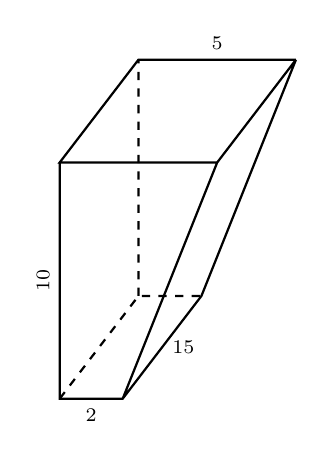
\begin{tikzpicture}[x={(1,0)},z={(0,1)},y={(.5,.87)},xscale=.4,yscale=.3]
\draw [thick] (0,0,0) -- node [above,rotate=90,pos=.5] {\scriptsize 10} (0,0,-10) --  node [below, pos=.5] {\scriptsize 2} (2,0,-10) -- node [right, pos=.5] {\scriptsize 15} (2,5,-10) -- (5,5,0)
							(5,5,0) -- (5,0,0)
							(5,0,0) -- (0,0,0) -- (0,5,0) --  node [above,pos=.5] {\scriptsize 5}(5,5,0)
							(5,0,0) -- (2,0,-10);						

\draw [thick,dashed] (0,0,-10) -- (0,5,-10) -- (2,5,-10)
																	(0,5,-10) -- (0,5,0);
\end{tikzpicture}\hfill\null

\item A conical water tank is 5 m deep with a top radius of 3 m. The tank is filled with pure water, with a mass density of 1000 kg/m$^3$. 
	\begin{enumerate}
	\item		Find the work performed in pumping all the water to the top of the tank.
	\item		Find the work performed in pumping the top 2.5 m of water to the top of the tank.
	\item		Find the work performed in pumping the top half of the water, by volume, to the top of the tank.
	\end{enumerate}

\item A water tank has the shape of a truncated cone, with dimensions given below, and is filled with water with a weight density of 62.4 lb/ft$^3$. Find the work performed in pumping all water to a point 1 ft above the top of the tank.\\

\hfill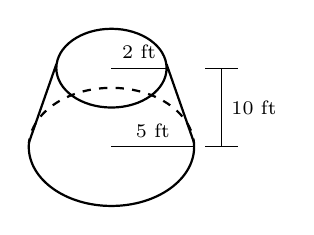
\begin{tikzpicture}[xscale=.7,yscale=.5]\draw [thick] (0,0) circle (1)
							(-1,.1) -- (-1.5,-1.9)
							(1,.1) -- (1.5,-1.9);
\draw (0,0)-- node [above,pos=.5] {\scriptsize 2 ft} (1,0)
			(0,-2) -- node [above,pos=.5] {\scriptsize 5 ft} (1.5,-2)
			(1.7,0) -- (2.3,0)
			(1.7,-2) -- (2.3,-2)
			(2,0) -- node [pos=.5,right] {\scriptsize 10 ft} (2,-2);
\draw [thick] (-1.5,-2) arc (180:360:1.5);
\draw [thick,dashed] (-1.5,-2) arc (180:0:1.5);
\end{tikzpicture}
\hfill\null

\item A water tank has the shape of an inverted pyramid, with dimensions given below, and is filled with water with a mass density of 1000 kg/m$^3$. Find the work performed in pumping all water to a point 5 m above the top of the tank.

\hfill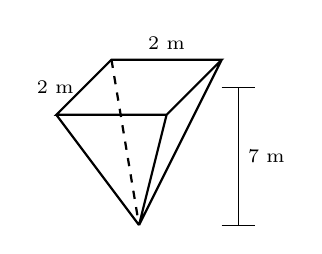
\begin{tikzpicture}[xscale=.7,yscale=.7]
\draw [thick] (0,0) -- node [pos=.5,left]{\scriptsize 2 m} (1,1) --node [above,pos=.5] {\scriptsize 2 m} (3,1) -- (2,0)--cycle
							(0,0) -- (1.5,-2)
							(3,1) -- (1.5,-2)
							(2,0) -- (1.5,-2);
\draw [thick,dashed] (1,1) -- (1.5,-2);
\draw (3,.5) -- (3.6,.5)
			(3,-2) -- (3.6,-2)
			(3.3,.5) -- node [pos=.5,right] {\scriptsize 7 m} (3.3,-2);
\end{tikzpicture}
\hfill\null

\item A water tank has the shape of an truncated, inverted pyramid, with dimensions given below, and is filled with water with a mass density of 1000 kg/m$^3$. Find the work performed in pumping all water to a point 1 m above the top of the tank.

\hfill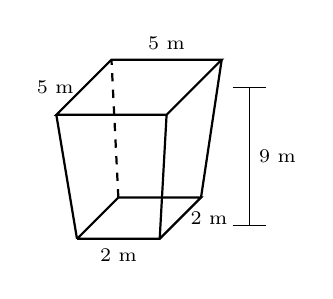
\begin{tikzpicture}[xscale=.7,yscale=.7]
\draw [thick] (0,0) node (A) {}-- node [pos=.5,left]{\scriptsize 5 m} (1,1)node (B) {} --node [above,pos=.5] {\scriptsize 5 m} (3,1) node (C) {} -- (2,0) node (D) {}--cycle;
\begin{scope}[scale=.75,shift={(.5,-3)}]
\draw [thick] (0,0) node (AA) {} -- (1,1) node (BB) {} -- (3,1) node (CC) {} -- node [right,pos=.5] {\scriptsize 2 m} (2,0) node (DD) {}-- node [pos=.5,below]{\scriptsize 2 m} (0,0);
\end{scope}
\draw [dashed,thick] (BB.center) -- (B.center);
\draw [thick] (AA.center) -- (A.center)
							(DD.center) -- (D.center)
							(CC.center) -- (C.center);
\draw (3.2,.5) -- (3.8,.5)
			(3.2,-2) -- (3.8,-2)
			(3.5,.5) -- node [pos=.5,right] {\scriptsize 9 m} (3.5,-2);\end{tikzpicture}
\hfill\null

%\item Consider the curve $f(x) = 3 \cos(\frac{x^3}{4})$ and the portion of its graph that lies in the first quadrant between the $y$-axis and the first positive value of $x$ for which $f(x) = 0$.  Let  $R$ denote the region bounded by this portion of $f$, the $x$-axis, and the $y$-axis.  Assume that $x$ and $y$ are each measured in feet.
%  	\ba
%		\item Picture the coordinate axes rotated 90 degrees clockwise so that the positive $x$-axis points straight down, and the positive $y$-axis points to the right.  Suppose that $R$ is rotated about the $x$ axis to form a solid of revolution, and we consider this solid as a storage tank.  Suppose that the resulting tank is filled to a depth of 1.5 feet with water weighing 62.4 pounds per cubic foot.  Find the amount of work required to lower the water in the tank until it is 0.5 feet deep, by pumping the water to the top of the tank.
%		\item Again picture the coordinate axes rotated 90 degrees clockwise so that the positive $x$-axis points straight down, and the positive $y$-axis points to the right.  Suppose that $R$, together with its reflection across the $x$-axis, forms one end of a storage tank that is 10 feet long.  Suppose that the resulting tank is filled completely with water weighing 62.4 pounds per cubic foot.  Find a formula for a function that tells the amount of work required to lower the water by $h$ feet.
%		\item Suppose that the tank described in (b) is completely filled with water.  Find the total force due to hydrostatic pressure exerted by the water on one end of the tank.
%	\ea 
  
\item A cylindrical tank, buried on its side, has radius 3 feet and length 10 feet.  It is filled completely with water whose weight density is 62.4 lbs/ft$^3$, and the top of the tank is two feet underground.
	\ba
		\item Set up an integral expression that represents the amount of work required to empty the top half of the water in the tank to a truck whose tank lies 4.5 feet above ground.
  
		\item With the tank now only half-full, set up an integral expression that represents the total force due to hydrostatic pressure against one end of the tank.
	\ea

\end{enumerate}

%---------------------------------------------
% END OF EXERCISES ON SECOND PAGE
%---------------------------------------------
\end{multicols*}
\end{adjustwidth*}

\afterexercises 

\cleardoublepage
\section{An Introduction to Differential Equations} \label{S:6.6.DEIntro}

\begin{goals}
\item What is a differential equation and what kinds of information can it tell us?
\item How do differential equations arise in the world around us?
\item What do we mean by a solution to a differential equation?
\item What is a slope field and how can we use a slope field to obtain qualitative information about the solutions of a differential equation?
\item What are stable and unstable equilibrium solutions of an autonomous differential equation? 
\end{goals} 

%---------------------------------------------
% SUBSECTION INTRODUCTION
%---------------------------------------------
\subsection*{Introduction}

In previous chapters, we have seen that a function's derivative tells us the rate at which the function is changing.  More recently, the Fundamental Theorem of Calculus helped us to determine the total change of a function over an interval when we know the function's rate of change.  For instance, an object's velocity tells us the rate of change of that object's position.  By integrating the velocity over a time interval, we may determine by how much the position changes over that time interval.  In particular, if we know where the object is at the beginning of that interval, then we have enough information to accurately predict where it will be at the end of the interval. 

In this section, we will introduce the concept of \emph{differential equations} and explore this idea in more depth.  Simply said, a differential equation is an equation that provides a description of a function's derivative, which means that it tells us the function's rate of change.  Using this information, we would like to learn as much as possible about the function itself.  For instance, we would ideally like to have an algebraic description of the function.  

\begin{pa} \label{PA:7.1}
The position of a moving object is given by the function $s(t)$, where $s$ is measured in feet and $t$ in seconds.  We determine that the velocity is $v(t) = 4t + 1$ feet per second. 
\ba
\item How much does the position change over the time interval   $[0,4]$?

\item Does this give you enough information to determine $s(4)$, the position at time $t=4$?  If so, what is $s(4)$?  If not, what additional information would you need to know to determine $s(4)$?

\item Suppose you are told that the object's initial position $s(0) = 7$.  Determine $s(2)$, the object's position $2$ seconds later. 

\item If you are told instead that the object's initial position is $s(0) = 3$, what is $s(2)$?

\item If we only know the velocity $v(t)=4t+1$, is it possible that the object's position at all times is $s(t) = 2t^2 + t - 4$?  Explain how you know.

\item Are there other possibilities for $s(t)$?  If so, what are they?  

\item If, in addition to knowing the velocity function is $v(t) = 4t+1$, we know the initial position $s(0)$, how many possibilities are there for $s(t)$?
\ea
\end{pa} 
\afterpa
 %PREVIEW 

%-------------------------------------------------------------
% SUBSECTION DIFFERENTIAL EQUATIONS
%-------------------------------------------------------------
\subsection*{What is a differential equation?} \index{differential equation} 

A differential equation is an equation that describes the derivative, or derivatives, of a function that is unknown to us.  For instance, the equation
$$ \frac{dy}{dx} = x \sin(x) $$
is a differential equation since it describes the derivative of a function $y(x)$ that is unknown to us.

As many important examples of differential equations involve quantities that change in time, the independent variable in our discussion will frequently be time $t$. For instance, in the preview activity, we considered the differential equation
$$ \frac{ds}{dt} = 4t + 1. $$
Knowing the velocity and the starting position of the object, we were able to find the position at any later time.

Because differential equations describe the derivative of a function, they give us information about how that function changes.  Our goal will be to take this information and use it to predict the value of the function in the future; in this way, differential equations provide us with something like a crystal ball.

Differential equations arise frequently in our every day world.  For instance, you may hear a bank advertising:

\begin{quote}{\em Your money will grow at a 3\% annual interest rate with us.}\end{quote}

This innocuous statement is really a differential equation.  Let's translate:  $A(t)$ will be amount of money you have in your account at time $t$.  On one hand, the rate at which your money grows is the derivative $dA/dt$.  On the other hand, we are told that this rate is $0.03 A$.  This leads to the differential equation
$$ \frac{dA}{dt} = 0.03 A. $$

This differential equation has a slightly different feel than the previous equation $\frac{ds}{dt} = 4t+1$.  In the earlier example, the rate of change depends only on the independent variable $t$, and we may find $s(t)$ by integrating the velocity $4t+1$.   In the banking example, however, the rate of change depends on the dependent variable $A$, so we'll need some new techniques in order to find $A(t)$.  

\begin{activity} \label{A:6.6.1}  Express the following statements as   differential equations.  In each case, you will need to introduce notation to describe the important quantities in the statement so be sure to clearly state what your notation means.
\ba
	\item The population of a town grows at an annual rate of $1.25$\%. 
        \item A radioactive sample loses $5.6$\% of its mass every day.
        \item You have a bank account that earns $4$\% interest every year.  At the same time, you withdraw money continually from the account at the rate of \$$1000$ per year.
        \item A cup of hot chocolate is sitting in a $70^\circ$ room. The temperature of the hot chocolate cools by $10$\% of the difference between the hot chocolate's temperature and the room temperature every minute.
        \item A can of cold soda is sitting in a $70^\circ$ room. The temperature of the soda warms at the rate of $10$\% of the difference between the soda's temperature and the room's temperature every minute.
\ea
\end{activity}
\begin{smallhint}
\ba
	\item Small hints for each of the prompts above.
\ea
\end{smallhint}
\begin{bighint}
\ba
	\item Big hints for each of the prompts above.
\ea
\end{bighint}
\begin{activitySolution}
\ba
	\item Solutions for each of the prompts above.
\ea
\end{activitySolution}
\aftera %ACTIVITY

Differential equations may be classified based on certain characteristics they may possess.  Indeed, you may see many different types of differential equations in a later course in differential equations.  For now, we would like to introduce a few terms that are used to describe differential equations.

A {\em first-order} differential equation\index{differential equation!first order} is one in which only the first derivative of the function occurs.  For this reason,
$$ \frac{dv}{dt} = 1.5-0.5v $$
is a first-order equation while
$$ \frac{d^2 y}{dt^2} = -10y $$
is a second-order equation.

A differential equation is {\em autonomous}\index{autonomous} \index{differential equation!autonomous} if the independent variable does not  appear in the description of the derivative.  For instance,
$$ \frac{dv}{dt} = 1.5-0.5v $$
is autonomous because the description of the derivative $dv/dt$ does not depend on time.   The equation
$$ \frac{dy}{dt} = 1.5t - 0.5y, $$
however, is not autonomous.

%-------------------------------------------------------------------
% SUBSECTION DE IN THE WORLD AROUND US
%-------------------------------------------------------------------
\subsection*{Differential equations in the world around us}

As we have noted, differential equations give a natural way to describe phenomena we see in the real world.  For instance, physical principles are frequently expressed as a description of how a quantity changes.  A good example is Newton's Second Law, an important physcial principle that says:  

\begin{quote} {\em The product of an object's mass and acceleration equals the force applied to it.} \end{quote}

For instance, when gravity acts on an object near the earth's surface, it exerts a force equal to $mg$, the mass of the object times the gravitational constant $g$.  We therefore have 
\begin{eqnarray*} 
ma & = & mg, \ \mbox{or} \\
\quad \frac{dv}{dt} & = & g,
\end{eqnarray*}
where $v$ is the velocity of the object, and $g = 9.8$ meters per second squared.  Notice that this physical principle does not tell us what the object's velocity is, but rather how the object's velocity changes.  

\begin{activity} \label{A:6.6.2}  
Shown are two graphs depicting the velocity of falling objects.  One is the velocity of a skydiver, while the other is the velocity of a meteorite entering the Earth's atmosphere.

\ba
	\item Begin with the skydiver's velocity and use the given graph to measure the rate of change $dv/dt$ when the velocity is $v=0.5, 1.0, 1.5,
          2.0$, and $2.5$.  Plot your values on the graph below.  You
          will want to think carefully about this:  you are plotting
          the derivative $dv/dt$ as a function of {\em velocity}.

          \begin{center}
            \scalebox{0.65}{\includegraphics{figures/7_1_dataplot.eps}}
          \end{center}
        \item Now do the same thing with the meteorite's velocity:
          use the given graph to measure the rate of change $dv/dt$ when the velocity is
          $v=3.5,4.0,4.5$, and $5.0$.  Plot your values on the graph
          above. 
        \item You should find that all your points lie on a line.
          Write the equation of this line being careful to use proper
          notation for the quantities on the horizontal and vertical
          axes.
        \item The relationship you just found is a differential
          equation.  Write a complete sentence that explains its
          meaning. 
        \item By looking at the differential equation, determine the
          values of the velocity for which the velocity 
          increases.
        \item By looking at the differential equation, determine the
          values of the velocity for which the velocity 
          decreases.
        \item By looking at the differential equation, determine the
          values of the velocity for which the velocity 
          remains constant.

\ea
\end{activity}

\begin{marginfigure}[-6cm]
\begin{center}
\subfloat[Skydiver's velocity]{\includegraphics[scale=.75]{figures/7_1_activity_0.eps}}

\subfloat[Meteorite's velocity]{\includegraphics[scale=.75]{figures/7_1_activity_1.eps}}
\end{center}
\caption{Graphs of velocities used in Activity~\ref{A:6.6.2}.}
\end{marginfigure}


\begin{smallhint}
\ba
	\item Small hints for each of the prompts above.
\ea
\end{smallhint}
\begin{bighint}
\ba
	\item Big hints for each of the prompts above.
\ea
\end{bighint}
\begin{activitySolution}
\ba
	\item Solutions for each of the prompts above.
\ea
\end{activitySolution}
\aftera %ACTIVITY

The point of this activity is to demonstrate how differential equations model processes in the real world.  In this example, two factors are influencing the velocities:  gravity and wind resistance. The differential equation describes how these factors influence the rate of change of the objects' velocities.

%---------------------------------------------
% SUBSECTION SOLVING DE
%---------------------------------------------
\subsection*{Solving a differential equation} \index{differential equation!solution}

We have said that a differential equation is an equation that describes the derivative,  or derivatives, of a function that is unknown to us.  By a {\em   solution} to a differential equation, we mean simply a function that satisfies this description.

For instance, the first differential equation we looked at is 
$$ \frac{ds}{dt} = 4t+1, $$
which describes an unknown function $s(t)$.  We may check that $s(t) = 2t^2+t$ is a solution because it satisfies this description.  Notice that $s(t) = 2t^2+t+4$ is also a solution.

If we have a candidate for a solution, it is straightforward to check whether it is a solution or not.  Before we demonstrate, however, let's consider the same issue in a simpler context. Suppose we are given the equation $2x^2 - 2x = 2x+6$ and asked whether $x=3$ is a solution.  To answer this question, we could rewrite the variable $x$ in the equation with the symbol $\Box$:
$$ 2\Box^2 - 2\Box = 2\Box + 6. $$
To determine whether $x=3$ is a solution, we can investigate the value of each side of the equation separately when the value $3$ is placed in $\Box$ and see if indeed the two resulting values are equal.  Doing so, we observe that 
$$2\Box^2 - 2\Box = 2\cdot3^2 - 2\cdot3 = 12,$$
and
$$2\Box + 6 = 2\cdot3 + 6 = 12.$$
Therefore, $x=3$ is indeed a solution.

We will do the same thing with differential equations.  Consider the differential equation 
\begin{eqnarray*}
\frac{dv}{dt} & = & 1.5 - 0.5v, \ \mbox{or} \\
\quad \frac{d\Box}{dt} & = & 1.5 - 0.5\Box.
\end{eqnarray*}
Let's ask whether $v(t) = 3 - 2e^{-0.5t}$ is a solution\footnote{At this time, don't worry about why we chose this function;  we will learn techniques for finding solutions to differential equations soon enough.  }.  Using this formula for $v$, observe first that
$$\frac{dv}{dt} =  \frac{d\Box}{dt}  = \frac{d}{dt}[3 - 2e^{-0.5t}] = -2e^{-0.5t} \cdot (-0.5) = e^{-0.5t}$$
and
$$1.5 - 0.5v = 1.5 - 0.5\Box= 1.5 - 0.5(3 - 2e^{-0.5t}) = $$
$$1.5 - 1.5 + e^{-0.5t} = e^{-0.5t}.$$
Since $\frac{dv}{dt}$ and $1.5 - 0.5v$ agree for all values of $t$ when $v = 3-2e^{-0.5t}$, we have indeed
found a solution to the differential equation.

\begin{activity} \label{A:7.1.3}  Consider the differential equation 
$$
\frac{dv}{dt} = 1.5 - 0.5v.
$$
Which of the following functions are solutions of this differential equation?
\ba
	\item $v(t) = 1.5t - 0.25t^2$.
        \item $v(t) = 3 + 2e^{-0.5t}$.
        \item $v(t) = 3$.
        \item $v(t) = 3 + Ce^{-0.5t}$ where $C$ is any constant.
\ea
\end{activity}
\begin{smallhint}
\ba
	\item Small hints for each of the prompts above.
\ea
\end{smallhint}
\begin{bighint}
\ba
	\item Big hints for each of the prompts above.
\ea
\end{bighint}
\begin{activitySolution}
\ba
	\item Solutions for each of the prompts above.
\ea
\end{activitySolution}
\aftera %ACTIVITY

This activity shows us something interesting.  Notice that the differential equation has infinitely many solutions, which are parameterized by the constant $C$ in $v(t) = 3+Ce^{-0.5t}$.  In Figure~\ref{F:7.1.family}, we see the graphs of these solutions for a few values of $C$,  as labeled.

\begin{marginfigure}[3cm] % MARGIN FIGURE
\margingraphics{figures/7_1_family.eps}
\caption{The family of solutions to the differential equation $\frac{dv}{dt} = 1.5 - 0.5v$.} \label{F:7.1.family} 
\end{marginfigure}

Notice that the value of $C$ is connected to the initial value of the velocity $v(0)$, since $v(0) = 3+C$.  In other words, while the differential equation describes how the velocity changes as a function of the velocity itself, this is not enough information to determine the velocity uniquely:  we also need to know the initial velocity.  For this reason, differential equations will typically have infinitely many solutions, one corresponding to each initial value.  We have seen this phenomenon before, such as when given the velocity of a moving object $v(t)$, we were not able to uniquely determine the object's position unless we also know its initial position.

If we are given a differential equation and an initial value for the unknown function, we say that we have an {\em initial value problem.} For instance,
$$   \frac{dv}{dt} = 1.5-0.5v, \ v(0) = 0.5 $$
is an initial value problem.  In this situation, we know the value of $v$ at one time and we know how $v$ is changing.  Consequently, there should be exactly one function $v$ that satisfies the initial value problem.

%This demonstrates the following important general property of initial value problems.
%
%\concept{Initial Value Problems}{
%    Initial value problems that are ``well behaved'' have exactly one
%    solution, which exists in some interval around the initial point.
%} % end concept
%
%We won't worry about what ``well behaved'' means---it is a technical
%condition that will be satisfied by all the differential equations we
%consider. 

%---------------------------------------------
% SUBSECTION SLOPE FIELDS
%---------------------------------------------
\subsection{Slope Fields} \index{Slope Fields}

We may sketch the solution to an initial value problem if we know an appropriate collection of tangent lines.  Because we may use a given differential equation to determine the slope of the tangent line at any point of interest, by plotting a useful collection of these, we can get an accurate sense of how certain solution curves must behave.

Let's investigate the differential equation $\ds \frac{dy}{dt} = t-2.$ If $t=0$, this equation says that $dy/dt = 0-2=-2$.  Note that this value holds regardless of the value of $y$.  We will therefore sketch tangent lines for several values of $y$ and $t=0$ with a slope of $-2$; see Figure~\ref{F:6.6_SF1}.  

\begin{marginfigure}[-4cm] %MARGINFIGURE
\begin{center}
\includegraphics{figures/7_2_field_0.eps}
\end{center}
\caption{Beginnings of the slope field for $\ds \frac{dy}{dt} = t-2.$. }
\label{F:6.6_SF1}
\end{marginfigure}

Let's continue in the same way:  if $t=1$, the differential equation tells us that $dy/dt = 1-2=-1$, and this holds regardless of the value of $y$.  We now sketch tangent lines for several values of $y$ and $t=1$ with a slope of $-1$; see Figure~\ref{F:6.6_SF1}-(a).

%\begin{marginfigure} %MARGINFIGURE
%\begin{center}
%\subfloat[]{\includegraphics{figures/7_2_field_1.eps}}
%
%\subfloat[]{\includegraphics{figures/7_2_field_3.eps}}
%
%\subfloat[]{\includegraphics{figures/7_2_field_23a.eps}}
%\end{center}
%\caption{Generating the slope field for $\ds \frac{dy}{dt} = t-2.$.}
%\label{F:6.6_SF2}
%\end{marginfigure}

Similarly, we see that when $t=2$, $dy/dt = 0$ and when $t=3$, $dy/dt=1$.  We may therefore add to our growing collection of tangent line plots; see Figure~\ref{F:6.6_SF1}-(b). In this figure, you may see the solutions to the differential equation emerge.  However, for the sake of clarity, we will add more tangent lines to provide the more complete picture shown in Figure~\ref{F:6.6_SF2}-(c).

\begin{figure*} %MARGINFIGURE
\begin{flushright}
\subfloat[]{\includegraphics{figures/7_2_field_1.eps}}
\hspace{.5cm}
\subfloat[]{\includegraphics{figures/7_2_field_3.eps}}
\hspace{.5cm}
\subfloat[]{\includegraphics{figures/7_2_field_23a.eps}}
\end{flushright}
\caption{Generating the slope field for $\ds \frac{dy}{dt} = t-2.$.}
\label{F:6.6_SF2}
\end{figure*}

Figure~\ref{F:6.6_SF2}-(c) is called a {\em slope field}\index{slope field} for the differential equation, allows us to sketch solutions of the differential equation.  Here, we will begin with the initial value $y(0) = 1$ and start sketching the solution by following the tangent line, as shown in Figure~\ref{F:6.6_SF6}.

%\begin{marginfigure} %MARGINFIGURE
%\margingraphics{figures/7_2_field_30.eps}
%\caption{Sketching a solution curve for $\ds \frac{dy}{dt} = t-2.$. }
%\label{F:6.6_SF5}
%\end{marginfigure}

We then continue using this principle:  whenever the solution passes through a point at which a tangent line is drawn, that line is tangent to the solution.  Doing so leads us to the following sequence of images.

\begin{figure*} % MARGIN FIGURE
\begin{flushright}
\captionsetup[subfigure]{labelformat=empty}
\subfloat{\includegraphics{figures/7_2_field_30.eps}}
\hspace{.25cm}
\subfloat{\includegraphics{figures/7_2_field_31.eps}}
\hspace{.25cm}
\subfloat{\includegraphics{figures/7_2_field_32.eps}}
\hspace{.25cm}
\subfloat{\includegraphics{figures/7_2_field_33.eps}}
\end{flushright}
\caption{Sketching a solution curve for $\ds \frac{dy}{dt} = t-2.$.}
\label{F:6.6_SF6}
\end{figure*}

In fact, we may draw solutions for any possible initial value, and doing this for several different initial values for $y(0)$ results in the graphs shown in Figure~\ref{F:6.6_SF7}.
 
Just as we have done for the most recent example with $\frac{dy}{dt} = t-2$, we can construct a slope field for any differential equation of interest.  The slope field provides us with visual information about how we expect solutions to the differential equation to behave.

\begin{marginfigure} %MARGINFIGURE
\begin{center}
\includegraphics{figures/7_2_field_4.eps}
\end{center}
\caption{Several solution curves for $\ds \frac{dy}{dt} = t-2.$. }
\label{F:6.6_SF7}
\end{marginfigure}

\begin{activity} \label{A:6.6.4}  
  Consider the autonomous differential equation 
$$
\frac{dy}{dt} = -\frac 12( y - 4).
$$

\ba
\item Make a plot of $\frac{dy}{dt}$ versus $y$ on the axes provided.  Looking at the
  graph, for what values of $y$ does $y$ increase and for what values of $y$
  does $y$ decrease?

  \begin{center}
    \includegraphics{figures/7_2_Act1_1.eps}
  \end{center}

\item Next, sketch the slope field for this differential equation on the axes provided.

  \begin{center}
    \includegraphics{figures/7_2_Act1_2.eps}
  \end{center}

\item  Use your work in (b) to sketch the solutions that satisfy $y(0) = 0$, $y(0) = 2$, $y(0) = 4$ 
  and $y(0) = 6.$

\item  Verify that $y(t) = 4 + 2e^{-t/2}$ is a solution to the given
  differential equation with the initial value $y(0) = 6.$  Compare
  its graph to the one you sketched in (c).

\item  What is special about the solution where $y(0) = 4$?  

\ea
\end{activity}
\begin{smallhint}
\ba
	\item Small hints for each of the prompts above.
\ea
\end{smallhint}
\begin{bighint}
\ba
	\item Big hints for each of the prompts above.
\ea
\end{bighint}
\begin{activitySolution}
\ba
	\item Solutions for each of the prompts above.
\ea
\end{activitySolution}
\aftera %ACTIVITY

%-----------------------------------------------------------
% SUBSECTION EQUILIBRIUM SOLUTIONS
%-----------------------------------------------------------
\subsection*{Equilibrium solutions and stability} 

As our work in Activity~\ref{A:6.6.4} demonstrates, first-order autonomous
solutions may have solutions that are constant.  In fact, these are
quite easy to detect by inspecting the differential equation $dy/dt =
f(y)$:  constant solutions necessarily have a zero derivative so 
$dy/dt = 0 = f(y)$.  

For example, in Activity~\ref{A:6.6.4}, we considered the
equation
$$
\frac{dy}{dt} = f(y)=-\frac12(y-4).
$$
Constant solutions are found by setting $f(y) = -\frac12(y-4) = 0$,
which we immediately see implies that $y = 4$.  

Values of $y$ for which $f(y) = 0$ in an autonomous differential equation $\frac{dy}{dt} = f(y)$ are usually called or {\em equilibrium solutions} \index{equilibrium solution} of the differential
equation.  

\begin{marginfigure}[6cm]
\margingraphics{figures/7_2_Act2_1.eps}
\end{marginfigure}

\begin{marginfigure}[1cm]
\margingraphics{figures/7_2_Act2_2.eps}
\end{marginfigure}

\begin{activity} \label{A:7.2.1}  
Consider the autonomous differential equation 
$$ \frac{dy}{dt} = -\frac 12 y(y-4). $$

\ba
\item Make a plot of $\frac{dy}{dt}$ versus $y$.  Looking at the
  graph, for what values of $y$ does $y$ increase and for what values of $y$
  does $y$ decrease?

\item Identify any equilibrium solutions of the given differential equation.

\item Now sketch the slope field for the given differential equation.

\item  Sketch the solutions to the given differential equation that correspond to initial values $y(0)=-1, 0, 1, \ldots, 5$.

\item  An equilibrium solution $\overline{y}$ is called {\em stable} \index{stable} \index{equilibrium solution!stable}
  if nearby 
  solutions converge to $\overline{y}$.  This means that if the inital
  condition varies slightly from $\overline{y}$, then
  $\lim_{t\to\infty}y(t) = \overline{y}$.  

  Conversely, an equilibrium solution $\overline{y}$ 
  is called {\em unstable} \index{unstable} \index{equilibrium solution!unstable} if nearby solutions are pushed away from
  $\overline{y}$.

  Using your work above, classify the equilibrium solutions you found in (b)
  as either stable or unstable.

\item Suppose that $y(t)$ describes the population of a species of
  living organisms and that the initial value $y(0)$ is positive.  What can you
  say about the eventual fate of this population?  

\item  Remember that an equilibrium solution $\overline{y}$ satisfies
  $f(\overline{y}) = 0$.  If we graph $dy/dt = f(y)$ as a function of
  $y$, for which of the following differential equations is
  $\overline{y}$ a stable equilibrium and for which is $\overline{y}$ unstable?  Why?

  \begin{center}
    \includegraphics{figures/7_2_Act2_3.eps} \qquad
    \includegraphics{figures/7_2_Act2_4.eps} 
  \end{center}

\ea
\end{activity}
\begin{smallhint}
\ba
	\item Small hints for each of the prompts above.
\ea
\end{smallhint}
\begin{bighint}
\ba
	\item Big hints for each of the prompts above.
\ea
\end{bighint}
\begin{activitySolution}
\ba
	\item Solutions for each of the prompts above.
\ea
\end{activitySolution}
\aftera %ACTIVITY

%---------------------------------------------
% SUMMARY
%---------------------------------------------
\begin{summary}
\item A differential equation is simply an equation that describes the
  derivative(s) of an unknown function.
\item Physical principles, as well as some everyday situations, often
  describe how a quantity changes, which 
  lead to differential equations.
\item A solution to a differential equation is a function whose
  derivatives satisfy the equation's description.  Differential
  equations typically have infinitely many solutions, 
  parameterized by the initial values.
\item A slope field is a plot created by graphing the tangent lines of
  many different solutions to a differential equation.
\item Once we have a slope field, we may sketch the graph of solutions
  by drawing a curve that is always tangent to the lines in the slope
  field. 
\item Autonomous differential equations sometimes have constant
  solutions that we call 
  equilibrium solutions.  These may be classified as stable or
  unstable, depending on the behavior of nearby solutions.  
\end{summary}

\clearpage

%--------------
% EXERCISES
%--------------
\begin{adjustwidth*}{}{-2.25in}
\textbf{{\large Exercises}}
\setlength{\columnsep}{25pt}
\begin{multicols*}{2}

\noindent {\normalsize Problems} \small

\begin{enumerate}[1)]
 \item Suppose that $T(t)$ represents the temperature of a cup of
    coffee set out in a room, where $T$ is expressed in degrees
    Fahrenheit and $t$ in minutes.  A physical principle known as    Newton's Law of Cooling\index{Newton's Law of Cooling} tells us that 
    $$
    \frac{dT}{dt}= -\frac1{15}T+5.
    $$

\ba
    \item Supposes that $T(0)=105$.  What does the differential
    equation give us for the value of $\ds \frac{dT}{dt}\vert_{T=0}$?  Explain in a
    complete sentence the meaning of these two facts.

    \item Is $T$ increasing or decreasing at $t=0$?

    \item What is the approximate temperature at $t=1$?

    \item On the graph below, make a plot of $dT/dt$ as a function of $T$.
        \begin{center}
          \includegraphics{figures/7_1_exercise_1.eps}
        \end{center}

       \item For which values of $T$ does $T$ increase?  For
        which values of $T$ does $T$ decrease?

        \item What do you think is the temperature of the room?
        Explain your thinking.

        \item Verify that $T(t) = 75 + 30e^{-t/15}$ is the
        solution to the differential equation with initial value $T(0)
        = 105$.  What happens to this solution after a long time?
  \ea
  
  \item Suppose that the population of a particular species is
    described by the function $P(t)$, where $P$ is expressed in
    millions.  Suppose further that the population's rate of change is
    governed by the differential equation 
    $$\frac{dP}{dt} = f(P)
    $$
    where $f(P)$ is the function graphed below.

    \begin{center}
      \includegraphics[scale=.75]{figures/7_1_threshold.eps}
    \end{center}

\ba
    \item For which values of the population $P$ does the population
      increase?

      \item For which values of the population $P$ does the population
      decrease? 

      \item  If $P(0) = 3$, how will the population change in time?

     \item  If the initial population satisfies $0<P(0)<1$, what will
      happen to the population after a very long time?

      \item  If the initial population satisfies $1<P(0)<3$, what will
      happen to the population after a very long time?

      \item If the initial population satisfies $3<P(0)$, what will
      happen to the population after a very long time?

      \item  This model for a population's growth is sometimes called
      ``growth with a threshold.''  Explain why this is an appropriate
      name.  

\ea

  \item In this problem, we test further what it means for a function to be a solution to a given differential equation.
  \ba
  	\item Consider the differential equation
      $$
      \frac{dy}{dt} = y - t.
      $$
      Determine whether the following functions are solutions to the given differential equation.

      \begin{itemize}
 	\item[(i)] $y(t) = t + 1 + 2e^t$
	\item[(ii)] $y(t) = t + 1$
	\item[(iii)] $y(t) = t + 2$
       \end{itemize}

	\item   When you weigh bananas in a scale at the grocery store, the
      height $h$ of the bananas is described by the differential
      equation
      $$
      \frac{d^2h}{dt^2} = -kh
      $$
      where $k$ is the {\em spring constant}, a constant that depends
      on the properties of the spring in the scale.  After you put the
      bananas in the scale, you (cleverly) observe that the height of the bananas
      is given by $h(t) = 4\sin(3t)$.  What is the value of the spring
      constant? 
    \ea
        
\end{enumerate}

%------------------------------------------
% END OF EXERCISES ON FIRST PAGE
%------------------------------------------
\end{multicols*}
\end{adjustwidth*}

\afterexercises 

\cleardoublepage

\section{Separable differential equations} \label{S:6.7.SolvingDE}

\begin{goals}
\item What is a separable differential equation?  
\item How can we find solutions to a separable differential equation?
\item Are some of the differential equations that arise in applications separable?
\item How can we use differential equations to describe and understand 
  phenomena in the world around us?
\end{goals} 

%---------------------------------------------
% SUBSECTION INTRODUCTION
%---------------------------------------------
\subsection*{Introduction}

Given the frequency with which differential equations arise in the world around us, we would like to have some techniques for finding explicit algebraic solutions of certain initial value problems.  In this section, we focus on a particular class of differential equations (called {\em separable}) and develop a method for finding algebraic formulas for solutions to these equations.

A {\em separable differential equation}\index{separable} is a differential equation whose algebraic structure permits the variables present to be separated in a particular way.  For instance, consider the equation
$$ \frac{dy}{dt} = ty. $$
We would like to separate the variables $t$ and $y$ so that all occurrences of $t$ appear on the right-hand side, and all occurrences of $y$ appears on the left and multiply $dy/dt$.  We may do this in the preceding differential equation by dividing both sides by $y$:
$$ \frac1y\frac{dy}{dt} = t. $$
Note particularly that when we attempt to separate the variables in a differential equation, we require that the left-hand side be a product in which the derivative $dy/dt$ is one term.  

Not every differential equation is separable.  For example, if we consider the equation
$$ \frac{dy}{dt} = t-y, $$
it may seem natural to separate it by writing
$$ y + \frac{dy}{dt} = t. $$
As we will see, this will not be helpful since the left-hand side is not a product of a function of $y$ with $\frac{dy}{dt}$.

\begin{pa} \label{PA:7.4}  In this preview activity, we explore whether certain differential equations are separable or not, and then revisit some key ideas from earlier work in integral calculus.
  \ba
\item Which of the following differential equations are separable?  If the equation is separable, write the equation in the revised form $g(y) \frac{dy}{dt} = h(t)$.
  \begin{enumerate}
    \item $\displaystyle \frac{dy}{dt} = -3y$.
    \item $\displaystyle \frac{dy}{dt} = ty - y$.
    \item $\displaystyle \frac{dy}{dt} = t + 1$.
    \item $\displaystyle \frac{dy}{dt} = t^2 - y^2$.
  \end{enumerate}
\item Explain why any autonomous differential equation is guaranteed to be separable.  
\item Why do we include the term ``$+C$'' in the expression $$\int x~dx =
  \frac{x^2}{2} + C?$$  
\item Suppose we know that a certain function $f$ satisfies the equation
  $$
  \int f'(x)~dx = \int x~dx.
  $$
  What can you conclude about $f$?
\ea
\end{pa} 
\afterpa
 %PREVIEW 

%--------------------------------------------------------------------------------
% SUBSECTION SEPERABLE DIFFERENTIAL EQUATIONS
%--------------------------------------------------------------------------------
\subsection*{Solving separable differential equations} \index{separable}

Before we discuss a general approach to solving a separable differential equation, it is instructive to consider an example.

%\begin{marginfigure} % MARGIN FIGURE
%\margingraphics{figures/6_4_DamEx.eps}
%\caption{A trapezoidal dam that is 25 feet tall, 60 feet wide at its base, 90 feet wide at its top, with the water line 5 feet down from the top of its face.} \label{F:6.4.DamEx}
%\end{marginfigure}

\begin{example} \label{eg:6.7.1} % EXAMPLE
Find all functions $y$ that are solutions to the differential equation 
$$\frac{dy}{dt}= \frac{t}{y^2}.$$

\solution We begin by separating the variables and writing
$$ y^2\frac{dy}{dt} = t. $$
Integrating both sides of the equation with respect to the independent variable $t$ shows that
$$ \int y^2\frac{dy}{dt}~dt = \int t~dt. $$
Next, we notice that the left-hand side allows us to change the variable of antidifferentiation from $t$ to $y$.  In particular, $dy = \frac{dy}{dt}~dt$, so we now have
$$ \int y^2 ~dy = \int t~dt. $$
This is why we required that the left-hand side be written as a product in which $dy/dt$ is one of the terms. This most recent equation says that two families of antiderivatives are equal to one another.  Therefore, when we find representative antiderivatives of both sides, we know they must differ by arbitrary constant $C$.  Antidifferentiating and including the integration constant $C$ on the right, we find that
$$ \frac{y^3}{3} = \frac{t^2}{2} + C. $$
    Again, note that it is not necessary to include an arbitrary constant on both sides 
    of the equation;  we know that $y^3/3$ and $t^2/2$ are in the same
    family of antiderivatives and must therefore differ by a single
    constant.

Finally, we may now solve the last equation above for $y$ as a function of $t$, which gives
    $$
    y(t) = \sqrt[3]{\frac 32 \thinspace t^2 + 3C}.
    $$
    Of course, the term $3C$ on the right-hand side represents
    $3$ times an unknown constant.  It is, therefore, still an unknown
    constant, which we will rewrite as $C$.  We thus conclude that the funtion
    $$
    y(t) = \sqrt[3]{\frac 32 \thinspace t^2 + C}
    $$
is a solution to the original differential equation for any value of $C$.

Notice that because this solution depends on the arbitrary constant $C$, we have found an infinite family of
solutions.  This makes sense because we expect to find a unique solution that corresponds to any given
 initial value.

For example, if we want to solve the initial value problem
$$
  \frac{dy}{dt} = \frac{t}{y^2}, \
  y(0) = 2,
$$
we know that the solution has the form $y(t) = \sqrt[3]{\frac32\thinspace
  t^2 + C}$ for some constant $C$.  We therefore must find the appropriate
value for $C$ that gives the initial value $y(0)=2$.  Hence,
$$
  2 = y(0)  \sqrt[3]{\frac 32 \thinspace 0^2 + C} = \sqrt[3]{C},
  $$
which shows that $C = 2^3 = 8$.  The solution to the initial value problem is then
$$
y(t) = \sqrt[3]{\frac32\thinspace t^2+8}.
$$
\end{example}  %EXAMPLE 

The strategy of Example~\ref{eg:6.7.1} may be applied to any differential equation of the form $\frac{dy}{dt} = g(y) \cdot h(t)$, and any differential equation of this form is said to be \emph{separable}.  We work to solve a separable differential equation by writing
$$\frac{1}{g(y)} \frac{dy}{dt} = h(t),$$ 
and then integrating both sides with respect to $t$.  After integrating, we strive to solve algebraically for $y$ in order to write $y$ as a function of $t$.

We consider one more example before doing further exploration in some activities.

%\begin{marginfigure} % MARGIN FIGURE
%\margingraphics{figures/6_4_DamEx.eps}
%\caption{A trapezoidal dam that is 25 feet tall, 60 feet wide at its base, 90 feet wide at its top, with the water line 5 feet down from the top of its face.} \label{F:6.4.DamEx}
%\end{marginfigure}

\begin{example} \label{eg:6.7.2} % EXAMPLE
Solve the differential equation
$$\frac{dy}{dt} =3y.$$

\solution Following the same strategy as in Example~\ref{eg:6.7.1}, we have
$$  \frac 1y \frac{dy}{dt} = 3. $$
Integrating both sides with respect to $t$,
$$  \int \frac 1y\frac{dy}{dt}~dt = \int 3~dt,$$
and thus 
$$ \int \frac 1y~dy =  \int 3~dt.$$
Antidifferentiating and including the integration constant, we find that
$$  \ln|y| = 3t + C.$$
Finally, we need to solve for $y$.  Here, one point deserves careful
attention.  By the definition of the natural logarithm function, it follows that
$$
|y| = e^{3t+C} = e^{3t}e^C.
$$
Since $C$ is an unknown constant, $e^C$ is as well, though we do know
that it is positive (because $e^x$ is positive for any $x$).
When we remove the absolute value in order to solve for $y$, however, this constant may be either positive or
negative.  We 
will denote this updated constant (that accounts for a possible $+$ or $-$) by $C$ to obtain
$$
y(t) = Ce^{3t}.
$$

There is one more slightly technical point to make.  Notice that $y=0$
is an equilibrium solution to this differential equation.  In solving
the equation above, we begin by dividing both sides by $y$, which
is not allowed if $y=0$.  To be perfectly careful, therefore, we will typically
consider the equilibrium solutions separably.  In this case, notice that the final
form of our solution captures the equilibrium solution by allowing
$C=0$. 
\end{example}  %EXAMPLE 

\begin{activity} \label{A:7.4.1}  
Suppose that the population of a town is increases by $3$\% every year.

\ba
\item Let $P(t)$ be the population of the town in year $t$.  Write a
  differential equation that describes the annual growth rate.

\item Find the solutions of this differential equation.

\item If you know that the town's population in year $0$ is $10,000$, find
  the population $P(t)$.

\item How long does it take for the population to double?  This time
  is called the {\em doubling time}.

\item Working more generally, find the doubling time if the annual
  growth rate is $k$ times the population.

\ea
\end{activity}
\begin{smallhint}
\ba
	\item Small hints for each of the prompts above.
\ea
\end{smallhint}
\begin{bighint}
\ba
	\item Big hints for each of the prompts above.
\ea
\end{bighint}
\begin{activitySolution}
\ba
	\item Solutions for each of the prompts above.
\ea
\end{activitySolution}
\aftera  %ACTIVITY   

\begin{activity} \label{A:7.4.2}  
  Suppose that a cup of coffee is initially at a temperature of
  $105$$^\circ$ F and is placed in a $75$$^\circ$ F room.  Newton's law of
  cooling says that 
  $$
  \frac{dT}{dt} = -k(T-75),
  $$ 
  where $k$ is a constant of proportionality.

\ba
\item Suppose you measure that the coffee is cooling at one degree per
  minute at the time the coffee is brought into the room.  Use the
  differential equation to determine the value of the constant $k$.

\item Find all the solutions of this differential equation.

\item What happens to all the solutions as $t\to\infty$?  Explain how
  this agrees with your intuition.

\item What is the temperature of the cup of coffee after $20$ minutes?

\item How long does it take for the coffee to cool to $80^\circ$?

\ea
\end{activity}
\begin{smallhint}
\ba
	\item Small hints for each of the prompts above.
\ea
\end{smallhint}
\begin{bighint}
\ba
	\item Big hints for each of the prompts above.
\ea
\end{bighint}
\begin{activitySolution}
\ba
	\item Solutions for each of the prompts above.
\ea
\end{activitySolution}
\aftera %ACTIVITY

\begin{activity} \label{A:7.4.3}  Solve each of the following differential equations or initial value problems.
\ba
	\item $\ds \frac{dy}{dt} - (2-t) y = 2-t$
	\item $\ds \frac{1}{t}\frac{dy}{dt} = e^{t^2-2y}$
	\item $y' = 2y+2$, \ \ $y(0)=2$
	\item $y' = 2y^2$, \ \ $y(-1) = 2$
	\item $\ds \frac{dy}{dt} = \frac{-2ty}{t^2 + 1}$, \ \  $y(0) = 4$
\ea
\end{activity}
\begin{smallhint}
\ba
	\item Small hints for each of the prompts above.
\ea
\end{smallhint}
\begin{bighint}
\ba
	\item Big hints for each of the prompts above.
\ea
\end{bighint}
\begin{activitySolution}
\ba
	\item Solutions for each of the prompts above.
\ea
\end{activitySolution}
\aftera %ACTIVITY


%--------------------------------------------------------------------------------
% SUBSECTION SEPERABLE DIFFERENTIAL EQUATIONS
%--------------------------------------------------------------------------------
\subsection*{Developing a differential equation}

In our work to date, we have seen several ways that
differential equations arise in the natural world, from the growth of
a population to the temperature of a cup of coffee.  Now,
we will look more closely at how differential equations give us a
natural way to describe various phenoma.  As we'll see, the key is to
focus on understanding the different factors that cause a quantity to
change.

\begin{activity} \label{A:6.7.4}
Any time that the rate of change of a quantity is related to the amount of a quantity, a differential equation naturally arises.  In the following two problems, we see two such scenarios; for each, we want to develop a differential equation whose solution is the quantity of interest.
  \ba
\item Suppose you have a bank account in which money grows at an
  annual rate of $3$\%.
  \begin{itemize}
    \item[(i)] If you have $\$10,000$ in the account, at what rate is your
      money growing?
    \item[(ii)] Suppose that you are also withdrawing money from the account
      at $\$1,000$ per year.  What is the rate of change in the amount
      of money in the account?  What are the units on this rate of change? 
  \end{itemize}
\item Suppose that a water tank holds $100$ gallons and that a salty
  solution, which contains $20$ grams of salt in every gallon, enters the
  tank at $2$ gallons per minute.   
  \begin{itemize}
    \item[(i)] How much salt enters the tank each minute?
    \item[(ii)] Suppose that initially there are $300$ grams of salt in the tank.  How
      much salt is in each gallon at this point in time?
    \item[(iii)] Finally, suppose that evenly mixed solution is pumped out of the tank at the
      rate of $2$ gallons per minute.  How much salt leaves the tank
      each minute?
    \item[(iv)] What is the total rate of change in the amount of salt in
      the tank?
  \end{itemize}
\ea
\end{activity} 
\aftera
 % ACTIVITY

Activity~\ref{A:6.7.4} demonstrates the kind of thinking we will be
doing.  In each of the two examples we considered, there is a
quantity, such as the amount of money in the bank account or the
amount of salt in the tank, that is changing due to several factors.
The governing differential equation results from the total rate of change being the difference between the rate of
increase and the rate of decrease.

\begin{marginfigure}[8cm] % MARGIN FIGURE
\margingraphics{figures/7_5_lake_michigan.eps}
\caption{Plot of $\frac{dP}{dt}$ vs. $P$. } \label{F:6.7.Ex3-1}
\end{marginfigure}

\begin{example} \label{eg:6.7.3} % EXAMPLE
In the Great Lakes region, rivers flowing into the lakes carry a great
deal of pollution in the form of small pieces of plastic averaging $1$
millimeter in diameter.  In order to understand how the amount of
plastic in Lake Michigan is changing, construct a model for how this type pollution has built up in the lake.


\solution First, some basic facts about Lake Michigan.
\begin{itemize}
  \item The volume of the lake is
    $5\cdot10^{12}$ cubic meters.
  \item Water flows into the lake at a rate of
    $5\cdot10^{10}$ cubic meters per year.  It flows out of the lake
    at the same rate.
  \item Each cubic meter flowing
    into the lake contains roughly $3\cdot10^{-8}$ cubic meters of
    plastic pollution.
\end{itemize}

Let's denote the amount of pollution in the lake by $P(t)$, where $P$
is measured in cubic meters of plastic and $t$ in years.  Our goal
is to describe the rate of change of this function;  in other
words, we want to develop a differential equation describing $P(t)$.

First, we will measure how $P(t)$ increases due to pollution flowing
into the lake.  We know that $5\cdot10^{10}$ cubic meters of water
enters the lake every year and each cubic meter of water contains
$3\cdot10^{-8}$ cubic meters of pollution.  Therefore, pollution
enters the lake at the rate of
$$ \left(5\cdot 10^{10} \frac{m^3 \mbox{\ water}}{\mbox{year}}\right) \cdot \left(3\cdot10^{-8} \frac{m^3 \mbox{\ plastic}}{m^3 \mbox{\ water}} \right) = 1.5\cdot 10^3$$
cubic meters of plastic per year.

Second, we will measure how $P(t)$ decreases due to pollution flowing
out of the lake.  If the total amount of pollution is $P$ cubic
meters and the volume of Lake Michigan is $5\cdot 10^{12}$ cubic
meters, then the concentration of plastic pollution in Lake Michigan is
$$
\frac{P}{5\cdot10^{12}} \quad \hbox{cubic meters of plastic per cubic meter of water}.
$$
Since $5\cdot10^{10}$ cubic meters of water flow out each year,and we assume that each cubic meter of water that flows out carries with it the plastic pollution it contains, then
the plastic pollution leaves the lake at the rate of
$$ \left(\frac{P}{5\cdot10^{12}} \frac{m^3 \mbox{\ plastic}}{m^3 \mbox{\ water}} \right) \cdot \left(5\cdot10^{10} \frac{m^3 \mbox{\ water}}{\mbox{year}} \right)=\frac{P}{100} $$
cubic meters of plastic per year.

The total rate of change of $P$ is thus the difference between the rate at which
pollution enters the lake minus the rate at which pollution leaves the
lake;  that is,
\begin{eqnarray*}
\frac{dP}{dt} & = &1.5\cdot10^{3}-\frac{P}{100} \\
                   & = & \frac{1}{100}(1.5\cdot10^{5} - P).
\end{eqnarray*}

We have now found a differential equation that describes the rate
at which the amount of pollution is changing.  To better understand the
behavior of $P(t)$, we now apply some
of the techniques we have recently developed.

Since this is an autonomous differential equation, we can sketch
$dP/dt$ as a function of $P$ and then construct a slope field, as shown in Figure~\ref{F:6.7.Ex3-1} and Figure \ref{F:6.7.Ex3-2}.

These plots both show that $P=1.5\cdot10^5$ is a stable equilibrium.  Therefore,
we should expect that the amount of pollution in Lake Michigan will
stabilize near $1.5\cdot10^5$ cubic meters of pollution.

Next, assuming that there is initially no pollution in the lake, we will
solve the initial value problem
$$
\frac{dP}{dt} = \frac{1}{100}(1.5\cdot10^{5} - P), \ P(0) = 0.
$$
Separating variables, we find that
$$
\frac1{1.5\cdot10^5-P} \frac{dP}{dt} = \frac1{100}.
$$
Integrating with respect to $t$, we have 
$$  \int \frac1{1.5\cdot10^5-P} \frac{dP}{dt}~dt = \int \frac1{100}~dt,$$
and thus changing variables on the left and antidifferentiating on both sides, we find that
\begin{eqnarray*}
  \int \frac{dP}{1.5\cdot10^5-P} &=& \int \frac1{100}~dt \\
  -\ln|1.5\cdot10^5 - P| & = & \frac1{100}t + C
\end{eqnarray*}
Finally, multiplying both sides by $-1$ and using the definition of the logarithm, we find that
\begin{equation} \label{E:7.5.Ex1C}  1.5\cdot10^5 - P = C e^{-t/100}.
\end{equation}
This is a good time to determine the constant $C$.  Since $P =
0$ when $t=0$, we have
$$
1.5\cdot 10^5 - 0 = Ce^0 = C.
$$
In other words, $C=1.5\cdot10^5$. 

Using this value of $C$ in Equation~(\ref{E:7.5.Ex1C}) and solving for $P$, we arrive at the solution
$$ P(t) = 1.5\cdot10^5(1-e^{-t/100}).$$
Superimposing the graph of $P$ on the slope field we saw in Figure \ref{F:6.7.Ex3-1} and Figure \ref{F:6.7.Ex3-2}, we see, as shown in Figure~\ref{F:6.7.Ex3-3}.

We see that, as expected, the amount of plastic pollution stabilizes around
$1.5\cdot10^5$ cubic meters.
\end{example}

\begin{marginfigure}[-16cm] % MARGIN FIGURE
\margingraphics{figures/7_5_slope_field.eps}
\caption{The slope field for the differential equation $\frac{dP}{dt} = \frac{1}{100}(1.5\cdot10^{5} - P)$.} \label{F:6.7.Ex3-2}
\end{marginfigure}

\begin{marginfigure}[-4cm] % MARGIN FIGURE
\margingraphics{figures/7_5_solution.eps}
\caption{The solution $P(t)$ and the slope field for the differential equation $\frac{dP}{dt} = \frac{1}{100}(1.5\cdot10^{5} - P)$.} \label{F:6.7.Ex3-3}
\end{marginfigure}  % EXAMPLE ***Don't forget the figures!!***

There are many important lessons to learn from Example~\ref{eg:6.7.3}.  Foremost is how we can develop a differential equation by thinking about the ``total rate = rate in - rate out'' model.  In addition, we note how we can bring together all of our available understanding (plotting $\frac{dP}{dt}$ vs. $P$, creating a slope field, solving the differential equation) to see how the differential equation describes the behavior of a changing quantity.

Of course, we can also explore what happens when certain aspects of the problem change.  For instance, let's suppose we are at a time when the plastic pollution entering Lake Michigan has
stabilized at $1.5\cdot10^5$ cubic meters, and that new legislation is
passed to prevent this type of pollution entering the lake.  So, there is no longer any inflow of plastic pollution to the lake.  How does the amount of plastic pollution in Lake Michigan now change?  For example, how long does it take for the amount of plastic pollution in the lake to halve?

Restarting the problem at time $t=0$, we now have the modified initial value problem
$$
\frac{dP}{dt} = -\frac{1}{100}P, \ P(0) = 1.5\cdot10^5.
$$
It is a straightforward and familiar exercise to find that the solution to this equation is $P(t) = 1.5\cdot10^5
e^{-t/100}$.  The time that it takes for half of the pollution to flow
out of the lake is given by $T$ where $P(T) = 0.75\cdot10^5$.  Thus, we must solve the equation
$$0.75\cdot10^5 = 1.5\cdot10^5e^{-T/100},$$
or
$$ \frac12 = e^{-T/100}.$$
It follows that 
$$T = -100\thinspace\ln\left(\frac12\right) \approx 69.3 \quad\hbox{years.}$$

In the activities that follow, we explore some other natural settings in which differential equation model changing quantities.

\begin{activity} \label{A:6.7.finance}  
  Suppose you have a bank account that grows by $5$\% every year.

\ba
\item Let $A(t)$ be the amount of money in the account in year $t$.
  What is the rate of change of $A$?

\item Suppose that you are also withdrawing $\$10,000$ per year.  Write
  a differential equation that expresses the total rate of change of
  $A$. 

\item Sketch a slope field for this differential equation, find any
  equilibrium solutions, and identify them as either stable or
  unstable.  Write a sentence or two that describes the significance
  of the stability of the equilibrium solution.

\item Suppose that you initially deposit $\$100,000$ into the account.  How
  long does it take for you to deplete the account?

\item What is the smallest amount of money you would need to have in
  the account to guarantee that you never deplete the money in the
  account? 
\item If your initial deposit is $\$300,000$, how much could you
  withdraw every year without depleting the account?

\ea
\end{activity}
\begin{smallhint}
\ba
	\item Small hints for each of the prompts above.
\ea
\end{smallhint}
\begin{bighint}
\ba
	\item Big hints for each of the prompts above.
\ea
\end{bighint}
\begin{activitySolution}
\ba
	\item Solutions for each of the prompts above.
\ea
\end{activitySolution}
\aftera %ACTIVITY

\begin{activity} \label{A:6.7.iv.drug}  
A dose of morphine is 
        absorbed from the bloodstream of a patient at a rate
        proportional to the amount in the bloodstream.  

        \ba
        \item Write a differential equation for $M(t)$, the amount of
          morphine in the patient's bloodstream, using $k$ as the
          constant proportionality.
        \item 
          Assuming that the initial dose of morphine is $M_0$,
          solve the initial value problem to find $M(t)$.  Use the
          fact that the half-life for the absorption of morphine is
          two hours to find the constant $k$.
        \item Suppose that a patient is given morphine intraveneously
          at the rate of $3$ milligrams per hour.  Write a differential
          equation that combines the intraveneous administration of
          morphine with the body's natural absorption.
        \item Find any equilibrium solutions and determine their
          stability. 
        \item Assuming that there is initially no morphine in the
          patient's bloodstream, solve the initial value problem to
          determine $M(t)$.
        \item What happens to $M(t)$ after a very long time?
        \item Suppose that a doctor asks you to reduce the
          intraveneous rate so that there is eventually $7$ milligrams
          of morphine in the patient's bloodstream.  To what rate
          would you reduce the intraveneous flow?

\ea
\end{activity}
\begin{smallhint}
\ba
	\item Small hints for each of the prompts above.
\ea
\end{smallhint}
\begin{bighint}
\ba
	\item Big hints for each of the prompts above.
\ea
\end{bighint}
\begin{activitySolution}
\ba
	\item Solutions for each of the prompts above.
\ea
\end{activitySolution}
\aftera %ACTIVITY


%--------------------------------------------------------------------------------
% SUBSECTION POPULATION GROWTH
%--------------------------------------------------------------------------------
\subsection*{Population Growth}

We will now begin studying the earth's population.  To get started, some data for the earth's population in recent years that we will use in our investigations is given in Table~\ref{T:earthpop}.

\begin{margintable}[6cm]

\begin{center}
\scalebox{1.25}{
  \begin{tabular}{|c|c|}
    \hline
    Year & Population \\
    \hline
    $1998$ & $5.932$ \\
    $1999$ & $6.008$ \\
    $2000$ & $6.084$ \\
    $2001$ & $6.159$ \\
    $2002$ & $6.234$ \\
    $2005$ & $6.456$ \\
    $2006$ & $6.531$ \\
    $2007$ & $6.606$ \\
    $2008$ & $6.681$ \\
    $2009$ & $6.756$ \\
    $2010$ & $6.831$ \\
    \hline
  \end{tabular}
} % end scalebox
\end{center}

\caption{The earth's recent population (in billions).}
\label{T:earthpop}
\end{margintable}

\begin{activity} \label{A:7.6.1}  
  Our first model will be based on the following assumption:
  \begin{quote}{\em
      The rate of change of the population is proportional to the
      population.  
    }
  \end{quote}

  On the face of it, this seems pretty reasonable.  When there is a
  relatively small number of people, there will be fewer births and
  deaths so the rate of change will be small.  When there is a larger
  number of people, there will be more births and deaths so we expect
  a larger rate of change.

  If $P(t)$ is the population $t$ years after the year $2000$, we may
  express this assumption as
  $$
  \frac{dP}{dt} = kP
  $$
  where $k$ is a constant of proportionality.

\ba
\item Use the data in the table to estimate the derivative $P'(0)$
  using a central difference.  Assume that $t=0$ corresponds to the
  year $2000$.

\item What is the population $P(0)$?

\item Use these two facts to estimate the constant of proportionality
  $k$ in the differential equation.

\item Now that we know the value of $k$, we have the initial
  value problem
  $$
    \frac{dP}{dt} = kP, \ P(0) = 6.084.
  $$
  Find the solution to this initial value problem.

\item What does your solution predict for the population in the year
  $2010$?  Is this close to the actual population given in the table?

\item When does your solution predict that the population will reach
  $12$ billion?

\item What does your solution predict for the population in the year
  $2500$? 

\item Do you think this is a reasonable model for the earth's
  population?  Why or why not?  Explain your thinking using a couple
  of complete sentences. 

\ea
\end{activity}
\begin{smallhint}
\ba
	\item Small hints for each of the prompts above.
\ea
\end{smallhint}
\begin{bighint}
\ba
	\item Big hints for each of the prompts above.
\ea
\end{bighint}
\begin{activitySolution}
\ba
	\item Solutions for each of the prompts above.
\ea
\end{activitySolution}
\aftera %ACTIVITY

Our work in Activity~\ref{A:7.6.1} shows that that the exponential model is fairly accurate for years 
relatively close to $2000$.  However, if we go too far into the
future, the model predicts increasingly large rates of change, which
causes the population to grow arbitrarily large.  This does not make
much sense since it is unrealistic to expect that the earth would be able to support
such a large population.  

The constant $k$ in the differential equation has an important
interpretation.  Let's rewrite the differential equation $\frac{dP}{dt} = kP$ by solving for $k$, so that we have
$$k = \frac{dP/dt}{P}.$$
Viewed in this light, $k$ is the ratio of the rate of change to the
population;  in other words, it is the contribution to the rate of change 
from a single person.  We call this the {\em per capita
  growth rate}\index{per capita growth rate}.

In the exponential model we introduced in Activity~\ref{A:7.6.1}, the per capita growth rate is
constant.  In particular, we are assuming that when the population is
large, the per capita growth rate is the same as when the population
is small.  It is natural to think that the per capita growth rate should
decrease when the population becomes large, since there will not be
enough resources to support so many people.  In other words, we expect that a more realistic model would hold if we assume
that the per capita growth rate depends on the population $P$.

In the previous activity, we computed the per capita growth rate in a
single year by computing $k$, the quotient of $\frac{dP}{dt}$ and $P$ (which we did for $t = 0$).  If we return data and compute the per capita
growth rate over a range of years, we generate the data shown in Figure~\ref{F:6.7.census}-(a), which shows how the per capita growth rate is a function of the population, $P$.  

From the data, we see that the per capita growth rate appears to decrease as
the population increases.  In fact, the points seem to lie very close
to a line, which is shown at two different scales in Figure \ref{F:6.7.census}-(b) and Figure \ref{F:6.7.census}-(c).

\begin{marginfigure}[-6cm] % MARGIN FIGURE
\begin{center}
\subfloat[]{\includegraphics[scale=.75]{figures/7_6_census.eps}}

\subfloat[]{\includegraphics[scale=.75]{figures/7_6_census_1.eps}}

\subfloat[]{\includegraphics[scale=.75]{figures/7_6_census_2.eps}}
\end{center}
\caption{The data and approximations of the per capita growth as a function of population, $P$.}
\label{F:6.7.census}
\end{marginfigure}

Looking at this line carefully, we can find its equation to be
$$
\frac{dP/dt}{P} = 0.025 - 0.002P.
$$
If we multiply both sides by $P$, we arrive at the differential
equation
$$
\frac{dP}{dt} = P(0.025 - 0.002P).
$$
Graphing the dependence of $dP/dt$ on the population $P$, we see that this differential equation demonstrates a quadratic relationship between $\frac{dP}{dt}$ and $P$, as shown in Figure~\ref{F:6.7.logistic}.

The equation $\frac{dP}{dt} = P(0.025 - 0.002P)$ is an example of the {\em logistic equation}, 
and is the second model for population growth that we will consider.  We
have reason to believe that it will be more realistic since the per
capita growth rate is a decreasing function of the population.

Indeed, the graph in Figure~\ref{F:6.7.logistic} shows that there are two equilibrium
solutions, $P=0$, which is unstable, and $P=12.5$, which is a stable
equilibrium.  The graph shows that any solution with $P(0) >0$ will
eventually stabilize around $12.5$.  In other words, our model predicts
the the world's population will eventually stabilize around $12.5$
billion.

\begin{marginfigure}
  \margingraphics{figures/7_6_logistic_de.eps}
  \caption{A plot of $\frac{dP}{dt}$ vs.~$P$ for the differential equation $\frac{dP}{dt} = P(0.025 - 0.002P)$.}
  \label{F:6.7.logistic}
\end{marginfigure}

A prediction for the long-term behavior of the population is a
valuable conclusion to draw from our differential equation.  We would,
however, like to answer some quantitative questions.  For instance,
how long will it take to reach a population of $10$ billion?  To determine this,
we need to find an explicit solution of the equation.  

%--------------------------------------------------------------------------------
% SUBSECTION LOGISTIC DIFFERENTIAL EQUATION
%--------------------------------------------------------------------------------
\subsection*{Solving the logistic differential equation} \index{logistic}

Since we would like to apply the logistic model in more general situations, we state the logistic equation\index{logistic equation} in its more general form,
\begin{equation} \label{E:6.7.logistic}
\frac{dP}{dt} = kP(N-P).
\end{equation}
The equilibrium solutions here are when $P=0$ and $1-\frac PN = 0$,
which shows that $P=N$.  The equilibrium at $P=N$ is called the {\em
  carrying capacity}\index{carrying capacity} of the population for it represents the stable
population that can be sustained by the environment.

We now solve the logistic equation~(\ref{E:6.7.logistic}).  The equation is separable, so we separate the variables
$$
\frac{1}{P(N-P)}\frac{dP}{dt} = k,
$$
and integrate to find that
$$
\int \frac{1}{P(N-P)}~dP = \int k~dt.
$$

To find the antiderivative on the left, we use the partial fraction decomposition
$$
\frac{1}{P(N-P)} = \frac 1N\left[\frac 1P + \frac 1{N-P}\right].
$$
Now we are ready to integrate, with 
$$
\int \frac 1N\left[\frac 1P + \frac 1{N-P}\right] ~dP  =  \int k~dt. 
$$
On the left, observe that $N$ is constant, so we can remove the factor of $\frac{1}{N}$ and antidifferentiate to find that
$$
\frac 1N (\ln|P| - \ln|N-P|)  =  kt + C.
$$
Multiplying both sides of this last equation by $N$ and using an important rule of logarithms, we next find that
$$\ln\left|\frac{P}{N-P}\right| = kNt + C.$$
From the definition of the logarithm, replacing $e^C$ with $C$, and letting $C$ absorb the absolute value signs, we now know that 
$$\frac{P}{N-P} =  Ce^{kNt}.$$
At this point, all that remains is to determine $C$ and solve algebraically for $P$.

If the initial population is $P(0) = P_0$, then it follows that $C = \frac{P_0}{N-P_0}$, so
$$\frac{P}{N-P} = \frac{P_0}{N-P_0}e^{kNt}.$$
We will solve this most recent equation for $P$ by multiplying both sides by
$(N-P)(N-P_0)$ to obtain 
\begin{eqnarray*}
P(N-P_0) &=& P_0(N-P)e^{kNt}  \\
	 &=& P_0Ne^{kNt} - P_0Pe^{kNt}. 
\end{eqnarray*}	 
Swapping the left and right sides, expanding, and factoring, it follows that
\begin{eqnarray*}
P_0Ne^{kNt} & = & P(N-P_0) + P_0 Pe^{kNt}  \\
	& = & P(N-P_0 + P_0e^{kNt}). 
\end{eqnarray*}
Dividing to solve for $P$, we see that
$$P = \frac{P_0Ne^{kNt}}{N-P_0 + P_0e^{kNt}}.$$
Finally, we choose to multiply the numerator and denominator by $\frac{1}{P_0}e^{-kNt}$
to obtain
$$
P(t) = \frac{N}{\left(\frac{N-P_0}{P_0}\right) e^{-kNt} + 1}.
$$

While that was a lot of algebra, notice the result:  we have
found an explicit solution to the initial value problem
$$
  \frac{dP}{dt} = kP(N-P), \ P(0) = P_0,
$$
and that solution\index{logistic equation!solution} is 
\begin{equation}\label{E:7.6.logistic_solution}
P(t) = \frac{N}{\left(\frac{N-P_0}{P_0}\right) e^{-kNt} + 1}.
\end{equation}

For the logistic equation describing the earth's population that we worked with earlier in this section, we have
$$k=0.002, \quad N= 12.5, \quad \hbox{and} \quad P_0 = 6.084.$$
This gives the solution
$$
P(t) = \frac{12.5}{1.0546e^{-0.025t} + 1},
$$
whose graph is shown in Figure~\ref{F:6.7.logistic_sol}
\begin{marginfigure} 
 \margingraphics{figures/7_6_logistic_sol.eps}
\caption{The solution to the logistic equation modeling the earth's population.} \label{F:6.7.logistic_sol}
\end{marginfigure}

Notice that the graph shows the population leveling off at $12.5$ billion, as
we expected, and that the population will be around $10$ billion in the
year $2050$.  These results, which we have found using a relatively simple
mathematical model, agree fairly well with predictions made using a
much more sophisticated model developed by the United Nations.

The logistic equation is useful in other situations, too, as it is good for modeling any situation in which limited growth is possible.  For instance, it could model the spread of a flu virus through a population contained on a cruise ship, the rate at which a rumor spreads within a small town, or the behavior of an animal population on an island.  Again, it is important to realize that through our work in this section, we have completely solved the logistic equation, regardless of the values of the constants $N$, $k$, and $P_0$.  Anytime we encounter a logistic equation, we can apply the formula we found in Equation~(\ref{E:7.6.logistic_solution}).

\begin{activity} \label{A:7.6.2}  
  Consider the logistic equation
  $$ \frac{dP}{dt} = kP(N-P) $$
  with the graph of $\frac{dP}{dt}$ vs.~$P$ shown below.
  \begin{center}
    \includegraphics{figures/7_6_activity_2.eps}
  \end{center}
\ba
\item At what value of $P$ is the rate of change greatest?

\item Consider the model for the earth's population that we created.
  At what value of $P$ is the rate of change greatest?  How does that
  compare to the population in recent years?

\item According to the model we developed, what will the population be
  in the year $2100$?

\item According to the model we developed, when will the population
  reach $9$ billion?

\item Now consider the general solution to the general logistic initial value problem that
  we found, given by
  $$
  P(t) = \frac{N}{\left(\frac{N-P_0}{P_0}\right)e^{-kNt} + 1}.
  $$
  Verify algebraically that $P(0) = P_0$ and that $\lim_{t\to\infty} P(t) = N$.

\ea
\end{activity}
\begin{smallhint}
\ba
	\item Small hints for each of the prompts above.
\ea
\end{smallhint}
\begin{bighint}
\ba
	\item Big hints for each of the prompts above.
\ea
\end{bighint}
\begin{activitySolution}
\ba
	\item Solutions for each of the prompts above.
\ea
\end{activitySolution}
\aftera %ACTIVITY


%---------------------
% SUMMARY
%---------------------
\begin{summary}
\item A separable differential equation is one that may be rewritten
  with all occurrences of the dependent variable multiplying the
  derivative and all occurrences of the independent variable on the
  other side of the equation.
\item We may find the solutions to certain separable differential equations
  by separating variables, integrating with respect to $t$, and ultimately solving the resulting algebraic equation for $y$.
 
\item This technique allows us to solve many important differential
  equations that arise in the world around us.  For instance, questions of
  growth and decay and Newton's Law of Cooling give rise to separable
  differential equations.  

\item If we assume that the rate of growth of a population is
  proportional to the population, we are led to a model in which the
  population grows without bound and at a  rate that grows without bound. 
\item By assuming that the per capita growth rate decreases as the
  population grows, we are led to the logistic model of population
  growth, which predicts that the population will eventually
  stabilize at the carrying capacity.    
\end{summary}

\clearpage

%--------------
% EXERCISES
%--------------
\begin{adjustwidth*}{}{-2.25in}
\textbf{{\large Exercises}}
\setlength{\columnsep}{25pt}
\begin{multicols*}{2}

\noindent {\normalsize Problems} \small

\begin{enumerate}[1)]
\item  The mass of a radioactive sample decays at a rate that is
    proportional to its mass. 
    \ba
  \item Express this fact as a differential equation for the mass
    $M(t)$ using $k$ for the constant of proportionality.
    \item If the initial mass is $M_0$, find an expression for the
      mass $M(t)$.
    \item The {\em half-life} of the sample is the amount of time
      required for half of the mass to decay.  Knowing that the
      half-life of Carbon-14 is 5730 years, find the value of $k$ for
      a sample of Carbon-14.
    \item How long does it take for a sample of Carbon-14 to be
      reduced to one-quarter its original mass?
    \item Carbon-14 naturally occurs in our environment; any
      living organism takes in Carbon-14 when it eats and breathes.  Upon
      dying, however, the organism no longer takes in Carbon-14. 
      
      Suppose that you find remnants of a pre-historic firepit.  By
      analyzing the charred wood in the pit, you determine that the
      amount of Carbon-14 is only 30\% of the amount in living trees.
      Estimate the age of the firepit.  Note this approach is the basic idea behind radiocarbon dating.

      
    \ea

  \item Consider the initial value problem
    
    $$  \frac{dy}{dt} = -\frac ty, \ y(0) = 8$$
    

    \ba
    \item Find the solution of the initial value problem and sketch its
      graph.

    \item For what values of $t$ is the solution defined?  

    \item What is the value of $y$ at the last time that the
      solution is defined? 

    \item By looking at the differential equation, explain why we
      should not expect to find solutions with the value of $y$ you noted in (c).

      \ea

  \item  Suppose that a cylindrical water tank with a hole in the
    bottom is filled with water.  The water, of course, will leak out
    and the height of the water will decrease.  Let $h(t)$ denote the
    height of the water.  A physical principle called {\em Torricelli's
      Law} implies that the height decreases at a rate proportional to
    the square root of the height.

    \ba
    \item Express this fact using $k$ as the constant of
      proportionality.  
    \item Suppose you have two tanks, one with $k=1$ and another with
      $k=10$.  What physical differences would you expect to find?
    \item Suppose you have a tank for which the height decreases at 20
      inches per minute when the water is filled to a depth of 100
      inches.  Find the value of $k$.  
    \item Solve the initial value problem for the tank in part (c), and graph the solution you determine.
    \item How long does it take for the water to run out of the tank?
    \item Is the solution that you found valid for all time $t$?  If
      so, explain how you know this.  If not, explain why not.
    \ea

  \item The {\em Gompertz equation} is a model that is used to
    describe the growth of certain populations.  Suppose that $P(t)$
    is the population of some organism and that
    $$
    \frac{dP}{dt} = -P\ln\left(\frac P3\right) = -P(\ln P - \ln 3).
    $$

    \ba
    \item Sketch a slope field for $P(t)$ over the range $0\leq P\leq
      6$.

    \item Identify any equilibrium solutions and determine whether
      they are stable or unstable.

    \item Find the population $P(t)$ assuming that $P(0) = 1$ and sketch
      its graph.  What happens to $P(t)$ after a very long time?

    \item Find the population $P(t)$ assuming that $P(0) = 6$ and sketch
      its graph.  What happens to $P(t)$ after a very long time?

    \item Verify that the long-term behavior of your solutions agrees
      with what you predicted by looking at the slope field.

      \ea
\end{enumerate}

%------------------------------------------
% END OF EXERCISES ON FIRST PAGE
%------------------------------------------
\end{multicols*}
\end{adjustwidth*}

\afterexercises 

\cleardoublepage
\section{Hyperbolic Functions}\label{sec:hyperbolic}

\begin{goals}
\item What are hyperbolic functions?  
\item What properties do hyperbolic functions possess?
\end{goals} 

%---------------------------------------------
% SUBSECTION INTRODUCTION
%---------------------------------------------
\subsection*{Introduction}

The \textbf{hyperbolic functions} are a set of functions that have many applications to mathematics, physics, and engineering. Among many other applications, they are used to describe the formation of satellite rings around planets, to describe the shape of a rope hanging from two points, and have application to the theory of special relativity. This section defines the hyperbolic functions and describes many of their properties, especially their usefulness to calculus.


%-----------------------------------------------------------
% SUBSECTION HYPERBOLIC FUNCTIONS
%-----------------------------------------------------------
\subsection*{Hyperbolic Functions}

These functions are sometimes referred to as the ``hyperbolic trigonometric functions'' as there are many, many connections between them and the standard trigonometric functions. Figure~\ref{fig:6.8_hyperbolic} demonstrates one such connection. Just as cosine and sine are used to define points on the circle defined by $x^2+y^2=1$, the functions \textbf{hyperbolic cosine} and \textbf{hyperbolic sine} are used to define points on the hyperbola $x^2-y^2=1$.

\begin{marginfigure} % MARGIN FIGURE
\captionsetup[subfigure]{labelformat=empty}
\subfloat{\margingraphics{figures/fighf_circlearea}}

\subfloat{\margingraphics{figures/fighf_hyperbolaarea}}

\caption{Using trigonometric functions to define points on a circle and hyperbolic functions to define points on a hyperbola. The area of the shaded regions are included in them.}
\label{fig:6.8_hyperbolic}
\end{marginfigure}

\definition{Hyperbolic Functions\index{hyperbolic function!definition}}{%DEFINITION
\bmtwo
\begin{enumerate}[1)]
\item	 $\ds \sinh(x) = \frac{e^x-e^{-x}}2$
\item	 $\ds \cosh(x) = \frac{e^x+e^{-x}}2$
\item	 $\ds \tanh (x) = \frac{\sinh (x)}{\cosh (x)}$
\item	 $\ds \csch (x) = \frac{1}{\sinh (x)}$
\item	 $\ds \sech (x) = \frac{1}{\cosh (x)}$
\item	 $\ds \coth (x) = \frac{\cosh (x)}{\sinh (x)}$
\end{enumerate}
\emtwo
} % end definition

These hyperbolic functions are graphed in Figure~\ref{fig:6.8_hyperbolicgraphs}. In the graphs of $\cosh (x)$ and $\sinh (x)$, graphs of $e^x/2$ and $e^{-x}/2$ are included with dashed lines. As $x$ gets ``large,'' $\cosh (x)$ and $\sinh (x)$ each act like $e^x/2$; when $x$ is a large negative number, $\cosh (x)$ acts like $e^{-x}/2$ whereas $\sinh (x)$ acts like $-e^{-x}/2$.

\marginnote{\textbf{Pronunciation Note:} \par ``cosh'' rhymes with ``gosh,'' \par ``sinh'' rhymes with ``pinch,'' and \par ``tanh'' rhymes with ``ranch.''}

Notice the domains of $\tanh (x)$ and $\sech (x)$ are $(-\infty,\infty)$, whereas both $\coth (x)$ and $\csch (x)$ have vertical asymptotes at $x=0$. Also note the ranges of these function, especially $\tanh (x)$: as $x\to\infty$, both $\sinh (x)$ and $\cosh (x)$ approach $e^{-x}/2$, hence $\tanh (x)$ approaches $1$.

\begin{figure} %  FIGURE
\begin{center}
\begin{tabular}{cc}
\includegraphics{figures/fighf_cosh}  & \includegraphics{figures/fighf_sinh} \\[20pt]
\includegraphics{figures/fighf_tanh_coth} &\includegraphics{figures/fighf_sech_csch}
\end{tabular}
\caption{Graphs of the hyperbolic functions.}
\label{fig:6.8_hyperbolicgraphs}
\end{center}
\end{figure}
 
The following example explores some of the properties of these functions that bear remarkable resemblance to the properties of their trigonometric counterparts.


\begin{example} \label{eg:6.8.1} % EXAMPLE
Use the definitions of the hyperbolic functions to rewrite the following expressions.
\bmtwo
\begin{enumerate}[1)]
\item	 $\cosh^2 (x)-\sinh^2(x)$
\item	 $\tanh^2 (x)+\sech^2 (x)$
\item	 $2\cosh (x)\sinh (x)$
\item	 $\frac{d}{dx}\big(\cosh (x)\big)$
\item	 $\frac{d}{dx}\big(\sinh (x)\big)$
\item	 $\frac{d}{dx}\big(\tanh (x)\big)$
\end{enumerate}
\emtwo

\solution
\begin{enumerate}[1)]
\item	 $\begin{aligned}[t]
 \cosh^2(x)-\sinh^2(x) &= \left(\frac{e^x+e^{-x}}2\right)^2 -\left(\frac{e^x-e^{-x}}2\right)^2\\
 						&= \frac{e^{2x}+2e^xe^{-x} + e^{-2x}}4 - \frac{e^{2x}-2e^xe^{-x} + e^{-2x}}4\\
 						&= \frac44=1.
\end{aligned}$\hfill

So $\cosh^2 (x)-\sinh^2(x)=1$.

\item	 $\begin{aligned}[t]
\tanh^2 (x)+\sech^2 (x) &=\frac{\sinh^2(x)}{\cosh^2 (x)} + \frac{1}{\cosh^2 (x)} \\
&= \frac{\sinh^2(x)+1}{\cosh^2 (x)}\qquad \text{\small Now use identity from \#1)}\\
&= \frac{\cosh^2 (x)}{\cosh^2 (x)} = 1
\end{aligned}$\hfill

So $\tanh^2 (x)+\sech^2 (x)=1$.

\item $\begin{aligned}[t]
2\cosh (x)\sinh (x) &= 2\left(\frac{e^x+e^{-x}}2\right)\left(\frac{e^x-e^{-x}}2\right) \\
&= 2 \cdot\frac{e^{2x} - e^{-2x}}4\\
&= \frac{e^{2x} - e^{-2x}}2 = \sinh (2x).\\
\end{aligned}$ \hfill
			
Thus $2\cosh (x)\sinh (x) = \sinh (2x)$.

\item  $\begin{aligned}[t]
\frac{d}{dx}\big(\cosh (x)\big) &= \frac{d}{dx}\left(\frac{e^x+e^{-x}}2\right) \\
&= \frac{e^x-e^{-x}}2\\
&= \sinh (x)
\end{aligned}\hfill$

So $\frac{d}{dx}\big(\cosh (x)\big) = \sinh (x).$
	
\item  $\begin{aligned}[t]
\frac{d}{dx}\big(\sinh (x)\big) &= \frac{d}{dx}\left(\frac{e^x-e^{-x}}2\right) \\
&= \frac{e^x+e^{-x}}2\\
&= \cosh (x)
\end{aligned}\hfill$

So $\frac{d}{dx}\big(\sinh (x)\big) = \cosh (x).$
	
\item  $\begin{aligned}[t]
\frac{d}{dx}\big(\tanh (x)\big) &= \frac{d}{dx}\left(\frac{\sinh (x)}{\cosh (x)}\right) \\
&= \frac{\cosh (x) \cosh (x) - \sinh (x) \sinh (x)}{\cosh^2 (x)}\\
&= \frac{1}{\cosh^2 (x)}\\
&= \sech^2 (x)
\end{aligned}\hfill$

So $\frac{d}{dx}\big(\tanh (x)\big) = \sech^2 (x).$	
\end{enumerate}

\end{example}%EXAMPLE

\begin{activity} \label{A:6.8.1} Compute the following limits.
\bmtwo
\begin{enumerate}[1)]
\item $\ds \lim_{x \rightarrow \infty} \cosh (x)$
\item $\ds \lim_{x \rightarrow \infty} \sinh (x) $
\item $\ds \lim_{x \rightarrow \infty} \tanh (x) $
\item $\ds \lim_{x \rightarrow \infty} (\cosh (x) - \sinh (x)) $
\end{enumerate}
\emtwo
\end{activity}
\begin{smallhint}
\ba
	\item Small hints for each of the prompts above.
\ea
\end{smallhint}
\begin{bighint}
\ba
	\item Big hints for each of the prompts above.
\ea
\end{bighint}
\begin{activitySolution}
\ba
	\item Solutions for each of the prompts above.
\ea
\end{activitySolution}
\aftera % ACTIVITY

The following concept summarizes many of the important identities relating to hyperbolic functions. Each can be verified by referring back to the definition of the hyperbolic functions.

\concept{Useful Hyperbolic Function Properties}{ %CONCEPT
\textbf{Basic Identities}\par
\bmtwo
\begin{enumerate}[1)]\small
\item $\cosh^2(x)-\sinh^2(x)=1$%
\index{hyperbolic function!identities}\index{hyperbolic function!derivatives}\index{hyperbolic function!integrals}\index{derivative!hyperbolic funct.}\index{integration!hyperbolic funct.}%
\item	$\tanh^2(x)+\sech^2(x)=1$
\item	$\coth^2(x)-\csch^2(x) = 1$
\item	$\cosh (2x)=\cosh^2(x)+\sinh^2(x)$
\item	$\sinh (2x) = 2\sinh (x)\cosh (x)$
\item	$\ds\cosh^2(x) = \frac{\cosh (2x)+1}{2}$
\item $\ds \sinh^2(x)=\frac{\cosh (2x)-1}{2}$
\end{enumerate}\normalsize
\emtwo
\textbf{Derivatives}
\bmtwo
\begin{enumerate}[1)]\small
\item $\frac{d}{dx}\big(\cosh (x)\big) = \sinh (x)$
\item $\frac{d}{dx}\big(\sinh (x)\big) = \cosh (x)$
\item $\frac{d}{dx}\big(\tanh (x)\big) = \sech^2 (x)$
\item $\frac{d}{dx}\big(\sech (x)\big) = -\sech (x)\tanh (x)$
\item $\frac{d}{dx}\big(\csch (x)\big) = -\csch (x)\coth (x)$
\item $\frac{d}{dx}\big(\coth (x)\big) = -\csch^2(x)$
\end{enumerate}\normalsize
\emtwo
\textbf{Integrals}
\bmtwo
\begin{enumerate}[1)]\small
\item $\ds\int \cosh (x)\ dx = \sinh (x)+C$
\item $\ds\int \sinh (x)\ dx = \cosh (x)+C$
\item $\ds\int \tanh (x)\ dx = \ln(\cosh (x)) +C$
\item $\ds\int \coth (x)\ dx = \ln|\sinh (x)\,|+C$
\end{enumerate}\normalsize
\emtwo
} %end CONCEPT

\begin{example} \label{eg:6.8.2} % EXAMPLE
Evaluate the following derivatives and integrals.

\begin{enumerate*}[1)]
\item	 $\ds\frac{d}{dx}\big(\cosh (2x)\big)$\hspace{.5cm}
\item	 $\ds\int \sech^2(7t-3)\ dt$\hspace{.5cm}
\item	 $\ds \int_0^{\ln (2)} \cosh (x)\ dx$
\end{enumerate*}

\solution
\begin{enumerate}[1)]
\item Using the Chain Rule directly, we have $\frac{d}{dx} \big(\cosh (2x)\big) = 2\sinh (2x)$.

Just to demonstrate that it works, let's also use the Basic Identity $\cosh (2x) = \cosh^2(x)+\sinh^2(x)$.
\begin{align*}
\frac{d}{dx}\big(\cosh (2x)\big) &= \frac{d}{dx}\big(\cosh^2(x)+\sinh^2(x)\big) \\
&= 2\cosh (x)\sinh (x)+ 2\sinh (x)\cosh (x)\\ 
&= 4\cosh (x)\sinh (x).
\end{align*}
Using another Basic Identity, we can see that $4\cosh (x)\sinh (x) = 2\sinh (2x)$. We get the same answer either way.

\item	  We employ substitution, with $u = 7t-3$ and $du = 7dt$. Then we have:
$$ \int \sech^2 (7t-3)\ dt = \frac17\tanh (7t-3) + C.$$

\item	 $\ds \int_0^{\ln (2)} \cosh (x)\ dx = \sinh (x)\Big|_0^{\ln (2)} = \sinh (\ln (2)) - \sinh (0) = \sinh(\ln (2)).$
\noindent We can simplify this last expression as $\sinh x$ is based on exponentials:
$$\sinh(\ln (2)) = \frac{e^{\ln (2)}-e^{-\ln (2)}}2 = \frac{2-1/2}{2} = \frac34.$$
\end{enumerate}

\end{example}%EXAMPLE

\begin{activity} \label{A:6.8.3} Evaluate the following integrals.
\bmtwo
\begin{enumerate}[1)]
\item $\ds \int \sinh(3x)+x^3 \ dx  $
\item $\ds \int \tanh(x) \ dx ) $
\item $\ds \int \cosh^2(x) \ dx  $
\item $\ds \int \frac{\sinh(x)}{1 +  \cosh^2(x)} \ dx $
\end{enumerate}
\emtwo
\end{activity}
\begin{smallhint}
\ba
	\item Small hints for each of the prompts above.
\ea
\end{smallhint}
\begin{bighint}
\ba
	\item Big hints for each of the prompts above.
\ea
\end{bighint}
\begin{activitySolution}
\ba
	\item Solutions for each of the prompts above.
\ea
\end{activitySolution}
\aftera % ACTIVITY

%-----------------------------------------------------------
% SUBSECTION INVERSE HYPERBOLIC FUNCTIONS
%-----------------------------------------------------------
\subsection*{Inverse Hyperbolic Functions}

Just as the inverse trigonometric functions are useful in certain integrations, the inverse hyperbolic functions are useful with others. Table~\ref{T:hfinverse2} shows the restrictions on the domains to make each function one-to-one and the resulting domains and ranges of their inverse functions. Their graphs are shown in Figure~\ref{fig:hfinverse1}.\index{hyperbolic function!inverse}

\begin{margintable}[0cm] % MARGIN TABLE
\begin{tabular}{ccc}
Function & Domain & Range\\ \hline
$\cosh (x)$ & $[0,\infty)$ & $[1,\infty)$\\
$\sinh (x)$ & $(-\infty,\infty)$ & $(-\infty,\infty)$\\
$\tanh (x)$ & $(-\infty,\infty)$ & $(-1,1)$\\
$\sech (x)$ & $[0,\infty)$ & $(0,1]$ \\
$\csch (x)$ & $(-\infty,0) \cup (0,\infty)$ & $(-\infty,0) \cup (0,\infty)$\\
$\coth (x)$ & $(-\infty,0) \cup (0,\infty)$ & $(-\infty,-1) \cup (1,\infty)$
\end{tabular}
\caption{Domains and ranges of the hyperbolic functions.} \label{T:6.8_hyper1}
\end{margintable}

\begin{margintable}[0cm] % MARGIN TABLE
\begin{tabular}{ccc}
Function & Domain & Range\\ \hline
\rule{0pt}{10pt}$\cosh^{-1} (x)$ & $[1,\infty)$ & $[0,\infty)$ \\
$\sinh^{-1} (x)$ & $[-\infty,\infty)$ & $[-\infty,\infty)$\\
$\tanh^{-1} (x)$ & $(-1,1)$ & $(-\infty,\infty)$\\
$\sech^{-1} (x)$ & $(0,1]$ & $[0,\infty)$ \\
$\csch^{-1} (x)$ & $(-\infty,0) \cup (0,\infty)$ & $(-\infty,0) \cup (0,\infty)$\\
$\coth^{-1} (x)$ & $(-\infty,-1) \cup (1,\infty)$ & $(-\infty,0) \cup (0,\infty)$
\end{tabular}
\caption{Domains and ranges of the inverse hyperbolic functions.}\label{T:hfinverse2}
\end{margintable}

Because the hyperbolic functions are defined in terms of exponential functions, their inverses can be expressed in terms of logarithms. It is often more convenient to refer to $\sinh^{-1} x$ than to $\ln\big(x+\sqrt{x^2+1}\big)$, especially when one is working on theory and does not need to compute actual values. On the other hand, when computations are needed, technology is often helpful but many hand-held calculators lack a \textit{convenient} $\sinh^{-1}x$ button. (Often it can be accessed under a menu system, but not conveniently.) In such a situation, the logarithmic representation is useful.

In next concept, both the inverse hyperbolic and logarithmic function representations of the antiderivative are given. Again, these latter functions are often more useful than the former. Note how inverse hyperbolic functions can be used to solve integrals we used Trigonometric Substitution to solve in Section~\ref{S:5.3.TrigSub}.

\begin{figure} % FIGURE
\begin{minipage}{1.3\textwidth}
\begin{tabular}{ccc}
\includegraphics[scale=0.95]{figures/fighfarccosh} & \ \hskip 15pt\ &\includegraphics[scale=0.95]{figures/fighfarcsinh}\\[15pt]
\includegraphics[scale=0.95]{figures/fighfarctanharccoth} & &\includegraphics[scale=0.95]{figures/fighfarcsecharccsch}
\end{tabular}
\captionsetup{type=figure}%
\caption{Graphs of the hyperbolic functions and their inverses.}\label{fig:hfinverse1}
\end{minipage}
\end{figure}

\concept{Logarithmic definitions of Inverse Hyperbolic Functions}{ % CONCEPT 
\begin{enumerate}[1)]
\item $\ds\cosh^{-1}(x)=\ln\big(x+\sqrt{x^2-1}\big);\ x\geq1$\index{hyperbolic function!inverse!logarithmic def.}\rule[-10pt]{0pt}{20pt}
\item $\ds\tanh^{-1}(x) = \frac12\ln\left(\frac{1+x}{1-x}\right);\ |x|<1$\rule[-10pt]{0pt}{20pt}
\item $\ds \sech^{-1}(x) = \ln\left(\frac{1+\sqrt{1-x^2}}x\right);\ 0<x\leq1$\rule[-10pt]{0pt}{20pt}
\item $\ds\sinh^{-1}(x) = \ln\big(x+\sqrt{x^2+1}\big)$\rule[-10pt]{0pt}{20pt}
\item	 $\ds\coth^{-1}(x) = \frac12\ln\left(\frac{x+1}{x-1}\right);\ |x|>1$\rule[-10pt]{0pt}{20pt}
\item $\ds\csch^{-1}(x) = \ln\left(\frac1x+\frac{\sqrt{1+x^2}}{|x|}\right);\ x\neq0$\rule[-10pt]{0pt}{20pt}
\end{enumerate}
} % END CONCEPT

The following concepts give the derivatives and integrals relating to the inverse hyperbolic functions. 

\concept{Derivatives Involving Inverse Hyperbolic Functions \index{derivative!inverse hyper.}\index{hyperbolic function!inverse!derivative}}{% CONCEPT
\begin{enumerate}[1)]
\item $\ds\frac{d}{dx}\big(\cosh^{-1} (x)\big) = \frac{1}{\sqrt{x^2-1}};\ x>1$
\item $\ds\frac{d}{dx}\big(\sinh^{-1} (x)\big) = \frac{1}{\sqrt{x^2+1}}$
\item $\ds\frac{d}{dx}\big(\tanh^{-1} (x)\big) = \frac{1}{1-x^2};\ |x|<1$
\item $\ds\frac{d}{dx}\big(\sech^{-1} (x)\big) = \frac{-1}{x\sqrt{1-x^2}}; 0<x<1$
\item $\ds\frac{d}{dx}\big(\csch^{-1} (x)\big) = \frac{-1}{|x|\sqrt{1+x^2}};\ x\neq0$
\item $\ds\frac{d}{dx}\big(\coth^{-1} (x)\big) = \frac{1}{1-x^2};\ |x|>1$
\end{enumerate}
}% end concept

\begin{activity} \label{A:6.8.2} Differentiate the following functions.
\begin{enumerate}[1)]
\item $\ds \frac{d}{dx}( \sinh(3x+x^3) )  $
\item $\ds \frac{d}{dx}( \arccos( \tanh(x) ) ) $
\item $\ds \frac{d}{dx}( \sinh^{-1} (3 \tanh (3x)) ) $
\item $\ds \frac{d}{dx}( \cosh^{-1}(\sqrt{x^2+1})  ) $
\item Show that $f(t) = \cosh(\sqrt{3}t) - \frac{2}{\sqrt{3}}\sinh(\sqrt{3}t)$ is a solution to the differential equation $f''-3f=0$.  
\end{enumerate}
\end{activity}
\begin{smallhint}
\ba
	\item Small hints for each of the prompts above.
\ea
\end{smallhint}
\begin{bighint}
\ba
	\item Big hints for each of the prompts above.
\ea
\end{bighint}
\begin{activitySolution}
\ba
	\item Solutions for each of the prompts above.
\ea
\end{activitySolution}
\aftera % ACTIVITY

\concept{Integrals Involving Inverse Hyperbolic Functions \index{integration!inverse hyper.}\index{hyperbolic function!inverse!integration}}{% CONCEPT
\begin{enumerate}[1)]
\item \begin{align*}
\ds\int \frac{1}{\sqrt{x^2-a^2}}\ dx &= \cosh^{-1}\left(\frac xa\right)+C;\ 0<a<x\\
&= \ds\ln\Big|x+\sqrt{x^2-a^2}\Big|+C
\end{align*}

\item \begin{align*}
\ds\int \frac{1}{\sqrt{x^2+a^2}}\ dx &= \sinh^{-1}\left(\frac xa\right)+C;\ a>0 \\
&= \ds\ln\Big|x+\sqrt{x^2+a^2}\Big|+C
\end{align*}

\item \begin{align*}
\ds\int \frac{1}{a^2-x^2}\ dx &= \left\{\begin{array}{ccc} \frac1a\tanh^{-1}\left(\frac xa\right)+C & & x^2<a^2 \\ \\
\frac1a\coth^{-1}\left(\frac xa\right)+C & & a^2<x^2 \end{array}\right.\\
&= \ds\frac12\ln\left|\frac{a+x}{a-x}\right|+C
\end{align*}

\item \begin{align*}
\ds\int \frac{1}{x\sqrt{a^2-x^2}}\ dx &= -\frac1a\sech^{-1}\left(\frac xa\right)+C;\ 0<x<a \\
&= \ds \frac1a \ln\left(\frac{x}{a+\sqrt{a^2-x^2}}\right)+C 
\end{align*}

\item	 \begin{align*}
\ds\int \frac{1}{x\sqrt{x^2+a^2}}\ dx &= -\frac1a\csch^{-1}\left|\frac xa\right| + C;\ x\neq 0,\ a>0 \\
&= \ds \frac1a \ln\left|\frac{x}{a+\sqrt{a^2+x^2}}\right|+C 
\end{align*}
\end{enumerate}
}% end CONCEPT

\begin{example} \label{eg:6.8.3} % EXAMPLE
Evaluate the following.

\begin{enumerate*}[1)]
\item	$\ds \frac{d}{dx}\left[\cosh^{-1}\left(\frac{3x-2}{5}\right)\right]$ \hspace{.25cm}
\item	$\ds \int\frac{1}{x^2-1}\ dx$ \hspace{.25cm}
\item	$\ds \int \frac{1}{\sqrt{9x^2+10}}\ dx$
\end{enumerate*}

\solution
\begin{enumerate}[1)]
\item	 Applying the concepts along with the Chain Rule gives:
$$\frac{d}{dx}\left[\cosh^{-1}\left(\frac{3x-2}5\right)\right] = \frac{1}{\sqrt{\left(\frac{3x-2}5\right)-1}}\cdot\frac35.$$

\item Multiplying the numerator and denominator by $(-1)$ gives: $\ds \int \frac{1}{x^2-1}\ dx = \int \frac{-1}{1-x^2}\ dx$. The second integral can be solved with a direct application of item \#3 from the integral concepts, with $a=1$. Thus
\begin{align*}
\int \frac{1}{x^2-1}\ dx &= -\int \frac{1}{1-x^2}\ dx  \\
&= \left\{\begin{array}{ccc} -\tanh^{-1}\left(x\right)+C & & x^2<1 \\ \\ -\coth^{-1}\left(x\right)+C & & 1<x^2 \end{array}\right. \\
&=-\frac12\ln\left|\frac{x+1}{x-1}\right|+C\\
&=\frac12\ln\left|\frac{x-1}{x+1}\right|+C.
\end{align*}

%The key to linking the two seemingly different answers together is Figure \ref{fig:hfinverse5}, where the logarithmic definitions of the inverse hyperbolic functions are given. Note that the definitions of $\tanh^{-1}x$ and $\coth^{-1}x$ are very similar; the conditions placed on $|x|$ ensure that the argument of $\ln$ is always positive. Thus one could say 
%$$\frac12\ln\left|\frac{x+1}{x-1}\right| = \left\{\begin{array}{ccc} \tanh^{-1}x+C & & |x|<1 \\ \\
%\coth^{-1}x+C & & |x|>1 \end{array}\right..$$
%
%We reconcile the two answers by returning to Equation \ref{eq:hf3} and continuing:
%\begin{align*}
%\int \frac{1}{x^2-1}\ dx &= \int \frac{-1}{1-x^2}\ dx \\
%			&= \left\{\begin{array}{ccc} -\frac1a\tanh^{-1}\left(\frac xa\right)+C & & x^2<a^2 \\ \\
%-\frac1a\coth^{-1}\left(\frac xa\right)+C & & a^2<x^2 \end{array}\right. \\
%			&= -\frac12\ln\left|\frac{x+1}{x-1}\right|+C \\
%			&= -\frac12\ln|x+1| + \frac12\ln|x-1| +C,
%\end{align*}
%matching the answer previously obtained.

\item	 This requires a substitution; let $u = 3x$, hence $du = 3dx$. We have 
\begin{align*}
\int \frac{1}{\sqrt{9x^2+10}}\ dx &= \frac13\int\frac{1}{\sqrt{u^2+10}}\ du. \\
\intertext{Note $a^2=10$, hence $a = \sqrt{10}.$ Now apply the integral rule.}
 &= \frac13 \sinh^{-1}\left(\frac{3x}{\sqrt{10}}\right) + C \\
 &= \frac13 \ln \Big|3x+\sqrt{9x^2+10}\Big|+C.
\end{align*}
\end{enumerate}

\end{example}%EXAMPLE

%-----------------------------------------------------------
% SUMMARY
%-----------------------------------------------------------
\begin{summary}
\item The hyperbolic functions are similar to trigonometric functions in that they both can represent distances from the origin to a conic section.
\end{summary}

\clearpage

%--------------
% EXERCISES
%--------------
\begin{adjustwidth*}{}{-2.25in}
\textbf{{\large Exercises}}
\setlength{\columnsep}{25pt}
\begin{multicols*}{2}

\noindent {\normalsize Problems} \small

\noindent{\bf In Exercises 1--8, verify the identity.}

\begin{enumerate}[1)]
\item $\coth^2 x-\csch^2x=1$

\item $\cosh 2x = \cosh^2x+\sinh^2x$

\item $\ds\cosh^2x = \frac{\cosh2x+1}{2}$

\item $\ds\sinh^2x = \frac{\cosh2x-1}{2}$

\item $\ds\frac{d}{dx}\left[\sech x\right] = -\sech x\tanh x$

\item $\ds\frac{d}{dx}\left[\coth x\right] = -\csch^2x$

\item $\ds \int \tanh x\ dx  = \ln (\cosh x) + C$

\item $\ds \int \coth x\ dx  = \ln |\sinh x| + C$
\end{enumerate}

\noindent{\bf In Exercises 9--19, differentiate the given function.}

\begin{enumerate}[1),resume]

\item $f(x) = \cosh 2x$

\item $f(x) = \tanh (x^2)$

\item $f(x) = \ln(\sinh x)$

\item $f(x) = \sinh x\cosh x$

\item $f(x) = x\sinh x-\cosh x$

\item $f(x) = \sech^{-1} (x^2)$

\item $f(x) = \tanh^{-1} (\cos x)$

\item $f(x) = \cosh^{-1} (\sec x)$

\item $f(x) = \sinh^{-1} (3x)$

\item $f(x) = \cosh^{-1} (2x^2)$

\item $f(x) = \tanh^{-1} (x+5)$
\end{enumerate}

\noindent{\bf In Exercises 20--24, produce the equation of the line tangent to the function at the given $x$-value.}

\begin{enumerate}[1),resume]
\item $f(x) = \sinh x$ at $x=0$
\item $f(x) = \cosh x$ at $x=\ln 2$
\item $f(x) = \sech^2 x$ at $x=\ln 3$
\item $f(x) = \sinh^{-1} x$ at $x=0$
\item $f(x) = \cosh^{-1} x$ at $x=\sqrt 2$
\end{enumerate}

\noindent{\bf In Exercises 25--36, evaluate the given indefinite integral.}

\begin{enumerate}[1),resume]
\item $\ds \int \tanh (2x)\ dx$
\item $\ds \int \cosh (3x-7)\ dx$
\item $\ds \int \sinh x\cosh x\ dx$
\item $\ds \int \frac{1}{9-x^2}\ dx$
\item $\ds \int \frac{2x}{\sqrt{x^4-4}}\ dx$
\item $\ds \int \frac{\sqrt{x}}{\sqrt{1+x^3}}\ dx$
\item $\ds \int \frac{1}{x^4-16}\ dx$
\item $\ds \int \frac{1}{x^2+x}\ dx$
\item $\ds \int \frac{e^x}{e^{2x}+1}\ dx$
\item $\ds \int \sinh^{-1}x \ dx$
\item $\ds \int \tanh^{-1}x \ dx$
\item $\ds \int \sech x \ dx$ \quad(Hint: mutiply by $\frac{\cosh x}{\cosh x}$; set $u = \sinh x$.)

\end{enumerate}

\noindent{\bf In Exercises 37--39, evaluate the given definite integral.}

\begin{enumerate}[1),resume]
\item $\ds \int_{-1}^1 \sinh x \ dx$
\item $\ds \int_{-\ln 2}^{\ln 2} \cosh x \ dx$
\item $\ds \int_{0}^{1} \tanh^{-1} x \ dx$
\end{enumerate}

%------------------------------------------
% END OF EXERCISES ON FIRST PAGE
%------------------------------------------
\end{multicols*}
\end{adjustwidth*}

\afterexercises 

\cleardoublepage
%\chapter{Sequences \& Series}\label{CH:7}

\section{Sequences} \label{S:7.1.Sequences}

\begin{goals}
\item What is a sequence?
\item What does it mean for a sequence to converge?
\item What does it mean for a sequence to diverge?
\end{goals}

%-----------------------------------
% SUBSECTION INTRODUCTION
%-----------------------------------
\subsection*{Introduction}

We encounter sequences every day. Your monthly rent payments, the annual interest you earn on investments, a list of your car's miles per gallon every time you fill up; all are examples of sequences. Other sequences with which you may be familiar include the Fibonacci sequence\index{Fibonacci sequence}
\[1, 1, 2, 3, 5, 8, \ldots\]
in which each entry is the sum of the two preceding entries and the triangular numbers\index{triangular numbers}
\[1, 3, 6, 10, 15, 21, 28, 36, 45, 55, \ldots\]
which are numbers that correspond to the number of vertices seen in the triangles in Figure \ref{F:8.1.Triangular_numbers}.
\begin{marginfigure}[-4cm] % MARGIN FIGURE
\margingraphics{figures/8_1_Triangular_Numbers.eps}
\caption{Triangular numbers}
\label{F:8.1.Triangular_numbers}
\end{marginfigure}
Sequences of integers are of such interest to mathematicians and others that they have a journal\footnote{\emph{The Journal of Integer Sequences} at \url{http://www.cs.uwaterloo.ca/journals/JIS/}} devoted to them and an on-line encyclopedia\footnote{The On-Line Encyclopedia of Integer Sequences at \url{http://oeis.org/}} that catalogs a huge number of integer sequences and their connections. Sequences are also used in digital recordings and digital images. 

To this point, most of our studies in calculus have dealt with continuous information (e.g., continuous functions). The major difference we will see now is that sequences model \emph{discrete} instead of continuous information. We will study ways to represent and work with discrete information in this chapter as we investigate \emph{sequences} and \emph{series}, and ultimately see key connections between the discrete and continuous.

\begin{margintable}[8cm]
\begin{center}
%\renewcommand{\arraystretch}{1.5}
\begin{tabular}{|c|c|c|} \hline
Month   &Interest earned    &Total amount \\ \hline
$0$       &$\$0$              &$\$5000.00$  \\ \hline
$1$       &$\$33.33$          &$\$5033.33$  \\ \hline
$2$       &                   &\\ \hline
$3$       &                   &\\ \hline
$4$       &                   &\\ \hline
$5$       &                   &\\ \hline
$6$       &                   &\\ \hline
$7$       &                   &\\ \hline
$8$       &                   &\\ \hline
$9$       &                   &\\ \hline
$10$      &                   &\\ \hline
$11$      &                   &\\ \hline
$12$      &                   &\\ \hline
\end{tabular}
\caption{Interest}
\label{T:PA_8.1.Interest}
\end{center}
\end{margintable}

\begin{pa} \label{PA:8.1}
Suppose you receive $\$5000$ through an inheritance. You decide to invest this money into a fund that pays $8\%$ annually, compounded monthly. That means that each month your investment earns $\frac{0.08}{12} \cdot P$ additional dollars, where $P$ is your principal balance at the start of the month. So in the first month your investment earns
\[5000 \left(\frac{0.08}{12}\right)\]
or $\$33.33$. If you reinvest this money, you will then have $\$5033.33$ in your account at the end of the first month. From this point on, assume that you reinvest all of the interest you earn.
    \ba
    \item How much interest will you earn in the second month? How much money will you have in your account at the end of the second month?

    \item Complete Table \ref{T:PA_8.1.Interest} to determine the interest earned and total amount of money in this investment each month for one year.

    \item As we will see later, the amount of money $P_n$ in the account after month $n$ is given by
    \[P_n = 5000\left(1+\frac{0.08}{12}\right)^{n}.\]
    Use this formula to check your calculations in Table \ref{T:PA_8.1.Interest}. Then find the amount of money in the account after $5$ years.
    
    \item How many years will it be before the account has doubled in value to $\$10000$?

\ea
\end{pa}
\afterpa  % PREVIEW ACTIVITY

%-------------------------------
% SUBSECTION SEQUENCES
%-------------------------------
\subsection*{Sequences} \index{sequence}

As our discussion in the introduction and Preview Activity \ref{PA:8.1} illustrate, many discrete phenomena can be represented as lists of numbers (like the amount of money in an account over a period of months). We commonly refer to a set of events that occur one after the other as a \textit{sequence} of events. In mathematics, we use the word \textit{sequence} to refer to an ordered set of numbers, i.e., a set of numbers that ``occur one after the other.''

For instance, the numbers 2, 4, 6, 8, \ldots, form a sequence. The order is important; the first number is 2, the second is 4, etc. It seems natural to seek a formula that describes a given sequence, and often this can be done. For instance, the sequence above could be described by the function $a(n) = 2n$, for the values of $n = 1, 2, \ldots$ To find the 10$^\text{th}$ term in the sequence, we would compute $a(10)$. This leads us to the following, formal definition of a sequence.

\definition{Sequence}{
A \textbf{sequence} is a function $a(n)$ whose domain is $\mathbb{N}$. The \textbf{range} of a sequence is the set of all distinct values of $a(n)$.
\index{sequences!definition}\\

The \textbf{terms} of a sequence are the values $a(1)$, $a(2)$, \ldots, which are usually denoted with subscripts as $a_1$, $a_2$, \ldots.\\

A sequence $a(n)$ is often denoted as $\{a_n\}$.
}% end definition

If the terms are all 0 after some fixed value of $n$, we say the sequence is finite. Otherwise the sequence is infinite. We will work with both finite and infinite sequences, but focus more on the infinite sequences. With infinite sequences, we are often interested in their end behavior and the idea of \emph{convergent} sequences.

\begin{activity} \label{7.1.Act1}
\ba
\item Let $s_n$ be the $n$th term in the sequence $1, 2, 3, \ldots$. 

Find a formula for $s_n$ and use appropriate technological tools to draw a graph of entries in this sequence by plotting points of the form $(n,s_n)$ for some values of $n$. Most graphing calculators can plot sequences; directions follow for the TI-84.
\begin{itemize}
\item In the MODE menu, highlight SEQ in the FUNC line and press ENTER.
\item In the Y= menu, you will now see lines to enter sequences. Enter a value for $n$Min (where the sequence starts), a function for $u(n)$ (the $n$th term in the sequence), and the value of $u_{n\text{Min}}$.
\item Set your window coordinates (this involves choosing limits for $n$ as well as the window coordinates XMin, XMax, YMin, and YMax.
\item The GRAPH key will draw a plot of your  sequence.
\end{itemize}
Using your knowledge of limits of continuous functions as $x \to \infty$, decide if this sequence $\{s_n\}$ has a limit as $n \to \infty$. Explain your reasoning.

\item Let $s_n$ be the $n$th term in the sequence $1, \frac{1}{2}, \frac{1}{3}, \ldots$. Find a formula for $s_n$. Draw a graph of some points in this sequence. Using your knowledge of limits of continuous functions as $x \to \infty$, decide if this sequence $\{s_n\}$ has a limit as $n \to \infty$. Explain your reasoning.

\item Let $s_n$ be the $n$th term in the sequence $2, \frac{3}{2}, \frac{4}{3}, \frac{5}{4}, \ldots$. Find a formula for $s_n$. Using your knowledge of limits of continuous functions as $x \to \infty$, decide if this sequence $\{s_n\}$ has a limit as $n \to \infty$. Explain your reasoning.

\ea
\end{activity}

\begin{smallhint}
\ba
	\item Small hints for each of the prompts above.
\ea
\end{smallhint}
\begin{bighint}
\ba
	\item Big hints for each of the prompts above.
\ea
\end{bighint}
\begin{activitySolution}
\ba
	\item By observation we see that a formula for $s_n$ is $s_n = n$. A plot of the first 50 points in the sequence is shown here.
%\begin{center} 
%\resizebox{!}{1.75in}{\includegraphics{figures/8_1_Sequence_n.eps}} 
%\end{center}
We recalling that a function $f$ has a limit $L$ at infinity if we can make the values of $f(x)$ as large as we want by choosing $x$ as large as we need. Since we can make the values of $n$ in our sequence as large as we want by choosing $n$ to be as large as we need, we suspect that this sequence does not have a limit as $n$ goes to infinity.

\item By observation we see that a formula for $s_n$ is $s_n = \frac{1}{n}$. A plot of the first 50 points in the sequence is shown here.
%\begin{center} \resizebox{!}{1.75in}{\includegraphics{figures/8_1_Sequence_1overn.eps}} \end{center}
Since we can make the values of $\frac{1}{n}$ in our sequence as close to 0 as we want by choosing $n$ to be as large as we need, we suspect that this sequence has a limit of 0 as $n$ goes to infinity.

\item Since the numerator is always 1 more than the denominator, a formula for $s_n$ is $s_n = \frac{n+1}{n}$. A plot of the first 50 points in the sequence is shown here.
%\begin{center} \resizebox{!}{1.75in}{\includegraphics{figures/8_1_Sequence_nplus1overn.eps}} \end{center}
Since we can make the values of $\frac{n+1}{n}$ in our sequence as close to 1 as we want by choosing $n$ to be as large as we need, we suspect that this sequence has a limit of 1 as $n$ goes to infinity.

\ea
\end{activitySolution}
\aftera  % ACTIVITY

Next we formalize the ideas from Activity~\ref{7.1.Act1}.

\begin{activity} \label{7.1.Act2}
\ba
\item State clearly what it means for a continuous function $f$ to have a limit $L$ as $x \to \infty$.

\item Given that an infinite sequence of real numbers is a function from the integers to the real numbers, apply the idea from part (a) to explain what you think it means for a sequence $\{s_n\}$ to have a limit as $n \to \infty$.  

\item Based on your response to (b), decide if the sequence $\left\{ \frac{1+n}{2+n}\right\}$ has a limit as $n \to \infty$. If so, what is the limit? If not, why not?

\ea
\end{activity}

\begin{smallhint}
\ba
	\item Small hints for each of the prompts above.
\ea
\end{smallhint}
\begin{bighint}
\ba
	\item Big hints for each of the prompts above.
\ea
\end{bighint}
\begin{activitySolution}
\ba
	\item A continuous function $f$ has a limit $L$ as the independent variable $x$ goes to infinity if we can make the values of $f(x)$ as close to $L$ as we want by choosing $x$ as large as we need. 
    \item We expect that a sequence $\{s_n\}$ will have a limit $L$ as $n$ goes to infinity if we can make the entries $s_n$ in the sequence as close to $L$ as we want by choosing $n$ as large as we need.
    \item As $n$ gets large, the constant terms become infinitesimally small compared to $n$ and so $\frac{1+n}{2+n}$ looks like $\frac{n}{n}$ or 1 for large $n$. So the sequence $\left\{ \frac{1+n}{2+n}\right\}$ has a limit of 1 at infinity.   
\ea
\end{activitySolution}
\aftera  % ACTIVITY

\begin{marginfigure}[4cm] % MARGIN FIGURE
\subfloat[]{\margingraphics{figures/figseq1a}}

\subfloat[]{\margingraphics{figures/figseq1b}}

\subfloat[]{\margingraphics{figures/figseq1c}}
\caption{Plotting sequences from Example~\ref{eg:7.1.1}.} \label{F:eg:7.1.1}
\end{marginfigure}

\begin{example} \label{eg:7.1.1} % EXAMPLE
List the first four terms of the following sequences.

\begin{enumerate}[1), leftmargin=*]
\item $\ds \{a_n\} = \left\{\frac{3^n}{n!}\right\}$
\item $\{a_n\} = \{4+(-1)^n\}$
\item $\ds \{a_n\} = \left\{\frac{(-1)^{n(n+1)/2}}{n^2}\right\}$
\end{enumerate}

\solution
\begin{enumerate}[1)]
\item	 $\ds a_1=\frac{3^1}{1!} = 3$; $\ds a_2= \frac{3^2}{2!} = \frac92$; $\ds a_3 = \frac{3^3}{3!} = \frac92$; $\ds a_4 = \frac{3^4}{4!} = \frac{27}8$

We can plot the terms of a sequence with a scatter plot. The ``$x$''-axis is used for the values of $n$, and the values of the terms are plotted on the $y$-axis. To visualize this sequence, see Figure~\ref{F:eg:7.1.1}-(a).\\

\item		$a_1= 4+(-1)^1 = 3$;\qquad $a_2 = 4+(-1)^2 = 5$; 

\noindent $a_3=4+(-1)^3 = 3$; \qquad $a_4 = 4+(-1)^4 = 5$. Note that the range of this sequence is finite, consisting of only the values 3 and 5. This sequence is plotted in Figure \ref{F:eg:7.1.1}-(b).\\

\item		$\ds a_1= \frac{(-1)^{1(2)/2}}{1^2} = -1$; \qquad $\ds a_2 = \frac{(-1)^{2(3)/2}}{2^2} =-\frac14$

\noindent $\ds a_3 = \frac{(-1)^{3(4)/2}}{3^2} = \frac19$ \qquad $\ds a_4 = \frac{(-1)^{4(5)/2}}{4^2} = \frac1{16}$; 

\noindent $\ds a_5 = \frac{(-1)^{5(6)/2}}{5^2}=-\frac1{25}$.

\noindent We gave one extra term to begin to show the pattern of signs is ``$-$, $-$, $+$, $+$, $-$, $-$, $\ldots$, due to the fact that the exponent of $-1$ is a special quadratic. This sequence is plotted in Figure \ref{F:eg:7.1.1}-(c).
\end{enumerate}
\end{example}

\begin{example} \label{eg:7.1.2} % EXAMPLE
Find the $n^\text{th}$ term of the following sequences, i.e., find a function that describes each of the given sequences.

\begin{enumerate}[1)]
\item $2, 5, 8, 11, 14, \ldots$
\item $2, -5, 10, -17, 26, -37, \ldots$
\item $1, 1, 2, 6, 24, 120, 720, \ldots$
\item $\ds \frac52, \frac52, \frac{15}8, \frac54, \frac{25}{32}, \ldots$
\end{enumerate}

\solution We should first note that there is never exactly one function that describes a finite set of numbers as a sequence. There are many sequences that start with $2$, then $5$, as our first example does. We are looking for a simple formula that describes the terms given, knowing there is possibly more than one answer.
\begin{enumerate}[1)]
\item		Note how each term is $3$ more than the previous one. This implies a linear function would be appropriate: $a(n) = a_n = 3n + b$ for some appropriate value of $b$. As we want $a_1=2$, we set $b=-1$. Thus $a_n = 3n-1$.

\item		First notice how the sign changes from term to term. This is most commonly accomplished by multiplying the terms by either $(-1)^n$ or $(-1)^{n+1}$. Using $(-1)^n$ multiplies the odd terms by $(-1)$; using $(-1)^{n+1}$ multiplies the even terms by $(-1)$. As this sequence has negative even terms, we will multiply by $(-1)^{n+1}$. 

After this, we might feel a bit stuck as to how to proceed. At this point, we are just looking for a pattern of some sort: what do the numbers $2$, $5$, $10$, $17$, etc., have in common? There are many correct answers, but the one that we'll use here is that each is one more than a perfect square. That is, $2=1^1+1$, $5=2^2+1$, $10=3^2+1$, etc. Thus our formula is $a_n= (-1)^{n+1}(n^2+1)$.

\item		One who is familiar with the factorial function will readily recognize these numbers. They are $0!$, $1!$, $2!$, $3!$, etc. Since our sequences start with $n=1$, we cannot write $a_n = n!$, for this misses the $0!$ term. Instead, we shift by $1$, and write $a_n = (n-1)!$.

\item		This one may appear difficult, especially as the first two terms are the same, but a little ``sleuthing'' will help. Notice how the terms in the numerator are always multiples of $5$, and the terms in the denominator are always powers of $2$. Does something as simple as $a_n = \frac{5n}{2^n}$ work?

When $n=1$, we see that we indeed get $5/2$ as desired. When $n=2$, we get $10/4 = 5/2$. Further checking shows that this formula indeed matches the other terms of the sequence.
\end{enumerate}
\end{example}

A common mathematical endeavor is to create a new mathematical object (for instance, a sequence) and then apply previously known mathematics to the new object. We do so here. The fundamental concept of calculus is the limit, so we will investigate what it means to find the limit of a sequence.

\definition{Limit of a Sequence, Convergent, Divergent} %DEFINITION
{Let $\{a_n\}$ be a sequence and let $L$ be a real number. Given any $\epsilon>0$, if an $m$ can be found such that $|a_n-L|<\epsilon$ for all $n>m$, then we say the \textbf{limit of $\{a_n\}$, as $n$ approaches infinity, is $L$}, denoted $$\lim_{n\to\infty}a_n = L.$$

If $\ds\lim_{n\to\infty} a_n$ exists, we say the sequence \emph{converges}; otherwise, the sequence \emph{diverges}.\index{limit!of sequence}\index{sequences!limit}\index{convergence!of sequence}\index{divergence!of sequence}\index{sequences!convergent}\index{sequences!divergent}
} %end DEFINITION

This definition states, informally, that if the limit of a sequence is $L$, then if you go far enough out along the sequence, all subsequent terms will be \emph{really close} to $L$. Of course, the terms ``far enough'' and ``really close'' are subjective terms, but hopefully the intent is clear.

This definition is reminiscent of the $\epsilon$--$\delta$ proofs of Chapter~\ref{CH:1}. In that chapter we developed other tools to evaluate limits apart from the formal definition; we do so here as well.

\concept{Limit of a Sequence}  %concept
{Let $\{a_n\}$ be a sequence and let $f(x)$ be a function where $f(n) = a_n$ for all $n$ in $\mathbb{N}$. 
\begin{enumerate}
\item		If $\ds \lim_{x\to\infty} f(x) = L$, then $\ds\lim_{n\to\infty} a_n = L$.
\item		If $\ds \lim_{x\to\infty} f(x)$ does not exist, then $\{a_n\}$ diverges.
\end{enumerate}
} %end concept

When we considered limits before, the domain of the function was an interval of real numbers. Now, as we consider limits, the domain is restricted to $\mathbb{N}$, the natural numbers; this restriction of the domain does not affect the outcome of the limit and whatever tools we developed in Chapter~\ref{CH:1} to evaluate limits can be applied here as well.

\begin{example} \label{eg:7.1.3} % EXAMPLE
Determine the convergence or divergence of the following sequences.

\begin{enumerate}[1)]
\item $\ds\{a_n\} = \left\{\frac{3n^2-2n+1}{n^2-1000}\right\}$
\item $\{a_n\} = \{\cos n \}$
\item  $\ds\{a_n\} = \left\{\frac{(-1)^n}{n}\right\}$
\end{enumerate}

\solution
\begin{enumerate}[1)]
\item We can state that $\ds\lim_{x\to\infty} \frac{3x^2-2x+1}{x^2-1000} = 3$. (We could have also directly applied l'H\^opital's Rule.) Thus the sequence $\{a_n\}$ converges, and its limit is $3$. A scatter plot of every $5$ values of $a_n$ is given in Figure \ref{fig:eg:7.1.3}-(a). The values of $a_n$ vary widely near $n=30$, ranging from about $-73$ to $125$, but as $n$ grows, the values approach $3$.

\item The limit $\ds\lim_{x\to\infty}\cos x$ does not exist, as the function oscillates (and takes on every value in $[-1,1]$ infinitely many times). Thus we conclude that the sequence $\{\cos n\}$ diverges. (And in this particular case, since the domain is restricted to $\mathbb{N}$, no value of $\cos n$ is repeated!) This sequence is plotted in Figure \ref{fig:eg:7.1.3}-(b); because only discrete values of cosine are plotted, it does not bear strong resemblance to the familiar cosine wave.

\item The function $f(x) = (-1)^x/x$ is not well defined. (What does $(-1)^{\sqrt{2}}$ mean? In actuality, there is an answer, but it involves \emph{complex analysis}, beyond the scope of this text.) So for now we say that we cannot determine the limit. (But we will be able to very soon.) By looking at the plot in Figure \ref{fig:eg:7.1.3}-(c), we would like to conclude that the sequence converges to $0$. That is true, but at this point we are unable to decisively say so.
\end{enumerate}
\end{example}

\begin{marginfigure}[-4CM] % MARGIN FIGURE
\subfloat[]{\margingraphics{figures/figseq4a}}

\subfloat[]{\margingraphics{figures/figseq4b}}

\subfloat[]{\margingraphics{figures/figseq4c}}
\caption{Scatter plots of the sequences in Example \ref{eg:7.1.3}.}\label{fig:eg:7.1.3}
\end{marginfigure}

\begin{activity} \label{7.1.Act3} Use graphical and/or algebraic methods to determine whether each of the following sequences converges or diverges.
\ba
\item $\ds \left\{\frac{1+2n}{3n-2}\right\}$


\item $\ds \left\{\frac{5+3^n}{10+2^n}\right\}$

\item $\ds \left\{\frac{10^n}{n!}\right\}$ (where $!$ is the \emph{factorial} symbol and $n! = n(n-1)(n-2) \cdots (2)(1)$ for any positive integer $n$ (as convention we define $0!$ to be 1)).

\ea
\end{activity}

\begin{smallhint}
\ba
	\item Small hints for each of the prompts above.
\ea
\end{smallhint}
\begin{bighint}
\ba
	\item Big hints for each of the prompts above.
\ea
\end{bighint}
\begin{activitySolution}
\ba
	\item A plot of the first 50 terms of the sequence $\left\{\frac{1+2n}{3n-2}\right\}$ is shown here.
\begin{center} \resizebox{!}{1.75in}{\includegraphics{figures/8_2_Sequence_a.eps}} \end{center}
The plot implies that the sequence has a limit between 0.5 and 1. For large $n$ the $2n$ term dominates the numerator and the $3n$ term the denominator. So $\frac{1+2n}{3n-2}$ looks like $\frac{2n}{3n} = \frac{2}{3}$ when $n$ is big. So the sequence $\left\{\frac{1+2n}{3n-2}\right\}$ converges to $\frac{2}{3}$.
    \item A plot of the first 50 terms of the sequence $\left\{\frac{5+3^n}{10+2^n}\right\}$ is shown here.
\begin{center} \resizebox{!}{1.75in}{\includegraphics{figures/8_2_Sequence_b.eps}} \end{center}
The plot implies that the sequence does not have a limit as $n$ goes to infinity. For large $n$ the $3^n$ term dominates the numerator and the $2^n$ term the denominator. So $\frac{5+3^n}{10+2^n}$ looks like $\frac{3^n}{2^n} = \left(\frac{3}{2}\right)^n$ when $n$ is big. Since $\frac{3}{2} > 1$, the sequence $\left\{\frac{5+3^n}{10+2^n}\right\}$ diverges to infinity.
    \item A plot of the first 50 terms of the sequence $\left\{\frac{10^n}{n!}\right\}$ is shown here.
\begin{center} \resizebox{!}{1.75in}{\includegraphics{figures/8_2_Sequence_b.eps}} \end{center}
Initially, it looks as though the terms increase without bound, but beginning at about $n=10$ the factorial in the denominator dominates the numerator. Notice that
 \[\frac{10^n}{n!} = \frac{10 \times 10 \times 10 \times \cdots \times 10}{1 \times 2 \times 3 \times \cdots n}\]
When $n > 20$, we have that $\frac{10}{n} < \frac{1}{2}$ and 
\begin{align*}
\frac{10^n}{n!} &= \left(\frac{10 \times 10 \times 10 \times \cdots \times 10}{1 \times 2 \times 3 \times \cdots 20}\right) \left(\frac{10 \times 10 \times 10 \times \cdots \times 10}{21 \times 22 \times 23 \times \cdots n}\right) \\
    &= \left(\frac{10^{20}}{20!}\right) \left(\frac{10}{21}\right) \left(\frac{10}{22}\right) \cdots \left(\frac{10}{n}\right)  \\
    &< \left(\frac{10^{20}}{20!}\right) \left(\frac{1}{2}\right)^{n-20}.
\end{align*}
Since $\frac{1}{2}<1$, the term $\left(\frac{1}{2}\right)^{n-20}$ goes to 0 as $n$ goes to infinity. The fact that $\frac{10^{20}}{20!}$ is a constant means that $\frac{10^n}{n!} \to 0$ as $n \to \infty$. 

\ea
\end{activitySolution}
\aftera  % ACTIVITY

It seems very clear that a sequence such as $\ds \left\{\frac{(-1)^n}{n}\right\}$ converges to 0 but we lack the formal tool to prove it. The following theorem gives us that tool.

\concept{Absolute Value Theorem} %concept
{Let $\{a_n\}$ be a sequence. If $\ds \lim_{n\to\infty} |a_n| = 0$, then $\ds \lim_{n\to\infty} a_n = 0$\index{Absolute Value Theorem}\index{limit!Absolute Value Theorem}\index{sequence!Absolute Value Theorem}
} % end concept

\begin{example} \label{eg:7.1.4} % EXAMPLE
Let the following sequences, and their limits, be given:

\begin{itemize}
\item $\ds \{a_n\} = \left\{\frac{n+1}{n^2}\right\}$, and $\ds \lim_{n\to\infty} a_n = 0$;
\item $\ds \{b_n\} = \left\{\left(1+\frac1n\right)^{n}\right\}$, and $\ds \lim_{n\to\infty} b_n = e$; and
\item $\ds \{c_n\} = \big\{n\cdot \sin (5/n)\big\}$, and $\ds \lim_{n\to\infty} c_n = 5$.
\end{itemize}

Evaluate the following limits.

\begin{enumerate}[1)]
\item $\ds \lim_{n\to\infty} (a_n+b_n)$ 
\item $\ds \lim_{n\to\infty} (b_n\cdot c_n)$ 
\item $\ds \lim_{n\to\infty} (1000\cdot a_n)$
\end{enumerate}

\solution
\begin{enumerate}[1)] 
\item Since $\ds \lim_{n\to\infty} a_n = 0$ and $\ds \lim_{n\to\infty} b_n = e$, we conclude that $\ds \lim_{n\to\infty} (a_n+b_n) = 0+e = e.$ So even though we are adding something to each term of the sequence $b_n$, we are adding something so small that the final limit is the same as before.

\item Since $\ds \lim_{n\to\infty} b_n = e$ and $\ds \lim_{n\to\infty} c_n = 5$, we conclude that $\ds \lim_{n\to\infty} (b_n\cdot c_n) = e\cdot 5 = 5e.$

\item Since $\ds \lim_{n\to\infty} a_n = 0$, we have $\ds \lim_{n\to\infty} 1000a_n =1000\cdot 0 = 0$. It does not matter that we multiply each term by $1000$; the sequence still approaches $0$. (It just takes longer to get close to $0$.)
\end{enumerate}
\end{example}

%-------------------------------
% SUBSECTION SEQUENCES PROPERTIES
%-------------------------------
\subsection*{Properties of Sequences} %\index{sequence}

We continue our study of the limits of sequences by considering some of the properties of these limits.

\concept{Properties of the Limits of Sequences} %concept
{Let $\{a_n\}$ and $\{b_n\}$ be sequences such that $\ds \lim_{n\to\infty} a_n = L$, $\ds \lim_{n\to\infty} b_n = K$, and let $c$ be a real number.

\begin{minipage}[t]{.5\linewidth}
\begin{enumerate}
\item		$\ds \lim_{n\to\infty} (a_n\pm b_n) = L\pm K$
\index{sequences!limit properties}
\item		$\ds \lim_{n\to\infty} (a_n\cdot b_n) = L\cdot K$
\end{enumerate}
\end{minipage}
\begin{minipage}[t]{.5\linewidth}
\begin{enumerate}\addtocounter{enumi}{2}
\item		$\ds \lim_{n\to\infty} (a_n/b_n) = L/K$, $K\neq 0$
\item		$\ds \lim_{n\to\infty} c\cdot a_n = c\cdot L$
\end{enumerate}
\end{minipage}
} %end concept


\begin{example} \label{eg:7.1.5} % EXAMPLE
Determine the boundedness of the following sequences.

\begin{enumerate}[1)]
\item $\ds\{a_n\}  = \left\{\frac1n\right\}$ 
\item $\{a_n\} = \{2^n\}$
\end{enumerate}

\solution
\begin{enumerate}[1)]
\item The terms of this sequence are always positive but are decreasing, so we have $0<a_n<2$ for all $n$. Thus this sequence is bounded. Figure \ref{fig:eg:7.1.5}-(a) illustrates this.

\item The terms of this sequence obviously grow without bound. However, it is also true that these terms are all positive, meaning $0<a_n$. Thus we can say the sequence is unbounded, but also bounded below. Figure \ref{fig:eg:7.1.5}-(b) illustrates this.
\end{enumerate}
\end{example}

\begin{marginfigure}
\subfloat[]{\margingraphics{figures/figseq3a}}

\subfloat[]{\margingraphics{figures/figseq3b}}
\caption{A plot of $\{a_n\} = \{1/n\}$ and $\{a_n\} = \{2^n\}$ from Example \ref{eg:7.1.5}.}
\label{fig:eg:7.1.5}
\end{marginfigure}

\begin{activity} \label{7.1.Act3} Use graphical and/or algebraic methods to determine whether each of the following sequences converges or diverges.
\ba
\item $\ds \left\{\frac{1+2n}{3n-2}\right\}$


\item $\ds \left\{\frac{5+3^n}{10+2^n}\right\}$

\item $\ds \left\{\frac{10^n}{n!}\right\}$ (where $!$ is the \emph{factorial} symbol and $n! = n(n-1)(n-2) \cdots (2)(1)$ for any positive integer $n$ (as convention we define $0!$ to be 1)).

\ea
\end{activity}

\begin{smallhint}
\ba
	\item Small hints for each of the prompts above.
\ea
\end{smallhint}
\begin{bighint}
\ba
	\item Big hints for each of the prompts above.
\ea
\end{bighint}
\begin{activitySolution}
\ba
	\item A plot of the first 50 terms of the sequence $\left\{\frac{1+2n}{3n-2}\right\}$ is shown here.
\begin{center} \resizebox{!}{1.75in}{\includegraphics{figures/8_2_Sequence_a.eps}} \end{center}
The plot implies that the sequence has a limit between 0.5 and 1. For large $n$ the $2n$ term dominates the numerator and the $3n$ term the denominator. So $\frac{1+2n}{3n-2}$ looks like $\frac{2n}{3n} = \frac{2}{3}$ when $n$ is big. So the sequence $\left\{\frac{1+2n}{3n-2}\right\}$ converges to $\frac{2}{3}$.
    \item A plot of the first 50 terms of the sequence $\left\{\frac{5+3^n}{10+2^n}\right\}$ is shown here.
\begin{center} \resizebox{!}{1.75in}{\includegraphics{figures/8_2_Sequence_b.eps}} \end{center}
The plot implies that the sequence does not have a limit as $n$ goes to infinity. For large $n$ the $3^n$ term dominates the numerator and the $2^n$ term the denominator. So $\frac{5+3^n}{10+2^n}$ looks like $\frac{3^n}{2^n} = \left(\frac{3}{2}\right)^n$ when $n$ is big. Since $\frac{3}{2} > 1$, the sequence $\left\{\frac{5+3^n}{10+2^n}\right\}$ diverges to infinity.
    \item A plot of the first 50 terms of the sequence $\left\{\frac{10^n}{n!}\right\}$ is shown here.
\begin{center} \resizebox{!}{1.75in}{\includegraphics{figures/8_2_Sequence_b.eps}} \end{center}
Initially, it looks as though the terms increase without bound, but beginning at about $n=10$ the factorial in the denominator dominates the numerator. Notice that
 \[\frac{10^n}{n!} = \frac{10 \times 10 \times 10 \times \cdots \times 10}{1 \times 2 \times 3 \times \cdots n}\]
When $n > 20$, we have that $\frac{10}{n} < \frac{1}{2}$ and 
\begin{align*}
\frac{10^n}{n!} &= \left(\frac{10 \times 10 \times 10 \times \cdots \times 10}{1 \times 2 \times 3 \times \cdots 20}\right) \left(\frac{10 \times 10 \times 10 \times \cdots \times 10}{21 \times 22 \times 23 \times \cdots n}\right) \\
    &= \left(\frac{10^{20}}{20!}\right) \left(\frac{10}{21}\right) \left(\frac{10}{22}\right) \cdots \left(\frac{10}{n}\right)  \\
    &< \left(\frac{10^{20}}{20!}\right) \left(\frac{1}{2}\right)^{n-20}.
\end{align*}
Since $\frac{1}{2}<1$, the term $\left(\frac{1}{2}\right)^{n-20}$ goes to 0 as $n$ goes to infinity. The fact that $\frac{10^{20}}{20!}$ is a constant means that $\frac{10^n}{n!} \to 0$ as $n \to \infty$. 

\ea
\end{activitySolution}
\aftera  % ACTIVITY

%-------------------------------
% SUBSECTION MORE SEQUENCE PROPERTIES
%-------------------------------
\subsection*{More with Sequences}
There is more to learn about sequences than just their limits. We will also study their range and the relationships terms have with the terms that follow. We start with some definitions describing properties of the range.

\definition{Bounded and Unbounded Sequences} %DEFINITION
{A sequence $\{a_n\}$ is said to be \textbf{bounded} if there exists real numbers $m$ and $M$ such that $m < a_n < M$ for all $n$ in $\mathbb{N}$.\\

A sequence $\{a_n\}$ is said to be \textbf{unbounded} if it is not bounded.\\

A sequence $\{a_n\}$ is said to be \textbf{bounded above} if there exists an $M$ such that $a_n < M$ for all $n$ in $\mathbb{N}$; it is \textbf{bounded below} if there exists an $m$ such that $m<a_n$ for all $n$ in $\mathbb{N}$.
\index{sequences!boundedness}\index{bounded sequence}\index{unbounded sequence}
} %end DEFINITION


It follows from this definition that an unbounded sequence may be bounded above or bounded below; a sequence that is both bounded above and below is simply a bounded sequence.\\

%\mtable{.55}{Plots of sequences in Example \ref{ex_seq7}.}{fig:seq7}{%
%\begin{tabular}{c}
%\myincludegraphics{figures/figseq7a}\\
%(a)\rule[-25pt]{0pt}{10pt}\\ 
%\myincludegraphics{figures/figseq7b}\\
%(b)\rule[-25pt]{0pt}{10pt}\\ 
%\myincludegraphics{figures/figseq7c}\\
%(c)\\
%\end{tabular}
%}
%\mfigure{.6}{A plot of $\{a_n\} = \{n^2/n!\}$ in Example \ref{ex_seq7}.}{fig:seq7d}{figures/figseq7d}

\begin{marginfigure}[3cm] % MARGIN FIGURE
\subfloat[]{\margingraphics{figures/figseq7a}}

\subfloat[]{\margingraphics{figures/figseq7b}}

\subfloat[]{\margingraphics{figures/figseq7c}}
\caption{Plots of sequences in Example~\ref{eg:7.1.6}.}
\label{fig:seq7}
\end{marginfigure}

\begin{example} \label{eg:7.1.6} % EXAMPLE
Determine the monotonicity of the following sequences.

\begin{enumerate}[1)]
\item $\ds \{a_n\} = \left\{\frac{n+1}n\right\}$
\item	$\ds \{a_n\} = \left\{\frac{n^2+1}{n+1}\right\}$	
\item $\ds \{a_n\} = \left\{\frac{n^2-9}{n^2-10n+26}\right\}$
\item	$\ds \{a_n\} = \left\{\frac{n^2}{n!}\right\}$	
\end{enumerate}

\solution In each of the following, we will examine $a_{n+1}-a_n$. If $a_{n+1}-a_n >0$, we conclude that $a_n<a_{n+1}$ and hence the sequence is increasing. If $a_{n+1}-a_n<0$, we conclude that $a_n>a_{n+1}$ and the sequence is decreasing. Of course, a sequence need not be monotonic and perhaps neither of the above will apply.

We also give a scatter plot of each sequence. These are useful as they suggest a pattern of monotonicity, but analytic work should be done to confirm a graphical trend.

\begin{enumerate}[1)]
\item	
\begin{align*}
a_{n+1}-a_n &= \frac{n+2}{n+1} - \frac{n+1}{n} \\		
&= \frac{(n+2)(n)-(n+1)^2}{(n+1)n} \\
&=	\frac{-1}{n(n+1)} \\
&<0 \quad\text{ for all $n$.}
\end{align*}
				
Since $a_{n+1}-a_n<0$ for all $n$, we conclude that the sequence is decreasing.

\item	
\begin{align*}	
a_{n+1}-a_n &= \frac{(n+1)^2+1}{n+2} - \frac{n^2+1}{n+1} \\		
&= \frac{\big((n+1)^2+1\big)(n+1)- (n^2+1)(n+2)}{(n+1)(n+2)}\\
&=	\frac{n^2+4n+1}{(n+1)(n+2)} \\
&> 0 \quad \text{ for all $n$.}
\end{align*}
					
Since $a_{n+1}-a_n>0$ for all $n$, we conclude the sequence is increasing.

\item We can clearly see in Figure \ref{fig:seq7}-(c), where the sequence is plotted, that it is not monotonic. However, it does seem that after the first 4 terms it is decreasing. To understand why, perform the same analysis as done before:
\begin{align*}
a_{n+1}-a_n &= \frac{(n+1)^2-9}{(n+1)^2-10(n+1)+26} - \frac{n^2-9}{n^2-10n+26} \\		
&= \frac{n^2+2n-8}{n^2-8n+17}-\frac{n^2-9}{n^2-10n+26}\\
&= \frac{(n^2+2n-8)(n^2-10n+26)-(n^2-9)(n^2-8n+17)}{(n^2-8n+17)(n^2-10n+26)}\\
&= \frac{-10n^2+60n-55}{(n^2-8n+17)(n^2-10n+26)}.
\end{align*}

We want to know when this is greater than, or less than, $0$, therefore we are only concerned with the numerator. Using the quadratic formula, we can determine that $-10n^2+60n-55=0$ when $n\approx 1.13, 4.87$. So for $n<1.13$, the sequence is decreasing. Since we are only dealing with the natural numbers, this means that $a_1 > a_2$.

Between $1.13$ and $4.87$, i.e., for $n=2$, $3$ and $4$, we have that $a_{n+1}>a_n$ and the sequence is increasing. (That is, when $n=2$, $3$ and $4$, the numerator $-10n^2+60n+55$ from the fraction above is $>0$.)

When $n> 4.87$, i.e, for $n\geq 5$, we have that $-10n^2+60n+55<0$, hence $a_{n+1}-a_n<0$, so the sequence is decreasing.

In short, the sequence is simply not monotonic. However, it is useful to note that for $n\geq 5$, the sequence is monotonically decreasing. 

\item Again, the plot in Figure \ref{fig:seq7d} shows that the sequence is not monotonic, but it suggests that it is monotonically decreasing after the first term. We perform the usual analysis to confirm this.
\begin{align*}	
a_{n+1}-a_n &= \frac{(n+1)^2}{(n+1)!} - \frac{n^2}{n!} \\
&= \frac{(n+1)^2-n^2(n+1)}{(n+1)!} \\
&=	\frac{-n^3+2n+1}{(n+1)!}
\end{align*}
					
When $n=1$, the above expression is $>0$; for $n\geq 2$, the above expression is $<0$. Thus this sequence is not monotonic, but it is monotonically decreasing after the first term.
\end{enumerate}
\end{example}

\begin{marginfigure}[-6cm] % MARGIN FIGURE
\margingraphics{figures/figseq7d}
\caption{Plots of sequences in Example~\ref{eg:7.1.6}.}
\label{fig:seq7d}
\end{marginfigure}

The previous example produces some interesting concepts. First, we can recognize that the sequence $\ds\left\{1/n\right\}$ converges to 0. This says, informally, that ``most'' of the terms of the sequence are ``really close'' to 0. This implies that the sequence is bounded, using the following logic. First, ``most'' terms are near 0, so we could find some sort of bound on these terms, which is $\epsilon$. That leaves a ``few'' terms that are not near $0$ (i.e., a \emph{finite} number of terms). A finite list of numbers is always bounded. 

This logic implies that if a sequence converges, it must be bounded. This is indeed true, as stated by the following concept.

\concept{Convergent Sequences are Bounded} %concept
{Let $\ds \left\{a_n\right\}$ be a convergent sequence. Then $\{a_n\}$ is bounded.
\index{bounded sequence!convergence}\index{convergence!of sequence}\index{sequences!convergent}
} % end concept

\textbf{Note:} Keep in mind what the concept does \emph{not} say. It does not say that bounded sequences must converge, nor does it say that if a sequence does not converge, it is not bounded.

In Example~\ref{eg:7.1.4} we saw the sequence $\ds \{b_n\} = \left\{\left(1+1/n\right)^{n}\right\}$, where it was stated that $\ds \lim_{n\to\infty} b_n = e$.  Even though it may be difficult to intuitively grasp the behavior of this sequence, we know immediately that it is bounded.

Another interesting concept to come out of Example~\ref{eg:7.1.5} again involves the sequence $\{1/n\}$. We stated, without proof, that the terms of the sequence were decreasing. That is, that $a_{n+1} < a_n$ for all $n$. (This is easy to show. Clearly $n < n+1$. Taking reciprocals flips the inequality: $1/n > 1/(n+1)$. This is the same as $a_n > a_{n+1}$.) Sequences that either steadily increase or decrease are important, so we give this property a name.

\definition{Monotonic Sequences} %definition
{\begin{enumerate}
\item		A sequence $\{a_n\}$ is \textbf{monotonically increasing} if $a_n \leq a_{n+1}$ for all $n$, i.e.,
 $$a_1 \leq a_2 \leq a_3 \leq \cdots a_n \leq a_{n+1} \cdots$$
 \item	A sequence $\{a_n\}$ is \textbf{monotonically decreasing} if $a_n \geq a_{n+1}$ for all $n$, i.e.,
 $$a_1 \geq a_2 \geq a_3 \geq \cdots a_n \geq a_{n+1} \cdots$$
 \item	A sequence is \textbf{monotonic} if it is monotonically increasing or monotonically decreasing.
\index{sequences!monotonic}\index{monotonic sequence}
 \end{enumerate}
} %end definition

{\textbf{Note:} It is sometimes useful to call a monotonically increasing sequence \emph{strictly increasing} if $a_n < a_{n+1}$ for all $n$; i.e, we remove the possibility that subsequent terms are equal.  A similar statement holds for \emph{strictly decreasing.}


%\input{examples/7-1_Eg7.tex} %example monotonicity

Knowing that a sequence is monotonic can be useful. In particular, if we know that a sequence is bounded and monotonic, we can conclude it converges! Consider, for example, a sequence that is monotonically decreasing and is bounded below. We know the sequence is always getting smaller, but that there is a bound to how small it can become. This is enough to prove that the sequence will converge, as stated in the following theorem.

\concept{Bounded Monotonic Sequences are Convergent}%concept 
{\begin{enumerate}
\item		Let $\{a_n\}$ be a bounded, monotonic sequence. Then $\{a_n\}$ converges; i.e., $\ds \lim_{n \to\infty}a_n$ exists.
\item		Let $\{a_n\}$ be a monotonically increasing sequence that is bounded above. Then $\{a_n\}$ converges.
\item		Let $\{a_n\}$ be a monotonically decreasing sequence that is bounded below. Then $\{a_n\}$ converges.
\index{sequences!convergent}\index{convergence!of monotonic sequences}
\end{enumerate}
} %end concept

Consider once again the sequence $\{a_n\} = \{1/n\}$. It is easy to show it is monotonically decreasing and that it is always positive (i.e., bounded below by $0$). Therefore we can conclude that the sequence converges. We already knew this by other means, but in the following section this theorem will become very useful.

Sequences are a great source of mathematical inquiry. The On-Line Encyclopedia of Integer Sequences (\url{http://oeis.org}) contains thousands of sequences and their formulae. (As of this writing, there are $218,626$ sequences in the database.) Perusing this database quickly demonstrates that a single sequence can represent several different ``real life'' phenomena. 

Interesting as this is, our interest actually lies elsewhere. We are more interested in the \emph{sum} of a sequence. That is, given a sequence $\{a_n\}$, we are very interested in $a_1+a_2+a_3+\cdots$. Of course, one might immediately counter with ``Doesn't this just add up to infinity?'' Many times, yes, but there are many important cases where the answer is no. This is the topic of \emph{series}, which we begin to investigate in the next section.



%-------------
% SUMMARY
%-------------
\begin{summary}
\item A sequence is a list of objects in a specified order. We will typically work with sequences of real numbers and can also think of a sequence as a function from the positive integers to the set of real numbers.
\item A sequence $\{s_n\}$ of real numbers converges to a number $L$ if we can make every value of  $s_k$ for $k \ge n$ as close as we want to $L$ by choosing $n$ sufficiently large.
\item A sequence diverges if it does not converge.
\end{summary}

%------------------
% EXERCISES
%------------------
%\printexercises{exercises/08_01_exercises}

\appendix
%\chapter{A Short Table of Integrals} \label{C:9.IntegralTable}

\bigskip  

\begin{enumerate}[1)]
\item  $\ds \int \frac{du}{a^2 + u^2} =  \frac{1}{a} \arctan \frac{u}{a} + C$ 
\item $\ds \int \frac{du}{\sqrt{u^2 \pm a^2}} = \ln |u + \sqrt{u^2 \pm a^2}| + C$ 
\item $\ds \int \sqrt{u^2 \pm a^2} \, du = \frac{u}{2}\sqrt{u^2 \pm a^2} \pm \frac{a^2}{2}\ln|u + \sqrt{u^2 \pm a^2}| + C $ 
\item $\ds \int \frac{u^2 du}{\sqrt{u^2 \pm a^2}} = \frac{u}{2}\sqrt{u^2 \pm a^2} \mp \frac{a^2}{2}\ln|u + \sqrt{u^2 \pm a^2}| + C  $ 
\item $\ds \int \frac{du}{u\sqrt{u^2+a^2}} = -\frac{1}{a} \ln \left| \frac{a+\sqrt{u^2 + a^2}}{u} \right| + C $ 
\item $\ds \int \frac{du}{u\sqrt{u^2-a^2}} = \frac{1}{a} \sec^{-1} \frac{u}{a} + C$ 
\item $\ds \int \frac{du}{\sqrt{a^2 - u^2}} =  \arcsin \frac{u}{a} + C$ 
\item $\ds \int \sqrt{a^2 - u^2} \, du = \frac{u}{2}\sqrt{a^2 - u^2} + \frac{a^2}{2} \arcsin \frac{u}{a} + C$ 
\item $\ds \int \frac{u^2}{\sqrt{a^2 - u^2}} \, du = -\frac{u}{2}\sqrt{a^2 - u^2} + \frac{a^2}{2} \arcsin \frac{u}{a} + C$ 
\item $\ds \int \frac{du}{u\sqrt{a^2 - u^2}}  = -\frac{1}{a} \ln \left| \frac{a + \sqrt{a^2 - u^2}}{u} \right| + C$ 
\item $\ds \int \frac{du}{u^2\sqrt{a^2 - u^2}}  = -\frac{\sqrt{a^2-u^2}}{a^2 u} + C$ 
\item $\ds \int \sin^2(u) \, du = \frac{1}{2}u - \frac{1}{4} \sin(2u) + C$ 
\item $\ds \int \cos^2(u) \, du = \frac{1}{2}u + \frac{1}{4} \sin(2u) + C$ 
\item $\ds \int \sin^n(u) \, du = -\frac{1}{n}\sin^{n-1}(u) \cos(u) + \frac{n-1}{n} \int \sin^{n-2}(u) \, du$ 
\item $\ds \int \cos^n(u) \, du = \frac{1}{n}\cos^{n-1}(u) \sin(u) + \frac{n-1}{n} \int \cos^{n-2}(u) \, du$ 
\item $\ds \int u^n \sin(u) \, du = -u^n \cos(u) + n \int u^{n-1} \cos(u) \, du$ 
\item $\ds \int u^n \cos(u) \, du = u^n \sin(u) - n \int u^{n-1} \sin(u) \, du$ 
\item $\ds \int u^n e^u \, du = u^n e^u - n \int u^{n-1} e^u \, du $ 
\item $\ds \int e^{au} \sin (bu) \, du = \frac{e^{au}}{a^2 + b^2} (a \sin (bu) - b \cos (bu)) + C$ 
\item $\ds \int e^{au} \cos (bu) \, du = \frac{e^{au}}{a^2 + b^2} (a \cos (bu) + b \sin (bu)) + C$ 
\item $\ds \int \sec(u) \, du = \ln | \sec(u) + \tan(u) | + C$ 
\item $\ds \int \csc(u) \, du = \ln | \csc(u) - \cot(u) | + C$ 
\end{enumerate}



\end{document}
%-------------------
% END DOCUMENT
%-------------------